\documentclass[makeidx,envcountchap,graybox,deutsch,ngerman,sectrefs]{svmono}
%\documentclass[envcountchap,graybox,deutsch,sectrefs]{svmono}
%%%%% eigene tempor�re Abk�rzungsliste, f�r die Zeit, bis einheitliche Schreibungen bestehen
\usepackage{tempshort}
%%  Von Springer empfohlene Pakete %% 
%%\documentclass[envcountsect,graybox,deutsch,sectrefs]{svmono}
\usepackage{chapterbib}
\usepackage{type1cm}
\usepackage[ansinew]{inputenc}
\usepackage{babel}
\usepackage[pdftex]{graphicx} %PDF-Vektorgrafiken einbinden
\usepackage{newtxtext} %Typischer Springer-Font
\usepackage{newtxmath}
\usepackage{multicol}
\usepackage[bottom]{footmisc} %Platziert alle Fu�noten unten  
\usepackage[nobreak]{cite}
%\usepackage{biblatex}
\usepackage{cancel}
\usepackage[absolute]{textpos}
\usepackage{graphicx}
\usepackage{pdfpages}

%\usepackage{floatrow}
%\usepackage{mwe}
\usepackage[figuresright]{rotating}
\usepackage{bigints}
\let\laplace\relax  % Vermeidung der Fehlermeldung "\laplace already defined."
\usepackage{trfsigns}
\usepackage{amsmath}
\usepackage{tabulary}
\usepackage{tabularx}

%%  Eigene Pakete %%
\usepackage{adjustbox}
\usepackage{wasysym}
\usepackage{gensymb}
\usepackage{float}
\usepackage{caption}
\usepackage[left=5cm,right=4cm,top=3cm,bottom=4cm,includeheadfoot]{geometry}

%\usepackage{wasysym}
%\usepackage{bigints}
%\usepackage{esint}
%\usepackage{relsize,exscale}

\usepackage{mathtools}   % Vermeidung der Fehlermeldung "Undefined control sequence \coloneqq."


% header and footer
\usepackage{fancyhdr}
\pagestyle{fancy}
\fancyhead[LE,RO]\thepage
\renewcommand{\sectionmark}[1]{\markright{\thesection.\ #1}}
%\fancyhead[LO]{\nouppercase\leftmark}
%\fancyhead[RE]{\nouppercase\rightmark}
\fancyhead[LO]{\nouppercase\rightmark}
\fancyhead[RE]{\nouppercase\leftmark}
\fancyfoot{}
% svmono hat offenbar irgendwas merkw�rdig definiert, darum mu� hier verbreitert werden
%\addtolength\headwidth{25pt}
\setlength{\headheight}{25pt}

%% Units
\usepackage{siunitx}
\sisetup{
  locale = US,
  per-mode = reciprocal, %symbol, % | reciprocal | fraction | ?
  exponent-product = \cdot,
  separate-uncertainty,
  %exponent-to-prefix,
  %prefixes-as-symbols = false,
  %list-units = brackets,% | single | repeat
  %range-units = brackets,% | single | repeat
  %multi-part-units = brackets,% | single | repeat
}
\usepackage{chngcntr}
\usepackage{booktabs}
\usepackage{slashed}
\usepackage{listings}
\usepackage{color} %red, green, blue, yellow, cyan, magenta, black, white
%\usepackage{color} %Einfache Farbendefinition -> von Graybox-Option ben�tigt
\usepackage{multirow}
\usepackage{longtable} %Tabellen �ber mehrere Seiten hinweg
\usepackage{framed} % von Graybox-Option ben�tigt
\usepackage[shortlabels]{enumitem} %Erweiterte Aufz�hloptionen
\usepackage{array}
\usepackage[xindy]{imakeidx} %Wortindex und Personenindex erstellen

\usepackage[hyphens]{url}
%\usepackage[breaklinks,colorlinks=true,linkcolor=black,urlcolor=blue,citecolor=black,filecolor=green,hyperfootnotes=false]{hyperref}
\usepackage[                                    %Hyperref erstellt ein Bookmark/Lesezeichen im PDF. siehe https://www.namsu.de/Extra/pakete/Hyperref.html
bookmarksopen=true,															%Das Lesezeichen ist ge�ffnet beim �ffnen der PDF.
bookmarksnumbered=true,                         %Zahlen werden im Bookmark angezeigt.   
plainpages=false,
pdfpagelabels,
colorlinks=true,                                %Links werden farbig dargestellt.
linkcolor=black, citecolor=black, urlcolor=cyan %Farben definieren.
]{hyperref}                                     %Sollte als letztes eingebunden werden, da es sehr viele Verweise und �nderungen erzeugt. Das Packet ist sehr stark, aber auch umfangreich ist. 

%\usepackage[breaklinks,colorlinks=true,linkcolor=black,urlcolor=blue,citecolor=black,filecolor=green,hyperfootnotes=false]{hyperref}
%\usepackage[breaklinks,colorlinks=true,linkcolor=black,urlcolor=blue,citecolor=black,filecolor=green,hyperfootnotes=false
            %pdftex,
            %pdfauthor={Kaschke, Cartarius},
            %pdftitle={Finger�bungen der Physik}
            %pdfsubject={Ein Repetitorium und �bungsbuch zu im Studium wenig behandelten Kapiteln der Physik mit ausf�hrlich behandelten Problemen und MATLAB-Programmen},
            %pdfkeywords={Physik, Mechanik}
            %]{hyperref}
\pdfminorversion=5

\usepackage{hypcap}
\usepackage[record,section=section,stylemods={mcols},automake]{glossaries-extra}
\usepackage{glossary-longextra}
%\usepackage{glossary-bookindex}
%\makeindex
\setglossarystyle{long-name-sym-desc-loc}
\setabbreviationstyle[acronym]{long-short}

\definecolor{killA}{rgb}{.7,.3,.3}
\newcommand\killA[1]{\bgroup\color{killA}{\cancel{#1}}\egroup}
\newcommand\killB[1]{\bgroup\color{cyan!30!black}{\cancel{#1}}\egroup}

% typographisch korrekte Abk�rzungen (needs to be loaded after hyperref)
\usepackage{abbrev}
\newglossary*{bew}{Glossar}
\newglossary*{hm}{Glossar}
\newglossary*{adyn}{Glossar}
\newglossary*{kontmech}{Glossar}
\newglossary*{aero}{Glossar}
\newglossary*{edyn}{Glossar}
\newglossary*{spo}{Glossar}
\newglossary*{optbas}{Glossar}
\newglossary*{optger}{Glossar}
\newglossary*{optatm}{Glossar}
\newglossary*{optspez}{Glossar}
\GlsXtrLoadResources[src={bew/gloss},type=bew]
\GlsXtrLoadResources[src={hm/gloss},type=hm]
\GlsXtrLoadResources[src={adyn/gloss},type=adyn]
\GlsXtrLoadResources[src={kontmech/gloss},type=kontmech]
\GlsXtrLoadResources[src={aero/gloss},type=aero]
\GlsXtrLoadResources[src={spo/gloss},type=spo]
\GlsXtrLoadResources[src={edyn/gloss},type=edyn]
\GlsXtrLoadResources[src={optbas/gloss},type=optbas]
\GlsXtrLoadResources[src={optger/gloss},type=optger]
\GlsXtrLoadResources[src={optatm/gloss},type=optatm]
\GlsXtrLoadResources[src={optspez/gloss},type=optspez]
\glssetcategoryattribute{bew}{indexname}{true}
%\renewcommand\index\newterm
%\newcolumntype{g}[1]{>{\RaggedRight\hspace{0pt}}p{#1}}
%\renewcommand\glslongextraNameAlign{g}
\renewcommand\glslongextraLocationAlign{@{\ ~\ }>{\raggedright}p{\glspagelistwidth}}
\definecolor{gls}{rgb}{.4,.4,.5}
\renewcommand*{\glstextformat}[1]{\textcolor{gls}{#1}}

%Absatzregeln
\clubpenalty = 30000 %Keine einzelnen Absatzzeilen
\widowpenalty = 30000
\setlength{\parindent}{0em} 
\newcolumntype{L}[1]{>{\raggedright\arraybackslash}p{#1}}
\newcolumntype{C}[1]{>{\centering\arraybackslash}p{#1}}
\newcolumntype{R}[1]{>{\raggedleft\arraybackslash}p{#1}}

\usepackage{xstring}

\newcommand\mfile[2]{%
\saveexpandmode\noexpandarg
\StrSubstitute{#2}{_}{\_}[\tmpname]
\restoreexpandmode
\href{MatlabDateien/\chapname/#1\tmpname}{\tmpname}}

%%% Hyperlinks zu MATLAB Dateien
%\newcommand\mlref[1]{\mfile{}{#1}}
%\newcommand\mlinclref[1]{\mfile{IncludeFolder/}{#1}}
%\newcommand\mldataref[1]{\mfile{Data/}{#1}}

%%% .. f�r ein Verzeichnis hoch
%%% . f�r aktuelle Verzeichnis
%% lokal: MatlabDateien/bew
%\newcommand\mlbewref[1]{\href{MatlabDateien/bew/#1}{#1}}
%% git: https://github.com/sn-code-inside/fingeruebungen-physik/tree/main/bew

\newcommand{\mlrefwithindex}[2]{%
  \index[mfiles]{#2}%   <-- Eintrag im M-File-Index mit aktueller Seitenzahl
  \href{https://github.com/sn-code-inside/fingeruebungen-physik/tree/main/#1/#2}{#2}%
}


%\newcommand\mlbewref[1]{\href{https://github.com/sn-code-inside/fingeruebungen-physik/tree/main/bew/#1}{#1}}
%\newcommand\mlbewdref[1]{\href{https://github.com/sn-code-inside/fingeruebungen-physik/tree/main/bew/Data/#1}{#1}}
%\newcommand\mlbewiref[1]{\href{https://github.com/sn-code-inside/fingeruebungen-physik/tree/main/bew/IncludeFolder/#1}{#1}}
%\newcommand\mlkontmechref[1]{\href{https://github.com/sn-code-inside/fingeruebungen-physik/tree/main/kontmech/#1}{#1}}
%\newcommand\mlkontmechdref[1]{\href{https://github.com/sn-code-inside/fingeruebungen-physik/tree/main/kontmech/Data/#1}{#1}}
%\newcommand\mlkontmechiref[1]{\href{https://github.com/sn-code-inside/fingeruebungen-physik/tree/main/kontmech/IncludeFolder/#1}{#1}}
%\newcommand\mlhmref[1]{\href{https://github.com/sn-code-inside/fingeruebungen-physik/tree/main/hm/#1}{#1}}
%\newcommand\mlhmdref[1]{\href{https://github.com/sn-code-inside/fingeruebungen-physik/tree/main/hm/Data/#1}{#1}}
%\newcommand\mlhmiref[1]{\href{https://github.com/sn-code-inside/fingeruebungen-physik/tree/main/hm/IncludeFolder/#1}{#1}}
%\newcommand\mladynref[1]{\href{https://github.com/sn-code-inside/fingeruebungen-physik/tree/main/adyn/#1}{#1}}
%\newcommand\mladyndref[1]{\href{https://github.com/sn-code-inside/fingeruebungen-physik/tree/main/adyn/Data/#1}{#1}}
%\newcommand\mladyniref[1]{\href{https://github.com/sn-code-inside/fingeruebungen-physik/tree/main/adyn/IncludeFolder/#1}{#1}}
%\newcommand\mledynref[1]{\href{https://github.com/sn-code-inside/fingeruebungen-physik/tree/main/edyn/#1}{#1}}
%\newcommand\mledyndref[1]{\href{https://github.com/sn-code-inside/fingeruebungen-physik/tree/main/edyn/Data/#1}{#1}}
%\newcommand\mledyniref[1]{\href{https://github.com/sn-code-inside/fingeruebungen-physik/tree/main/edyn/IncludeFolder/#1}{#1}}
%\newcommand\mloptbasref[1]{\href{https://github.com/sn-code-inside/fingeruebungen-physik/tree/main/optbas/#1}{#1}}
%\newcommand\mloptbasdref[1]{\href{https://github.com/sn-code-inside/fingeruebungen-physik/tree/main/optbas/Data/#1}{#1}}
%\newcommand\mloptbasiref[1]{\href{https://github.com/sn-code-inside/fingeruebungen-physik/tree/main/optbas/IncludeFolder/#1}{#1}}
%\newcommand\mloptspezref[1]{\href{https://github.com/sn-code-inside/fingeruebungen-physik/tree/main/optspez/#1}{#1}}
%\newcommand\mloptspezdref[1]{\href{https://github.com/sn-code-inside/fingeruebungen-physik/tree/main/optspez/Data/#1}{#1}}
%\newcommand\mloptspeziref[1]{\href{https://github.com/sn-code-inside/fingeruebungen-physik/tree/main/optspez/IncludeFolder/#1}{#1}}

\newcommand\mlbewref[1]{\mlrefwithindex{bew}{#1}}
\newcommand\mlbewdref[1]{\mlrefwithindex{bew/Data}{#1}}
\newcommand\mlbewiref[1]{\mlrefwithindex{bew/Include}{#1}}
\newcommand\mlkontmechref[1]{\mlrefwithindex{kontmech}{#1}}
\newcommand\mlkontmechdref[1]{\mlrefwithindex{kontmech/Data}{#1}}
\newcommand\mlkontmechiref[1]{\mlrefwithindex{kontmech/Include}{#1}}
\newcommand\mlhmref[1]{\mlrefwithindex{hm}{#1}}
\newcommand\mlhmdref[1]{\mlrefwithindex{hm/Data}{#1}}
\newcommand\mlhmiref[1]{\mlrefwithindex{hm/Include}{#1}}
\newcommand\mladynref[1]{\mlrefwithindex{adyn}{#1}}
\newcommand\mladyndref[1]{\mlrefwithindex{adyn/Data}{#1}}
\newcommand\mladyniref[1]{\mlrefwithindex{adyn/Index}{#1}}
\newcommand\mledynref[1]{\mlrefwithindex{edyn}{#1}}
\newcommand\mledyndref[1]{\mlrefwithindex{edyn/Data}{#1}}
\newcommand\mledyniref[1]{\mlrefwithindex{edyn/Index}{#1}}
\newcommand\mloptbasref[1]{\mlrefwithindex{optbas}{#1}}
\newcommand\mloptbasdref[1]{\mlrefwithindex{optbas/Data}{#1}}
\newcommand\mloptbasiref[1]{\mlrefwithindex{optbas/Include}{#1}}
\newcommand\mloptspezref[1]{\mlrefwithindex{optspez}{#1}}
\newcommand\mloptspezdref[1]{\mlrefwithindex{optspez/Data}{#1}}
\newcommand\mloptspeziref[1]{\mlrefwithindex{optspez/Include}{#1}}
\newcommand\mloptgerref[1]{\mlrefwithindex{optger}{#1}}
\newcommand\mloptgerdref[1]{\mlrefwithindex{optger/Data}{#1}}
\newcommand\mloptgeriref[1]{\mlrefwithindex{optger/Include}{#1}}
\newcommand\mloptatmref[1]{\mlrefwithindex{optatm}{#1}}
\newcommand\mloptatmdref[1]{\mlrefwithindex{optatm/Data}{#1}}
\newcommand\mloptatmiref[1]{\mlrefwithindex{optatm/Include}{#1}}



\newcommand\mlcmd[1]{\textcolor{cyan}{\texttt{#1}}}

%Grafikregeln
\graphicspath{{hm/graphs/}
	                    	{bew/graphs/}
     						{kontmech/graphs/}
							{hm/graphs/}
							{adyn/graphs/}
							{edyn/graphs/}
							{kontmech/graphs/}
							{spo/graphs/}
							{optbas/graphs/}
							{optger/graphs/}
							{optatm/graphs/}
							{solman/graphs/}
                                                        {aero/graphs}}
\DeclareGraphicsExtensions{.pdf, .png, .jpg, .jpeg}
\def\figname{Abb}
\newcommand\figref[1]{\figname.\ \ref{abb:#1}}
\usepackage[labelfont=bf]{caption}

\usepackage{tocloft}
\usepackage{etoc}
\setlength\cftfignumwidth{30pt}

% Flatterrand links
\cftsetindents{chapter}{0em}{4em}
\cftsetindents{section}{1.5em}{4em}
\cftsetindents{subsection}{3.8em}{4em}

% flacher Rand links
%\cftsetindents{chapter}{0em}{4em}
%\cftsetindents{section}{0em}{4em}
%\cftsetindents{subsection}{0em}{4em}

\newcommand\partitle[1]{
\addcontentsline{toc}{part}{#1}
\begin{titlepage}
  %\vskip 60%\p@
  \begin{center}
    {\LARGE Finger�bungen der Physik -- #1 \par}
    \vskip 3em%
    {\large Michael Kaschke und Holger Cartarius\par}
  \end{center}
\end{titlepage}
}

%\newcommand\mlref[1]{\href{\chapname/matlab/#1}{#1}}
%\newcommand\mlinclref[1]{\href{\chapname/matlab/IncludeFolder/#1}{\color{cyan}{#1}}}

%Neue Kommandos
\newcommand{\lk}{\left(}        %gro�e runde Klammer (links)
\newcommand{\rk}{\right )}      %gro�e runde Klammer (rechts)
\newcommand{\lgk}{\left \{}     %gro�e geschweifte Klammer (links)
\newcommand{\rgk}{\right \}}    %gro�e geschweifte Klammer (rechts)
\newcommand{\lek}{\left [}      %gro�e eckige Klammer (links)
\newcommand{\rek}{\right ]}     %gro�e eckige Klammer (rechts)
\newcommand{\anf}[1]{\glqq#1\grqq}    %Deutsche Anf�hrungszeichen: \anf{}
\newcommand{\defined}{:=}				%Definition
\newcommand{\curl}{\text{\textbf{rot}}\,}	%Rotation-Operator curl()
\newcommand{\ket}[1]{|#1\rangle}		%Quantenmechanischer Zustand
\newcommand{\curvelintri}{\,\overset{\blacktriangle}{\smallfrown}}
\newcommand{\straighttri}{\blacktriangle}
\newcommand{\UT}{\text{UT}}
\newcommand{\UTC}{\text{UTC}}
\newcommand{\JD}{\text{JD}}
\newcommand{\JDE}{\text{JDE}}
\newcommand{\MJD}{\text{MJD}}
\newcommand{\TDT}{\text{TDT}}
\newcommand{\TT}{\text{TT}}
\newcommand{\NVS}{\text{Navier-Stokes-Gleichungen}}
\newcommand{\MWG}{\text{Maxwell-Gleichungen}}
\newcommand{\EMW}{\text{Elektromagnetische Wellen}}
\newcommand{\eMW}{\text{elektromagnetischen Wellen}}
\newcommand{\RT}{\text{Relativit�tstheorie~}}
\newcommand{\au}{\mathrm{AE}}
\newcommand{\ET}{\text{ET}}
\newcommand{\TAI}{\text{TAI}}
\newcommand{\GMST}{\text{GMST}}
\newcommand{\LMST}{\text{LMST}}
\newcommand{\MESZ}{\text{MESZ}}
\newcommand{\KOS}{\text{Koordinatensystem }}
\newcommand{\DGL}{\text{Differentialgleichung }}
\newcommand{\NA}{\text{NA}}
\newcommand{\uA}{\text{u}}  %atomare Masseneinheit
\newcommand{\MOZ}{\text{MOZ}}
\newcommand{\grad}{\text{\textbf{grad}}\,}	%Gradient-Operator grad()
\newcommand{\uproman}[1]{\mathrm{\uppercase\expandafter{\romannumeral#1}}}
\newcommand{\lowroman}[1]{\romannumeral#1\relax}

\newcommand\todo[1]{\textcolor{red}{TODO: #1}}

\renewcommand{\=}[1]{\stackrel{\text{#1}}{=}}  %Schrift �ber Gleich-Zeichen
\renewcommand{\d}{\partial}
\newcommand{\lra}{\Leftrightarrow}  %�quivalenz-Pfeile
\newcommand{\abs}[1]{\left\vert#1\right\vert}     %Betragsklammern
\renewcommand{\Re}{\mathrm{Re}}                          %Realteil
\renewcommand{\Im}{\mathrm{Im}}                          %Imagin�rteil
\renewcommand{\im}{\mathrm{i}}                         %Imagin�re Einheit
\renewcommand{\epsilon}{\varepsilon} 
\newcommand{\keff}{k_\text{eff}}
\newcommand{\con}{\text{const}}
\newcommand{\conv}{\vec{const}}
\newcommand{\PL}{\mathcal{P}_}
\newcommand{\artanh}{\mathrm{artanh}}
% QED-Symbol im text- bzw. Mathemodus
\newcommand{\textqed}{\hfill ~ $\square$}
\newcommand{\mmqed}{\tag*{$\square$}}

\newcommand{\fa}{(\textbf{a}) }
\newcommand{\fb}{(\textbf{b}) }
\newcommand{\fc}{(\textbf{c}) }
\newcommand{\fd}{(\textbf{d}) }
\newcommand{\fe}{(\textbf{e}) }
\newcommand{\ff}{(\textbf{f}) }

\newcommand{\iF}{im Folgenden~}
\newcommand{\iA}{im Allgemeinen~}


\DeclareMathOperator\divv{div}
\DeclareMathOperator\res{Res}
\DeclareMathOperator{\sech}{sech}
\DeclareMathOperator\sgn{sgn}

% f�r Appendix - MATLAB Referenz
\newcommand{\rotv}{\vec{rot}\,}
\newcommand{\gradv}{\vec{grad}\,}
\newcommand{\nablav}{\vec{\nabla}\,}

\newcommand{\ceil}{\mathrm{ceil}}
\newcommand{\sinc}{\mathrm{sinc}}
\newcommand{\diag}{\mathrm{diag}}
\newcommand{\sign}{\mathrm{sign}}
\newcommand{\length}{\mathrm{length}}
\newcommand{\sort}{\mathrm{sort}}
\newcommand{\summ}{\mathrm{sum}}
\newcommand{\asin}{\mathrm{asin}}
\newcommand{\acos}{\mathrm{acos}}
\newcommand{\atan}{\mathrm{atan}}
\newcommand{\prodd}{\mathrm{prod}}
\newcommand{\median}{\mathrm{mediab}}
\newcommand{\mean}{\mathrm{mean}}
\newcommand{\std}{\mathrm{std}}
\newcommand{\eye}{\mathrm{eye}}
\newcommand{\zeros}{\mathrm{zeros}}
\newcommand{\ones}{\mathrm{ones}}
\newcommand{\rand}{\mathrm{rand}}
\newcommand{\inline}{\mathrm{inline}}
\newcommand{\modd}{\mathrm{mod}}
\newcommand{\floor}{\mathrm{floor}}
\newcommand{\round}{\mathrm{round}}
\newcommand{\rem}{\mathrm{rem}}
\newcommand{\sqrtt}{\mathrm{sqrt}}
\newcommand{\triu}{\mathrm{triu}}
\newcommand{\tril}{\mathrm{tril}}
\newcommand{\size}{\mathrm{size}}
\newcommand{\dett}{\mathrm{det}}
\newcommand{\inv}{\mathrm{inv}}
\newcommand{\rank}{\mathrm{rank}}
\newcommand{\rref}{\mathrm{rref}}
\newcommand{\eig}{\mathrm{eig}}
\newcommand{\poly}{\mathrm{poly}}
\newcommand{\lu}{\mathrm{lu}}
\newcommand{\qr}{\mathrm{qr}}
\newcommand{\quaddd}{\mathrm{quad}}
\newcommand{\fzero}{\mathrm{fzero}}
\newcommand{\roots}{\mathrm{roots}}
\newcommand{\odezd}{\textcolor{mygreen}{\texttt{ode23}}}
\newcommand{\odevf}{\textcolor{mygreen}{\texttt{ode45}}}
\newcommand{\odeeds}{\textcolor{mygreen}{\texttt{ode13s}}}
\newcommand{\odeefs}{\textcolor{mygreen}{\texttt{ode15s}}}
\newcommand{\ddezd}{\textcolor{mygreen}{\texttt{dde23}}}
\newcommand{\onlineZ}{online verf�gbaren Zusatzmaterialien{}}
\newcommand{\MKc}{\url{https://www.fingeruebungen-physik.de}{}}
\newcommand{\linklsg}{\href{https://www.fingeruebungen-physik.de}{\textcolor{blue} {$\rightarrow$ L�sungsteil.}}}
\newcommand{\githubSN}{\url{https://github.com/sn-code-inside/fingeruebungen-physik}{}\,\,}

\newcommand{\FT}{\mathcal{F}} %Fourier-Transformierte

% Aufz�hlung der L�sungen der Teilaufgaben
\newlist{subprobs}{enumerate}{1}
\setlist[subprobs]{
  label= \textbf{\textit{Teilaufgabe}} \textbf{\textit{\arabic*:}} \protect\thissubprob,
  ref=\arabic*, itemsep=\baselineskip, align=left}
\newcommand{\subprob}[1]{
  \def\thissubprob{\textbf{\textit{#1}}}\item ~\vspace{0.2\baselineskip} \newline}

\renewenvironment{example}[1]{
\refstepcounter{example}\par\medskip
\begin{shaded} 
\begin{samepage}
\noindent \textbf{\textit{Beispiel~\theexample: {#1}}}\\ 
\noindent{\color{black} \rule{\textwidth}{0.2 mm}}
\end{samepage}
}{\end{shaded}
\noindent{\color{black} \rule{\textwidth}{0.2 mm}}
} % or snugshade
\definecolor{shadecolor}{gray}{0.95}
\definecolor{mygreen}{RGB}{28,172,0} % color values Red, Green, Blue
\definecolor{mylilas}{RGB}{170,55,241}

\newenvironment{infobox}[1]{
     \begin{shaded} 
     \begin{samepage}
\noindent{\color{black} \rule{\textwidth}{0.2 mm}}
     \end{samepage}
}{\end{shaded}
\noindent{\color{black} \rule{\textwidth}{0.2 mm}}
} 
\definecolor{shadecolor}{gray}{0.95}
\definecolor{mygreen}{RGB}{28,172,0} % color values Red, Green, Blue
\definecolor{mylilas}{RGB}{170,55,241}


\newenvironment{nebenrechnung}[1]{
\begin{shaded} 
\begin{samepage}
\noindent\textbf{Nebenrechnung: \\} 
\noindent{\color{black} \rule{0.1\columnwidth}{0.2mm} \\}
\end{samepage}
}{\end{shaded}
\noindent{\color{black} \rule{0.1\columnwidth}{0.2mm} \\}
} % or snugshade
\definecolor{shadecolor}{gray}{0.95}
\definecolor{mygreen}{RGB}{28,172,0} % color values Red, Green, Blue
\definecolor{mylilas}{RGB}{170,55,241}

\newenvironment{merksatz}[1]{
\begin{shaded} 
\begin{samepage}
\noindent\textbf{Merke:\\} 
\noindent{\color{black} \rule{0.9\columnwidth}{0.2mm} \\ \\}
\end{samepage}
}{\end{shaded}
\noindent{\color{black} \rule{0.9\columnwidth}{0.2mm} \\}
} % or snugshade


\lstset{language=Matlab,%
    %basicstyle=\color{red},
    %basicstyle={\linespread{0.9}\ttfamily},
    basicstyle=\footnotesize\ttfamily,
    breaklines=true,%
    morekeywords={matlab2tikz},
    keywordstyle={\small \color{mygreen}},%
    morekeywords=[2]{1}, keywordstyle=[2]{\small\color{black}},
    identifierstyle={\small \color{black}},%
    stringstyle={\small\color{mylilas}},
    commentstyle={\small\color{mylilas}},%
    showstringspaces=false,%without this there will be a symbol in the places where there is a space
    numbers=left,%
    numberstyle={\tiny \color{black}},% size of the numbers
    numbersep=9pt, % this defines how far the numbers are from the text
    emph=[1]{for,end,else,break, function},emphstyle=[1]\small \color{blue}, %some words to emphasise
    emph=[2]{odeset},emphstyle=[2]\small \color{mygreen}, %some words to emphasise
    %emph=[2]{word1,word2}, emphstyle=[2]{style},    
}

%\bibliographystyle{spphys.bst}

%Trennregeln f�r spezielle Worte
%\hyphenation{Fresnel \matlab �qui-nok-ti-um}

\DeclareSIUnit\erg{erg}
\DeclareSIUnit\cal{cal}
\DeclareSIUnit\celsius{C}
\DeclareSIUnit\m{M}
\DeclareSIUnit\kel{K^{-4}}

%Stichwort- und Personenverzeichnis
\makeindex[title=Stichwortverzeichnis] % Create the default index
\makeindex[name=personen,title=Personenverzeichnis] % Create an index named 'personen'
\newcommand{\indexp}[1]{\index[personen]{#1}}
\makeindex[name=mfiles,title=MATLAB-Skriptverzeichnis,columns=2]

% list of exercises
\newcommand{\loxname}{\Large �bungsverzeichnis}  % einheitliche Gr��e Large
\newlistof[chapter]{prob}{lox}\loxname
\newcommand\uebung[3][]{\label{prob:#2}%
\addcontentsline{lox}{prob}{\protect\numberline{}{\probRef{#2}:~#3#1}}%
\textbf{#1#3}\\[\baselineskip]}
\makeatletter
\renewcommand{\l@prob}{\@dottedtocline{1}{0em}{0em}}
\makeatother

\newcommand\einfach{\uebung[~$\ast$~~]}
\newcommand\mittel{\uebung[~$\ast\,\ast$~~]}
\newcommand\schwierig{\uebung[~$\ast\,\ast\,\ast$~~]}
\newcommand\zusatz{\uebung[~$\ast\,\ast\,\ast\,!$~~]}
%\newcommand\einfach{\uebung[~\textbf{*}~~]}
%\newcommand\mittel{\uebung[~\textbf{*\,*}~~]}
%\newcommand\schwierig{\uebung[~\textbf{*\,*\,*}~]}
%\newcommand\zusatz{\uebung[~\textbf{*\,*\,*\,!}~~]}
\usepackage[atend]{bookmark}
%\BookmarkAtEnd{%
%\bookmarksetup{startatroot}\bookmark[level=0,named=\loxname]{}}

\newcommand\kapitel[1]{Kapitel \ref{kap:#1}}
%\newcommand\kap[1]{Kap.\ \ref{kap:#1}}
\newcommand\kap[1]{Kap. \ref{kap:#1}}

\begin{document}
% customize prob and sol in svmono
\makeatletter
%\counterwithin*{chapter}{part}

\spn@wtheorem{prob}{\bgroup\exercisename\egroup}{\bfseries}{\rmfamily}
\makeatother
\renewenvironment{sol}[1]{\par\addvspace{6pt}\noindent\phantomsection{\textbf{L�sung \ref{#1}}} \ignorespaces}{\par\addvspace{6pt}}
\newcommand\probRef[1]{�bung \ref{prob:#1}}
\renewcommand\probref[1]{\textbf{\probRef{#1}}}
\newcommand\lsgref[1]{L�sung \ref{lsg:#1}}

\newcommand\sbullet[1][.5]{\mathbin{\vcenter{\hbox{\scalebox{#1}{$\bullet$}}}}}

\setcounter{table}{0}




\thispagestyle{plain}%\mp
\restoregeometry 
\includepdf[width=\paperwidth,height=\paperheight]{BuchtitelseiteBand2.pdf}
\leavevmode
\thispagestyle{empty}
\quad 
\newpage
\pagestyle{fancy}

\author{Michael Kaschke und Holger Cartarius}
\title{Finger�bungen der Physik \\\\
Himmelsmechanik - Astrodynamik}

\subtitle{Repetitorium und �bungsbuch mit L�sungen und \matlab-Programmen \\ \\
Unter Mitwirkung von Ulrich Potthoff}
\smallskip
\maketitle

\begin{dedication}
\;\;\;F�r alle Studenten und Studentinnen, die uns mit ihren neugierigen Fragen immer wieder
zeigen, dass es in der Physik auch in den kleinsten Nischen ganz viel zu entdecken gibt und \\
f�r alle, die Freude an der Sch�nheit und der gro�artigen Vielfalt der Physik gefunden haben oder vielleicht auch mit Hilfe dieses Buches f�r sich entdecken m�gen.\\
\textsc{Michael Kaschke und Holger Cartarius}\\ 
\medskip
\medskip
\medskip
F�r meine akademischen Lehrer Bernd Wilhelmi und Fritz-Peter Sch�fer, \\
die mir halfen, die Faszination der Physik zu begreifen.\\
\textsc{Michael Kaschke}\\
\medskip
\medskip
%\medskip
%F�r meine Eltern Hildegard und Rainer Cartarius, die mich jederzeit auf meinem Weg durch das Studium und die Anf�nge in der Wissenschaft unterst�tzten.\\
%\textsc{Holger Cartarius}
\end{dedication}

\frontmatter%%%%%%%%%%%%%%%%%%%%%%%%%%%%%%%%%%%%%%%%%%%>

\include{vorwort2}

\pdfbookmark[0]{Inhaltsverzeichnis}{toc}
\tableofcontents

\mainmatter
%%%%%%%%%%%%%%%%%%%%%%%%%%%%%%%%%%%%%%%%%%%%%%%%%

%\newcounter{fmpg}\setcounter{fmpg}{\arabic{page}}
%\setcounter{chapter}{2}

%% Ab hier die Zusammenfassung von Band I

\begingroup
\let\cleardoublepage\relax
\chapter{Physik der Bewegung von K�rpern (Zusammenfassung)}\label{chap:bew}
\def\chapname{bew}

\begin{minipage}{0.5\textwidth}
\includegraphics[width=\textwidth]{Pendeluhr.jpg}
%
\includegraphics[width=\textwidth]{Platzhalter.pdf}
\end{minipage}
\medskip
\begin{minipage}{0.5\textwidth}
\begin{flushright}
\small
\emph{Nichts ist �lter in der Natur\\
als die Bewegung.\\}
\medskip
Galileo Galilei (1564--1642)\\
in seinen Discorsi \\
\medskip
\medskip
\emph{Zustand ist ein albernes Wort;\\
weil nichts steht und\\
alles beweglich ist.\\}
\medskip
Johann Wolfgang von Goethe (1749--1832)
\normalsize
\end{flushright}
\end{minipage}

\section*{Zusammenfassung des Inhaltes von Kapitel 1 aus Band I -- Mechanik}\label{kap:bew_zusammenfassung}

Die abgebildete alte Pendeluhr ist ein sch�nes Beispiel eines physikalischen Pendels\index{Pendel!physikalisches}.\\
Viele Physiker haben sich �ber Jahrhunderte hinweg mit der Theorie des Pendels und verschiedener Pendelformen besch�ftigt.
Das Pendel hat in der Geschichte der Menschheit �ber lange Zeit hinweg eine wesentliche Rolle bei der Zeitmessung gespielt.
Sp�ter sollte der harmonische Oszillator\index{Oszillator!harmonischer} als Modell eines Pendels sogar bei der Entwicklung der Quantenmechanik bedeutend werden.
Auch Philosophen und K�nstler wurden vielfach von den Schwingungen des Pendels inspiriert. In den �bungen und Beispielen dieses Kapitels werden deshalb auch eine Reihe von Pendeln betrachtet, an denen sich eine gro�e Bandbreite der physikalischen Methoden anwenden und vertiefen l�sst, insbesondere auch das Arbeiten mit Erhaltungss�tzen\index{Erhaltungssatz} und das L�sen von gew�hnlichen Differentialgleichungen\index{Differentialgleichung!gew�hnliche}.\\
Ebenso eignen sich mechanische Spielzeuge, wie der Kreisel\index{Kreisel}, um verschiedene grundlegende Begrifflichkeiten der Mechanik nach Newton\indexp{Newton, Sir Isaac}\footnote{Sir Isaac Newton (1643--1727) war einer der bedeutendsten Naturforscher aller Zeiten. Er formulierte die Gravitations- und Bewegungsgesetze und entwickelte fast gleichzeitig mit dem deutschen Universalgelehrten Leibniz (1646--1716) die Infinitesimalrechnung. Newtons \emph{Principia} werden als eines der wichtigsten wissenschaftlichen Werke angesehen.} (Newtonsche Mechanik)\index{Newtonsche Mechanik} einzuf�hren und an einer Vielfalt physikalischer Ph�nomene didaktisch eindrucksvoll zu erkl�ren und zu visualisieren. 
Selbst gro�e Physiker wie Einstein\footnote{Albert Einstein\indexp{Einstein, Albert} (1879--1955) war einer der bedeutendsten Physiker der Geschichte.
Seine Forschungen zu Raum und Zeit sowie zum Wesen der Gravitation\index{Gravitation} haben unser modernes Weltbild ma�geblich gepr�gt.} haben sich nicht nur in ihrer Kindheit mit diesen Spielzeugen besch�ftigt.
Sommerfeld\footnote{Arnold Sommerfeld\indexp{Sommerfeld, Arnold} (1868--1951) war ein bedeutender deutscher theoretischer Physiker, der sowohl als Forscher, als auch als akademischer Lehrer hoch anerkannt war.
Besondere Verdienste erwarb er sich durch die Anwendung fortschrittlicher mathematischer Methoden auf physikalische und technische Probleme.} schrieb mit seinem Lehrer Felix Klein\indexp{Klein, Felix Christian}\footnote{Felix Christian Klein (1849--1925) war ein deutscher Mathematiker, der im 19.~Jahrhundert bedeutende Fortschritte vor allem in der Geometrie erzielte. Klein besch�ftigte sich mit der Funktionentheorie und engagierte sich sehr f�r die Mathematikdidaktik.} das noch heute als Standard betrachtete Werk �ber die Theorie des Kreisels\footnote{F. Klein und A. Sommerfeld, \textit{�ber die Theorie des Kreisels}, Teubner Leipzig (1910).} und bemerkte: \anf{Der Kreisel ist vor allen anderen mechanischen Vorrichtungen daf�r geeignet, den Sinn f�r wirkliche Mechanik zu wecken.} Deshalb wird auch verschiedenen Kreiselthemen in den �bungen und Beispielen des Kapitels entsprechender Raum gegeben.\\
Neben der Newtonschen Mechanik wird auch der m�chtige Apparat des Lagrange\footnote{Joseph-Louis de Lagrange\indexp{Lagrange, Joseph-Louis} (1736--1813) war ein italienischer Mathematiker und Astronom,
der 1788 in seinem ber�hmten Lehrbuch \emph{M�canique analytique} die analytische Mechanik begr�ndete.
In diesem Werk setzt er bewusst seine abstrakte analytische Methodik gegen Newtons geometrische Methode.
Lagrange betonte, dass \anf{in seinem gesamten Werk keine Bilder zu finden sein werden, nur algebraische Operationen}.
Wir finden, dass sowohl Modellbilder und Analytik ihren Platz und ihre Berechtigung haben.}--Formalismus\index{Lagrange-Gleichungen} behandelt und vor allem vorteilhaft zur L�sung komplexer Probleme eingesetzt. Dabei werden \ua Effekte und Ph�nomene der Reibung, der Resonanz und der nichtlinearen Kopplung ber�cksichtigt, die eine Vielfalt bisweilen �berraschender Effekte bis hin zum chaotischen Verhalten eines Systems ergeben.\\
Hinter der Behandlung von Pendeln, Kreiseln und zahlreichen anderen angewandten Themen steht in diesem Kapitel auch das Ziel, die formale mathematische Beschreibung der Physik, insbesondere der Newtonschen Mechanik, zu visualisieren.
Hier kommt an vielen Stellen ganz bewusst \matlab{} zum Einsatz. Auf Basis einer guten Modellbildung werden nach (nicht immer m�glichen) analytischen und N�herungsl�sungen verschiedene numerische Methoden in \matlab{} benutzt, um den mathematischen Formalismen und Modellen anschauliche Bilder zuzuordnen. In durchgearbeiteten Beispiele und �bungen wird neben dem Verst�ndnis der Newtonschen Mechanik auch ein tieferes Verst�ndnis des Lagrange-Formalismus erzeugt.\\
Da in diesem wie auch anderen Kapiteln der Buchreihe den \anf{Finger�bungen} gen�gend Platz einger�umt werden soll, werden in diesem Grundlagenkapitel der Mechanik nicht ihre gesamten theoretischen Grundlagen im Detail nachvollzogen und behandelt, sondern, auch im Interesse einer einheitlichen Notation, eine kurze Zusammenfassung (Repetitorium) der wesentlichen Grundlagen der Mechanik gegeben, bevor intensiv in �bungen und Beispielen die Anwendung der Grundlagen im Vordergrund steht.\\
Im \textbf{Kap. 1.2} wird zun�chst ganz klassisch die Newtonsche Mechanik von Massepunkten eingef�hrt, die dann auf Nicht-Inertialsysteme\index{Inertialsystem}\index{Nicht-Inertialsystem} und Massepunktsysteme\index{Massepunktsystem} erweitert wird, bevor der Lagrange-Formalismus mit den Lagrange-Gleichungen 1. und 2.Art eingef�hrt wird.\\
Zahlreiche Beispiele vertiefen in \textbf{Kap. 1.3} das Verst�ndnis behandelten Grundlagen der Mechanik. Die Mechanik wird im \textbf{Kap. 1.4} auf das Konzept des starren K�rpers erweitert, wobei wiederum zun�chst der Anschaulichkeit und Begriffsbildung wegen mit der Newtonschen Mechanik begonnen wird, bevor dann auch der Lagrange-Formalismus auf den starren K�rper, insbesondere von Kreiselsystemen, angewendet wird.\\
In zahlreichen, zum Teil selten im Physik-Curriculum behandelten, Beispielen und Anwendungen wird das Methodenwissen in \textbf{Kap. 1.5} vertieft, bevor in \textbf{Kap. 1.6} die \anf{Finger�bungen} in mehr als 70 �bungen verschiedener Schwierigkeitsgrade mit jeweils online verf�gbaren L�sungsbeispielen beschrieben werden.\\

\newpage
\section*{Inhaltsverzeichnis von Kapitel 1 aus Band I \,-\,Mechanik}
%
%\contentsline {chapter}{\numberline  {1}Physik der Bewegung von K\"orpern}{}{chapter.1}%
%\contentsline {section}{\numberline {1.1}Motivation}{}{section.1.1}%
%\contentsline {section}{\numberline {1.2}Mechanik von Massepunkten}{}{section.1.2}%
%\contentsline {subsection}{\numberline {1.2.1}Grundlagen der Newtonschen Mechanik}{}{subsection.1.2.1}%
%\contentsline {subsection}{\numberline {1.2.2}Transformation des Bezugssystems, Scheinkr\"afte}{\textcolor{white}{}}{subsection.1.2.2}%
%\contentsline {subsection}{\numberline {1.2.3}Mechanik von Massepunktsystemen}{}{subsection.1.2.3}%
%\contentsline {subsection}{\numberline {1.2.4}Lagrange-Formalismus}{}{subsection.1.2.4}%
%\contentsline {section}{\numberline {1.3}Beispiele und Anwendungen zu Massepunkten und Massepunktsystemen}{}{section.1.3}%
%\contentsline {subsection}{\numberline {1.3.1}Einschub: Gew\"ohnliche Differentialgleichungen}{}{subsection.1.3.1}%
%\contentsline {subsection}{\numberline {1.3.2}Zentrifugalkraft und Coriolis-Kraft auf der Erde}{}{subsection.1.3.2}%
%\contentsline {subsection}{\numberline {1.3.3}Oszillatoren und Pendel}{}{subsection.1.3.3}%
%\contentsline {subsection}{\numberline {1.3.4}Nichtlinearit\"at und Chaos}{}{subsection.1.3.4}%
%\contentsline {subsection}{\numberline {1.3.5}Vermischtes zur Mechanik von Massepunkten und Massepunktsystemen}{}{subsection.1.3.5}%
%\contentsline {section}{\numberline {1.4}Mechanik starrer K\"orper}{}{section.1.4}%
%\contentsline {subsection}{\numberline {1.4.1}Grundlagen der Kinematik}{}{subsection.1.4.1}%
%\contentsline {subsection}{\numberline {1.4.2}Bewegungsgleichung des starren K\"orpers}{}{subsection.1.4.2}%
%\contentsline {subsection}{\numberline {1.4.3}Kreisel}{}{subsection.1.4.3}%
%\contentsline {subsection}{\numberline {1.4.4}Lagrange-Formalismus f\"ur einen Kreisel}{}{subsection.1.4.4}%
%\contentsline {subsection}{\numberline {1.4.5}Dynamik des schweren symmetrischen Kreisels}{}{subsection.1.4.5}%
%\contentsline {section}{\numberline {1.5}Beispiele und Anwendungen zur Mechanik des starren K\"orpers}{}{section.1.5}%
%\contentsline {subsection}{\numberline {1.5.1}Das physikalische Pendel und die Pendeluhr}{}{subsection.1.5.1}%
%\contentsline {subsection}{\numberline {1.5.2}Parametrische Oszillatoren -- Verbessertes Schaukelmodell}{}{subsection.1.5.2}%
%\contentsline {subsection}{\numberline {1.5.3}Fallende starre K\"orper und die rutschende Leiter}{}{subsection.1.5.3}%
%\contentsline {subsection}{\numberline {1.5.4}Physikalische Kreisel-Spielzeuge und verwandte Themen}{}{subsection.1.5.4}%
%\contentsline {subsection}{\numberline {1.5.5}Der nordsuchende Kreiselkompass}{}{subsection.1.5.5}%
%\contentsline {subsection}{\numberline {1.5.6}Pr\"azession der Erde}{}{subsection.1.5.6}%
%\contentsline {subsection}{\numberline {1.5.7}Trebuchet}{}{subsection.1.5.7}%
%\contentsline {section}{\numberline {1.6}\"Ubungen zu -- Physik der Bewegung von K\"orpern }{}{section.1.6}%
\medskip

\begin{table}[]
\normalsize
%\small
%\resizebox{\columnwidth}{!}{%
\begin{tabular}{llll}
\textbf{1} &          &       & \textbf{Physik der Bewegung von K�rpern}     \\
  & 1.1 &       & \quad         Motivation \\
  & 1.2 &       & \quad         Mechanik von Massepunkten   \\
  &     & 1.2.1 & \quad\quad    Grundlagen der Newtonschen Mechanik \\
  &     & 1.2.2 & \quad\quad    Transformation des Bezugssystems, Scheinkr�fte \\
  &     & 1.2.3 & \quad\quad    Mechanik von Massepunktsystemen\\      
  &     & 1.2.4 & \quad\quad    Lagrange-Formalismus\\      
  & 1.3 &       & \quad         Beispiele und Anwendungen zu Massepunkten und Massepunktsystemen\\
  &     & 1.3.1 & \quad\quad    Einschub: Gew�hnliche Differentialgleichungen\\
  &     & 1.3.2 & \quad\quad    Zentrifugalkraft und Coriolis-Kraft auf der Erde\\
  &     & 1.3.3 & \quad\quad    Oszillatoren und Pendel\\
  &     & 1.3.4 & \quad\quad    Nichtlinearit�t und Chaos\\
  &     & 1.3.5 & \quad\quad    Vermischtes zur Mechanik von Massepunkten und Massepunktsystemen\\
  & 1.4 &       & \quad         Mechanik starrer K�rper\\      
  &     & 1.4.1 & \quad\quad    Grundlagen der Kinematik\\
  &     & 1.4.2 & \quad\quad    Bewegungsgleichung des starren K�rpers \\
  &     & 1.4.3 & \quad\quad    Kreisel\\
  &     & 1.4.4 & \quad\quad    Lagrange-Formalismus f�r einen Kreisel\\
  &     & 1.4.5 & \quad\quad    Dynamik des schweren symmetrischen Kreisels\\
  & 1.5 &       & \quad         Beispiele und Anwendungen zur Mechanik des starren K�rpers \\      
  &     & 1.5.1 & \quad\quad    Das physikalische Pendel und die Pendeluhr \\
  &     & 1.5.2 & \quad\quad    Parametrische Oszillatoren -- Die Schaukel\\
  &     & 1.5.3 & \quad\quad    Fallende starre K�rper und die rutschende Leiter\\
  &     & 1.5.4 & \quad\quad    Physikalische Kreisel-Spielzeuge und verwandte Themen\\
  &     & 1.5.5 & \quad\quad    Der nordsuchende Kreiselkompass\\
  &     & 1.5.6 & \quad\quad    Pr�zession der Erde\\
  &     & 1.5.7 & \quad\quad    Trebuchet\\
  & 1.6 &       & \quad         �bungen zum Kapitel Physik Bewegung von K�rpern \\      
\end{tabular}%
%}
\end{table}
\endgroup

\begingroup
\let\cleardoublepage\relax
\chapter{Physik des Kontinuums (Zusammenfassung)}\label{chap:kontmech}
\def\chapname{kontmech}

\begin{minipage}{0.5\textwidth}
\includegraphics[width=\textwidth]{KontmechMotiv.pdf}
%
\includegraphics[width=\textwidth]{Platzhalter.pdf}
\end{minipage}
\medskip
\begin{minipage}{0.5\textwidth}
\begin{flushright}
\small
\emph{Schimpflich ist es, nicht zu gehen, \\
sondern sich treiben zu lassen und mitten \\
im Wirbel der Dinge verbl�fft zu fragen:\\
 Wie bin ich blo� hierher gekommen?\\}
\medskip
Seneca d.J. (1--65 n.Chr.)\\
\medskip
\medskip
\medskip
\medskip
\small
\emph{Alles in der Welt geht in der Wellenlinie.\\
Jede Landstra�e und so weiter. \\
Wehe dem, der �berall das Lineal anlegt!\\}
\medskip
Wilhelm Raabe (1831--1910)\\
%\emph{Die Welle beugt sich jedem Winde gern.\\}
%\medskip
%Johann Wolfgang von Goethe (1749--1832)\\
\medskip
\medskip
\normalsize
\end{flushright}
\end{minipage}

\section*{Zusammenfassung des Inhaltes von Kapitel 2 aus Band I -- Mechanik}\label{kap:kontmech_zusammenfassung}

Die Kontinuumsmechanik und insbesondere die Hydro- und Aerodynamik (oft
zusammengefasst als Fluiddynamik\index{Fluiddynamik}) geh�ren zu den
wichtigsten makroskopischen Theorien. Sie haben zahlreiche Anwendungen in
vielen natur- und ingenieurwissenschaftlichen Disziplinen. Als Beispiele seien
die Kosmologie, die Meteorologie, die Luft- und Raumfahrt, sowie
Umweltwissenschaften, wie die Klimatologie und Ozeanographie genannt. Die
Fluiddynamik wird trotz dieser breiten Anwendungsbereiche von Physikern und
Ingenieuren h�ufig untersch�tzt und findet sich vielfach auch nicht
entsprechend im Physik-Curriculum wieder. Dabei hat sich gerade bei den
(numerischen) Methoden in den letzten 25 Jahren viel getan. Heute sind Dank
der verf�gbaren Rechenleistungen Berechnungen und Simulationen m�glich, die
vor Jahren noch bestenfalls in einem Hochleistungsrechenzentrum realisiert
werden konnten. 

Aus diesen Gr�nden wurde das Kapitel \textbf{Physik des Kontinuums} mit in den Band I der "\textit{`Finger�bungen der Physik}"' aufgenommen und dazu die Ans�tze der Mechanik erweitert.
In \textbf{Kap. 1.4} wurde bereits der starre K�rper eingef�hrt, der die Mechanik von Massepunkten um eine endliche Ausdehnung von K�rpern erweiterte. Der K�rper hat jedoch seine Form behalten und die Bewegung konnte auf sechs Freiheitsgrade beschr�nkt werden.
Kann sich jedoch die Form eines K�rpers ver�ndern, muss man zur Kontinuumsmechanik �bergehen.
Insbesondere Gase und Fl�ssigkeiten, unter dem Begriff Fluide\index{Fluide} zusammengefasst, sind beliebig verformbar. Will man ihre Bewegungen oder Str�mungen beschreiben, muss man auf die Kontinuumsmechanik zur�ckgreifen.

Eine Kontinuumstheorie wie die Kontinuumsmechanik\index{Kontinuumstheorie}\index{Kontinuumsmechanik} gibt eine Beschreibung von Vielteilchensystemen durch gegebenenfalls zu definierende makroskopische physikalische Gr��en wie Dichte, Fl�sse, Geschwindigkeiten usw. Sie stellt insofern ein gemittelte Charakterisierung des Vielteilchensystems dar. Man ist ja aber auch gar nicht an der mikroskopischen Dynamik des aus \ca $10^{23}$ oder mehr Teilchen bestehenden Systems interessiert, denn die Beobachtung des Systems findet ja auf L�ngenskalen im sub-mm bis km-Bereich und auf Zeitskalen im sub-ms bis Stundenbereich statt, w�hrend die Dynamik der Einzelteilchen in Skalenbereichen von $\SI{}{\nano\metre}$ \bzw $\SI{}{\femto\second}$ abl�uft. Die Grundannahme einer Kontinuumstheorie besteht darin, dass man die langsamen und schnellen Prozesse voneinander separieren kann. So kann man f�r die Raumkoordinaten einen Volumenbereich definieren (das Volumenelement oder Fl�ssigkeitselement),\index{Volumenelement}\index{Fl�ssigkeitselement} �ber den die mikroskopischen Strukturen hinreichend ausgemittelt sind, im makroskopischen Beobachtungsbereich aber noch eine Variation von physikalischen Gr��en �ber die Raumkoordinaten beobachtet werden kann. Analoges gilt f�r die Zeitskala. 
F�r Zeiten, die deutlich gr��er sind als die Sto�zeiten (Zeit zwischen zwei St��en von Teilchen des Systems) k�nnen die auf eine Volumenelement wirkenden Kr�fte durch makroskopische Gr��en wie \zb Druck beschrieben werden. 
Das Volumenelement ist dann auf dieser makroskopischen Zeitskala lokal in einem mechanischen und auch thermischen Gleichgewichtszustand, so dass die Dynamik durch Differentialgleichungen mit nach Zeit und Raum getrennten Ableitungen beschrieben werden kann. Diese zeitliche und r�umliche Entwicklung von Dichten $\varrho(\vec{r},t)$ und Geschwindigkeitsprofilen $\vec{v}(\vec{r},t)$ und anderen Gr��en von Volumenelementen (Fl�ssigkeitselementen) unter der Wirkung von makroskopisch beschriebenen internen Kr�ften (\zb Druck) und externen Kr�ften (\zb der Schwerkraft) ist Gegenstand der Kontinuumsmechanik.\\

Im \textbf{Kapitel 1} \textbf{Physik der Bewegung von K�rpern} (Band I) wurde im Wesentlichen die Bewegung und Dynamik von Massepunkten, Systemen von Massepunkten und Festk�rpern untersucht. Mathematisch f�hrt die Berechnung der zeitlichen Entwicklung der Raumkoordinaten und Geschwindigkeiten auf die L�sung von gew�hnlichen Differentialgleichungen oder Systemen derselben. Im Fall des Kontinuums f�hren die Betrachtungen wegen der Ver�nderlichkeit der relativen Koordinaten von Massepunkten des Kontinuums zueinander und wegen der zeitlichen Ver�nderung der das Fluid kennzeichnenden physikalischen Gr��en auf Differentialgleichungen, die sowohl Ableitungen nach der Zeit als auch nach den Raumkoordinaten beinhalten, die man als partielle Differentialgleichungen\index{Differentialgleichung!partielle} bezeichnet und die wesentlich komplexer und schwieriger zu l�sen sind, als die in Kapitel 1 behandelten gew�hnlichen Differentialgleichungen\index{Differentialgleichung!gew�hnliche}. 

Es wird deshalb eingangs %des Kapitels \textbf{Physik des Kontinuums} 
in \textbf{Kap. 2.2} eine Wiederholung der notwendigen Grundkenntnisse in den Methoden der Vektoranalysis\index{Vektoranalysis} gegeben.

Anschlie�end werden in \textbf{Kap. 2.3} die Kinematik und Dynamik kontinuierlicher K�rper behandelt.

In \textbf{Kap 2.4} folgt eine spezielle Betrachtung der Bewegung von Fl�ssigkeiten und Gasen, wobei sowohl laminare als auch turbulente Str�mungen betrachtet werden. Ausf�hrlich wird auf die wichtige Herleitung und Anwendung der Grundgleichung der Fluiddynamik, die \NVS{} eingegangen.\index{Navier-Stokes-Gleichung}

\textbf{Kap. 2.5} behandelt die Dynamik deformierbarer Festk�rper\index{Festk�rper}\index{Festk�rper!deformierbarer} als ein weiteres Anwendungsgebiet der Kontinuumsmechanik.

In \textbf{ Kap 2.6} wird mit den \anf{Finger�bungen} das Methodenwissen der Kontinuumsmechanik in zahlreichen %, zum Teil selten im Physikcurriculum vorkommenden,
�bungen verschiedener Schwierigkeitsgrade mit jeweils online verf�gbaren L�sungsbeispielen (\MKc) vertieft.

Ebenso wie im vorherigen \textbf{Kap. 1} wird auch in diesem Kapitel keine umfassende Darstellung der Kontinuumsmechanik gegeben. Es soll vielmehr ein kompaktes Repetitorium f�r die darauf folgenden Anwendungen und "`Finger�bungen"' bereit gestellt werden. F�r ein so umfassendes und komplexes Gebiet, wie es die Kontinuumsmechanik ist, ist die daher notwendige Straffung besonders ausgepr�gt, weswegen im \textbf{Kap. 2} detaillierte Hinweise auf weiterf�hrende Literatur gelistet sind.

\newpage
\section*{Inhaltsverzeichnis von Kapitel 2 aus Band I\,-\,Mechanik}

%\contentsline {chapter}{\numberline {2}Physik des Kontinuums}{}{chapter.2}%
%\contentsline {section}{\numberline {2.1}Motivation}{}{section.2.1}%
%\contentsline {section}{\numberline {2.2}Einschub: Repetitorium Vektoranalysis}{}{section.2.2}%
%\contentsline {subsection}{\numberline {2.2.1}Grundbegriffe Vektorrechnung}{}{subsection.2.2.1}%
%\contentsline {subsection}{\numberline {2.2.2}Vektoranalysis, Nabla-Kalk\"ul}{}{subsection.2.2.2}%
%\contentsline {subsection}{\numberline {2.2.3}Integrals\"atze}{}{subsection.2.2.3}%
%\contentsline {section}{\numberline {2.3}Kinematik und Dynamik kontinuierlicher K\"orper}{}{section.2.3}%
%\contentsline {subsection}{\numberline {2.3.1}Materiepunkte und Koordinaten}{}{subsection.2.3.1}%
%\contentsline {subsection}{\numberline {2.3.2}Kinematik}{}{subsection.2.3.2}%
%\contentsline {subsection}{\numberline {2.3.3}Eigenschaften von Str\"omungen}{}{subsection.2.3.3}%
%\contentsline {subsection}{\numberline {2.3.4}Dynamik kontinuierlicher K\"orper}{}{subsection.2.3.4}%
%\contentsline {subsection}{\numberline {2.3.5}Navier-Stokes-Gleichung}{}{subsection.2.3.5}%
%\contentsline {section}{\numberline {2.4}Bewegungen von Fl\"ussigkeiten und Gasen}{}{section.2.4}%
%\contentsline {subsection}{\numberline {2.4.1}Laminare Str\"omungen inkompressibler Fl\"ussigkeiten}{}{subsection.2.4.1}%
%\contentsline {subsection}{\numberline {2.4.2}Wirbel in Str\"omungen (Turbulenz)}{}{subsection.2.4.2}%
%\contentsline {subsection}{\numberline {2.4.3}Skalierungseigenschaften der Navier-Stokes-Gleichung}{}{subsection.2.4.3}%
%\contentsline {section}{\numberline {2.5}Eigenschaften und Dynamik deformierbarer, fester K\"orper}{}{section.2.5}%
%\contentsline {subsection}{\numberline {2.5.1}Eigenschaften deformierbarer K\"orper}{}{subsection.2.5.1}%
%\contentsline {subsection}{\numberline {2.5.2}Dynamik deformierbarer K\"orper}{}{subsection.2.5.2}%
%\contentsline {section}{\numberline {2.6}\"Ubungen zum Kapitel Physik des Kontinuums}{}{section.2.6}%

\begin{table}[]
\normalsize
%\small
%\resizebox{\columnwidth}{!}{%
\begin{tabular}{llll}
\textbf{2} &          &       & \textbf{Physik des Kontinuums}     \\
  & 2.1 &       & \quad         Motivation \\
  & 2.2 &       & \quad         Einschub: Repetitorium Vektoranalysis   \\
  &     & 2.2.1 & \quad\quad    Grundbegriffe Vektorrechnung \\
  &     & 2.2.2 & \quad\quad    Vektoranalysis, Nabla-Kalk�l \\
  &     & 2.2.3 & \quad\quad    Integrals�tze\\      
  & 2.3 &       & \quad         Kinematik und Dynamik kontinuierlicher K�rper \\
  &     & 2.3.1 & \quad\quad    Materiepunkte und Koordinaten \\
  &     & 2.3.2 & \quad\quad    Kinematik \\
  &     & 2.3.3 & \quad\quad    Eigenschaften von Str�mungen\\
  &     & 2.3.4 & \quad\quad    Dynamik kontinuierlicher K�rper \\
  &     & 2.3.5 & \quad\quad    Navier-Stokes-Gleichung \\
  & 2.4 &       & \quad         Bewegungen von Fl�ssigkeiten und Gasen \\      
  &     & 2.4.1 & \quad\quad    Laminare Str�mungen inkompressibler Fl�ssigkeiten\\
  &     & 2.4.2 & \quad\quad    Wirbel in Str�mungen (Turbulenz) \\
  &     & 2.4.3 & \quad\quad    Skalierungseigenschaften der Navier-Stokes-Gleichung\\
  & 2.5 &       & \quad         Eigenschaften und Dynamik deformierbarer, fester K�rper \\      
  &     & 2.5.1 & \quad\quad    Eigenschaften deformierbarer K�rper \\
  &     & 2.5.2 & \quad\quad    Dynamik deformierbarer K�rper \\
  & 2.6 &       & \quad         �bungen zum Kapitel Physik des Kontinuums \\      
\end{tabular}%
%}
\end{table}
\endgroup

\newpage 
\thispagestyle{empty}
\quad 
\newpage


%% Ende Zusammenfassung

%\IfFileExists{header.tex}{\documentclass[makeidx,envcountchap,graybox,deutsch,ngerman,sectrefs]{svmono}
%\documentclass[envcountchap,graybox,deutsch,sectrefs]{svmono}
%%%%% eigene tempor�re Abk�rzungsliste, f�r die Zeit, bis einheitliche Schreibungen bestehen
\usepackage{tempshort}
%%  Von Springer empfohlene Pakete %% 
%%\documentclass[envcountsect,graybox,deutsch,sectrefs]{svmono}
\usepackage{chapterbib}
\usepackage{type1cm}
\usepackage[ansinew]{inputenc}
\usepackage{babel}
\usepackage[pdftex]{graphicx} %PDF-Vektorgrafiken einbinden
\usepackage{newtxtext} %Typischer Springer-Font
\usepackage{newtxmath}
\usepackage{multicol}
\usepackage[bottom]{footmisc} %Platziert alle Fu�noten unten  
\usepackage[nobreak]{cite}
%\usepackage{biblatex}
\usepackage{cancel}
\usepackage[absolute]{textpos}
\usepackage{graphicx}
\usepackage{pdfpages}

%\usepackage{floatrow}
%\usepackage{mwe}
\usepackage[figuresright]{rotating}
\usepackage{bigints}
\let\laplace\relax  % Vermeidung der Fehlermeldung "\laplace already defined."
\usepackage{trfsigns}
\usepackage{amsmath}
\usepackage{tabulary}
\usepackage{tabularx}

%%  Eigene Pakete %%
\usepackage{adjustbox}
\usepackage{wasysym}
\usepackage{gensymb}
\usepackage{float}
\usepackage{caption}
\usepackage[left=5cm,right=4cm,top=3cm,bottom=4cm,includeheadfoot]{geometry}

%\usepackage{wasysym}
%\usepackage{bigints}
%\usepackage{esint}
%\usepackage{relsize,exscale}

\usepackage{mathtools}   % Vermeidung der Fehlermeldung "Undefined control sequence \coloneqq."


% header and footer
\usepackage{fancyhdr}
\pagestyle{fancy}
\fancyhead[LE,RO]\thepage
\renewcommand{\sectionmark}[1]{\markright{\thesection.\ #1}}
%\fancyhead[LO]{\nouppercase\leftmark}
%\fancyhead[RE]{\nouppercase\rightmark}
\fancyhead[LO]{\nouppercase\rightmark}
\fancyhead[RE]{\nouppercase\leftmark}
\fancyfoot{}
% svmono hat offenbar irgendwas merkw�rdig definiert, darum mu� hier verbreitert werden
%\addtolength\headwidth{25pt}
\setlength{\headheight}{25pt}

%% Units
\usepackage{siunitx}
\sisetup{
  locale = US,
  per-mode = reciprocal, %symbol, % | reciprocal | fraction | ?
  exponent-product = \cdot,
  separate-uncertainty,
  %exponent-to-prefix,
  %prefixes-as-symbols = false,
  %list-units = brackets,% | single | repeat
  %range-units = brackets,% | single | repeat
  %multi-part-units = brackets,% | single | repeat
}
\usepackage{chngcntr}
\usepackage{booktabs}
\usepackage{slashed}
\usepackage{listings}
\usepackage{color} %red, green, blue, yellow, cyan, magenta, black, white
%\usepackage{color} %Einfache Farbendefinition -> von Graybox-Option ben�tigt
\usepackage{multirow}
\usepackage{longtable} %Tabellen �ber mehrere Seiten hinweg
\usepackage{framed} % von Graybox-Option ben�tigt
\usepackage[shortlabels]{enumitem} %Erweiterte Aufz�hloptionen
\usepackage{array}
\usepackage[xindy]{imakeidx} %Wortindex und Personenindex erstellen

\usepackage[hyphens]{url}
%\usepackage[breaklinks,colorlinks=true,linkcolor=black,urlcolor=blue,citecolor=black,filecolor=green,hyperfootnotes=false]{hyperref}
\usepackage[                                    %Hyperref erstellt ein Bookmark/Lesezeichen im PDF. siehe https://www.namsu.de/Extra/pakete/Hyperref.html
bookmarksopen=true,															%Das Lesezeichen ist ge�ffnet beim �ffnen der PDF.
bookmarksnumbered=true,                         %Zahlen werden im Bookmark angezeigt.   
plainpages=false,
pdfpagelabels,
colorlinks=true,                                %Links werden farbig dargestellt.
linkcolor=black, citecolor=black, urlcolor=cyan %Farben definieren.
]{hyperref}                                     %Sollte als letztes eingebunden werden, da es sehr viele Verweise und �nderungen erzeugt. Das Packet ist sehr stark, aber auch umfangreich ist. 

%\usepackage[breaklinks,colorlinks=true,linkcolor=black,urlcolor=blue,citecolor=black,filecolor=green,hyperfootnotes=false]{hyperref}
%\usepackage[breaklinks,colorlinks=true,linkcolor=black,urlcolor=blue,citecolor=black,filecolor=green,hyperfootnotes=false
            %pdftex,
            %pdfauthor={Kaschke, Cartarius},
            %pdftitle={Finger�bungen der Physik}
            %pdfsubject={Ein Repetitorium und �bungsbuch zu im Studium wenig behandelten Kapiteln der Physik mit ausf�hrlich behandelten Problemen und MATLAB-Programmen},
            %pdfkeywords={Physik, Mechanik}
            %]{hyperref}
\pdfminorversion=5

\usepackage{hypcap}
\usepackage[record,section=section,stylemods={mcols},automake]{glossaries-extra}
\usepackage{glossary-longextra}
%\usepackage{glossary-bookindex}
%\makeindex
\setglossarystyle{long-name-sym-desc-loc}
\setabbreviationstyle[acronym]{long-short}

\definecolor{killA}{rgb}{.7,.3,.3}
\newcommand\killA[1]{\bgroup\color{killA}{\cancel{#1}}\egroup}
\newcommand\killB[1]{\bgroup\color{cyan!30!black}{\cancel{#1}}\egroup}

% typographisch korrekte Abk�rzungen (needs to be loaded after hyperref)
\usepackage{abbrev}
\newglossary*{bew}{Glossar}
\newglossary*{hm}{Glossar}
\newglossary*{adyn}{Glossar}
\newglossary*{kontmech}{Glossar}
\newglossary*{aero}{Glossar}
\newglossary*{edyn}{Glossar}
\newglossary*{spo}{Glossar}
\newglossary*{optbas}{Glossar}
\newglossary*{optger}{Glossar}
\newglossary*{optatm}{Glossar}
\newglossary*{optspez}{Glossar}
\GlsXtrLoadResources[src={bew/gloss},type=bew]
\GlsXtrLoadResources[src={hm/gloss},type=hm]
\GlsXtrLoadResources[src={adyn/gloss},type=adyn]
\GlsXtrLoadResources[src={kontmech/gloss},type=kontmech]
\GlsXtrLoadResources[src={aero/gloss},type=aero]
\GlsXtrLoadResources[src={spo/gloss},type=spo]
\GlsXtrLoadResources[src={edyn/gloss},type=edyn]
\GlsXtrLoadResources[src={optbas/gloss},type=optbas]
\GlsXtrLoadResources[src={optger/gloss},type=optger]
\GlsXtrLoadResources[src={optatm/gloss},type=optatm]
\GlsXtrLoadResources[src={optspez/gloss},type=optspez]
\glssetcategoryattribute{bew}{indexname}{true}
%\renewcommand\index\newterm
%\newcolumntype{g}[1]{>{\RaggedRight\hspace{0pt}}p{#1}}
%\renewcommand\glslongextraNameAlign{g}
\renewcommand\glslongextraLocationAlign{@{\ ~\ }>{\raggedright}p{\glspagelistwidth}}
\definecolor{gls}{rgb}{.4,.4,.5}
\renewcommand*{\glstextformat}[1]{\textcolor{gls}{#1}}

%Absatzregeln
\clubpenalty = 30000 %Keine einzelnen Absatzzeilen
\widowpenalty = 30000
\setlength{\parindent}{0em} 
\newcolumntype{L}[1]{>{\raggedright\arraybackslash}p{#1}}
\newcolumntype{C}[1]{>{\centering\arraybackslash}p{#1}}
\newcolumntype{R}[1]{>{\raggedleft\arraybackslash}p{#1}}

\usepackage{xstring}

\newcommand\mfile[2]{%
\saveexpandmode\noexpandarg
\StrSubstitute{#2}{_}{\_}[\tmpname]
\restoreexpandmode
\href{MatlabDateien/\chapname/#1\tmpname}{\tmpname}}

%%% Hyperlinks zu MATLAB Dateien
%\newcommand\mlref[1]{\mfile{}{#1}}
%\newcommand\mlinclref[1]{\mfile{IncludeFolder/}{#1}}
%\newcommand\mldataref[1]{\mfile{Data/}{#1}}

%%% .. f�r ein Verzeichnis hoch
%%% . f�r aktuelle Verzeichnis
%% lokal: MatlabDateien/bew
%\newcommand\mlbewref[1]{\href{MatlabDateien/bew/#1}{#1}}
%% git: https://github.com/sn-code-inside/fingeruebungen-physik/tree/main/bew

\newcommand{\mlrefwithindex}[2]{%
  \index[mfiles]{#2}%   <-- Eintrag im M-File-Index mit aktueller Seitenzahl
  \href{https://github.com/sn-code-inside/fingeruebungen-physik/tree/main/#1/#2}{#2}%
}


%\newcommand\mlbewref[1]{\href{https://github.com/sn-code-inside/fingeruebungen-physik/tree/main/bew/#1}{#1}}
%\newcommand\mlbewdref[1]{\href{https://github.com/sn-code-inside/fingeruebungen-physik/tree/main/bew/Data/#1}{#1}}
%\newcommand\mlbewiref[1]{\href{https://github.com/sn-code-inside/fingeruebungen-physik/tree/main/bew/IncludeFolder/#1}{#1}}
%\newcommand\mlkontmechref[1]{\href{https://github.com/sn-code-inside/fingeruebungen-physik/tree/main/kontmech/#1}{#1}}
%\newcommand\mlkontmechdref[1]{\href{https://github.com/sn-code-inside/fingeruebungen-physik/tree/main/kontmech/Data/#1}{#1}}
%\newcommand\mlkontmechiref[1]{\href{https://github.com/sn-code-inside/fingeruebungen-physik/tree/main/kontmech/IncludeFolder/#1}{#1}}
%\newcommand\mlhmref[1]{\href{https://github.com/sn-code-inside/fingeruebungen-physik/tree/main/hm/#1}{#1}}
%\newcommand\mlhmdref[1]{\href{https://github.com/sn-code-inside/fingeruebungen-physik/tree/main/hm/Data/#1}{#1}}
%\newcommand\mlhmiref[1]{\href{https://github.com/sn-code-inside/fingeruebungen-physik/tree/main/hm/IncludeFolder/#1}{#1}}
%\newcommand\mladynref[1]{\href{https://github.com/sn-code-inside/fingeruebungen-physik/tree/main/adyn/#1}{#1}}
%\newcommand\mladyndref[1]{\href{https://github.com/sn-code-inside/fingeruebungen-physik/tree/main/adyn/Data/#1}{#1}}
%\newcommand\mladyniref[1]{\href{https://github.com/sn-code-inside/fingeruebungen-physik/tree/main/adyn/IncludeFolder/#1}{#1}}
%\newcommand\mledynref[1]{\href{https://github.com/sn-code-inside/fingeruebungen-physik/tree/main/edyn/#1}{#1}}
%\newcommand\mledyndref[1]{\href{https://github.com/sn-code-inside/fingeruebungen-physik/tree/main/edyn/Data/#1}{#1}}
%\newcommand\mledyniref[1]{\href{https://github.com/sn-code-inside/fingeruebungen-physik/tree/main/edyn/IncludeFolder/#1}{#1}}
%\newcommand\mloptbasref[1]{\href{https://github.com/sn-code-inside/fingeruebungen-physik/tree/main/optbas/#1}{#1}}
%\newcommand\mloptbasdref[1]{\href{https://github.com/sn-code-inside/fingeruebungen-physik/tree/main/optbas/Data/#1}{#1}}
%\newcommand\mloptbasiref[1]{\href{https://github.com/sn-code-inside/fingeruebungen-physik/tree/main/optbas/IncludeFolder/#1}{#1}}
%\newcommand\mloptspezref[1]{\href{https://github.com/sn-code-inside/fingeruebungen-physik/tree/main/optspez/#1}{#1}}
%\newcommand\mloptspezdref[1]{\href{https://github.com/sn-code-inside/fingeruebungen-physik/tree/main/optspez/Data/#1}{#1}}
%\newcommand\mloptspeziref[1]{\href{https://github.com/sn-code-inside/fingeruebungen-physik/tree/main/optspez/IncludeFolder/#1}{#1}}

\newcommand\mlbewref[1]{\mlrefwithindex{bew}{#1}}
\newcommand\mlbewdref[1]{\mlrefwithindex{bew/Data}{#1}}
\newcommand\mlbewiref[1]{\mlrefwithindex{bew/Include}{#1}}
\newcommand\mlkontmechref[1]{\mlrefwithindex{kontmech}{#1}}
\newcommand\mlkontmechdref[1]{\mlrefwithindex{kontmech/Data}{#1}}
\newcommand\mlkontmechiref[1]{\mlrefwithindex{kontmech/Include}{#1}}
\newcommand\mlhmref[1]{\mlrefwithindex{hm}{#1}}
\newcommand\mlhmdref[1]{\mlrefwithindex{hm/Data}{#1}}
\newcommand\mlhmiref[1]{\mlrefwithindex{hm/Include}{#1}}
\newcommand\mladynref[1]{\mlrefwithindex{adyn}{#1}}
\newcommand\mladyndref[1]{\mlrefwithindex{adyn/Data}{#1}}
\newcommand\mladyniref[1]{\mlrefwithindex{adyn/Index}{#1}}
\newcommand\mledynref[1]{\mlrefwithindex{edyn}{#1}}
\newcommand\mledyndref[1]{\mlrefwithindex{edyn/Data}{#1}}
\newcommand\mledyniref[1]{\mlrefwithindex{edyn/Index}{#1}}
\newcommand\mloptbasref[1]{\mlrefwithindex{optbas}{#1}}
\newcommand\mloptbasdref[1]{\mlrefwithindex{optbas/Data}{#1}}
\newcommand\mloptbasiref[1]{\mlrefwithindex{optbas/Include}{#1}}
\newcommand\mloptspezref[1]{\mlrefwithindex{optspez}{#1}}
\newcommand\mloptspezdref[1]{\mlrefwithindex{optspez/Data}{#1}}
\newcommand\mloptspeziref[1]{\mlrefwithindex{optspez/Include}{#1}}
\newcommand\mloptgerref[1]{\mlrefwithindex{optger}{#1}}
\newcommand\mloptgerdref[1]{\mlrefwithindex{optger/Data}{#1}}
\newcommand\mloptgeriref[1]{\mlrefwithindex{optger/Include}{#1}}
\newcommand\mloptatmref[1]{\mlrefwithindex{optatm}{#1}}
\newcommand\mloptatmdref[1]{\mlrefwithindex{optatm/Data}{#1}}
\newcommand\mloptatmiref[1]{\mlrefwithindex{optatm/Include}{#1}}



\newcommand\mlcmd[1]{\textcolor{cyan}{\texttt{#1}}}

%Grafikregeln
\graphicspath{{hm/graphs/}
	                    	{bew/graphs/}
     						{kontmech/graphs/}
							{hm/graphs/}
							{adyn/graphs/}
							{edyn/graphs/}
							{kontmech/graphs/}
							{spo/graphs/}
							{optbas/graphs/}
							{optger/graphs/}
							{optatm/graphs/}
							{solman/graphs/}
                                                        {aero/graphs}}
\DeclareGraphicsExtensions{.pdf, .png, .jpg, .jpeg}
\def\figname{Abb}
\newcommand\figref[1]{\figname.\ \ref{abb:#1}}
\usepackage[labelfont=bf]{caption}

\usepackage{tocloft}
\usepackage{etoc}
\setlength\cftfignumwidth{30pt}

% Flatterrand links
\cftsetindents{chapter}{0em}{4em}
\cftsetindents{section}{1.5em}{4em}
\cftsetindents{subsection}{3.8em}{4em}

% flacher Rand links
%\cftsetindents{chapter}{0em}{4em}
%\cftsetindents{section}{0em}{4em}
%\cftsetindents{subsection}{0em}{4em}

\newcommand\partitle[1]{
\addcontentsline{toc}{part}{#1}
\begin{titlepage}
  %\vskip 60%\p@
  \begin{center}
    {\LARGE Finger�bungen der Physik -- #1 \par}
    \vskip 3em%
    {\large Michael Kaschke und Holger Cartarius\par}
  \end{center}
\end{titlepage}
}

%\newcommand\mlref[1]{\href{\chapname/matlab/#1}{#1}}
%\newcommand\mlinclref[1]{\href{\chapname/matlab/IncludeFolder/#1}{\color{cyan}{#1}}}

%Neue Kommandos
\newcommand{\lk}{\left(}        %gro�e runde Klammer (links)
\newcommand{\rk}{\right )}      %gro�e runde Klammer (rechts)
\newcommand{\lgk}{\left \{}     %gro�e geschweifte Klammer (links)
\newcommand{\rgk}{\right \}}    %gro�e geschweifte Klammer (rechts)
\newcommand{\lek}{\left [}      %gro�e eckige Klammer (links)
\newcommand{\rek}{\right ]}     %gro�e eckige Klammer (rechts)
\newcommand{\anf}[1]{\glqq#1\grqq}    %Deutsche Anf�hrungszeichen: \anf{}
\newcommand{\defined}{:=}				%Definition
\newcommand{\curl}{\text{\textbf{rot}}\,}	%Rotation-Operator curl()
\newcommand{\ket}[1]{|#1\rangle}		%Quantenmechanischer Zustand
\newcommand{\curvelintri}{\,\overset{\blacktriangle}{\smallfrown}}
\newcommand{\straighttri}{\blacktriangle}
\newcommand{\UT}{\text{UT}}
\newcommand{\UTC}{\text{UTC}}
\newcommand{\JD}{\text{JD}}
\newcommand{\JDE}{\text{JDE}}
\newcommand{\MJD}{\text{MJD}}
\newcommand{\TDT}{\text{TDT}}
\newcommand{\TT}{\text{TT}}
\newcommand{\NVS}{\text{Navier-Stokes-Gleichungen}}
\newcommand{\MWG}{\text{Maxwell-Gleichungen}}
\newcommand{\EMW}{\text{Elektromagnetische Wellen}}
\newcommand{\eMW}{\text{elektromagnetischen Wellen}}
\newcommand{\RT}{\text{Relativit�tstheorie~}}
\newcommand{\au}{\mathrm{AE}}
\newcommand{\ET}{\text{ET}}
\newcommand{\TAI}{\text{TAI}}
\newcommand{\GMST}{\text{GMST}}
\newcommand{\LMST}{\text{LMST}}
\newcommand{\MESZ}{\text{MESZ}}
\newcommand{\KOS}{\text{Koordinatensystem }}
\newcommand{\DGL}{\text{Differentialgleichung }}
\newcommand{\NA}{\text{NA}}
\newcommand{\uA}{\text{u}}  %atomare Masseneinheit
\newcommand{\MOZ}{\text{MOZ}}
\newcommand{\grad}{\text{\textbf{grad}}\,}	%Gradient-Operator grad()
\newcommand{\uproman}[1]{\mathrm{\uppercase\expandafter{\romannumeral#1}}}
\newcommand{\lowroman}[1]{\romannumeral#1\relax}

\newcommand\todo[1]{\textcolor{red}{TODO: #1}}

\renewcommand{\=}[1]{\stackrel{\text{#1}}{=}}  %Schrift �ber Gleich-Zeichen
\renewcommand{\d}{\partial}
\newcommand{\lra}{\Leftrightarrow}  %�quivalenz-Pfeile
\newcommand{\abs}[1]{\left\vert#1\right\vert}     %Betragsklammern
\renewcommand{\Re}{\mathrm{Re}}                          %Realteil
\renewcommand{\Im}{\mathrm{Im}}                          %Imagin�rteil
\renewcommand{\im}{\mathrm{i}}                         %Imagin�re Einheit
\renewcommand{\epsilon}{\varepsilon} 
\newcommand{\keff}{k_\text{eff}}
\newcommand{\con}{\text{const}}
\newcommand{\conv}{\vec{const}}
\newcommand{\PL}{\mathcal{P}_}
\newcommand{\artanh}{\mathrm{artanh}}
% QED-Symbol im text- bzw. Mathemodus
\newcommand{\textqed}{\hfill ~ $\square$}
\newcommand{\mmqed}{\tag*{$\square$}}

\newcommand{\fa}{(\textbf{a}) }
\newcommand{\fb}{(\textbf{b}) }
\newcommand{\fc}{(\textbf{c}) }
\newcommand{\fd}{(\textbf{d}) }
\newcommand{\fe}{(\textbf{e}) }
\newcommand{\ff}{(\textbf{f}) }

\newcommand{\iF}{im Folgenden~}
\newcommand{\iA}{im Allgemeinen~}


\DeclareMathOperator\divv{div}
\DeclareMathOperator\res{Res}
\DeclareMathOperator{\sech}{sech}
\DeclareMathOperator\sgn{sgn}

% f�r Appendix - MATLAB Referenz
\newcommand{\rotv}{\vec{rot}\,}
\newcommand{\gradv}{\vec{grad}\,}
\newcommand{\nablav}{\vec{\nabla}\,}

\newcommand{\ceil}{\mathrm{ceil}}
\newcommand{\sinc}{\mathrm{sinc}}
\newcommand{\diag}{\mathrm{diag}}
\newcommand{\sign}{\mathrm{sign}}
\newcommand{\length}{\mathrm{length}}
\newcommand{\sort}{\mathrm{sort}}
\newcommand{\summ}{\mathrm{sum}}
\newcommand{\asin}{\mathrm{asin}}
\newcommand{\acos}{\mathrm{acos}}
\newcommand{\atan}{\mathrm{atan}}
\newcommand{\prodd}{\mathrm{prod}}
\newcommand{\median}{\mathrm{mediab}}
\newcommand{\mean}{\mathrm{mean}}
\newcommand{\std}{\mathrm{std}}
\newcommand{\eye}{\mathrm{eye}}
\newcommand{\zeros}{\mathrm{zeros}}
\newcommand{\ones}{\mathrm{ones}}
\newcommand{\rand}{\mathrm{rand}}
\newcommand{\inline}{\mathrm{inline}}
\newcommand{\modd}{\mathrm{mod}}
\newcommand{\floor}{\mathrm{floor}}
\newcommand{\round}{\mathrm{round}}
\newcommand{\rem}{\mathrm{rem}}
\newcommand{\sqrtt}{\mathrm{sqrt}}
\newcommand{\triu}{\mathrm{triu}}
\newcommand{\tril}{\mathrm{tril}}
\newcommand{\size}{\mathrm{size}}
\newcommand{\dett}{\mathrm{det}}
\newcommand{\inv}{\mathrm{inv}}
\newcommand{\rank}{\mathrm{rank}}
\newcommand{\rref}{\mathrm{rref}}
\newcommand{\eig}{\mathrm{eig}}
\newcommand{\poly}{\mathrm{poly}}
\newcommand{\lu}{\mathrm{lu}}
\newcommand{\qr}{\mathrm{qr}}
\newcommand{\quaddd}{\mathrm{quad}}
\newcommand{\fzero}{\mathrm{fzero}}
\newcommand{\roots}{\mathrm{roots}}
\newcommand{\odezd}{\textcolor{mygreen}{\texttt{ode23}}}
\newcommand{\odevf}{\textcolor{mygreen}{\texttt{ode45}}}
\newcommand{\odeeds}{\textcolor{mygreen}{\texttt{ode13s}}}
\newcommand{\odeefs}{\textcolor{mygreen}{\texttt{ode15s}}}
\newcommand{\ddezd}{\textcolor{mygreen}{\texttt{dde23}}}
\newcommand{\onlineZ}{online verf�gbaren Zusatzmaterialien{}}
\newcommand{\MKc}{\url{https://www.fingeruebungen-physik.de}{}}
\newcommand{\linklsg}{\href{https://www.fingeruebungen-physik.de}{\textcolor{blue} {$\rightarrow$ L�sungsteil.}}}
\newcommand{\githubSN}{\url{https://github.com/sn-code-inside/fingeruebungen-physik}{}\,\,}

\newcommand{\FT}{\mathcal{F}} %Fourier-Transformierte

% Aufz�hlung der L�sungen der Teilaufgaben
\newlist{subprobs}{enumerate}{1}
\setlist[subprobs]{
  label= \textbf{\textit{Teilaufgabe}} \textbf{\textit{\arabic*:}} \protect\thissubprob,
  ref=\arabic*, itemsep=\baselineskip, align=left}
\newcommand{\subprob}[1]{
  \def\thissubprob{\textbf{\textit{#1}}}\item ~\vspace{0.2\baselineskip} \newline}

\renewenvironment{example}[1]{
\refstepcounter{example}\par\medskip
\begin{shaded} 
\begin{samepage}
\noindent \textbf{\textit{Beispiel~\theexample: {#1}}}\\ 
\noindent{\color{black} \rule{\textwidth}{0.2 mm}}
\end{samepage}
}{\end{shaded}
\noindent{\color{black} \rule{\textwidth}{0.2 mm}}
} % or snugshade
\definecolor{shadecolor}{gray}{0.95}
\definecolor{mygreen}{RGB}{28,172,0} % color values Red, Green, Blue
\definecolor{mylilas}{RGB}{170,55,241}

\newenvironment{infobox}[1]{
     \begin{shaded} 
     \begin{samepage}
\noindent{\color{black} \rule{\textwidth}{0.2 mm}}
     \end{samepage}
}{\end{shaded}
\noindent{\color{black} \rule{\textwidth}{0.2 mm}}
} 
\definecolor{shadecolor}{gray}{0.95}
\definecolor{mygreen}{RGB}{28,172,0} % color values Red, Green, Blue
\definecolor{mylilas}{RGB}{170,55,241}


\newenvironment{nebenrechnung}[1]{
\begin{shaded} 
\begin{samepage}
\noindent\textbf{Nebenrechnung: \\} 
\noindent{\color{black} \rule{0.1\columnwidth}{0.2mm} \\}
\end{samepage}
}{\end{shaded}
\noindent{\color{black} \rule{0.1\columnwidth}{0.2mm} \\}
} % or snugshade
\definecolor{shadecolor}{gray}{0.95}
\definecolor{mygreen}{RGB}{28,172,0} % color values Red, Green, Blue
\definecolor{mylilas}{RGB}{170,55,241}

\newenvironment{merksatz}[1]{
\begin{shaded} 
\begin{samepage}
\noindent\textbf{Merke:\\} 
\noindent{\color{black} \rule{0.9\columnwidth}{0.2mm} \\ \\}
\end{samepage}
}{\end{shaded}
\noindent{\color{black} \rule{0.9\columnwidth}{0.2mm} \\}
} % or snugshade


\lstset{language=Matlab,%
    %basicstyle=\color{red},
    %basicstyle={\linespread{0.9}\ttfamily},
    basicstyle=\footnotesize\ttfamily,
    breaklines=true,%
    morekeywords={matlab2tikz},
    keywordstyle={\small \color{mygreen}},%
    morekeywords=[2]{1}, keywordstyle=[2]{\small\color{black}},
    identifierstyle={\small \color{black}},%
    stringstyle={\small\color{mylilas}},
    commentstyle={\small\color{mylilas}},%
    showstringspaces=false,%without this there will be a symbol in the places where there is a space
    numbers=left,%
    numberstyle={\tiny \color{black}},% size of the numbers
    numbersep=9pt, % this defines how far the numbers are from the text
    emph=[1]{for,end,else,break, function},emphstyle=[1]\small \color{blue}, %some words to emphasise
    emph=[2]{odeset},emphstyle=[2]\small \color{mygreen}, %some words to emphasise
    %emph=[2]{word1,word2}, emphstyle=[2]{style},    
}

%\bibliographystyle{spphys.bst}

%Trennregeln f�r spezielle Worte
%\hyphenation{Fresnel \matlab �qui-nok-ti-um}

\DeclareSIUnit\erg{erg}
\DeclareSIUnit\cal{cal}
\DeclareSIUnit\celsius{C}
\DeclareSIUnit\m{M}
\DeclareSIUnit\kel{K^{-4}}

%Stichwort- und Personenverzeichnis
\makeindex[title=Stichwortverzeichnis] % Create the default index
\makeindex[name=personen,title=Personenverzeichnis] % Create an index named 'personen'
\newcommand{\indexp}[1]{\index[personen]{#1}}
\makeindex[name=mfiles,title=MATLAB-Skriptverzeichnis,columns=2]

% list of exercises
\newcommand{\loxname}{\Large �bungsverzeichnis}  % einheitliche Gr��e Large
\newlistof[chapter]{prob}{lox}\loxname
\newcommand\uebung[3][]{\label{prob:#2}%
\addcontentsline{lox}{prob}{\protect\numberline{}{\probRef{#2}:~#3#1}}%
\textbf{#1#3}\\[\baselineskip]}
\makeatletter
\renewcommand{\l@prob}{\@dottedtocline{1}{0em}{0em}}
\makeatother

\newcommand\einfach{\uebung[~$\ast$~~]}
\newcommand\mittel{\uebung[~$\ast\,\ast$~~]}
\newcommand\schwierig{\uebung[~$\ast\,\ast\,\ast$~~]}
\newcommand\zusatz{\uebung[~$\ast\,\ast\,\ast\,!$~~]}
%\newcommand\einfach{\uebung[~\textbf{*}~~]}
%\newcommand\mittel{\uebung[~\textbf{*\,*}~~]}
%\newcommand\schwierig{\uebung[~\textbf{*\,*\,*}~]}
%\newcommand\zusatz{\uebung[~\textbf{*\,*\,*\,!}~~]}
\usepackage[atend]{bookmark}
%\BookmarkAtEnd{%
%\bookmarksetup{startatroot}\bookmark[level=0,named=\loxname]{}}

\newcommand\kapitel[1]{Kapitel \ref{kap:#1}}
%\newcommand\kap[1]{Kap.\ \ref{kap:#1}}
\newcommand\kap[1]{Kap. \ref{kap:#1}}

\begin{document}
% customize prob and sol in svmono
\makeatletter
%\counterwithin*{chapter}{part}

\spn@wtheorem{prob}{\bgroup\exercisename\egroup}{\bfseries}{\rmfamily}
\makeatother
\renewenvironment{sol}[1]{\par\addvspace{6pt}\noindent\phantomsection{\textbf{L�sung \ref{#1}}} \ignorespaces}{\par\addvspace{6pt}}
\newcommand\probRef[1]{�bung \ref{prob:#1}}
\renewcommand\probref[1]{\textbf{\probRef{#1}}}
\newcommand\lsgref[1]{L�sung \ref{lsg:#1}}

\newcommand\sbullet[1][.5]{\mathbin{\vcenter{\hbox{\scalebox{#1}{$\bullet$}}}}}

\setcounter{table}{0}

}{}
%%%%%%%%%%%%%%%%%%%%%%%%%%%%%%%%%%%%%%%%%%%%%%%%%%%%%%%%%%%%%%%
\chapter{Himmelsmechanik} \label{chap:hm}
\def\chapname{hm}
\bibliographystyle{spphys}
\begin{minipage}{0.5\textwidth}
\includegraphics[width=\textwidth]{Analemma.jpg}
\end{minipage}
\medskip
\begin{minipage}{0.5\textwidth}
\begin{flushright}
\small
\emph{Wenn das die Sternenkunst ist, will ich froh\\
Zu diesem heitern Glauben mich bekennen.\\
Es ist ein holder, freundlicher Gedanke,\\
Da� �ber uns, in unerme�nen H�hn,\\
Der Liebe Kranz aus funkelnden Gestirnen,\\
Da wir erst wurden, schon geflochten ward.\\}
\medskip
Friedrich von Schiller (1759--1805)\\
\medskip
\medskip
\emph{Alle Schwierigkeit der Physik \\
besteht n�mlich dem Anschein nach darin,\\
aus den Erscheinungen der Bewegung\\
die Kr�fte der Natur zu erforschen\\
und hierauf durch diese Kr�fte \\
die �brigen Erscheinungen zu erkl�ren.\\}
\medskip
Sir Isaac Newton (1643--1727)
\normalsize
\end{flushright}
\end{minipage}

\section{Motivation}\label{kap:hm_motivation}

Eine der wohl sch�nsten und zugleich erfolgreichsten Anwendungen der Mechanik ist die Himmelsmechanik, haben Menschen doch schon seit dem Altertum die mit vielen Harmonien, aber auch singul�ren Ereignissen ausgestattete \anf{Himmelsmaschine} beobachten, beschreiben, vermessen und eben auch berechnen k�nnen.
Aber erst Isaac Newton\indexp{Newton, Sir Isaac}\footnote{Sir Isaac Newton (1643--1727) war einer der bedeutendsten Naturforscher aller Zeiten. Er formulierte die Gravitations- und Bewegungsgesetze und entwickelte fast gleichzeitig mit dem deutschen Universalgelehrten Leibniz (1646--1716) die Infinitesimalrechnung. Newtons \emph{Principia} werden als eines der wichtigsten wissenschaftlichen Werke angesehen.} konnte in seinen \anf{Principia} \cite{Newton2010} im Jahr 1687 eine umfassende physikalische Theorie dieser beobachteten Ph�nomene geben.
In den folgenden Jahrhunderten besch�ftigten sich viele Mathematiker, Physiker und Astronomen mit Problemen der Himmelsmechanik, wobei der Begriff \emph{Himmelsmechanik} erstmals von Pierre Simon de Laplace\indexp{Laplace, Pierre-Simon (Marquis) de}\footnote{Pierre-Simon (Marquis) de Laplace (1749--1827) war ein franz�sischer Mathematiker, Physiker und Astronom. Sein Hauptwerk ist die \emph{Trait� de M�canique C�leste} (Abhandlung �ber die Himmelsmechanik). Er besch�ftigte sich auch mit Wahrscheinlichkeitstheorie und der L�sung von Differentialgleichungen.} gepr�gt wurde.
Obwohl die Newtonsche Theorie der Gravitation in ihren Grundgleichungen bestechend einfach ist, sind viele Konstellationen und Problemstellungen der Himmelsmechanik nicht geschlossen analytisch l�sbar, sondern m�ssen durch numerische Methoden, Reihenentwicklungen oder St�rungsrechnungen berechnet werden.
Damit wandert vieles der physikalischen Sch�nheit und Einfachheit ins Kabinett der (numerischen) Methoden der Spezialisten.
Das erkl�rt m�glicherweise auch, warum die Himmelsmechanik relativ selten Bestandteil des Curriculums im Physikstudium ist.
Das ist eigentlich schade, denn es gibt eine Reihe von Problemen, die mit gutem physikalischen Grundwissen f�r die meisten Situationen mit ausreichender Genauigkeit geschlossen oder zumindest n�herungsweise analytisch \bzw numerisch berechnet werden k�nnen und so gleichzeitig ein tieferes physikalisches Verst�ndnis erlauben.
Genauso schade ist es, dass die aus der Bewegung von Himmelsk�rpern resultierenden Ph�nomene wie ein Analemma\footnote{Das Titelbild ist ein Analemma, aufgenommen von Bertram H�nlinger und Michael Kaschke mit einem Objektiv ZEISS Classic Distagon 2.8/21 ZF.2. Die geographischen Koordinaten waren \ca \SI{48}\degree N / \SI{10}\degree O. Im Verlauf der Aufnahmen f�r das Analemma im Jahr 2015 wurde auch eine partielle Sonnenfinsternis beobachtet. Wir werden ein solches Analemma in \kap{zeitgleichung} berechnen und k�nnen anhand der Berechnung ermitteln, dass das Datum dieser Sonnenfinsternis der 20. M�rz 2015 war.} oder eine Sonnenfinsternis von vielen Physikern zwar erkl�rt, aber nicht berechnet werden k�nnen. 
Auch die genaue Berechnung eines �sthetisch immer wieder beeindruckenden Sonnenaufgangs verschlie�t sich den meisten Physikstudenten, obwohl das mathematisch-physikalische Handwerkszeug dazu aus dem Grundstudium vorhanden ist.

In einer Zeit, in der wegen der Lichtverschmutzung leider immer weniger Menschen die Ph�nomene der Himmelsmechanik am Nachthimmel in ihrer vollen Sch�nheit erleben k�nnen, sollten (wir) Physiker versuchen, die Himmelsmechanik so zu beherrschen, dass wir anderen Menschen diese Sch�nheit auch zug�nglich machen k�nnen.\\
Im �brigen sei erw�hnt, dass wir in der Physik ohne die aus der Himmelsmechanik abgeleiteten fundamentalen Erkenntnisse nicht bei unserem heutigen Erkenntnisstand w�ren\cite{Simonyi2004}.
Die wesentlichen Grundlagen zur Himmelsmechanik hatten wir
bereits im Kapitel 1.2.3 im Band I dieser Buchreihe 
behandelt.
Wir wollen diese hier zum Teil wiederholen\footnote{Es ist ja die Idee unserer Buchreihe \anf{Finger�bungen der Physik}, dass jeder Teil in sich selbst abgeschlossen ist. Es ist dennoch empfehlenswert, noch einmal das Kapitel 1.2.3.3 im Band I zu lesen.}, dabei aber einen leicht anderen Weg gehen, der auch die 
historische Entwicklung nachvollzieht und die in der Astronomie und
Himmelsmechanik �bliche Notation benutzt, die leicht von der
in Band I eingef�hrten abweicht. 
Wir beginnen zun�chst mit einer Zusammenfassung der in der Himmelsmechanik benutzten Koordinaten- und Zeitsysteme.
Dann leiten wir aus der Newtonschen Gravitationstheorie f�r zwei �ber Gravitation miteinander wechselwirkende K�rper die Bewegungsgleichung ab, die in der Himmelsmechanik als Kepler-Gleichung\index{Kepler-Gleichung} bezeichnet wird.
Interessanterweise kommt diese Herleitung in kaum einer Physik-Vorlesung vor.
Wir betrachten zur L�sung der Bewegungsgleichung verschiedene Methoden und wenden diesen mathematisch-physikalischen Apparat dann auf Alltagsph�nomene wie Sonnenaufg�nge, \gls{kulmination}en und Finsternisse an, ebenso wie auf die Bewegung von Planeten, Kometen\index{Komet} und Asteroiden\index{Asteroid}.
Abgerundet wird das Kapitel mit Berechnungen zu Sonnenfinsternissen und der Bewegung von Himmelsk�rpern �ber sehr lange Zeitr�ume.\\
F�r Einf�hrungen in die Handhabung von numerischen Methoden in der Physik mit \matlab{} \bzw Python verweisen wir auf die \onlineZ{} sowie die umfangreiche Literatur \cite{Schweizer2016, Pietruszka2020, Hasbun2018, Attaway2013, Landau2007, Natt2020, Landau2015}. \\ \\

\section{Raum und Zeit}\label{kap:hm_raum_und_zeit}
Die mathematisch-physikalische Behandlung von Problemen
der Mechanik kann man wie in Band I gezeigt
elegant mit Methoden der (von Koordinatensystemen unabh�ngigen)
Vektorrechnung bewerkstelligen.
F�r die experimentell-astronomische �berpr�fung und Beobachtung muss man dann aber ein spezifisches r�umliches und auch zeitliches Bezugssystem w�hlen.
Im Band I hatten wir den Begriff des Inertialsystems
als ein Bezugssystem eingef�hrt, in dem die Newtonsche Mechanik
ohne die Notwendigkeit der Ber�cksichtigung von Scheinkr�ften
angewendet werden kann.
Als ein solches Inertialsystem werden wir in der Himmelsmechanik den durch die Fixsterne aufgespannten Raum verwenden.\footnote{Die Festlegung eines Inertialsystems durch die Fixsterne ist gar nicht so selbstverst�ndlich, da sich das Weltall ausdehnt. F�r unsere Zwecke ist aber die Annahme, dass der Raum der Fixsterne ein Inertialsystem bildet, ausreichend.}
Die Auswahl spezifischer Zeit- und Koordinatensystemen f�r die Beobachtungen und quantitativen Berechnungen in der Himmelsmechanik ist aber nicht so ganz einfach, da es prinzipiell f�r einen Beobachter auf der Erde (oder einem anderen Planeten) kein absolut festes Koordinatensystem f�r die Beobachtung gibt, so dass jedes r�umliche Koordinatensystem an eine Zeitangabe gekoppelt ist.
Wir werden auch sehen, dass es je nach Aufgabenstellung unterschiedlich gut geeignete Bezugssysteme gibt.

\subsection{Raum-Koordinatensysteme}\label{kap:hm_koordinatensysteme}
F�r die Festlegung eines r�umlichen Koordinatensystems (KOS) braucht es einen Nullpunkt, eine Bezugsrichtung und eine Bezugsebene.
Die Koordinaten k�nnen in jedem dieser Systeme entweder in kartesischen oder Polarkoordinaten (\figref{hm_koordinatensysteme}) berechnet werden.
Letztere sind in der Himmelsmechanik wegen des direkten Bezugs zu Beobachtungsdaten oft vorteilhaft.
Wir werden deshalb bei der Behandlung der Bewegungsgleichungen in \kapitel{hm_bewegungsgl} neben der Vektorschreibweise h�ufig auch parallel die Darstellung in Polarkoordinaten\index{Polarkoordinaten} angeben.
\begin{figure}%
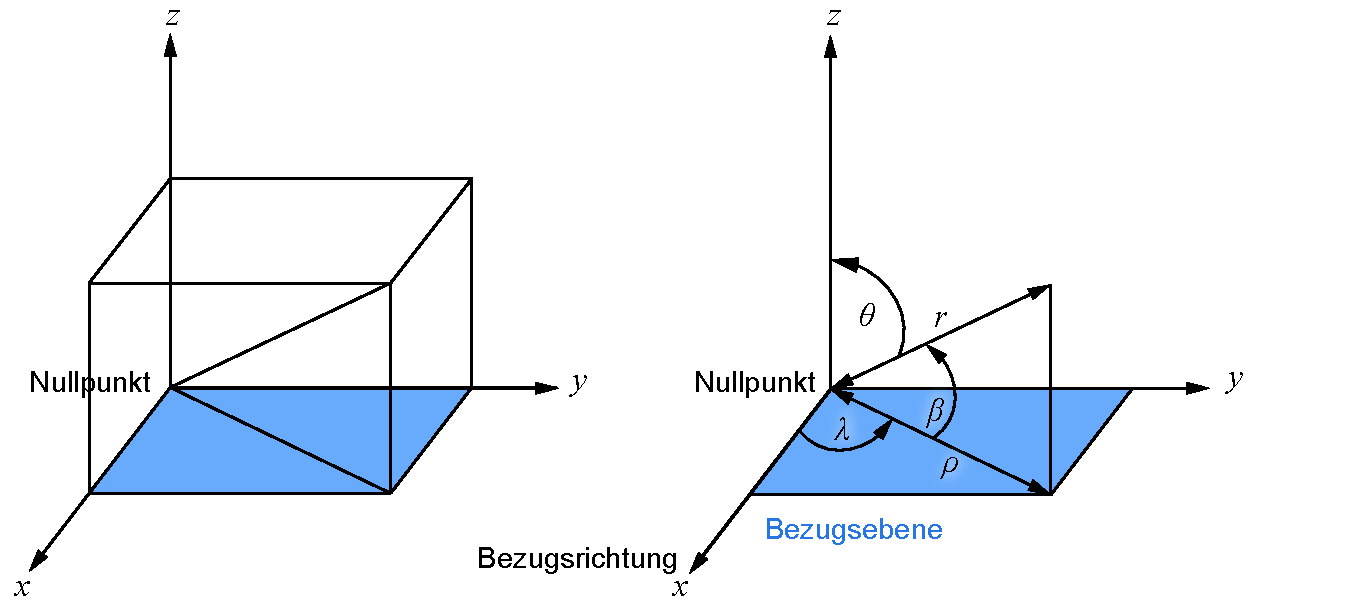
\includegraphics[width=\textwidth]{Koordinatensysteme.pdf}%
\caption[Koordinatensysteme in kartesischen und sph�rischen Polarkoordinaten.]{Koordinatensysteme in kartesischen und (astronomischen) sph�rischen Polarkoordinaten. Gegen�ber dem mathematischen sph�rischen KOS nutzt man im astronomischen sph�rischen KOS den Winkel $\beta = 90\degree -\theta$.}%
\label{abb:hm_koordinatensysteme}%
\end{figure}
Die Umrechnung zwischen den beiden Koordinatensystemen ist gegeben durch
\begin{align*}
x &= r\,\cos\beta\,\cos\lambda ~,\\
y &= r\,\cos\beta\,\sin\lambda ~,\\ 
z &= r\,\sin\beta ~.\\ 
\smallskip
r &= \sqrt{\rho^2 + z^2} &&\text{ mit } \rho=\sqrt{x^2+y^2} \,,  \nonumber\\
\beta &= \arctan(z/\rho) &&\text{ f�r } \rho\neq 0 \text{; ansonsten 0\textdegree, 90\textdegree\ oder -90\textdegree\ je nach Quadrant.} \nonumber\\
\psi &= 2\arctan\lk \frac{y}{\abs{x}+\rho} \rk\,, \nonumber\\
\lambda &= \psi &&\text{f�r } x=0 \text{ und } y>0 \text{ (auf der positiven $y$-Achse)} \,,\nonumber\\
\lambda &= \psi &&\text{f�r } x>0 \text{ und } y\geq 0 \text{ (1. Quadrant)} \,, \nonumber\\
\lambda &= 360\text{\textdegree}+\psi &&\text{f�r } x\geq 0 \text{ und } y<0 \text{ (4. Quadrant)} \,,\nonumber\\
\lambda &= 180\text{\textdegree}-\psi &&\text{f�r } x<0 \text{ (2. und 3. Quadrant)} \,,\nonumber\\
\lambda &= 0\text{\textdegree} &&\text{f�r } x=0 \text{ und } y=0 \text{ (im Ursprung)} ~~. \nonumber
\end{align*}
Bei der Berechnung der arctan-Funktionen muss man etwas aufpassen und sich �berlegen, in welchem Quadranten der Winkel liegt.
In \matlab{} ist dazu die Funktion atan2 hinterlegt, die \iw der hier angegebenen Berechnung f�r $\psi$ entspricht und vor allem bei ganzzahligen Vielfachen von $\pi$ f�r $\psi$ genauere Werte liefert.
Die Formel l�sst sich leicht �ber die Beziehung f�r den Tangens des halben Winkels herleiten. Dazu formt man diese �ber
	\[
	\tan\lk \frac{\psi}{2} \rk= \frac{-x \pm \sqrt{x^2+y^2}}{y} = \cot \lk\frac{\psi}{2}-90\degree \rk
\]
um und stellt dann die entsprechenden Fallunterscheidungen f�r $x$ und $y$ an.

F�r die Himmelsmechanik empfehlen sich nun zur Festlegung eines KOS zwei nat�rlich \anf{ausgezeichnete} Bezugsebenen:
\begin{itemize}
\item Die Bahnebene\index{Bahnebene}\footnote{Wir haben ja bereits im Kapitel 1 von Band I gezeigt, dass die Bewegung eines K�rpers im Zentralkraftfeld wegen der Drehimpulserhaltung in einer Ebene stattfindet.  
Wir k�nnen deshalb die Bewegung in einer Bahnebene als gesichert annehmen. In \kapitel{hm_bewegungsgl} werden wir das noch einmal detailliert zeigen.} der Erde um die Sonne (\emph{\gls{ekliptik}}).
\item Die Ebene, die durch den Erdmittelpunkt geht und senkrecht zur Erdachse liegt (\emph{�quatorebene} \index{Aequator@�quator}).
\end{itemize}
Die Schnittlinie zwischen der Ekliptik und der �quatorebene ergibt dann eine besonders ausgezeichnete gemeinsame Bezugsrichtung/Bezugslinie.
Schaut man auf dieser Bezugslinie (\figref{hm_ekliptik-aequator}) von der Erde in Richtung zur Sonne, dann wird der Schnittpunkt der Erdbahn, wenn diese die Bezugslinie in der Richtung vom Himmelss�dpol zum Himmelsnordpol\footnote{Als Himmelspole\index{Himmelspol} werden die Durchsto�punkte der Erdachse mit der gedachten Himmelskugel bezeichnet.} schneidet, \emph{\gls{fruehlingspunkt}} $\vernal$ genannt.\footnote{Im geozentrischen Bild, das wir gleich noch erl�utern werden, kann man den Fr�hlingspunkt\index{Fr�hlingspunkt|textbf} auch als Schnittpunkt der Sonnenbahn mit dem Himmels�quator auf der gedachten Himmelskugel betrachten (wiederum in der Richtung von S�d nach Nord).} 
Die beiden Ebenen (Ekliptik, �quator) und die Richtung von Erde zum Fr�hlingspunkt dienen somit als Grundlage f�r verschiedene astronomische Koordinatensysteme.
Als Nullpunkt kann der Beobachtungsort entweder im Sonnen- (heliozentrisch\index{Koordinatensystem!heliozentrisches}) oder Erdmittelpunkt (geozentrisch\glslink{geozentrkoord}) gew�hlt werden -- beides keine besonders komfortablen, daf�r aber mathematisch sehr vorteilhafte Beobachtungspunkte.\footnote{An dieser Stelle sei noch einmal auf die grunds�tzliche Raum-Zeit-Problematik in der Himmelsmechanik hingewiesen: Weder der �quator (\bzw die Polachse der Erde) noch die Ekliptik sind wirklich fest im Raum, sondern sie werden durch Kr�fte der verschiedenen Himmelsk�rper in ihrer Lage ver�ndert. Deshalb muss zu jeder Angabe von Koordinaten in einem bestimmten Koordinatensystem eine Zeitangabe gemacht werden.} 
\begin{figure}%
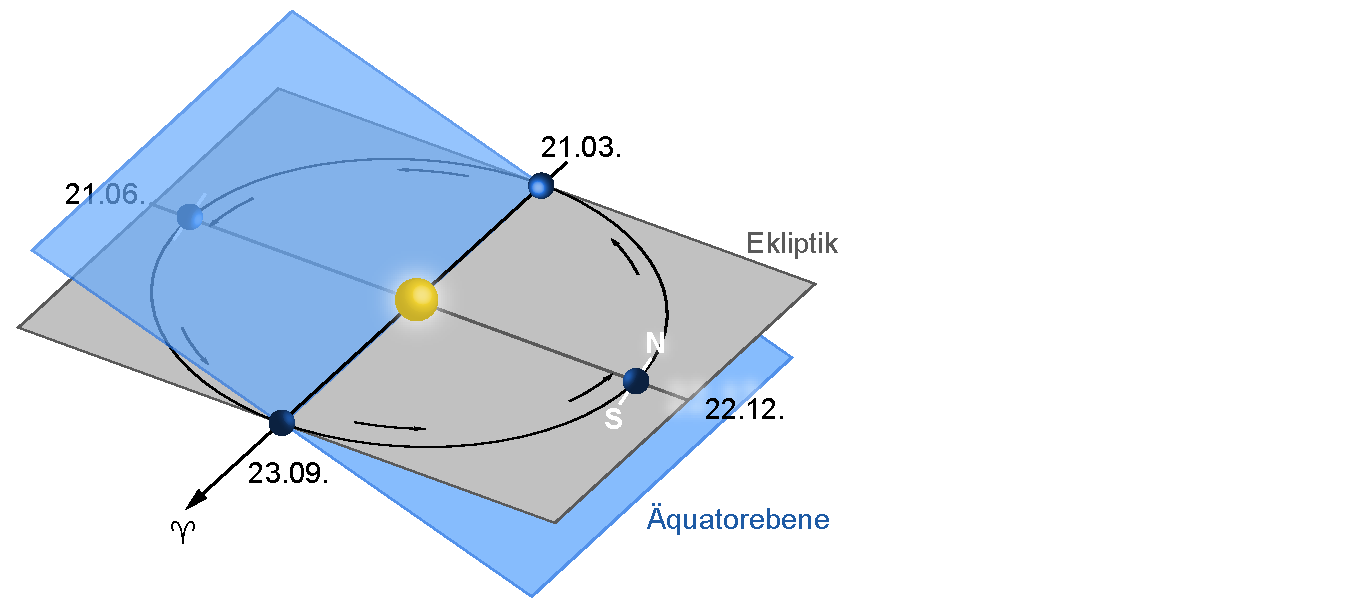
\includegraphics[width=\textwidth]{EkliptikAequator.pdf}%
\caption{Ekliptik, �quator und Fr�hlingspunkt.}%
\label{abb:hm_ekliptik-aequator}%
\end{figure}

Weitere ausgezeichnete Bezugsebenen sind die Bahnebene eines Himmelsk�rpers und die Horizontebene\index{Horizontebene} eines Beobachters auf der Erdoberfl�che: Beide sind f�r Beobachtungsdaten sehr wichtig.
Die Wahl von Bezugsebene, Bezugsrichtung ($x$-Achse) und Nullpunkt (Ursprung) ergeben die verschiedenen Koordinatensysteme, die wir in Tabelle \ref{tab:hm_astro_KOS} zusammengefasst haben.
F�r eine tiefergehende Darstellung der verschiedenen Koordinatensysteme empfehlen wir die Darstellungen in \cite{Montenbruck1999,Praxl2016,Meeus1998}. \\
Wir geben in \figref{hm_geozent_KOS} die graphische Darstellung des geozentrisch-ekliptikalen KOS\index{Koordinatensystem!geozentrisch-ekliptikales} (GE) und des geozentrisch-�quatorialen KOS\index{Koordinatensystem!geozentrisch-�quatoriales} (GA) an.
Letzteres rotiert mit dem Fixsternhimmel mit, ist also fest mit diesem verbunden und wird deswegen auch \emph{space-fixed} GA-KOS genannt (GA(sf)).
Die Definition der zum jeweiligen System geh�renden Koordinaten ist in \figref{hm_geozent_KOS} ersichtlich und im Detail in Tabelle \ref{tab:hm_astro_KOS} aufgef�hrt.

\begin{figure}%
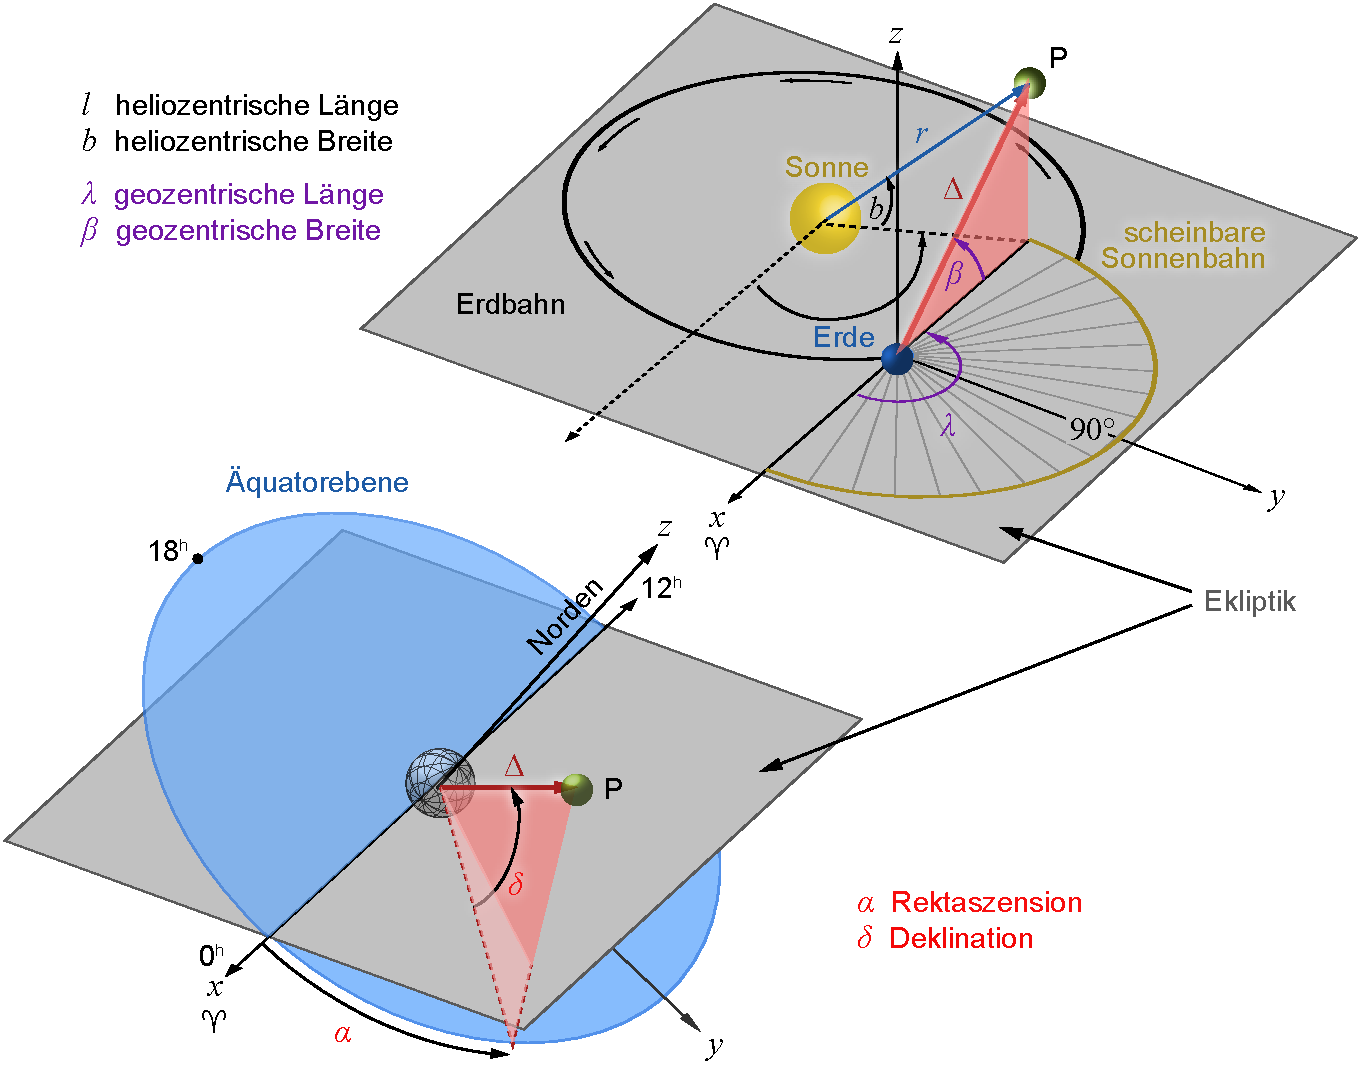
\includegraphics[width=\textwidth]{GE_und_GAe_KOS.pdf}%
\caption[Geozentrisch-ekliptikales und geozentrisch-�quatoriales KOS]{Geozentrisch-ekliptikales und geozentrisch-�quatoriales KOS. Die einzelnen Parameter und ihre Beziehungen zueinander sind im Detail in Tabelle \ref{tab:hm_astro_KOS} erl�utert.}%
\label{abb:hm_geozent_KOS}%
\end{figure}

Die Umrechnungen zwischen den einzelnen KOS haben wir in Tabelle \ref{tab:hm_Umrechung_KOS} im Tabellenanhang angegeben.
Die Herleitung kann �ber die Formeln der sph�rischen Trigonometrie \cite{Smart1986} oder eleganter �ber Rotations- bzw. Drehmatrizen\index{Rotationsmatrix} \index{Drehmatrix} (siehe Kap. 1.2 in Band I \bzw \cite{Montenbruck1999}) erfolgen, da die Transformationen zwischen den einzelnen Koordinatensystemen jeweils durch Drehungen und/oder Translationen beschrieben werden k�nnen.
Wir wollen das am Beispiel der Transformation des Ortsvektors $\vec{r}$ im geozentrisch-ekliptikalen KOS (GE) in den Ortsvektor $\vec{r}'$ des geozentrisch-�quatorialen KOS (GA(sf)) demonstrieren.
Diese Transformation entspricht, wie wir aus \figref{hm_geozent_KOS} erkennen, einer Drehung um die $x$-Achse um die \emph{Schiefe der Ekliptik}\index{Schiefe der Ekliptik} $\epsilon$.
Der Winkel $\epsilon$ ist identisch zur Neigung der Erdachse\index{Neigung Erdachse} gegen ihre Bahnebene.
Die entsprechende Drehung wird durch folgende Matrizen beschrieben:
\begin{align}
\begin{split}
\vec{r}' &= \mathbb{R}_x(-\epsilon)\cdot \vec{r} = \lk \begin{array}{ccc} 1 & 0 & 0 \\ 0 & \cos\epsilon & -\sin\epsilon \\ 0 & \sin\epsilon & \cos\epsilon \end{array}\rk \lk \begin{array}{c} x \\ y\\ z \end{array}\rk ~,~~~\vec{r}' = \lk \begin{array}{c} r\cos\delta\cos\alpha \\ r\cos\delta\sin\alpha \\ r\sin\delta \end{array}\rk\,,\\
\vec{r} &= \mathbb{R}_x(\epsilon)\cdot \vec{r}' = \lk \begin{array}{ccc} 1 & 0 & 0 \\ 0 & \cos\epsilon & \sin\epsilon \\ 0 & -\sin\epsilon & \cos\epsilon \end{array}\rk \lk \begin{array}{c} x' \\ y' \\ z' \end{array}\rk \,, ~~~ \vec{r} = \lk \begin{array}{c} r\cos\beta\cos\lambda \\ r\cos\beta\sin\lambda \\ r\sin\beta \end{array}\rk \,.
\end{split} \label{eq:hm_drehung_x_achse1}
\end{align}

\begin{sidewaystable}
\vspace{12cm}
\caption{Astronomische Koordinatensysteme und deren Parameter.}
\begin{tabular}{L{1cm}|L{3.5cm}|L{2cm}|L{2cm}|L{2cm}|L{2cm}|L{3cm}l}
\hline\noalign{\smallskip}
Kurz-		& Bezeichnung &	Ursprung  & Bezugs- & Bezugsrichtung  &	Vertikale  & Horizontale &	Koordinaten \\
zeichen &							&						& ebene		& $x$-Achse				& Koordinaten	& Koordinaten &							\\
\noalign{\smallskip}\svhline\noalign{\smallskip}
\multicolumn{8}{l}{Absolute Systeme}	\\					
\noalign{\smallskip}\svhline\noalign{\smallskip}	
BA & Bahnkoordinaten & Zentralk�rper & Bahn & \gls{periapsis} & - &	Abstand $r$, \linebreak Anomalie $\upsilon$  & $\lk \begin{array}{c} r\,\cos \upsilon \\r\,\sin \upsilon \\ 0 \end{array}\rk$ \\
BA & Bahnkoordinaten & Zentralk�rper & Bahn & Knoten\index{Knoten} & - &	Abstand $r$,\linebreak Winkel $u\!=\!\upsilon\!+\!\omega$,\linebreak L�nge der Periapsis $\omega$ & $\lk \begin{array}{c} r\,\cos u \\r\,\sin u \\ 0 \end{array}\rk$\\
HE & Heliozentrisch-ekliptikal & Sonne (Mittelpunkt) & Ekliptik & $\vernal$ & Ekliptikale Breite $b$ & Ekliptikale L�nge $l$ & $\lk \begin{array}{c} r\,\cos b\,\cos l \\ r\,\cos b\,\sin l \\ r\,\sin b \end{array}\rk$\\
GE & Geozentrisch-ekliptikal & Erde (Mittelpunkt) & Ekliptik & $\vernal$ & Ekliptikale Breite $\beta$ & Ekliptikale L�nge $\lambda$	& $\lk \begin{array}{c} \Delta\,\cos \beta\,\cos \lambda \\ \Delta\,\cos \beta \,\sin \lambda \\ \Delta\,\sin \beta \end{array}\rk$\\
GA(sf) & Geozentrisch-�quatorial (space-fixed) & Erde (Mittelpunkt) & �quator & $\vernal$ & \gls{dekl} $\delta$ & \gls{rektasz} $\alpha$ & $\lk \begin{array}{c} \Delta\,\cos \delta\,\cos \alpha \\ \Delta\,\cos \delta\,\sin \alpha \\ \Delta\,\sin \delta \end{array}\rk$\\
\noalign{\smallskip}\svhline\noalign{\smallskip}
\multicolumn{8}{l}{Relative Systeme}	\\					
\noalign{\smallskip}\svhline\noalign{\smallskip}	
GA(ef) & Geozentrisch-�quatorial (earth-fixed) & Erde (Mittelpunkt) & �quator & Meridian (Greenwich) & Deklination $\delta$ & Stundenwinkel $\tau$ & $\lk \begin{array}{c} \Delta\,\cos \delta\,\cos \tau \\ \Delta\,\cos \delta\,\sin \tau \\ \Delta\,\sin \delta \end{array}\rk$\\
TA & Topozentrisch-�quatorial & Topozentrum (Beobachter) & Parallele \linebreak (zum �quator) & Meridian (Greenwich) & Deklination $\delta'$ & Stundenwinkel $\tau$ & $\lk \begin{array}{c} \Delta'\,\cos \delta' \,\cos \tau \\ \Delta'\,\cos \delta'\,\sin \tau \\ \Delta'\,\sin \delta' \end{array}\rk$\\
TH & Topozentrisch-horizontal & Topozentrum (Beobachter) & Horizont & S�den (Meridian) \linebreak Beobachter & H�henwinkel $h$ & Azimut $\mathcal{A}$ & - \\
\noalign{\smallskip}\hline\noalign{\smallskip}
\end{tabular}
\label{tab:hm_astro_KOS}
\end{sidewaystable}


Daraus ergeben sich dann folgende Umrechnungsformeln f�r GE nach GA(sf):
\begin{align}
\cos\delta\cos\alpha &= \cos\beta\cos\lambda  \,, \label{eq:hm_drehung_x_achse_linear2} \\
\cos\delta\sin\alpha &= \cos\beta\sin\lambda\cos\epsilon - \sin\beta\sin\epsilon \nonumber \,,\\
\sin\delta &= \cos\beta\sin\lambda\sin\epsilon + \sin\beta\cos\epsilon  \nonumber ~~.
\end{align}
In umgekehrter Richtung von GA(sf) nach GE gilt dann:
\begin{align}
\cos\beta\cos\lambda &= \cos\delta\cos\alpha \,,\label{eq:hm_drehung_x_achse_linear_3} \\ 
\cos\beta\sin\lambda &= \cos\delta\sin\alpha\cos\epsilon + \sin\delta\sin\epsilon \nonumber \,,\\
\sin\beta &= \sin\delta\cos\epsilon - \cos\delta\sin\alpha\sin\epsilon  \nonumber ~~.
\end{align}
In \probref{hm_trafo_koord} werden die Dreh- und Translationsmatrizen f�r die in Tabelle \ref{tab:hm_Umrechung_KOS} im Tabellenanhang aufgef�hrten KOS-Transformationen verifiziert. \\
Im Gegensatz zu den beiden gerade besprochenen absoluten Koordinatensystemen\index{Koordinatensystemen!absolutes} sind das geozentrisch-�quatoriale (\emph{earth-fixed}) KOS (GA(ef)) ebenso wie das topozentrisch-horizontale KOS\index{Koordinatensystem!horizontales} (TH) wegen der Erdrotation von der Zeit abh�ngig und geh�ren damit zur Gruppe der relativen KOS.
F�r die Umrechnung zwischen dem raum-fixierten geozentrisch-�quatorialen System\index{Koordinatensystem!geozentrisch-�quatoriales} (GA(sf)) und dem erd-fixierten geozentrisch-�quatorialen System (GA(ef)) f�hrt man den \gls{stundenwinkel} $\tau$ ein.
\gls{rektasz} $\alpha$ und Stundenwinkel $\tau$ sind die einander entsprechenden Koordinaten im GA(sf) bzw. GA(ef)-Koordinatensystem.
Die Rektaszension\index{Rektaszension} ist definiert als Winkel entlang des �quators zwischen der Richtung zum Fr�hlingspunkt\index{Fr�hlingspunkt} $\vernal$ (Bezugsrichtung der Rektaszension) und der Richtung zum Himmelsobjekt (\figref{hm_geozent_KOS} und Tabelle \ref{tab:hm_astro_KOS}).
Die Bezugsrichtung f�r den Stundenwinkel\index{Stundenwinkel} hingegen ist der ortsfeste \gls{meridian} (die S�drichtung).
Der Stundenwinkel eines betrachteten Himmelsk�rpers gibt damit die Differenz zwischen der Rektaszension $\alpha$ dieses K�rpers und der Rektaszension derjenigen Himmelsk�rper an, die gerade ihre gr��te H�he �ber dem Horizont im Meridian erreichen.
Der Stundenwinkel gibt also die Zeit an, die ein Himmelsk�rper noch bis zu seiner \gls{kulmination} braucht bzw. die seit seiner \gls{kulmination} schon verstrichen ist.\footnote{Der Stundenwinkel ist ein Winkel- und Zeitma�. Wir werden in \kapitel{hm_zeitdefinition} den wichtigen Zusammenhang zwischen dem Stundenwinkel und der dort definierten Sternzeit ableiten.} 

\begin{figure}%
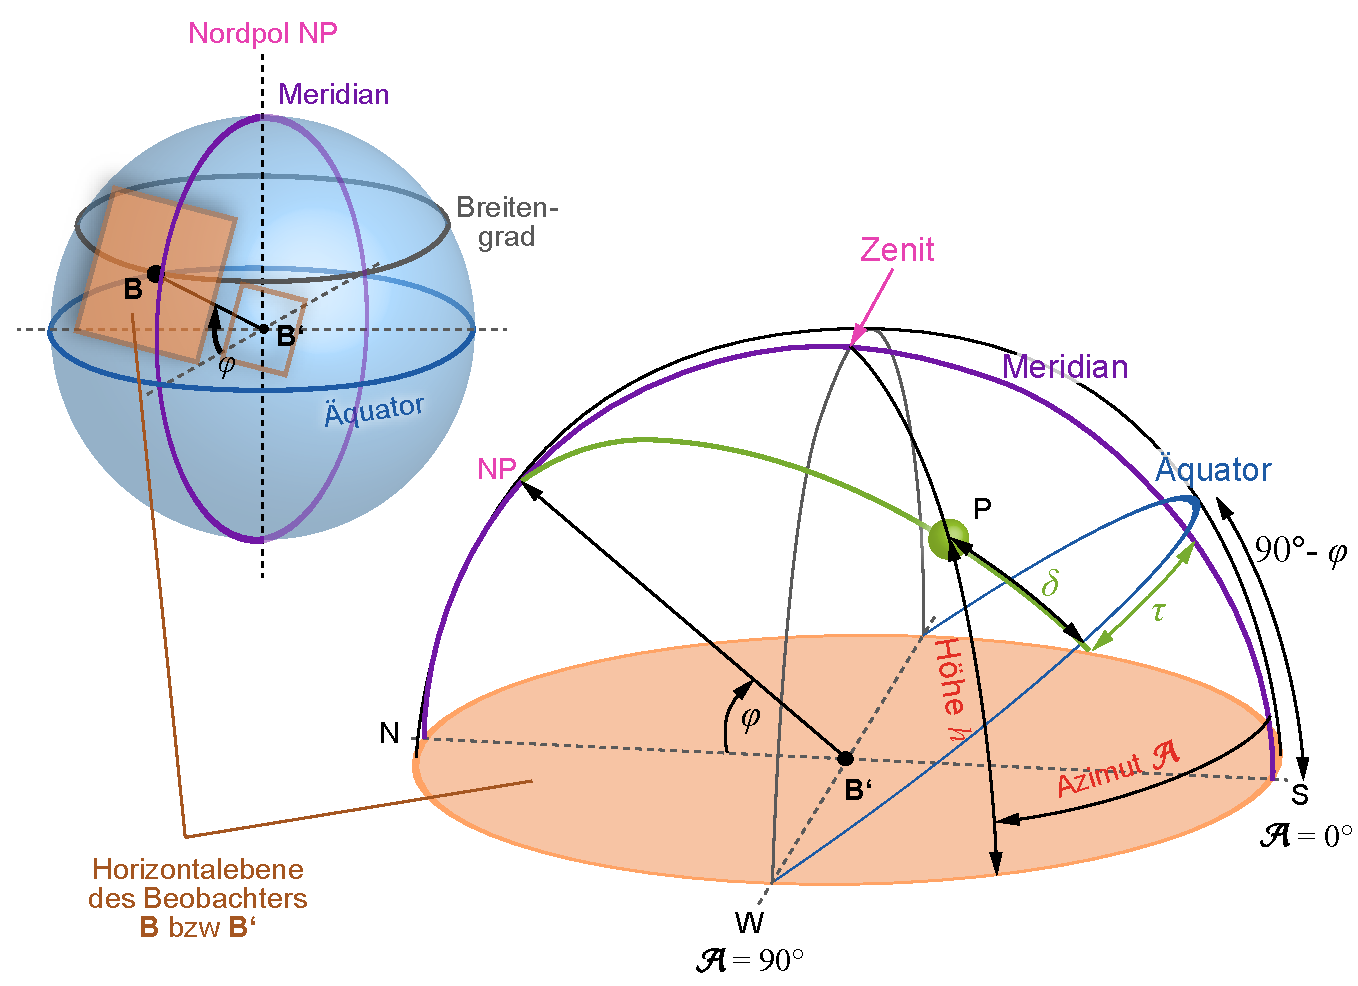
\includegraphics[width=\textwidth]{TH01.pdf}%
\caption{Topozentrisches Horizontalkoordinatensystem.}%
\label{abb:hm_topozent_KOS}%
\end{figure}

Wir betrachten nun noch das topozentrisch-horizontale KOS\index{Koordinatensystem!topozentrisches} (TH) (\figref{hm_topozent_KOS}) etwas genauer.
Dieses stellt f�r den Beobachter auf der Erde das nat�rlichste KOS dar und ist \zb f�r die Berechnung von Aufgangs- und Kulminationszeiten das geeignete Bezugssystem.
Das topozentrisch-horizontale KOS geht offensichtlich durch Drehung um die $y$-Achse um den Winkel $90$\textdegree$-\varphi$ aus dem �quatorialen KOS hervor.\footnote{Die von der Erdoberfl�che aus gemessenen Horizontal- und Vertikalkoordinaten $\alpha',\delta'$ im TA-KOS weichen im Allgemeinen wenig von den gemessenen im GA-KOS $\alpha,\,\delta$ ab.
Ausnahmen sind die Beobachtungen von erdnahen Objekten wie \zb Satelliten, Monden, Kometen und benachbarten Planeten.} Der Beobachter B im topozentrisch-horizontalen KOS befindet sich an einem Ort der \emph{\glslink{geogrkoord}{geographischen Breite}} $\varphi$.
F�r ihn ist dann der jeweilige Himmelspol unter dem Winkel $\varphi$ zu sehen.
Der rechte Teil der \figref{hm_topozent_KOS} zeigt dies f�r die Nordhalbkugel.
Als Meridian\index{Meridian} wird der Gro�kreis an der Himmelskugel bezeichnet, auf dem S�dpunkt und Nordpunkt am Horizont, der \gls{zenit} und die beiden Himmelspole liegen.
Eine h�ufig benutzte Beziehung zwischen dem �quatorialen KOS und dem topozentrisch-horizontalen KOS ist die Berechnung von H�he und \gls{azimut} eines Himmelsk�rpers aus bekannter Deklination und bekanntem Stundenwinkel.
Diese Beziehung l�sst sich wiederum mit Hilfe der Matrizentransformation f�r die Umrechnung der KOS ableiten (Tabelle \ref{tab:hm_Umrechung_KOS}, \probref{hm_trafo_koord}):
\begin{merksatz}{Umrechnung vom �quatorialen KOS in das topozentrisch-horizontale KOS}
\begin{align}
\begin{split}
\sin h &= \cos\delta\cos\tau\cos\varphi+\sin\delta\sin\varphi \,,\\
\tan \mathcal{A} &= \frac{\cos\delta\sin\tau}{\cos\delta\cos\tau\sin\varphi-\sin\delta\cos\varphi} \,. 
\end{split} \label{eq:hm_Alt-Az-Koord}
\end{align}

\end{merksatz}
Wir haben bereits darauf hingewiesen, dass die Bezugsebenen und Bezugsrichtungen der genannten KOS nicht fest im Raum liegen.
Vielmehr f�hren diese durch Kr�fte von anderen Himmelsk�rpern als (astronomische) Pr�zession\index{Pr�zession} bekannte Kreiselbewegungen aus, die wir bereits in Kapitel 1.5.5 im Band I mit einer Modellrechnung untersucht hatten und die in den Referenzen \cite{Montenbruck1999, Murray2008} detailliert beschrieben wird.
So verschiebt sich der Fr�hlingspunkt pro Jahr um etwa 50 Bogensekunden in westlicher Richtung entlang der Ekliptik.
Dieser Effekt ist so gro�, dass er bereits �ber relativ kurze Beobachtungszeitr�ume von einigen Jahren auff�llt.
Damit verschieben sich auch die Nullpunkte der astronomischen Koordinatensysteme langsam entlang der Ekliptik und die ekliptikale L�nge eines Sterns ohne Eigenbewegung nimmt in einem Jahr um \ca 50 Bogensekunden zu.
Die Koordinaten eines Himmelsobjekts �ndern sich also, ohne dass dies einer eigentlichen Bewegung des Objekts entspricht.\footnote{Der Pr�zessionsbewegung �berlagern sich noch zus�tzliche periodische Schwankungen. Diese verschiedenen periodischen Bewegungen, welche die Erdachse zus�tzlich zur Pr�zession ausf�hrt, werden in der Astronomie unter dem Begriff der Nutation\index{Nutation} zusammengefasst. Die Ursachen sind nicht vollst�ndig identisch mit der im Kapitel 1, Band I hergeleiteten Nutation eines schweren Kreisels, aber die Bewegungsform ist sehr �hnlich. Die Verschiebung der �quinoktialpunkte\index{Aequinoktialpunkte@�quinoktialpunkte} entlang der Ekliptik erfolgt also nicht v�llig gleichm��ig, sondern mit periodisch leicht schwankender Geschwindigkeit.}
Deshalb braucht es zur Angabe von Koordinaten von Himmelsk�rpern auch stets den Zeitpunkt, auf den sich die Koordinaten beziehen.
Von besonderer Bedeutung f�r Beobachtungen sind die Koordinaten f�r das �quinoktium des Beobachtungszeitpunkts, das sogenannte \emph{�quinoktium des Datums}\glslink{aequinox}.
Der Begriff \emph{�quinoktium} \index{Aequinoktium@�quinoktium} bezeichnet hier den tats�chlichen, aktuellen Schnittpunkt des Himmels�quators mit der Ekliptik zum Beobachtungszeitpunkt.
Mit \emph{\gls{epoche}}\index{Epoche} wird in der Himmelsmechanik der Zeitpunkt einer Beobachtung bezeichnet.\footnote{Merkregel: Die Epoche bezeichnet den tats�chlichen Zeitpunkt einer Beobachtung oder eines Vorgangs, das �quinoktium das Koordinatensystem, in dem gemessen wird.} Vielfach werden Koordinaten auf Koordinatensysteme sogenannter Stan\-dard\-�qui\-noktien\index{Standard�quinoktium} bezogen, die sich auf bestimmte feste Zeitpunkte (etwas verwirrend auch \emph{Standardepochen}\index{Standardepoche} genannt) beziehen.
\emph{�quinoktium und Epoche J2000} bedeuten \zb dass sich die Koordinatensysteme, Bahnparameter und die Ekliptikschiefe\index{Ekliptikschiefe} $\epsilon$ auf die Lage von �quator, Ekliptik und Fr�hlingspunkt zum 01.\,01.\,2000 beziehen und dass am 01.\,01.\,2000 beobachtet wurde.
F�r diese Epoche gilt beispielsweise $\epsilon\!=\!23.4392911$\text{\textdegree}.
Wir werden im Folgenden f�r die Berechnung von Beobachtungsdaten von Himmelsk�rpern, falls nicht anders angegeben, das �quinoktium dieses Datums benutzen. 

\begin{figure}%
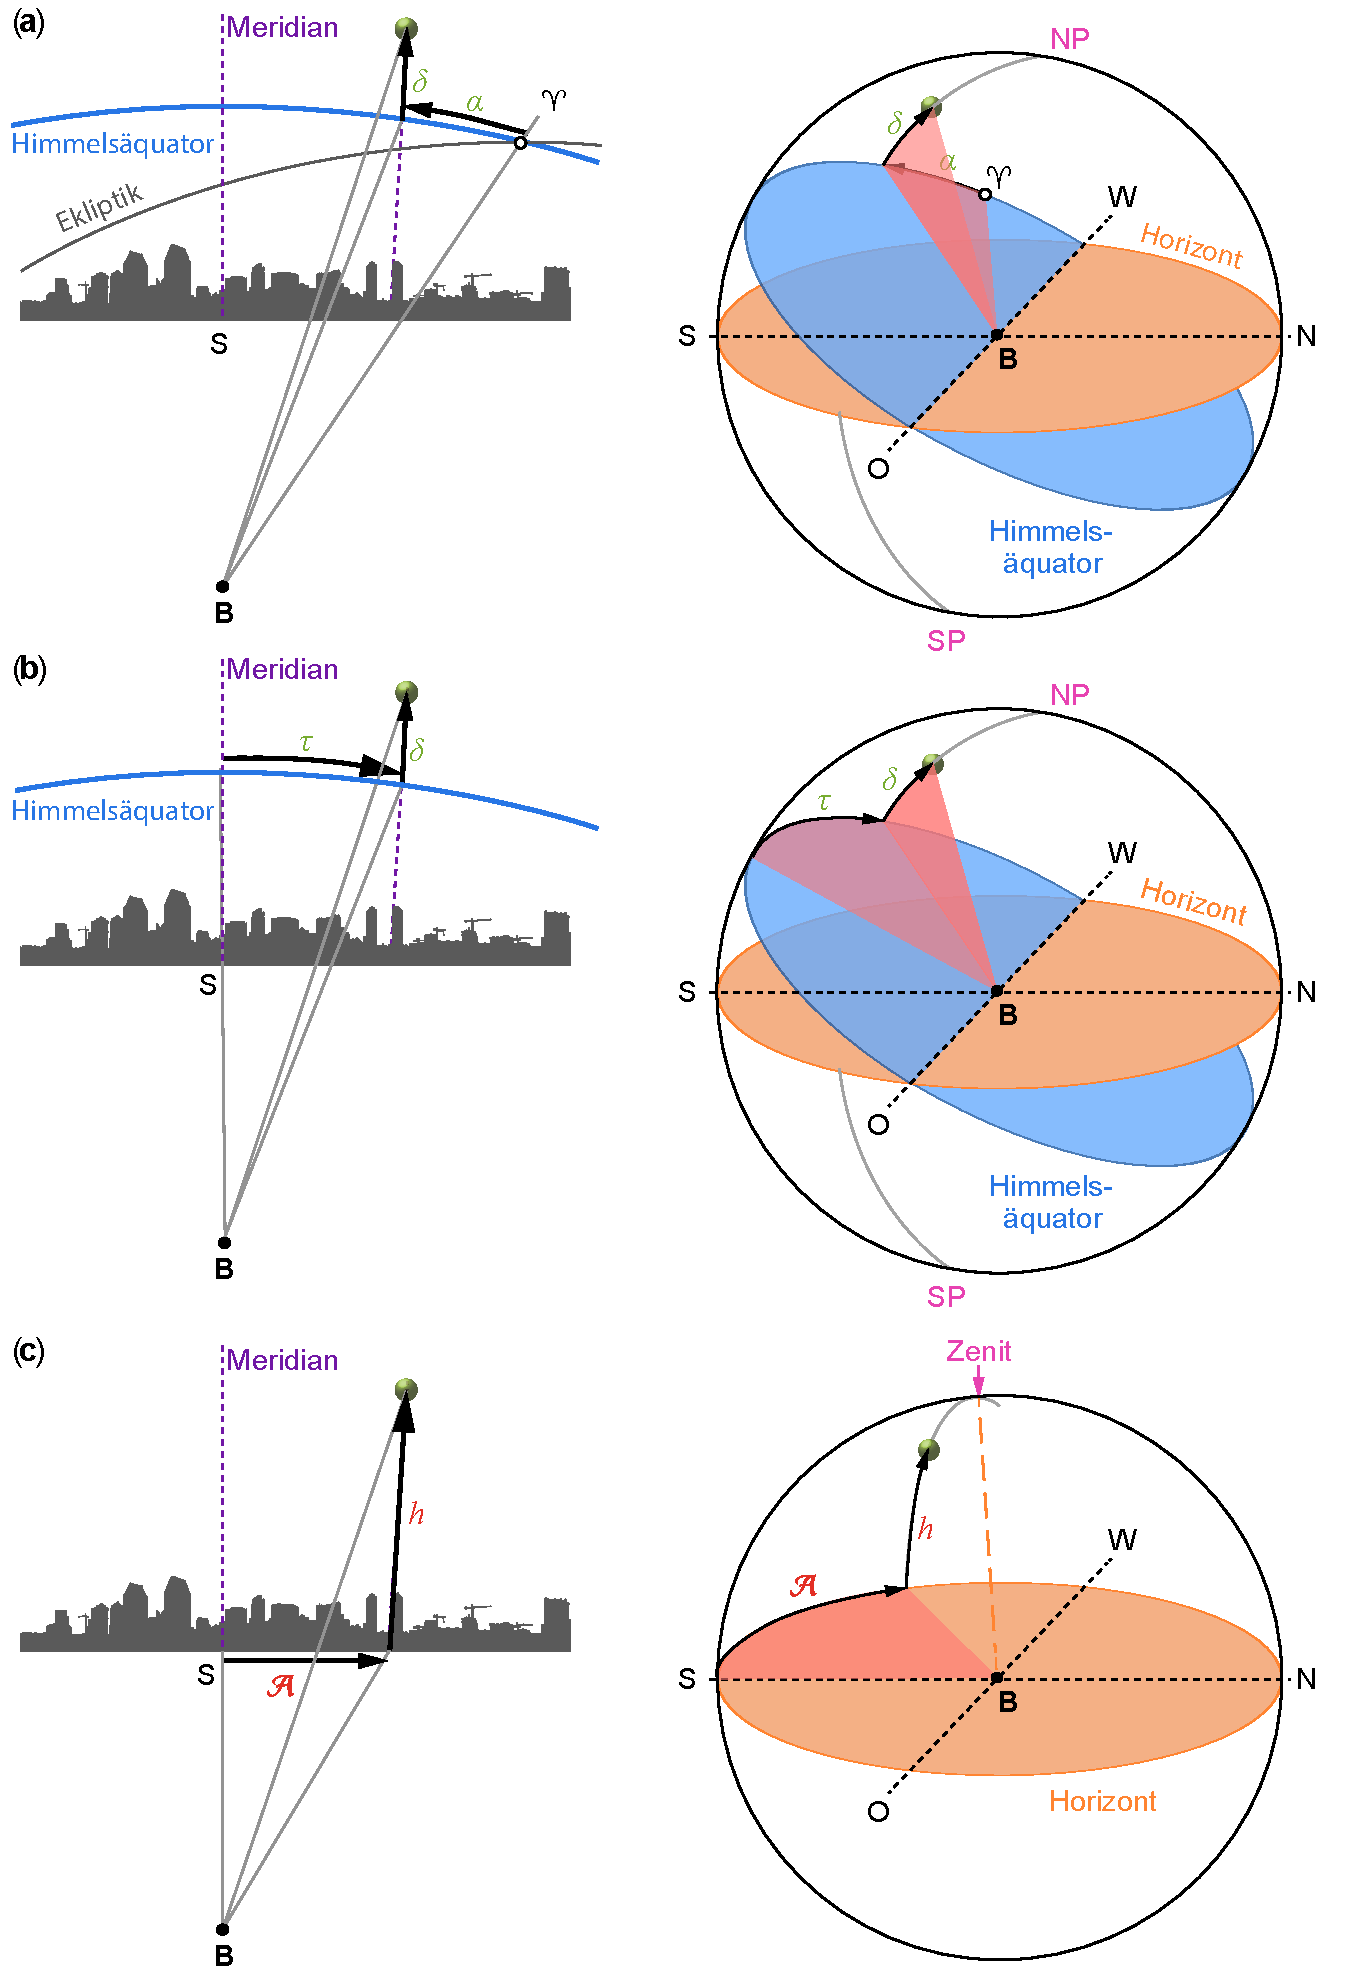
\includegraphics[width=\textwidth]{KOS_Vgl.pdf}%
\caption[Zusammenh�nge zwischen h�ufig benutzten Koordinatensystemen.]{Zusammenh�nge zwischen h�ufig benutzten Koordinatensystemen. \fa Raum-fixiertes geozentrisch"=�quatoriales KOS (GA(sf)), \fb Erd-fixiertes geozentrisch-�quatorales KOS (GA(ef)), \fc Topozentrisch-horizontales KOS (TH).}%
\label{abb:hm_KOS_Abh}%
\end{figure}
\figref{hm_KOS_Abh} fasst noch einmal schematisch die Zusammenh�nge zwischen den verschiedenen gebr�uchlichen KOS zusammen.
Wir wollen uns nun im n�chsten Kapitel etwas n�her mit dem Aspekt der Zeit besch�ftigen.

\subsection{Zeitdefinition}\label{kap:hm_zeitdefinition}
Zeit beschreibt die Abfolge von Ereignissen, hat also eine eindeutige, unumkehrbare Richtung.
Sie wird in ihrer Skala durch wiederkehrende, periodische Vorg�nge definiert, wie sie auch in der Himmelsbeobachtung gegeben sind.
Wir stellen zun�chst die in der Astronomie �bliche \glslink{jd}{Julianische Tagesz�hlung}\index{Julianisches Datum} (\emph{Julian Date}\footnote{Das Julianische Datum wurde 1582 vom Franzosen Joseph Justus Scaliger (1540--1609) eingef�hrt. Nach einer nicht gesicherten Darstellung w�hlte er die Bezeichnung, um damit seinen Vater Julius Scaliger zu ehren und nicht, wie h�ufig vermutet, Julius Caesar.} JD) vor, bei der die Tage fortlaufend seit dem 01.\,01.\,($-$4712) (entspricht dem 01.\,01.\,4713 v. Chr.) durchgez�hlt werden.
Ein neuer Tag im JD beginnt jeweils um 12:00 am Mittag.\footnote{Dank dieser Konvention braucht bei astronomischen Beobachtungen w�hrend der Nacht kein \anf{Datumswechsel} vollzogen zu werden.} So entspricht dem 01.\,01.\,2020 0:00 UT (Mitternacht in Greenwich\footnote{Wir verwenden hier schon die sogenannte Universal Time UT, die wir erst sp�ter genauer definieren. Vorerst gen�gt die Annahme, dass wir eine Uhr haben, die wir UT nennen, auf der unsere astronomische Zeitz�hlung beruht.}) das Julianische Datum J\,2458849.5,
dem 01.\,01.\,2021 das Julianische Datum\index{Julianische Datum} J\,2459215.5, dazwischen liegen demzufolge $\text{J\,}2458849.5 - \text{J\,}2459215.5\!=\!366\,\text{Tage}$, denn 2020 war ein Schaltjahr.
H�ufig wird auch das \emph{Modifizierte Julianische Datum} MJD\index{Datum!Modifiziertes Julianisches} verwendet, welches als $\text{MJD}\!=\!\text{JD\,}-2400000.5$ definiert wird.
Ferner sei noch angemerkt, dass ein nach dem JD berechnetes Julianisches Jahrhundert immer ganzzahlige $36525$ Tage hat, die man in exakt $24$ Stunden zu $3600$ Sekunden unterteilt.
Es gibt in Computerprogrammen (so auch in \matlab) hinterlegte Routinen zur Berechnung des JD aus dem Kalenderdatum und umgekehrt \cite{Praxl2016,Meeus1998}.
Mit dem Julianischen Datum haben wir eine elegante Z�hlung beschrieben, mit der wir in der Himmelsmechanik sowohl gro�e als auch kleine Zeitr�ume, wie \zb Tagesabschnitte, einheitlich beschreiben k�nnen. 
Wir m�ssen aber neben der durch das JD definierten Z�hlweise auch die zugrundeliegende Zeit physikalisch definieren.
Es sind verschiedene Zeitdefinitionen m�glich, und wir unterscheiden (siehe auch \cite{McCarthy2018}):
\begin{itemize}
    \item durch Bewegungsgesetze definierte \emph{dynamische} Zeitskalen (\zb Ephemeridenzeit\footnote{Als \emph{\gls{ephemeride}}\index{Ephemeride} wird ganz allgemein die Positionsangabe eines Himmelsk�rpers bezogen auf ein bestimmtes KOS bezeichnet. Himmelsmechanik ist also nichts anderes als die Bestimmung der Ephemeriden als Funktion der Zeit.} ET),
    \item Realisierungen durch eine absolut \emph{gleichm��ig ablaufende} Zeit (Atomzeit TAI),
    \item die b�rgerliche oder \emph{Alltagszeit} (Universal Time UT, Universal Time Coordinated UTC) und
    \item \emph{erdrotationsabh�ngige} Zeitskalen (Wahre Sonnenzeit und Sternzeit).
\end{itemize}

\subparagraph{Dynamische Zeit:}
F�r die Berechnungen in der Himmelsmechanik ben�tigen wir die dynamische Zeit.
Das ist die Zeit, die auch in den zeitlichen Ableitungen der Bewegungsgleichungen \anf{steckt}.
Sinnvollerweise benutzt man zur Zeitma�definition periodische Bewegungen der Himmelsk�rper.
Die Umlaufdauer\index{Umlaufzeit} der Erde um die Sonne ist weitgehend konstant, und man definiert daher den zeitlichen Abstand zwischen zwei Durchg�ngen durch den Fr�hlingspunkt $\vernal$ als \emph{tropisches Jahr}\glslink{tropischesjahr}.
Die Internationale Astronomische Union hat 1960 daraus die sogenannte \index{Ephemeridenzeit} \emph{Ephemeridenzeit} ET \glslink{et} (engl.\ \emph{ephemeris time}) �ber die Festlegung der Ephemeridensekunde als SI-Einheit\footnote{Sp�ter wurden auf Basis von anderen und verbesserten Messmethoden geringf�gig von ET \anf{abweichende} dynamische Zeiten eingef�hrt (\zb TT, TDT).
F�r unsere Zwecke spielen die Unterschiede keine Rolle.
Wir benutzen deshalb die Ausdr�cke Ephemeridenzeit (ET) und dynamische Zeit (TT, TDT) synonym.} definiert: Eine Ephemeridensekunde ist der Bruchteil 1/31556925.9747 des tropischen Jahres.
Daraus ergibt sich mit der L�nge eines Tages (Ephemeridentag) von genau $86400$ Ephemeridensekunden ($1\,\text{d}= 86400\,\text{s} = 24 \cdot 60 \cdot 60\:\text{s}$) die L�nge eines tropischen Jahres in Tagen (d) zu
\begin{align*}
a_\text{trop} = 365.2421988\,\text{d}\,. 
\end{align*}
Die Nachkommastellen von $a_\text{trop}$ sind den Astronomen seit dem Altertum gut bekannt und haben im Laufe der Zeit zur Einf�hrung verschiedener Kalendersysteme und Schaltjahresfestlegungen gef�hrt.

\subparagraph{Gleichm��ig ablaufendes Zeitma� (Atomzeit):}
Die Ephemeridensekunde wurde als SI-Einheit bereits 1967 durch die Sekundendefinition �ber die \emph{Atomzeit} TAI \glslink{tai} (\emph{Temps Atomique International}) abgel�st.
Die Atomzeit ist die derzeit beste Realisierung einer dynamischen Zeit.
Deren Definition wurde aber so gew�hlt, dass sie im Rahmen der Messgenauigkeit mit der Ephemeridensekunde �bereinstimmt.
F�r praktische Zwecke kann daher die Ephemeridensekunde als identisch mit der Atomsekunde betrachtet werden.
Zwischen beiden so definierten Zeiten besteht eine nahezu konstante Differenz von
\begin{equation}
\text{ET} - \text{TAI} = 32.184 \text{s} ~.
\label{eq:hm_ET-TAI}
\end{equation}

\subparagraph{B�rgerliche Zeit:}
Unsere normale Uhrzeit im Alltag, die Weltzeit\index{Universal Time} UT\glslink{ut}\ (\emph{Universal Time}) wird vom Mittagsdurchgang der \anf{mittleren} Sonne abgeleitet.
Dies ist aber eine fiktive Sonne, deren scheinbare Bahn eine gleichf�rmig durchlaufene Kreisbahn ist und die mit der wahren Sonne zu bestimmten Zeiten zusammentrifft.
Da diese so definierte Zeit von der Erdrotation abh�ngt, diese sich aber verlangsamt (\probref{hm_erdrotation}) und unregelm��ig ist, wird die UT zunehmend von der gleichm��ig ablaufenden TAI abweichen.
Die UT-Uhr l�uft quasi seit einem Null-Zeitpunkt, an dem die beiden Uhren definitionsgem�� synchronisiert wurden -- das war der 01.01.1900 -- mittlerweile um 
\begin{align*}
\Delta T &= \ET-\UT = (\ET-\TAI) + (\TAI-\UT) = 32.184\:\text{s} + \sum{\text{leaps}}
\end{align*}
der Atomuhr hinterher (und \anf{stottert} auch noch ein bisschen). $\sum{\text{leaps}}$ ist dabei das gemessene Auseinanderlaufen von TAI und UT. Mit der UTC (Universal Time Coordinated) wurde eine Verkn�pfung zwischen UT und TAI hergestellt.
Die UTC weicht dabei nur um ganze Schaltsekunden\index{Schaltsekunde} von TAI und nur um maximal $\SI{0.9}\second$ von UT ab.
UTC, die wir im Alltag verwenden, stellte also durch die Einf�hrung von Schaltsekunden einen Gleichlauf mit der Atomzeit immer wieder her. F�r unsere Rechnungen setzen wir immer $\UT\!\approx\!\UTC$.\footnote{Das in unregelm��igen Abst�nden vorgenommene Einf�gen sorgt f�r eine Menge Anpassungsschwierigkeiten f�r Computer und IT-Systeme. 2012 kam es danach zu Problemen bei Mozilla, LinkedIn und dem Flugbuchungsdienst Amadeus. Eine falsche Schaltsekunde st�rte auch schon Linux-Systeme. Entschieden hat das \textit{Bureau International des Poids et Mesures} (BPIM) jetzt, dass die koordinierte Weltzeit (UTC) zwischen 2035 und 2135 nicht durch Schaltsekunden unterbrochen werden soll. Dann soll ein Maximalwert f�r die erlaubte Differenz gelten und gegebenenfalls etwa eine Schaltminute eingef�gt werden. Die Wissenschaft solle die Zeit bis dahin jetzt nutzen, um eine weniger problematische L�sung zu finden. Der Abschaffung der Schaltsekunde hat die \textbf{International Telecommunication Union} (ITU) final im Dezember 2023 zugestimmt.}.
 Zum 01.\,01.\,2020 waren es bereits $\SI{37}{\second}$.
Die historische Entwicklung von $\Delta T$ wird in\cite{Espenak2014} angegeben.  

Wir wollen an dieser Stelle noch die Konvention festhalten, dass sich, wenn keine weiteren Angaben gemacht werden, das Julianische Datum auf eine Zeitangabe in UT bezieht.
Ben�tigt man ein Julianisches Datum mit einer dynamischen Zeitskala als Referenz, dann muss man dies entsprechend kennzeichnen, \zb mit den Symbolen JE oder J(ET). 

\subparagraph{Erdrotationsabh�ngige Zeitskalen (Wahre Sonnenzeit und Sternzeit):}
Als weitere in der Astronomie gebr�uchliche Zeit wollen wir die \emph{\gls{sternzeit}} $\theta$ behandeln.
Die regelm��ige scheinbare Bewegung des Fixsternhimmels eignet sich ebenfalls gut f�r eine Festlegung einer Zeit.
Die Sternzeit definiert sich aus dem \emph{Sterntag}, welcher der Dauer zwischen zwei Meridiandurchg�ngen des Fr�hlingspunktes $\vernal$ entspricht.\footnote{Da der Fr�hlingspunkt ebenfalls nicht fest im Raum ist, sondern sich wegen der Erdpr�zession pro Tag um etwa $0.137''$ r�ckl�ufig entlang der Ekliptik bewegt, f�llt ein mittlerer Sterntag um $\SI{0.009}{\second}$ k�rzer aus als eine Erdrotation.}

In \kapitel{hm_koordinatensysteme} hatten wir bei der Definition des geozentrisch-�quatorialen KOS GA(ef) den Stundenwinkel $\tau$ eingef�hrt, welcher die Verbindung  der Raumkoordinaten mit der Erdrotation und damit mit der Zeit herstellte.
Die Sternzeit steht nun in einer direkten Beziehung zum Stundenwinkel.
Den Stundenwinkel $\tau$ eines Himmelsobjektes O hatten wir definiert als den entlang des Himmels�quators vom Meridian des Beobachters zum Objekt gemessenen Winkel.
Andererseits ist die Rektaszension $\alpha$ des Objekts O der entlang des �quators gemessene Winkel vom Fr�hlingspunkt $\vernal$ zum Objekt.
Steht dieses Objekt O nun auf dem Meridian des Beobachters, kulminiert also das Objekt, ist der Stundenwinkel $\tau=0$.
Nimmt man den Fr�hlingspunkt $\vernal$ als Objekt, muss an der Position des Beobachters die Sternzeit gem�� Definition gleich dem Stundenwinkel $\tau$ des Fr�hlingspunktes sein: $\theta\!=\!\tau(\,\vernal)$.
Daraus folgt f�r ein beliebiges Objekt O, welches den Stundenwinkel $\tau$ hat, dass die Sternzeit am Ort des Beobachters B gleich der Summe aus Stundenwinkel $\tau$ und Rektaszension $\alpha$ ist, d.\,h.
\begin{equation}
\theta = \tau + \alpha
\label{eq:hm_std_winkel_tau} \,.
\end{equation}

\begin{figure}%
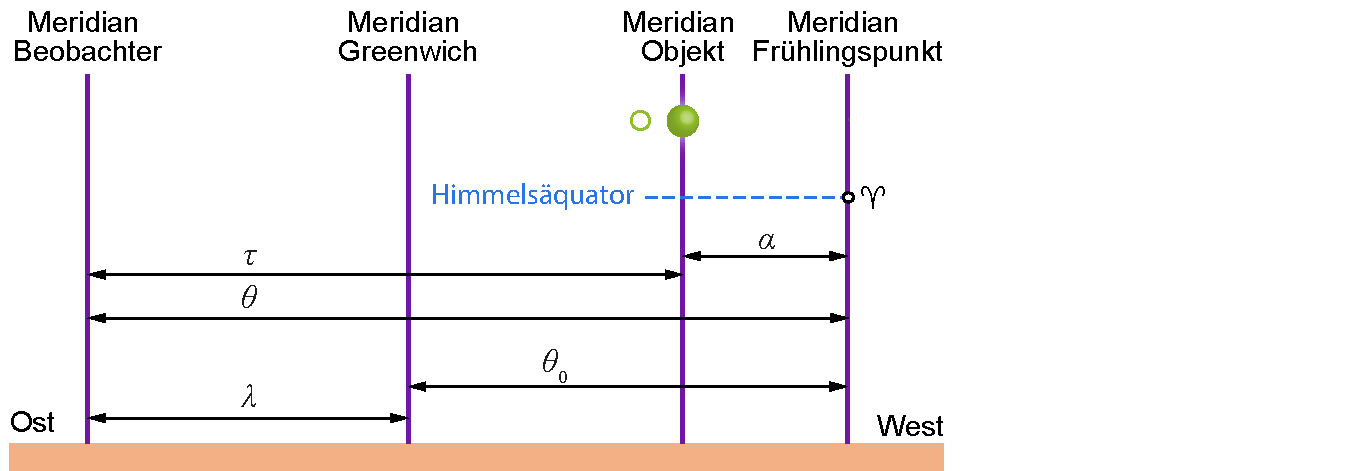
\includegraphics[width=\textwidth]{Vgl_Sternzeit_Tau.pdf}%
\caption[Sternzeit, Rektaszension, Stundenwinkel und geographische L�nge.]{Zusammenhang zwischen Sternzeit, Rektaszension, Stundenwinkel und geographischer L�nge.}%
\label{abb:hm_Sternzeit_Stundenwinkel}%
\end{figure}
Man verdeutliche sich dies anhand von \figref{hm_Sternzeit_Stundenwinkel}.
Die Sternzeit ist f�r alle Beobachter, die sich auf demselben L�ngengrad\index{L�ngengrad} $\lambda$ befinden, gleich gro� und ist damit eine Ortszeit.
Die (mittlere) Sternzeit des Referenzortes Greenwich G ist die Mittlere Greenwich Sternzeit GMST $\theta_0$ (\emph{engl.} Greenwich Mean Sidereal Time)\glslink{gmst}.
Die Ortssternzeit\index{Sternzeit!Orts-} $\theta$ am Beobachterort B wird mit LMST (\emph{engl.} Local Mean Sidereal Time) bezeichnet und berechnet sich mit dem L�ngengrad $\lambda$ (in \textdegree) wie folgt aus der GMST:
\begin{equation}
\text{LMST} = \theta = \text{GMST} + \lambda\,\frac{24 ^\text{h}}{360\degree}  = \theta_0 + \frac{\lambda}{15} \lk \frac{^\text{h}}{\degree} \rk \,. \label{eq:hm_LMST}
\end{equation}
Umgekehrt folgt aus der Differenz der lokalen Sternzeit eines Ortes zur Sternzeit in Greenwich die geographische L�nge dieses Orts.
Eine Messung dieser lokalen Sternzeit, \zb durch Bestimmung der Kulmination eines Sterns mit bekannter Rektaszension, entspricht daher einer geographischen Ortung, wenn die mittlere Greenwich Sternzeit bekannt ist (Beispiel \ref{bsp:laengengrad_abst_fl}).


%BEISPIEL 1 %%%%%%%%%%%%%%%%%%%%%%%%%%%%%%%%%%%%%%%%%%%%%%%%%%%%%%%%%%%%%%%%%%%%%%%%%%%%%%%%%
\begin{example}{Bestimmung von L�ngengrad und Abst�nden auf sph�rischen Fl�chen}  
Es sollen die Unsicherheit der Bestimmung eines L�ngengrades auf See, der Winkelabstand zweier Himmelsk�rper und die k�rzeste Flugstrecke zwischen zwei St�dten auf der Erdoberfl�che berechnet werden.
\begin{enumerate}[(a)]
	\item \emph{Wir wollen die Unsicherheit der Bestimmung eines L�ngengrades auf See nach einer dreimonatigen Seereise unter der Annahme einer perfekten Kulminationsbestimmung eines Sternes und einer Gangungenauigkeit der mitgef�hrten Uhren (auf GMST gestellt) von $1$, $3$, $5\:$s pro Tag berechnen.} \\ 	\medskip 
	Wir bezeichnen die Gangungenauigkeit mit $\Delta g\!=\!1\:\text{s}$, $3\:\text{s}$ \bzw $5\:\text{s}$.
        Die Seefahrt von \ca 3 Monaten dauere n�herungsweise 100 Tage, was eine Uhren-Gesamtverz�gerung von $\Delta g_{\text{tot}}\!=\!100\:\text{s}$, $300\:\text{s}$ bzw. $500\:\text{s}$ gegen�ber einer perfekten (auf Sternzeit \anf{geeichten} Uhr) nach sich zieht.
        Aus \eqref{eq:hm_LMST} folgt durch Differenzenbildung
\begin{equation*}
\Delta\theta = \Delta g_{\text{tot}} = \frac{\Delta\lambda}{15\degree} \,.
\end{equation*}
Hierin sind $\Delta g$ in Stunden anzugeben.
Es folgt:
\begin{equation*}
\Delta\lambda\lek\degree\rek = \frac{15}{3600}\,\Delta g_{\text{tot}}\lek\text{s}\rek = \begin{cases} \ \approx 25' \\ \approx 75' = 1\degree 15' \\ \approx 125' = 2\degree 05' \end{cases}
\end{equation*}
Das sind schon betr�chtliche Abweichungen.
Auf dem �quator sind das im letzten Fall �ber $\SI{200}{\kilo\metre}$.
Das zeigt, vor welchem Problem die nautische Navigation lange Zeit stand.
Dies konnte erst befriedigend mit der Entwicklung hinreichend genauer Uhren durch John Harrison\indexp{Harrison, John} (1693--1776) gel�st werden.
Harrison war ein englischer Erfinder und Uhrmacher.
Seine mechanischen und schiffstauglichen Uhren erm�glichten erstmals pr�zise Zeitmessungen auf See und damit die genaue Bestimmung des L�ngengrades.
Man kann daher auch verstehen, dass lange Zeit versucht wurde, die Zeit \bzw L�ngenbestimmung auf See durch Messung sehr genau bekannter astronomischer Ereignisse vorzunehmen (Mondfinsternisse, Monddistanzen, Sternbedeckungen und Position der Jupitermonde, etc.).
Sehr anschaulich wird die dadurch erreichte L�sung des sogenannten "`L�ngenproblems"' in \cite{Dash2004} nacherz�hlt.\\
	\item \emph{Es soll der Winkelabstand zweier Himmelsk�rper bestimmt werden (Siehe \figref{hm_winkelabstand}. Man achte besonders auf die Situation, wenn der Winkelabstand nahe $0\degree$ bzw. $180\degree$ liegt!).} \\ 	\medskip 
Wir nehmen an, dass die Positionen der beiden Himmelsk�rper durch Deklination $\delta$ und Rektaszension $\alpha$ gegeben sind.
Dann k�nnen wir nach Tabelle \ref{tab:hm_astro_KOS} die Richtungen zu den Positionen der beiden Himmelsk�rper als Vektoren $\vec{r}_{1}$ und $\vec{r}_{2}$ schreiben:
	\begin{align*}
	\vec{r}_1\:=\:\lk \begin{array}{c} x_1 \\ y_1 \\ z_1 \end{array}\rk\!=\:\lk \begin{array}{c} \cos \delta_1\,\cos \alpha_1 \\ \cos \delta_1\,\sin \alpha_1 \\ \sin \delta_1 \end{array}\rk \ , ~
	\vec{r}_2\:=\:\lk \begin{array}{c} x_2 \\ y_2 \\ z_2 \end{array}\rk\!=\:\lk \begin{array}{c} \cos \delta_2\,\cos \alpha_2 \\ \cos \delta_2\,\sin \alpha_2 \\ \sin \delta_2 \end{array}\rk  ~.
	\end{align*}
	Der Winkelabstand $\gamma$ ist dann einfach �ber das Skalarprodukt berechenbar:
	\begin{equation*}
	\gamma \:=\:\arccos \lk \:x_1 \; x_2\:+\:y_1 \, y_2\:+\:z_2\, z_2\:\rk \ ~.
	\end{equation*}
Bei Winkelabst�nden nahe $0\degree$ und nahe $180\degree$ erh�lt man nur sehr ungenaue Werte, da der Kosinus dort nahezu konstant ist.
\begin{center}
	  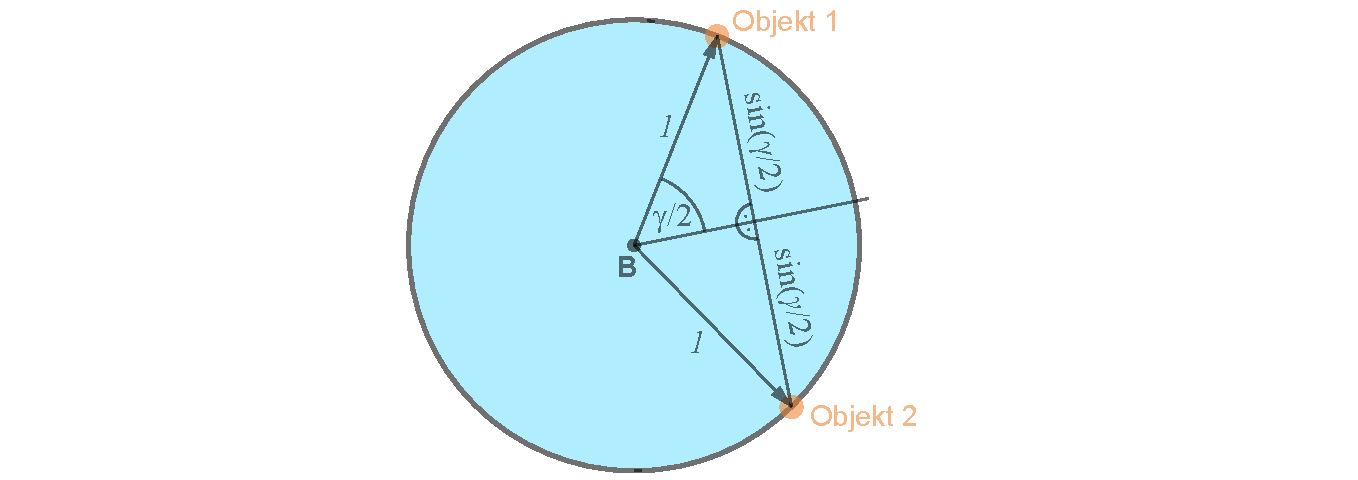
\includegraphics[width=0.75\columnwidth]{Winkelabstand.pdf}
\captionof{figure}{Winkelabstand zweier Himmelsk�rper.}\label{abb:hm_winkelabstand}
\end{center}
Man verwendet dann eine andere Formel.
Mit der L�nge des Differenzvektors $ d=\left|\vec{r}_1- \vec{r}_2\right| = \sqrt{(x_1-x_2)^2+(y_1-y_2)^2+(z_1-z_2)^2}$ ergibt sich dann 
$\gamma =\arcsin \lk \frac{d}{2} \rk $.\\
Bei Winkeln nahe $180\degree$ hat man immer noch ein Problem, da dort der Sinus des halben Winkels nahezu konstant ist.
Das l�st man dadurch, dass man den Winkelabstand $\bar{\gamma}$ von einem Objekt zum Antipoden des anderen berechnet.
Dieser Wert ist ja exakt um $180\degree$ verschoben, sodass $\bar{\gamma}$ wieder nahe bei $0\degree$ liegt.\\
	\item \emph{Es soll die k�rzeste Flugstrecke von St.~Petersburg (P) nach San Francisco (F) nahe der Erdoberfl�che berechnet werden (\figref{hm_Flug_SFO}, Geographische Breiten $\varphi_{\text{P}}=59.9\degree$, $\varphi_{\text{F}}=37.8\degree$ und geographische L�ngen $\lambda_{\text{P}}=30.3\degree$, $\lambda_{\text{F}}=-122.4\degree$), ebenso wie Anfangs- und Endkurs des Flugzeugs.}\\ 	\medskip 
Wir berechnen wieder den Winkelabstand zwischen den Punkten P und F.
Die k�rzeste Strecke ist dann -- wenn die Abplattung der Erde und die Flugh�he vernachl�ssigt werden -- der Abschnitt des Gro�kreises, der durch den Winkelabstand $\gamma$ definiert wird (siehe Abbildung):
$\overline{\text{PF}}=R_{\earth} \,,\gamma$, wobei $\gamma$ sich wie eben dargestellt berechnet.
Setzt man die Werte ein, erh�lt man $\overline{\text{PF}} \approx \SI{8867}{\kilo\metre}$.
Alternativ kann man die Berechnung nat�rlich �ber den Seiten-Kosinussatz der sph�rischen Trigonometrie machen.

\begin{center}

\includegraphics[width=\columnwidth]{Flug_SFO.pdf} \\ 
\captionof{figure}[Berechnung der k�rzesten Flugbahn zwischen zwei Orten.]{Berechnung der k�rzesten Flugbahn zwischen zwei Orten entlang der Erdoberfl�che.}\label{abb:hm_Flug_SFO} 
\end{center}

Die Anfangs- und Endkurse k�nnen wir mit dem Sinussatz aus dem Kugeldreieck $\Delta \text{F-NP-P}$ bestimmen, wobei wir die relative Richtung zu $N\!=\!360 \degree$ berechnen wollen:
\begin{align*}
	\sin\beta &=  \frac{\sin \lk \lambda_{\text{F}}-\lambda_{\text{P}} \rk}{\sin \gamma} \, \sin \lk 90 \degree - \varphi_{\text{F}} \rk ~~
	\Rightarrow \text{Kurs}_A = 360\degree - \beta \approx 338\degree ~~ \text{Anfangskurs und} \\
	\sin\alpha &=  \frac{\sin \lk \lambda_{\text{F}}-\lambda_{\text{P}} \rk}{\sin \gamma} \, \sin \lk 90 \degree - \varphi_{\text{P}} \rk ~~
	\Rightarrow \text{Kurs}_E = 180\degree + \alpha \approx 194\degree ~\text{Endkurs}.
\end{align*}
\end{enumerate} \label{bsp:laengengrad_abst_fl} 

\end{example}
%BEISPIEL %%%%%%%%%%%%%%%%%%%%%%%%%%%%%%%%%%%%%%%%%%%%%%%%%%%%%%%%%%%%%%%%%%%%%%%%%%%%%%%%%%

Mit der Sternzeit kommen wir direkt zur (wahren) \emph{Sonnenzeit}\index{Sonnenzeit!wahre} und k�nnen damit tats�chlich die b�rgerliche Zeit definieren \bzw genau messen.
Die Sonnenzeit ist wie die Sternzeit eine lokale Zeit.
Die Sternzeit ist 0 Uhr, wenn der Fr�hlingspunkt im Meridian steht.
Analog ist die Sonnenzeit 12 Uhr (mittags), wenn die Sonne den Ortsmeridian durchl�uft.
Man kann auch sagen, dass die Ortszeit der um 12 Stunden ($180\degree$) erh�hte Stundenwinkel der Sonne ist.
Die so definierte mittlere Ortszeit von Greenwich wird jetzt UT genannt und ist der um 12 Stunden erh�hte Stundenwinkel der fiktiven mittleren Sonne\index{Sonnenzeit!mittlere} in Greenwich\footnote{Die Addition von 12 Stunden ist n�tig, weil der Meridiandurchgang der fiktiven mittleren Sonne um 12:00 UT stattfinden soll, ihr Stundenwinkel in diesem Augenblick aber 0 betr�gt.}, \dh
\begin{equation}
\UT = 12\:\text{h} + \tau_\text{0, m. Sonne} \,.
\label{eq:hm_UT}
\end{equation} 
F�r Orte auf einem L�ngengrad $\lambda$ (in $\degree$) gilt analog zu \eqref{eq:hm_LMST}
\begin{equation}
\MOZ = \UT+ \frac{\lambda}{15} \lk \frac{\text{h}}{\degree} \rk \,.
\label{eq:hm_MOZ}\
\end{equation}
Die so definierte Sonnenzeit ergibt einen Sonnentag, der als Basis unserer Alltagszeit UT etwas l�nger ist als der oben definierte Sterntag. Die eigene Bewegung der Erde um die Sonne f�hrt dazu, dass die Zeit, bis die Sonne wieder kulminiert, etwas l�nger ist als die Zeit zwischen zwei Fixstern-Meridian-Durchg�ngen.
Nach einfacher Rechnung (Beispiel~\ref{bsp:sonnentag_sternentag}) findet man, dass der Sterntag gemessen an den 86400 (SI)-Sekunden des Sonnentags nur 23 Stunden, 56 Minuten und 4.0905 (SI)-Sekunden = 86125 (SI)-Sekunden lang ist.\footnote{Der Sterntag wird wieder in 24 Stunden unterteilt, die wir aber aus nachvollziehbaren Gr�nden und Respekt vor der Weltliteratur Stefan Zweigs hier nicht Sternstunden nennen.} % auskommentiert: hier gibt es keine Analogie. Genauso wenig bezeichnet ein Sonnentag einen Tag, an dem die Sonne scheint.}
Die Lage der fiktiven mittleren Sonne auf dem Himmels�quator kann nat�rlich nicht durch Beobachtung, sondern nur durch Rechnung bestimmt werden.
Nach \eqref{eq:hm_std_winkel_tau} gilt f�r den Meridiandurchgang der mittleren Sonne
\begin{equation}
\UT = 12\:\text{h} + \tau_\text{0, m. Sonne} = 12\:\text{h} + \theta_0 - \alpha_\text{0, m. Sonne} \,.
\label{eq:hm_UT_2}
\end{equation}

%BEISPIEL 2 %%%%%%%%%%%%%%%%%%%%%%%%%%%%%%%%%%%%%%%%%%%%%%%%%%%%%%%%%%%%%%%%%%%%%%%%%%%%%%%%%%
\begin{example}{Sonnentag und Sterntag}
  Wir wollen das Verh�ltnis von Sonnentag und Sterntag berechnen.
  Aus \figref{hm_Sterntag_Sonnentag} erkennt man, dass $\alpha\!=\!360\degree / n_\text{\astrosun}$, wobei $n_\text{\astrosun}$ die Zahl der Sonnentage pro tropischem Jahr bezeichnet. Das Verh�ltnis der Tagesl�ngen von Sonnentag $\text{d}_\text{\astrosun}$ zu Sterntag $\text{d}_\diamond$ ist dann:
\begin{equation*}
\frac{\text{d}_\text{\astrosun}}{\text{d}_\diamond} = \frac{360\degree + \frac{360\degree}{n_\text{\astrosun}}}{360\degree} = 1+\frac{1}{n_\text{\astrosun}} = 1+\frac{\text{d}_\text{\astrosun}}{\tau_\text{trop}} = \lk 1-\frac{\text{d}_\diamond}{\tau_{\text{trop}}} \rk^{-1}\,.
\end{equation*}
\begin{center}
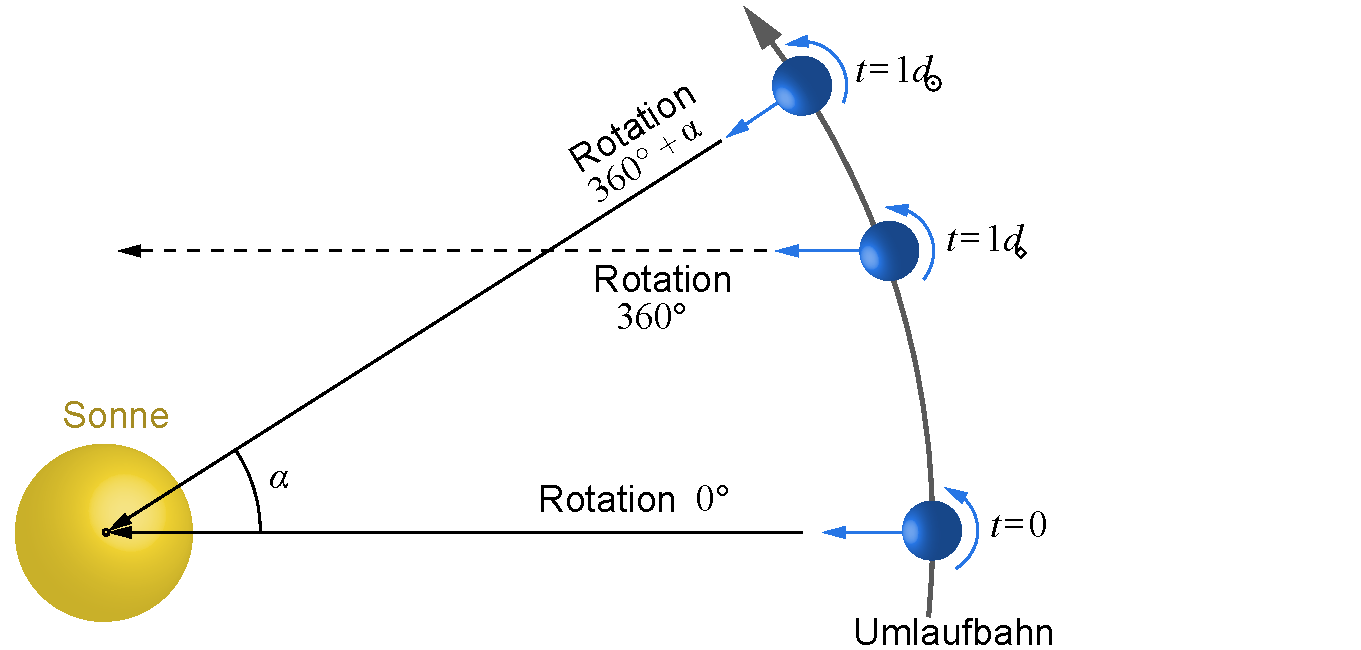
\includegraphics[width=0.8\columnwidth]{Sterntag_Sonnentag.pdf}% 
\captionof{figure}{Zum Unterschied zwischen Sterntag und Sonnentag.}\label{abb:hm_Sterntag_Sonnentag}
\end{center}
Mit $n_{\text{\astrosun}}\!=\! \frac{\tau_\text{trop}}{\text{d}_{\text{\astrosun}}} \! = \!365.242199 $ folgt daraus ${\text{d}_\text{\astrosun}}/{\text{d}_\diamond}\!=\!1.0027379$.
Der Sterntag ist damit um rund $1/365$ k�rzer als ein mittlerer Sonnentag und betr�gt $23$ Stunden $56$ Minuten und $4.0905$ Sekunden. \\

\label{bsp:sonnentag_sternentag}
\end{example}
%BEISPIEL %%%%%%%%%%%%%%%%%%%%%%%%%%%%%%%%%%%%%%%%%%%%%%%%%%%%%%%%%%%%%%%%%%%%%%%%%%%%%%%%%%

Auf Basis von \eqref{eq:hm_UT_2} wurde der Zusammenhang zwischen Weltzeit\index{Weltzeit} UT und der Greenwich Sternzeit\index{Greenwich Sternzeit} $\theta_0\!=\!\GMST(\UT)$ (\textit{Greenwich Mean Sideral Time})\index{Greenwich Mean Sideral Time} wie folgt festgelegt:
\begin{align} \label{eq:hm_UT_3}
\theta_0(\UT) =&\, 24110.5481\:\text{s}+8640184.812866\:\text{s}\, T_0+0.093104\:\text{s}\, T^2  \\
							 &+\mathcal{O}(T^3) + 1.0027379093\, \UT \nonumber \,,\\
\text{mit } T_0 = &\frac{\text{JD}_0-2451545.0}{36525}~~\text{und}~~T=\frac{\text{JD}-2451545.0}{36525}\,. \nonumber
\end{align}
Dabei sind $T_0$ und $T$ durch das jeweilige Julianische Datum um 0:00 des Beobachtungsdatums ($\text{JD}_0$) bzw. zur Uhrzeit des Beobachtungszeitpunkts (JD) gegeben.
Der lineare Term in \eqref{eq:hm_UT_3} gibt die Geschwindigkeit der fiktiven mittleren Sonne bez�glich des mittleren Fr�hlingspunkts an.
Das entspricht also multipliziert mit der Zeit einer Rektaszension.
Der quadratische Term ber�cksichtigt die weiter oben bereits erw�hnte pr�zessionsbedingte Bewegung des Fr�hlingspunkts.
Der Faktor $1.0027379093$ ergibt sich aus dem Unterschied zwischen Sonnentag  und Sterntag (Beispiel \ref{bsp:sonnentag_sternentag}).\footnote{Die L�nge des Sonnentages wird auch synodische Tagesl�nge\index{Periode!synodische}, die des Sterntages siderische Tagesl�nge\index{Periode!siderische} genannt.}
Gleichung \eqref{eq:hm_UT_3} stellt also einen Zusammenhang zwischen der Sternzeit und der Weltzeit UT her.
Obwohl die Weltzeit UT ihrer Definition gem�� eigentlich vom Sonnenlauf abzuleiten w�re, wird sie jedoch �ber \eqref{eq:hm_UT_3} aus den beobachteten Meridiandurchg�ngen von Sternen, also der Sternzeit, abgeleitet.
Das ist sinnvoll, da sich Sterndurchg�nge wesentlich pr�ziser beobachten lassen als die Position der �beraus hellen Sonne.
Man kann die Formeln aber nat�rlich auch benutzen, um die Sternzeit aus UT zu berechnen.

Nach diesen beiden mit einigen Definitionen versehenen Kapiteln haben wir nun die geeigneten Werkzeuge (Koordinatensysteme und Zeitdefinitionen), um die Mechanik der Himmelsk�rper beschreiben und vor allem auch Beobachtungsdaten ableiten \bzw berechnen zu k�nnen.
In der Himmelsmechanik wird im Grunde nichts anderes gemacht, als das Anfangswertproblem der entsprechenden Bewegungsgleichung f�r den oder die jeweiligen Himmelsk�rper  (Planeten, Monde, Kometen \ua) zu l�sen.
Die Bewegungsgleichung wollen wir nun als n�chstes aus den Gravitationsgesetzen herleiten. 
Wir werden dabei zun�chst allgemein, \dh ohne die Verwendung eines spezifischen Koordinatensystems, vorgehen.
Erst wenn wir Beobachtungsdaten und Ereignisse konkret berechnen, benutzen wir das jeweils passende r�umliche KOS.




\section{Bewegungsgleichung der Himmelsmechanik}\label{kap:hm_bewegungsgl}

In diesem Kapitel kommen wir zur grundlegenden Bewegungsgleichung der Himmelsmechanik.
In der Theorie der Gravitation ist die einfachste Konstellation eine aus zwei K�rpern, das sogenannte \emph{\gls{zkp}}\index{Zweik�rperproblem|textbf} (ZKP) (siehe Kapitel Physik der Bewegung im Band I). 
%Eine Bewegungsgleichung f�r das Zweik�rperproblem ist dabei eine Gleichung zur Bestimmung der Koordinaten der beiden K�rper im Raum als Funktion der Zeit.
Die entsprechende Bewegungsgleichung der Himmelsmechanik hei�t \emph{Kepler-Gleichung}.\index{Kepler-Gleichung|textbf}\indexp{Kepler, Johannes}\footnote{Johannes Kepler (1571 -- 1630 ) war ein deutscher Astronom und Physiker. Er entdeckte die Gesetzm��igkeiten, nach denen sich Planeten um die Sonne bewegen, die nach ihm benannten Keplerschen Gesetze, womit er zu den Begr�ndern der modernen Naturwissenschaften geh�rt. Wir schreiben wie sonst im Buch auch entsprechend der verwendeten Notation \emph{Kepler-Gleichung}, analog Lagrange-Gleichung, Euler-Gleichung usw. In der Astronomie hat sich historisch \emph{Keplergleichung} als  Konvention herausgebildet.} 
Die Bewegungsgleichung der Himmelsmechanik hei�t \emph{Kepler-Gleichung}.\index{Kepler-Gleichung|textbf}\indexp{Kepler, Johannes}\footnote{Johannes Kepler (1571 -- 1630 ) war ein deutscher Astronom und Physiker. Er entdeckte die Gesetzm��igkeiten, nach denen sich Planeten um die Sonne bewegen, die nach ihm benannten Keplerschen Gesetze, womit er zu den Begr�ndern der modernen Naturwissenschaften geh�rt. Wir schreiben wie sonst im Buch auch entsprechend der verwendeten Notation \emph{Kepler-Gleichung} (analog Lagrange-Gleichung, Euler-Gleichung usw.). In der Astronomie hat sich aber historisch \emph{Keplergleichung} als  Konvention herausgebildet.} 
Obwohl sie f�r die Himmelsmechanik eine fundamentale Bedeutung hat, wird die Kepler-Gleichung im Physik-Studium kaum behandelt.
Wir wollen sie deshalb hier zun�chst aus der Newtonschen Gravitationstheorie herleiten und auch eine auf Johannes Kepler selbst zur�ckgehende einfache geometrische Herleitung angeben.
Im Anschluss zeigen wir, wie man L�sungen f�r die Kepler-Gleichung erhalten kann und wie diese \zb f�r das Sonne-Erde- oder Sonne-Planeten-Problem aussehen.
Wir werden sp�ter auch sehen, dass dieser einfachen L�sungsansatz bereits f�r das Mond-Erde-System wegen der Einfl�sse der Sonne und der anderen Planeten  nicht mehr ausreicht.

\subsection{Herleitung der Kepler-Gleichung} \label{kap:hm_abl_kepler}
Die physikalischen Grundlagen der Bewegung des ZKP hatten wir uns bereits im Kapitel Physik der Bewegung im Band I angeeignet.
In \kap{hm_zeitdefinition} benutzten wir bei der Definition einiger KOS das Ergebnis, dass die Bewegung von Himmelsk�rpern in Bahnebenen stattfindet. Wir zeigen als Wiederholung noch einmal (diesmal in astronomischer Notation), dass sich die Bewegung in einer Ebene direkt aus der Tatsache ergibt, dass die Newtonsche Gravitationskraft eine Zentralkraft ist. 
Wir betrachten dazu das ZKP nach \figref{hm_2kp}, wobei wir den K�rper mit der Masse $M$ als wesentlich schwerer annehmen und deshalb als Zentralk�rper bezeichnen.
Den K�rper mit der wesentlich kleineren Masse $m$ wollen wir hingegen einfach Planet P nennen, obwohl es auch ein beliebiger anderer Himmelsk�rper (\zb Komet) sein kann.
Mit $\vec{r}_\text{M}$ und $\vec{r}_\text{m}$ bezeichnen wir die Vektoren vom Ursprung O eines beliebigen KOS zu den Massen $M$ \bzw $m$.
Der Vektor $\vec{r}=\vec{r}_\text{m}-\vec{r}_\text{M}$ zeigt vom Zentralk�rper zum Planeten.

\begin{figure}
\begin{minipage}{\textwidth}
\leftfigure{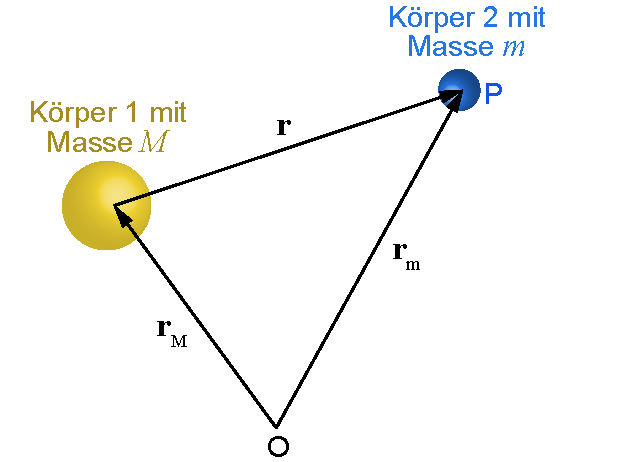
\includegraphics[width=0.5\textwidth]{ZKP.pdf}}
\hspace{\fill}
\rightfigure{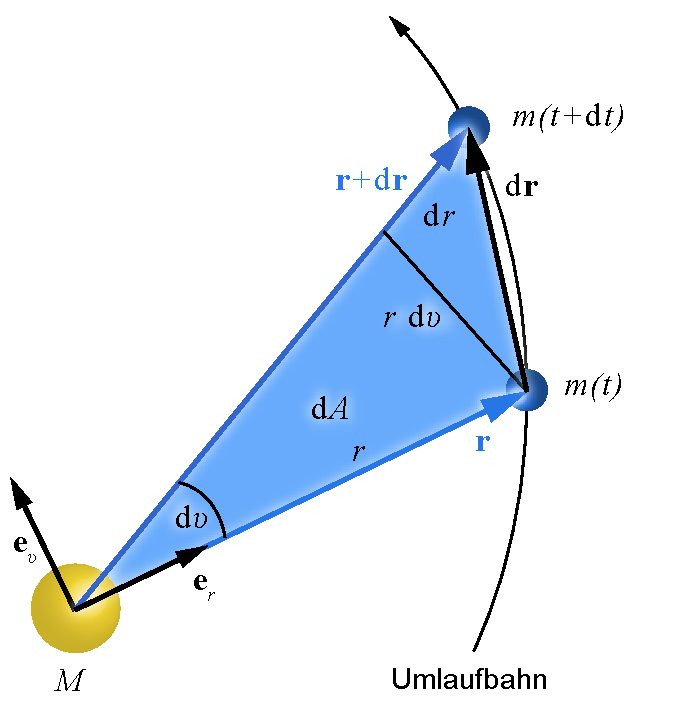
\includegraphics[width=0.5\textwidth]{Flaechensatz.pdf}}
\leftcaption{Zur Herleitung des Zweik�rperproblems.}\label{abb:hm_2kp}
\rightcaption{Fl�chensatz.} \label{abb:hm_flaechensatz}
\end{minipage}
\end{figure}

Laut Newtons Gravitationsgesetz\index{Gravitation} wirkt auf den K�rper mit der Masse $m$ (Planet) durch den Zentralk�rper mit der Masse $M$ (\zb die Sonne) eine Kraft
\begin{equation}
\vec{F}_\text{m} = m\,\ddot{\vec{r}}_\text{m} = -\frac{G \, M \, m}{r^3} \, \vec{r} \,.
\label{eq:hm_beschl_zk}
\end{equation}
Entsprechend wirkt auf den Zentralk�rper durch den Planeten die Kraft
\begin{equation}
\vec{F}_\text{M} = M\,\ddot{\vec{r}}_\text{M} = +\frac{G \, m \, M}{r^3} \, \vec{r} \,.
\label{eq:hm_beschl_pl}
\end{equation}
Die Beschleunigungen erh�lt man durch Division durch die Massen $m$ bzw. $M$:
\begin{equation}
\ddot{\vec{r}}_\text{m}-\ddot{\vec{r}}_\text{M} = \ddot{\vec{r}} = -\frac{G(M+m)}{r^3}\, \vec{r} = -\frac{\mu_\text{G}}{r^3}\, \vec{r}
\label{eq:hm_zk-pl}
\end{equation}
mit 
\begin{equation}
\mu_\text{G}\!=\!G\,(M+m). 
\label{eq:hm_def_muG}
\end{equation}
Hierin ist $G\!=\!\SI{6.673e-11}{\metre\cubed\per\kg\per\second\squared}$ die bereits in Band I eingef�hrte \emph{Gravitationskonstante}\glslink{gravkonst}.\index{Gravitationskonstante}\footnote{Man kann die Relativkoordinate auch so w�hlen, dass der Ort des Massenschwerpunkts $\vec{r}_\text{S}$ des Systems den Ursprung O des KOS bildet. Dann ist $\vec{r}_\text{S} = (M \vec{r}_\text{M} + m \vec{r}_\text{m})/(M+m)=0$ und die Bewegungsgleichung f�r den Planeten lautet $\ddot{\vec{r}} = -\mu_\text{G} \vec{r}/r^3 $ mit $\mu_\text{G}\!=\!GM (1 + m/M)^{-2}$, was f�r $ m \ll M$ in \eqref{eq:hm_def_muG} �bergeht.} %und $\mu_\text{G}$ der sogenannte \gls{gravparhm}.  
Zur eindeutigen L�sung von $\vec{r}(t)$ in \eqref{eq:hm_zk-pl} werden f�r das Differentialgleichungssystem 2.
Ordnung (in der Zeit) mit drei r�umliche Koordinaten folglich sechs Konstanten (Bewegungsintegrale \bzw Anfangsbedingungen) ben�tigt.
Wir wollen diese im Folgenden einzeln bestimmen. 

\subparagraph{\textbf{Drehimpulsintegral:}}\index{Drehimpulsintegral}
Wir beginnen mit der Herleitung des Drehimpulsintegrals\index{Drehimpulsintegral} und bilden dazu das Kreuzprodukt von $\vec{r}$ mit \eqref{eq:hm_zk-pl}:
\begin{equation*}
\vec{r} \times \ddot{\vec{r}} = -\frac{\mu_\text{G}}{r^3}\,  \vec{r} \times \vec{r} = 0 \,.\\
\end{equation*}
Es gilt aber auch
\begin{equation*}
\frac{\D }{\D t} \lk \vec{r} \times \dot{\vec{r}}\rk = \underbrace{\dot{\vec{r}} \times \dot{\vec{r}}}_{=0} + \underbrace{\vec{r} \times \ddot{\vec{r}}}_{=0} = 0 \; ,
\end{equation*}
woraus nach Integration sofort 
\begin{equation}
\vec{r} \times \dot{\vec{r}} = \vec{L} = \vec{const} 
\label{eq:hm_kepler1}
\end{equation}
folgt.
Der in \eqref{eq:hm_kepler1} definierte konstante Vektor $\vec{L}$ ist (bis auf den Faktor $m$ bzw. $m_\text{eff}$) gleich dem \gls{drehimpuls} des Planeten in Bezug auf den Zentralk�rper.
Er wird daher auch als \emph{spezifischer} Drehimpuls bezeichnet und ist also eine Konstante.
Gleichung \eqref{eq:hm_kepler1} wird daher als Drehimpulsintegral bezeichnet.
Wir werden ab jetzt wie in der Himmelsmechanik und Astronomie �blich die spezifischen Gr��en\footnote{H�ufig benutzt man auch f�r die spezifischen Gr��en Kleinbuchstaben oder griechische Symbole, also \zb f�r den Drehimpuls $\vec{l}$ \bzw $\vec{\lambda}$ anstelle $\vec{L}$. Wir bleiben aber im Folgenden bei den Gro�buchstaben, die auch den historisch in der Astronomie eingef�hrten Bezeichnungen und Symbolen entsprechen.} verwenden, man spart sich damit etwas Schreibarbeit und die Gleichungen werden �bersichtlicher.
Das ist im �brigen ein in der Physik �bliches Vorgehen, bei dem aber immer etwas Aufmerksamkeit angesagt ist.
Wir haben deshalb den Zusammenhang zwischen
den \anf{physikalischen} Gr��en aus Kapitel 1 (Band I)
und den hier verwendeten astronomischen Gr��en in Tabelle \ref{tab:hm_notation_hm} gelistet.%
\footnote{Es sei noch erw�hnt, dass \eqref{eq:hm_kepler1}
nur dann den spezifischen Drehimpuls des Planeten darstellt,
wenn dessen Masse sehr viel kleiner als die Masse
des Zentralk�rpers ist.
Im Fall $M\!\approx\!m$ gibt $\vec{L}$ nicht mehr
den Drehimpuls eines einzelnen K�rpers an.}
Da $\vec{L}$ senkrecht zu $\vec{r}$ und $\dot{\vec{r}}$
und konstant ist, findet die Bewegung in einer Ebene statt.
Dies ist eine der Aussagen des \emph{1.~Keplerschen Gesetzes}.
Aus der Konstanz des Drehimpulses $\vec{L}$ folgt sofort auch das \emph{2.~Keplersche Gesetz} (Fl�chensatz), da $\abs{\vec{r}\times\dot{\vec{r}}\,\D t}\!=\!\abs{\vec{r}\times\D \vec{r}}$ der doppelten Fl�che des von den Vektoren $\vec{r}$ und $\D \vec{r}$ aufgespannten Dreiecks entspricht.
Das ist aber gleich der Fl�che $\D A$, die von $\vec{r}$ in der Zeit $\D t$ �berstrichen wird (siehe \figref{hm_flaechensatz}). 

Wegen der Bewegung in einer Ebene sind f�r die Behandlung vieler Probleme Polarkoordinaten vorteilhaft.
Wir geben deshalb vielfach neben der vektoriellen Darstellung auch die Formulierung in Polarkoordinaten an.
Aus \figref{hm_flaechensatz} k�nnen wir direkt die ersten Ableitungen der (zeitabh�ngigen) Einheitsvektoren $\vec{e}_r$ und $\vec{e}_{\upsilon}$ ablesen (Drehung um den Ursprung mit Winkel $\D \upsilon$.):
\begin{equation*}
\dot{\vec{e}}_r \! = \dot{\upsilon} \, \vec{e}_{\upsilon}  ~\;\text{und} \;\dot{ \vec{e}}_{\upsilon} = -\dot{\upsilon} \, \vec{e}_{r} \,.
\end{equation*}
Hieraus bestimmt sich aus $\vec{r}\!=\!r\, \vec{e}_r$ und $\D \vec{r}\! = \!\D r \, \vec{e}_r + r\,\D  \upsilon \, \vec{e}_{\upsilon} $ die Geschwindigkeit $ \dot{\vec{r}}$ sofort zu 
\begin{align}
\dot{\vec{r}}\! = \!\vec{v}\!=\!\dot{r}\, \vec{e}_r + r\dot{\upsilon}\,\vec{e}_{\upsilon} ~. \label{eq:hm_vectoren_polar}
\end {align}
Nochmalige Anwendung der Differentiation auf $\dot{\vec{r}}$ f�hrt zu
\begin{equation}
\ddot{\vec{r}}\! =\!(\ddot{r}-r\dot{\upsilon}^2)\,\vec{e}_r + (2 \dot{r}\dot{\upsilon}+r\ddot{\upsilon})\,\vec{e}_{\upsilon} . \label{eq:hm_beschl_polar}
\end{equation}
Damit k�nnen wir den Drehimpuls und seinen Betrag schreiben:
\begin{equation}
\vec{L} = \vec{r}\times\dot{\vec{r}} = r^2 \dot{{\upsilon}} \veceZ \; , \label{eq:hm_drehimp_z}
\end{equation}
\begin{equation}
L=r^2\dot{\upsilon} ~. \label{eq:hm_drehimp_z_polar}
\end{equation}

\subparagraph{\textbf{Energieintegral:}}\index{Energieintegral}
Als N�chstes wollen wir ein Ma� f�r die \glslink{energie}{Gesamtenergie}\index{Energieintegral} des ZKP bestimmen.
Da das System konservativ ist, muss diese ja eine Erhaltungsgr��e sein.
Dazu bilden wir das Skalarprodukt von $\vec{v}\!=\!\dot{\vec{r}}$ mit $\ddot{\vec{r}}$:
\begin{align}
\begin{split}
\vec{v} \cdot \dot{\vec{v}} &= \vec{v} \cdot \ddot{\vec{r}} = -\frac{\mu_\text{G}}{r^3}\,\vec{v} \cdot \vec{r} = -\frac{\mu_\text{G}}{r^3}\,\dot{\vec{r}} \cdot \vec{r}  \\
 &= -\mu_\text{G} \frac{\dot{r}r}{r^3} = -\mu_\text{G} \frac{\dot{r}}{r^2} = \mu_\text{G}\,\frac{\D }{\D t} \lk \frac{1}{r}\rk \,.
\end{split} \label{eq:hm_v_mal_vpunkt_1}
\end{align}
Andererseits gilt
\begin{equation}
\vec{v} \cdot \dot{\vec{v}} = \frac{\D }{\D t} \lk \frac{v^2}{2} \rk \label{eq:hm_v_mal_vpunkt_2} .\\
\end{equation}
Daraus folgt mit {\eqref{eq:hm_v_mal_vpunkt_1}
\begin{equation}
\frac{\D }{\D t} \lk \frac{v^2}{2} - \frac{\mu_\text{G}}{r}\rk = 0 \label{eq:hm_v_mal_vpunkt_3}
\end{equation}
und nach Integration
\begin{equation}
\frac{v^2}{2} - \frac{\mu_\text{G}}{r} = H = \con\:. \label{eq:hm_bewgl1}
\end{equation}
Auf der linken Seite von \eqref{eq:hm_bewgl1} steht die durch $m$ dividierte Summe aus kinetischer und \glslink{potential-hm}{potentieller Energie} des umlaufenden K�rpers.
Diese Summe $H$ ist wie erwartet f�r ein konservatives System\index{System!konservatives} konstant.\footnote{Wir verwenden den Buchstaben $H$ f�r die Energie, da die ansonsten �bliche Bezeichnung $E$ aus historischen Gr�nden f�r die weiter unten eingef�hrte exzentrische Anomalie reserviert ist.}
Man erkennt aus dem Energieintegral ferner, dass f�r $H\!<\!0$ die Bewegung r�umlich beschr�nkt sein muss.
Damit $\mu_\text{G}/r\!>\!v^2/2$ bleibt, kann $r$ nicht unendlich werden.

\subparagraph{\textbf{Laplace-Integral (Richtungsintegral):}}\index{Laplace-Integral}\index{Richtungsintegral}\indexp{Laplace, Pierre-Simon (Marquis) de}

Wir bilden nun noch das Vektorprodukt aus $\vec{L}$ und $\ddot{\vec{r}}$:
\begin{equation*}
\vec{L} \times \ddot{\vec{r}} = \lk \vec{r} \times \dot{\vec{r}}\rk \times \lk \frac{-\mu_\text{G}}{r^3} \rk\, \vec{r} \,.
\end{equation*}
Man findet nach etwas Vektoralgebra (\probref{hm_laplace}) eine weitere Integrationskonstante, die wir als \emph{Laplace-Vektor}\index{Laplace-Vektor} $\vec{e}$ der Bewegung bezeichnen:
\begin{equation}
\vec{L} \times \dot{\vec{r}} + \lk \frac{\mu_\text{G}}{r} \rk \, \vec{r} = \vec{const} = -\mu_\text{G} \, \vec{e} \,. \label{eq:hm_laplace_int}
\end{equation}
Dieser Vektor, der in der (vor allem angels�chsischen) Literatur oft auch als Runge\footnote{Carl David Tolm� Runge (1856--1927) war ein deutscher Mathematiker, der auf zahlreichen Gebieten der Mathematik und mathematischen Physik forschte. In Band I hatten wir Runge bereits im Zusammenhang mit dem Runge-Kutta-Verfahren kennen gelernt.}-Lenz\footnote{Wilhelm Lenz (1888--1957) war ein deutscher Physiker, der an der Universit�t Hamburg lehrte und auf zahlreichen Gebieten der Physik aktiv war. Er f�hrte \ua den Runge-Lenz-Vektor in die Quantenmechanik ein.}-Vektor\index{Runge-Lenz-Vektor} bezeichnet wird, liegt in der Bahnebene und gibt eine Vorzugsrichtung innerhalb der Bahnebene vor.
Der Laplace-Vektor ist aber nicht v�llig unabh�ngig von den beiden anderen Bewegungsintegralen.
Man kann unter Benutzung von \eqref{eq:hm_kepler1} und \eqref{eq:hm_bewgl1} zeigen, dass $\vec{L}\cdot \vec{e}\!=\!0$ und dass demzufolge die Beziehungen
\begin{equation}
\mu_\text{G}^2 \, \lk \abs{\vec{e}}^2 - 1 \rk = 2H \, \abs{\vec{L}}^2 ~~~\text{\bzw}~~~~ e^2 = \frac{2H L^2}{\mu_\text{G}^2} + 1  
\label{eq:hm_relations1}
\end{equation}
gelten (\probref{hm_laplace}).
Der Betrag $\abs{\vec{e}}\!=\!e$ des Laplace-Vektors wird \emph{(numerische) Exzentrizit�t}\footnote{In der Mathematik wird die numerische Exzentrizit�t im Allgemeinen mit $\epsilon$ bezeichnet, w�hrend dort $e=\sqrt{a^2-b^2}$ f�r die lineare Exzentrizit�t steht.
Da $\epsilon$ in der Himmelsmechanik f�r die Neigung der Erdachse reserviert ist, bleiben wir bei der Nutzung von $e$ f�r die (numerische) Exzentrizit�t (siehe auch Tabelle \ref{tab:hm_notation_hm} im Tabellenanhang.)} genannt und ist nach \eqref{eq:hm_relations1} durch die Energie und den Drehimpuls vollst�ndig festgelegt.
\vec{e} liefert dann nur noch als unabh�ngige Gr��e einen Winkel bzw. eine Richtung.
Wir haben nun f�nf unabh�ngige Konstanten $\vec{L}$ (3 Komponenten), $H$ und die Richtung von $\vec{e}$ innerhalb der Bahnebene aus den Bewegungsintegralen gewonnen, die wir als physikalische Bahnparameter betrachten k�nnen.
Als sechsten Parameter nutzen wir eine Anfangsbedingung, \zb die Bahnposition des K�rpers zu einem bestimmten Zeitpunkt.
Wir arbeiten wieder mit den Polarkoordinaten $r$ und $\upsilon$, wobei wir die beliebig w�hlbare Bezugsrichtung des Polar-KOS in Richtung von $\vec{e}$ legen wollen.
Den Winkel $\upsilon$ zu dieser Bezugsachse wollen wir ab jetzt, wie in der Astronomie �blich, als \emph{wahre Anomalie}\index{Anomalie!wahre|textbf}\footnote{Der Begriff \anf{Anomalie} (\emph{altgriechisch} f�r Unebenheit, Unregelm��igkeit) geht auf die antiken Astronomen zur�ck, die den Winkel in der Bahnbewegung als abweichend und unregelm��ig von der erwarteten \anf{harmonischen} Kreisbahn beobachteten.
Historisch hat sich f�r die wahre Anomalie die Bezeichnung mit dem griechischen Buchstaben Ypsilon $\upsilon$ (\figref{hm_polarkoord}) herausgebildet.} bezeichnen.\\

\begin{figure}
\begin{minipage}{\textwidth}
\leftfigure{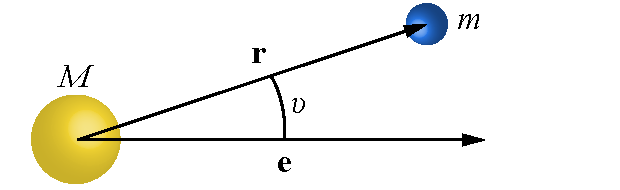
\includegraphics[width=0.5\textwidth]{Polarkoordinaten.pdf}}
\hspace{\fill}
\rightfigure{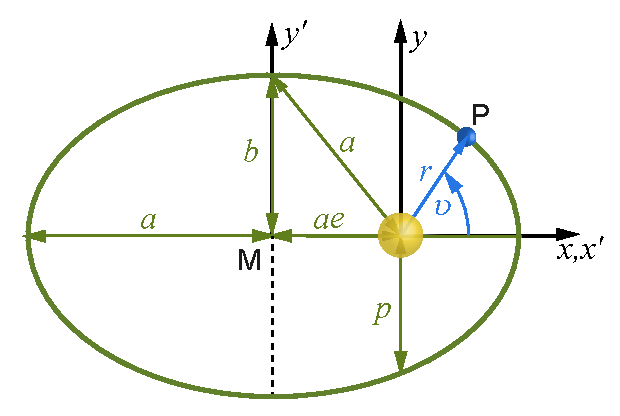
\includegraphics[width=0.5\textwidth]{Geometrie_der_Ellipse.pdf}}
\leftcaption{Polarkoordinaten.}\label{abb:hm_polarkoord}
\rightcaption[Geometrie der Ellipse.]{Geometrie der Ellipse. Man beachte die beiden Koordinatensysteme, das $x$-$y$-\KOS hat den Ursprung im Brennpunkt der Ellipse, das sogenannte Mittelpunkts-$x'$-$y'$-\KOS im Mittelpunkt.}\label{abb:hm_ellipse}
\end{minipage}
\end{figure}

Mit der Bezugsrichtung von $\vec{e}$ schreiben wir das Skalarprodukt $\vec{r} \cdot \vec{e}$ als
\begin{align}
\begin{split}
\vec{r} \cdot \vec{e} &= -\vec{r} \cdot \lk \frac{\vec{L}\times \dot{\vec{r}}}{\mu_\text{G}} + \frac{\vec{r}}{r} \rk \\
                      &= - \frac{\vec{r} \cdot ( \vec{L} \times \dot{\vec{r}} )}{\mu_\text{G}} - r = \frac{(\vec{r} \times \dot{\vec{r}}) \cdot \vec{L}}{\mu_\text{G}} - r = \frac{L^2}{\mu_\text{G}} - r = re\,\cos \upsilon \; ,
\end{split} \label{eq:hm_relations2}
\end{align}
woraus
\begin{align}
r(\upsilon) = \frac{L^2}{\mu_\text{G}}\,\frac{1}{1+e\,\cos \upsilon} = \frac{p}{1+e\,\cos \upsilon} \label{eq:hm_kegelschnitt}
\end{align}
folgt.
Wir haben damit f�r die Form der Bahn die Gleichung f�r Kegelschnitte\index{Kegelschnitt} erhalten.
Der sogenannte Halb-Parameter $p\!=\!L^2/\mu_\text{G}$ wird \emph{semi-latus rectum} genannt.
Dies ist der Abstand des Planeten zum Zentralk�rper bei einem Winkel $\upsilon = \pm\pi/2$ (\figref{hm_ellipse}).
Folgende Schlussfolgerungen kann man aus Gleichung \eqref{eq:hm_kegelschnitt} ziehen:
\begin{itemize}
	\item F�r $\cos\upsilon\!=\!1$ bzw. $\upsilon\!=\!0$, d.\,h. f�r die Richtung von $\vec{e}$, finden wir den Punkt der Bahn, der dem Zentralk�rper am n�chsten kommt.
          Dies ist die sogenannte \index{Periapsis}\emph{\gls{periapsis}} (im Fall der Sonne als Zentralk�rper das \index{Perihel|textbf}\emph{\gls{perihel}}).
          Damit wird der Begriff des Richtungsintegrals f�r den Laplace-Vektor verst�ndlich.
	\item F�r $\cos\upsilon\!=\!-1$ bzw. $\upsilon\!=\! \pi$, d.\,h. in entgegengesetzter Richtung von $\vec{e}$, erhalten wir den Punkt der Bahn, der dem Zentralk�rper am fernsten liegt.
          Dies ist die \index{Apoapsis}\emph{\gls{apoapsis}} (im Fall der Sonne als Zentralk�rper das \index{Aphel|textbf}\emph{\gls{aphel}}).
	\item F�r $\cos\upsilon\!=\!0$, also $\upsilon\!=\!\pm\pi/2$ ergibt sich $r\!=\!p$.
	\item F�r den Fall $0\!<\!e\!<\!1$ ergibt sich aus \eqref{eq:hm_relations2} als Bahn eine Ellipse.
          In diesem Fall ist auch nach \eqref{eq:hm_relations1} die Energie $H\!<\!0$. 
	\item F�r $e\!=\!1$ ergibt \eqref{eq:hm_kegelschnitt} eine Parabel und f�r $e\!>\!1$ eine Hyperbel.
          Wir sehen, dass die genaue Form der Bahn von den Parametern $L$ (Drehimpuls) und $e$ (Exzentrizit�t) und damit nach \eqref{eq:hm_relations1} auch von der Energie des Systems abh�ngt.
\end{itemize}
Wir wollen uns im Folgenden auf \emph{Ellipsenbahnen}\index{Ellipsenbahnen} (\figref{hm_ellipse}) beschr�nken.
F�r eine Ellipsenbahn wird die \glslink{groszehalbachse}{gro�e Halbachse} mit $a$ bezeichnet und die \glslink{kleinehalbachse}{kleine} mit $b$.
F�r $e$ gilt dann $0<e=\sqrt{1-\frac{b^2}{a^2}}<1$.
Damit ergeben sich f�r den kleinsten und den gr��ten Abstand des umlaufenden Planeten folgende Beziehungen:
\begin{align}
r_\text{min} &= \frac{L^2}{\mu_\text{G}} \frac{1}{1+e}~~\,, ~~r_\text{max} = \frac{L^2}{\mu_\text{G}} \frac{1}{1-e} \,. \label{eq:hm_aphel_perihel} 
\end{align}
Mit $r_\text{min}\!+\!r_\text{max}\!=\!2a$ folgt daraus
\begin{equation}
L = r^2\dot{\upsilon} = \sqrt{a\,\mu_\text{G}(1-e^2)} \,,  \label{eq:hm_drehimpuls_von_ae}
\end{equation}
womit wir einen Zusammenhang von physikalischen Bahnparametern ($L$) und geometrischen Parametern der Bahn ($a$, $e$) hergestellt haben.
Die Bahngleichung $r(\upsilon)$ schreiben wir dann mit den geometrischen Bahnparametern $a$ und $e$ in der �blichen Form:
\begin{equation}
r(\upsilon) = \frac{a(1-e^2)}{1+e\,\cos \upsilon} = \frac{p}{1+e\,\cos \upsilon}\,. \label{eq:hm_bahnglg}
\end{equation}
Wir leiten jetzt noch das \emph{3. Keplersche Gesetz} her, indem wir die Beziehung f�r den Drehimpuls \eqref{eq:hm_drehimpuls_von_ae} �ber die gesamte Ellipse, \dh �ber eine ganze Umlaufperiode $T_\text{P}$, integrieren:\footnote{Wir erinnern an die geometrische Interpretation des Drehimpulses als 2 $\D A /\D t$ im Rahmen der Herleitung des 2.\ Keplerschen Gesetzes.}
\begin{equation}
A = \frac{1}{2} \int\limits_0^{T_\text{P}} L\,\D t = \frac{1}{2}\, L\,T_\text{P} = \frac{1}{2}\sqrt{a \mu_\text{G}\lk 1-e^2\rk } \,T_\text{P} \,. \label{eq:hm_bahnglg_a}
\end{equation}
Andererseits ist der Fl�cheninhalt einer Ellipse $A\!=\!\pi a b\!=\! \pi a^2\sqrt{1-e^2}$.
Daraus folgt durch Quadrieren von \eqref{eq:hm_bahnglg_a} und Gleichsetzen mit \eqref{eq:hm_bahnglg}
\begin{equation}
\frac{T_\text{P}^2}{a^3} = \frac{4\pi^2}{\mu_\text{G}} = \con = \frac{4\pi^2}{GM} ~.
\label{eq:hm_3_kepler_gesetz}
\end{equation}
Die Quadrate der Umlaufperioden zweier Planeten um einen Zentralk�rper verhalten sich wie die Kuben ihrer gro�en Halbachsen. \\
Wir m�ssen hier eine Bemerkung zu der Umlaufzeit $T_\text{P}$ machen: Diese Zeit ist als siderische Umlaufzeit\glslink{siderischeumlaufzeit}\ definiert, \dh als die Zeit, die ein Planet f�r einen vollst�ndigen Umlauf braucht, um \zb die Sonne wieder vor dem gleichen Fixsternhintergrund zu sehen.
Diese Umlaufzeit l�sst sich aber nur f�r die Erde direkt bestimmen.
F�r alle anderen Planeten muss man sie aus der \glslink{synodischeumlaufzeit}{synodischen Umlaufzeit} berechnen.
Diese ergibt sich, wenn der andere Planet von der Erde aus betrachtet wieder im gleichen Winkelabstand zur Sonne steht.
Zum Gl�ck hatte Kepler sehr genaue Aufzeichnungen von Tycho Brahe\footnote{Tycho Brahe\indexp{Brahe, Tycho} (1546--1601) war ein bedeutender d�nischer Astronom. Seine Beobachtungen, die Kepler erst nach Brahes Tod auswertete, bildeten die Grundlage f�r die Ableitung der Keplerschen Gesetze (siehe auch \cite{Hecht2019}). Brahe f�hrt die Beobachtung vor gut 400 Jahren in der damals leistungsst�rksten Sternwarte der Welt auf der kleinen Insel Ven im �resund zwischen Kopenhagen und Malm� durch, wobei er mit exzellenten Winkelmessinstrumenten, aber ohne Teleskop arbeitete, das damals noch unbekannt war.}, die ihm die Berechnung der siderischen Umlaufzeit des Mars erm�glichten.
In \probref{hm_sideric_period_mars} kann die Berechnung Keplers f�r die Beobachtung von Mars-\glslink{opposition}{Oppositionen}\index{Mars-Opposition} nachvollzogen werden.
Bahnberechnungen f�r die Planeten unseres Sonnensystems sind im \mscr{} \mlhmref{InnerePlaneten.m} zu finden. 

\subparagraph{\textbf{vis-viva-Gleichung:}}
Wir wollen noch eine weitere wichtige Beziehung herleiten, und zwar die zwischen der Himmelsk�rperposition (Abstand zum Zentralk�rper) und seiner Bahngeschwindigkeit am jeweiligen Ort.
Diese Relation wird als \gls{visvivahm}\index{vis-viva-Gleichung}\footnote{Diese Formel wurde erstmalig von Gottfried Wilhelm Leibniz (1646--1716), einem der letzten gro�en Universalgelehrten, gefunden.} bezeichnet und ergibt sich, indem in \eqref{eq:hm_bewgl1} f�r $H$ die Gleichung \eqref{eq:hm_relations1} und f�r $L$ die Beziehung \eqref{eq:hm_drehimpuls_von_ae} eingesetzt wird. Wir erhalten die 
\begin{merksatz}  {vis-viva-Gleichung (\bzw den vis-viva-Satz)}
\begin{equation}
v^2 = \mu_\text{G} \lk \frac{2}{r} - \frac{1}{a} \rk \, \label{eq:hm_vis-viva}
\end{equation}\\

\end{merksatz}

und k�nnen damit zu jedem Punkt der Bahn (gegeben durch den Abstand $r$) die dort vorhandene Bahngeschwindigkeit $v$ bestimmen. 

In der Bahngleichung \eqref{eq:hm_bahnglg} stecken mit $a$ und $e$ nur zwei der sechs notwendigen Bahnparameter (Integrationskonstanten).
Das ist nicht verwunderlich, da wir uns ja mit den $r,\upsilon$-Koordinaten quasi in die Bahnebene \anf{gelegt} haben.
Zur vollen r�umlichen und zeitlichen Beschreibung der Bewegung muss diese Ebene noch im dreidimensionalen Raum positioniert und eine Anfangsbedingung festgelegt werden.
Dazu benutzt man, wie bereits in \kapitel{hm_koordinatensysteme} beschrieben, eine Bezugsebene und eine Bezugsrichtung, relativ zu denen die Bahnebene positioniert wird.
F�r unser Sonnensystem ist das sinnvollerweise das heliozentrisch-ekliptikale KOS, woraus sich drei weitere geometrische Bahnparameter, n�mlich $\omega$ (\glslink{argperiapsis}{Argument des \gls{perihel}s}), $\Omega$ (\glslink{laengeaufstknoten}{L�nge des \glslink{aufstknoten}{aufsteigenden Knotens}}\footnote{Alternativ zu $\Omega$ kann auch der Parameter $\varpi=\omega+\Omega$ verwendet werden. Bei dem aus historischen Gr�nden verwendeten Buchstaben $\varpi$ handelt es sich um eine Variante des griechischen $\pi$.}), und $i$ (Neigung der Bahn gegen die Ekliptik) ergeben (\figref{hm_bahnelemente}).
Mit den f�nf Bahnparametern $a$, $e$, $\omega$, $\Omega$ (bzw. $\varpi$), $i$ bezogen auf das heliozentrisch-ekliptikale KOS und dem Zeitpunkt des \textit{Periheldurchgangs} $t_0$ sind die Bahnen f�r ein ZKP vollst�ndig charakterisiert.
Die Bahnparameter unserer Planeten sind in Tabelle \ref{tab:hm_bahnparameter} im Tabellenanhang angegeben.
Die Exzentrizit�ten $e$ ihrer Bahnen sind meist gering, nur Merkur, Mars und Pluto haben eine etwas gr��ere Exzentrizit�t.
Was f�r ein Gl�ck, dass der Mars eine gr��ere Exzentrizit�t hat! So konnten Brahe und Kepler die elliptische Form der Marsbahn mit den damals verf�gbaren Methoden �berhaupt bestimmen.
Wir werden die Bahnelemente in \kapitel{kulmination_sonne} noch etwas ausf�hrlicher diskutieren. 

\begin{figure}
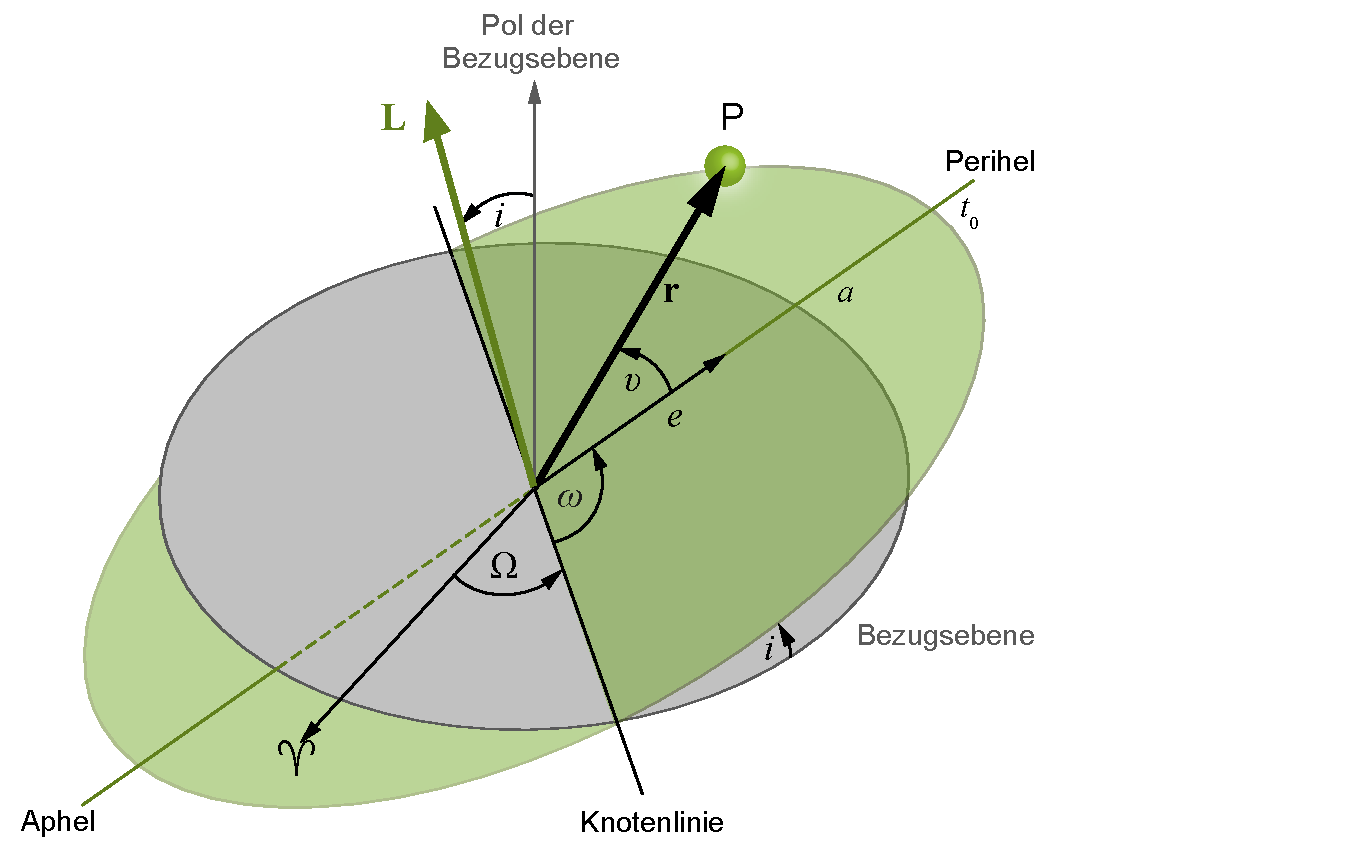
\includegraphics[width=\textwidth]{Bahnelemente2.pdf}%
\caption[Bahnelemente der Planeten im Sonnensystem.]{Bahnelemente der Planeten im Sonnensystem. $i$ bezeichnet die Inklination (Neigung der Bahn zur Ekliptik), $\Omega$ die L�nge des aufsteigenden Knotens, $\omega$ das Argument (den Winkel) des Perihels, $a$ die gro�e Halbachse, $e$ die Exzentrizit�t und $t_0$ die Periheldurchgangszeit. H�ufig wird auch die L�nge des Perihels $\varpi=\omega+\Omega$ angegeben.}
\label{abb:hm_bahnelemente}
\end{figure}

Bei Kenntnis der Bahnparameter\footnote{Man findet diese Bahnparameter an vielen Stellen, in astronomischen Jahrb�chern oder auch im Internet. Hier sei besonders auf die Seiten des \textit{\gls{jplhm}~(JPL)}\index{Jet Propulsion Lab (JPL)} auf \url{https://ssd.jpl.nasa.gov/?ephemerides} verwiesen.} im \glslink{ekliptkoord}{ekliptikalen System} kann man jederzeit mit den in Tabelle \ref{tab:hm_Umrechung_KOS} beschriebenen Transformationen die Bahnkoordinaten auch in jedem anderen KOS berechnen.\\
Wir sind aber nicht nur an der Form der Bahn, sondern insbesondere auch an dem zeitlichen Verlauf der Bewegung entlang der beschriebenen Bahn $r(\upsilon)$ interessiert, also an $r(t)$ bzw. an $\upsilon(t)$.
Die wahre Anomalie ist unserer Beobachtung wegen der gr��eren �nderung �ber die Zeit und einfacheren Messung von Winkeln relativ einfach zug�nglich.
Wir starten mit der Bahngeschwindigkeit in Polarkoordinaten
\begin{equation} \label{eq:hm_vis-viva_polar}
v^2 = \dot{r}^2 + r^2\dot{\upsilon}^2 = \dot{r}^2 + \frac{L^2}{r^2}  
\end{equation}
und setzen diesen Ausdruck in den vis-viva-Satz \eqref{eq:hm_vis-viva} ein.
Ebenso benutzen wir f�r $L$ die Beziehung \eqref{eq:hm_drehimpuls_von_ae} und erhalten  
\begin{align} \label{eq:hm_dot_r_quadrat} 
\dot{r}^2 &= \mu_\text{G} \lk \frac{2}{r} - \frac{1}{a} \rk - \frac{L^2}{r^2} = \mu_\text{G} \lk \frac{2}{r} - \frac{1}{a} - \frac{a(1-e^2)}{r^2} \rk \nonumber \\
					&= \frac{\mu_\text{G}}{r^2} \lk 2r - \frac{r^2}{a} - a\,(1-e^2) \rk\,.  
\end{align}
Jetzt f�hren wir die \gls{exzentranom} \index{Anomalie!exzentrische|textbf} $E(t)$ als Hilfsgr��e f�r die Berechnung von $r(t)$ ein: 
\begin{equation}
r(t) = a \,\lk 1-e\,\cos E(t)\rk \,.\label{eq:hm_exzentrische_Anomalie}
\end{equation}
Die mag zun�chst etwas formal-mathematisch erscheinen. Die geometrische Bedeutung von $E$ wird im \kapitel{deutung_kepler} klar werden.
Wir leiten \eqref{eq:hm_exzentrische_Anomalie} nach der Zeit ab
\begin{equation*}
\dot{r}(t) = \frac{\D r}{\D E} \frac{\D E}{\D t} = a\,e\,\sin E\, \frac{\D E}{\D t} \,,
\end{equation*}
setzen  dies in \eqref{eq:hm_dot_r_quadrat} ein und erhalten zun�chst
\begin{align*}
a^2\,e^2\,\sin^2 E \,\lk\frac{\D E}{\D t}\rk^2 &= \frac{\mu_\text{G}}{r^2} \,(a\,e^2 - a\,e^2\,\cos^2 E) = \frac{\mu_\text{G}}{r^2}\, a\,e^2 \,\sin^2 E\,. 
\end{align*}
Durch K�rzen von $a^2e^2\sin^2E$ und Wurzelziehen folgt
\begin{equation*}
r \lk \frac{\D E}{\D t} \rk = \sqrt{\frac{\mu_\text{G}}{a}} \,.%\label{eq:hm_r_dE_dt}
\end{equation*}
Mit der Definition der exzentrischen Anomalie \eqref{eq:hm_exzentrische_Anomalie} und Trennung der Variablen wird daraus
\begin{equation}
\lk 1-e\,\cos E(t) \rk \,\D E = \sqrt{\frac{\mu_\text{G}}{a^3}}\,\D t\,. \label{eq:hm_1-ecosEdE}
\end{equation}
Wir f�hren noch mit der Umlaufzeit $T_\text{P}$ \bzw der Umlaufwinkelgeschwindigkeit $n_\text{P}$ die \emph{mittlere Anomalie} $M$\glslink{mittlereanom} ein:
\begin{equation}
M = M(t) = \sqrt{\frac{\mu_\text{G}}{a^3}} \,(t-t_0) = \frac{2 \pi}{T_\text{P}}\,(t-t_0) = n_\text{P}\,(t-t_0) \,. \label{eq:hm_mittlere_anomalie}
\end{equation}
Nach Integration von \eqref{eq:hm_1-ecosEdE} �ber $\D E$ erhalten wir schlie�lich die ebenso ber�hmte wie kompakte \emph{Kepler-Gleichung}\index{Kepler-Gleichung}.
\begin{merksatz}{Kepler-Gleichung}
\begin{equation}
E-e\,\sin E = M  \,.\label{eq:hm_keplerglg}
\end{equation}\\

\end{merksatz}

Diese Gleichung wurde von Kepler\indexp{Kepler, Johannes} 1609 erstmals in seiner \anf{Astronomia Nova} \cite{Kepler1992} ver�ffentlicht.
Obwohl sie keine Differentialgleichung ist, handelt es sich tats�chlich um eine Bewegungsgleichung, denn auf beiden Seiten der Kepler-Gleichung stehen mit $M(t)$ und $E(t)$ zeitabh�ngige Gr��en.\footnote{Da wir Bewegungsintegrale bei der Herleitung von \eqref{eq:hm_keplerglg} verwendet haben, ist das Verschwinden der Ableitungen nach der Zeit nicht verwunderlich.
Eigentlich sollte man besser schreiben $E(t)-e\,\sin E(t)\!=\!M(t)$.} Die Bewegungsintegrale stecken in den (geometrischen) Parametern $e$ und $M$.
$M(t)$ ist durch die gro�e Halbachse $a$ oder nach dem 3.~Keplerschen Gesetz \eqref{eq:hm_3_kepler_gesetz} durch die Umlaufzeit $T_\text{P}$ gegeben.
Hat man �ber \eqref{eq:hm_keplerglg} $E(t)$ berechnet, kann man dann �ber \eqref{eq:hm_exzentrische_Anomalie} den Abstand $r(t)$ bzw. �ber \eqref{eq:hm_bahnglg} die wahre Anomalie $\upsilon(t)$ bestimmen. \\


\subsection{Geometrische Deutung und Ableitung der Kepler-Gleichung} \label{kap:deutung_kepler}

Wir wollen uns jetzt noch die Bedeutung der mittleren, wahren und exzentrischen \emph{Anomalien} anschaulich klar machen.
Dazu betrachten wir \figref{hm_geom_abl_kepler}.
Als \gls{fahrstrahl} wollen wir die Verbindungslinie zwischen dem gravitativen Schwerpunkt (\gls{gravizentrum}) des Systems -- hier in guter N�herung die Position des Zentralk�rpers -- und der Position des Planeten zum Zeitpunkt $t$ bezeichnen.

Dann ist die \textit{mittlere Anomalie} $M$\glslink{mittlereanom}\ der Winkel, der durch die \gls{apsidenlinie}\index{Apsidenlinie|textbf} (Verbindungslinie von \gls{periapsis} und \gls{apoapsis}) und den Fahrstrahl eines \anf{Quasiplaneten} Q gebildet wird. Q sei ein gedachter Quasiplanet, der mit konstanter Geschwindigkeit eine Kreisbahn mit Radius $a$ um das Ellipsenzentrum durchl�uft.\\
Die \textit{wahre Anomalie} $\upsilon$\glslink{wahreanomalie}\ ist durch den Winkel gegeben, den der Fahrstrahl des "`wahren"' Planeten P an der Position $r$ auf der Ellipse mit der Apsidenlinie bildet. Dieser Winkel ist identisch mit der Definition nach \figref{hm_ellipse}.
\begin{figure}
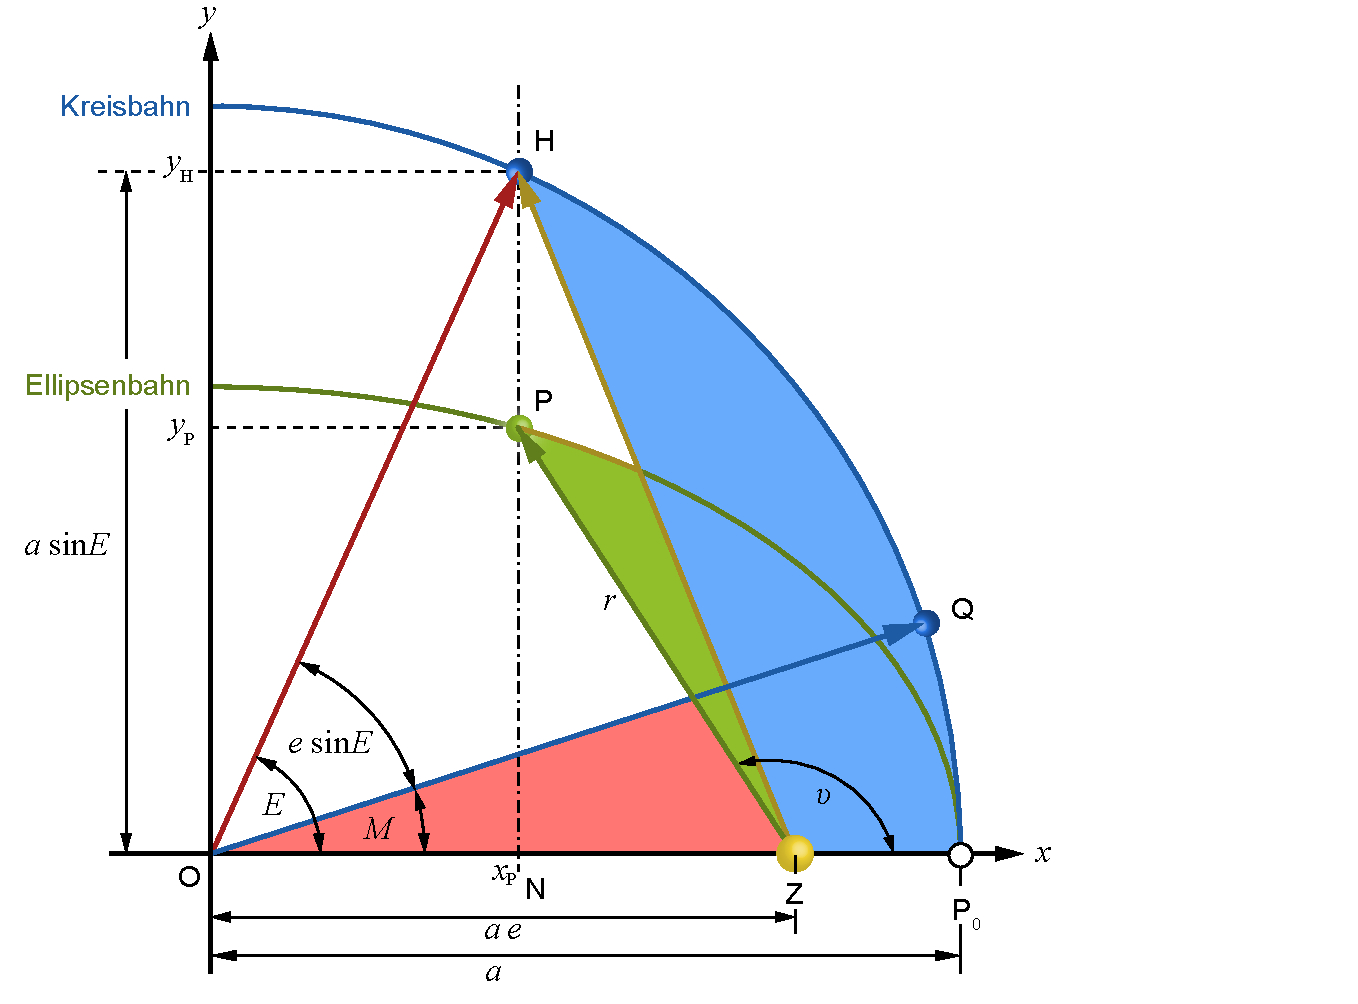
\includegraphics[width=\textwidth]{Geometrie_KG.pdf}
\caption[Geometrische Herleitung der Kepler-Gleichung.]{Geometrische Herleitung der Kepler-Gleichung. Bezeichnungen: P Planet, H "`Hilfsplanet"'"', Q "`Quasiplanet"', $\mathrm{P_0}$ Perihel (siehe Text).}
\label{abb:hm_geom_abl_kepler}
\end{figure}

Wir konstruieren uns einen weiteren Hilfsplaneten H, der dieselbe $x$-Position wie der Planet P hat und dessen $y$-Position sich aber aus der Projektion auf den Kreis mit dem Radius $a$ ergibt.
Den Winkel, der sich aus dem Fahrstrahl vom Kreis/Ellipsenzentrum O zum Hilfsplaneten H relativ zur Apsidenlinie ergibt, bezeichnen wir mit $E$.
Wir wollen zun�chst zeigen, dass der so definierte Winkel $E$ mit der nach \eqref{eq:hm_exzentrische_Anomalie} definierten \textit{exzentrischen Anomalie}\index{Anomalie!exzentrische} $E$ �bereinstimmt.
F�r die $x$-Koordinate $x_\text{P}(t)$ des Punktes $\text{P}(t)$ gilt einerseits
\begin{equation*}
x_\text{P}(t) = a\, e\, + r\,\cos \upsilon
\end{equation*}
und andererseits
\begin{equation*}
x_\text{P}(t) = a\,\cos E \,.
\end{equation*}
Gleichsetzen und Multiplikation mit $e$ ergibt
\begin{equation}
a\,e^2 + r\,e\,\cos \upsilon = a\,e\,\cos E \,. \label{eq:hm_ae_quadrat}
\end{equation}
Wir benutzen die Parameterdarstellung der Ellipse \eqref{eq:hm_bahnglg} in der Form 
	\[r\, e\,\cos \upsilon\!=\! a\,(1-e^2)-r\,,\]
die wir in \eqref{eq:hm_ae_quadrat} einsetzen.
Daraus folgt
\begin{equation}
r = a-a\,e\,\cos E = a\,(1-e\,\cos E) \,. \label{eq:hm_r_param_ellipse} 
\end{equation}
Damit ist die Gleichheit der nach \figref{hm_geom_abl_kepler} geometrisch definierten exzentrischen Anomalie $E$ mit der Definition \eqref{eq:hm_exzentrische_Anomalie} gezeigt.
Jetzt k�nnen wir unter Benutzung des Fl�chensatzes mit rein geometrischen �berlegungen die Kepler-Gleichung aus der Geometrie von \figref{hm_geom_abl_kepler} ableiten.\footnote{Diese Ableitung geht auf Kepler zur�ck und benutzt lediglich den empirisch gefundenen Fl�chensatz, denn 1609 war das Gravitationsgesetz ja noch nicht bekannt!}
Wir betrachten zun�chst die Kreisbogenfl�che $A_{\text{HOP}_0}(t)$.
Sie kann einerseits durch die Kreisbogenfl�che $A_{\text{HOP}_0}(t)\!=\! \pi a^2 E/2\pi \!=\!\lk a^2/2\rk\,E(t)$ (mit $E$ im Bogenma�) und andererseits als Summe der Dreiecksfl�che $A_\text{HOZ}$ und der krummlinigen Dreiecksfl�che $A_{\text{HZP}_0}(t)$ (blau gekennzeichnet) berechnet werden:
\begin{equation*}
A_{\text{HOP}_0}(t) = \frac{a^2}{2} E(t) = \frac{1}{2} a\,e\,a\,\sin E(t)+A_{\text{HZP}_0}(t)  \,.
\end{equation*}
Um eine Bestimmungsgleichung f�r $E(t)$ zu bekommen, m�ssen wir also $A_{\text{HZP}_0}(t)$ berechnen.
Dazu betrachten wir zun�chst die Streckenl�ngen $y_\text{H}\!=\!\overline{\text{NH}}$ und $y_\text{P}\!=\!\overline{\text{NP}}$.
Aus der Kreis- bzw. Ellipsengleichung folgt
\begin{align*}
y_\text{H} &= a \sqrt{1-\frac{\overline{\text{ON}}^2}{a^2}} ~~\text{bzw.} ~~y_\text{P} = b \sqrt{1-\frac{\overline{\text{ON}}^2}{a^2}} \,.
\end{align*}
Daraus folgt, dass sich die Fl�chen $A_\text{PZN}$ und $A_\text{HZN}$ der entsprechenden Dreiecke verhalten wie
\begin{equation}
\frac{A_\text{PZN}}{A_\text{HZN}} = \frac{\frac{1}{2} y_\text{P}\,\overline{\text{ZN}}}{\frac{1}{2} y_\text{H}\,\overline{\text{ZN}}} = \frac{b}{a} \,. \label{eq:hm_A_PZN_durch_A_HZN}
\end{equation}
F�r die Fl�chen der krummlinigen Dreiecke $A_{\text{PNP}_0}$ (Ellipsensegment) und $A_{\text{HNP}_0}$ (Kreissegment) sowie deren Verh�ltnis gilt
\begin{align*}
  A_{\text{PNP}_0} &= \, \int\limits_{a\cos E}^a\!b\sqrt{1-\frac{x^2}{a^2}} \,\D x \; \quad \text{und} \quad
  A_{\text{HNP}_0} = \, \int\limits_{a\cos E}^a\!a\sqrt{1-\frac{x^2}{a^2}} \,\D x \\
  \Rightarrow~~ &~~\frac{A_{\text{PNP}_0}}{A_{\text{HNP}_0}} = \frac{b}{a} \,.
\end{align*}
Da sich sowohl die Dreiecksfl�chen $A_\text{PZN}$ und $A_\text{HZN}$ als auch die krummlinigen Dreiecke $A_{\text{PNP}_0}$ und $A_{\text{HNP}_0}$ jeweils wie $b/a$ verhalten, muss dies auch f�r die Differenzfl�chen $A_{\text{PZP}_0}$ und $A_{\text{HZP}_0}$ gelten.
Damit ist
\begin{equation}
A_{\text{HZP}_0}(t) = \frac{a}{b}\,A_{\text{PZP}_0}(t) \,. \label{eq:hm_r_param_ellipse01} 
\end{equation}
Nun schauen wir uns noch das Verh�ltnis der Fl�che $A_\text{P}(t)\!=\!A_{\text{PZP}_0}$ zur Kreisbogenfl�che $A_\text{Q}(t)\!=\!A_{\text{QOP}_0}$ an.
Nach einem vollen Umlauf $T_\text{P}$ ist $A_\text{P}(T_\text{P})$ die Fl�che der Ellipse $\pi ab$ und $A_\text{Q}(T_\text{P})$ die Fl�che des Kreises $\pi a^2$.
Hier kommt der Fl�chensatz ins Spiel.
Nach diesem muss dieses Verh�ltnis auch f�r jeden beliebigen Zeitpunkt gelten, daher gilt
\begin{equation}
\frac{A_\text{P}(T_\text{P})}{A_\text{Q}(T_\text{P})} = \frac{\pi ab}{\pi a^2} = \frac{A_\text{P}(t)}{A_\text{Q}(t)} = \frac{A_{\text{PZP}_0}}{A_{\text{QOP}_0}} = \frac{b}{a} \,.\label{eq:hm_F_P_durch_F_Q}
\end{equation}
Mit \eqref{eq:hm_r_param_ellipse01} folgt sofort
\begin{equation*}
A_{\text{HZP}_0} = \frac{a}{b} A_{\text{PZP}_0} = \frac{ab}{ba} A_{\text{QOP}_0} = A_{\text{QOP}_0} = \frac{M}{2}a^2 = \frac{a^2}{2}\frac{2\pi}{T_\text{P}}\,(t-t_0) \,.
\end{equation*}
Eingesetzt in die oben gefundene Aufteilung der Fl�che folgt daraus
\begin{equation*}
\frac{a^2}{2}\,E(t) = \frac{1}{2}a\,e\,a\,\sin E(t) + \frac{a^2}{2} M(t)\; ,
\end{equation*}
woraus sich mittels Division durch $a^2/2$ die Kepler-Gleichung ergibt.\\

Wir wollen zum Schluss noch eine n�tzliche Formel f�r $\upsilon(t)$ angeben:
\begin{equation}
\tan \lk \frac{\upsilon}{2} \rk = \sqrt{\frac{1+e}{1-e}}\,\tan\lk\frac{E}{2}\rk\,. \label{eq:hm_nu(t)_alternativ}
\end{equation}
Diese l�sst sich ebenfalls aus der Geometrie der \figref{hm_geom_abl_kepler} herleiten, indem man den Kosinus der wahren Anomalie durch die exzentrische Anomalie ausdr�ckt und die trigonometrische Beziehung f�r den halben Winkel verwendet (\probref{hm_wahre_anomalie}).
�hnliche Bewegungsgleichungen, wie wir sie hier f�r die Ellipse gezeigt haben, k�nnen auch f�r die Parabel und die Hyperbel hergeleitet werden (\probref{hm_bwglg_hyp_parab}).

Jetzt m�ssen wir nur noch die Kepler-Gleichung l�sen. Das hat es aber durchaus in sich.



\section{L�sung der Kepler-Gleichung} \label{kap:lsg_kepler}

Das Besondere an der Kepler-Gleichung ist neben ihrer grundlegenden Bedeutung f�r die Himmelsmechanik ihre offensichtliche Einfachheit und Kompaktheit in der Formulierung (man kann auch sagen Sch�nheit) und ihre gleichzeitige Komplexit�t in der L�sung. Schon Kepler wies darauf hin, dass er f�r die Gleichung keine analytisch geschlossene L�sung finden konnte und stachelte nachfolgende Generationen an, sich der L�sung dieser Aufgabe zu widmen \cite{Kepler1992}.
Neben Newton\indexp{Newton, Sir Isaac}  waren es vor allem Lagrange\footnote{Joseph-Louis Lagrange (1736--1813) war ein italienisch-franz�sischer Mathematiker und Astronom und gilt als Begr�nder der analytischen Mechanik (\emph{M�canique Analytique}, 1788).}\indexp{Lagrange, Joseph-Louis}, Cauchy\footnote{Augustin-Louis Cauchy (1789--1857) war ein franz�sischer Mathematiker, der besonders auf dem Gebiet der Analysis t�tig war.}\indexp{Cauchy, Augustin-Louis} und Bessel\footnote{Friedrich Wilhelm Bessel (1784--1846) war ein deutscher Wissenschaftler, der auf den Gebieten der Astronomie, Mathematik, Geod�sie und Physik bedeutsame Beitr�ge lieferte.}\indexp{Bessel, Friedrich Wilhelm}, die sich dem Thema widmeten und aus der Besch�ftigung mit der Kepler-Gleichung wertvolle und fundamentale Beitr�ge zur Entwicklung der Mathematik lieferten.
Erw�hnt seien die Newton-Raphson-N�herungsmethode, inverse Reihenentwicklungen, komplexe Analysis und die Bessel-Funktionen.
Seither gab es in jeder Dekade mindestens ein oder zwei Arbeiten zur analytisch geschlossenen L�sung der Kepler-Gleichung.
Als aktuelle Beispiele seien die Arbeiten in \cite{Siewert1972} und \cite{Perovich2016} angef�hrt.
Sie reihen sich ein in das Bem�hen, weiter nach einer einfachen analytisch geschlossenen L�sung (zumindest f�r Spezialf�lle) zu suchen.
Wir wollen im Folgenden jedoch die beiden grunds�tzlichen N�herungsmethoden (Iteration und Reihenentwicklung) zur L�sung der Kepler-Gleichung vorstellen.             

\subsection{Iterationsverfahren}\index{Iterationsverfahren} \label{kap:iteration_kepler}
Ein naheliegender Ansatz zur L�sung der Kepler-Gleichung ist die Iteration\index{Iteration}, d.\,h. man berechnet eine N�herung f�r die Gr��e $E_{k+1}(t)$ aus einer zuvor bestimmten N�herung $E_k(t)$ nach
\begin{equation*}
E_{k+1}(t) = M(t) + e\,\sin E_k(t) 
\end{equation*}
mit dem sinnvollerweise zu setzenden \textit{Iterationsanfang}
\begin{equation}
E_0 (t)=M(t) ~.\label{eq:hm_iteration_anfang}
\end{equation}
Das liegt besonders nahe, wenn die Exzentrizit�t $e$ relativ klein ist, weil dann die Abweichung von der Kreisbahn relativ gering ist.
Man kann aber auch andere Iterationsanf�nge w�hlen und in bestimmten F�llen muss man das auch, insbesondere bei gro�en Exzentrizit�ten $e$ \cite{Strebel2001}.
Unter Nutzung der trigonometrischen Additionstheoreme $\sin(x+y)\!=\!\sin x \cos y + \cos x \sin y$ und der N�herung f�r kleine Argumente $\sin x\!\approx\! x -  x^3/6 + \ldots$ bzw. $\cos x\!\approx\! 1-x^2/2 + \ldots$ kann auf \eqref{eq:hm_iteration_anfang} folgend die n�chste Iteration durchgef�hrt werden:\footnote{Wir lassen der Einfachheit halber die Notation der Zeit $t$ weg.}
\begin{equation}
E_1 = M+e\,\sin M ~~. \label{eq:hm_E_1_kepler}
\end{equation}
Der n�chste \textit{Iterationsschritt} lautet:
\begin{align}
\begin{split}
E_2 &= M + e\,\sin E_1 = M + e\,\sin (\underbrace{M+e\,\sin M}_{E_1}) \\
		&= M + e\,\sin M\, \cos(\underbrace{e\,\sin M}_{E_1-E_0})  +  e\,\cos M\, \sin(\underbrace{e\,\sin M}_{E_1-E_0}) \,. 
\end{split} \label{eq:hm_E_2_kepler}
\end{align}
Da $E_{k+1}(t)-E_k(t)\!=\!e\,\sin E_k(t)$ eine kleine Gr��e ist, kann man mit der N�herung f�r kleine Winkel schreiben:
\begin{align*}
E_2 &\approx  M + e\,\sin M\, \lk 1-\frac{e^2}{2} \sin^2 M \rk + e\,\cos M \, e\,\sin M + \mathcal{O}(e^3) \\
    &= M + e\,\sin M + \frac{e^2}{2}\,\sin 2M + \mathcal{O}(e^3) \,. 
\end{align*}
Der n�chste Iterationsschritt ergibt
\begin{equation*}
E_3 \approx M + e\,\sin E_2 = M+e\sin\lk M+e\sin M+\frac{1}{2}e^2 \sin 2M\rk ~~, \label{eq:hm_E_3_kepler}
\end{equation*}
woraus wiederum mit den Additionstheoremen und N�herungen f�r kleine $e$ folgt:
\begin{equation*}
E_3 = M+ \lk e-\frac{1}{8} e^3\rk \sin M + \frac{1}{2}e^2\,\sin 2M + \frac{3}{8}e^3\,\sin 3M + \mathcal{O}(e^4) \,.
\end{equation*}
Verallgemeinert man die Schritte induktiv, erh�lt man
\begin{equation}
E = M+ \sum_{k=1}^{\infty} b_k(e)\,\sin kM \,. \label{eq:hm_reihenentw_iteration}
\end{equation}
Diese Reihe stellt eine Entwicklung nach \anf{Frequenzvielfachen} von $M$ dar.
Das kann auch so verstanden werden, dass die Zeitentwicklung der Bewegung auf der Ellipsenbahn gegen�ber der reinen Kreisbahnbewegung Oberfrequenzen hat, deren Koeffizienten von der Exzentrizit�t $e$ abh�ngen.
Im Fall von $e\!>\!0.6627434$ divergiert die Entwicklung nach \eqref{eq:hm_reihenentw_iteration} \cite{Murray2008}.
Es muss dann auf andere Iterationsverfahren (Regula falsi, Newton-Raphson, Sekanten- und Tangentenverfahren) und andere Iterationsstartwerte zur�ckgegriffen werden \cite{Strebel2001}.
Wir geben hier noch die Entwicklung von \eqref{eq:hm_reihenentw_iteration} bis zur vierten Ordnung von $e$ an:
\begin{align}
\begin{split}
E = M &+\lk e-\frac{1}{8}e^3\rk \sin M + \lk \frac{1}{2} e^2 - \frac{1}{6} e^4 \rk \sin 2M  \\
      &+ \frac{3}{8}e^3\,\sin 3M + \frac{1}{3} e^4\,\sin 4M + \mathcal{O}(e^5) \,. 
\end{split} \label{eq:hm_entwicklung_4Ord}
\end{align}
Damit haben wir eine N�herungsl�sung f�r $E$ gewonnen, aus der man �ber \eqref{eq:hm_nu(t)_alternativ} die wahre Anomalie des Planeten \bzw �ber \eqref{eq:hm_exzentrische_Anomalie} dessen Entfernung zum Zentralk�rper bestimmen kann.
Die L�sung beinhaltet als Parameter lediglich die Exzentrizit�t $e$ und �ber $M$ die gro�e Halbachse $a$ und die Zeitdifferenz zum Anfangswert $t_0$.
Die Frage ist nun, ob die Koeffizienten $b_k(e)$ in \eqref{eq:hm_reihenentw_iteration} in einer allgemeinen Form dargestellt und nicht nur schrittweise �ber ein Iterationsverfahren berechnet werden k�nnen.

\subsection{Reihenentwicklung}\index{Reihenentwicklung}
Da $E\!-\!M\!=\!e\sin E$ f�r kleine $e$ eine kleine Gr��e ist, ist es sinnvoll, die Kepler-Gleichung nach $E\!-\!M$ zu entwickeln.
Wir machen dazu folgenden Ansatz:
\begin{align*}
e\,\sin E &= \sum_{k=1}^{\infty} b_k(e)\,\sin(kM) \Rightarrow b_k(e) = \frac{2}{\pi} \int\limits_0^\pi e\,\sin E\,\sin(kM) \,\D M \,. 
\end{align*}
Mittels partieller Integration unter Nutzung der Kepler-Gleichung ergibt sich
\begin{align*}
b_k(e) &= \underbrace{\frac{2}{k\pi} \lek e\,\sin E\,\cos(kM) \rek^0_\pi}_{=0} + \frac{2}{k\pi} \int\limits_0^\pi \lk \frac{\D E}{\D M} -1\rk \cos(kM)\,\D M \\
       &= \frac{2}{k\pi} \int\limits_0^\pi \cos (kM) \,\D E - \underbrace{\frac{2}{k\pi} \int\limits_0^\pi \cos (kM) \D M}_{=0} \,. 
\end{align*}
Setzen wir $kM =  k\,\lk E - \sin E \rk$ (Kepler-Gleichung) im Integranden, erhalten wir
\begin{equation}
b_k(e) = \frac{2}{k\pi} \int\limits_0^\pi \cos \lek k(E-e\,\sin E)\rek \,\D E \,. \label{eq:hm_b_k(e)}
\end{equation}
Hier verwenden wir jetzt die \emph{Bessel-Funktionen} erster Art $\mathcal{J}_n (z)$, die �ber das \emph{Bessel-Integral} wie folgt definiert \cite{Olver1992} sind:
\begin{align}
  \mathcal{J}_n(z)
  &= \frac{1}{\pi} \int\limits_0^\pi \cos (z\,\sin\theta - n\theta)\,\D \theta 
    = \frac{1}{n!} \lk \frac{z}{2} \rk^n \sum_m^{\infty} (-1)^m \frac{(z/2)^{2m}}
    {m! (n+1)(n+2) \ldots (n+m)} \,.\label{eq:hm_besselfkt_erster_art_int}
\end{align}
Da die cos-Funktion gerade ist, kann \eqref{eq:hm_b_k(e)} mit \eqref{eq:hm_besselfkt_erster_art_int} geschrieben werden als
\begin{equation}
b_k(e) = \frac{2}{k} \mathcal{J}_k(ke) \,. \label{eq:hm_b_k(e)_Bessel}
\end{equation}
Damit l�sst sich die L�sung der Kepler-Gleichung nun als Reihe mit \gls{besselfkt}en schreiben:
\begin{equation}
E = M + 2 \sum_{k=1}^\infty \frac{\mathcal{J}_k(ke)}{k}\,\sin(kM) \,.
\label{eq:hm_lsg_kepler_reihe}
\end{equation}
Wir empfehlen die Reihenentwicklung \eqref{eq:hm_lsg_kepler_reihe} einmal selbst bis zur vierten Ordnung in $e$ durchzuf�hren.
Als Ergebnis erh�lt man eine der Reihe \eqref{eq:hm_entwicklung_4Ord} entsprechenden L�sung.
Numerische Berechnungen zur Konvergenz der Reihe 
\eqref{eq:hm_lsg_kepler_reihe} sind in \probref{hm_bessel} ausgef�hrt.


\subsection{Mittelpunktsgleichung}\label{kap:hm_mpg}
Da \glslink{mittelpunktsglg} bei kleinen Exzentrizit�ten auch die Differenz von wahrer und mittlerer Anomalie eine kleine Gr��e sein sollte, ist f�r viele Problemstellungen eine Reihenentwicklung dieser Differenz direkter und besser geeignet.
Man spart sich dabei den Zwischenschritt der Berechnung von $E$ und die anschlie�ende Umrechnung in $\upsilon$ �ber \eqref{eq:hm_nu(t)_alternativ}.
Eine solche Reihenentwicklung f�r die Differenz von wahrer und mittlerer Anomalie wird auch Mittelpunktsgleichung genannt:
\begin{infobox} {Mittelpunktsgleichung}
\begin{align}
\begin{split}
\mathcal{C}=\upsilon-M &= 2e \sin M + \frac{5}{4}e^2\,\sin(2M) \\
&+ e^3 \lk \frac{13}{12} \sin(3M) - \frac{1}{4} \sin M \rk  \\
&+ e^4 \lk \frac{103}{96} \sin(4M) - \frac{11}{24} \sin(2M)  \rk + \mathcal{O}(e^5) \,. 
\end{split} \label{eq:hm_mpglg_nu-M}
\end{align} \\
\end{infobox}

Da wir die Mittelpunktsgleichung im Folgenden h�ufig brauchen werden, zeigen wir die Herleitung dieser Reihe in Beispiel \ref{bsp:mittelpktglg} und einen alternativen Weg in \probref{hm_alternative_MPG}.
Ebenso kann in �hnlicher Form eine Reihe f�r $r/a$ abgeleitet werden (siehe dazu auch \cite{Brouwer1961,Guthmann2000}):
\begin{align}
\begin{split}
\frac{r}{a} = &1 + \frac{1}{2}e^2 - 2e \sum_k^\infty \frac{1}{k^2} \frac{\D }{\D e} \mathcal{J}_k(ke)\,\cos(kM) \\
            = &1-e \cos M + e^2(1-\cos(2M) + \frac{3}{8}e^3 (\cos M - \cos(3M)  \\
						&+\frac{1}{3} e^4 (\cos(2M) - \cos(4M) + \mathcal{O}(e^5) \,.  
\end{split} \label{eq:hm_mpglg_r/a}
\end{align}

%BEISPIEL 3 %%%%%%%%%%%%%%%%%%%%%%%%%%%%%%%%%%%%%%%%%%%%%%%%%%%%%%%%%%%%%%%%%%%%%%%%%%%%%%%%%%
\begin{example}{Mittelpunktsgleichung}
\textit{Wir wollen die Mittelpunktsgleichung herleiten. Wir starten mit der Beziehung \eqref{eq:hm_drehimpuls_von_ae} f�r den Drehimpuls $r(\upsilon)$ und leiten daraus eine Gleichung f�r $\dot{\upsilon}(r)$ ab, die wir mit $\text{d}M\!=\!2\pi/T_\text{P}\,\text{d}t$ und der Substitution $r$ mittels der Definition der exzentrischen Anomalie in eine Gleichung f�r $\text{d}\upsilon\!=\!f(\text{d}M)$ umformen. Diese Gleichung
enth�lt $\text{d}E/\text{d}M$. F�r $\text{d}E/\text{d}M$ setzen wir die Bessel-Reihe \eqref{eq:hm_lsg_kepler_reihe} ein und k�nnen das Zwischenergebnis dann gliedweise integrieren.}\\

Wir starten also mit der Beziehung f�r den Drehimpuls nach \eqref{eq:hm_drehimpuls_von_ae} und nutzen das 3.~ Keplersche Gesetz:
\begin{align*}
L &= \sqrt{a\mu_\text{G}(1-e^2)} = r^2\,\dot{\upsilon} = \sqrt{1-e^2}\,n_\text{P}\,a^2\,.
\end{align*}
Mit der Definition der exzentrischen Anomalie $r\!=\!a(1-e\cos E)$ k�nnen wir schreiben:
\begin{align}
a^2(1-e\cos E)^2\,\text{d}\upsilon &= n_\text{P}\,a^2\sqrt{1-e^2}\,\text{d}t \nonumber \\
\Rightarrow \text{d}\upsilon &= \frac{\sqrt{1-e^2}}{(1-e\cos E)^2}\,\text{d}M ~~\text{mit}~~ \text{d}t = \frac{1}{n_\text{P}}\,\text{d}M \label{eq:hm_bsp_mpg_9} \,.
\end{align}
Differentiation der Kepler-Gleichung nach $\text{d}M$ ergibt die Beziehung:
\begin{align*}
\frac{\text{d}}{\text{d}M} E &= \frac{\text{d}}{\text{d}M} (M+e\sin E) = 1+e\cos E \frac{\text{d}E}{\text{d}M} ~~\Rightarrow \frac{\text{d}E}{\text{d}M} = \frac{1}{1-e\cos E} \,,
\end{align*}
die wir  in \eqref{eq:hm_bsp_mpg_9} einsetzen und
\begin{equation}
\text{d}\upsilon = \sqrt{1-e^2} \lk \frac{\text{d}E}{\text{d}M} \rk^2 \text{d}M \, \label{eq:hm_bsp_mpg_10}
\end{equation}
erhalten. Das ist schon eine differentielle Form von $\upsilon(M)$, die wir aber noch integrieren m�ssen. 
Um eine integrierbare Form f�r $\text{d}E/\text{d}M$ zu erhalten, leiten wir die Bessel-Reihe \eqref{eq:hm_lsg_kepler_reihe} nach $\text{d}M$ ab:
\begin{align*}
\frac{\text{d}E}{\text{d}M} &= \frac{\text{d}}{\text{d}M} \lk M + 2 \sum_{k=1} \frac{\mathcal{J}_k(ke)}{k}\,\sin(kM) \rk = 1+ 2 \sum_{k=1}\,{\mathcal{J}_k(ke)}\,\cos(kM) \\
                            &= \frac{\text{d}}{\text{d}M} \lk M + e\sin M + \frac{e^2}{2}\sin(2M) + \ldots \rk = 1+e\cos M + e^2\cos(2M) + \mathcal{O}(e^3) ~.
\end{align*}
Hierbei haben wir die Entwicklung der Bessel-Funktion \eqref{eq:hm_besselfkt_erster_art_int} nur bis zum quadratischen Term ber�cksichtigt.
Quadrieren ergibt:
\begin{align*}
\lk\frac{\text{d}E}{\text{d}M}\rk^2 &= [ 1+ \underbrace{e\cos M}_{=x} + \underbrace{e^2\cos(2M)}_{=y} + \:\mathcal{O}(e^3)]^2 \,.
\end{align*} 
Mit der Zwischenrechnung $(1+x+y+\ldots)(1+x+y+\ldots)\!=\!1+2x+2y+2xy+x^2+y^2+\ldots\!=\!1+2x+(2y+x^2)+2xy+\ldots$ erhalten wir zun�chst
\begin{align*}
\lk\frac{\text{d}E}{\text{d}M}\rk^2 &= 1+2e\cos M + 2e^2\cos(2M) + \underbrace{e^2\cos^2 M}_{=\frac{e^2}{2}(1+\cos(2M))} + 2e^3\cos M\cos(2M) \\
&= 1+2e\cos M + \frac{1}{2}e^2 + \frac{5}{2} e^2\cos(2M) + 2e^3\cos M\cos(2M)
\end{align*}
und damit �ber Integration von \eqref{eq:hm_bsp_mpg_10} schlie�lich
\begin{align}
\begin{split}
\upsilon &= \lk M + 2e\sin M + \frac{5}{4} e^2\sin(2M) + \frac{1}{2} e^2 M \rk \lk 1-\frac{1}{2} e^2+\ldots \rk \\ 
\upsilon &= M + 2e\sin M + \frac{5}{4}e^2\sin(2M) + \mathcal{O}(e^3) \,. 
\end{split}\label{eq:hm_bsp_mpg_12}
\end{align}
Wir empfehlen in den \textbf{�bungen} \ref{prob:hm_iteration} und \ref{prob:hm_bessel} die Entwicklung  von \eqref{eq:hm_bsp_mpg_12} bis zu Ordnungen $\mathcal{O}(\geq e^4)$ auszuf�hren.
Man kann dazu auch die Symbolic Math Toolbox von \matlab{} oder �hnliche Tools nutzen.\\

\label{bsp:mittelpktglg}
\end{example}
%BEISPIEL %%%%%%%%%%%%%%%%%%%%%%%%%%%%%%%%%%%%%%%%%%%%%%%%%%%%%%%%%%%%%%%%%%%%%%%%%%%%%%%%%%

Mit der nun vorliegenden L�sung der Kepler-Gleichung wollen wir uns erst einmal auf das System Sonne-Erde konzentrieren, um anschlie�end auch Bahnen von Planeten und Kometen zu berechnen.





\section{Himmelsmechanik unseres Sonnensystems}\label{kap:hm_keplergleichung}

\subsection{Erdbahn (Ekliptik)}\index{Erdbahn} \label{kap:erdbahn}
Wegen der besonderen Bedeutung der Erdbahn (Ekliptik) \glslink{ekliptik} bzw. der scheinbaren \anf{Sonnenbahn}\index{Sonnenbahn!scheinbare} (im geozentrischen System) f�r viele Himmelsph�nomene wollen wir uns mit der Erdbahn etwas n�her besch�ftigen.
Sie wird in guter N�herung durch eine Keplerellipse beschrieben, deren geringe numerische Exzentrizit�t $e\!\approx\!0.0167$ die Bahn nur relativ wenig von einer Kreisbahn abweichen l�sst.
Einige Bahnparameter hatten wir bereits eingef�hrt (Tabelle \ref{tab:hm_bahnparameter}).
Die gro�e Halbachse $a = a_\text{\earth}$ der Erdbahn betr�gt etwa 149.6 Millionen Kilometer, woraus sich �ber den mittleren Abstand der Erde von der Sonne die \gls{ae} AE ergibt.
Im zeitlichen Mittel betr�gt der Abstand zwischen Erde und Sonne etwas mehr als eine AE (n�mlich $1.00014\:\text{AE}$), da sich die Erde wegen ihrer ungleichf�rmigen Bahngeschwindigkeit etwas l�nger in Sonnenferne aufh�lt als in Sonnenn�he (\probref{hm_erdbahn_im_jahr}). 

Wir m�ssen an dieser Stelle noch eine Bemerkung zum Abstand zwischen Sonne (\astrosun) und Erde (\earth) machen: Wegen der gro�en Massenverh�ltnisse $m_\text{\astrosun} \gg m_\text{\earth}$ ist das ZKP effektiv ein Eink�rperproblem, \dh in guter N�herung bewegt sich die Erde um die \anf{ruhende} Sonne.
Nun hat die Erde ja aber einen durchaus massereichen Mond (\leftmoon).
Daher bewegt sich nicht der Erdmittelpunkt auf der Kepler-Ellipse um die Sonne, sondern der gemeinsame Schwerpunkt von Mond und Erde.
Dieser Schwerpunkt liegt im Erdinneren \ca $\SI{4000}{\kilo\metre}$ vom Erdmittelpunkt entfernt.
Der Erdmittelpunkt selbst kreist um diesen Schwerpunkt und vollf�hrt folglich eine Art Schlangenlinie entlang der Ellipsenbahn mit einer Periode entsprechend der Umlaufzeit des Mondes um die Erde.
Wenn wir im Folgenden von der \anf{Erdbahn} sprechen, ist in der Regel die gleichm��ige Ellipsenbahn des Erde-Mond-Schwerpunkts gemeint.
Bei Angabe von Zeitpunkten, in denen bestimmte Bahnpunkte durchlaufen werden (\zb das Perihel), ist daher zu unterscheiden, ob sich die Angaben auf den Erde-Mond-Schwerpunkt oder auf den Erdmittelpunkt beziehen (siehe auch Tabelle \ref{tab:hm_bahnparameter} im Tabellenanhang).

F�r die Berechnung der Bahn als Funktion der Zeit messen wir die Zeit in Bruchteilen von Julianischen Jahrhunderten, die seit dem Zeitpunkt J\,2000 $=$ 01.\,01.\,2000, 12:00 UT $=$ 2451545.0 vergangen sind.
Wir benutzen dann anstelle von $T$ (in Julianischen Tagen) zur besseren Unterscheidung die Bezeichnung $t$ f�r (vergangene) Julianische Jahrhunderte:
\begin{equation}
t = \frac{T-\text{J\,2000}}{36525} = \frac{T- 2451545.0}{36525} = \frac{\text{MJD}-51544.5}{36525}~.\\
\label{eq:hm_julian_centuries}
\end{equation}

\begin{figure}%
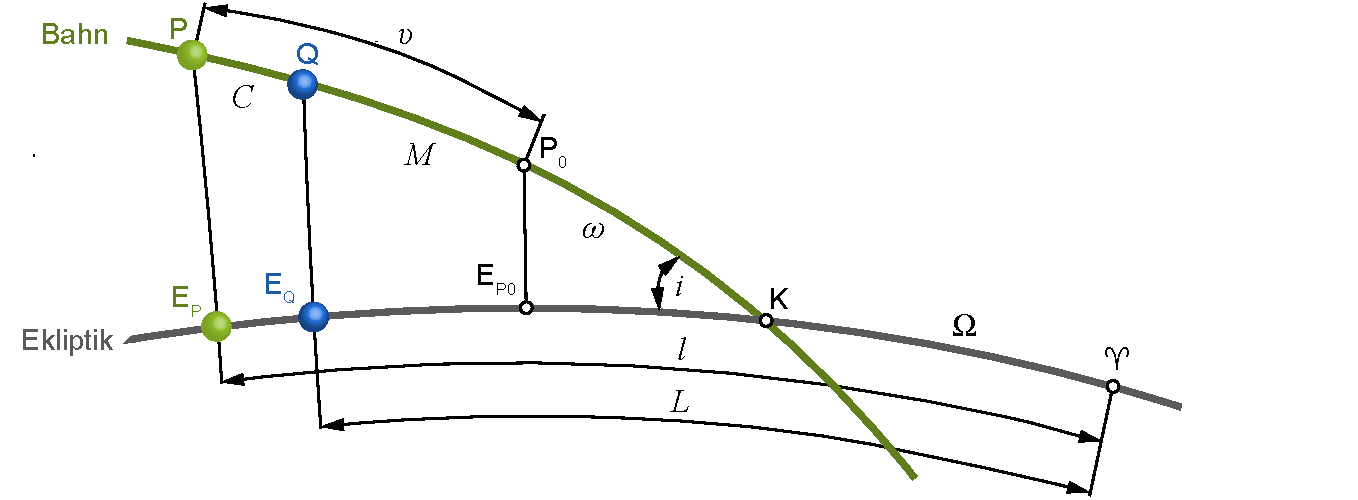
\includegraphics[width=\textwidth]{Bahn_Ekliptik.pdf}%
\caption[Verlauf einer Planetenbahn relativ zur Ekliptik.]{Verlauf einer Planetenbahn relativ zur Ekliptik. Gezeigt ist die Bahn eines Planeten P in der N�he des Fr�hlingspunktes $\vernal$ und des aufsteigenden Knotens K. Dieser ist bei der Erdbahn nicht definiert. Deswegen wird der Fr�hlingspunkt $\vernal$ als Bezugspunkt der Bahngleichung genommen (mathematisch gleichbedeutend mit $\Omega=0$). $\text{P}_0$ bezeichnet das Perihel, $\text{E}_\text{P}$ die Projektion des Planeten P auf die Ekliptik und $\text{E}_\text{Q}$  die Projektion des Hilfsplaneten Q. Dieser entspricht quasi einem auf der Kreisbahn mit der entsprechenden mittleren Anomalie $M$ sich mit konstanter Geschwindigkeit bewegenden \anf{mittleren} Planeten.}
\label{abb:hm_planetenbahnen_rel_ekliptik}
\end{figure}

Um die Position der Erde relativ zur Sonne \bzw sp�ter eines beliebigen Planeten als Funktion der Zeit zu berechnen, betrachten wir \figref{hm_planetenbahnen_rel_ekliptik}.
Wir schauen quasi von der Sonne in der Ekliptik-Ebene auf die Bahn des Planeten in Richtung des aufsteigenden Knotens\glslink{aufstknoten}\ K,
und haben auch den Fr�hlingspunkt $\vernal$ ins Blickfeld gelegt.\footnote{Die Abbildung entspricht der Darstellung \ref{abb:hm_bahnelemente}, aber aus einer anderen Perspektive.}\\
F�r die Erde vereinfacht sich das Bild erheblich, da $i\!=\!0$ und $\Omega\!=\!0$ (�quinoktium des Datums).
Wir k�nnen zun�chst relativ einfache Formeln f�r die heliozentrisch-ekliptikale L�nge der Erde $l_\text{\earth}$ (siehe \ref{tab:hm_astro_KOS}) gewinnen: 
\begin{align} 
\begin{split}
l_\text{\earth} &= \upsilon + \omega + \Omega\ = \upsilon + \varpi = (\upsilon-M)+M+\varpi \\
                &= \mathcal{C} + M + \varpi \,, 
\end{split} \label{eq:hm_ekl_laenge_erde1}
\end{align}
worin $\mathcal{C}\!=\!\upsilon-M$ die \gls{mittelpunktsglg} \eqref{eq:hm_mpglg_nu-M} ist.
F�r die heliozentrische Breite der Erde gilt $b_\text{\earth}\!=\!0$.
Wir wollen die Zeitabh�ngigkeit explizit ausdr�cken und w�hlen als Zeitreferenzpunkt die Epoche $t_\text{E}$ (\zb J2000).
\begin{align} 
l_\text{\earth} &= \mathcal{C}(t-t_\text{E}) + M(t-t_\text{E}) + \varpi_0 + \dot\varpi (t-t_\text{E}) \,, \label{eq:hm_ekl_laenge_erde2}
\end{align}
worin $\varpi_0 = \varpi(t_\text{E})$ ist und wir den linearen Term in der zeitlichen Entwicklung von $\varpi$ explizit mitgenommen haben (entsprechend Tabelle \ref{tab:hm_zeitl_aenderung_bahnparameter_lin}).
Dieser Term repr�sentiert die bereits erw�hnte Verschiebung des Fr�hlingspunktes durch die Pr�zession der Erdachse.
Wir schreiben die mittlere Anomalie $M(t)$ nach \eqref{eq:hm_mittlere_anomalie} als:
\begin{equation}
M(t-t_\text{E}) = n_\text{anom} \cdot (t-t_\text{E}) = n_\text{anom}\,t + M_0 \\
\label{eq:hm_mittlere_anomalie_ansatz}
\end{equation}
mit $M_0\!=\!357.5256\degree$ und $n_\text{anom}\!=\! 360\degree \cdot 36525/T_\text{anom}\!=\!35999.0498\,\degree/\text{Jh.}$ (\cite{Meeus1998,Montenbruck2001,Montenbruck1999} und Tabelle \ref{tab:hm_bahnparameter}).
Hierin ist $T_\text{anom}\!=\!365.259636\: \text{d}$ das \glslink{anomjahr}{anomalistische Jahr}\index{Jahr!anomalistisches}, also die Zeit zwischen zwei Durchg�ngen der Erde durch das Perihel.\\
Andererseits ist die \emph{mittlere L�nge} $L_\text{\earth}(t)$ der Erde definiert als die ekliptikale L�nge einer mit konstanter Umlaufgeschwindigkeit $n_\text{trop}$ (gegeben durch die Umlaufzeit eines tropischen Jahres) auf einer Kreisbahn umlaufenden \emph{mittleren Erde} (siehe Definition des tropischen Jahres in \kapitel{hm_zeitdefinition}), also
\begin{equation}
L_\text{\earth}(t) = n_\text{trop}\,t + L_\text{\earth0} ~ .\\ \label{eq:hm_ekl_laenge_erde3}
\end{equation}
Hier ist $L_\text{\earth0}$ die mittlere L�nge zum Zeitpunkt $t_\text{E}$ (also zur Epoche) und \linebreak $n_\text{trop}\!=\! 360\degree \cdot 36525 / T_\text{trop}\!=\! 36000.7690\:\degree/\text{Jh}$.
Die Differenz von Gleichung \eqref{eq:hm_ekl_laenge_erde3} und \eqref{eq:hm_ekl_laenge_erde2} ergibt dann (f�r die mittlere L�nge ist $\mathcal{C} = 0$)
\begin{align}
M(t) - L_\text{\earth}(t) = \varpi(t) = \dot \varpi \, t + \varpi_0 = (n_\text{anom} -n_\text{trop})\cdot t + (M_0-L_\text{\earth0}) ~,\label{eq:hm_ekl_laenge_erde4}
\end{align}
worin $\varpi_0\!=\! 102.9400\degree$ die L�nge des Perihels zur Epoche $t_\text{E}$ ist.
Der Term $ (n_\text{anom} -n_\text{trop})\, t $ beschreibt die Verschiebung des Fr�hlingspunktes auf Grund der Pr�zession.\\
Wir k�nnen also zusammenfassen: Die wahre ekliptikale L�nge\index{L�nge!ekliptikale}\index{Koordinaten!ekliptikale} $l_\text{\earth}$ des Planeten berechnet sich aus der Summe der Mittelpunktsgleichung $\mathcal{C}$ (hier wird jetzt auch der Begriff \anf{Anomalie} sinnf�llig), der mittleren Anomalie $M$ und der (zeitabh�ngigen) L�nge des Perihels $\varpi$.\footnote{Wir weisen nochmals darauf hin, dass $\varpi\!=\!\omega + \Omega$ kein echter Winkel ist, sondern die Summe aus zwei Winkeln in verschiedenen Ebenen darstellt.}
Wir werden die Gleichungen \eqref{eq:hm_ekl_laenge_erde1} \eqref{eq:hm_ekl_laenge_erde2} in den folgenden Kapiteln ausgiebig verwenden und geben sie deshalb hier auch mit numerischen Werten im Gradma� ($l_\text{\earth}\degree)$ bis zur Ordnung $e^3$ an:
\begin{align} 
l_\text{\earth} =& (2e - \frac{e^3}{4})\,\sin M + \frac{5}{4} e^2 \,\sin(2M) + e^3 \lk \frac{13}{12}\sin(3M) - \frac{1}{4} \sin M \rk + M + \varpi ~,\label{eq:hm_ekl_laenge_bogenmass}
\end{align}
\begin{align}
\begin{split} 
l_\text{\earth}\degree(t) =& \underbrace{1.914443\degree\,\sin M + 0.019996\degree\,\sin(2M) + 0.0002895\degree\,\sin(3M)}_{=\mathcal{C}(M(t))} \\ 
                    &+ \underbrace{35999.0498\:\frac{\degree}{\text{Jh.}}\: t + 357.5256\degree}_{=M(t)} + \underbrace{102.9400\degree + 1.7192\:\frac{\degree}{\text{Jh.}}\:t}_{=\varpi(t)} ~. \nonumber
\end{split} \label{eq:hm_ekl_laenge_gradmass}
\end{align}
$r_\text{\earth}(t)$ berechnet sich direkt aus \eqref{eq:hm_mpglg_r/a} durch Multiplikation mit $a$. \\
Wir k�nnen nun ins geozentrische Bild wechseln und aus den Erdkoordinaten sehr einfach die geozentrisch-ekliptikale L�nge $\lambda_\text{\astrosun}$ der Sonne berechnen.
Da sich an der Zeitdynamik und den relativen Abst�nden nichts �ndert, ist dies geometrisch gesehen einfach ein Wechsel des Bezugspunktes: 
\begin{equation} 
\lambda_\text{\astrosun}(t) = l_\text{\earth}(t) + 180\degree ~\ \textrm{und} ~\ \beta_\text{\astrosun}(t) = -\beta_\text{\earth}(t) \approx\,0 \,. \\
\label{eq:hm_lambda_S(T)}
\end{equation}

Mit den Beziehungen \eqref{eq:hm_ekl_laenge_bogenmass}--\eqref{eq:hm_lambda_S(T)} haben wir nun ein gutes Instrumentarium zur Verf�gung, um f�r jeden Zeitpunkt aus $\lambda_\text{\astrosun}(t)$ die Koordinaten $(\alpha_\text{\astrosun},\,\delta_\text{\astrosun})$ �ber die Transformation aus dem ekliptikalen ins �quatoriale KOS der Sonne nach \eqref{eq:hm_drehung_x_achse_linear2} zu berechnen. 

\subsection{Berechnung der Kulmination der Sonne (Analemma) und ihrer Auf- und Unterg�nge} \label{kap:kulmination_sonne}

Die t�gliche und j�hrliche \anf{Bewegung} der Sonne aus Sicht eines geozentrischen (\bzw topozentrischen) Beobachters auf der Erde z�hlt mit Sicherheit zu den fr�hesten physikalisch-astronomischen Beobachtungen und Messungen der Menschheit.
Die Beobachtungen von Auf- und Unterg�ngen der Sonne, ihres H�chststandes (\textit{Kulmination}) \glslink{kulmination} und den jeweiligen jahreszeitlichen Ver�nderungen \glslink{analemma} waren Grundlage der astronomischen Weltbilder seit den ersten Zivilisationen und ebenso bestimmend f�r Zeitmessung und Navigation.
Es ist daher kein Wunder, dass gerade die hochentwickelten Kulturen der Menschheitsgeschichte besonders ausgefeilte und genaue Kalender und andere Zeitmesssysteme auf Basis von Sonnen- und Mondlauf hatten und diese �ber Jahrhunderte bis zur Entwicklung von Uhren mit hoher Pr�zision Grundlage der menschlichen Zeitmessung waren (siehe \kapitel{hm_zeitdefinition}).

Wir wollen in diesem Kapitel Aufgangs- und Untergangszeiten der Sonne, sowie den Zeitpunkt ihrer Kulmination f�r verschiedene geographische Breiten und L�ngen auf der Erdoberfl�che\index{L�ngengrad}\index{Breitengrad} und jeden Tag des Jahres berechnen.
Wir werden dabei mit der L�sung der Kepler-Gleichung die Bewegung der Erde um die Sonne beschreiben und zeigen, dass damit die verschiedenen Ph�nomene gut berechenbar sind.
Anschlie�end wollen wir einfache Praxisformeln herleiten. 

Wir werden in den folgenden Kapiteln h�ufig von der (scheinbaren) Bewegung der Sonne um die Erde sprechen.
Selbstverst�ndlich meinen wir damit eigentlich die Bewegung der Erde um die Sonne.
Die scheinbare und wahre Bewegung sind �ber die in Tabelle \ref{tab:hm_Umrechung_KOS} im Tabellenanhang angegebene Transformation vom heliozentrischen ins geozentrische KOS (siehe \kapitel{hm_koordinatensysteme}) einfach ineinander �berf�hrbar.
Oft ist das geozentrische Bild mit der (scheinbaren) Bewegung der Sonne sogar anschaulicher und wird deswegen auch gern benutzt.

\subsubsection{Die Zeitgleichung und das Analemma} \label{kap:zeitgleichung}

Wir wissen bereits, dass die Kulmination der wahren Sonne von der Kulmination der mittleren Sonne (die laut Definition genau um 12:00 MOZ kulminiert) abweichen wird.
Die mittlere Sonne \anf{bewegt} sich gleichm��ig entlang des �quators.
Die wahre Sonne hat entlang ihrer elliptischen Bahn unterschiedliche Geschwindigkeiten (2.\ Keplersches Gesetz) und au�erdem erfolgt ihre scheinbare Bewegung entlang der Ekliptik, die ja gegen den �quator geneigt ist.
Beide Sonnen \anf{treffen} aber definitionsgem�� nach dem Ablauf eines Jahres wieder zusammen, haben also die gleiche Umlaufzeit.
Das Vorgehen bei der Berechnung der Kulmination ist nun wie folgt: 
\begin{itemize}
	\item Aus der L�sung der Kepler-Geichung\index{Kepler-Gleichung} berechnen wir im heliozentrischen Koordinatensystem die heliozentrisch-ekliptikale L�nge der Erde \eqref{eq:hm_ekl_laenge_bogenmass} als Funktion der Zeit (\zb jeweils am Mittag 12:00 UT an den jeweiligen Tagen eines Jahres).\footnote{Streng genommen m�ssten wir f�r diese Berechnung die ET anstelle UT nehmen. F�r unsere Rechnung kann man das aber vernachl�ssigen. Warum? �berpr�fen Sie die Abweichung.}
          Wir benutzen daf�r die Bezeichnung $t_\text{d}$.
	\item Daraus ermitteln wir die geozentrisch-ekliptikale L�nge der Sonne $\lambda_\text{\astrosun}(t_\text{d}$) und rechnen diese in geozentrisch-�quatoriale Koordinaten $\alpha_\text{\astrosun}(t_\text{d}), \delta_\text{\astrosun}(t_\text{d})$ um:
\begin{align} 
\begin{split}
	\alpha_\text{\astrosun}(t_\text{d}) &= \arctan\lek \cos\epsilon\tan\lambda_\text{\astrosun}(t_\text{d})\rek \,, \\
	\delta_\text{\astrosun}(t_\text{d}) &= \arcsin\lek\sin\epsilon\sin\lambda_\text{\astrosun}(t_\text{d})\rek \,.
\end{split} \label{eq:hm_alpha_s_delta_s}
\end{align}
\item Wir erhalten so die Deklination und die Rektaszension der (wahren) Sonne als Funktion der Zeit.
\item Wir berechnen dann die Sternzeit nach \eqref{eq:hm_UT_2} und erhalten daraus �ber \eqref{eq:hm_std_winkel_tau} den Stundenwinkel $\tau_\text{ZGL}$ der Sonne.
  Dieser entspricht der sogenannten \emph{\gls{zeitglg}} (ZGL).
  Der Stundenwinkel ist ja f�r ein Himmelsobjekt laut \kapitel{hm_zeitdefinition} die Zeit, die ein K�rper noch bis zum Meridiandurchgang braucht oder bereits hinter sich hat.
  Damit gibt die Zeitgleichung das Vor- bzw. Nachgehen der (wahren) Sonne gegen�ber einer gleichm��ig laufenden mittleren Sonne (UT) an:
\begin{equation} \label{eq:hm_tau_zgl}
\tau_\text{ZGL}= \text{WOZ}-\MOZ=\tau_\text{w,\astrosun}=\theta_\text{w}(t_\text{d})\!-\!\alpha_\text{\astrosun}(t_\text{d}) \,.
\end{equation}
\end{itemize}
\begin{figure}
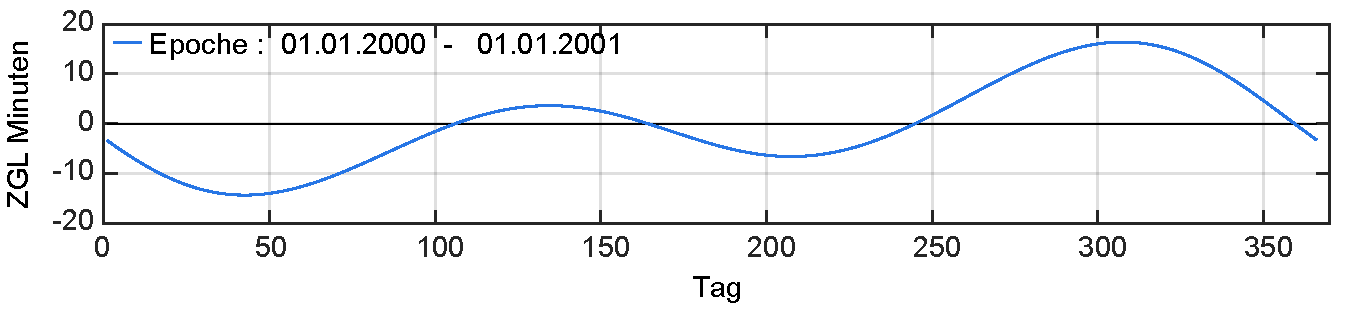
\includegraphics[width=\textwidth]{ZGL01a.pdf}\\
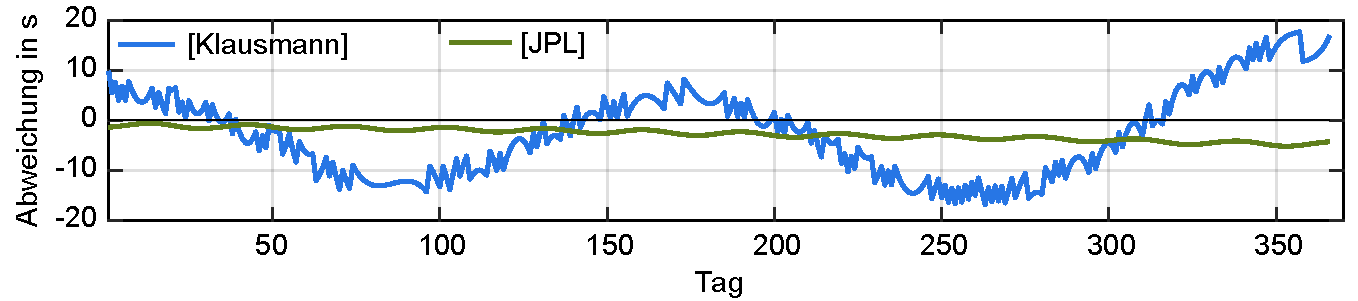
\includegraphics[width=\textwidth]{ZGL01b.pdf}\\
\caption[Berechnete Zeitgleichung und Abweichung von publizierten Werten.]{Berechnete Zeitgleichung und Abweichung von publizierten Werten nach Klausmann \cite{Klausmann1990} und JPL \cite{JPL2020}.}
\label{abb:hm_Zeitgleichung}
\end{figure}
Mit der Zeitgleichung \eqref{eq:hm_tau_zgl}, die in \figref{hm_Zeitgleichung} aufgetragen ist, k�nnen wir somit direkt die t�gliche Abweichung der Kulminationszeit der (wahren) Sonne von 12:00 lokaler (mittlerer) Ortszeit berechnen.
Wir erkennen, dass von Jahresbeginn bis ins Fr�hjahr die wahre Sonne der mittleren Sonne voraus ist.
Die Verh�ltnisse kehren sich dann im Sommer um.
Im Herbst und fr�hen Winter hinkt die wahre Sonne dann der mittleren hinterher. \\
Mit \eqref{eq:hm_UT_3} l�sst sich die Kulminationszeit f�r jede geographische L�nge einfach berechnen.
\figref{hm_Zeitgleichung} zeigt die Abweichung unserer Rechnung von hochgenauen Rechnungen wie sie vom JPL \cite{JPL2020} zur Verf�gung gestellt werden.
Die �bereinstimmung ist sehr gut.%
\footnote{In der Abbildung wird sichtbar, dass in der JPL-Rechnung St�rungen der reinen Keplerbahn durch den Mond zu einer periodischen Abweichung in Monatsabst�nden und zu einer Abweichung auf einer gr��eren Zeitskala f�hren.}
Beim Vergleich mit den empirischen Daten aus \cite{Klausmann1990} muss man ber�cksichtigen, dass diese �ber viele Jahre gemittelt wurden, sodass hier neben dem Schaltjahreseffekt\index{Schaltjahr} (366 anstelle von 365 Tagen) auch j�hrliche Ver�nderungen der Bahnparameter und insbesondere des Fr�hlingspunktes eingehen.

Tr�gt man f�r die Sonne deren Deklination �ber ihren Stundenwinkel (f�r \zb 12:00 UT) f�r jeden Tag des Jahres auf, dann erh�lt man ein sogenanntes \emph{Analemma}\index{Analemma}\glslink{analemma}.
In \figref{hm_Analemma_01} zeigen wir Analemmas f�r jeweils drei verschiedene Exzentrizit�ten $e$ und Ekliptikschiefen $\epsilon$.
W�re die Erdbahn kreisf�rmig und die Erdachse normal zur Ekliptik, dann w�re die Zeitgleichung konstant gleich $0$.
Die Abh�ngigkeit des Analemmas von Exzentrizit�t $e$ und Ekliptikschiefe $\epsilon$ kann man zur Bestimmung dieser Parameter aus dem Analemma nutzen (\mscr e \mlhmref{AnalemmaOkoFit.m} und \mlhmref{AnalemmaFindExz.m}). 

\begin{figure}
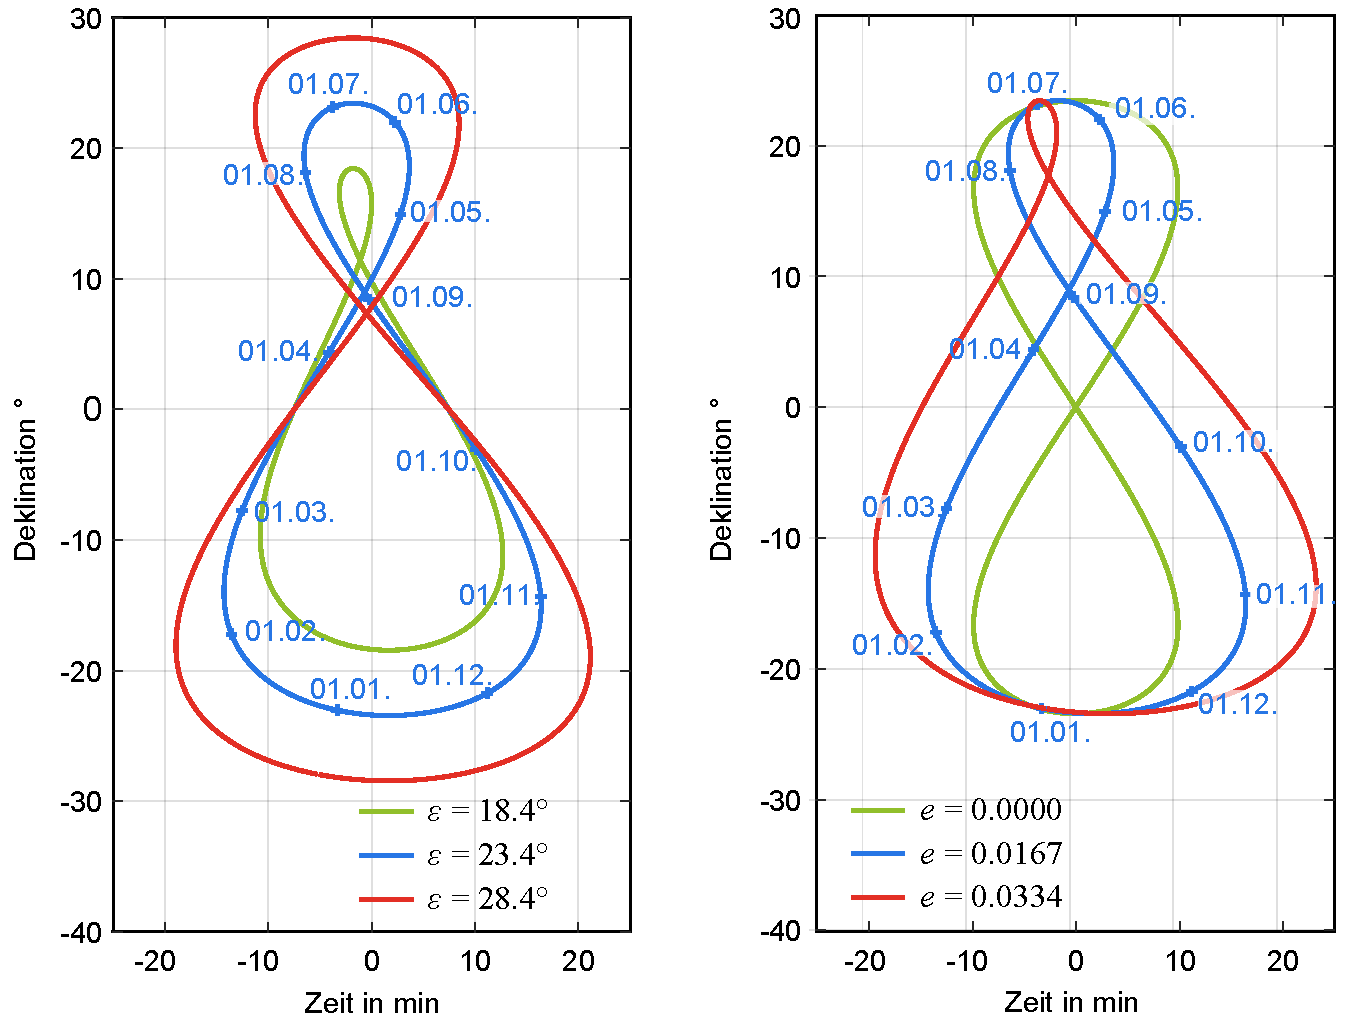
\includegraphics[width=\textwidth]{Analemma01.pdf}
\caption[Berechnete Analemmas f�r verschiedene Parameter.]{Berechnete Analemmas f�r verschiedene Parameter $\epsilon$, $e$ (vgl. \mscr{} \mlhmref{Analemma01.m}).}
\label{abb:hm_Analemma_01}
\end{figure}

Zur Beobachtung eines Analemmas nimmt man im Laufe eines Jahres an jedem Tag zum gleichen Zeitpunkt (auf $\pm 2\:\text{s}$ genau) mit einer fest montierten Kamera (Sonnenbeobachtungs-Schutzfilter nicht vergessen!) ein Bild auf und �berlagert am Ende eines Jahres alle Aufnahmen mit einem Hintergrundbild.%
In \figref{hm_Analemma_02} zeigen wir ein Analemma, welches in den Jahren 2019/20 t�glich um 08:40 MOZ aufgenommen wurde und dessen Fit an die berechnete Kurve (\mscr{} \mlhmref{AnalemmaOkoFit.m}).\footnote{Das Komposit wurde von Bertram H�nlinger, Dietmar Mondon und Michael Kaschke mit einer Nikon D800 und einem ZEISS Classic Distagon T$\ast$ 2.8/21 ZF.2 Objektiv aufgenommen. Man bekommt so �brigens auch einen nachtr�glichen Wetterbericht �ber die Anzahl der Sonnentage.} 
Um einen Fit mit den berechneten Kurven zu bekommen, �berf�hrt man sowohl die Aufnahmedaten als auch die Vorw�rtsberechnungen in das topozentrisch-horizontale KOS, wobei es dabei zu den charakteristischen Verzeichnungen kommt.
Man erkennt sehr gut, dass die Annahme einer doppelt so gro�en Exzentrizit�t der Erdbahn zu einer massiven Abweichung des berechneten Analemmas von der beobachten Kurve f�hren w�rde.
F�r die Bilddatenumrechnung sei an dieser Stelle auf die detaillierte Darstellung in \cite{Montenbruck2001} und \cite{Smart1986} verwiesen. 

\begin{figure}
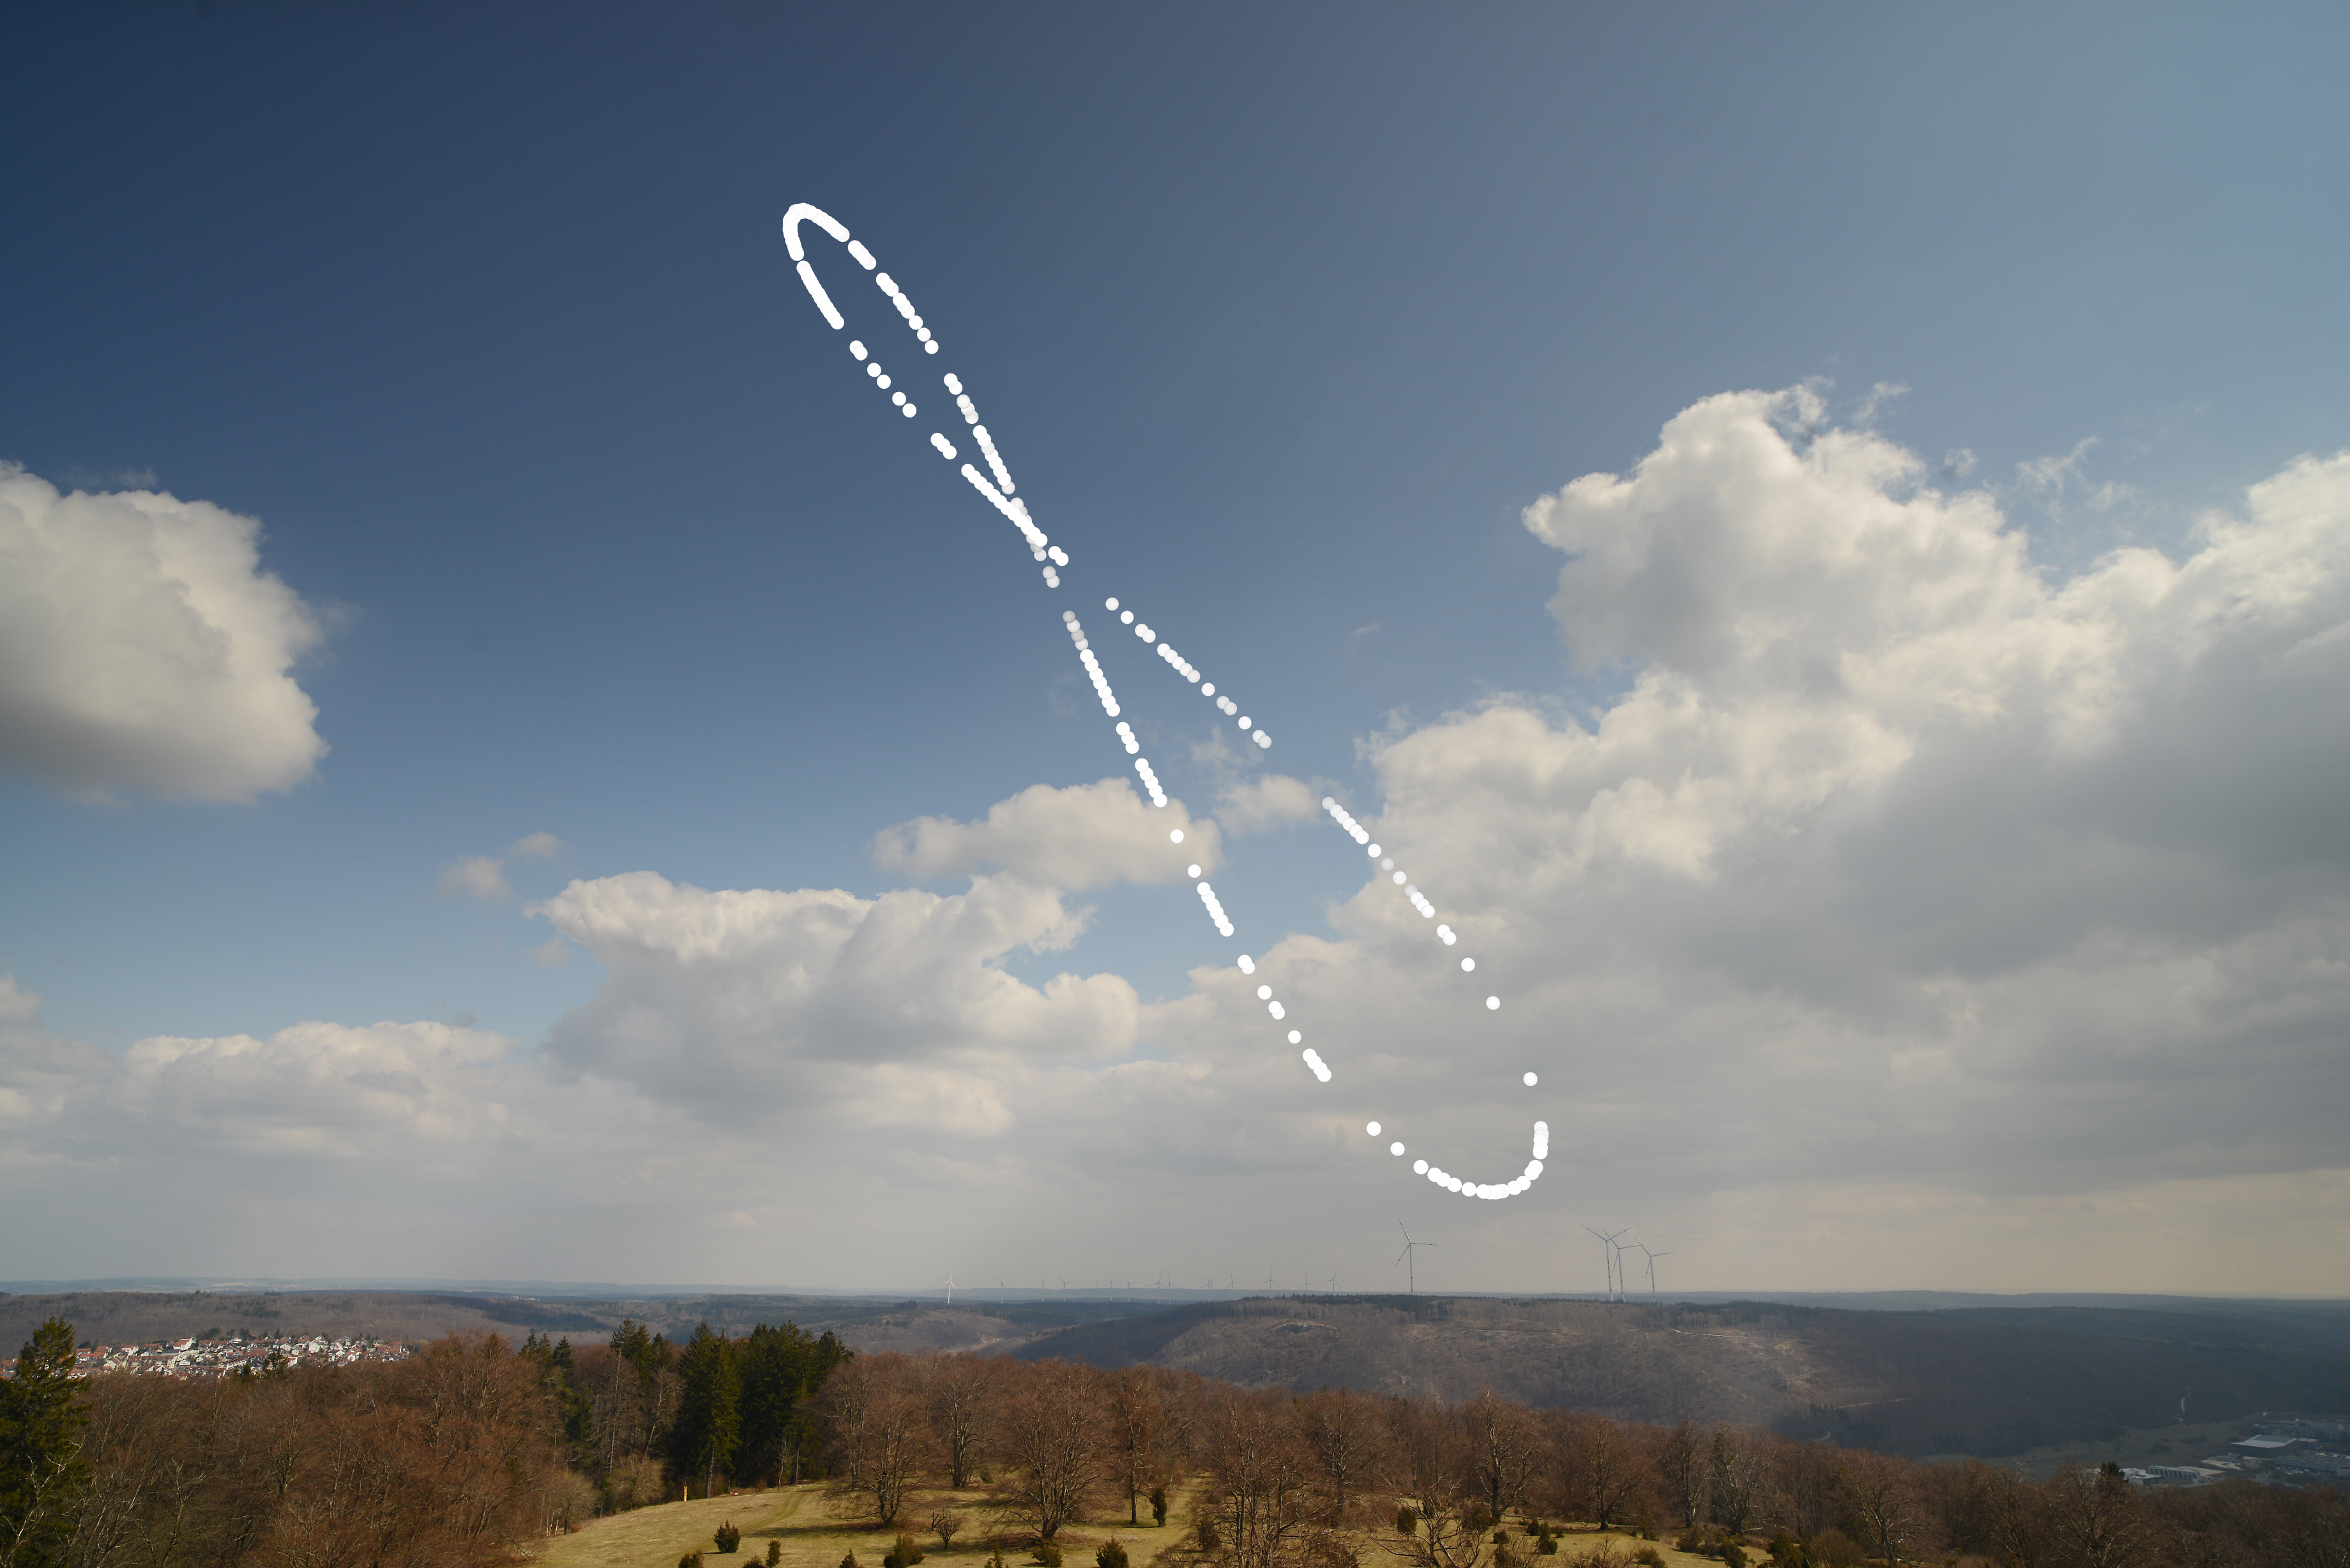
\includegraphics[width=1.0\textwidth]{Analemma2020.jpg}
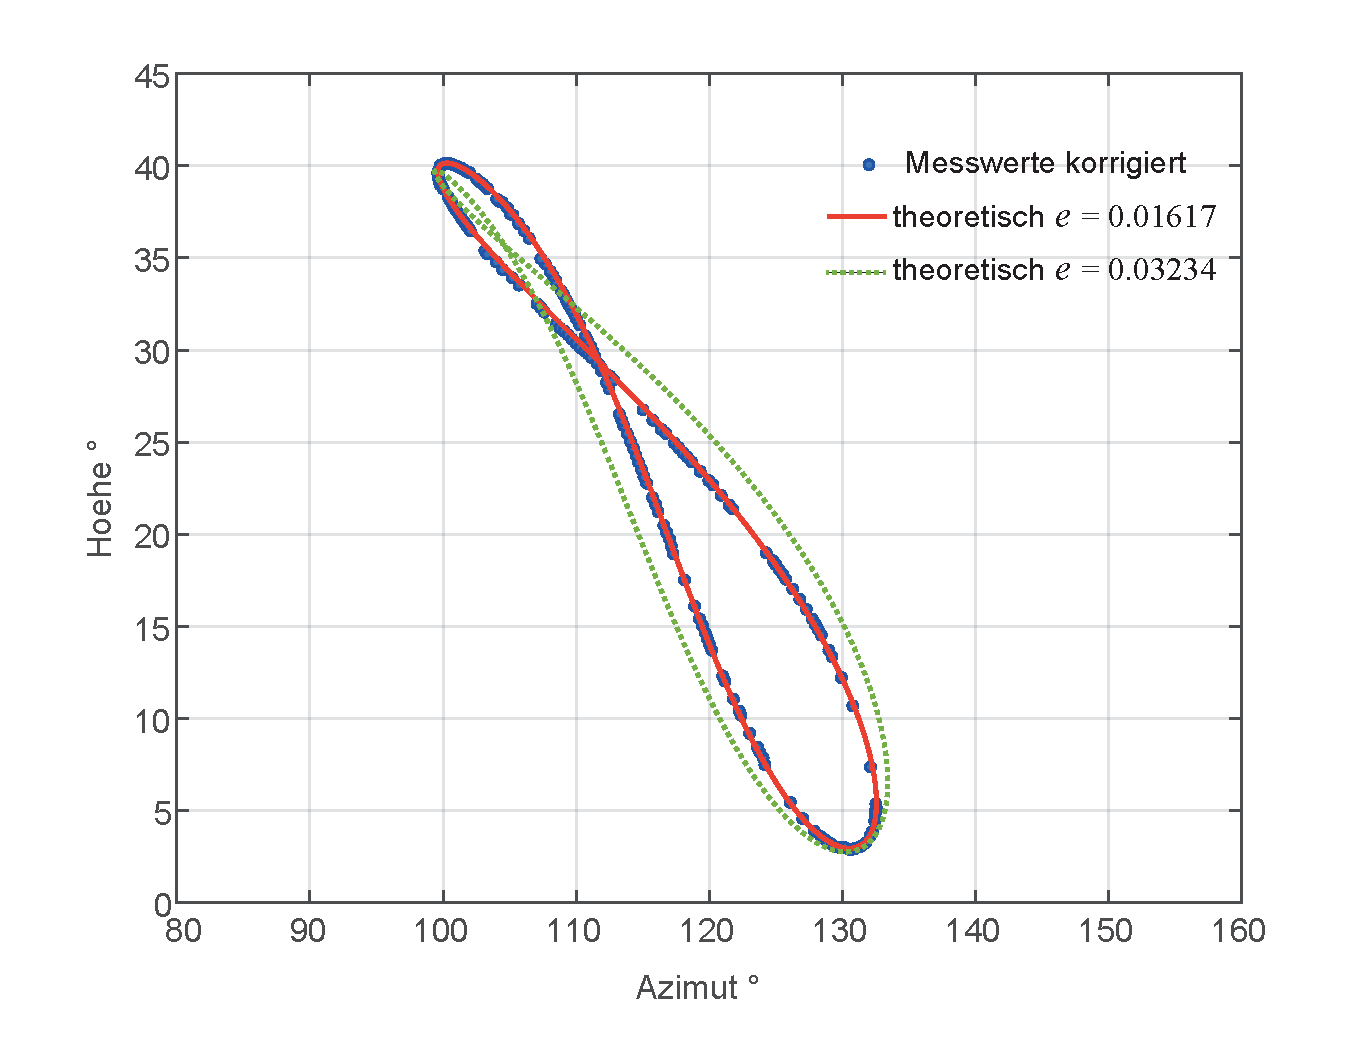
\includegraphics[width=1.0\textwidth]{Analemmafit.pdf}
\caption[Aufnahme eines Analemmas in den Jahren 2019/2020.]{Aufnahme eines Analemmas in den Jahren 2019/2020  und Fit mit der Exzentrizit�t als Parameter (Modellierung ausgef�hrt in den \mscr en \mlhmref{AnalemmaOkoFit.m} und \mlhmref{AnalemmaFindExz.m}).}
\label{abb:hm_Analemma_02}
\end{figure}

In \figref{hm_Analemma_03} haben wir noch schlie�lich berechnete Analemmas f�r zwei Standorte auf der Erde f�r verschiedene Tageszeiten dargestellt.
Man beachte die Effekte des Polarsommers \bzw Polarwinters auf das Analemma von Troms�.

\begin{figure}
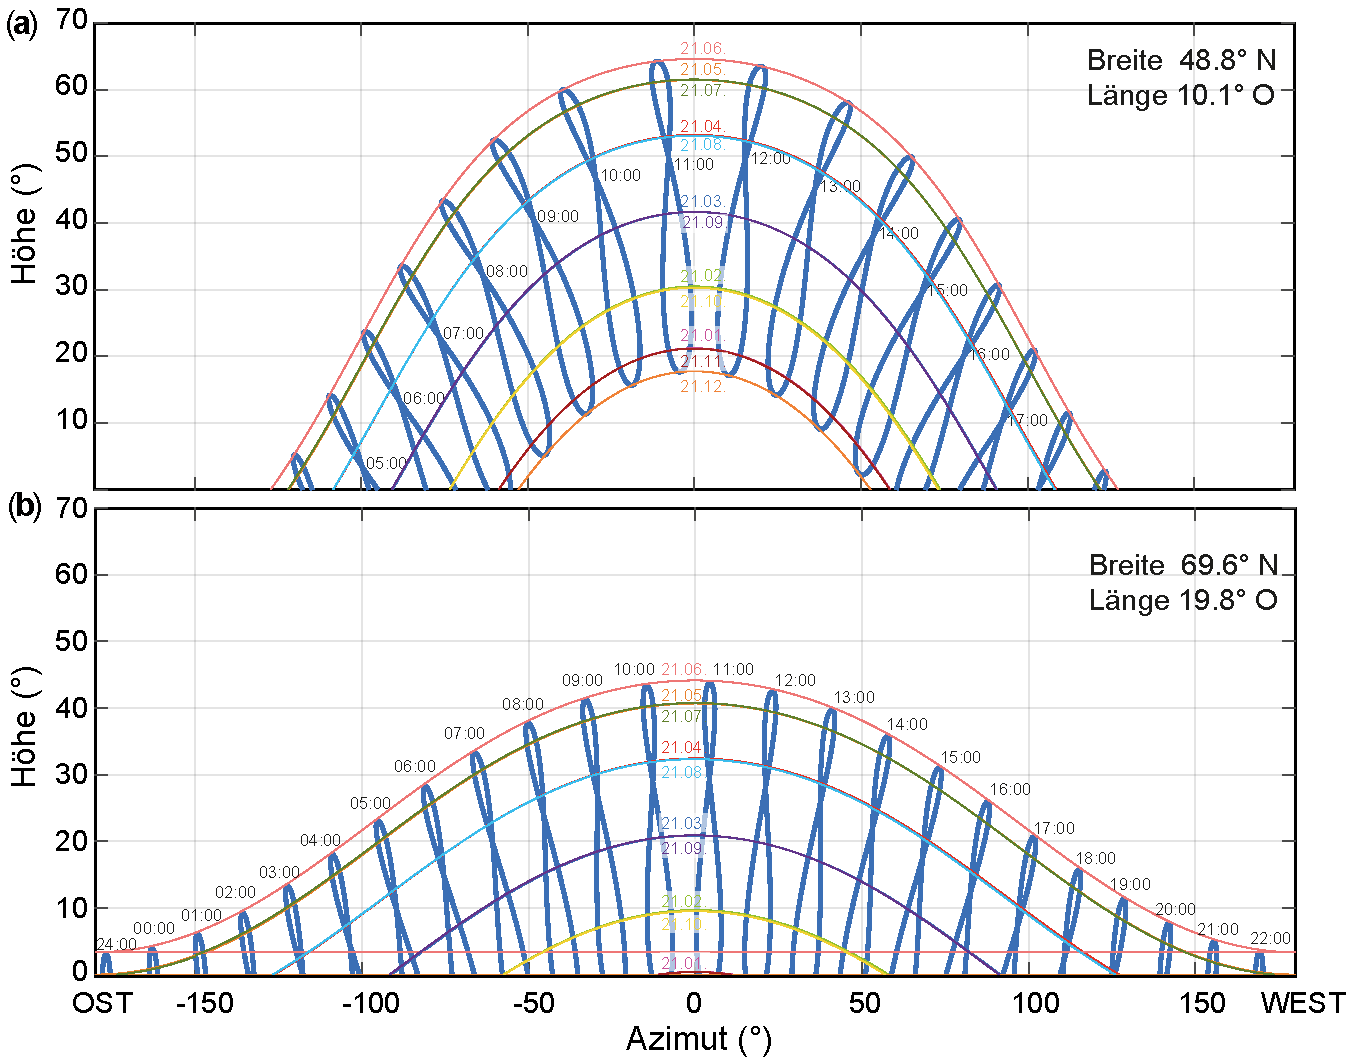
\includegraphics[width=1.0\textwidth]{Analemma03.pdf}
\caption[Berechnete Analemma-Bilder f�r zwei geographische Orte.]{Berechnete Analemma-Bilder f�r Oberkochen, Deutschland \fa und Troms�, Norwegen \fb \mscr{} (\mlhmref{Analemma02.m}).}
\label{abb:hm_Analemma_03}
\end{figure}

\subsubsection{Refraktionskorrekturen, Parallaxe}\index{Refraktionskorrektur}

Zur Berechnung von Auf- und Untergangszeiten\index{Aufgangszeiten}\index{Untergangszeiten} m�ssen wir das topozentrisch-horizontale KOS benutzen und den Stundenwinkel $\tau$ des Himmelsk�rpers bei $h\!=\!0$ mit \eqref{eq:hm_Alt-Az-Koord} berechnen.
Dabei m�ssen wir aber Einflussfaktoren wie Refraktion, Parallaxe und scheinbaren Durchmesser $D_\text{O}$ des Himmelsk�rpers ber�cksichtigen, die wir hier kurz vorstellen wollen. 

\subparagraph{\textbf{\gls{refraktion}}}
In der Astronomie ist vor allem die Ablenkung der Lichtstrahlen durch die Erdatmosph�re und die damit verbundene \anf{scheinbare} �nderung der Koordinaten von Bedeutung.
Physikalisch gesehen wird diese Brechung (Refraktion) der aus dem All kommenden Lichtstrahlen durch die optisch dichter werdenden Schichten der Atmosph�re verursacht.
Als Folge davon werden die Lichtstrahlen zur Erde hin gekr�mmt (\probref{hm_refrak_optik}).
Da Beobachter immer von einer geradlinigen Ausbreitung ausgehen, weicht die Beobachtungsrichtung vom tats�chlichen Lichtweg ab (\figref{hm_refraktion}).
Alle Objekte werden daher unter einer gr��eren H�he (der scheinbaren H�he $h'$) als der wahren, d.\,h. berechneten (sogenannten astrometrischen) H�he\index{H�he!wahre}\index{H�he!scheinbare}\index{H�he!astrometrische} $h$ gesehen.
Der Unterschied ist in Horizontn�he am gr��ten und bei der Beobachtung eines Objektes im Zenit gleich Null. 

\begin{figure}
\begin{minipage}{\textwidth}
\leftfigure{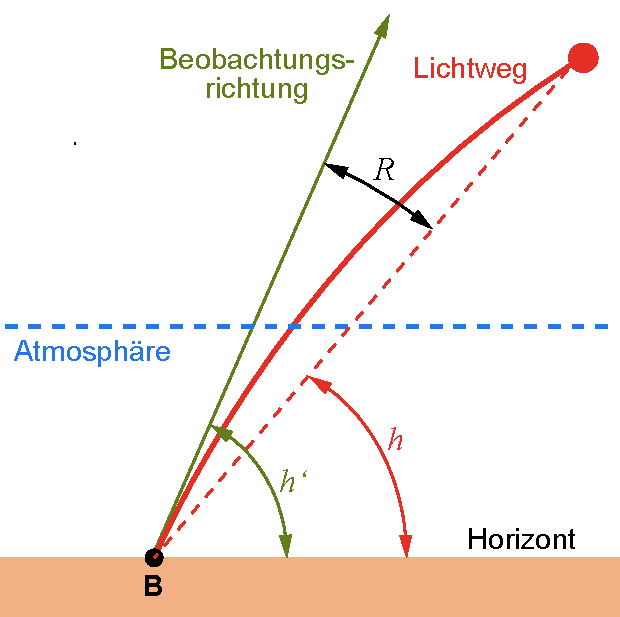
\includegraphics[width=0.5\textwidth]{Refraktion.pdf}}
\hspace{\fill}
\rightfigure{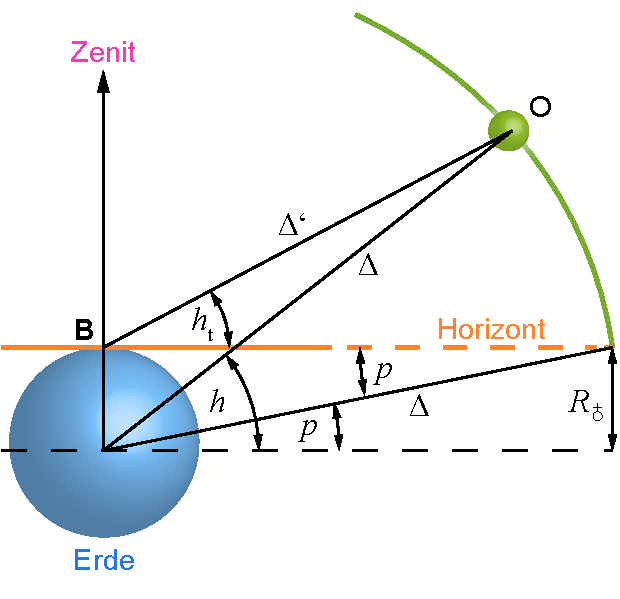
\includegraphics[width=0.5\textwidth]{TopozentrischeParallaxe.pdf}}
\leftcaption{Refraktion in der Himmelsbeobachtung.}\label{abb:hm_refraktion}
\rightcaption{Parallaxe und Horizontalparallaxe.}\label{abb:hm_parallaxe}
\end{minipage}
\end{figure}

Die sogenannte \emph{Refraktionskurve}\index{Refraktionskurve} $R(h')\!=\!R(90\degree-z')=h'-h$ gibt die Abh�ngigkeit von der scheinbaren H�he\index{H�he!scheinbare} $h'$ �ber dem Horizont bzw. von der Zenitdistanz $z'\!=\!90\degree-h'$ an.\footnote{Ungl�cklicherweise bezeichnet man die Refraktion mit $R$, was oft zu Verwechslungen mit Radien und Abmessungen f�hrt. Da in der Literatur und insbesondere in Tabellen aber $R$ benutzt wird, halten wir uns ebenfalls an die Konvention.}
Der genaue Wert h�ngt von vielen Parametern ab, \ua den Brechzahlen der Luftschichten, die wiederum eine Funktion der atmosph�rischen Bedingungen wie Druck, Temperatur und der geographischen Breite sind.
Zur Berechnung von $R(h')$ ausgehend von der scheinbaren H�he (oder alternativ $R(h)$), wurden verschiedene Modelle entwickelt (\probref{hm_refrak_optik}), woraus entsprechende Refraktionstafeln berechnet wurden.
F�r unsere Zwecke reicht zun�chst die Betrachtung der sogenannten Normalrefraktion in Horizontn�he.
Man kann dabei mit folgenden Formeln arbeiten \cite{Meeus1998}, wobei $h$ bzw. $h'$ in \textdegree\ einzusetzen sind und das Ergebnis in Bogenminuten ausgegeben wird:
\begin{equation} \label{eq:hm_Normalrefraktion1}
R(h')=h'-h=\frac{1}{\tan \lk{h'+\frac{7.31\degree}{h'+4.4\degree}}\rk} ~~~\left[ \text{Ausgabe in Bogenminuten} \right] ~,
\end{equation}
\begin{equation} \label{eq:hm_Normalrefraktion2}
R(h)=h'-h=\frac{1}{\tan\lk{h+\frac{10.3\degree}{h+5.11\degree}}\rk} ~~~ \left[ \text{Ausgabe in Bogenminumten} \right] ~.
\end{equation}

F�r die Bestimmung eines Aufgangs ist die scheinbare H�he gleich Null.
Man muss also den Zeitpunkt f�r $h\!=\!-R(h'\!=\!0)$ berechnen.
Aus \eqref{eq:hm_Normalrefraktion1} bestimmt man $R(h'\!=\!0)\!=\!34'$.
Mit diesem Wert werden wir nun weiterrechnen.

\subparagraph{\textbf{\gls{parallaxe}}}\index{Parallaxe}
Wir hatten bereits in \kapitel{hm_koordinatensysteme} auf den Unterschied zwischen einem topozentrischen und einem geozentrischen KOS hingewiesen und in Tabelle \ref{tab:hm_Umrechung_KOS} auch die Transformation zwischen beiden angegeben.
Der Unterschied zwischen beiden KOS muss dann ber�cksichtigt werden, wenn der Erdradius im Verh�ltnis zum Abstand des beobachteten Himmelsobjektes nicht mehr zu vernachl�ssigen ist.
Das ist auf alle F�lle beim Mond im Verh�ltnis zur Erde, aber auch den inneren Planeten und unter Umst�nden (\zb bei Berechnung von Sonnenfinsternissen) bei der Sonne der Fall.
Durch die Parallaxe ist die topozentrische H�he $h_\text{t}$ kleiner als die geozentrisch (berechnete) H�he $h_\text{g}$.
Die Parallaxe wirkt also der Refraktion entgegen.
Wir k�nnen f�r $h_\text{t}\!=\!0$ die sogenannte Horizontalparallaxe aus \figref{hm_parallaxe} bestimmen zu
\begin{equation} \label{eq:hm_Parallaxe}
p=\arcsin\lk \frac{R_\text{\earth}}{\Delta} \rk ~.
\end{equation}
F�r die Sonne berechnet sich ein Betrag von etwa 9'' (Bogensekunden), f�r den Mond schon betr�chtliche 57' (Bogenminuten).
Die Parallaxe ist also beim Mond definitiv nicht mehr zu vernachl�ssigen.


\subparagraph{\textbf{Scheinbarer Durchmesser}}\index{Durchmesser!scheinbarer|textbf} 
F�r die Aufgangsberechnung haben wir au�erdem noch den Winkeldurchmesser $D_\text{O}$ des Himmelsobjektes zu ber�cksichtigen, unter dem dieses von der Erde aus erscheint.
Wir messen bei Aufg�ngen das Erscheinen des oberen Rands, m�ssen also $R_\text{O}\!=\!D_\text{O}/2$ in der Berechnung der Aufgangsh�he ber�cksichtigen.
Mit $D_\text{O \astrosun} = 32'$ und $D_\text{O M} = 29' \ldots 34'$ ergibt sich insgesamt f�r die Korrektur der H�he
\begin{equation}\label{eq:hm_Parallaxe_2}
h_\text{A,U}=0\text{\textdegree}-R\lk h'=0 \rk +p-R_\text{O} =  \begin{cases} -50' ~~ &\text{Sonne} \\ +\; 6' \ldots 8' ~~ &\text{Mond}\end{cases}  ~.
\end{equation}


\subsubsection{Berechnung der Auf- und Unterg�nge} \label{kap:auf-untergaenge}\index{Aufg�nge}\index{Unterg�nge}
Wir k�nnten nun $h_\text{A,U}$ aus \eqref{eq:hm_Parallaxe_2} in \eqref{eq:hm_Alt-Az-Koord} einsetzen und den Stundenwinkel $\tau$ bzw. die Sternzeit $\theta$ bestimmen, woraus sich wiederum die Ortszeit f�r den Auf- \bzw Untergang bestimmen l�sst.
Da aber bei der Sonne sowohl Rektaszension $\alpha$ als auch Deklination $\delta$ selbst zeitabh�ngig sind, k�nnen wir die transzendente Bestimmungsgleichung \eqref{eq:hm_Alt-Az-Koord} nicht analytisch, sondern nur mittels numerischer Verfahren l�sen.
Dazu geht man iterativ vor:
\begin{enumerate}
	\item Man startet mit der Berechnung der \gls{sternzeit} $\theta_i$ f�r $t_i\!=$ 12:00 UT aus dem Datum und der geographischen L�nge.
          Man berechnet daraus die Deklination $\delta_i$ und die Rektaszension $\alpha_i$, die die Sonne zu dieser Zeit hat.
          Daraus ergibt sich der Stundenwinkel $\tau_i\!=\!\theta_i-\alpha_i$. 
	\item Wir berechnen dann den Stundenwinkel $T_i$ aus \eqref{eq:hm_Alt-Az-Koord} und daraus eine neue Uhrzeit $t_{i+1}$ f�r den Auf- bzw. Untergang mittels
\begin{align}
T_i &= \pm \lk \frac{1^\text{h}}{15\degree} \rk \arccos\lk \frac{\sin h_\text{A,U}-\sin\delta(\tau_i)\sin\varphi}{\cos\delta(\tau_i)\cos\varphi}\rk \label{eq:hm_std_winkel_Ti} ~,\\
t_{i+1} &=t_i + (T_i-\tau_i) ~.\nonumber
\end{align}
Dabei muss man auf einige Sonderf�lle achten, z.\,B. wenn $T_i$ in \eqref{eq:hm_std_winkel_Ti} komplex wird.
Dann geht die Sonne an dem Tag nicht unter, was z.\,B. im Polarsommer in hohen geographischen Breiten der Fall sein kann. 
\end{enumerate}
Eine alternative Methode der Berechnung besteht darin, dass man f�r den Tag von 0:00 bis 24:00 in Intervallen von z.\,B. 1 h die H�he $h_\text{A,U}$ als Funktion der Ortszeit (bzw. Sternzeit) berechnet und in den Intervallen nach m�glichen Nullstellen sucht.
Dazu eignen sich numerische Nullstellenverfahren.
Wir folgen in \mlhmref{Sonnenaufgang01.m} \bzw \mlhmref{Sonnenaufgang02.m} diesem Weg (siehe auch \cite{Montenbruck1999}) und nutzen die Methode der quadratischen Interpolation.
Diese bietet den Vorteil, gegebenenfalls auch zwei Nullstellen in einem Intervall ermitteln zu k�nnen.
Das Programm ist in dieser Form auch anwendbar auf die Berechnung von Auf- und Untergangszeiten des Mondes oder von Satelliten, sofern man die Berechnungsformeln f�r deren �quatoriale Koordinaten kennt. 

Das Ergebnis einer Sonnenauf- und -untergangs-Berechnung ist in \figref{hm_Sonnenauf_untergang} f�r Oberkochen ($\phi\!=\!48.8\degree$ und $\lambda\!=\!10.1\degree$) zu sehen.
Man erkennt in der vergr��erten Darstellung (rechtes Bild) sehr sch�n, dass der k�rzeste Tag des Jahres wegen der ZGL weder mit dem fr�hesten Sonnenuntergang noch auch mit dem sp�testen Sonnenaufgang zusammenf�llt.

\begin{figure}%
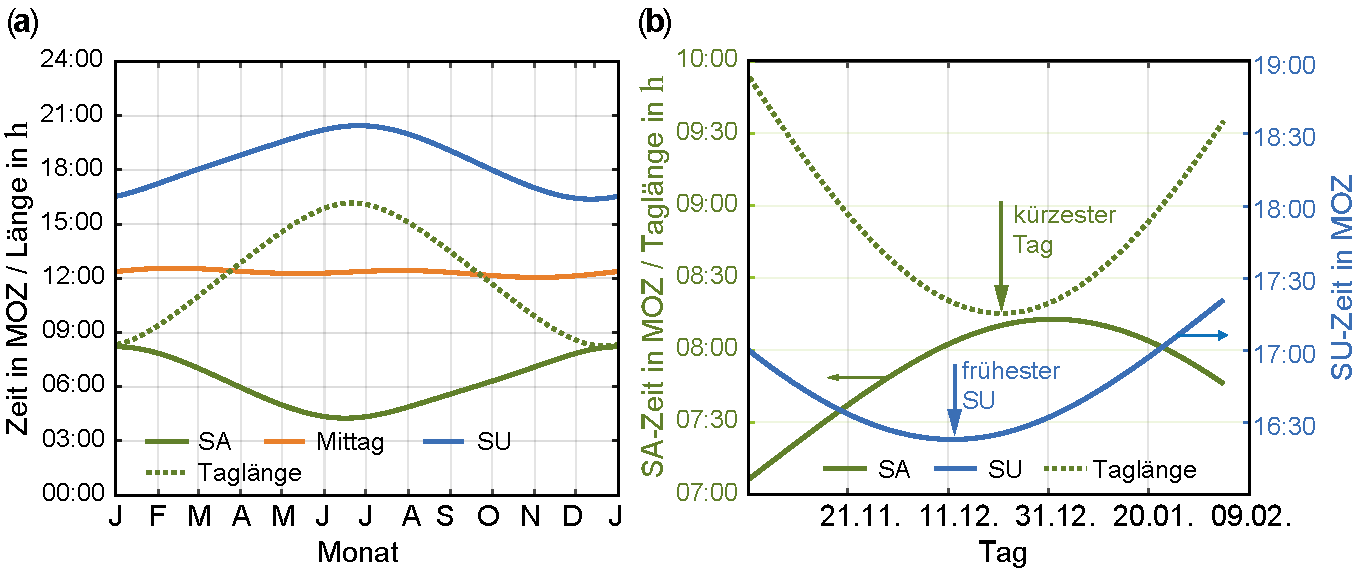
\includegraphics[width=\textwidth]{Sunrise01.pdf}\\%
\caption[Berechnung der Sonnenaufgangs- und Sonnenuntergangszeiten.]{Berechnung der Sonnenaufgangs- und Sonnenuntergangszeiten. \fa SA, SU, Tagl�nge in Oberkochen (Breite $\phi\!=\!48.8\degree$ und L�nge $\lambda\!=\!10.1\degree$). \fb SA, SU und Tagl�nge um den Jahreswechsel. Die $x$-Achse in \fa ist mit den Anfangsbuchstaben der Monate bezeichnet.}%}%
\label{abb:hm_Sonnenauf_untergang}%
\end{figure}

\subsubsection{N�herungsformeln und deren Herleitung} \label{kap:hm_naeherungsformeln_sonne}
\subparagraph{\textbf{Reihenentwicklung der Zeitgleichung}}
Wir wollen jetzt handhabbare Formeln f�r die Zeitgleichung sowie Auf- und Untergangszeiten der Sonne herleiten.
Dazu starten wir mit der geozentrischen Darstellung in \figref{hm_wahre_sonne_geoz}. 
\begin{figure}%
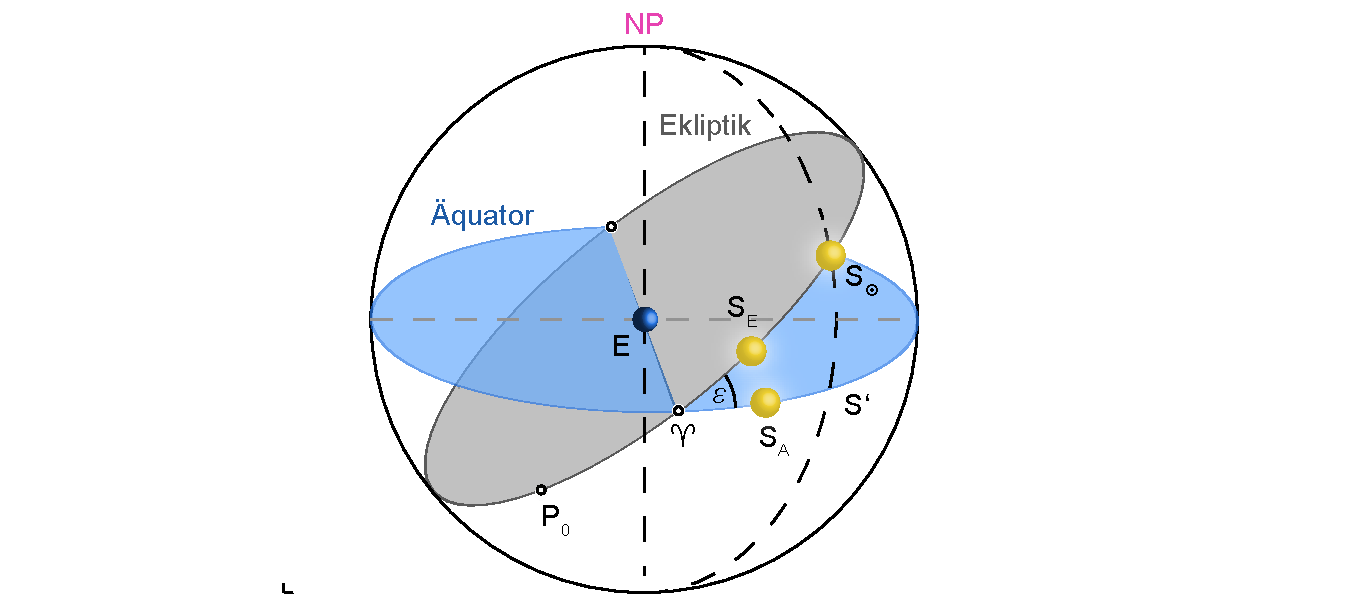
\includegraphics[width=\textwidth]{Wahre_und_mittlere_Sonne.pdf}%
\caption{Bewegung der wahren und der mittleren Sonne im geozentrischen Bild.}%
\label{abb:hm_wahre_sonne_geoz}%
\end{figure}
In dieser Abbildung haben wir neben der \anf{wahren} Sonne $\text{S}_\text{\astrosun}$ zwei weitere \anf{Hilfssonnen} $\text{S}_\text{E}$ und $\text{S}_\text{A}$ eingezeichnet.
Die Sonne $\text{S}_\text{A}$ bewege sich mit konstanter Umlaufgeschwindigkeit in der �quatorebene und die Sonne $\text{S}_\text{E}$ ebenfalls mit konstanter Winkelgeschwindigkeit auf der Ekliptik.
Die wahre Sonne $\text{S}_\text{\astrosun}$ bewege sich entlang der Ekliptik entsprechend der Keplergesetze mit ver�nderlicher Geschwindigkeit.
Die Hilfssonnen sind so definiert, dass beide mit der wahren Sonne in den �quinoktien\index{Aequinoktium@�quinoktium} \glslink{aequinox} zusammentreffen.
In \figref{hm_wahre_sonne_geoz} sind die geozentrischen Parameter entsprechend denen des heliozentrischen Bildes von \figref{hm_planetenbahnen_rel_ekliptik} definiert.
\begin{align*}
\lambda_\text{\astrosun}&=\angle\vernal\text{ES}_\text{\astrosun}       ~&\text{L�nge der wahren Sonne} \\
\Lambda_\text{M}&=\Lambda_\text{\astrosun}=\angle\vernal\text{ES}_\text{E}~&\text{L�nge der mittleren Sonne}  \\
\alpha_\text{\astrosun}&=\angle\vernal\text{ES'}          ~&\text{Rektaszension der wahren Sonne}  \\
\alpha_\text{M}&=\angle\vernal\text{ES}_\text{A}          ~&\text{Rektaszension der mittleren Sonne}  \\
\upsilon&=\lambda_\text{\astrosun}-\varpi=\angle\text{P}_0\text{ES}_\text{\astrosun}  ~&\text{wahre Anomalie}  \\
M&=\Lambda_\text{\astrosun}-\varpi=\angle\text{P}_0\text{ES}_\text{E}~&\text{mittlere Anomalie}
\end{align*}

Da die beiden Hilfssonnen mit gleicher Geschwindigkeit umlaufen, gilt $\Lambda_\text{\astrosun}\!=\!\alpha_\text{M}$.
Mit der Definition der Zeitgleichung \eqref{eq:hm_tau_zgl} erh�lt man
\begin{align}
\begin{split}  
\tau_\text{ZGL} &= \text{WOZ} - \MOZ = (\theta - \alpha_\text{\astrosun}) - \underbrace{(\theta-\alpha_\text{M})}_{0} = \alpha_\text{M}-\alpha_\text{\astrosun} = \Lambda_\text{\astrosun}-\alpha_\text{\astrosun} \\ 
&= (\Lambda_\text{\astrosun} - \lambda_\text{\astrosun}) + (\lambda_\text{\astrosun}-\alpha_\text{\astrosun}) = (\Lambda_\text{\astrosun} + \varpi) - (\lambda_\text{\astrosun}+\varpi)+(\lambda_\text{\astrosun}-\alpha_\text{\astrosun})  \\
&=\underbrace{(\Lambda_\text{\astrosun}-\varpi) - (\lambda_\text{\astrosun}-\varpi)}_{-\mathcal{C}\text{, siehe \eqref{eq:hm_mpglg_nu-M}}} + \underbrace{(\lambda_\text{\astrosun} -\alpha_\text{\astrosun})}_{\text{Reduktion $\mathcal{R}$, siehe \eqref{eq:hm_reduktions_formel4}}} \,. 
\end{split} \label{eq:hm_tau_ZGL_C}
\end{align}
Die ersten beiden Terme ergeben also den negativen Wert der Mittelpunktsgleichung.
Der dritte Term ist die sogenannte \emph{\gls{reduktion}}\index{Reduktion} der Ekliptik auf den �quator, \dh die Differenz zwischen bekannter ekliptikaler L�nge und gemessener �quatorialer Rektaszension.
Die Herleitung dieser Reduktion, die nur von $\lambda_\text{\astrosun}$ und $\epsilon$ abh�ngt, ist in \kapitel{reduktion_ekliptik} in Beispiel \ref{bsp:herleitung_redformel_ekl} detailliert ausgef�hrt. 
Wir benutzen hier das Ergebnis der Rechnung und erhalten 
\begin{align}
\begin{split}
\tau_\text{ZGL} &= -C+(\lambda_\text{\astrosun}-\alpha_\text{\astrosun}) \\
                &= -C+\tan^2\lk\frac{\epsilon}{2}\rk \sin(2\lambda_\text{\astrosun})-\frac{1}{2}\tan^4 \lk \frac{\epsilon}{2}\rk \sin(4\lambda_\text{\astrosun})+\mathcal{O}\lk \tan^6 \lk \frac{\epsilon}{2} \rk\rk \,. 
\end{split} \label{eq:hm_tau_ZGL_C1}
\end{align}
Man kann sich also merken: Die \emph{Zeitgleichung} ist die Summe von (negativer) Mittelpunktsgleichung (\emph{Wirkung der Exzentrizit�t}) und Reduktion der Ekliptik\index{Reduktion!auf den �quator} auf den �quator (\emph{Wirkung der Ekliptikschiefe}).
Wir wollen jetzt in der Form der ZGL \eqref{eq:hm_tau_ZGL_C1} die i.\,A. nicht bekannte ekliptikale L�nge der wahren Sonne $\lambda_\text{\astrosun}$ durch die tabellierte bzw. die einfach berechenbare L�nge $\Lambda_\text{\astrosun}$ der mittleren Sonne ersetzen.
Wir k�nnen dabei folgende Beziehungen nutzen:
\begin{align*}
\lambda_\text{\astrosun} &= \Lambda_\text{\astrosun} + \mathcal{C} =\Lambda_\text{\astrosun}+2e\sin M + \frac{5}{4}e^2\sin(2M) +\mathcal{O}(e^3) \,,\\
\sin(2\lambda_\text{\astrosun}) &\approx \sin(2\Lambda_\text{\astrosun})+4e\sin M \cos(2\Lambda_\text{\astrosun}) +\mathcal{O}(e^3)\,,\\
\sin(4\lambda_\text{\astrosun}) &\approx \sin(4\Lambda_\text{\astrosun}) + \mathcal{O}(e^3)\,.
\end{align*}
Mit der Abk�rzung $y=\lek\tan\lk\frac{\epsilon}{2}\rk\rek^2$ erhalten wir dann
 \begin{align*}
\tau_\text{ZGL} &= -\mathcal{C} + \underbrace{y \sin(2\Lambda_\text{\astrosun})- \frac{1}{2} y^2 \sin(4\Lambda_\text{\astrosun})}_{\text{T}_\text{I}} + 
\underbrace{4 e y \cos(2\Lambda_\text{\astrosun}) \sin(M)}_{\text{T}_\text{II}}  ~.\label{eq:hm_tau_ZGL_D}
\end{align*}
Der Term $\mathcal{C}$ beschreibt wie bereits erw�hnt den Effekt der Exzentrizit�t, der Term $T_\text{I}$ den der Schiefe der Ekliptik; er verschwindet mit $\epsilon \rightarrow 0$.
Term  $T_\text{II}$ ist ein Mischterm.
$\Lambda_\text{\astrosun}$ ist in einschl�gigen Tabellen (siehe auch Tabelle \ref{tab:hm_bahnparameter} im Anhang) aufgef�hrt.
Wir ersetzen $M = \Lambda_\text{\astrosun} - \varpi$ und erhalten mit 
\begin{equation*}
\Lambda_\text{\astrosun} = n(t-t_0) + \Lambda_\text{\astrosun 0} = 359999.0498\degree \:t + 280.4656\degree ~~
\end{equation*}
und den bekannten Beziehungen f�r trigonometrische Funktionen die Zeitgleichung in der folgenden Form:
\begin{align}
\tau_\text{ZGL} &= \sum_{k} \alpha_k \sin(k\Lambda_\text{\astrosun}) + \beta_k\cos(k\Lambda_\text{\astrosun}) = \sum_{k} \gamma_k\sin(\kappa_k t+\delta_k)\,, \label{eq:hm_parameter_alpha_beta} 
\end{align}
wobei
\begin{align*}
\kappa_k &= kn\,\frac{2\pi}{360\cdot 36525}~, \:\gamma_k = -\frac{24\cdot 60}{2\pi}\sqrt{\alpha_k^2+\beta_k^2}~~\: \text{und} \\
\delta_k &= k \, \Lambda_{\astrosun,0}+\arctan\lk \frac{\beta_k}{\alpha_k}\rk -\pi ~.
\end{align*}
Die Koeffizienten der Summen $\alpha_k$, $\beta_k$ bzw. $y_k$, $\delta_k$, $\kappa_k$ sind Funktionen der Bahnparameter der Erde $e$, $\varpi$, $n$, $\Lambda_\text{\astrosun,0}$, sowie der Ekliptikschiefe $\epsilon$ und damit auch abh�ngig von der Zeit.\footnote{Wir kommen darauf in \kapitel{hm_langezeiten} zur�ck.
Man beachte, dass in \eqref{eq:hm_parameter_alpha_beta} nur die Entwicklung bis zur Ordnung $e^2$ enthalten ist.} Wir rechnen mit den Werten f�r das �quinoktium des Datums, $t$ sind wiederum die seit J2000 vergangenen Jahrhunderte.
Die Koeffizienten $y_k$ sind in Zeitsekunden umgerechnet und f�r die Sinus-Funktion nutzen wir $\sin(x-\pi)\!=\!-\sin x$.
F�r die Parameter $\alpha_k$, $\beta_k$ bis $k\!=\!4$ erhalten wir
\begin{align}
\begin{split}
\alpha_1 &= -2e\cos\varpi -2e\tan^2\lk\frac{\epsilon}{2}\rk\cos\varpi \,, ~~~\beta_1 = +2e\sin\varpi-2e\tan^2\lk\frac{\epsilon}{2}\rk\sin\varpi \,,   \\ 
\alpha_2 &= -\frac{5}{4}e^2\cos(2\varpi) +\tan^2\lk\frac{\epsilon}{2}\rk \,, ~~~\beta_2 = +\frac{5}{4}e^2\sin(2\varpi)\,,  \\
\alpha_3 &= +2e\tan^2\lk\frac{\epsilon}{2}\rk\cos\varpi \,, ~~~\beta_3 = -2e \tan^2\lk\frac{\epsilon}{2}\rk\sin \varpi \,, \\
\alpha_4 &= -\frac{1}{2}\tan^4\lk\frac{\epsilon}{2}\rk \,,  ~~~\beta_4 = 0 \,. 
\end{split}\label{eq:hm_parameter_alpha_beta2}
\end{align}
Daraus berechnen wir mit den Bahnparametern aus Tabelle \ref{tab:hm_bahnparameter} die Zeitgleichung in der �blichen Form: 
\begin{align}
\tau_\text{ZGL} &=\! 7.364186\,\sin(0.017202\, t_\text{d}-0.062882) \nonumber  \\
								& \!-9.93481\,\sin(0.034404\, t_\text{d} + 0.368790) + \ldots \label{eq:hm_ZGL21}
\end{align}
mit
\begin{align*}
y_k      &= \! (-7.364186,\,-9.93481,\,-0.329614,\,-0.21222, \ldots) ~~\text{in Zeitminuten,} \\
\kappa_k &= \! (0.017202,\,0.034404,\,0.051606,\,0.068808, \ldots) ~~\text{im Bogenma�,} \\
\delta_k &= \! (-0.062882,\,0.361758,\,0.321940,\,0.730548,\ldots) ~~\text{im Bogenma�}. 
\end{align*}
Hierin haben wir die Parameter $\kappa_k  \rightarrow 100 \kappa_k$ und $t\!\rightarrow \!t_\text{d}$ mit $t_\text{d} = 0 \ldots 365$ f�r die Tage eines Jahres gesetzt, was wegen der Periodizit�t in $\kappa_k$ f�r das Jahr 2000 streng gilt, f�r Jahre um 2000 n�herungsweise.\footnote{F�r andere Jahre muss man die Parameter \eqref{eq:hm_parameter_alpha_beta2} neu berechnen, siehe auch \kapitel{hm_altertum_zeiten}.} Dies ist die allgemein bekannte und gut handhabbare Form der Zeitgleichung.
Die ersten beiden Terme zeigen �ber \eqref{eq:hm_parameter_alpha_beta2} die Beitr�ge der Exzentrizit�t und der Ekliptikschiefe (\figref{hm_reihenent_zeitglg}).
Zur Verdeutlichung sind die deutlich kleineren Terme mit $3\omega$ und $4\omega$ jeweils um einen Faktor 10 vergr��ert dargestellt.
Da wir in unserer Berechnung wiederum sechs Bahnparameter (inklusive der Zeit $T_0$) benutzt haben, muss man die Reihe mindestens bis $k\!=\!2$ entwickeln, was meist schon ausreichend genaue Ergebnisse liefert.
Alle in der Literatur vorhandenen und leicht unterschiedlichen Zeitgleichungen basieren letztendlich auf dieser Grundform.
Sie unterscheiden sich in der Wahl des �quinoktiums und der Ordnung $k$ der Reihenentwicklung.
In \mlhmref{ZGL03.m} sind die verschiedenen publizierten Zeitgleichungen \cite{Wetzel2007,Rempel2019} miteinander verglichen.
\begin{figure}%
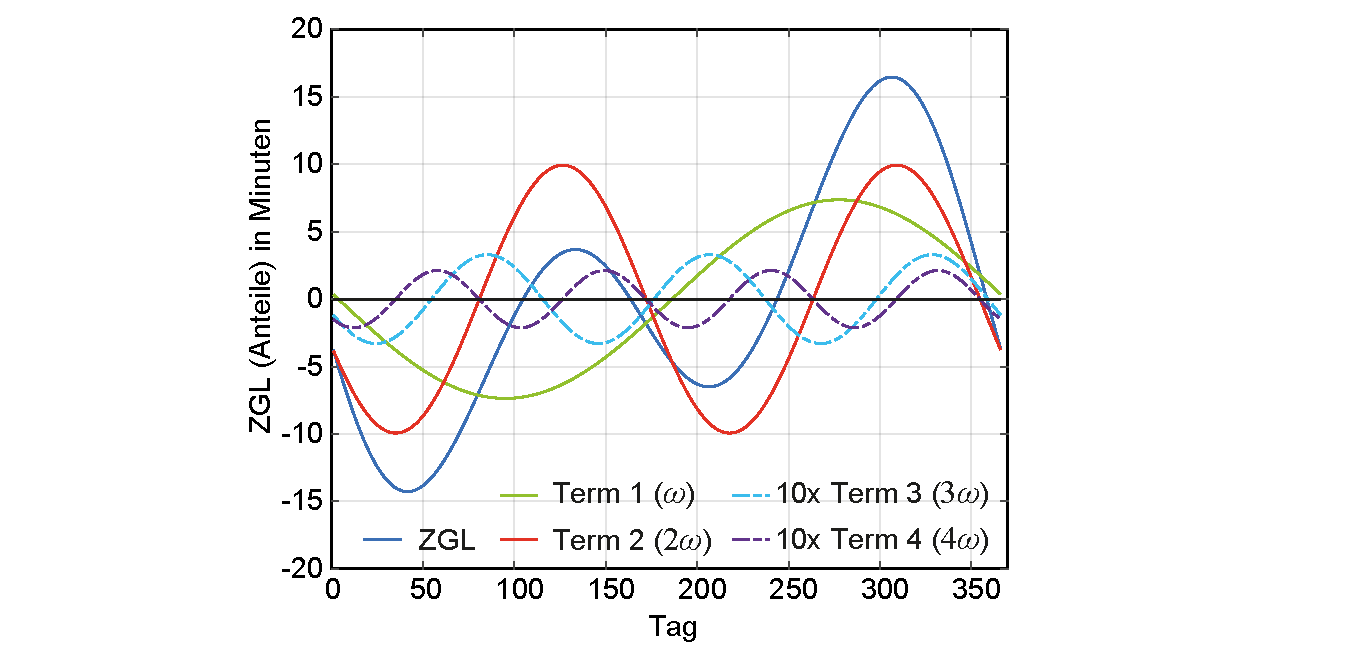
\includegraphics[width=\textwidth]{ZGL02.pdf}%
\caption{Reihenentwicklung der Zeitgleichung.}%
\label{abb:hm_reihenent_zeitglg}%
\end{figure}

Nach gleicher Methodik kann auch die Deklination als Funktion der seit einem Zeitpunkt vergangenen Tage $t_\text{d}$ berechnet werden.
Wir geben hier nur das erste Glied der Reihenentwicklung im Bogenma� an:
\begin{equation}
\delta(t_\text{d}) = 0.4095 \, \sin(0.016906 t_\text{d} - 1.35393) \,. \label{eq:hm_delta_von_T_hash}
\end{equation}

\subparagraph{{N�herungsformel f�r den Sonnenaufgang und Sonnenuntergang}}\index{Sonnenaufgang}\index{Sonnenuntergang}
Mit den beiden letzten Formeln wollen wir nun ebenfalls Berechnungsformeln f�r den Sonnenaufgang \bzw -untergang herleiten.
Wir haben in \kapitel{auf-untergaenge} zur Bestimmung des Aufgangs eines Himmelsk�rpers mit zeitlich ver�nderlicher Deklination und Rektaszension (wie z.\,B. Sonne und Mond) eine numerische Methode w�hlen m�ssen, weil es gem�� \eqref{eq:hm_Alt-Az-Koord} keine geschlossene Umkehrfunktion $\tau(h)$ zur Funktion $h(\tau)$  gibt.
Da sich aber die Deklination der Sonne im Verlauf eines Tages nur geringf�gig �ndert, lassen sich bei bekannter Zeitgleichung die Zeitpunkte f�r die Auf- und Unterg�nge der Sonne n�herungsweise mit relativ einfachen Formeln bestimmen, ohne dass man auf den mathematisch-numerischen Apparat f�r die iterative L�sung zur�ckgreifen muss.
Da der Kulminationszeitpunkt\glslink{kulmination}\ �ber die ZGL bekannt ist und die Deklination der Sonne innerhalb von $\pm 9$ h um den Kulminationszeitpunkt herum als n�herungsweise konstant angenommen werden kann, muss man nur noch den Schnittpunkt des Tagbogens der Sonne mit dem Horizont berechnen.
Als \emph{\gls{tagbogen}} wird der geometrische Bogen bezeichnet, den die Sonne (bzw. jeder andere Himmelsk�rper) �ber dem Horizont beschreibt.
\begin{figure}%
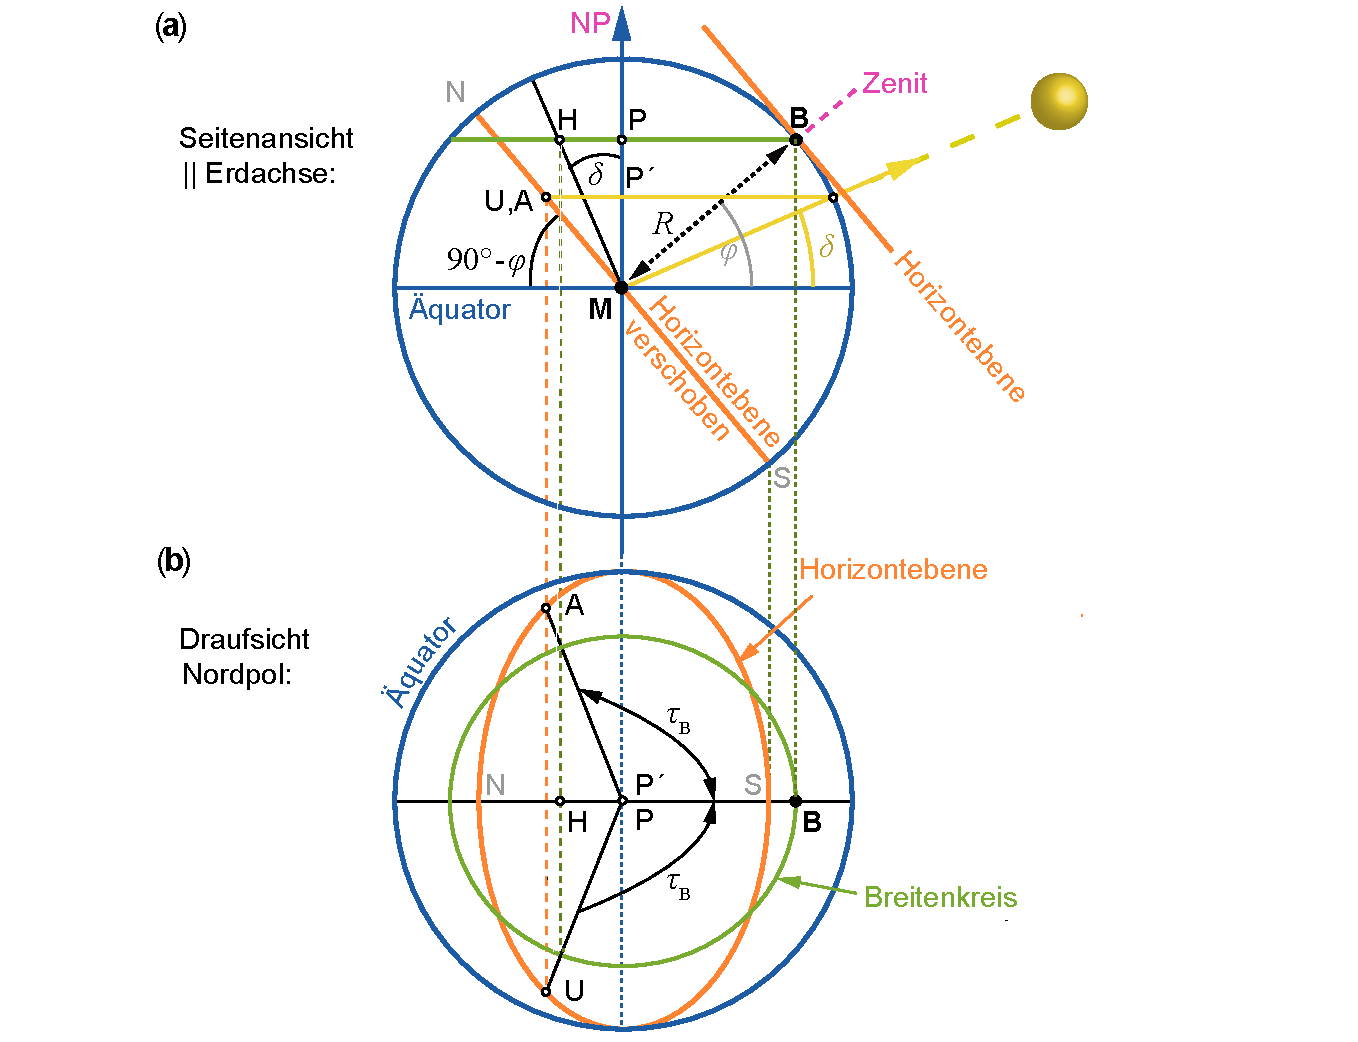
\includegraphics[width=\textwidth]{TagbogenGeometrie02.pdf}%
\caption[Geometrie des Tagbogens der Sonne.]{Geometrie des Tagbogens der Sonne (nach \cite{Praxl2016}) -- B Beobachter, A/U Auf- bzw. Untergangspunkt der Sonne am Horizont, N/S Nord-S�d-Richtung am Horizont. }%
\label{abb:hm_geom_tagbogen}%
\end{figure}
Wir betrachten dazu \figref{hm_geom_tagbogen} und k�nnen aus der Teilabbildung a direkt die folgenden Beziehungen ablesen:
\begin{align*}
\overline{\text{PM}} &= R \sin\varphi  = \overline{\text{PB}} \tan\varphi \,, \\
\overline{\text{PH}} &= \overline{\text{PM}} \tan\delta \,, \\
\rightarrow \frac{\overline{\text{PH}}}{\overline{\text{PB}}} &= \tan\varphi \tan\delta ~.
\end{align*}
Andererseits folgt aus der Teilabbildung b f�r den halben Tagbogen $\tau_\text{B}$ :
\begin{align}
\cos \tau_\text{B} \!&=\!-\cos(180\degree - \tau_\text{B}) = - \frac{\overline{\text{PH}}}{\overline{\text{PB}}} = -\tan\varphi\tan\delta ~~ \text{und somit} \nonumber \\
\tau_\text{B}\!&=\!\arccos(-\tan\varphi\tan\delta) ~.	\label{eq:hm_tau_B}
\end{align}
F�r die Aufgangszeiten erfolgt die Umrechnung von $\tau_\text{B}$ in Zeitstunden durch Multiplikation von $24 \text{h}/2\pi$.
Im Interesse �bersichtlicher Notation lassen wir die Umrechnungsfaktoren vom Bogenma� ins Zeitma� weg und gehen davon aus, dass $\tau_\text{B}$ genauso wie $\tau_\text{\,ZGL}$ in der jeweils f�r die Formel richtigen Einheit benutzt werden.
Bei der Benutzung von \eqref{eq:hm_tau_B} f�r die Aufgangszeiten\footnote{Die Formel \eqref{eq:hm_tau_B} gilt nur f�r $\abs{\tan\varphi\tan\delta}\!<\!1$, ansonsten wird der Himmelsk�rper zirkumpolar und geht weder auf noch unter, was im Sommer \zb in Breiten n�rdlich des Polarkreises f�r die Sonne der Fall ist.} m�ssen wir das Vorzeichen von $\tau_\text{B}$ beachten.
Zur Klarheit addieren oder subtrahieren wir $\abs{\tau_\text{B}}$ zur Kulminationszeit und erhalten dann f�r die Auf-/Untergangszeitpunkte 
\begin{equation}
t_\text{A,U} = \text{12:00 h} \,\text{UT} - \frac{\lambda}{15}+ \tau_\text{ZGL} + \tau_\text{A,U} ~~\text{mit}~~ \tau_\text{A} = -\abs{\tau_\text{B}} \text{ bzw. } \tau_\text{U} = \abs{\tau_\text{B}} \,. \label{eq:hm_untergangszeitp}
\end{equation}
Man ber�cksichtige, dass $\abs{\tau_\text{B}}$ in \eqref{eq:hm_untergangszeitp} von der Deklination $\delta$ nach \eqref{eq:hm_ZGL21} abh�ngt und somit ebenso wie $\tau_\text{ ZGL}$ vom jeweiligen Tag.
Jetzt m�ssen wir aber noch den Effekt der Refraktion und des scheinbaren Durchmessers der Sonne ber�cksichtigen.
Wir nehmen wieder die Refraktion in Horizonth�he mit $R\!=\!34'$ an, den scheinbaren Radius der Sonne mit $d_\text{\astrosun}/2=16'$ und vernachl�ssigen die Parallaxe.
In erster N�herung ist dann der beobachtete Tagbogen in Horizontn�he gegen�ber dem geometrisch-astronomischen (wahren) Tagbogen parallel verschoben (\figref{hm_verl_tagbogen_ref}), was zu einer Nordverschiebung des Azimuts beim Sonnenaufgang f�hrt.
Damit einher geht eine Tagbogenverl�ngerung\index{Tagbogenverl�ngerung} $\Delta\tau_\text{B}$, \dh die Sonne ist wegen der Refraktion fr�her am Himmel sichtbar als es rein geometrisch-astrometrisch der Fall w�re.
Die (halbe) Tagbogenverl�ngerung ist die Zeit, die die Sonne br�uchte, um die H�he $h_r\!=\!R+d_\text{\astrosun}/2$ zu durchlaufen.
Wir starten gem�� \eqref{eq:hm_Alt-Az-Koord} mit
\begin{equation*}
\sin h(t) = \cos\delta(t) \cos\tau \cos\varphi + \sin\delta(t)\sin\varphi ~~\text{und}~~0<t<24\:\text{h} \,.
\end{equation*}

\begin{figure}%
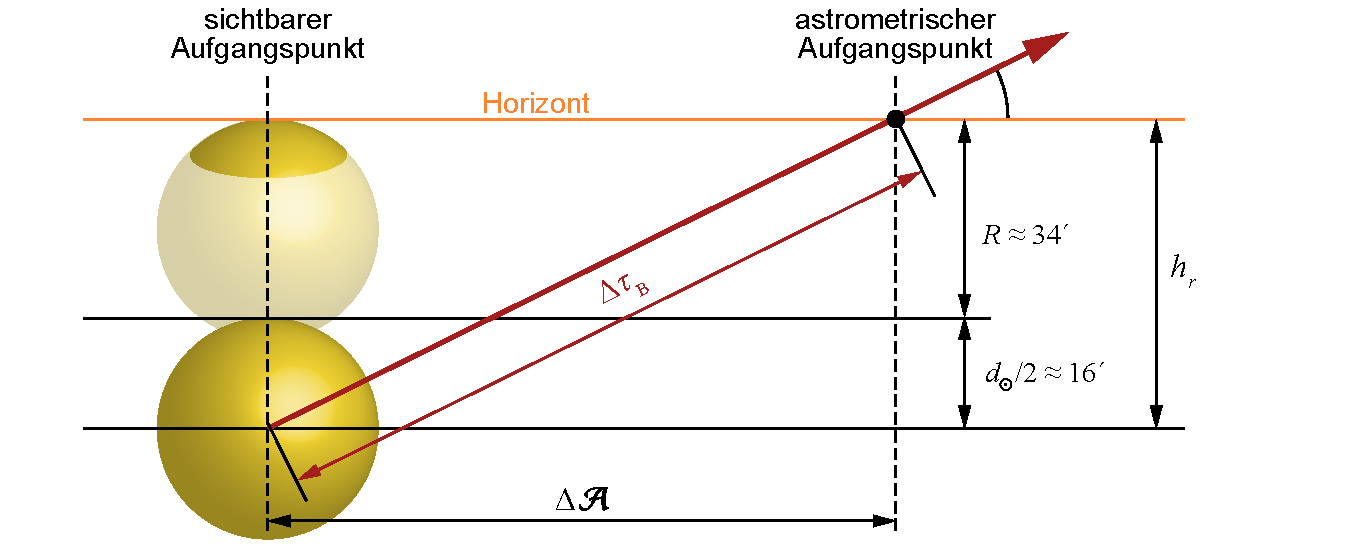
\includegraphics[width=\textwidth]{Tagbogenverlaengerung.pdf}%
\caption[Tagbogenverl�ngerung durch Refraktion und scheinbaren Durchmesser.]{Verl�ngerung des Tagbogens durch Refraktion und scheinbaren Durchmesser.}%
\label{abb:hm_verl_tagbogen_ref}%
\end{figure}

Ber�cksichtigen wir, dass $\D t=\D \tau$, wir ferner f�r die kleine Zeitspanne des Aufgangs die Deklination der Sonne $\cos\delta(t)\!=\!\cos\delta_\text{A}$ als konstant annehmen k�nnen und f�r sehr kleine H�hen $\sin h\!\approx\!h$ und $\cos h\!\approx\! 1$ gilt, k�nnen wir die Vertikalgeschwindigkeit der Sonne zum Stundenwinkel des Aufgangs wie folgt berechnen:
\begin{equation*}
\frac{\D h}{\D \tau} \bigg|_{\tau_\text{A}}\! = -\cos\delta\cos\varphi\sin\tau_\text{A} \,.
\end{equation*}
Man beachte hierbei die Winkel-Zeitumrechnung entsprechend $2\pi\!\hat{=}\!24 \:\text{h}$.
Die Tagbogenverl�ngerung (beim Aufgang) k�nnen wir dann zu
\begin{align}
\Delta\tau_\text{A} &= \frac{h_r}{\lk \frac{\D h}{\D \tau}\rk} = \frac{h_r}{-\cos\delta\cos\varphi\sin\tau_\text{A}} 
\nonumber \\
&= -\frac{h_r}{\cos\delta\cos\varphi\sqrt{1-\cos^2\tau_\text{A}}} = -\frac{h_r}{\sqrt{\cos^2\delta-\sin^2\varphi}} \,\label{eq:hm_tagbogverl}
\end{align}
ermitteln. Wie man am Nenner erkennt, gilt \eqref{eq:hm_tagbogverl} nur, wenn $\abs{\varphi}\!<\!\pi/2-\abs{\delta}$, \dh nicht in Polargebieten zur Sommer- und Winterzeit.
Aufgrund der angenommenen Symmetrie des Tagbogens ist $\Delta\tau_U\!=\!-\Delta\tau_A$.

\begin{figure}%
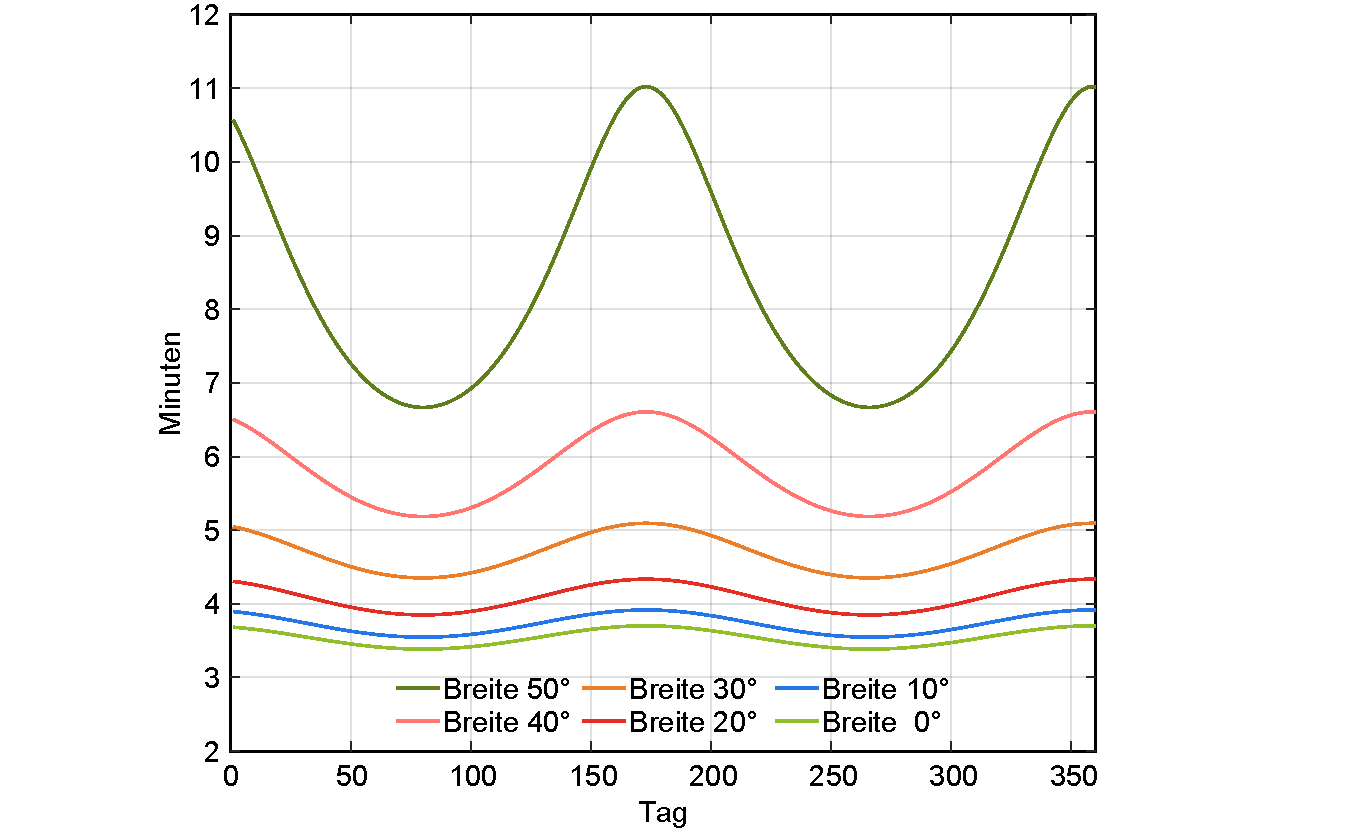
\includegraphics[width=\textwidth]{Tagbogenverlaengerung02.pdf}%
\caption[Tagbogenverl�ngerung durch Refraktion und scheinbaren Radius.]{Tagbogenverl�ngerung durch Refraktion und scheinbaren Radius im Laufe eines Jahres f�r verschiedene geographische Breiten nach \eqref{eq:hm_tagbogverl} (\mscr{} \mlhmref{TagbogenVerlaengerung.m}).}%
\label{abb:hm_tagbogenverl_nach_Delta_tau_A}%
\end{figure}
\figref{hm_tagbogenverl_nach_Delta_tau_A} (\mlhmref{TagbogenVerlaengerung.m}) zeigt sehr deutlich, dass die so berechneten Tagbogenverl�ngerungen bei gro�en geographischen Breiten\index{Breitengrad} und zu den Sonnenwenden am gr��ten sind, was unmittelbar einsichtig ist, wenn man sich die H�he der Sonne im Tagesverlauf f�r verschiedene Jahreszeiten vergegenw�rtigt. In \probref{hm_tageslauf_sonne} werden die H�he der Sonne im Tagesverlauf unter Ber�cksichtigung der Refraktion und der �ber den Tag ver�nderlichen Deklination mittels der Keplerl�sung berechnet und die Abweichung zur N�herung bestimmt.

Damit sind wir nun in der Lage, die Auf- und Untergangszeiten der Sonne in UT vollst�ndig f�r alle geographischen Breiten und Tage des Jahres in der lokalen Ortszeit WOZ anzugeben:
\begin{equation} \label{eq:hm_aufgangszeiten}
t_\text{A,U}(\lambda,\varphi,\delta(t_\text{d})) = 12\!:\!00\:\text{h UT} - \frac{\lambda}{15\degree} + \tau_\text{ ZGL}(\delta) \mp \abs{\tau_\text{ B}}(\varphi,\delta) \mp \abs{\Delta\tau_\text{B}}(\varphi,\delta) \,.
\end{equation}
Hierin ist $\delta\!=\!\delta(t_\text{d})$ als Funktion durch \eqref{eq:hm_delta_von_T_hash} gegeben und damit eine Funktion des bestimmten Tages eines Jahres.
F�r $\tau_\text{ ZGL}(\delta)$ kann im Prinzip jede der verschiedenen Formeln der Zeitgleichung benutzt werden.
\figref{hm_sonne_untergang_baabe} zeigt die nach \eqref{eq:hm_aufgangszeiten} berechneten Zeiten f�r den Sonnenaufgang und Sonnenuntergang, die Kulminationszeiten und die Tagesl�ngen f�r zwei Orte verschiedener geographischer Breiten.
Die Abweichungen zur numerischen L�sung bleiben im Mittel im Bereich von einer Minute. %(siehe dazu auch die \mscre \ref{mls:hm_tagbogenverl} und \ref{mls:hm_tageslauf_sonne}).
\begin{figure}%
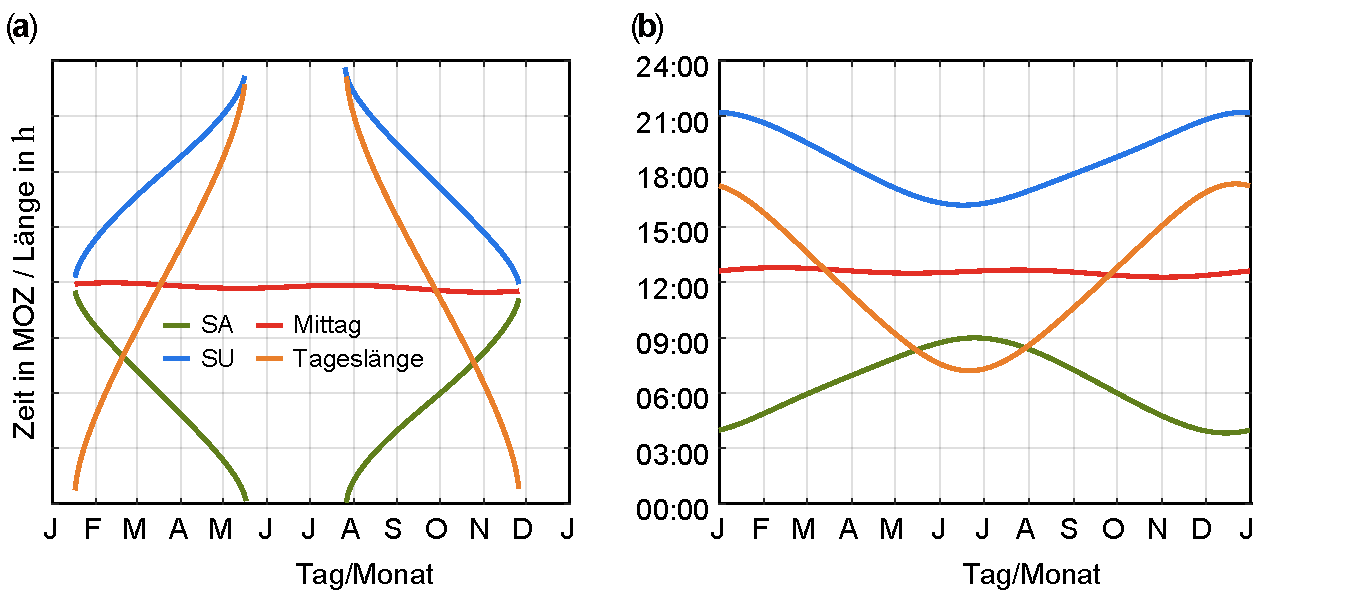
\includegraphics[width=\textwidth]{Sunrise02.pdf}\\%
\caption[Sonnenaufgang und -untergang f�r Troms� und Ushuaia.]{Sonnenaufgang und -untergang f�r \fa Troms�, Norwegen (Breite $69.8\degree$N und L�nge $19.0\degree$E) und \fb Ushuaia, Argentinien (Breite $54.8\degree$S, L�nge $68.3\degree$W). Die $x$-Achsen sind in Monaten angegeben: \anf{J}$=$Januar, \anf{F}$=$Februar, \anf{M}$=$M�rz, \ldots}%
\label{abb:hm_sonne_untergang_baabe}%
\end{figure}

\subparagraph{\textbf{Berechnung des Auf- bzw. Eintauchwinkels der Sonne}}
Zum Schluss wollen wir noch den Auf- \bzw Eintauchwinkel $\vartheta$ der Sonne in den Horizont berechnen.
Der Eintauchwinkel wird eine Funktion der Deklination und geographischen Breite sein.
Der Eintauchwinkel kann nach \figref{hm_verl_tagbogen_ref} wie folgt berechnet werden:
\begin{equation}
\tan\vartheta = \frac{\Delta h}{\Delta \mathcal{A}} \,.
\label{eq:hm_tan_vartheta}
\end{equation}
Unter Benutzung der Kettenregel erhalten wir
\begin{equation*}
\tan\vartheta = \frac{\D h}{\D \mathcal A} = \frac{\D h}{\D \tau}\frac{\D \tau}{\D \mathcal{A}} = \frac{\D h}{\D \tau} \lk \frac{\D \mathcal{A}}{\D \tau} \rk^{-1} \,.
\end{equation*}
Wir bilden die impliziten Ableitungen der Transformationsgleichung f�r $\sin h$ und $\sin \mathcal A$, sodass 
\begin{equation}
\frac{\D h}{\D \tau} = -\cos\delta\cos\varphi\sin\tau ~~\:\text{bzw.} ~~ \:\frac{\D \mathcal{A}}{\D \tau} = \frac{\cos\delta\cos\tau}{\cos\mathcal{A}}\,.
\label{eq:hm_dh_dtau}
\end{equation}
Formel \eqref{eq:hm_dh_dtau} in \eqref{eq:hm_tan_vartheta} eingesetzt ergibt
\begin{equation*}
\tan\vartheta = -\cos\varphi\cos\mathcal{A}_\text{A}\tan\tau_\text{A} \,.
\end{equation*}
Wir benutzen noch einmal die Transformationsformeln f�r $\cos\mathcal{A}$ und $\tan\tau$.
Mit $\cos\mathcal{A}\!=\!-\sin\delta/\cos\varphi$ eingesetzt in $\tan\tau\!=\!-\sin\mathcal{A}/(\tan\varphi\sin\delta)$ erhalten wir schlie�lich 
\begin{equation}
\tan\vartheta = \sqrt{\frac{\cos^2\varphi}{\sin^2\varphi} - \frac{\sin^2\delta}{\sin^2\varphi}} = \sqrt{\frac{\cos^2\delta}{\sin^2\varphi}-1} \,.
\label{eq:hm_tan_vartheta_2}
\end{equation}

\subparagraph{\textbf{Anwendung der Formeln f�r Sonnenauf- und -unterg�nge}}
Wir haben mit der Beziehung \eqref{eq:hm_aufgangszeiten} und mit \eqref{eq:hm_tan_vartheta_2} unser Ziel erreicht und zwei an jedem Ort der Erde und f�r jeden Tag des Jahres g�ltige \anf{Taschenrechnerformeln} erhalten.
W�hrend eines sommerlichen Familien-Ostseeurlaubs 2020 konnten wir die G�ltigkeit obiger Formel wenige Tage vor der Sommersonnenwende in Baabe ($\varphi\!=\!54.3591652\degree,\,\lambda\!=\!13.7061473\degree$) �berpr�fen.\footnote{Die Aufnahme wurde von Sylvia und Michael Kaschke mit einem ZEISS Batis Objektiv mit $\SI{135}{\milli\metre}$ Brennweite und einer Sony Alpha IIC am 10.\,6.\,2020 gemacht!}
Die beobachtete Aufgangszeit um 04:32:20 MESZ stimmt sehr gut mit den Berechnungen �berein (Tabelle \ref{tab:hm_beob_sonnenaufgang_baabe}).
Dies ist insbesondere bemerkenswert, da durch die Temperatur- und Druckvariation in der N�he des Horizonts die H�hen eines Himmelsobjektes um bis zu $0.3$\textdegree\ variieren k�nnen\cite{Meeus1998}.
Deswegen macht es auch keinen Sinn, die Aufgangszeiten wesentlich genauer als auf eine Minute zu berechnen. Unsere N�herungsformeln sind also gut anwendbar.
Signifikante Abweichungen bei diesen ergeben sich erst bei der Anwendung in gr��eren geographischen Breiten.
Generell gilt in der Himmelsmechanik, dass man zum einen mit hoher Genauigkeit (z.\,B. bei den Bahnparametern bzw. der Zeit in JD) rechnen muss, andererseits sollte man ber�cksichtigen, was �berhaupt bis zu welcher Genauigkeit beobachtet werden kann.
Kulminationen sind im Allgemeinen auf wenige Zeitsekunden, Planetenpositionen f�r Amateure auf ca. $10$ bis $20$ Bogensekunden und Aufg�nge wie oben beschrieben auf ca. eine Zeitminute genau beobachtbar.

\begin{table}%
\caption[Beobachtungen und Berechnungen des Sonnenaufgangs in Baabe.]{Beobachtungen und Berechnungen des Sonnenaufgangs in Baabe am 10.6.2020 (alle Zeiten in MESZ).}
\begin{tabular}{L{4cm}L{2.5cm}L{2.5cm}}
\hline\noalign{\smallskip}
  & Astrometrisch & Scheinbar \\
  &(Sonnenzentrum) & (Oberer Rand) \\
\noalign{\smallskip}\svhline\noalign{\smallskip}
JPL\cite{JPL2020} & 04:39:00 & 04:32:00 \\
Berechnet nach \eqref{eq:hm_tau_zgl} & 04:39:35 & 04:32:30 \\
N�herungsformel \eqref{eq:hm_ZGL21} & 04:39:50 & 04:32:10 \\
Beobachtet am 10.\,06.\,2020 & --- & 04:32:40 \\
\noalign{\smallskip}\hline\noalign{\smallskip}
\end{tabular}
\label{tab:hm_beob_sonnenaufgang_baabe}
\end{table}
Auch der Aufgangswinkel $\vartheta$ konnte vermessen werden.
Wenn man in Abb. \ref{eq:hm_sonnenaufgang_baabe_foto} die Anstiege f�r die eingezeichneten Regressionsgeraden bestimmt, so erh�lt man einen Winkel von $\vartheta_1\!=\!25.5$\textdegree\ f�r den oberen Rand der Sonne und $\vartheta_2\!=\!26.8$\textdegree{} f�r den unteren Rand.
Aus einer Rechnung im \mscr~\mlhmref{SonnenaufgangBaabe.m} findet man unter Verwendung der Refraktionsformeln \eqref{eq:hm_Normalrefraktion1} \bzw \eqref{eq:hm_Normalrefraktion2} Werte um $\vartheta\!=\!24.6$\textdegree.
Im Rahmen der Messgenauigkeit stimmt das gut mit unserer Messung �berein.
Aus den unterschiedlichen gemessenen Winkeln wird aber auch deutlich, dass die Refraktion im Bereich $0$\textdegree\ bis $2$\textdegree\ nicht als konstant angenommen werden kann. 
\begin{figure}%
\includegraphics[width=\textwidth]{SunRiseBaabe.pdf}%
\caption[Verlauf des Sonnenaufgangs an der sommerlichen Ostsee.] {Verlauf des Sonnenaufgangs an der sommerlichen Ostsee.}%
\label{eq:hm_sonnenaufgang_baabe_foto}%
\end{figure}
In den \textbf{�bungen} \ref{prob:hm_abflachung_sonne} bis \ref{prob:hm_sonnenaufgang_mars} haben wir einige Beispiele zur Berechnung von Aufgangssituationen auf der Erde bzw. auf einem anderen Planeten vorgesehen.
Die Methodik, die wir bei der Erde verwendet haben, ist auch auf solche F�lle �bertragbar.
In der \probref{hm_analytic_sunrise} wird nach \cite{Reinsch2003} eine Methode dargestellt, mit der eine zumindest f�r die Breitengrade zwischen $25\degree$ und $65\degree$ brauchbare analytische Formel f�r den Sonnenaufgang hergeleitet wird.

\subsubsection{Konstruktion von Sonnenuhren}\index{Sonnenuhr}\label{kap:sonnenuhren}

Mit unserem Wissen �ber die Berechnung der Koordinaten der  Sonne als Funktion und der Zeitgleichung k�nnen wir auch an die Berechnung von Sonnenuhren gehen.
Sonnenuhren sind die �ltesten Zeitmesser auf der Erde.\footnote{In der Literatur wird debattiert, ob Wasser- \bzw Sanduhren noch �lter sind. Diese Uhren k�nnen aber nur Intervalle messen und bestimmen die Zeit nicht in Bezug zur astronomisch definierten Zeit.}
Es gibt ausgezeichnete und umfangreiche Literatur zu diesem Thema \cite{Meyer2008, Kloeckl2017}, weshalb wir uns hier auf die Grundprinzipien beschr�nken und ansonsten auf die Literatur bzw. die �bungen verweisen.

\subparagraph{\textbf{Grundprinzip und Begriffe einer Sonnenuhr}}

Mit einer Sonnenuhr wird durch die Sonne ein (Schatten-)Bild eines Stabes oder eines anderen Objektes auf einem geeignet zu konstruierenden Ziffernblatt erzeugt (\figref{hm_sundial_RvB}).
Aus dem Stand der Sonne bzw. deren Schatten kann dann die Tageszeit (Uhrzeit) unmittelbar abgelesen werden.
Die Tageszeit kann je nach Gestaltung der Sonnenuhr bzw. ihres Zifferblatts als Wahre Ortszeit (WOZ), \gls{moz} (MOZ) oder Zonenzeit (MEZ) angezeigt werden.
Mit Hilfe von Sonnenuhren lassen sich auch jahreszeitliche Informationen ablesen, z.B. das Datum, Sonnenwenden und �quinoktien.
Wir wollen dabei folgende Begriffe aus der \gls{gnomonik} (Lehre von den Sonnenuhren) verwenden (\figref{hm_sundial06}):

\begin{figure}%
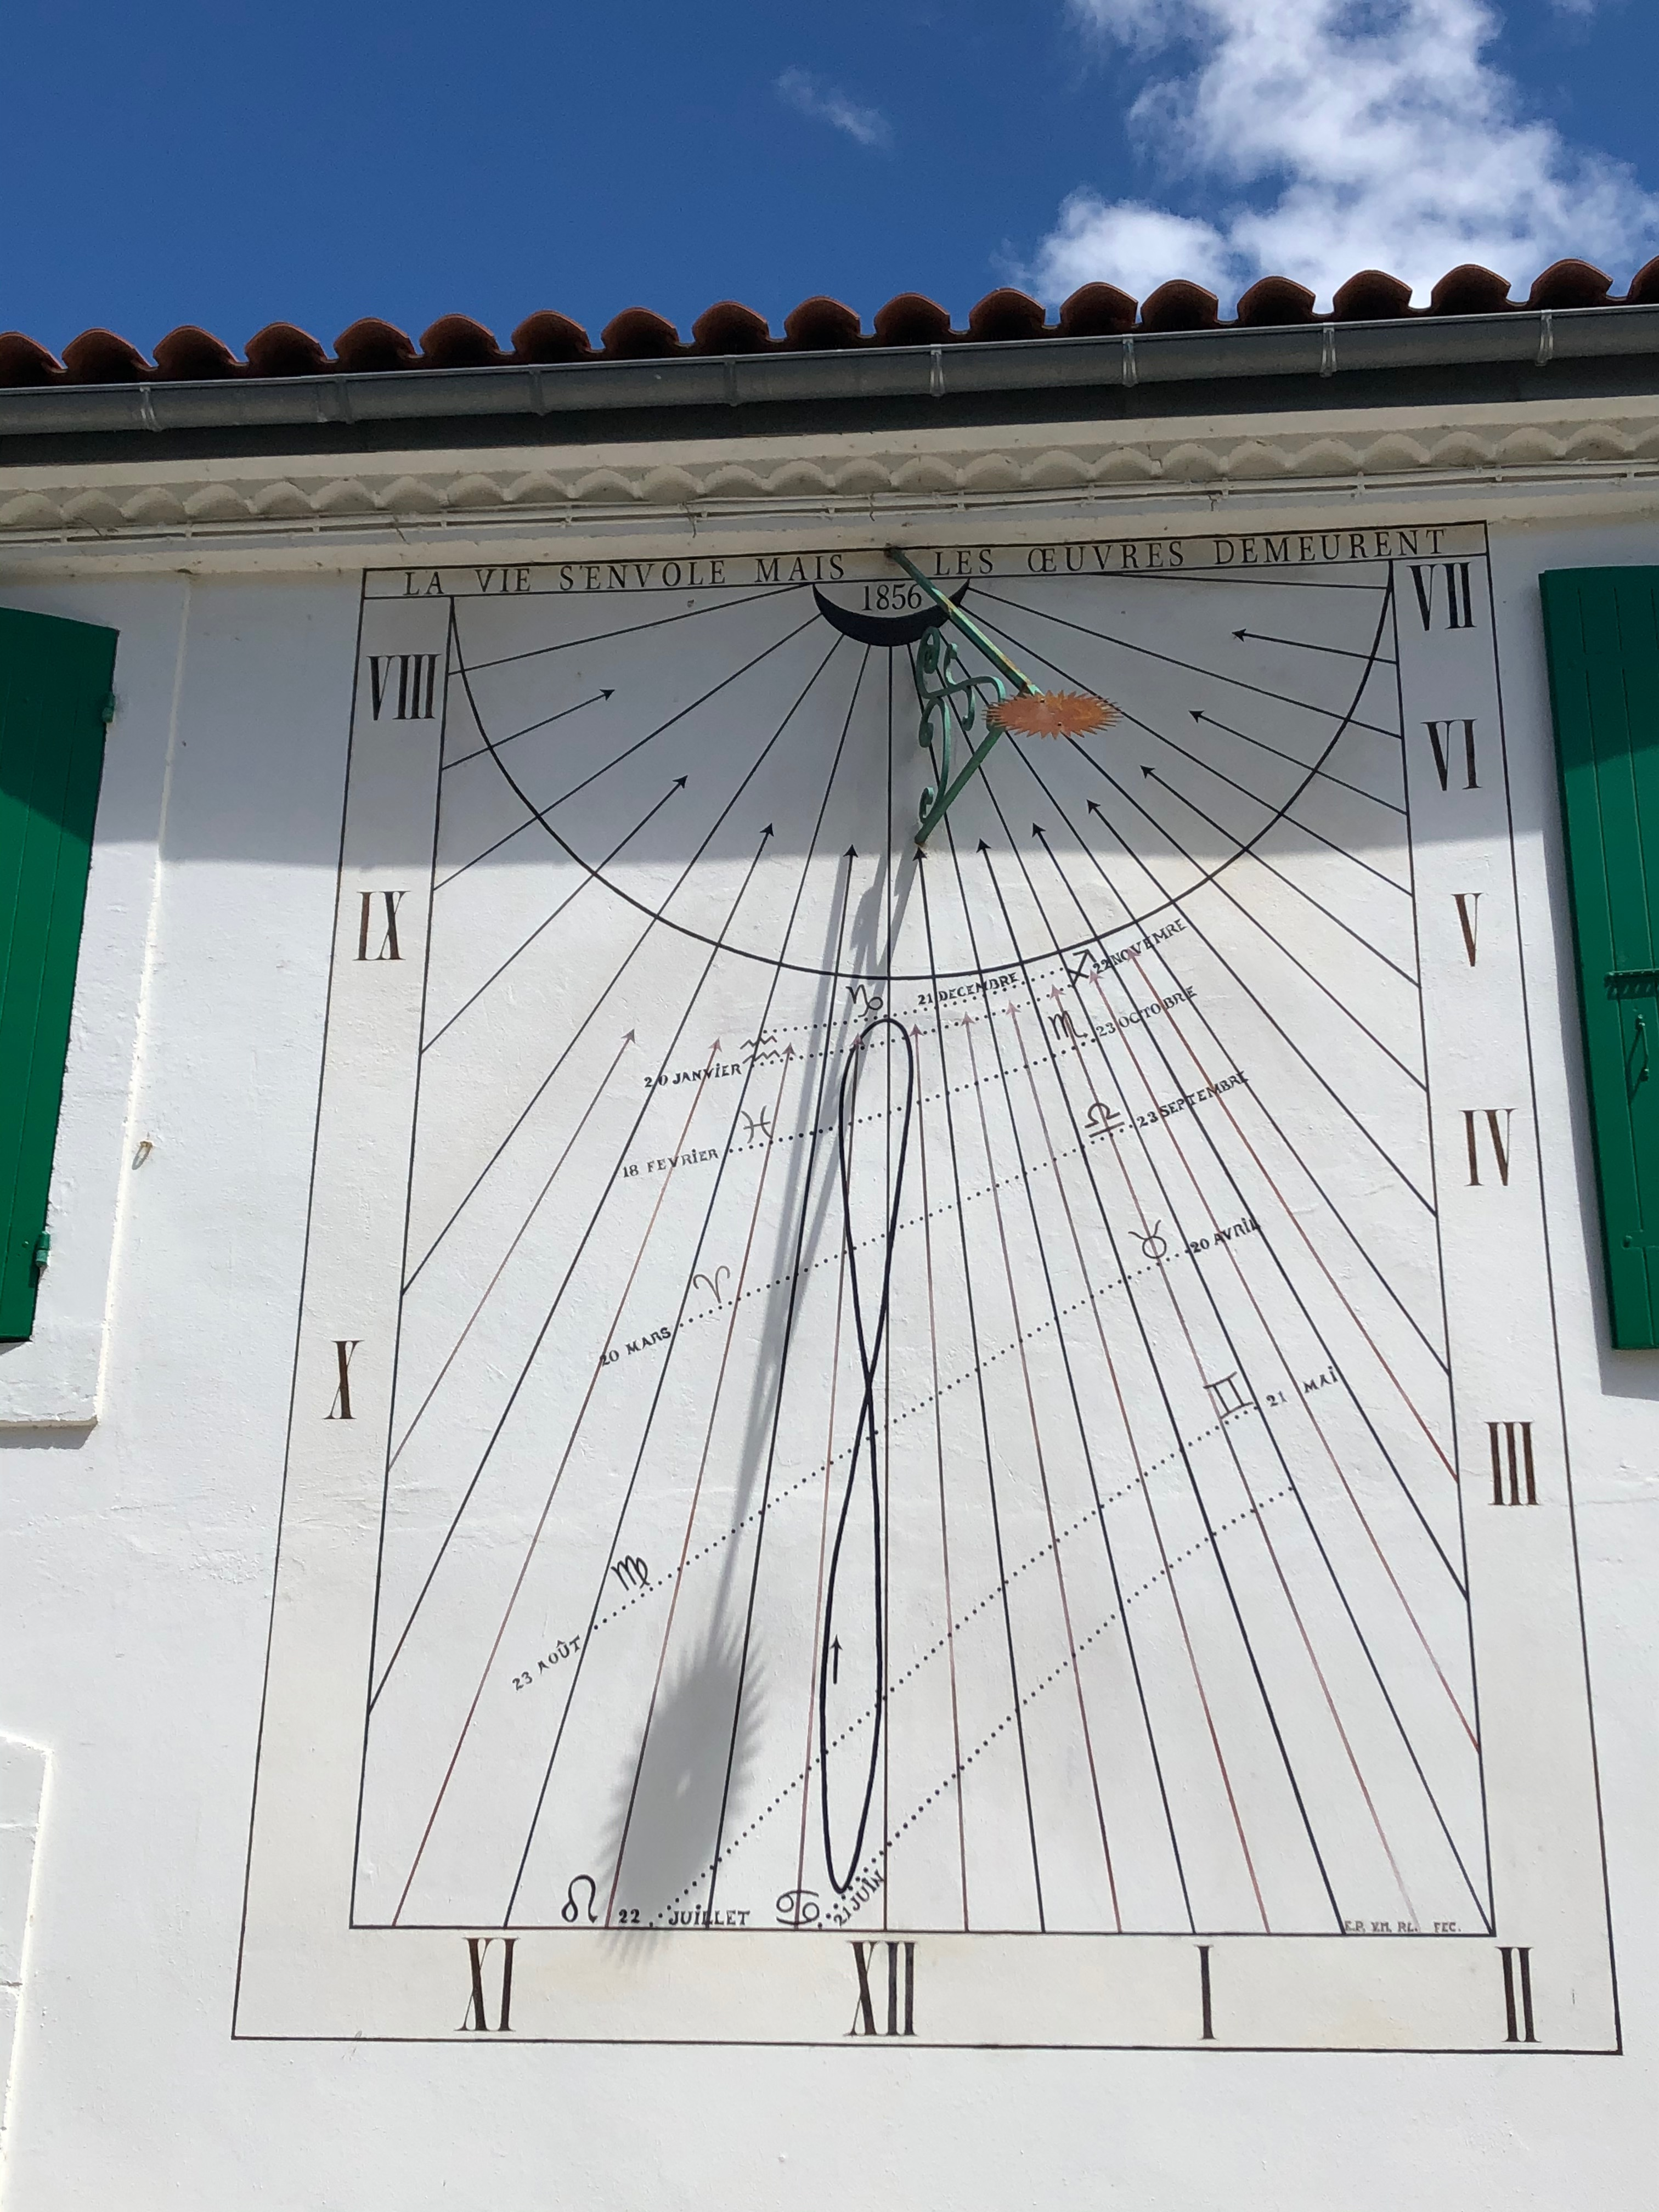
\includegraphics[width=0.4\textwidth]{SunDial.jpg}%
\caption[Sonnenuhr am B�rgermeisteramt in St. Pierre d'Ol�ron in Frankreich.]{Sonnenuhr am B�rgermeisteramt in St. Pierre d'Ol�ron in Frankreich. Die Inschrift auf der Uhr sagt: La vie s'envole, mais les oeuvres demeurent. (Wir bedanken uns bei Rudolf von B�nau f�r das Bild.)}%
\label{abb:hm_sundial_RvB}%
\end{figure}

\renewcommand*{\arraystretch}{1}
\begin{longtable}{L{1.5 cm}L{0.5 cm}L{8.5 cm}}
\noalign{\smallskip}\svhline\noalign{\smallskip}
Begriff & &Erkl�rung \\
\noalign{\smallskip}\svhline\noalign{\smallskip}
\endhead
  \textit{\gls{gnomon}} & & Schattenwerfender Stab.\index{Gnomon}\\ 
  \textit{\gls{nodus}} & & Spitze des Gnomons\index{Nodus} (auch Auge genannt).\\ 
  \textit{\gls{lineatur}} & & Menge der vom Gnomon oder Nodus geworfenen Schatten auf einer Ziffernblattebene\index{Lineatur}, auf der die Zeit abgelesen werden kann.\\
\noalign{\smallskip}\svhline\noalign{\smallskip}
\end{longtable}
\renewcommand*{\arraystretch}{1}

\begin{figure}%
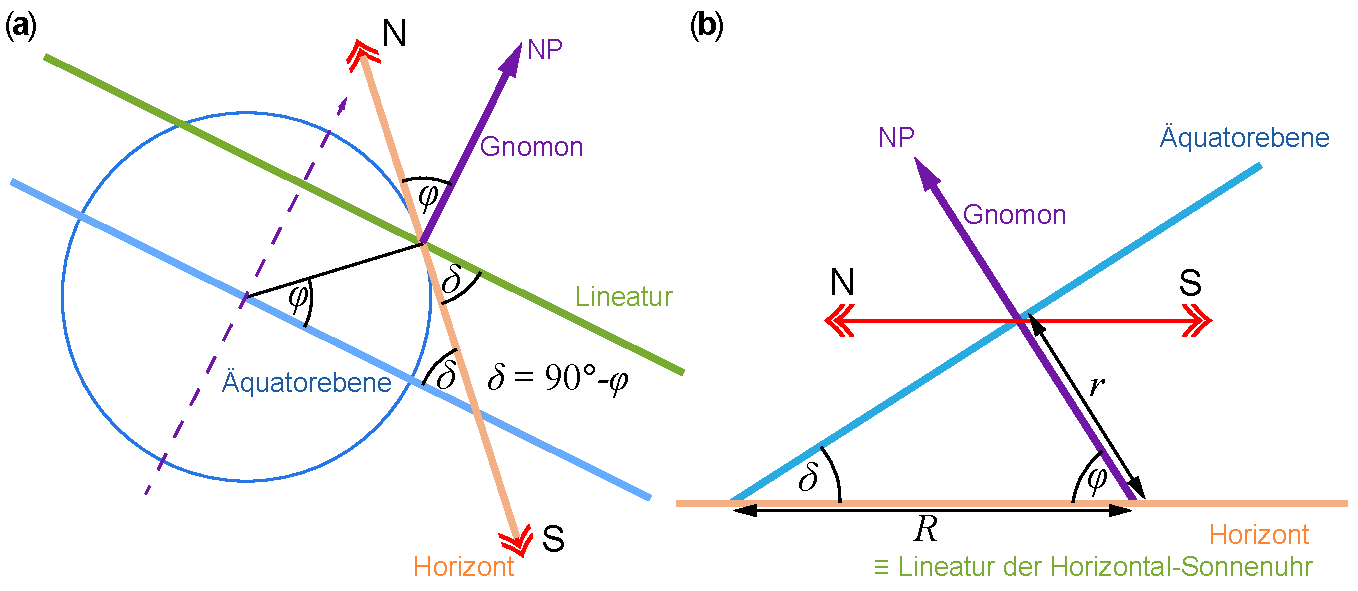
\includegraphics[width=\textwidth]{Sonnenuhr06.pdf}%
\caption[Grundprinzip einer �quatorial- und einer Horizontal-Sonnenuhr.]{Grundprinzip von Sonnenuhren. \fa �quatorial-Sonnenuhr und \fb Horizontal-Sonnenuhr. $\varphi$ ist die geographische Breite, NP der Himmelsnordpol und N, S die Nord- \bzw S�drichtung in der Horizontebene.}%
\label{abb:hm_sundial06}%
\end{figure}

\subparagraph{\textbf{�quatoriale (Polstab-)Sonnenuhr}}

\begin{figure}%
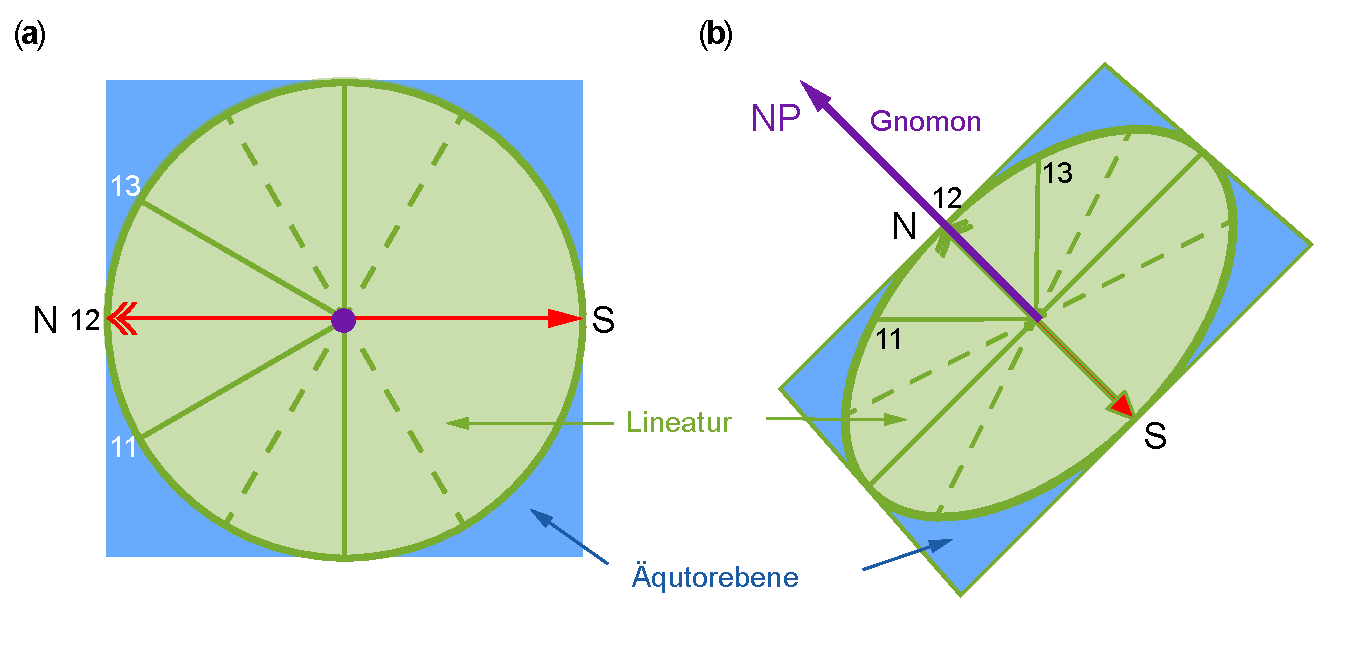
\includegraphics[width=\textwidth]{Sonnenuhr01.pdf}%
\caption[Prinzip und Ausf�hrung einer �quatorial-Sonnenuhr.]{Prinzip und Ausf�hrung einer �quatorial-Sonnenuhr. \fa Draufsicht auf Lineaturebene (parallel zur �quatorebene), \fb Schr�gansicht.}%
\label{abb:hm_sundial01}%
\end{figure}

Diese Sonnenuhr ist die einfachste Sonnenuhr, man findet sie h�ufig in G�rten oder Parks.
Bei ihr liegt das Ziffernblatt mit der Lineatur in einer Ebene, die parallel zur �quatorebene ist.
Die Lineatur ist gleichm��ig aufgeteilt und der Schattenstab steht senkrecht auf dem Ziffernblatt und zeigt damit zum Himmelsnordpol (\figref{hm_sundial02}). \\
Bei positiver Deklination der Sonne kann der Schatten direkt auf dem Ziffernblatt abgelesen werden, bei negativen Deklinationen m�sste das Ziffernblatt transparent sein, da die Sonne von unten den Stab beleuchtet.
Man hilft sich, indem man entweder das Ziffernblatt transparent macht oder als halbkreisf�rmiges Band gestaltet. \\
Die Lineatur ist relativ zur Nordrichtung als Schatten per Definition durch den Stundenwinkel $\tau$ gegeben, den wir im Folgenden mit $\sigma_\text{A}$  bezeichnen wollen. Will man eine Beziehung der Lineatur zur b�rgerlichen Zeit herstellen, so ist unter Annahme einer mittleren Sonne die Lineatur durch

	\begin{align}
				\sigma_\text{A} = \text(MOZ) \frac{15\degree}{\mathrm{h}}+\lambda - \text{Z}\cdot15\degree \label{eq:hm_sundial01}
		\end{align}
gegeben, worin die MOZ wie in \kap{hm_zeitdefinition} definiert die mittlere Ortszeit in Stunden (h), $\lambda$ die geographische L�nge und Z die Zeitzone bedeuten.\\

\subparagraph{\textbf{Horizontal-Sonnenuhr}}

\begin{figure}%
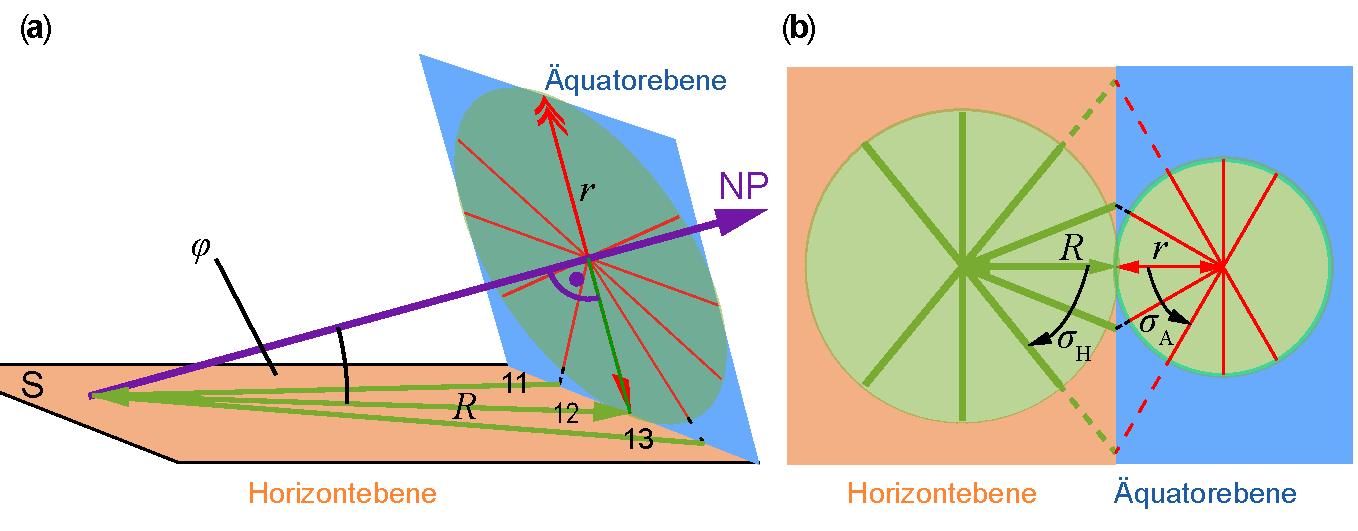
\includegraphics[width=\textwidth]{Sonnenuhr03.pdf}%
\caption[Prinzip der Horizontal-Sonnenuhr.]{\fa Prinzip der Horizontal-Sonnenuhr und \fb Berechnungsgrundlage der Lineatur. $R$ ist hier Radius des Ziffernblatts der Horizontal-Sonnenuhr, $r$ der Radius des Ziffernblatts der �quatorial-Sonnenuhr.}%
\label{abb:hm_sundial02}%
\end{figure}

\begin{figure}%
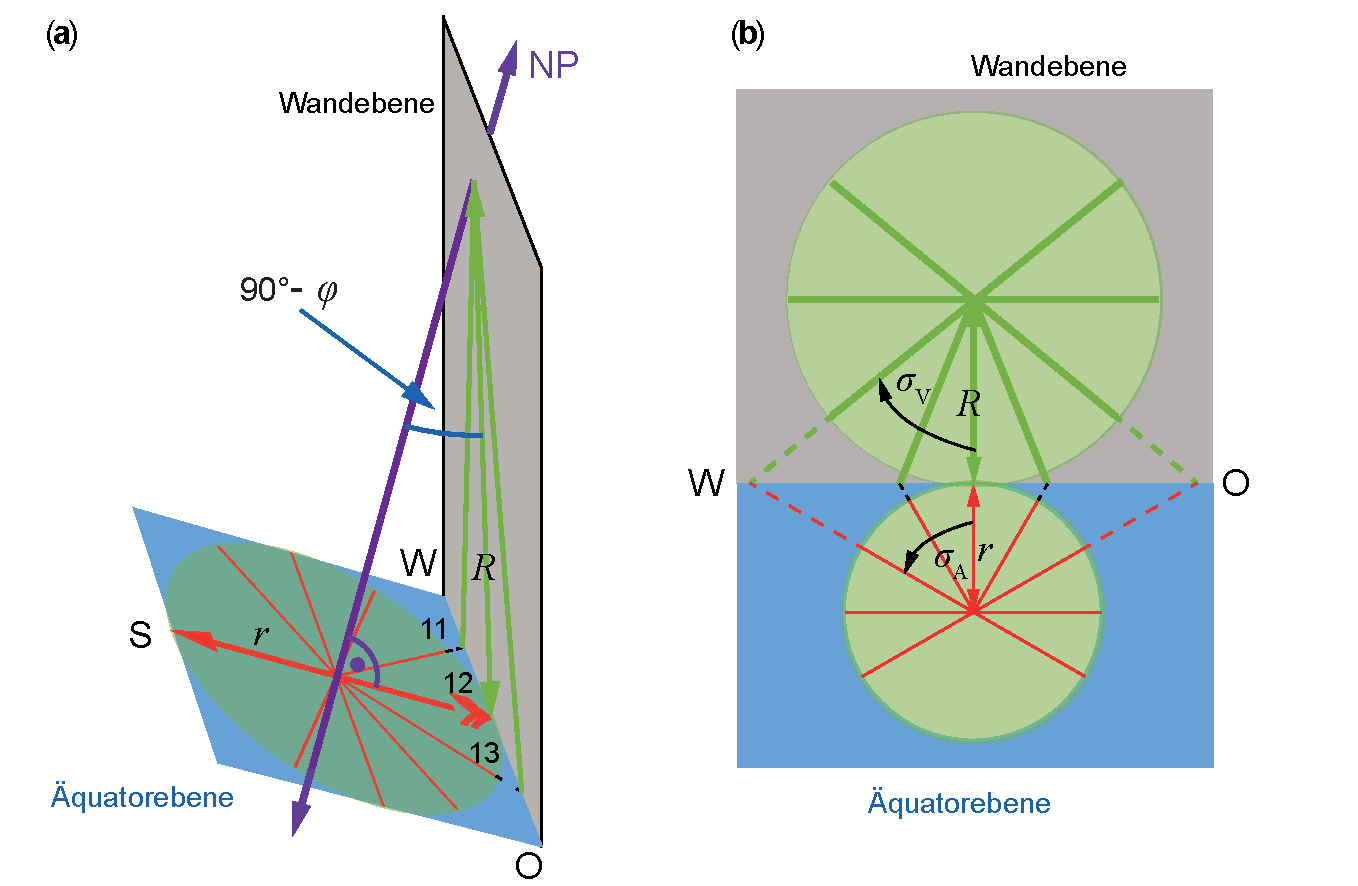
\includegraphics[width=\textwidth]{Sonnenuhr04.pdf}%
\caption[Prinzip der Vertikal-Sonnenuhr.]{\fa Prinzip der Vertikal-Sonnenuhr und \fb Berechnungsgrundlage der Lineatur bei O-W-Ausrichtung der Wand.}%
\label{abb:hm_sundial04}%
\end{figure}

Diese Sonnenuhr findet man auf ebenen Fl�chen, sie sind sehr einfach zu bauen, daf�r ist die Lineatur etwas komplizierter.
Die Konstruktion der Lineatur einer solchen Horizontal-Sonnenuhr ergibt sich aus \figref{hm_sundial02}. \\
Der Schattenstab ist wieder zum Himmelsnordpol ausgerichtet, er bildet also zwischen Horizont- und Ziffernblattebene den Winkel $\varphi$, dessen Gr��e gleich der geographischen Breite des Aufstellungsortes entspricht.
Aus \figref{hm_sundial02} erkennt man, dass die Lineatur nicht mehr gleichm��ig ist.
Sie ergibt sich gem�� einfacher geometrischer �berlegungen zu
		\begin{align}
				\tan \sigma_\text{H} = \frac{r}{R}\,\tan\sigma_\text{A}  = \sin\varphi\,\tan\sigma_\text{A}\,. \label{eq:hm_sundial02}
		\end{align}
$\sigma_\text{H}$ ist hier der Winkel zwischen der Linie f�r die aktuelle Zeit und der 12:00 Stunden-Linie auf dem horizontalen Ziffernblatt, $\sigma_\text{A}$ der entsprechende Winkel auf dem �quatorialen Ziffernblatt.\\
\subparagraph{\textbf{Vertikal-Sonnenuhr}}
Diese Sonnenuhr findet man h�ufig an Hausw�nden.
Ihre Konstruktion ist f�r eine in West-Ost-Richtung verlaufende Wand v�llig analog der Horizontal-Sonnenuhr, nur erfolgt hier die Projektion nicht auf den Horizont, sondern auf eine dazu senkrechte Ebene. Die Uhr stellt quasi eine um $90\degree$ gedrehte Horizontal-Sonnenuhr dar, sodass wir folgende Beziehung erhalten:
		\begin{align}
				\tan\sigma_\text{V}= \sin(90\degree - \varphi)\,\tan\sigma_\text{A} = \cos\varphi\,\tan\sigma_\text{A} \,. \label{eq:hm_sundial03}
		\end{align}
Etwas schwieriger ist die Berechnung, wenn die Wand um einen Winkel $\alpha$  gegen die Ost-West-Achse gedreht ist, was sicher h�ufig vorkommt (\figref{hm_sundial05}). Diese Berechnung wird in \probref{hm_VertikalAnalemmaSonnenuhr} ausgef�hrt. 

\subparagraph{\textbf{Analemmatische Sonnenuhren}}
Bisher haben wir bei der Berechnung der Lineatur die Zeitgleichung nicht ber�cksichtigt, \dh wir haben nach \eqref{eq:hm_sundial01} ein Ziffernblatt f�r die MOZ berechnet.
Da aber die WOZ von der MOZ bis zu $\pm 15 \,\mathrm{min}$ variiert, wollen wir uns eine Sonnenuhr �berlegen, die die ZGL und die unterschiedliche Deklination der Sonne im Laufe eines Jahres ber�cksichtigt. Eine solche Sonnenuhr steht \zb vor dem Galilei-Museum in Florenz (\figref{hm_sundial07}). 

\begin{figure}%
\includegraphics[width=\textwidth]{Sonnenuhr07.pdf}%
\caption[Analemmatische Sonnenuhr vor dem Galilei-Museum in Florenz.]{\fa Analemmatische Sonnenuhr vor dem Galilei-Museum in Florenz (Florenz, Italien) und \fb Konstruktionsprinzip. Nodus (Nd), Nodus-Schattenpunkt (SP), Azimut ($\mathcal{A}$), H�he $H$ des Schattenstabes und H�he $h$ der Sonne (S) sind dargestellt. }%
\label{abb:hm_sundial07}%
\end{figure}

Bei dieser Sonnenuhr erfolgt das Ablesen der Zeit nicht durch eine Schattenlinie, sondern durch den Punktschatten eines Nodus (Nd), der zu jedem Datum einen anderen Punkt des Ziffernblatts beschattet. Der Schattenstab der H�he $H$ muss daher nicht auf den Himmelspol ausgerichtet sein, da es nur auf den Schatten des Nodus ankommt. Wir betrachten die Position $\vec{r}_\text{n}$ des Nodusschattens (SP) in der Horizont-Ziffernblattebene ($x$-$y$-Ebene), wobei $\vec{n}$ die Richtung zum Nodus ist und $\vec{s}$ die Richtung vom Nodus-Schattenpunkt SP zur Sonne S.
Dann gilt (\figref{hm_sundial07}b:
		\begin{align}
				\vec{r}_\text{n} &= \vec{n}+q\,\vec{s} \,, ~~~~ \vec{r}_\text{n}\,\veceZ = 0 = \vec{n}\,\veceZ + q\,\vec{s}\,\veceZ \,, ~~~~~q = -\frac{\vec{n}\,\veceZ}{\vec{s}\,\vec{e}_z} \,, \nonumber \\
				\longrightarrow \vec{r}_\text{n} &= \vec{n}-\frac{\vec{n}\,\veceZ}{\vec{s}\,\veceZ}\vec{s} = \frac{(\vec{s}\,\veceZ)\,\vec{n}-(\vec{n}\,\veceZ)\,\vec{s}}{\vec{s}\,\veceZ} = \frac{\veceZ\times(\vec{n}\times\vec{s})}{\vec{s}\,\veceZ} \,. \label{eq:hm_sundial04}
		\end{align}
Man erkennt aus \eqref{eq:hm_sundial04}, dass die Abbildung der Sonnenrichtung $\vec{s}$ auf das Ziffernblatt nichtlinear ist, da $\vec{s}$ in Z�hler und Nenner steht.
Im Fall der Sonnenuhr von Florenz ist die H�he des Nodusstabes $H \approx \SI{3}{\metre}$.
Im KOS von \figref{hm_sundial07} ergeben sich die Vektoren $\veceZ,\, \vec{n}$ und der Richtungsvektor zur Sonne $\vec{s}$ zu:
	\begin{align*}
                \veceZ&= 
                \begin{pmatrix}
                0 \\
                0 \\
                1
                \end{pmatrix}\,, ~~~~~
                \vec{n}= 
                \begin{pmatrix}
                0 \\
                0 \\
                H
                \end{pmatrix} ~~~~\text{und}~~~~
                \vec{s}= 
                \begin{pmatrix}
                s_\text{x} \\
                s_\text{y} \\
                s_\text{z}
                \end{pmatrix} = 
                \begin{pmatrix}
               	\cos h \, \cos\mathcal{A} \\
               	\cos h \, \sin\mathcal{A} \\
               	\sin h 
								\end{pmatrix}  \,. 
	\end{align*}
Hier haben wir Azimut $\mathcal{A}$ und der H�he $h$ der Sonne verwendet, die man \zb wie in \kap{zeitgleichung} beschrieben zu beliebigen Zeiten $t$ eines Jahres berechnen kann. Die Schattenl�nge und Richtung ergeben sich dann zu (siehe auch \probref{hm_VertikalAnalemmaSonnenuhr}):
		\begin{align}
				\vec{r}_\text{n} = \frac{H}{s_\text{z}(t)}
				\begin{pmatrix}
				-s_\text{x}(t) \\
				-s_\text{y}(t) \\
				0
				\end{pmatrix} = H 
				\begin{pmatrix}
				-\cot\lek h(t)\, \cos\mathcal{A}(t) \rek \\
				-\cot\lek h(t)\, \sin\mathcal{A}(t) \rek \\
				0
				\end{pmatrix}\,. \label{eq:hm_sundial06}
		\end{align}
Man kann mit den Ergebnissen der Rechnung \zb die Linien gleichen Datums (\bzw gleicher Deklination) auftragen und darauf die Uhrzeit markieren.
Alternativ kann man die Stundenlinien (\dh die Punkte f�r eine feste Uhrzeit) im Laufe eines Jahres auftragen.
Dies ist Gegenstand der \probref{hm_VertikalAnalemmaSonnenuhr}.\\
Wir m�chten auch noch auf die relativ einfach und zugleich interessant konstruierte �quatorial-analemmatische Sonnenuhr von Hermann Zeuner \cite{Zeuner2011} verweisen, die in der \probref{hm_Aalener_Sonnenuhr} (Zusatz�bung) n�her betrachtet werden kann.

\subsection{Berechnung von Planetenbahnen}\index{Planetenbahnen}\label{kap:hm_bahnen_hk_ss}

\subsubsection{Berechnung der Planetenbahnen mit Gau�schen Vektoren} \label{kap:hm_bahnen_hk_PQR}
Wir k�nnen nun analog zum Vorgehen in \kapitel{erdbahn} auch Bahnen mit einer Bahnneigung~$i$ zur Ekliptik (\figref{hm_planetenbahnen_rel_ekliptik}) behandeln und damit die Berechnung der Planetenbahnen unseres Sonnensystems in Angriff nehmen.
Dazu m�ssen die Bahnkoordinaten $r$, $\upsilon$, die aus der Kepler-Gleichung berechnet werden, auf die Ekliptik projiziert (\anf{reduziert}) werden.
Diese Projektion ist als eine der Koordinatentransformationen in Tabelle \ref{tab:hm_Umrechung_KOS} gelistet.
Wir wollen hier aber noch einen anderen, sehr eleganten Weg aufzeigen.
Die Abbildung der Vektoren zwischen beiden KOS kann durch eine Matrix-Transformation wie folgt beschrieben werden:
\begin{equation}
\vec{r}_\text{Ekl} = \lk\begin{array}{c} x\\ y\\ z \end{array}\rk = \mathbb{U}\cdot \vec{r}_\text{Bahn} = \lk\begin{array}{ccc} \vec{P} & \vec{Q} & \vec{R} \end{array}\rk \vec{r}_\text{Bahn} = \mathbb{U} \cdot \lk\begin{array}{c} r\cos\upsilon\\ r\sin\upsilon\\ 0 \end{array}\rk ~. \label{eq:hm_gauss_ansatz}
\end{equation}
Die Matrix $\mathbb{U}$ setzt sich aus drei Spalten-Vektoren $\vec{P}$, $\vec{Q}$, $\vec{R}$, den sogenannten Gau�schen\footnote{Johann Carl Friedrich Gau� (auch oft Gauss) (1777 -- 1855) war ein deutscher Mathematiker, Astronom, Geod�t und Physiker. Wegen seiner �berragenden wissenschaftlichen Leistungen galt er bereits zu seinen Lebzeiten als \textit{Princeps mathematicorum - F�rst der Mathematiker}. Seine Arbeiten erstreckten sich von vielen Feldern der Mathematik und Physik auch auf angewandte Gebiete, zum Beispiel der Landesvermessung und der elektromagnetischen Telegraphie.}\indexp{Gau�, Johann Carl Friedrich} Vektoren, zusammen, deren Herleitung im Detail in Beispiel \ref{bsp:herleitung_gauss_vek} beschrieben wird.
Die Gau�schen Vektoren\index{Vektoren!Gau�sche} stellen f�r eine Bahn jeweils Konstanten (f�r das betrachtete �quinoktium) dar, da sie nur von den Bahnparametern abh�ngen:
\begin{align}
\begin{split}
\vec{P} &= \lk\begin{array}{c} + \cos\omega\cos\Omega - \sin\omega\cos i\sin\Omega\\ + \cos\omega\sin\Omega + \sin\omega\cos i\cos\Omega\\ + \sin\omega\sin i \end{array}\rk \,, \\
\vec{Q} &= \lk\begin{array}{c} -\sin\omega\cos\Omega - \cos\omega\cos i\sin\Omega\\ -\sin\omega\sin\Omega + \cos\omega\cos i\cos\Omega\\ + \cos\omega\sin i \end{array}\rk \,, \\
\vec{R} &= \lk\begin{array}{c} + \sin i\sin\Omega\\ -\sin i\cos\Omega\\ + \cos i \end{array}\rk \,. 
\end{split} \label{eq:hm_gauss_vektoren}
\end{align}
Der Vorteil ist offensichtlich.
Wenn man die zeitliche Entwicklung der Bahnkoordinaten berechnet hat, braucht man f�r die Projektion auf die Ekliptik die Matrix $\mathbb{U}$ nur einmal auszurechnen.
Diese Methodik ist dann sehr effizient, wenn man viele Koordinaten �ber viele St�tzstellen berechnen muss oder die Geschwindigkeiten des Himmelsk�rpers braucht.

%BEISPIEL 5 %%%%%%%%%%%%%%%%%%%%%%%%%%%%%%%%%%%%%%%%%%%%%%%%%%%%%%%%%%%%%%%%%%%%%%%%%%%%%%%%%%
\begin{example}{\textbf{\textit{Herleitung der Gau�schen Vektoren}}}
Wir wollen die Gau�schen Vektoren nach \eqref{eq:hm_gauss_vektoren} herleiten.
Wir starten dabei von den kartesischen Koordinaten der Bahnebene und wollen daraus die heliozentrischen kartesischen Koordinaten herleiten.
Dazu benutzen wir f�r die Transformation zwischen den beiden KOS die Drehmatrizen mit den entsprechenden Bahnparametern.
\medskip\\
Die gesamte Transformation kann man als Abfolge dreier Rotationen betrachten:
\begin{enumerate}[(1)]
	\item \emph{Drehung in der Bahnebene um die $z$-Achse zur Ber�cksichtigung der Perihellage $\omega$ relativ zum aufsteigenden Knoten}\\
	Der Ausgangsvektor ist gegeben als
	\begin{align*}
	\vec{r}_0 = \lk\begin{matrix} r \cos \upsilon \\ r \sin \upsilon \\ 0 \end{matrix} \rk\,.
\end{align*}
	Nach der Drehung um $-\omega$ zeigt die neue $x$-Achse in Richtung des Knotens.
        Die Drehung wird beschrieben durch 
	\begin{align*}
	\vec{r}_1\:=\:\mathbb{R}_z(-\omega)\, \vec{r}_0 = 
	\lk\begin{matrix} +\cos \omega &\; -\sin \omega &\; 0 \\
	                     +\sin \omega &\; +\cos \omega &\; 0 \\
                          0         &\;     0        &\; 1 \end{matrix} \rk \cdot \vec{r}_0 \ \:=\: 
													r \lk\begin{matrix} \cos u \\ \sin u \\ 0 \end{matrix} \rk 
\end{align*}
mit $u\!=\!\upsilon+\omega$.
	\item \emph{Drehung der Bahnebene um die $x$-Achse in die Ekliptikebene zur Korrektur der Bahnneigung $i$ gegen�ber der Ekliptik}
\begin{align*}
	\vec{r}_2\:=\:\mathbb{R}_x(-i)\cdot \vec{r}_1 =
	\lk\begin{matrix} 1 &\; 0 &\; 0 \\ 0 &\; +\cos i &\; -\sin i \\ 0 &\; +\sin i &\; +\cos i \end{matrix} \rk \cdot \vec{r}_1 \ =
	r \lk\begin{matrix} \cos u \\ \sin u \cos i\\ \sin u \sin i \end{matrix} \rk ~\,.
\end{align*}
	\item \emph{Drehung um die $z$-Achse in der Ekliptikebene zur Ber�cksichtigung der Knotenlage $\Omega$ relativ zum Fr�hlingspunkt} $\vernal$
	\begin{align*}
	\vec{r}_3 = \mathbb{R}_z(-\Omega)\cdot \vec{r}_2 &=
	\lk\begin{matrix} +\cos \Omega &\; -\sin \Omega &\; 0 \\
	                     +\sin \Omega &\; +\cos \Omega &\; 0 \\
                          0         &\;     0        &\; 1 \end{matrix} \rk\cdot \vec{r}_2 \\
        &= r\,\lk\begin{matrix} \cos u \cos \Omega - \sin u \cos i \sin \Omega \\ \cos u \sin \Omega - \sin u \cos i \cos \Omega \\ \sin u \sin i \end{matrix} \rk \,.
\end{align*}
\end{enumerate}
Man kann die Gesamttransformation nat�rlich auch mit einer Matrix $\mathbb{U} (-\omega,-i,-\Omega)\!=\! \mathbb{R}_z(-\Omega) \mathbb{R}_x(-i) \mathbb{R}_z(-\omega)$ beschreiben.
Durch Ausmultiplizieren findet man
\begin{align*}
\mathbb{U} = \lk
\begin{matrix}
       + \cos\omega\cos\Omega - \sin\omega\cos i\sin\Omega &\; -\sin\omega\cos\Omega - \cos\omega\cos i\sin\Omega &\; + \sin i\sin\Omega \\
       + \cos\omega\sin\Omega + \sin\omega\cos i\cos\Omega &\; -\sin\omega\sin\Omega + \cos\omega\cos i\cos\Omega &\;- \sin i\cos\Omega \\
			 + \sin\omega\sin i                                  &\; + \cos\omega\sin i                                 &\; + \cos i \end {matrix} \rk \,.
\end{align*}
Die Spalten dieser Matrix $\mathbb{U}$ entsprechen nun genau den Gau�schen Vektoren $\vec{P},\,\vec{Q},\,\vec{R}$ in \eqref{eq:hm_gauss_vektoren}.
Man kann leicht zeigen, dass die Gau�schen Vektoren Einheitsvektoren sind.
Diese Einheitsvektoren spannen ein sogenanntes \textit{kartesisch-perifokales Koordinatensystem}\index{Koordinatensystem!perifokales} auf. 
Dieses ist dadurch definiert, dass dessen Ursprung weiterhin im Nullpunkt des Zentralk�rpers (z.\,B.\, der Sonne $\astrosun$) liegt und dessen $x,y$-Ebene die Bahnebene des durch die Bahnparameter gegebenen Himmelsk�rpers ist \cite{Walter2018}.
Der Vektor $\vec{R}$ zeigt dann logischerweise in Richtung des Drehimpulses  $\vec{L}$ und der Vektor $\vec{P}$ in Richtung des Laplace-Vektors $\vec{e}$. \\ 
\end{example}
%BEISPIEL %%%%%%%%%%%%%%%%%%%%%%%%%%%%%%%%%%%%%%%%%%%%%%%%%%%%%%%%%%%%%%%%%%%%%%%%%%%%%%%%%%
Dem aufmerksamen Leser wird nicht entgangen sein, dass die hier eingef�hrten Winkel eine gro�e �hnlichkeit mit den Euler-Winkeln\index{Euler-Winkel} aus Kapitel 1.4.2.2 (Band I) haben, die wir beim starren K�rper eingef�hrt haben, ja diesen auf  Grund der Bildungsvorschrift sogar entsprechen. Wir empfehlen dem Leser nachzuvollziehen, dass folgende �quivalenzen gelten:
\begin{longtable}{p{0.33\textwidth}p{0.05\textwidth}p{0.33\textwidth}}
\hline\noalign{\smallskip}
Starrer K�rper & &Himmelsmechanik \\
Euler-Winkel & &Bahnparameter \\
\hline\noalign{\smallskip}
$\varphi$ & &$\omega$ \\
$\vartheta$ & &$i$\\
$\psi$ & &$\Omega$
%\noalign{\smallskip}\hline\noalign{\smallskip}
\end{longtable} \label{bsp:herleitung_gauss_vek}
\medskip

In den \mscren \mlhmref{InnerePlaneten.m} \bzw \mlhmref{AeusserePlaneten.m} sind die Rechnungen f�r die inneren und �u�eren Planeten ausgef�hrt (Ergebnisse in \figref{hm_proj_bahnen_innere_pl} und \figref{hm_bahnen_aussere_pl}).
Aus der Berechnung der Bahnen f�r die �u�eren Planeten f�r den Zeitraum 1920--2020 k�nnen wir auch sehen, dass es Jahre gab, in denen selbst zu Zeiten, als Pluto noch ein \anf{vollwertiger} Planet war, Neptun wegen der Exzentrizit�t der Pluto-Bahn der am weitesten von der Sonne entfernte Planet war.

Wegen der wechselseitigen St�rungen der �u�eren Planeten ist es streng genommen eigentlich nicht m�glich, ihre Bahnen durch (mittlere) Bahnparameter zu beschreiben.\\
Die Rechnungen nach \mlhmref{AeusserePlaneten.m} k�nnen daher nur als grobe N�herungen betrachtet werden und sind nur auf ca. ein Grad genau.\footnote{F�r die Behandlung von St�rungen der einfachen Keplerbahn durch andere Himmelsk�rper verweisen wir auf die einf�hrende Diskussion der St�rungsrechnung im \kap{stoerungsrechnung} und auf weiterf�hrende Literatur \cite{Murray2008,Brouwer1961,Guthmann2000}.}

\begin{figure}%
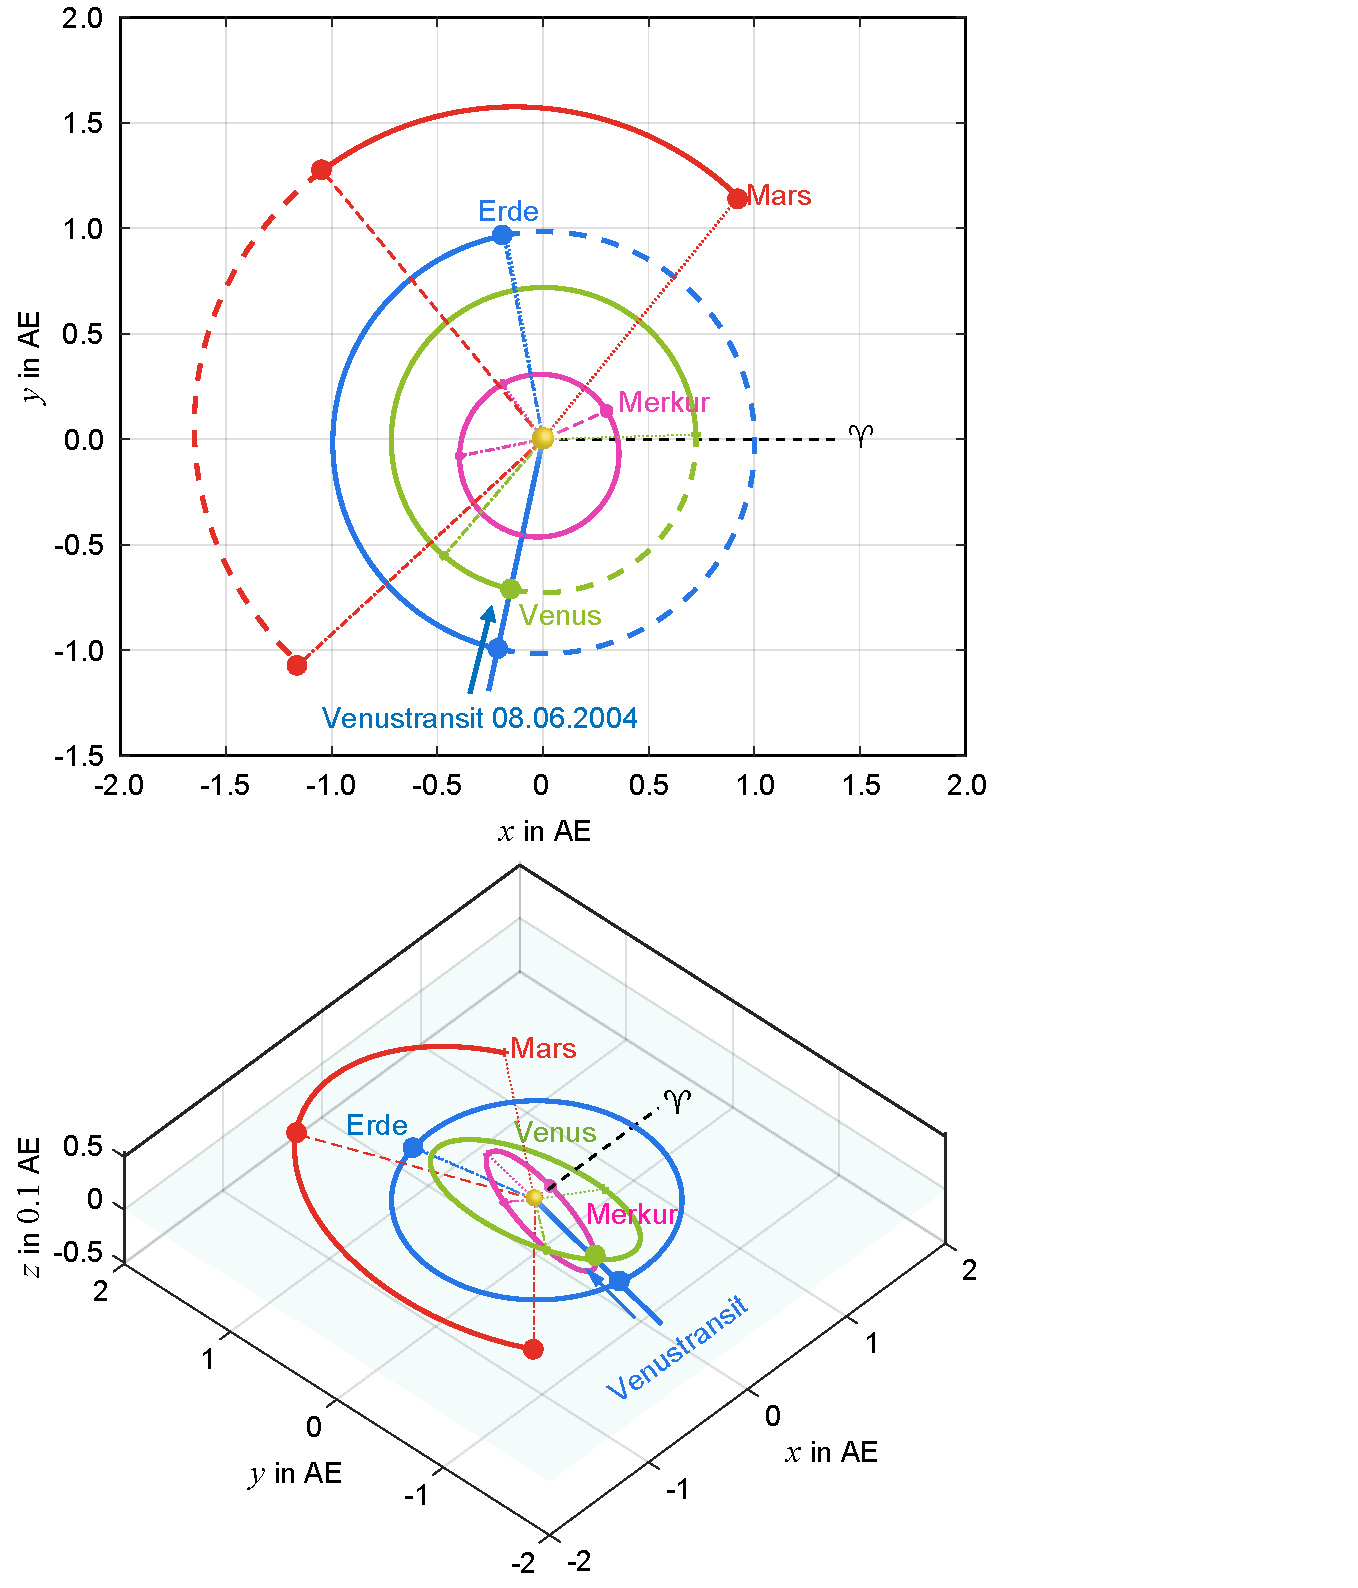
\includegraphics[width=\textwidth]{InnerePlaneten.pdf}\\%
\caption[Projektion der Bahnen der inneren Planeten auf die Ekliptik.]{Projektion der Bahnen der inneren Planeten auf die Ekliptik f�r das Jahr 2004 in Draufsicht (oben) und 3D-Darstellung (unten). Die Bahnen sind unterschiedlich f�r die Zeitr�ume 01.\,01.\,2004 bis 07.\,06.\,2004 (durchgezogen) und 08.\,06.\,2004 bis 31.\,12.\,2004 (gestrichelt) gezeichnet. F�r den 08.\,06.\,2004 erkennt man einen Venustransit\index{Venustransit}, das ist ein Durchgang der Venus vor der Sonnenscheibe, wie er von der Erde aus beobachtet werden konnte (dicke blaue durchgezogene Linie).}%
\label{abb:hm_proj_bahnen_innere_pl}%
\end{figure}

\begin{figure}%
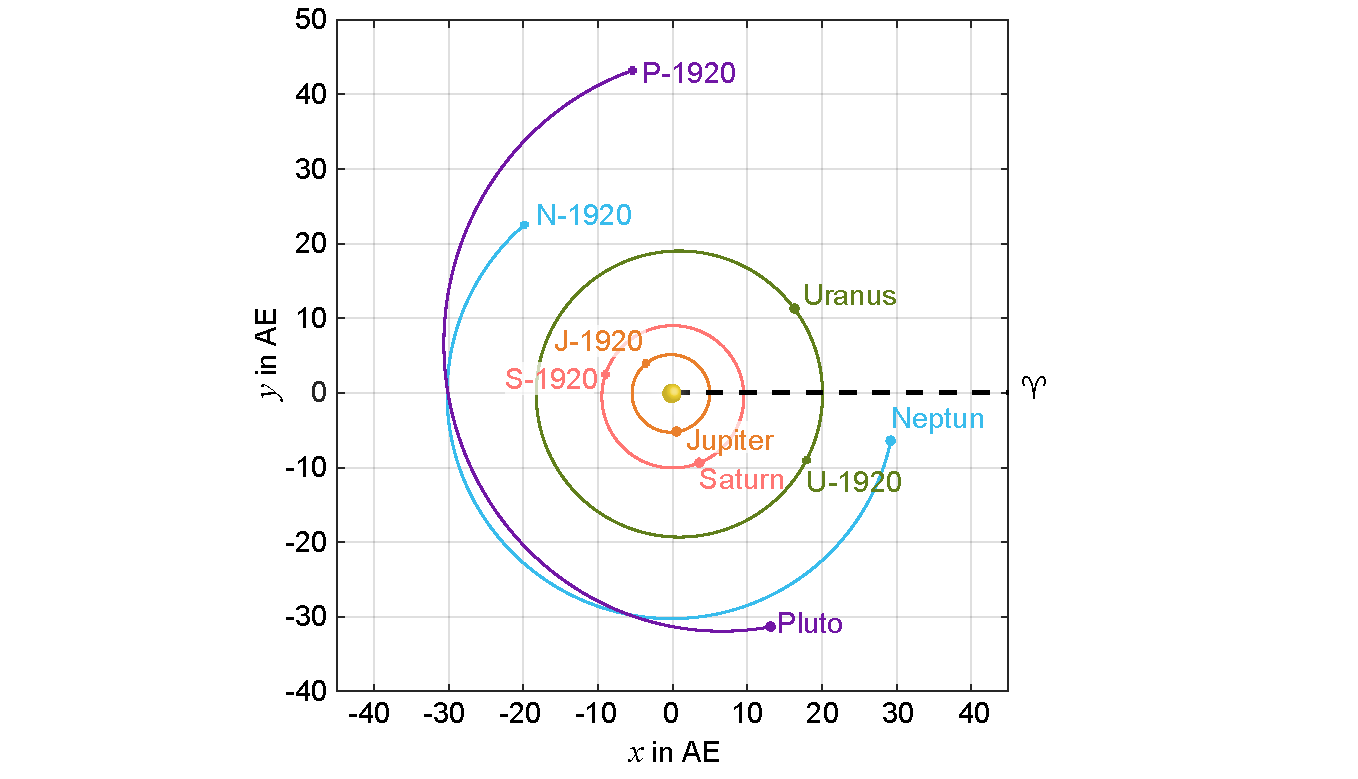
\includegraphics[width=\textwidth]{AeusserePlaneten.pdf}%
\caption{Bahnen der �u�eren Planeten im Zeitraum von 1920 bis 2020.}%
\label{abb:hm_bahnen_aussere_pl}%
\end{figure}

\subsubsection{N�herungsformel f�r die Berechnung der Bahnen von Planeten -- Reduktion auf die Ekliptik}\label{kap:reduktion_ekliptik}\index{Reduktion!auf die Ekliptik}
Bei Planeten ist im Gegensatz zu den sp�ter behandelten Kometen die Neigung der Bahn $i$ gegen die Ekliptik im Allgemeinen relativ klein.
Deshalb kann man eine N�herungsformel f�r die Berechnung der ekliptikalen Koordinaten aus den Bahnkoordinaten herleiten.
Die Herleitung dieser sogenannten Reduktionsformel\index{Reduktionsformel} ist in Beispiel \ref{bsp:herleitung_redformel_ekl} im Detail ausgef�hrt.
Man startet bei \figref{hm_planetenbahnen_rel_ekliptik} und benutzt die aus der sph�rischen Trigonometrie bekannte Beziehung (siehe auch die \onlineZ)
\begin{equation}
\tan(l-\Omega) = \cos\epsilon\tan(\upsilon+\omega)~. \label{eq:hm_reduktions_formel1}
\end{equation}

Die sogenannte Reduktion\index{Reduktion} $\mathcal{R}$ ist definiert als Differenz von ekliptikaler L�nge und wahrer Anomalie (abz�glich des konstanten Wertes $\varpi$ der L�nge des Perihels):
\begin{equation}
\mathcal{R} = l-(\upsilon+\varpi) \label{eq:hm_reduktions_formel2} ~.\\
\end{equation}

Wir geben hier das Resultat f�r $\mathcal{R}$ an und verweisen auf die detaillierte Rechnung in Bsp. \ref{bsp:herleitung_redformel_ekl}:
\begin{equation}
\mathcal{R} = -\tan^2\lk\frac{i}{2}\rk \sin\lek 2(M+\omega) \rek + \frac{1}{2} \lek \tan^2\lk\frac{i}{2}\rk\rek^2 \sin\lek 4(M+\omega) \rek - \ldots  ~.\label{eq:hm_reduktions_formel3}\\
\end{equation}
Aus \eqref{eq:hm_reduktions_formel2} folgt mit der Beziehung $l(t)\!\approx\!\upsilon(t) + \varpi + \mathcal{R}(t)\!\approx\!\mathcal{C}(t)+M(t)+\varpi + \mathcal{R}(t)$ die ekliptikale L�nge $l$ als Funktion der mittleren Anomalie $M$\glslink{mittlereanom}:
\begin{align}
\begin{split}
l(M) =& M + \varpi + 2e\sin M + \lek \frac{5}{4} e^2 - \tan^2\lk\frac{i}{2}\rk \cos(2\omega) \rek \sin(2M) \\ 
      &+ \lek -\tan^2\lk\frac{i}{2}\rk \sin(2\omega)\rek \cos(2M) + \ldots\,. 
\end{split} \label{eq:hm_reduktions_formel4} 
\end{align}
In �hnlicher Weise lassen sich Berechnungsformeln f�r die ekliptikale Breite $b$ und den Abstand $r$ gewinnen:
\begin{align}
b(M(t)) =& -ie\sin\omega + i\sin\omega\cos M + i\cos\omega\sin M \label{eq:hm_reduktions_formel5} \\ 
      & +ie\sin\omega\cos(2M) + ie\cos\omega\sin(2M) +\ldots\nonumber \\ \nonumber\\
r(M(t)) =& a\lk 1+\frac{e^2}{2} \rk - ae\cos M - a \frac{e^2}{2} \cos(2M) +\ldots\,. \label{eq:hm_reduktions_formel6} 
\end{align}
Diese elegante und einfach programmierbare Berechnung der ekliptikalen Koordinaten ist als N�herung f�r viele Anwendungsf�lle, insbesondere f�r Planeten mit geringer Bahnneigung, gut geeignet.
In den \textbf{�bungen} \ref{prob:hm_opposition_mars}, \ref{prob:hm_erdaufgang_von_mond} und \ref{prob:hm_erdaufgang_von_apollo} sind einige Anwendungsbeispiele f�r die Berechnung von Planeten- und Mondbahnen ausgef�hrt.\\
  
%BEISPIEL 6 %%%%%%%%%%%%%%%%%%%%%%%%%%%%%%%%%%%%%%%%%%%%%%%%%%%%%%%%%%%%%%%%%%%%%%%%%%%%%%%%%%
\begin{example}{Herleitung der Reduktionsformel auf die Ekliptik\index{Reduktion!auf die Ekliptik}}
\itshape Wir wollen die Reduktionsformel \eqref{eq:hm_reduktions_formel3} herleiten und starten dazu von \figref{hm_planetenbahnen_rel_ekliptik}.
Wir benutzen dabei vorteilhafterweise die Formeln, die wir bei der Herleitung der Mittelpunktsgleichung in \probref{hm_alternative_MPG} erhalten haben.\\
\upshape
In \figref{hm_planetenbahnen_rel_ekliptik} gilt im sph�rischen Dreieck PKE$_\text{P}$ nach der sph�rischen Trigonometrie
\begin{equation*}
\cos i = \frac{\tan \overline{\text{KE}}_\text{P}}{\tan \overline{\text{KP}}} = \frac{\tan(l-\Omega)}{\tan(\upsilon+\omega)} = \frac{\tan\Theta}{\tan u} \,,
\end{equation*}
worin $\upsilon$ wieder die wahre Anomalie ist und $l$ die ekliptikale L�nge, also
\begin{equation*}
\tan\Theta = \cos i \tan u \,.
\end{equation*}
Wir dr�cken nun $\cos i$ durch den Tangens des halben Winkels aus und erhalten
\begin{equation*}
\tan\Theta = \frac{1-\tan^2\lk\frac{i}{2}\rk}{1+\tan^2\lk\frac{i}{2}\rk} \tan u \equiv \frac{1-y}{1+y} \tan u \,.
\end{equation*}
Diese Gleichung haben wir in gleicher Struktur in \probref{hm_alternative_MPG} ausgewertet und sind dort auf die folgende Form gekommen:
\begin{align*}
\upsilon &= E + 2 \lk x\sin E + \frac{x^2}{2}\sin 2E + \frac{x^3}{3}\sin 3E + \ldots \rk ~.
\end{align*}
Hier ist $x\!=\!-y$, $\upsilon \!=\! 2 \Theta$ und $E\!=\!2u$ zu setzen, woraus folgt:
\begin{align*}
\Theta &= u- y\sin 2u + \frac{y^2}{2}\sin 4u - \frac{y^3}{3}\sin 6u + \ldots \,.
\end{align*}
Wir setzen jetzt wieder $\Theta\!=\!l-\Omega$ und $u\!=\!\upsilon+\omega$ und k�nnen schreiben:
\begin{align*}
l - (\Omega  + \omega) &= l - \varpi \\
&= \upsilon - y\sin\lk 2(\upsilon+\omega)\rk + \frac{y^2}{2}\sin\lk 4(\upsilon+\omega)\rk + \ldots ~.
\end{align*}
F�r die meisten Planeten ist $i\!<\!10\degree$, sodass $y\!=\!\tan^2(i/2)$ eine kleine Gr��e ist und wir Terme mit $y^2$ und h�her vernachl�ssigen k�nnen.
Wir setzen jetzt f�r $\upsilon$ die Mittelpunktsgleichung \eqref{eq:hm_mpglg_nu-M} mit $\upsilon\!=\! M + \mathcal{C} = M + 2e\sin M + \frac{5e^2}{4}\sin(2M) +  \ldots$ ein und erhalten
\begin{align*}
l & \approx \! \varpi + \underbrace{M + 2e\sin M + \frac{5e^2}{4}\sin(2M)}_{\upsilon = M + \mathcal{C}} \\ 
&- y\lek \sin(2(\upsilon)) \cos(2\omega) + \cos(2(\upsilon)) \sin(2\omega)\rek + \ldots ~.
\end{align*}
Wir k�nnen f�r kleine $e$ in den Winkelfunktionen $\upsilon \approx M$ setzen und erhalten schlie�lich
\begin{align}
\begin{split}
l &\approx \! \varpi + M + 2e\sin M + \lek \frac{5e^2}{4} - \tan^2\lk\frac{i}{2}\rk \cos(2\omega) \rek \sin(2M) \\
& - \lek \tan^2\lk\frac{i}{2}\rk \sin(2\omega) \rek \cos(2M) + \mathcal{O}\lk e^3,\tan^4\lk\frac{i}{2}\rk \rk\,,
\end{split} \label{eq:hm_reduktions_formel_Bsp}
\end{align}
was Gleichung \eqref{eq:hm_reduktions_formel4} entspricht.\\
Vergleicht man die Geometrie von \figref{hm_planetenbahnen_rel_ekliptik}, f�r die wir die Reduktionsformel abgeleitet haben, mit der Geometrie von \figref{hm_wahre_sonne_geoz}, erkennt man, dass wir die Reduktionsformel auch in diesem Fall, der sogenannten Reduktion auf den �quator\index{Reduktion!auf den �quator}, anwenden k�nnen.
Wir m�ssen dann nur folgende Substitution vornehmen: $l\!\rightarrow\!\lambda $ und $\upsilon + \varpi\!\rightarrow\!\alpha$. \\

\label{bsp:herleitung_redformel_ekl}
\end{example}
%BEISPIEL %%%%%%%%%%%%%%%%%%%%%%%%%%%%%%%%%%%%%%%%%%%%%%%%%%%%%%%%%%%%%%%%%%%%%%%%%%%%%%%%%%

\subsubsection{Venustransit}\index{Venustransit} \label{kap:hm_veustransit}

In \figref{hm_proj_bahnen_innere_pl} haben wir gesehen, dass am 08.\,06.\,2004 Erde, Venus und Sonne in einer Linie \anf{lagen}.
Unter Ber�cksichtigung des scheinbaren Durchmessers der Sonne von \ca $30'$ ergibt unsere Rechnung, dass zumindest prinzipiell (abh�ngig von der genauen topozentrischen Position) ein Beobachter auf der Erde einen Venustransit beobachten kann, \dh er kann sehen, wie sich die Venus vor die Sonne bewegt
(Tab.~\ref{tab:hm_venustransit}).
Tats�chlich war f�r viele Beobachter in Mitteleuropa das Wettergl�ck auf ihrer Seite und der Transit sehr sch�n zu beobachten (\figref{hm_venustransit}).
Venustransits geh�ren zu den seltensten der exakt vorhersagbaren astronomischen Ereignisse.
Kein im Jahre 2004 lebender Mensch hatte zuvor einen solchen Transit beobachten k�nnen, weil im gesamten vergangenen 20.\ Jahrhundert kein einziger stattfand.
Der n�chste Transit wird erst wieder im Jahre 2117 zu verfolgen sein.
Seit dem Aufkommen des Teleskops konnten �berhaupt nur sieben Venustransits von Menschen beobachtet werden (1639, 1761, 1769, 1874, 1882, 2004, 2012). 

\begin{figure}%
\includegraphics[width=\textwidth]{VenustransitKombi.pdf}%
\caption[Venustransit 2004.]{\fa Venustransit 2004 (Private Aufnahme um 06:40 UT in 48.8�N/10.7�O) und \fb Berechnung mit den \mscr en \mlhmref{VenusTransit01.m} und \mlhmref{VenusTransit02.m}.}%
\label{abb:hm_venustransit}%
\end{figure}

Unserer Rechnungen mit den \mscr en \mlhmref{VenusTransit01.m} \bzw \mlhmref{VenusTransit02.m} ergeben relativ genaue Ergebnisse, weichen jedoch geringf�gig von den Daten des \textit{\gls{jplhm}~(JPL)}\index{Jet Propulsion Lab (JPL)} \cite{JPL2020} ab.%
\footnote{Mit unserem \mscr{} findet man noch mit guter Genauigkeit einen weiteren Transit der Venus f�r den 06.\,06.\,2012.} Dies erkl�rt sich, wenn man bedenkt, dass wir
\begin{itemize}
	\item reine Keplerbahnen angenommen haben, \dh den Einfluss der anderen Planeten und vor allem des Mondes auf die Erdbahn vernachl�ssigt haben,
	\item die Pr�zession der Erdachse in unserer Rechnung nicht ber�cksichtigt haben.
\end{itemize}
Die Ber�cksichtigung dieser Effekte ist Gegenstand der St�rungstheorie, deren Grundidee wir in \kap{stoerungsrechnung} vorstellen wollen. 

\begin{table}%
\caption[Koordinaten von Erde, Venus und Sonne am 08.06.2004 um 08:00 und 12:00 UT.]{Koordinaten von Erde, Venus und Sonne am 08.06.2004 um 08:00 und 12:00 UT. Die Rektaszension $\alpha$ ist wie �blich in \text{hh}$^\text{h} \text{mm}^\text{m} \text{ss}^\text{s}$ angegeben.}
\begin{adjustbox}{width=\textwidth,totalheight=\textheight,keepaspectratio}
\begin{tabular}{l|c|cc|cc|cc}
\hline\noalign{\smallskip}
 - & UT & \multicolumn{2}{c|}{Sonne} & \multicolumn{2}{c|}{Venus} & \multicolumn{2}{c}{Erde} \\
\noalign{\smallskip}\svhline\noalign{\smallskip}
Heliozentrisch & & & & $l$ & $b$ & $l$ & $b$ \\
\noalign{\smallskip}\svhline\noalign{\smallskip}
\multirow{2}{*}{JPL \cite{JPL2020}} & 08:00 &  &  & $257.7883\degree$ & $-0.0665\degree$ & $257.8015\degree$ & $0.0007\degree$ \\
                                    & 12:00 &  &  & $258.0527\degree$ & $-0.0822\degree$ & $257.9609\degree$ & $0.0007\degree$\\
\hline\noalign{\smallskip}		
\multirow{2}{*}{\mlhmref{InnerePlaneten.m}} 
																	& 08:00 &  &  & $257.7885\degree$ & $-0.0662\degree$ & $257.8015\degree$ & $-0.0005\degree$ \\
																	& 12:00 &  &  & $258.0529\degree$ & $-0.0813\degree$ & $257.9837\degree$ & $-0.0005\degree$ \\
\noalign{\smallskip}\svhline\noalign{\smallskip}
Geozentrisch & & $\lambda$ & $\beta$ & $\lambda$ & $\beta$ &  &  \\
\noalign{\smallskip}\svhline\noalign{\smallskip}
\multirow{2}{*}{JPL \cite{JPL2020}} & 08:00 & $77.8605\degree$ & $-0.0002\degree$ & $77.9079\degree$ & $-0.1691\degree$ &  &  \\
                                    & 12:00 & $78.0199\degree$ & $-0.0002\degree$ & $77.8031\degree$ & $-0.2086\degree$ &  &  \\
\hline\noalign{\smallskip}		
\multirow{2}{*}{\mlhmref{InnerePlaneten.m}} 
                                  & 08:00 & $77.8243\degree$ & $0.0005\degree$ & $77.9143\degree$ & $-0.1630\degree$ &  &  \\
																	& 12:00 & $77.9837\degree$ & $0.0005\degree$ & $77.8097\degree$ & $-0.2025\degree$ &  &   \\		
\noalign{\smallskip}\svhline\noalign{\smallskip}
�quatorial & & $\alpha$ & $\delta$ & $\alpha$ & $\delta$ &  &  \\
\noalign{\smallskip}\svhline\noalign{\smallskip}
JPL \cite{JPL2020} 
	& 08:00 & $05^\text{h}06^\text{m}51^\text{s}$ & $22\degree52'46''$ & $05^\text{h}07^\text{m}16^\text{s}$ & $22\degree42'55''$ &  &  \\
	& 12:00 & $05^\text{h}07^\text{m}41^\text{s}$ & $22\degree53'38''$ & $05^\text{h}06^\text{m}50^\text{s}$ & $22\degree40'00''$ &  &  \\
\hline\noalign{\smallskip}		
\mlhmref{InnerePlaneten.m}
	& 08:00 & $05^\text{h}07^\text{m}04^\text{s}$ & $22\degree52'54''$ & $05^\text{h}07^\text{m}31^\text{s}$ & $22\degree43'37''$ &  &  \\
	& 12:00 & $05^\text{h}07^\text{m}45^\text{s}$ & $22\degree53'46''$ & $05^\text{h}07^\text{m}05^\text{s}$ & $22\degree40'42''$ &  &  \\
\noalign{\smallskip}\hline\noalign{\smallskip}
\end{tabular}
\end{adjustbox}
\label{tab:hm_venustransit}
\end{table}

\begin{figure}
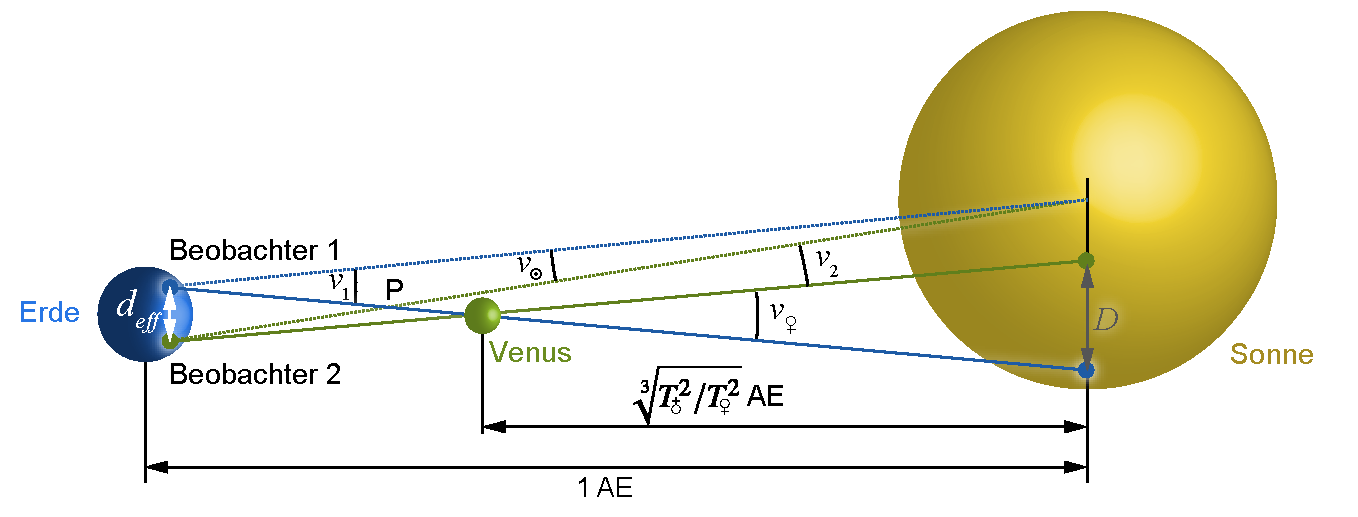
\includegraphics[width=\textwidth]{VenusParallax_exakt.pdf}%
\caption[Messung der Venus-Parallaxe f�r zwei Beobachter auf der Erde.]{Messung der Venus-Parallaxe f�r zwei Beobachter auf der Erde (allgemeiner Fall, nach \cite{Backhaus2020}).}%
\label{abb:hm_VenusParallax}%
\end{figure}

Venustransits sind auch wissenschaftshistorisch sehr interessant.
Die gleichzeitige Beobachtung des Transits von verschiedenen Orten der Erde aus erlaubte erstmalig die genaue Bestimmung des Abstandes zwischen Sonne und Erde, \dh der Astronomischen Einheit\index{Astronomischen Einheit} (AE)\glslink{ae}.
Hierbei nutzte man aus, dass die Position der Venus relativ zur Sonnenscheibe im Prinzip gut messbar ist (\figref{hm_VenusParallax}).
Deshalb machte Halley\indexp{Halley, Edmund}\footnote{Edmund Halley (1656--1742) war k�niglicher Astronom und Leiter der Sternwarte in Greenwich, Mathematiker, Kartograph, und Meteorologe. Neben seinen Berechnungen von Kometenbahnen erforschte Halley auch den Erdmagnetismus, den Monsun, die Eigenbewegung von Sternen und berechnete die \index{H�henformel!barometrische} \glslink{baroHoeheHm}{barometrische H�henformel}.} bereits 1716 den Vorschlag, beim (f�r ihn) n�chsten Venustransit 1761 (den er nicht mehr erlebte) von verschiedenen Orten der Erde (effektiver Abstand $d_\text{eff}$) aus die Parallaxe $\nu_\text{1,2}$ der Venus auf der Sonnenscheibe gleichzeitig zu vermessen (\figref{hm_VenusParallax}).
Um daraus die Sonnenentfernung so genau wie m�glich bestimmen zu k�nnen, muss die Entfernung Sonne-Venus auf die Entfernung Erde-Sonne nach dem 3.~Keplerschen Gesetz $a_\text{\earth}\!=\!a_\text{\venus}\,\sqrt[3]{T_\text{\earth}^2/T_\text{\venus}^2} $ hochgerechnet werden, woraus sich dann mit $\Delta\nu = \nu_\text{1} -\nu_\text{2}$ die astronomische Einheit bestimmen l�sst zu
\begin{equation}
1 \text{AE} = a_\text{\earth} =\frac{d_\text{eff}}{\lk \frac{a_\text{\earth}}{a_\text{\venus}} - 1 \rk \Delta\nu}\,.\label{eq:hm_Venus_AE_Messung}
\end{equation}
Die Entfernung zwischen Erde und Sonne ist die Grundlage f�r die Bestimmung der Gr��e des Sonnensystems und damit auch f�r die Messung der astrophysikalischen Eigenschaften (wie Massen, Dichten) von Planeten und Sternen.
Bis zum 17. Jahrhundert existierten nur vage Vorstellungen �ber die Gr��enordnung dieser Entfernung und die Bestimmung dieser Gr��e galt f�r viele Jahrhunderte als eines der Hauptprobleme der Astronomie.
Deshalb war es auch nicht ganz verwunderlich, dass 1761 (und auch 1769) auf Basis von Halleys Vorschlag mit viel Geld eine ganze Reihe von Expeditionen �ber Monate in entlegenste Gebiete geschickt wurden -- wobei einige dann am Tag des Venustransits einen bew�lkten Himmel oder defekte Instrumente vorfanden.\footnote{Eine sehr sch�ne und spannende Darstellung dieses ersten gro�en internationalen Wissenschaftsabenteuers findet man in \cite{Wolf2017}.
Eine ebenfalls lesenswerte und kurz zusammengefasste Geschichte der Bestimmung der AE findet sich in \cite{Hudson2004}.} Heute in Zeiten des Internets ist das nat�rlich viel einfacher realisierbar \cite{Backhaus2014}.
Wir empfehlen dazu Beispiel \ref{bsp:venustransit} und \probref{hm_venus_2004_2012} durchzuarbeiten, in denen wir konkret die Vorgehensweise zur Bestimmung der Astronomischen Einheit nachvollziehen.

%BEISPIEL 7 %%%%%%%%%%%%%%%%%%%%%%%%%%%%%%%%%%%%%%%%%%%%%%%%%%%%%%%%%%%%%%%%%%%%%%%%%%%%%%%%%%

\begin{example}{Venustransit und Bestimmung der AE}
\begin{enumerate}[(a)]
  \item Wir wollen zeigen, wie aus der gleichzeitigen fotografischen Beobachtung des Venustransits an zwei verschiedenen Positionen auf der Erde mit bekannten Koordinaten die Astronomische Einheit bestimmt werden kann (siehe \figref{hm_VenusTransit2012}).
    Wir wollen dazu Daten einer solchen Beobachtung, die man im Internet \zb unter \cite{Venustransit2012} finden kann, benutzen.\\
\begin{center}
	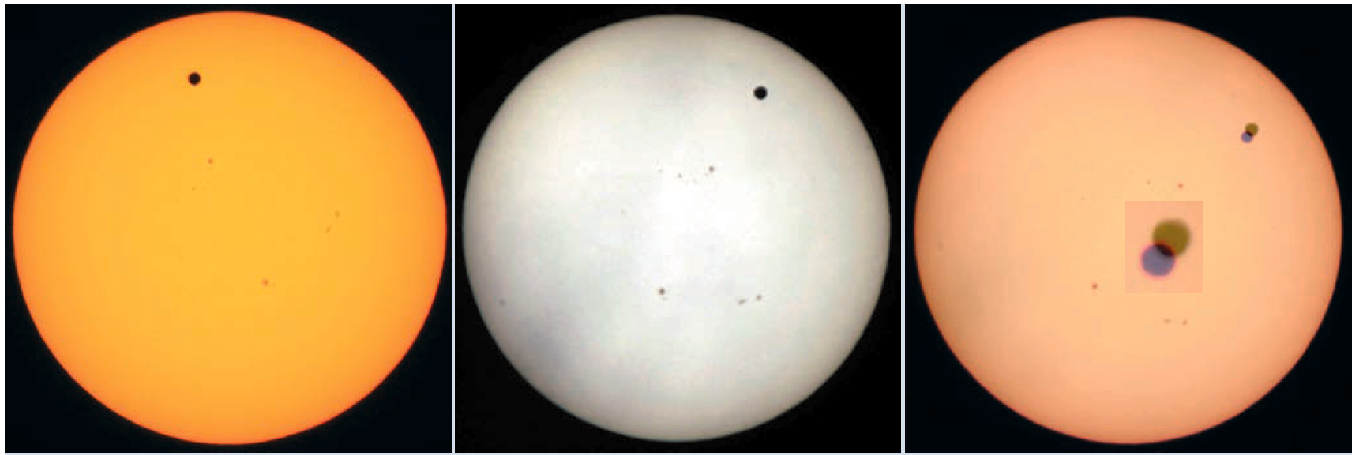
\includegraphics[width=0.9\textwidth]{VenusTransit2012.pdf} 
\captionof{figure}[Venustransit 2012.]{Venustransit 2012. Zeitgleiche Aufnahmen des Transits aus Troms� (links) und Canberra (Mitte) \cite{Venustransit2012}. Im rechten Bild sind die beiden Bilder mit der gleichen Ausrichtung der Sonnenachse �berlagert. (Man benutzt dazu z.B. die Position der Sonnenflecken). Im rechten Bild ist in der Mitte zur Verdeutlichung eine Vergr��erung des Winkelunterschiedes der in den beiden Standorten sich unterscheidenden Venusprojektionen zu sehen.}\label{abb:hm_VenusTransit2012}
\end{center}

Man kann aus dem Bild durch Ausmessen den Winkelunterschied f�r die beiden Projektionen zu $\Delta\nu \approx 0.021 \, b_\text{w\astrosun}$ bestimmen, worin $b_\text{w\astrosun} = 0.5317\degree$ der Bildwinkel der Sonne ist, unter dem sie von der Erde aus erscheint.
        Den effektiven Abstand zwischen Troms� und Canberra berechnet man zu $d_\text{eff} = 11415 \:\text{km}$ (\probref{hm_venus_2004_2012}).
        Aus \eqref{eq:hm_Venus_AE_Messung} ergibt sich dann mit den Werten $	T_\text{\venus} = 224.701 \:\text{d}, T_\text{\earth} = 365.256 \:\text{d}$:
\begin{align*}
	\gamma \!&= \!\frac{a_\text{\earth}}{a_\text{\venus}}=\sqrt[3]{\frac{T_\text{\earth}^2}{T_\text{\venus}^2}}= 1.382~~\text{und daraus}\\ 
\rightarrow a_\text{\earth} \!&=\:\!152.6\: \text{Mio km}
\end{align*}

Dieser Wert stimmt relativ gut mit dem exakten Wert �berein.
Ungenauigkeiten resultieren vor allem aus der Bestimmung von $\Delta\nu$ aus den Fotografien.
	\item Man kann die Bestimmung der Astronomischen Einheit auch durch einen einzigen Beobachter an einem festen Ort der Erde realisieren.
          Bei der zeitlichen Verfolgung des Venustransits nutzt man die durch die Erdrotation entstehende Parallaxe aus.
          Man muss dann die sogenannten Kontaktzeiten bestimmen, z.\,B. die Zeit $T_\text{II}$ bzw. $T_\text{III}$, wenn der Rand der Venusprojektion den Rand der \anf{Sonnenscheibe} von innen ber�hrt.
          Alternativ bestimmt man die Transitzeit $T_\text{TR}$, die sich die Venusprojektion vom Ort des Beobachters betrachtet auf der Sonnenscheibe befindet.
          Diese Transitzeit betr�gt einige Stunden und muss sehr genau ermittelt werden, was hohe Anforderungen an die Messung stellt.
          Wir wollen die Genauigkeit der Kontaktzeitmethode\index{Kontaktzeitmethode} mit der Genauigkeit der Parallaxenmethode\index{Parallaxe} an zwei Beobachtungsorten vergleichen \cite{Rempel2019} und nehmen dabei zun�chst f�r eine erste Absch�tzung vereinfachend an, dass die Planeten Erde und Venus sich auf kreisf�rmigen Bahnen in der Ekliptikebene um die Sonne bewegen.\\
	Wir betrachten dazu in \figref{hm_VenusTransitd}
        den Fall (a).
        F�r die L�nge der Projektion auf der Sonne gilt
	\begin{align*}
		\frac{\D s_\text{\venus}-\D s_\text{\earth}}{a_\text{\earth}-a_\text{\venus}}&=\frac{\D P_\text{B} - \D s_\text{\earth}}{a_\text{\earth}}~.
		\end{align*}
		Mit den Beziehungen f�r die Winkelgeschwindigkeiten $\D s_i\!=\!\omega_i a_i \D t$, $\D P_\text{B}\!=\!\Omega_\text{B} a_\text{\earth} \D t$ und $\gamma\!=\! a_\text{\earth}/a_\text{\venus}$ erhalten wir
	\begin{align*}
\Omega_\text{B} = \frac{1}{a_\text{\earth}} \frac{\D P_\text{B}}{\D t}= \frac{\omega_\text{\venus} - \omega_\text{\earth} }{\gamma-1} ~.
	\end{align*}
$\Omega_\text{B}$ ist die Winkelgeschwindigkeit des Projektionspunktes auf der Sonnenscheibe.
Wir nehmen weiter an, dass der Venustransit durch den Sonnenmittelpunkt verlaufe.
Dann ist die maximal m�gliche Transitzeit gegeben durch
\begin{equation*}
T_\text{TR,max} = \frac{b_\text{w\astrosun}}{\Omega_\text{B}}=28500 \:\text{s} \approx \:7\:\text{h}\:54\:\text{min} \,.
\end{equation*}	
Wie wir in \figref{hm_venustransit} sehen, erfolgt der Transit aber entlang einer Sehne mit der relativen L�nge $l_\text{S\astrosun}$.
Wir k�nnen diese L�nge wiederum gut im Verh�ltnis zu $b_\text{w\astrosun}$ aus den fotografischen Aufnahmen zu $\approx 0.78$ bestimmen, woraus sich eine Transitzeit $T_\text{TR,B}$ in guter N�herung ergibt zu
\begin{equation*}
T_\text{TR}= \frac{l_\text{S\astrosun} \, b_\text{w\astrosun}}{\Omega_\text{B}} = 22230\:\text{s} \approx \:6\:\text{h}\:11\:\text{min} \,.
\end{equation*}	
Das entspr�che der Transitzeit f�r einen Beobachter im Erdmittelpunkt.

\begin{center}
	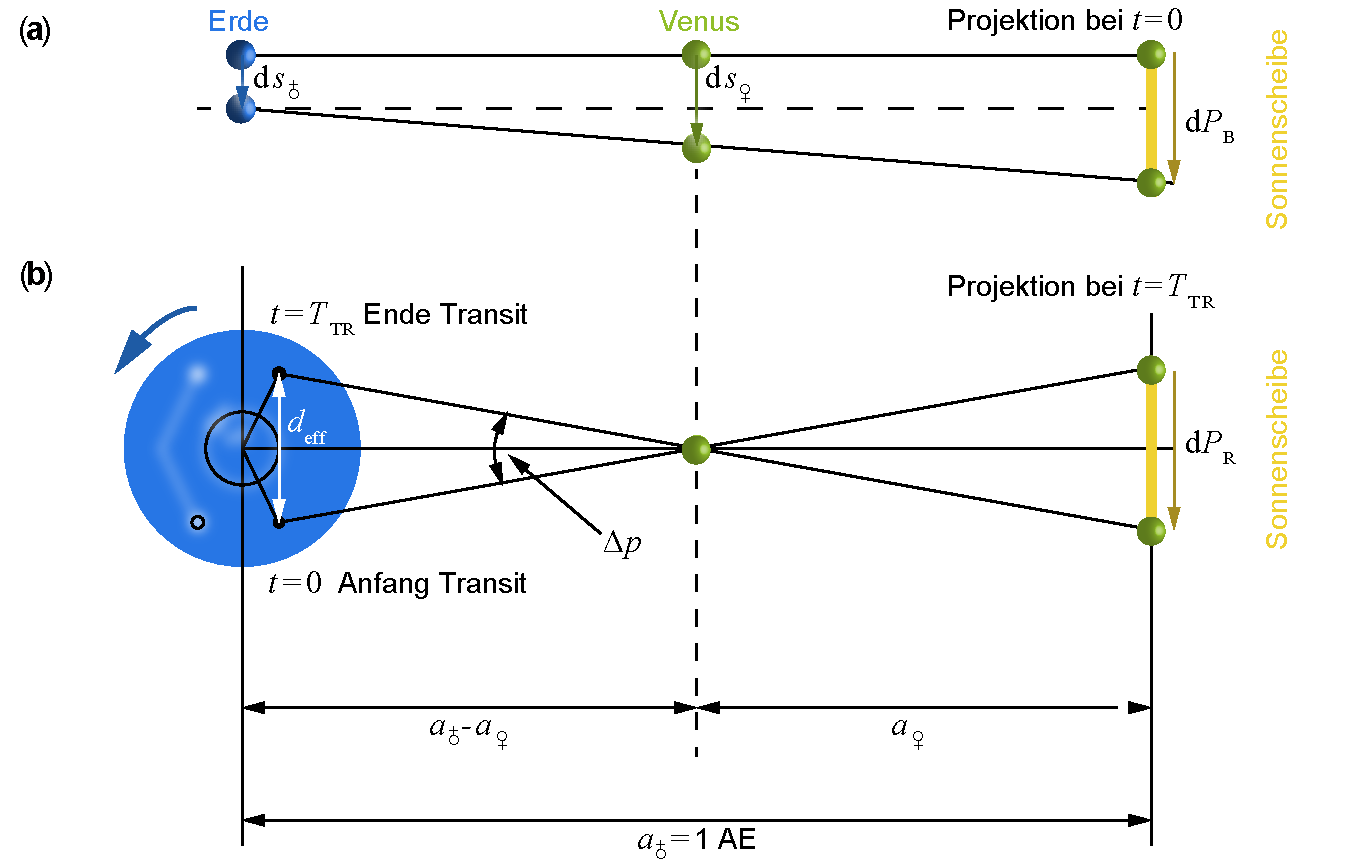
\includegraphics[width=\textwidth]{Venustransitd.pdf}
\captionof{figure}[Schematische Darstellung der Kontaktzeitmethode.]{Schematische Darstellung der Kontaktzeitmethode.
Betrachtung der Venus-Projektionen \fa ohne \fb mit Erdrotation.}\label{abb:hm_VenusTransitd}
\end{center}

Jetzt kommt noch die Erdrotation ins Spiel, die uns wiederum eine Parallaxe liefert.
Anstelle der r�umlichen Differenz zweier Beobachter zum gleichen Zeitpunkt m�ssen wir jetzt die r�umliche Differenz eines ortsfesten Beobachters zu zwei Zeiten betrachten.
Aus \figref{hm_VenusTransitd}b erkennen wir, dass die Erdrotation eine zus�tzliche Winkelgeschwindigkeit $\Omega_\text{B}$ f�r die Projektion bewirkt, die sich �ber 
\begin{equation*}
\frac{d_\text{eff}}{a_\text{\earth} - a_\text{\venus}} = \frac{\D P_\text{R}}{a_\text{\venus}}
\end{equation*}	
berechnet zu 
\begin{equation*}
\Omega_\text{R} = \frac{1}{a_\text{\earth}} \frac{\D P_\text{R}}{\D t} = \frac{d_\text{eff}}{T_\text{TR} a_\text{\earth} \lk \gamma -1 \rk}  \,.
\end{equation*}	
Die reale von einem Beobachter auf der Erdoberfl�che gemessene Transitzeit ist daher gegeben durch
\begin{align*}
T_\text{TR,B} &= \frac{b_\text{w\astrosun} \, l_\text{S\astrosun}}{\Omega_\text{B} + \Omega_\text{R}}
= \frac{b_\text{w\astrosun} \, l_\text{S\astrosun}}{\Omega_\text{B} + \lek d_\text{eff} / \lk T_\text{TR,B} \:  a_\text{\earth} (\gamma -1) \rk \rek} \; .
\end{align*}
Auch hier haben wir wieder eine Bestimmungsgleichung f�r die Astronomische Einheit in einer Abh�ngigkeit zu bekannten terrestrischen Distanzen ($d_\text{eff}$) und einer Zeitmessung erhalten:
\begin{equation}
1 \text{AE}\!=\!a_\text{\earth} \!=\!\frac{d_\text{eff}}{(\gamma - 1 )\lk b_\text{w\astrosun} \, l_\text{S\astrosun} - \Omega_\text{B} \, T_\text{TR,B} \rk}  \,.\label{eq:hm_Venus_AE_KontaktMessung}
\end{equation}
Die Gr��en $b_\text{w\astrosun}$, $\Omega_S$ und $\gamma$ sind bekannt.
$l_\text{S\astrosun}$ und $T_\text{TR,B}$ werden gemessen.
Damit man eine ausreichende Genauigkeit bei der Bestimmung der Astronomische Einheit bekommt, muss man die Sehnenl�nge $l_\text{S\astrosun}$ und vor allem $T_\text{TR,B}$ sehr genau bestimmen, da der Nenner in \eqref{eq:hm_Venus_AE_KontaktMessung} gegen Null geht.
Das ist die eigentliche Herausforderung dieser Methode.
In \probref{hm_venus_2004_2012} berechnen wir f�r Messwerte von 2004 nach dieser einfachen Methode den Wert der AE.
Zudem verfeinern wir die Methode, indem wir die Annahmen konzentrischer und koplanarer Kreisbahnen fallen lassen. \\

\end{enumerate}
\label{bsp:venustransit}
\end{example}
%BEISPIEL %%%%%%%%%%%%%%%%%%%%%%%%%%%%%%%%%%%%%%%%%%%%%%%%%%%%%%%%%%%%%%%%%%%%%%%%%%%%%%%%%%

Analog zu Venustransits gibt es auch Merkurtransits.
Diese sind auf Grund der k�rzeren Umlaufperiode des Merkurs naturgem�� h�ufiger.
Sie erlauben ebenfalls die Bestimmung der Astronomischen Einheit, allerdings mit geringerer Pr�zision.
Die letzten Merkurtransits wurden in Europa im Mai 2016 und im November 2019 beobachtet, und den n�chsten wird es schon wieder 2032 geben.
Das wirft die Frage auf, ob es auch gemeinsame Transits von Merkur und Venus vor der Sonne geben kann.
Tats�chlich gibt es solche und der n�chste wird \anf{schon} am 26.\,07.\,69163 beobachtbar sein \cite{Meeus2004}.
F�r solche gro�en Zeitabst�nde reicht die Genauigkeit unserer Rechnung allerdings nicht aus.
Die f�r den 22.\,11.\,2065 vorhergesagte Bedeckung des Planeten Jupiter durch die Venus ist hingegen mit unserer einfachen Keplerrechnung (\probref{hm_jupiterbedeckung_venus}, \mscr{} \mlhmref{InnerePlaneten.m}) zumindest prinzipiell vorhersagbar.
F�r die Bestimmung der genauen Beobachtungszeiten und -koordinaten reicht das aber nicht mehr aus.
Dazu braucht man genauere Ephemeriden.
Wir werden uns deswegen jetzt mit den grundlegenden Prinzipien der St�rungsrechnung besch�ftigen, mit welcher man genauere Planetenbahnen auch �ber l�ngere Zeiten berechnen kann.
Zun�chst aber wollen wir uns noch mit dem Mehrk�rperproblem etwas genauer besch�ftigen, das wir bereits in der Physik der Bewegung (Band I, Kapitel 1) vorgestellt und f�r Spezialf�lle (eingeschr�nktes Dreik�rperproblem) behandelt hatten.

\subsection{Das Mehrk�rperproblem}\index{Mehrk�rperproblem} \label{kap:mehrkoerperproblem}

So einfach und elegant die Bahnberechnung auf Basis des Zweik�rperproblems\index{Zweik�rperproblem} auch ist, die Nichtber�cksichtigung von St�rungen der einfachen Keplerbahn durch andere Himmelsk�rper stellt eine echte Begrenzung f�r die Berechnung vieler realer Situationen in der Astronomie dar.
Der logische Schritt w�re daher, die Bewegungsgleichung \eqref{eq:hm_beschl_zk} auf $N$ K�rper (\figref{hm_Nkp} als Beispiel f�r $N\!=\!3$) zu erweitern.
Wir starten daher mit dem allgemeinen Ansatz
\begin{equation}
\vec{F}_i = m_i\,\ddot{\vec{r}}_i= -\sum_{j=1,j\neq i}^N \frac{G \, m_i m_j}{\left|\vec{r}_j - \vec{r}_i\right|^3}\cdot (\vec{r}_j - \vec{r}_i) \ \  ~~\text{f�r}~i=1,\ldots,N.\\
\label{eq:hm_beschl_N_koerper}\
\end{equation}

\begin{figure}
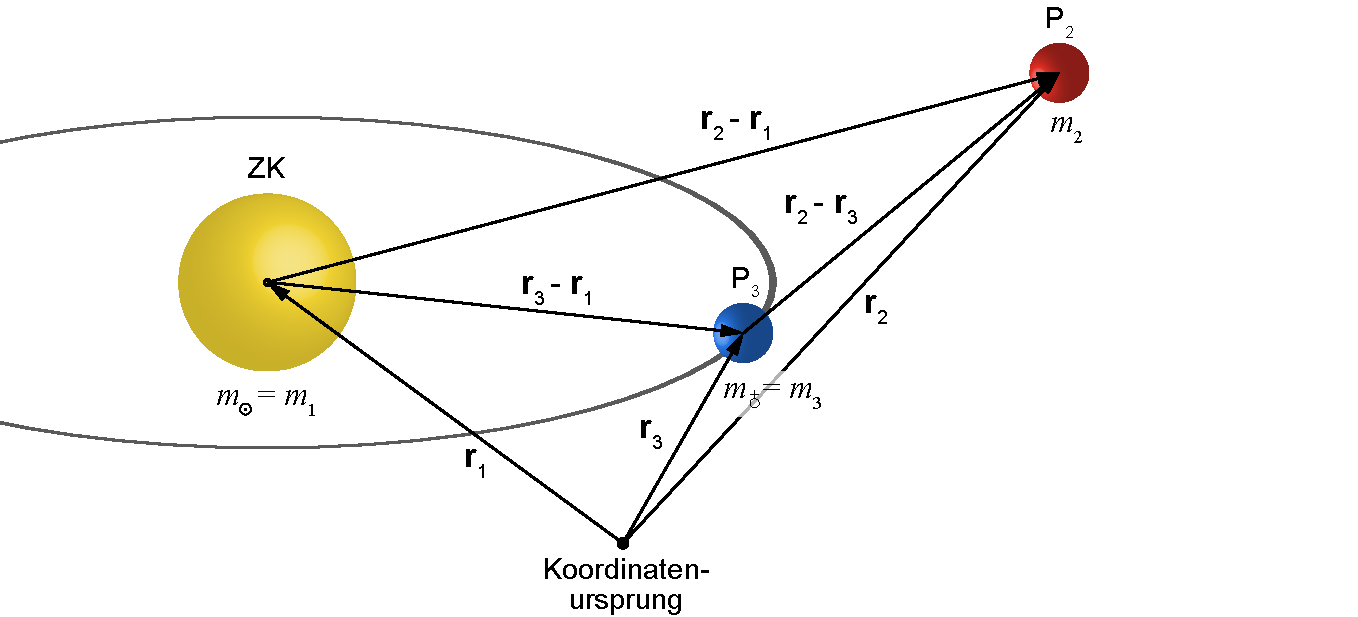
\includegraphics[width=\textwidth]{NKP.pdf}%
\caption[Geometrie eines Mehrk�rperproblems.]{Geometrie eines Mehrk�rperproblems am Beispiel der St�rung der Erdbahn durch einen weiteren �u�eren Planeten. ZK = Zentralk�rper ist in den folgenden Betrachtungen die Sonne, $\text{P}_3$ die Erde und $\text{P}_2$ ein �u�erer Planet oder der Erdmond.}
\label{abb:hm_Nkp}%
\end{figure}

Wie schon in Band I gezeigt, ist schon das Dreik�rperproblem ($N=3$) bis auf Spezialf�lle nicht mehr geschlossen analytisch l�sbar.
Es k�nnen daher auch keine geschlossenen Bewegungsgleichungen wie die Kepler-Gleichung\index{Kepler-Gleichung} f�r ein vermeintlich einfaches System, wie z.\,B. Sonne, Mond und Erde mehr angegeben werden. Es gibt aber f�r bestimmte Spezialf�lle L�sungen (siehe Band I), die physikalisch interessante und auch f�r die Praxis (\zb die Raumfahrt) relevante Schlussfolgerungen erlauben. 

\subsubsection{Ans�tze zur Behandlung des Mehrk�rperproblems}\label{kap:stoerungsrechnung}

F�r das \textit{allgemeine} Mehrk�rperproblem ohne Einschr�nkungen gibt es nun drei grunds�tzliche Ans�tze, mit denen man das (nichtlineare) System aus $3N$ Differentialgleichungen zweiter Ordnung basierend auf \eqref{eq:hm_beschl_N_koerper} behandeln kann: 
\begin{itemize}
	\item eine \emph{allgemeine St�rungstheorie}, die auf \emph{analytische Reihenentwicklungen} f�hrt,
	\item eine \emph{numerische Integration} und 
	\item \emph{spezielle St�rungstheorien}, die die numerische Integration vorbereiten.
\end{itemize}

Jede dieser Methoden hat ihre spezifischen Einsatzbereiche.
Die allgemeine St�rungstheorie mit ihren analytischen Reihenentwicklungen wird meist in der Planetentheorie benutzt, w�hrend die numerische Integration \zb bei der Berechnung von Kometen- und Asteroidenbahnen und auch in der Raumfahrt eingesetzt wird.
Wir stellen im Folgenden nur die Grundz�ge der beiden ersten Methoden dar. 
%Mit einigen speziellen St�rungsrechnungen werden wir uns im Kap. Astrodynamik (Kap. \ref{chap:adyn}) besch�ftigen. 
F�r eine ausf�hrliche Behandlung empfehlen wir als weiterf�hrende Literatur \ua die Darstellungen in \cite{Fitzpatrick2022, Walter2018, Guthmann2000, Brouwer1961, Murray2008}.\footnote{Eine sehr sch�ne und kompakte Darstellung der Effekte einer st�renden Kraft auf die Keplerbahn findet man in \cite{Burns1976}. In dieser Darstellung werden die Effekte �ber die Wirkung der St�rungskraft auf den Drehimpuls des ZKP beschrieben. Wir empfehlen diese Darstellung als gute physikalische Einf�hrung in die Methode der St�rungsrechnungen.} 

\subsubsection{Grundidee der allgemeinen St�rungsrechnung (analytische Reihenentwicklungen)}\index{Reihenentwicklung}\index{St�rungsrechnung}  \label{kap:Reihenentwicklung}

Wir starten von den Annahmen, dass 
\begin{itemize}
	\item die St�rungen relativ klein sind,
	\item die Massen der beteiligten Himmelsk�rper relativ weit voneinander entfernt sind und
	\item die Bahnen der Himmelsk�rper kleine Exzentrizit�ten haben und hinreichend stabil sind.
\end{itemize}
Letztere Annahme werden wir in den sp�teren Kapiteln \ref{kap:Periheldrehung} und \ref{kap:hm_langezeiten} noch etwas genauer betrachten.
Unter diesen Annahmen kann man die Bahnen als �berlagerung ungest�rter, sogenannter mittlerer Kepler-Ellipsen und kleiner periodischer St�rungen, sogenannter St�rterme, darstellen.
Wir hatten ja schon im vorhergehenden Kapitel gesehen, dass sich die ekliptikalen Koordinaten $l(t)$, $b(t)$, $r(t)$ als Funktion der Zeit (bzw. der mittleren Anomalie) in einer Reihenentwicklung angeben lassen (siehe Gleichungen \eqref{eq:hm_reduktions_formel4}--\eqref{eq:hm_reduktions_formel6}).
Die St�rungen durch den anderen Planeten ergeben nun zus�tzliche Terme in dieser Reihenentwicklung, welche als Argument die mittlere Anomalie des \bzw der \anf{st�renden} Himmelsk�rper und die des gest�rten Planeten, dessen Bahn wir berechnen wollen, enthalten.\footnote{Die mittleren Anomalien aller Planeten sind in Tabelle \ref{tab:hm_bahnparameter} angegeben.
Die Betrachtungen, die wir im Folgenden f�r den Fall $N\!=\!3$ anstellen, lassen sich ohne weiteres auf allgemeine F�lle $N>3$ �bertragen.}

\subparagraph{\textbf{Die St�rungsfunktion am Beispiel des Dreik�rperproblems }}\index{Dreik�rperproblem}\index{St�rungsfunktion} \label{kap:stoerungsfunktion} 
 
Ein relativ einfacher und instruktiver Fall ist das koplanare Dreik�rperproblem (siehe Kapitel 1.2.3.5 im Band I). Selbst dieses Problem erfordert schon eine anspruchsvolle mathematische Behandlung und l�sst erahnen, welche mathematische technische Komplexit�t hinter der St�rungsrechnung liegt. 
Wir verweisen hier auf die Spezialliteratur und empfehlen insbesondere \cite{Fitzpatrick2022} und \cite{Murray2008}.\\
%Wir skizzieren hier nur die generelle Vorgehensweise und verweisen ansonsten auf die Spezialliteratur cite{Fitzpatrick2022, Murray2008}.\\

\subparagraph{\textbf{Standard-St�rungsrechnungen und Tabellen}} \label{kap:stoerungstabellen}

Die berechneten St�rungsterme, wie im vorhergehenden Teil skizziert,  werden \ia in umfangreichen Tabellen angegeben (\ua \cite{Montenbruck1999, Murray2008}).
Es ist eine der gro�en Leistungen vieler Generationen von Astronomen, Mathematikern und Physikern, die mit diesen analytischen Reihenentwicklungen -- die oft hunderte von Termen umfassen -- hochgenaue Berechnungen f�r die Planeten ermittelt und damit auch ganz wesentlich zum Erkenntnisfortschritt in der Physik und Astrophysik beigetragen haben (siehe \kapitel{Periheldrehung}).\footnote{Man mache sich klar, dass diese Rechnungen bis in die Mitte des 20.\ Jahrhunderts ohne elektronische Computer gemacht wurden. Man sprach auch davon, dass Astronomie im 18.\ und 19.\ Jahrhundert \iw Rechnen war, wof�r sehr oft Frauen als sogenannte \anf{Computer} eingesetzt wurden. Viele dieser Frauen leisteten sp�ter wichtige eigenst�ndige Beitr�ge in der Astronomie und Astrophysik.}
Dar�ber hinaus gab es aber auch ganz praktische und �konomisch hochrelevante Beweggr�nde f�r diese enorme Arbeit.
So waren die genauen Berechnungen der (scheinbaren) Sonnenbahn und der Mondbahn f�r die maritime Navigation erforderlich.
%Deswegen wurde gerade in diese theoretischen Berechnungen entsprechend viel Aufwand gesteckt.
Die von Simon Newcomb\footnote{Simon Newcomb (1835--1909) war ein kanadischer Astronom und Mathematiker, der am Observatorium der US-Marine in Washington, D.\,C.\ zur Theorie der scheinbaren Bewegung der Sonne und zur Bestimmung der Planetenpositionen als Navigationshilfe arbeitete.}\indexp{Newcomb, Simon} entwickelte Theorie zur scheinbaren Sonnenbewegung ist heute noch ein Standard, weswegen wir die wesentlichen Terme in \mlhmiref{SonneExakt.m} (\zb zur Berechnung von Sonnenfinsternissen) mit angegeben haben.
Die Berechnung der Mondbahn ist im Vergleich zur St�rungsrechnung f�r die Planetenbahnen noch etwas komplexer, da die Gravitationskr�fte von Sonne und Erde auf den Mond etwa gleich gro� sind.
Dennoch kann man das Prinzip der Reihenentwicklung auch hier anwenden.
Danach ist die mittlere Mondbahn in grober N�herung eine Ellipse mit Exzentrizit�t $e\!=\!0.0549$ und Neigung $i\!=\!5.145\degree$ gegen die Ekliptik.
Viele der periodischen Mondbahnabweichungen von dieser Ellipsenbahn waren schon im Altertum bzw. Mittelalter bekannt.
In \mlhmiref{MondExakt.m} haben wir wiederum die wichtigsten Terme der Mondbahn nach der von Ernest~W.~Brown\indexp{Brown, Ernest William}\footnote{Ernest William Brown (1866--1938) war ein US-amerikanischer Mathematiker und Astronom.
Seine Theorie �ber die Bewegung des Mondes galt bis \ca 1985 als bestes Modell und war die mathematische Grundlage der NASA-Mondlandung.} Anfang des 20.\ Jahrhunderts entwickelten Mondtheorie angegeben. 
In den \textbf{�bungen} \ref{prob:hm_jupiterbedeckung_venus} und \ref{prob:hm_Zusatz_ErdeTransit_from_Mars} kann man anhand der Berechnung der Jupiterbedeckung durch die Venus am 22.\,November\,2065 \bzw des Erdtransits am 10.\,November\,2084 vom Mars aus gesehen sehr sch�n die Unterschiede in der Genauigkeit zwischen der einfachen Keplerl�sung und der Berechnung �ber die Reihenentwicklung nach der St�rungstheorie erkennen. 

In den \mscren \mlhmref{Sonnenfinsternis01.m} und \mlhmref{Sonnenfinsternis02.m} haben wir neben den Koordinatenberechnungen f�r Sonne und Mond nach der Newcombschen \bzw Brownschen Theorie auch f�r die einzelnen Planeten die \mscre \mlhmiref{SonneExakt.m}, \mlhmiref{MondExakt.m}, \mlhmiref{VenusExakt.m} \usw hinterlegt: Die ersten Terme der Reihenentwicklung finden sich in den Dateien \mlhmdref{VenusPos.csv} \usw \cite{Montenbruck1999, Meeus1998}. Damit lassen sich Berechnungen mit maximalen Fehlerabweichungen von wenigen Bogensekunden �ber viele Jahre realisieren.

\subsubsection{Berechnung von Himmelsk�rperbahnen durch numerische Integration}\index{Numerische Integration}\label{kap:hm_numerische_proced}

Im Gegensatz zu den Reihenentwicklungen wird bei den numerischen Verfahren versucht, die Bahnberechnung der einzelnen Massen durch die direkte numerische Integration aller Bewegungsgleichungen \eqref{eq:hm_beschl_N_koerper} zu realisieren.
Zur Integration dieser Bewegungsgleichungen gibt es verschiedene Verfahren \cite{Press2007}, von denen einige in \matlab{} hinterlegt sind.
Das Grundprinzip dieser Verfahren f�r ein Differentialgleichungssystem 2.~Ordnung ist ausf�hrlich im Kapitel 1.3.1 im Band I und in den \onlineZ{} erl�utert. 
Bei der Anwendung im astronomischen Bereich ist auf ausreichende Genauigkeit und Stabilit�t der L�sung zu achten, insbesondere bei Anwendung der Verfahren mit variabler Schrittweite, bei denen zum einen die zeitlichen Ver�nderungen mit ausreichender Genauigkeit berechnet werden muss und zum anderen aber die Rechenzeit optimiert werden soll.\\
Heute werden in den Gro�rechenzentren der astronomischen Institute leistungsstarke Rechner und Programme eingesetzt, um die Ephemeriden\index{Ephemeride|textbf} von Himmelsk�rpern zu berechnen.
Das Jet Propulsion Laboratory \cite{JPL2020} ist ein Paradebeispiel daf�r.
Die analytischen Reihenentwicklungen wurden mithilfe der Computertechnik ebenfalls weiter entwickelt und haben im Vergleich zur Mitte des 20.~Jahrhunderts eine viel gr��ere Genauigkeit.
Beispiele sind hier die semi-analytische Mondbahnberechnung der ELP (\emph{Ephemeride Lunaire Parisienne}) \cite{ELP2020} und die VSOP (\emph{Variations S�culaires des Orbites Plan�taires}), eine wiederum semi-analytische Theorie f�r die Planetenbahnen, in der komplexe analytische Reihenentwicklungen mit effizienten numerischen Approximationsmethoden verbunden werden \cite{VSOP2020}. 

Wir wollen anmerken, dass f�r fast alle �bungen und Beispiele in diesem Buch die in \matlab{} implementierten leistungsstarken numerischen Verfahren zur Integration von Differentialgleichungen des beschriebenen Typs vollkommen ausreichend sind. 
Wir berechnen im Folgenden exemplarisch die Bahn des Kometen Shoemaker-Levy 9\index{Komet!Shoemaker-Levy}\indexp{Shoemaker, Eugene Merle}\footnote{Eugene Merle Shoemaker (1928--1997) war ein US-amerikanischer Geologe, Impaktforscher und Astronom. Bekannt wurde er als Mitentdecker des Kometen Shoemaker-Levy 9 (mit seiner Frau Carolyn Shoemaker und David H.~Levy). Er konnte in seinen geologischen Forschungen nachweisen, dass der Barringer-Meteorkrater in den USA und tats�chlich auch das N�rdlinger Ries durch einen Meteoriteneinschlag entstanden sind. 1969 war er auch Chefwissenschaftler der Apollo-11-Mission.} (\kapitel{kometen}), der sich in der N�he eines Planeten befindet und dessen Bahn daher massiv durch diesen gest�rt wird. Aus der Beobachtung seiner Bahn wurde bald klar, dass dieser vom Jupiter eingefangen werden w�rde. Im Gravitationsfeld des Jupiters zerbrach der Komet dann durch die Wirkung von Gezeitenkr�ften (siehe \kap{hm_gezeiten}) in rund $\SI{100000}{\km}$ Entfernung in 21 Fragmente bis zu $\SI{1}{\km}$ Gr��e. Wir wollen hier das Fragment D/1993 F2  betrachten. (Das \anf{D} in seiner Bezeichnung steht f�r \anf{disappeared}.)

%BEISPIEL 4 %%%%%%%%%%%%%%%%%%%%%%%%%%%%%%%%%%%%%%%%%%%%%%%%%%%%%%%%%%%%%%%%%%%%%%%%%%%%%%%%%%
\begin{example}{Shoemaker-Levy 9 (D/1993 F2)} \label{bsp:hm_shoemaker_levy}
\textit{Wir wollen die durch den Jupiter gest�rte Bahn des Kometen Shoemaker-Levy 9\index{Komet!Shoemaker-Levy} (D/1993 F2) in heliozentrischen Koordinaten berechnen.}
Aus den berichteten Beobachtungsdaten f�r Shoemaker-Levy 9 finden wir die Position und Geschwindigkeit des Kometen
in ekliptikalen Koordinaten zu den Zeiten  $t_1\equiv 01.01.1993$ und $t_2\equiv 02.01.1993$ jeweils um 00:00 ET:
\begin{align*}
	l_1&= 181.1041\degree~,\; b_1 = -0.5639\degree~,\; r_1 = 5.478189665071 \:\text{AE} ~,\\
	l_2&= 181.1747\degree~,\; b_2 = -0.5688\degree~,\; r_2 = 5.478141861326 \:\text{AE} ~.
	\end{align*}
Daraus k�nnen wir die kartesischen heliozentrischen Koordinaten $(x_1,y_1,z_1), (x_2,y_2,z_2)$ gewinnen und daraus wiederum durch Differenzenbildung n�herungsweise die Anfangsgeschwindigkeit $(\dot x_1,\dot y_1,\dot z_1)$ und damit den Anfangsvektor f�r unsere numerischen Berechnungen zu
\begin{equation*}
\lk \dot x_1,\dot y_1,\dot z_1 \rk = \lk x_2 - x_1, y_2 - y_1, z_2 - z_1 \rk \:/ \:\text{1d} \,,
\end{equation*}	
\begin{align*}
\vec{\psi}(t_0) &= \lk \begin{array}{c} -5.476907295330\:\text{AE}\\ -0.105554056709 \:\text{AE}\\ -0.053914988291\:\text{AE}\\ +0.000186643064 \: \text{AE/d}\\ -0.006747501846\: \text{AE/d}\\ -0.000468003540\: \text{AE/d} \end{array}\rk\,.
\end{align*}
Vergleicht man zu diesem Zeitpunkt die Gravitation der Sonne \bzw des Jupiters auf den Kometen, so ergibt sich bereits zu $t_0$ ein Verh�ltnis von
\begin{equation*}
\frac{F_{\jupiter}}{F_{\astrosun}} = \frac{m_{\jupiter}}{m_{\astrosun}} \cdot \frac{\vec{r}_\text{K}^2}{\left| {\vec{r}_\text{K}-\vec{r}_{\jupiter} }\right|^2} = 7.978 \,.
\end{equation*}	

\begin{center}
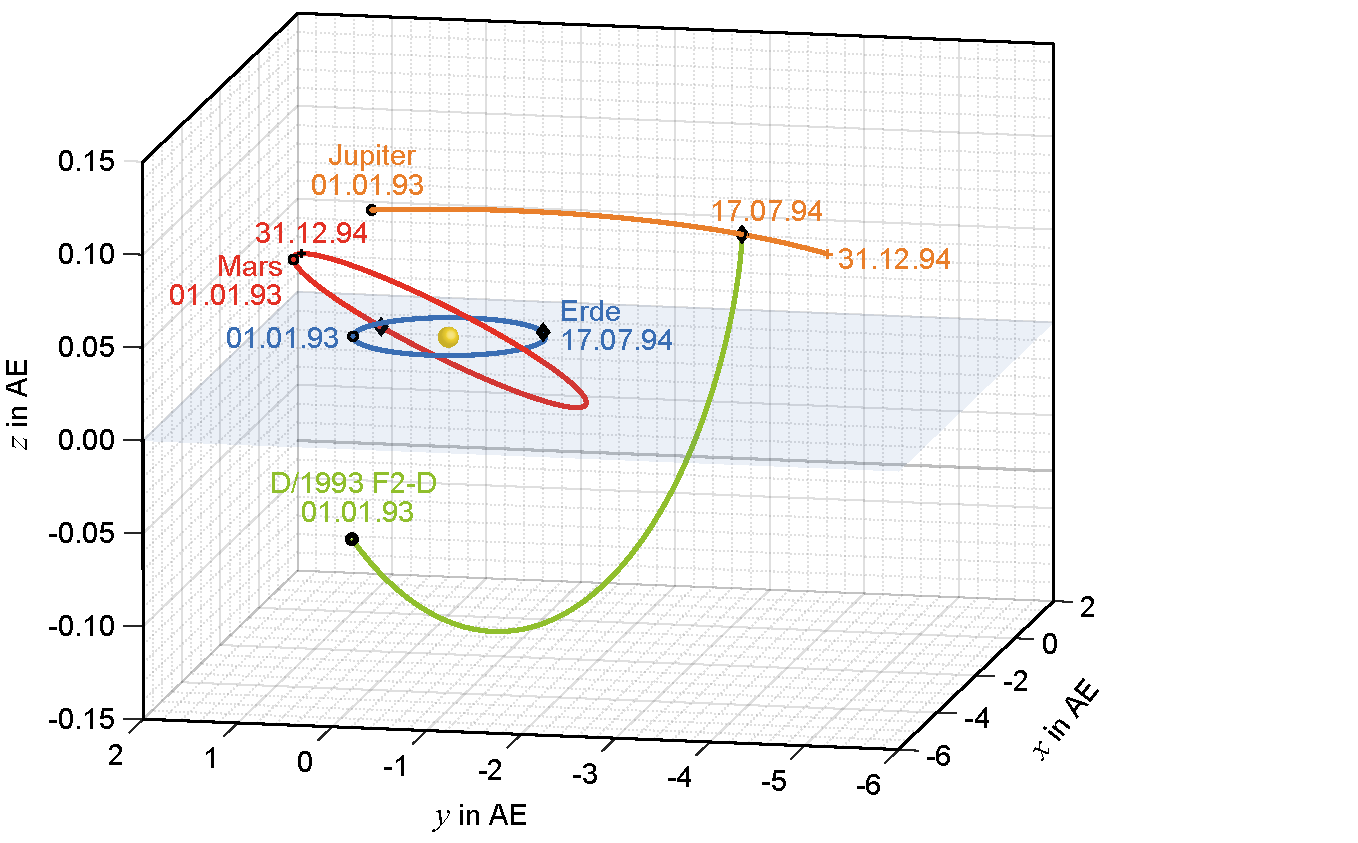
\includegraphics[width=\columnwidth]{SL9b_Variante.pdf} 
\captionof{figure}[Bahn des Kometen Shoemaker-Levy 9 in den Jahren 1993/94.]{Bahn des Kometen Shoemaker-Levy 9 in den Jahren 1993/94 bis zum Aufschlag auf den Jupiter.}\label{abb:hm_SL9Bahn}
\end{center}

Die Rechnung zeigt, dass der Komet sich bereits zu diesem Zeitpunkt im \anf{Einfangbereich} des Jupiters befand und dass eine dramatische Zunahme der Kr�fte des Jupiters $F_{\jupiter}$ zu erwarten war. 
Wir k�nnten nun mit den Anfangswerten an die L�sung des Dreik�rperproblems mit dem bekannten und in den \onlineZ{} beschriebenen \textit{Runge-Kutta-Verfahren}\index{Runge-Kutta-Verfahren} gehen, k�nnen das Problem aber etwas vereinfachen, da wir die Bahn des Jupiters als weiterhin ungest�rt annehmen k�nnen.
Wir benutzen deshalb in \mlhmref{SL9numerisch.m} auch die in \matlab{} hinterlegten Routinen (\zb \textcolor{mygreen}{\texttt{ode45}}) zur L�sung des Differentialgleichungssystems f�r $\vec{\psi}(t)$.
Das Ergebnis der Berechnung ist in \figref{hm_SL9Bahn} zu sehen.
Mit guter Genauigkeit berechnet das Programm den Zusammenprall von SL9 (D/1993 F2) f�r den 17.\,07.\,1994 um 20:35 UT.
Der so berechnete Zeitpunkt weicht nur wenig vom tats�chlich beobachteten Zeitpunkt 18.\,07.\,1994, 00:35 UT ab. 
Aus den Rechnungen wird allerdings auch deutlich, wie extrem kritisch die Ergebnisse von den Anfangsparametern (Ort und Geschwindigkeit des Kometen) und der Masse des Jupiters abh�ngen.
In \figref{hm_SL9Bahnberechnung} haben wir diese Parameter etwas variiert.
Es zeigt sich, dass im Fall einer h�heren Jupitermasse der Komet erwartungsgem�� fr�her auf den Jupiter aufschlagen w�rde.
In den F�llen der um 20\% erh�hten oder ver�nderten Anfangsgeschwindigkeiten des Kometen w�rde dieser den Jupiter aber \anf{verfehlen}.
Dies zeigt noch einmal deutlich, wie wichtig hochgenaue Beobachtungsdaten f�r Berechnungen in der Himmelsmechanik sind. \\

\begin{center}
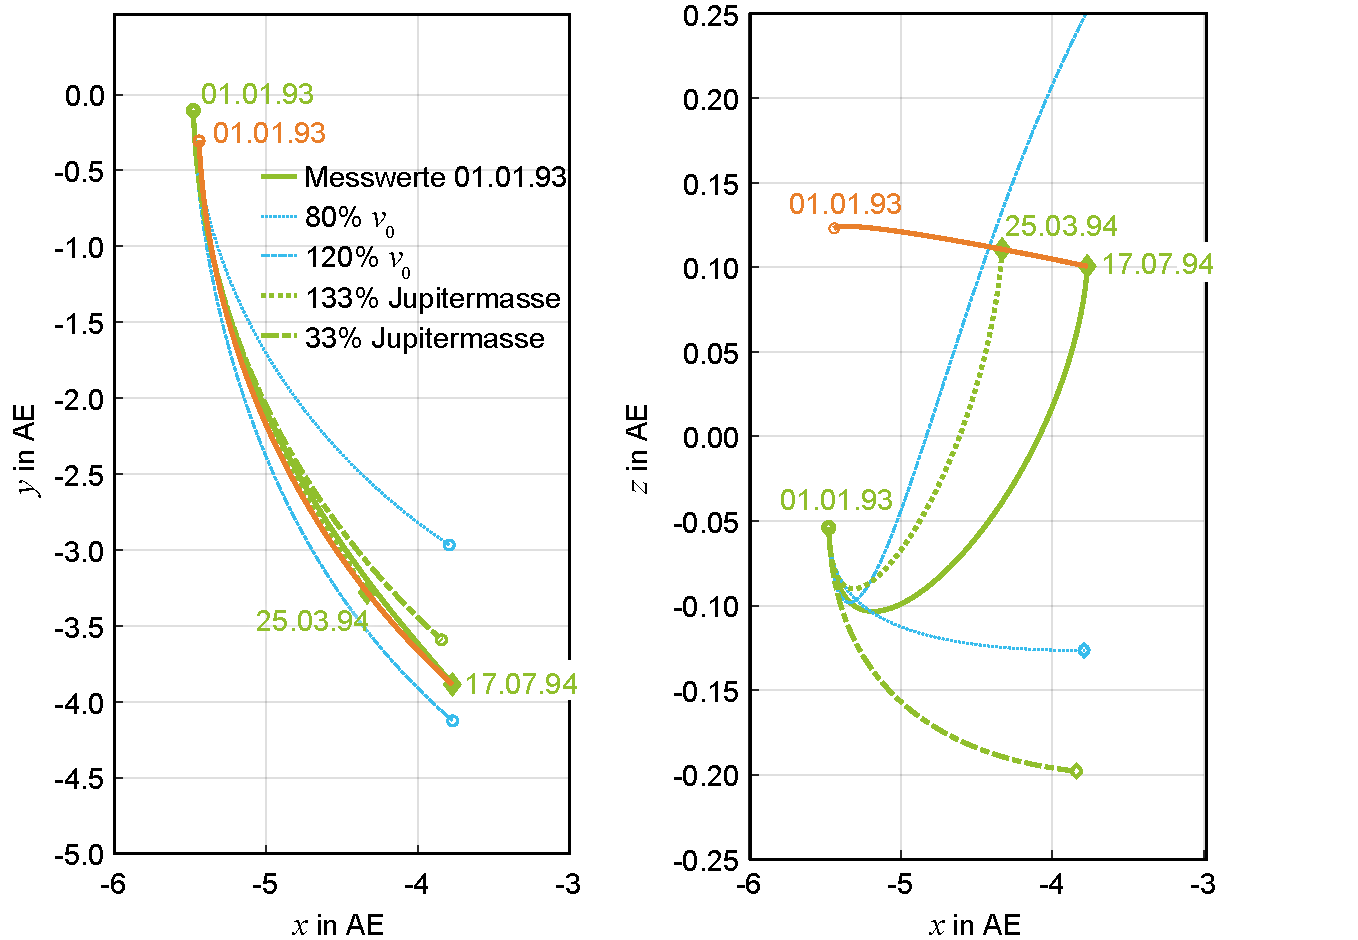
\includegraphics[width=\textwidth]{SL9a.pdf}
\captionof{figure}[Bahnberechnung des Kometen Shoemaker-Levy 9 in den Jahren 1993/94.]{Bahnberechnung des Kometen Shoemaker-Levy 9 in den Jahren 1993/94 mit verschiedenen Annahmen f�r Jupitermasse und Anfangsgeschwindigkeiten.}\label{abb:hm_SL9Bahnberechnung}
\end{center}

Zum Schluss berechnen wir noch, mit welcher Geschwindigkeit der Komet auf den Jupiter prallt.
Unsere numerischen Rechnungen ergeben f�r den letzten Rechenschritt vor dem Zusammenprall 
\begin{align*}
\vec{v}_\text{SL9} &= \lk \begin{array}{c} +0.013395176\\ +0.006460533 \\ -0.029725683 \end{array}\rk \:\text{AE/d} \;\: \text{bzw.}\ \;\vec{v}_{\jupiter} = \lk \begin{array}{c} +0.005323551\\ -0.004907594 \\ -0.000098762 \end{array}\rk \:\text{AE/d} 
\end{align*}
eine Aufprallgeschwindigkeit von
\begin{equation*}
  v_\text{impact} = \sqrt{\left|{\vec{v}_\text{SL9}-\vec{v}_{\jupiter}}\right|^2} \approx \SI{57.1}{\kilo\metre\per\second}~.
\end{equation*}
Diese Geschwindigkeit liegt nahe an der 2.~kosmischen Geschwindigkeit\index{Geschwindigkeit!2.~kosmische} des Jupiters von 
\begin{equation*}
  v_\text{escape} = \sqrt{\frac{2 G\, m_{\jupiter}}{R_{\jupiter}}}\approx \SI{59.5}{\kilo\metre\per\second}~,
\end{equation*}
was verst�ndlich ist, da der Komet den Jupiter auf dessen Bahn unter einem Winkel von nahezu $90\degree$ trifft.
Hierin ist $R_{\jupiter}$ der Radius des Jupiters.
Aus \cite{Crawford1996} k�nnen wir die Gesamtgr��e des Kometen vor dem Zerbrechen mit $\SI{1.4}{\kilo\metre}$ entnehmen.
Mit einer mittleren Dichte von $\SI{0.5}{\gram\per\centi\metre^3}$ ergibt sich daraus eine kinetische Aufprallenergie von $\SI{1.17e21}{\joule}$.
Das entspricht einer unglaublichen \anf{Explosionskraft} von \ca \SI{280}{\giga\tonne} TNT, was gleichbedeutend mit der Sprengkraft von etwa 18 Millionen Hiroshima-Bomben ist.\\

\end{example}
%%BEISPIEL %%%%%%%%%%%%%%%%%%%%%%%%%%%%%%%%%%%%%%%%%%%%%%%%%%%%%%%%%%%%%%%%%%%%%%%%%%%%%%%%%%

Obwohl offensichtlich ist, dass die in Beispiel \ref{bsp:hm_shoemaker_levy} berechnete Bahn des Kometen erheblich von einer reinen Keplerbahn abweicht, werden wir im \kap{kometen} sehen, dass man f�r n�herungsweise Berechnungen von weniger gest�rten Kometenbahnen durchaus die Keplerl�sung mit effektiven Bahnparametern benutzen kann.
\subsection{Periheldrehung des Merkurs}\index{Periheldrehung} \label{kap:Periheldrehung}
Wie wir gesehen haben, gibt es gravitative Einfl�sse der anderen Planeten auf ein ideales ZKP (reines Sonne-Planet-System), die zu St�rungen der reinen Keplerl�sungen und -ellipsen f�hren.
Wir wollen eine dieser St�rungen -- die auch wissenschaftshistorisch sehr interessant ist -- in diesem Kapitel etwas genauer betrachten.
Wir m�chten uns aber zun�chst der Frage zuwenden, unter welchen Bedingungen wir bei vorhandenen St�rungen �berhaupt von stabilen und geschlossenen Bahnen sprechen k�nnen.
Unter \anf{stabil} verstehen wir, dass der Radius $r$ der Bahn �ber die Zeit in einem endlichen Bereich bleibt.
Unter \anf{geschlossen} verstehen wir, dass es einen ausgezeichneten Punkt der Bahn gibt (\zb das Perihel), der sich nach einem vollen Umlauf $T_\text{P}$ wieder an derselben Position befindet, also $\lek r(t_0+T_\text{P}), \upsilon(t_0+T_\text{P})\rek\!=\!\lek r(t_0), \upsilon(t_0) \rek$.

\subsubsection{Bedingungen f�r stabile und geschlossene Bahnen}\index{Bahn!geschlossene}\index{Bahn!stabile} \label{kap:Stabile_Bahnen}
Wir wollen nun ein allgemeines Gravitationspotential $U_\text{\,ZK}(r)$ annehmen, welches aber immer noch ein \gls{zkf}\index{Zentralkraftfeld} (ZK) repr�sentiert.
Die Bewegung findet wegen der weiterhin geltenden Drehimpulserhaltung in einer Ebene statt.
Die Bewegung eines Planeten mit Masse $m$ in diesem ZK kann durch folgendes Potential eines Gravizentrums\footnote{Hierbei haben wir wie bisher auch das \pot{} auf die Masse $m$ \anf{normiert}. Wir werden sp�ter im Kapitel, wenn es um die Berechnung von Merkur-Messwerten geht, die entsprechenden Gr��en mit der Masse des Merkurs $m_{\mercury}$ multiplizieren.} beschrieben werden:
\begin{align}
%U_\text{Z}(r) &= -\frac{\mu_\text{G}}{r} + \frac{\kappa_2}{r^2} + \frac{\kappa_3}{r^3} +\ldots = -\frac{\mu_\text{G}}{r} + \sum \limits_{i}{} \Delta U_i(r) \,, \label{eq:hm_bwg_allg_ZK}
U_\text{\,ZK}(r) &= -\frac{\mu_\text{G}}{r} + \sum \limits_{i}{} \Delta U_i(r) \,. \label{eq:hm_bwg_allg_ZK}
\end{align}
Daraus ergibt sich folgende allgemeine Bewegungsgleichung:
\begin{equation}
%\vec{b}_\text{\,ZK}(r) & = \frac{\vec{F}_\text{\,ZK}}{m} = 
\ddot{\vec{r}} = -\frac{\d U_\text{\,ZK}(r)}{\d r} \lk \frac{\vec{r}}{r} \rk = \lek - \frac{\mu_\text{G}}{r^2} + \sum \limits_{i}^{} \Delta g_i(r) \rek \vec{e}_r \label{eq:hm_bwg_allg_ZK2}
\end{equation}
mit $\Delta g_i(r)\!=\!-\d \Delta U_i(r)/\d r$.
Die Zusatzterme im Potential $U_\text{\,ZK}(r)$ sollen als klein angenommen werden.
Wir k�nnen dann die Methoden der St�rungsrechnung verwenden.
Bisher sind wir stillschweigend davon ausgegangen, dass die St�rungen so beschaffen sind, dass man weiterhin von nur leicht ver�nderten Keplerbahnen sprechen kann.
Bevor wir an die Bahnberechnung gehen, m�chten wir das aber jetzt genauer untersuchen und ein paar allgemeine Erkenntnisse zur Stabilit�t von Planetenbahnen ableiten.
In Polarkoordinaten kann eine Kraft geschrieben werden als
\begin{equation*}
\vec{F} = F_r\,\vec{e}_r + F_\upsilon\,\vec{e}_\upsilon\,.
\end{equation*}
Bei der Betrachtung der Stabilit�t einer Bahn interessiert uns nur der Betrag der Radialkomponente $F_r$ der Kraft \bzw Beschleunigung, die geschrieben werden kann als
\begin{equation}
b_r(r) = b(r) = \frac{F_r(r)}{m} = \frac{\d U_\text{\,ZK}(r)}{m\,\d r} = \ddot{r}-\dot{\upsilon}^2 r \,. \label{eq:hm_b_r_1}
\end{equation}
Mit dem ebenfalls auf die Masse $m$ normierten Drehimpuls $L\!=\!r^2\dot{\upsilon}$ \eqref{eq:hm_drehimp_z_polar} folgt daraus
\begin{equation}
b(r) = \ddot{r} - \frac{L^2}{r^3}\,. \label{eq:hm_b_r_2}
\end{equation}
Wir betrachten zun�chst nahezu kreisf�rmige Bahnen, f�r die wegen $r=a$ und damit $\ddot{r}\!=\!0$
\begin{equation}
b(a) = -\frac{L^2}{a^3} \label{eq:hm_b_r_3}
\end{equation}
gilt. Nehmen wir nun eine leichte St�rung des Planeten an, dann ist es gerechtfertigt, dessen Bahnbewegung als eine kleine Oszillation $\xi\!=\! r-a$ um den Radius $a$ zu betrachten.
Wir k�nnen dann die Bewegungsgleichungen \eqref{eq:hm_b_r_2} linearisieren.
Mit $\ddot{a}\!=\!0$ und $\xi\!\ll\! a$ folgt
\begin{equation}
	b(\xi+a) = \ddot{\xi} - \frac{L^2}{(\xi+a)^3} \approx \ddot{\xi} - \frac{L^2}{a^3} \lk 1-\frac{3\xi}{a} + \mathcal{O}(\xi^2) \rk ~. \label{eq:hm_b_r_4}
	%= \ddot{\xi} - \frac{L^2}{a^3}\lk 1+\frac{\xi}{a}\rk^{-3} 
	\end{equation}
Andererseits k�nnen wir die linke Seite von $b(\xi+a)$ in \eqref{eq:hm_b_r_4} als Taylorentwicklung $b(\xi+a)= b(a) + \xi \, b'(a)$ schreiben:
\begin{align*}
	b(a) + \xi b'(a) &= \ddot{\xi} + b(a)\lk 1 - \frac{3\xi}{a}\rk ~,
\end{align*}
woraus eine Differentialgleichung f�r die St�rung $\xi(t)$
\begin{align}
	\ddot{\xi} + \xi\lek -\frac{3}{a} b(a) + b(a) - b(a) - b'(a) \rek &= 0 \nonumber\\
	\Rightarrow \ddot{\xi} + \xi\lek \lk -\frac{3}{a}\rk b(a) - b'(a) \rek &= 0 \label{eq:hm_Stoer_1} ~~
\end{align}
folgt.
Das ist eine harmonische Schwingungsgleichung, deren L�sung mit der Frequenz 
\begin{equation}
\omega = \sqrt{\lk -\frac{3}{a} \rk b(a) - b'(a)} \label{eq:hm_lsg_Stoer}
\end{equation}
durch
\begin{equation*}
\xi = A\E^{i\omega t} + B\E^{-i\omega t} 
\end{equation*}
gegeben ist.
Wir erhalten eine erste Bedingung f�r die Stabilit�t einer Bahn.
Stabile (d.\,h. auch periodisch oszillierende) Bahnen sind nur m�glich, wenn $\omega$ in \eqref{eq:hm_lsg_Stoer} reell ist, was auf folgende Forderung an die Charakteristik des Zentralkraftfeldes f�hrt:
\begin{equation}
\frac{F_r(a)}{m} = b(a) < \frac{a \, b'(a)}{3} \,.\label{eq:hm_stab_bedingung}
\end{equation}
Bei imagin�rem $\omega$ hingegen wird die Bahn instabil.
Man rechnet leicht nach, dass f�r das Newtonsche Gravitationsgesetz Bedingung \eqref{eq:hm_stab_bedingung} erf�llt ist.\footnote{In \probref{hm_hill_sphere} stellen wir f�r ein spezifisches Dreik�rperproblem eine detaillierte Stabilit�tsbetrachtung an.}
Das gilt auch f�r allgemeinere F�lle nach Gleichung \eqref{eq:hm_bwg_allg_ZK}, sofern die Potential-Anteile  $\Delta U_i(r)$ des ZK bestimmte Verh�ltnisse und Vorzeichen haben.
Aber selbst im Fall eines reellen $\omega$ wird die Bahn im Allgemeinen nicht mehr vollst�ndig geschlossen sein.
Das wird beispielsweise deutlich, wenn man die wahre Anomalie $\upsilon_{\text{P}_0}\!=\!\dot{\upsilon}\, 2\pi/\omega = \!\dot{\upsilon}\, T_\text{P}$ berechnet.
Diese entspricht dem vom Radiusvektor in einer Periode $T_\text{P}$ zu \anf{identischen} Radien der Bahn (\zb dem Perihel) �berstrichenen Winkel, der sich mit \eqref{eq:hm_lsg_Stoer} und \eqref{eq:hm_b_r_3} und  $L\!=\!\sqrt{-b(a)\,a^3}$ berechnet zu
\begin{align}
	\upsilon_{\text{P}_0} &= \frac{2\pi}{\omega}\frac{L}{a^2} = \frac{2\pi}{\omega}\frac{\sqrt{-b(a)\,a^3}}{a^2} = \frac{2\pi}{a^2}\,\frac{\sqrt{-b(a)\, a^3}}{\sqrt{\lk -\frac{1}{a}\rk \lek 3b(a) + a\,b'(a) \rek}} \nonumber\\
	\Rightarrow \upsilon_{\text{P}_0} &= 2\pi\,\frac{1}{\sqrt{3+a\,\frac{b'(a)}{b(a)}}} = \frac{2\pi}{\gamma} \,. \label{eq:hm_upsilon_P0}
\end{align}
Die Winkeldifferenz $\Delta\upsilon_{\text{P}_0}\!=\!\upsilon_{\text{P}_0} - 2\pi$ bezeichnen wir als Perihelverschiebung\index{Perihelverschiebung|textbf}.
Sie wird h�ufig auch als \emph{Perihelpr�zession}\index{Perihelpr�zession} bezeichnet. 
\begin{figure}
\begin{minipage}{\textwidth}
\leftfigure{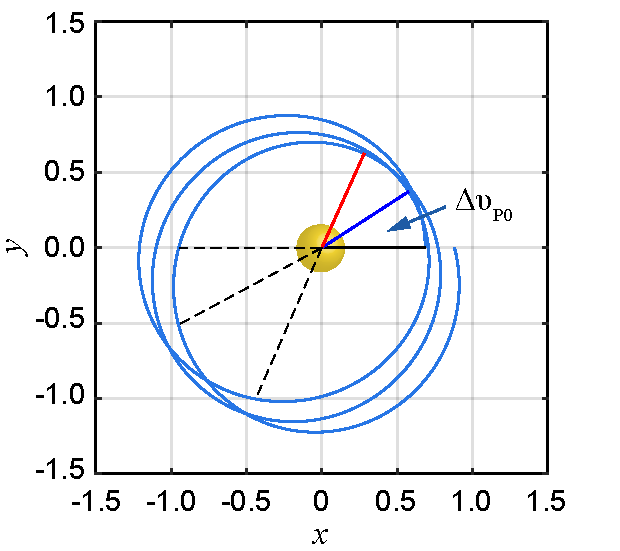
\includegraphics[width=0.5\textwidth]{Perihel01.pdf}}
\hspace{\fill}
\rightfigure{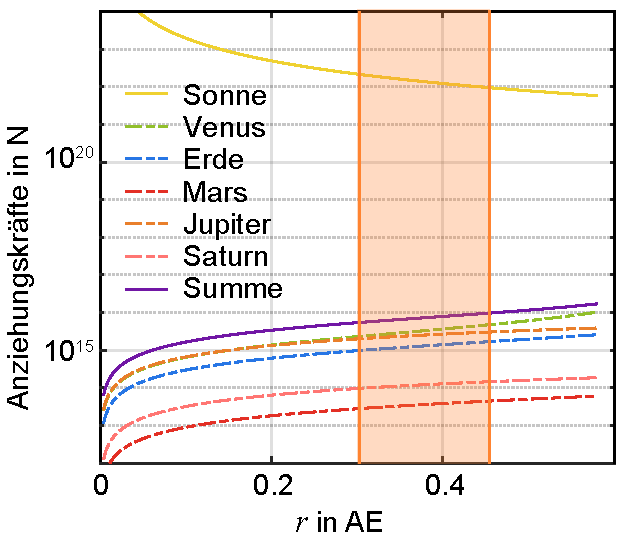
\includegraphics[width=0.5\textwidth]{StoerpotentialMerkur.pdf}}
\leftcaption{Periheldrehung.}\label{abb:hm_perihel_01}
\rightcaption[Anziehungskr�fte auf den Merkur durch die Sonne und �u�ere Planeten.]{Anziehungskr�fte auf den Merkur durch die Sonne und die �u�eren Planeten. Schattiert ist der Aufenthaltsbereich des Merkurs gezeigt. Man beachte die Gr��enunterschiede im Betrag von Sonne zu Planeten von $\approx \SI{1e6}{}$.}\label{abb:hm_stoerpotential_merkur}
\end{minipage}
\end{figure}

Aus \eqref{eq:hm_upsilon_P0} erkennen wir, dass $\upsilon_{\text{P}_0}$ nach einer Periode nur dann gleich $2\pi$ ist, wenn 
\begin{equation}
\gamma = 3+a\,\frac{b'(a)}{b(a)} \equiv 1 \,. \label{eq:hm_perihel_bed}
\end{equation}
F�r die Newtonsche Gravitationskraft $\mu{_\text{G}}/a^2$ (normiert auf die Masse $m$) ist $b(a)\!=\!-1/a^2$ und $b'(a)\!=\!2/a^3$. F�r diesen Fall folgt dann
\begin{equation*}
3+a\lk \frac{2}{a^3}\rk \lk-\frac{a^2}{1} \rk = 1 \,
\end{equation*}
und damit keine Perihelverschiebung. F�r jedes von $r^{-2}$ abweichende Kraftfeld ergibt die linke Seite von \eqref{eq:hm_perihel_bed} einen Wert $\neq\! 1$ und damit nach \eqref{eq:hm_upsilon_P0} mit $\upsilon_{\text{P}_0}\!\neq\!2\pi$ (\probref{hm_potential_merkur}) eine nicht mehr vollst�ndig geschlossene Bahn.
So ist \zb das Perihel nach einem vollen Umlauf nicht mehr bei der gleichen Anomalie zu finden.
Es hat sich etwas verschoben \bzw verdreht, ebenso wie die Apsidenlinie (\figref{hm_perihel_01}).\footnote{Wir haben die Stabilit�tsbedingung \eqref{eq:hm_stab_bedingung} und auch die Beziehung f�r die Perihelverschiebung \eqref{eq:hm_upsilon_P0} auf Basis ann�hernd kreisf�rmiger Bahnen abgeleitet \cite{Price1979}.
Sie gelten aber im Prinzip genauso f�r elliptische Bahnen. Wir verweisen hierzu auf \cite{Davies1983}.} 

\subsubsection{Berechnung des St�rpotentials und der Periheldrehung f�r den Planeten Merkur\, ($\mercury$)}\index{St�rpotential} \label{kap:Stoerpotential_Merkur}
Die Frage ist nun, wie solche Zusatzpotentiale $\Delta U_i(r)$ in der Realit�t beschaffen sind und ob man eine solche Verschiebung des Perihels berechnen und messen kann.
Wir m�chten mit einem einfachen physikalischen Modell das St�rpotential f�r den Merkur berechnen.
F�r diesen muss sich das gr��te St�rpotential ergeben, da alle anderen Planeten au�erhalb seiner Bahn liegen und damit der Anziehung des Merkurs durch die Sonne entgegen wirken.
Unser Modell f�r das St�rpotential \cite{Price1979, Davies1983} beruht auf der Annahme, dass die zeitlich gemittelten St�rungen der anderen Planeten auf den Merkur jeweils durch das Potential eines massebeladenen Rings mit Radius $a_k$ der jeweiligen Planetenbahn und der Ring-Massendichte $\rho_k=m_k/{2\pi a_k}$ mit $k=2 \ldots 8$ gegeben ist.
Hier ist $m_k$ die Masse des $k$-ten Planeten, wobei man aber wegen der verschwindenden Beitr�ge von Uranus und Neptun nur bis $k\!=\!6$ (also bis zum Saturn) aufsummieren muss.
Der Vorteil dieser Herangehensweise ist, dass man mit der oben abgeleiteten Beziehung \eqref{eq:hm_upsilon_P0} die Perihelverschiebung\index{Perihelverschiebung} $\Delta \upsilon_{\text{P}_0}$ n�herungsweise berechnen kann, ohne die komplexe Bewegungsgleichung explizit l�sen zu m�ssen.
Die mittleren Beschleunigungen der anderen Planeten auf den Merkur k�nnen entsprechend dieses Ringmodells nach folgender Formel aufsummiert werden (\probref{hm_potential_merkur}):
\begin{equation}
\Delta g_{\,\mercury}(r) = G \pi \sum \limits_{k=2}^{6} \lk \frac{m_k}{2\,\pi\,a_k} \rk \frac{r}{a_k^2 - r^2} \,.
\label{eq:hm_merkur_mittlere_beschl}
\end{equation}
Hierin ist $r$ der Bahnradius des Merkurs \cite{Price1979}.
Die nach diesem Modell des massebehafteten Rings berechnete Gravitationskraft der �u�eren Planeten auf den Merkur ist tats�chlich eine Zentralkraft (\figref{hm_stoerpotential_merkur}) und muss (da alle $a_k\!>\!r_{\mercury}$ sind) eine absto�ende Kraft sein, \dh sie wirkt der anziehenden Gravitationskraft der Sonne entgegen.
F�r das Potential k�nnen wir schreiben:
\begin{align}
	\Delta \,U_{\,\mercury}(r) &= -G \pi \sum \limits_{k=2}^{6} \lk \frac{m_k}{2\,\pi\,a_k^3} \rk \bigintsss \frac{r}{\lk 1 - \frac{r^2}{a_k^2}\rk}\,\D r \nonumber \\
	&= \frac{1}{2} G \pi \sum \limits_{k=2}^{6} \lk \frac{m_k}{2\,\pi\,a_k} \rk \log \lk 1- \frac{r^2}{a_k^2} \rk \nonumber \\
	&\approx \frac{1}{2} G \pi \sum \limits_{k=2}^{6} \lk \frac{m_k}{2\,\pi\,a_k} \rk \lek \frac{r^2}{a_k^2} + \mathcal{O}\lk \frac{r^4}{a_k^4}\rk \rek \,. \label{eq:hm_merkur_mittleres_potential}
\end{align}
Setzt man in \eqref{eq:hm_merkur_mittlere_beschl} die Werte f�r $a_k, m_k$ aus Tabelle \ref{tab:hm_bahnparameter} aus dem Tabellenanhang ein und ebenso  $r\!=\!a_{\mercury}$, dann erh�lt man  f�r das Verh�ltnis der Zusatzkraft zur Anziehungskraft der Sonne
\begin{equation*}
\frac{\Delta g_{\,{\mercury}} (a_{\mercury})}{-\mu_G/a_{\mercury}^2} \:\approx \:-\frac{\pi}{m_{\astrosun}} \, a_{\mercury}^2\, 100 \:\text{kg\,m}^{-2} \approx - \SI{6e-7}{} \,.
\end{equation*}
Das ist im Verh�ltnis zur Anziehung durch die Sonne eine sehr kleine absto�ende St�rung (Man beachte die logarithmische Darstellung in \figref{hm_stoerpotential_merkur}.).
Wir werden aber gleich sehen, welche doch messbare Wirkung dieses geringe resultierende Potential hat und vor allem auch wissenschaftshistorisch hatte.
Wir berechnen dazu f�r die Merkurbahn die Gr��en $b(a)$ und $b'(a)$, die wir f�r \eqref{eq:hm_upsilon_P0} brauchen:
\begin{align*}
		m_{\mercury} \, b_{\mercury}(a_{\mercury}) &= \underbrace{-\frac{\mu_\text{G} \, m_{\mercury}}{a_{\mercury}^2}}_{F_0 \approx \SI{-1.31e22}{}\:\text{N}} + \underbrace{m_{\mercury} \, \Delta \,g_{\,{\mercury}} (a_{\mercury})}_{\Delta F \approx \SI{7.56e15}{} \text{N}} ~, \nonumber \\  
	m_{\mercury} \, b'_{\mercury}(a_{\mercury}) \, a_{\mercury} &= \underbrace{+\frac{2 \mu_\text{G} \, m_{\mercury}}{a_{\mercury}^2}}_{-2 \, F_0} + \underbrace{m_{\mercury} \, a_{\mercury} \, \frac{\d }{\d r} \lk \Delta \,g_{\,{\mercury}}(r) \rk \bigg|_{r=a_{\mercury}}} _{\mu_\text{G} \pi\, a_{\mercury} \, m_{\mercury} \, S(r)}  
\end{align*}
mit der Summe
\begin{equation*}
	S=S(a_{\mercury})=\sum\limits_{k=2}^{6}\lk \frac{m_k}{2\pi \, {r_k}^2} \rk \frac{{r_k}^2+{a_{\mercury}}^2}{\lk {r_k}^2-{a_{\mercury}}^2 \rk^2}\,.
\end{equation*}
Das setzen wir in \eqref{eq:hm_upsilon_P0} ein und erhalten f�r die wahre Anomalie
\begin{align}
	\upsilon_{\text{P}_0} &= 2\pi \lk {3 + \frac{-2 F_0 + G\pi \, a_{\mercury}\, m_{\mercury} \, S}{F_0+\Delta F} }\rk^{-\frac{1}{2}} \nonumber \\
	  & = 2\pi \lk {\frac{1+ 3 \frac{\Delta F}{F_0} + \frac{1}{F_0}\, G\pi \, a_{\mercury}\, m_{\mercury} \, S}{1 +\frac{\Delta F}{F_0}} }\rk^{-\frac{1}{2}} \nonumber\\
		&\approx 2\pi \lk { 1 - \frac{\Delta F}{F_0} - \frac{G\pi \, a_{\mercury}\, m_{\mercury} \, S}{2F_0} }\rk + \mathcal{O}\lk {\lk \frac{\Delta F}{F_0}\rk^2}\rk \,. \label{eq:hm_mercury_perihel_shift1}
\end{align}
Mit den Daten des Merkurs $a_{\mercury}$, $m_{\mercury}$, den Werten f�r $F_0, \Delta_F$ und $S$ (siehe \mlhmref{StoerpotentialMerkur.m}), sowie der siderischen Umlaufzeit des Merkurs von 87.969 d berechnen wir f�r die Verschiebungsrate $\Delta \dot{\upsilon}_{\text{P}_0}$ des Perihels 
\begin{align}
\begin{split}
	\Delta \dot{\upsilon}_{\text{P}_0} &= \frac{\upsilon_{\text{P}_0} - 2 \pi}{T_{\mercury}}  \\
	&= \frac{\Delta \upsilon_{\text{P}_0}}{T_{\mercury}} = \frac{2 \pi}{F_0 T_{\mercury} } \, \lk{- \Delta F - \frac{1}{2} G\pi a_{\mercury} m_{\mercury} S}\rk \approx 531.5''/\text{Jh.} 
\end{split} \label{eq:hm_mercury_per_shift2}
\end{align}
Das Ergebnis der Berechnung der Potentialanteile der einzelnen Planeten ist in \mlhmref{StoerpotentialMerkur.m} ausgef�hrt und in \figref{hm_stoerpotential_merkur} dargestellt.\\
Wir haben mit relativ einfachen �berlegungen eine gute Absch�tzung f�r die Perihelverschiebung f�r ann�hernd kreisf�rmige Bahnen erhalten.\footnote{Unsere Betrachtungen zur Absch�tzung der Perihelverschiebung beruhten auf der N�herungsannahme kreisf�rmiger Bahnen \cite{Price1979, Stump1988}.
In \cite{Davies1983} und \cite{Stewart2005} wird eine Erweiterung auf elliptische Bahnen angegeben.
Der Effekt ist aber relativ klein ($<\! 1''$).
Unsere N�herung war also gerechtfertigt.} Es w�re aber doch sch�n, wenn wir auch die Bahn explizit als Funktion der Zeit berechnen k�nnten. Das wollen wir in \probref{hm_perihel_kappa3} tun.\\


\subsubsection{Bahnberechnung f�r ein verallgemeinertes Zentralkraftfeld}\index{Zentralkraftfeld} \label{kap:Allg_ZK__Merkur}
Mit \eqref{eq:hm_merkur_mittleres_potential} haben wir das St�rpotential (\bzw Kraftfeld) f�r den Merkur in einer Form bestimmt, die leider keine direkte Integration der Bewegungsgleichung erlaubt.
Man ist also auf St�rungsrechnungen angewiesen.
Wir wollen aber zun�chst f�r Potentiale, die sich als Reihenentwicklung von $r^{-n}$ darstellen lassen, einen analytischen Ansatz versuchen.
Wir schreiben dazu \eqref{eq:hm_bwg_allg_ZK} in folgender Form:
\begin{align}
	U_\text{\,ZK}(r) &= -\frac{\mu_\text{G}}{r} + \Delta U_2 + \Delta U_3 = -\frac{\mu_\text{G}}{r}  + \frac{\kappa_2}{r^2} + \frac{\kappa_3}{r^3} + \ldots \,.
	\label{eq:hm_allg_ZK_1}
\end{align}
Die spezifische, wiederum auf die Masse $m$ normierte Gesamtenergie des Systems $H$ in Polarkoordinaten ist dann mit \eqref{eq:hm_bewgl1} gegeben durch
\begin{equation}
	H = \frac{1}{2} (\dot{r}^2 + r^2\dot{\upsilon}^2) + U(r) \,. \label{eq:hm_total_energy}
\end{equation}
Mit dem Drehimpuls $L = r^2\dot{\upsilon}$ aus \eqref{eq:hm_drehimp_z} schreiben wir $\dot{\upsilon}\!=\!L/r^2$ und setzen das in die Gleichung f�r die Energie \eqref{eq:hm_total_energy} ein:
\begin{align}
  H &= \frac{1}{2} \dot{r}^2 + \frac{r^2}{2} \frac{L^2}{r^4} + U(r)
      \qquad \Rightarrow \qquad
      \dot{r}^2 = 2H - 2 \underbrace{\lk \frac{L^2}{2 r^2} + U(r) \rk}_{U_\text{eff}} \nonumber \\
\Rightarrow \dot{r} &= \sqrt{2 H - 2 \lk \underbrace{-\frac{\mu_\text{G}}{r} + \frac{L^2}{2r^2}}_{U_\text{eff, K}} + \underbrace{\frac{\kappa_2}{r^2}}_{\Delta U_1} + \underbrace{\frac{\kappa_3}{r^3}}_{\Delta U_2} \rk} ~. \label{eq:hm_allg_ZK_2}
\end{align}
Hierin sind $U_\text{eff,K}(r)$ und $U_\text{eff}(r)$ das effektive Potential des Keplerproblems \bzw des allgemeinen ZK-Feldes, wobei
\begin{equation*}
U_\text{eff,K}(r)\!=\! -\frac{\mu_\text{G}}{r} + \frac{L^2}{2r^2} ~ \;~\text{und}\;~ U_\text{eff}(r) = U_\text{eff,K}(r) + \Delta U_2 + \Delta U_3 ~~   \,.
\end{equation*}
Um $r(\upsilon)$, \dh die Bahn zu berechnen, schreiben wir die Zeitableitung des Bahnradius als
\begin{align*}
	\dot{r} &= \frac{\D r}{\D t} = \frac{\D r}{\D \upsilon}\frac{L}{r^2} = \sqrt{2\lk H - U_\text{eff}(r)\rk} ~,\\
\text{woraus}~~ \D \upsilon &= \frac{L\,\D r}{r^2\sqrt{2 \lk H - U_\text{eff}(r)\rk}}  ~~\text{folgt.}
\end{align*}
Jetzt substituieren wir $r\!=\!1/q$ und $\D r = -1/q^2\,\D q$ und erhalten
\begin{align*}
\D \upsilon &= -\frac{L \killA{q^2}\,\D q}{\killA{q^2} \sqrt{2H - 2U_\text{eff}(q)}} = -\frac{\D q}{\sqrt{2H/L^2 - 2 U_\text{eff}(q)/L^2}} ~. 
\end{align*}
Das ergibt dann ausgeschrieben
\begin{align}
\upsilon &= - \bigintsss{\frac{L}{\sqrt{2H + 2\mu_\text{G}\, q - \lk L^2 + 2\kappa_2 \rk q^2 - 2\kappa_3\,q^3}}\, \D q } ~. \label{eq:hm_allg_ZK_3} 
\end{align}
Dieses Integral gilt es nun zu l�sen.
Wir haben das in Beispiel \ref{bsp:perihel_kappa2} f�r das St�rpotential $\kappa_2 /r^2$ ausgef�hrt.

%BEISPIEL 8 %%%%%%%%%%%%%%%%%%%%%%%%%%%%%%%%%%%%%%%%%%%%%%%%%%%%%%%%%%%%%%%%%%%%%%%%%%%%%%%%%%
\begin{example}{Integration der Bewegungsgleichung f�r ein ZK mit St�rpotential $\kappa_2/{r^2}$}
Wir setzen in \eqref{eq:hm_allg_ZK_3} $\kappa_3\!=\!0$, sodass wir ein leicht modifiziertes Keplerproblem erhalten.
Wir erkennen, dass im Fall $\kappa_2 \neq 0$ das effektive Keplerpotential des ungest�rten Falls $U_\text{eff, K}(r)$ durch einen Korrekturfaktor $2\kappa_2/L^2$ vergr��ert wird.
Wir k�nnten daher direkt die L�sung f�r die Bahn aus dem reinen ZKP nehmen und entsprechend modifizierte Parameter verwenden.
Wir wollen aber die Bahngleichung f�r das gest�rte System noch einmal explizit herleiten, da dies sehr instruktiv ist.
Dazu nutzen wir f�r \eqref{eq:hm_allg_ZK_3} die Abk�rzungen
\begin{align*}
	\hat{A} &= \frac{2H}{L^2} < 0 ~\text{, da die Ellipsenbahn gebunden ist} ~,\\
	\hat{B} &= \frac{2\mu_\text{G}}{L^2} > 0 \,, \\
	\hat{C} &= -\lk 1+\frac{2\kappa_2}{L^2}\rk < 0 ~\text{, da laut Voraussetzung }\frac{\kappa_2}{L^2}\ll 1 \,.
\end{align*}
In Integraltafeln finden wir f�r $\hat{C}\!<\!0$ und $\Delta\!=\!4\hat{A}\hat{C} - \hat{B}^2\!<\! 0$, was in unserem Fall erf�llt ist, f�r das Integral folgende L�sung:
\begin{align}
	\int \frac{1}{\sqrt{\hat{A} + \hat{B}q + \hat{C}q^2}} \,\D q &= \frac{-1}{\sqrt{-\hat{C}}}\,\arcsin\lk\frac{2\hat{C}q + \hat{B}}{\sqrt{-\Delta}}\rk \,. \label{eq:hm_allg_ZK_4}
\end{align}
In der L�sung \eqref{eq:hm_allg_ZK_4} des Integrals setzen wir
\begin{align}
D&=\sqrt{-\Delta}\!=\sqrt{\hat{B}^2-4\hat{A} \hat{C}} =\sqrt{\frac{8H}{L^2}\lk 1+ \frac{2\kappa_2}{L^2}\rk + \frac{4\mu_\text{G}^2}{L^4}} ~, \label{eq:hm_allg_ZK_5} \\
B&\!=\hat{B} ~ \text{und} ~ \nonumber \\
 C&\!=\!\sqrt{-\hat{C}}\!=\!\sqrt{1+2\kappa_2/L^2} \approx 1+\kappa_2/L^2~ . \nonumber 
\end{align}
Damit folgt 
\begin{align*}
	\upsilon-\upsilon_0 &= \frac{1}{C}\,\arcsin\lk \frac{B-2C^2 q}{D}\rk \bigg|^{q(\upsilon)}_{q_0} = \frac{1}{C}\,\arcsin\lk \frac{B-2C^2 \frac{1}{r}}{D}\rk \bigg|_{r_0}^{r(\upsilon)} \\
											&= \frac{1}{C}\,\arcsin \lk \frac{B-\frac{2C^2}{r}}{D} \rk - \underbrace{\frac{1}{C}\,\arcsin \lk \frac{B-\frac{2C^2}{r_0}}{D} \rk}_{\equiv K_0/C} ~~
\end{align*}
und umgeformt
\begin{equation*}
\sin\lek C(\upsilon-\upsilon_0) + K_0\rek	= \frac{B-\frac{2C^2}{r(\upsilon)}}{D} \,.  
\end{equation*}
Das ist schon eine Gleichung f�r die Bahn, allerdings noch eine implizite.
Wir wollen $r(\upsilon)$ explizit gewinnen und formen die Gleichung deshalb weiter um zu
\begin{equation*}
	r(\upsilon) = \frac{\frac{2C^2}{B}}{1-\frac{D}{B}\sin \lek C(\upsilon-\upsilon_0) + K_0\rek} ~. 
\end{equation*}
Wir w�hlen die Integrationskonstante $K_0$ ohne Beschr�nkung der Allgemeinheit so, dass sich 
\begin{equation*}
C\upsilon_0 - K_0 = \frac{\pi}{2} 
\end{equation*}
ergibt, denn dann ist $\sin\lk C \upsilon - C \upsilon_0 + K_0 \rk  = -\cos \lk C \upsilon \rk$, womit  wir schlie�lich erhalten:
\begin{equation}
	r(\upsilon) = \frac{\frac{2C^2}{B}}{1+\frac{D}{B}\,\cos(C\upsilon)} ~. \label{eq:hm_allg_ZK_6} 
\end{equation}
\label{bsp:perihel_kappa2}
\end{example}
%BEISPIEL %%%%%%%%%%%%%%%%%%%%%%%%%%%%%%%%%%%%%%%%%%%%%%%%%%%%%%%%%%%%%%%%%%%%%%%%%%%%%%%%%%

Schreiben wir \eqref{eq:hm_allg_ZK_6} aus dem Beispiel mit 
\begin{equation*}
C=\sqrt{1+2\kappa_2/L^2} \approx 1+ \frac{\kappa_2}{L^2} ~~
\end{equation*}
und unter Umbenennung der Parameter 
\begin{align*}
\frac{2C^2}{B} &= \hat{p} = \frac{L^2}{\mu_\text{G}} \lk {1+ \frac{2\kappa_2}{L^2}} \rk = p \lk {1+ \frac{2\kappa_2}{L^2}} \rk \,,\\
\frac{D}{B} &= \hat{e} = \sqrt{1 + \frac{2H L^2}{\mu_\text{G}^2} \lk 1 + \frac{2\kappa_2}{L^2} \rk} = e \sqrt{ 1 + \frac{4H\kappa_2}{\mu_\text{G}^2 e^2}}\,,
\end{align*} 
erhalten wir schlie�lich 
\begin{equation}
	r(\upsilon) = \frac{2C^2/B}{1+\frac{D}{B}\,\cos(C\upsilon)}=\frac{\hat{p}}{1+\hat{e}\cos(C\upsilon)} ~. \label{eq:hm_allg_ZK_7}
\end{equation}
Gleichung \eqref{eq:hm_allg_ZK_7} sieht genauso aus wie die Bahngleichung f�r die Ellipse im Keplerfall \eqref{eq:hm_kegelschnitt}, allerdings mit modifizierten Parametern.
Wir erkennen, wie nicht anders zu erwarten war, dass f�r $\kappa_2 \rightarrow 0$ die Werte in die bekannten Werte f�r das reine Keplerproblem �bergehen.
Beides ist nicht verwunderlich, da durch den $\kappa_2/r^2$-Term im Potential ja nur die Gr��e des effektiven Potentials ver�ndert wird, nicht aber die $r$-Abh�ngigkeit des Gesamtpotentials.
Durch den Zusatzterm wird quasi ein \anf{effektiver Drehimpuls} des Systems erzeugt.
Man sieht aber anhand von \eqref{eq:hm_allg_ZK_6}, dass durch diesen effektiven Drehimpuls der Term mit $\cos(C\upsilon)$ nicht mehr $2\pi$-periodisch bez�glich $\upsilon$ ist, $r(\upsilon)$ ist minimal f�r $\upsilon_{\text{P}_0}\!=\!0$ (Perihel) und maximal f�r $\upsilon_{\text{Ap}}\!=\!C /\pi$ (Aphel).
In einem Zeitintervall, das dann einem vollen Umlauf entspricht, nimmt also die wahre Anomalie um $2\pi/C$ zu.\footnote{Eigentlich m�sste man zeigen, dass die siderische Umlaufzeit f�r die gest�rte Keplerellipse gleich der des ungest�rten Falls ist. Das ist aber leicht einsichtig, da wegen der Drehimpulserhaltung auch im allgemeinen ZK-Feld weiterhin der Fl�chensatz gilt.}
Die Perihelverschiebung ergibt sich mit \eqref{eq:hm_allg_ZK_7} demnach zu 
\begin{equation}
\Delta \upsilon_{\text{P}_0} = 2\pi/C  - 2\pi=  2\pi \lk \frac{1}{\sqrt{1+2\kappa_2/L^2}} -1 \rk \approx -2\pi \frac{\kappa_2}{L^2} ~. 
\label{eq:hm_allg_ZK_8}
\end{equation}
Es ist interessant, dass die Perihel-�nderung umso kleiner ist, je gr��er der Drehimpuls ist.
Das ist aber einsichtig, denn die relative �nderung des effektiven Potentials gegen�ber dem reinen Keplerproblem ist bei gro�em Drehimpuls entsprechend kleiner.
Wir zeigen in \figref{hm_simulationen_merkur1} verschiedene mit \mlhmref{PerihelKappa2.m} berechnete Simulationen von Bahnkurven f�r ein Potential mit Zusatzterm $\kappa_2\!\neq\! 0$, wobei die Parameter bewusst unrealistisch gro� gew�hlt wurden, um die Effekte deutlich sichtbar zu machen. 

\begin{figure}
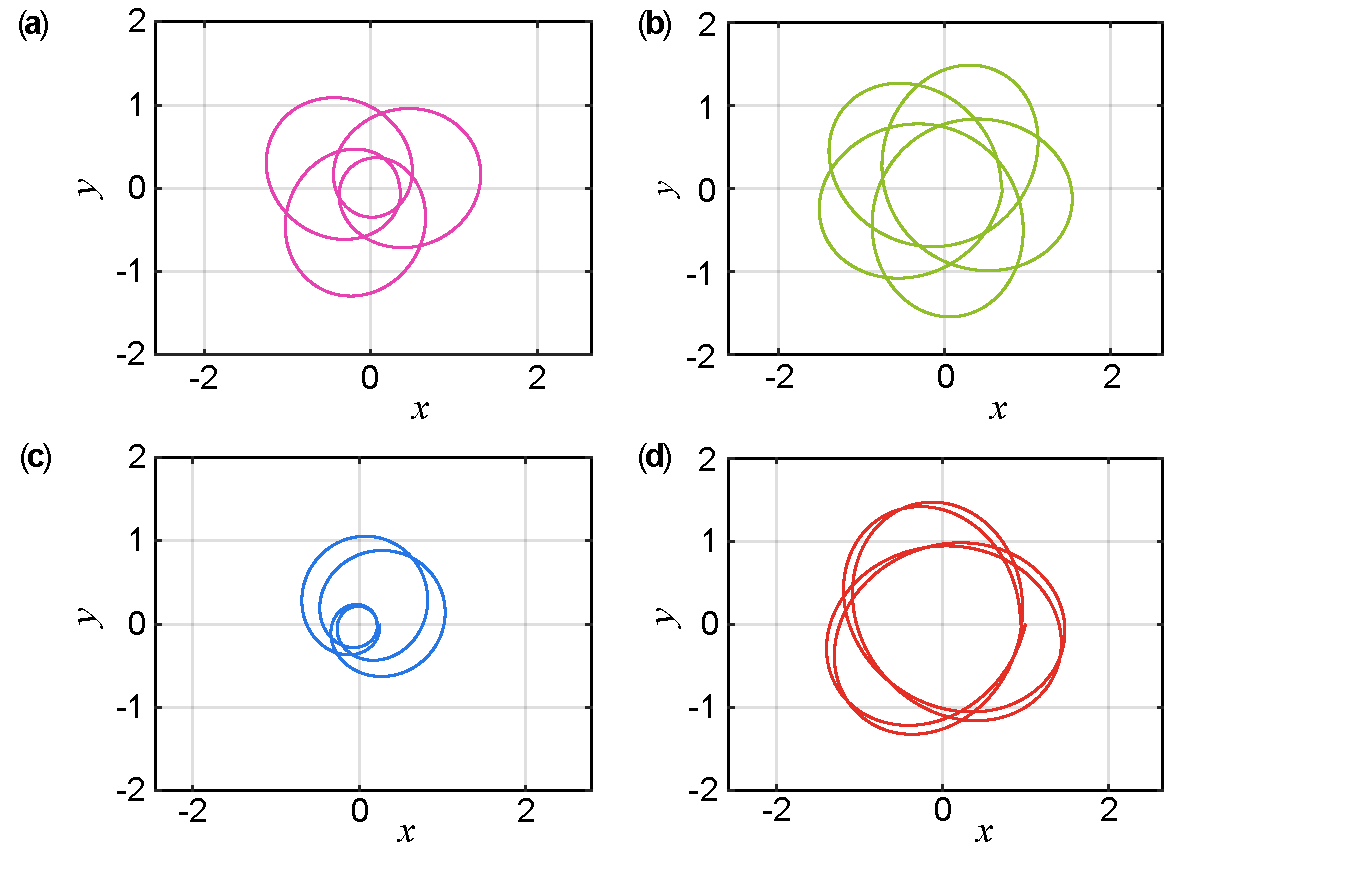
\includegraphics[width=\textwidth]{simulation_merkur1.pdf}%
\caption[Simulation von Bahnformen f�r verschiedene Parameters�tze.]{Simulation von Bahnformen f�r verschiedene Parameters�tze des Zentralkraftfeldes. Die Parameter sind $e=0.5, a = 1 $ und $\kappa_2 = -0.1\, \mu_\text{G}, + 0.1\, \mu_\text{G}, -0.2\, \mu_\text{G} \:\text{und}\: +0.2\,\mu_\text{G}$ f�r die Bilder \fa bis \fd. Um die Effekte deutlich sichtbar zu machen, wurden die Parameter unrealistisch gro� gew�hlt. Siehe \mscr~\mlhmref{PerihelKappa2.m}.}%
\label{abb:hm_simulationen_merkur1}%
\end{figure} 

\subsubsection{Merkur-Perihelverschiebung -- relativistischer Effekt}\index{Perihelverschiebung!relativistische} \label{kap:Relativistic_Merkur}
So sch�n und nachvollziehbar unsere Rechnungen zur Perihelverschiebung des Merkurs in \kapitel{Stoerpotential_Merkur} auch waren, die von vielen Astronomen mit Methoden der St�rungsrechnung sehr genau berechnet wurden, gibt es doch leider einen Haken.
Man fand n�mlich zwischen den berechneten ca. $531''$/Jh. und den tats�chlich beobachteten ca. $572''$/Jh. eine signifikante, nicht erkl�rbare Differenz von $41''$/Jh.
Auch der franz�sische Astronom Urbain Le Verrier\indexp{Le Verrier, Urrbain Jean Joseph}\footnote{Urbain Jean Joseph Le Verrier (1811--1877) war ein franz�sischer Astronom und Mathematiker. Ihm gelang 1846 die Vorausberechnung der vermutlichen Bahn des bis dahin unentdeckten Planeten Neptun aus den Bahnst�rungen des Uranus. Der Neptun wurde dann an der Berliner Sternwarte durch den Astronomen Galle mit dem 22-Zentimeter-Fraunhofer-Refraktor auch an der von Le Verrier vorhergesagten Position gefunden. Le Verrier gilt im �brigen auch als Erfinder der Wetterkarte.}, dessen genaue Berechnungen die Entdeckung des Neptuns erm�glicht hatten, konnte diese Diskrepanz nicht erkl�ren.
Er schlug vor, sicherlich durch den Erfolg beim Neptun ermutigt, nach einem inneren Planeten zu suchen.
Dieser erhielt den Namen Vulkan\footnote{Offensichtlich ein Vorgriff auf \emph{StarTrek}.}, er blieb allerdings im Gegensatz zum Neptun unauffindbar.
Die L�sung dieses R�tsels gelang erst Einstein\indexp{Einstein, Albert}\footnote{Albert Einstein (1879--1955) war einer der bedeutendsten Physiker der Weltgeschichte. Seine Forschungen zu Raum und Zeit,  sowie zum Wesen der Gravitation haben unser modernes Weltbild ma�geblich gepr�gt und seit Newton die wohl gr��te Revolution in der Physik eingeleitet.} mit seiner Arbeit zur \anf{Erkl�rung der Perihelbewegung des Merkur aus der allgemeinen Relativit�tstheorie} \cite{Einstein1915}.
Wir k�nnen hier leider nicht die Theorie darstellen.
Deshalb verweisen wir auf die entsprechenden Lehrb�cher \cite{Stephani1991, Moore2013}, k�nnen aber angeben, dass auf Basis der Allgemeinen Relativit�tstheorie die Bewegung eines K�rpers in einem ZKF durch folgende Bewegungsgleichung beschrieben werden kann: 
\begin{align}
\begin{split}
	\ddot{r} &=  -\frac{\mu_\text{G}}{r^2} + \lk 1- \frac{3\mu_\text{G}}{c^2 r} \rk \frac{L^2}{r^3} = -\frac{\mu_\text{G}}{r^2} + \frac{L^2}{r^3} - \frac{3\mu_\text{G} L^2}{c^2 r^4} \\
	&= -\frac{\mu_\text{G}}{r^2} + \frac{L^2}{r^3} - \frac{\d}{\d r} \Delta U_\text{rel}(r) 
\end{split} \label{eq:hm_einstein_01} 
\end{align}
mit $ \Delta U_\text{rel}(r) = -\mu_\text{G} L^2/(c^2 r^3) $. 
Die Bewegungsgleichung \eqref{eq:hm_einstein_01} wird in \probref{hm_perihel_kappa3} gel�st.
Hier wollen wir in der N�herung nahezu kreisf�rmiger Bahnen die Gr��e der Perihelverschiebung durch den relativistischen Effekt absch�tzen.
Wir benutzen die Beziehung \eqref{eq:hm_upsilon_P0}, die unter der Annahme kleiner St�rungen hergeleitet wurde. 
Wir berechnen $b(a)$, $b'(a)$ f�r den relativistischen Fall, nutzen $L_{\mercury} \approx \mu_{\text{G}} a_{\mercury}$ aus \eqref{eq:hm_drehimpuls_von_ae} und erhalten f�r $\gamma$ aus \eqref{eq:hm_upsilon_P0}
\begin{align*}
\gamma &= \sqrt{\frac{1+\frac{3 \kappa_3}{a^2 \mu_\text{G}}} {1-\frac{3 \kappa_3}{a^2 \mu_\text{G}}}} \,, 
\end{align*}
woraus wir erhalten:
\begin{subequations}
\begin{align}
\Delta \upsilon_{\text{P}_0},\text{rel} = 2\pi \lk \frac{1}{\gamma} -1 \rk \approx -6 \pi \frac{\kappa_3}{a^2 \mu_\text{G}} \,~~\text{und} \\
\Delta \dot{\upsilon}_{{\text{P}_0},\text{rel}} = \frac{6 \pi}{c^2} \frac{\mu_{\text{G}}}{a} \frac{1}{T_{\,\mercury}} \approx 41.3''/\text{Jh.} \, 
\end{align} \label{eq:hm_rel_perihel_val}
\end{subequations} 
Die st�rungstheoretische Rechnung (siehe auch \probref{hm_perihel_kappa3}) ergibt unter Ber�cksichtigung der Elliptizit�t einen kleinen Korrekturfaktor $(1-e^2)$:
\begin{equation}
\Delta \dot{\upsilon}_{{\text{P}_0},\text{rel}} = \frac{6 \pi}{c^2} \frac{\mu_{\text{G}}}{a(1-e^2)} \frac{1}{T_{\,\mercury}} \approx 43''/\text{Jh.} \label{eq:hm_rel_perihel_val2}
\end{equation}
Da wir f�r die Berechnung sowohl von \eqref{eq:hm_rel_perihel_val} als auch \eqref{eq:hm_mercury_per_shift2} kleine St�rungen und damit eine m�gliche Linearisierung der Bewegungsgleichung vorausgesetzt haben, k�nnen wir die Verschiebungen aus den Rechnungen \eqref{eq:hm_mercury_per_shift2} und \eqref{eq:hm_rel_perihel_val2} addieren.
Die Summe ergibt ca. $573''/$Jh., was sehr gut mit den experimentellen Befunden �bereinstimmt.
Einstein\indexp{Einstein, Albert} bekam, nachdem er diese Berechnungen 1915 durchgef�hrt hatte, wie er selber angab, \anf{Herzrasen} und war \anf{einige Tage au�er sich vor Freude}.
Irgendwie kann man dies auch 100 Jahre sp�ter noch gut nachf�hlen.

\begin{figure}
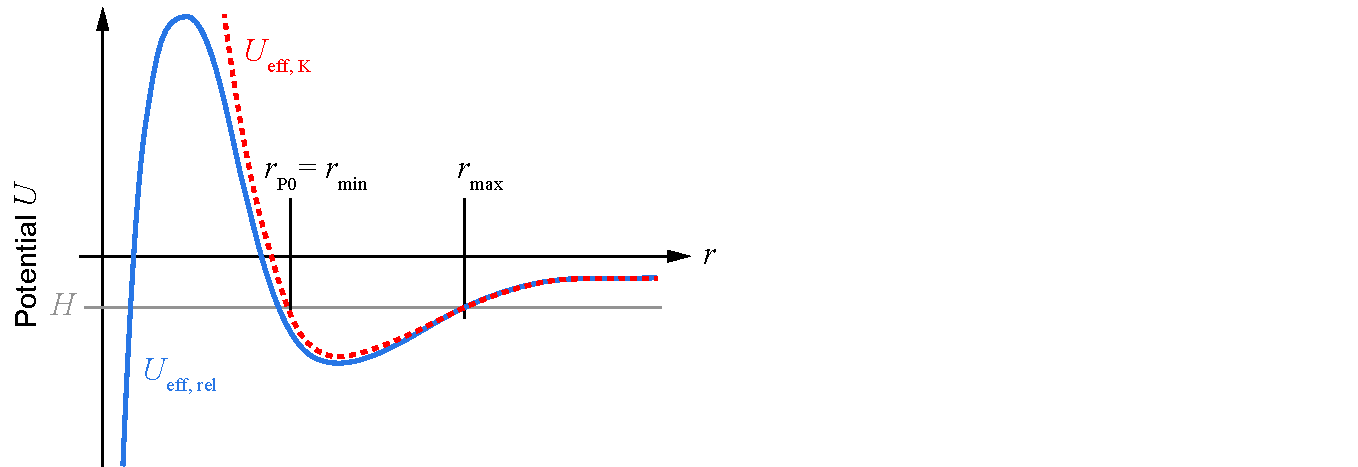
\includegraphics[width=\textwidth]{RelativisticPotential.pdf}%
\caption[Potential unter Ber�cksichtigung der relativistischen Korrektur.]{Darstellung des Potentials um einen Stern unter Ber�cksichtigung der relativistischen Korrektur, wobei $U_\text{eff,K}\!=\!-\mu_\text{G}/r + L^2/(2r^2)$ und $U_\text{eff,rel}\!=\!U_\text{eff,K}-\mu_\text{G}L^2/(c^2r^3)$. Die relativistische Korrektur ist im Bild stark �berh�ht dargestellt.}%
\label{abb:hm_relativistic_merkur}%
\end{figure} 
Wir wollen jetzt noch eine anschauliche Erkl�rung der relativistischen Perihelverschiebung geben.
Wir betrachten dazu \figref{hm_relativistic_merkur}, in der wir das effektive Potential ohne und mit stark �berh�hter relativistische Korrektur dargestellt haben.
Im nicht-relativistischen Fall ergibt das effektive Potential eine Senke, in der bei einer Energie $H\!<\!0$ der K�rper zwischen $r_\text{min}\!=\!r_{\text{P}_0}$ und $r_\text{max}$ seine Bahn hat.
Durch das relativistische Potential -- welches man sich als ein Ergebnis der Raumkr�mmung um die Zentralmasse herum vorstellen kann -- wird aber das effektive Potential bei kleinen $r$ (man beachte die $r^{-4}$-Abh�ngigkeit) so beeinflusst, dass der umlaufende K�rper bei gleicher Energie dem Zentralk�rper n�herkommt.
Da dort die Bahngeschwindigkeit am gr��ten ist, wird der Planet in gleicher Zeit einen etwas gr��eren Abschnitt der Bahn zur�cklegen.
Folglich hat er, wenn er zu seinem definierten Ausgangspunkt (\zb dem Perihel) zur�ckkommt, einen Winkel $>\! 2\pi$ �berstrichen.

In \probref{hm_perihel_kappa3} berechnen wir die Bahn f�r Potentiale mit beliebigem $\kappa_3$-Term.
Aus der Rechnung erh�lt man neben der schon abgesch�tzten Perihelverschiebung auch die zeitliche Entwicklung des Bahnradius als Funktion der wahren Anomalie $r(\upsilon(t))$.
Dieser zeigt durch das St�rpotential bedingt Oszillationen, wie wir sie bei der Betrachtung der Stabilit�t von Planetenbahnen bereits abgesch�tzt haben. F�r interessierte Leser sei auf eine sch�ne einfache linearisierte Berechnung der Merkurpr�zessions f�r den relativistischen Fall in Ref. \cite{Hall2022} verwiesen, die ebenfalls f�r ein nichtrelativistisches $\kappa_3/r^3$ St�rpotential verwendet werden kann.

\subsection{Kometen}\index{Kometen}\label{kap:kometen}
Kometen oder Schweifsterne sind faszinierende Himmelsk�rper.\footnote{Eine sehr lesenswerte und ausgesprochen ansprechend gestaltete �bersichten zu Kometen findet sich in \cite{Stump1988}.} Vermutlich sind sie nahezu unver�nderte Restmaterie aus der Entstehungszeit unseres Sonnensystems.
Die meisten Kometen werden aus ihren urspr�nglichen Bahnen durch Gravitationskr�fte und Kollisionen untereinander abgelenkt und auf langgestreckte Ellipsenbahnen geschickt.
Ein Komet besitzt einen Kern aus Staub und Eisk�rnern, der bei ausreichender Sonneneinstrahlung eine Gash�lle (Koma) und einen Schweif ausbildet.
Die L�nge des Schweifs kann mehrere hundert Millionen Kilometer erreichen.
Ber�hmte Kometen sind \zb der gro�e Komet von 1680, der am Tageshimmel zu sehen war, der Komet Donati von 1858, der als sch�nster Komet aller Zeiten gilt, und nat�rlich der ber�hmte Halleysche Komet.
Einigen Menschen ist es sogar verg�nnt, den Halleyschen Kometen\index{Halleyscher Komet}\index{Komet!Halleyscher} in ihrem Leben zweimal zu sehen.
Seine Ber�hmtheit erlangte er dadurch, dass seine Wiederkehr nach der Beobachtung im Jahr 1682 von Halley f�r 1758 vorhergesagt wurde.
Halley erlebte sie selbst nicht mehr.
Aber das von ihm vorhergesagte Wiedererscheinen des Kometen wurde am 25.12.1758 von dem s�chsischen Amateurastronomen(!) Palitzsch\footnote{Johann Georg Palitzsch (1723--1788) war ein s�chsischer Landwirt, Astronom und Naturwissenschaftler. Manche Literatur beschreibt ihn als \anf{Bauernastronom}, da er seine Beobachtungen auf seinem Landgut nahe bei Dresden machte.} tats�chlich beobachtet.
Dies war ein unglaublich gro�er und deutlich sichtbarer Erfolg der Newtonschen Gravitationstheorie\indexp{Newton, Sir Isaac}, der in etwa mit der Beobachtung der Lichtablenkung von 1919 zur Best�tigung der Allgemeinen Relativit�tstheorie verglichen werden kann.
Wir wollen uns im Folgenden auf wiederkehrende Kometen mit elliptischen Bahnen konzentrieren.
Die Berechnung elliptischer Kometenbahnen ist im Prinzip der f�r Planeten �hnlich.
Bei Kometen wird zur Bahnberechnung neben der Exzentrizit�t $e$ die \gls{periheldistanz} $q$ und der Periheldurchgang $t_0$ anstelle des Bahnradius und der mittleren Anomalie (Tabelle \ref{tab:hm_parameter_kometen}) angegeben.
Allerdings sind die Exzentrizit�ten bei Kometen sehr gro� ($e\!\approx\! 1$), was zu numerischen Schwierigkeiten bei der L�sung der Kepler-Gleichung f�hrt und die Benutzung der Mittelpunktsgleichung oder der einfachen Reihenentwicklungen nicht mehr erlaubt.
Wir werden deshalb zur Berechnung der exzentrischen Anomalie ein modifiziertes Verfahren benutzen (siehe \mscre \mlhmref{KometenZeit.m} und \mlhmref{KometenObsHor.m}).
Das Prinzip besteht darin, die Ellipsenbahn durch eine parabel�hnliche Bahn zu approximieren.
Wir  k�nnen dies hier nur skizzieren und verweisen f�r mehr Details auf die ausgezeichnete Darstellung in \cite{Montenbruck1999}.
F�r $e\!>\!0.9$ und eine mittlere Anomalie nahe am Perihel ($M\!<\!0.1\degree$) definiert man f�r diese Parabel-Approximation aus der exzentrischen Anomalie die sogenannten Stumpffschen\footnote{Karl Johann Nikolaus Stumpff (1895--1970) war ein deutscher Astronom, der in Berlin, Graz und G�ttingen vor allem auf dem Gebiet der mathematischen Himmelsmechanik forschte.} Funktionen\index{Stumpffsche Funktionen}\index{Funktionen!Stumpffsche}\cite{Walter2018}.
\begin{align}
c_1(E) &= \frac{\sin E}{E} = \sum_{n=1}^{\infty} (-1)^{n+1} \frac{E^{2(n-1)}}{(2n-1)!} \,, \label{eq:hm_Stumpff_fkt} \\
c_2(E) &= \frac{1-\cos E}{E^2} = \sum_{n=1}^{\infty} (-1)^{n+1} \frac{E^{2(n-1)}}{(2n)!} \,,\nonumber \\
c_3(E) &= \frac{E-\sin E}{E^3} = \sum_{n=1}^{\infty} (-1)^{n+1} \frac{E^{2(n-1)}}{(2n+1)!} \,. \nonumber
\end{align}
Man substituiert $E$ in der Kepler-Gleichung durch $c_3(E)$ und erh�lt mit \eqref{eq:hm_mittlere_anomalie}
\begin{equation*}
(1-e) E + e\,c_3(E)\, E^3 = \sqrt{\mu_\text{G} \lk \frac{1-e}{q} \rk^3} (t-t_0)  = M(t)  \,,
\end{equation*}
woraus mit der Hilfsgr��e 
\begin{equation*}
Q(e) = \sqrt{\frac{3\,e\, c_3(E)}{1-e}} E
\end{equation*}
aus der Kepler-Gleichung eine modifizierte Barker-Gleichung\index{Gleichung!Barker-} (siehe auch \probref{hm_bwglg_hyp_parab}) wird:
\begin{equation}
Q+\frac{Q^3}{3} = \sqrt{6\,e \, c_3(E)} \sqrt{\frac{\mu_\text{G}}{2q^3}}\,(t-t_0)\,.
\label{eq:hm_Barker_glg}
\end{equation}
Diese wird nun iterativ nach $E$ mit einem Anfangswert $E_0\!=\!0$ \bzw $c_3(0)\!=\!\frac{1}{6}$ gel�st.
Die so bestimmten exzentrischen Anomalien $E_n$ ($n$ wird bestimmt durch die Genauigkeit, die man erreichen will) werden dann zur Berechnung der Stumpffschen Funktionen\index{Funktion!Stumpffsche} $c_1(E_n), c_2(E_n), c_3(E_n)$ benutzt, wobei die Reihenformeln \eqref{eq:hm_Stumpff_fkt} sehr schnell konvergieren, was die gesamte Bahnberechnung damit schnell und relativ genau macht \cite{Montenbruck1999}.
Die Bahnkoordinaten ergeben sich zu
\begin{align}
x &= r\cos\upsilon = q \lk 1 - \frac{2\,c_2(E)}{6e\,c_3(E)} \,Q^2 \rk \,, \label{eq:hm_bahn_koord_komet} \\
y &= r\sin\upsilon = 2q \lk \frac{1+e}{2e} - \frac{1}{6\, c_3(E)}\, c_1(E) \, Q\rk \,, \nonumber \\
r &= q \lk 1+ \frac{2\,c_2(E)}{6\,c_3(E)}\,Q^2\rk \,.\nonumber
\end{align}
Die weitere Rechnung entspricht den Berechnungsschritten, wie wir sie bei den Planeten kennengelernt haben.
\figref{hm_kometenbahnen1} zeigt die Berechnungen f�r vier verschiedene Kometen.
Man beachte die starken Bahnneigungen zur Ekliptik und die parabelartigen Verl�ufe f�r Kometen mit gro�en Exzentrizit�ten.
Man erkennt auch sehr sch�n die Besonderheit des Halleyschen Kometen mit seiner f�r Kometen relativ kurzen Periode von $75.3$ Jahren und seiner retrograden\index{Bahn!retrograde} Bahn, die bis zu Neptun und Pluto reicht.

\begin{figure}%
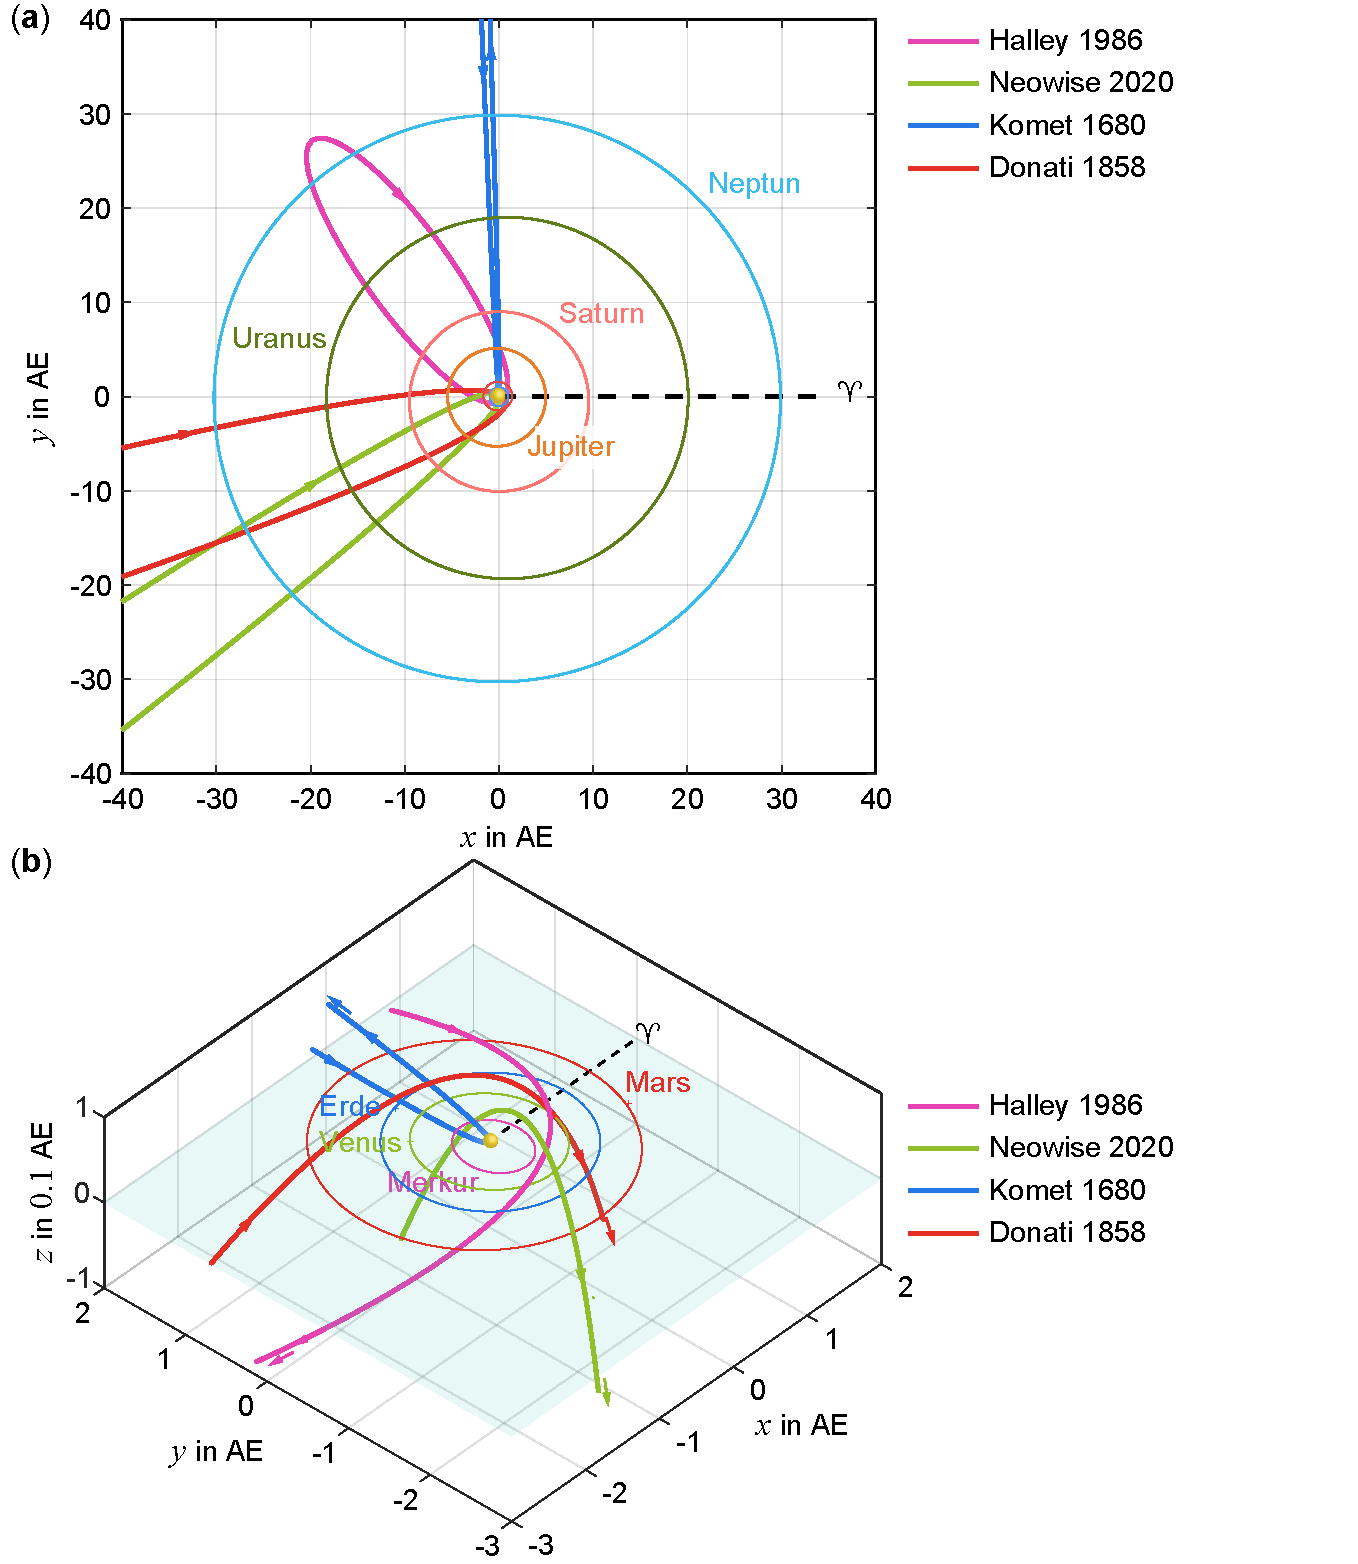
\includegraphics[width=\textwidth]{Komet1.pdf}%
\caption[Kometenbahnen im Vergleich.]{Bahnen verschiedener Kometen im Vergleich. \fa Projektion der Bahnen auf die Ekliptik. \fb 3D-Darstellung der Bahnen in Periheln�he (Sie \mscr~\mlhmref{KometenBahnen.m}).}%
\label{abb:hm_kometenbahnen1}%
\end{figure}

Wir m�chten an dieser Stelle aber noch auf einen Punkt hinweisen, der bei Berechnungen genaue Zeiten und Koordinaten f�r eine Beobachtung wichtig ist.
Bisher haben wir bei unseren Rechnungen die Lichtlaufzeit \index{Lichtlaufzeit} von den Planeten oder Kometen zum Beobachtungsort nicht ber�cksichtigt.
Die so berechneten Koordinaten hei�en deshalb auch astrometrische \index{Koordinaten!astrometrische} Koordinaten und entsprechen Beobachtungskoordinaten f�r eine angenommene Lichtgeschwindigkeit $c\rightarrow\infty$.
Bei fernen Kometen und auch Planeten ben�tigt das Licht aber f�r die Distanzen zu uns eine endliche Zeit $t_\text{L}\!\approx\!\Delta_0/c$.
W�hrend dieser Zeit bewegt sich der Himmelsk�rper weiter.
Der beobachtete Ort $\vec{r}_\text{B}$ liegt daher etwas \anf{hinter} dem Ort $\vec{r}_\text{HK}$, an dem sich der Himmelsk�rper zur Beobachtungszeit $t$ tats�chlich befindet, d.\,h. es gilt
\begin{equation}
\vec{r}_\text{B} = \vec{r}_\text{\astrosun}(t) + \lek \vec{r}_\text{HK}(t) - \dot{\vec{r}}_\text{HK}(t)\,t_\text{L}\rek \approx \vec{r}_\text{\astrosun}(t) + \lek \vec{r}_\text{HK}(t) - \dot{\vec{r}}_\text{HK}(t)\, \frac{\Delta_0}{c}\rek \,.
\label{eq:hm_scheinbare_koord_B}
\end{equation} 

Hierin sind $\vec{r}_\text{B}$ die beobachteten (scheinbaren) Koordinaten\index{Koordinaten!scheinbare}, $\vec{r}_\text{\astrosun}$ die geozentrischen Koordinaten der Sonne und $\vec{r}_\text{HK}$ die berechneten heliozentrischen (astrometrischen) Koordinaten des Himmelsk�rpers.
$\Delta_0$ ist die geometrische \gls{entfernunghimmelskoerper} und $\dot{\vec{r}}_\text{HK}$ die Bahngeschwindigkeit.
In \probref{hm_lichtlaufzeit} werden dazu einige Absch�tzungen angestellt, in \mlhmref{KometenBahnen.m} wird die im Allgemeinen kleine Korrektur bei der Berechnung der Beobachtungsdaten von Kometenbahnen ber�cksichtigt.
Bei nahen und relativ langsamen Objekten sind diese Korrekturen im Allgemeinen zu vernachl�ssigen. 
Da die Kometen auf ihrer Bahn viele St�rungen erfahren -- manchmal bleiben sie sogar unauffindbar --, unterscheiden sich die Bahnparameter von Periode zu Periode, wie man am Beispiel des  Halleyschen Kometen sehen kann, der seit einigen Jahrhunderten vermessen wird (\textbf{�bungen} \ref{prob:hm_kometen_asteroiden} und \ref{prob:hm_verweildauer_komet_erdbahn}). 

\begin{figure}%
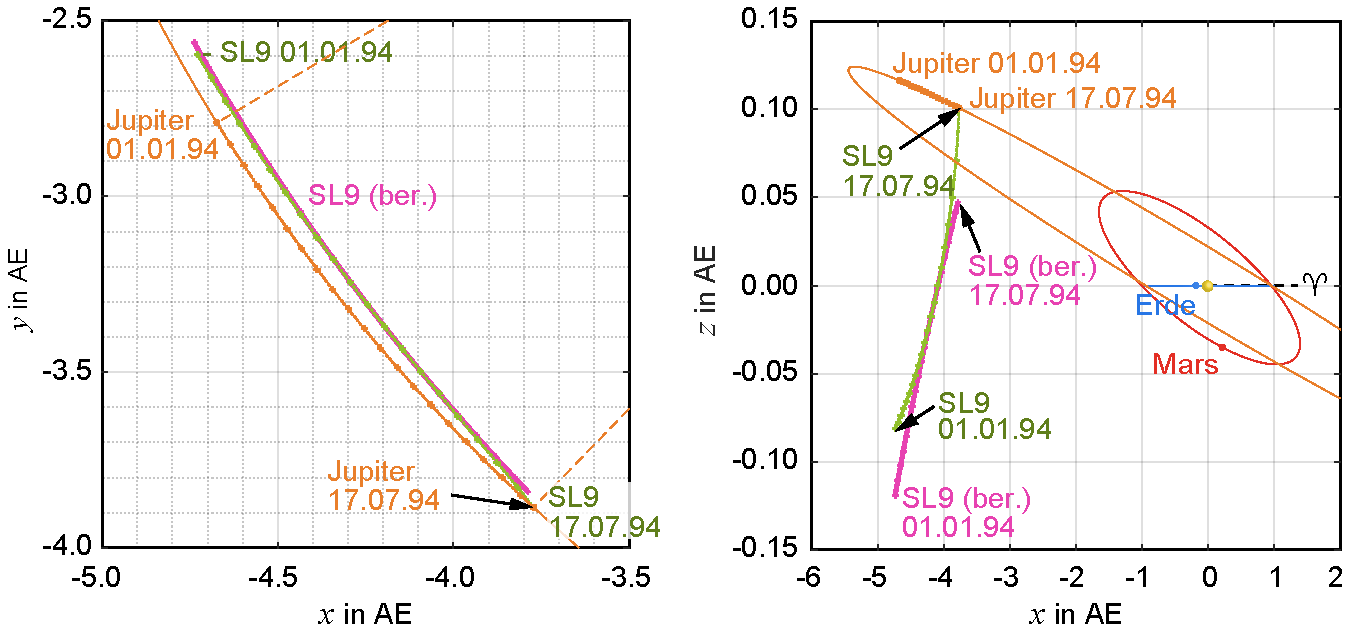
\includegraphics[width=\textwidth]{SL9.pdf}%
\caption[Shoemaker-Levy D/1993 F2.]{Shoemaker-Levy D/1993 F2 (Beispiel \ref{bsp:hm_shoemaker_levy}, \mlhmref{KometenSL9.m}). Man beachte, dass die rechte Abbildung in der $z$-Koordinate stark gestreckt ist!}%
\label{abb:hm_shoemaker_levy_komet}%
\end{figure}

Ein besonders beeindruckendes Beispiel einer Bahnver�nderung war der Komet Shoemaker-Levy.
Seine Bruchst�cke tauchten wie bereits erw�hnt im Juli 1994 in den Planeten Jupiter ein.
Wir haben bereits in \kapitel{stoerungsrechnung} die heliozentrischen Koordinaten dieses Kometen �ber numerische Integration bis zu seinem Zusammenprall mit Jupiter berechnet.
Wir vergleichen dieses Ergebnis mit der durch mittlere Bahnelemente gegebenen Keplerbahn.
Man erkennt in \figref{hm_shoemaker_levy_komet} sehr gut, dass die ungest�rte Kometenbahn durch die N�he zum Jupiter bereits 6 Monate vor dem Zusammensto� massiv beeinflusst wird.
Man kann also bereits zu diesem Zeitpunkt nicht mehr von einer ungest�rten Keplerbahn sprechen.\\
Im Juli 2020 hatten die Menschen auf der Nordhalbkugel der Erde das Gl�ck, den Kometen Neowise beobachten zu k�nnen.
Er bildete einen eindrucksvollen Schweif aus (\figref{hm_komet_neowise1}) und war mehrere Tage sehr gut nach Sonnenuntergang und vor Sonnenaufgang sichtbar.
Aus den in Tabelle \ref{tab:hm_parameter_kometen} angegebenen Werten k�nnen wir mit dem \mscr \mlhmref{KometenObsHor.m} dessen Bahn berechnen und auch erkennen, dass wir mit unserem Beobachtungsdatum gro�es Gl�ck hatten, da der Komet nur wenige Tage so gut sowohl am Abend- als auch am Morgenhimmel zu sehen war.
\begin{figure}%
\centering
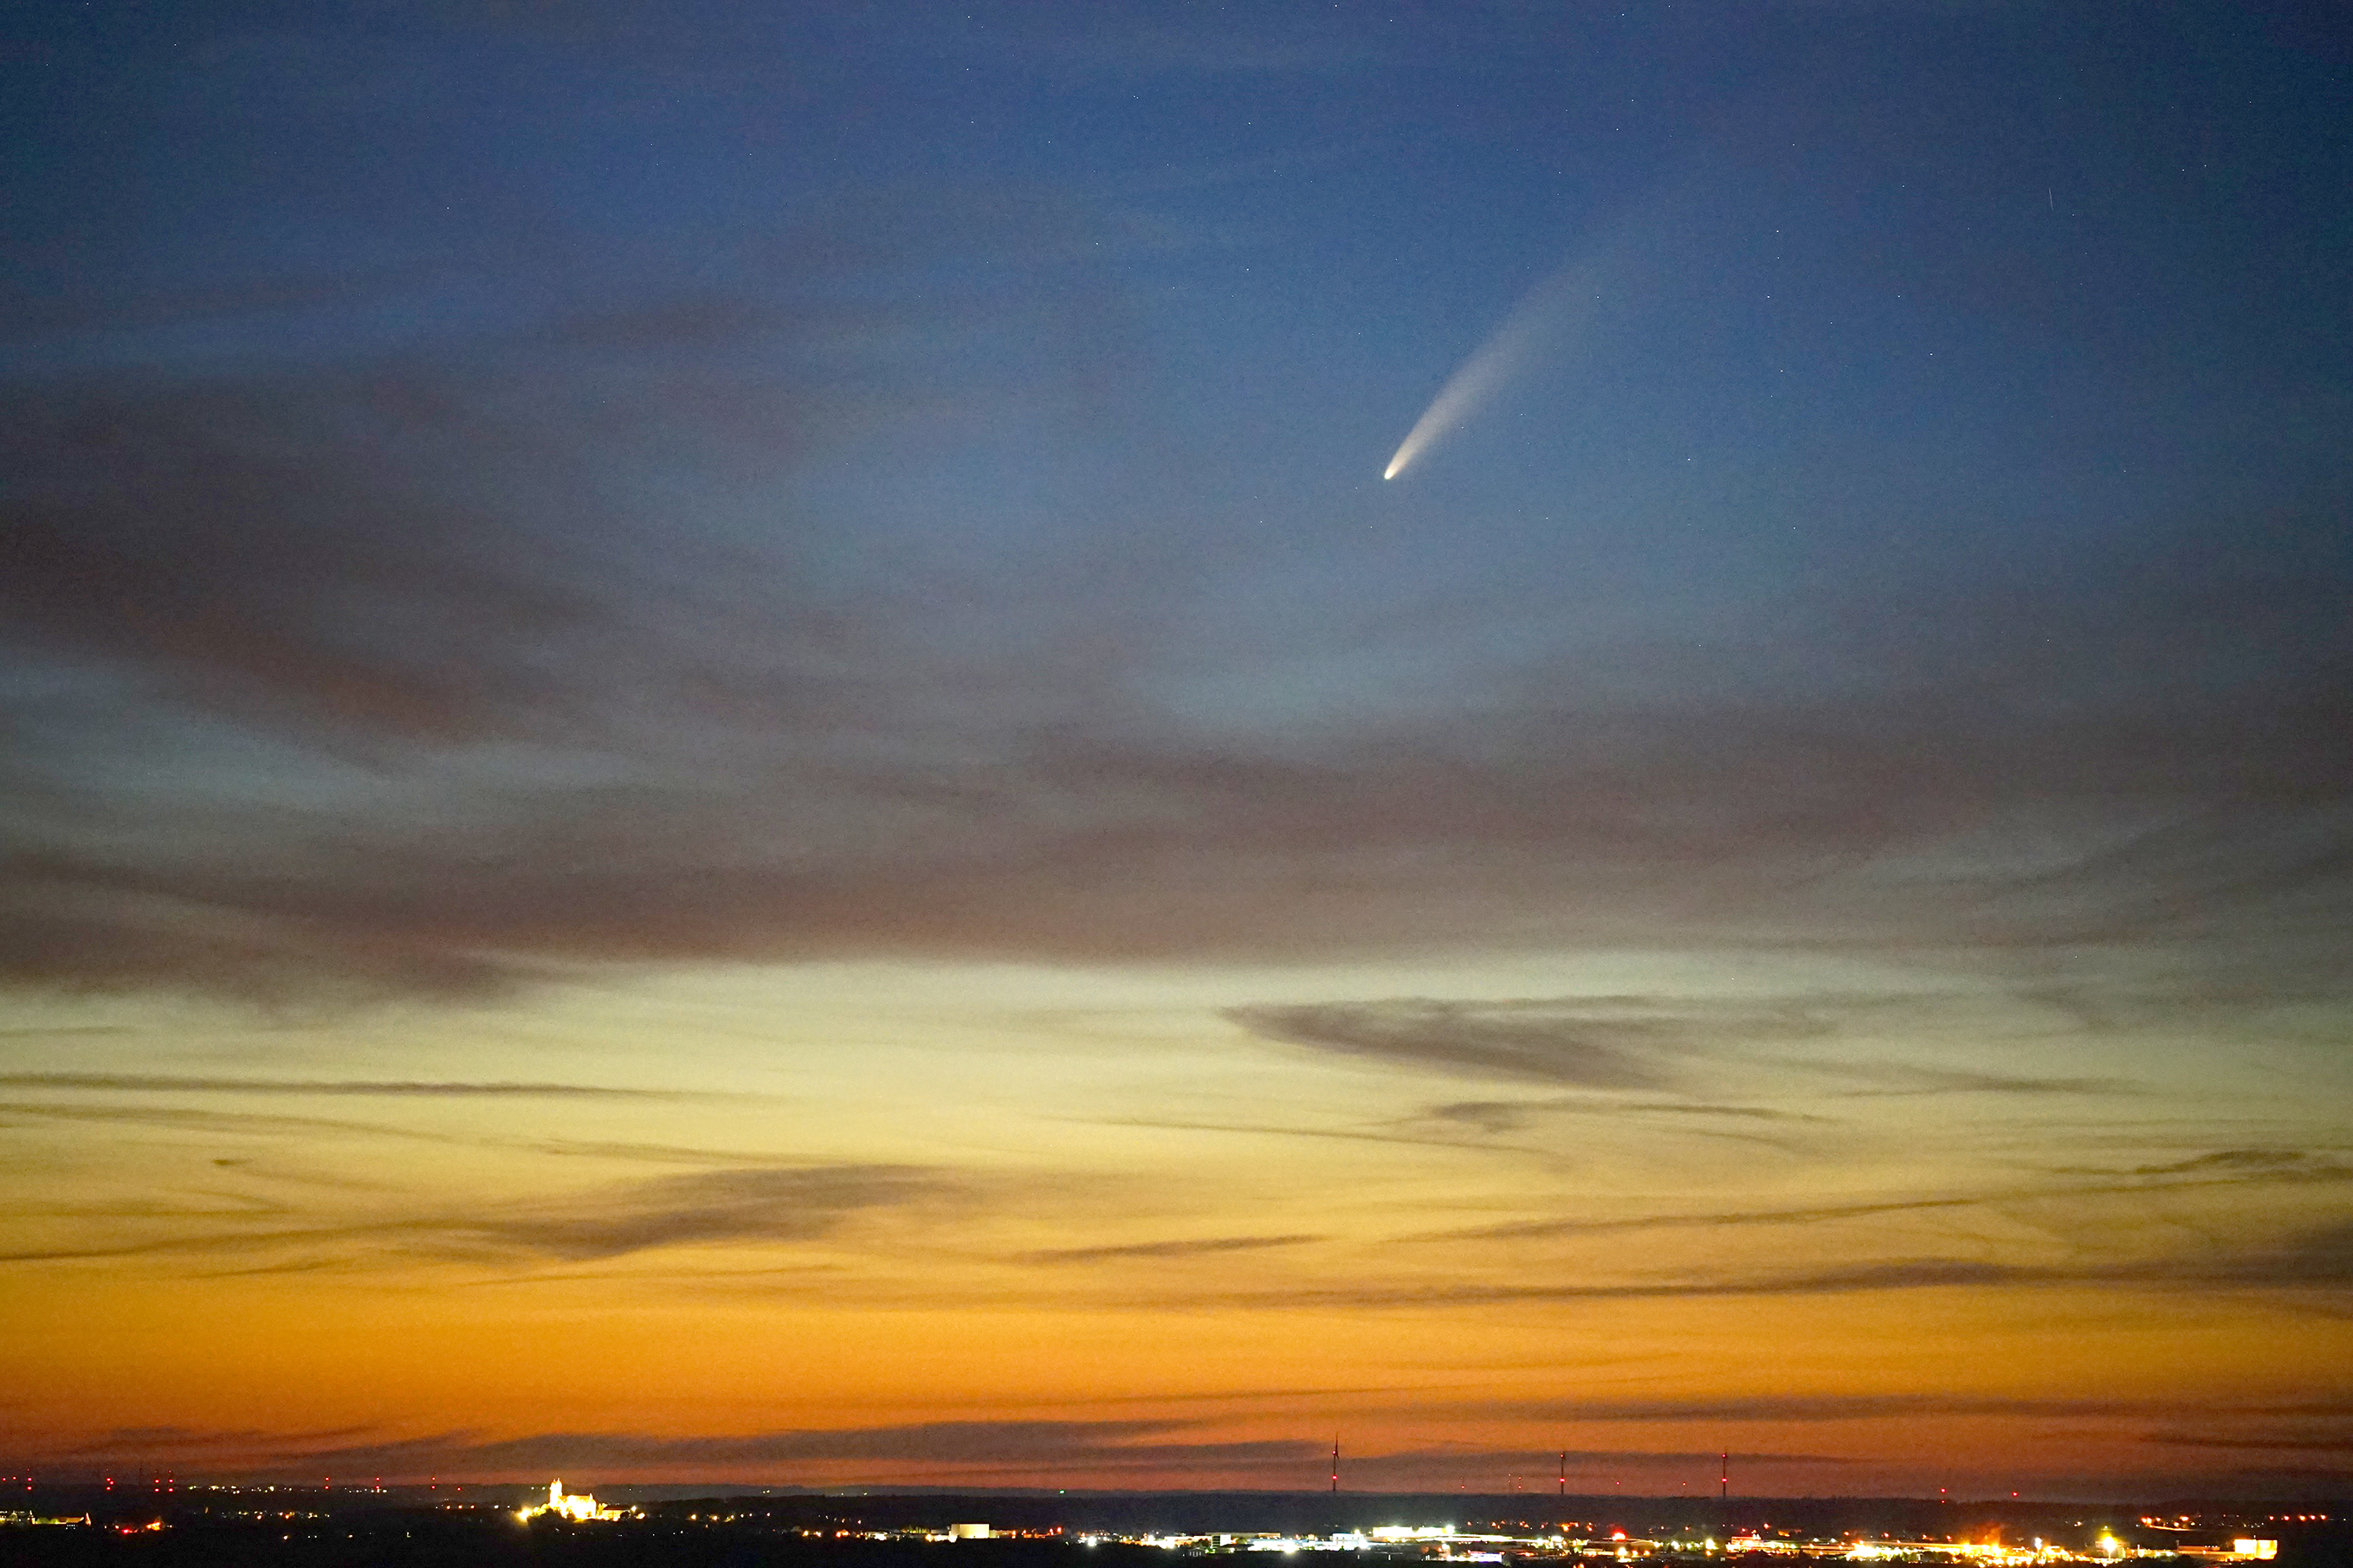
\includegraphics[width=0.75\textwidth]{KometNeowise.JPG} \\%
\caption[Beobachtung des Kometen Neowise von der Ostalb.]{Beobachtung des Kometen Neowise von der Ostalb aus ($48.8\degree$N, $10.2\degree$ O). Aufgenommen von Sylvia und Michael Kaschke am 12.07.2020, 22:30 MESZ.}%
\label{abb:hm_komet_neowise1}%
\end{figure}
\begin{figure}%
\centering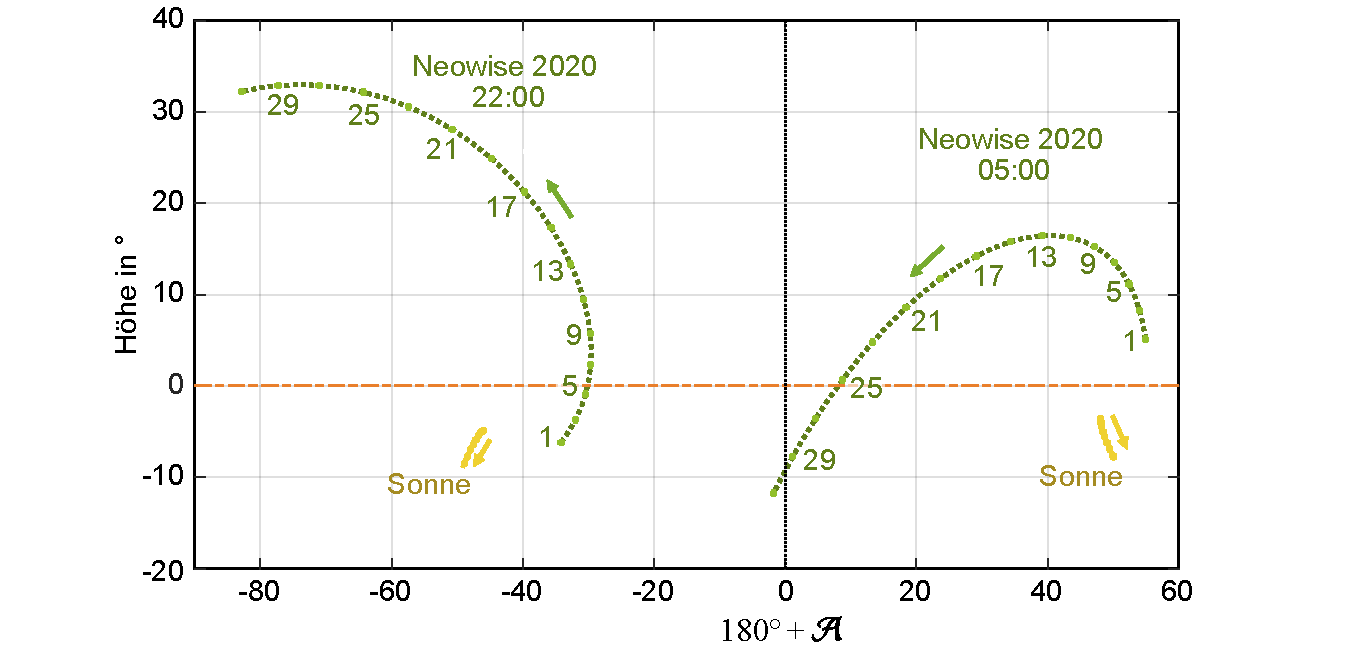
\includegraphics[width=\textwidth]{Neowise03.pdf}%
\caption{Berechnete Bahn des Kometen Neowise f�r den Monat Juli 2020.}%
\label{abb:hm_komet_neowise2}%
\end{figure}



\section{Berechnungen zu Sonnenfinsternissen}\label{kap:hm_sofis}\index{Sonnenfinsternis}\index{Mondfinsternis}

F�r Menschen ist eine totale Sonnenfinsternis (\figref{hm_Sofi2017})\footnote{Das Bild der totalen Sonnenfinsternis wurde mit einer Canon EOS700D und einem Celestron-Nexstar-5-Teleskop aufgenommen. Die Einzelbilder der partiellen Phasen wurden mit einer Canon 5D und einem 105-mm-Objektiv (M.~Kaschke, L.~Steger) fotografiert.} vermutlich mit eines der beeindruckendsten Ph�nomene, die man beobachten kann.
Die Kombination aus Seltenheit und K�rze einer solchen bogensekundengenau eintretenden Sonnenfinsternis (Englisch: \emph{Total Eclipse}), der abrupte Wechsel von Tag zu Nacht, das stundenlange Warten darauf und die oft tagelange Anreise in die h�ufig weit abgelegene Totalzone und nicht zuletzt das im Allgemeinen mit Jubel begr��te Wiedererscheinen der Sonne, all das macht das Erlebnis einer Sonnenfinsternis einzigartig und unvergesslich.
Wenn man bedenkt, dass bereits vor �ber 3000 Jahren Astronomen eine solche Sonnenfinsternis auf Minuten und wenige Kilometer genau vorhersagen konnten, kann man sich vorstellen, welche (nicht nur mentale) Macht diese Astronomen, die h�ufig auch die Hohepriester der herrschenden Dynastien waren, �ber die Menschen hatten.
Wir sind in der Lage, mit den in diesem Kapitel der Himmelsmechanik erarbeiteten Methoden und Kenntnissen diese Berechnungen selbst anzustellen.
Wir werden dabei nahezu das gesamte \anf{Handwerkszeug}, das wir in den vorausgehenden Kapiteln kennengelernt haben, anwenden k�nnen. 

\begin{figure}%
\centering\includegraphics[width=0.7\textwidth]{Sofi2017.jpg}%
\caption[Kompositaufnahme der Sonnenfinsternis 21.\,08.\,2017.]{Kompositaufnahme der Sonnenfinsternis 21.\,08.\,2017 am Snake River (Oregon/Idaho USA).} 
\label{abb:hm_Sofi2017}%Sofi2006
\end{figure}

\subsection{Mondbahn und Ekliptik -- Auftreten der Finsternisse}\label{kap:basics_sofis}

Wir beginnen zun�chst mit der Geometrie der Finsternisse.
Wiederum ist es bei der Betrachtung von Sonnen- und Mondfinsternissen vorteilhaft, in das geozentrische KOS zu wechseln.
Dazu werden wir das bereits in \kapitel{hm_naeherungsformeln_sonne} benutzte geozentrische Bild der \anf{scheinbaren} Bewegung der Sonne auf der Himmelssph�re (\figref{hm_wahre_sonne_geoz}) mit der Bahn des Erdmondes erg�nzen.
Dies ist in \figref{hm_Eclipse1} zu sehen.
Die Mondbahn hat eine Neigung von ca.$\:5\degree$ gegen�ber der Ekliptik und ihre Schnittpunkte mit der Ekliptik sind als \glslink{aufstknoten}{aufsteigender ($\ascnode$)}  \index{Knoten!aufsteigender} \bzw \glslink{abstknoten}{absteigender ($\descnode$) Knoten} \index{Knoten!absteigender} gekennzeichnet.

\begin{figure}%
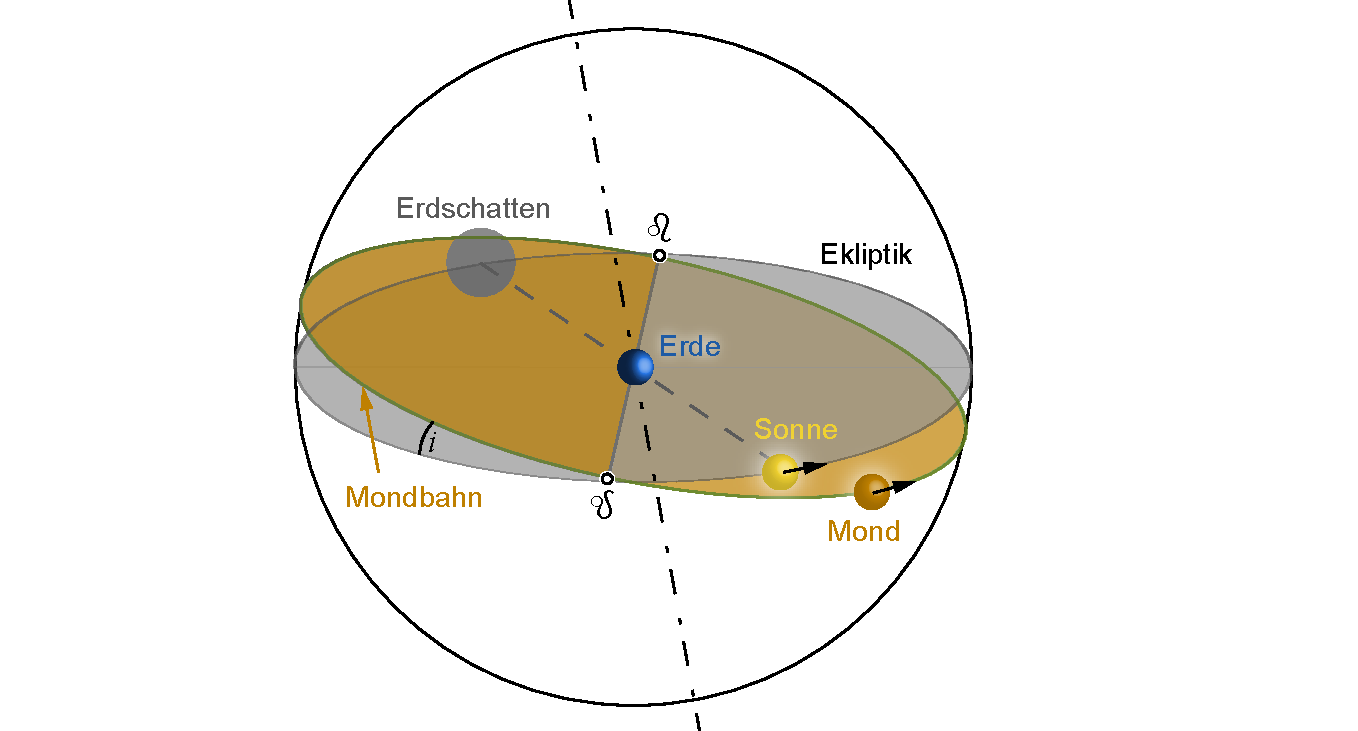
\includegraphics[width=\textwidth]{Eclipse1.pdf}%
\caption[Geozentrisches Bild der scheinbaren Bewegung von Sonne und Mond.]{Geozentrisches Bild der scheinbaren Bewegung von Sonne und Mond auf der Himmelssph�re.}%
\label{abb:hm_Eclipse1}%GeozentrGeometrie
\end{figure}

Da von der Erde aus betrachtet die scheinbaren Durchmesser\index{Durchmesser!scheinbarer} von Sonne und Mond einen etwa gleich gro�en Winkeldurchmesser von $0.5\degree$ haben, erscheinen beide Himmelsk�rper auch gleich gro� auf der Himmelssph�re.
Die Sonne \anf{durchl�uft} die Ekliptik einmal in einem tropischen Jahr.
Der Mond braucht f�r einen Bahnumlauf (z.\,B. von ${\ascnode}$ bis ${\ascnode}$) einen (siderischen) Monat.
Ebenfalls eingezeichnet ist der Schatten, den die Erdkugel auf die Himmelssph�re wirft.
Dieser hat in der Mondentfernung etwa einen Winkeldurchmesser von $1.4\degree$.
Man erkennt schon aus der Abbildung, dass Sonnen- und Mondfinsternisse nur in der N�he der Knoten stattfinden k�nnen, weil es sonst nicht zu einer Position der drei Himmelsk�rper kommt, in der sich die Schatten von Mond und Erde �berschneiden.
In \figref{hm_Eclipse2} haben wir solche m�glichen Konstellationen in der N�he des aufsteigenden Knotens $\ascnode$\glslink{aufstknoten}\ dargestellt. 
Wir betrachten zun�chst die Situationen bei Mondfinsternissen (\figref{hm_Eclipse2}a).
Offensichtlich gibt es eine Mondfinsternis nur bei Vollmond.
Die Sonne muss also (im Bild nicht dargestellt) in der N�he des absteigenden Knotens $\descnode$ der Mondbahn stehen: Der Erdschatten wandert durch den aufsteigenden Knoten $\ascnode$.
In der dargestellten Situation von Mond und Erdschatten\index{Erdschatten} kommt es dann zu einer partiellen Mondfinsternis.
Im Falle der Sonnenfinsternis stehen sowohl Sonne als auch Mond (und Mondschatten) in der N�he des Knotens.
Wir m�ssen uns daher von der Position des geozentrischen Beobachters l�sen und einen topozentrischen Beobachter auf der Erdkugel annehmen, da wegen der N�he des Mondes zur Erde dessen Parallaxe relativ gro� ist und nicht mehr vernachl�ssigt werden kann.
Folglich ist der Schattenbereich des Mondes, der von der Gesamtheit der Beobachter auf der Erdoberfl�che gesehen wird, gr��er als der Winkeldurchmesser des Mondes.
Mit anderen Worten: Die auf etwa $2\degree$ vergr��erten Schattenkreise enthalten alle Positionen der Mondoberfl�che, die von irgendeinem Punkt auf der Erdoberfl�che gesehen werden k�nnen.
Bei einer �berdeckung eines solchen Mondschattenkreises mit der Sonne, wie in der Situation in \figref{hm_Eclipse2}b dargestellt, kommt es zu einer (partiellen) Sonnenfinsternis.
Diese ist dann f�r bestimmte Punkte auf der Erdoberfl�che sichtbar.

\begin{figure}%
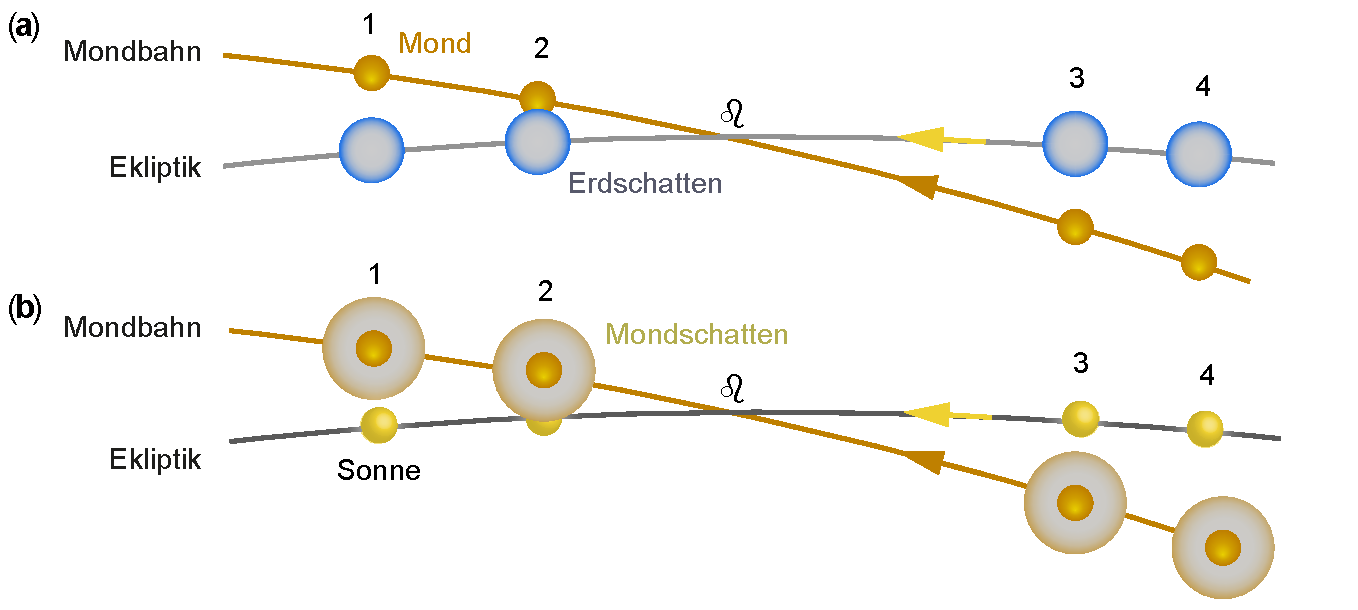
\includegraphics[width=\textwidth]{Eclipse2.pdf}%
\caption[Mond, Sonne und Schattenpositionen einer m�glichen Finsternis.]{Mond, Sonne und Schattenpositionen einer m�glichen Mondfinsternis. \fa Mondfinsternis (MF) und \fb Sonnenfinsternis (SF) am aufsteigenden Knoten der Mondbahn.}%
\label{abb:hm_Eclipse2}%AufsteigenederKnoten
\end{figure}

Mit diesem Verst�ndnis ist es nun m�glich, die Zeiten f�r eine m�gliche Sonnenfinsternis (oder Mondfinsternis) zu berechnen.
Wir m�ssen die Neumondzeitpunkte f�r Sonnenfinsternisse bzw. Vollmondzeitpunkte f�r Mondfinsternisse berechnen und die zu diesen Zeiten vorliegende ekliptikale geozentrische Breite des Neumondes $\beta_{\newmoon}$ bzw. Vollmondes $\beta_{\fullmoon}$ bestimmen.\footnote{Wir wollen uns im Folgenden auf die Sonnenfinsternis konzentrieren.
Alle Herleitungen gelten v�llig analog auch f�r die Mondfinsternis (siehe auch \probref{hm_MoFi}).}

Am einfachsten bestimmt man die Neumondzeiten, indem man die Funktion $\Delta \lambda (t)$ als Differenz der geozentrisch-ekliptikalen L�ngen von Sonne und Mond bildet,
\begin{equation}
  \Delta \lambda (t) = \lambda_\text{\astrosun} (t) - \lambda_\text{M} (t) \; ,
  \label{eq:hm_newmoon_determ}
\end{equation}
und die Nullstellen dieser Funktion ermittelt.\footnote{Nochmaliger Hinweis: Bei der Berechnung der Finsternis-Koordinaten ist darauf zu achten, dass man die Ephemeridenzeit ET benutzt und die Lichtlaufzeit von der Sonne zur Erde ber�cksichtigt.}
F�r die geozentrischen Koordinaten von Mond und Sonne haben wir in den \mscren entsprechende Routinen hinterlegt, die auch die relativ genauen analytischen Reihenentwicklungen f�r die Mond- und Sonnenbahn (siehe \kapitel{stoerungsrechnung}) verwenden.
Ein Berechnungsbeispiel f�r die Neumondzeiten �ber einen Zeitraum von 100 Jahren ist in \probref{hm_MoFi} zu finden.

\subsection{Schattengr��en und Orte einer totalen Sonnenfinsternis}
In \figref{hm_Eclipse3} haben wir die Schattenkegel\index{Schattenkegel}\index{Schattengr��e} eingezeichnet, die der Mond (hier auf die Erde) wirft.
Man erkennt einen \gls{ks}bereich\index{Kernschatten} (KS) und zwei Halbschattenbereiche\index{Halbschatten} (HS).
Je nach Abstand zwischen Erde und Mond kann es dann im KS-Bereich zur Ausbildung einer \glslink{tf}{totalen Finsternis}\index{Sonnenfinsternis!totale} (TF) oder einer \glslink{rf}{ringf�rmigen Finsternis}\index{Sonnenfinsternis!ringf�rmige} (RF) kommen.
Wir wollen den Durchmesser des Schattenkegels auf der Erdoberfl�che berechnen.
Aus \figref{hm_Eclipse4} k�nnen wir die geometrische Beziehung ableiten.
Wir starten mit
\begin{align*}
	q\sin\eta &= R_\text{M} ~~\text{und}\\
	(q + r_\text{\astrosun M})\,\sin\eta &= R_\text{\astrosun}\,.
\end{align*}
Daraus folgt sofort
\begin{align}
	\sin\eta &= \frac{R_\text{\astrosun} - R_\text{M}}{r_\text{\astrosun M}} ~~\text{und} ~~ 
	q = \frac{R_\text{M}\, r_\text{\astrosun M}}{R_\text{\astrosun} - R_\text{M}} \,.\label{eq:hm_sofi_basic01}
\end{align}

\begin{figure}%
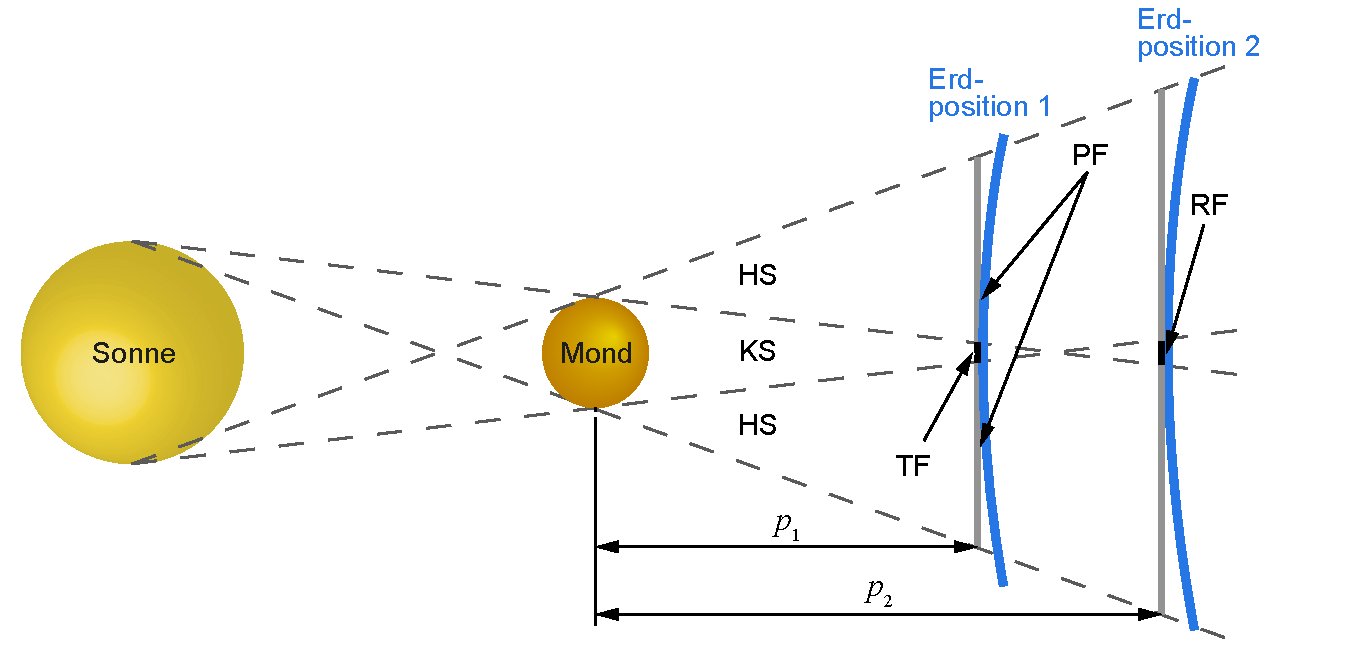
\includegraphics[width=\textwidth]{Eclipse3.pdf}%
\caption[Geometrie von Kern- und Halbschatten.]{Geometrie von Kern- und Halbschatten, sowie von totaler (TF), partieller (PF) und ringf�rmiger (RF) Sonnenfinsternis (Zur besseren Anschaulichkeit nicht ma�st�blich und auch nicht in den korrekten Proportionen gezeichnet!)}%
\label{abb:hm_Eclipse3}%Schatten- und Finsternisarten
\end{figure} 

\begin{figure}%
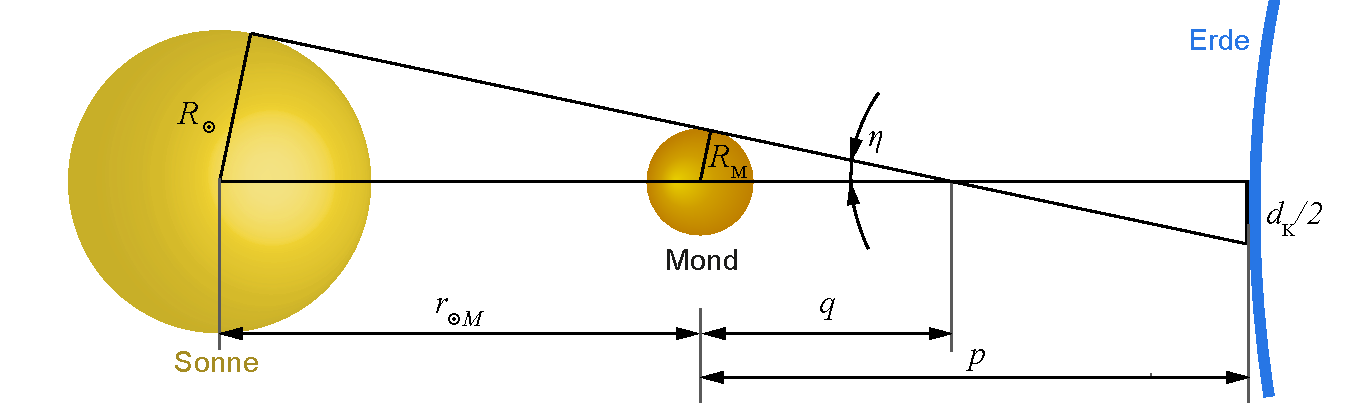
\includegraphics[width=\textwidth]{Eclipse4.pdf}%
\caption{Schattendurchmesser einer totalen Sonnenfinsternis.}%
\label{abb:hm_Eclipse4}%Schattendurchmesser
\end{figure}

Ferner k�nnen wir aus \figref{hm_Eclipse4} ablesen:
\begin{equation*}
\frac{d_\text{K}}{2} = (p-q)\,\tan\eta \,.
\end{equation*}
Mit der N�herung f�r kleine Winkel $\tan\eta\!\approx\!\sin\eta$ erh�lt man schlie�lich unter Nutzung von \eqref{eq:hm_sofi_basic01} f�r den Kernschattendurchmesser
\begin{align}
\frac{d_\text{K}}{2} &= \frac{p\,R_\text{\astrosun}}{r_\text{\astrosun M}} - \lk 1+\frac{p}{r_\text{\astrosun M}} \rk R_\text{M} ~ \nonumber\\
\rightarrow d_\text{K}(p) &= 2R_\text{\astrosun}\lk \frac{p}{r_\text{\astrosun M}} \rk - 2 R_\text{M} \lk 1+\frac{p}{r_\text{\astrosun M}}\rk \,. \label{eq:hm_schattenkegel1}
\end{align}
Setzt man die Werte $2R_\text{\astrosun}\!=\! 218.4 R_\text{\earth}$ und $2R_\text{M}\!=\! 0.545 R_\text{\earth}$ ein und nimmt in guter N�herung $r_\text{\astrosun M}\!\approx\! 1\:\text{AE} - 380000\:\text{km}\pm 25000\:\text{km}$ an, dann findet man f�r den Kernschattendurchmesser Werte zwischen $250$ und $350\:$km.
Das hei�t, dass nur ein kleiner Teil der Erdoberfl�che vom Kernschatten getroffen wird, was die oft langen Reisen zu den Finsternisorten erkl�rt.
Entsprechend gilt f�r den Halbschattendurchmesser
\begin{align}
D_\text{H}(p) &= 2R_\text{\astrosun}\lk \frac{p}{r_\text{\astrosun M}} \rk + 2 R_\text{M} \lk 1+\frac{p}{r_\text{\astrosun M}}\rk \,. \label{eq:hm_schattenkegel2}
\end{align}

\begin{figure}%
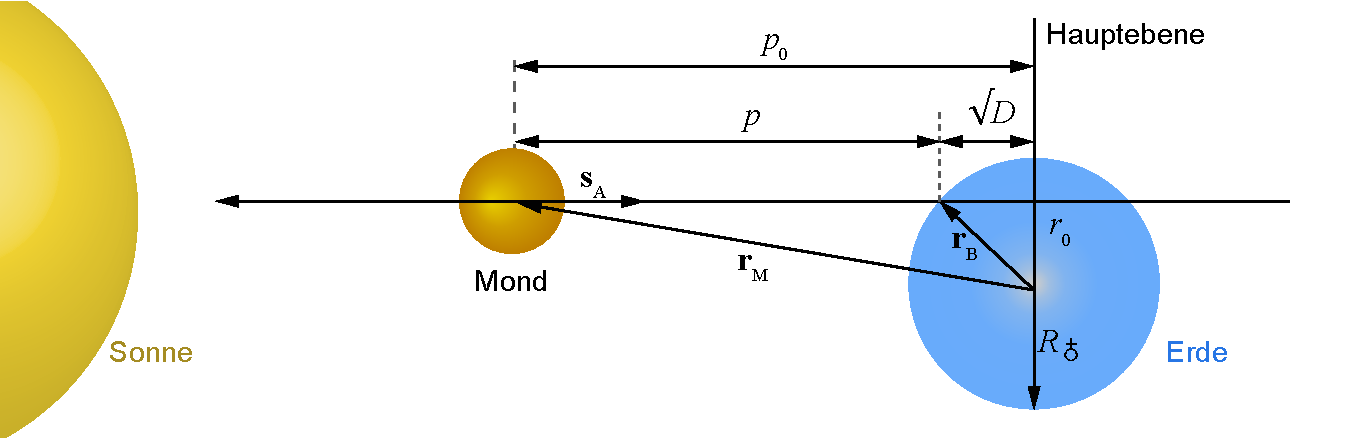
\includegraphics[width=\textwidth]{Eclipse5.pdf}%
\caption[Auftreffpunkt der Kernschattenachse auf der Erdoberfl�che.]{Berechnung des Auftreffpunktes der Kernschattenachse auf der Erdoberfl�che.}%
\label{abb:hm_Eclipse5}%Schnittpunkt Schattenachse
\end{figure}
Den Ort des Auftreffens der Achse des KS-Kegels ermitteln wir mit Hilfe von \figref{hm_Eclipse5}.
Die Achse $\vec{s}_\text{A}$ wird durch die Richtung von der Sonnenmitte zur Mondmitte definiert und kann andererseits als
\begin{equation}
\vec{s}_\text{A} = \frac{\vec{r}_\text{B} - \vec{r}_\text{M}}{\abs{\vec{r}_\text{B} - \vec{r}_\text{M}}} ~\label{eq:hm_achse_ks_kegel}
\end{equation}
beschrieben werden.
Hierin sind $\vec{r}_\text{M}$ der geozentrische Ortsvektor des Mondes und $\vec{r}_\text{B}$ der Vektor des Auftreffpunktes der Schattenachse auf der Erdoberfl�che, also dort, wo sich ein Beobachter einer TF idealerweise befinden sollte.
Aus \figref{hm_Eclipse5} lesen wir ferner ab, dass
\begin{align}
	\vec{r}_\text{B} &= \vec{r}_\text{M} + p\,\vec{s}_\text{A} = \lk \begin{matrix} x_\text{M} + p \,s_{\text{A},x} \\ y_\text{M} + p \,s_{\text{A},y} \\z_\text{M} + p \,s_{\text{A},z}\end{matrix}\rk\, = \,\lk \begin{matrix} x_\text{B} \\ y_\text{B} \\ z_\text{B} \end{matrix} \rk \,, \label{eq:hm_auftreffvek}\\
	\vec{r}_\text{B}^2 &= x_\text{B}^2 + y_\text{B}^2 + z_\text{B}^2 = R_\text{\earth}^2 \,. \label{eq:hm_auftreffvek2}
\end{align}
In \eqref{eq:hm_auftreffvek2} haben wir zun�chst noch die Kugelgestalt der Erde angenommen.
Setzt man nun \eqref{eq:hm_auftreffvek} in \eqref{eq:hm_auftreffvek2} ein, ergibt sich
\begin{equation*}
p^2 + 2p \,\vec{r}_\text{M}\,\vec{s}_\text{A} + (r_\text{M}^2 - R_\text{\earth}^2) = 0
\end{equation*}
mit den L�sungen
\begin{equation}
p = p_0 \pm \sqrt{D} \,,\label{eq:hm_lsg_p}
\end{equation}
worin $p_0$ und $D$ durch
\begin{align*}
	p_0 &= - \lk x_\text{M} e_x + y_\text{M} e_y + z_\text{M} e_z\rk ~~\text{\bzw} ~~	D = p_0^2 + R_\text{\earth}^2 - r_\text{M}^2 \,
\end{align*}
gegeben sind. Physikalisch sinnvoll ist nur die L�sung mit dem negativen Vorzeichen, da diese einen Punkt auf der Tagseite der Erde beschreibt.
Die L�sung $p = p_0 + \sqrt{D}$ beschreibt einen Punkt auf der Nachtseite der Erde.
Falls $D\!<\!0$, l�uft die Schattenachse an der Erde vorbei und es kommt zu keiner Finsternis.
Damit haben wir den \anf{Zentralort} der totalen Finsternis auf der Erdoberfl�che bestimmt:
\begin{equation}
\vec{r}_\text{B} = \vec{r}_\text{M} + (p_0 - \sqrt{D}) \,\vec{s}_\text{A} \,. \label{eq:hm_zentralort_tot_finsternis}
\end{equation} 
Damit eine totale Sonnenfinsternis auftreten kann, muss gem�� \figref{hm_Eclipse5} noch gelten, dass
\begin{equation*}
r_\text{M}^2 - p_0^2 < R_\text{\earth}^2 \,.
\end{equation*}
Bisher haben wir die Erde als perfekte Kugel betrachtet.
Jetzt m�ssen wir deren Abplattung ber�cksichtigen.
Die Erde kann als Rotationsellipsoid mit einem um $(1-f) = 0.996647$ gestauchten Polarradius gegen�ber dem mittleren Radius $R_\text{\earth}$ angenommen werden.
Die bisherigen Rechnungen kann man gl�cklicherweise einfach weiter verwenden, indem man in \eqref{eq:hm_auftreffvek2} die $z$-Koordinate der Beobachterkoordinaten um den Betrag der Abplattung $(1-f)$ staucht. \eqref{eq:hm_auftreffvek2} lautet dann
\begin{align}
		\vec{r}_\text{B}^2 &= x_\text{B}^2 + y_\text{B}^2 + z_\text{B}^2 \, (1-f)^2 = R_\text{\earth}^2 \,. \label{eq:hm_auftreffvek3}
\end{align}
Alle anderen Berechnungsschritte bleiben wie oben dargestellt.

\subsection{Ber�cksichtigung der Abplattung der Erde}
Wir m�ssen zur Ortsbestimmung der Finsternis noch die Rotation der Erde ber�cksichtigen.
Ohne Abplattung der Erde w�re das relativ einfach, weil wir aus den geozentrischen Koordinaten des Mondes �ber die Deklination direkt die Breite des Beobachtungspunktes erhielten und aus der Rektaszension des Mondes �ber die Sternzeit auch die geographische L�nge berechnen k�nnten.
Durch die Abplattung der Erde ist aber die geographische Breite nicht gleich der geozentrischen Breite (die wiederum der Deklination entspricht).
F�r die Umrechnung \glslink{geozentrkoord} von geozentrischen $(\varphi_\text{B}',\,\lambda'_\text{B})$ in geographische\index{Koordinaten!geographische} Koordinaten $(\varphi_\text{B},\,\lambda_\text{B})$ eines Beobachtungspunktes auf der Erde besteht in guter N�herung der Zusammenhang \cite{Montenbruck1999}:
\begin{align}
\varphi &= \varphi' + 0.1924\degree\,\sin(2\varphi')\; , \qquad ~~\lambda = \lambda'\,. \label{eq:hm_umrechnung_geogr_geozent_Koord}
\end{align}
Die geographische L�nge kann �ber die bekannte Beziehung \eqref{eq:hm_LMST} mittels der Sternzeit $\theta(t)$ aus der Rektaszension berechnet werden (siehe \kapitel{hm_raum_und_zeit}):
\begin{equation}
\alpha = \theta_0(t) + \lambda\,a\,e \; .\label{eq:hm_geogr_laenge_rektaszension}
\end{equation}
Damit kann der Ortsvektor des Auftreffpunktes der Schattenachse auf der Erdoberfl�che geschrieben werden als
\begin{align}
\lk \begin{matrix} x_\text{B} \\ y_\text{B} \\ z_\text{B} \end{matrix}\rk &= \lk \begin{matrix} r_\text{B}\cos\varphi' \cos\lambda \\ r_\text{B}\cos\varphi' \sin\lambda \\ r_\text{B}\sin\varphi' \end{matrix}\rk = \mathbb{R}_z\lk\theta(t)\rk\,\lk \begin{matrix} r_\text{B}\cos\delta \cos\alpha \\ r_\text{B}\cos\delta \sin\alpha \\ r_\text{B}\sin\delta \end{matrix}\rk \,. \label{eq:hm_schattenachse_auf_erde}
\end{align}
Zur Erinnerung $x_\text{B}, y_\text{B}, z_\text{B}, r_\text{B}$ sind bekannt \bzw berechnet, bestimmt werden aus \eqref{eq:hm_schattenachse_auf_erde} $\lambda, \varphi'$.
Ebenfalls sei nochmals der Hinweis gegeben, dass die Koordinatenberechnung $(\alpha,\,\delta)$ immer mit der ET zu erfolgen hat.
F�r die Berechnung der Sternzeit brauchen wir aber nach Gleichung \eqref{eq:hm_UT_3} die UT.
Zwischen beiden Zeiten besteht ein Unterschied $\Delta T$.
Man muss diesen also f�r den Zeitraum der Finsternis kennen oder zumindest �ber N�herungs-Polynome \cite{Espenak2014} absch�tzen k�nnen.
Mit \eqref{eq:hm_schattenachse_auf_erde} k�nnen wir nun den geographischen Ort $(\varphi(\varphi'=\delta),\,\lambda(\alpha))$ zur Zeit des Auftretens des Schattenkegels der Sonnenfinsternis berechnen.
Die Linie entlang aller geographischen Orte, die so zu den verschiedenen Zeitpunkten der maximalen Finsternis berechnet werden, wird Zentrallinie genannt. 

\subsection{Finsternisdauer}\index{Sonnenfinsternis!Dauer}
Mit den Beziehungen \eqref{eq:hm_lsg_p} und \eqref{eq:hm_zentralort_tot_finsternis} lassen sich zu dem mittels \eqref{eq:hm_newmoon_determ} ermittelten Finsterniszeitpunkt $t_0$ die kartesischen Koordinaten des Schattenkegels zu
\begin{align}
\vec{r}_\text{B0}(t_0) &= \lk \begin{matrix} x_\text{B0}(t_0) \\ y_\text{B0}(t_0) \\ z_\text{B0}(t_0)\end{matrix} \rk
\label{eq:hm_schatten_kartes_1}
\end{align}
und zu einem etwas sp�teren Zeitpunkt $t_1\!=\!t_0+\Delta t$ zu
\begin{align}
\vec{r}_\text{B1}(t_1) &= \lk \begin{matrix} x_\text{B1}(t_1) \\ y_\text{B1}(t_1) \\ z_\text{B1}(t_1)\end{matrix} \rk \label{eq:hm_schatten_kartes_2}
\end{align}
berechnen.
$(\vec{r}_\text{B1} - \vec{r}_\text{B0})/\Delta t$ ist dann ein Ma� f�r die Geschwindigkeit, mit der sich der Kernschatten fortbewegt.
Um aber die Bewegung des Schattens relativ zur Erdoberfl�che zu berechnen, muss man noch die Rotation der Erde ber�cksichtigen, denn in der Zeit $\Delta t$ dreht sich die Erde um einen Winkel
\begin{equation}
\xi = \frac{2\pi\!\Delta t}{d_\diamond} \,. \label{eq:hm_winkeldrehung_erde}
\end{equation}
Hierin ist $d_\diamond$ die Dauer eines Sterntages. In der Zeitspanne $\Delta t$ haben sich also die �quatorialen Koordinaten des Punktes $\vec{r}_\text{B1}(t_0+\Delta t)$ durch Drehung so ver�ndert, dass dieser Punkt zur Zeit $t_0$ die Koordinate
\begin{equation}
\vec{r}'_\text{B1} (t_0) = \mathbb{R}_z(\xi)\,\vec{r}_\text{B1}(t_1) ~ \label{eq:hm_koord_nach_winkeldrehung}
\end{equation}
hat.
Der Kernschatten legt folglich im Zeitraum $\Delta t$ bezogen auf das \emph{earth-fixed} KOS (siehe \kapitel{hm_koordinatensysteme}) den Weg $\Delta\vec{r}\!=\!\vec{r}'_\text{B1}-\vec{r}_\text{B0}$ zur�ck.
Da $\Delta t$ eine kurze Zeit ist, kann man die Rotationsmatrix $\mathbb{R}_z(\xi)$ f�r kleine Winkel $\xi$ vereinfachen und n�herungsweise schreiben:

\begin{equation*}
\Delta\vec{r} = \lk \begin{matrix} \Delta x \\ \Delta y \\ \Delta z \end{matrix}\rk  = \lk \begin{matrix} x'_\text{B1} \\ y'_\text{B1} \\ z'_\text{B1} \end{matrix}\rk - \lk \begin{matrix} x_\text{B0}\\ y_\text{B0} \\ z_\text{B0} \end{matrix}\rk = \lk \begin{matrix} x_\text{B1} + \xi y_\text{B1} - x_\text{B0} \\ y_\text{B1} - \xi x_\text{B1} - y_\text{B0} \\ z_\text{B1} - z_\text{B0} \end{matrix}\rk\,\,.
\end{equation*}


Unter Benutzung von \figref{hm_Eclipse5} zerlegt man $\Delta\vec{r}$ in einen Anteil parallel zu $\vec{e}$ und einen Anteil senkrecht zu $\vec{e}$:
\begin{align*}
	\Delta r_\parallel &= \Delta\vec{r}\cdot\vec{e} = \Delta x\,e_x + \Delta y\, e_y + \Delta z\, e_z ~~\text{und} \\
	\Delta r_\perp &= \sqrt{\Delta r^2 - \Delta r_\parallel^2} \,.
\end{align*}
Die tats�chliche, effektive Geschwindigkeit, mit der sich der Kernschatten senkrecht zur Einfallrichtung des Schattenkegels weiterbewegt, ist $v_\perp\!=\!\Delta r_\perp / \Delta t$.
Die Dauer der totalen Finsternis an einem Punkt ist dann gegeben durch
\begin{equation}
t_z = \frac{\abs{d}}{v_\perp}\,, \label{eq:hm_dauer_kernschatten}
\end{equation}
worin $d$ der nach \eqref{eq:hm_schattenkegel1} berechnete Durchmesser des Kernschattens zur jeweiligen Zeit ist.

Wir haben damit alle Berechnungsformeln, um den Zeitpunkt, den geographischen Ort (inkl.\ Breite der Totalit�tszone) und die Dauer der Totalit�t zu berechnen.

\subsection{Zusammenfassende Darstellung des Algorithmus in \matlab}
Wir gehen im Folgenden noch einmal zusammenfassend die Einzelschritte zur Berechnung der Daten f�r eine totale Sonnenfinsternis an, wie diese auch in den \mscren \mlhmref{Sonnenfinsternis01.m}, \mlhmref{Sonnenfinsternis02.m} und \mlhmref{Sonnenfinsternis03.m} hinterlegt sind.
Wir folgen hierbei der exzellenten Darstellung des Themas in \cite{Montenbruck1999}, haben diese aber auf die Berechnungen in \matlab{} angepasst. 

\begin{enumerate}[1.]
  \item Mit Hilfe der \mscre \mlhmiref{SonneExakt.m} und \mlhmiref{MondExakt.m}  berechnen wir die geozentrisch-ekliptikalen Koordinaten von Sonne und Mond und untersuchen die Funktion $\Delta \lambda (t)\!=\!\lambda_\text{\astrosun} (t)\!-\!\lambda_\text{M} (t)$ �ber einen bestimmten Zeitraum hinweg auf Nullstellen.
          Dabei ist als Zeit ET zu nehmen.
          F�r die Sonne m�ssen wir wegen der Lichtlaufzeit $\tau_\text{\,L}\!=\!8.32 \:\text{min}$ die Zeiten entsprechend zur�ckversetzt berechnen.
	\item Gibt es eine Nullstelle $t_0$, so wird an dieser die geozentrisch-ekliptikale Breite des Neumondes $\beta_\text{\newmoon}$ bestimmt.
          Ist $\left| \beta_\text{\newmoon} \right| < 52'$ dann ist eine totale Sonnenfinsternis sicher, bei $\left| \beta_\text{\newmoon} \right| > 1\degree\:35'$ ist keine Finsternis (weder total noch partiell) m�glich.
          Kommt es zu einer Finsternis, dann nennen wir die Neumondzeit $t_0 = t_\text{F}$.
	\item Von diesem Zeitpunkt aus betrachten wir einen Zeitraum von $t_\text{F} - 6 \text{h}$ bis $t_\text{F} + 6 \text{h}$ und berechnen in Intervallen von ein bis zwei Minuten die Koordinaten des Schnittpunktes der Schattenachse mit der Erde zum jeweiligen Zeitpunkt.
          Wir ber�cksichtigen dabei die Abplattung der Erde, indem wir die $z$-Koordinate entsprechend \eqref{eq:hm_auftreffvek3} korrigieren.
          Wiederum m�ssen wir bei der Berechnung der Schattenachse die Lichtlaufzeit $\tau_\text{ L}$ ber�cksichtigen.
          Wir erhalten so die geographischen Koordinaten\index{Koordinaten!geographische} der Zentrallinie der Sonnenfinsternis.
	\item �ber die Geschwindigkeit des Kernschattens und \eqref{eq:hm_dauer_kernschatten} erhalten wir die Dauer der Sonnenfinsternis f�r den jeweiligen Punkt auf der Zentrallinie.
	\item Wir k�nnen noch f�r beliebige Orte und Zeiten (entlang oder abseits der Zentrallinie) weitere Daten �ber den Ablauf der Sonnenfinsternis wie die Kontaktzeiten oder den Grad der Verfinsterung berechnen.
          Dabei gehen wir folgenderma�en vor:
	\begin{enumerate} [(a)]
		\item Wir w�hlen eine Zeit $t$ um die Finsterniszeit $t_\text{F}$ und geographische Koordinaten $(\varphi,\,\lambda)$.
		\item Aus den geozentrisch-�quatorialen Koordinaten von Sonne und Mond bestimmen wir die Richtung der Schattenachse und die senkrecht dazu liegende Hauptebene durch den Erdmittelpunkt (\figref{hm_Eclipse5}).
		\item Wir berechnen dann �ffnungswinkel $\eta$ und Radien der Schattenkegel auf der Hauptebene nach \eqref{eq:hm_schattenkegel1} \bzw \eqref{eq:hm_schattenkegel2}.
                  Eleganter weise legen wir dazu ein weiteres kartesisches $u$-$v$-$w$-\,KOS fest, dessen $w$-Achse die Richtung der Schattenachse hat und dessen $u$-Achse senkrecht auf der Schattenachse steht und in der �quatorebene der Erde liegt.
		\item In diesem KOS berechnen wir auch die Koordinaten des Mondes ($u_\text{M}$, $v_\text{M}$, $w_\text{M}$).
		\item Mit den in geozentrische Koordinaten\glslink{geozentrkoord}\ umgerechneten geographischen Koordinaten\index{Koordinaten!geographische} des Beobachtungsortes berechnen wir dessen Projektionskoordinaten auf die Hauptebene ($u_\text{B}$, $v_\text{B}$, $w_\text{B}$).
		\item Mit diesen Werten k�nnen wir den Abstand $\Delta A_\text{BS}\!=\!A_\text{BS}\!-\! d$ des Beobachters vom Rand des Schattenkegels bestimmen.
                  Ist $\Delta A_\text{BS}\!=\! 0$, dann liegt der Beobachter genau auf dem Rand des Schattenkegels (Halbschatten oder Kernschatten).
                  Bei $\Delta A_\text{BS}\!=\! -d$ liegt er genau auf der Zentrallinie.
		\item Damit k�nnen wir die sogenannten Kontaktzeiten -- das sind die \anf{Ber�hrungen} des Beobachterortes durch die Schattenkreise -- bestimmen.
                  Diese werden durch die Nullstellen der Funktion $\Delta A_\text{BS}$ ermittelt, und zwar zun�chst f�r den Halbschatten-Kreis (1.\ und 3.\ Kontaktzeit) und dann f�r den Kernschatten (2.\ und 3.\ Kontaktzeit).
		\item Ebenso k�nnen wir auf diese Weise numerisch das Minimum von $\Delta A_\text{BS}$ ermitteln.
                  Das ergibt dann den Zeitpunkt und Grad der maximalen Verfinsterung.
	\end{enumerate}
\end{enumerate}

Damit haben wir die Charakteristika einer Sonnenfinsternis ziemlich umfassend berechnet.
In den Tabellen \ref{tab:hm_Zentrallinie2017} und \ref{tab:hm_Beobachtung1999_2017} sind die mit den \mscren \mlhmref{Sonnenfinsternis01.m}--\mlhmref{Sonnenfinsternis03.m} berechneten Werte f�r die beobachteten Sonnenfinsternisse in den Jahren 1999, 2006 und 2017 gelistet.
An die in den Programmen verwendeten Routinen f�r die Positionsberechnung von Sonne und Mond werden extrem hohe Anforderungen gestellt.%
\footnote{Um die Zeiten der Verfinsterung auf eine Sekunde genau berechnen zu k�nnen, braucht man Genauigkeiten in der Ephemeridenrechnung von etwa einer Bogensekunde.
Die \mscre \mlhmiref{SonneExakt.m} und \mlhmiref{MondExakt.m} wurden auf Basis von Daten aus \cite{Montenbruck1999, Meeus1998} geschrieben und liefern damit Genauigkeiten von besser als 5 Bogensekunden �ber einen Zeitraum von mehreren Jahrzehnten.
Die in den Tabellen \ref{tab:hm_Zentrallinie2017} und \ref{tab:hm_Beobachtung1999_2017} aufgef�hrten Werte einige Sekunden von den in astronomischen Almanachen angegebenen Werten abweichen, da die zu Grunde liegenden Algorithmen verschieden sein k�nnen.}
\figref{hm_Eclipse6} zeigt den Verlauf dieser und der kommenden mit �ber 4 Minuten totaler Finsternis relativ langen Sonnenfinsternis von 2024.
Man sieht, dass Orte gibt, die im Abstand von 7 Jahren zweimal in den Genuss einer totalen Sonnenfinsternis kommen. 

\begin{table}
\caption{Berechnung der Zentrallinie der Sonnenfinsternis von 2006.}
\centering\begin{tabular}{R{1cm}R{1cm}R{1.5cm}R{1.5cm}R{1.5cm}L{1.5cm}}
\hline\noalign{\smallskip}
Datum	& UT & $\varphi\,[\degree ']$ & $\lambda \,[\degree ']$ & Dauer [min:s] & Phase \\
\noalign{\smallskip}\svhline\noalign{\smallskip}
29.\,03.\,2006 & 08:00 &--- &	--- &	---& partiell \\
29.\,03.\,2006 & 08:10 &--- &	--- &	---& partiell \\
29.\,03.\,2006 & 08:20 &--- &	--- &	---& partiell \\
29.\,03.\,2006 & 08:30 &--- &	--- &	---& partiell \\
29.\,03.\,2006 & 08:40 & - 04 05 &	 - 25 33 &	 2:28 & total \\
29.\,03.\,2006 & 08:50 & - 00 42 &	 - 11 50 &	 2:56 & total \\
29.\,03.\,2006 & 09:00 & + 02 24 &	 - 05 42 &	 3:16 & total \\
29.\,03.\,2006 & 09:10 & + 05 24 &	 - 01 08 &	 3:30 & total \\
29.\,03.\,2006 & 09:20 & + 08 21 &	 + 02 34 &	 3:43 & total \\
29.\,03.\,2006 & 09:30 & + 11 15 &	 + 05 46 &	 3:52 & total \\
29.\,03.\,2006 & 09:40 & + 14 08 &	 + 08 37 &	 4:00 & total \\
29.\,03.\,2006 & 09:50 & + 17 00 &	 + 11 17 &	 4:05 & total \\
29.\,03.\,2006 & 10:00 & + 19 54 &	 + 13 52 &	 4:09 & total \\
29.\,03.\,2006 & 10:10 & + 22 38 &	 + 16 26 &	 4:11 & total \\
29.\,03.\,2006 & 10:20 & + 25 42 &	 + 19 05 &	 4:10 & total \\
29.\,03.\,2006 & 10:30 & + 28 40 &	 + 21 55 &	 4:07 & total \\
29.\,03.\,2006 & 10:40 & + 31 39 &	 + 25 02 &	 4:02 & total \\
29.\,03.\,2006 & 10:50 & + 34 42 &	 + 28 36 &	 3:46 & total \\
29.\,03.\,2006 & 11:00 & + 37 47 &	 + 32 47 &	 3:45 & total \\
29.\,03.\,2006 & 11:10 & + 40 57 &	 + 37 54 &	 3:34 & total \\
29.\,03.\,2006 & 11:20 & + 44 10 &	 + 44 30 &	 3:19 & total \\
29.\,03.\,2006 & 11:30 & + 47 25 &	 + 53 38 &	 3:00 & total \\
29.\,03.\,2006 & 11:40 & + 50 32 &	 + 68 21 &	 2:34 & total \\
29.\,03.\,2006 & 11:50 & --- 	 &	 ---  		&	--- & partiell \\
29.\,03.\,2006 & 12:00 & ---  	 &	 ---  		&	 --- & partiell \\
\noalign{\smallskip}\hline\noalign{\smallskip}
\end{tabular}
\label{tab:hm_Zentrallinie2017}
\end{table}

\begin{figure}%
\includegraphics[width=\textwidth]{SolarEclipseLines.pdf}%
\caption[Pfad der Sonnenfinsternisse von 1999, 2006, 2017 und 2024.]{Pfad der Sonnenfinsternisse von 1999, 2006, 2017 und 2024. Die blauen Pfeile markieren die jeweiligen Beobachtungsorte, an denen von den Autoren Aufnahmen und Messungen gemacht wurden, die in den �bungen Eingang gefunden haben.}%
\label{abb:hm_Eclipse6}%
\end{figure}

\begin{table}
\caption[Beobachtungsdaten am Beobachtungsort der Sonnenfinsternis 1999.]{Beobachtungsdaten am Beobachtungsort der Sonnenfinsternis 1999 (11.08.1999: Oberkochen (D): $\varphi\!=\!48.1\degree$, $\lambda\!=\!10.9\degree$) und 2017 (21.08.2017: Snake River Idaho (USA): $\varphi\!=\!44.3\degree$, $\lambda\!=\!-117.1\degree$).}
\centering
\begin{tabular}{L{1.5cm}L{2cm}L{1.5cm}L{2cm}}
\hline\noalign{\smallskip}
Datum	& Zeitpunkt (UT) & Phase & Bemerkung \\
\noalign{\smallskip}\svhline\noalign{\smallskip}
11.\,08.\,1999 & 09:15:39 & partiell & 	1.\ Kontakt \\
11.\,08.\,1999 & 10:36:38 & total & 	2.\ Kontakt \\
11.\,08.\,1999 & 10:37:26 & total & 	Maximum \\
11.\,08.\,1999 & 10:38:18 & total & 	3.\ Kontakt \\
11.\,08.\,1999 & 12:00:42 & partiell & 	4.\ Kontakt \\
\hline\noalign{\smallskip}
Datum	& Zeitpunkt (UT) & Phase & Bemerkung \\
\noalign{\smallskip}\svhline\noalign{\smallskip}
21.\,08.\,2017 & 16:10:19 & partiell & 	1.\ Kontakt \\
21.\,08.\,2017 & 17:25:13 & total & 	2.\ Kontakt \\
21.\,08.\,2017 & 17:26:14 & total & 	Maximum \\
21.\,08.\,2017 & 17:27:24 & total & 	3.\ Kontakt \\
21.\,08.\,2017 & 18:48:28 & partiell & 	4.\ Kontakt \\
\noalign{\smallskip}\hline\noalign{\smallskip}
\end{tabular}
\label{tab:hm_Beobachtung1999_2017}
\end{table}

%%%%%%%%%%%%%%%%%%%%%%%%%%%%%%%%%%%%%%%%%%%%%%%%%%%%%%%%%%%%%%%%%%%%%%%%%%



\section{Gezeiten}\index{Gezeiten}\label{kap:hm_gezeiten}

Wir sind den Begriffen Gezeiten und Gezeitenkr�fte bereits in Kapitel 1 (Band I) begegnet.
Obwohl im allgemeinen Sprachgebrauch der Begriff Gezeiten fast ausschlie�lich mit dem Ph�nomen von Ebbe und Flut der Ozeane verkn�pft wird, sind Gezeitenkr�fte viel fundamentaler und treten �berall dort auf, wo die r�umliche Ausdehnung der K�rper in einem gravitativen System nicht mehr zu vernachl�ssigen ist.
Im Umkehrschluss treten Gezeitenkr�fte bei idealisierten Systemen von Punktmassen nicht auf.
Wir werden deshalb jetzt das Massepunktmodell verlassen und die Ausdehnung und geometrische Form von Himmelsk�rpern ber�cksichtigen.
%
\subsection{�bergang von Punktmassen zu ausgedehnten K�rpern} \label{kap:hm_gezeite_Recap}

Im Band I hatten wir uns mit den theoretischen Grundlagen der Gezeiten besch�ftigt.
Wir hatten gelernt, dass es immer dann zu Gezeitenkr�ften kommt, wenn die Inhomogenit�t des Gravitationsfeldes zu unterschiedlichen Kraftwirkungen auf einen K�rper f�hrt.
Gezeitenkr�fte haben %im Gegensatz zur Newtonschen Gravitationskraft mit ihrer $1/r^2$-Abh�ngigkeit 
eine $1/r^3$ Abh�ngigkeit und treten nur dann f�r einen ausgedehnten K�rper der Masse $m$ auf, wenn sich dieser in einem inhomogenen Gravitationsfeld befindet/bewegt.
In einem homogenen Gravitationsfeld w�rde der K�rper ohne Einfluss weiterer Kr�fte an jedem Ort dieselbe Beschleunigung sp�ren. Reale Gravitationsfelder sind aber niemals homogen.
\footnote{Da die Quelle des Gravitationsfeldes ausschlie�lich positive Massen sind, kann es anders als in der Elektrodynamik \bzw Elektrostatik keine homogenen Felder geben. Da ein Massepunkt per Definition keine Ausdehnung hat, gibt es f�r diesen auch keine Gezeitenkr�fte.}
Wir haben das anhand einer Testanordnung aus $36$ gleichen (kleinen) Massen demonstriert, die sich zum Zeitpunkt $t_0$ im Schwerefeld einer gro�en Masse $M$ befinden und anf�nglich einen kreisf�rmigen Ring bilden.
Die Gezeitenkr�fte, die auf diese Testanordnung wirken, ergeben sich als Differenz zur mittleren Schwerkraft, die auf die Masse im Zentrum des Rings wirkt, und bewirken mit der Zeit eine ellipsen- \bzw birnenf�rmige Verformung des Rings (\figref{hm_gezeiten01}).\\

Man kann Gezeitenwirkungen an einer Vielzahl von Ph�nomenen und Systemen in der Himmelsmechanik beobachten.
Als Beispiele seien genannt %\cite{Gomer2020, Hebelacker1998}
\begin{itemize}
    \item die Pr�zession der Erdachse (\vgl Kap. 1.5.6 (Band I)),
    \item das Auseinanderbrechen von Kometen (\vgl Beispiel Shoemaker-Levy, in \kap{kometen} behandelt),
    \item die Beeinflussung planetarer Ringe,
    \item der Vulkanismus auf Kleink�rpern, die sich um massive Zentralk�rper bewegen und
    \item die R�ckwirkung von (gro�en) Exoplaneten auf deren Sonnen.
\end{itemize}

\begin{figure}[H]
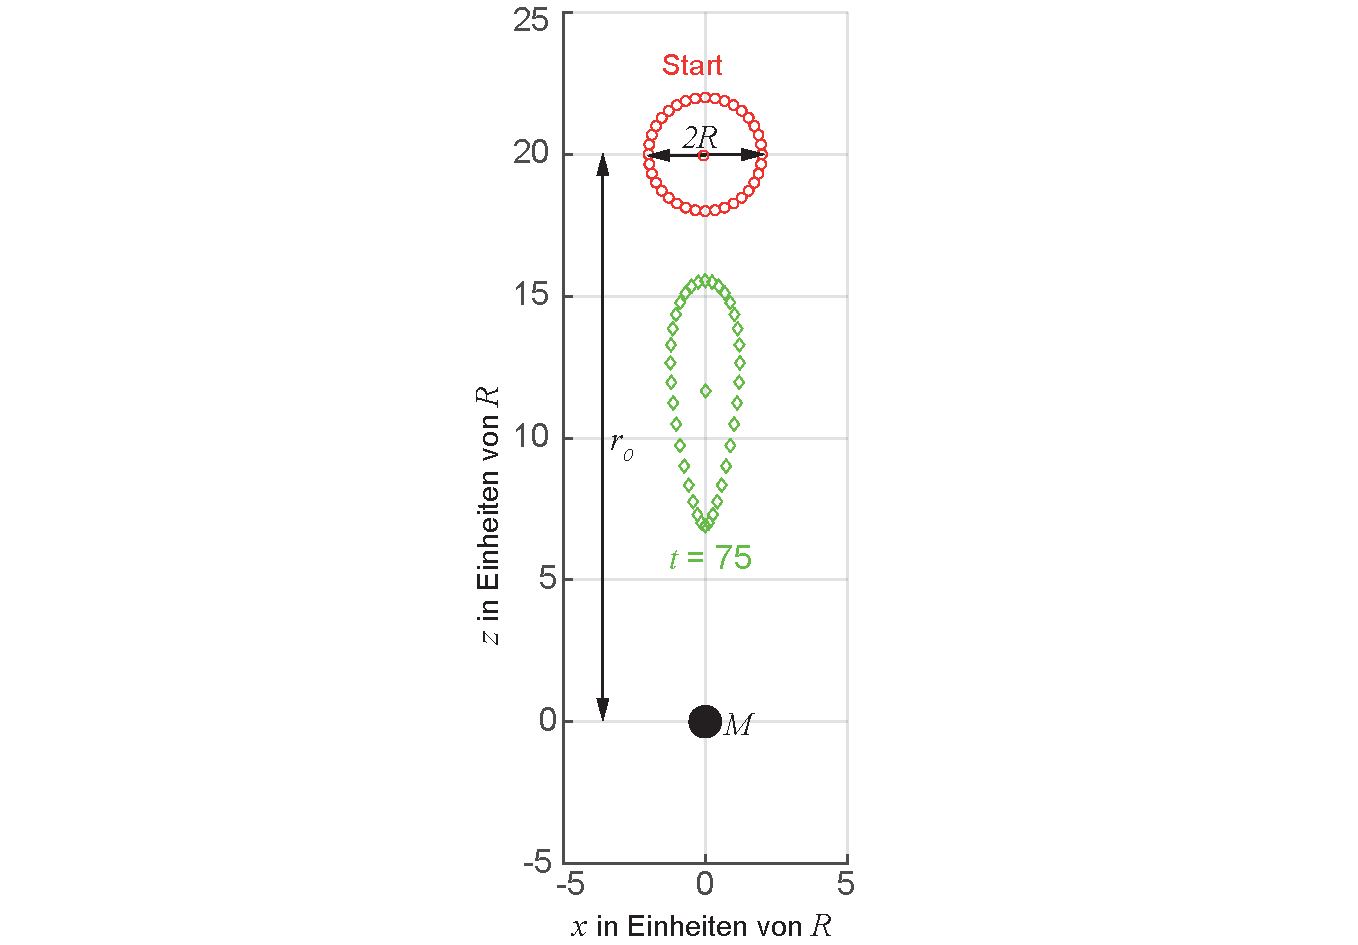
\includegraphics[width=\textwidth]{Gezeitenkraefte.pdf}
\caption[Gezeitenwirkung auf einen Ring.]{Gezeitenwirkung auf einen Ring aus 36 Massepunkten. Parameter: $r_0 = 20 R, R = 2, M\,G = 1.$}
\label{abb:hm_gezeiten01}
\end{figure}

Das Auseinanderbrechen von Himmelsk�rpern kann man durch die \emph{Roche-Grenze}
\footnote{�douard Albert Roche (1820 -- 1883) war ein franz�sischer Astronom und Mathematiker, der vor allem mit seinen theoretischen Arbeiten wichtige Beitr�ge zur Himmelsmechanik lieferte. 1850 berechnete er die nach ihm benannte kritische Distanz $r_\text{R}$, bei der ein Satellit unter der Wirkung von Gezeitenkr�ften zerrissen wird.}\index{Roche-Grenze}\index{Roche-Limit|textbf}\indexp{Roche, �douard Albert} (englisch \textit{Roche-Limit}) beschreiben.
Die Roche-Grenze ist die Entfernung eines Himmelsk�rpers der Dichte $\varrho_\text{S}$ von seinem Zentralk�rper der Dichte $\varrho_\text{Z}$ und des Radius $R_\text{Z}$, unterhalb derer der Himmelsk�rper aufgrund der Gezeitenkr�fte zerrissen wird.
Dabei wird angenommen, dass der K�rper nur von den eigenen Gravitationskr�ften zusammengehalten wird.
%Die Roche-Grenze ist damit die kleinste Umlaufbahn, in der der Himmelsk�rper den Zentralk�rper noch stabil umlaufen kann, ohne zerrissen zu werden.
Die Roche-Grenze ist gegeben durch
    \begin{align}
        r_\text{R} = \alpha\,R_\text{Z}\,\lk \frac{\varrho_\text{Z}}{\varrho_\text{S}}\rk^{\frac{1}{3}}\,, \label{eq:hm_rochelimit01}
    \end{align}
worin $\alpha$ ein materialabh�ngiger dimensionsloser Parameter zwischen $0$ und $1$ ist \cite{Bartelmann2015}.
Wir leiten die Beziehung \eqref{eq:hm_rochelimit01} in \probref{hm_rochelimit} her und sch�tzen auch f�r verschiedene Himmelsk�rper ihre Gr��e ab.

\subsection{Gezeiten im Erde-Mond-(Sonne)-System} \label{kap:hm_gezeiten_EM}

Man findet immer wieder etwas verwirrende oder zumindest unklare Darstellungen zu den Gezeiten des Erde-Mond-Systems (siehe dazu auch die Kommentare in Ref. \cite{Sawicki1999}).
Diese resultieren zumeist aus der unsauberen Betrachtung der verwendeten Koordinatensysteme \bzw der Eigenrotation der Erde im Verh�ltnis zur wahren \bzw scheinbaren Bewegung der Himmelsk�rper Mond und Sonne.
Wir wollen daher im Folgenden auf diese Themen besonderen Wert legen. \\
Als erstes wollen wir noch einmal den Ursprung der Gezeitenkr�fte beleuchten.
Im Kapitel Gezeiten des Bandes I hatten wir diese auf einen ausgedehnten K�rper wirkenden Kr�fte aus dem Gravitationspotential eines als Massepunkt angenommenen (da weit entfernten) Himmelsk�rpers hergeleitet.
Wir hatten in dieser Betrachtung im Inertialsystem offen gelassen, wie sich das System bei relativer Bewegung der die Gezeiten erzeugenden Himmelsk�rper zeitlich verh�lt. Das wollen jetzt nachholen.

\subparagraph{\textbf{\anf{Freier Fall} der Erde im Kraftfeld von Mond \bzw Sonne}}

Wir nutzen zun�chst zur physikalischen Beschreibung ein geozentrisches Koordinatensystem (\figref{hm_gezeiten02}), das aber \emph{nicht} mit der Erde mitrotiert und dessen Ursprung sich auf einem Kreis (\probref{hm_gezeiten01}) um den Schwerpunkt des Himmelsk�rper-Erde-Systems (der Himmelsk�rper ist entweder die Sonne oder der Mond) bewegt.
Da das gew�hlte KOS kein Inertialsystem ist, m�ssen alle Punkte der Erde in diesem System eine Scheinkraft $\vec{F}_\text{T}$ (Tr�gheitskraft, siehe Kapitel 1.2.2 im Band I) erfahren, die f�r alle Punkte des (starren) K�rpers gleich gro� ist.
Diese Kraft ist aber nichts anderes als die Schwerkraft, mit der die Erde im gew�hlten KOS "`frei f�llt"'.
Im Schwerpunkt des Erde-Himmelsk�rper-System (das ist der Ursprung des KOS) w�rde diese Tr�gheitskraft genau der Gravitationskraft entsprechen, ein mitbewegter Beobachter w�rde sich an dieser Stelle schwerelos f�hlen.
F�r alle Punkte der Erde wirkt daher als Gesamtkraft im gew�hlten KOS (\figref{hm_gezeiten02})
\begin{align}
    \vec{F}_\text{ges} = \vec{F}_\text{T} + \vec{F}_\text{G} = \vec{F}_\text{Gez} \,. \label{eq:hm_gezeiten11}
\end{align}
Aus Sicht eines Beobachters im nichtrotierenden geozentrischen KOS ist diese Gesamtkraft aus Gravitations- und Tr�gheitskraft also genau die Gezeitenkraft.
Wir k�nnen diese wie folgt aus \figref{hm_gezeiten02} herleiten:
\begin{align}
\begin{split}
    \vec{F}_\text{Gez} &= \frac{G\,M\,m}{r^3}\,\vec{r} - \frac{G\,M\,m}{r'{}^3}\,\vec{r}_\text{HK}~~
    \text{mit} ~~\vec{r}' = \vec{r} + \vec{R} = \vec{r} + R_\text{E}\frac{\vec{R}}{\left|\vec{R}\right|} \; , \\
		 \vec{r}'{}^2 &= \lk \vec{R} + \vec{r}\rk^2 = R^2 + r^2 + 2\,\lk \vec{R}\cdot\vec{r}\rk= \vec{r}'{}^2 = r^2\,\lk 1+\underbrace{\frac{R^2}{r^2}}_{\substack{\approx 0}} + \frac{2\,\vec{R}\cdot\vec{r}}{r^2}\rk \;.
\end{split} \label{eq:hm_gezeiten12}
\end{align}
In der N�herung $R/r \ll 1$ k�nnen wir $1/r'{}^3$ entwickeln:
\begin{align*}
    \frac{1}{ r'{}^3} = \lk  \vec{r}'{}^2\rk^{-\frac{3}{2}} \approx \lek r^2\lk 1+2\,\frac{\lk \vec{R}\cdot\vec{r}\rk}{r^2}\rk\rek^{-\frac{3}{2}} \approx \frac{1}{r^3}\,\lk 1-\frac{3}{\killA{2}}\,\killA{2}\frac{\lk \vec{R}\cdot\vec{r}\rk}{r^2}\rk \,.
\end{align*}
Damit ergibt sich: 
\begin{align}
     \vec{F}_\text{Gez} &\approx -\frac{G\,m\,M}{r^3}\,\lek \lk \vec{r} + \vec{R}\rk\,\lk 1-3\,\frac{\lk\vec{R}\cdot\vec{r}\rk}{r^2} \rk - \vec{r}\rek \approx -\frac{G\,m\,M}{r^3}\,\lk \vec{R} - \frac{3\,\lk \vec{R}\cdot\vec{r}\rk}{r^2} \lk \vec{r} + \vec{R}\rk \rk \,. \label{eq:hm_gezeiten13}
\end{align}
Wir sehen an \eqref{eq:hm_gezeiten13} zwei Dinge.
Zum einem heben sich die Hauptbetr�ge der Gravitationskraft und der Tr�gheitskraft, die proportional zu $\vec{r}/r^3$ sind, auf. Das ist ja genau f�r den freien Fall im Schwerpunkt zu erwarten.
Zum anderen wird nochmals deutlich, dass nur durch das inhomogene Gravitationsfeld ($\vec{F}(\vec{r}') \neq \vec{F}(\vec{r})$) �berhaupt eine Gezeitenkraft auftreten kann. 

\begin{figure}%
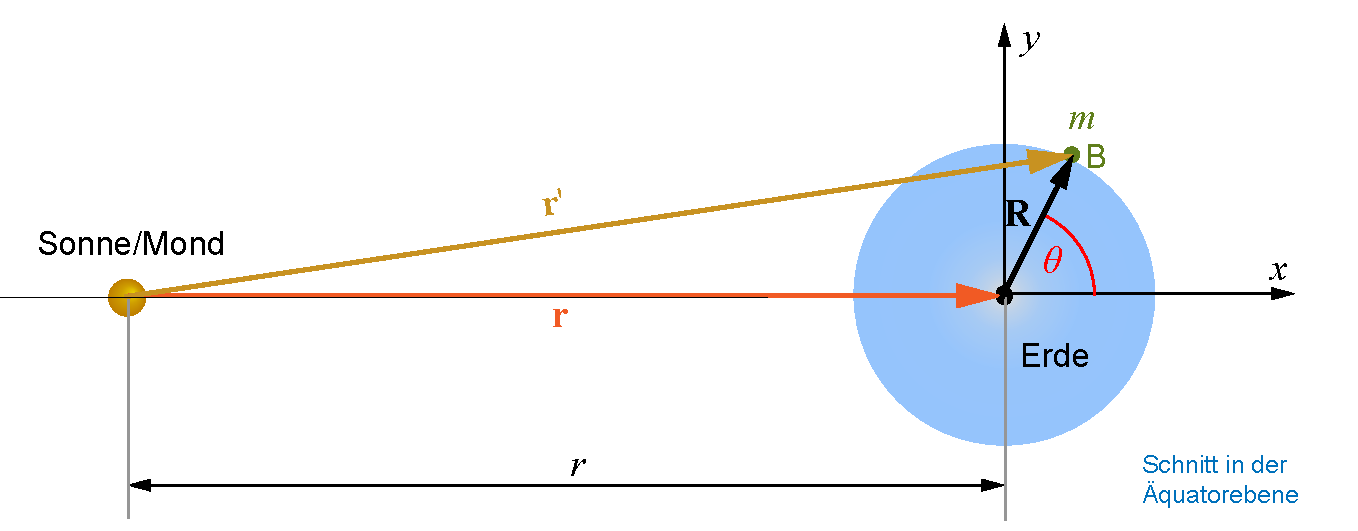
\includegraphics[width=\textwidth]{Gezeiten02.pdf}%
\caption[Zur Berechnung der Gezeitenkr�fte auf der Erdoberfl�che.]{Zur Berechnung der Gezeitenkr�fte auf der Erdoberfl�che (nicht ma�st�bliche Zeichnung). Beim Erde-Mond-System w�rde der gemeinsame Schwerpunkt leicht verschoben in Richtung Mond, aber noch innerhalb der Erde liegen. Die Bahnebenen von Erde und Mond werden vereinfacht als identisch mit der �quatorebene angenommen. B ist der Punkt eines Beobachters an einem beliebigen Punkt des �quators.}
\label{abb:hm_gezeiten02}%
\end{figure}

\subsection{Gezeitentheorie nach Newton}\indexp{Newton, Sir Isaac}\index{Gezeitentheorie nach Newton}\label{kap:hm_gezeiten:Newton}

\subparagraph{\textbf{Gleichgewichtsannahme in der Betrachtung einer nichtrotierenden Erde}}

\begin{figure}%
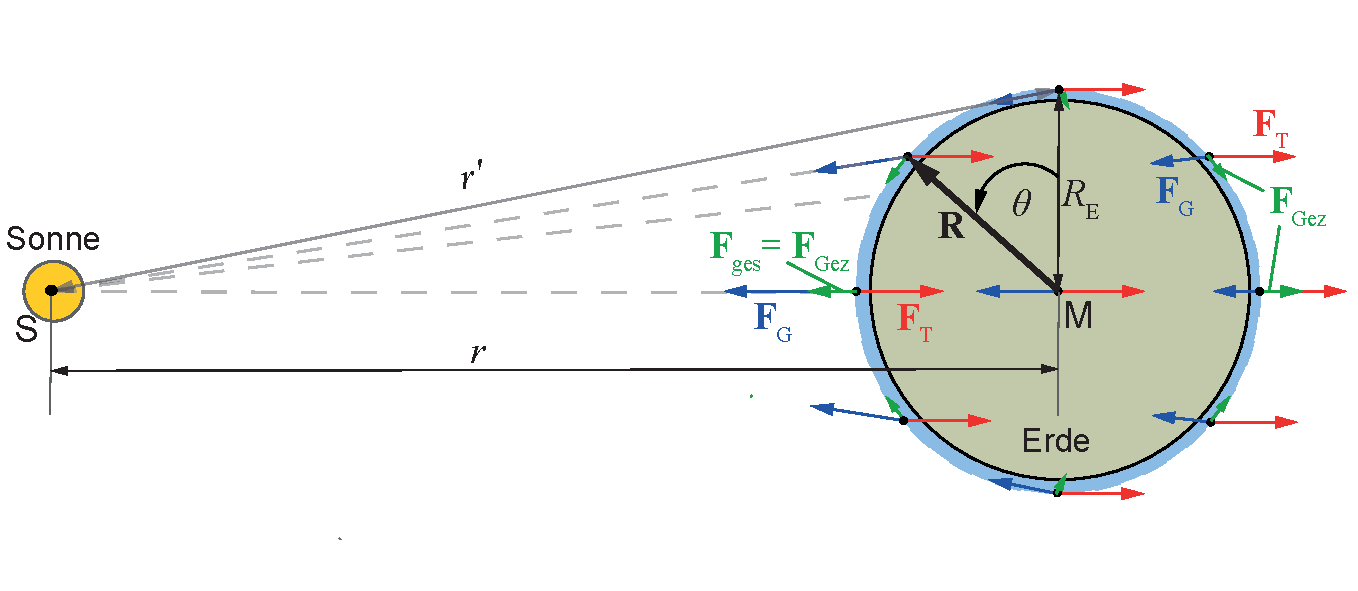
\includegraphics[width=\textwidth]{Gezeiten03S.pdf}%
\caption[Vektorielle Darstellung der Gezeitenkr�fte auf der Erdoberfl�che.]{Vektorielle Darstellung der Gezeitenkr�fte auf der Erdoberfl�che. In jedem Punkt der Erdoberfl�che wird die Vektorsumme aus Gravitations- und Tr�gheitskraft gebildet. Letztere ist �berall gleich gro� (nicht ma�st�bliche Zeichnung). Im Mittelpunkt der Erde heben sich die Kr�fte auf. Beim Erde-Mond-System w�rde der gemeinsame Schwerpunkt leicht verschoben in Richtung Mond, aber noch innerhalb der Erde liegen, an diesem w�rde ebenfalls die Gezeitenkraft verschwinden.}
\label{abb:hm_gezeiten03}%
\end{figure}

Wir betrachten nun, aus Sicht eines Beobachters auf der Erde, die vertikalen und horizontalen Komponenten\footnote{Aus Sicht eines Beobachters im Inertialsystem sind das die radialen \bzw tangentialen Komponenten.} der Gezeitenkraft \bzw der Gezeitenbeschleunigung\footnote{An Gleichung \eqref{eq:hm_gezeiten13} kann man erkennen, dass $F_\text{Gez} \approx \lk \vec{R}\cdot\vec{r}\rk r^{-5}$ ist, was auf ein Quadrupolpotential\index{Quadrupol} f�r die Gezeitenkraft hinweist.\index{Multipolentwicklung} Wir werden uns mit der Multipolentwicklung von Feldern und anderen physikalischen Gr��en in \kap{hm_potentialtheorie}, sowie in der Astrodynamik (Kap. \ref{chap:adyn}) und in der Elektrodynamik (Band IV) besch�ftigen. Hier gen�gt zu wissen, dass eine Quadrupolgr��e dadurch gekennzeichnet ist, dass ihr Potential eine $r^{-5}$-Abh�ngigkeit hat und in zwei zueinander orthogonalen Richtungen auf Grund des Skalarproduktes $\lk \vec{R}\cdot\vec{r}\rk$ unterschiedliche funktionale Abh�ngigkeit von einem Parameter wie \zb dem Winkel zwischen $\vec{R}$ und $\vec{r}$ zeigt.} (\figref{hm_gezeiten03}). Diese k�nnen mit dem Winkel $\theta$ und $\left|\vec{R}\right| = R_\text{E}$ und $g_0= G\,M/r^2$ wie folgt geschrieben werden:
\begin{align}
    g_\text{Gez,H} &= \frac{F_\text{Gez,H}}{m} = -3\,\frac{G\,\killA{m}\,M}{\killA{m}\,r^3}\,R_\text{E}\,\cos\theta\,\sin\theta 
		                =-\frac{3}{2}\,g_0\,\frac{R_\text{E}}{r}\,\sin 2\theta \,. \label{eq:hm_gezeiten14}
\end{align}
Analog folgt f�r die vertikale Komponente aus \eqref{eq:hm_gezeiten13}
\begin{align}
    g_\text{Gez,V} &= +g_0\,\frac{R_\text{E}}{r}\lk 3\cos^2\theta-1\rk = \frac{3}{2}\,g_0\,\frac{R_\text{E}}{r}\lk \cos2\theta+\frac{1}{3}\rk \,. \label{eq:hm_gezeiten15}
\end{align}
Der letzte Term gibt einen konstanten, vom Winkel $\theta$ unabh�ngigen Beitrag $\lk \frac{1}{2}\,g_0\,\frac{R_\text{E}}{r}\rk$ zur Erdbeschleunigung $g_0$ und ist f�r die weitere Betrachtung irrelevant.
Wir k�nnen also n�herungsweise schreiben:
\begin{align}
    g_\text{gez,V} \approx \frac{3}{2}\,g_0\,\frac{R_\text{E}}{r}\,\cos 2\theta \,. \label{eq:hm_gezeiten15a}
\end{align}

Die Erdbeschleunigung $g_\text{E}$ ist durch $g_\text{E} = G\,m_\text{E}/R_\text{E}{}^2$ gegeben, daher k�nnen wir f�r das maximale Verh�ltnis der Gezeitenbeschleunigung zur Erdbeschleunigung schreiben:
\begin{align}
\begin{split}
    \text{Mond:} ~~~~ \left|\frac{g_\text{Gez,M}}{g_\text{E}}\right| 
		 &= \frac{3}{2}\,\frac{m_\text{M}}{m_\text{E}}\,\frac{R_\text{E}{}^3}{r_\text{EM}{}^3} = \frac{3}{2}\,\xi_\text{M}\, R_\text{E} \approx \SI{8.4e-8}{} \,,\\
    \text{Sonne:} ~~~~\left|\frac{g_\text{Gez,S}}{g_\text{E}}\right| 
		 &= \frac{3}{2}\,\frac{m_\text{S}}{m_\text{E}}\,\frac{R_\text{E}{}^3}{r_\text{ES}{}^3} = \frac{3}{2}\,\xi_\text{S}\, R_\text{E}\approx  \SI{3.9e-8}{} \,.
\end{split} \label{eq:hm_gezeiten16}
\end{align}
Hierin ist 
\begin{align}
	  \xi_\text{M} = \frac{m_\text{M}}{m_\text{E}}\,\frac{R_\text{E}{}^3}{r_\text{EM}{}^3} = \frac{m_\text{M}}{m_\text{E}}\,\frac{R_\text{E}{}^3}{a_\text{EM}{}^3} \approx \SI{5.62e-8}{} \label{eq:hm_xi_gezeiten}
\end{align}
ein Ma� f�r die Gezeitenst�rke des Mondes und analog $\xi_\text{S}$ f�r die Sonne, wobei wir f�r $r_\text{EM}$ den Abstand der Mittelpunkte von Erde und Mond $a_\text{EM}$ gesetzt haben.  Die Gezeitenkr�fte betragen also nur weniger als das $10^{-7}$-fache der Erdbeschleunigung, k�nnen aber dennoch durch ihre Horizontalkomponenten eine gro�e Wirkung auf die Ozeane aus�ben.%
\footnote{Man liest immer wieder, dass die Tiden durch \anf{Anheben} des Wassers, \dh die Vertikalkomponente entstehen. Das ist nach \eqref{eq:hm_gezeiten16} wohl kaum m�glich!}
Das erkannte auch schon Newton.
Er nahm f�r die nicht rotierende Erde an, dass die Gezeitenkr�fte wegen der relativ langsamen Bewegung der die Gezeiten erzeugenden Himmelsk�rper eine station�re Form der Wasseroberfl�che der Ozeane ausbilden k�nnen. F�r eine im Gleichgewichtsfall ausgeformte Wasserh�lle muss die Oberfl�che so sein, dass durch die Oberfl�chenverformung die Horizontalkomponente der Gezeitenkraft kompensiert wird. Eine entsprechende Rechnung (siehe \kap{hm_potentialtheorie}) zeigt, dass die so geformte Wasserh�lle ein Ellipsoid der Form 
\begin{align} 
    R_\text{W}\lk \theta \rk = R_\text{E}\,\lk 1 - \frac{2}{3}\,\varepsilon\, \mathcal{P}_2 \lk \cos \theta \rk \rk = R_\text{E}\,\lk 1 - \frac{2}{3}\,\varepsilon \ \lk \frac{3}{2} \cos^2 \theta - \frac{1}{2} \rk \rk \, \label{eq:hm_gezeiten17a}
\end{align}
ergibt, worin $R_\text{E}$ der mittlere Erdradius ist, der n�herungsweise gleich dem Radius der ungest�rten Wasserh�lle der weltumspannenden Ozeane $R_\text{W,0}$ gesetzt wird $(R_\text{E} \approx R_\text{W,0})$.  $\mathcal{P}_2 \lk \cos \theta \rk$ ist das Legendre-Polynom 2.\,Ordnung (siehe \kap{hm_potentialtheorie} und die \onlineZ) und $\varepsilon$ die Elliptizit�t (Abplattung) des Ellipsoids. Diese ist definiert �ber
\begin{align}
	\varepsilon = \frac{R_\text{A} - R_\text{P}}{R_\text{E}} \,, \label{eq:hm_gezreibung03}
\end{align}
worin $R_\text{A},\, R_\text{P}$ die  Radien der Erde am �quator \bzw am Pol (Richtung Symmetrieachse) bedeuten, wie man leicht �berpr�fen kann. 
H�ufig wird die Abh�ngigkeit des Radius von $\theta$ auch n�herungsweise in der Form 
\begin{align} 
    R_\text{W}\lk \theta\rk \approx R_\text{E}\,\lk 1 + \frac{h}{R_\text{E}}\,\cos 2\theta \rk  \label{eq:hm_gezeiten17}
\end{align}
geschrieben, worin $h$ die Anhebung der Wasserh�lle durch die Gezeitenkr�fte ist. 
Wir bestimmen aus \eqref{eq:hm_gezeiten17} den Neigungswinkel $\gamma$ der Wasseroberfl�che als Funktion des Winkels $\theta$ relativ zur Lotlinie.\footnote{Hier nehmen wir implizit an, dass die Dichte des Ozeanwassers verschwindend gering ist und es bleibt zun�chst auch unber�cksichtigt, dass sich der feste Erdk�rper ebenfalls durch die Gezeiten verformt.} Wir erhalten:
\begin{align}
  \gamma &\approx \tan \gamma = \frac{g_\text{Gez,H}}{g_\text{E}} = -\frac{2h}{R_\text{E}}\,\sin 2\theta ~~\rightarrow ~~ \varepsilon = -\frac{2\,h}{R_\text{E}} = -\frac{g_\text{Gez,H}}{g_\text{E}}\,. \label{eq:hm_gezeiten_epsilon}
\end{align}
Offensichtlich ist $\varepsilon < 0$ was mit der Definition eines prolaten Ellipsoiden �bereinstimmt. Die Wasserh�hen durch die Gezeitenkr�fte von Mond und Sonne sind dann:
\begin{align}
\begin{split}
    \Delta h_\text{M} &= 2h_\text{M} = \frac{3}{2}\,\xi_\text{M}\,R_{E} \approx \SI{0.54}{\metre} ~~\text{bzw.} ~~\Delta h_\text{S} = 2h_\text{S} = \frac{3}{2}\,\xi_\text{S}\,R_{E}{} \approx \SI{0.24}{\metre} \,.
\end{split} \label{eq:hm_gezeiten18}
\end{align}

\begin{figure}%
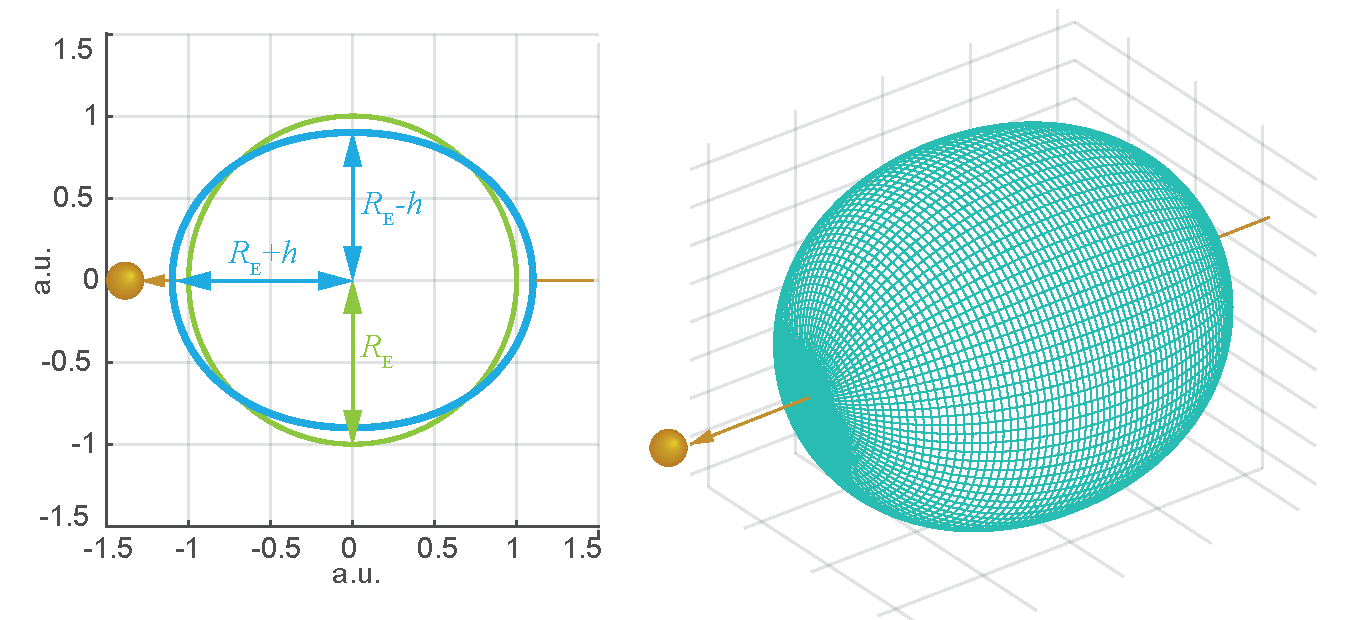
\includegraphics[width=\textwidth]{Gezeiten05.pdf}%
\caption[Gezeitenellipsoid.]{Gezeitenellipsoid. Stark �berh�hte Darstellung, mit $h \approx 0.1 R_\text{E}$. F�r die realen Gezeiten der Ozean auf der Erde ist $h < \SI{1e-7}{}R_\text{E}$.}
\label{abb:hm_gezeiten05}%
\end{figure}

\figref{hm_gezeiten05} zeigt das sich ausbildende Ellipsoid nach Gleichung \eqref{eq:hm_gezeiten17}.
Eine genaue Rechnung zeigt, dass bei einer Annahme der Form der Wasserh�lle nach \eqref{eq:hm_gezeiten17} das Volumen der Wasserh�lle nicht exakt konstant ist, was der Annahme einer inkompressiblen Fl�ssigkeit widerspricht. Da $\Delta h \ll R_\text{E}$ ist die N�herung f�r unsere Rechnungen aber sehr gut zu verwenden. Wir verweisen auch auf die \textbf{�bungen} \ref{prob:hm_gezeiten01} und \ref{prob:hm_gezeiten04}.

\subparagraph{\textbf{Ber�cksichtigung der Eigenrotation der Erde}}

Bisher haben wir nur die Bewegung von Erde und Mond um den gemeinsamen Schwerpunkt in unseren Betrachtungen ber�cksichtigt.%
\footnote{Im Folgenden beziehen wir uns, wenn nicht anders erw�hnt, nur noch auf den Mond. Alle �berlegungen gelten aber prinzipiell genauso f�r die Sonne.}
Danach w�re der Hochwasser-Berg nach Newtons Annahme der instantanen Ausbildung des Gezeitenellipsoids immer auf der Linie Schwerpunkt-Mondmittelpunkt fixiert (\probref{hm_gezeiten01}).
Es w�rde sich daher nur zweimal alle 27.32 Tage Hochwasser und Niedrigwasser ergeben, n�mlich jeweils beim oberen und unteren Meridiandurchgang des Mondes%
\footnote{Man �berlege sich, warum wir die synodische Umlaufzeit des Mondes $(T_\text{synod} = 27.32\,\mathrm{d})$ verwenden m�ssen!}.
Ber�cksichtigen wir jetzt die Erdrotation, wandert die Erdoberfl�che sozusagen st�ndig unter den Hochwasser-Bergen und Niedrigwasser-T�lern in �stlicher Richtung davon, oder bewegt sich anders gesprochen der Hochwasser-Berg in westlicher Richtung um die Erde.\\
F�r die mathematische Beschreibung wechseln wir nun in ein echtes mitrotierendes geozentrisches Koordinatensystem.
Der Winkel $\theta$ wird dann zeitabh�ngig und \ia eine Funktion $\theta(\alpha\lk t\rk, \delta\lk t\rk)$, worin $\alpha$ und $\delta$ die Rektaszension \bzw die Deklination des Mondes sind.
Wir wollen zun�chst der Einfachheit halber eine Deklination des Mondes von $\delta = 0 $ annehmen, \dh der Mond steht �ber dem �quator im Zenit.
Auch an \eqref{eq:hm_gezeiten14} erkennt man, dass es wegen der $\sin 2\theta$--Abh�ngigkeit zwei Hochwasser-Tiden pro Tag geben muss.
Beim Mond muss man die Eigenbewegung ber�cksichtigen, die immerhin $360\degree / 27.32\,\mathrm{d} = 13.177\degree/ \mathrm{d}$ betr�gt.
Im Mittel (Kreisbahn des Mondes angenommen) ist deshalb der Mondtag um $\SI{50}{\min}\,\SI{24}{\second}$ l�nger als der Sonnentag, weswegen der mittlere zeitliche Abstand zwischen zwei Hochwasser ca. $\SI{12}{\hour}\,\SI{25}{\min}$ betr�gt.
Man kann auch sagen, dass ein Pegelstab eines Beobachters quasi in $\SI{24}{\hour}\,\SI{50}{\min}$ einmal durch die ann�hernd station�re Wasserh�lle \anf{pfl�gt} (\probref{hm_gezeiten03}).
In \figref{hm_gezeiten04} haben wir die Wirkung der Horizontalkomponenten auf die Ozeanh�lle der Erde noch einmal schematisch dargestellt.\\

\begin{figure}%
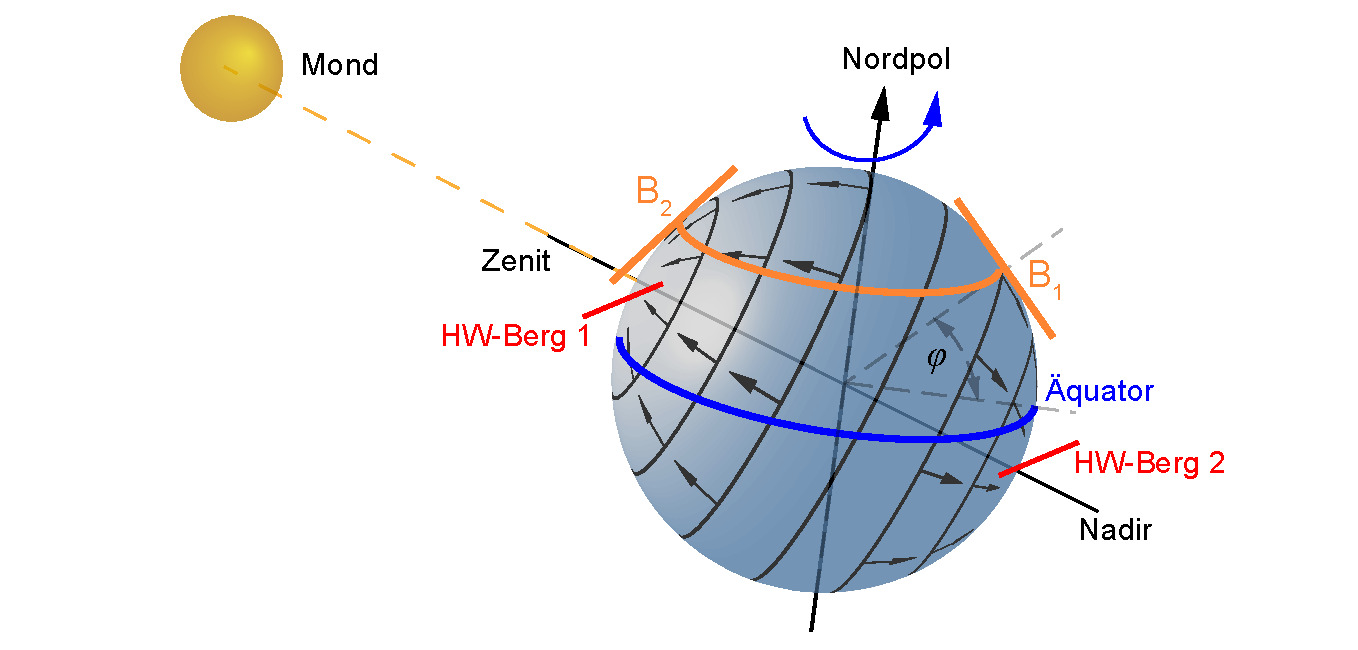
\includegraphics[width=\textwidth]{Gezeiten04.pdf}%
\caption[Gezeiten des Mondes auf der Erde.]{Gezeitenwirkung des Mondes auf der Erde. Ohne Erddrehung w�rde sich nur zweimal alle 27.32 Tage Hochwasser und Niedrigwasser ergeben, n�mlich jeweils beim oberen und unteren Meridiandurchgang des Mondes. Mit Erddrehung ergibt sich nach der Newtonschen Gleichgewichtstheorie pro Tag f�r einen Beobachter auf einen Breitenkreis $\varphi$ zwei Hochwasser und zwei Niedrigwasser, letztere werden durch einen Niedrigwasser-Ring um die Polachse herum gebildet. Man erkennt auch, dass die aufeinanderfolgenden Hochwasserst�nde f�r die Beobachter $\mathrm{B}_1$ und $\mathrm{B}_2$ \ia unterschiedlich gro� sind.}
\label{abb:hm_gezeiten04}%
\end{figure}

Die Newtonsche Gezeitentheorie liefert trotz ihrer Einfachheit schon viele grundlegende richtige Ergebnisse.
Insbesondere lassen sich die Ph�nomene von Spring- und Nipptiden durch unterschiedliche Stellungen von Erde, Mond und Sonne zueinander erkl�ren, ebenso wie die sogenannten astronomisch bedingten "`Ungleichheiten"', die durch Exzentrizit�ten und Neigungen der Bahnen von Erde und Mond erkl�rt werden k�nnen. (\probref{hm_gezeiten03}).
Die absolut berechneten H�hen $\SI{54}{\centi\metre}$ f�r Mondtide \bzw $\SI{24}{\centi\metre}$ f�r maximale Sonnentide gelten aber bestenfalls im freien Ozean, fern von K�sten und selbst da nur eingeschr�nkt.

Nicht erkl�rbar ist durch die Newtonsche Theorie auch, dass die tats�chlich beobachteten Hochwasser-Zeiten nicht, wie nach der Theorie zu erwarten, mit den Kulminationszeiten des Mondes �bereinstimmen. Wir m�ssen also die Theorie verbessern, was wir in \kap{hm_gezeiten_Laplace} beschreiben wollen. 
Zun�chst werden wir aber mit der Potentialtheorie eine breit anwendbare Methode kennenlernen, mit der wir auch noch einmal die Ergebnisse der Newtonschen Gezeitentheorie elegant herleiten wollen und die wir anschlie�end im \kap{hm_gezeitenreibung} sehr vorteilhaft anwenden k�nnen.

\newpage
\subsection{Grundlagen der Potentialtheorie der Gravitation} \label{kap:hm_potentialtheorie}

\subsubsection{Gravitationspotential einer beliebigen Masseverteilung} \label{kap:hm_pot_general_distrib}

Wir wollen zun�chst die grundlegende Beziehung f�r die Berechnung eines Gravitationspotentials einer beliebigen Massenverteilung herleiten. Im Kapitel Physik der Bewegung (Band I) hatten wir dargestellt, wie die Gravitationskraft zwischen zwei Massepunkten aus dem Gravitationspotential berechnet werden kann.
Wir betrachten dazu eine beliebige Anzahl von Massepunkten $m_i \lk i=1\ldots N\rk$. Wir stellen uns vor, dass man nach und nach alle Massen aus dem Unendlichen in eine Anordnung bringt, nach der die Massen $m_i$ jeweils an den Orten $\vec{r}_i$ liegen. Dabei wird durch die Gravitationskraft Arbeit verrichtet werden, die da erstere konservativ ist als Differenz eines Potentials geschrieben werden kann:
    \begin{align*}
        W_i = m_i\,\bigintsss\limits_\infty^{\vec{r}_i}\vec{\nabla}U \cdot \D\vec{s}_i = m_i\lek U\lk \vec{r}_i\rk - \underbrace{U\lk\infty\rk}_{=0}\rek\,.
    \end{align*}
Als gravitative Selbstenergie $U_\text{S}$ aller Massen $m_i$ kann die Summe der Arbeiten $W_i$ verstanden werden. Bei der Doppelsummenbildung muss man einen Faktor $\frac{1}{2}$ anwenden, damit bei der Summe �ber $i$ und $j$ die einzelnen Arbeiten nicht doppelt gez�hlt werden.\footnote{Beispiel f�r 3 Massen: Wir bringen zun�chst die Masse $m_1$ an die Position $\vec{r}_1$, dann $m_2$ an die Position $\vec{r}_2$, schlie�lich $m_3$ an die Position $\vec{r}_3$. Da aber die Reihenfolge egal ist, addieren wir die Arbeiten $W_\text{A} = W_1(\vec{r}_1)+W_2(\vec{r}_1,\vec{r}_2)+W_3(\vec{r}_1,\vec{r}_2,\vec{r}_3) \text{und} W_\text{B} = W_1(\vec{r}_1)+W_3(\vec{r}_1,\vec{r}_3)+W_2(\vec{r}_1,\vec{r}_3,\vec{r}_2)$ und halbieren $W_\text{A}+W_\text{B}$.}
    \begin{align*}
        E_\text{S} &= -\frac{1}{2}\,G\,\sum_{\substack{i,j=1\\i\neq j}}^N\,\frac{m_i\,m_j}{|\vec{r}_i-\vec{r}_j|} = \frac{1}{2}\sum_{i=1}^N W_i = \frac{1}{2}\sum_{i=1}^N m_i\,U_i \\ 
     & \text{mit}~~~ U_i\lk \vec{r}_j\rk = -G\sum_{\substack{j=1 \\ i\neq j}}^N \frac{m_j}{|\vec{r}_i-\vec{r}_j|}\,. 
    \end{align*}
    Von der Summe f�r $U_i\lk \vec{r}_j\rk$ kommt man leicht zum Integral f�r eine kontinuierliche Massenverteilung\footnote{Im strengen Sinne erfolgt die Berechnung �ber die Methode der \textit{Greenschen Funktionen}, die wir in der Potentialtheorie f�r elektrische Felder in der Elektrodynamik (Band IV) kennen lernen werden. Siehe auch \cite{Otto2019, Fischer2018} und \cite{Riley2006, Felder2016}}:
    \begin{align}
      U\lk \vec{r}\rk = -G\bigintsss\frac{\varrho\lk\vec{r}'\rk}{|\vec{r}'-\vec{r}|}\,d^3\,\vec{r}' \; . \label{eq:hm_pot_theo01}
    \end{align}
    Dies ist der allgemeine Ausdruck f�r ein Gravitationspotential
    $U\lk \vec{r}\rk$, das durch eine kontinuierliche Massenverteilung
    $\varrho\lk \vec{r}\rk$ hervorgerufen wird
    (\figref{hm_pot_general_distrib}).

    \begin{figure}[H]
	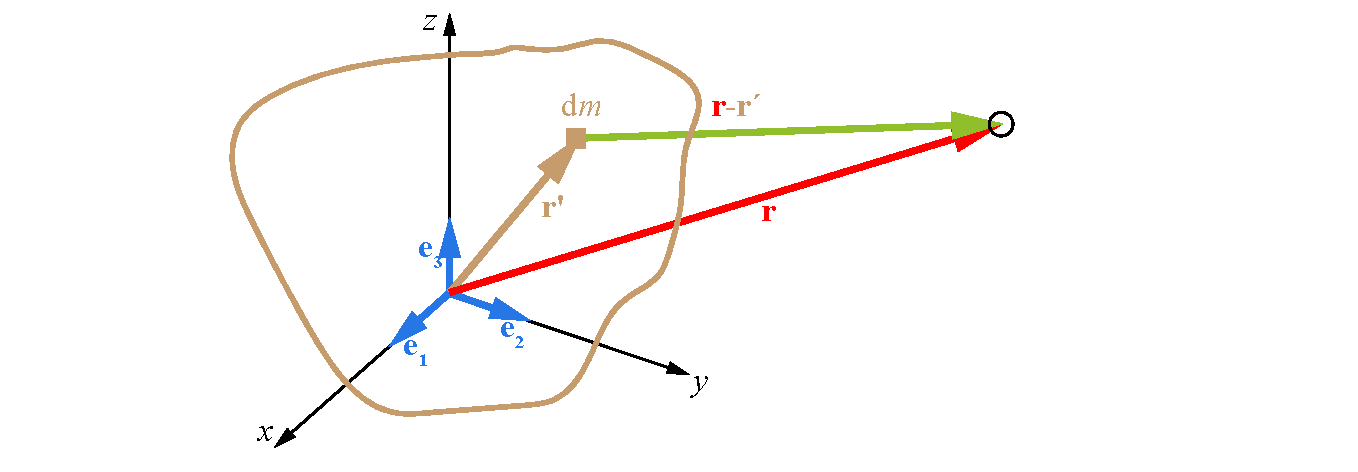
\includegraphics[width=\textwidth]{KOSGravPotential_allg.pdf} 
	\caption[Gravitationspotential f�r kontinuierliche Massenverteilungen.]{Zur Herleitung des Gravitationspotentials f�r kontinuierliche Massenverteilungen.}
	\label{abb:hm_pot_general_distrib}
\end{figure}

\subsubsection{Gravitationspotential einer rotationssymmetrischen Masseverteilung} \label{kap:hm_pot_rotsymm_distrib}

Oft haben wir Massenverteilungen vorliegen, die achsen- \bzw rotationssymmetrisch sind (\figref{hm_pot_rotsymm_distrib}). Die Idee ist nun, mit einer Behandlung des physikalischen Problems in sph�rischen Koordinaten eine angepasste und damit einfachere und elegantere Darstellung zu finden.\\
Wir schreiben \eqref{eq:hm_pot_theo01} in sph�rischen Koordinaten, die wir hier mit $r,\,\phi,\,\theta$ bezeichnen wollen. �ber die Symmetrie-Koordinate $\phi$  kann integriert werden:
    \begin{align}
      U\lk r,\theta\rk = -2\pi\,G\,\bigintsss\limits_0^\infty\bigintsss\limits_0^\pi
      \langle \frac{r'^2\,\sin\theta'\,\varrho\lk r',\theta'\rk}
      {|\vec{r}-\vec{r}'|}\rangle  \,\D r'\, \D\theta' \,,
      \label{eq:hm_pot_theo02} 
    \end{align}

\begin{figure}[H]
	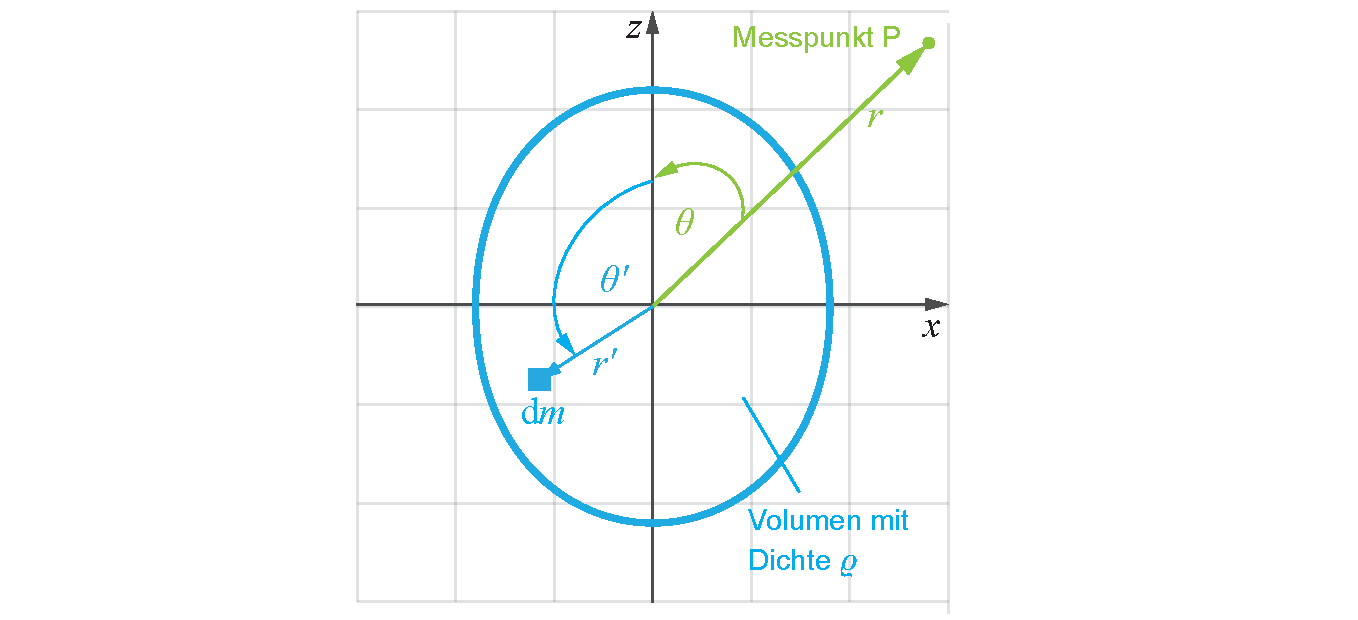
\includegraphics[width=\textwidth]{KOSGravPotential_axial.pdf} 
	\caption[Gravitationspotential f�r rotationssymmetrische Massenverteilungen.]{Zur Herleitung des Gravitationspotentials f�r rotationssymmetrische Massenverteilungen.}
	\label{abb:hm_pot_rotsymm_distrib}
\end{figure}

wobei
    \begin{align}
      \langle \frac{1}{|\vec{r}-\vec{r}'|} \rangle
      = \frac{1}{2\pi}\int\limits_0^{2\pi}\frac{\D\phi'}{|\vec{r}-\vec{r}'|}
      \,\D\phi'\label{eq:hm_pot_theo03} \,,
    \end{align}
eine Mittelung (Integral) �ber die Symmetrie-Koordinate $\phi'$ ist. Wir haben ja bereits mehrfach den Term 
    \begin{align*}
        \frac{1}{|\vec{r}-\vec{r}'|} = \lk r^2-2\vec{r}\,\vec{r}' + r'^2\rk^{-\frac{1}{2}} \,,
    \end{align*}
f�r $|\vec{r}|>|\vec{r}'|$ entwickelt (\zb \eqref{eq:hm_gezeiten12}) und schreiben jetzt das darin auftretende Skalarprodukt $\vec{r}\,\vec{r}'$ als:
    \begin{align}
    \begin{split}
        \vec{r}\,\vec{r}' &= r\,r'\,Q\lk \theta,\theta',\phi'\rk \,, \\
        Q\lk \theta,\theta',\phi'\rk &= \sin\theta\,\sin\theta'\,\cos\phi' + \cos\theta\,\cos\theta' \; ,
    \end{split} \label{eq:hm_pot_theo04}
    \end{align}
woraus folgt:
    \begin{align}
         \frac{1}{|\vec{r}-\vec{r}'|} = &\frac{1}{r} \lek 1 + \frac{r'}{r}\,Q + \frac{1}{2}\,\lk \frac{r'}{r} \rk^2 \lk 3Q^2 - 1 \rk + \mathcal{O} \lk \frac{r'}{r}\rk^3 \rek \,. \label{eq:hm_pot_theo05}
    \end{align}
Wir k�nnen jetzt das Integral \eqref{eq:hm_pot_theo03} gliedweise in \eqref{eq:hm_pot_theo05} ausf�hren und erhalten bis zur zweiten Ordnung in $Q$:
\begin{align*}
  \langle 1 \rangle &= \frac{1}{2\pi}\int\limits_0^{2\pi}\D\phi' = 1\,,\qquad
	\langle Q \rangle = \cos\theta\,\cos\theta' \,,\\
  \langle Q^2 \rangle &= \frac{1}{2}\,\sin\theta\,\sin^2\theta' + \cos^2\theta\,\cos^2\theta' \\
	                    &= \frac{1}{3} +\frac{2}{3}\,\lk \frac{3}{2}\,\cos^2\theta-\frac{1}{2}\rk\lk \frac{3}{2}\,\cos^2\theta'-\frac{1}{2}\rk\,.
    \end{align*}
Damit erhalten wir:
    \begin{align}
        \frac{1}{|\vec{r}-\vec{r}'|} = \frac{1}{r} \bigg[ 1 &+ \frac{r'}{r} \cos\theta\,\cos\theta' \nonumber \\
				       &+ \lk \frac{r'}{r} \rk^2\,\frac{1}{2}\,\lk 3\cos^2\theta-1\rk\,\frac{1}{2}\,\lk 3\cos^2\theta'-1\rk + \mathcal{O} \lk \frac{r'}{r}\rk^3  \bigg] \,. \label{eq:hm_pot_theo06}
    \end{align}
Mit Hilfe der \emph{Legendre-Polynome}\footnote{Adrien-Marie Legendre (1752--1833) war ein franz�sischer Mathematiker, der besonders f�r seine Arbeiten zu den nach ihm benannten Legendre-Polynomen und den elliptischen Integralen bekannt ist.}\indexp{Legendre, Adrien-Marie }\index{Polynome!Legendre-} $\PL n$ (siehe \cite{Riley2006, Felder2016} und die als Anhang \onlineZ), kann man die Beziehung \eqref{eq:hm_pot_theo03} elegant schreiben als:
    \begin{align}
        U\lk r,\theta\rk &= \sum_{n=0}^\infty\Phi_n\lk r\rk\,\PL n\lk \cos\theta\rk\,, \label{eq:hm_pot_theo07}
	  \end{align}
    worin die $\PL n$ durch die \gls{legendrePol} 
    \begin{align}
		\begin{split}
        \PL n\lk \cos\theta\rk =
				\begin{cases}
            1 & n=0 \\
            \cos\theta & n=1 \\
            \frac{1}{2}\,\lk 3\cos^2\theta-1\rk & n=2 \\
            \frac{1}{2}\,\lk 5\cos^3\theta-\cos\theta\rk & n=3 \\
            \ldots & n \geq 4       
				\end{cases}
		\end{split} \label{eq:hm_pot_theo07a}
    \end{align}
gegeben sind und die $\Phi_n\lk r\rk$ durch
    \begin{align}
        \Phi_n\lk r\rk = &-\frac{2\pi\,G}{\lk n+\frac{1}{2}\rk\,r^{n+1}}\,\int\limits_0^r r'^{n+2}\,\varrho_n\lk r'\rk\, \D r' - \frac{2\pi\,G\,r^n}{n+\frac{1}{2}}\,\int\limits_r^\infty r'^{1-n}\,\varrho_n\lk r'\rk \,\D r' \,. \label{eq:hm_pot_theo08}
    \end{align} 
Dabei haben wir folgende Entwicklungen benutzt:
    \begin{align*}
      \text{f�r}~r>r':~~  \frac{1}{|\vec{r}-\vec{r}'|} &= \frac{1}{r} \sum\limits_{n=0}^\infty \lk \frac{r'}{r}\rk^n \PL n(\cos\theta)\, \PL n(\cos\theta')\,~~\text{\bzw} \\
      \text{f�r}~r<r':~~  \frac{1}{|\vec{r}-\vec{r}'|} &= \frac{1}{r'} \sum\limits_{n=0}^\infty \lk \frac{r}{r'}\rk^n \PL n(\cos\theta)\, \PL n(\cos\theta')\,.
		\end{align*}
Die Beziehung \eqref{eq:hm_pot_theo08} k�nnen wir auch schreiben als:
		\begin{align*}
        \Phi_n\lk r\rk = \,&T_{1n}\lk r\rk + T_{2n}\lk r\rk \,. 
    \end{align*}
Dabei haben wir mit 
    \begin{align}
        \varrho\lk r',\theta'\rk = \sum_{n=0}^\infty \varrho_n\lk r'\rk\,\PL n\lk \cos\theta'\rk \label{eq:hm_pot_theo09}
    \end{align}
eine Entwicklung der Dichtefunktion nach \gls{legendrePol} verwendet, was immer m�glich ist, da die $\PL n$ ein vollst�ndiges Orthonormalsystem bilden \cite{Riley2006, Felder2016}. Mit \eqref{eq:hm_pot_theo07} bis \eqref{eq:hm_pot_theo09} haben wir also folgendes erreicht:
    \begin{enumerate}
        \item [1.] Wir haben die Variablen $\theta$ und $r$ (\bzw $\theta'$ und $r'$) jeweils separiert. 
        \item [2.] Wir haben eine Reihenentwicklung mit Ordnungen von ${r'}/{r}$ \bzw ${r}/{r'}$ errhalten.
        \item [3.] Wir konnten den Radialanteil $\Phi_n(r)$ in zwei Anteile $T_{1n}$ und $T_{2n}$ separieren, wobei die Anteile $T_{2n}$ nur relevant sind, wenn man das Potential innerhalb der Massenverteilung berechnen will.
		\end{enumerate}
Wir werden im Folgenden an zwei Spezialf�llen verdeutlichen, wie man mit den Beziehungen \eqref{eq:hm_pot_theo07} und \eqref{eq:hm_pot_theo08} das Potential $U(\vec{r})$ berechnet. 

\subsubsection{Gravitationspotential f�r zwei Spezialf�lle} \label{kap:hm_pot_special cases}

\subparagraph{\textbf{Homogene Kugel mit Dichte $\hat{\varrho}_0$ und Radius $R$ }}

Es gilt, da keine Winkelabh�ngigkeit vorliegt:
\begin{align*}
  \varrho_0\lk r'\rk
  &= \begin{cases}
    \hat{\varrho}_0 & r'\leq R \\
    0 & r'> R
  \end{cases} ~~\text{und}~~\varrho_n\lk r'\rk = 0 ~~~~ \forall\, n \geq 1\,.
\end{align*}
Dann folgt f�r $r>R$:
\begin{align*}
  T_{10} &= -\frac{4\pi\,G}{r}\,\int\limits_0^R \hat{\varrho}_0\,{r'}^2\,\D'r = \frac{4\pi\,G}{r}\,\frac{1}{3}\,\hat{\varrho_0}\,R^3 = -\frac{M\,G}{r}\,,\quad
  T_{20} &= 0 \,, \\
  \rightarrow ~~~~ U\lk r\rk &= -\frac{M\,G}{r} \,,
\end{align*}
was wir nat�rlich schon wussten. Das Gravitationspotential einer Kugel ist au�erhalb der Kugel gleich dem eines Massepunktes, der die gleiche Masse $M$ wie die Kugel hat und in deren Zentrum liegt. F�r $r \leq R$ (innerhalb der Kugel) gilt:
\begin{align}
  T_{10} &= -\frac{4\pi\,G\,\hat{\varrho}_0}{r}\,\frac{1}{3}\,r^3 \,,~\quad 
  T_{20} = -4\pi\,G\,\hat{\varrho}_0\,\lk \frac{R^2}{2}-\frac{r^2}{2} \rk \,,\nonumber \\
  U&= -\frac{4\pi\,G\,\hat{\varrho}_0\,R^3}{3R}\,\lk \frac{3}{2}-\frac{3r^2}{2R^2} + \frac{r^2}{R^2}\rk = -\frac{M\,G}{R}\,\lk \frac{3R^2-r^2}{2R^2}\rk \,. \label{eq:hm_pot_theo10}
\end{align}
% 
\subparagraph{\textbf{Homogener Rotationsellipsoid}}

				Der Rotationsellipsoid hat die Dichteverteilung
				\begin{align*}
						\varrho\lk \theta'\rk = \hat{\varrho}_0\,\lk 1-\frac{2}{3}\,\varepsilon\,\PL 2\lk \cos\theta'\rk\rk \, ~~\text{und}~~ \varepsilon = \frac{R_\text{A}-R_\text{P}}{R_0}\,.
				\end{align*}
				Hierin ist $\PL 2\lk \cos\theta'\rk = \frac{1}{2}\,\lk 3\cos\theta'-1\rk$ und $R_0$, $R_\text{A}$, $R_\text{P}$ sind der mittlere, der �quatoriale und der Polradius des Ellipsoids, sowie $\varepsilon$ seine Elliptizit�t.\footnote{Teilweise wird in der Himmelsmechanik die Elliptizit�t �ber die Abplattung leicht anders definiert: $f=\frac{R_\text{A}-R_\text{P}}{R_\text{A}}$. F�r kleine $\varepsilon$ \bzw $f$ stimmen aber die Werte ann�hernd �berein.}
								F�r die Elliptizit�t gilt : 
				\begin{itemize}
				\item $\varepsilon > 0$  bedeutet $R_\text{A} > R_\text{P}$, also ein oblater Ellipsoid mit $R_\text{P} = R_0\lk 1-\frac{2}{3}\,\varepsilon\rk$, $R_\text{A} = R_0\,\lk 1+\frac{1}{3}\,\varepsilon\rk$ \\
				\item $\varepsilon < 0$  bedeutet $R_\text{A} < R_\text{P}$, also ein prolater Ellipsoid mit $R_\text{P} = R_0\lk 1+\frac{2}{3}\,|\varepsilon|\rk$, $R_\text{A} = R_0\,\lk 1+\frac{1}{3}\,\varepsilon\rk$
				\end{itemize} 
				Das Potential nach \eqref{eq:hm_pot_theo07} und \eqref{eq:hm_pot_theo08} erh�lt man bis zur ersten Ordnung in $\varepsilon$ f�r $|\varepsilon| \ll 1$ nach etwas l�ngerer, aber einfacher Rechnung (\probref{hm_gezeiten07}):
				\begin{align}
						U\lk r,\theta\rk = -\frac{G\,M}{r} + \frac{2}{5}\,\varepsilon\,\frac{G\,M\,{R_0}^2}{r^3}\,\PL 2\lk \cos\theta\rk + \mathcal{O}\lk \varepsilon^2\rk \,.\label{eq:hm_pot_theo11}
				\end{align}
				Mit $J_0 = \frac{2}{5}\,M\,{R_0}^2$ (Tr�gheitsmoment einer homogenen Kugel mit Radius $R_0$) kann man f�r das Potential die einfach merkbare Formel schreiben:
				\begin{align}
						U\lk r,\theta\rk = -\frac{G\,M}{r} + \varepsilon\,J_0\,\frac{G}{r^3}\,\PL 2\lk \cos\theta\rk \,.\label{eq:hm_pot_theo12}
				\end{align}
Wir werden bei der Behandlung der Gezeitenreibung (\kap{hm_gezeitenreibung}) die Potentialberechnung f�r Rotationsellipsoide mehrfach verwenden.


\subsection{Grundidee der Gezeitentheorie nach Laplace} \label{kap:hm_gezeiten_Laplace}

Wir wollen jetzt die Grundidee der dynamischen Theorie beleuchten, die eine wesentliche Verbesserung der Newtonschen Theorie darstellt.
Sie wurde origin�r von Laplace\indexp{Laplace, Pierre-Simon (Marquis) de} entwickelt und besteht darin, die Tiden als station�re erzwungene Schwingungen eines schwingungsf�higen Systems der Ozeanbecken anzunehmen. \\
Das einfachste Modell dazu geht auf Airy zur�ck.%
\indexp{Airy, George Biddell}\footnote{Sir George Biddell Airy (1801 -- 1892) war ein englischer Mathematiker, Physiker und Astronom, der wichtige Beitr�ge zur Himmelsmechanik und besonders auch zur Optik lieferte.}
Er nahm f�r ein Gedankenexperiment an, dass sich die Gezeiten wie Wassermassen in einem breiten Kanal gro�er Wassertiefe entlang des Erd�quators bewegen und periodisch angeregt werden.
In einem solchen Kanal w�rde das Wasser also st�ndig hin- und zur�cklaufen, es werden sich stehende Oberfl�chen-Wellen (siehe Physik des Kontinuums, Band I) ausbilden. 
Diese stehenden Wellen haben wegen der gro�en Wassertiefe $h_\text{T}$ eine Wellenl�nge $\lambda$, die etwa dem halben Erdumfang entspricht.
Die sich um den �quator bewegende Welle hat  eine elliptische Form.
% ist nicht 2.65 gemeint?
Man kann das auch so formulieren, dass sich die beiden Hochwasser-Berge in \figref{hm_gezeiten05} mit dieser Welle um den Erdball bewegen.
Wir wollen nun auf Basis dieses vereinfachten Bildes zeigen, dass damit die beobachtete zeitliche Verschiebung des Hochwasser vom Kulminationspunkt des Mondes erkl�rt werden kann.
Wir erinnern uns, dass die Periode der vom Mond erzeugten Gezeiten durch
\begin{align*}
    \frac{2\pi}{\omega_\text{Gez}} = T_\text{Gez} = &\,\SI{12}{\hour}\,\SI{25}{\minute} \,
\end{align*}
gegeben ist. Die Periode einer Oberfl�chenwelle bei einer Wassertiefe $h_\text{T}$ und einer Wellenl�nge $\lambda$ von etwa dem halben Erdumfang $(\approx \pi\,R_\text{E})$ ist gegeben durch (siehe Kapitel2 im Band I)
\begin{align*}
    \frac{2\pi}{\omega_\text{Welle}} = T_\text{Welle} = \frac{\lambda}{c_\text{Welle}} \approx \frac{\pi\, R_\text{E}}{\sqrt{g\,h_\text{T}}} \approx \,\SI{30}{\hour}\,,
\end{align*}
worin $c_\text{Welle} = \sqrt{g\,h_\text{T}}$ die Ausbreitungsgeschwindigkeit der Wellen ist.
Wir wissen aus dem Kapitel �ber Oszillatoren im Kap. 1.3.2 (Band I), dass bei erzwungenen Schwingungen diese mit der Frequenz der Erregerschwingung schwingen, die Amplitude und Phasenlage aber von der D�mpfung und dem Verh�ltnis von Erregerfrequenz (hier $\omega_\text{Gez}$) zur Eigenfrequenz (hier $\omega_\text{Welle}$) abh�ngen.
Da die beiden zeitlich um $\SI{12}{\hour}\,\SI{25}{\min}$ versetzten Gezeiten-Erregerschwingungen ann�hernd die gleiche Amplitude und Frequenz haben und die Eigenfrequenz und die D�mpfung f�r die beiden stehenden Wasserwellen auch als gleich angenommen werden kann, wird auch die �berlagerung eine feste Phasenbeziehung zu der die Gezeiten erzeugenden Funktion haben.
Ebenso wissen wir aus der Behandlung von Pendelbewegungen, dass die Phase der erzwungenen Schwingung bei geringer D�mpfung gegeben ist durch
\begin{enumerate}
    \item [a)] $\Delta\varphi = 0$, falls Erzeugerfrequenz kleiner als Eigenfrequenz, \dh in unserem Fall \bzw \\
    $T_\text{Gez} > T_\text{Welle}$
    \item [b)] $\Delta\varphi=\pi$, falls Erzeugerfrequenz gr��er als Eigenfrequenz, \dh in unserem Fall $T_\text{Gez} < T_\text{Welle}$
\end{enumerate}
F�r unser einfaches Modell gilt offensichtlich Fall b.
Somit erkl�rt dieses einfache Bild eine beobachtete Phasenverschiebung zwischen Kulmination und Hochwasser-Zeitpunkt.
Bedingt durch die Reibung wird die Phasenlage aber von $\pi$ abweichen.\footnote{Nat�rlich gibt es auch Gezeitenwirkungen (\zb Deformationen) im Erdk�rper selbst.
Die Eigenfrequenz ist aber viel gr��er als $\omega_\text{Gez}$, ebenso ist die D�mpfung viel st�rker, weswegen die beobachtete Verzerrung der Gesteinsh�lle der Erde ann�hernd an der Erd-Mond-Linie ausgerichtet (\ca $3\degree$) ist.} In \probref{hm_gezeiten06} wollen wir ein sehr einfaches mathematisches Modell der gerade dargestellten Grundz�ge der dynamischen Theorie behandeln. \\
In unseren Betrachtungen zur dynamischen Theorie haben wir \zt stark vereinfachende Annahmen gemacht.
Das Schwingungssystem ist nat�rlich viel komplexer als ein Kanal um den �quator, so dass der Ansatz von Airy von Henri Poincar�\indexp{Poincar�, Jules Henri}, Joseph Proudman, Arthur Doodson\indexp{Proudman, Joseph}\footnote{Joseph Proudman (1888--1975) und Arthur Thomas Doodson (1890--1968) waren britische Ozeanographen und Mathematiker, die sich mit der Theorie der Gezeiten befassten.}\indexp{Doodson, Arthur Thomas} und anderen weiterentwickelt wurde.
Danach entstehen durch die Gezeitenkr�fte stehende Wellen\index{Wellen!stehende}\index{Knoten} in den Ozeanen mit Knoten, in denen die Amplitude sehr gering ist aber die Str�mungsgeschwindigkeit entsprechend gro� (\figref{hm_gezeiten06}).
Als Folge der Coriolis-Kraft\index{Coriolis-Kraft} (im Kapitel 1.2.2 (Band I)) entstehen dadurch kreisende bis elliptische Bewegungen um diese ann�hernd station�ren Knotenpunkte.
Solche rotierende Gezeitenwellen haben stets einen \emph{amphidromischen Punkt} (\emph{Amphidromiepunkt})\index{Amphidromiepunkte} mit Amplitude 0, um den mindestens ein "`Hochwasser-Berg"' und ein "`Niedrigwasser-Tal"' herumlaufen.
Man kann sich das sehr sch�n veranschaulichen durch eine waagerecht gelagerte Fahrradfelge, die einen Schlag hat.
Die Nabe, der Amphidromiepunkt, hat immer dieselbe (Meeres-)H�he, aber der Felgenrand geht hoch und runter.
Ein typisches Beispiel f�r eine rotierende Gezeitenwelle ist die Nordsee, in der die Wellenl�nge wegen der geringeren Wassertiefe kleiner ist und es dadurch mehrere Amphidromiepunkte in relativ geringem Abstand gibt (\figref{hm_gezeiten06a}, \probref{hm_gezeiten03}).\\
Zusammengefasst besteht nach der dynamischen Theorie das schwingungsf�hige System also aus einer Reihe ozeanischer Bassins, die unterschiedlich aneinander gekoppelt sind.
Jedes hat seine charakteristische Eigenfrequenz und Reibung (bedingt durch Wassertiefe, Uferformation, Temperatur).
Obwohl das ganze System gut eingeschwungen ist, gibt es durch die Variationen in den erzeugenden Gezeitenkr�ften immer wieder Unregelm��igkeiten, die die theoretische Berechnung der Gezeiten sehr schwierig macht.
Deshalb sind rein theoretische Vorhersagen f�r Orte der Erde auf Basis der dynamischen Theorie praktisch nicht m�glich, obwohl man in den letzten Jahren mit entsprechenden Gro�rechnern enorme Fortschritte gemacht hat \cite{Woodworth2019, Lyard2021}.

\begin{figure}%
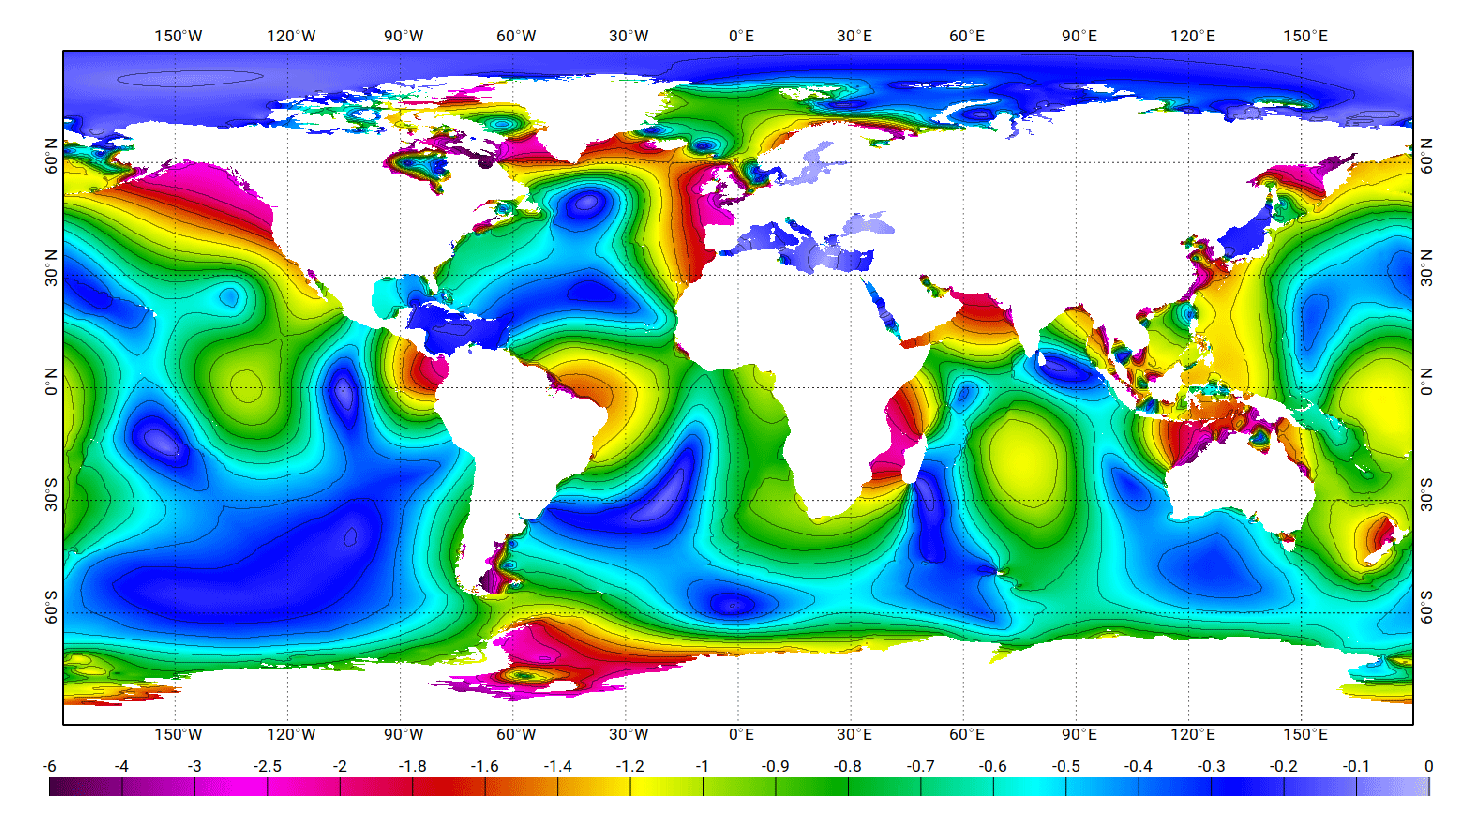
\includegraphics[width=1.1\textwidth]{TidalMaps01.pdf}%
\caption[Amplitude der $M_2$-Tide nach einem numerischen Modell.]{Amplitude f�r die $M_2$-Tide nach einem numerischen Modell \cite{Lyard2021}. Deutlich zu erkennen sind unter anderen die Amphidromiepunkte im Pazifik und im S�datlantik.}
\label{abb:hm_gezeiten06}%
\end{figure}

\begin{figure}%
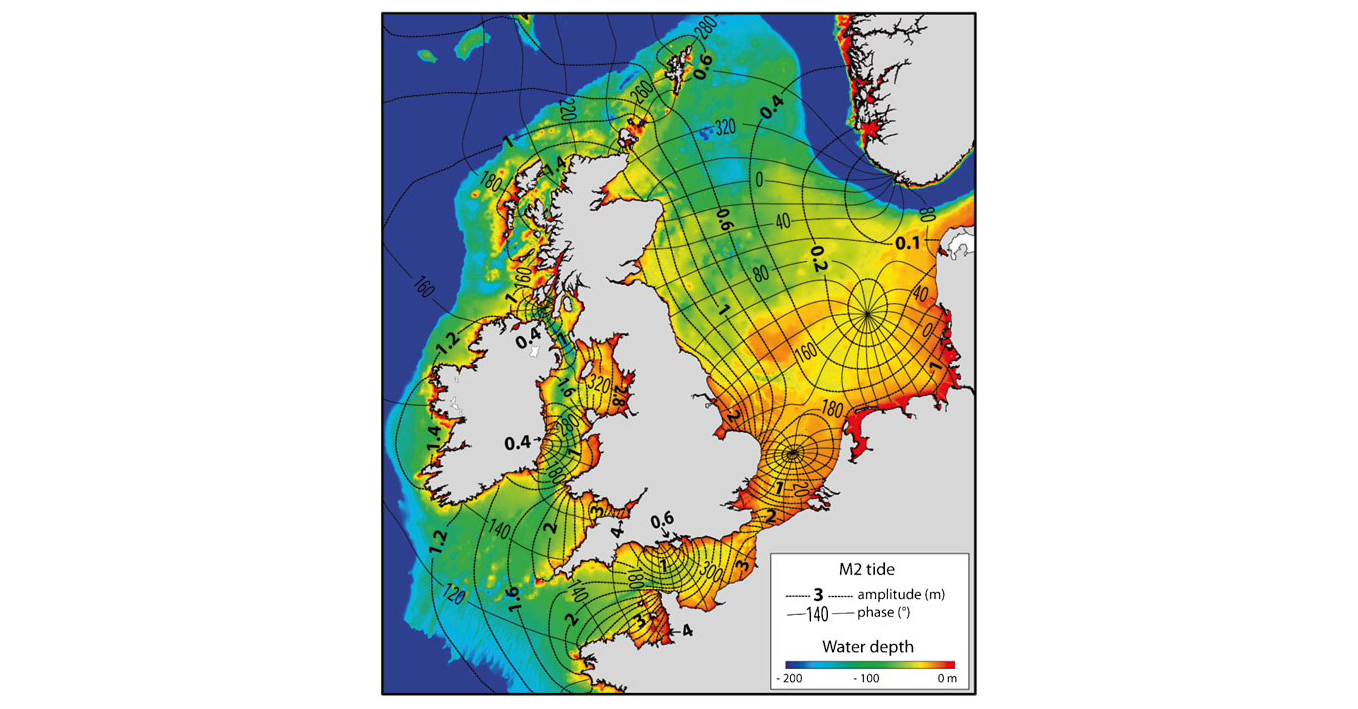
\includegraphics[width=1.2\textwidth]{TidalMaps01a.pdf}%
\caption[Amplitude und Phase der $M_2$-Tide f�r die Nordsee.]{Amplitude und Phase f�r die $M_2$-Tide in der Nordsee mit deutlich erkennbaren Amphidromiepunkten (experimentelle Werte). \cite{Reynaud2012}. Siehe auch \probref{hm_gezeiten03}.}
\label{abb:hm_gezeiten06a}%
\end{figure}

F�r die Seefahrt und andere Anwendungen werden mit gro�em Aufwand Gezeitentafeln publiziert.
Diese beruhen auf der sogenannten harmonischen Analyse von Langzeitbeobachtungen, denen die Annahme zugrunde liegt, dass das Gezeitenverhalten eine �berlagerung von Schwingungen mit Perioden (und Vielfachen der Perioden) von Mond und Sonne darstellt.
Diese periodischen Abh�ngigkeiten sind �berall auf der Welt gleich.
Nur die Einzelphasen und Einzelamplituden (und D�mpfungen) der entstehenden Schwingungen unterscheiden sich von Standort zu Standort.
Heute kann man mit \ca 20--40 der dominanten harmonischen Komponenten (die st�rksten sind die halbt�gliche Mondtide $M_2$ und die halbt�gliche Sonnentide $S_2$) schon sehr gute Vorhersagen machen, da ohnehin die �berlagerung durch lokale Effekte wie Wind, Luftdruck, Erw�rmung, Str�mungs�nderungen Vorhersagen von genauer als auf einen Zentimeter wenig sinnvoll sind. Man beschr�nkt sich daher auf Zentimeter-Genauigkeit.\footnote{Vor dem Aufschwung der digitalen Rechentechnik wurden Gezeitenvorhersagen mit imposanten mechanischen Rechnern durchgef�hrt, heute nat�rlich auf \textit{High-Performance Computern} (HPC).
Selbst auf dem PC kann man heute schon sinnvolle Berechnungen anstellen.}\\
Nachdem wir die Physik der Gezeiten auf der Erde nach den beiden Grundmodellen behandelt haben, wollen wir testen, wie die Ergebnisse mit realen Messungen �bereinstimmen.
Wegen der genannten Komplexit�t und geographischen Besonderheiten ist nicht zu erwarten, dass brauchbare Ergebnisse aus den einfachen theoretischen Rechnungen \zb f�r die Nordsee oder die Atlantikk�ste erzielt werden k�nnen.
Wir haben uns daher die Gezeitentafel in der N�he des �quators f�r Diego Garcia im Indischen Ozean f�r eine �bung herausgesucht (\probref{hm_gezeiten06}), um die Theorie zumindest ansatzweise �berpr�fen zu k�nnen.
Zur Vertiefung dieses komplexen Themas empfehlen wir \ua die Referenzen \cite{Butikov2001, Butikov2014, Weyer2012, Melchior1966, Norsen2017}.

\subsection{Gezeitenreibung}\label{kap:hm_gezeitenreibung}\index{Gezeitenreibung}

\subparagraph{\textbf{Ph�nomenologische Betrachtung}}

In \probref{hm_erdrotation} hatten wir untersucht, wie man aus den Beobachtungsdaten von Sonnenfinsternissen �ber mehrere tausend Jahre schlie�en  kann, dass sich die Erdrotation verlangsamt, \dh die Rotationsperiode $T_\text{P,E}$ gr��er wird.
Es gilt heute als gesichert, dass die Zunahme der Tagesl�nge der Erde etwa $\SI{2.1}{\milli\second}/\mathrm{Jh.}$ betr�gt, was einer Abnahmerate der Rotationsenergie der Erde von 
	\[\frac{\D T_\text{Rot}}{\D t} = \frac{\D}{\D t} \lk\frac{J_\text{E}}{2}\omega^2\rk = \SI{-3.6e12}{\W}
\]
entspricht.
Diese �nderung der Rotationsenergie und des damit verbundenen Drehimpulses muss durch ein Drehmoment der Gr��e
	\[M_\text{D} = \frac{\D}{\D t} \lk {J_\text{E}}\,\omega_\text{E} \rk = \SI{-5.2e16}{\N\metre}\,
\]
hervorgerufen werden \cite{Brosche1989}.
Die ersten Betrachtungen zur Gezeitenreibung gehen auf Halley\indexp{Halley, Edmund} zur�ck.
Immanuel Kant erkannte 1754 als erster die bremsende Wirkung der Meeresgezeiten, jedoch ohne den Zusammenhang zum Mond zu sehen.\indexp{Kant, Immanuel}\footnote{Immanuel Kant (1724 -- 1804) war ein deutscher Philosoph und Professor f�r Logik an der Universit�t K�nigsberg.
Er z�hlt zu den bedeutendsten Philosophen der Geschichte. Mit seiner "`Kritik der reinen Vernunft"' markierte er den Beginn der modernen Philosophie.} Die erste qualitativ richtige Beschreibung lieferte 1848 Robert Mayer%
\indexp{Mayer, Julius Robert von}\footnote{Julius Robert von Mayer (1814 -- 1878) war ein deutscher Arzt und Naturforscher. Er formulierte als einer der ersten Wissenschaftler den Ersten Hauptsatz der Thermodynamik.}, w�hrend 
George Howard Darwin%
\footnote{Sir George Howard Darwin (1845 -- 1912) war ein britischer Astronom und Mathematiker. Er war ein Sohn des ber�hmten Naturforschers Charles Darwin und ist bekannt f�r seine Abspaltungstheorie, nach der der Mond einst Teil der Erde gewesen sein soll.} die Anerkennung f�r die erste vollst�ndige analytische Beschreibung des Problems geb�hrt.\indexp{Darwin, Sir George Howard}\\
Wir werden zun�chst eine einfache ph�nomenologische Beschreibung f�r die Gezeitenreibung geben. Daraus werden wir ein Modell entwickeln, auf dessen Basis wir eine mathematisch-analytische Beschreibung angehen. %, die durchaus mit dem uns zur Verf�gung stehenden mathematisch-physikalischen Instrumentarium m�glich ist.
Wir werden dabei der Einfachheit halber die Gezeitenwirkung der Sonne vernachl�ssigen und nur die Wechselwirkung mit dem Mond in Betracht ziehen.\\
Wir hatten bisher nur �ber die Wirkung der Gezeitenkr�fte auf die Ozeanh�lle gesprochen.
Aber nat�rlich wirken diese auch auf den festen Erdk�rper, der eine gewisse Elastizit�t hat.
Daher wird der Erdk�rper ebenfalls mit phasenverschobenen Oszillationen (seismischen Wellen) auf die Anregung durch die Gezeitenkr�fte antworten, wobei im Gegensatz zu den Ozeanwellen die Eigenfrequenz und die D�mpfung der seismischen Wellen deutlich gr��er sind.
In \kap{hm_gezeiten_Laplace} und \probref{hm_gezeiten05} hatten wir gesehen, dass die �berlagerung dieser Wellen, abh�ngig von deren Eigenfrequenz und D�mpfung zur Ausbildung einer stehenden Welle f�hrt, deren Maximum um einen Winkel $\delta$ phasenverschoben zur Erdmittelpunkt-Mond-Linie ist.
Dabei kommt es im Fall der Erde zu einem vorauseilenden Gezeitenberg ($\delta >0 \approx 3\degree$) (\figref{hm_gezeiten07}).

\begin{figure}%
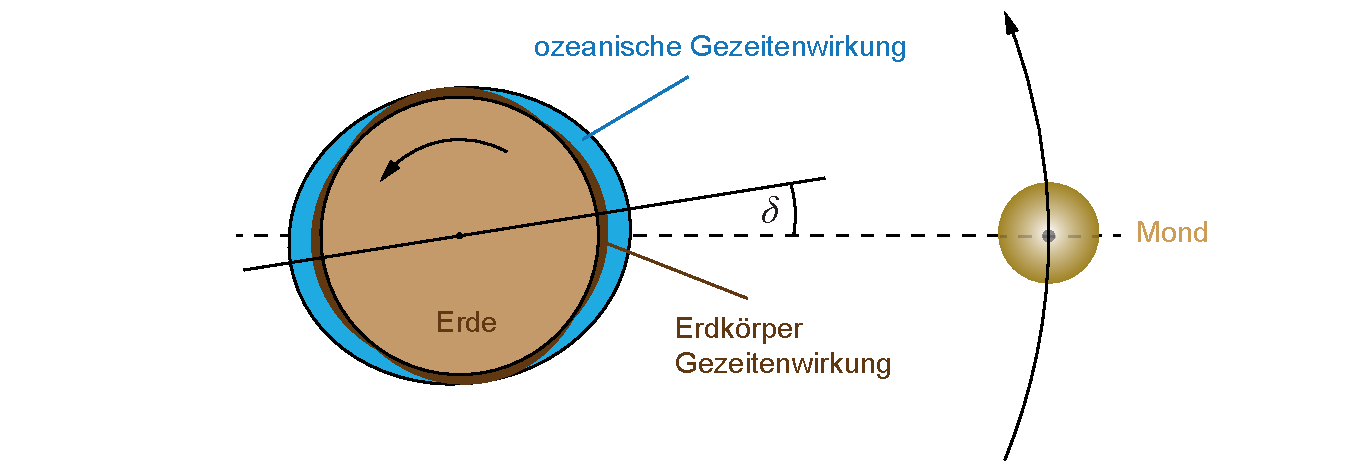
\includegraphics[width=\textwidth]{GezeitenFestOzean.pdf}%
\caption[Gezeitenausbildung im Ozean und im Erdk�rper.]{Gezeitenausbildung im Ozean und im Erdk�rper.}
\label{abb:hm_gezeiten07}%
\end{figure}

Diese von Null verschiedene Phasenlage von Gezeitenberg und Erde-Mond-Linie ist entscheidend f�r das Auftreten von Gezeitenreibung.
Ein vorauseilender Gezeitenberg beschleunigt dabei den Mond und verringert die Erdrotation.
Das kann man sich leicht an \figref{hm_gezeiten08}a klar machen.
Versteht man den Gezeitenberg als Hantel mit Massen an den Punkten A und B, so wird der Mond durch diese in Richtung Hantelkopf A gezogen, also beschleunigt, mithin $\dot{\omega}_\text{M} > 0$.
Da der Effekt im Perig�um \glslink{periapsis} (Erdn�he) am gr��ten ist wird sich auch die Exzentrizit�t der Bahn vergr��ern und folglich $\dot{\omega}_\text{E} < 0$ sein. 
Entsprechend umgekehrt sind die Verh�ltnisse bei einem nachlaufenden Gezeitenberg wie in \figref{hm_gezeiten08}b gezeigt.
Hier wird der Mond ebenfalls in Richtung Hantelkopf A gezogen, mithin verz�gert, folglich ist $\dot{\omega}_\text{M} < 0$ und $\dot{\omega}_\text{E} > 0$. Dabei gilt aber, dass der  die der Gesamtdrehimpuls des Erde-Mond-Systems bleibt erhalten bleibt.
Es ist auch sofort einsichtig, dass es f�r $\delta=0$ keine Beschleunigung oder Verz�gerung geben kann, da das Drehmoment auf Grund der Symmetrie verschwindet.
Entscheidend f�r das Auftreten der Gezeitenreibung ist also ein zeitlicher Versatz des Maximums der Gezeitenellipse zum Meridiandurchgang des Mondes.
Im Fall der Erde f�hrt wie bereits erw�hnt dieser Versatz von \ca $3 \degree$  zu einer experimentell, \zb durch Laserentfernungsmessungen, nachgewiesenen Zunahme des Mondbahnradius von
\begin{equation*}
  \D a_\text{EM}/\D t \approx \SI{4.4}{\cm}/\text{Jahr}\; ,
\end{equation*}
wie wir auch gleich (und auf anderem Weg in \probref{hm_gezeiten06}) nachrechnen wollen.
F�r das Gesamtsystem ist aber keineswegs mechanische Energieerhaltung gegeben, nur ein kleiner Teil (ca. $3\%$) wird von der Mondbahn aufgenommen, der Rest muss in der Erde dissipiert werden.
Wie genau das passiert, ist immer noch ein aktueller Forschungsgegenstand in der Geophysik. 

\begin{figure}%
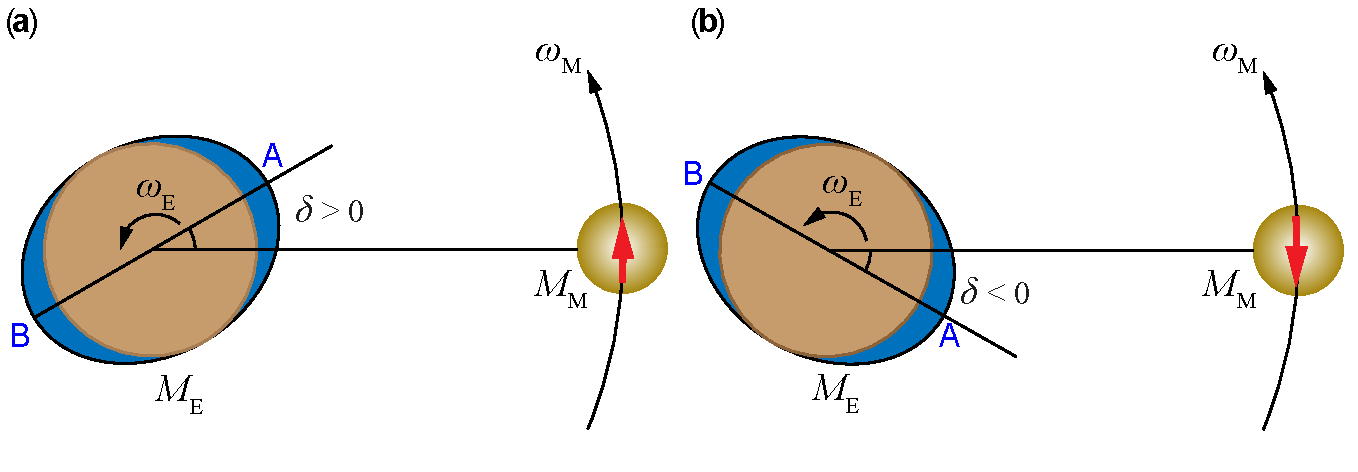
\includegraphics[width=\textwidth]{GezeitenDelay.pdf}%
\caption[Prinzip der Gezeitenreibung.]{Prinzip der Gezeitenreibung. \fa vorlaufender Gezeitenberg, \fb
  nachlaufender Gezeitenberg.}
\label{abb:hm_gezeiten08}%
\end{figure}

\subparagraph{\textbf{Mathematische Beschreibung}}

Wir wollen nun die mathematische Beschreibung angehen.
Das Drehmoment, das vom Mond auf das Gezeitenellipsoid der Erde wirkt, hat als Pendant ein vom Betrag her gleich gro�es aber mit entgegengesetztem Vorzeichen versehenes Drehmoment, das vom Gezeitenellipsoid auf den Mond wirkt.
Dies ist eine direkte Folge der Gesamtdrehimpulserhaltung im Erde-Mond-System. 
Aus dem Winkelversatz $\delta$ berechnet sich ein zeitlicher Versatz $\Delta t =\SI{12}{\minute}$.
%\begin{align}
	%\delta = 360\degree\,\frac{\Delta t}{\SI{24}{\hour}} = 3\degree\,. \label{eq:hm_gezreibung01}
%\end{align}
F�r unsere Rechnungen treffen wir noch einige weitere vereinfachende Annahmen:
\begin{itemize}
   \item Wir vernachl�ssigen, dass der Schwerpunkt des Erde-Mond-Systems um ca. $\SI{4900}{\km}$ vom Erdmittelpunkt verschoben ist und nehmen den Erdmittelpunkt als Zentrum der Mondumlaufbahn.
   \item Der Mond bewegt sich auf einer Kreisbahn mit Radius $a_\text{EM}$ um die Erde.
   \item Der Umlauf des Mondes erfolge in der �quatorebene der Erde und nach dem 3. Keplerschen Gesetz mit der Umlauffrequenz
    \begin{align}
        \omega_\text{M} = \sqrt{\frac{G\,\lk m_\text{E} + m_\text{M}\rk}{a_\text{EM}{}^3}} \,. \label{eq:hm_gezreibung02}
    \end{align}
   \item F�r die gew�hlte Anordnung kann die mit Ozeanen bedeckte Erde ohne Gezeiten als Kugel (Radius $R_\text{E}$) angenommen werden.
   \item Die Erde rotiert mit $\omega_\text{E} =2\pi/T_\text{P,\,E}$.
\end{itemize}
Wir wollen die Wechselwirkung des Gezeitenellipsoids mit dem Mond �ber das Gravitationspotential der Erde (inklusive des Potentials des Gezeitenellipsoids) beschreiben.
In \kap{hm_pot_special cases} \bzw \probref{hm_gezeiten07} hatten wir das Gravitationspotential eines homogenen Rotationsellipsoids berechnet (Gl. \eqref{eq:hm_pot_theo12}). Das k�nnen wir hier verwenden und schreiben bei bekannter Elliptizit�t $\varepsilon$ das Potential dieses durch die Geitenwirkung des Mondes geformten Rotationsellipsoiden folgenderma�en: 
\begin{align}
    U\lk r,\theta\rk = -\frac{G\,M}{r} + \frac{2}{5}\,\varepsilon\,\frac{G\,M\,R^2}{r^3}\,\mathcal{P}_2 \lk\theta\rk  + \mathcal{O}\lk \varepsilon^2\rk \,. \label{eq:hm_gezreibung03a}
\end{align}
Auf die Erde angewandt, bei der die Achse des Rotationsellipsoids um $\delta$ gegen die Erde-Mond-Linie verdreht ist, muss man $\theta$ durch $\theta - \delta$ ersetzen und erh�lt:
\begin{align}
    U\lk r,\theta,\delta\rk = -\frac{G\,m_\text{E}}{r} + \frac{2}{5}\,\hat{\varepsilon} \,\frac{G\,m_\text{E}\,R_\text{E}{}^2}{r^3}\,\lk \frac{3}{2}\cos^2\lk \theta-\delta\rk-\frac{1}{2}\rk \;, \label{eq:hm_gezreibung04}
\end{align}
wobei wir hier mit $\hat{\varepsilon}$ eine allgemeinere Elliptizit�t eingef�hrt haben, die die gesamte elliptische Verformung der Erde durch die Gezeitenkr�fte des Mondes unter Ber�cksichtigung einer teilelastischen Erde beschreibt. 
F�r einen festen K�rper mit einer effektiven Festigkeit\footnote{Die effektive Festigkeit ist eine dimensionslose Gr��e, die sich f�r einen homogenen K�rper aus den Materialeigenschaften berechnen l�sst und f�r die Erde $\approx 3.35$ betr�gt \cite{Fitzpatrick2022}.} $\tilde{\mu}$ findet man \cite{Fitzpatrick2022}:
\begin{align}
\begin{split}
    \hat{\varepsilon}  &= - \frac{15}{4}\,\frac{1}{1+\tilde{\mu}}\, \frac{R_{E}{}^3}{r^3}\,\frac{m_\text{M}}{m_\text{E}} = - \frac{15}{4}\,k\, \frac{R_{E}{}^3}{r^3}\,\frac{m_\text{M}}{m_\text{E}}\,.
\end{split} \label{eq:hm_gezreibung04a}
\end{align}
F�r einen idealen Ozean (mit Dichte 0) hatten wir mit \eqref{eq:hm_gezeiten_epsilon})
\begin{align}
    \hat{\varepsilon}  = -\varepsilon = - \frac{3}{2}\, \frac{R_{E}{}^3}{r^3}\,\frac{m_\text{M}}{m_\text{E}} \label{eq:hm_gezreibung04b}
\end{align}
hergeleitet. Hier haben wir �ber die sogenannte effektive Festigkeit des Planeten $\tilde{\mu}$ etwas vereinfachend die die sogenannte Love\index{Love-Zahl}\footnote{Augustus Edward Hough Love (1863 -- 1940) war ein britischer Mathematiker und Physiker, der besonders auf der Elastizit�tstheorie arbeitete.}\indexp{Love, Augustus Edward Hough}-Zahl $k$ ber�cksichtigt. Sie ist ebenfalls ein dimensionsloser Parameter und ein Ma� f�r die Festigkeit eines K�rpers in Reaktion auf eine Gezeitenkraft und h�ngt von Faktoren wie der Viskosit�t\index{Love-Zahl}\index{Viskosit�t} (siehe Kapitel 2 Band I) und der Reibung ab. Sie ist ein Ausdruck daf�r, dass sich der Gezeitenberg  nicht bis zu seiner theoretisch maximal m�glichen H�he ausbilden wird. Die beiden Gleichungen \eqref{eq:hm_gezreibung04a} und \eqref{eq:hm_gezreibung04b} zeigen im Vergleich, dass die Gezeitenwirkung auf einer teileastischen Erde das $\frac{5}{2} k$-fache der Wirkung auf einen (idealen, masselosen) die Erde umspannenden Ozean betragen. Wir rechnen im Folgenden f�r die Erde  mit einer Love-Zahl $k$ im Bereich von 0.2.

Dann ist das Gravitationspotential des herausgebildeten Rotationsellipsoids der teilelastischen Erde (wir rechnen im weiteren nur mit diesen Werten), das auf den Mond wirkt, gegeben durch:
\begin{align}
    U\lk r,\theta,\delta\rk &= -\frac{G\,m_\text{E}}{r}-\frac{2}{5}\,\frac{15}{4}\,k\,\frac{G\,m_\text{M} \,R_{E}{}^5}{r^6}\,\mathcal{P}_2 \lk\cos(\theta - \delta) \rk \nonumber \\
														&= -\frac{G\,m_\text{E}}{r}-\frac{3}{2}\,k\,\frac{G\,m_\text{M} \,R_{E}{}^5}{r^6}\, \lk \frac{3}{2}\cos^2\lk\theta-\delta\rk - \frac{1}{2}\rk \,.  \label{eq:hm_gezreibung05}
\end{align}
Durch dieses Potential, oder besser gesagt die daraus folgende Kraft, wird ein Drehmoment auf den Mond ausge�bt, was sich in sph�rischen Koordinaten berechnet zu:
\begin{align}
\begin{split}
    \vec{M}_\text{D} &= \vec{r} \times \vec{F}  = - m_\text{M}\,  \vec{r} \times \vec{\nabla}{U} = - m_\text{M}\,\frac{1 \,\d U}{r \,\d \theta} \,r \,\,\vec{e}_r \times \vec{e}_\theta \\
										 &= - m_\text{M}\,\frac{\d U}{\d \theta} \vec{e}_\phi\, |_{\theta=0,r=a_\text{EM}} \,. \label{eq:hm_gezreibung06}
\end{split}
\end{align}
F�r den Betrag des Drehmoments erhalten wir: 
\begin{align}
    \left|\vec{M}_\text{D}\right|  & \approx \frac{9}{2}\,k\,\delta \,\frac{G\,m_\text{M}{}^2}{R_\text{E}}\,\lk \frac{R_\text{E}}{a_\text{EM}}\rk^6\,, \label{eq:hm_gezreibung07} 
\end{align}
wobei wir kleine Winkel angenommen haben ($\sin\delta\approx \delta, \cos\delta\approx 1$). \\
Wie bereits erw�hnt, gibt es nur f�r $\delta\neq 0$ ein Drehmoment.
Wir finden nun die eingangs gemachte �berlegung, wie das Drehmoment wirkt, best�tigt, ein $\delta > 0$ bewirkt eine Beschleunigung des Mondes (und damit eine Verlangsamung der Erdrotation), f�r $\delta<0$ umgekehrt (siehe auch \probref{hm_gezeiten06}).\\
Wir wollen jetzt noch die Gr��enordnungen der Effekte der Gezeitenreibung absch�tzen.
Wir wissen, dass das Drehmoment eine �nderung des Drehimpulses bewirkt.
Da (wie angenommen) die Bewegung in einer Ebene stattfindet, kann sich nur der Betrag des Drehimpulses �ndern.
Wir schreiben f�r die �nderung des Betrages des Erddrehimpulses:
\begin{align}
    \frac{\D}{\D t} L_\text{E} &= \frac{\D}{\D t} (J_\text{E}\,\omega_\text{E}) = - \left|\vec{M}_\text{D}\right|  \,, \nonumber \\ 
		\rightarrow~~\dot{\omega}_\text{E} &= - \frac{\left|\vec{M}_\text{D}\right|}{J_\text{E}} = - \frac{45}{4}\,\frac{G\,m_\text{M}{}^2}{m_\text{E}}\,\frac{R_\text{E}{}^3}{a_\text{EM}{}^6}\,k\,\delta\,.
		\label{eq:hm_gezreibung07a}
\end{align}
Mit dem 3. Keplerschen Gesetz \eqref{eq:hm_gezreibung02} finden wir schlie�lich:
\begin{align}
    \frac{\dot{\omega}_\text{E}}{\omega_\text{E}} &= - \frac{45}{4}\,k\,\delta\,\frac{\omega_\text{M}{}^2}{\omega_\text{E}}\,\frac{m_\text{M}{}^2}{m_\text{E}{}^2}\,\frac{R_\text{E}{}^3}{a_\text{EM}{}^3}\approx \SI{-8e-18}{\per\second}\,.
		\label{eq:hm_gezreibung08}
\end{align}
Mit dieser Abnahmerate der Rotationsgeschwindigkeit erhalten wir eine Verl�ngerung der Rotationsdauer der Erde um
\begin{equation*}
  \Delta T_\text{P,E}=-\frac{\dot{\omega}_\text{E}}{\omega_\text{E}}\,T_\text{PE}\,\,100\, \mathrm{a} \approx \SI{2.17e-03}{\second} \approx \SI{2.2}{\milli\second}
\end{equation*}
pro Jahrhundert.
Die Zeit bis zur synchronen Rotation der Erde betr�gt dann $\Delta T_\text{synch} = \omega_\text{E}/\dot{\omega}_\text{E} \approx \SI{4e+09}{}$ Jahre.\\
Die Drehimpulserhaltung im Erde-Mond-System kann formuliert werden als:
\begin{align}
	L_\text{ges} &=\frac{2}{5}\,m_\text{E}\,R_\text{E}^2\,\omega_\text{E} + m_\text{M}\,a_\text{EM}^2\,\omega_\text{M} = \mathrm{const} \,. \label{eq:hm_gezreibung09}
\end{align}
Ableitung von \eqref{eq:hm_gezreibung09} nach der Zeit und Benutzung von \eqref{eq:hm_gezreibung02} ergibt die Bahnvergr��erungsrate des Mondes zu:
\begin{align}
    \frac{\dot{a}_\text{EM}}{a_\text{EM}} &= -\frac{4}{5}\,\frac{m_\text{E}\, R_\text{E}{}^2}{m_\text{M}\, a_\text{EM}{}^2} \,\frac{\dot{\omega}_\text{E}}{\omega_\text{M}} = C_a  \approx \SI{+3.9e-18}{\per\second} \,, \label{eq:hm_gezreibung10}
\end{align}
was gleichbedeutend mit einer Vergr��erung des Radius der Mondbahn von $ \Delta a_\text{EM} \approx \SI{+4.7}{\metre}$ pro Jahrhundert ist.
Aus der Ableitung von \eqref{eq:hm_gezreibung02} nach der Zeit erh�lt man die Abnahmerate der Umlauffrequenz des Mondes zu $ \dot{\omega}_\text{M}/\omega_\text{M} = -\frac{3}{2}\,C_a \approx \SI{-5.82e-18}{\per\second}$, was wiederum einer Verl�ngerung des synodischen Mondmonats um $\SI{+43}{\milli\second}$ pro Jahrhundert entspricht.\\
Zum Schluss wollen wir noch die Energiedissipation ausrechnen.
Sie ist gleich der vom Drehmoment \eqref{eq:hm_gezreibung07} geleisteten Arbeit pro Zeit:
\begin{align}
   P = \left|\vec{M}_\text{D}\right|\,(\omega_\text{M} - \omega_\text{E}) \approx \SI{-3.90e+12}{\W} \,. \label{eq:hm_gezreibung11}
\end{align}
Die Leistung ist negativ, da $\omega_\text{M} < \omega_\text{E}$ ist.
Sie muss also dissipiert werden.
Die Verlustleistung f�hrt zu einer Erw�rmung der Ozeane und der Erdkruste.
Bei starker Gezeitenreibung, wie sie in anderen Planeten-Mond-Systemen auftritt, kann die Gezeitenerw�rmung zur Verfl�ssigung und vulkanischen Effekten f�hren.
Um ein Gef�hl f�r die Gr��enordnung auf der Erde zu bekommen, geben wir zum Vergleich die gesamte in Deutschland installierte Leistung aller Kraftwerke im Jahre 2022 an: $P_\text{el} = \SI{-2.38e+11}{\W}$ \cite{BNA2022}. Wenn der Zustand der synchronen Rotation erreicht ist, \dh $\omega_\text{M} = \omega_\text{E}$ ist, gibt es auch keine Energiedissipation mehr. 
Alle Berechnungen finden sich im Detail im \mscr{} \mlhmref{Gezeitenreibung01.m}.\\

\subparagraph{\textbf{L�sung der Bewegungsgleichungen}}

Wir wollen jetzt noch kurz beschreiben, wie man das Erde-Mond-System inklusive Gezeitenreibung in seiner zeitlichen Entwicklung numerisch berechnen kann.
Das ist aber nicht ganz so einfach.\footnote{Siehe auch dazu \cite{Schebesta1994}.} Bisher hatten wir die Verdrehung $\delta$ der Gezeitenh�lle als konstant angenommen und daraus das Drehmoment berechnet.
In der Zeitentwicklung wird sich aber $\delta$ verringern bis bei $\delta = 0$ der stabile Endzustand, die gebundene Rotation, erreicht ist.
Das bedeutet, dass das in den Bewegungsgleichungen auftretende Drehmoment von den �ber lange Zeitr�ume sich relativ zueinander ver�ndernden Positionen der Himmelsk�rper abh�ngig ist.
Um die Bewegungsgleichungen f�r Erde und Mond zu erhalten, bilden wir den Gradienten aus dem Potential \eqref{eq:hm_gezreibung05}, das wir als 
	\[U = U_\text{G} + U_\text{Ell}	\,\]
schreiben. Wir benutzen die Koordinatensysteme nach \figref{hm_gezeiten09}.
Der Gradient $\vec{\nabla}_{\vec{r}_\text{E}} U_\text{G}$ erzeugt die Monopolkraft, die auf den Mond wirkt:
\begin{align}
    \vec{F}_\text{G}' \lk \vec{r}_\text{M}'\rk = -G\,m_\text{E}\,m_\text{M}\,\frac{\vec{r}_\text{E}'-\vec{r}_\text{M}'}{|\vec{r}_\text{E}' - \vec{r}_\text{M}'|^3}\,.  \label{eq:hm_gezreibung12}
\end{align}

Bei der L�sung der Bewegungsgleichungen m�ssen wir die Bewegung der beiden Himmelsk�rper um den gemeinsamen Schwerpunkt ber�cksichtigen.
Die mit einem Strich gekennzeichneten Koordinaten sollen  sich auf das Koordinatensystem $\vec{\Sigma}'$ beziehen, dessen Ursprung im gemeinsamen Schwerpunkt der beiden Massen $m_\text{E}$ und $m_\text{M}$ liegt.\footnote{Wir k�nnen die nachfolgenden �berlegungen auch auf ein beliebiges Zweik�rperproblem (Satellit-Zentralk�rper) anwenden, es gilt dann einfach f�r die Indizes E = 1 und M = 2.} Aus dem Potentialanteil der Ellipsoidh�lle $U_\text{Ell}$ berechnet man ebenfalls durch Gradientenbildung die Gezeitenkraft $\vec{F}_\text{Gez}$ die auf den Mond wirkt.
Dabei m�ssen wir beachten, dass die Gezeitenkraft bez�glich des Koordinatensystems $\vec{\Sigma}$ definiert ist, das seinen Ursprung im Massenmittelpunkt der Erde hat (\figref{hm_gezeiten09}).
F�r die Bewegungsgleichungen k�nnen wir aber eine einfache Transformation von $\vec{\Sigma}$ und $\vec{\Sigma}'$ �ber die Translation
\begin{align}
	\vec{r}_\text{M} = \vec{r}_\text{M}' - \vec{r}_\text{E}'  \label{eq:hm_gezreibung12a}
\end{align}
erreichen.
Wir erhalten f�r die Gezeitenkraft im KOS $\vec{\Sigma}$:\\ 
\begin{align}
\vec{F}_\text{Gez}\lk \vec{r}_\text{M}\rk &= m_\text{M}\,\lk -\vec{\nabla}_{\vec{r}_\text{E}}\,U_\text{Ell}\lk \vec{r}_\text{M}\rk\rk \nonumber \\
&= \frac{3}{10}\,k\,G\,m_\text{M}{}^2\,\frac{R_\text{E}^5}{r_\text{M}^*{}^5}\,\lek \frac{6\,\lk \vec{r}_\text{M}^*\cdot \vec{r}_\text{M}\rk}{r_\text{M}{}^5}\vec{r}_\text{M}^* - \lk \frac{15\,\lk \vec{r}_\text{M}^*\cdot\vec{r}_\text{M}\rk^2}{r_\text{M}{}^7} + \frac{3{r_\text{M}^*}^2}{r_\text{M}{}^5}\rk\,\vec{r}_\text{M}\rek \,. \label{eq:hm_gezreibung13}
\end{align}

\begin{figure}%
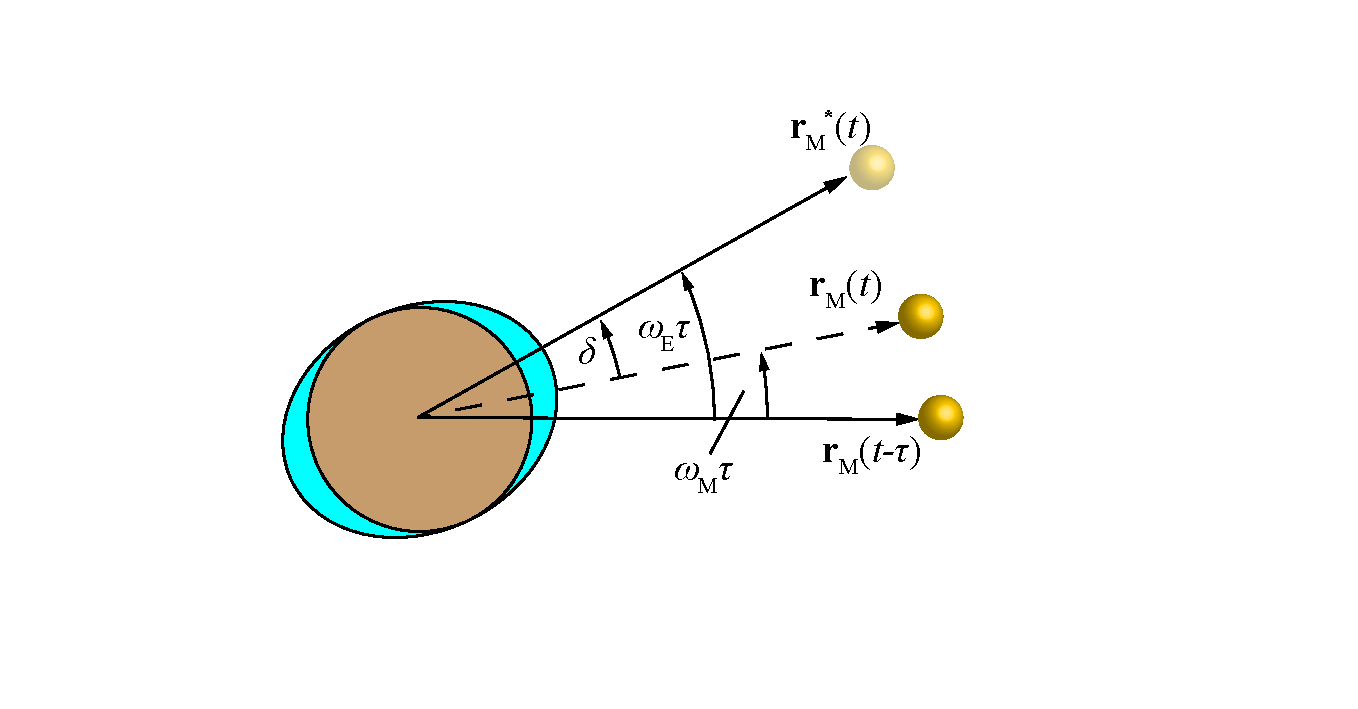
\includegraphics[width=\textwidth]{KOSGezeitenreibung.pdf}%
\caption[Koordinatensysteme der Bewegungsgleichungen der Gezeitenreibung.]{Mitrotierendes Koordinatensysteme $\vec{\Sigma}$ f�r numerische L�sung der Bewegungsgleichungen der Gezeitenreibung zu einer Zeit $t$. Der virtuelle Mond steht im Zenit �ber dem Hochwasser-Berg $\vec{r}_\text{M}^*$, $\vec{r}_\text{M}(t-\tau)$ ist der Ort, an dem ein mitrotierender Beobachter den Mond zur Zeit $t-\tau$ im Zenit gesehen hat. Inzwischen, zur Zeit $t$, befindet sich der Mond aber am Ort $\vec{r}_\text{M}$.}
\label{abb:hm_gezeiten09}%
\end{figure}

Hier haben wir nun einen neuen Vektor eingef�hrt: $\vec{r}_\text{M}^*$. Dies ist der Vektor zum Mond, als dieser kulminierte (\figref{hm_gezeiten09}) oder m.a.W. der Ort des Mondes zu einem Zeitpunkt, als dieser die Gezeitendeformation hervorrief.
Dieser Ort ist aber aufgrund der zeitverz�gerten Antwort der Erde auf die Gezeitenkraft nicht mit dem gegenw�rtigen Ort des Mondes $\vec{r}_\text{M}$ identisch.
Diese Zeitverz�gerung hatten wir mit dem Winkel $\delta \propto \Delta t $ %\eqref{eq:hm_gezreibung01} 
beschrieben.
W�hrend dieser Zeit $\Delta t $ dreht sich die Erde mit $\omega_\text{E}$ um ihre Achse und der Mond mit $\omega_\text{M}$ um die Erde.
Der Zenitalpunkt Z bewegt sich f�r einen Beobachter auf dem  Planeten - im mitrotierenden Koordinatensystem - mit der Winkelgeschwindigkeit $\omega_\text{M} - \omega_\text{E}$.
Wir k�nnen $\vec{r}_\text{M}^*$ auch als die Position eines virtuellen Mondes bezeichnen, der einen instantanen Gezeitenberg erzeugen w�rde.
Der Winkel $\delta$ ist �ber das Skalarprodukt
\begin{align*}
    \vec{r}_\text{M}\cdot\vec{r}_\text{M}^* = |\vec{r}_\text{M}|\,|\vec{r}_\text{M}^*|\,\cos\delta\,.
\end{align*}
mit den beiden Vektoren $\vec{r}_\text{M}$ und $\vec{r}_\text{M}^*$  verkn�pft, die beide im mitrotierenden KOS $\vec{\Sigma}$ definiert sind.

Auf den Schwerpunkt des Mondes wirkt die Summe der Kr�fte $\vec{F}_\text{G}'$ und $\vec{F}_\text{Gez}'$, die Newtonschen Bewegungsgleichungen lauten:
\begin{align}
    m_\text{M}\,\ddot{\vec{r}}_\text{M}' = \vec{F}_\text{G}' + \vec{F}_\text{Gez}'\,. \label{eq:hm_gezreibung14}
\end{align}
Entsprechend gilt f�r den Schwerpunkt der Erde nach dem 3. Newtonschen Axiom:
\begin{align}
    m_\text{E}\,\ddot{\vec{r}}_\text{E}' = -\vec{F}_\text{G}' - \vec{F}_\text{Gez}'\,. \label{eq:hm_gezreibung15}
\end{align}
Wir hatten gesehen, dass die Gezeitenkraft als (r�cktreibendes Moment) auf die Gezeitenh�lle der Erde wirkt.
Die daraus folgende Drehimpuls�nderung wird beschrieben durch:
\begin{align}
    \frac{\D \vec{L}}{\D t} = C\,\dot{\omega}\,\vec{e}_z = -\lk \vec{r}_\text{M} \times \vec{F}_\text{Gez}\rk  
		= \lk r_{\text{M}\,y} \,F_{\text{Gez}\, x}- r_{\text{M}\, x}\,F_{\text{Gez}\, y} 	\rk \,\vec{e}_z  \,. \label{eq:hm_gezreibung16}
\end{align}
Hier haben wir von der Annahme Gebrauch gemacht, dass alle Bewegungen in der $x$-$y$-Ebene stattfinden sollen.%
\footnote{Tats�chlich sind durch die Rotationsabplattung der Planeten (\vgl �bung 1.17 in Band I) die meisten Monde und Kleink�rper in unserem Sonnensystem in unmittelbarer N�he der �quatorebene anzutreffen.}
Mit \eqref{eq:hm_gezreibung10} bis \eqref{eq:hm_gezreibung12} haben wir nun ein Differentialgleichungssystem vorliegen, das uns erlaubt, die zeitliche Entwicklung des Erde-Mond-Systems unter Ber�cksichtigung der Gezeitenreibung zu beschreiben.
Um auch wirklich die Reibung der Gezeiten zu beschreiben, erg�nzen wir die Differentialgleichungen durch einen Reibungsterm proportional zur Geschwindigkeit.
Mit \eqref{eq:hm_gezreibung12a} erhalten wir:
\begin{align}
\begin{split}
    \ddot{r}_{\text{M}\, x}' &= \frac{1}{m_\text{M}}\,\lk   F_{\text{G}\, y}' + F_{\text{Gez}\, x}' - \beta\,|\vec{r}_\text{M}'|\,\dot{r}_{\text{M}\, x}'\rk \,, \\
    \ddot{r}_{\text{M}\, y}' &= \frac{1}{m_\text{M}}\,\lk   F_{\text{G}\, y}' + F_{\text{Gez}\, y}' - \beta\,|\vec{r}_\text{M}'|\,\dot{r}_{\text{M}\, y}'\rk \,, \\
    \ddot{r}_{\text{E}\, x}' &= \frac{1}{m_\text{E}}\,\lk - F_{\text{G}\, x}' - F_{\text{Gez}\, x}' - \beta\,|\vec{r}_\text{E}'|\,\dot{r}_{\text{E}\, x}'\rk \,, \\
    \ddot{r}_{\text{E}\, y}' &= \frac{1}{m_\text{E}}\,\lk - F_{\text{G}\, y}' - F_{\text{Gez}\, y}' - \beta\,|\vec{r}_\text{E}'|\,\dot{r}_{\text{E}\, y}'\rk \,, \\
    \dot{\omega}_\text{E} &= \frac{1}{C}\,\lek \lk r_{\text{M}\,y}'-r_{\text{E}\, y}'\rk\,F_{\text{Gez}\, x} - \lk r_{\text{M}\,x}' - r_{\text{E}\,x}'\rk\,F_{\text{Gez}\, y}\rek \,.
\end{split} \label{eq:hm_gezreibung17}
\end{align}
In den $\vec{F}_\text{Gez}$ \bzw $\vec{F}_\text{Gez}'$  finden wir die Koordinate $\vec{r}_\text{M}^*(t)$.
Die Frage ist, wie man sich diese Koordinate f�r die numerischen Rechnungen beschafft.
Aus Abbildung \figref{hm_gezeiten09} erkennt man, dass f�r ann�hernd kreisf�rmige Bahnen gilt:
\begin{align}
    \vec{r}_\text{M}^*(t) = \mathbb{R}_z(\omega_\text{E}\,\tau)\, \vec{r}_\text{M}(t-\tau) \,, \label{eq:hm_gezreibung18}
\end{align}
worin $\mathbb{R}_z$ die Rotationsmatrix um die $z$-Achse ist.
Im numerischen Programm muss man also eine Routine haben, die alle Orte speichert, an denen der Mond war.
Die numerische Integration von \eqref{eq:hm_gezreibung17} selbst erfolgt aber im raumfesten Schwerpunktsystem $\vec{\Sigma}'$ �ber die Vektoren $\vec{r}_\text{M}'$ und $\vec{r}_\text{E}'$.
Mit der Transformation \eqref{eq:hm_gezreibung12a} und \eqref{eq:hm_gezreibung17} k�nnen wir uns alle Orte $\vec{r}_\text{M}^*(t)$ berechnen und abspeichern, die wir zur numerischen L�sung von 
\eqref{eq:hm_gezreibung17} brauchen.
%Wir geben Hinweise zur relativ komplexen numerische Berechnung in \probref{hm_gezeiten08} an.\\

Mit der Berechnung von Sonnenfinsternissen und der Gezeiten, insbesondere der Gezeitenreibung haben wir so etwas wie die \anf{h�here Schule der Himmelsmechanik} absolviert.
In \figref{hm_gezeiten10} geben wir noch einmal einen graphischen �berblick �ber die wesentlichen Effekt der Mechanik auf unsere Erde.
Es wichtig bei diesen die jeweiligen wirkenden Kr�fte und Koordinatensysteme auseinander zu halten, siehe dazu auch \probref{hm_gezeiten09}.

\begin{figure}[H]
	\includegraphics[width=\textwidth]{VergleichEffekte.pdf} 
	\caption[Vergleich verschiedener Effekte der Himmelsmechanik auf unsere Erde.]{Vergleich verschiedener Effekte der Himmelsmechanik auf unsere Erde. \fa Rotationsabplattung der Erde durch Zentrifugalkraft \fb Pr�zession der Erdachse durch Drehmoment von Mond und Sonne auf die "`�quatorw�lste"' der Rotationsabplattung \fc Gezeitenformation nach der Gleichgewichtstheorie \fd Gezeitenreibung durch Drehmoment des Mondes auf die verdrehte "`Gezeitenh�lle"'.}
	\label{abb:hm_gezeiten10}
\end{figure}



\section{Himmelsmechanik unseres Sonnensystems �ber lange Zeitr�ume}\label{kap:hm_langezeiten}

\subsection{Bahnparameter der Planeten in ihrer zeitlichen Entwicklung}

Bevor wir die Himmelsmechanik endg�ltig verlassen wollen, werfen wir noch einen Blick auf die Entwicklung unseres Sonnensystems �ber lange Zeitr�ume.
Dabei spielen zwei Effekte eine Rolle, zum einen die Ver�nderung der Bahnparameter �ber lange Zeiten, die zu deutlich ver�nderten Konstellationen (z.\,B. Jahreszeiten) f�hren, insgesamt aber noch deterministisch sind. Zum anderen kann es �ber sehr lange Zeiten zur Entstehung von \anf{Chaos} kommen, d.\,h. nicht mehr sicher vorhersagbaren Bahnen und Konstellationen.
Mit dem ersten Ph�nomen wollen wir uns noch kurz besch�ftigen, zum Thema Chaos verweisen wir auf die detaillierten Darstellungen in \cite{Murray2008, Walter2018} oder die sehr unterhaltsame Darstellung in \cite{Peterson1993}.\\
Wir haben bereits mehrfach erw�hnt, dass weder die Erdbahnebene noch die Erdachse und auch nicht die Apsidenlinie\index{Apsidenlinie} fest im Raum liegen, sondern durch Gravitationseinfl�sse der anderen Himmelsk�rper st�ndig ihre Lagen �ndern. Im Kapitel 1.5.5 hatten wir die Frequenz der Pr�zession der Erdachse berechnet.\footnote{F�r eine vertiefte Betrachtung empfehlen wir auch die Ref. \cite{Rainey2022}.}
Man kann und muss daher auch die Bahnelemente als zeitabh�ngig betrachten und jeweils die Angaben zu Epoche und �quinoktium, auf die sich die Bahnelemente beziehen, ber�cksichtigen (\kapitel{hm_raum_und_zeit}).
Starten wir beim Bezugspunkt J2000, dann k�nnen wir die zeitliche Entwicklung der Bahnparameter n�herungsweise durch ein System von Polynomen beschreiben \cite{Montenbruck1999, Meeus1998}
\begin{equation}
x(t) = x_0 + \sum_{k=1}^3 x_k t^k\label{eq:hm_epsilon_schief} \,,
\end{equation}
mit $x\!=\!a$, $e$, $i$, $\Omega$, $\varpi$, $M$, $L$ und $L_0$. Auch die Schiefe der Ekliptik $\epsilon$ unterliegt einer zeitlichen Ver�nderung:
\begin{equation*}
\epsilon(t) = \epsilon_0 + \sum_{k=1}^3 \epsilon_k t^k  \,,
\end{equation*}
mit $\epsilon_0\!=\!23.43929111\degree,\,\epsilon_1\!=\!46.8150'',\,\epsilon_2\!=\!0.00059'',\,\epsilon_3\!=\!0.00181''$.
$t$ ist die Zahl der Julianischen Jahrhunderte seit J2000.
Die linearen Parameter $x_k$ sind in der Tabelle \ref{tab:hm_zeitl_aenderung_bahnparameter_lin} im Anhang zusammengefasst\footnote{F�r die Erde gelten, wie weiter oben vermerkt, die Parameter f�r den Massenmittelpunkt Erde-Mond.}, wobei wir uns wie bisher jeweils auf das �quinoktium des Datums beziehen wollen.\footnote{In der Tabelle \ref{tab:hm_zeitl_aenderung_bahnparameter_lin} sind auch die Parameter f�r das �quinoktium J2000 angegeben.} Die Formeln gelten gut f�r den Zeitraum von 1800 bis 2050.
Wir werden uns gleich noch Formeln anschauen, die wir f�r gr��ere Zeitr�ume verwenden k�nnen. 

\subsection{Berechnungen �ber einen Zeitraum von 10000 Jahren}\label{kap:hm_altertum_zeiten}

Die Frage ist nun, welche m�glichen Konsequenzen neben der offensichtlichen Korrektur der Koordinaten eines Himmelsk�rpers eine solche Ver�nderung der Bahnparameter und der Richtung der Erdachse �ber lange Zeiten hat.
In \probref{hm_erdbahn_im_jahr} sch�tzen wir mit einem einfachen Modell die Ver�nderung der Dauer der Jahreszeiten und des mittleren Sonnenenergieeintrags\index{Sonnenenergieeintrag} pro Zeiteinheit pro Hemisph�re ab.
Das einfache Modell ber�cksichtigt die Pr�zession der Erdachse sowie eine Variation der \gls{exzentr-hm} und der \gls{ekliptikschiefe}.
Wir k�nnen mit dem Modell zeigen, dass sich in einem Zeitraum von ca. 40\,000 Jahren sowohl die Dauer des Sommerhalbjahres als auch der mittlere Energieeintrag pro Zeiteinheit deutlich ver�ndern.
Wir wollen hier noch etwas genauere Rechnungen f�r einen Zeitraum von etwa 1000 n.~Chr.\ bis 8000 n.~Chr.\ machen, was nat�rlich in astronomischen Dimensionen eine unvorstellbar kurze Zeitspanne ist.
Es entspricht aber in etwa der doppelten Zeitspanne, die vergangen ist, seit Menschen in Babylon und �gypten begannen, Astronomie zu betreiben.
F�r diesen Zeitraum sind f�r die Exzentrizit�t $e$, die L�nge des Perihels $\varpi$, sowie die Neigung der Erdachse $\epsilon$ die Parameter f�r die N�herungspolynome in Tabelle \ref{tab:hm_parameter_longtimes} angegeben:

\begin{table}%tab
\caption[Parameter f�r Zeitr�ume von 2000 Jahren.]{Parameter der Elliptizit�t $e$, der Ekliptikneigung $\epsilon$ und der L�nge des Perihels $\varpi$ f�r Zeitr�ume von 2000 Jahren \cite{Meeus1998,Laskar1986}.}
\centering\begin{tabular}{L{1cm}C{4cm}C{2.5cm}C{3cm}}
\hline\noalign{\smallskip}
Ordnung $(t^n)$			&	Ekliptikneigung $\epsilon$ in Bogensekunden ('') \linebreak (wenn nicht anders angegeben)	& Elliptizit�t $e$ & L�nge des Perihels \linebreak $\varpi$ in Grad ($\degree$)  \\
\noalign{\smallskip}\svhline\noalign{\smallskip}
		---				&	$23.439291111\degree$			&	$0.016708634$ 							&$102.9373481$	\\ 
		$t^1$				&	$-4.68093 \cdot 10^{+1}$	&$-4.20365 \cdot 10^{-5} $		&$+1.7194598028 $\\
		$t^2$				&	$-1.55000 \cdot 10^{-4}$	&$-1.26736 \cdot 10^{-7}$		&$+4.56833 \cdot 10^{-4}$	\\
		$t^3$				&	$+1.99925 \cdot 10^{-3}$	&$+1.44400 \cdot 10^{-10}$		&$-1.76800 \cdot 10^{-8}$	\\
		$t^4$				&	$-5.13800 \cdot 10^{-7}$	&$-2.00000 \cdot 10^{-14}$		&$-3.35830 \cdot 10^{-9}$	\\
		$t^5$				&	$-2.49670 \cdot 10^{-8}$	&$+3.00000 \cdot 10^{-15}$		&$+8.28000 \cdot 10^{-12}$	\\
		$t^6$				&	$-3.90500 \cdot 10^{-11}$	&$+0.00000$										&$+5.60000 \cdot 10^{-14}$	\\
\noalign{\smallskip}\hline\noalign{\smallskip}	
\end{tabular}
\label{tab:hm_parameter_longtimes}
\end{table}
Wir wollen mit diesen Parametern die Ver�nderungen in der Zeitgleichung und des Analemmas berechnen, indem wir in \eqref{eq:hm_parameter_alpha_beta} bzw. \eqref{eq:hm_parameter_alpha_beta2} f�r verschiedene Zeiten (1246, 2000 und 8000) die  entsprechend berechneten Bahnparameter einsetzen.
Wir beziehen uns dabei auf das jeweilige �quinoktium des Datums.
Das Ergebnis in \figref{hm_ZGL_Analemma_long} (siehe \mscr{} \mlhmref{ZGL04.m}) zeigt deutlich, wie die relativ geringen Ver�nderungen der Ekliptikneigung und der Exzentrizit�t zu einer Ver�nderung der ZGL und damit des \gls{analemma}s f�hren.
Das Jahr 1246 ist dahingehend interessant, dass die ZGL f�r die beiden Halbjahre perfekt antisymmetrisch ist.
Folglich steht das Analemma genau senkrecht und ist voll symmetrisch.\footnote{Wir wollen bemerken, dass wir bei diesen langen Zeiten auf jeden Fall die Gr��e $\Delta T = \text{UT}- \text{ET}$ zum jeweiligen Zeitpunkt ber�cksichtigen m�ssen.
Nun ist diese Gr��e nur n�herungsweise f�r die Vergangenheit bekannt und f�r die Zukunft bestenfalls durch N�herungsformeln beschreibbar \cite{Espenak2014}.
Wir haben deshalb gesetzt: $\Delta T (1246) = 640\:\text{s} $, $\Delta T (2000) = 64\:\text{s} $ und $\Delta T (8000) = 120000 \:\text{s}$ .
Die Werte sind mit gro�er Unsicherheit behaftet und der Effekt ist au�er f�r das Jahr 8000 f�r unsere Betrachtungen relativ gering.
Unregelm��igkeiten in der Erdrotation bleiben bei dieser Betrachtung unber�cksichtigt.}

Aus der Drift des \gls{fruehlingspunkt}es entlang der Erdbahn (ausgedr�ckt durch $\varpi(t)$) folgt auch, wie in \figref{hm_ZGL_Analemma_long}b gut zu erkennen, dass die Jahreszeiten mit anderen Abschnitten der Erdbahn zusammenfallen werden.
Nach einem Viertel der Pr�zessionsperiode, also in etwas mehr als 6000 Jahren, wird der Sommer auf den Bahnabschnitt fallen, in dem jetzt Fr�hling herrscht.
Die in diesem Bahnabschnitt sichtbaren jetzigen Fr�hlingssternbilder werden zu Sommersternbildern.
Die ver�nderte Lage des Sommers innerhalb eines Jahres ist auch gut im Analemma zu erkennen.
Dieser Einfluss auf unsere Jahreszeiten resultiert in einem ver�nderten mittleren Energieeintrag pro Zeit (Jahreszeit) in der jeweiligen Hemisph�re.
Wie verweisen hier auch auf \probref{hm_erdbahn_im_jahr}. 
\begin{figure}%
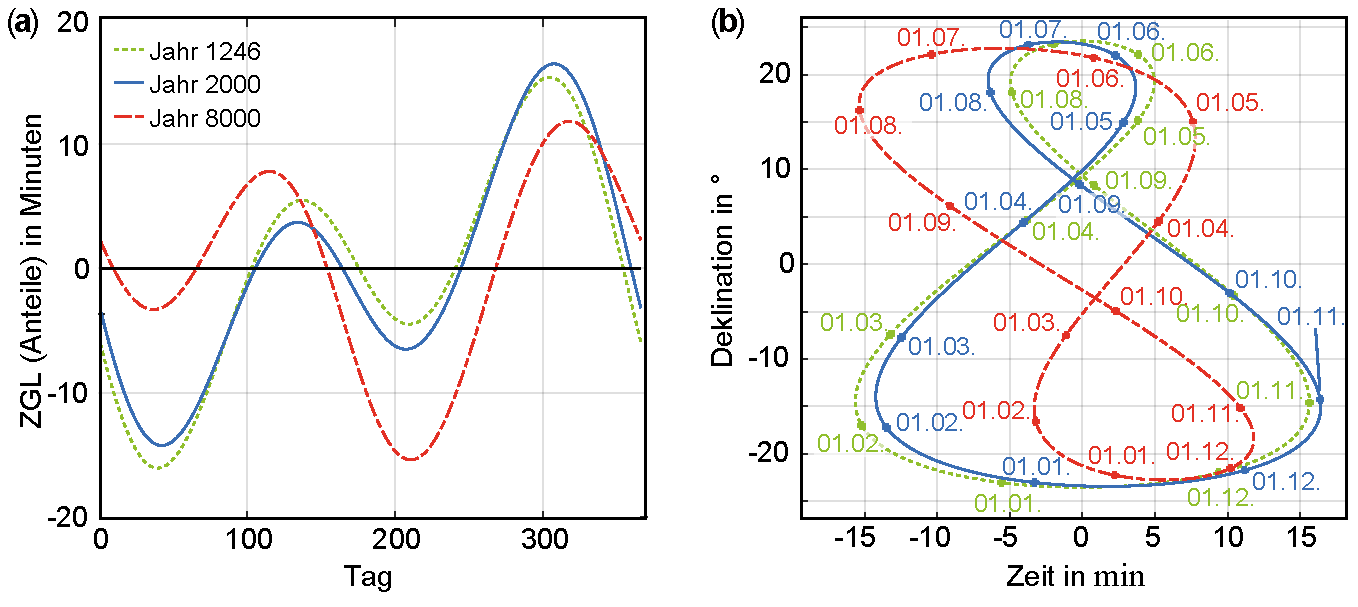
\includegraphics[width=\textwidth]{ZGL_Analemma_long.pdf}%
\caption[Zeitgleichung und Analemma f�r verschiedene Zeiten.]{\fa Zeitgleichung und \fb Analemma f�r die Jahre 1246, 2000 und 8000 u.Z.}%
\label{abb:hm_ZGL_Analemma_long}%ZGLAnnalong
\end{figure}


\subsection{Zeitr�ume von Millionen von Jahren -- Klimaeffekte}\label{kap:hm_ganz_langezeiten}

Wir wollen jetzt unser Modell noch etwas \anf{strapazieren} und auf noch l�ngere Zeiten ausdehnen.
Wir machen dabei starke Vereinfachungen hinsichtlich der Annahmen f�r die zeitlichen Entwicklung der Bahnparameter, f�r die wir einfache Periodizit�ten annehmen.
F�r die Exzentrizit�t haben wir im Mittel $e_m\!=\!0.028$ angenommen.
Dabei gibt es eine Periode von 405\,000 Jahren (Variation der Exzentrizit�t um $\pm 0.012$) und einen Zyklus von 100\,000 Jahren (Variation zwischen $-0.03$ und $+0.02$).
Ebenso nehmen wir f�r die Ekliptikschiefe eine Periodizit�t von 41\,000 Jahren um den Mittelwert $22.8\degree$ an und f�r die Perihelverschiebung einen gleichf�rmigen Zuwachs von $1.7192 \degree$ pro Jahrhundert.
\begin{figure}%
	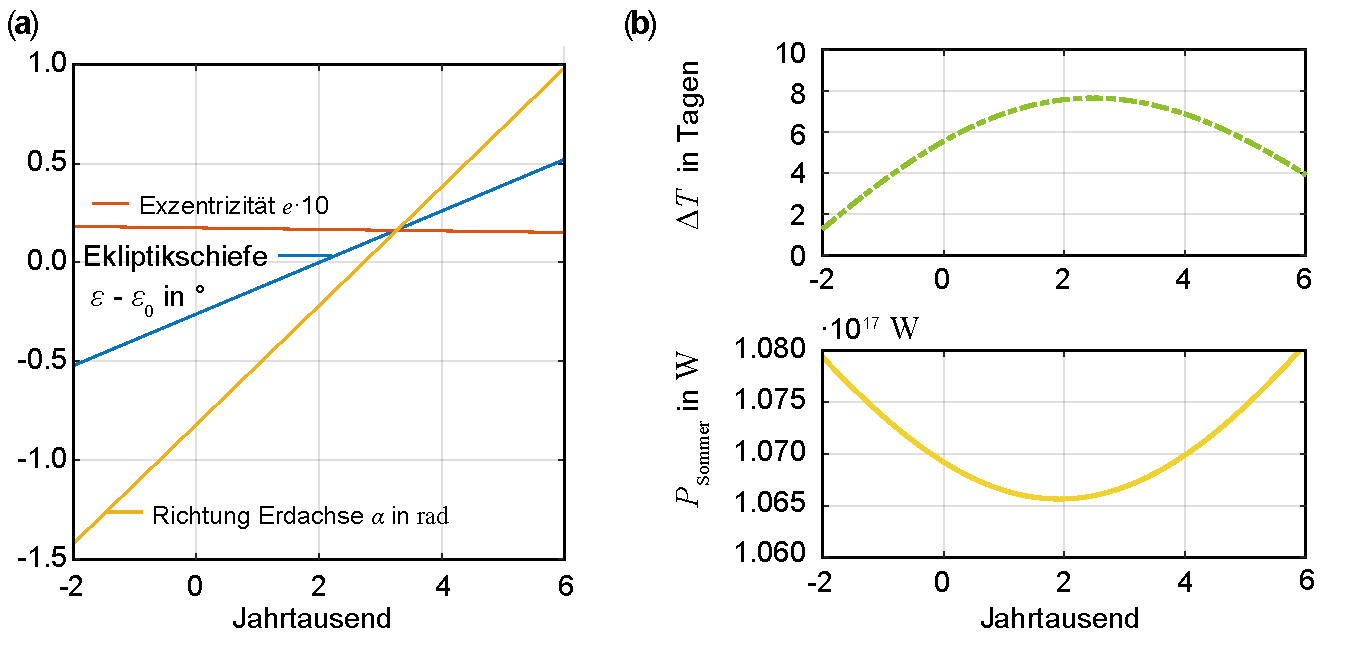
\includegraphics[width=\textwidth]{Erdbahn_im_Jahr_lsg_low.pdf}%
	\caption[Ver�nderung der Bahnparameter der Erde.]{\fa Ver�nderung der Bahnparameter der Erde �ber einen Zeitraum von 8000 Jahren und \fb Variation der Differenz UT-ET sowie der mittleren eingestrahlte Sonnenleistung auf die Nordhalbkugel in demselben Zeitraum.}
	\label{abb:hm_Nordsommer_long}%NordSommer
	\end{figure}

Wir geben hier nur unser Ergebnis der Rechnungen in \figref{hm_Nordsommer_long} an, zum Vergleich siehe auch die Ref. \cite{Rainey2022}.
Wir erkennen deutlich Periodizit�ten beim mittleren Energieeintrag.
Will man die Frage beantworten, ob diese ohne Zweifel vorhandenen (astrosolaren) Effekte einen signifikanten Einflussfaktor auf unser Klima\index{Klimaeffekt} darstellen oder vielleicht sogar dominant f�r die langfristige Entwicklung des Erdklimas mit seinem h�ufigen Wechsel von Warm- und Kaltperioden sind, dann muss man deutlich l�ngere Zeiten betrachten (\ca 1~Mio.~Jahre) und auch detailliertere Rechnungen anstellen.
Beispielsweise muss man die Verteilung von Kontinental- und Wassermassen, unterschiedliche Reflektions-, Speicher- und Abstrahlverhalten ber�cksichtigen und vor allem auch breitengradabh�ngig rechnen und nicht nur �ber die Hemisph�re integrieren.
Auf Grund von solchen (hier nur prinzipiell dargestellten) Berechnungen und deren Vergleich mit empirischen Untersuchungen des Langzeitverhaltens des Klimas ist heute im Allgemeinen anerkannt, dass die in dem \emph{Milankovic}-Zyklus\index{Milankovic-Zyklus}\footnote{Milutin Milankovic (1879--1958) war ein jugoslawischer Bauingenieur, Mathematiker und Geowissenschaftler, der als erster die Berechnung der nach ihm benannten Klima-Zyklen durchf�hrte und damit das Gebiet der der Pal�oklimatologie begr�ndete.} gezeigten periodischen Effekte mit den astronomischen Bahnparametern korrelieren (\figref{hm_Milankovic}) \cite{Milankovic1941}.
Das Bild zeigt die Variation der Erdbahnparameter, die im Vergleich zu unserem Modell deutlich pr�ziser modelliert wurden.
Gleichwohl werden die wesentlichen Effekte auch in unserem Modell sichtbar.
Vor allem periodische Ver�nderungen des solaren Energieeintrags in hohen geographischen Breiten und die Korrelation zu den beobachteten Eiszeiten kann man ableiten.
Nach der Milankovic-Theorie sind die 100\,000 Jahre-Periodizit�ten in den Eiszeiten eben durch die unterschiedliche in den h�heren Breiten im nordischen Sommer einfallende Sonnenenergie verursacht, die wiederum aus den Ver�nderungen in der Erdachsenneigung und der Perihelverschiebung\index{Perihelverschiebung} resultiert.
Allerdings hat die moderne Klimaforschung gezeigt, dass neben diesen langfristig wirkenden Klimafaktoren auch andere nat�rliche Faktoren wie Vulkanismus und die solare Aktivit�t (Sonnenflecken, Protuberanzen) wichtige Rollen spielen.
In den letzten 100--200 Jahren nimmt aber der Einfluss der anthropogenen Faktoren (Waldrodung, Kohlendioxid-Aussto� \cite{Bauer2003, Bauer2005}) signifikant zu.

	\begin{figure}%
	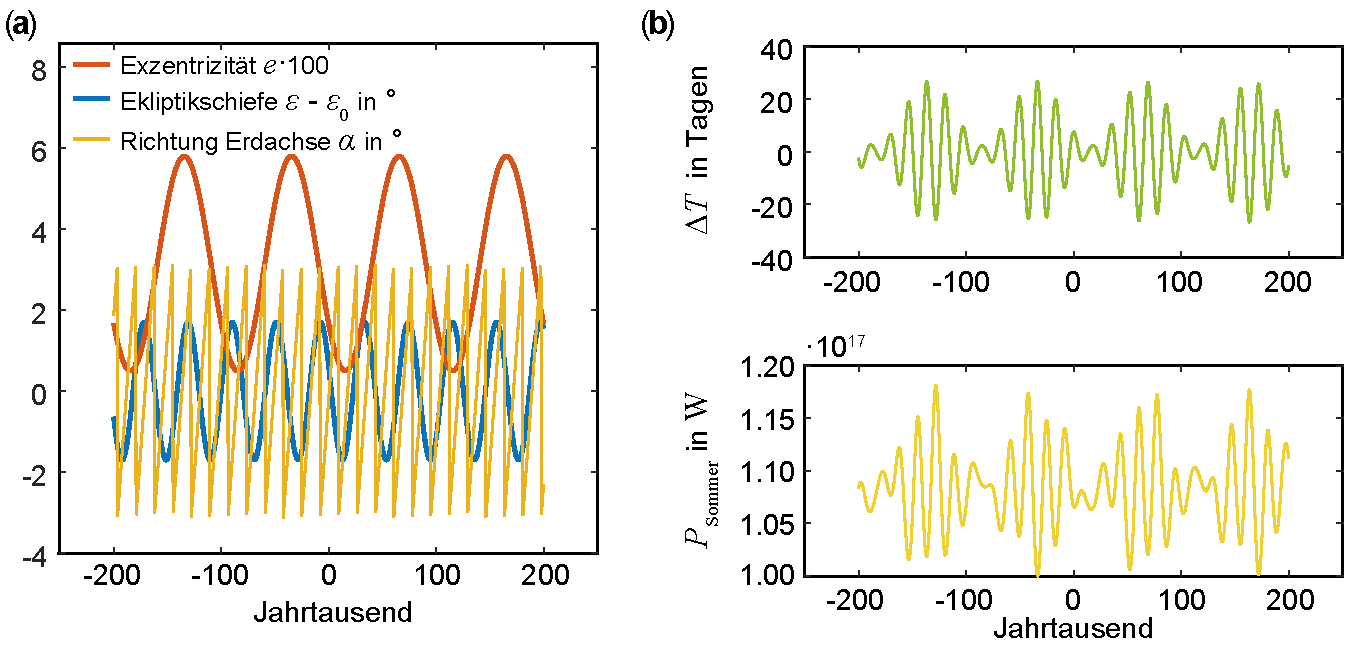
\includegraphics[width=\textwidth]{Nordsommer_long.pdf}%
	\caption[Mittlere eingestrahlte Sonnenleistung auf die Nordhalbkugel f�r sehr lange Zeiten.]{\fa Ver�nderung der Bahnparameter der Erde und \fb Variation der Differenz UT-ET sowie der mittleren eingestrahlten Sonnenleistung auf die Nordhalbkugel w�hrend des Nordsommers f�r sehr lange Zeiten.}%
	\label{abb:hm_Nordsommer_long_long}%NordSommer
	\end{figure}

	\begin{figure}%
	\centering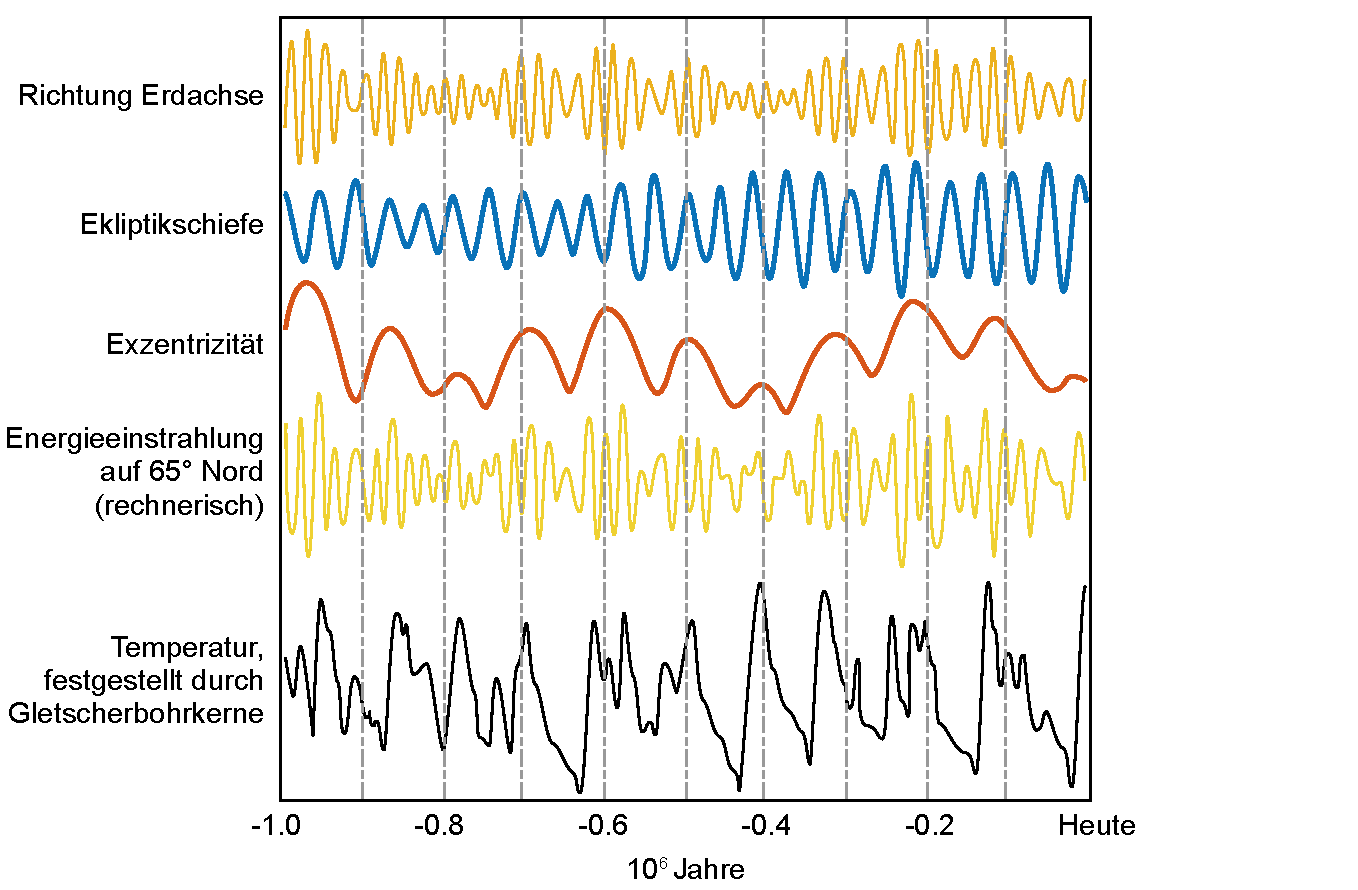
\includegraphics[width=\textwidth]{Milankovic.pdf}%
	\caption[Milankovic-Zyklen f�r einen Zeitraum von 1 Million Jahren.]{Milankovic-Zyklen f�r einen Zeitraum von 1~Mio.~Jahren \cite{Rohde2006}.
        Das Bild ist gestaltet nach einem f�r das Global Warming Art Project frei zug�nglichem Bild von Robert A. Rhode. }
	\label{abb:hm_Milankovic}%Milankovic
	\end{figure}




\clearpage
%%% Anmerkung 2023-11-13 (mk.):
%%% Links auf L�sungen komplett auskommentiert, da extra file bew_uebungenAB.tex
%%% Einfaches �ndern durch  ersetzen \hyperref.. <--> %\hyperref.

%%% Links basieren f�r ein m�gliches e_book auf getrennter pdf-Zieldokumente auf pdf-Hypertags:
%%%        \linklsg\\%\href{FingerUeb2_AB.pdf#prb:hm_trafo_koord}{\textcolor{blue} {$\rightarrow$ zur \probref{hm_trafo_koord}.}}\\
%%% Einfaches �ndern durch  ersetzen %href{FingerUeb1_AB.pdf.. <--> \linklsg\\%\href{FingerUeb1_AB.pdf..
%%%
%%% oder 
%%% f�r das Arbeitsbuch als geschlossenes Zieldokument auf normalen Verweisen (siehe bew_uebungenAB.tex):
%%%        \textcolor{blue} {$\rightarrow$ zur} \probref{hm_trafo_koord}.\\
%%%

\section{�bungen zu \autoref{chap:hm} -- Himmelsmechanik}\label{kap:bm_uebungen}

\medskip
Die �bungen sind mit Schwierigkeitsindikatoren markiert, von einfach ($\ast$) �ber mittel ($\ast \ast$) bis schwierig ($\ast \ast \ast$).
Zusatzaufgaben sind zum Teil mit ($\ast \ast \ast \;!$) markiert und eher als Erweiterung des Theorieteils zu betrachten.
Einige wenige �bungen sind rein analytisch, die gro�e Mehrzahl beinhaltet aber \matlab-Anwendungen. \\

L�sungsbeispiele finden sich in den \onlineZ{} im Arbeitsbuch {\textcolor{blue}{FingerUeb2\_AB.pdf}} und k�nnen �ber den Link \linklsg erreicht werden.\\
Die entsprechenden \mscre finden sich im GitHub unter \githubSN \bzw
in den \onlineZ{} (\MKc).\\


%%%-----------------------------------------------------------------------------------------------------------

\subsection{�bungen zu Raum und Zeit in der Himmelsmechanik}

\medskip

%-----------------------------------------------------------------------------------------------------------

\begin{prob} %�bung1
\einfach{hm_trafo_koord}{Transformation astronomischer Koordinatensysteme} 
Wir wollen uns mit den verschiedenen astronomischen KOS vertraut machen.
\begin{enumerate}
	\item Leiten Sie die Transformationsmatrizen f�r die KOS-Transformationen in Tabelle \ref{tab:hm_Umrechung_KOS} im Tabellenanhang ab und verifizieren Sie die dort angegebenen Formeln. 
	\item Eine sch�ne Anwendung der Transformationsgleichung ist die Navigation in der Seefahrt.
          Zur Bestimmung des L�ngengrades auf See benutzte man folgende Methode: Ein Stern mit bekannten Koordinaten $\alpha_1$, $\delta_1$ steht zu einer bestimmten, bekannten Zeit GMST ($=\theta_0$) �ber einem Punkt der Erde mit den Koordinaten $\lambda\!=\!\theta_0-\alpha$ und $\varphi$ genau im Zenit.
          Sein Stundenwinkel $\tau$ ist dann offensichtlich $0$.
          Alle Orte, f�r die dieser Stern zu einem festen Zeitpunkt $t$ die Zenitdistanz $z$ hat, liegen dann auf einem Kreis mit dem Radius $z_1$ um $\lambda$, $\varphi$.
          Dieser Kreis wird auch Standlinie genannt.
          Bestimmt man also zu einem Zeitpunkt $t$ die Zenitdistanz $z_1\!=\!90\degree-h_1$ eines bekannten Sterns mit den Koordinaten ($\alpha_1$ , $\delta_1$), dann befindet man sich irgendwo auf dieser Standlinie.
          Jetzt sucht man einen zweiten Stern mit ($\alpha_2$, $\delta_2$) und bestimmt wieder die Zenitdistanz $z_2$.
          Dann erh�lt man eine weitere Standlinie, die die erste an zwei Punkten schneidet.
          Einer dieser Schnittpunkte ist der gesuchte Ort.
          Um zu entscheiden, welcher von beiden Punkten der richtige ist, benutzt man eine iterative Methode.
          Ausgangspunkt daf�r ist meist die letzte bekannte Position.
          Man vollziehe diese Bestimmung des L�ngengrades mittels der in Tabelle \ref{tab:hm_astro_KOS} und Tabelle \ref{tab:hm_Umrechung_KOS} angegebenen Beziehung nach.
\end{enumerate}

\medskip 
%\hyperref[lsg:adyn_canonball]{\textcolor{blue} {$\rightarrow$ L�sungsvorschlag}}\\
\linklsg\\%\href{FingerUeb2_AB.pdf#lsg:adyn_canonball}{\textcolor{blue} {$\rightarrow$ L�sungsteil}}.\\
\noindent\rule[1ex]{\textwidth}{0.5pt}
\end{prob}

%-----------------------------------------------------------------------------------------------------------

\newpage
\begin{prob} %�bung2
\mittel{hm_erdrotation}{Verlangsamung der Erdrotation}
Berechnen Sie die Verschiebung der Zeitmarken der Sonnenfinsternisse durch die Verlangsamung der Erdrotation.
Als N�herungsformel kann man f�r die Abnahme in Sekunden folgende Beziehung annehmen:
\begin{equation}
\Delta T_\text{rot} = \frac{0.9}{10^5 \, a_\text{trop}} \: n^2_\text{Tage} ~.\label{eq:hm_ueb_verl_erdrot}
\end{equation}
Hier sind $n_\text{Tage}$ die Zahl der vergangenen Tage und $a_\text{trop}$ die Dauer eines tropischen Jahres in Tagen.
Erkl�ren Sie damit, dass man mit einem heutigen Astroprogramm die Sonnenfinsternis in Babylon vom 15.04.136 v. Chr. ca. $40$\textdegree\ westlich von Babylon berechnet, obwohl die babylonischen Astronomen diese sehr genau in Babylon registriert hatten.
Dem interessierten Leser sei die Literatur \cite{Stephenson2016,Steele1997} empfohlen und ebenso die \href{https://eclipse.gsfc.nasa.gov/SEsearch/SEsearchmap.php?Ecl=-1350415}{NASA Eclipse Web Site}.

\medskip 
%\hyperref[lsg:hm_erdrotation]{\textcolor{blue} {$\rightarrow$ L�sungsvorschlag}}\\
\linklsg\\%\href{FingerUeb2_AB.pdf#lsg:hm_erdrotation}{\textcolor{blue} {$\rightarrow$ L�sungsteil}}.\\
\noindent\rule[1ex]{\textwidth}{0.5pt}
\end{prob}

%-----------------------------------------------------------------------------------------------------------

\begin{prob} %�bung3
\einfach{hm_sideric_period_mars}{Siderische Umlaufzeit des Mars}
Berechnen Sie die siderische Umlaufzeit des Mars aus den beobachteten Zeitabst�nden zwischen zwei aufeinanderfolgenden Oppositionen des Planeten.

\medskip 
%\hyperref[lsg:hm_sideric_period_mars]{\textcolor{blue} {$\rightarrow$ L�sungsvorschlag}}\\
\linklsg\\%\href{FingerUeb2_AB.pdf#lsg:hm_sideric_period_mars}{\textcolor{blue} {$\rightarrow$ L�sungsteil}}.\\
\noindent\rule[1ex]{\textwidth}{0.5pt} 
\end{prob}

%%%-----------------------------------------------------------------------------------------------------------
\newpage
\subsection{�bungen zur Kepler-Gleichung}

\medskip

%-----------------------------------------------------------------------------------------------------------

\begin{prob} %�bung4
\einfach{hm_laplace}{Laplace-Integral}
Leiten Sie aus \eqref{eq:hm_zk-pl} das Laplace-Integral nach \eqref{eq:hm_laplace_int} ab.
Zeigen Sie au�erdem, dass f�r den Laplacevektor $\vec{e}$ aus \eqref{eq:hm_laplace_int} die Beziehungen $\vec{L}\cdot\vec{e}\!=\!0$ und
\begin{align*}
\mu_\text{G}^2\,\lk\abs{\vec{e}}^2 - 1\rk &= 2H \abs{\vec{L}}^2 ~~\text{bzw.} \\
e^2 &= \frac{2HL^2}{\mu_\text{G}^2} + 1 
\end{align*}
gem�� \eqref{eq:hm_relations1} gelten.

\medskip 
%\hyperref[lsg:hm_laplace]{\textcolor{blue} {$\rightarrow$ L�sungsvorschlag}}\\
\linklsg\\%\href{FingerUeb2_AB.pdf#lsg:hm_laplace}{\textcolor{blue} {$\rightarrow$ L�sungsteil}}.\\

\noindent\rule[1ex]{\textwidth}{0.5pt}
\end{prob}

%-----------------------------------------------------------------------------------------------------------

\begin{prob} %�bung5
\einfach{hm_wahre_anomalie}{Wahre Anomalie}
Leiten Sie die Beziehung \eqref{eq:hm_nu(t)_alternativ} her:
\begin{equation*}
\tan\lk\frac{\upsilon}{2}\rk = \sqrt{\frac{1+e}{1-e}} \tan\lk\frac{E}{2}\rk ~~.
\end{equation*}

\medskip 
%\hyperref[lsg:hm_wahre_anomalie]{\textcolor{blue} {$\rightarrow$ L�sungsvorschlag}}\\
\linklsg\\%\href{FingerUeb2_AB.pdf#lsg:hm_wahre_anomalie}{\textcolor{blue} {$\rightarrow$ L�sungsteil}}.\\
\noindent\rule[1ex]{\textwidth}{0.5pt} 
\end{prob}

%-----------------------------------------------------------------------------------------------------------

\begin{prob} %�bung6
\mittel{hm_bwglg_hyp_parab}{Bewegungsgleichungen f�r Hyperbel und Parabel}
Leiten Sie die zur Kepler-Gleichung \eqref{eq:hm_keplerglg} �quivalente Beziehung f�r Hyperbel- und Parabelbahnen ab.
Was k�nnen Sie zur L�sungsproblematik f�r beide F�lle sagen?
Geben Sie eine geschlossene L�sung f�r den Fall der Parabel an.

\medskip 
%\hyperref[lsg:hm_bwglg_hyp_parab]{\textcolor{blue} {$\rightarrow$ L�sungsvorschlag}}\\
\linklsg\\%\href{FingerUeb2_AB.pdf#lsg:hm_bwglg_hyp_parab}{\textcolor{blue} {$\rightarrow$ L�sungsteil}}.\\
\noindent\rule[1ex]{\textwidth}{0.5pt}
\end{prob}

%-----------------------------------------------------------------------------------------------------------

\begin{prob} %�bung7
\einfach{hm_iteration}{Iteration}
F�hren Sie das in \kapitel{iteration_kepler} beschriebene Iterationsverfahren numerisch f�r verschiedene Exzentrizit�ten $e\!=\!0.1,\,0.2,\,\ldots ,\,0.9$ und $0.999$ durch.
W�hlen Sie als Anfangswert neben $M$ auch andere Werte.
Vergleichen Sie die Ergebnisse jeweils mit den Ergebnissen zweier anderer N�herungsverfahren (Regula falsi und Newton-Raphson).

\medskip 
%\hyperref[lsg:hm_iteration]{\textcolor{blue} {$\rightarrow$ L�sungsvorschlag}}\\
\linklsg\\%\href{FingerUeb2_AB.pdf#lsg:hm_iteration}{\textcolor{blue} {$\rightarrow$ L�sungsteil}}.\\
\noindent\rule[1ex]{\textwidth}{0.5pt}
\end{prob}

%-----------------------------------------------------------------------------------------------------------

\begin{prob} %�bung8
\mittel{hm_bessel}{Bessel-Reihe}
F�hren Sie die Reihenentwicklung \eqref{eq:hm_lsg_kepler_reihe} f�r die Bessel-L�sung einmal selbst bis zur vierten Ordnung in $e$ f�r verschiedene Exzentrizit�ten $e\!=\!0.1,\,0.2,\,\ldots ,\,0.9$ und $0.999$ durch.
Vergleichen Sie das Ergebnis mit der numerischen Berechnung nach \probref{hm_iteration}. 

\medskip 
%\hyperref[lsg:hm_bessel]{\textcolor{blue} {$\rightarrow$ L�sungsvorschlag}}\\
\linklsg\\%\href{FingerUeb2_AB.pdf#lsg:hm_bessel}{\textcolor{blue} {$\rightarrow$ L�sungsteil}}.\\
\noindent\rule[1ex]{\textwidth}{0.5pt}
\end{prob}

%-----------------------------------------------------------------------------------------------------------

\begin{prob} %�bung9
\schwierig{hm_alternative_MPG}{Alternative Herleitung der Mittelpunktsgleichung}
Leiten Sie die Mittelpunktsgleichung auf einem alternativen Weg her.
Starten Sie dabei von \eqref{eq:hm_nu(t)_alternativ} und benutzen Sie vorteilhafterweise komplexe Winkelfunktionen sowie die Bessel-Reihe \eqref{eq:hm_lsg_kepler_reihe}. 

\medskip 
%\hyperref[lsg:hm_alternative_MPG]{\textcolor{blue} {$\rightarrow$ L�sungsvorschlag}}\\
\linklsg\\%\href{FingerUeb2_AB.pdf#lsg:hm_alternative_MPG}{\textcolor{blue} {$\rightarrow$ L�sungsteil}}.\\
\noindent\rule[1ex]{\textwidth}{0.5pt}
\end{prob}

%%%-----------------------------------------------------------------------------------------------------------
\newpage
\subsection{�bungen zur Bewegung der Erde in der Ekliptik und zu Himmelsbeobachtungen von der Erde}

\medskip

%-----------------------------------------------------------------------------------------------------------

\begin{prob} %�bung10
\mittel{hm_erdbahn_im_jahr}{Die Erdbahn im Laufe eines Jahres}
Berechnen Sie die Aphel- und Perihel-Distanz der Erde, den �ber ein Jahr zeit- und raumgemittelten Abstand der Erde von der Sonne, die Dauer der Jahreszeiten und den Energieeintrag der Sonne auf die Nordhemisph�re jeweils f�r das Sommer- und Winterhalbjahr.
Was k�nnen Sie daraus zum Einfluss auf m�gliche Klimaver�nderungen sagen?

\medskip 
%\hyperref[lsg:hm_erdbahn_im_jahr]{\textcolor{blue} {$\rightarrow$ L�sungsvorschlag}}\\
\linklsg\\%\href{FingerUeb2_AB.pdf#lsg:hm_erdbahn_im_jahr}{\textcolor{blue} {$\rightarrow$ L�sungsteil}}.\\
\noindent\rule[1ex]{\textwidth}{0.5pt}
\end{prob}

%-----------------------------------------------------------------------------------------------------------

\begin{prob} %�bung11
\schwierig{hm_refrak_optik}{Refraktion -- ein Ausflug in die Optik}
F�r die Berechnung der Refraktion gibt es zwei einfache Schichten-Modelle: das planparallele Modell und das Kugelschalenmodell (\figref{hm_refr_kugelschale}).
Berechnen Sie die Refraktion $R(z)$ f�r beide Modelle und erl�utern Sie, f�r welches der beiden Modelle Sie sich bei der Beobachtung von Sonnenaufg�ngen entscheiden w�rden.
In welcher Situation ist das jeweils andere Modell vorteilhaft?
K�nnen Sie mit einem dieser Modelle die Beziehung \eqref{eq:hm_tau_zgl} erkl�ren? \\
Hinweise: Mit $z_\infty$ wird die wahre Zenitdistanz bezeichnet.
Es gilt dann $z_\infty\!=\!90\degree-h$.
Analog gilt f�r die scheinbare Zenitdistanz $z_1\!=\!z'\!=\!90\degree-h'$.
Mit $\D R$ wird die differentielle Refraktion beschrieben.
F�r die Brechzahl gilt:
\begin{equation*}
\frac{n^2-1}{n^2+2}\!=\!\rho\!=\!\frac{\bar{\mu}_\text{molek}p}{TR_0} \; .
\end{equation*}
Hierin ist $\bar{\mu}_\text{molek}$ das mittlere Molekulargewicht, $R_0$ die universelle Gaskonstante, $T$ die Temperatur und $p$ der Druck.
\begin{figure}%
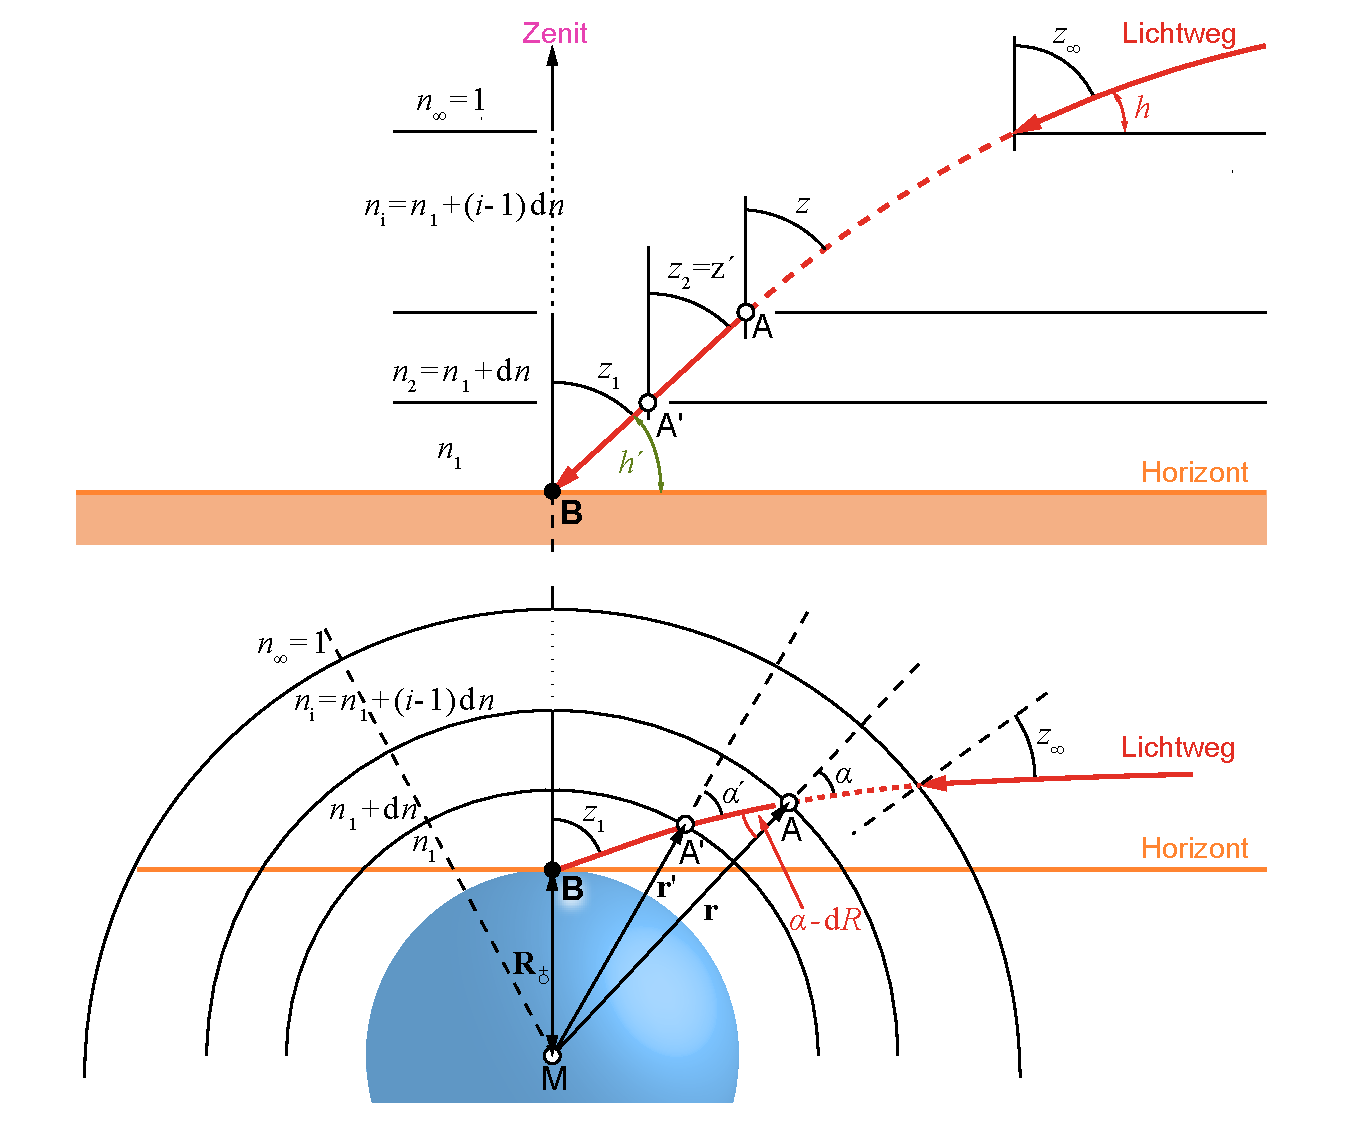
\includegraphics[width=\textwidth]{Refraktion0102.pdf}%
\caption[Planparalleles und Kugelschalen-Schichtenmodell.]{Planparalleles und Kugelschalen-Schichtenmodell zur Berechnung der Refraktion.
F�r die Winkel im $\bigtriangleup\mathrm{A}'\mathrm{MA}$ gilt: $\angle\mathrm{MA}'\mathrm{A}=180\degree-\alpha'$ und $\angle\mathrm{A}'\mathrm{MA}=\alpha-\D R$.}%
\label{abb:hm_refr_kugelschale}%
\end{figure}

\medskip 
%\hyperref[lsg:hm_refrak_optik]{\textcolor{blue} {$\rightarrow$ L�sungsvorschlag}}\\
\linklsg\\%\href{FingerUeb2_AB.pdf#lsg:hm_refrak_optik}{\textcolor{blue} {$\rightarrow$ L�sungsteil}}.\\
\noindent\rule[1ex]{\textwidth}{0.5pt}
\end{prob}

%-----------------------------------------------------------------------------------------------------------

\begin{prob} %�bung12
\einfach{hm_abflachung_sonne}{Abflachung der Sonne beim Untergang}
Berechnen Sie mit Hilfe von \eqref{eq:hm_tau_zgl} die Abflachung der Sonne, wenn der untere Rand der Sonne gerade die scheinbare H�he $h$ hat und der wahre Winkeldurchmesser der Sonne genau $32'$ betr�gt. 

\medskip 
%\hyperref[lsg:hm_abflachung_sonne]{\textcolor{blue} {$\rightarrow$ L�sungsvorschlag}}\\
\linklsg\\%\href{FingerUeb2_AB.pdf#lsg:hm_abflachung_sonne}{\textcolor{blue} {$\rightarrow$ L�sungsteil}}.\\
\noindent\rule[1ex]{\textwidth}{0.5pt}
\end{prob}

%-----------------------------------------------------------------------------------------------------------

\begin{prob} %�bung13
\einfach{hm_tageslauf_sonne}{Tageslauf der Sonne}
Berechnen Sie den Tageslauf der Sonne mit Ber�cksichtigung der Refraktion $R$ und einer �ber den Tag ver�nderlichen Deklination $\delta$.
Tragen Sie die Abweichung zum berechneten Verlauf bei Benutzung von \eqref{eq:hm_delta_von_T_hash} f�r eine w�hrend des Tages konstant gehaltene Deklination auf.
Vernachl�ssigen Sie f�r die N�herung die Refraktion.
Berechnen Sie den Tageslauf f�r verschiedene geographische Breiten und die �quinoktien bzw. Sonnenwenden.

\medskip 
%\hyperref[lsg:hm_tageslauf_sonne]{\textcolor{blue} {$\rightarrow$ L�sungsvorschlag}}\\
\linklsg\\%\href{FingerUeb2_AB.pdf#lsg:hm_tageslauf_sonne}{\textcolor{blue} {$\rightarrow$ L�sungsteil}}.\\
\noindent\rule[1ex]{\textwidth}{0.5pt}
\end{prob}

%-----------------------------------------------------------------------------------------------------------

\begin{prob} %�bung14
\einfach{hm_sonnenaufg_nyc}{Sonnenaufgang NYC}
Berechnen Sie, um wieviel fr�her ein Beobachter auf dem One World Trade Center (H�he auf dem Dach: $531\:$m) den Sonnenaufgang zur Sommersonnenwende sieht als ein Beobachter am Fu�e der Freiheitsstatue.
Ber�cksichtigen Sie dabei die Refraktion!

\medskip 
%\hyperref[lsg:hm_sonnenaufg_nyc]{\textcolor{blue} {$\rightarrow$ L�sungsvorschlag}}\\
\linklsg\\%\href{FingerUeb2_AB.pdf#lsg:hm_sonnenaufg_nyc}{\textcolor{blue} {$\rightarrow$ L�sungsteil}}.\\
\noindent\rule[1ex]{\textwidth}{0.5pt}
\end{prob}

%-----------------------------------------------------------------------------------------------------------

\begin{prob} %�bung15
\mittel{hm_analytic_sunrise}{Analytische Formel f�r Sonnenauf- und Sonnenuntergang}
Leiten Sie eine handhabbare analytische Formel f�r den Sonnenaufgang her.
Berechnen Sie mit dieser Formel auch eine N�herung f�r die in \figref{hm_Sonnenauf_untergang} dargestellte Verschiebung zwischen dem Tag der Wintersonnenwende und dem k�rzesten Tag bzw. dem Tag mit dem sp�testen Sonnenaufgang (ohne Ber�cksichtigung von Refraktion).\footnote{Wir folgen dabei der Vorgehensweise in \cite{Reinsch2003}.}

\medskip 
%\hyperref[lsg:hm_analytic_sunrise]{\textcolor{blue} {$\rightarrow$ L�sungsvorschlag}}\\
\linklsg\\%\href{FingerUeb2_AB.pdf#lsg:hm_analytic_sunrise}{\textcolor{blue} {$\rightarrow$ L�sungsteil}}.\\
\noindent\rule[1ex]{\textwidth}{0.5pt}
\end{prob}

%-----------------------------------------------------------------------------------------------------------

\begin{prob} %�bung16
\einfach{hm_VertikalAnalemmaSonnenuhr}{Konstruktion von Sonnenuhren}{Konstruktion einer vertikalen und einer analemmatischen Sonnenuhr.}
Berechnen Sie das Ziffernblatt einer Vertikal-Sonnenuhr, die an einer Hauswand angebracht ist, die unter einem beliebigen Winkel $\alpha$ zur Ost-West-Richtung steht (\figref{hm_sundial05}).
Berechnen Sie ebenfalls das Ziffernblatt einer analemmatischen Sonnenuhr f�r die Stadt G�rlitz.

\begin{figure}%
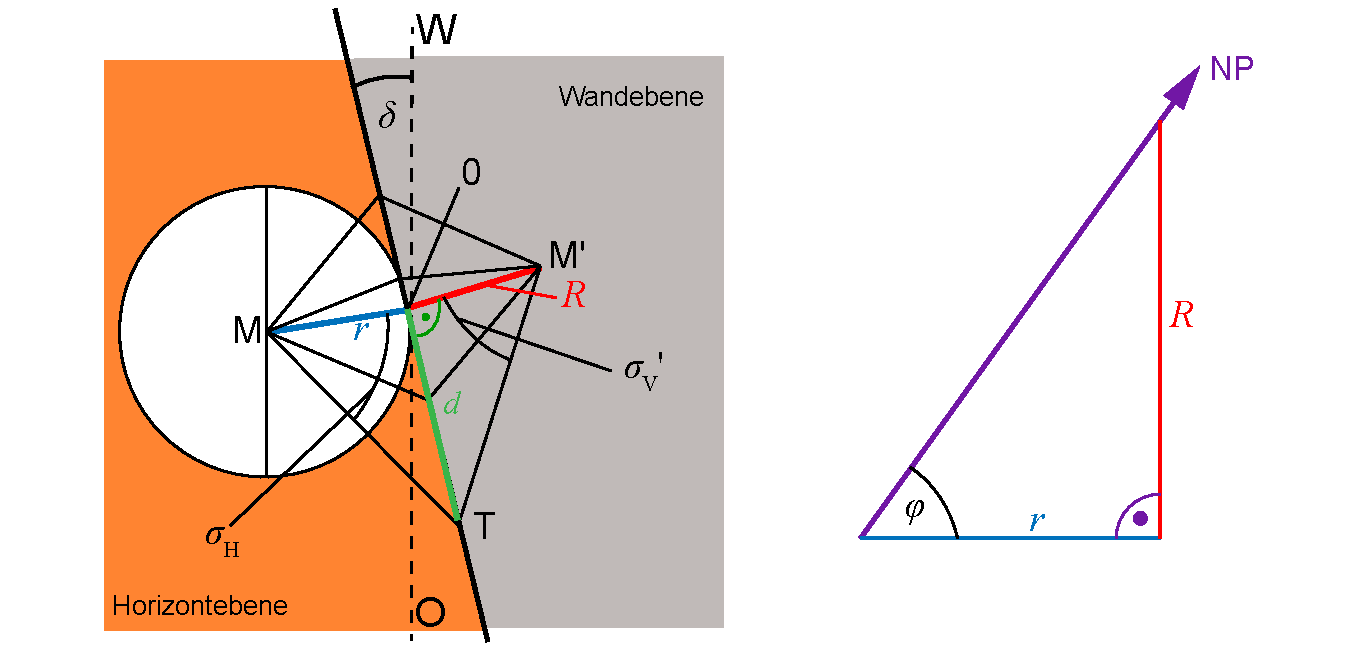
\includegraphics[width=\textwidth]{Sonnenuhr05.pdf}%
\caption[Prinzip der Vertikal-Sonnenuhr.]{Prinzip der Vertikal-Sonnenuhr bei einer beliebigen Ausrichtung der Wand.}%
\label{abb:hm_sundial05}%
\end{figure}


\medskip 
%\hyperref[lsg:hm_VertikalAnalemmaSonnenuhr]{\textcolor{blue} {$\rightarrow$ L�sungsvorschlag}}\\
\linklsg\\%\href{FingerUeb2_AB.pdf#lsg:hm_VertikalAnalemmaSonnenuhr}{\textcolor{blue} {$\rightarrow$ L�sungsteil}}.\\
\noindent\rule[1ex]{\textwidth}{0.5pt}
\end{prob}

%-----------------------------------------------------------------------------------------------------------

\begin{prob} %�bung17
\mittel{hm_opposition_mars}{Mars-Oppositionen von 2000 bis 2040}
Berechnen Sie die Mars-Oppositionen f�r den Zeitraum 2000--2040 und stellen Sie diese f�r den Zeitraum 2002--2020 in einem heliozentrischen Diagramm der Mars- und Erdbahn dar.
Berechnen Sie auch den jeweils kleinsten Abstand des Mars zur Erde und unter welchem H�henwinkel er in Europa zu beobachten war.
Wann hatte man die besten Chancen, Details der Marsoberfl�che zu sehen?
Geben Sie jeweils den Winkeldurchmesser des Mars an, unter dem der Planet zu sehen war.
Wann ist Ihrer Meinung nach die n�chste tolle Beobachtungsgelegenheit? 

\medskip 
%\hyperref[lsg:hm_opposition_mars]{\textcolor{blue} {$\rightarrow$ L�sungsvorschlag}}\\
\linklsg\\%\href{FingerUeb2_AB.pdf#lsg:hm_opposition_mars}{\textcolor{blue} {$\rightarrow$ L�sungsteil}}.\\
\noindent\rule[1ex]{\textwidth}{0.5pt}
\end{prob}

%-----------------------------------------------------------------------------------------------------------

\begin{prob} %�bung18
\schwierig{hm_venus_2004_2012}{Venustransit-Beobachtungen 2004 und 2012} 
Eines der am seltensten von der Erde aus zu beobachtenden Himmelsph�nomene ist der Transit der Venus vor der Sonne.
\begin{enumerate}
	\item Leiten Sie die Beziehung \eqref{eq:hm_Venus_AE_Messung} her und berechnen Sie den effektiven Abstand $d_\text{eff}$ zwischen Troms� (N) und Canberra (AUS) f�r den Venustransit am 06.06.2012 um 03:12 UT.
	\item Leiten Sie die Formel f�r die Kontaktzeitmethode her und berechnen Sie die Abh�ngigkeit des Ergebnisses von der Genauigkeit der Bestimmung der Transitzeiten.
          Beginnen Sie zun�chst mit der vereinfachenden Annahme von konzentrischen und koplanaren Kreisbahnen f�r Venus und Erde.
          Nutzen Sie die erhaltenen Beziehungen f�r die Auswertung der Beobachtungsdaten vom 06.06.2004 in Oberkochen ($\phi = 48.78\degree , \lambda= 10.1\degree$).
          Berechnen Sie den effektiven Abstand $d_\text{eff}$ und daraus die Astronomische Einheit.
          Diskutieren Sie die erreichte Genauigkeit.
          Transitbeginn wurde zu 07:16 MESZ $\pm 1$ min und Transitende zu 13:18 MESZ $\pm 1$ min festgestellt.
          Die relative Sehnenl�nge konnte zu 0.775 bestimmt werden.
	\item Verbessern Sie das Modell, in dem Sie sowohl die Elliptizit�t der Bahnen, als auch die Neigung der Venusbahn gegen die Ekliptik und die topozentrischen Koordinaten des Beobachters ber�cksichtigen.
\end{enumerate}

\medskip 
%\hyperref[lsg:hm_venus_2004_2012]{\textcolor{blue} {$\rightarrow$ L�sungsvorschlag}}\\
\linklsg\\%\href{FingerUeb2_AB.pdf#lsg:hm_venus_2004_2012}{\textcolor{blue} {$\rightarrow$ L�sungsteil}}.\\
\noindent\rule[1ex]{\textwidth}{0.5pt}
\end{prob}

%-----------------------------------------------------------------------------------------------------------

\begin{prob} %�bung19
\schwierig{hm_jupiterbedeckung_venus}{Jupiterbedeckung durch die Venus am 22.11.2065}
Berechnen Sie f�r den 22.11.2065 von 0:00 bis 24:00 UT die geozentrisch-�quatorialen Koordinaten von Jupiter und Venus.
Benutzen Sie zum einen die einfache Keplerl�sung und zum anderen die Reihenentwicklung aus der St�rungsrechnung.
Vergleichen Sie die beiden Ergebnisse (Beachten Sie dabei den Unterschied von UT und ET!).\\
In welchen Regionen der Erde kann man eine Bedeckung des Jupiters beobachten?
Berechnen Sie dazu die Winkeldurchmesser der beiden Planeten von der Erde aus ($R_{\venus}\!=\!6051\:\text{km}$, $R_{\jupiter}\!=\!69911\:\text{km}$).
M�ssen die Lichtlaufzeiten ber�cksichtigt werden (siehe \kapitel{kometen})?

\medskip 
%\hyperref[lsg:hm_jupiterbedeckung_venus]{\textcolor{blue} {$\rightarrow$ L�sungsvorschlag}}\\
\linklsg\\%\href{FingerUeb2_AB.pdf#lsg:hm_jupiterbedeckung_venus}{\textcolor{blue} {$\rightarrow$ L�sungsteil}}.\\
\noindent\rule[1ex]{\textwidth}{0.5pt}
\end{prob}

\newpage
%%%-----------------------------------------------------------------------------------------------------------

\subsection{�bungen zu Himmelsbeobachtungen von anderen Himmelsk�rpern aus}

\medskip

%-----------------------------------------------------------------------------------------------------------

\begin{prob} %�bung20
\einfach{hm_erdaufgang_von_mond}{Kann man einen Erdaufgang vom Mond aus sehen?}
Gibt es f�r einen Astronauten auf dem Mond Erdauf- und Erdunterg�nge?
Wenn ja, unter welchen Bedingungen?
Hinweis: Ber�cksichtigen Sie, dass die gebundene Rotation des Mondes wegen der elliptischen Bahn des Mondes nicht ganz vollst�ndig ist (sogenannte Libration).
H�tte die Apollo 11 Mannschaft die Chance gehabt, Aufg�nge der Erde von der Mondoberfl�che aus zu sehen? 

\medskip 
%\hyperref[lsg:hm_erdaufgang_von_mond]{\textcolor{blue} {$\rightarrow$ L�sungsvorschlag}}\\
\linklsg\\%\href{FingerUeb2_AB.pdf#lsg:hm_erdaufgang_von_mond}{\textcolor{blue} {$\rightarrow$ L�sungsteil}}.\\
\noindent\rule[1ex]{\textwidth}{0.5pt}
\end{prob}

%-----------------------------------------------------------------------------------------------------------

\begin{prob} %�bung21
\mittel{hm_erdaufgang_von_apollo}{Earth Rise von Apollo 8}
Erkl�ren Sie das Zustandekommen des ber�hmten Bildes \anf{Earth Rise} (aufgenommen am 24.12.1968 um ca: 16:38 UT bzw. 75:47 h Bordzeit von Apollo 8).
Berechnen Sie mit den Ihnen in den \mscren zur Verf�gung stehenden Routinen die Konstellation von Mond, Erde, Sonne und Raumschiff und stellen Sie diese graphisch dar.
Finden Sie die Bahndaten von Apollo 8 aus der Literatur.
Benutzen Sie daf�r die Webseite der NASA \href{https://nasa.gov/history} und \href{https://www.nasa.gov/wp-content/uploads/static/history/alsj/a11/a11fltpln_final_reformat.pdf}.
Ebenfalls sehr instruktiv und hilfreich ist das Video der NASA: \href{https://www.youtube.com/watch?v=dE-vOscpiNc}{https://www.youtube.com/watch?v=dE-vOscpiNc}.
\begin{figure}%
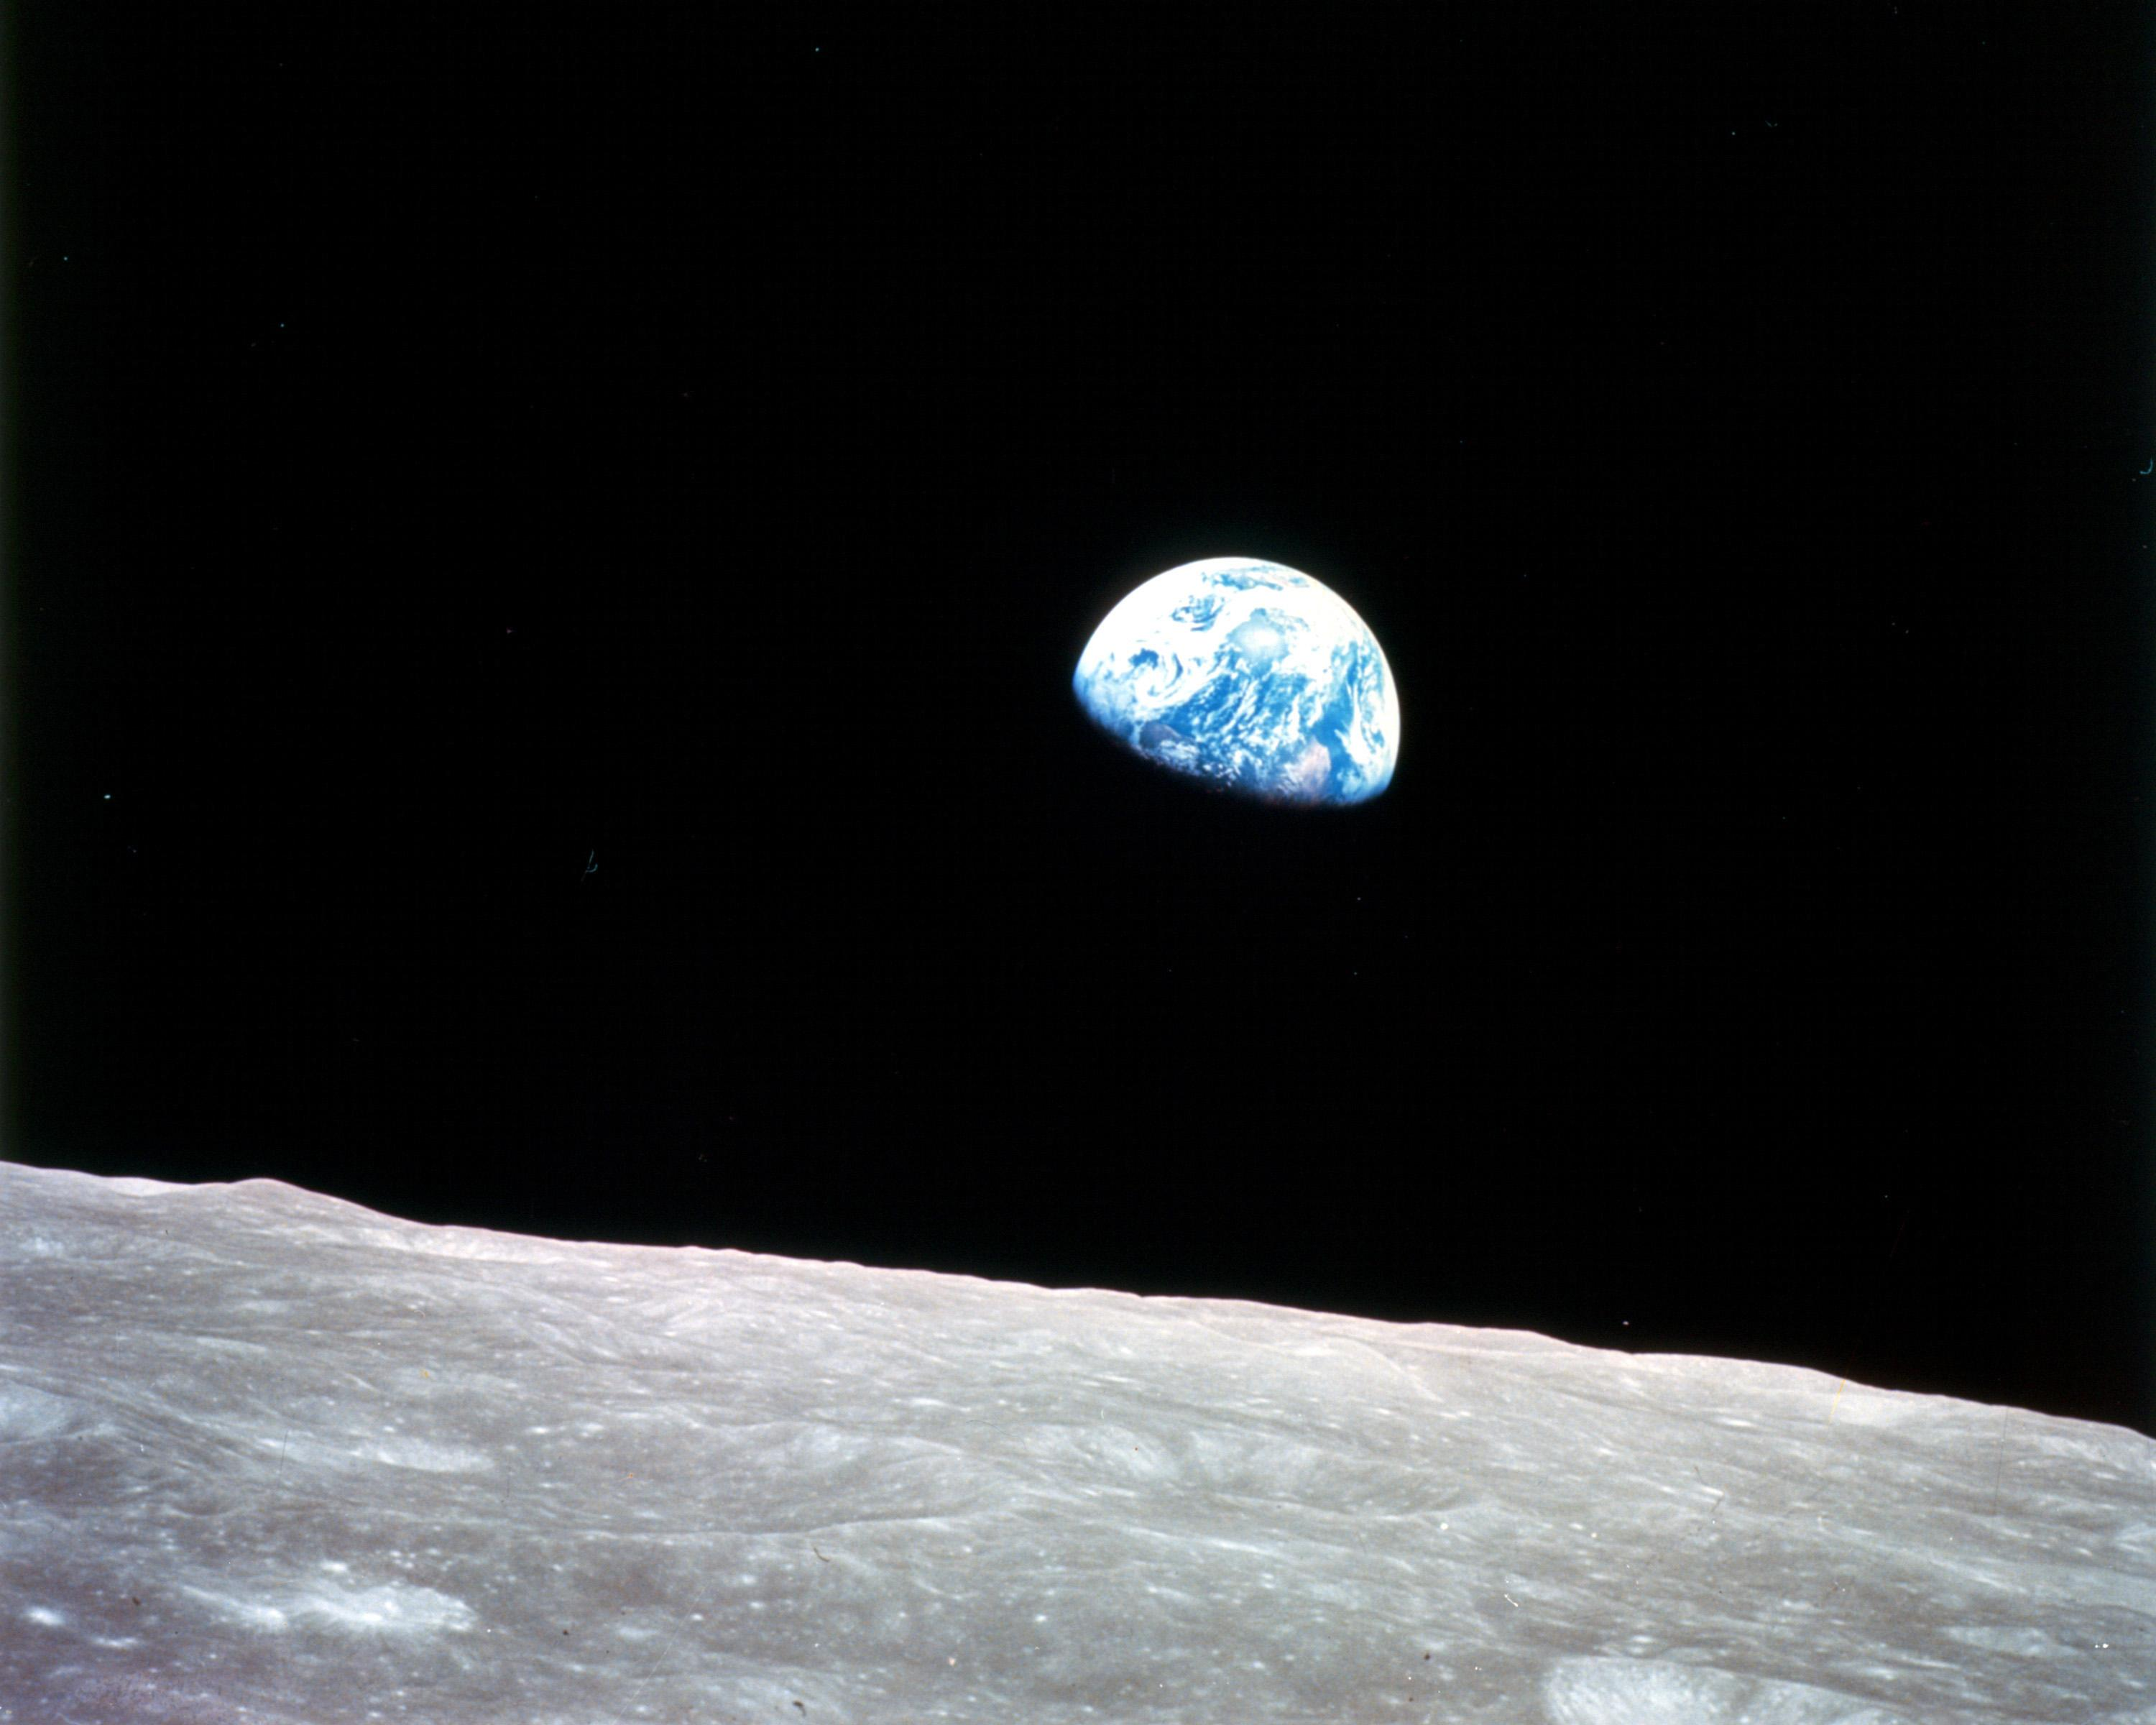
\includegraphics[width=0.6\textwidth]{Earth_Rise_Nasa.jpg} \label {abb:hm_earthrise}
\caption[Earth Rise aufgenommen am 24.12.1968 von Apollo 8.]{Earth Rise aufgenommen am 24.12.1968 von Apollo 8. (Copyright NASA).}% 
\end{figure}

\medskip 
%\hyperref[lsg:hm_erdaufgang_von_apollo]{\textcolor{blue} {$\rightarrow$ L�sungsvorschlag}}\\
\linklsg\\%\href{FingerUeb2_AB.pdf#lsg:hm_erdaufgang_von_apollo}{\textcolor{blue} {$\rightarrow$ L�sungsteil}}.\\
\noindent\rule[1ex]{\textwidth}{0.5pt}
\end{prob}


%-----------------------------------------------------------------------------------------------------------

\begin{prob} %�bung22
\schwierig{hm_Analemma_Mars}{Zeitgleichung und Analemmas auf anderen Planeten}
Die NASA (NASA/JPL/Cornell/ASU/TAMU) ver�ffentlichte das vom Mars-Rover Opportunity aufgenommene Analemma (\figref{hm_Mars_Analemma}).
Dieser fotografierte ein Marsjahr lang  jeden 3. Sol (Marstag) um 11:02 mittlere Ortszeit ein Bild mit der Sonne (in Richtung Zenit).
Daraus resultiert dieses Marsanalemma.
In UTC-Zeit entsprach das dem Zeitraum zwischen dem 16. Juli 2006 und dem 2. Juni 2008. 

\begin{figure}%
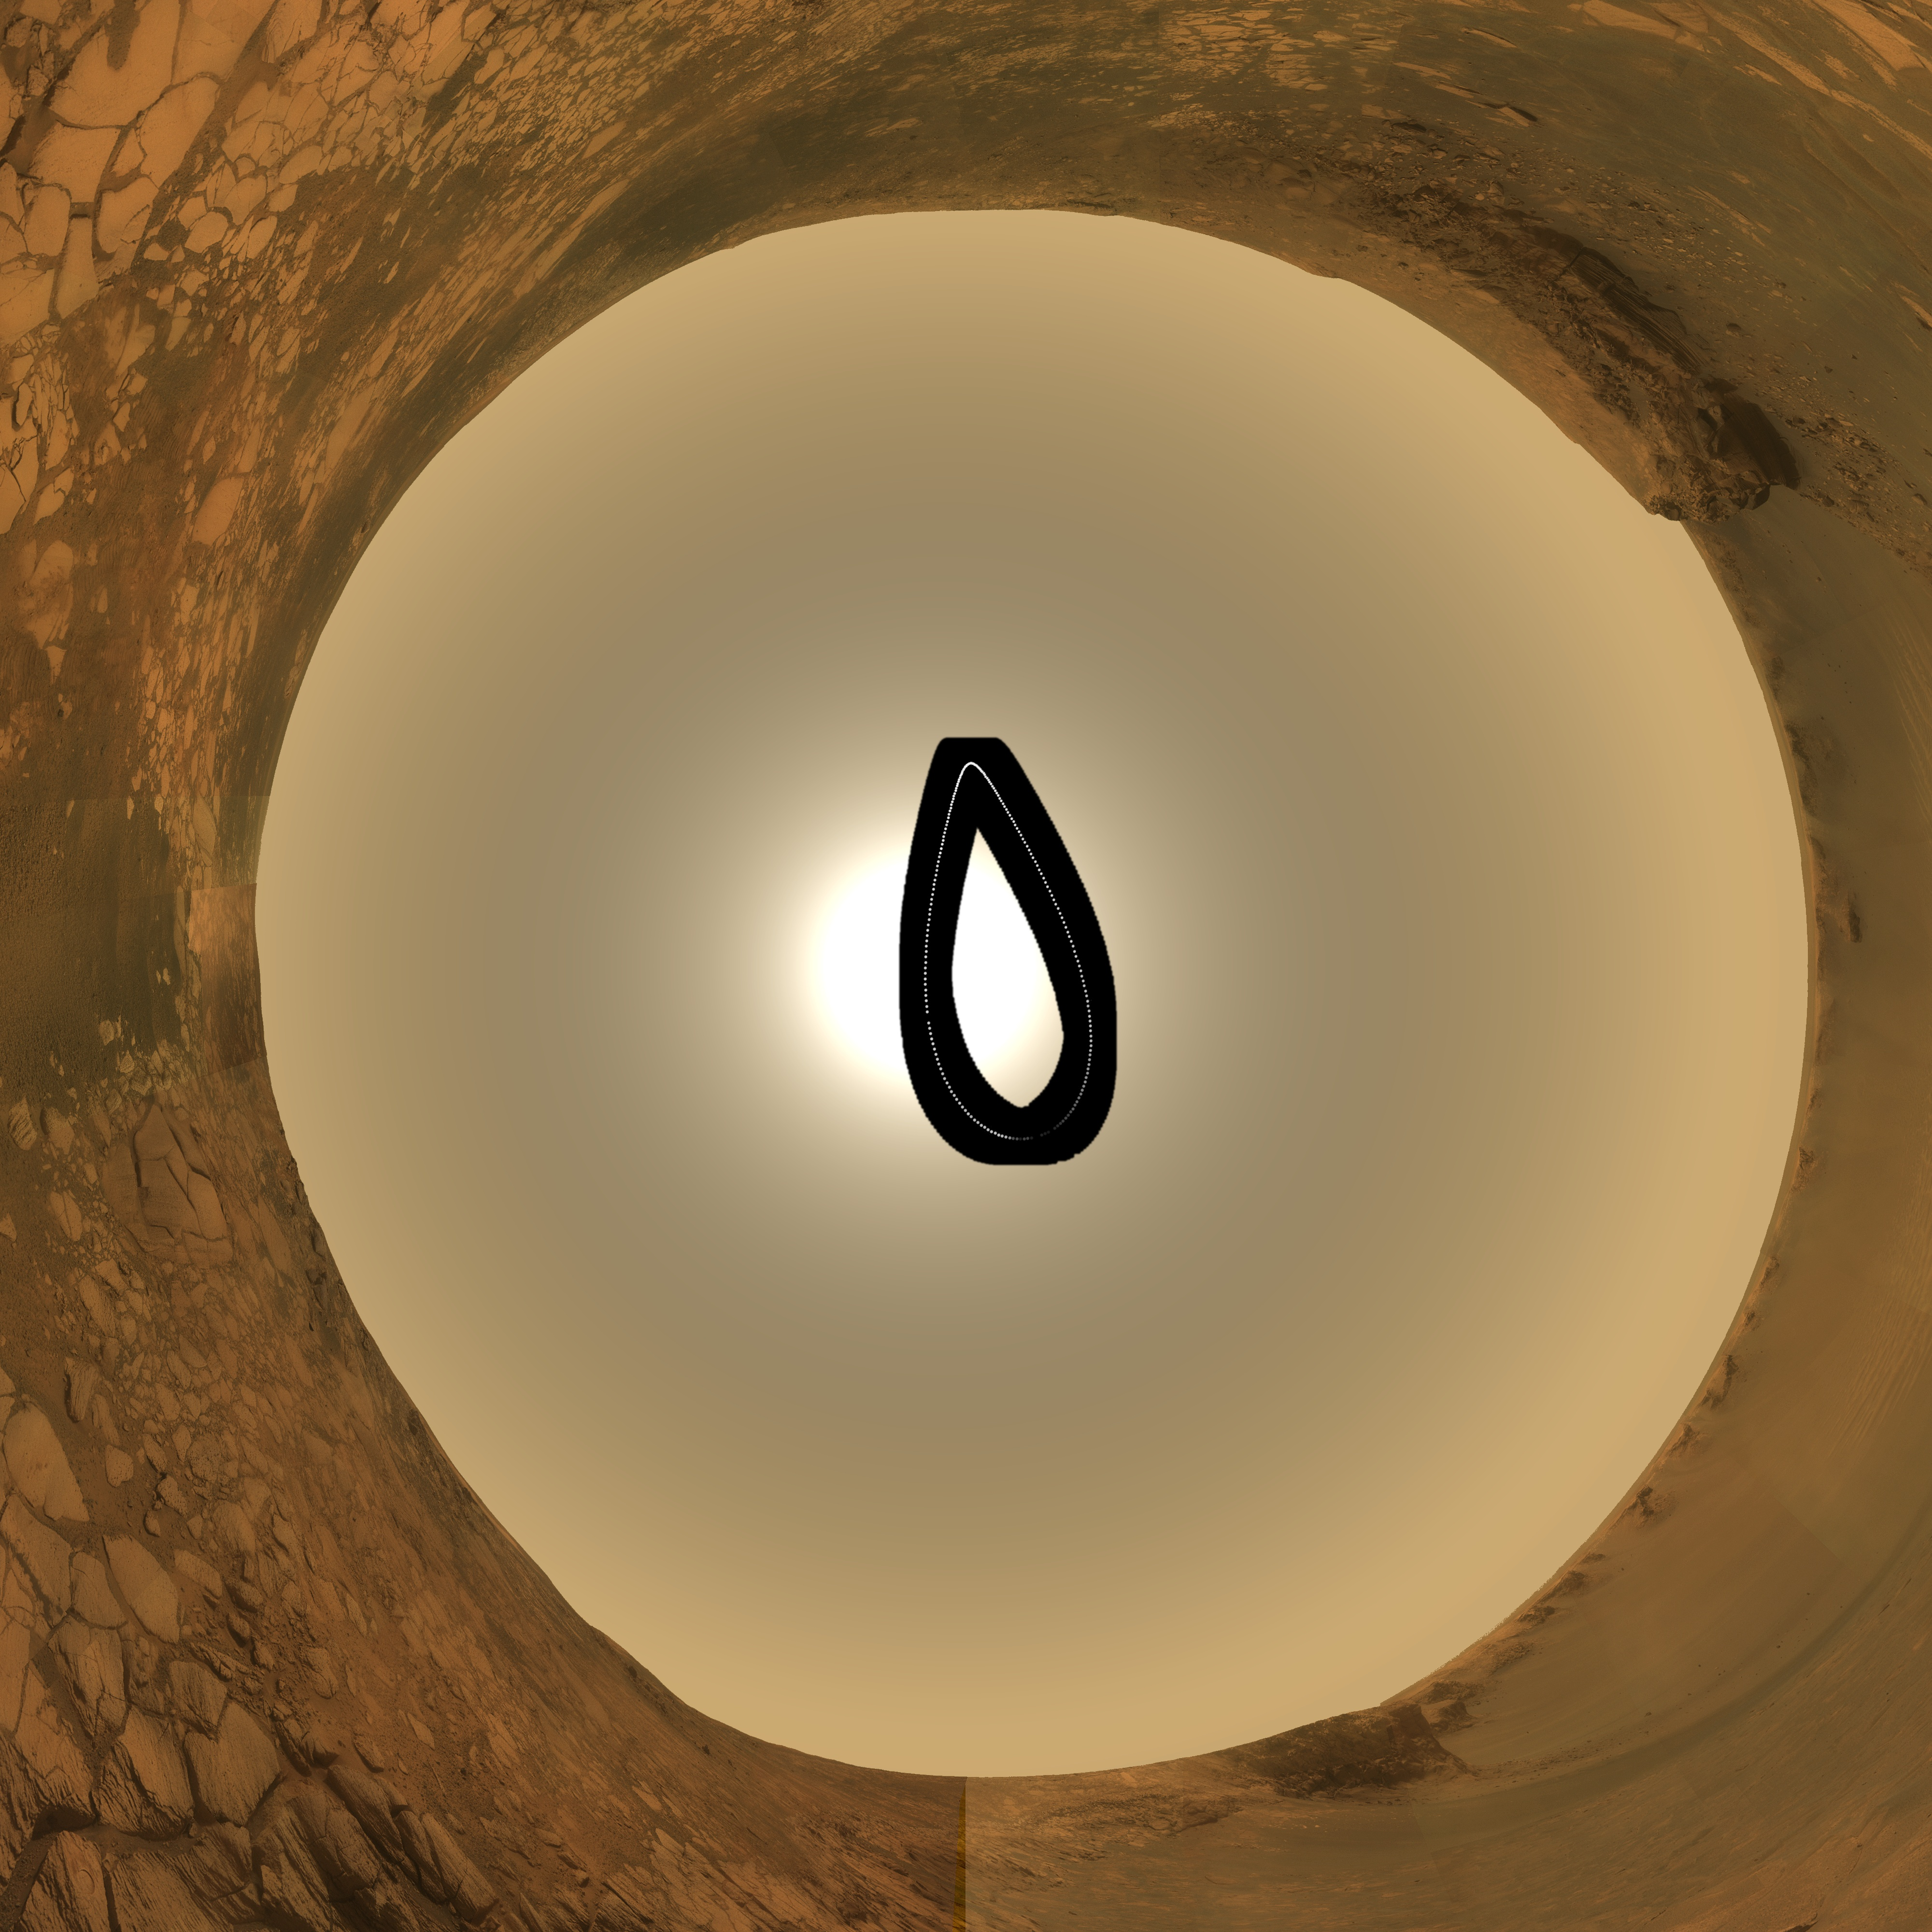
\includegraphics[width=0.6\textwidth]{Mars_Analemma.jpg}%
\caption[Rover Opportunitys Mars-Analemma.]{Rover Opportunitys Mars-Analemma aufgenommen zwischen 2006 und 2008 -- Bildcredit: NASA/JPL/Cornell/ASU/TAMU. }%
\label{abb:hm_Mars_Analemma}%
\end{figure}

Berechnen Sie f�r den Mars und die anderen Planeten die Zeitgleichungen und die Analemmas und versuchen Sie das aufgenommene Analemma zu reproduzieren.
Die Landekoordinaten k�nnen n�herungsweise mit $\varphi = -2.5\degree$ und $\lambda = 354.5\degree$ angenommen werden.\\
Die Werte f�r die Achsneigungen, Rotationsperioden und relativen Lagen der Rotationsachsen zur Ekliptik der einzelnen Planeten k�nnen Sie dem Internet bzw. \cite{JPL2020, Montenbruck1999} entnehmen.

\medskip 
%\hyperref[lsg:hm_Analemma_Mars]{\textcolor{blue} {$\rightarrow$ L�sungsvorschlag}}\\
\linklsg\\%\href{FingerUeb2_AB.pdf#lsg:hm_Analemma_Mars}{\textcolor{blue} {$\rightarrow$ L�sungsteil}}.\\
\noindent\rule[1ex]{\textwidth}{0.5pt}
\end{prob}

%-----------------------------------------------------------------------------------------------------------

\newpage
\begin{prob} %�bung23
\mittel{hm_sonnenaufgang_mars}{Sonnenaufgang Mars}
Zur Vorbereitung eines Marsfluges berechnen Sie mit Hilfe der einfachen Keplerl�sung die Sonnenaufg�nge f�r das Jahr 2030 auf dem Mars und zwar auf und am Fu�e des Olympus Mons (Koordinaten auf dem Mars:$18.65\degree$ N $, 133.8\degree W$).
Er hat eine Gipfelh�he von �ber $22\:\text{km}$ �ber dem mittleren Planetenniveau.
Der Mars rotiert in 24 Stunden und 37.4 Minuten um die eigene Achse (siderischer Tag).
In Bezug auf die Sonne ergibt sich daraus ein Marstag (auch Sol genannt) von 24 Stunden, 39 Minuten und 35 Sekunden.
Wie w�rde man einen Mars-Kalender in den Erdkalender umrechnen?
Benutzen Sie dazu die einfache Keplerl�sung f�r die Marsbahn.

\medskip 
%\hyperref[lsg:hm_sonnenaufgang_mars]{\textcolor{blue} {$\rightarrow$ L�sungsvorschlag}}\\
\linklsg\\%\href{FingerUeb2_AB.pdf#lsg:hm_sonnenaufgang_mars}{\textcolor{blue} {$\rightarrow$ L�sungsteil}}.\\
\noindent\rule[1ex]{\textwidth}{0.5pt}
\end{prob}


%-----------------------------------------------------------------------------------------------------------
\newpage
%%%-----------------------------------------------------------------------------------------------------------

\subsection{�bungen zu Monden, Kometen und Asteroiden}

\medskip

\begin{prob} %�bung24
\einfach{hm_MondbahnHelioz}{Heliozentrische Mondbahn}

Oft sieht man in popul�rwissenschaftlichen Darstellungen, dass die heliozentrische Mondbahn angeblich wegen der Erde eine Schleifenbewegung wie im rechten Teil der Abbildung \figref{hm_MondbahnHelioz} oder eine stark ausgepr�gte Wellenbahn wie im linken Bild ausf�hrt. Das ist aber keineswegs so, sondern es ergibt sich eine sehr schwach ausgepr�gte Wellenbahn, die nur wenig von der heliozentrischen Ellipsenbahn der Erde abweicht.\\
Begr�nden Sie das Ergebnis zun�chst anschaulich und rechnen Sie es numerisch nach. Unter welchen Bedingungen k�nnen Monde in unserem Sonnensystem eine Schleifenbahn wie in Abbildung \figref{hm_MondbahnHelioz} gezeigt ausf�hren?

\begin{figure}%

\includegraphics[width=\textwidth]{MondbahnHelioz.pdf}%
\caption[Formen von heliozentrischen Mondbahnen.]{Formen von heliozentrischen Mondbahnen. -- Bild nach \cite{Bastian2011}.}%
\label{abb:hm_MondbahnHelioz}%
\end{figure}

\medskip 
%\hyperref[lsg:hm_MondbahnHelioz]{\textcolor{blue} {$\rightarrow$ L�sungsvorschlag}}\\
\linklsg\\%\href{FingerUeb2_AB.pdf#lsg:hm_MondbahnHelioz}{\textcolor{blue} {$\rightarrow$ L�sungsteil}}.\\
\noindent\rule[1ex]{\textwidth}{0.5pt}
\end{prob}

%-----------------------------------------------------------------------------------------------------------

\begin{prob} %�bung25
\mittel{hm_kometen_asteroiden}{Kometen und Asteroiden}
W�hrend des Schreibens dieses Buches passierte der Komet Neowise den Bereich zwischen Erdbahn und Sonne. Das gab Anlass f�r diese Aufgabe.
\begin{enumerate}
	\item Komet Neowise: Berechnen Sie die Bahn des Kometen Neowise und stellen Sie diese in zwei Projektionen f�r die Gesamtbahn und den Zeitabschnitt um den Periheldurchgang bzw. die Erdbahnkreuzung dar.
          Geben Sie die geozentrisch-�quatorialen Koordinaten und die topozentrisch-horizontalen Koordinaten f�r den 12.07.2020 21:00 UTC an.
          Der Beobachtungsort lag bei: $48.867164\degree$N, $10.223733\degree$O.
          In welchem Sternbild war Neowise zu sehen?
        \item Komet Halley: Berechnen Sie die Beobachtungsdaten f�r den Kometen Halley f�r 1758 und 1986 jeweils in der N�he des Perihels und der Erdn�he und vergleichen Sie diese (Tabelle \ref{tab:hm_parameter_halley_alt-neu}, \mscr{} \mlhmref{KometenHalley.m}).
	\item Der gro�e Komet von 1680 \cite{Stoyan2013,Krause2013}: Anfang Dezember 1680 n�herte sich der gro�e Komet immer mehr der Sonne und am 18. Dezember ging er durch seinen sonnenn�chsten Punkt (Perihel).
          Er entwickelte eine solche Helligkeit, dass er am Taghimmel neben der Sonne zu sehen war.
          Die Sch�nheit des Kometen wurde durch einen imposanten Schweif verst�rkt.
          John Flamsteed\indexp{Flamsteed, John}\footnote{John Flamsteed (1646--1719) war ein englischer Astronom und seit 1675 der erste \emph{Astronomer Royal} des englischen K�nigshauses (vor Halley). Er schrieb \ua eine wichtige Abhandlung �ber die Bestimmung der Zeitgleichung, sammelte die Daten von rund 2800 sichtbaren Sternen und lag eher unverschuldet mit Newton in einem Urheberrechtsstreit.} berichtete, dass dieser sich am 21.~Dezember mit der Breite des Vollmonds senkrecht vom Horizont bis fast zum Zenit erstreckte.
          Der Kopf des Kometen war so hell wie ein Stern erster Gr��e.
        Am 28.~Dezember erreichte der Schweif nach Robert Hooke\indexp{Hooke, Robert}\footnote{Robert Hooke (1635--1703) war ein englischer Naturforscher, der haupts�chlich durch das nach ihm benannte Elastizit�tsgesetz bekannt ist. 
	Mit Newton verband Hooke eine tiefe Abneigung.
        Newton\indexp{Newton, Sir Isaac} lehnte jegliche Anerkennung f�r Hookes Beitr�ge ab, die Newton zu seiner mathematische Formulierung der Bewegungs- und Gravitationsgesetze benutzte.}
        in England eine L�nge von $90$\textdegree\ und reichte damit �ber das halbe Firmament.
        Man kann sich vorstellen, welche ungeheure Wirkung der Komet im Jahre 1680 auf die Menschen hatte.
        Der Komet wurde zuletzt am 19.03.1681 beobachtet.
        Die Bahnparameter konnte man ableiten und diese finden sich in Tabelle \ref{tab:hm_parameter_kometen} im Tabellenanhang.
        Berechnen Sie die Beobachtungsdaten f�r Greenwich und erkl�ren Sie, warum der Komet so beeindruckend war.
	\item Asteroiden: Berechnen Sie die Bahn f�r die in Tabelle \ref{tab:hm_parameter_asteroide} angegebenen Asteroiden und stellen Sie diese f�r die Jahre 2021 und 2022 mit den Bahnen der inneren Planeten dar.
          Wann befinden sie sich in Opposition zur Erde, wann gibt es eine optimale Beobachtungschance?
          Was sind dann die geozentrisch-�quatorialen Koordinaten?
          Wie gro� ist die Gefahr einer Kollision mit dem Asteroiden 231937?
\end{enumerate}
Stellen Sie die Bahnen f�r die Teilaufgaben 1. bis 4. jeweils heliozentrisch und in Perihel- und Erdn�he in einem $\alpha,\delta$-Diagramm dar.

\medskip 
%\hyperref[lsg:hm_kometen_asteroiden]{\textcolor{blue} {$\rightarrow$ L�sungsvorschlag}}\\
\linklsg\\%\href{FingerUeb2_AB.pdf#lsg:hm_kometen_asteroiden}{\textcolor{blue} {$\rightarrow$ L�sungsteil}}.\\
\noindent\rule[1ex]{\textwidth}{0.5pt}
\end{prob}

%-----------------------------------------------------------------------------------------------------------

\begin{prob} %�bung26
\schwierig{hm_verweildauer_komet_erdbahn}{Kometen und Meteoriten\index{Meteorit}}
Dies ist eine Aufgabe mit Bezug zur Region, in der einer der Autoren lebt. (nach \cite{Quetz2017})
\begin{enumerate}
	\item K�nnen Sie eine Erkl�rung geben, warum die meisten Kometen nur ca. 1--2 Monate zu sehen sind?
          Berechnen Sie dazu zun�chst analytisch die Zeit f�r einen Kometen mit Perihel $0.1\!<\!q\!<\!0.8\:$AE und einer \gls{inklination} von $\approx\!0$.
          Verk�rzt oder verl�ngert sich die Beobachtungszeit beim �bergang zu starken Bahnneigungen (z.B. Donati 1856, Gro�er Komet 1689)?
          �berpr�fen Sie Ihre Absch�tzungen mit \mscr{} \mlhmref{KometenBahnen.m} \bzw \mlhmref{KometenZeity.m}.
	\item Berechnen Sie die Aufschlaggeschwindigkeit eines Kometen/Meteoriten auf der Erde unter Annahme der Kenntnis seiner Bahnelemente $a_\text{K}, e_\text{K}, i_\text{K}$.
	\item K�nnen Sie aus den Durchmessern des N�rdlinger Ries (24 km) und des Steinheimer Beckens (3.8 km)\footnote{Beide Einschlagkrater entstanden vor ca.\ 14--15 Millionen Jahren durch Meteore, wobei Oberkochen (gelber Stern auf der Karte) gl�cklicherweise nicht getroffen wurde.} auf Basis der sogenannten Shoemaker Formel \cite{Shoemaker1979} eine Absch�tzung f�r die kinetische Energie des Meteoriten beim Aufschlag machen?
	\begin{figure}%
\includegraphics[width=\textwidth]{NoerdlingenSteinheim.pdf}%
\caption[Satellitenkarte mit zwei Einschlagkratern.]{Satellitenkarte mit den beiden Einschlagkratern des N�rdlinger Ries und Stein\-heimer Beckens.}%
\label{abb:hm_NoerdlingenSteinheim}%
\end{figure}
	Die Shoemaker\footnote{Eugene Merle Shoemaker (1928--1997) war ein US-amerikanischer Geologe, Impaktforscher und Astronom. Bekannt wurde er als Mitentdecker und Namensgeber des Kometen Shoemaker-Levy 9 (mit seiner Frau Carolyn Shoemaker und David H. Levy). Er konnte in seinen geologischen Forschungen nachweisen, dass der Barringer-Meteorkrater in den USA und tats�chlich auch das N�rdlinger Ries durch einen Meteoriteneinschlag entstanden sind. Er war 1969 auch Chefwissenschaftler der Apollo-11-Mission.}\indexp{Shoemaker, Eugene Merle} Formel stellt einen Zusammenhang zwischen Kraterdurchmesser $D$ und kinetischer Aufprallenergie $E_\text{kin}$ her, wobei $E_\text{kin}$ in kt TNT-�quivalent ausgegeben wird und $D$ in km:
	\begin{equation}
	D=0.074 \:\kappa\: E_\text{kin}^{1/3.4}  \;. \label{eq:hm_Shoemaker1979}
	\end{equation}
Dabei ist der Parameter $\kappa\!=\!1.3$ f�r Durchmesser $D\!\geq\! 3\:\text{km}$.
Geben Sie unter Benutzung der minimalen und maximalen Aufschlaggeschwindigkeit aus Aufgabenteil 2 den m�glichen Bereich f�r die Durchmesser der Meteoriten an.
Die mittlere Dichte ist $\rho\!=\!2.8 \:\text{g}/\text{cm}^3$ (\figref{hm_NoerdlingenSteinheim}).\\
K�nnen Sie eine plausible Herleitung/Absch�tzung f�r die Shoemaker  Formel geben? (�bung nach \cite{Quetz2017})
\item K�nnen Sie die Vermutung best�tigen, dass es sich bei den beiden nahe beieinander liegenden Einschlagkratern um das Ergebnis des Einschlags eines Doppel-Planetoiden\index{Planetoiden} (bzw. eines Planetoiden mit seinem Mond) handelt?
  Benutzen Sie f�r Ihre Argumentation das Ergebnis von Aufgabenteil 3.
\end{enumerate}
\medskip 
%\hyperref[lsg:hm_verweildauer_komet_erdbahn]{\textcolor{blue} {$\rightarrow$ L�sungsvorschlag}}\\
\linklsg\\%\href{FingerUeb2_AB.pdf#lsg:hm_verweildauer_komet_erdbahn}{\textcolor{blue} {$\rightarrow$ L�sungsteil}}.\\
\noindent\rule[1ex]{\textwidth}{0.5pt}
\end{prob}

%-----------------------------------------------------------------------------------------------------------

\begin{prob} %�bung27
\einfach{hm_Doppelstern}{Doppelstern-System - Vergleich numerische und analytische L�sung}
Vergleichen Sie die numerische Rechnung f�r ein Doppelsternsystem mit der analytischen Rechnung. Variieren Sie die Genauigkeiten im Solver f�r die Differentialgleichungen. Stellen Sie die Energie, die Bewegung des Schwerpunktes und den Drehimpuls �ber die Zeit dar. Welche Aussagen k�nnen Sie machen?

\medskip 
%\hyperref[lsg:hm_Doppelstern]{\textcolor{blue} {$\rightarrow$ L�sungsvorschlag}}\\
\linklsg\\%\href{FingerUeb2_AB.pdf#lsg:hm_Doppelstern}{\textcolor{blue} {$\rightarrow$ L�sungsteil}}.\\
\noindent\rule[1ex]{\textwidth}{0.5pt}
\end{prob}

%-----------------------------------------------------------------------------------------------------------

\begin{prob} %�bung28
\mittel{hm_Sonnensystem}{Sonnensystem - Numerische, Kepler- und JPL-Berechnung}
Erstellen Sie ein \matlab-Programm, welches die Bewegung des gesamten Sonnensystems auf Basis der Newtonschen Bewegungsgleichungen im Schwerpunktsystem berechnet und vergleichen Sie die so berechneten Koordinaten mit der ZKP-Kepler-L�sung (\vgl \mscr{}~ \mlhmref{InnerePlaneten.m}) und mit den Berechnungen des JPL \cite{JPL2020}. Die Anfangswerte k�nnen Sie sich vom JPL beschaffen.\\
Betrachten Sie dabei das Sonnensystem in einem Inertialsystem. Typischerweise nimmt man das \textit{International Celestial Reference Frame} (ICRF) \cite{Park2021,JPL2020}. Dieses \KOS wird durch die Positionen von Quasaren und anderen extragalaktischen Objekten mit starker Radiostrahlung definiert. Gewonnen werden diese Positionen durch die sogenannte VLBI\footnote{\textit{Very Long Baseline Interferometry (VLBI)} ist eine Methode der Radioastronomie f�r Messungen mit h�chster r�umlicher Aufl�sung und Positionsgenauigkeit.}. Der Koordinatenursprung des ICRF ist der Schwerpunkt (das Baryzentrum) des Sonnensystems (\textit{Solar System Barycenter SSBC}).

\medskip 
%\hyperref[lsg:hm_Sonnensystem]{\textcolor{blue} {$\rightarrow$ L�sungsvorschlag}}\\
\linklsg\\%\href{FingerUeb2_AB.pdf#lsg:hm_Sonnensystem}{\textcolor{blue} {$\rightarrow$ L�sungsteil}}.\\
\noindent\rule[1ex]{\textwidth}{0.5pt}
\end{prob}


%-----------------------------------------------------------------------------------------------------------

\begin{prob} %�bung29
\mittel{hm_Dreifachstern}{Dreik�rper-System - L�sung f�r 3 identische Massen}
Es ist immer wieder erstaunlich, wie neue interessante Effekte aus den Bewegungsgleichungen unter dem Einfluss der Gravitation gefunden werden k�nnen. Erst im Jahr 1993 \bzw 2000 gelang es Wissenschaftlern nachzuweisen, dass drei identische Massen, die sich allein unter dem gegenseitigen Einfluss der Gravitation befinden auf einer achtf�rmigen Kurve bewegen \cite{Moore1993, Chenciner2000}.\\
\begin{enumerate}
\item Zeigen Sie numerisch durch L�sung der Bewegungsgleichungen, dass bei geeignet gew�hlten Anfangsbedingungen diese Bahnform tats�chlich erhalten werden kann und auch stabil ist. W�hlen Sie den koplanaren Fall aus, in welchem die Massen sich anf�nglich bei $[-x_0, 0],\, [0, 0],\ [+x_0, 0]$ befinden und gehen Sie von einem Anfangs-Gesamtimpuls von 0 aus, in dem Sie die beiden �u�eren Massen in entgegengesetzte Richtung der mittleren Masse jeweils mit $v_0/2$ starten lassen. Variieren Sie den Winkel von $\vec{v}_0$ zur $x$-Achse\footnote{Eine allgemeinere Betrachtung zum Auffinden von geeigneten Anfangsbedingungen findet sich in \cite{Suvakov2014}}.
\item Schon l�nger bekannt ist die L�sung f�r das Dreik�rperproblem, bei dem sich die drei identischen Massen an den Eckpunkten eines gleichseitigen Dreiecks befinden. Hier kann man die Bewegungsgleichungen sogar analytisch l�sen. Erstellen Sie auch ein \matlab-Programm f�r die numerische L�sung. Wenn Sie dieses f�r l�ngere Zeiten ausf�hren, werden Sie sehen, dass die L�sung instabil und sogar chaotisch wird (\vgl Band I). Kleinste St�rungen (in unserem Fall numerische Rundungen) f�hren zur Instabilit�t. K�nnen Sie das auch analytisch begr�nden? Sehen Sie dazu auch die Rechnungen im \kap{Stabile_Bahnen} an.
\end{enumerate}
\medskip 
%\hyperref[lsg:hm_Dreifachstern]{\textcolor{blue} {$\rightarrow$ L�sungsvorschlag}}\\
\linklsg\\%\href{FingerUeb2_AB.pdf#lsg:hm_Dreifachstern}{\textcolor{blue} {$\rightarrow$ L�sungsteil}}.\\
\noindent\rule[1ex]{\textwidth}{0.5pt}
\end{prob}

%-----------------------------------------------------------------------------------------------------------

\begin{prob} %�bung30
\schwierig{hm_Tempel1_SwiftTuttle}{Kometen im Sonnensystem -- Kollision mit der Erde?}
Wir haben im \kap{kometen} gezeigt, wie man �ber die L�sung der Kepler-Gleichung bei (n�herungsweise) bekannten Bahnparametern die Bahnen der Kometen bestimmen kann.
Jedoch unterliegen die Bahnen der Kometen im von der Sonne weiter entfernten Bereich den Gravitationskr�ften der �u�eren Planeten und werden dadurch gest�rt.
\begin{enumerate}
\item Es gibt Vermutungen, dass der Komet Swift-Tuttle, der am 12. Dezember 1992 um 21:23 UT sein Perihel hatte, m�glicherweise bei seiner Wiederkehr im Jahre 2126 die Erde treffen k�nnte. Die Bahnparameter des Kometen konnten wie folgt bestimmt werden (\cite{JPL2020}):\\
\begin{align*}
a      &=  26.09206949782666 \:\text{AE} \\
e      &=   0.9632257550460384 \\
i      &= 113.4538169971712\degree\\
\omega &= 152.9821676305871\degree \\
\Omega &= 139.3811920815948\degree \\
T_\text{Per}  &= 1992-\text{Dec}-11.9997845562 \\
q      &= 0.9595161550688684\:\text{AE} ~~ \text{(Perihelabstand)}\\
M      &= 7.631696167124793 \degree ~~ \text{am} ~~2450000.5 ~~\text{(1995-Oct-10.0000000)}\\
n      &= 0.007395053\,\mathrm{a}^{-1}~~ \text{(mittlere Bewegung)}             
\end{align*}  

M�ssen wir uns wegen einer m�glichen Kollision Sorgen machen? 
Vergleichen Sie Ihr Ergebnis unter Benutzung des \matlab-Programms aus \probref{hm_Sonnensystem} wiederum mit den Berechnungen des JPL \cite{JPL2020} und den L�sungen aus der Kepler-Gleichung, wie \zb in \probref{hm_kometen_asteroiden}. Was k�nnen Sie daraus �ber die Bahn des Kometen sagen? 

\item Berechnen Sie unter Benutzung des \matlab-Programms aus \probref{hm_Sonnensystem} und den L�sungen aus der Kepler-Gleichung, wie \zb in \probref{hm_kometen_asteroiden} die Bahn des Kometen 9P/Tempel 1 f�r die Jahre 2016 und 2022 und vergleichen Sie diese. 
Die Bahnparameter des Kometen konnten wie folgt bestimmt werden (\cite{JPL2020}):\\
\begin{align*}
a      &=  3.146289866273702 \:\text{AE} \\
e      &=   0.509730344014817\\
i      &= 10.47332142324269\degree\\
\omega &= 179.1945054082475\degree \\
\Omega &= 68.75570898836558\degree \\
T_\text{Per} &= 2016-\text{Aug}-02.5673848162 \\
q      &= 1.542530450367674\:\text{AE} ~~ \text{(Perihelabstand)}\\
M      &= 333.055652021317 \degree ~~ \text{am} ~~2457450.5 ~~\text{(2016-Mar-03.0000000)}\\
n      &= 0.176606212 \,\mathrm{a}^{-1}~~ \text{(mittlere Bewegung)}               
\end{align*}  
\end{enumerate}

\medskip 
%\hyperref[lsg:hm_Tempel1_SwiftTuttle]{\textcolor{blue} {$\rightarrow$ L�sungsvorschlag}}\\
\linklsg\\%\href{FingerUeb2_AB.pdf#lsg:hm_Tempel1_SwiftTuttle}{\textcolor{blue} {$\rightarrow$ L�sungsteil}}.\\
\noindent\rule[1ex]{\textwidth}{0.5pt}
\end{prob}

%-----------------------------------------------------------------------------------------------------------

\begin{prob} %�bung31
\einfach{hm_lichtlaufzeit}{Lichtlaufzeit, Unterschied zwischen ET und UT}
Leiten Sie Gleichung \eqref{eq:hm_scheinbare_koord_B} ab und sch�tzen Sie die Effekte der Lichtlaufzeit auf die Beobachtungskoordinaten f�r die Kometen Halley und Neowise in Periheln�he ab.
Nutzen Sie dabei f�r die Berechnung der Geschwindigkeiten die vis-viva-Gleichung.
In welcher Zeit $\Delta t$ verliert man bei Einstellung auf die berechneten Koordinaten den Kometen aus dem Bildfeld der Vollformat-CCD Kamera?
Diese befinde sich im Zwischenfokus des �quatorial-montierten und mitgef�hrten Teleskops mit einer Brennweite von $f\!=\!2500\:$mm.
Berechnen Sie auch welchen Fehler man begeht, wenn man bei der Berechnung der Position nach der Kepler-Gleichung anstelle der ET die Weltzeit UT benutzt.
Befindet sich das Objekt dann noch im eingestellten Sichtfeld des Teleskops?

\medskip 
%\hyperref[lsg:hm_lichtlaufzeit]{\textcolor{blue} {$\rightarrow$ L�sungsvorschlag}}\\
\linklsg\\%\href{FingerUeb2_AB.pdf#lsg:hm_lichtlaufzeit}{\textcolor{blue} {$\rightarrow$ L�sungsteil}}.\\
\noindent\rule[1ex]{\textwidth}{0.5pt}
\end{prob}

%-----------------------------------------------------------------------------------------------------------
\newpage
%%%-----------------------------------------------------------------------------------------------------------
\subsection{�bungen zu Gezeiten}

\medskip

%-----------------------------------------------------------------------------------------------------------

\begin{prob} %�bung32
\mittel{hm_rochelimit}{Zur Herleitung des Roche-Limits}\index{Roche-Limit}
Berechnen Sie unter der Annahme, dass ein Asteroid/Komet eine Dichte von ca. $\SI{500}{\kg\per\cubic\metre}$ hat, ab welcher Entfernung er beim Passieren der Jupiterbahn von dem Planeten zerrissen wird. \\
Vergleichen Sie Ihr Ergebnis mit den Messungen zum Kometen Shoemaker-Levy (\vgl \kap{hm_numerische_proced}) und auch mit der Hill-Sph�re $r_\text{H}$ (\vgl \probref{hm_hill_sphere}) des Jupiters. \\
Berechnen Sie die Roche-Grenzen f�r die Planeten unseres Sonnensystems und diskutieren Sie diese im Vergleich zu den Hill-Sph�ren.

\medskip 
%\hyperref[lsg:hm_rochelimit]{\textcolor{blue} {$\rightarrow$ L�sungsvorschlag}}\\
\linklsg\\%\href{FingerUeb2_AB.pdf#lsg:hm_rochelimit}{\textcolor{blue} {$\rightarrow$ L�sungsteil}}.\\
\noindent\rule[1ex]{\textwidth}{0.5pt}
\end{prob}


%-----------------------------------------------------------------------------------------------------------

\begin{prob} %�bung33
\einfach{hm_gezeiten01}{Tidenhub in einem Wasserglas}
\begin{enumerate}
	\item Wie gro� ist der Tidenhub $\Delta h$ in einem Wasserglas (Durchmesser $\SI{10}{\cm}$) und in einem gro�en See (\zb Bodensee) (Durchmesser $\SI{50}{\km}$)? 
	\item Gibt es eine Abh�ngigkeit von der geographischen Breite?
\end{enumerate}

\medskip 
%\hyperref[lsg:hm_gezeiten01]{\textcolor{blue} {$\rightarrow$ L�sungsvorschlag}}\\
\linklsg\\%\href{FingerUeb2_AB.pdf#lsg:hm_gezeiten01}{\textcolor{blue} {$\rightarrow$ L�sungsteil}}.\\
\noindent\rule[1ex]{\textwidth}{0.5pt}
\end{prob}

%-----------------------------------------------------------------------------------------------------------

\begin{prob} %�bung34
\einfach{hm_gezeiten02}{Bewegung der Erde im Erde-Mond-System}
Zeigen Sie mit einer \matlab-Computersimulation, dass jeder Punkt der Erde innerhalb eines synodischen Monats eine Kreisbewegung um sein eigenes Umlaufzentrum ausf�hrt. \\

\medskip 
%\hyperref[lsg:hm_gezeiten02]{\textcolor{blue} {$\rightarrow$ L�sungsvorschlag}}\\
\linklsg\\%\href{FingerUeb2_AB.pdf#lsg:hm_gezeiten02}{\textcolor{blue} {$\rightarrow$ L�sungsteil}}.\\
\noindent\rule[1ex]{\textwidth}{0.5pt}
\end{prob}

%-----------------------------------------------------------------------------------------------------------
\newpage
\begin{prob} %�bung35
\einfach{hm_gezeiten03}{Newtonsche Gleichgewichtstheorie}
Abstand zwischen zwei Hochwassern und Tidenhub bei verschiedenen Deklinationen:
\begin{enumerate}
	\item Berechnen Sie den mittleren zeitlichen Abstand zwischen zwei Hochwassern im Gezeitensystem Erde-Mond.
	\item Berechnen Sie den Tidenhub f�r zwei aufeinanderfolgende Mondtiden f�r eine geographische Breite $\varphi$ und bei der minimalen und maximalen Monddeklination $\delta_\text{M}$.
	\item Berechnen Sie den Tidenhub am �quator f�r zwei aufeinanderfolgende Tiden bei Vollmond f�r verschiedene Deklinationen des Mondes zur Wintersonnenwende. Vergleichen Sie das Ergebnis mit den Beobachtungen von Dezember 2022 im Indischen Ozean (\figref{hm_DiegoGarciaTideTable}).
	\item Erkl�ren Sie das Auftreten von drei Amphidromiepunkten in der Nordsee.
\end{enumerate}
\begin{figure}%
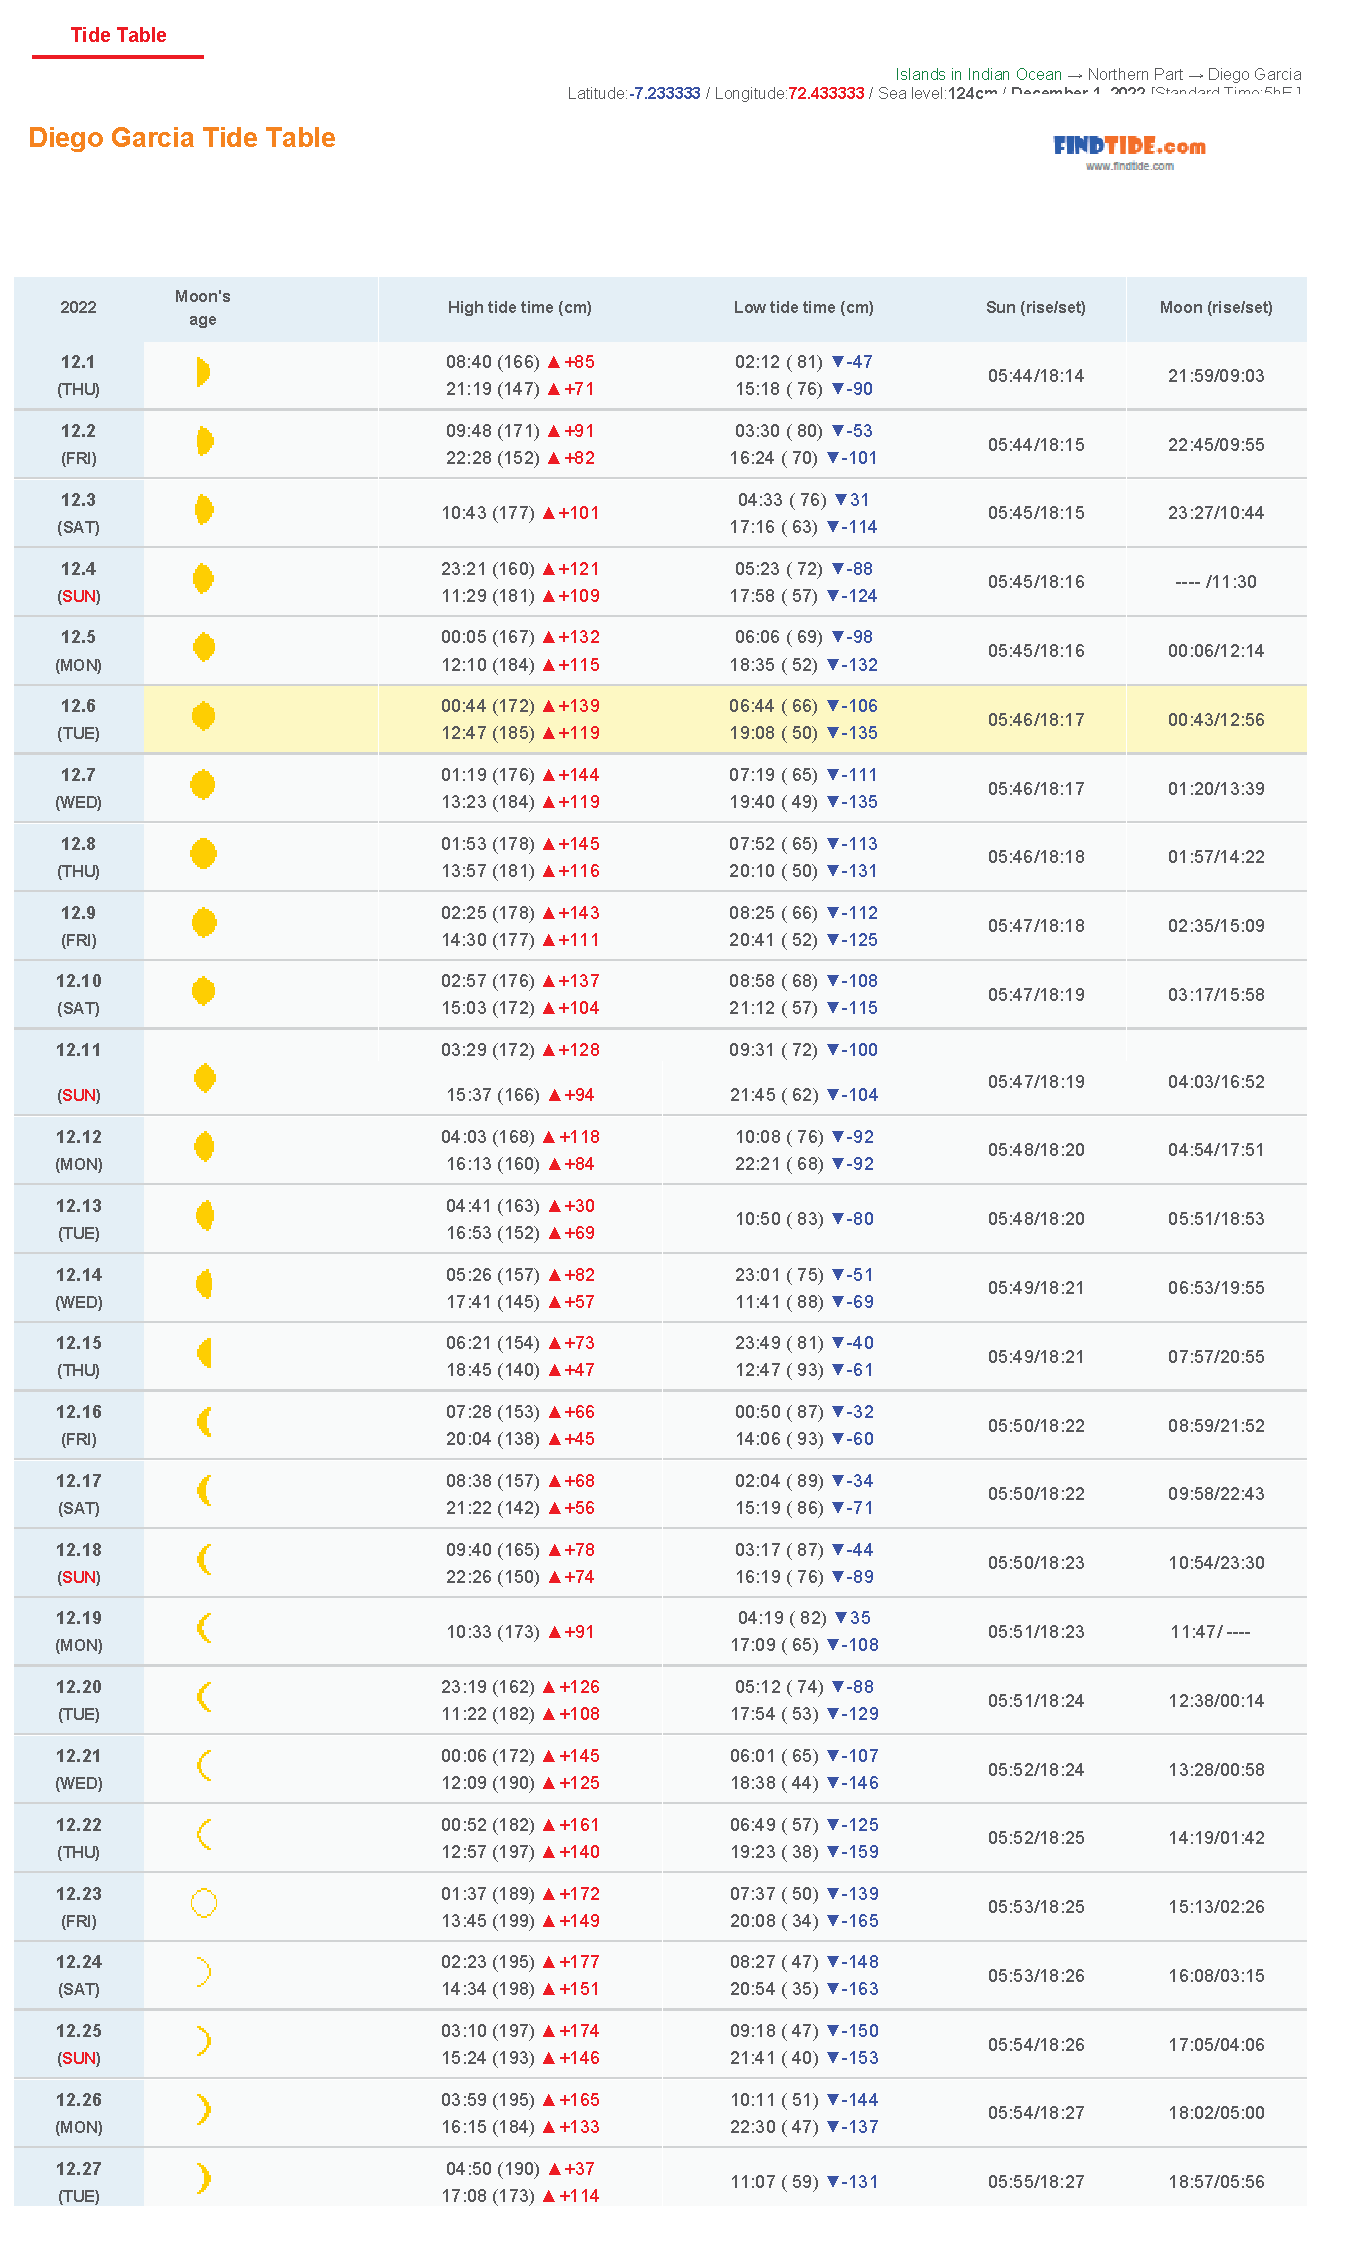
\includegraphics[width=\textwidth]{DiegoGarciaTideTable.pdf}%
\caption{Tiden-Tabelle von Diego Garcia im Indischen Ozean.}
	\label{abb:hm_DiegoGarciaTideTable}
\end{figure}
%\hyperref[lsg:hm_gezeiten03]{\textcolor{blue} {$\rightarrow$ L�sungsvorschlag}}\\
\linklsg\\%\href{FingerUeb2_AB.pdf#lsg:hm_gezeiten02}{\textcolor{blue} {$\rightarrow$ L�sungsteil}}.\\
\noindent\rule[1ex]{\textwidth}{0.5pt}
\end{prob}

%-----------------------------------------------------------------------------------------------------------
\newpage
\begin{prob} %�bung36
\einfach{hm_gezeiten04}{Gezeitenellipsoid}
\begin{enumerate}
	\item Berechnen Sie Form des Gezeitenellipsoids und die relativen H�hen nach der Newtonschen Gleichgewichtstheorie. \\
	\item Berechnen Sie Form des Gezeitenellipsoids nach der Potentialtheorie entsprechend \kap{hm_potentialtheorie}. \\

\end{enumerate}
\medskip 
%\hyperref[lsg:hm_gezeiten04]{\textcolor{blue} {$\rightarrow$ L�sungsvorschlag}}\\
\linklsg\\%\href{FingerUeb2_AB.pdf#lsg:hm_gezeiten04}{\textcolor{blue} {$\rightarrow$ L�sungsteil}}.\\
\noindent\rule[1ex]{\textwidth}{0.5pt}
\end{prob}

%-----------------------------------------------------------------------------------------------------------
%\newpage
\begin{prob} %�bung37
\mittel{hm_gezeiten05}{Wasserkanal nach Airy}
Einfaches Modell zur Dynamischen Theorie: 
Zeigen Sie, dass die �berlagerung der beiden Einzelschwingungen $q_1\lk t\rk$ und $q_2\lk t\rk$ in dem Wasserkanal nach Airy f�r die Summe der erzeugten St�rungen (H�hen�nderungen im Kanal)
	\[   \Delta h = q_1\lk t\rk \cos 2\theta + q_2\lk t\rk \sin 2\theta  = \hat{q}\,\cos\lek 2\,\lk \omega_\text{E}t-\delta/2-\theta\rk\rek \,. 
	\]
eine gute N�herung f�r die am �quator an einem Ort $R_\text{E},\, \theta$ beobachteten Gezeiten darstellt. Hierin ist $\theta$ ein beliebiger L�ngengrad und $\delta$ eine zu berechnende Phasenverschiebung zwischen der direkten Linie Erdmittelpunkt-Mond und dem sich ausbildenden und zu berechnenden Maximum der Gezeitenwelle, $\omega_\text{E}$ die Kreisfrequenz der Erdrotation. Nehmen Sie f�r die Gezeitenwelle im Kanal eine Umlauffrequenz $\omega_0$ und eine D�mpfung $\gamma$ an.

\medskip 
%\hyperref[lsg:hm_gezeiten05]{\textcolor{blue} {$\rightarrow$ L�sungsvorschlag}}\\
\linklsg\\%\href{FingerUeb2_AB.pdf#lsg:hm_gezeiten05}{\textcolor{blue} {$\rightarrow$ L�sungsteil}}.\\
\noindent\rule[1ex]{\textwidth}{0.5pt}
\end{prob}


%-----------------------------------------------------------------------------------------------------------

\begin{prob} %�bung38
\mittel{hm_gezeiten06}{Gezeitenreibung - Hantelmodell}
Berechnen Sie die Gezeitenreibung und damit die zeitliche Entwicklung im Erde-Mond-System. Nehmen Sie f�r das Gezeitenellipsoid in \figref{hm_gezeiten08} eine Hantel als einfaches Modell 
der Masseverteilung an.

\medskip 
%\hyperref[lsg:hm_gezeiten06]{\textcolor{blue} {$\rightarrow$ L�sungsvorschlag}}\\
\linklsg\\%\href{FingerUeb2_AB.pdf#lsg:hm_gezeiten06}{\textcolor{blue} {$\rightarrow$ L�sungsteil}}.\\
\noindent\rule[1ex]{\textwidth}{0.5pt}
\end{prob}


%-----------------------------------------------------------------------------------------------------------

\begin{prob} %�bung39
\mittel{hm_gezeiten06a}{Gezeitenreibung - Auswirkung Mond}
Nat�rlich erzeugt auch das Gravitationsfeld der Erde auf dem Mond Gezeitenberge und ebenso eine Gezeitenreibung, falls es  eine Zeitverschiebung zwischen dem Gezeitenberg auf dem Mond und der Erde-Mond-Linie gibt. Dies w�rde v�llig analog wie bei der Erde zu einer Verlangsamung der Mondeigenrotation $\Omega_\text{M}$ f�hren, solange bis diese mit der Umlaufwinkelgeschwindigkeit um die Erde �bereinstimmt. Berechnen Sie die Verlangsamungsrate der Mondeigenrotation unter folgenden Annahmen:
\begin{align*}
    \Omega_\text{M}\lk 0\rk &= 4\omega_\text{M} &&\text{(initiale Eigenrotation 4x der heutigen Umlauffrequenz)}\\
    \mu_\text{M} &\approx 50 && \text{(effektive Festigkeit)}\\
    \delta &= 0.01\,\text{rad}
\end{align*}
Hinweis: Das sind nat�rlich nur sehr grobe Annahmen, der Leser m�ge das Ergebnis �ber eine gr��ere Bandbreite von Parametern darstellen. \\

\medskip 
%\hyperref[lsg:hm_gezeiten06a]{\textcolor{blue} {$\rightarrow$ L�sungsvorschlag}}\\
\linklsg\\%\href{FingerUeb2_AB.pdf#lsg:hm_gezeiten06a}{\textcolor{blue} {$\rightarrow$ L�sungsteil}}.\\
\noindent\rule[1ex]{\textwidth}{0.5pt}
\end{prob}

%-----------------------------------------------------------------------------------------------------------

\begin{prob} %�bung40
\schwierig{hm_gezeiten07}{Gravitationspotential au�erhalb eines Rotationsellipsoids}
Berechnen Sie das Gravitationspotential au�erhalb eines homogenen Rotationsellipsoids.
Rechnen Sie insbesondere die Beziehungen \eqref{eq:hm_pot_theo11} und \eqref{eq:hm_pot_theo12} inklusive der fehlenden Schritte nach.

\medskip 
%\hyperref[lsg:hm_gezeiten07]{\textcolor{blue} {$\rightarrow$ L�sungsvorschlag}}\\
\linklsg\\%\href{FingerUeb2_AB.pdf#lsg:hm_gezeiten07}{\textcolor{blue} {$\rightarrow$ L�sungsteil}}.\\
\noindent\rule[1ex]{\textwidth}{0.5pt}
\end{prob}

%-----------------------------------------------------------------------------------------------------------

\begin{prob} %�bung41
\mittel{hm_gezeiten09}{Vergleich Gravitationseffekte auf die Erde}
In der Himmelsmechanik finden wir \zt seit dem Altertum, aber auch erst seit \ca 150 Jahren gut verstandene Effekte der Gravitation auf die Erdkugel.
Vergleichen Sie vier der wichtigsten Ph�nomene hinsichtlich ihrer physikalischen Ursachen und Koordinatensysteme:
\begin{enumerate}
	\item Rotationsabplattung 
	\item Pr�zession der Erdachse 
	\item Gezeiten 
	\item Gezeitenreibung 
\end{enumerate}
 
\medskip 
%\hyperref[lsg:hm_gezeiten09]{\textcolor{blue} {$\rightarrow$ L�sungsvorschlag}}\\
\linklsg\\%\href{FingerUeb2_AB.pdf#lsg:hm_gezeiten09}{\textcolor{blue} {$\rightarrow$ L�sungsteil}}.\\
\noindent\rule[1ex]{\textwidth}{0.5pt}
\end{prob}


%-----------------------------------------------------------------------------------------------------------
\newpage
%%%-----------------------------------------------------------------------------------------------------------
\subsection{�bungen zu Stabilit�t von Planetenbahnen, zur Periheldrehung des Merkurs und zu Sonnenfinsternissen}

\medskip

%-----------------------------------------------------------------------------------------------------------

\begin{prob} %�bung42
\einfach{hm_hill_sphere}{Warum hat der Mond keinen Mond?}
In unserem Sonnensystem gibt es $173$ Monde, die unsere $8$ Planeten (Pluto nicht mitgerechnet) umkreisen.
Keiner der Monde hat aber einen eigenen Mond.
Die Frage ist, ob es physikalisch �berhaupt denkbar w�re, dass eine Mond einen Satelliten hat?
Zur L�sung des Problems gehen Sie zun�chst von dem Dreik�rperproblem Sonne-Erde-Mond aus, dass durch die Bedingung $m_{\astrosun} \gg m_{\earth} \gg m_\text{Mond} $ zu einem sogenannten reduzierten Dreik�rperproblem wird.
Betrachten Sie die Kr�fte auf dem Mond in einer vereinfachten Geometrie und berechnen Sie, bis zu welchem Mondbahnradius der Mond ein treuer Begleiter der Erde bleibt.
Vergleichen Sie das Ergebnis mit dem Mondbahnradius f�r die gebundene Rotation (\probref{hm_erdrotation}).
�bertragen Sie die Ergebnisse dann auf die gestellte Frage.
Wir verweisen auch auf das Kapitel 1.2.3.6 zum Dreik�rperproblem im Band I.

\medskip 
%\hyperref[lsg:hm_hill_sphere]{\textcolor{blue} {$\rightarrow$ L�sungsvorschlag}}\\
\linklsg\\%\href{FingerUeb2_AB.pdf#lsg:hm_hill_sphere}{\textcolor{blue} {$\rightarrow$ L�sungsteil}}.\\
\noindent\rule[1ex]{\textwidth}{0.5pt}
\end{prob}

%-----------------------------------------------------------------------------------------------------------

\begin{prob} %�bung43
\schwierig{hm_potential_merkur}{Berechnung der St�rpotentiale auf den Merkur}
Berechnung des St�rpotentials der anderen Planeten auf den Merkur: 
Leiten Sie die Gleichung \eqref{eq:hm_merkur_mittlere_beschl} her. Bestimmen Sie den Parameterbereich f�r die Potentiale stabiler Bahnen
	\begin{enumerate}
		\item der Form $U(r)\!=\!-{r^q}$ (Parameterbereich $q$),
		\item der Form $U(r)\!=\!-r^{-1} + C \, r^{-3}$ (Parameterbereich $C$).
	\end{enumerate}
	
\medskip 
%\hyperref[lsg:hm_potential_merkur]{\textcolor{blue} {$\rightarrow$ L�sungsvorschlag}}\\
\linklsg\\%\href{FingerUeb2_AB.pdf#lsg:hm_potential_merkur}{\textcolor{blue} {$\rightarrow$ L�sungsteil}}.\\
\noindent\rule[1ex]{\textwidth}{0.5pt}
\end{prob}

%-----------------------------------------------------------------------------------------------------------

\begin{prob} %�bung44
\schwierig{hm_perihel_kappa3}{Periheldrehung des Merkurs}
Berechnen Sie die L�sung der Bewegungsgleichung und die Periheldrehung einer Planetenbahn, die aus einem Zentralkraftfeld mit Zusatzterm  $\kappa_1/r^2$ resultiert.
Was k�nnen Sie �ber die Gr��enordnung der Effekte sagen, was �ber die Effekte aus diesen St�rungen?
Stellen Sie auch die Bahnen f�r verschiedene Parameter $\kappa_3$ graphisch dar.
Vergleichen Sie Ihre Rechnung mit den Absch�tzungen zum relativistischen Beitrag der Periheldrehung des Merkurs. 

\medskip 
%\hyperref[lsg:hm_perihel_kappa3]{\textcolor{blue} {$\rightarrow$ L�sungsvorschlag}}\\
\linklsg\\%\href{FingerUeb2_AB.pdf#lsg:hm_perihel_kappa3}{\textcolor{blue} {$\rightarrow$ L�sungsteil}}.\\
\noindent\rule[1ex]{\textwidth}{0.5pt}
\end{prob}

%-----------------------------------------------------------------------------------------------------------

\newpage
\begin{prob} %�bung45
\schwierig{hm_MoFi}{Mond- und Sonnenfinsternisse}
Aus den �berlegungen von \kapitel{basics_sofis} ist relativ klar, dass eine totale Mondfinsternis sehr h�ufig vor oder nach einer totalen Sonnenfinsternis auftreten muss.
Ermitteln Sie f�r den Zeitraum von 1990 bis 2040 die Zeiten m�glicher Sonnen- und Mondfinsternisse (unabh�ngig vom Ort auf der Erde). 
Berechnen Sie, an welchem Tag um den Zeitraum der Sonnenfinsternis vom 21.08.2017 eine Mondfinsternis auftrat und wo diese zu beobachten war.

\medskip 
%\hyperref[lsg:hm_MoFi]{\textcolor{blue} {$\rightarrow$ L�sungsvorschlag}}\\
\linklsg\\%\href{FingerUeb2_AB.pdf#lsg:hm_MoFi}{\textcolor{blue} {$\rightarrow$ L�sungsteil}}.\\
\noindent\rule[1ex]{\textwidth}{0.5pt}
\end{prob}


%-----------------------------------------------------------------------------------------------------------
\newpage


%%%%%%%%%%%%%%%%%%%Zusatzaufgaben---------------------------------------------------------------------------

\subsection{Weiterf�hrende Zusatzaufgaben und Probleme}
\medskip

%-----------------------------------------------------------------------------------------------------------

\begin{prob} %Zusatz1
\zusatz{hm_Zusatz_ZKP_r}{Alternatives Zweik�rperproblem}
H�tte Newton aus Keplers Daten auch auf ein Kraftgesetz kommen k�nnen, nach welchem die Gravitation sich nach $1/r$ verh�lt anstelle $1/r^2$?
Wie w�rde die Bahnform f�r einen gebundenen Zustand f�r diesen Fall aussehen? \\
\end{prob} 

\medskip 
\noindent\rule[1ex]{\textwidth}{0.5pt}

%-----------------------------------------------------------------------------------------------------------

\begin{prob} %Zusatz3
\zusatz{hm_Aalener_Sonnenuhr}{Aalener Sonnenuhr nach Hermann Zeuner}
Eine didaktisch sehr sch�ne und noch dazu kompakte Sonnenuhr, die eine Kombination von �quatorial-Polar- und analemmatischer Sonnenuhr darstellt, wurde von dem Aalener Mathematik- und Physiklehrer Hermann Zeuner (1921--2008) konstruiert und wird von der Juniorenfirma der Carl Zeiss AG auch mit einer im Internet zu findenden Anleitung vertrieben.

	\begin{figure}%
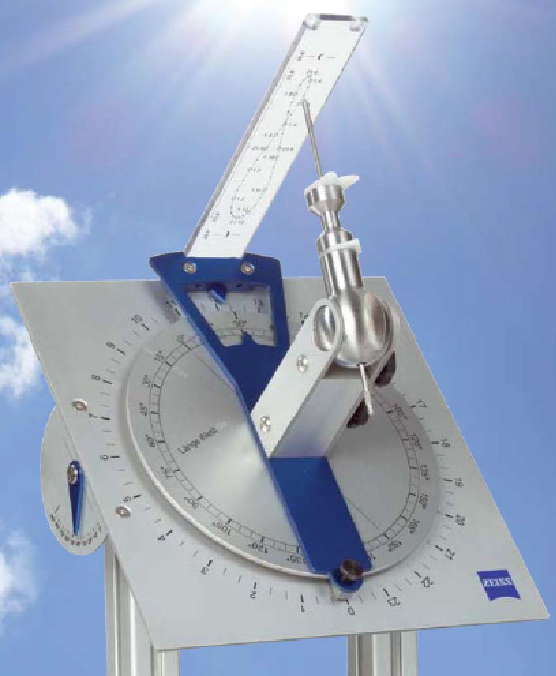
\includegraphics[width=0.5\textwidth]{ZusatzUebung2.pdf}%
\caption{Aalener Sonnenuhr nach Hermann Zeuner.}%
\label{abb:hm_prob_aalener_sonnenuhr}%
\end{figure}

Erl�utern Sie das Grundprinzip und sch�tzen Sie die Genauigkeit ab.
Ist diese Sonnenuhr als Reiseuhr tauglich?\\

\end{prob}
\medskip 
\noindent\rule[1ex]{\textwidth}{0.5pt}

%-----------------------------------------------------------------------------------------------------------
\newpage
\begin{prob} %Zusatz3
\zusatz{hm_Zusatz_VenusTransit_Vorwaerts}{Venustransit 2004 -- Berechnung der Projektion vor der Sonne}
Sehr instruktiv ist eine "`Vorw�rtsrechnung"' des Venustransits, d.h. eine Berechnung der relativen geozentrisch-�quatorialen Koordinaten von Sonne und Venus oder der entsprechenden topographisch-horizontalen Koordinaten (Achtung: hier wirklich topographische Koordinaten verwenden!) mit den heute verf�gbaren Daten aus der St�rungsrechnung.
Hier kann man ebenfalls eine Absch�tzung treffen f�r die notwendige Genauigkeit der Messung der Transitzeiten. F�r die konkrete Kalkulation seien im Folgenden die verwendeten Parameter gegeben:
\begin{align*}
	\frac{D_\text{\astrosun}}{2} &= \sin \lk \frac{31'\,31''}{2} \rk ~, ~~~~
	R_\text{I} = \tan \lk \frac{59''}{2} \rk ~,~~~~
	\hat{R} = \frac{D_\text{\astrosun}}{2} - R_\text{I} ~.
	\end{align*}
\end{prob}
\medskip 
\noindent\rule[1ex]{\textwidth}{0.5pt}

%-----------------------------------------------------------------------------------------------------------

\begin{prob} %Zusatz4
\zusatz{hm_Zusatz_ErdeTransit_from_Mars}{Marsmission 2084 -- Erdtransit vor der Sonne}
Mit zuk�nftigen Marsmissionen wird man nicht bis zum n�chsten Venustransit warten m�ssen, um wieder einen Planeten vor der Sonne vor�berziehen zu sehen.
Ein Beobachter auf dem Mars kann nat�rlich auch beobachten, wie unsere Erde und eventuell ihr Mond vor der Sonne vor�berziehen.
Das letzte Ereignis dieser Art war am 11. Mai 1984 und das n�chste ist am 10.~November 2084 (Wir sind nicht sicher, ob bereits jetzt Anmeldungen entgegen genommen werden.).
Wir empfehlen aber in jedem Fall mit dem \mscr{} \mlhmref{InnerePlaneten.m} das Datum zu �berpr�fen.
F�r eine genauere Rechnung der Transitzeiten benutzen Sie die Koordinatenberechnungen nach der St�rungstheorie, d.h. die Funktionen \mlhmiref{SonneExakt.m}, \mlhmiref{MarsExakt.m}. Wird der Mond gemeinsam mit der Erde vor der Sonne vor�berziehen? \\
\end{prob}
\medskip 
\noindent\rule[1ex]{\textwidth}{0.5pt}


%-----------------------------------------------------------------------------------------------------------
\hypertarget{prb:hm_Z7Praezession}{} %Zusatz5
\begin{prob} %Zusatz6
\zusatz{hm_Zusatz_Praezession}{Berechnung des Drehmomentes f�r die Pr�zession der Erdachse}
Berechnen Sie das Drehmoment der Pr�zession f�r ein Rotationsellipsoid im Gravitationsfeld von Sonne und Mond �ber eine Entwicklung seines Gravitationspotentials nach Kugelfl�chenfunktionen.

\medskip
\noindent\rule[1ex]{\textwidth}{0.5pt}
\end{prob}


%-----------------------------------------------------------------------------------------------------------
\textbf{}
\begin{prob} %Zusatz6
\zusatz{hm_gezeiten08}{L�sung Bewegungsgleichung f�r die Gezeitenreibung}
L�sen Sie das DGL-System \eqref{eq:hm_gezreibung17} numerisch in \matlab{}. 
Gehen Sie dabei wie folgt vor:
\begin{enumerate}
	\item Berechnen Sie das ZKP mit Erde und Mond als Massepunkte um die Stabilit�t ihres numerischen Verfahrens zu testen. Verkleinern Sie eventuell die Schrittweite der Integration. Nutzen Sie \zb \odevf\ oder programmieren Sie selbst eine Euler-Integration.
	\item Gehen Sie dann in das Schwerpunktsystem und wiederholen die Rechnungen und Tests.
	\item Berechnen das ZKP mit Gezeiten. Dazu benutzen Sie \ddezd, einen \matlab-Solver f�r sogenannte DDEs (\textit{Delayed Differential Equations}) oder \textit{retardierte Differentialgleichungen}. Diese sind Differentialgleichungen mit einem nacheilendem Argument, \dh die Ableitung einer gesuchten Funktion $Y(t)$ zum Zeitpunkt $t$ h�ngt nicht nur vom Funktionswert an diesem Zeitpunkt ab, sondern auch von Funktionswerten an fr�heren Zeitpunkten $t-\tau$ oder von Integralen �ber die Funktion �ber vergangene Zeitintervalle. In unserem Fall nehmen wir den Gezeitenberg mit einem festen Delay $\delta = \text{const}$ an. Das gilt dann nat�rlich nur f�r begrenzte Zeiten, hat aber den Vorteil, dass wir die eingebaute \matlab-Routine \ddezd\ f�r das entstehende DDE-DGL-Systeme verwenden k�nnen. Zeigen Sie im Ergebnis der Rechnungen die Inkonsistenz der L�sung auf.
	\item Im n�chsten Schritt n�hern Sie das Delay $\delta$ durch eine lineare Funktion  $\delta(t) = \delta(t=0) \lk(1 - \,\frac{\dot{\omega}_\text{E}}{\omega_\text{E}}\,t\rk $ an, um die Inkonsistenz zu "`heilen"'.  Die Verschiebung des Gezeitenbergs $\delta(t)$ wird langsam gegen Null gehen.
	\item Jetzt lassen wir alle N�herungen fallen, \dh alle Gr��en, auch $\delta(t)$, werden numerisch aus dem DGL-System \eqref{eq:hm_gezreibung17} mit \ddezd\ (Schwerpunktkoordinaten) berechnet. 
	Eine detaillierte Darstellung zur Numerik findet sich \ua in \cite{Schebesta1994}.
\end{enumerate}

\medskip 
\noindent\rule[1ex]{\textwidth}{0.5pt}
\end{prob}

%-----------------------------------------------------------------------------------------------------------

\begin{prob} %Zusatz7
\zusatz{hm_gezeiten_zusatz}{Verbessertes Modell der Gezeitenverformung der Erde.}
Berechnen Sie mit einem verbesserten Modell die Ausformung des Gezeitenellipsoids auf der Erde.
Benutzen Sie die Literatur \cite{Murray2008, Norsen2017}. \\

\medskip 
\noindent\rule[1ex]{\textwidth}{0.5pt}

\end{prob}

%-----------------------------------------------------------------------------------------------------------

\begin{prob} %Zusatz8
\zusatz{hm_pluto_charon}{Pluto-Charon-Liebe.}
Bestimmen Sie aus der heutigen Rotationszeit des Zweik�rper-Systems Pluto-Charon, deren Massen und deren Abstand $d$ die Energie und den Drehimpuls des Systems. Wenn man mal davon ausgeht, dass die beiden Zwergplaneten sich mal eng umschlunegn ahtten, vor wie langer Zeit haben sie sich denn dann getrennt, um die heutige Abstandsposition einzunehmen.\\

\medskip 
\noindent\rule[1ex]{\textwidth}{0.5pt}

\end{prob}

 
%\section {L�sungsbeispiele \autoref{chap:hm} -- Himmelsmechanik}\label{chap:hm_lsguebungen}

Die in den L�sungsvorschl�gen angegebenen \mscre finden sich im GitHub unter \githubSN \bzw
in den \onlineZ{} (\MKc).\\
Sie sind wirklich als Vorschlag f�r eine m�gliche L�sung gedacht, wohl wissend, dass es in der Physik oft ganz verschiedene, manchmal auch elegantere als die hier vorgestellten L�sungen gibt, um ein Problem zu l�sen. Das macht ja gerade den Reiz der Physik aus.
Wir laden die Leser ein, ihre L�sungen auch unter \githubSN \bzw auf den online-Seiten (\MKc) zu teilen.
Wir sind in jedem Fall gespannt.
%%%-----------------------------------------------------------------------------------------------------------

\subsection{�bungen zu Raum und Zeit in der Himmelsmechanik}

\medskip

%-----------------------------------------------------------------------------------------------------------

\begin{sol}{prob:hm_trafo_koord}\label{lsg:hm_trafo_koord} %�bung1
\textbf{Transformation astronomischer Koordinatensysteme} \\
\begin{enumerate}[(a)]
	\item Wie im Kapitel \ref{kap:hm_koordinatensysteme} erl�utert, wird die Transformation von kartesischen Koordinaten aus einem KOS in ein anderes durch Rotationsmatrizen der Form $\mathbb{R}_{x,y,z}(\xi)$ mit dem Drehwinkel $\xi$ und/oder Translationsvektoren beschrieben.
          Man kann sich diese durch geometrische Betrachtungen einfach ableiten.
          Wir geben die Matrizen im Folgenden an und verweisen darauf, dass die R�cktransformation bei Rotationen durch eine Drehmatrix mit dem Winkel $-\xi$ beschrieben wird, die dann wegen der Unitarit�t auf die transponierte Drehmatrix $\lk \mathbb{R}_{x,y,z}(\xi) \rk^\text{T}$ f�hrt.
Wir beschreiben das Vorgehen beispielhaft f�r einige ausgew�hlten Transformationen (siehe auch Beispiel \ref{bsp:herleitung_gauss_vek}):
\begin{itemize}
	\item \emph{Bahn (BA) -- Heliozentrisch-ekliptikal (HE):}
	\begin{align*}
	\mathbb{R}_1 &= \mathbb{R}_z(-\omega) = \lk
	      \begin{matrix} +\cos \omega &\; -\sin \omega &\; 0 \\
	                     +\sin \omega &\; +\cos \omega &\; 0 \\
                          0         &\;     0        &\; 1 
				\end{matrix} \rk  ~~,\\ 
	\mathbb{R}_2 &= \mathbb{R}_x(-i) = \lk
	      \begin{matrix} 1       &\; 0           &\; 0 \\ 
				               0       &\; +\cos i     &\; -\sin i \\ 
											 0       &\; +\sin i     &\; +\cos i 
				\end{matrix} \rk  ~~,\\
	\mathbb{R}_3 &= \mathbb{R}_z(-\Omega) = \lk
	    \begin{matrix} 
	            +\cos \Omega &\; -\sin \Omega &\; 0 \\
	            +\sin \Omega &\; +\cos \Omega &\; 0 \\
                 0         &\;     0        &\; 1 
			 \end{matrix} \rk ~~. 
	\end{align*}
	Die Gesamttransformation wird dann auch mit einer Matrix $\mathbb{U}(-\omega,-i,-\Omega)\!=\! \mathbb{R}_3 \mathbb{R}_2\mathbb{R}_1$ beschrieben.
        Durch Multiplizieren von $\mathbb{U}$ mit dem kartesischen Ausgangsvektor erhalten wir dann die kartesischen heliozentrischen Koordinaten
	\begin{align*}
	r\lk\begin{matrix} \cos b \cos l\\ \cos b \sin l\\ \sin b \end{matrix} \rk = \mathbb{U} \cdot r \lk\begin{matrix} \cos u \\ \sin u \\ 0 \end{matrix} \rk ~~,
	\end{align*}
	aus denen wir dann heliozentrisch die ekliptikalen Parameter $b,l,r$ ableiten k�nnen.\\
	\item \emph{Geozentrisch-ekliptikal (GE)- Geozentrisch-�quatorial (GA):}
		\begin{align*}
	\mathbb{R}_1 &= \mathbb{R}_x(-\epsilon) = \lk
	      \begin{matrix} 1       &\; 0           &\; 0 \\ 
				               0       &\; +\cos \epsilon     &\; -\sin \epsilon \\ 
											 0       &\; +\sin \epsilon     &\; +\cos \epsilon
				\end{matrix} \rk ~~. 
	\end{align*}
	Hier besteht die Transformation nur aus einer Matrix $\mathbb{U}(-\epsilon)\!=\! \mathbb{R}_1$.
        Durch Multiplizieren von $\mathbb{U}$ mit dem kartesischen (GE) Ausgangsvektor erhalten wir dann die kartesischen �quatorialen Koordinaten
	\begin{align*}
	r\lk\begin{matrix} \cos \delta \cos \alpha\\ \cos \delta \sin \alpha\\ \sin \delta \end{matrix} \rk =\mathbb{U} \cdot r \lk \begin{matrix} \cos b \cos l \\ \cos b \sin l \\ \sin l \end{matrix} \rk ~~,
	\end{align*}
	aus denen wir dann die geozentrisch-�quatorialen Koordinaten $\alpha,\delta$ ableiten k�nnen.
\end{itemize}
	\item Wir empfehlen zum Nachvollziehen der Navigationsmethoden fr�herer Jahre die ausf�hrlichen Darstellungen in \cite{Smart1986} und \cite{Weyer2012}.
\end{enumerate}

Wir vergleichen jetzt noch die Bahnparameter der Himmelsmechanik mit den Euler Winkeln\index{Euler-Winkel}, die wir in der Theorie des starren K�rpers (Band I) eingef�hrt hatten.
\begin{table}[h!]
    \centering
    \begin{tabular}{ll}
        \centering Euler-Winkel & Bahnparameter\\
        & \\
         1. Drehung um $\vec{e}_z$-Achse mit Winkel $\varphi$ 
         & 
         1. Drehung um $\vec{e}_z$-Achse mit Winkel $\Omega$ \\
         ~~~~$\mathbb{R}_z\lk\varphi\rk = 
         \begin{pmatrix}
         \cos\varphi & \sin\varphi & 0\\
         -\sin\varphi & \cos\varphi & 0\\
         0 & 0 & 1
         \end{pmatrix}$
         &
          ~~~~$\mathbb{R}_z\lk\Omega\rk  = 
         \begin{pmatrix}
         \cos\Omega & \sin\Omega & 0\\
         -\Omega\varphi & \cos\Omega & 0\\
         0 & 0 & 1
         \end{pmatrix}$\\
         &\\
         2. Drehung um Knotenlinie $\vec{e}_x{}'$ mit Winkel $\vartheta$ &
         2. Drehung um Knotenlinie $\vec{e}_x{}'$ mit Winkel i \\
        ~~~~$\mathbb{R}_x{}'\lk\vartheta\rk = 
         \begin{pmatrix}
         1 & 0 & 0 \\
         0 & \cos\vartheta & \sin\vartheta \\
         0 & -\sin\vartheta & \cos\vartheta
         \end{pmatrix}$ &
         ~~~~$\mathbb{R}_x{}'\lk i\rk = 
         \begin{pmatrix}
         1 & 0 & 0 \\
         0 & \cos i & \sin i \\
         0 & -\sin i & \cos i
         \end{pmatrix}$ \\
         & \\
         3. Drehung um $\vec{e}_z{}''$ mit Winkel $\psi$ & 
         3. Drehung um $\vec{e}_z{}''$ mit Winkel $\omega$ \\
         ~~~~$\mathbb{R}_z{}''\lk\psi\rk = 
         \begin{pmatrix}
         \cos\psi & \sin\psi & 0 \\
         -\sin\psi & \cos\psi & 0 \\
         0 & 0 & 1
         \end{pmatrix}$ &
          ~~~~$\mathbb{R}_z{}''\lk\omega\rk = 
         \begin{pmatrix}
         \cos\omega & \sin\omega & 0 \\
         -\sin\omega& \cos\omega & 0 \\
         0 & 0 & 1
         \end{pmatrix}$ 
    \end{tabular}
\end{table}\\
Wir sehen also, dass die Bahnparameter $\Omega, i, \omega$ den Euler-Winkeln entsprechen.

\end{sol}
\textcolor{blue} {$\rightarrow$ zur} \probref{hm_trafo_koord}.\\
\noindent\rule[1ex]{\textwidth}{0.5pt} \newpage \newpage

%-----------------------------------------------------------------------------------------------------------

\begin{sol}{prob:hm_erdrotation}\label{lsg:hm_erdrotation} %�bung2
\textbf{Verlangsamung der Erdrotation} \\ \\
Wenn man in die Formel \eqref{eq:hm_ueb_verl_erdrot} die Werte
\begin{align*}
a_\text{trop}&=365.2421988 ~, \\
n_\text{Tage}&\approx (2000+135)\cdot 365.25 \approx 779702 \:\text{d}\  \text{bzw. genauer}\\
n_\text{Tage}&=\text{J}2000 - \text{J}(15.04.136 \;\text{v.Chr.})\approx 779691 \:\text{d}
\end{align*}
einsetzt, erh�lt man f�r $\Delta T_\text{rot}\!\approx\!3.7\:\text{h}.$
Das ist recht beachtlich!
Daraus w�rde, wenn man die Sonnenfinsternis nicht mit der Ephemeridenzeit, sondern der um $\Delta T_\text{rot}\!=\!-3.7\:\text{h}$ verschobenen UT berechnet, die Sonnenfinsternis um $\Delta \lambda\!\approx\!55.5\degree$ weiter westlich stattgefunden haben.
Sie wurde aber in Babylon beobachtet.
Wenn man daher den berechneten Wert von $\Delta T_\text{rot}$ in Sekunden ($13300 \:\text{s}$) in die \figref{hm_rotgeschw_sonnenfinsternis} eintr�gt, sieht man eine gute �bereinstimmung mit den beobachteten Daten (siehe auch \cite{Stephenson2016,Steele1997}) und die \href{https://eclipse.gsfc.nasa.gov/SEsearch/SEsearchmap.php?Ecl=-1350415}{NASA Eclipse Web Site}. \\
Man kann sich jetzt noch die Frage stellen, ob man f�r die Verlangsamung der Erdrotation, die im Wesentlichen mit der Gezeitenreibung (siehe \kap{hm_gezeitenreibung}) erkl�rt wird, eine einfache Absch�tzung findet.
Wir betrachten dazu das Erde-Mond-System und vernachl�ssigen den Einfluss der Sonne.
Ferner nehmen wir der Einfachheit halber eine Bahnebene f�r Mond und Erde an und vernachl�ssigen auch die Polneigung der Erde.
F�r dieses System gilt Drehimpulserhaltung, der Gesamtdrehimpuls setzt sich dabei wie folgt zusammen:
\begin{figure}[H]
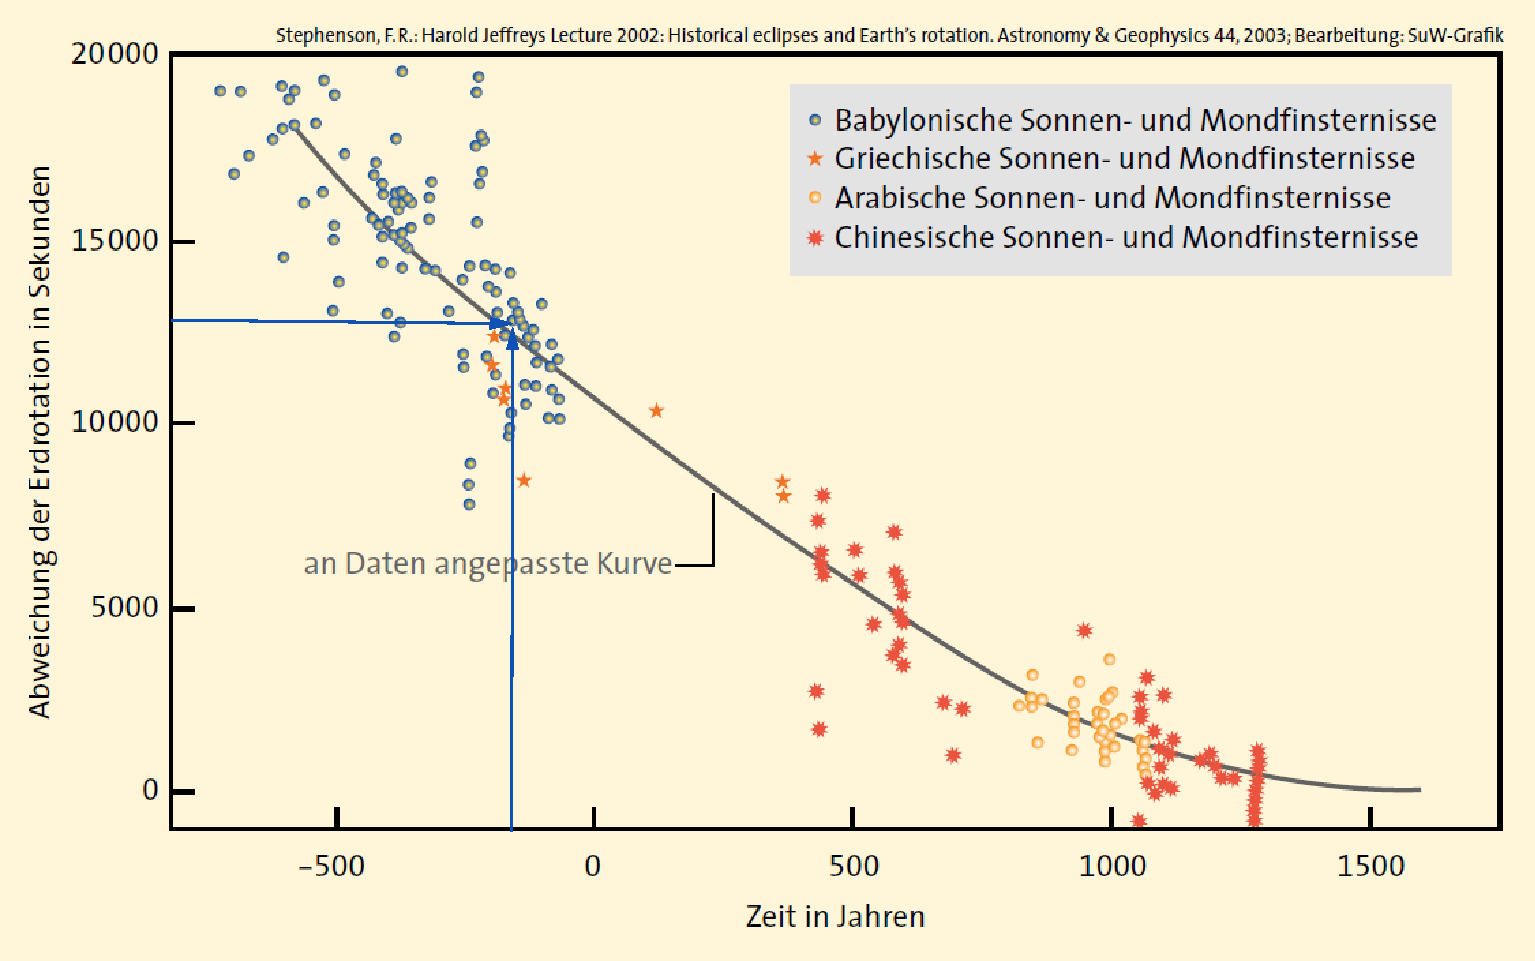
\includegraphics[width=\columnwidth]{SofiHistory.pdf}%
\caption[Abnahme der Rotationsgeschwindigkeit der Erde.]{Abnahme der Rotationsgeschwindigkeit der Erde aus Beobachtung von Sonnenfinsternissen \cite{Stephenson2016,Bastian2020}}%
\label{abb:hm_rotgeschw_sonnenfinsternis}% 
\end{figure}  
\begin{align*}
		\vec{L}_g =\sum \vec{L}_i = \vec{const} = \vec{L}_{\earth,\text{Rotation}} + \vec{L}_{\earth \text{/Mond},\text{Bahn}} + \vec{L}_\text{Mond, Rotation}  ~~.
\end{align*}
Die einzelnen Terme sind der Eigendrehimpuls der Erde, der Bahndrehimpuls des Mondes um die Erde und Eigendrehimpuls des Mondes, wobei wir letzteren auf Grund der Massenverh�ltnisse und der langsamen Rotation vernachl�ssigen k�nnen.
Eine Reduktion der Eigenrotations-Geschwindigkeit der Erde muss dann also zu einem Anwachsen des Bahndrehimpulses f�hren.
Da wir das Problem in einer Ebene behandeln wollen, k�nnen wir zu skalaren Gr��en �bergehen.
Der Betrag des Eigendrehimpulses der Erde ist dann gegeben durch $L_{\earth,\text{Rotation}} = J_{\earth} \omega_{\earth}$, der Bahndrehimpulsbetrag durch $L_{\earth \text{/Mond},\text{Bahn}} = m_{\text{M}} a_{\earth \text{M}} ^2 \omega_{\earth \text{M}}$.
Der Endzustand nach langer Zeit ($t \rightarrow \infty$) ist dann erreicht, wenn $ \omega_{\earth , \infty} = \omega_{\earth \text{M}, \infty}$, d.\,h. die Erde rotiert dann genau so schnell um sich, wie der Mond um die Erde.\\
Wir multiplizieren das Tr�gheitsmoment der Erde mit einem Faktor von $3/4$, da wir den Kern als dichter als den �u�eren Teil der Erdkruste annehmen, d.\,h. $		J_{\earth} = 0.75 \, \frac{2}{5} m_{\earth} R_{\earth}^2 $.
Mit den heutigen Werten f�r $m_{\earth}, m_{\text{M}}, a_{\earth \text{M}}, \omega_{\earth}$, und $\omega_{\earth {\text{M}}}$ kann man den Gesamtdrehimpuls berechnen zu:
	\begin{align*}
	L_g = \frac{3}{4} \, \frac{2}{5} \,m_{\earth} \,R_{\earth}^2 \, \omega_{\earth} + m_{\text{M}}\, a_{\earth \text{M}} ^2 \, \omega_{\earth \text{M}} \approx 3.4 \cdot 10^{34} \;\text{kg}\,\text{m}^2\,\text{s}^{-1} ~.
	\end{align*}
Da heute schon der Bahndrehimpuls bedeutend gr��er als der Eigendrehimpuls der Erde ist (Faktor $5$), wird das erst recht im Zustand der gebundenen Rotation gelten.
Wir k�nnen also schreiben:
	\begin{align}
	L_{g,\infty} \approx L_{\earth \text{M},\infty} = m_{\text{M}} \,  a_{\earth \text{M}, \infty} ^2 \, \omega_{\earth \text{M}, \infty} ~.\label{eq:hm_lsg_lges_inf}
	\end{align}
Andererseits gilt in guter N�herung das dritte Keplersche Gesetz, das wir mit $T_i=2\pi/\omega_i$ schreiben als:
	\begin{align}
	\omega_{\earth \text{M}, \infty} ^2 \, a_{\earth \text{M}, \infty} ^3 = \omega_{\earth \text{M}} ^2 \, a_{\earth \text{M}} ^3 ~.\label{eq:hm_lsg_kep3}
	\end{align}
Wir haben damit zwei Gleichungen f�r zwei Unbekannte ($\omega_{\earth \text{M}, \infty}$ und $a_{\earth \text{M}, \infty}$).
Aufgel�st ergeben diese
	\begin{align}
\omega_{\earth \text{M}, \infty} &= \omega_{\earth, \infty} \approx \frac{\omega_{\earth}^4 \, a_{\earth \text{M}} ^4 \, m_{\text{M}} ^3 }{L_g^2} \;\Rightarrow\:\frac{T_{\earth, \infty}}{T_{\earth}} \!=\!\lk \frac{\omega_{\earth, \infty}}{\omega_{\earth}} \rk ^{-1} \approx 45.3 ~,\label{eq:hm_lsg_finale_omega} \\ 
	a_{\earth \text{M}, \infty} &= \frac{L_g^2}{\omega_{\earth \text{M}}^2 \, a_{\earth \text{M}}^3 \, m_{\text{M}}^2} \; \Rightarrow\:\frac{a_{\earth \text{M}, \infty}}{a_{\earth \text{M}}} \approx 1.4 ~.\label{eq:hm_lsg_finale_abst}
	\end{align}
	Unser Erdentag wird damit zu dem Zeitpunkt der gebundenen Rotation etwa 45 mal so lang sein \eqref{eq:hm_lsg_finale_omega}, was uns eine ausgedehnte Nachtruhe verschaffen wird.
        Auf der anderen Seite wird es zwar weiterhin Sonnenbedeckungen durch den Mond geben, allerdings wegen \eqref{eq:hm_lsg_finale_abst} keine Totalfinsternisse mehr, \ldots was sehr schade ist.
        Wann es so weit sein wird, kann man ja mal unter Annahme der G�ltigkeit der Formel \eqref{eq:hm_ueb_verl_erdrot} f�r die Erdabbremsung nachrechnen.
        Wir wollten es eiegntlich gar nicht so genau wissen. Weitere Rechnungen zur Gezeitenreibung finden sich in \kap{hm_gezeitenreibung} und \probref{hm_gezeiten07}. \\
				
\end{sol}
\textcolor{blue} {$\rightarrow$ zur} \probref{hm_erdrotation}.\\
\noindent\rule[1ex]{\textwidth}{0.5pt} \newpage \newpage

%-----------------------------------------------------------------------------------------------------------

\begin{sol}{prob:hm_sideric_period_mars}\label{lsg:hm_sideric_period_mars} %�bung3
\textbf{Siderische Umlaufzeit des Mars} \\ \\
Wir benutzen die Geometrie aus \figref{hm_sideric_period_mars} und betrachten den Winkel (die heliozentrische L�ngen, die zwischen zwei Mars-Oppositionen �berstrichen wird.
Dies entspricht der messbaren synodischen Umlaufzeit $T_{\text{syn},\mars}$ des Mars.
Wir vernachl�ssigen bei unserer Betrachtung die Exzentrizit�t\footnote{Eine sch�ne Anleitung f�r die eigene Beobachtung der elliptischen Bahn des Mars und deren Ber�cksichtigung bei der Berechnung der siderischen Umlaufzeit findet sich in \cite{Krisciunas2019}.} und auch die relative Neigung der beiden Planetenbahnen.
Da die synodische Umlaufzeit des Mars gr��er als ein Erdjahr ist, ist die Winkelgeschwindigkeit $\omega_{\mars}$ des Mars kleiner ist als die der Erde $\omega_{\earth}$.
Mit den siderischen Umlaufzeiten $T_{\earth}$ und $T_{\mars}$ ergeben sich dann folgende �berstrichene Winkel (heliozentrische L�ngen) f�r die Zeit zwischen den beiden Oppositionen.
\begin{align*}
	T_{\mars} = \frac{2\pi\degree}{\omega_{\mars}} ~~\longrightarrow \;l_{\mars} = T_{\text{syn},\mars}\,\omega_{\mars} ~~\text{und} ~~
	T_{\earth} = \frac{2\pi\degree}{\omega_{\earth}} ~~\longrightarrow \;l_{\earth} = T_{\text{syn},\mars}\,\omega_{\earth} ~~. \end{align*}
\begin{figure}[H]
\centering
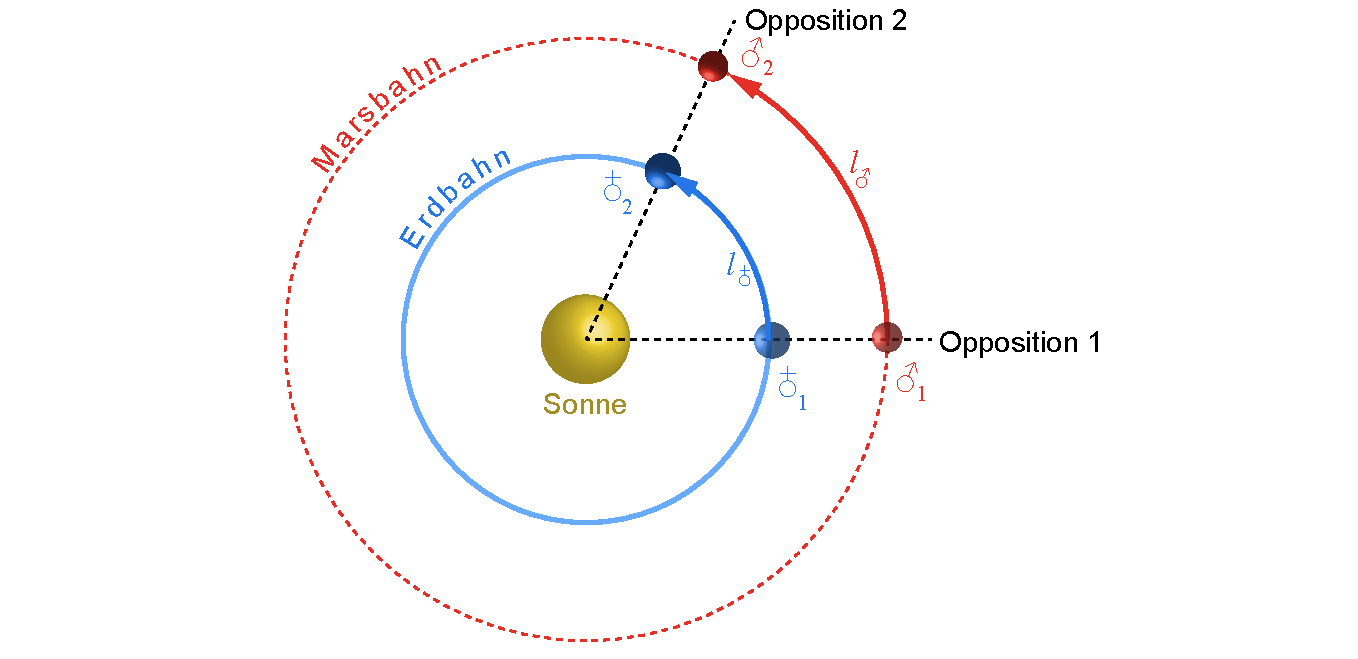
\includegraphics[width=0.9\columnwidth]{Mars_Erde_Umlauf.pdf}%
\caption{Zur Berechnung der siderischen Umlaufzeit des Mars}%
\label{abb:hm_sideric_period_mars}%
\end{figure}
Die Differenz beider L�ngen muss aber wieder $2\pi$ sein.
Daher gilt
\begin{equation*}
	\Delta l= l_{\earth} - l_{\mars} = 2\pi = T_{\text{syn},\mars} \,\lk \omega_{\earth} - \omega_{\mars}\rk = T_{\text{syn},\mars}\, 2\pi\, \lk\frac{1}{T_{\earth}}-\frac{1}{T_{\mars}}\rk ~, 
\end{equation*}
woraus mit $T_{\text{syn},\mars}\!\approx\!779.94\:\text{d}$ und $T_{\earth}\!\approx\!365.256\:\text{d}$ folgt:
\begin{align*}
T_{\mars} = \frac{{T_{\text{syn},\mars}}\, T_{\earth}}{T_{\text{syn},\mars} - T_{\earth}} = 686.980\:\text{d} ~~.\\
\end{align*}
\end{sol}
\textcolor{blue} {$\rightarrow$ zur} \probref{hm_sideric_period_mars}.\\
\noindent\rule[1ex]{\textwidth}{0.5pt} \newpage


%%%-----------------------------------------------------------------------------------------------------------

\subsection{�bungen zur Kepler-Gleichung}

\medskip

%-----------------------------------------------------------------------------------------------------------

\begin{sol}{prob:hm_laplace}\label{lsg:hm_laplace} %�bung4
\textbf{Laplace-Integral} \\
\begin{enumerate}[(i)]
	\item Wir starten von 
\begin{align*}
\vec{L} \times \ddot{\vec{r}} &= \lk \vec{r} \times \dot{\vec{r}}\rk \times \lk \frac{-\mu_\text{G}}{r^3} \rk\, \vec{r} \\
															&= \frac{\mu_\text{G}}{r^3}\,\vec{r}\times \lk \vec{r} \times \dot{\vec{r}}\rk
\end{align*}
Mit der Vektoralgebra-Beziehung 
\begin{equation*}
\vec{a}\times(\vec{b}\times\vec{c}) = \vec{b}(\vec{a}\cdot\vec{c}) - \vec{c}(\vec{a}\cdot\vec{b}) ~~.
\end{equation*}
folgt
\begin{align*}
\vec{L} \times \ddot{\vec{r}} &= \frac{\mu_\text{G}}{r^3} \lek \vec{r}(\vec{r}\cdot\dot{\vec{r}})-\dot{\vec{r}}(\vec{r}\cdot\vec{r}) \rek \\
															&= \frac{\mu_\text{G}}{r^3} \lek \vec{r}(\vec{r}\cdot\dot{\vec{r}})-\dot{\vec{r}}\,r^2\rek  ~.
\end{align*}
In Polarkoordinaten geschrieben ($\vec{r}=r\vec{e}_r$, $\dot{\vec{r}}=\dot{r}\vec{e}_r + r\dot{\vartheta}\vec{e}_\vartheta$) und wegen $\vec{e}_r\!\perp\!\vec{e}_\vartheta$ wird daraus
\begin{align}
\vec{L} \times \ddot{\vec{r}} &= \frac{\mu_\text{G}}{r^3} \lek \vec{r}(r\cdot \dot{r}) - \dot{\vec{r}}(r^2)\rek \nonumber\\
															&= \frac{\mu_\text{G}}{r^2} \dot{r}\,\vec{r} - \frac{\mu_\text{G}}{r}\,\dot{\vec{r}} = -\frac{\D}{\D t} \lk \frac{\mu_\text{G}}{r} \,\vec{r} \rk ~~.\label{eq:hm_laplace_lsg1} 
\end{align}
Die linke Seite kann wegen $\vec{L}\!=\!\vec{const}$ als Zeitableitung geschrieben werden:
\begin{equation*}
\vec{L} \times \ddot{\vec{r}} = \frac{\D }{\D t} \lk \vec{L} \times \dot{\vec{r}}\rk ~~,
\end{equation*}
woraus wir mit \eqref{eq:hm_laplace_lsg1}
\begin{align*}
\frac{\D }{\D t} \lk \vec{L}\times\dot{\vec{r}} + \frac{\mu_\text{G}}{r}\,\vec{r}\rk &= 0 
\end{align*}
erhalten.
Integration mit $-\mu_\text{G}\,\vec{e}$ als Integrationskonstante ergibt
\begin{align*}
\vec{L}\times\dot{\vec{r}} + \frac{\mu_\text{G}}{r}\,\vec{r} &= \vec{const} = -\mu_\text{G} \vec{e}
\end{align*}
und damit schlussendlich
\begin{align}
\vec{e} &= -\frac{1}{\mu_\text{G}} \lk \vec{L}\times\dot{\vec{r}} + \frac{\mu_\text{G}}{r}\,\vec{r} \rk  ~~. \label{eq:hm_laplace_lsg2}
\end{align}
\medskip
\item Wir zeigen nun, dass 
\begin{equation*}
\mu_\text{G}^2(e^2-1) = 2HL^2 ~~.
\end{equation*}
Dazu bilden wir ausgehend von \eqref{eq:hm_laplace_lsg2} das Betragsquadrat:
\begin{align*}
\lk -\mu_\text{G} \vec{e} \rk^2 &= \lk \vec{L}\times\dot{\vec{r}} + \frac{\mu_\text{G}}{r}\,\vec{r} \rk^2 \\
\Rightarrow \mu_\text{G}^2e^2 &= \lk \vec{L}\times\dot{\vec{r}} \rk^2 + \frac{2\mu_\text{G}}{r}\,\vec{r} \lk \vec{L}\times\dot{\vec{r}} \rk + \frac{\mu_\text{G}^2}{r^2}\,\vec{r}^2 \\
															&= \lek (\vec{r}\times\dot{\vec{r}})\times\dot{\vec{r}} \rek^2 + \frac{2\mu_\text{G}}{r}\,\vec{r} \lk \vec{L}\times\dot{\vec{r}} \rk + \mu_\text{G}^2 \\
															&= [\underbrace{(\vec{r}\cdot\dot{\vec{r}})\dot{\vec{r}}}_{0} - \underbrace{(\dot{\vec{r}}\cdot\dot{\vec{r}})}_{\dot{r}^2=v^2}\vec{r}]^2 + \frac{2\mu_\text{G}}{r}\,\vec{r} \lek (\vec{r}\times\dot{\vec{r}})\times\dot{\vec{r}} \rek + \mu_\text{G}^2\\
															&= v^4 r^2 + \frac{2\mu_\text{G}}{r}\,\vec{r} [ (\underbrace{\vec{r}\cdot\dot{\vec{r}})\dot{\vec{r}}}_{0} - \dot{\vec{r}}^2\vec{r} ] + \mu_\text{G}^2 \nonumber \\ 
															&= v^4 r^2 - \frac{2\mu_\text{G}}{r}\,v^2 r^2 + \mu_\text{G}^2 \nonumber 
\end{align*}															
\begin{align}													
\Rightarrow \mu_\text{G}^2 \lk e^2-1\rk &= v^4 r^2 - 2 \mu_\text{G} v^2 r ~~. \label{eq:hm_laplace_lsg3}
\end{align}
Wir benutzen jetzt die Definition $2 H\!\equiv\!v^2-(2\mu_\text{G}/r)$ und $L\!=\!\abs{\vec{L}}\!=\!\abs{\vec{r}\times \vec{v}}\!=\! rv$ und erhalten als Zwischenergebnis
\begin{align*}
2HL^2 = \underbrace{\lk v^2 - \frac{2\mu_\text{G}}{r}\rk}_{2 H} \underbrace{\lk r^2 v^2\rk}_{L^2} = v^4r^2 - 2\mu_\text{G}v^2 r ~~.
\end{align*}
was wir in \eqref{eq:hm_laplace_lsg3} einsetzen, woraus schlie�lich folgt:
\begin{equation*}
\mu_\text{G}^2 \lk e^2-1\rk  = 2 HL^2~~.
\end{equation*}
\end{enumerate}
\end{sol}
\textcolor{blue} {$\rightarrow$ zur} \probref{hm_laplace}.\\
\noindent\rule[1ex]{\textwidth}{0.5pt} \newpage

%-----------------------------------------------------------------------------------------------------------

\begin{sol}{prob:hm_wahre_anomalie}\label{lsg:hm_wahre_anomalie} %�bung5
\textbf{Wahre Anomalie}\\ \\
Wir starten von der Definition der exzentrischen Anomalie \eqref{eq:hm_exzentrische_Anomalie}:
\begin{equation*}
r(t) = a \lk 1-e\,\cos E\rk 
\end{equation*}
und benutzen dann \figref{hm_geom_abl_kepler}, so dass
\begin{align}
\overline{\text{NZ}} \equiv \overline{x}_\text{P} &= \overline{\text{ON}} - \overline{\text{OZ}} \nonumber\\
																						 &= a\cos E - ae \nonumber\\
																						 &= a (\cos E -e) \nonumber\\
\Rightarrow \cos\upsilon = 	\frac{\overline{x}_\text{P}}{r} &= \frac{\cos E-e}{1-e\cos E} ~~. \label{eq:hm_wa_lsg1}
\end{align}
Zun�chst schreiben wir \eqref{eq:hm_wa_lsg1} um in
\begin{align}
1-\cos \upsilon &= \frac{1-e\cos E - \cos E + e}{1-e\cos E} = \frac{(1+e)(1-\cos E)}{1-e\cos E} ~~, \label{eq:hm_wa_lsg2}\\
1+\cos \upsilon &= \frac{1-e\cos E + \cos E - e}{1-e\cos E} = \frac{(1-e)(1+\cos E)}{1-e\cos E} ~~. \nonumber
\end{align}
Um auf den halben Winkel in \eqref{eq:hm_nu(t)_alternativ} zu kommen, nutzen wir die Winkelfunktionsbeziehungen
\begin{align*}
1-\cos x &= 2\sin^2\lk\frac{x}{2}\rk ~~, \\
1+\cos x &= 2\cos^2\lk\frac{x}{2}\rk ~~ 
\end{align*}
und benutzen diese in \eqref{eq:hm_wa_lsg2}.
Wir erhalten sofort nach Quotientenbildung und Wurzelziehen
\begin{align*}
\lk 1 - e\, \cos E\rk \;2 \sin^2\lk\frac{\upsilon}{2}\rk &= 2(1+e)\sin^2\lk\frac{E}{2}\rk ~~,\\
\lk 1 - e\, \cos E\rk \;2 \cos^2\lk\frac{\upsilon}{2}\rk &= 2(1-e)\cos^2\lk\frac{E}{2}\rk ~~,\\
   \rightarrow~~ \tan\lk\frac{\upsilon}{2}\rk &= \sqrt{\frac{1+e}{1-e}}\,\tan\lk\frac{E}{2}\rk~~.
\end{align*}
\end{sol}
\textcolor{blue} {$\rightarrow$ zur} \probref{hm_wahre_anomalie}.\\
\noindent\rule[1ex]{\textwidth}{0.5pt} \newpage

%-----------------------------------------------------------------------------------------------------------

\begin{sol}{prob:hm_bwglg_hyp_parab}\label{lsg:hm_bwglg_hyp_parab} %�bung6
\textbf{Bewegungsgleichungen f�r Hyperbel und Parabel} \\
\begin{enumerate}[(i)]
	\item \emph{Hyperbel}\\
	Diese Herleitung erfolgt analog zur Kepler-Gleichung f�r die Ellipse.
        Man f�hrt lediglich anstelle der Hilfsgr��e \anf{exzentrische Anomalie} eine \anf{hyperbolische exzentrische Anomalie} $E_\text{hyp}$ ein.
        Man beachte dabei, dass bei einer Hyperbel $a\!<\!0$ ist.
        Zudem ben�tigen wir f�r die weitere Rechnung folgende Beziehungen f�r Hyperbelfunktionen:
\begin{align*}
\sinh^2x &= \cosh^2x-1 ~~, \\
\sinh x &= \frac{\D }{\D x} \cosh x ~~,\\
\cosh x &= \frac{\D }{\D x} \sinh x ~~.
\end{align*}
Wir starten zun�chst mit
\begin{align}
r &= a_\text{hyp} (1-e\cosh E_\text{hyp}) \nonumber \\
  &= \abs{a_\text{hyp}} (e\cosh E_\text{hyp} - 1) \label{eq:hm_hyplsg1} 
\end{align}
und bilden die zeitliche Ableitung, die wir anschlie�end quadrieren:
\begin{align}
\frac{\D r}{\D t} =&\, +\abs{a_\text{hyp}}e \sinh E_\text{hyp}\,\lk\frac{\D E_\text{hyp}}{\D t}\rk  \nonumber \\ 
\lk\frac{\D r}{\D t}\rk^2 =&\, +\, \abs{a_\text{hyp}}^2 e^2 (\sinh E_\text{hyp})^2 \,\lk\frac{\D E_\text{hyp}}{\D t}\rk^2 ~.\label{eq:hm_hyplsg2}
\end{align}
Dann starten wir wieder mit der Bahngeschwindigkeit in Polarkoordinaten und benutzen \eqref{eq:hm_dot_r_quadrat}, so dass
\begin{align*}
\lk\frac{\D r}{\D t}\rk^2 =&\, \frac{\mu_\text{G}}{r^2} \lk 2r-\frac{r^2}{a_\text{hyp}}\rk -\lk \frac{a_\text{hyp}(1-e^2)}{r^2} \rk\,\mu_\text{G} ~~.
\end{align*}
Wir setzen jetzt f�r $r$ die Beziehung \eqref{eq:hm_hyplsg1} ein und erhalten 
\begin{align*}
\lk\frac{\D r}{\D t}\rk^2 =&\, \frac{\mu_\text{G}}{r^2} \lk \killA{2\abs{a_\text{hyp}} e \cosh E_\text{hyp}} - \killB{2 \abs{a_\text{hyp}}} +\frac{\abs{a_\text{hyp}}^2}{\abs{a_\text{hyp}}} e^2 \cosh^2 E_\text{hyp} \right.\\
&\,\left. +\killB{\frac{\abs{a_\text{hyp}}^2}{\abs{a_\text{hyp}}}} - \killA{\frac{2\abs{a_\text{hyp}}^2}{\abs{a_\text{hyp}}}e\cosh E_\text{hyp}} + \killB{\abs{a_\text{hyp}}} -\abs{a_\text{hyp}} e^2\rk \\
=&\, \frac{\mu_\text{G}}{r^2} \lk \abs{a_\text{hyp}} e^2 \cosh^2 E_\text{hyp} - \abs{a_\text{hyp}} e^2\rk \\
=&\, \frac{\mu_\text{G}}{r^2} \abs{a_\text{hyp}} e^2 \underbrace{\lk \cosh^2 E_\text{hyp} - 1\rk}_{\sinh^2 E_\text{hyp}} ~~, 
\end{align*}
und weiter mit \eqref{eq:hm_hyplsg2}
\begin{align*}
\abs{a_\text{hyp}}^{\killA{2}} \killA{e^2 \sinh^2 E_\text{hyp}} \,\lk \frac{\D E_\text{hyp}}{\D t}\rk^2 &= \frac{\mu_\text{G}}{r^2} \killA{\abs{a_\text{hyp}} e^2 \sinh^2 E_\text{hyp}} \\
\Rightarrow r \lk \frac{\D E_\text{hyp}}{\D t}\rk &= \sqrt{\frac{\mu_\text{G}}{\abs{a_\text{hyp}}}} ~~.
\end{align*}
Wir setzen wieder f�r $r$ die Beziehung \eqref{eq:hm_hyplsg1} ein und bekommen
\begin{align*}
\abs{a_\text{hyp}} (e\cosh E_\text{hyp} - 1)\,\D E_\text{hyp} &= \sqrt{\frac{\mu_\text{G}}{\abs{a_\text{hyp}}}} \,\D t ~~,
\end{align*}
woraus nach Integration 
\begin{align}
e \sinh E_\text{hyp} - E_\text{hyp}  &= \sqrt{\frac{\mu_\text{G}}{\abs{a_\text{hyp}}^3}} (t-t_0) = M_\text{hyp}(t-t_0) ~~  \label{eq:hm_hyplsg3}
\end{align}
eine hyperbolische modifizierte Kepler-Gleichung resultiert.
Die L�sung dieser Gleichung erfolgt ebenfalls numerisch durch Iteration oder Reihenentwicklung.\\

\item \emph{Parabel}\\
Bei der Parabel ist die Situation interessanterweise etwas einfacher.
Wir wissen ja, dass f�r die Parabel $e\!=\!1$ ist.
Somit arbeiten wir mit dem Parameter $p$.
Wir starten von der Kegelschnittgleichung \eqref{eq:hm_kegelschnitt}:
\begin{equation*}
r(\upsilon) = \frac{L^2}{\mu_\text{G}}\,\frac{1}{1+\cos \upsilon} = \frac{p}{1+\cos \upsilon} ~~.
\end{equation*}
Andererseits ist noch wegen \eqref{eq:hm_drehimp_z} $L\!=\!r^2\dot{\upsilon}$, so dass wir fortfahren mit
\begin{align*}
\frac{\D \upsilon}{\D t} &= \frac{L}{r^2} \Rightarrow r^4\,\lk\frac{\D \upsilon}{\D t}\rk^2 = L^2 = \mu_\text{G}p \\
\Rightarrow \frac{\D \upsilon}{\D t} &= \sqrt{\mu_\text{G} p} \lk\frac{1}{r^2}\rk = \sqrt{\mu_\text{G} p}\,\lk\frac{(1+\cos\upsilon)^2}{p}\rk^2 \\
\Rightarrow \D \upsilon &= \sqrt{\frac{mu_\text{G}}{p^3}} \lek 2\cos^2\lk\frac{\upsilon}{2}\rk\rek^2 \,\D t ~~,
\end{align*}
wobei wir in der letzten Zeile die Beziehung $1+\cos x\!=\!2\cos^2(x/2)$ verwendet haben.
Damit erhalten wir nach Trennung der Variablen
\begin{equation*}
\frac{1}{2} \lk \,\frac{1}{\cos^4 \lk\frac{\upsilon}{2}\rk} \rk\,\D \lk\frac{\upsilon}{2}\rk  = \sqrt{\frac{\mu_\text{G}}{p^3}}\,\D t ~~.
\end{equation*}
In Integraltabellen findet man $\int (\cos^{-4} u)\,\D u \!=\! \tan u + (1/3)\tan^3 u + c$, was man leicht durch Differenzieren pr�fen kann.
Damit erhalten wir nun eine Bestimmungsgleichung f�r $\upsilon$:
\begin{equation*}
\tan\lk\frac{\upsilon}{2}\rk + \frac{1}{3}\tan^3\lk\frac{\upsilon}{2}\rk = 2 \sqrt{\frac{\mu_\text{G}}{p^3}} (t-t_0)~~.
\end{equation*}
Aus der Parabelgleichung folgt f�r $\upsilon\!=\!0$ die Periheldistanz $q$ zu
\begin{equation*}
q = \frac{p}{1+\cos(0)} = \frac{p}{2}
\end{equation*}
und daraus die sogenannte Barkersche Gleichung f�r die wahre Anomalie der Bahn der Parabel
\begin{equation}
\tan\lk\frac{\upsilon}{2}\rk  + \frac{1}{3} \tan^3\lk\frac{\upsilon}{2}\rk  = \sqrt{\frac{4\mu_\text{G}}{8q^3}} (t-t_0) = \sqrt{\frac{\mu_\text{G}}{2q^3}} (t-t_0)~~.
\label{eq:hm_BarkerGleichung01}
\end{equation}
Das ist noch eine transzendente Gleichung in $\upsilon$.
Setzt man aber $\tan(\upsilon/2)\!=\!u$, so wird daraus
\begin{equation}
u+\frac{1}{3}u^3 = M_\text{P}(t-t_0)~~, \label{eq:hm_BarkerGleichung02}
\end{equation}
gl�cklicherweise eine mit den bekannten Formeln f�r kubische Gleichungen analytisch l�sbare Form.
Mit
\begin{equation*}
A = \frac{3}{2} \sqrt{\frac{\mu_\text{G}}{2q^3}} (t-t_0)A ~~~\text{und}~~~B = \sqrt[3]{A+\sqrt{A^2+1}}
\end{equation*}
findet man:
\begin{equation}
   \upsilon = 2\arctan{(\lk b - \frac{1}{B}\rk }\,. \label{eq:hm_BarkerGleichung03}
\end{equation}

Im Gegensatz zur Ellipse und Hyperbel hat also der Spezialfall der Parabel\index{Parabel} eine geschlossene analytische L�sung.
Wir werden dieser Barkerschen Gleichung\index{Barkersche Gleichung} in modifizierte Form bei der Berechnung von Kometenbahnen wieder begegnen.
\end{enumerate}
\end{sol}
\textcolor{blue} {$\rightarrow$ zur} \probref{hm_bwglg_hyp_parab}.\\
\noindent\rule[1ex]{\textwidth}{0.5pt} \newpage

%-----------------------------------------------------------------------------------------------------------

\begin{sol}{prob:hm_iteration}\label{lsg:hm_iteration} %�bung7
\textbf{Iteration} \\ \\
Die Rechnungen sind im Detail in \mlhmref{KeplerVergleich.m} ausgef�hrt. 
\end{sol}
\textcolor{blue} {$\rightarrow$ zur} \probref{hm_iteration}.\\
\noindent\rule[1ex]{\textwidth}{0.5pt} \newpage

%-----------------------------------------------------------------------------------------------------------

\begin{sol}{prob:hm_bessel}\label{lsg:hm_bessel} %�bung8
\textbf{Bessel-Reihe} \\ \\
Die Rechnungen sind im Detail im \mscr{} \mlhmref{Besselreihe.m} ausgef�hrt. 
\end{sol}
\textcolor{blue} {$\rightarrow$ zur} \probref{hm_bessel}.\\
\noindent\rule[1ex]{\textwidth}{0.5pt} \newpage

%-----------------------------------------------------------------------------------------------------------

\begin{sol}{prob:hm_alternative_MPG}\label{lsg:hm_alternative_MPG} %�bung9
\textbf{Alternative Herleitung der Mittelpunktsgleichung} \\ \\
Im Beispiel \ref{bsp:mittelpktglg} hatten wir die Mittelpunktsgleichung �ber die Bessel-Reihe hergeleitet.
Wir wollen hier nun Herleitung �ber die Iterationsl�sung nach Kapitel \ref{kap:iteration_kepler} wiederholen und folgen dabei der eleganten Darstellung in \cite{Smart1986}. Wir starten mit \eqref{eq:hm_nu(t)_alternativ} (siehe auch \probref{hm_wahre_anomalie}):
\begin{equation*}
\tan \lk \frac{\upsilon}{2} \rk = \sqrt{\frac{1+e}{1-e}}\,\tan\lk\frac{E}{2}\rk ~~.
\end{equation*}
Wir setzen $\sin\alpha\!=\!e$, da $0\!\leq\! e\!\leq\! 1$, was aus $0\!\leq\!\alpha\!\leq\!\pi$ folgt.
Mit der Identit�t 
\begin{align*}
1 \pm \sin\alpha &= 1 \pm \frac{2 \tan\lk\frac{\alpha}{2}\rk}{1+\tan^2\lk\frac{\alpha}{2}\rk} = \frac{1 \pm 2 \tan\lk\frac{\alpha}{2}\rk+\tan^2\lk\frac{\alpha}{2}\rk}{1+\tan^2\lk\frac{\alpha}{2}\rk} \\
                 &= \frac{{\lk 1 \pm \tan\lk\frac{\alpha}{2}\rk \rk}^2}{1+\tan^2\lk\frac{\alpha}{2}\rk}
\end{align*}
erh�lt man
\begin{equation}
\tan \lk \frac{\upsilon}{2} \rk  = \frac{1+\tan\lk\frac{\alpha}{2}\rk}{1-\tan\lk\frac{\alpha}{2}\rk}\,\tan\lk\frac{E}{2}\rk = \frac{1+x}{1-x}\,\tan\lk\frac{E}{2}\rk~~. \label{eq:hm_lsg_mpg_1}
\end{equation}
Wir benutzen nun die Euler-Gleichungen $\cos\theta\!=\!1/2 \lk \E^{\im\theta}+\E^{-\im\theta}\rk$ und $\sin\theta\!=\!1/(2\im)\lk\E^{\im\theta}-\E^{-\im\theta}\rk$ und schreiben mit dem Tangens des halben Winkels $\upsilon$ und analog f�r den Tangens des halben Winkel $E$ die Beziehung f�r die wahre Anomalie als
\begin{equation*}
\tan \lk \frac{\upsilon}{2} \rk = \frac{\E^{+\im\upsilon/2} - \E^{-\im\upsilon/2}}{i\lk\E^{+\im\upsilon/2} + \E^{-\im\upsilon/2}\rk} = \frac{\E^{\im\upsilon}-1}{i\lk \e^{\im\upsilon} + 1\rk} \frac{\killA{\E^{-\im\upsilon/2}}}{\killA{\E^{-\im\upsilon/2}}}~~,
\end{equation*}
woraus mit \eqref{eq:hm_lsg_mpg_1} folgt
\begin{equation}
\frac{\E^{\im\upsilon}-1}{\E^{\im\upsilon}+1} = \frac{1+x}{1-x}\,\frac{\E^{\im E}-1}{\E^{\im E}+1}~~.
\label{eq:hm_lsg_mpg_2}
\end{equation}
Wir setzen nun $\E^{\im\upsilon}\!\equiv\!\E^q$ und die rechte Seite gleich $Q$.
Damit ergibt sich vereinfacht
\begin{align}
\E^q -1 &= Q\lk \E^q+1\rk \nonumber\\
\E^q \lk 1-Q\rk &= Q+1  \nonumber\\
\Rightarrow \E^{\im \upsilon} &= -\frac{Q+1}{Q-1} = \frac{\E^{\im E}-x}{1-x\E^{\im E}} \nonumber\\
															 &= \E^{\im E} \lk \frac{1-x\E^{-\im E}}{1-x\E^{+\im E}} \rk ~~. \label{eq:hm_lsg_mpg_3}
\end{align}
Wir bilden davon den Logarithmus und erhalten
\begin{equation}
\im\upsilon = \im E + \ln\lk1-x\E^{-\im E}\rk - \ln\lk1-x\E^{+\im E}\rk ~~.
\label{eq:hm_lsg_mpg_4}
\end{equation}
Da $x\!=\!\tan(\alpha/2)$ und $\alpha\!=\!\arcsin(e)$, ist $\alpha$ definitiv kleiner als $\pi/2$ und damit $0\!<\!x^e\!<\!1$.
Wir benutzen jetzt die Reihenentwicklung $\ln(1-z)\!=\!z-z^2/2-z^3/3-z^4/4-\ldots$ und erhalten 
\begin{align}
\im\upsilon &= \im E + x\E^{\im E} - x\E^{-\im E} + \frac{x^2}{2}\E^{2\im E} - \frac{x^2}{2}\E^{-2\im E} + \frac{x^3}{3}\E^{3\im E} - \frac{x^3}{3}\E^{-3\im E} - \ldots \nonumber\\
\Rightarrow \im\upsilon &= \im \lek E + \lk 2x\sin E + x^2 \sin(2E) + \frac{2}{3} x^3 \sin(3E) + \ldots \rk \rek~~. \label{eq:hm_lsg_mpg_5}
\end{align}
Jetzt m�ssen wir noch $x$ re-substituieren gem��
\begin{equation*}
x = \tan\lk\frac{\alpha}{2}\rk = \frac{\sin^2\lk\frac{\alpha}{2}\rk}{\sin\lk\frac{\alpha}{2}\rk \cos\lk\frac{\alpha}{2}\rk} = \frac{1-\cos^2\lk\frac{\alpha}{2}\rk}{\frac{1}{2}\sin\alpha} = \frac{2\lk1-\cos^2\lk\frac{\alpha}{2}\rk\rk}{e} ~~.
\end{equation*}
Wiederum benutzen wir die Identit�t $2\,\cos^2(\alpha/2)\!=\!(1+\cos\alpha)$ und erhalten
\begin{equation*}
x = \frac{1-\cos\alpha}{e} = \frac{1-\sqrt{1-\sin^2\alpha}}{e} = \frac{1-\sqrt{1-e^2}}{e} ~~.
\end{equation*}
Wir entwickeln nun den Ausdruck in der Wurzel nach kleinen $e$:
\begin{align*}
x &= \frac{1}{e} \lk 1- \lk 1-\frac{e^2}{2} - \frac{e^4}{8} - \frac{e^6}{16} - \ldots \rk\rk \\
  &= \frac{e}{2} + \frac{e^3}{8} + \frac{e^5}{16} + \ldots ~~.
\end{align*}
Dies setzen wir nun in \eqref{eq:hm_lsg_mpg_5} ein und erhalten schlie�lich bis zur 3. Ordnung von $e$
\begin{equation}
\upsilon = E + \lk e+\frac{e^3}{4} \rk\sin(E) + \frac{e^2}{4} \sin(2E) + \frac{e^3}{12} \sin(3E) + \mathcal{O}(e^4) ~~.
\label{eq:hm_lsg_mpg_6}
\end{equation}
Nun m�ssen wir noch die Sinus-Werte der unbekannten exzentrischen Anomalie $E$ durch die bekannte mittlere Anomalie $M$ ausdr�cken, um die gesuchte Gleichung f�r $\upsilon-M$ zu erhalten.
Dazu nutzen wir das Iterationsergebnis \eqref{eq:hm_entwicklung_4Ord}, brauchen aber nur die Entwicklung bis $e^2$, da in \eqref{eq:hm_lsg_mpg_6} alle $\sin kE$-Funktionen mindestens mit $e$ multipliziert werden.
Wir bekommen
\begin{equation}
E = M+\lk e-\frac{e^3}{8}\rk\sin(M) + \frac{e^2}{2}\sin(2M) + \frac{3}{8} e^3\sin(3M) + \ldots ~~.
\label{eq:hm_lsg_mpg_7}
\end{equation}
Wir brauchen aber nur Terme bis zur Ordnung $e^2$ mitzunehmen, da in \eqref{eq:hm_lsg_mpg_5} mindestens mit der Potenz 1 vo $e$ multipliziert wird. Wir k�nnen also schreiben:
\begin{equation*}
\sin E \approx \sin\lk M+e\sin(M) +\frac{e^2}{2}\sin(2M)\rk \,.
\end{equation*}
Mit der N�herung f�r kleine Winkel\\
$\sin x\!\approx\!x$, $\cos x\!\approx\!1-\frac{1}{2}x^2$,
den Additionstheoremen der Trigonometrie und der Beziehung $\sin^3 x = \frac{3}{4}\sin x -\frac{1}{4}\sin(3x) $ ergibt das dann in Ordnungen bis $e^2$:
\begin{align*}
\sin(E)  &= \sin(M)\, \cos\lk e\sin(M) +\frac{e^2}{2}\sin(2M)\rk + \cos(M)\,\sin\lk e\sin(M) +\frac{e^2}{2}\sin(2M)\rk \\
         &\approx \sin(M)\,\lek 1- \frac{1}{2}e^2\sin^2(M) \rek + \cos(M)\,\lek e\sin(M)+\frac{e^2}{2}\sin(2M) \rek \\
         &= \sin(M) + \frac{1}{2}e\sin(2M) + \frac{e^2}{2} \lek \sin(2M)\cos(M) - \sin^3(M) \rek \\
         &= \lk 1- \frac{e^2}{8} \rk \sin(M) + \frac{1}{2}e\sin(2M)  + \frac{3}{8}e^2\sin(3M) \,.
\end{align*}
Analog erhalten wir:
\begin{align*}
\sin(2E) &\approx \sin(2M) + e(\sin(3M) - \sin M)\,, \\
\sin(3E) &\approx \sin 3M ~~.
\end{align*}
Die $\sin(E),\, \sin(2E),\, \sin(3E)$-N�herungen setzen wir in \eqref{eq:hm_lsg_mpg_6} ein und erhalten schlie�lich die Mittelpunktsgleichung \eqref{eq:hm_mpglg_nu-M} bis zur Ordnung $e^3$:
\begin{equation*}
\upsilon-M = \lk 2e-\frac{e^3}{2}k \rk\sin(M) + \frac{5e^2}{4} \sin(2M) + \frac{13e^3}{12}\sin(3M) ~~.
\end{equation*}
Auch hier empfehlen wir als weitere �bung die Entwicklung bis mindestens zum Term mit $e^4$ bzw. $\sin(4M)$ zu berechnen.\\
\end{sol}
\textcolor{blue} {$\rightarrow$ zur} \probref{hm_alternative_MPG}.\\
\noindent\rule[1ex]{\textwidth}{0.5pt} \newpage


%%%-----------------------------------------------------------------------------------------------------------

\subsection{�bungen zur Bewegung der Erde in der Ekliptik und zu Himmelsbeobachtungen von der Erde}

\medskip

%-----------------------------------------------------------------------------------------------------------

\begin{sol}{prob:hm_erdbahn_im_jahr}\label{lsg:hm_erdbahn_im_jahr} %�bung10
\textbf{Die Erdbahn im Laufe eines Jahres} \\
\begin{enumerate}[(1)]
	\item Die Perihel- bzw. Apheldistanzen berechnen sich zu
	\begin{align*}
  r_\text{per} &= \frac{p}{1+e\cos\upsilon}\bigg|_{\upsilon=0} = \frac{a(1-e^2)}{1+e} = a(1-e) \approx 147.098\cdot 10^6\:\text{km} ~~,\\
	 r_\text{aph} &= \frac{p}{1+e\cos\upsilon}\bigg|_{\upsilon=\pi} = a(1+e) \approx 152.098\cdot 10^6\:\text{km} ~~.
	\end{align*}
	Die Erdentfernung schwankt also um insgesamt $5\cdot 10^6\:$km.
	\item Wir wollen die mittlere Entfernung berechnen.
          Dazu gibt es zwei M�glichkeiten: den \emph{r�umlichen} Mittelwert der Entfernung zwischen Brennpunkt (Sonne) und Bahn und den \emph{zeitlichen} Mittelwert. 
		\begin{itemize}
		\item Wir beginnen mit dem r�umlichen Mittelwert und schreiben
		 \begin{align}
			\bar{r} &= \frac{1}{2\pi} \int\limits_{0}^{2\pi} r(\upsilon)\,\D\upsilon= \frac{p}{2\pi}\,2\,\int\limits_0^\pi \frac{1}{1+e\cos \upsilon}\,\D\upsilon \label{eq:hm_erdbahn_lsg_1} \\
			         &\stackrel{\text{\cite{Gradshteyn1980}}}{=} \frac{p}{\pi}\,\frac{2}{\sqrt{1-e^2}}\,\arctan\lk \sqrt{\frac{1-e}{1+e}} \,\underbrace{\tan\lk \frac{\upsilon}{2}\rk}_{\rightarrow\infty} \rk\Bigg|_0^\pi = \frac{2p}{\pi\sqrt{1-e^2}} \,\underbrace{\arctan(\infty)}_{\rightarrow\pi/2} \nonumber \\
                                 &= \frac{p}{\sqrt{1-e^2}} = \frac{a(1-e^2)}{\sqrt{1-e^2}} = a\sqrt{\frac{(1-e^2) \killA{(1-e^2)}}{\killA{(1-e^2)}}} = a\sqrt{1-e^2} = b ~~.\nonumber
		 \end{align}
		Dieser Mittelwert ist also gleich der kleinen Halbachse.
		\item Wir berechnen jetzt den zeitlichen Mittelwert unter Benutzung von $T\!=\!T_\text{sid}$:
	\begin{align}
	\bar{r}^t &= \frac{1}{T_\text{sid}} \int\limits_{0}^{T_\text{sid}} r(t)\,\D t = \frac{1}{T}\int\limits_0^{2\pi} r(\upsilon) \,\underbrace{\frac{\D t}{\D \upsilon}}_{1/\dot{\upsilon}}\,\D\upsilon = \frac{1}{T}\int\limits_0^{2\pi} \frac{r(\upsilon)}{\dot{\upsilon}}\,\D\upsilon ~.\label{eq:hm_erdbahn_lsg_2}
	\end{align}
Unter Benutzung des Drehimpulssatzes $1/\dot{\upsilon}\!=\!r^2/L$ erh�lt man zun�chst
		\begin{equation*}
		\bar{r}^t = \frac{1}{TL} \int\limits_0^{2\pi} r^3(\upsilon)\,\D\upsilon = \frac{1}{TL}\int\limits_0^{2\pi} \frac{p^3}{(1+e\cos\upsilon)^3}\,\D\upsilon = \frac{2p^3}{TL}\int\limits_0^{\pi} \frac{1}{(1+e\cos\upsilon)^3}\,\D\upsilon ~~.
		\end{equation*}
		Mit den Integraltabellen aus \cite{Gradshteyn1980} ergibt sich damit
		\begin{equation}
		\bar{r}^t = \frac{2p^3}{TL}\,\pi\,\frac{\lk 1+\frac{e^2}{2}\rk}{(1-e^2)^{5/2}} ~~. \label{eq:hm_erdbahn_lsg_4}
		\end{equation}
		Wir benutzen jetzt den Fl�chensatz f�r einen ganzen Umlauf $TL\!=\! 2A_\text{Ellipse}\!=\!2\pi\,a b$.
                Mit \eqref{eq:hm_erdbahn_lsg_4} erhalten wir dann unter Benutzung von $\sqrt{1-e^2}\!=\!b/a$
		\begin{align*}
		\bar{r}^t =&\, \frac{\killA{2}p^3}{\killA{2\pi} ab}\,\killA{\pi}\,\lk 1+\frac{e^2}{2}\rk \frac{a^5}{b^5} = \, \frac{a^7 \lk\sqrt{1-e^2}\rk^6}{b^6}\,\lk 1+\frac{e^2}{2}\rk\\
							=&\, \frac{a \overbrace{\lek a \sqrt{1-e^2}\rek^6}^{=b^6}}{b^6}\,\lk 1+\frac{e^2}{2}\rk = \, a \lk 1+\frac{e^2}{2}\rk ~\\
						\text{mit}~ p =& a(1-e^2) ~.
		\end{align*}
Das hei�t, dass die Erde im zeitlichen Mittel mehr als $1\:$AE entfernt ist und zwar um $20886\:$km.
Die kleinere Geschwindigkeit am Aphel f�hrt zu einem l�ngeren Aufenthalt im dortigen Bereich.
	\end{itemize}
	\item Die Jahreszeiten sind kein Effekt der Elliptizit�t der Bahn, sondern werden prim�r durch die Ekliptikneigung und - pr�zession hervorgerufen.
          Wir betrachten dazu die \figref{hm_erdbahn_lsg_1}, in der wir die Projektion der Erdachse auf die Bahnebene (Ekliptik) zeigen.\footnote{Der Richtungseinheitsvektor der Erdachse $\vec{s}_{\text{rot},\earth}$ hat die Komponenten $s_{\text{rot},x}\!=\!\sin\epsilon\cos\alpha$, $s_{\text{rot},y}\!=\!\sin\epsilon\sin\alpha$ und $s_{\text{rot},z}\!=\!\cos\epsilon$, wobei $\alpha$ der Winkel ist, den die Projektion der Erdachse auf die Ekliptik mit der $x$-Achse bildet.
          Die Projektion der Erdachse auf die Ekliptik $\vec{s}_{\text{ek}}$ zeigt also in Richtung des Vektors Sonne zur Position der Wintersonnnenwende.} Definitionsgem�� steht zum �quinoktium die Achse dann in ihrer Ausrichtung senkrecht zur Sonne (\ldots wir schauen von oben auf die Bahnebene). 
\begin{figure}[H]
\centering
	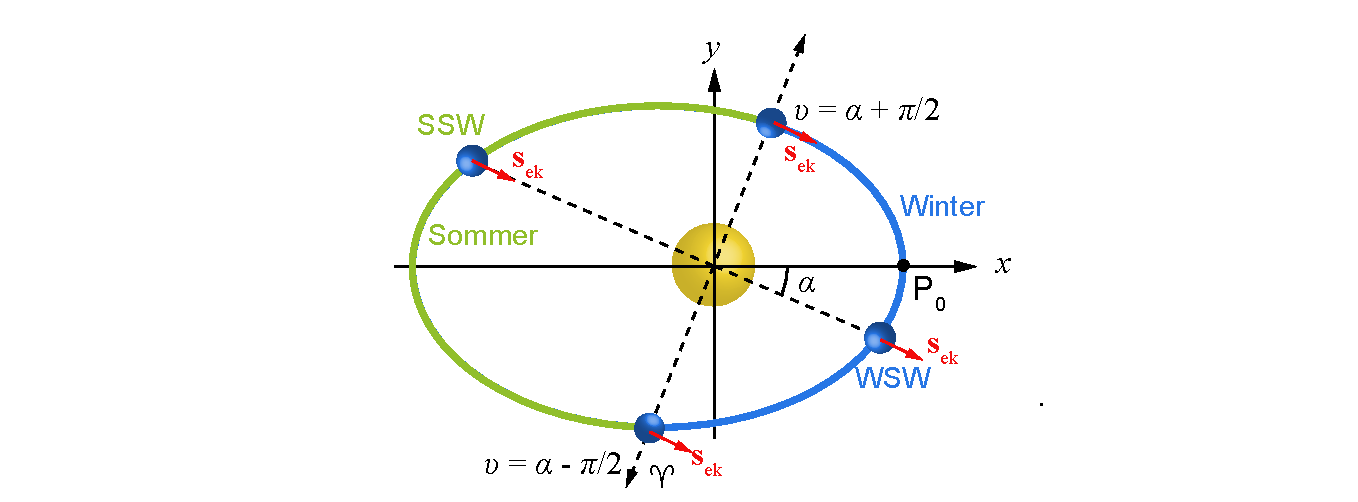
\includegraphics[width=\textwidth]{Erdbahn_im_Jahr_lsg2.pdf}%
	\caption{Erdbahn im Jahresverlauf}%
	\label{abb:hm_erdbahn_lsg_1}%
\end{figure}

	Wir definieren jetzt:
	\begin{align*}
		\text{Nordwinter: }& \alpha - \frac{\pi}{2} \leq \upsilon \leq \alpha+\frac{\pi}{2} ~~,\\
		\text{Nordsommer: }& \alpha + \frac{\pi}{2} \leq \upsilon \leq \alpha+\frac{3\pi}{2} ~~.
	\end{align*}
	Diese Halbjahre sind durch die Richtung der Erdachse gegeben und sind keineswegs gleich lang, wie wir gleich berechnen werden.
        Der gesamte Umlauf ben�tigt nach dem 3. Keplerschen Gesetz $T_\text{ges}\!=\!2\pi \sqrt{a^3/\mu_\text{G}}$.
        Die zeitliche Dauer des Sommerhalbjahrs ergibt sich dann mit Nutzung der Beziehungen
	\begin{align*}
		\frac{\D\upsilon}{\D t} &= \frac{L}{r^2} ~~\text{bzw.} ~~ \D t = \frac{r^2\,\D\upsilon}{L} ~,\;L = \sqrt{a\mu_\text{G}(1-e^2)} ~ \text{und}\;	r^2 = \lek \frac{a(1-e^2)}{1+e\cos\upsilon} \rek^2 ~~
	\end{align*}
	zu
	\begin{align}
   T_\text{Sommer} &= \frac{1}{L} \int\limits_{\alpha+\pi/2}^{\alpha+3\pi/2} r^2 \,\D\upsilon = \frac{a^2\lk 1-e^2\rk^2}{\sqrt{a\mu_\text{G}(1-e^2)}} \,\int\limits_{\alpha+\pi/2}^{\alpha+3\pi/2} \frac{1}{\lk 1+e\cos\upsilon\rk^2}\,\D\upsilon \nonumber\\
									 &= \frac{a^{3/2}\lk 1-e^2\rk^{3/2}}{\sqrt{\mu_\text{G}}} \,\underbrace{\int\limits_{0}^{\pi} \frac{1}{\lek 1-e\sin(\varphi+\alpha)\rek^2} \,\D\varphi}_{\equiv I} ~~, \label{eq:hm_erdbahn_lsg_5}
	\end{align}
	wobei wir $\cos(x+\pi/2)\!=\!-\sin x$ verwendet und $\varphi\!=\!\upsilon-(\alpha+\pi/2)$ gesetzt haben.
        Die L�sung des Integrals $I$ in \eqref{eq:hm_erdbahn_lsg_5} k�nnten wir wieder �ber \cite{Gradshteyn1980} erledigen.
        Wir wollen aber hier f�r kleine $e$ eine Reihenentwicklung durchf�hren:
	\begin{align*}
		I =&\, \int\limits_{0}^{\pi} \frac{1}{\lek 1-e\sin(\varphi+\alpha)\rek^2} \,\D\varphi \\
		  =&\, \int\limits_{0}^{\pi} \lek 1+2e\sin(\varphi+\alpha) + 3e^2\sin^2(\varphi+\alpha) + 4e^3\sin^3(\varphi+\alpha) \rek\,\D\varphi \\
		  =&\, \pi - 2e\cos(\varphi+\alpha) \bigg|_0^\pi + 3e^2 \lek -\frac{1}{4}\sin(2(\varphi+\alpha))+ \frac{1}{2}(\varphi+\alpha) \rek_0^\pi \\
			 &\, + 4e^3 \lek \frac{1}{12}\cos(3(\varphi+\alpha)) - \frac{3}{4}\cos(\varphi+\alpha)\rek_0^\pi \\
			=&\, \pi + 4e\cos\alpha+\frac{3}{2} e^2 \pi - 4e^3\,\frac{1}{6}\cos(3\alpha) + 6e^3\cos\alpha ~~.
	\end{align*}
	Damit erhalten wir
	\begin{align}
	T_\text{Sommer} =&\, \frac{a^{3/2}}{\sqrt{\mu_\text{G}}} \lk 1-\frac{3e^2}{2} + \mathcal{O}(e^4)\rk \lk \pi + 4e\cos\alpha + \frac{3e^2}{2} \pi - \frac{2e^3}{3}\cos (3\alpha) \right.\nonumber\\
	                 &\left. + 6e^3\cos\alpha +\mathcal{O}(e^4)\rk \nonumber\\
	              =&\, \frac{a^{3/2}}{\sqrt{\mu_\text{G}}} \lek \pi - \killA{\frac{3e^2}{2} \pi} + 4e\cos\alpha + \killA{\frac{3e^2}{2} \pi} - \killB{6e^3\cos\alpha} \right.\nonumber\\
                      &\left. -\frac{2e^3}{3}\cos(3\alpha) + \killB{6e^3\cos\alpha} + \mathcal{O}(e^4) \rek \nonumber\\
								=&\, \frac{a^{3/2}}{\sqrt{\mu_\text{G}}} \lek \pi + 4e\cos\alpha - \frac{2e^3}{3}\cos(3\alpha)\rek ~~.\label{eq:hm_erdbahn_lsg_6}
	\end{align}
	Wegen $T_\text{Winter}\!=\! T_\text{ges} - T_\text{Sommer}$ ergibt sich die Differenz der beiden Halbjahre zu
	\begin{align}
		\Delta T &= \frac{T_\text{Sommer} - T_\text{Winter}}{T_\text{ges}} = \frac{2T_\text{Sommer}}{T_\text{ges}}-1 \nonumber \\
		         &= \frac{2a^{3/2}\,\sqrt{\mu_\text{G}}}{\sqrt{\mu_\text{G}}\,2\pi\,a^{3/2}} \lek \pi+4e\cos\alpha-\frac{2e^3}{3}\cos^3(3\alpha)\rek -1 \nonumber \\
						&= \frac{4e}{\pi}\,\cos\alpha-\frac{2e^3}{3\pi}\,\cos(3\alpha) ~~. \label{eq:hm_erdbahn_lsg_7}
	\end{align}
	Die unterschiedliche Dauer der Jahreszeiten h�ngt also von der aktuellen Stellung der Erdachse (innerhalb ihrer Pr�zession) und der Elliptizit�t ab, nicht aber von der Neigung der Ekliptik.
        Der Winkel $\alpha$ ist der Winkel, den die Projektion der Erdachse auf die Ekliptik mit der Apsidenlinie bildet.
        Der Winkel $\alpha$ kann positiv oder negativ sein.
        Zum jetzigen Zeitpunkt (30.01.2021) ist dieser f�r die Erde negativ, da die Wintersonnenwende zeitlich vor dem Periheldurchgang liegt (\figref{hm_erdbahn_lsg_1}).
        Die Pr�zession der Erdachse �ndert sich aber $\alpha$ im Laufe der Zeit, was nach \eqref{eq:hm_erdbahn_lsg_6} bedeutet, dass sich auch die Dauer der Jahreszeiten �ndert. 
	\item Wir wollen jetzt den Eintrag der Sonne w�hrend eines Halbjahres berechnen und damit die Klimaeffekte absch�tzen.
          W�hrend eines Zeitraums $\D t$ erh�lt die Erde die Energie
	\begin{equation*}
	\D H = \frac{P_\text{\astrosun}}{4\pi r^2(\upsilon)}\,\pi R_\text{\earth}^2\,\D t = \frac{R_\text{\earth}^2}{4r^2(\upsilon)}\,P_\text{\astrosun}\,\frac{\D t}{\D\upsilon}\,\D\upsilon ~~,
	\end{equation*}
	wobei $P_\text{\astrosun}$ die Strahlungsleistung der Sonne und $R_\text{\earth}$ der Erdradius ist.
        Wir benutzen den bereits gut bekannten Trick mit dem Drehimpuls (\ldots was w�rden wir nur tun, wenn der keine Konstante w�re \ldots) und erhalten
	\begin{equation*}
	\D H = \frac{R_\text{\earth}^2 P_\text{\astrosun}}{4r^2(\upsilon)}\,\frac{r^2(\upsilon)}{L}\,\D\upsilon = \frac{1}{4}\,\frac{R_\text{\earth}^2 P_\text{\astrosun}}{\sqrt{a\mu_\text{G}(1-e^2)}}\,\D\upsilon ~~.
		\end{equation*}
	Die Energie in einem Jahr ist dann
	\begin{equation}
	H_\text{ges} = \int\limits_0^{2\pi} \D H = \frac{R_\text{\earth}^2 P_\text{\astrosun}}{4\sqrt{\mu_\text{G}}}\,\frac{2\pi}{\sqrt{a(1-e^2)}} = C_\text{H} \frac{2\pi}{\sqrt{a(1-e^2)}}~~,	\label{eq:hm_erdbahn_lsg_8}
	\end{equation}
	worin $C_\text{H}$ eine Konstante ist, die der Strahlungsleistung der Sonne direkt proportional ist.
        Wir k�nnen nat�rlich auch den Energieeintrag f�r ein Halbjahr berechnen:
	\begin{equation*}
	H_\text{Winter} = \int\limits_{\alpha-\pi/2}^{\alpha+\pi/2} \D H = \frac{H_\text{ges}}{2} ~~.
	\end{equation*}
	Danach w�ren die Energieeintr�ge f�r beide Halbjahre gleich gro�.
        Das ist etwas �berraschend, aber verst�ndlich, denn wir haben ja die komplette Querschnittsfl�che der Erde betrachtet, und �ber den Fl�chensatz werden die unterschiedlichen Halbjahresl�ngen zeitlich heraus gemittelt.
        Anders sieht es aus, wenn wir die Hemisph�ren (z.\,B.\, Nordhalbkugel) gesondert betrachten. 
	
	Wir betrachten dazu \figref{hm_erdbahn_lsg_2}. 
	\begin{figure}[H]
	\centering
	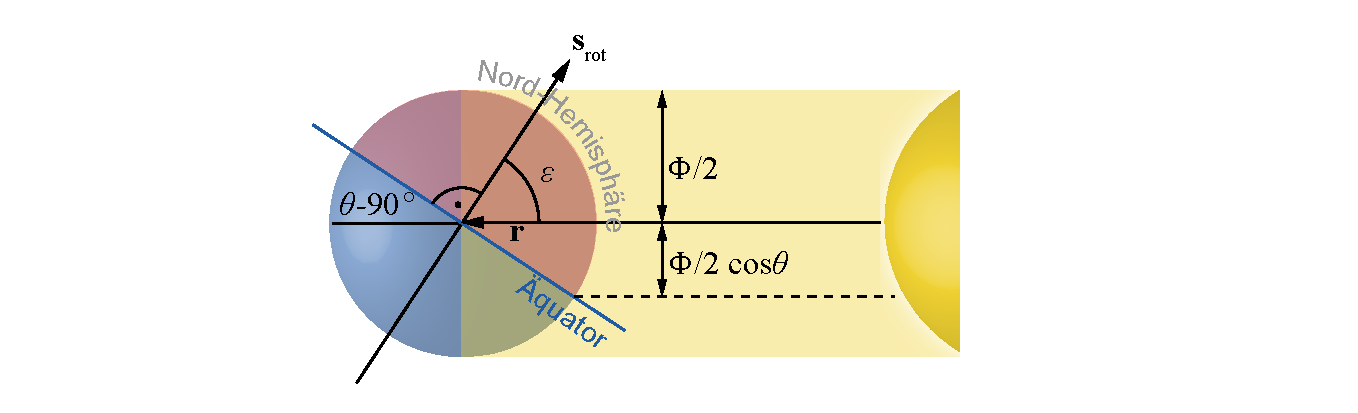
\includegraphics[width=\textwidth]{Erdbahn_im_Jahr_lsg3b.pdf}%
	\caption{Energieeintrag auf die Erde zur Sommersonnenwende}%
	\label{abb:hm_erdbahn_lsg_2}%
	\end{figure}
Der Sonnenlichtstrom $\Phi$ \anf{sieht} die Hemisph�ren unter einem Winkel $\theta$, der sich aus
	\begin{align*}
		\cos\theta(t) &= \frac{\vec{r}(\upsilon)\,\vec{s}_{\text{rot},\earth}}{\abs{\vec{r}(\upsilon)\,\vec{s}_{\text{rot},\earth}}} \nonumber\\
		              &= \lk \begin{matrix} \cos\upsilon(t) \\ \sin\upsilon(t) \\ 0 \end{matrix} \rk\,\lk \begin{matrix} \sin\epsilon \cos\alpha \\ \sin\epsilon\sin\alpha \\ \cos\epsilon \end{matrix} \rk  \\
									&= \sin\epsilon \lek \cos\alpha\cos\upsilon(t) + \sin\alpha\sin\upsilon(t)\rek \nonumber\\
									&= \sin\epsilon\,\cos\lek\upsilon(t)-\alpha\rek ~~ \nonumber
	\end{align*}
ergibt.
Die Sonneneinstrahlung trifft also je nach Jahreszeit auf unterschiedlich gro�e Teilfl�chen der jeweiligen Hemisph�re, der \anf{homogene} Strahlungsstrom verteilt $\Phi$ sich (wie im Bild zur Sommersonnenwende dargestellt) im Nordsommer auf die die Nord-Hemisph�re nach $(1\!+\!\cos\theta)/2$ und auf die S�d-Hemisph�re nach $(1\!-\!\cos\theta)/2$.
Wir berechnen jetzt den Energieeintrag pro "`Halbjahr"' und Hemisph�re und erhalten:
	\begin{align}
		H_\text{N,Sommer}&= C_\text{H}\,\frac{1}{\sqrt{a(1-e^2)}} \int\limits_{\alpha+\pi/2}^{\alpha+3\pi/2} \frac{\lek 1 + \sin\epsilon\cos(\upsilon-\alpha)\rek}{2}\, \D\upsilon \nonumber\\
		&= \frac{1}{2}\,C_\text{H}\,\frac{1}{\sqrt{a(1-e^2)}} \lek \pi-\sin\epsilon\sin(\upsilon-\alpha)\rek_{\alpha+\pi/2}^{\alpha+3\pi/2} \nonumber\\
		&= \frac{1}{2}\,C_\text{H}\,\frac{1}{\sqrt{a(1-e^2)}} (\pi+2\sin\epsilon) ~~.\label{eq:hm_erdbahn_lsg_10}
	\end{align}
	Eine analoge Beziehung erh�lt man f�r den Winter mit 
		\[H_\text{N,Winter} = \frac{C_\text{H}}{2}\,\frac{1}{\sqrt{a(1-e^2)}}\,(\pi-2\sin\epsilon) ~~,
	\]
woraus folgt:
\begin{equation}
\frac{\Delta H_\text{N}}{H_\text{ges}} = \frac{H_\text{N,Sommer} - H_\text{N,Winter}}{H_\text{ges}} = \frac{2\sin\epsilon}{\pi} ~~.\label{eq:hm_erdbahn_lsg_11}
\end{equation}
	
	Mit \eqref{eq:hm_erdbahn_lsg_10} und \eqref{eq:hm_erdbahn_lsg_6} k�nnen wir den durchschnittlichen Energieeintrag pro Zeit (also die empfangene Strahlungsleistung) in der n�rdlichen Hemisph�re f�r das Sommerhalbjahr berechnen:
	\begin{align}
		\frac{H_\text{N,Sommer}}{T_\text{Sommer}} &= P_\text{N,Sommer} \nonumber\\
		&= \frac{C_\text{H}\sqrt{\mu_\text{G}}(\pi+2\sin\epsilon)}{2\sqrt{a(1-e^2)}\, a^{3/2} \lek \pi+4e\cos\alpha-\frac{2e^3}{3}\cos(3\alpha)\rek} \nonumber\\
		&= \frac{P_\text{\astrosun}}{2}\,\lk\frac{R_\text{\earth}^2\sqrt{\mu_\text{G}}}{4\sqrt{\mu_\text{G}}\,a^2 \sqrt{1-e^2}}\rk \,\lk\frac{\pi+2\sin\epsilon}{\pi+4e\cos\alpha-\underbrace{\killA{\frac{2}{3}e^3\cos(3\alpha)}}_{\approx 0}}\rk \nonumber\\
		&\approx \frac{P_\text{\astrosun}}{8}\,\lk\frac{R_\text{\earth}^2}{a^2 \sqrt{1-e^2}}\rk \,\lk\frac{\pi+2\sin\epsilon}{\pi+4e\cos\alpha}\rk ~~.\label{eq:hm_erdbahn_lsg_12}
	\end{align}
	Wir k�nnen uns nun die tats�chlichen Werte und deren zeitliche Entwicklung anschauen.
        Wir finden dazu in den Tabellen \ref{tab:hm_bahnparameter} und \ref{tab:hm_zeitl_aenderung_bahnparameter_lin}
	\begin{align*}
		e &= 0.016709 - 3804\cdot 10^{-8}\,t ~~, \\
		\epsilon &= 23.4392911\degree + 46.8150''\,t =  23.4392911\degree + \frac{46.8150\degree}{3600} \,t ~~.
	\end{align*}
	Hier wird $t$ in Julianischen Jahrhunderten seit $J\,2000$ angegeben.
        F�r $\alpha$ k�nnen wir vereinfachend eine gleichm��ige Perihelpr�zession annehmen:
	\begin{equation*}
	\alpha(t) = \alpha_0 + 1.7192\degree \,t \approx -12.5\degree + 1.7192\degree \,t 
	\end{equation*}
	wobei wir die $1.7192\degree$ bereits als Ergebnis der Perihelverschiebung bzw. der unterschiedlichen L�ngen der tropischen und anomalistischen Jahre kennengelernt hatten.
	
	\begin{figure}[H]
	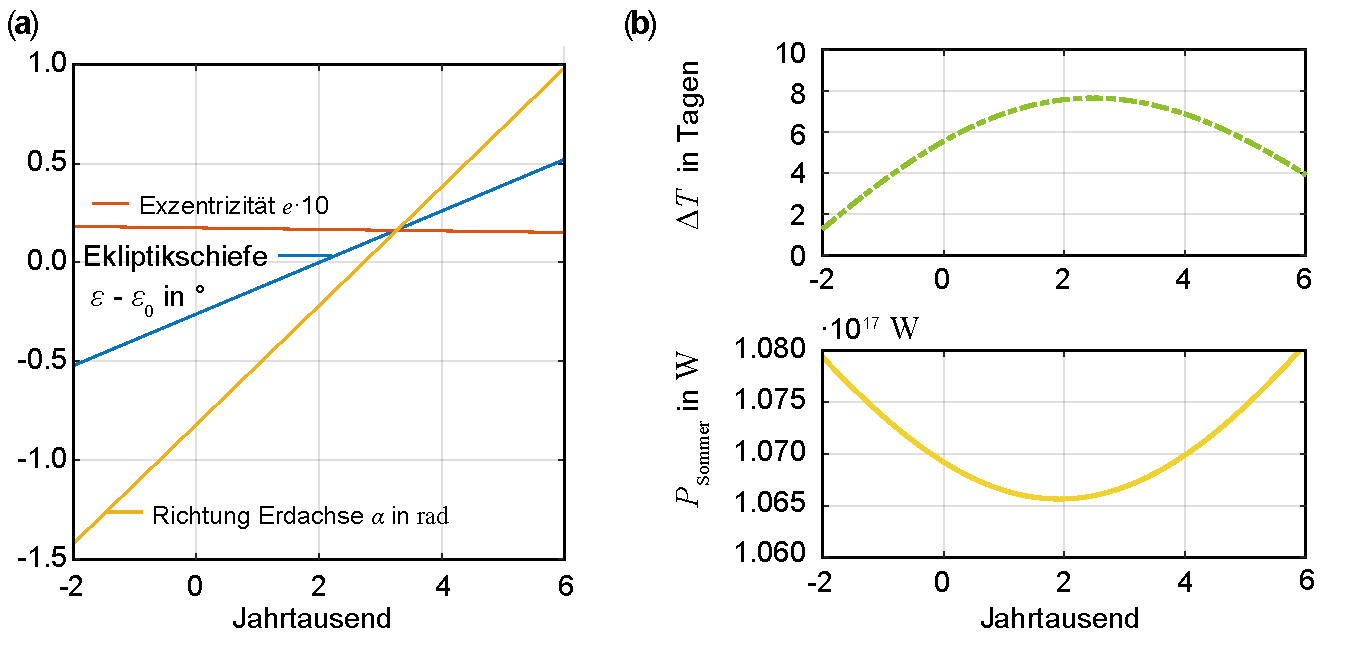
\includegraphics[width=\textwidth]{Erdbahn_im_Jahr_lsg_low.pdf}%
	\caption{Ver�nderung der zeitlichen Dauer der Jahreszeiten.}%
	\label{abb:hm_erdbahn_lsg_3}%
	\end{figure}
	
	In der \figref{hm_erdbahn_lsg_3} finden wir die Ver�nderung der zeitlichen Dauer der Jahreszeiten und auch den sich ver�ndernden  Energieeintrag f�r die Nord-Hemisph�re.
        Wir erkennen, dass wir uns im Moment in einer Trendwende befinden.
        Unser Sommerhalbjahr wird k�rzer werden.
        Gleichzeitig wird der mittlere Energieeintrag pro Halbjahr steigen.
        F�r langfristige Klimaeffekte kann man aber die Formel f�r $e$, $\epsilon$ und $\alpha$ nur bedingt benutzen, sondern muss Parametergleichungen als Funktion von $t$ finden, die einen Zeitraum von mehreren 100000 Jahren beschreiben \cite{Embacher2009}.
\end{enumerate}
\medskip
\end{sol} 
\textcolor{blue} {$\rightarrow$ zur} \probref{hm_erdbahn_im_jahr}.\\
\noindent\rule[1ex]{\textwidth}{0.5pt} \newpage

%-----------------------------------------------------------------------------------------------------------

\begin{sol}{prob:hm_refrak_optik}\label{lsg:hm_refrak_optik} %�bung11
\textbf{Refraktion -- ein Ausflug in die Optik} \\ \\
Wir beginnen mit dem planparallelen Modell (\figref{hm_refr_kugelschale_copy}).

\begin{figure}[H]
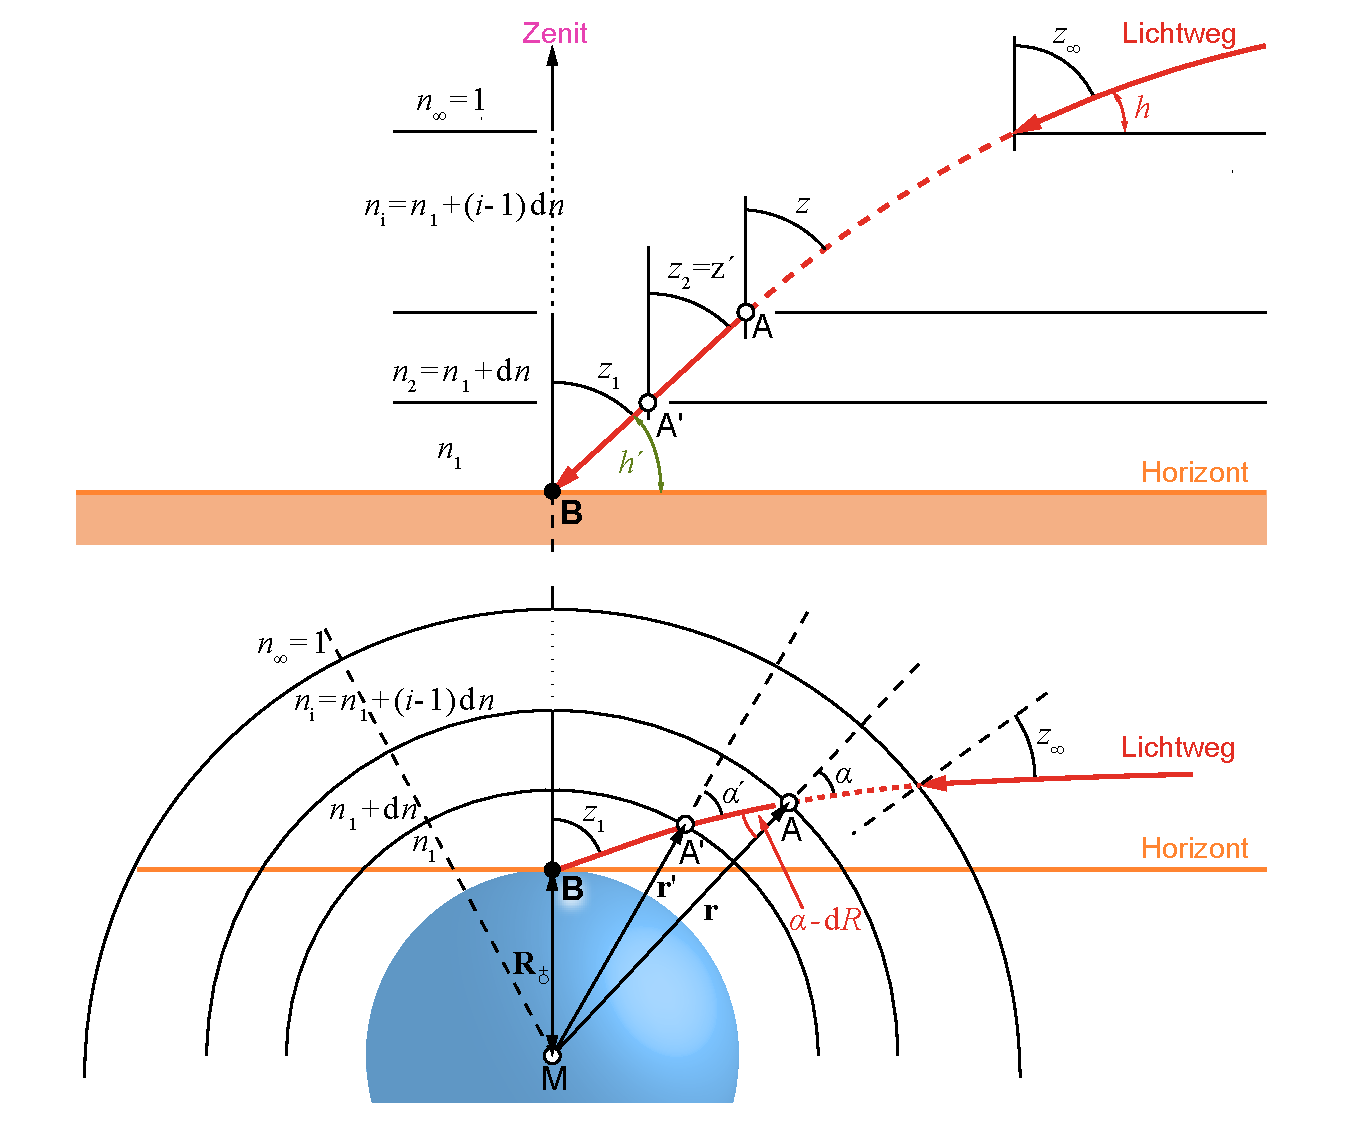
\includegraphics[width=\textwidth]{Refraktion0102.pdf}%
\caption[Planparalleles und Kugelschalen-Schichtenmodell.]{Planparalleles und Kugelschalen-Schichtenmodell zur Berechnung der Refraktion.
F�r die Winkel im $\bigtriangleup\mathrm{A}'\mathrm{MA}$ gilt: $\angle\mathrm{MA}'\mathrm{A}=180\degree-\alpha'$ und $\angle\mathrm{A}'\mathrm{MA}=\alpha-\D R$.}%
\label{abb:hm_refr_kugelschale_copy}%
\end{figure}
F�r die einzelnen Schichten mit unterschiedlichen Brechungsindizes $n_i$ k�nnen wir das Brechungsgesetz wie folgt aufschreiben:
\begin{equation}
n_1\,\sin z_1\,=\, n_2 \,\sin z_2\,=\,n_i\,\sin n_i\,=\,n_\infty\,\sin z_\infty ~~. \label{eq:hm_brechges_lsg12}
\end{equation}
Mit $z_\infty\!=\! [(90\degree - h]$,\, $z_1\!=\!90\degree - h'$,\, $n_\infty\!=\!1$ und der Definition $h\!=\!1h'-R$ folgt daraus
\begin{equation}
n_1\,\sin z_1 = \sin [(90\degree -h') + R] ~~. \label{eq:hm_R_lsg12a}
\end{equation}
Wie nehmen nun an, dass $R$ klein ist, was bei kleinen $z_\infty$ sicherlich gegeben ist und bekommen
\begin{align}
	n_1\,\sin z_1 &= \sin(90\degree - h') \, \cos R + \sin R \cos(90\degree - h')\, \nonumber \\
								& \approx \sin(90\degree - h') + R \cos(90\degree - h') = \sin z_1 + R \cos z_1 \nonumber \\
	\rightarrow ~~~~R &= (n_1 - 1)\,\tan z_1 ~~.  \label{eq:hm_R_lsg12b}
\end{align}
Die Refraktion\footnote{Ungl�cklicherweise bezeichnet man die Refraktion mit $R$, was oft zu Verwechslungen mit Radien und Abmessungen f�hrt. Da in der Literatur und insbesondere in Tabellen aber $R$ benutzt wird, halten wir uns ebenfalls an die Konvention.} $R$ ist also gegeben durch die im Allgemeinen unbekannte Brechzahl am Boden.
Man kann f�r Normalbedingungen und ein ideales Gas annehmen, dass die Brechzahl gem�� folgender Beziehung von der Dichte $\rho_\text{L}$ abh�ngt:
\begin{equation}
\frac{n^2-1}{n^2+2} \propto \rho_\text{L} = \frac{\bar{m}_\text{L} p_\text{L}}{R_0\,T} \label{eq:hm_brechzahl_von_dichte_lsg12}~~,
\end{equation}
worin $p_\text{L}$ der Luftdruck, $R_0\!=\! 8.31\!\cdot\! 10^3\:\text{J/(kmol\,K)}$ die Gaskonstante und $T$ die Temperatur ist.
Wir nehmen Normalbedingungen an, also $p_0\!=\! 101.325\:$kPa und $T_0\!=\! 293\:$K.
$\bar{m}_\text{L}\!\approx\! 28.95\:$kg/kmol ist das mittlere Molek�lgewicht des idealen Gases.
Aus \eqref{eq:hm_brechzahl_von_dichte_lsg12} kann man f�r $n\!\approx\!1$ schreiben:
\begin{equation}
\frac{(n+1)(n-1)}{n^2+2} \approx \frac{2}{3}\,(n-1) \propto \rho_\text{L} ~~.\label{eq:hm_glg4_lsg12}
\end{equation}
Setzt man \eqref{eq:hm_brechzahl_von_dichte_lsg12} und \eqref{eq:hm_glg4_lsg12} f�r verschiedene Temperaturen und Dr�cke ins Verh�ltnis, erh�lt man
\begin{align}
	n_1 - 1 &\approx (n_{10} - 1)\,\frac{p}{p_0}\,\frac{T_0}{T} = (n_{10} - 1)\, 2.6947\,\frac{p}{T} \nonumber\\
\Rightarrow R &= (n_{10}-1)\, 2.6947\,\frac{p}{T}\,\tan(90\degree - h') ~~.\label{eq:hm_glg5_lsg12}
\end{align}
Diese Beziehung f�r $R$ gilt nur f�r kleine $z_1$ oder gr��ere H�hen $h$, also nicht f�r den Fall der Berechnung des Sonnenaufgangs.
Wir wollen deshalb die Refraktion $R$ nach dem Kugelschalenmodell in \figref{hm_refr_kugelschale_copy}b berechnen und k�nnen hier das Brechungsgesetz f�r verschiedene Schichten wie folgt aufschreiben (Man betrachte Punkt A in \figref{hm_refr_kugelschale_copy}b.):
\begin{equation}
(n+ \D n)\,\sin(\alpha-\D R) = n\,\sin\alpha ~~. \label{eq:hm_glg6_lsg12}
\end{equation}
Wiederum ist $\D R$ eine kleine Gr��e, so dass aus \eqref{eq:hm_glg6_lsg12} gleich folgt:
\begin{align}
	(n+\D n)[\sin\alpha \underbrace{\cos(\D R)}_{\approx 1} - \cos\alpha \underbrace{\sin(\D R)}_{=\D R}] &= n\,\sin\alpha \nonumber\\
	\killA{n\,\sin\alpha} + \D n\,\sin\alpha - n\,\cos\alpha\,\D R &= \killA{n\,\sin\alpha} \nonumber\\
	\Rightarrow \D R &= \frac{\D n}{n}\,\tan\alpha ~~. \label{eq:hm_glg7_lsg12}
\end{align}
Wir ersetzen nun $\tan\alpha$ und benutzen dazu den Sinussatz im Dreieck $\bigtriangleup\text{MA'A}$:
\begin{equation}
\frac{\sin\alpha'}{r} = \frac{\sin(\alpha-\D R)}{r'} ~~. \label{eq:hm_glg8_lsg12}
\end{equation}
Kombinieren wir \eqref{eq:hm_glg6_lsg12} und \eqref{eq:hm_glg8_lsg12} erhalten wir durch Einsetzen von $\sin(\alpha-\D R)$
\begin{equation*}
r'(n + \D n)\,\sin\alpha' = rn\,\sin\alpha ~~.
\end{equation*}
Diese Beziehung gilt analog zu \eqref{eq:hm_brechges_lsg12} f�r alle Schichten.
Deshalb k�nnen wir schreiben:
\begin{equation}
rn(r)\,\sin\alpha = R_\text{\earth} n_1\,\sin z_1
\label{eq:hm_glg9_lsg12}~~.
\end{equation}
Wir benutzen jetzt noch die trigonometrische Beziehung $\tan\alpha = \sin\alpha/\sqrt{1-\sin^2\alpha}$ und k�nnen damit \eqref{eq:hm_glg7_lsg12} umformen zu
\begin{equation}
R(z_1) = \int \D R = \int\limits_{n=1}^{n=n_1} \frac{1}{n}\,\frac{A \sin z_1}{\sqrt{1-A^2\sin^2 z_1}} \,\D n \label{eq:hm_glg10_lsg12}
\end{equation}
mit 
	\[	A(n)\!=\frac{\!R_\text{\earth} n_1}{r n(r)} ~. 
	\]
Die Gleichung \eqref{eq:hm_glg10_lsg12} nennt man das Refraktionsintegral.\index{Refraktionsintegral}
Will man dieses auswerten, so muss man Annahmen f�r $n(r)$ bzw. $\rho_\text{L}(r)$ machen, die wiederum von $T(r)$ und $p(r)$ abh�ngen.
Im Allgemeinen wird das Integral numerisch gel�st.
Man kann dann auch beliebige Schichtmodelle annehmen und $ R$ �ber
\begin{equation*}
R = \sum_{i=1}^{i=N} \tan\alpha_i\,\lk\frac{n_{i+1} - n_i}{n_i}\rk
\end{equation*}
mit $\alpha_1\!=\! z_1\!=\! z_\text{schein}$ berechnen. 
Interessant ist noch, dass bereits Newton auf Basis seiner Korpuskulartheorie des Lichtes die Berechnung der Refraktion vornahm und diese als eine der kompliziertesten Aufgaben seines Lebens bezeichnete \cite{Nauenberg2017}. Er berechnete die Trajektorie des Lichtteilchens, welches durch die Brechung unter einer \emph{Zentralkraft} der Form
\begin{equation*}
\vec{F} = n\,\frac{\D n}{\D r} \frac{\vec{r}}{r}
\end{equation*}
steht.
Mit den Methoden, die wir in \kapitel{hm_bewegungsgl} dargestellt haben, insbesondere die Benutzung der Drehimpulserhaltung, kann man die Trajektorie des Teilchens als 
\begin{equation*}
z(r) = \bigintss\limits_{r_1 = R_\text{\earth}}^{r} \frac{\sin z_1}{r' \sqrt{\lk \frac{n(r') r'}{n_1 R_\text{\earth}} \rk^2 - \sin^2 z_1}} \D r'
\end{equation*}
und die Refraktion als
\begin{equation*}
R(z_1) = z_1 - z(r\rightarrow\infty) \equiv R(z') = z' - z 
\end{equation*}
schreiben \cite{Nauenberg2017}.
Wir wollen noch die Formulierung des Refraktionsintegrals f�r eine einfache Abh�ngigkeit der Brechungsindizes von der H�he angeben, der durch eine exponentielle Abnahme der Dichte nach
\begin{align*}
	\rho(r') = \rho(R_\text{\earth})\,\E^{-h/H} = \rho_0\,\E^{-h/H} ~~\text{mit} ~~ h = r - R_\text{\earth}
\end{align*}
nach folgender Formel 
\begin{align*}
	n(r') -1 = \kappa \,\frac{\rho(r')}{\rho(R_\text{\earth})} 
\end{align*}
gegeben ist, worin $\kappa$ und $H$ Konstanten der Erdatmosph�re sind.
In das Refraktionsintegral \eqref{eq:hm_glg10_lsg12} eingesetzt, ergibt das 
\begin{equation}
R(z_1) = \kappa \bigintss\limits_{0}^{\infty} \frac{\E^{-x}\,\sin z_1}{\lk 1+\kappa \E^{-x}\rk\,\sqrt{\lek \lk 1+\kappa \E^{-x} \rk \lk 1 + \frac{Hx}{R_\text{\earth}} \rk / \lk 1+\kappa\rk \rek^2 - \sin^2 z_1}} \:\D x ~~, \label{lsg:hm_refraktionsintegral2}
\end{equation}
welches wir in \mlhmref{Refraktion.m} f�r verschiedene Parameter $\kappa, H$ ausgewertet haben.
Als Parameter f�r einen relativ guten Fit an die Formel \eqref{eq:hm_Normalrefraktion1} haben wir aus der ISA-Tabelle \cite{ISA1976} die Werte $\kappa\!=\! 0.000316$ und $H\!=\! 9.87 $ km gew�hlt.

\begin{figure}[H]
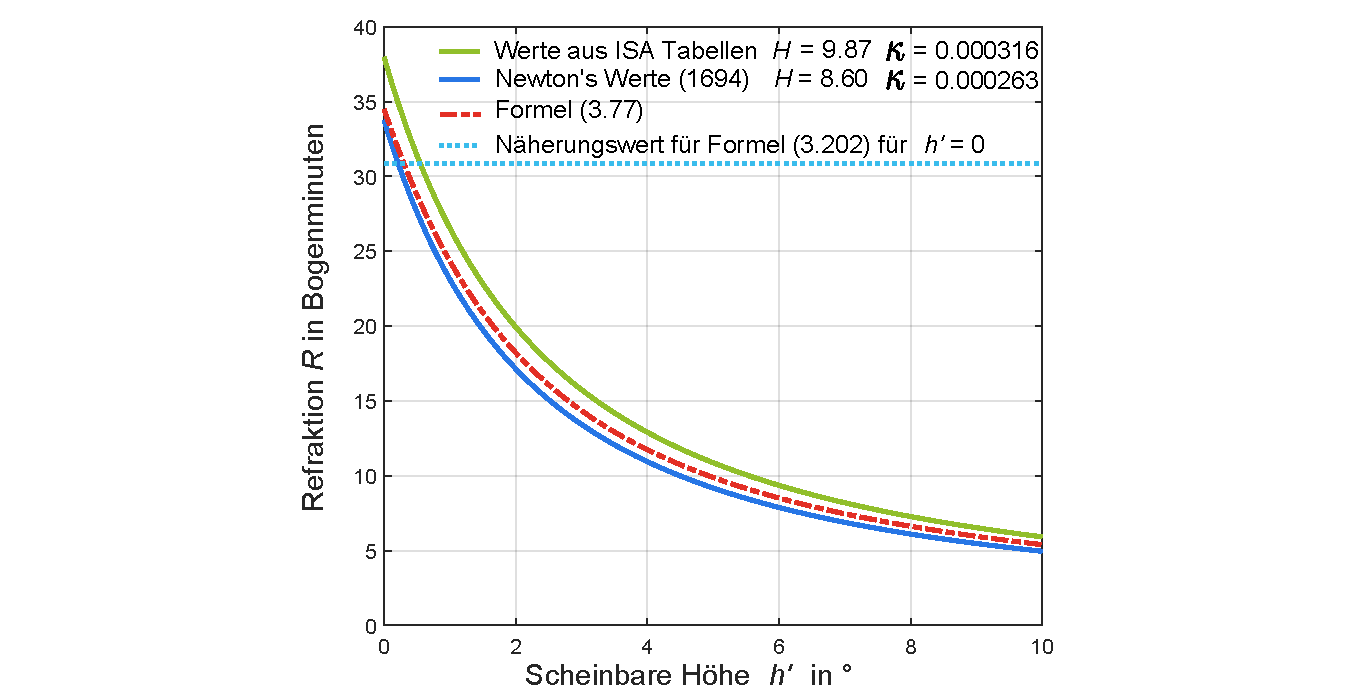
\includegraphics[width= \textwidth]{Refraktion12.pdf}%
\caption[Berechnete Refraktionskurven nach dem Kugelschalen-Schichtenmodell.]{Berechnete Refraktionskurven nach dem Kugelschalen-Schichtenmodell \eqref{lsg:hm_refraktionsintegral2} und Vergleich mit \eqref{eq:hm_relations2} sowie den Berechnungen von Newton \cite{Nauenberg2017}.}%
\label{abb:hm_Refraktion12}%
\end{figure}
\medskip \end{sol}
\textcolor{blue} {$\rightarrow$ zur} \probref{hm_refrak_optik}.\\
\noindent\rule[1ex]{\textwidth}{0.5pt} \newpage


\begin{sol}{prob:hm_abflachung_sonne} \label{lsg:hm_abflachung_sonne} %�bung12
\textbf{Abflachung der Sonne beim Untergang} \\

\begin{figure}[H]
\includegraphics[width=1.0\textwidth]{AbflachungSonne.pdf}%
\caption[Berechnung der Abflachung der Sonne bei Sonnenuntergang.]{Berechnete Form und H�he der Sonne mit (links) und ohne Refraktion (rechts). Bildmitte: Aufnahme Sonnenuntergang auf Hawaii (Bernd Geh am 10.11.2016 um 17:42:32) und dazu berechnete Form und Position.}%
\label{abb:hm_AbflachungSonne}%
\end{figure}

Wir benutzen zur L�sung die Refraktionsformel Formel \eqref{eq:hm_Normalrefraktion2}.
im Bild links sind die \anf{abgeflachten} Sonnen in der scheinbaren H�he zu sehen und rechts im Bild in gleicher Farbumrandung in astrometrische H�he und in der nicht durch Refraktion beeinflussten Form der \anf{Sonnenscheibe}.
In der Mitte ist ein auf Hawaii von Bernd Geh aufgenommenes Bild der untergehenden Sonne gefittet.
Wir verweisen auf \mlhmref{AbflachungSonne.m} und bedanken uns bei Bernd Geh (\href{http://www.bgeh-photography.com/Home.html}{http://www.bgeh-photography.com/Home.html}) f�r die Bereitstellung des Bildes und die Anregungen zur �bung.\\
\medskip \end{sol}
\textcolor{blue} {$\rightarrow$ zur} \probref{hm_abflachung_sonne}.\\
\noindent\rule[1ex]{\textwidth}{0.5pt} \newpage

\begin{sol}{prob:hm_tageslauf_sonne} \label{lsg:hm_tageslauf_sonne} %�bung13
\textbf{Tageslauf der Sonne} \\ \\
Wir verweisen auf das \mscr~\mlhmref{TageslaufSonne.m}. \\
\medskip \end{sol}
\textcolor{blue} {$\rightarrow$ zur} \probref{hm_tageslauf_sonne}.\\
\noindent\rule[1ex]{\textwidth}{0.5pt} \newpage

\begin{sol}{prob:hm_sonnenaufg_nyc}\label{lsg:hm_sonnenaufg_nyc} %�bung14
\textbf{Sonnenaufgang in New York City} \\ \\
Basierend auf \figref{hm_nyc_lsg} berechnen wir zun�chst aus der geographischen Breite $\varphi= 40.7\degree$ von New York City (NYC) den Radius des Erdellipsoids an dieser Stelle \cite{Meeus1998}:
\begin{align*}
	r_\text{NYC} &= \lek 0.9983271 + 0.0016764 \cos(2\varphi) - 0.0000035 \cos(4\varphi)\rek\, 6378137\:\text{m} \\
	&= 6369087\:\text{m}~.\\
\end{align*}

\begin{figure}[H]

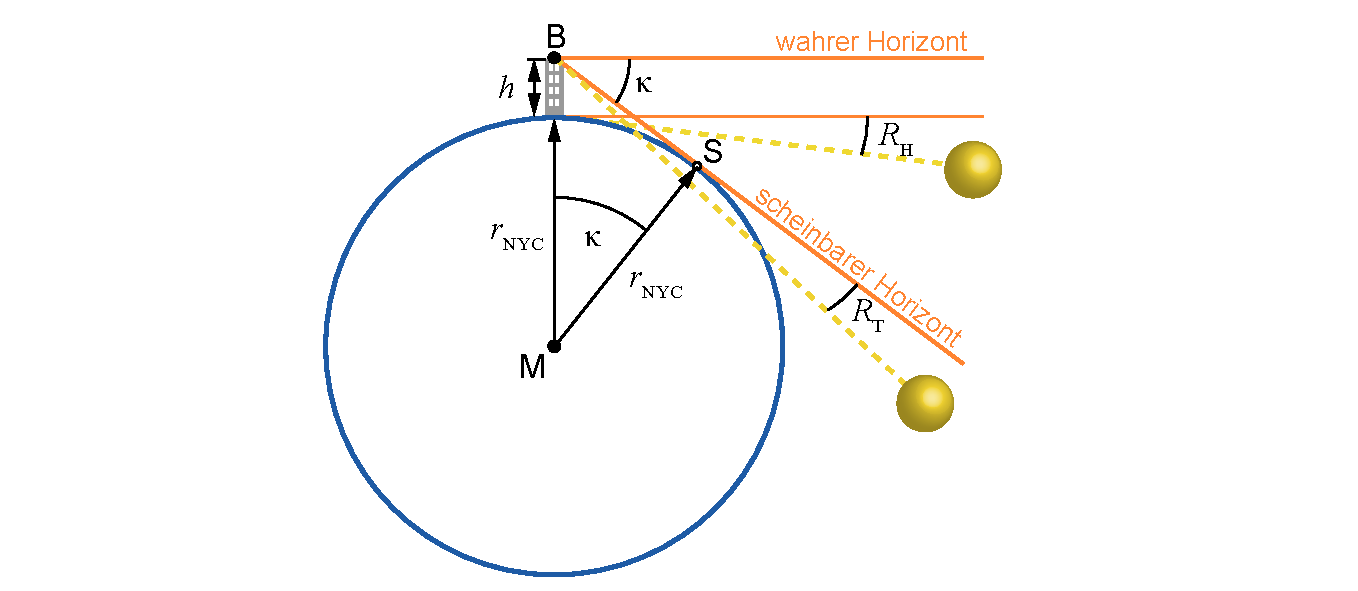
\includegraphics[width=\textwidth]{SonnenaufgangNYC.pdf}%
\caption{Geometrie zum Sonnenaufgang in New York City}%
\label{abb:hm_nyc_lsg}%
\end{figure}

Die H�he $h$ des One World Trade Centers betr�gt $531\:$m.
Daraus ergibt sich der Winkel $\kappa$ aus \figref{hm_nyc_lsg} �ber.
Es gilt weiterhin
\begin{align*}
	(r_\text{NYC} + h)^2 &= \overline{\text{BS}}^2 + r_\text{NYC}^2 \\
	\rightarrow \overline{\text{BS}} &\approx \sqrt{2\,h\,r_\text{NYC}} ~~\text{f�r}~~h\ll r_\text{NYC}~~.
\end{align*}
Es ergibt sich f�r kleine Winkel $\kappa$:
\begin{equation}
\tan \kappa \approx \sin \kappa = \frac{\overline{\text{BS}}}{r_\text{NYC}} = \sqrt{\frac{2h}{r_\text{NYC}}}~~,
\end{equation}
woraus $\kappa = 0.73981$ folgt.
Wir sehen ferner aus der Abbildung, dass ohne Ber�cksichtigung der Refraktion, der Sonnenaufgang um eine bestimmte Zeitdauer $\Delta t$ fr�her stattfindet.
$\Delta t$ entspricht der Zeit, die die Sonne br�uchte, um die H�he $h$ zu durchlaufen.
Wenn wir noch ber�cksichtigen, dass die Refraktion $R_\text{T}$ etwas gr��er ist als $R_\text{H}$,\footnote{Das Licht durchl�uft dichtere Luftschichten deutlich langsamer.} dann k�nnen wir f�r die Tagbogenverl�ngerung mit \eqref{eq:hm_tagbogverl} und $\delta\!= \epsilon\!\,$ folgendes aufschreiben:
\begin{align*}
	\Delta\tau_\text{B,H} &= -\frac{h_\text{r,H}}{\sqrt{\cos^2\delta - \sin^2\varphi}} = \frac{-16' - R_\text{H}}{\sqrt{\cos^2\delta - \sin^2\varphi}} ~~,\\
	\Delta \tau_\text{B,T} &= -\frac{h_\text{r,T}}{\sqrt{\cos^2\delta - \sin^2\varphi}} = \frac{-\kappa-16' - R_\text{T}}{\sqrt{\cos^2\delta - \sin^2\varphi}} ~~.
\end{align*}
Aus \eqref{eq:hm_Normalrefraktion1} finden wir zun�chst $R_\text{H} \!=\!R(0)\!\approx\! 34'$ und $R_\text{T} \!=\!R(-\kappa)\!\approx\! 45'$ und somit
\begin{align}
	\Delta t &= \Delta\tau_\text{B,1} - \Delta\tau_\text{B,0} \\
	        &= -\frac{(R_\text{T} - R_\text{H})+\kappa}{\sqrt{\cos^2 \delta - \sin^2 \varphi}} \\
					&\approx 5\:\text{min} ~ 45\:\text{s}~~.
\end{align}
Der Beobachter auf dem One World Trade Center sieht also die Sonne fast $6\:$min fr�her als jener auf Ellis Island.
Es lohnt sich also seinen Morgenkaffee auf dem One WTC zu trinken.\\
\medskip \end{sol}
\textcolor{blue} {$\rightarrow$ zur} \probref{hm_sonnenaufg_nyc}.\\
\noindent\rule[1ex]{\textwidth}{0.5pt} \newpage


%-----------------------------------------------------------------------------------------------------------

\begin{sol}{prob:hm_analytic_sunrise}\label{lsg:hm_analytic_sunrise} %�bung15
\textbf{Analytische Formel f�r den Sonnenaufgang und Sonnenuntergang} \\ \\
Wir folgen hier der Darstellung in \cite{Reinsch2003} und starten von der Beziehung f�r die astronomische H�he als Funktion des Stundenwinkels \eqref{eq:hm_Alt-Az-Koord}
\begin{equation*}
\sin h = \cos\delta \cos\tau \cos\varphi + \sin\delta \sin\varphi ~~.
\end{equation*}
Wir ersetzen die Deklination $\delta$ durch die geozentrisch-ekliptikale Koordinate $\lambda$ nach \eqref{eq:hm_drehung_x_achse_linear2} und erhalten mit $\beta\!=\!0$ und $\tau\!=\!\Theta-\alpha$ gem�� \eqref{eq:hm_std_winkel_tau} f�r die Sonne
\begin{align}
\sin h =&\, \underbrace{\cos\delta \cos\alpha}_{=\cos\lambda} \cos\Theta \cos\varphi + \underbrace{\cos\delta \sin\alpha}_{\sin\lambda \cos\epsilon} \sin\Theta \cos\varphi\, + \underbrace{\sin\delta}_{\sin\lambda \sin\epsilon} \sin\varphi \nonumber\\
			 =&\, \cos\lambda \cos\Theta \cos\varphi + \sin\lambda\cos\epsilon\sin\Theta\cos\varphi + \underbrace{\sin\lambda \sin\epsilon \sin\varphi}_{\equiv\text{T}_\text{II}} ~~. \label{eq:hm_sa_su_lsg1}
\end{align}
Die Aufgabe besteht nun darin, $\Theta(h\!=\!0)$ bzw. $\tau(h\!=\!0)$ f�r die Tage eines Jahres zu bestimmen.
Wir wollen dabei vereinfachend f�r die Sternzeit $\Theta$ annehmen, dass
\begin{equation}
\Theta = \frac{2\pi}{\text{d}_\diamond}\, t = \frac{2\pi}{86164\:\text{s}}\, t ~~. \label{eq:hm_sa_su_lsg2a}
\end{equation}
F�r die Weltzeit UT schreiben wir 
\begin{equation}
\hat{\Theta} = \frac{2\pi}{\text{d}_\text{\astrosun}}\, t = \frac{2\pi}{86400\:\text{s}}\, t ~~. \label{eq:hm_sa_su_lsg2b}
\end{equation}
Da wir besser die Uhrzeit und nicht die Sternzeit des Sonnenaufgangs bestimmen wollen, formen wir dies um zu
\begin{equation*}
\Delta (t) = \Theta - \hat{\Theta} ~~\text{bzw.}~~ \Theta = \hat{\Theta}+\Delta
\end{equation*}
und setzen diese Beziehung in \eqref{eq:hm_sa_su_lsg1} ein.
$\Delta (t)$ beschreibt im Prinzip das \anf{Auseinanderlaufen} von Sternzeit und Weltzeit, was exakt durch \eqref{eq:hm_UT_3} gegeben ist.
F�r unsere Absch�tzung des Sonnenaufgangs gen�gt aber der einfache Ansatz nach \eqref{eq:hm_sa_su_lsg2a} und \eqref{eq:hm_sa_su_lsg2b}.
Wir bekommen also
\begin{equation*}
\sin h = \underbrace{\cos\lambda \cos(\hat{\Theta}+\Delta) \cos\varphi + \sin\lambda \cos\epsilon \sin(\hat{\Theta}+\Delta) \cos\varphi}_{\equiv \text{T}_\text{I} = X \cos(\hat{\Theta}+\xi)\cos\varphi} + \text{T}_\text{II} ~~,
\end{equation*}
was eine algebraische Umformung unter Nutzung der Additionstheoreme ist. Mit den Termen
\begin{equation*}
X = \sqrt{\lk \cos\epsilon \sin\lambda \sin\Delta + \cos\lambda \cos\Delta \rk^2 + \lk \cos\epsilon \sin\lambda \cos\Delta - \cos\lambda \sin\Delta\rk^2}
\end{equation*}
und
\begin{equation*}
\xi = -\arctan \lk \frac{\cos\epsilon \sin\lambda \cos\Delta - \cos\lambda \sin\Delta}{\cos\epsilon \sin\lambda \sin\Delta + \cos\lambda \cos\Delta} \rk
\end{equation*}
erhalten wir schlie�lich
\begin{equation}
\sin h = \text{T}_\text{I} + \text{T}_\text{II} = X \cos (\hat{\Theta}+\xi) \cos\varphi + \sin\lambda \sin\epsilon \sin\varphi ~~.\label{eq:hm_sa_su_lsg3}
\end{equation}
Wir m�ssen jetzt eigentlich nur noch \eqref{eq:hm_sa_su_lsg3} nach $\hat{\Theta}$ f�r $h\!=\!0$ l�sen und machen hierzu die folgende N�herungen:
\begin{itemize}
	\item Vernachl�ssigung der Refraktion,
	\item Annahme, dass die ekliptikale L�nge $\lambda$ und $\Delta$ f�r die Dauer eines Tages konstant sind.
\end{itemize}
Wenn man mit \eqref{eq:hm_sa_su_lsg2a} mod $24\:$h bzw. mod $\pi$ nimmt und $h\!=\!0$ aus \eqref{eq:hm_sa_su_lsg3} benutzt, folgt daraus
\begin{equation}
\hat{\Theta}_\text{A,U} = \pm \arccos \lk - \frac{\sin\lambda \sin\epsilon \tan\varphi}{X} \rk - \xi ~~. \label{eq:hm_sa_su_lsg4}
\end{equation}
Dabei gilt das Minuszeichen f�r den Sonnenaufgang und das Pluszeichen f�r den Sonnenuntergang.
Laut unserer Definition der ekliptikalen L�nge ist ja am Fr�hlingspunkt $\lambda\!=\!0$ und die Uhren sind synchron  $\hat{\Theta} = \Theta$.
Es folgt demnach
\begin{equation*}
\hat{\Theta}_\text{A,U}(\vernal) = \underbrace{\tan \Delta(\vernal)}_{0} \pm \arccos (0) = \pm \frac{\pi}{2} = \pm 6\:\text{h} 
\end{equation*}
und damit der Sonnenaufgang als $\text{SA}\!=\!12\:\text{h}-\hat{\Theta}(\vernal) =$ 06:00h UT.
Wir haben mit \eqref{eq:hm_sa_su_lsg4} eine relativ �bersichtliche Formel f�r die Berechnung der Sonnenaufg�nge und Sonnenunterg�nge gefunden. 

\begin{figure}[H]
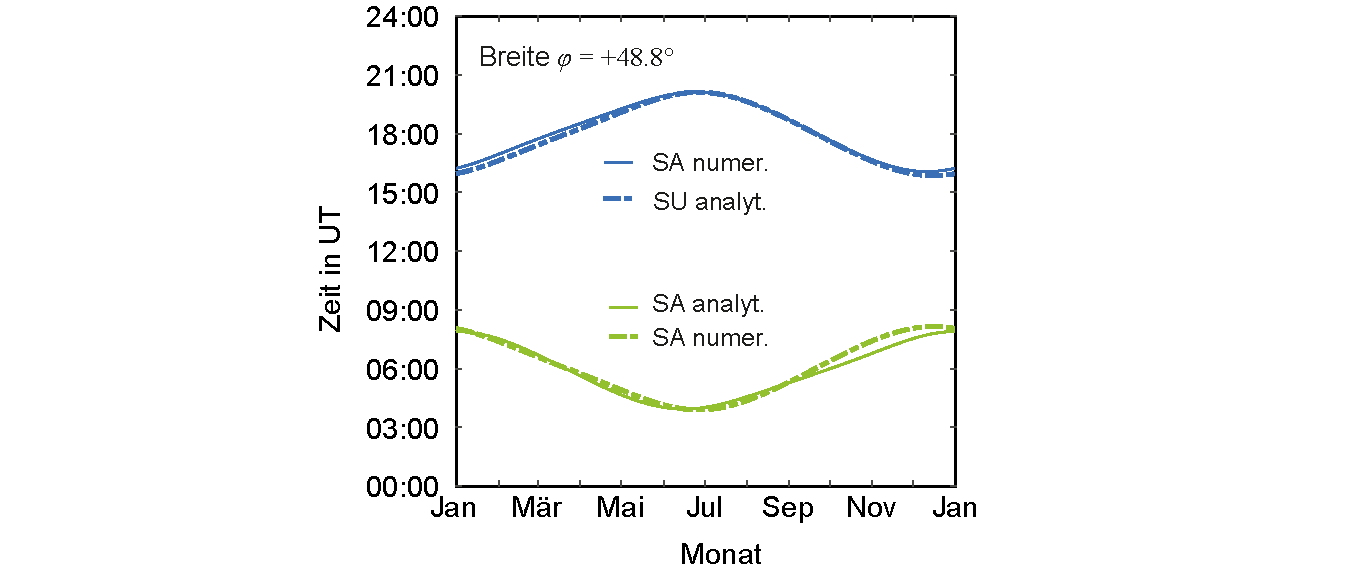
\includegraphics[width=\columnwidth]{Sunrise_lsg.pdf}%
\caption[Analytische und numerische L�sung Sonnenauf- und Sonnenuntergang.]{Analytische und numerische L�sung des Sonnenaufgangs und Sonnenuntergangs.}%
\label{abb:hm_sunrise_lsg}%
\end{figure}

Als Parameter f�r die N�herungsl�sung ben�tigen wir die L�nge des Sternen- und Sonnentags in Sekunden, die geographische Breite $\varphi$, die Ekliptikschiefe $\epsilon$ und die ekliptikale L�nge $\lambda$.
Letztere beschaffen wir uns wieder aus der Mittelpunktsgleichung \eqref{eq:hm_ekl_laenge_bogenmass}, womit in \eqref{eq:hm_sa_su_lsg4} wieder beide Effekte (Ekliptikschiefe und Elliptizit�t der Bahn) ber�cksichtigt worden sind.
In \figref{hm_sunrise_lsg} vergleichen wir die L�sung in \eqref{eq:hm_sa_su_lsg4} mit der numerischen L�sung, die �bereinstimmung ist relativ gut.
Es sei erw�hnt, dass die N�herungsformeln nicht gelten, wenn wir in den Bereich $\abs{\varphi}\!>\!+(90\degree\!-\!\epsilon)$ kommen.
Die analytische Formel wird dar�ber hinaus auch wegen des Verhaltens der $\arccos$-Funktion bei kleinen Argumenten f�r $\abs{\varphi}\!\ll\! \epsilon$ ungenau.
\medskip \end{sol}
\textcolor{blue} {$\rightarrow$ zur} \probref{hm_analytic_sunrise}.\\
\noindent\rule[1ex]{\textwidth}{0.5pt} \newpage


%-----------------------------------------------------------------------------------------------------------

\begin{sol}{prob:hm_VertikalAnalemmaSonnenuhr} \label{lsg:hm_VertikalAnalemmaSonnenuhr} %\�bung16
\textbf{Konstruktion von Sonnenuhren} \\

Konstruktion einer vertikalen und einer analemmatischen Sonnenuhr:
\begin{figure}%
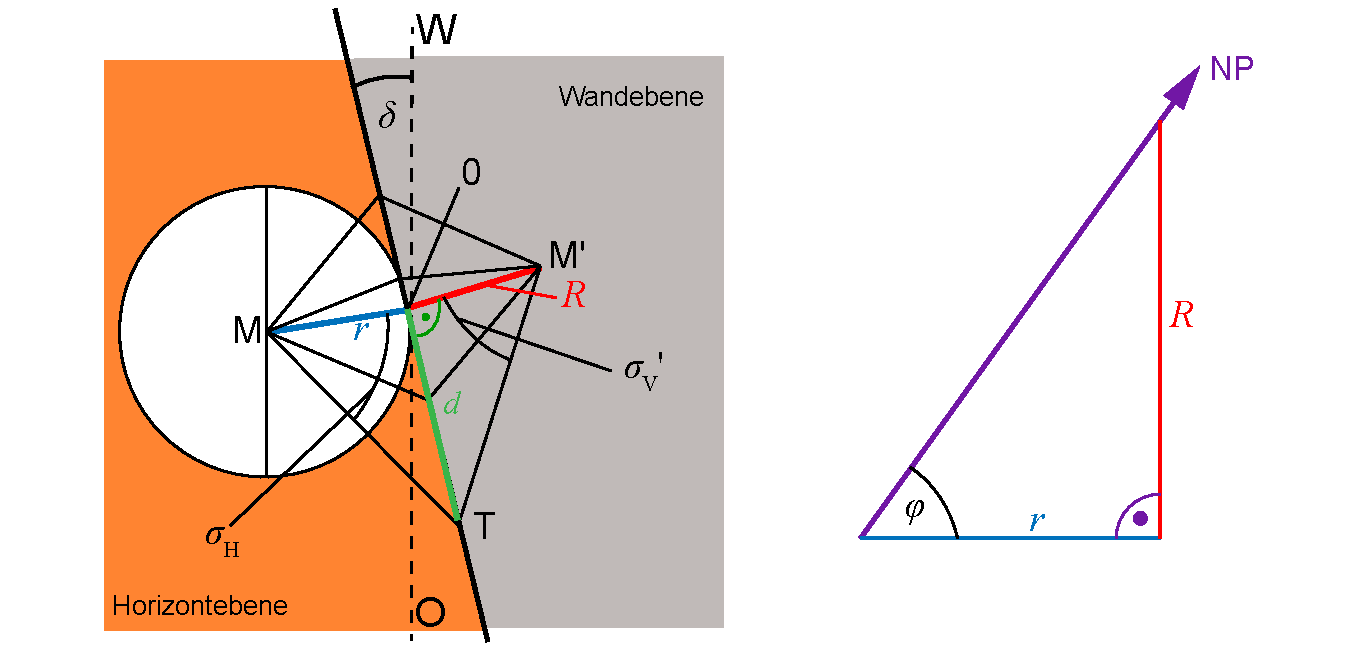
\includegraphics[width=\textwidth]{Sonnenuhr05.pdf}%
\caption[Ausf�hrung und Prinzip der Vertikal-Sonnenuhr.]{Ausf�hrung und Prinzip der Vertikal-Sonnenuhr bei  beliebiger Ausrichtung der Wand.}%
\label{abb:hm_sundial_lsg01}%
\end{figure}

\begin{enumerate}
 \item [a)]  

Wir betrachten zun�chst die Sonnenuhr, die an einer Hauswand angebracht ist, welche unter einem beliebigen Winkel $\delta$ zur Ost-West-Richtung steht.
Der Verdrehwinkel $\delta$ zur Wand sei negativ bei Ausrichtung SW-NO, wie im dargestellten Fall.
Aus \figref{hm_sundial_lsg01} lesen wir folgende Beziehungen ab:
    \begin{align}
        \tan\sigma_v{}' &= \frac{\overline{\text{0T}}}{R} = \frac{d}{R} \label{eq:hm_sundial_lsg01} \\
        \sphericalangle (\text{MT0}) &= 180\degree - (90\degree - \delta) - \sigma_\text{H} = 90\degree - (\sigma_\text{H} -\delta)\,. \label{eq:hm_sundial_lsg01a} 
    \end{align}
    Aus dem Sinussatz f�r das Dreieck $\Delta (\text{MT0})$ folgt:
    \begin{align}
        \frac{\sin\sigma_\text{H}}{d} = \frac{\sin \sphericalangle (\text{MT0})}{r} ~~~~\rightarrow ~~~~ d = r\,\frac{\sin\sigma_\text{H}}{\cos\lk \sigma_\text{H} - \delta \rk} \,. \label{eq:hm_sundial_lsg02}
    \end{align}
    Mit der Beziehung \eqref{eq:hm_sundial02} f�r die Radien $r$ und $R$ \,$ \tan\varphi = R/r$ und mit \eqref{eq:hm_sundial_lsg01} und \eqref{eq:hm_sundial_lsg02} folgt daraus:
    \begin{align}
        \tan\sigma_\text{V}{}' &= \frac{\sin\sigma_\text{H}}{\cos\lk \sigma_\text{H}- \delta\rk}\,\frac{1}{\tan\varphi} ~~~~ \text{mit} ~~~~ \sigma_\text{H} = \arctan \lk\sin\varphi\,\tan\sigma_\text{A} \rk \nonumber \\
				\rightarrow~\sigma_\text{V}{}' &= \arctan\lk \frac{\cos\varphi}{\cos\delta \cot\sigma_\text{A} + \sin\varphi \sin\delta}\rk	\,.
\label{eq:hm_sundial_lsg03}
    \end{align}
    F�r $\delta \to 0$ folgt daraus mit 
    \begin{align*}
        \tan\sigma_\text{V}{}' &= \frac{\sin\sigma_\text{H}}{\cos\sigma_\text{H}}\,\frac{1}{\tan \varphi} = \frac{\sin\varphi}{\tan\varphi}\,\tan\sigma_\text{A} = \cos\varphi\,\tan\sigma_\text{A} \\
    \end{align*}
    die Beziehung f�r die O-W ausgerichtete Wand.
    Die Lineatur f�r eine Sonnenuhr in Oberkochen ($\varphi = 48\degree$ N) und einer Wand die etwa ONO-WSW ausgerichtet ist ($\delta = -22.5\degree$) ist in \figref{hm_sundial_lsg02} zu sehen.\\

\begin{figure}%
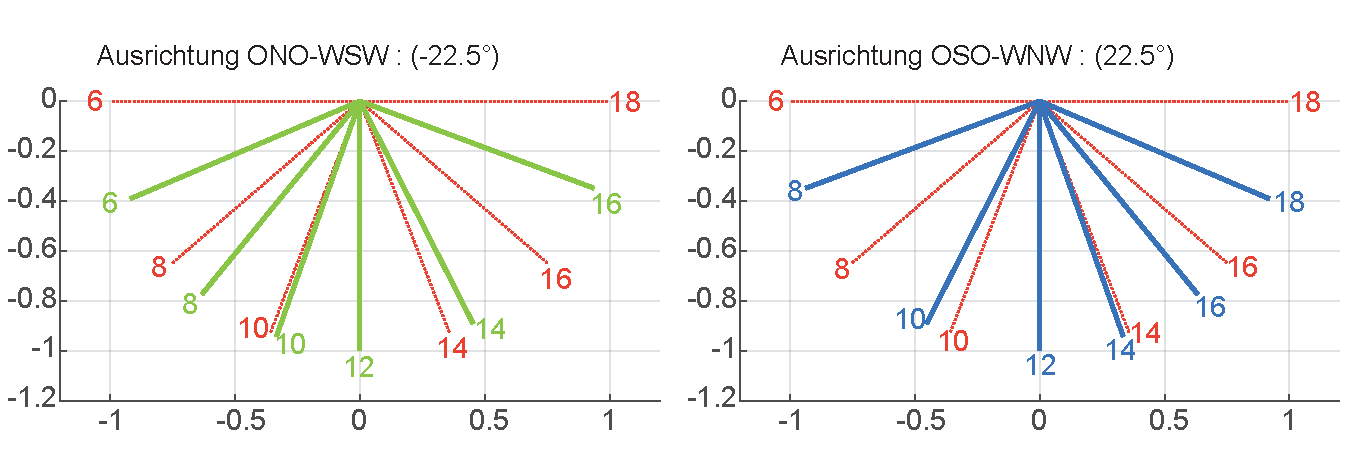
\includegraphics[width=\textwidth]{Wandsonnenuhr.pdf}%
\caption[Lineatur f�r eine Wandsonnenuhr in Oberkochen.]{Lineatur f�r eine Wandsonnenuhr in Oberkochen f�r verschiedene Ausrichtungen. Siehe \mlhmref{Wandsonnenuhr.m}} 
\label{abb:hm_sundial_lsg02}%
\end{figure}

\item [b)]

Nun wollen wir die Lineatur f�r eine analemmatischen Sonnenuhr in der Stadt G�rlitz (Breitengrad $\varphi = 51.2\degree$ und L�ngengrad $\lambda = 15\degree$) berechnen. 
Aus \eqref{eq:hm_sundial06} k�nnen wir die Abbildung $\vec{r}_n$ des Nodus aus der Sonnenrichtung $\vec{s}$ auf dem Ziffernblatt (welches in der Horizontalebene liegt) als Funktion des Datums und der Zeit, m.\,a.\,W.\ als Funktion des Sonnenstandes f�r eine bestimmte geographische Breite berechnen. \\
Wir k�nnen zur Berechnung nat�rlich vorteilhafter weise, die in \kap{hm_naeherungsformeln_sonne} berechneten Beziehungen f�r die H�he $h$ und das Azimut $\mathcal{A}$ der Sonne benutzen. Dann ergeben sich die Linien des Schatten des Nodus f�r einen bestimmten Tag eines Jahres $d_\text{fix}$ durch (wir nehmen die WSW, SSW und die Tag- und Nachtgleichen):
    \begin{align}
        \vec{r}_n (t) &= 
         \begin{pmatrix}
         \cos \lk h\lk t, d_\text{fix}\rk \rk \, \cos \lk \mathcal{A}\lk t,d_\text{fix} \rk\rk \\
         \cos \lk h\lk t, d_\text{fix}\rk \rk \, \sin \lk \mathcal{A}\lk t,d_\text{fix} \rk\rk \\
         0
         \end{pmatrix}\cdot
         \frac{H}{\sin h\lk t,d_\text{fix} \rk}\nonumber \\
          &= H\, 
         \begin{pmatrix}
             \cot\lk h\lk t,d_\text{fix}\rk\rk\,\cos\lk \mathcal{A}\lk t,d_\text{fix}\rk\rk\\
             \cot\lk h\lk t,d_\text{fix}\rk\rk\,\sin\lk \mathcal{A}\lk t,d_\text{fix}\rk\rk\\
             0
         \end{pmatrix} \,.  \label{eq:hm_lsgsundial11}
    \end{align}
    Analog ergibt sich f�r eine feste Uhrzeit $t_\text{fix}$ und die verschiedenen Tage $d$ des Jahres nat�rlich die Form des Analemma. 
    \begin{align}
        \vec{r}_n (d) = H\,
        \begin{pmatrix}
            \cot\lk h\lk t_\text{fix},d\rk \rk \, \cos\lk \mathcal{A}\lk t_\text{fix},d\rk \rk \\
            \cot\lk h\lk t_\text{fix},d\rk \rk \, \sin\lk \mathcal{A}\lk t_\text{fix},d\rk \rk \\
            0
        \end{pmatrix} \,.  \label{eq:hm_lsgsundial12}
    \end{align}
    $d$ steht hier f�r die Tage des Jahres. Die bei den Einzellineaturen nach \eqref{eq:hm_lsgsundial11} und \eqref{eq:hm_lsgsundial12} sind in \figref{hm_sundial_lsg03} zur Lineatur der Sonnenuhr zusammengesetzt.\\
    Eine besonders elegante analemmatische Sonnenuhr ist in Ref \cite{Heierli2019} beschrieben, die sich auch gut wie fast alle Sonnenuhren als Schmuckst�ck eignet. Wir verweisen auch auf die Aalener Sonnenuhr in der Zusatzaufgabe \probref{hm_Aalener_Sonnenuhr}, die in �hnlicher weise wie hier vorgestellt berechnet werden kann.
\end{enumerate}
\begin{figure}%
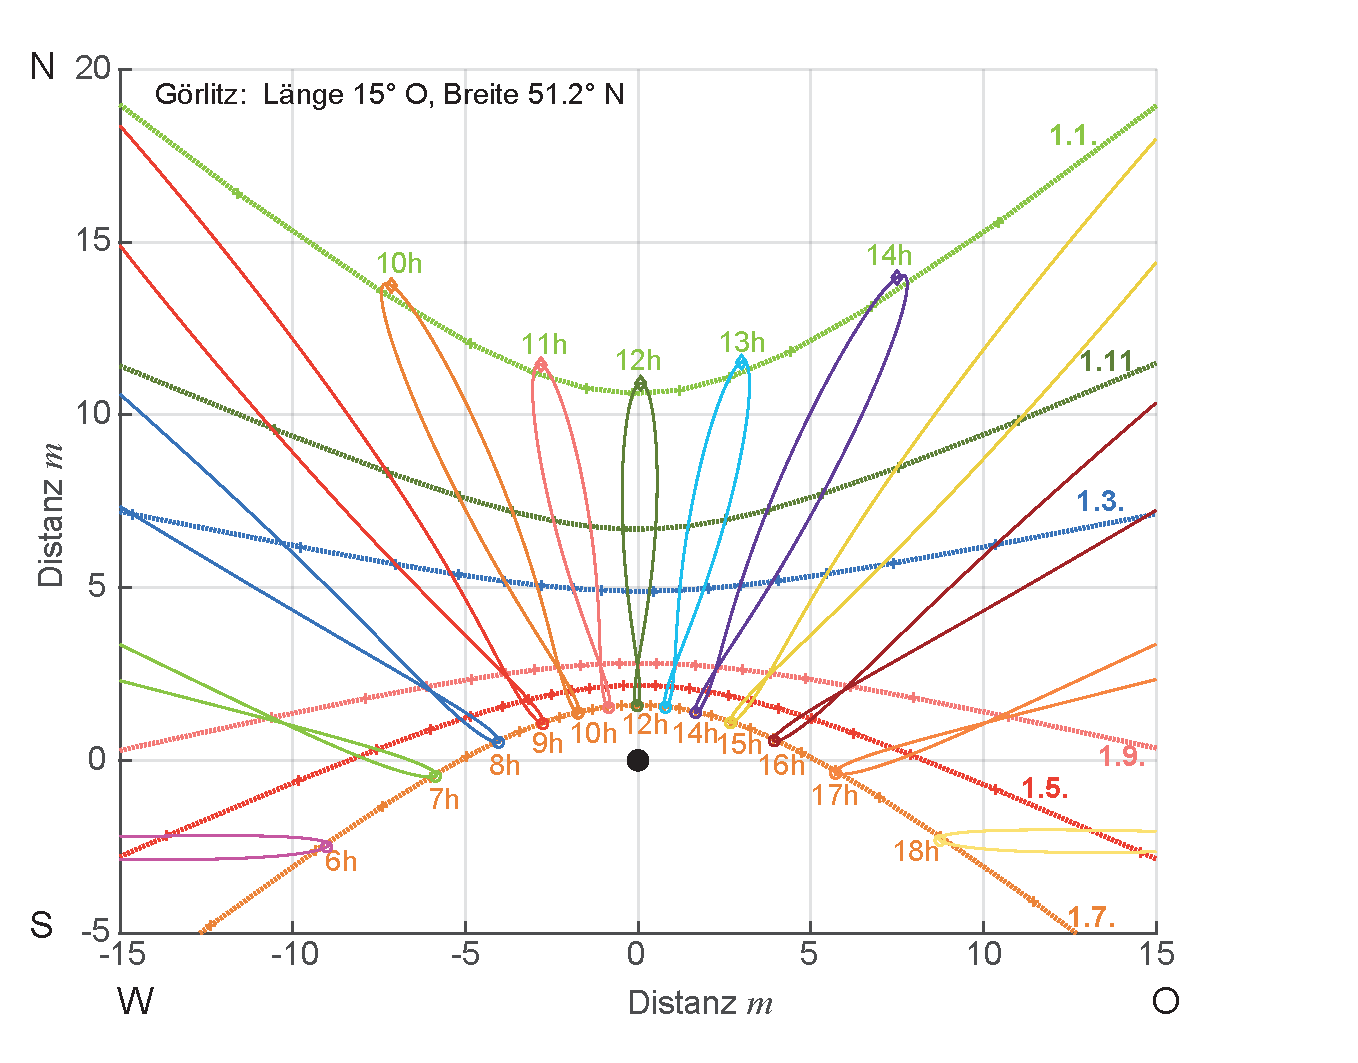
\includegraphics[width=\textwidth]{SonnenuhrAnalem.pdf}%
\caption[Berechnetes Ziffernblatt einer analemmatischen Sonnenuhr f�r G�rlitz.]{Berechnetes Ziffernblatt einer analemmatischen Sonnenuhr f�r G�rlitz. Siehe \mlhmref{SonnenuhrAnalem.m}} %
\label{abb:hm_sundial_lsg03}%
\end{figure}

\medskip \end{sol}
\textcolor{blue} {$\rightarrow$ zur} \probref{hm_VertikalAnalemmaSonnenuhr}.\\
\noindent\rule[1ex]{\textwidth}{0.5pt} \newpage


%-----------------------------------------------------------------------------------------------------------

\begin{sol}{prob:hm_opposition_mars}\label{lsg:hm_opposition_mars} %�bung17
\textbf{Mars-Oppositionen von 2000 bis 2020} \\ \\
Wir berechnen mit Hilfe der Gau�schen Vektoren die Bahnen von Mars und Erde in heliozentrischen Koordinaten und bestimmen die Zeitpunkte, an denen $l_\text{\mars}\!=\!l_\text{\earth}$ ist.
Es ergibt sich dann auch der minimale Abstand $\Delta r$.
Man sieht, dass auf Grund der relativ exzentrischen Bahn des Mars (\figref{hm_mars_opposition_lsg}), die Mars-Oppositionen nahe des Perihels dahingehend ausgezeichnet sind, dass der Mars der Erde besonders nahe kommt.
Wir m�ssen dann noch folgende Parameter berechnen:
\begin{itemize}
	\item Geozentrische Breite des Mars:
	   \begin{equation*}
		  \beta = \arcsin(z_\text{\mars}/\Delta r)
		 \end{equation*}
	\item Deklination des Mars zum Oppositionszeitpunkt \eqref{eq:hm_drehung_x_achse_linear2}:
		  \begin{equation*}
		  \delta = \arcsin(\cos\beta \sin l \sin\epsilon + \sin\beta \cos\epsilon) 
		 \end{equation*}
	\item H�he des Mars in Mitteleuropa zum Oppositionszeitpunkt\footnote{Man beachte, dass $\tau\!=\!0$ gesetzt (also dass Kulmination angenommen) wurde.} \eqref{eq:hm_Alt-Az-Koord}:
	    \begin{equation*}
		  h = \arcsin(\cos\delta\cos\varphi + \sin\delta \sin \varphi)
		 \end{equation*}
	\item Bildwinkel unter dem der Mars zum Oppositionszeitpunkt erscheint:
	     \begin{equation*}
		 \text{Bw} = \arcsin (R_\text{\mars}/ \Delta r)~~\text{mit}~~ R_\text{\mars} \approx 6770\:\text{km}
		 \end{equation*}
\end{itemize}
\begin{figure}[H]
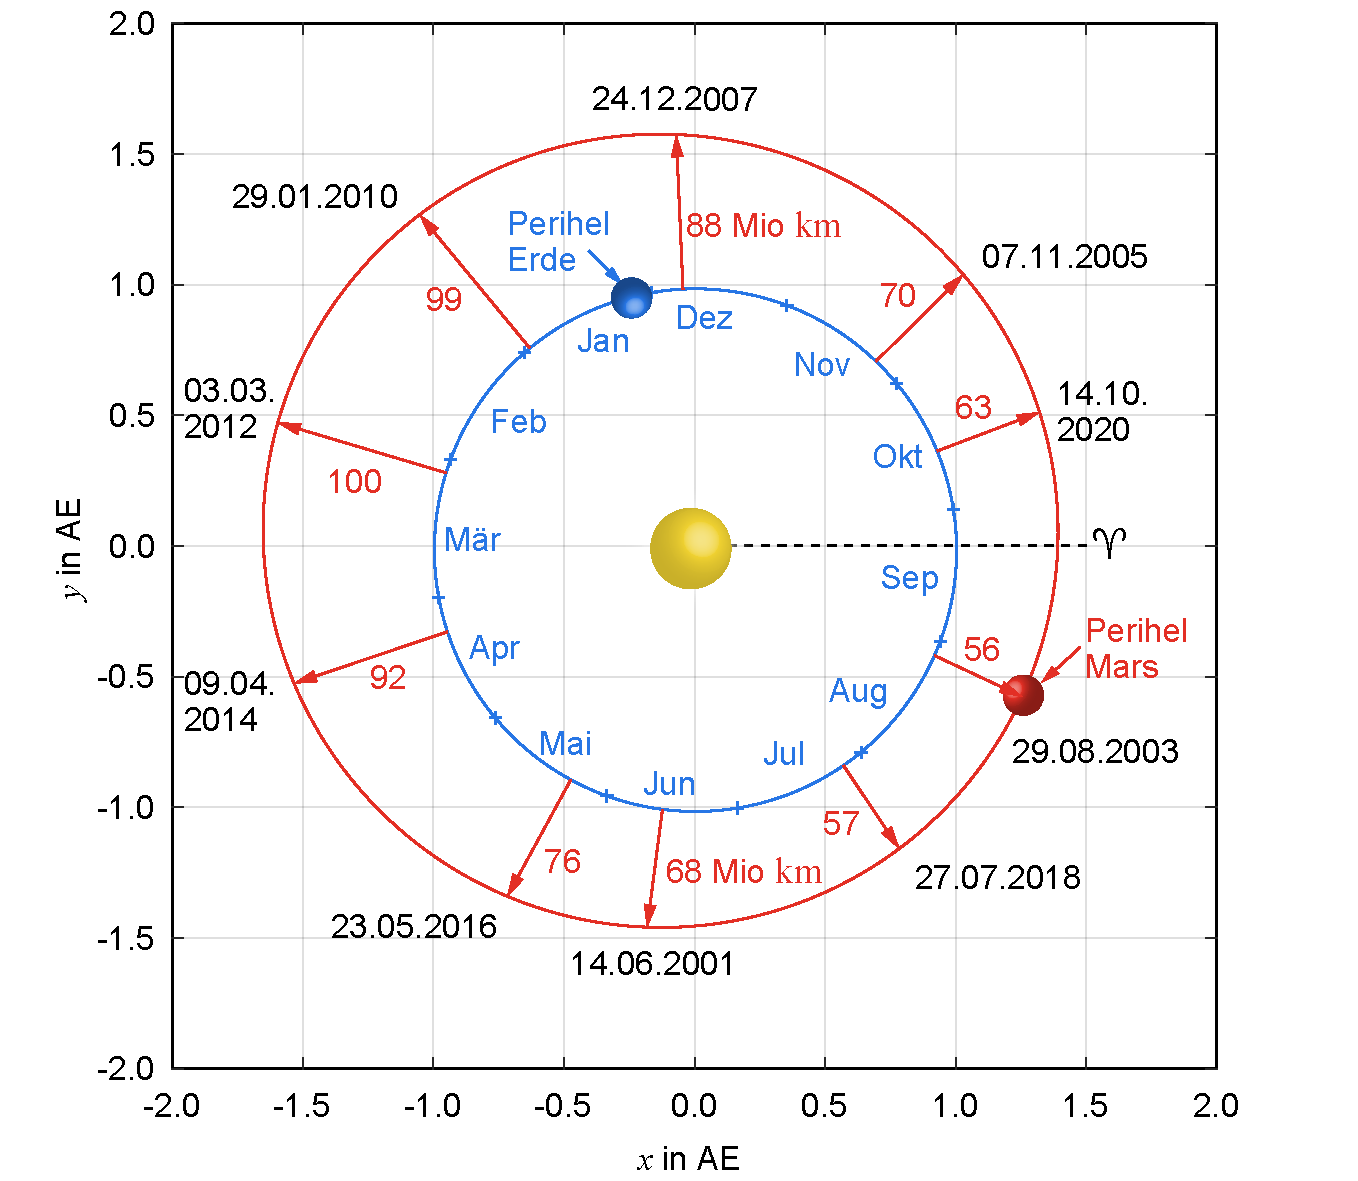
\includegraphics[width=\textwidth]{Mars_Opposition.pdf}%
\caption{Mars-Oppositionen im Zeitraum 2000 bis 2020}%
\label{abb:hm_mars_opposition_lsg}%
\end{figure}

\newpage
\begin{table}
\caption{Berechnung der Mars-Oppositionen von 2001 bis 2040}
\begin{tabular}{lR{1cm}R{1cm}R{1.5cm}R{1.5cm}R{1cm}R{1cm}R{1cm}R{1cm}}
\hline\noalign{\smallskip}
Datum	& $l\,[\degree]$ & $b\,[\degree]$ & $\Delta r\,[10^6\,\text{km}]$ & $R_\text{\mars}\,[10^6\,\text{km}]$ & $\beta\,[\degree]$ & $\delta\,[\degree]$ & $h\,[\degree]$ & $\text{Bw}\,['']$  \\
\noalign{\smallskip}\svhline\noalign{\smallskip}
14.06.2001 & 262.98 &	-1.02 &	67.80 &	219.10 &	-3.29 &	-26.54 &	14.66 &	20.60 \\
28.08.2003 & 335.09 &	-1.78 &	55.60	& 205.80 &	-6.62	& -15.79 &	25.41 &	25.13 \\
08.11.2005 & 45.70	& -0.13	& 70.40	& 218.00 &	-0.39	& 16.17	 &  57.37	& 19.85 \\
25.12.2007 & 93.05  &	1.27  & 88.60	& 235.00 &	3.38 &	26.78	 &  67.98	& 15.77 \\
30.01.2010 & 130.05	& 1.83	& 99.10	& 245.70 &  4.53	& 22.08	 &  63.28	& 14.10 \\
04.03.2012 & 163.78	& 1.69	& 100.40 & 248.00	& 4.17 &	10.23	 & 51.43	& 13.91 \\
10.04.2014 & 199.42 &	0.93	& 92.30	& 241.40	& 2.43	& -5.34	& 35.86	& 15.14 \\
23.05.2016 & 242.17	& -0.40	& 75.60	& 226.50	& -1.21	& -21.78 & 19.42 & 18.47 \\
27.07.2018 &	304.32 &	-1.79 &	57.40	& 208.50 & -6.49 & -25.48	& 15.72	& 24.32 \\
15.10.2020 &	21.49	& -0.87 &	62.70	& 211.20 & -2.94 &	5.65	& 46.85 & 22.28 \\
08.12.2022 &	76.10	& 0.83 &	82.10	& 228.80 &	2.31 &	25.01	& 66.21 &	17.02 \\
16.01.2025 &	116.10 &	1.70 &	96.00 &	242.40 &	4.29 &	25.14 &	66.34 &	14.55 \\
20.02.2027 &	150.93 &	1.81 &	101.00 & 248.10 &	4.46 &	15.31 &	56.51 &	13.83\\
25.03.2029 &	184.71 &	1.31 &	96.60	& 245.10 &	3.31 &	1.17 & 42.37 & 14.46 \\
04.05.2031 &	223.42 &	0.20 &	83.20	& 233.40 &	0.56 &	-15.33 & 25.87 &	16.79 \\
28.06.2033 &	276.69 &	-1.36 &	63.50	& 214.80 &	-4.59 &	-27.86 & 13.34 & 22.00 \\
17.09.2035 &	353.13 &	-1.54 &	57.00	& 206.60 &	-5.60	& -7.87 &	33.33	& 24.50 \\
20.11.2037 &	57.36  &	0.25 &	74.70	& 221.90 &	0.74 & 20.29 &	61.49	& 18.70 \\
03.01.2040 &	101.70 &	1.46 &	91.60	& 238.00 &	3.80 &	26.71 &	67.91 & 15.24 \\
\noalign{\smallskip}\hline\noalign{\smallskip}
\end{tabular}
\label{tab:hm_Mond-Mars-Abstand}
\end{table} 

In \figref{hm_mars_opposition_lsg} sind die Mars-Oppositionen f�r den Zeitraum 2000--2020 jeweils mit Datum und Abstand angegeben.
Man erkennt, dass bei Oppositionen in Periheln�he (z.\,B. am 29.08.2003) der Mars nahezu doppelt so gro� am Himmel erscheint\footnote{Tats�chlich konnte einer der Autoren (MK) am 29.08.2003 die Polkappen des Mars mit einem ZEISS APQ 135 ($5''$ Durchmesser und $2\:$m Brennweite) problemlos beobachten.
Gleich gute Chancen wird man in Europa erst wieder im Jahr 2035 haben.} wie bei Oppositionen in Apheln�he (z.\,B. am 03.03.2012).
Die Mars-Oppositionen f�r den Zeitraum 2001--2040 inklusive der f�r die Berechnung n�tigen Parameter sind in Tabelle \ref{tab:hm_Mond-Mars-Abstand} angegeben.\\

\medskip \end{sol}
\textcolor{blue} {$\rightarrow$ zur} \probref{hm_opposition_mars}.\\
\noindent\rule[1ex]{\textwidth}{0.5pt} \newpage


%-----------------------------------------------------------------------------------------------------------

\begin{sol}{prob:hm_venus_2004_2012}\label{lsg:hm_venus_2004_2012} %�bung18
\textbf{Venustransit-Beobachtungen 2004 und 2012} 

Vorbemerkung:\\
Beide Transits waren eine Jahrhundertereignis. Der n�chste Venustransit wird erst wieder 2117 zu beobachten sein. Wir bereiten mit dieser �bung aber schon mal die Berechnung vor. Ob man allerdings in 2117 noch eine \matlab{} Lizenz erwerben kann, ist nicht mit Sicherheit zu beantworten.

\begin{enumerate}[(a)] 
	\item Wir gehen von \figref{hm_VenusParallax} aus und betrachten den Fall, dass die Venus-Projektionen auf der Sonnenscheibe von den beiden Orten auf der Erde nicht symmetrisch zum Sonnenzentrum liegen.
          �ber die Geometrie der Winkel kann man zeigen, dass folgende Beziehungen gelten:
\begin{align*}
\nu_\text{\astrosun}+\nu_1 &= \nu_\text{\venus} + \nu_2 \\
\Rightarrow \Delta\nu &= \nu_1-\nu_2 ~~,
\end{align*}
woraus mit
\begin{align*}
\frac{\nu_\text{\venus}}{\nu_\text{\astrosun}} &= \frac{a_\text{\earth}}{a_\text{\venus}} \nonumber\\
\end{align*}
die Beziehung f�r die Astronomische Einheit 
\begin{equation}
a_\text{\earth} = \lk\frac{1}{\Delta\nu}\rk \lk\frac{d_\text{eff}}{\frac{a_\text{\earth}}{a_\text{\venus}} - 1}\rk = \frac{1}{\Delta\nu} \frac{d_\text{eff}}{\gamma - 1} \label{lsg:hm_venus_2004_2}
	\end{equation}
folgt.
\smallskip
Wir berechnen den effektiven Abstand $d_\text{eff}$ zwischen Troms� (N) und Canberra (AUS), in dem wir f�r die geographischen Koordinaten der Beobachtungsorte deren geozentrische Koordinaten verwenden.
Die Deklination f�r den Beobachtungsort entspricht dann der geographischen Breite (Abplattung der Erde vernachl�ssigt) und die Rektaszension ist einfach die Sternzeit berechnet nach \eqref{eq:hm_UT_3} zur Beobachtungszeit in UT.
Wir erhalten zu den Beobachtungsorten zwei Positions-Vektoren $\vec{r}_\text{T}$ und $\vec{r}_\text{C}$, deren Differenzvektor $\vec{r}_\text{d} = \vec{r}_\text{T}- \vec{r}_\text{C}$ unter einem Winkel $w$ zum Richtungsvektor Erdmittelpunkt -- Sonne ($\cos\delta\cos\alpha$, $\cos\delta\sin\alpha$, $\sin\delta$) steht.
Wir berechnen den Kosinus dieses Winkel $w$ aus dem Skalarprodukt.
Die effektive L�nge ist dann gegeben durch 
\begin{equation*}
d_\text{eff}=\left| \vec{r}_\text{d} \right|\sin w ~~.
\end{equation*}
F�r die Werte am 06.\,06.\,2012 sind die einzelnen Berechnungen in \mlhmref{VenusMerkurTransit.m} ausgef�hrt und numerisch ergibt sich $d_\text{eff}\!=\!11415 \:\text{km}$. \\
Ein sehr sch�ne Auswertung f�r die Berechnung der AE bei Beobachtung der Transitdauer an zwei Standorten findet sich in \cite{Messmer2004}. \\
\smallskip

	\item Wir gehen nun �ber zu der Auswertung der Transitdaten von nur einem Standort.
          Dazu muss man wie im  Beispiel \ref{bsp:venustransit} ausgef�hrt auf die t�gliche Parallaxe zur�ck greifen.
          Aus der Abbildung des Beispiels \ref{bsp:venustransit} k�nnen wir die folgende Beziehung ableiten:
	\begin{align}
	\frac{\D s_\text{\venus}-\D s_\text{\earth}}{a_\text{\earth}-a_\text{\venus}}&=\frac{\D P_\text{B} - \D s_\text{\earth}}{a_\text{\earth}}~,\nonumber\\
	\Rightarrow \frac{a_\text{\venus}}{a_\text{\earth}-a_\text{\venus}} \lk \frac{\D s_\text{\venus}}{a_\text{\venus}} - \frac{\D s_\text{\earth}}{a_\text{\earth}} \rk &= \frac{\D P_\text{B}}{a_\text{\earth}} ~,\nonumber \\
	\stackrel{\, 1/\D t}{\Rightarrow} \lk\frac{1}{\gamma -1}\rk \lk  \omega_\text{\venus} - \omega_\text{\earth} \rk &= \Omega_\text{B} ~~. \label{lsg:hm_venus_2004_3}
	\end{align}
Dabei haben wir $\gamma\!=\!a_\text{\earth} / a_\text{\venus}$, $\D s_i\!=\!\omega_i a_i \D t$ und $\D P_\text{B}\!=\!\Omega_\text{B} a_\text{\earth} \D t$ benutzt.
\smallskip
Wir berechnen den effektiven Abstand $d_\text{eff}$ f�r die Beobachtungen am 08.06.2004 in Oberkochen ($\phi\!=\!48.8\degree$ N, $\lambda\!=\!10.1\degree$ O) wieder wie oben, indem wir f�r die geographischen Koordinaten der Beobachtungszeitpunkte die geozentrische Koordinaten verwenden.
Die Deklination entspricht dann der geographischen Breite und die Rektaszensionen der Sternzeiten berechnet nach \eqref{eq:hm_UT_3} zum Anfangs- und Endzeitpunkt des Transits.
F�r gemessene Zeiten f�r Transitbeginn 07:16 MESZ $\pm 1$ min und Transitende 13:18 MESZ $\pm 1$ min ergibt sich eine effektive Entfernung von $d_\text{eff}\!=\!4444\:\text{km}$.
Die relative Sehnenl�nge konnte dabei zu 0.775 bestimmt werden (Messdaten MK).
Mit der Berechnungsformel aus dem Beispiel
\begin{equation}
a_\text{\earth}=\lk\frac{d_\text{eff}}{\gamma-1}\rk \lk\frac{1}{{l_\text{S\astrosun}}{b_\text{w\astrosun}}-\Omega_\text{B} T_\text{TR,B }}\rk \label{lsg:hm_venus_2004_4}
\end{equation}
erhalten wir daraus als Mittelwert f�r $\text{AE}\!=\!115\cdot 10^6\:$km.
Tr�gt man den relativen Fehler als Funktion der gemessenen Transitzeit auf, so sieht man, dass schon bei Unsicherheiten in der gemessenen Transitzeit von $60\:\text{s}$ ein Fehler von $20\%$ in der Bestimmung der astronomischen Einheit resultiert (\figref{hm_Kontaktzeit_lsg}a.
Das liegt daran, dass die Abh�ngigkeit von der gemessenen Transitzeit, bei dem gegen Null gehenden Nenner in \eqref{lsg:hm_venus_2004_3} sehr gro� ist (\figref{hm_Kontaktzeit_lsg}b.
Genau so kritisch ist die Messung der Sehnenl�nge $l_\text {S}$ des Transits.
Im Rahmen der Messgenauigkeit ergab sich ein Mittelwert von $115\cdot 10^6\:\text{km} $.\footnote{Der Mittelwert ist tendenziell ein eher zu kleiner Wert, was vermuten l�sst, dass die Messzeit als zu kurz eingesch�tzt wurde.
Es ist au�erordentlich schwierig, am Rand der Sonne genau Beginn und Ende des Transits festzustellen.}
\begin{figure}[H]
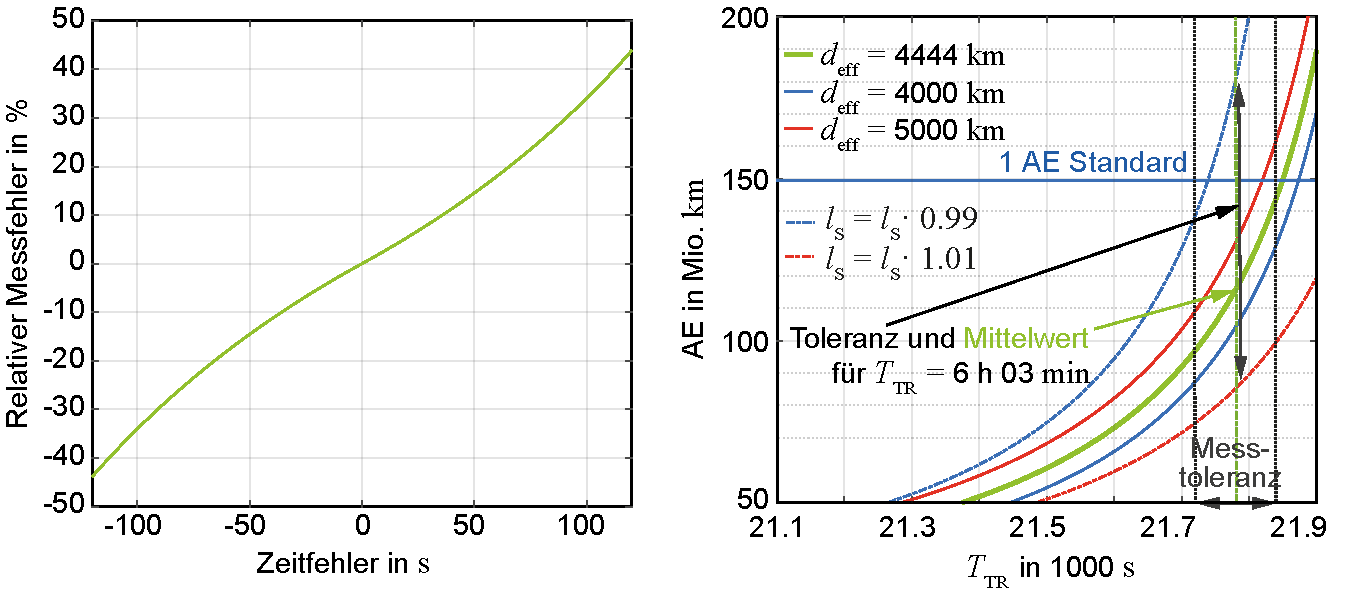
\includegraphics[width=\columnwidth]{KontaktzeitmethodeAE.pdf}%
\caption{Fehler in der Bestimmung der AE bei der Kontaktzeitmethode}%
\label{abb:hm_Kontaktzeit_lsg}%
\end{figure}
Ein verbesserte Auswertung f�r die Berechnung der AE bei Beobachtung der Transitdauer an nur einem Standorten findet sich \cite{Brodbeck2004}. \\

	\item Wir ber�cksichtigen jetzt f�r den Fall, dass die Beobachtung nur an einem Ort der Erde stattfinden kann.
          sowohl die Elliptizit�t der Bahnen, als auch die Neigung der Venusbahn gegen die Ekliptik und die topozentrischen Koordinaten des Beobachters.
          Diese Berechnung geht auf den Astronomen James Short\footnote{James Short (1710--1768) war ein britischer Mathematiker, Optiker und begnadeter Teleskopbauer.
          Wir empfehlen dazu auch den lesenswerten Artikel \cite{Teets2003}, auf dessen Basis die L�sung der �bung strukturiert wurde.} zur�ck, der viele der Messungen von 1761 systematisch auswertete und dessen ermittelte Sonnenparallaxe von $8.65''$ �quivalent zu $a_\text{\earth}\!=\!154.4\cdot 10^6 \:\text{km}$ lange als Referenz f�r die AE galt.
          Die Rechnungen sind im Detail in \mlhmref{VenusMerkurTransit.m} ausgef�hrt.
          Eine Betrachtung f�r n�herungsweise konzentrisch und koplanar angenommene Planetenbahnen kann man in \cite{Messmer2004} bzw. \cite{Brodbeck2004} finden. \\
Um den Transit in seiner allgemeinen Form zu berechnen, m�ssen wir zwei KOS zueinander in Beziehung setzen:
\begin{enumerate}[A.]
	\item Das GA(sf) KOS (\figref{hm_venustransit_lsg_2a}), was f�r den Beobachter des Transits das ausgezeichnete KOS ist und folgenderma�en definiert ist:
	Die $x'$-Achse zeigt zum Fr�hlingspunkt und beh�lt ihre Richtung im Raum bei, die $z'$-Achse ist die Rotationsachse der Erde.
	\begin{enumerate}[1.]
	\item Die t�gliche Rotation der Erde beschreiben wir mit 
\begin{equation}
\theta = \theta_0 + \frac{15\degree}{\text{h}}\, (t-t_0)~~,
\label{eq:hm_venustr_d_3}
\end{equation}
worin $\theta_0\!=\!\GMST$ und die Zeiten $t$, $t_0$ in UT angegeben werden.
$t_0$ soll dabei die Zeit der Transitmitte sein.
\begin{figure}[H]
	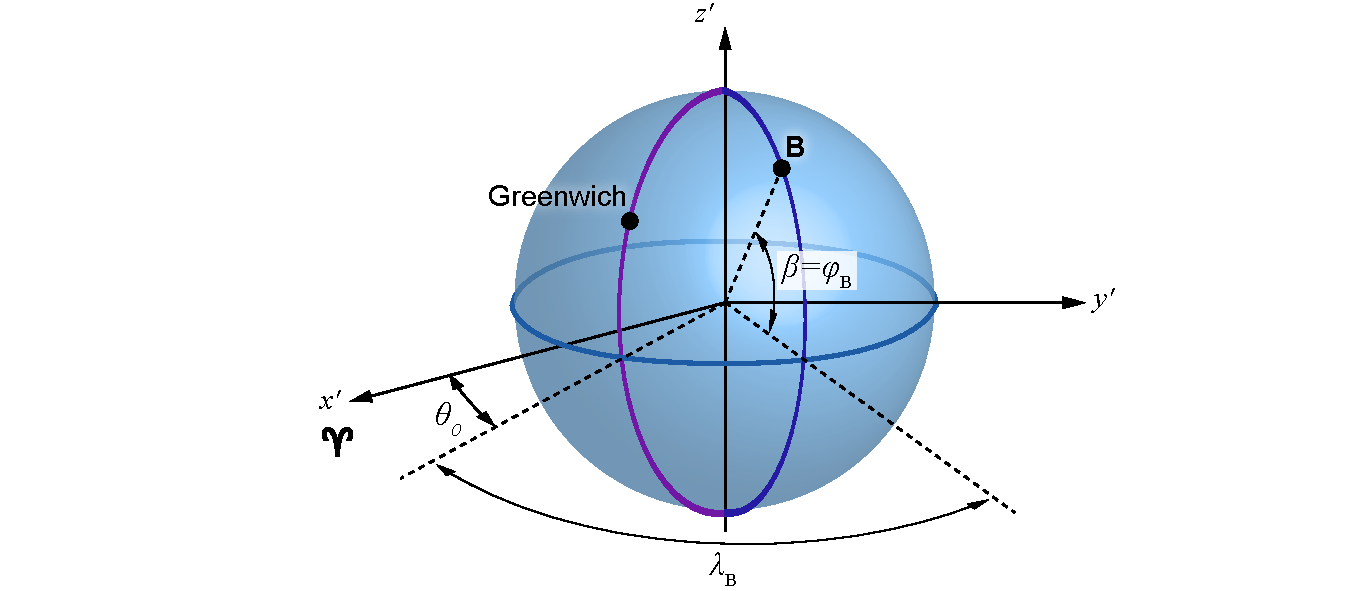
\includegraphics[width=\textwidth]{VenustransitKS.pdf}%
	\caption[Koordinatensystem des Beobachters beim Venustransit.]{Koordinatensystem ($x'$-$y'$-$z'$) des Beobachters beim Venustransit}%  
	\label{abb:hm_venustransit_lsg_2a}%
\end{figure}
	\item F�r die Koordinaten $\vec{r}'$ rechnen wir die geographischen Koordinaten $\varphi_\text{B}$, $\lambda_\text{B}$ eines Beobachters B in geozentrisch-�quatoriale Koordinaten um, wobei die Abplattung der Erde vernachl�ssigt wird und deshalb $\beta\!=\!\varphi_\text{B}$ ist.
          Damit gilt 
\begin{equation}
\vec{r}' = \lk\begin{matrix} x' \\ y' \\ z'\end{matrix}\rk = \mathbb{R}_\text{\earth}\,\lk\begin{matrix} \cos\beta\cos(\theta+\lambda_\text{B})\\ \cos\beta\sin(\theta + \lambda_\text{B})\\ \sin\beta \end{matrix}\rk ~~.
\label{eq:hm_venustr_d_2}
\end{equation}
\end{enumerate}	
	\begin{figure}[H]
	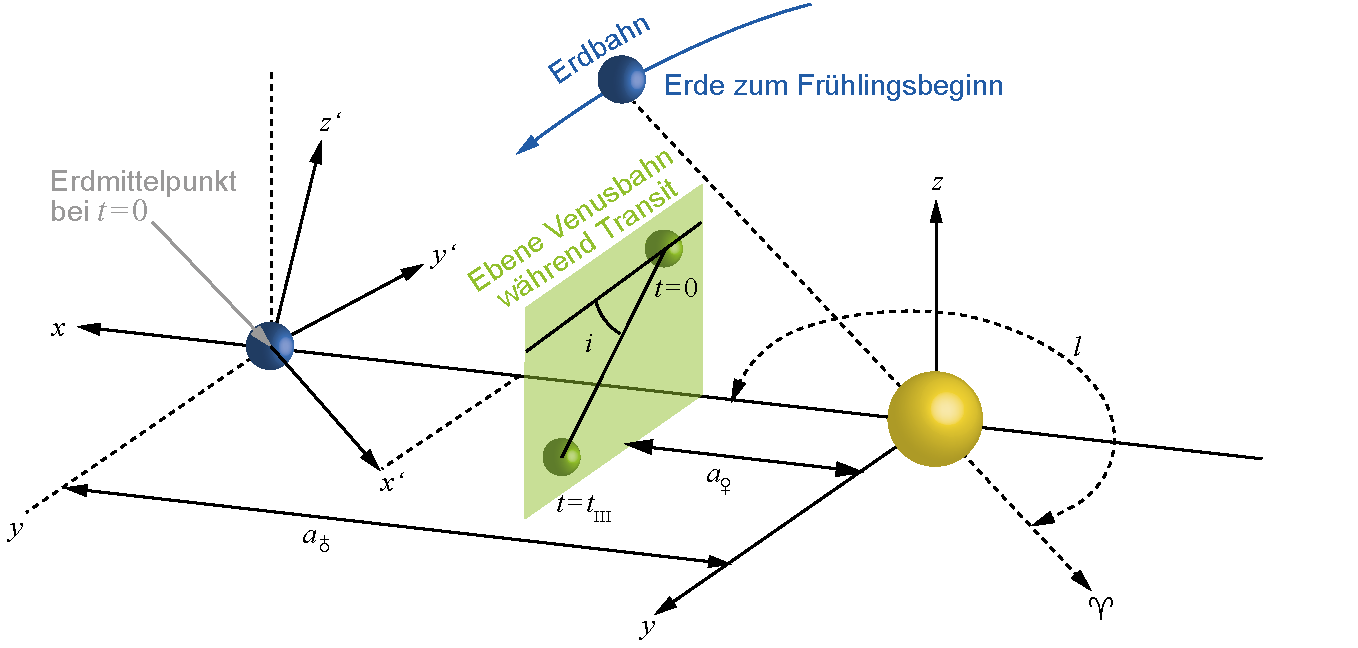
\includegraphics[width=\textwidth]{VenustransitHelioKS.pdf}%
	\caption[Beziehungen der Koordinatensysteme beim Venustransit.]{Beziehung des heliozentrischen Koordinatensystems ($x$, $y$, $z$) und des Koordinatensystems des Beobachters ($x'$, $y'$, $z'$) beim Venustransit}% 
	\label{abb:hm_venustransit_lsg_2b}%
	\end{figure}
	
	\item Das HE-KOS, welches f�r die Beschreibung der Planetenbewegung das geeignete ist.
          Bei diesem zeige die $x$-Achse nicht zum Fr�hlingspunkt, sondern zum Mittentransitzeitpunkt genau zum Erdmittelpunkt.
	\item Die Beziehung zwischen den kartesischen Koordinaten beider KOS ergibt sich nach \figref{hm_venustransit_lsg_2b} gem��:
	\begin{enumerate}[1.] 
	\item Translation
\begin{align}
	\vec{r} &= \mathbb{R}_z(-l)\,\mathbb{R}_y(-\epsilon)\,\vec{r}' + \vec{r}_\text{\earth\astrosun} \nonumber\\
	\smallskip
	\lk\begin{matrix} x \\ y \\ z \end{matrix}\rk &= \lk\begin{matrix} \cos l & \sin l & 0 \\ -\sin l & \cos l & 0 \\ 0 & 0 & 1\end{matrix}\rk \lk\begin{matrix} 1 & 0 & 0 \\ 0 & \cos\epsilon & \sin\epsilon \\ 0 & -\sin\epsilon & \cos\epsilon \end{matrix}\rk \lk\begin{matrix} x' \\ y' \\ z' \end{matrix}\rk + \lk\begin{matrix} a_\text{\earth} \\ 0 \\ 0 \end{matrix}\rk ~~. \label{eq:hm_venustr_d_1}
\end{align}
\item W�hrend der halben Dauer des Transits bewegt sich die Erde mit ihrer Winkelgeschwindigkeit $\omega_\text{\earth}$ weiter um die Sonne.
  Wir nehmend etwas vereinfachend an, dass diese Bewegung in der betrachtet kurzen Zeitspanne nur entlang der $y$-Achse erfolgt.
  D.\,h. wir haben 
\begin{equation}
\Delta \vec{r} = \lk\begin{matrix} 0 \\ \omega_\text{\earth}t \\ 0 \end{matrix}\rk ~~.
\label{eq:hm_venustr_d_4}
\end{equation}
Addiert man \eqref{eq:hm_venustr_d_4} und \eqref{eq:hm_venustr_d_1}, erh�lt man mit \eqref{eq:hm_venustr_d_2} und \eqref{eq:hm_venustr_d_3} f�r $\vec{r}'$ die Koordinaten des Beobachters zu einem beliebigen Zeitpunkt $t$ w�hrend des Transits.
\end{enumerate}
\end{enumerate}
\begin{figure}[H]
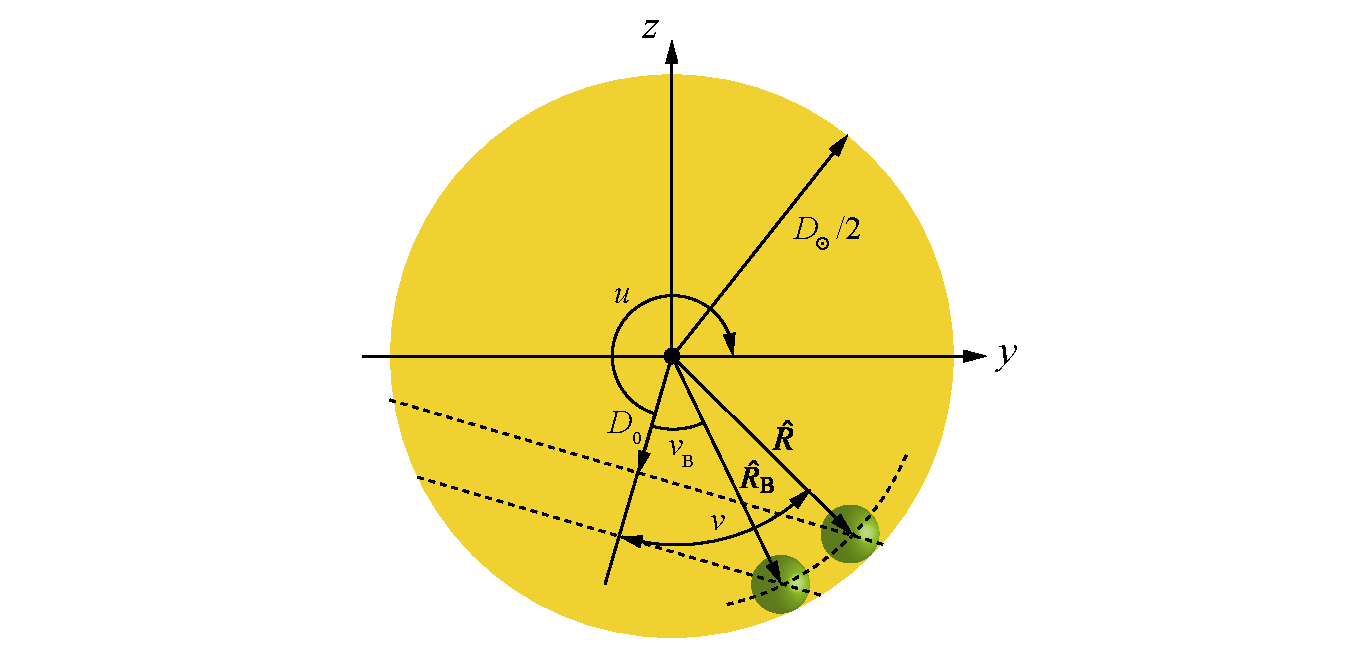
\includegraphics[width=\textwidth]{VenustransitGeometrie.pdf}%
\caption{Geometrie des Venustransits}%
\label{abb:hm_venustransit_lsg_3}%
\end{figure}

Wir betrachten nun als angenommener Beobachter im Erdmittelpunkt die Position der Venusprojektion vor der \anf{Sonnenscheibe} in \figref{hm_venustransit_lsg_3}.
Dabei m�ssen wir uns noch einmal klarmachen, dass zu jedem Zeitpunkt des Transits Erdmittelpunkt, Venusmittelpunkt und der Mittelpunkt des Venus-Projektionsscheibchens auf der Sonne auf einer Linie liegen.
F�r die Projektionsposition $\vec{r}_\text{P,0}$ (Mitte des Transits $t\!=\!0$) ergibt sich dann f�r die Position der Venus im $x,y,z$-KOS:
\begin{equation}
\gamma \lk \vec{r}_\text{\venus,0} - \vec{r}_\text{P,0} \rk =  \lk \vec{r}_\text{\earth,0} - \vec{r}_\text{P,0}\rk ~,
\label{eq:hm_venustr_d_5}
\end{equation}
worin $\gamma = a_\text{\earth}/a_\text{\venus}$ ist und 
\begin{equation*}
\vec{r}_\text{\earth,0} = \lk\begin{matrix} a_\text{\earth} \\ 0 \\ 0\end{matrix}\rk ~~\text{und}~~ \vec{r}_\text{P,0} = \lk\begin{matrix} 0 \\ D_0\cos u \\ D_0\sin u\end{matrix}\rk
\end{equation*}
jeweils die Positionen des Erdmittelpunktes und die Mitte des Projektionsscheibchens zum Transitmittenzeitpunkt sind.
F�r einen sp�teren Zeitpunkt $t$, z.\,B. dem Zeitpunkt des sogenannten 3. Kontakts $t_\text{III}$ gilt analog
\begin{equation}
\gamma \lk \vec{r}_\text{\venus,III} - \vec{r}_\text{P,III} \rk = \lk \vec{r}_\text{\earth,III} - \vec{r}_\text{P,III} \rk ~,
\label{eq:hm_venustr_d_6}
\end{equation}	
worin
\begin{equation*}
\vec{r}_\text{P,III} = \lk\begin{matrix} 0 \\ \hat{R}\cos(u+v) \\ \hat{R}\sin(u+v)\end{matrix}\rk ~~\text{mit}~~ \hat{R} = \frac{D_\text{\astrosun}}{2} - R_\text{P} ~~.
\end{equation*}	
Hierin ist $R_\text{P}$ der Radius des Projektionsscheibchens auf der Sonne und $D_\text{\astrosun}$ der Durchmesser der Sonne, jeweils in Winkelma�en angegeben.
F�r die Koordinaten $\vec{r}_\text{\venus,III}$ und $\vec{r}_\text{\earth,III}$ m�ssen wir die planetare Bewegung ber�cksichtigen (\figref{hm_venustransit_lsg_2b}), so dass dann folgt:
\begin{align}
	\vec{r}_\text{\earth,III} &= \lk\begin{matrix} a_\text{\earth} \\ \omega_\text{\earth} t_\text{III} \\ 0\end{matrix}\rk ~~, \nonumber\\
	\vec{r}_\text{\venus,III} &= \vec{r}_\text{\venus,0} + a_\text{\venus} \omega_\text{\venus} t_\text{III}\,\lk\begin{matrix} 0 \\ \cos i \\ -\sin i\end{matrix}\rk ~~. \label{eq:hm_venustr_d_7}
\end{align}	
Darin haben wir die Bewegung der Erde entlang der Richtung der $y$-Achse und die der Venus in der $y,z$-Ebene angenommen.
Die Bahnneigung der Venus gegen�ber der Ekliptik ist damit ber�cksichtigt, $\vec{r}_\text{\venus,0}$ ist durch \ref{eq:hm_venustr_d_5} gegeben.
Mit \eqref{eq:hm_venustr_d_5} bis \eqref{eq:hm_venustr_d_7} haben wir den Transit nun vollst�ndig f�r einen \anf{hypothetischen} Beobachter im Erdmittelpunkt beschrieben.
Wir wollen jetzt die Transitzeit bzw. die Zeit des 3. Kontakts bestimmen.
Wir erhalten aus der $y$-Komponente der Gleichung \eqref{eq:hm_venustr_d_6}
\begin{equation}
\sin u = \frac{a_\text{\venus} (\omega_\text{\earth} - \omega_\text{\venus}\cos i) }{(a_\text{\earth} - a_\text{\venus})\,\sqrt{\hat{R}^2 - D_0^2}}\,t_\text{III}
\label{eq:hm_venustr_d_8}
\end{equation}
und analog f�r die $z$-Komponente
\begin{equation}
\cos u = \frac{a_\text{\venus} \omega_{\venus} \sin i}{(a_\text{\earth} - a_\text{\venus})\,\sqrt{\hat{R}^2 - D_0^2}}\,t_\text{III} ~~.
\label{eq:hm_venustr_d_9}
\end{equation}	
Wegen $\cos^2 u + \sin^2 u\!=\! 1$ folgt aus \eqref{eq:hm_venustr_d_8} und \eqref{eq:hm_venustr_d_9}
\begin{equation*}
t_\text{III} = \lk \frac{a_\text{\earth}}{a_\text{\venus}} - 1 \rk\,\sqrt{\frac{\hat{R}^2 - D_0^2}{\omega_\text{\venus}^2 + \omega_\text{\earth}^2 - 2\omega_\text{\venus} \omega_\text{\earth} \cos i}} ~~.
\end{equation*}	
Man erkennt, dass f�r die im Beispiel \ref{bsp:venustransit} gemachte N�herung der koplanaren Bahnen sich tats�chlich die gesamte Transitzeit n�herungsweise zu	
\begin{equation*}
T_\text{TR} = 2t_\text{III} \approx (\gamma -1)\,\lk\frac{l_\text{s}}{\omega_\text{\venus} - \omega_\text{\earth}}\rk
\end{equation*}
ergibt.
Jetzt gehen wir vom Erdmittelpunkt zu einem Beobachter auf der Erdoberfl�che bei $(\varphi_\text{B},\lambda_\text{B})$ �ber.
Wir wissen aus der Geometrie, dass dessen beobachtete Zeit des 3. Kontakts $t_\text{III}^\text{(B)}\!\neq\! t_\text{III}$ ist.
Ebenso hat f�r ihn das Bild der Venus auf der Sonne bei $t\!=\!t_\text{III}^\text{(B)}$ andere Koordinaten als f�r den gedachten Beobachter im Erdmittelpunkt.
\begin{equation}
\vec{r}_\text{P,III}^\text{(B)} = \lk\begin{matrix} 0 \\ y_\text{P} \\ z_\text{P}\end{matrix}\rk ~~\text{mit}~~ \hat{R}_\text{B} = \hat{R} = \sqrt{y_\text{P}^2 + z_\text{P}^2} ~~.
 \label{eq:hm_venustr_d_10}
\end{equation}
Die Position des Beobachters auf der Erdoberfl�che zum Zeitpunkt $t\!=\!t_\text{III}^\text{(B)}$ ist demnach durch
\begin{equation}
\vec{r}_\text{\earth,III}^\text{(B)} = \lk \begin{matrix} x^\text{(B)} \\ y^\text{(B)} \\ z^\text{(B)} \end{matrix} \rk + \lk \begin{matrix} 0 \\ \omega_\text{\earth}t_\text{III}^\text{(B)} \\ 0 \end{matrix}\rk ~~.
\label{eq:hm_venustr_d_11}
\end{equation}
gegeben.
Die Position der Venus zu diesem Zeitpunkt ergibt sich aus \eqref{eq:hm_venustr_d_7} zu
\begin{equation}
\gamma \lk \vec{r}_\text{\venus,III}^\text{(B)} - \vec{r}_\text{\venus,0}^\text{(B)} \rk = \omega_\text{\venus} t_\text{III}^\text{(B)}\,\lk\begin{matrix} 0 \\ \cos i \\ -\sin i \end{matrix}\rk ~~.
\label{eq:hm_venustr_d_12}
\end{equation}
Der Vektor $\vec{r}_\text{\venus,III}^\text{(B)} - \vec{r}_\text{P,III}^\text{(B)}$ muss wiederum ein konstantes Vielfaches $k$ des Vektors $\vec{r}_\text{\earth,III}^\text{(B)} - \vec{r}_\text{P,III}^\text{(B)}$ sein, wie man sich leicht geometrisch klarmachen kann.
Wir erhalten aus der $x$-Komponente $k\!=\!a_\text{\venus}/x^\text{(B)}$, worin $x^\text{(B)}$ die Koordinate der Beobachterposition im kartesischen $x,y,z$ KOS zur Zeit $t_\text{III}^\text{(B)}$ ist.
Damit f�gen wir eine messbare L�ngendimension in das Gleichungssystem ein.
Analog erh�lt man f�r die $y$- und $z$-Komponenten von \eqref{eq:hm_venustr_d_10}
\begin{align*}
	y_\text{P} &= M + Nt_\text{III}^\text{(B)}~~,\\
	z_\text{P} &= P + Qt_\text{III}^\text{(B)}
\end{align*}
mit
\begin{align}
	M &= \frac{(\gamma-1)x^\text{(B)}\,D_0\cos u - y^\text{(B)}}{x^\text{(B)}/a_\text{\venus} - 1} ~~, \label{eq:hm_venustr_d_13} \\
	N &= \frac{x^\text{(B)}\omega_\text{\venus} \,\cos i - \omega_\text{\earth}}{x^\text{(B)}/a_\text{\venus} - 1} ~~, \nonumber\\
	P &=  \frac{(\gamma-1)x^\text{(B)}\,D_0\sin u - z^\text{(B)}}{x^\text{(B)}/a_\text{\venus} - 1} ~~, \nonumber \\
	Q &= \frac{x^\text{(B)} \omega_\text{\venus}\,\sin i}{x^\text{(B)}/a_\text{\venus} - 1} ~~. \nonumber
\end{align}
Wegen $y_\text{P}^2 + z_\text{P}^2\!=\!\hat{R}^2$ folgen schlie�lich die Relationen
\begin{align}
	\hat{R}^2 &= \lk M + Nt_\text{III}^\text{(B)}\rk^2 + \lk P - Qt_\text{III}^\text{(B)}\rk^2 ~~, \label{eq:hm_venustr_d_14} \\
	R^2 &= M^2 + 2NMt_\text{III} + N^2 t_\text{III}^2 + P^2 - 2PQt_\text{III} + Q t_\text{III}^2  ~~,\nonumber \\
	0 &= t_\text{III}^2 \lk N^2 + Q^2 \rk^2 + 2t_\text{III} (MN - PQ) + M^2 + P^2 - \hat{R}^2  ~~,\nonumber\\
	t_\text{III}^\text{(B)} &= -(MN - PQ) + \sqrt{(MN - PQ)^2 + \hat{R} - M^2 - P^2}  ~~.\nonumber
\end{align}
Damit hat man f�r einen Beobachter auf der geographischen Position $\varphi_\text{B},\lambda_\text{B}$ die Zeitdifferenz $t_\text{III}^\text{(B)} - t_\text{III}$ bei der Beobachtung des 3. Kontakts gegen�ber einem hypothetischen Beobachter im Erdmittelpunkt erhalten.
Hat man zwei Beobachter an zwei Orten, so kann man den hypothetischen Beobachter im Erdmittelpunkt eliminieren und betrachtet nur die Messungen der beiden Beobachter auf der Erdoberfl�che.
In $M$, $N$, $P$ und $Q$ sind mit Ausnahme von $a_\text{\venus}$ alle anderen Gr��en bekannt, also $D_0$, $u$, $\hat{R}$, $\omega_\text{\venus}$, $\omega_\text{\earth}$, $\gamma$ und $i$.
Man kann daher �ber einen Fit an $t_\text{III}^\text{(B)}(a_\text{\venus})$ f�r die Zeitdifferenz zweier Beobachtungssituationen den Abstand der Venus bestimmen und �ber das 3. Keplergesetz die Astronomische Einheit berechnen.\\
Sehr instruktiv ist eine "`Vorw�rtsrechnung"', d.h. eine Berechnung der relativen geozentrisch-�quatorialen Koordinaten von Sonne und Venus oder der entsprechenden topographisch-horizontalen Koordinaten (Achtung: hier wirklich topographische Koordinaten verwenden !) mit den heute verf�gbaren Daten aus der St�rungsrechnung.
Siehe auch Zusatzaufgabe \ref{prob:hm_Zusatz_VenusTransit_Vorwaerts}.
Ergebnisse daraus sind im hier f�r den Venustransit von 2004 angegeben (\mscr~\mlhmref{VenusTransit01.m} und \mlhmref{VenusTransit02.m}:). \\
\vspace{0.5 cm}
\begin{tabular}{L{4cm}R{2cm}R{2cm}}
\hline\noalign{\smallskip}
Ort & $t_\text{III}^\text{(B)} - t_\text{III}$ (berechnet) & beobachtet \\
\noalign{\smallskip}\svhline\noalign{\smallskip}
Oberkochen & $-1\:\text{min}\,12\:\text{s}$ & $-1\:\text{min}\,11\:\text{s}$ \\
Troms� & $-1\:\text{min}\,12\:\text{s}$ & \\
Canberra   &  $6\:\text{min}\,12\:\text{s}$ & \\
\end{tabular} 
\vspace{1 cm}
\\
Bemerkungen:
\begin{itemize}
	\item Bemerkung 1\\
Will man die Methode f�r den Transit an nur einem Standort benutzen, so muss man \eqref{eq:hm_venustr_d_14} etwas modifizieren.
Es ist relativ einsichtig, dass die Koordinaten $x^\text{(B)}$, $y^\text{(B)}$ und $z^\text{(B)}$ von $M$, $N$, $P$ und $Q$ von $t_\text{III}^\text{(B)}$ abh�ngen und zu einer bestimmten Zeit berechnet werden m�ssen (\ldots Unterschied zwischen UT und ET beachten!).
Die Gleichungen \eqref{eq:hm_venustr_d_14} sind dann vom Typ
\begin{equation*}
t_\text{III}^\text{(B)} = f(t_\text{III}^\text{(B)},a_\text{\venus})~~,
\end{equation*}
die numerisch nach $a_\text{\venus}$ gel�st werden kann.\\
\item Bemerkung 2\\
Eine v�llig analoge und gleichzeitig sehr instruktive Betrachtung kann man anstellen, wenn man berechnet wie der Venusschatten die Erde trifft.
Diese Methode ist ausf�hrlich in \cite{Backhaus2012} mit Daten f�r den Venustransit von 2012 beschrieben.\\
\item Bemerkung 3\\
Mit zuk�nftigen Marsmissionen wird man nicht bis zum n�chsten Venustransit warten m�ssen, um wieder einen Planeten vor der Sonne vor�berziehen zu sehen.
Nat�rlich gelten alle bisher gemachten �berlegungen auch f�r einen Beobachter auf dem Mars.
Dieser kann dann nat�rlich auch beobachten, wie unsere Erde und ihr Mond vor der Sonne vor�berziehen.
Das letzte Ereignis dieser Art war am 11. Mai 1984 und das n�chste ist am 10.November 2084.
Wir sind aber nicht sicher, ob bereits jetzt Anmeldungen entgegen genommen werden.
Wir empfehlen das mit dem \mscr~\mlhmref{InnerePlaneten.m} \bzw \mlhmref{VenusTransit01.m} zu �berpr�fen.
F�r eine genauere Rechnung der Transitzeiten benutzen Sie die Koordinatenberechnungen nach der St�rungstheorie, d.h. die Funktionen \mlhmiref{SonneExakt.m} und \mlhmiref{MarsExakt.m}.
Siehe auch Zusatzaufgabe \ref{prob:hm_Zusatz_ErdeTransit_from_Mars}.\\
\end{itemize}
\end{enumerate}
\medskip \end{sol}
\textcolor{blue} {$\rightarrow$ zur} \probref{hm_venus_2004_2012}.\\
\noindent\rule[1ex]{\textwidth}{0.5pt} \newpage


%-----------------------------------------------------------------------------------------------------------

\begin{sol}{prob:hm_jupiterbedeckung_venus} \label{lsg:hm_jupiterbedeckung_venus} %�bung19
\textbf{Jupiterbedeckung durch die Venus am 22.11.2065} \\ \\
Die Rechnungen sind im Detail in \mlhmref{PlanetenbahnenKepler.m} ausgef�hrt. \\

\begin{figure}[H]
\begin{minipage}{\textwidth}
\leftfigure{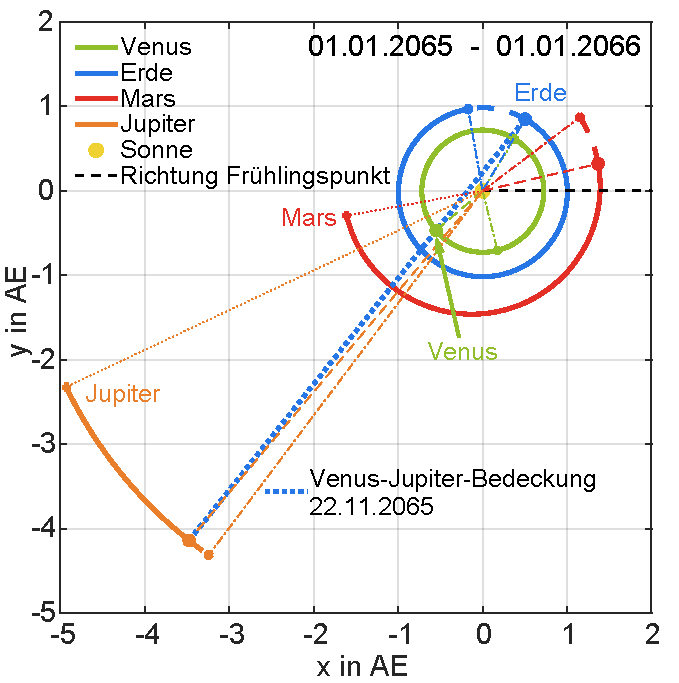
\includegraphics[width=0.5\textwidth]{JupiterBedeckung.pdf}}
\hspace{\fill}
\rightfigure{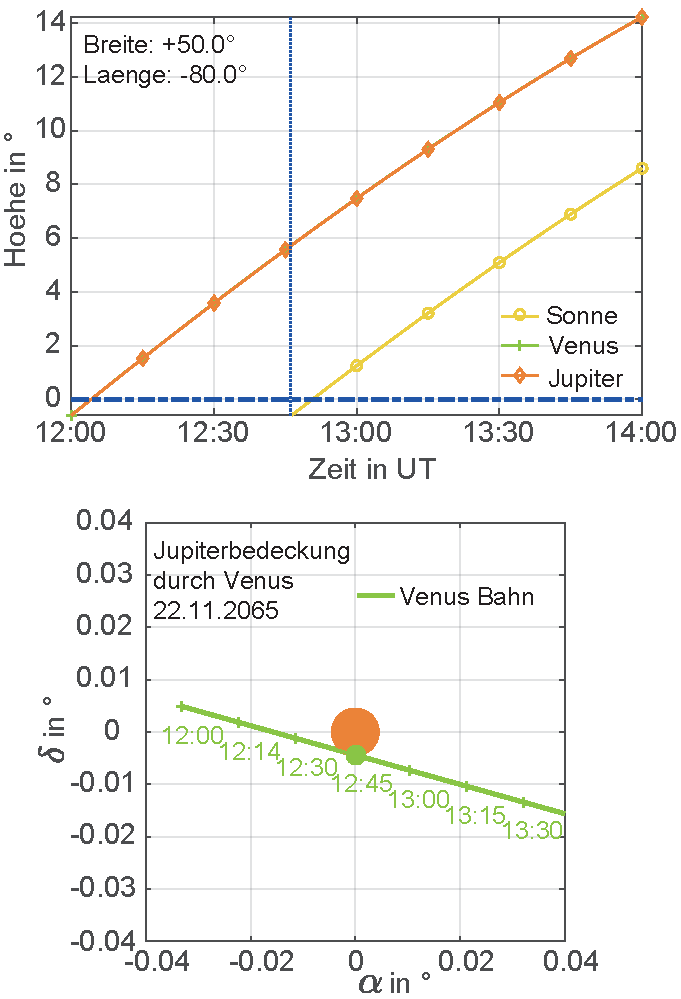
\includegraphics[width=0.5\textwidth]{JupiterVenus.pdf}}
\leftcaption{Konstellation der Planeten am 22.11.2065}\label{abb:hm_JupiterBedeckung_lsg}
\rightcaption{Jupiterbedeckung durch Venus am 22.11.2065}\label{abb:hm_JupiterVenus_lsg}
\end{minipage}
\end{figure}

Aufgrund der erforderlichen Pr�zision wurden die im \matlab{} Programm die hinterlegten Routinen \mlhmiref{VenusExakt.m} und \mlhmiref{JupiterExakt.m} f�r die Berechnung der Planetenpositionen benutzt.
Diese auf den Reihenentwicklungen der St�rungstheorie entwickelten Routinen wurden \cite{Montenbruck1999} entnommen und liefern Genauigkeiten von besser als 10 Bogensekunden �ber den Zeitraum von ca. 50 Jahren.\\
Leider ist die Bedeckung des Jupiters durch die Venus nicht ganz vollst�ndig und noch dazu sehr ung�nstig zu beobachten, da beide Planeten einen relativ geringen Winkelabstand zur Sonne haben.
Am ehesten hat man eine Chance in Nordamerika.

\medskip \end{sol}
\textcolor{blue} {$\rightarrow$ zur} \probref{hm_jupiterbedeckung_venus}.\\
\noindent\rule[1ex]{\textwidth}{0.5pt} \newpage


%%%-----------------------------------------------------------------------------------------------------------

\subsection{�bungen zu Himmelsbeobachtungen von anderen Planeten aus}

\medskip

%-----------------------------------------------------------------------------------------------------------

\begin{sol}{prob:hm_erdaufgang_von_mond} \label{lsg:hm_erdaufgang_von_mond} %�bung20
\textbf{Kann man einen Erdaufgang vom Mond aus sehen?} \\ \\
Als erste Reaktion w�rde man sagen, dass auf dem Mond keine Erdauf- bzw. unterg�nge beobachtet werden k�nnen, da ein Beoabachter auf der Mondvorderseite wegen der gebundenen Rotation (\vgl auch L�sung \ref{lsg:hm_erdrotation}) immer die Erde sieht, wenn auch in verschiedenen Beleuchtungsphasen, so wie wir den Mond sehen.
Diese Behauptung gilt aber nur f�r eine exakt kreisf�rmige Bahn.
Auf Grund der relativ starken Elliptizit�t der Mondbahn und der daraus folgenden unterschiedlichen Geschwindigkeiten, zeigt der Mond der Erde immer ein leicht anderes Antlitz.
Er \anf{sch�ttelt} sozusagen den Kopf (Wir hoffen, dass dies nicht als Missfallen gegen�ber den hier gemachten physikalischen Betrachtungen gedeutet werden muss.).
Dieser Effekt ist schon seit dem Mittelalter als \emph{Libration} bekannt.
Die Libration kann einfach abgesch�tzt werden, indem man das Erde-Mond-System als ZKP betrachtet und die maximale Differenz von wahrer und mittlerer Anomalie berechnet.\\
Mit den Werten f�r die Exzentrizit�t $e_\text{Mond}\!=\!0.0549$ ergibt sich mit den ersten Termen der Mittelpunktsgleichung \eqref{eq:hm_mpglg_nu-M}, wenn f�r die mittlere Anomalie $M_\text{Mond} (t)\!= \!134.96\degree + 13.06\degree \, t \; \text{in} [\degree/\text{d}$] der Wert $90\degree$ oder $270\degree$ eingesetzt wird (der Zeitpunkt $t$ spielt f�r uns jetzt keine Rolle):
\begin{equation*}
	\delta \,l_\text{lib} = C_\text{Mond,max} \approx \upsilon - M_\text{Mond,max} = 2e_\text{Mond} + \frac{5}{5}e_\text{Mond}^3\! + \ldots \approx 0.11 \approx 6.3\degree ~~.
\end{equation*}
Die tats�chliche Libration betr�gt etwa $7.9\degree$.
Der Unterschied von ca. $1.6\degree$ kommt durch den zus�tzlichen Einfluss der Sonne zustande.
Die Erde erscheint vom Mond betrachtet unter einem Winkel 
\begin{equation*}
	2\alpha = \arctan \lk\frac{R_{\earth}}{a_{{\earth}\text{Mond}}} \rk \approx 1.9\degree ~~, 
\end{equation*}
was deutlich kleiner ist als $\delta l_\text{lib}$.
Man kann also vom Mond aus den Erdaufgang sehen, vorausgesetzt man befindet sich in den \anf{Randbereichen} des Mondes (bei selenographische L�ngen um $90\degree$) oder in einem Raumschiff (\probref{hm_erdaufgang_von_apollo}).
Der Landeplatz von Apollo 11 war allerdings bei bei einer selenographischen Position von $0\degree$N und $23.5\degree$W (also nahe des Mond�quators), so dass Armstrong\indexp{Armstrong, Neil Alden} und Aldrin\indexp{Aldrin, Buzz} diese Beobachtung nicht verg�nnt war.
Abgesehen davon, waren sie nicht lang genug auf dem Mond, denn die Periode der Libration ist in etwa so lang wie der anomalistische Monat von ca. $27.5$ Tagen.
Man kommt also in den entsprechenden Bereichen nur einen Tag im Monat in den Genuss des Erdaufgangs.\\
\medskip \end{sol}
\textcolor{blue} {$\rightarrow$ zur} \probref{hm_erdaufgang_von_mond}.\\
\noindent\rule[1ex]{\textwidth}{0.5pt} \newpage

%-----------------------------------------------------------------------------------------------------------

\begin{sol}{prob:hm_erdaufgang_von_apollo}\label{lsg:hm_erdaufgang_von_apollo} %�bung21
\textbf{Earth Rise von Apollo 8} \\ \\
Wie man aus \figref{hm_EarthRise_calc} sieht, m�sste man das von Apollo 8 aufgenommene Bild eigentlich um $90\degree$ gegen den Uhrzeigersinn drehen, die Sonne kam von links.
Wenn man noch wei�, dass Apollo 8 zu dieser Zeit auf einer elliptischen Bahn war, deren Pericynthion (mondnaher Punkt) bei $\SI{112}{\kilo\metre}$ und deren Apocynthium (mondferner Punkt) bei $\SI{312}{\kilo\metre}$  lagen, sowie die Umlaufbahn um zwei Grad gegen den Mond�quator geneigt war, kann man auch relativ genau die Position des Raumschiffs berechnen (Zusatzaufgabe).  F�r Interessanten haben wir im \mscr{} \mlhmref{Apollo8LunarOrbit.m} die Bahn und den Zeitpunkt des Earth Rise Fotos mit den Daten des jPL berechnet und dargestellt.

\medskip \end{sol}

\begin{figure}[H]
\begin{minipage}{\textwidth}
\leftfigure{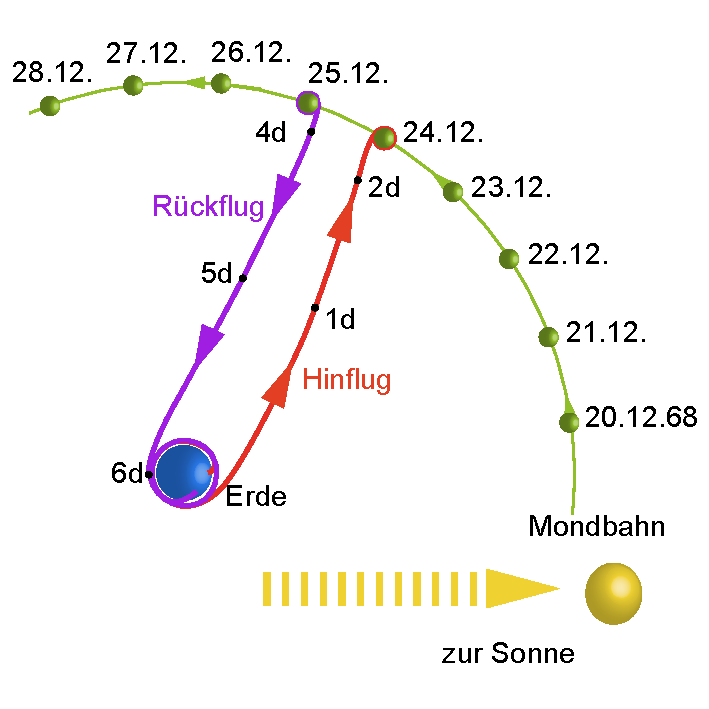
\includegraphics[width=0.5\textwidth]{Apollo8_Bahn.pdf}}
\hspace{\fill}
\rightfigure{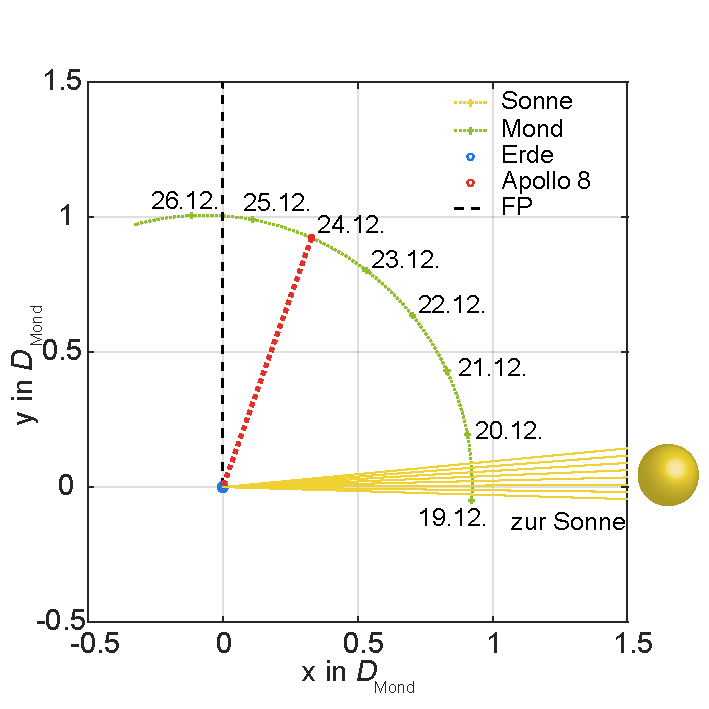
\includegraphics[width=0.5\textwidth]{KonstellationSEMA.pdf}}
\leftcaption[Bahn von Apollo 8.]{Bahn von Apollo 8. \\(Copyright NASA)}\label{abb:hm_Apollo8_Bahn}
\rightcaption[Konstellation von Sonne, Erde, Mond und Apollo 8 am 24.12.1968.]{Berechnete Konstellation von Sonne, Erde, Mond und Apollo 8 am 24.12.1968 um 16:38 UT} \label{abb:hm_EarthRise_calc}
\end{minipage}
\end{figure}
\textcolor{blue} {$\rightarrow$ zur} \probref{hm_erdaufgang_von_apollo}.\\
\noindent\rule[1ex]{\textwidth}{0.5pt} \newpage

%-----------------------------------------------------------------------------------------------------------

\begin{sol}{prob:hm_Analemma_Mars}\label{lsg:hm_Analemma_Mars} %�bung22
\textbf{Zeitgleichung und Analemmas auf anderen Planeten} \\

Wir wollen zun�chst eine sehr einfache Berechnung zeigen, die die Form der Analemmas richtig wider gibt, allerdings keine zeitliche Entwicklung zeigt, da die Kepler-Gleichung nicht gel�st wird.
Man startet dazu mit der exzentrischen Anomalie $E$ und betrachtet ein ganzes planetarisches Jahr, von dem man wei�, dass $E = 0 \ldots 360 \degree$ ist.
Mit Formel \eqref{eq:hm_nu(t)_alternativ}
\begin{equation*}
	\tan \lk \frac{\upsilon_\text{P}}{2} \rk = \sqrt{\frac{1+e_\text{P}}{1-e_\text{P}}}\,\tan\lk\frac{E}{2}\rk~
\end{equation*}
berechnet man die wahre Anomalie $\upsilon_\text{P} (E)$ des Planeten P.
Aus dieser bestimmt man �ber \eqref{eq:hm_ekl_laenge_erde1} und \eqref{eq:hm_lambda_S(T)} die L�ngen der wahren und mittleren Sonne
\begin{equation*}
L_\text{P,\astrosun} = \upsilon_\text{P} +  L_\text{P,Per}\,,~~~ L_\text{P,M} = M_\text{P} +  L_\text{P,Per} \,.
\end{equation*}
Dazu braucht man die planetozentrische L�nge des Perihels.
Das ist der Winkelabstand des Perihels vom planetaren Fr�hlingspunkt, der sich wiederum als Schnittpunkt der �quatorebene des Planeten mit der Bahnebene des Planeten ergibt.

	\begin{figure}[H]
	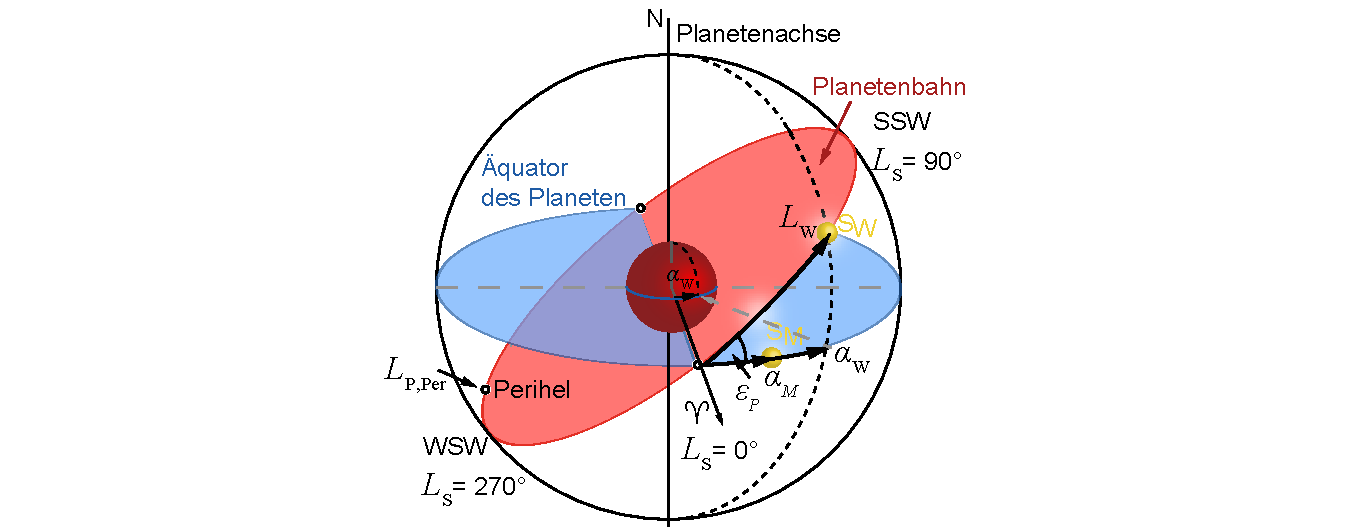
\includegraphics[width=0.8\textwidth]{ZGLGeometrie.pdf}%
	\caption{Ableitung der planetaren Sonnenkoordinaten}%
	\label{abb:hm_ZGLGeometrie_lsg}%
	\end{figure}

Wir betrachten dazu \figref{hm_ZGLGeometrie_lsg}, die der \figref{hm_wahre_sonne_geoz} aus \kap{hm_naeherungsformeln_sonne} f�r die Erde entspricht.
Wie dort dargestellt, geht es auch hier um die Anwendung von Gleichung \eqref{eq:hm_tau_ZGL_C}.
Hier m�ssen wir nun anstelle der ekliptikalen L�nge $\lambda_\text{\astrosun}$ und der geozentrischen Rektaszension $\alpha_\text{\astrosun}$ die planetozentrische L�nge $L_\text{P,\astrosun}$\index{L�nge!planetozentrische} und die planetozentrische Rektaszension \index{Rektaszension!planetozentrische} \index{Rektaszension!planetare} $\alpha_\text{P,\astrosun}$ verwenden.
Mit dem Begriff \emph{planetare} oder \emph{planetozentrische} Rektaszension ist analog zur "`normalen"' \emph{geozentrischen} Rektaszension ein Winkel gemeint, der entlang des planetaren �quators vom \emph{planetaren}(!) Fr�hlingspunkt zum Fusspunkt der wahren Sonne aus gemessen wird. 
Die (planetare) Rektaszension ergibt sich aus der entsprechenden Umrechnungsformel vom planeto-ekliptikalen System in das planeto-�quatoriale KOS (Tab. \ref{tab:hm_astro_KOS}):
\begin{equation*}
\tan\alpha_\text{P,\astrosun} = \cos\epsilon_\text{P} \, \tan{L_\text{P,\astrosun}} ~~\text{bzw.}~~~ \alpha_\text{P,M} = L_\text{P,M}~,
\end{equation*}
worin $\epsilon_\text{P}$ die Polneigung des jeweiligen Planeten relativ zu seiner Bahn ist.
Damit ergibt sich der Stundenwinkel nach \eqref{eq:hm_tau_ZGL_C} zu $\tau = \alpha_\text{M} - \alpha_\text{\astrosun}$.
Die Deklination der wahren Sonne berechnet sich ebenfalls aus Tabelle \ref{tab:hm_astro_KOS} zu:
\begin{equation*}
\sin\delta_\text{\astrosun} = \sin\epsilon_\text{P} \, \sin{L_\text{P,\astrosun}} ~, 
\end{equation*}
womit wir alle Berechnungsdaten f�r die Analemmas der Planeten haben.

\begin{figure}[H]
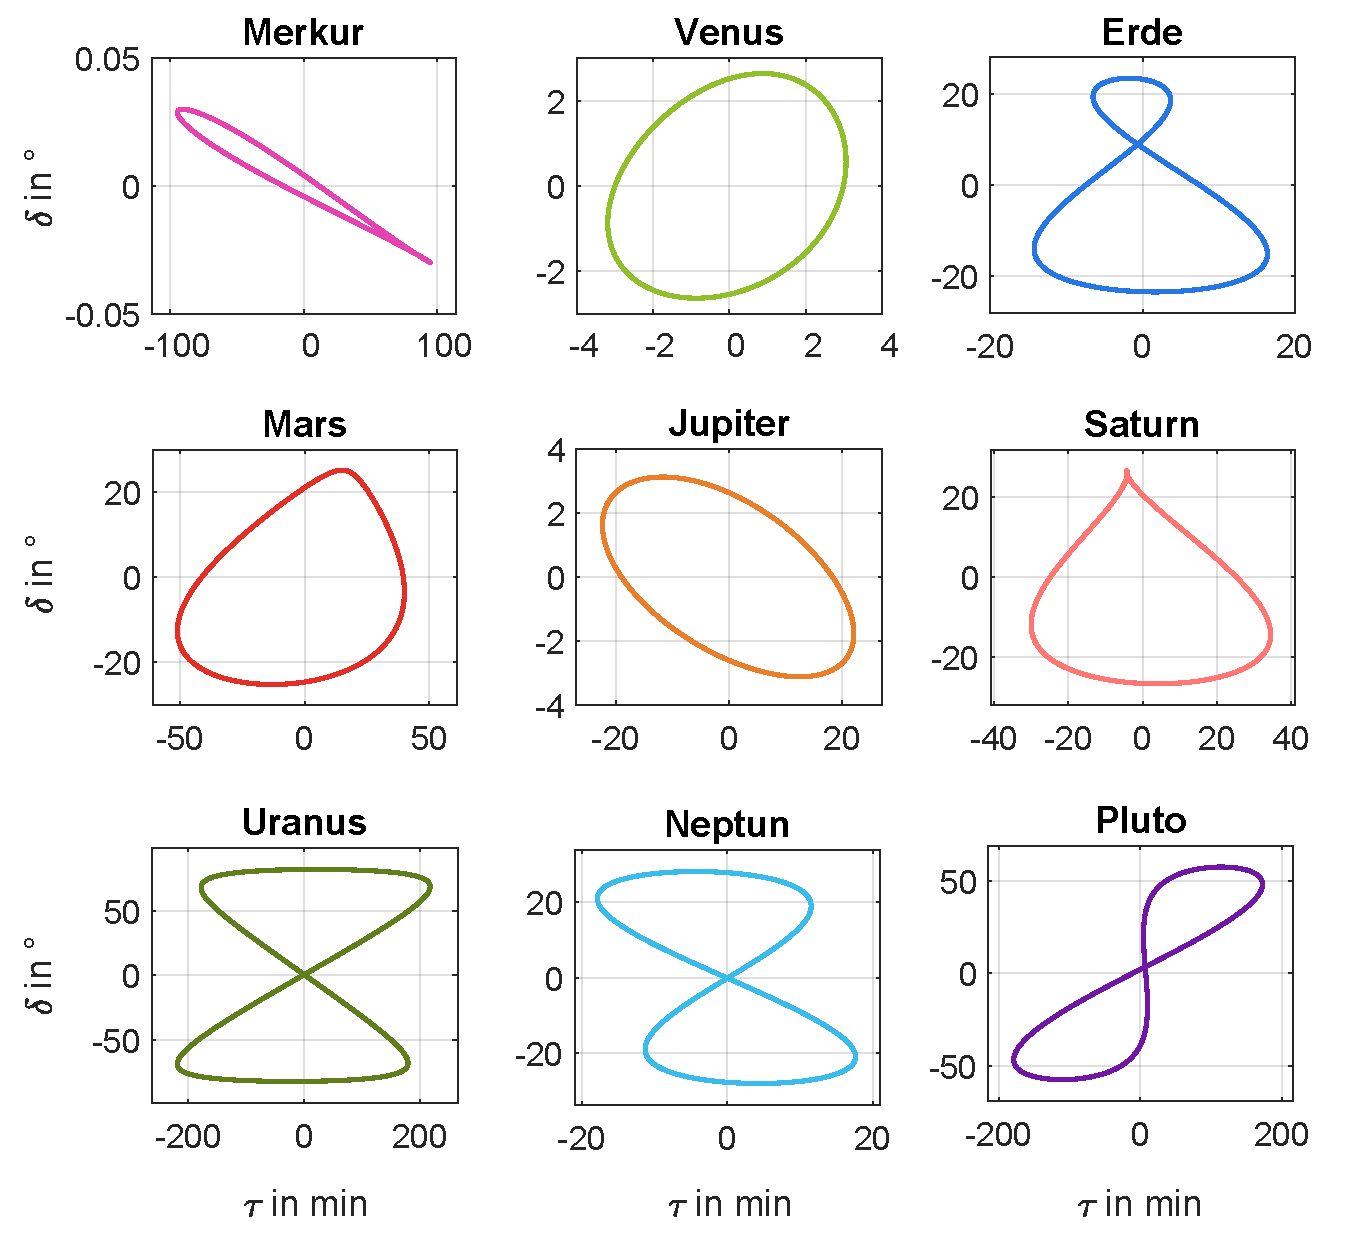
\includegraphics[width=\textwidth]{AnalemmaPlaneten.pdf}
\caption{Analemma f�r die Planeten Merkur bis Pluto.}\label{abb:hm_analemma_planeten_lsg}
\end{figure}
Details der Berechnung sind in \mlhmref{Analemma03.m} zu finden.
Das Ergebnis der Berechnung l�sst sich zusammenfassen, wobei wir den Index P f�r den Planeten weglassen, aber noch einmal darauf hinweisen, dass hier die $L_\text{Per}$ nicht den in Tabelle \ref{tab:hm_bahnparameter} gelisteten heliozentrisch-ekliptikalen L�ngen des Perihels entsprechen, sondern den planetozentrischen $L_\text{P,Per}$.
\begin{align*}
    \tau_\text{ZGL}(E) &= M + L_\text{Per} - \arctan\left\{\cos\epsilon\:\tan\left[L_\text{Per} +  2 \arctan\lk\sqrt{\frac{1+e}{1-e}} \tan\lk \frac{E}{2} \rk \rk \right] \right\} ~,\\
    \delta(E) &= \arcsin\left\{\sin\epsilon \sin\left[L_\text{Per} + 2 \arctan\lk \sqrt{\frac{1+e}{1-e}} \tan\lk \frac{E}{2} \rk \rk \right] \right\}
\end{align*}
Die entsprechenden Rechnungen haben wir im \mscr~\mlhmref{AnalemmaAnomalie.m} durchgef�hrt und sind in \figref{hm_analemma_planeten_lsg} gezeigt.
Wir geben die planetozentrischen L�ngen des Perihels ebenfalls im \mscr~an.
Wir sehen im Ergebnis, dass nur auf einigen Planeten  das Analemma als die von der Erde bekannten Figur der "`Acht"' erscheint, auf anderen Planeten kommt es wegen des unterschiedlichen Zusammenspiels der Parameter Achsneigung und Exzentrizit�t zu anderen Bildern.
Wenn einer der Bahnparameter dominiert, wie z.B. die Exzentrizit�t beim Mars, dann �hnelt das Analemma eher einer Tr�ne (siehe \figref{hm_analemma_planeten_lsg}), wenn hingegen die Achsneigung sehr klein ist, wie beim Jupiter (nur $3\degree$) wird die Figur �hnlich einer Ellipse.
Man beachte daher die ausgepr�gte Form und Breite bei Planetenbahnen mit gro�er Exzentrizit�t (Merkur, Mars, Saturn), die verschwindende Form der "`Acht"' bei geringer Polneigung (Merkur, Venus, Jupiter) bzw. das �berwiegen der Exzentrizit�t �ber die Polneigung (Mars, Saturn).\\
Wir wollen uns nun auch der Zeitgleichung zuwenden und m�ssen dazu die L�sung der Kepler-Gleichung f�r den jeweiligen Planeten ber�cksichtigen.
Wir skizzieren dazu zwei alternative Methoden. \\

\emph{Methode 1 (nach Allison\footnote{Die Rechnungen erfolgen analog den Betrachtungen in Kapitel \ref{kap:zeitgleichung} und sind in den \mscren zur �bung im Detail beschrieben. Wir verweisen ferner auf die Darstellungen in \cite{Allison2000} und \cite{Goddard2019}, in denen die Rechnungen ausf�hrlich f�r den Mars hergeleitet wurden. Wir haben in der �bung das Vorgehen f�r alle Planeten verallgemeinert.})}

Die Rotation des Planeten muss man zun�chst nicht ber�cksichtigen.
Man muss aber wiederum die Lage der Planetenbahn relativ zum planetaren �quator kennen oder m.a.W. die Richtung der Planetenrotationsachse relativ zu seiner Bahnebene.
Wir verweisen wieder auf die \figref{hm_ZGLGeometrie_lsg}, dann besteht die Aufgabe in Folgendem:
\begin{enumerate} 
	\item 	Es m�ssen die Keplerschen Elemente der Planetenbahn (bzw. der vom Planeten aus gesehenen Sonnenbahn) relativ zum planetaren �quator und Fr�hlingspunkt ausgedr�ckt werden.
          Bekannt sind dabei ja zun�chst nur die Bahnelemente bezogen auf die (Erd-)Ekliptik und den Erdfr�hlingspunkt.
          Halbachse und Exzentrizit�t �ndern sich nicht, ebenso bleibt die mittlere Anomalie unver�ndert.
          Die anderen Bahnelemente m�ssen jedoch transformiert werden.
	\item 	Mit der Inklination $i$, der L�nge des Knotens $\Omega$, dem Argument des Perihels $\omega$ und der Richtung der Rotationsachse des Planeten (deren Richtungswerte\footnote{Mit Richtung der Rotationsachse meinen wir die geozentrische Rektaszension und Deklination des Punktes an der Himmelskugel auf den die Rotationsachse zeigt.} $\alpha_0, \delta_0$ man aus der Literatur entnimmt) muss man nun die Lage des planetaren Fr�hlingspunktes (PFP) \index{Fr�hlingspunkt!planetarer} auf dem planetaren �quator berechnen (siehe \figref{hm_ZGLNullmeridian_lsg}) und daraus den Winkel $L_{\text{P,Per}}$ zwischen planetarem Fr�hlingspunkt und Perihelion der Planetenbahn.
	\item 	Am einfachsten geht das mittels Rotationsmatrizen f�r die kartesischen Vektoren normal zu den einzelnen Ebenen und entlang der jeweiligen Knotenlinien. 
	\item 	Mit diesen Gr��en kann dann die planetare Zeitgleichung, die der ekliptikalen ZGL nach \eqref{eq:hm_tau_ZGL_C} bzw. \eqref{eq:hm_tau_ZGL_C1} entspricht, berechnet werden:
		\[\tau_\text{ZGL, P} = (L_\text{P,\astrosun}-\alpha_\text{P,\astrosun}) + \mathcal{C} \\
	\]
	\item Mit der Deklination $\delta_\text{P,\astrosun}$, die wir aus der planetozentrischen L�nge der Sonne und der Achsneigung analog \eqref{eq:hm_alpha_s_delta_s} berechnen, erstellen wir dann das Analemma.
\end{enumerate}

\begin{figure}[H]
	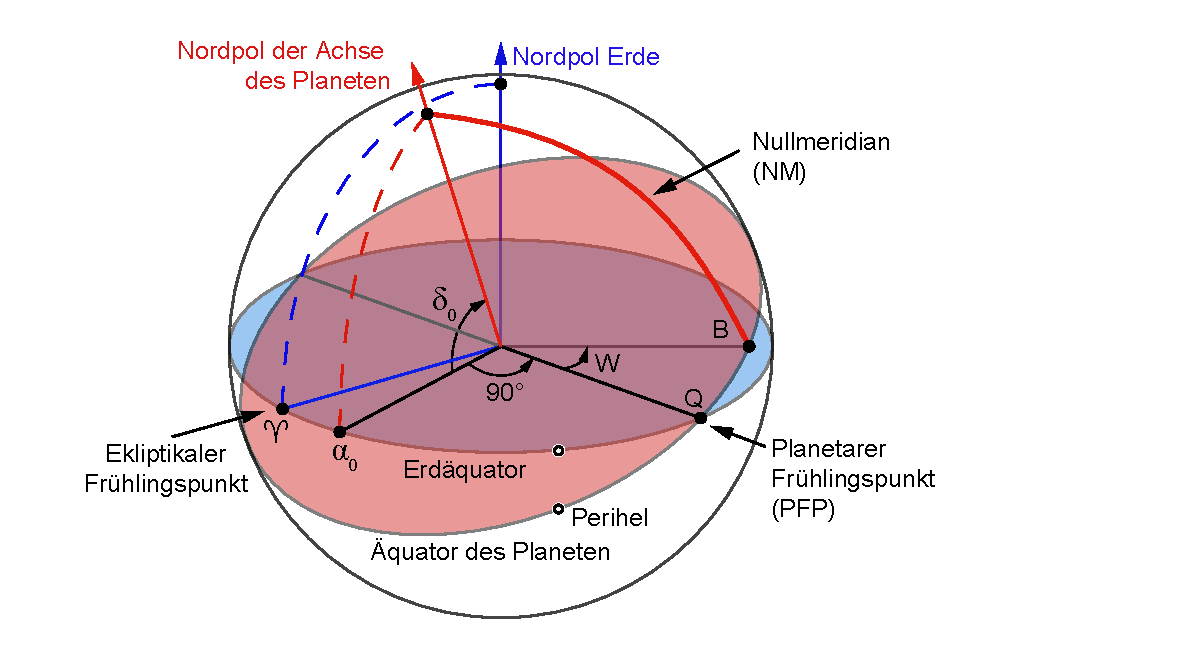
\includegraphics[width=\textwidth]{ZGLNullmeridian.pdf}%
	\caption[Planetarer Fr�hlingspunkt und Nullmeridian.]{Planetarer Fr�hlingspunkt (PFP) und Nullmeridian (NM).}%
	\label{abb:hm_ZGLNullmeridian_lsg}%
\end{figure}

Die entsprechenden Rechnungen haben wir im \mscr~\mlhmref{ZGLAnalemma.m} durchgef�hrt.

\begin{figure}[H]
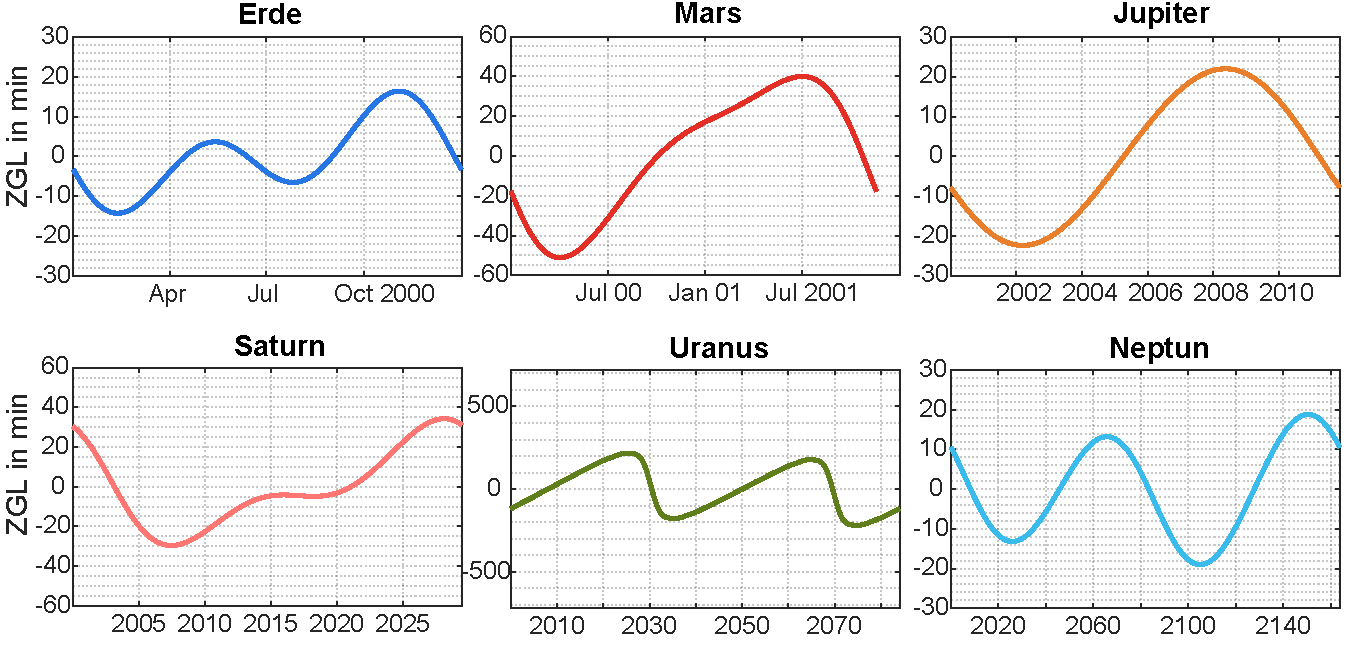
\includegraphics[width=\textwidth]{ZGLAnalemma.pdf}
\caption{Zeitgleichung f�r einige Planeten.}\label{abb:hm_zgl_planeten_lsg}
\end{figure}

Die Ergebnisse der Zeitgleichungsrechnung sind in \ref{abb:hm_zgl_planeten_lsg} dargestellt, die Analemmas stimmen erwartungsgem�� mit denen von \ref{abb:hm_analemma_planeten_lsg} �berein.
Wir wollen hier nochmals auf die Besonderheit des Uranus verweisen.
Der Uranus braucht etwa 84 Jahre, bis er die Sonne einmal umrundet hat.
Dabei dauert ein Tag auf dem Uranus nur 17 Stunden und 14 Minuten.
Da seine Polachse fast in der Bahnebene liegt rollt er quasi auf seiner Bahnebene um die Sonne, wobei f�r fast ein halbes Jahr der Nordpol, das andere Halbjahr der S�dpol zur Sonne zeigt.
Die ZGL und damit Jahreszeiten sind aus diesem Grund ziemlich "`verr�ckt"'.
Es bleibt auf dem Uranus im Sommer 42 Erden-Jahre lang st�ndig hell und wird dann abrupt dunkel.
Das Analemma zeigt das sehr sch�n.\\

\emph{Methode 2 (nach Montenbruck\footnote{Mit der Methode ist dann auch die Position jedes anderen Himmelsk�rpers im KOS des Planeten berechenbar. F�r Details verweisen wir auf \cite{Montenbruck1999, Haase2013}.})} 

Auch hier wollen wir die Methodik kurz skizzieren.
Man berechnet (numerisch) f�r einen Punkt auf der Oberfl�che des Planeten (gegeben durch die planetographischen Koordinaten $\varphi_\text{P}$ und $\lambda_\text{P}$) die planetare Rektaszension und Deklination der Sonne im planetozentrischem �quatorialsystem f�r den Verlauf eines tropischen Jahres.
Aus diesen Koordinaten lassen sich dann v�llig analog zur Erde bei Festlegung einer geeigneten Planeten-Nullzeit (z.B. Nullmeridian NM in \figref{hm_ZGLNullmeridian_lsg}) die Aufg�nge und Unterg�nge der Sonne und nat�rlich auch den Meridiandurchgang f�r jeden Ort $\varphi_\text{P}$, $\lambda_\text{P}$ des Planeten bestimmen.
Zusammengefasst ist das Vorgehen also wie folgt:
\begin{enumerate} 
	\item Ausgehend von der heliozentrischen Position des Planeten berechnet man die planetozentrischen Koordinaten $\alpha_\text{P,\astrosun}$  und $\delta_\text{P,\astrosun}$ der wahren Sonne im Verlauf eines tropischen Jahres.
	\item Die mittlere Sonne berechnen wir �ber die mittlere Anomalie.
          Alternativ k�nnten wir auch aus der Kenntnis der Rotationsperiode des Planeten eine Planetensternzeit $\theta_\text{P}$ berechnen, wobei sich die Zeitgleichung dann entweder �ber \eqref{eq:hm_tau_ZGL_C} bzw. $\tau_\text{ZGL} = \theta_\text{P} - \alpha_\text{P,\astrosun}$ berechnet. 
	\item Mit der Deklination $\delta_\text{P,\astrosun}$ aus der planetozentrischen Breite der wahren Sonne erstellen wir dann das Analemma.
\end{enumerate}

Die entsprechenden Rechnungen haben wir im \mscr~\mlhmref{ZGLAnalemmaKepler.m} bzw. f�r alle Planeten hinterlegt.
Auch hier stimmen die Analemmas erwartungsgem�� mit denen von \figref{hm_analemma_planeten_lsg} und die Zeitgleichungen mit denen von \figref{hm_zgl_planeten_lsg} �berein. \\

Eine sch�ne Erweiterung der Methodik ist die Anwendung auf die Berechnung eines Analemmas des Mondes (von der Erde aus betrachtet) \bzw eines Analemmas der Sonne vom Mond aus betrachtet.
In den \matlab{}-Skripten \mlhmref{ZGLAnalemma.m}, \mlhmref{ZGLAnalemmaKepler.m} und \mlhmref{AnalemmaAnomalie.m} sind die Rechnungen dazu detailliert hinterlegt.

\medskip \end{sol}
\textcolor{blue} {$\rightarrow$ zur} \probref{hm_Analemma_Mars}.\\
\noindent\rule[1ex]{\textwidth}{0.5pt} \newpage

%-----------------------------------------------------------------------------------------------------------

\begin{sol}{prob:hm_sonnenaufgang_mars}\label{lsg:hm_sonnenaufgang_mars} %�bung23
\textbf{Sonnenaufgang Mars} \\ \\
In \probref{hm_Analemma_Mars} haben wir die Zeitgleichung und das Analemma f�r den Mars hergeleitet.
Wir haben dort ebenfalls eine Referenz f�r die Zeitmessung auf den Mars und einen Bezug zur UTC hergestellt.
Wir k�nnen selbstverst�ndlich auch andere Referenzzeitpunkte w�hlen, wie \zb die Landezeit einer Marssonde. 
Wir wollen nun auf Basis der aktuellen NASA Konventionen die Sonnenaufgangsberechnung durchf�hren und benutzen dabei neben den Ergebnissen von \probref{hm_Analemma_Mars} auch den Algorithmus der NASA \cite{Goddard2019}.
Die detaillierten Rechnungen sind i\mscr{} \mlhmref{OlympusMons.m} hinterlegt, das Ergebnis der Rechnungen ist in \figref{hm_Mars_Sunrise_lsg} zu sehen.
Wie schon beim Analemma in L�sung \ref{lsg:hm_Analemma_Mars} erkennt man auch hier deutlich die unterschiedlich langen Jahreszeiten (als Folge der gro�en Exzentrizit�t) und auch, da der Beobachtungsort nahe des Mars-�quators liegt, dass die jahreszeitlichen Schwankungen im wesentlichen die ZGL widerspiegeln.\\
\begin{figure}[H]
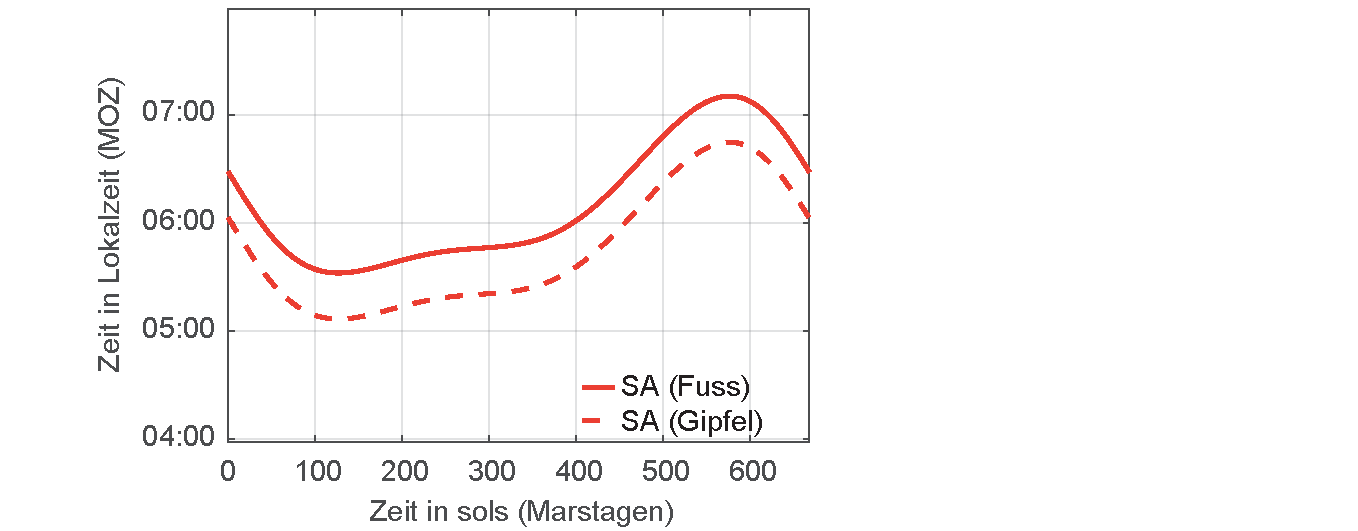
\includegraphics[width=\columnwidth]{OlympusMons.pdf}%
\caption[Sonnenaufgangszeiten auf dem Mars.]{Sonnenaufgangszeiten auf dem Mars am Fu� und auf dem Gipfel des Olympus Mons im Verlauf eines Mars-Jahres. Das Mars-Sommer Halbjahr erstreckt etwa von Tag 1 bis Tag 450 und damit wesentlich l�nger als das Winterhalbjahr.}%
\label{abb:hm_Mars_Sunrise_lsg}%
\end{figure}
\medskip \end{sol}
\textcolor{blue} {$\rightarrow$ zur} \probref{hm_sonnenaufgang_mars}.\\
\noindent\rule[1ex]{\textwidth}{0.5pt} \newpage

%-----------------------------------------------------------------------------------------------------------
\newpage
%%%-----------------------------------------------------------------------------------------------------------
\subsection{�bungen zu Monden, Kometen und Asteroiden}

\medskip

\begin{sol}{prob:hm_MondbahnHelioz}\label{lsg:hm_MondbahnHelioz} %�bung24
\textbf{Heliozentrische Mondbahn} \\

Heliozentrisch betrachtet l�uft der Mond um die Sonne und wird dabei von der Erde ein wenig abgelenkt. Die Mondbahn ist aber stets
zur Sonne hin gekr�mmt, und die St�rke dieser Kr�mmung �ndert
sich im Lauf eines Monats nur m��ig, da die Gravitationskraft
der Sonne am Ort des Mondes zu jeder Zeit deutlich
gr��er als diejenige der Erde ist, was man leicht nachrechnen kann. 
Geozentrisch ist es aber ebenfalls richtig zu sagen,
dass der Mond um die Erde l�uft und dabei von der Sonne
gest�rt wird, was zu seiner komplexen Bahn f�hrt.
Es gilt aber auch hier, dass die Schwerkraft
der Erde am Ort des Mondes zu jedem Zeitpunkt deutlich gr��er ist als
die Gezeitenkraft der Sonne auf das Erde-Mond-System ist, denn sonst w�rde dieses ja auseinander gerissen werden (siehe \kap{hm_gezeiten}). Man kann auch sagen, dass nur die Differenz der solaren Einfl�sse auf Erde und Mond sich als St�rung der
geozentrischen Mondbahn auswirkt.\\
Man kann sich nun recht einfach �berlegen, unter welchen Bedingungen schleifen- oder wellenf�rmige Mondbahnen zustande kommen k�nnen.
Wir wollen vereinfachend annehmen, dass die Planetenbahn und zugeh�rige Mondbahn ann�hernd koplanar und zirkular sind, also
gegeneinander nur wenig geneigt und wenig exzentrisch sind. 
Aus der Gravitationsbeschleunigung und dem dritten Keplerschen Gesetz findet man
folgende Beziehungen:
\begin{itemize}
\item Fall 1: Konvexe Bahn (wie Erdmond) : $T_\text{M}^2/T_\text{P}^2 > a_\text{M}/a_\text{P}$
\item Fall 2: Schleifenbahn : $T_\text{M}/T_\text{P} < a_\text{M}/a_\text{P}$
\item Fall 3: Wellenbahn : $T_\text{M}/T_\text{P} > a_\text{M}/a_\text{P} > T_\text{M}^2/T_\text{P}^2$
\end{itemize}
Hierin sind $T_\text{M},\, T_\text{P}$ die Umlaufzeiten von Mond und Planet und $a_\text{M},\, a_\text{P}$ die entsprechenden Radien der Bahnen.
Die erste Bedingung besagt, dass die
Gravitationsbeschleunigung des Mondes
durch den Planeten kleiner ist als diejenige
durch die Sonne, was beim Erdmond sicher erf�llt ist. Die zweite Bedingung
besagt, dass die Umlaufgeschwindigkeit
des Mondes um den Planeten gr��er
ist als die Geschwindigkeit des Planeten
um die Sonne. Dies ist beim Erde Mond System nicht erf�llt. Wegen $a_\text{M} \ll a_\text{P}$ ergibt sich deshalb beim Mond der Erde nur eine geringf�gig ausgepr�gte Wellenbahn 
(\figref{hm_mondbahn_lsg02}).\\
Wir wollen das in einer einfachen, komplanaren Modellrechnung zeigen und schreiben: 
\begin{align}
\begin{split}
    x_\text{M} &= a_\text{P}\,\cos\Omega_\text{P} \,t + a_\text{M}\,\cos\omega_\text{M}\,t \\
    y_\text{M} &= a_\text{P}\,\sin\Omega_\text{P} \,t + a_\text{M}\,\sin\omega_\text{M}\,t
\end{split} \label{eq:hm_lsgmondb01}
\end{align}
$t=0$ wurde hier so gew�hlt, dass $\vec{r}\lk 0\rk = \vec{r}_\text{M,0}  =  \lk x_\text{M},y_\text{M} \rk= \lk a_\text{P} + a_\text{M},0\rk $ ist. \\
Unser Kurvenparameter ist die Zeit $t$. Wir wollen den Kr�mmungsradius $\varrho$ und die Konvexit�t $\eta = \D^2 y/\D x^2$ als Funktion der Zeit berechnen. Gilt $\eta > 0$ ist die Bahn konvex, f�r Zeitbereiche in denen $\eta <0$ ist die Bahn konkav. \\
In Parameterdarstellung ist der Kr�mmungsradius $\varrho$ gegeben durch:
\begin{align}
    \varrho = \Bigg|\frac{\lk \dot{x}^2+ \dot{y}^2\rk^\frac{3}{2}}{\lk \dot{x}\ddot{y} -\ddot{x}\dot{y}\rk}\Bigg| = \Bigg|\frac{\lk \dot{x}^2+ \dot{y}^2\rk^\frac{3}{2}}{\det\lk \dot{\vec{r}},\ddot{\vec{r}}\rk}\Bigg| \label{eq:hm_lsgmondb02} \,. 
\end{align}
\begin{table}[h!]
    \centering
    \begin{tabular}{l|rcrcr}
         & $T_\text{M}{}^2/T_\text{P}{}^2$ & & $a_\text{M}/a_\text{P}$&&$T_\text{M}/T_\text{P}$\\
         \rule{0pt}{1pt}& & & & &  \\
         \hline
         \rule{0pt}{1pt}& & & & &  \\
         \rule{0pt}{6pt}Fall 1~~~ & $~0.25$ & $>$ & $0.1$ & & $0.5$ \\
         \rule{0pt}{6pt}Fall 2~~~ & $~0.0025$ & & $0.1$ & $>$& $0.05$ \\
         \rule{0pt}{6pt}Fall 3~~~ & $~0.01$ & $<$ & $0.1$ & $\leq$& $0.1$ 
    \end{tabular}
\end{table}\\
Man erkennt deutlich, dass je nach Fall die Schleifenbahn, eine Art Epizykloide auf einem Kreis mit dem Radius $a_\text{P}-a_\text{M}$ oder eben eine sehr flache Welle darstellt. Das Erde-Mond System f�llt in die Kategorie des Fall 1 mit $a_\text{P} \gg a_\text{M}$.\\
F�r stark geneigte Bahnen ergben sich durch notwendige Ber�cksichtigung der Bahnneigung etwas durch die Inklination
$\cos i$ modifizierte Beziehungen.\\
Die numerische Berechnung der 3 Beispiele ist mit entsprechenden Modellparametern sehr einfach zu realisieren und im \mscr{} \mlhmref{Mondbahn01.m} f�r koplanare kreisf�rmige Bahnen ausgef�hrt. Im \mscr{} \mlhmref{Mondbahn02.m} ist auch die heliozentrische Mondbahn aus den genauen Ephemeriden berechnet (\figref{hm_mondbahn_lsg03}).

\begin{figure}[H]
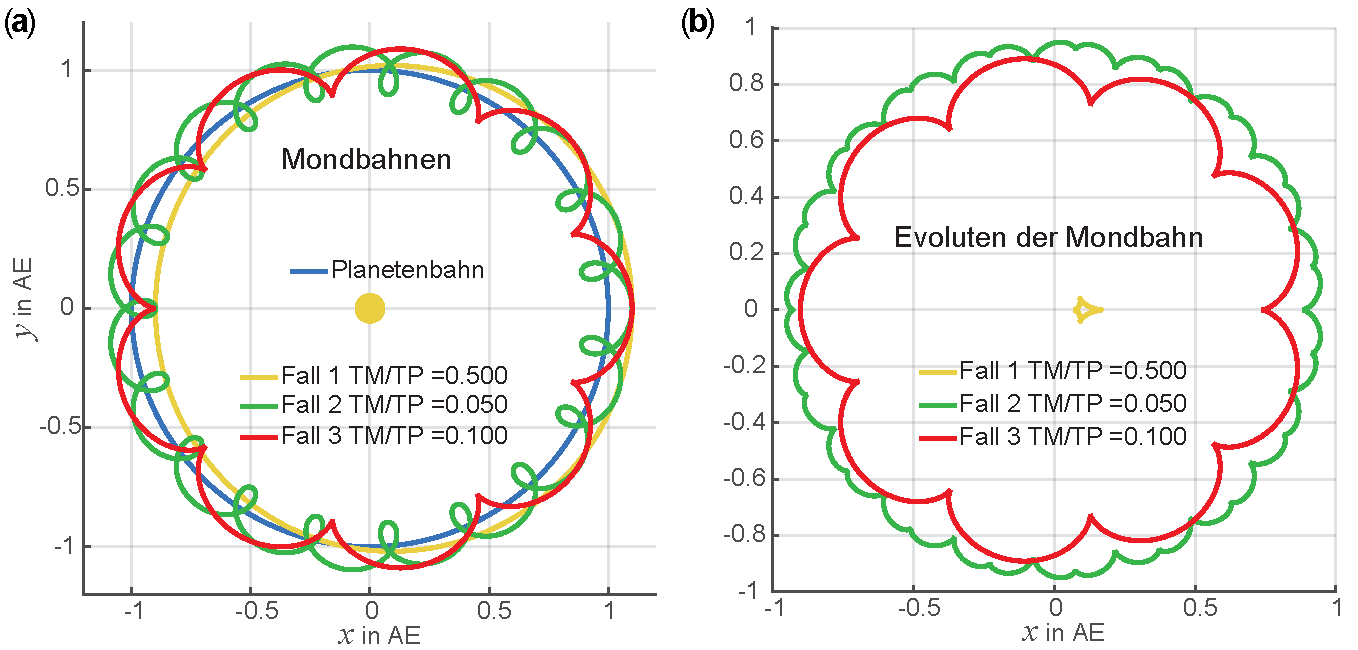
\includegraphics[width=\textwidth]{MondbahnHelioz3.pdf}
\caption[Heliozentrische Mondbahnen f�r koplanare, kreisf�rmige Bahnen.]{Heliozentrische Mondbahnen f�r koplanare, kreisf�rmige Bahnen Planet und Mond. \fa Mondbahnen \fb Lage der Mittelpunkte des lokalen Kr�mmungskreises (Evolute der Mondbahn). Das Verh�ltnis der Bahnradien von Mondbahn zu Planetenbahn wurde fest zu 0.1 angenommen, variiert wurden die Umlaufzeiten \bzw nach dem 3. Keplerschen Gesetz die Massen von Zentralk�rper und Planet.}\label{abb:hm_mondbahn_lsg01}
\end{figure}

\begin{figure}[H]
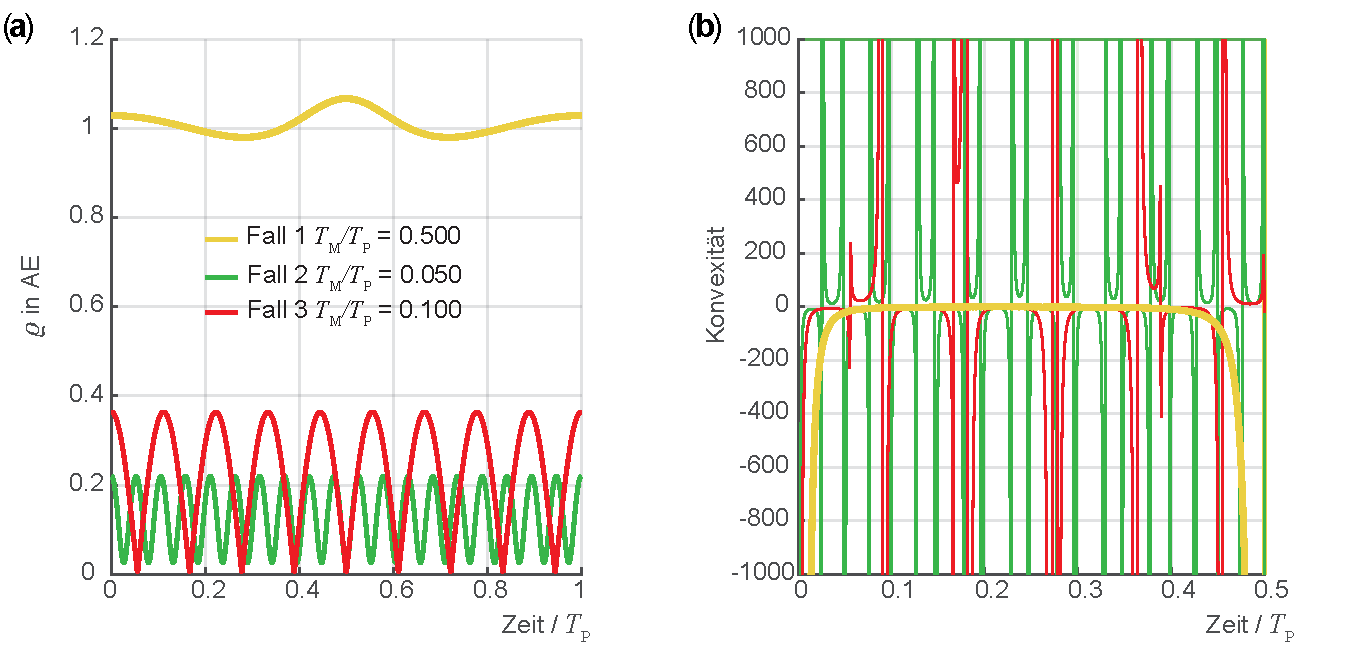
\includegraphics[width=\textwidth]{MondbahnHelioz4.pdf}
\caption[Kr�mmungsradius und Konvexit�t heliozentrischer Mondbahnen.]{Heliozentrische Mondbahnen f�r koplanare, kreisf�rmige Bahnen Planet und Mond. \fa Kr�mmungsradius \fb Konvexit�t. Das Verh�ltnis der Bahnradien von Mondbahn zu Planetenbahn wurde fest zu 0.1 angenommen, variiert wurden die Umlaufzeiten \bzw nach dem 3. Keplerschen Gesetz die Massen von Zentralk�rper und Planet.}\label{abb:hm_mondbahn_lsg02}
\end{figure}

\begin{figure}[H]
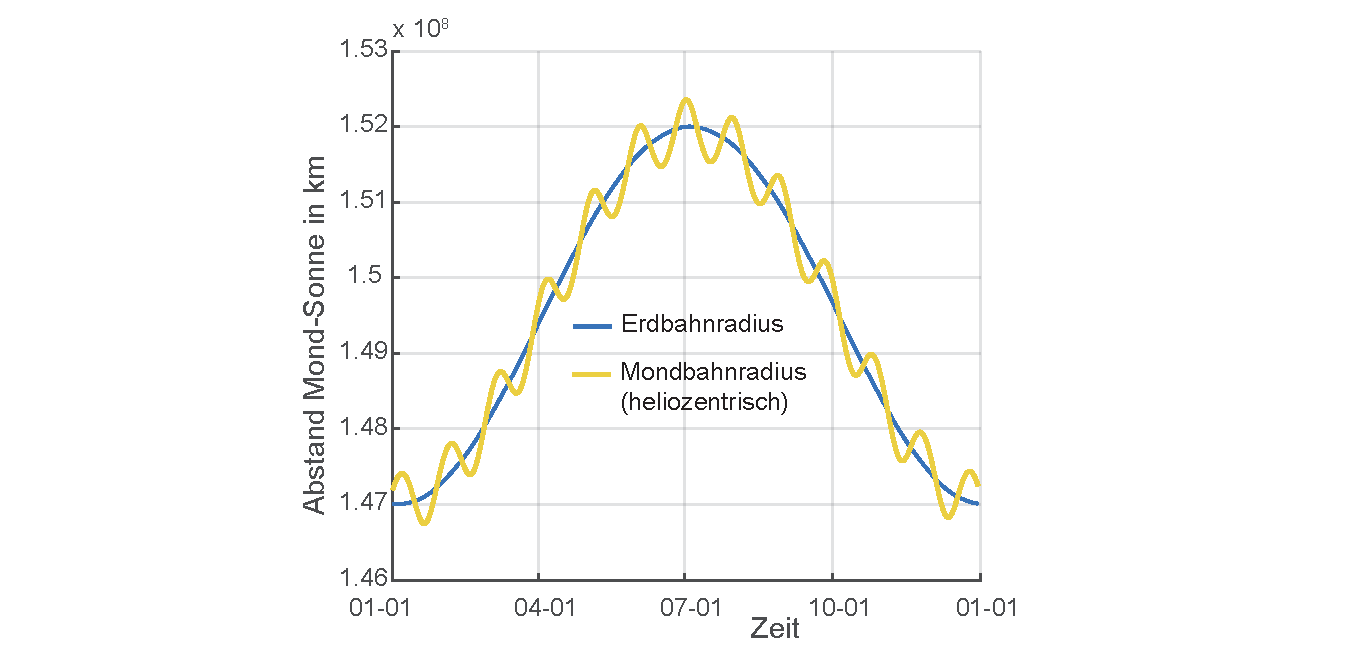
\includegraphics[width=\textwidth]{MondbahnHelioz2.pdf}
\caption{Heliozentrische Mondbahn aus den Ephemeriden berechnet}\label{abb:hm_mondbahn_lsg03}
\end{figure}


\medskip \end{sol}
\textcolor{blue} {$\rightarrow$ zur} \probref{hm_MondbahnHelioz}.\\
\noindent\rule[1ex]{\textwidth}{0.5pt} \newpage



%-----------------------------------------------------------------------------------------------------------

\begin{sol}{prob:hm_kometen_asteroiden} \label{lsg:hm_kometen_asteroiden} %�bung25
\textbf{Kometen und Asteroiden} \\ \\
Die Rechnungen sind im Detail in den einzelnen \mscren zu den Kometen- und Asteroidenbahnen \ua \mlhmref{AsteroidenBahnen.m} und \mlhmref{AsteroidenZeit.m} ausgef�hrt. Eine Beispielrechnung ist als Bild angef�gt. \\

\begin{figure}[H]
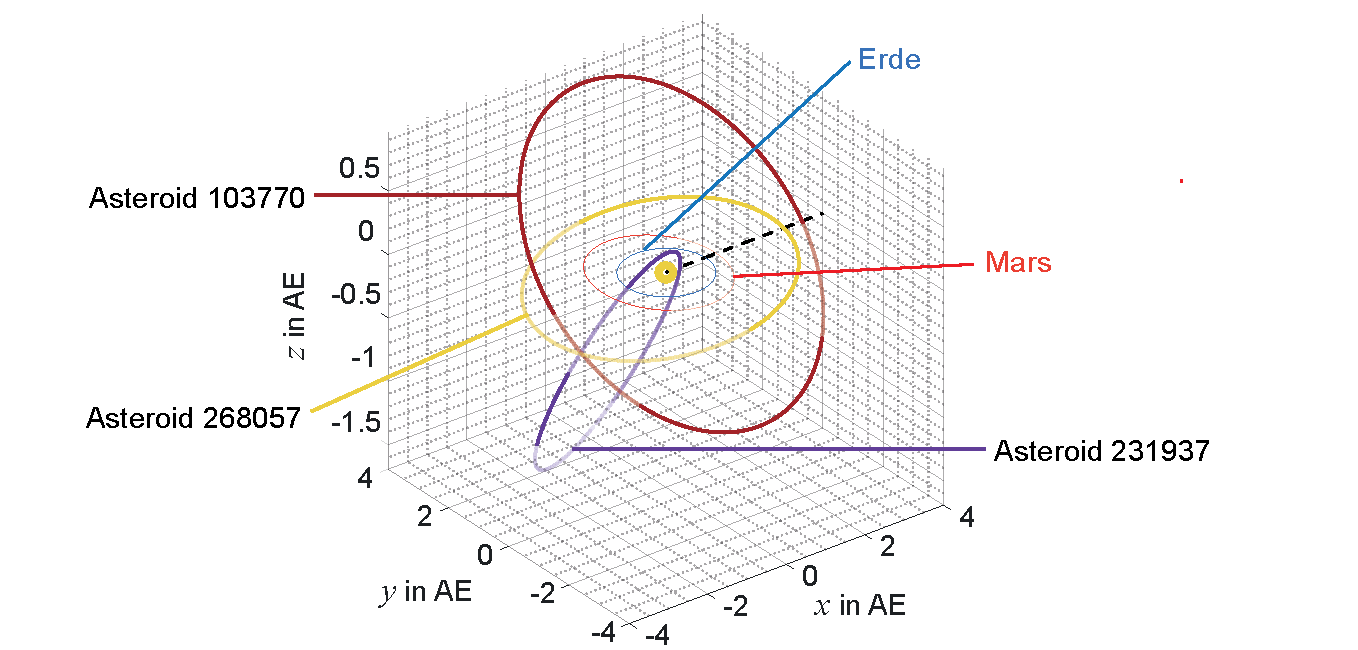
\includegraphics[width=\textwidth]{AsteroidenbahnenBeispiele.pdf}
\caption{Beispiele vo Asteroidenbahnen}\label{abb:hm_AsteroidenbahnenBeispiele}
\end{figure}

\medskip \end{sol}
\textcolor{blue} {$\rightarrow$ zur} \probref{hm_kometen_asteroiden}.\\
\noindent\rule[1ex]{\textwidth}{0.5pt} \newpage


%-----------------------------------------------------------------------------------------------------------


\begin{sol}{prob:hm_verweildauer_komet_erdbahn}\label{lsg:hm_verweildauer_komet_erdbahn} %�bung26
\textbf{Kometen und Meteoriten} \\
\begin{enumerate}[(a)]
	\item Wir vereinfachen zun�chst das Problem und nehmen an, dass die Kometenbahn in der Ekliptik liegt und dass diese in der N�he ihres Perihels als Parabel beschrieben werden kann.
          Somit ist die Exzentrizit�t $e\!=\!1$ und \eqref{eq:hm_kegelschnitt} vereinfacht sich zu
\begin{equation}
r = \frac{p}{1+\cos\upsilon}~~\text{mit}~~p=\frac{L^2}{\mu_\text{G}} ~~.\label{eq:hm_hmlsg_24_1}
\end{equation}
Der minimale Abstand ist demnach $r_\text{min}\!=\!q\!=\!p/2\!=\!L^2/(2\mu_\text{G})$.
F�r die spezifische Energie des Kometen gilt nach \eqref{eq:hm_total_energy} im Fall von Parabeln
\begin{equation}
H = \frac{1}{2}\dot{r}^2 + \frac{L^2}{2r^2} + U(r) ~~. \label{eq:hm_hmlsg_24_2}
\end{equation}
Am Perihel mit Abstand $r_\text{min} = q$ ist die Radialgeschwindigkeit $\dot{r}\!=\!0$, so dass
\begin{align*}
	\frac{L^2}{2r_\text{min}^2} &= -U(r_\text{min}) = \frac{\mu_\text{G}}{r_\text{min}} = \frac{\mu_\text{G}}{q} \\
	\Rightarrow L &= \sqrt{2\mu_\text{G}\,q}~~.
\end{align*}
Wir dr�cken nun den Perihelabstand als $q\!=\!r_\text{min}\!=\!ka_\text{\earth}\!=\! k\, 1\text{AE}$ mit $0\!<\!k\!<\!1$ aus.
Mit $\D t\!=\!\D r/\dot{r}$ und $\dot{r}\!=\!\sqrt{2[-U(r)-L^2/(2r^2)]}$ folgt aus \eqref{eq:hm_hmlsg_24_2}
\begin{align*}
	t-t_0 &= \int\limits_{q}^{r=a_\text{\earth}} \frac{r}{\sqrt{2\mu_\text{G}r-L^2}}\,\D r = \sqrt{\frac{1}{2\mu_\text{G}}} \int\limits_{q}^{r} \frac{r}{\sqrt{r-L^2/2\mu_\text{G}}}\,\D r ~~.\\
\end{align*}
In Integraltafeln finden wir als L�sung f�r das Integral
\begin{equation*}
t-t_0 = \frac{1}{\sqrt{2\mu_\text{G}}}\,\frac{2}{3}\,\sqrt{r-q}\,(2q+r) \bigg|^{a_\text{\earth}}_{q}~~.
\end{equation*}
Die Gesamtaufenthaltsdauer des Kometen innerhalb der Erdbahn, in welcher der Komet gut beobachtet werden kann, ist dann gegeben durch
\begin{align}
	T_\text{ges} &= \frac{2}{\sqrt{2\mu_\text{G}}}\,\frac{2}{3}\,\lek \sqrt{a_\text{\earth}-ka_\text{\earth}} \lk 2ka_\text{\earth} + a_\text{\earth} \rk - \sqrt{q-q} \lk 2ka_\text{\earth} + a_\text{\earth} \rk \rek \\
	 &= \frac{2}{\sqrt{2\mu_\text{G}}}\,\frac{2}{3}\,\sqrt{a_\text{\earth}^3}\,\sqrt{1-k}\,(2k+1) = \frac{4}{3}\,\sqrt{\frac{a_\text{\earth}^3}{2\mu_\text{G}}}\,\sqrt{1+3k-4k^3}~~. \label{eq:hm_verweildauer01}
\end{align}
\begin{figure}[H]
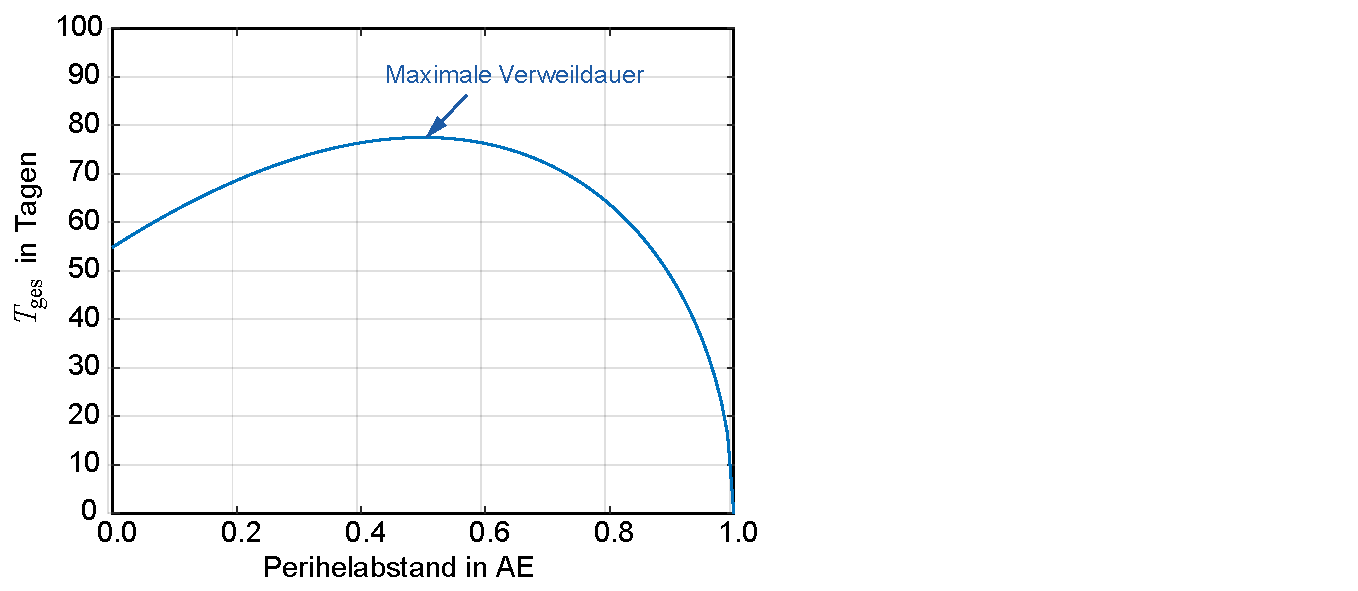
\includegraphics[width=\textwidth]{Verweildauer.pdf}%
\caption[Verweildauer des Kometen in Tagen innerhalb der Erdumlaufbahn.]{Verweildauer des Kometen in Tagen innerhalb der Erdumlaufbahn (Kriterium f�r gute Sichtbarkeit).}%
\label{abb:hm_aufenthaltsdauer_lsg}%
\end{figure}
Die \figref{hm_aufenthaltsdauer_lsg} zeigt die Verweildauer normiert auf die Umlaufdauer der Erde gem��
\begin{equation}
\frac{T_\text{ges}}{2\pi\sqrt{a_\text{\earth}^3/\mu_\text{G}}} = \frac{2}{3}\frac{1}{\sqrt{2}\pi}\,\sqrt{1+3k-4k^3}~~.\label{eq:hm_verweildauer02}
\end{equation}
Man erkennt, dass je kleiner der Perihelabstand ist, desto h�her wird die Geschwindigkeit des Kometen und desto k�rzer seine Aufenthaltsdauer innerhalb der Erdbahn, desto heller leuchtet er aber auch.
Interessant ist auch, dass die maximale Dauer auf etwa 80 Tage begrenzt ist.\\

\item Wir betrachten einen Meteoroiden, der sich im Schwerefeld von Sonne und Erde bewegt (\figref{hm_aufschlaggeschw}):
Wir wollen seine Position zun�chst in einem rotierenden KOS betrachten, das sich mit der Winkelgeschwindigkeit $\omega$ der Erde um Sonne mitdreht (\vgl dazu auch die Darstellungen in  Kap 1.2.3.6  in Band I).
Die spezifische Energie des Himmelsk�rpers im Abstand $r_\text{K}$ mit der Geschwindigkeit $v_\text{K}$ ist dann gegeben durch (wir lassen die Striche f�r das mitbewegte \KOS{} weg, der Index K steht f�r den Kometen im mitbewegten System):
\begin{equation}
 H_\text{K} = \frac{v_\text{K}^2}{2} - \frac{\mu_\text{G}m_\text{\earth}}{r_\text{K} m_\text{\astrosun}} - \frac{\mu_\text{G}}{r_\text{SK}} - \frac{\omega^2}{2}\,(x_\text{K}{}^2 + y_\text{K}{}^2)~~,
\label{eq:hm_hmlsg_24b_1}
\end{equation}
worin $\omega\!=\!\sqrt{\mu_\text{G}/a_\text{\earth}^3}$ gem�� \eqref{eq:hm_1-ecosEdE} ist, der zweite und dritte Term die potentielle Energie bzgl. der Erde und der Sonne repr�sentieren und der letzte Term das Zentrifugalpotential, hervorgerufen durch das rotierende KOS, darstellt.
Wir setzen $\alpha\!=\!m_\text{\earth}/m_\text{\astrosun}$. 

\begin{figure}[H]
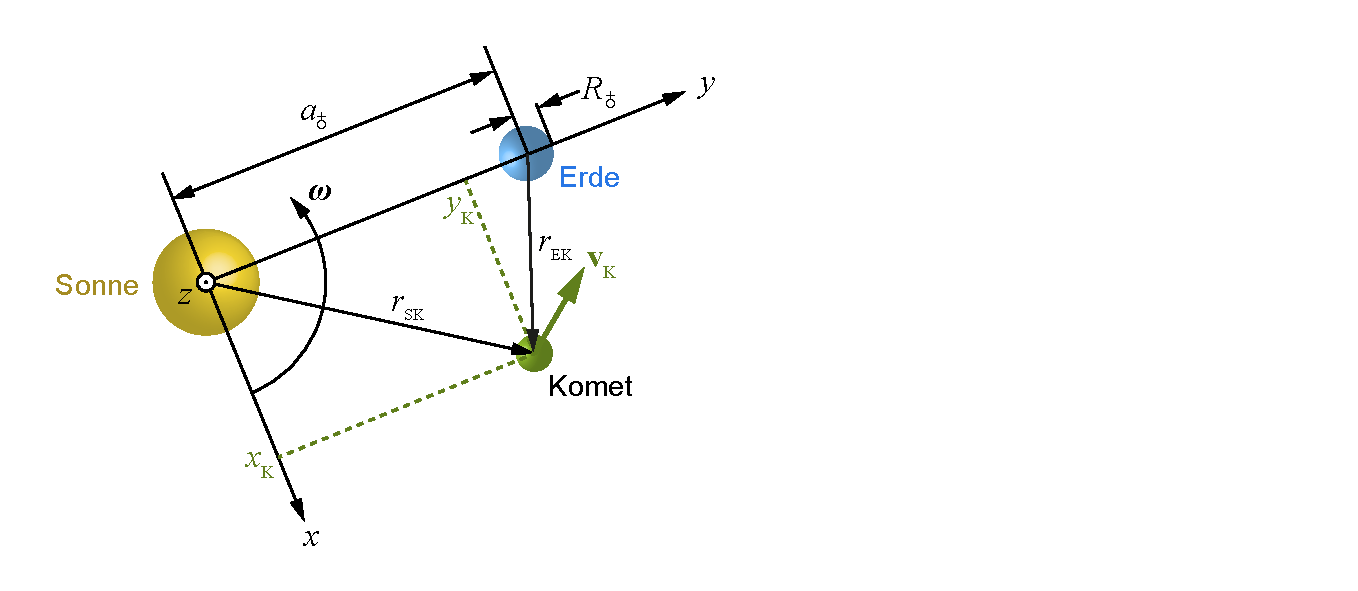
\includegraphics[width=\textwidth]{AufprallKomet.pdf}%
\caption{Zur Berechnung der Aufschlaggeschwindigkeit eines Kometen}%
\label{abb:hm_aufschlaggeschw}%
\end{figure}

F�r den Moment des Aufschlags gilt:
\begin{align}
H_\text{K,A} (r_\text{K}=R_\text{\earth}) &= \frac{v_\text{A}^2}{2} - \frac{\alpha \mu_\text{G}}{R_\text{\earth}} - \frac{\mu_\text{G}}{a_\text{\earth}} - \frac{\omega^2}{2}\,a_\text{\earth}^2 
= \frac{v_\text{A}^2}{2} - \frac{\alpha \mu_\text{G}}{R_\text{\earth}} - \frac{3\mu_\text{G}}{2a_\text{\earth}} ~~. \label{eq:hm_hmlsg_24b_2} 
\end{align}
F�r eine initiale Position mit $r_0\!\gg\! a_\text{\earth}$ k�nnen wir wegen $\alpha\!\gg\! 1$ in \eqref{eq:hm_hmlsg_24b_1} den zweiten Term vernachl�ssigen und erhalten
\begin{equation}
H_{\text{K},0} = \frac{v_0{}^{2}}{2} - \frac{\mu_\text{G}}{r_0} - \frac{\omega^2}{2}\,(x_0{}^{2} + y_0{}^{2}) ~~. 
\end{equation}
Jetzt verlassen wir das rotierende KOS und gehen in das in der Sonne verankerte Inertialsystem �ber. \label{eq:hm_hmlsg_24b_2a} 
Dann gilt f�r die Geschwindigkeit des Himmelsk�rpers in diesem KOS (man beachte die Richtung von $\vec{\omega}$):
\begin{equation}
\vec{v}_0 = \vec{v}_\text{S} - \vec{\omega}\times\vec{r}_\text{S} ~~,\label{eq:hm_hmlsg_24b_3}
\end{equation}
wobei die Indizes S die Gr��en im Inertialsystem der Sonne kennzeichnen. 
Wir k�nnen dann schreiben:
\begin{equation}
v_0{}^2 = v_\text{S}{}^{2} - 2\,\vec{v}_\text{S}(\vec{\omega}\times\vec{r}_\text{S}) + \omega^2({x_\text{S}}^2 + {y_\text{S}}^2) ~~.
\label{eq:hm_hmlsg_24b_4}
\end{equation}
Wir setzen \eqref{eq:hm_hmlsg_24b_4} in \eqref{eq:hm_hmlsg_24b_3} ein und ber�cksichtigen, dass gilt:
\begin{align*}
\vec{r}_0{}^2 &= {x_0}^{2} + {y_0}^{2} = {x_\text{S}}^{2} + {y_\text{S}}^{2} = {\vec{r}_\text{S}}^2 ~~~\text{und} ~~~ \vec{v}_\text{S}(\vec{\omega}\times\vec{r}_\text{S}) = \vec{\omega}(\vec{r}_\text{S}\times\vec{v}_\text{S}) = \vec{\omega}\,\vec{L} \,.
\end{align*}
Hierin ist $\vec{L}$ der konstante Drehimpuls des Kometen im Inertialsystem der Sonne ist.
Somit erhalten wir f�r die Energie
\begin{equation}
H_\text{K,S} = \frac{v_\text{S}^2}{2} - \frac{\mu_\text{G}}{r_\text{S}} - \omega L\cos i_\text{K}~~,
\label{eq:hm_hmlsg_24b_5}
\end{equation}
worin der Winkel $i_\text{K}$ die Neigung der Bahn des Himmelsk�rpers gegen die Ekliptik ist.
Setzen wir wegen der Energieerhaltung $H_\text{K,0}\!=\!H_\text{K,S}\!=\!H_\text{K,A}$, so erhalten wir f�r die Geschwindigkeit $v_\text{A}$ beim Aufschlag:
\begin{equation}
v_\text{A}{}^2 = \frac{2 \alpha \mu_\text{G}}{R_\text{\earth}} + \frac{3\mu_\text{G}}{a_\text{\earth}} + C_\text{J} - 2,\omega L\cos i_\text{K} ~~.
\label{eq:hm_hmlsg_24b_6}
\end{equation}
Darin haben wir die sogenannte Jacobi-Konstante\index{Jacobi-Konstante} $C_\text{J}\!=\!v_0^2 - 2\,\mu_\text{G}/r_0$ eingef�hrt, welche der doppelten spezifischen Energie des Himmelsk�rpers entspricht, wenn dieser nur dem Schwerefeld der Sonne ausgesetzt w�re. Sie dazu auch die Definition $C_\text{J}$ im Kap 1.2.3.6 in Band I.
Wir k�nnen nun mit den Beziehungen \eqref{eq:hm_drehimpuls_von_ae} f�r den Drehimpuls bzw. dem vis-viva-Satz \eqref{eq:hm_vis-viva} die Gr��en $L$ und $H_\text{J}$ durch die geometrischen Bahnparameter $a_\text{K}$ und $e_\text{K}$ ersetzen.
Wir erhalten nach einigen algebraischen Umformungen
\begin{equation}
v_\text{A} = \sqrt{\frac{2\alpha\mu_\text{G}}{R_\text{\earth}} + \underbrace{\frac{\mu_\text{G}}{a_\text{\earth}} \lek 3-\lk \frac{a_\text{\earth}}{a_\text{K}} + 2\cos i_\text{K}\,\sqrt{\frac{a_\text{K}}{a_\text{\earth}}\,(1-e_\text{K}^2)} \rk \rek }_{U^2}} ~~.
\label{eq:hm_hmlsg_24b_7}
\end{equation}
Das ist schon unsere L�sung.
Der erste Term unter der Wurzel ist eine Konstante und nichts anderes als das Quadrat der 2. kosmischen Geschwindigkeit \index{Kosmische Geschwindigkeit}
\begin{equation*}
v_\text{kos,II} = \sqrt{\frac{2\alpha\mu_\text{G}}{R_\text{\earth}}} = \sqrt{\frac{2Gm_\text{\earth}}{R_\text{\earth}}} = 11.2\:\text{km/s}~~.
\end{equation*}
Im zweiten Term unter der Wurzel identifizieren wir einerseits die 3. kosmische Geschwindigkeit
\begin{equation*}
v_\text{kos,III} = \sqrt{\frac{\mu_\text{G}}{a_\text{\earth}}} = 29.7\:\text{km/s}
\end{equation*}
und definieren andererseits den Term in der eckigen Klammer als Funktion $f(a_\text{K},e_\text{K},i_\text{K})$.
Dadurch l�sst sich \eqref{eq:hm_hmlsg_24b_7} deutlich vereinfacht schreiben als
\begin{equation}
v_\text{A} = \sqrt{v_\text{kos,II}^2 + v_\text{kos,III}^2 \, f(a_\text{K},e_\text{K},i_\text{K})} =\sqrt{v_\text{kos,II}^2  + U^2}~~.
\label{eq:hm_hmlsg_24b_8}
\end{equation}
Wir k�nnen die Aufschlaggeschwindigkeit \eqref{eq:hm_hmlsg_24b_8} auch schreiben als
\begin{equation}
v_\text{A} = v_\text{kos,III}\,\sqrt{p_\text{\earth} - \lk \frac{a_\text{\earth}(1-e)}{a_\text{K}} + 2\cos i_\text{K} \sqrt{\frac{(1+e_\text{K})a_\text{K}}{a_\text{\earth}}}\rk}
\label{eq:hm_hmlsg_24b_9}
\end{equation}
mit $p_\text{\earth}\!=\!\lk 3 + 2\alpha a_\text{\earth}/R_\text{\earth} \rk \!\approx\! 3.1411$.
F�r langgestreckte Ellipsen $e\!\rightarrow\! 1$ ist die Periheldistanz $q_\text{K}/(1-e)\!\gg\! a_\text{\earth}$ und $1+e_\text{K}\!\approx\! 2$, so dass \eqref{eq:hm_hmlsg_24b_9} geschrieben werden kann als 
\begin{equation}
v_\text{A} = v_\text{kos,III}\,\sqrt{p_\text{\earth}-2\cos i_\text{K}\sqrt{\frac{2q_\text{K}}{a_\text{\earth}}}} ~~,
\label{eq:hm_hmlsg_24b_10}
\end{equation}
was in der \figref{hm_aufschlaggeschw_2} f�r verschiedene Periheldistanzen und Bahnneigungen dargestellt ist.
Wenn man annimmt, dass der Komet/Meteor bei seiner Periheldistanz die Erde trifft, dann gilt $q_\text{K}=a_\text{\earth}$ und wir k�nnen aus der Abbildung die minimale Aufprallgeschwindigkeit von 16.6 km/s bei $i_\text{K} = 0\degree$ und die maximale von 72.6 km/s bei $i_\text{K} = 180\degree$ ablesen.
\begin{figure}[H]
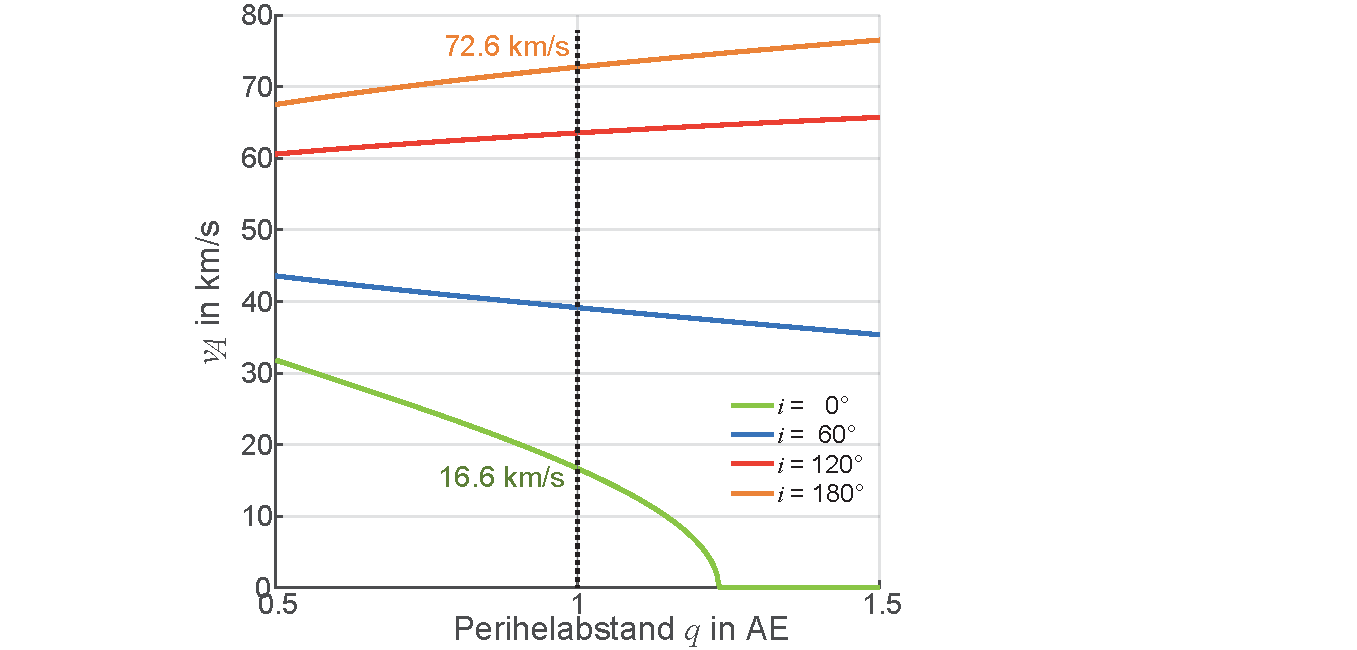
\includegraphics[width=\textwidth]{Aufschlaggeschwindigkeit.pdf}%
\caption[Aufschlaggeschwindigkeit eines Kometen.]{Berechnete Aufschlaggeschwindigkeit eines Kometen f�r verschiedene Bahnneigungen als Funktion des Perihelabstandes.}%
\label{abb:hm_aufschlaggeschw_2}%
\end{figure}

Wir k�nnen \eqref{eq:hm_hmlsg_24b_7} und \eqref{eq:hm_hmlsg_24b_9} auch benutzen, um die im Beispiel \ref{bsp:hm_shoemaker_levy} berechnete Aufschlaggeschwindigkeit des Kometen SL9 zu �berpr�fen.
Wir m�ssen in unseren Gleichungen nur folgende Ersetzungen vornehmen:
\begin{align*}
	a_\text{\earth} &\rightarrow a_\text{\jupiter} = 5.204\:\text{AE} \\
	R_\text{\earth} &\rightarrow R_\text{\jupiter} = 71492\:\text{km} \\
	\alpha &\rightarrow \alpha_\text{\jupiter} = \frac{m_\text{\jupiter}}{m_\text{\astrosun}} = 0.955\cdot 10^{-3} ~~.
\end{align*}
Mit diesen Werten und den Bahnparametern von SL9 aus Tabelle \ref{tab:hm_bahnparameter} erhalten wir $v_\text{A,SL}\!=\!59.5\:\text{km/s}$, was gut mit den numerisch berechneten Werten in Beispiel \ref{bsp:hm_shoemaker_levy} �bereinstimmt.\\

\item Aus \eqref{eq:hm_Shoemaker1979} erh�lt man f�r die kinetische Energien des Meteoriten im N�rdlinger Ries \bzw Steinheimer Becken
\begin{equation*}
T_\text{N} \approx 141\:\text{Gt TNT}  ~~ \text{bzw.} ~~ T_\text{S} \approx 268\:\text{Mt TNT} ~~.
\end{equation*}
Zum Vergleich, die Atombombe von Hiroshima hatte eine Sprengkraft von \anf{nur} ca. $12\:\text{kt TNT}$.
Die Energien von solchen Asteroiden/Meteoriten sind also unglaublich hoch (Man dr�cke diese einmal in konventionellen Gr��en ($1\:$kt TNT entspricht $4.185\cdot 10^{12}\:\text{J}$ aus.).\\
Unter Annahme eines kugelf�rmigen Himmelsk�rpers mit der Dichte $\rho\!=\!2.8\:\text{g/cm}^3$ kann man den Durchmesser des Meteoriten absch�tzen.
Im L�sungsteil (b) (\figref{hm_aufschlaggeschw_2}) hatten wir f�r $v_\text{min}$ und $v_\text{max}$ Werte zwischen 16 und 70 km/s erhalten.
Da es sehr wahrscheinlich ist, dass die Inklination der Asteroidenbahn zwischen $20\degree$ und $45\degree$ lag, k�nnen wir von Aufschlaggeschwindigkeiten zwischen $20$ km/s und $30$ km/s ausgehen.
Es ergeben sich dann Asteroidendurchmesser im Fall des N�rdlinger Ries von
\begin{equation*}
D_\text{N} = 2\,\sqrt[3]{\frac{T_\text{N}}{\pi\rho v_\text{A}^2}} = 1.0\:\text{km}~\ldots~ 1.3\:\text{km}
\end{equation*}
und im Fall des Steinheimer Beckens von
\begin{equation*}
D_\text{S} = = 0.5\:\text{km}~\ldots~ 0.65\:\text{km}~.
\end{equation*}

\begin{figure}[H]
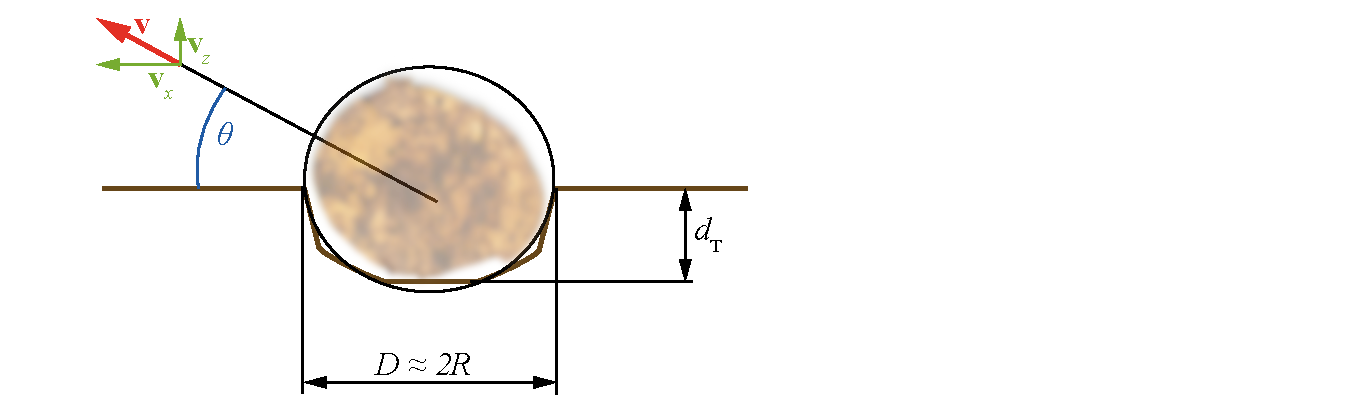
\includegraphics[width=\textwidth]{Meteorkrater.pdf}%
\caption{Zur Berechnung der Aufschlaggeschwindigkeit eines Kometen}%
\label{abb:hm_shoemaker_deriv}%
\end{figure}

Wir wollen jetzt noch eine Absch�tzung f�r die Shoemaker-Formel geben. Dazu nehmen wir an, dass die vom Asteroiden (oder einem anderen Himmelsk�rper) ausgeworfene Kratermasse unter einem Winkel von $\theta$ und mit einer Geschwindigkeit $v$ wegfliegt. Die Mindestzeit, die die ausgeworfene Masse in der Luft sein muss, ergibt sich nach \figref{hm_shoemaker_deriv}
zu:
	\[t = 2 v_z/g = 2v\sin\theta/g
\]
In dieser Zeit muss der Kraterdurchmesser $D=2 R$ "`ausgehoben"' werden, also:
	\[ D = v_x\,t = 2v^2\,\sin\theta \cos\theta/g = v^2 \,\sin(2\theta)/g \leq v^2/g\,
\]
woraus folgt : $v_\text{min} = \sqrt{D\,g}$.
Die Masse des Aushubs ist (Krater als zylinderf�rmig angenommen):
	\[ m_\text{A} = \varrho\frac{\pi}{4}\,D^2\,d_\text{T}\,,
	\]
	mit $\varrho \approx \SI{4e3}{\kg\per\metre\cubed}$.
Damit ist eine minimale kinetische Energie verbunden, die den Auswurf "`wegtransportiert"';
	\[ T_\text{min} = \frac{m_\text{A}}{2} \,v^2 = \frac{\pi}{8}\varrho\,g\,d_\text{T}\,D^3\,.
	\]
Ber�cksichtigt man noch, dass wegen der Umwandlung in thermische Energie nur wenige Prozent $\eta = 1\% \ldots 4\%$ in kinetische Energie umgewandelt werden, dann gilt die Beziehung:
\begin{align}
T_\text{min}  = \tilde{\kappa}\,	T_\text{K} = \tilde{\kappa} \frac{\pi}{8}\varrho\,g\,d_\text{T}\,d_\text{T}\,D^3\,. \,. \label{eq:hm_shoemaker_verified}
\end{align}
Wir bekommen also ann�hernd den empirischen Zusammenhang $D \propto T_\text{K}^{1/3}$, wobei wegen $\tilde{\kappa} = \tilde{\kappa}(d)=\tilde{\kappa}(d(D))$ eine zus�tzliche $D-$Abh�ngigkeit ergibt, die sich in der Shoemaker-Formel im Exponenten zeigt. Wir �berlassen es dem Leser, in Formel \eqref{eq:hm_shoemaker_verified} den Proportionalit�tsfaktor $\tilde{\kappa}$ auszurechnen und zu verifizieren, dass sich tats�chlich solche gigantischen Energien ergeben.\\

\item Nehmen wir an, dass der Planetoid (Meteor) mit Masse $m_\text{P}$ einen Mond der Masse $m_\text{M}$ hatte.
  Dann zieht der Planetoid den Mond mit der Kraft $F_\text{P}\!=\! Gm_\text{P}m_\text{M}/d^2$ an.
  Andererseits wirkt auf die beiden K�rper die Gravitationskraft der Sonne in unterschiedlichem Ma�e (Gezeitenkraft) (siehe \kap{hm_gezeiten}), die die beiden K�rper zu trennen versucht. F�r f�r die Gezeitenkraft gilt:
\begin{equation*}
F_\text{Gez} \approx \frac{2Gm_\text{M}m_\text{\astrosun}\,a_\text{PM}}{a_\text{\earth}^3}~~,
\end{equation*}  
worin $a_\text{PM}$ der Abstand zwischen Planetoid und Mond ist.
Das System des Doppelplanetoiden (bzw. Planetoid mit Mond) ist stabil, wenn $F_\text{P}\!>\!F_\text{Gez}$, also
\begin{equation*}
\frac{Gm_\text{P}m_\text{M}}{a_\text{PM}{}^2} > \frac{2Gm_\text{M}m_\text{\astrosun}\, a_\text{PM}}{a_\text{\earth}^3}~~.
\end{equation*}
Dies ist erf�llt, wenn
\begin{equation*}
	a_\text{PM} < \sqrt[3]{\frac{m_\text{P}}{2m_\text{\astrosun}} a_\text{\earth}^3} = a_\text{\earth}\,\sqrt[3]{\frac{m_\text{P}}{2m_\text{\astrosun}}} ~~.
\end{equation*}
Mit der Masse $m_\text{P}\!=\!\rho_\text{P}V_\text{P}$ aus Aufgabenteil (c) erhalten wir $a_\text{PM}\!\leq\! 150\:$km.
Verglichen mit dem Abstand der beiden Einschlagkrater von $40\:$km ist es also wahrscheinlich oder zumindest m�glich, dass der Doppelkrater vor 15 Millionen Jahren durch einen Doppelplanetoiden bzw. Planetoid und zugeh�riger Mond verursachte wurde.
\end{enumerate}
Die �bungsaufgabe und deren L�sung basiert auf der Darstellung �hnlicher Probleme in \cite{Garfinkle2014} und \cite{Quetz2017}.
Wir verweisen auch auf das entsprechende \mscr~\mlhmref{VerweildauerKomet.m} sowie \mlhmref{AufprallgeschwindigkeitKomet.m}.
\medskip \end{sol}

\textcolor{blue} {$\rightarrow$ zur} \probref{hm_verweildauer_komet_erdbahn}.\\
\noindent\rule[1ex]{\textwidth}{0.5pt} \newpage


%-----------------------------------------------------------------------------------------------------------

\begin{sol}{prob:hm_Doppelstern}\label{lsg:hm_Doppelstern} %�bung27
\textbf{Doppelstern-System - Vergleich numerische und analytische L�sung} \\ \\

Die Rechnungen finden sich f�r ein Modellsystem mit Massenverh�ltnis 2.5:1 und einem anf�nglichen Abstand von 2\,AE, sowie anf�nglichen Geschwindigkeiten in Oppositionsstellung von $v_0 = \SI{-5}{\km\per\second}$ \bzw $v_0 = \SI{20}{\km\per\second}$ in den \mscr en \mlhmref{Doppelsternsystem.m} (Inertialsystem) \bzw \mlhmref{DoppelsternsystemCOM.m} (Schwerpunktsystem). L�sungen sind beispielhaft in den folgenden Abbildungen gezeigt.\\
%Die numerische �bereinstimmung mit der analytischen L�sung ist ausgezeichnet.
\begin{figure}[H]
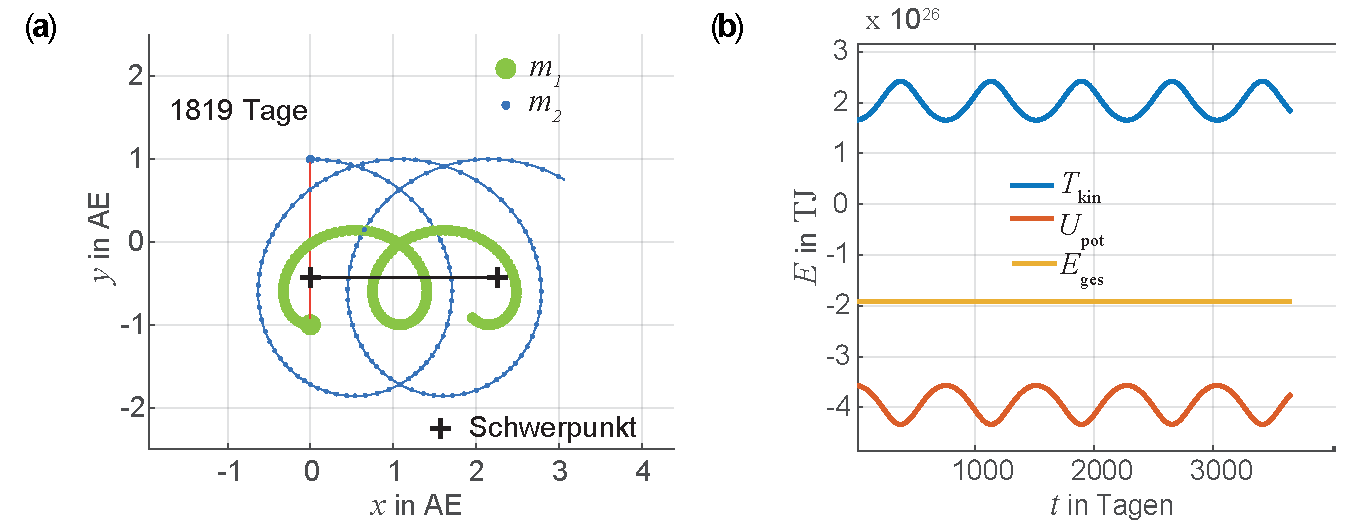
\includegraphics[width=\textwidth]{DoppelsternEnergie.pdf}%
\caption{Trajektorie \fa und Energieanteile \fb eines Doppelsternsystems im Inertialsystem. Die Energieerhaltung mit dem Hin-und Herpendeln zwischen kinetischer und potentieller Energie ist gut zu erkennen}%
\label{abb:hm_doppelsternenergie}%
\end{figure}
\begin{figure}[H]
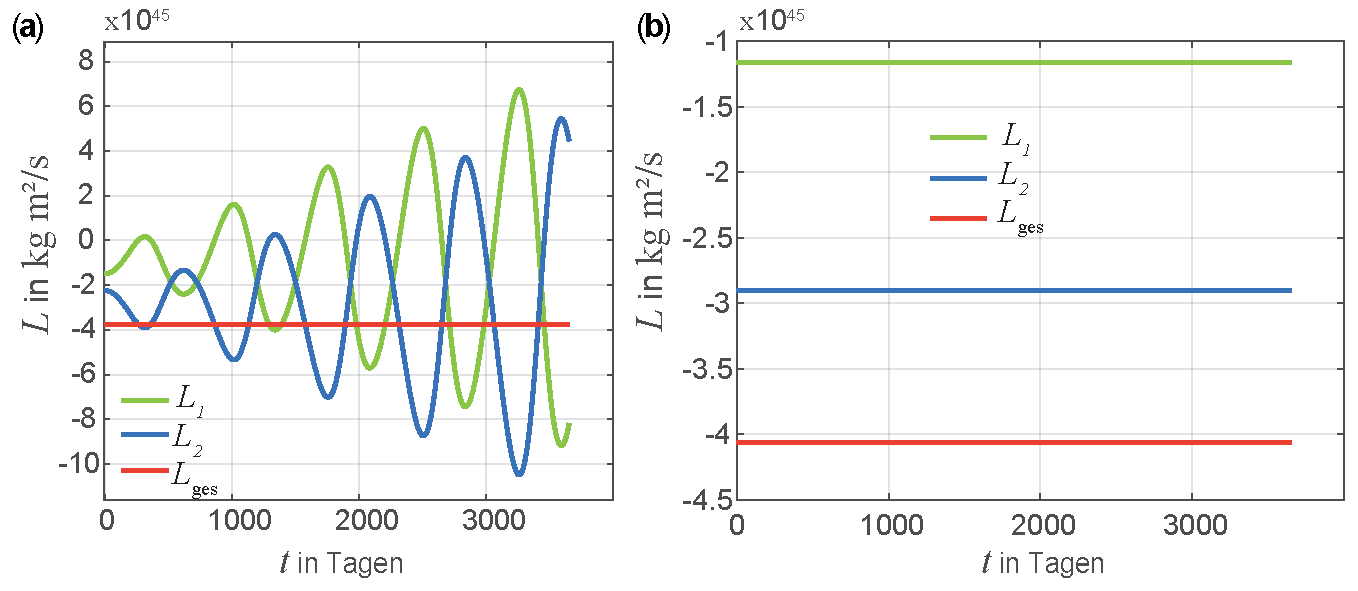
\includegraphics[width= \textwidth]{DoppelsternDrehimpulse.pdf}%
\caption{Drehimpulse eines Doppelsternsystems im Inertialsystem \fa und im Schwerpunktsystem \fb. Im Inertialsystem ist der Gesamtdrehimpuls erhalten}%
\label{abb:hm_doppelsterndrehimpulse}%
\end{figure}
\end{sol}
\textcolor{blue} {$\rightarrow$ zur} \probref{hm_Doppelstern}.\\
\noindent\rule[1ex]{\textwidth}{0.5pt} \newpage

%-----------------------------------------------------------------------------------------------------------

\begin{sol}{prob:hm_Sonnensystem}\label{lsg:hm_Sonnensystem} %�bung28
\textbf{Sonnensystem - Numerische, Kepler- und JPL-Berechnung} \\ \\

Wir verweisen auf die \mscr e \mlhmref{SonnensystemSimulationKepler.m}, \mlhmref{SonnensystemSimulationJPL.m} und \mlhmref{SonnensystemSimulationLangeZeiten.m}.\\
Als Referenzdaten verwenden wir die Vektordaten aus \url{https://ssd.jpl.nasa.gov/horizons/} (\cite{JPL2020}).

Die Bewegungsgleichungen f�r die Beschleunigungen der einzelnen ($i,j = 1 \ldots 8$) Planeten und die beiden betrachteten Kometen ($i,j = 9,10$) und die Sonne ($i,j = =N=11$) lauten dann:
	\begin{align}
		 \vec{a}_i = \ddot{\vec{r}}_i = -\sum_{j, j \neq i}^{N} (\vec{r}_i-\vec{r}_j) \frac{G\,m_i}{|\vec{r}_i-\vec{r}_j|^3}~~~~i=1 \ldots N~\,. \label{eq:hm_PlanetenDGLSystem01}
	\end{align}
Hierin sind $\vec{r}_i$ und $m_i$ die Positionsvektoren \bzw die Massen der einzelnen Planeten,  Kometen und der Sonne. Der Index $i,kj=N+1$ bezieht sich dabei auf die Sonne.
Die DGLs \eqref{eq:hm_PlanetenDGLSystem01} werden mit den entsprechenden Anfangsbedingungen f�r die Himmelsk�rper numerisch integriert. 

In \figref{hm_SonnensystemSimulation01} vergleichen wir die Abweichungen der L�sungen f�r \eqref{eq:hm_PlanetenDGLSystem01}, die wir aus der L�sung der Kepler-Gleichung \bzw der St�rungstheorie und zum anderen �ber numerische Integration von \eqref{eq:hm_PlanetenDGLSystem01} erhalten haben. Die Anfangswerte $\vec{r}_i(t_0)$ und $\dot{\vec{r}}_i(t_0)$  beschaffen wir uns aus dem JPL-Webservice \url{https://ssd.jpl.nasa.gov/horizons/}. Bei der Erdbahn erkennt eine periodische Abweichung (im Monatsrhythmus) unserer Rechnung von der JPL-Berechnung, die nat�rlich, davon herr�hrt, dass wir den Mond in unseren Rechnungen nicht ber�cksichtigt haben. Ansonsten ist die �bereinstimmung aber sehr gut und die Rechnung viel genauer als die einfache Kepler-L�sung, was man auch an der berechneten Marsbahn sehr gut sieht (bei der ja kein Mond der Gr��enordnung des Erdmondes zu ber�cksichtigen ist). Wir empfehlen dem interessierten Leser, die Rechnungen unter Ber�cksichtigung des Mondes zu wiederholen.

\begin{figure}[H]
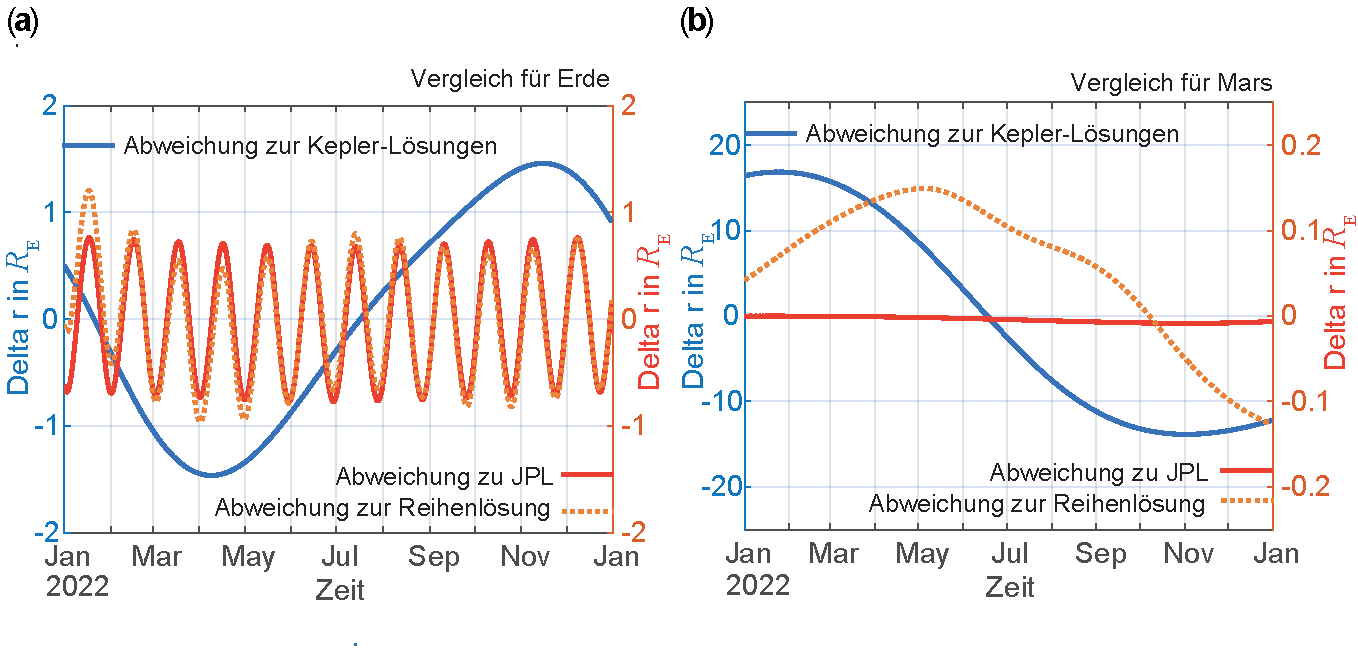
\includegraphics[width=\textwidth]{SonnensystemSimulation01.pdf}%
\caption[Sonnensystem-Simulation durch numerischen L�sung der Newtonschen Bewegungsgleichungen.]{Sonnensystem-Simulation durch numerischen L�sung der Newtonschen Bewegungsgleichungen. Abweichungen der L�sungen f�r die Bahn der Erde \fa und des Mars \fb von den Referenzdaten des JPL (\url{https://ssd.jpl.nasa.gov/horizons/}). Zum Vergleich sind auch die Abweichungen zur einfachen Kepler-L�sung und zur Reihenentwicklung nach der St�rungstheorie (\kap{Reihenentwicklung}) gezeigt.}%
\label{abb:hm_SonnensystemSimulation01}%
\end{figure}

In \figref{hm_SonnensystemSimulation02} zeigen wir die berechnete Bewegung des Schwerpunktes gegen�ber der Ausgangsposition. Eigentlich sollte dieser ja nach Definition in der Nulllage verbleiben. Die sehr kleine (man beachte die Achseneinteilung) systematische Drift resultiert aus der Tatsache, dass wir ja nicht �ber alle K�rper des Sonnensystems integriert haben. Es feheln ja etliche Monde, Kometen und Asteroiden. Die Gr��e der Drift ist f�r uns auch eine Aussage zur Genauigkeit der Integration.\\
%Es ist gar nicht so einfach die Frage zu beantworten, wie man f�r das Sonnensystem den Ursprung des Inertialsystems findet. Die IAU (\textit{International Astronomical Union}) hat �ber sehr pr�zise (\textit{Very Large Base Interferometry} - VLBI) Messungen
%von extra-galaktischen Quellen das sogenannte ICRF3-Koordinatensystem (International Celestial Reference Frame 3) definiert. Der Schwerpunkt dessen Sonnensystems (\textit{Solar System Bary Center}-SSBC) wird (nicht-relativistisch) definiert durch:
% 	\begin{align}
%		 \vec{R}_\text{SSBC}  = \lk \sum_j  m_i\vec{r}_i\rk \bigg/ \lk \sum_j m_j \rk \,, \label{eq:hm_PlanetenDGLSystem02}
%	\end{align}
%wobei �ber alle K�rper des Sonnensystems summiert wird.\\
%Der Leser wird m�glicherweise auch die Frage stellen, wie die hochgenauen Daten des JPL zustande kommen. Keine Frage, die Ephemeriden des JPL sind sehr gut, aber sie sind sicherlich nicht auf den Bruchteil eines Millimeters genau, obwohl sie mit so vielen Dezimalstellen angegeben werden. Zur Erstellung einer JPL Ephemeride weren mehrere Beobachtungsdaten (optische, Radardaten und Raumfahrzeug-Daten) mit dynamischen Modellen kombiniert, insofern ist die JPL Ephemeride eine "`gemischt beobachtete-gerechnete"' Ephemeride und hat sowohl als Messwert als auch Modellergebnis Ungenauigkeiten. Es wird eine optimale Anpassung entwickelt, um diese Fehler statistisch zu minimieren. Die resultierende Ephemeride ist mit einer stark reduzierten Unsicherheit verbunden. Obwohl die Vektordaten des JPL mit 16 Dezimalstellen ausgegeben werden, bedeutet das nicht, dass alle Ziffern physikalisch sinnvoll sind. Die gesamte Zahl der Stellen wird bei unseren Rechen- und Modellgenauigkeiten nat�rlich nicht ben�tigt. 

\begin{figure}[H]
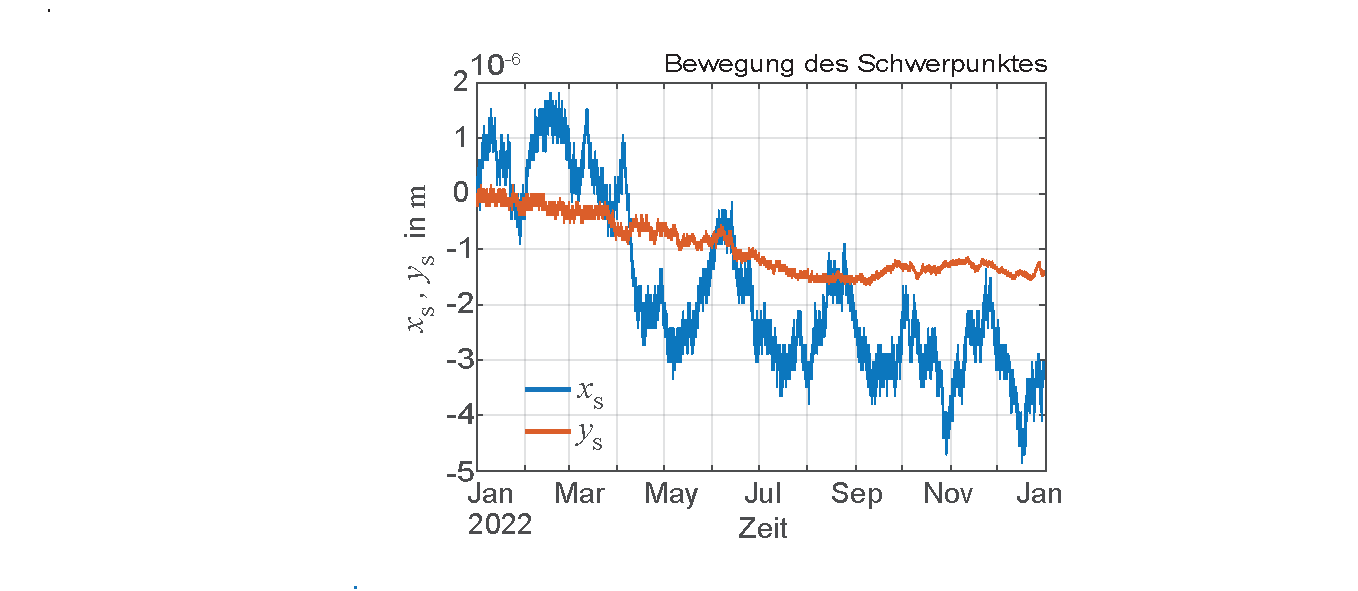
\includegraphics[width=\textwidth]{SonnensystemSimulation02.pdf}%
\caption[Sonnensystem-Simulation durch numerischen L�sung der Newtonschen Bewegungsgleichungen. Bewegung des Schwerpunktes.]{Sonnensystem-Simulation durch numerischen L�sung der Newtonschen Bewegungsgleichungen. Bewegung des Schwerpunktes.}%
\label{abb:hm_SonnensystemSimulation02}%
\end{figure}

In \figref{hm_SonnensystemSimulation03} vergleichen wir die numerischen L�sungen f�r \eqref{eq:hm_PlanetenDGLSystem01} f�r einen Zeitraum von 110 Jahren und \figref{hm_SonnensystemSimulation04} zeigt die Bewegung der Sonne aus der numerischen Integration von  \eqref{eq:hm_PlanetenDGLSystem01} relativ zum Baryzentrum des Sonnensystems (\mscr{}~ \mlhmref{SonnensystemSimulationLangeZeiten.m}) f�r den gleichen Zeitraum.

\begin{figure}[H]
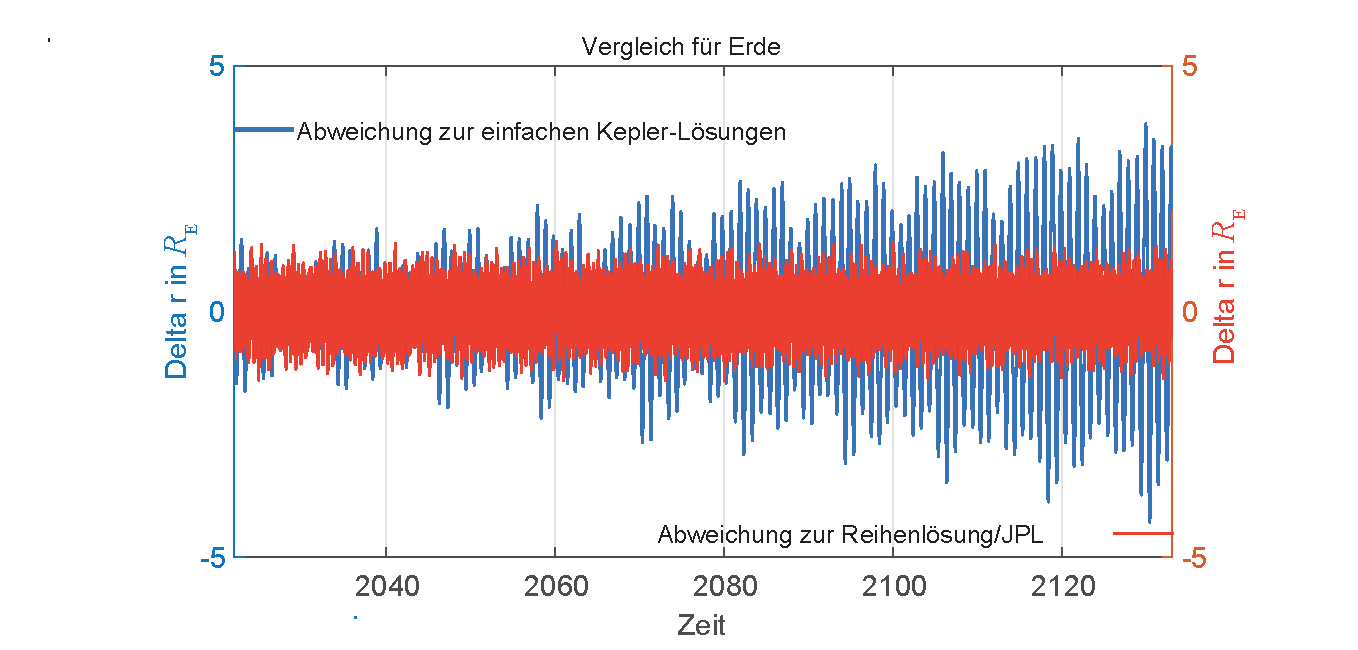
\includegraphics[width=\textwidth]{SonnensystemSimulation03.pdf}%
\caption[Sonnensystem-Simulation durch numerischen L�sung der Newtonschen Bewegungsgleichungen �ber lange Zeiten.]{Sonnensystem-Simulation durch numerischen L�sung der Newtonschen Bewegungsgleichungen �ber lange Zeiten. Abweichungen der L�sungen f�r die Bahn der Erde von den Referenzdaten des JPL (\url{https://ssd.jpl.nasa.gov/horizons/}). Zum Vergleich sind auch die Abweichungen der einfachen Kepler-L�sung zu den JPL Daten gezeigt.}%
\label{abb:hm_SonnensystemSimulation03}%
\end{figure}

\begin{figure}[H]
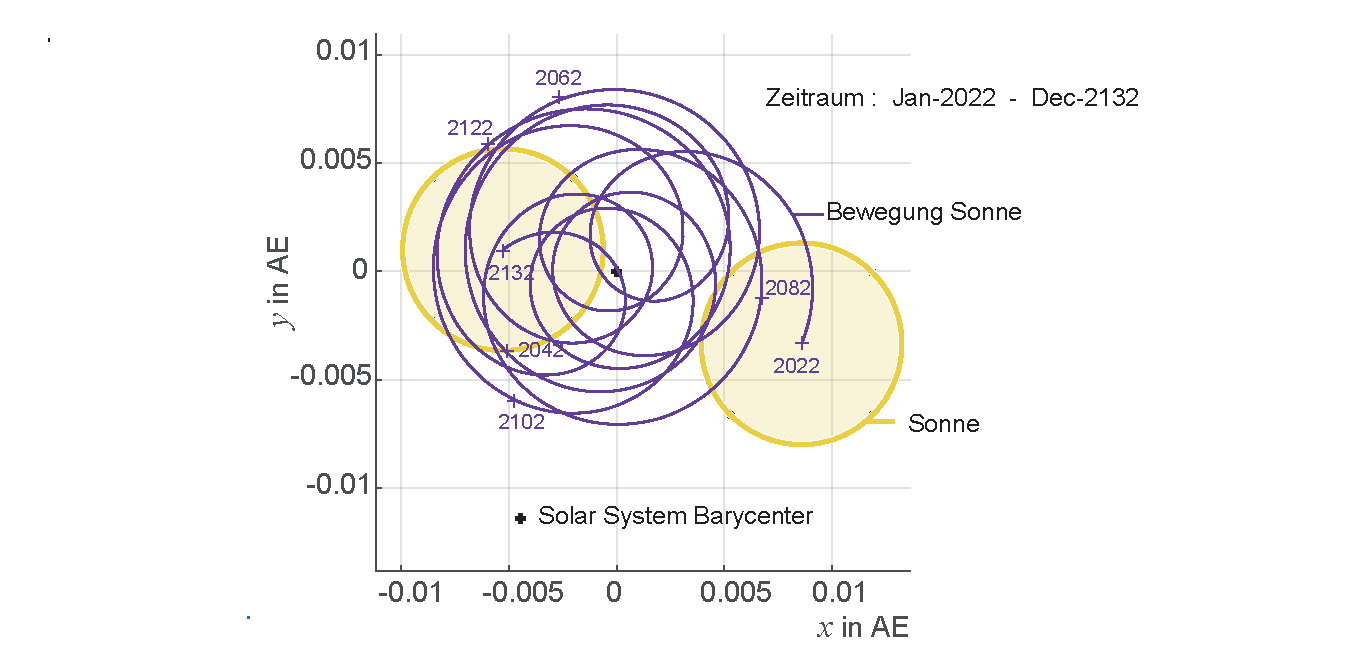
\includegraphics[width=\textwidth]{SonnensystemSimulation04.pdf}%
\caption[Sonnensystem-Simulation durch numerischen L�sung der Newtonschen Bewegungsgleichungen. Bewegung der Sonne im ICRF �ber 120 Jahre.]{Sonnensystem-Simulation durch numerischen L�sung der Newtonschen Bewegungsgleichungen. Bewegung der Sonne im ICRF �ber 110 Jahre. Die Anfangswerte $\vec{r}_i(t_0)$ und $\dot{\vec{r}}_i(t_0)$ haben wir uns wieder aus dem JPL-Webservice beschafft. Vergleiche dazu auch die Ergebnisse in \cite{Park2021}}%
\label{abb:hm_SonnensystemSimulation04}%
\end{figure}

Es ist gar nicht so einfach die Frage zu beantworten, wie man f�r das Sonnensystem den Ursprung des Inertialsystems findet. Die IAU ((\textit{International Astronomical Union})) hat �ber sehr pr�zise (\textit{Very Large Base Interferometry} - VLBI) Messungen
von extra-galaktischen Quellen das sogenannte ICRF3-Koordinatensystem (International Celestial Reference Frame 3) definiert. Der Schwerpunkt dessen Sonnensystems (\textit{Solar System Bary Center}-SSBC) wird (nicht-relativistisch) definiert durch:
 	\begin{align}
		 \vec{R}_\text{SSBC}  = \lk \sum_j  m_i\vec{r}_i\rk \bigg/ \lk \sum_j m_j \rk \,, \label{eq:hm_PlanetenDGLSystem03}
	\end{align}
wobei �ber alle K�rper des Sonnensystems summiert wird.\\
Der Leser wird m�glicherweise auch die Frage stellen, wie die hochgenauen Daten des JPL zustande kommen. Keine Frage, die Ephemeriden des JPL sind sehr gut, aber sie sind sicherlich nicht auf den Bruchteil eines Millimeters genau, obwohl sie mit so vielen Dezimalstellen angegeben werden. Zur Erstellung einer JPL Ephemeride weren mehrere Beobachtungsdaten (optische, Radardaten und Raumfahrzeug-Daten) mit dynamischen Modellen kombiniert, insofern ist die JPL Ephemeride eine "`gemischt beobachtete-gerechnete"' Ephemeride und hat sowohl als Messwert als auch Modellergebnis Ungenauigkeiten. Es wird eine optimale Anpassung entwickelt, um diese Fehler statistisch zu minimieren. Die resultierende Ephemeride ist mit einer stark reduzierten Unsicherheit verbunden. Obwohl die Vektordaten des JPL mit 16 Dezimalstellen ausgegeben werden, bedeutet das nicht, dass alle Ziffern physikalisch sinnvoll sind. Die gesamte Zahl der Stellen wird bei unseren Rechen- und Modellgenauigkeiten nat�rlich nicht ben�tigt. 
Sehr lesenswert zu diesem Thema ist f�r interessierte Leser die Referenz \cite{Park2021}.

\medskip \end{sol}

\textcolor{blue} {$\rightarrow$ zur} \probref{hm_Sonnensystem}.\\
\noindent\rule[1ex]{\textwidth}{0.5pt} \newpage

%-----------------------------------------------------------------------------------------------------------

\begin{sol}{prob:hm_Dreifachstern}\label{lsg:hm_Dreifachstern} %�bung29
\textbf{Dreik�rper-System - L�sung f�r 3 identische Massen} 
\begin{itemize}
	\item \textit{\textbf{Anordnung 1 - Achtf�rmige Trajektorien}}\\

Die Rechnungen sind im \mscr{}~ \mlhmref{DreiKoerperProblem01.m} hinterlegt.
\begin{figure}[H]
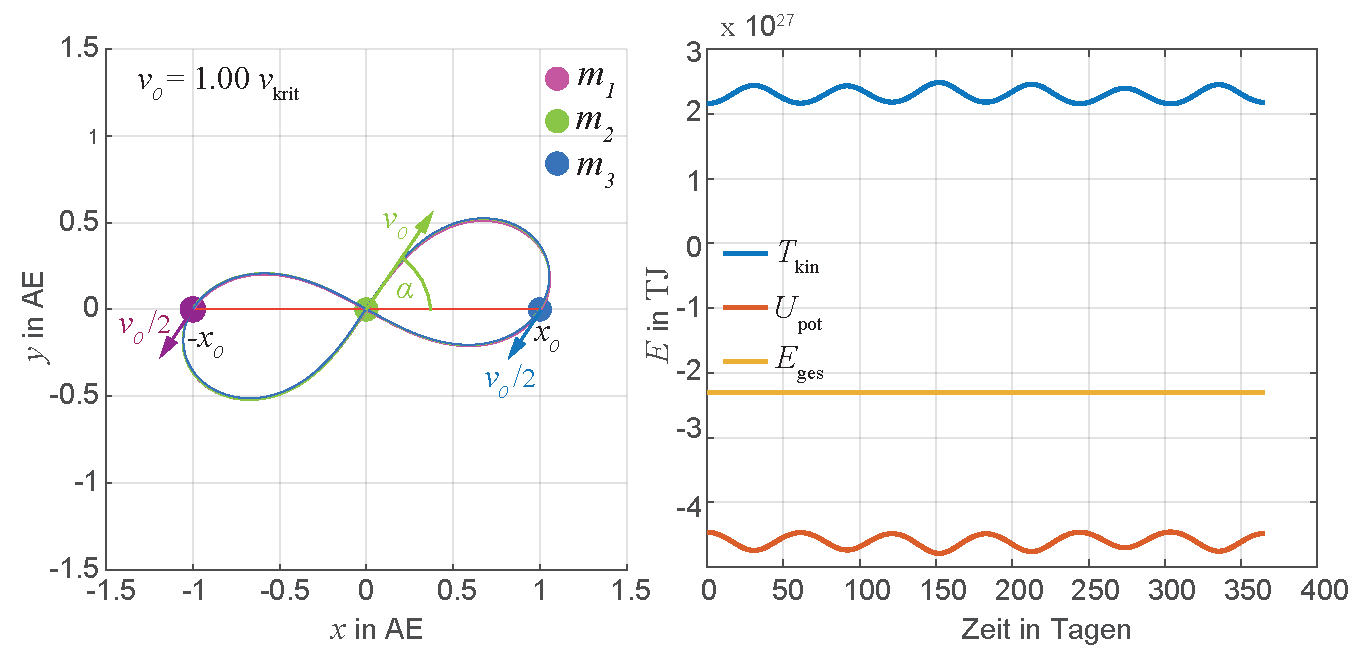
\includegraphics[width=0.9\textwidth]{DreiKoerperSystem01.pdf}%
\caption[Dreik�rperproblem mit Bewegung in Form einer Acht.]{Dreik�rperproblem mit Bewegung in Form einer Acht. Die Geschwindigkeit $v_0=v(t_0)$ ist genau der kritischen Geschwindigkeit $v_\text{krit} = 1.27\,\sqrt{G \, m / x_0}$, worin $2\,x(t_0)$ der Anfangsabstand der beiden �u�eren Massen $m_1$ und $m_3$ auf der $x$-Achse ist. Der Winkel von $\vec{v}_0$ zur $x$-Achse betr�gt $56.9\degree$ \cite{Moore1993, Chenciner2000}. Man erh�lt in diesem Fall stabile Bahnen.}
\label{abb:hm_DreiKoerperSystem01}%
\end{figure}
\begin{figure}[H]
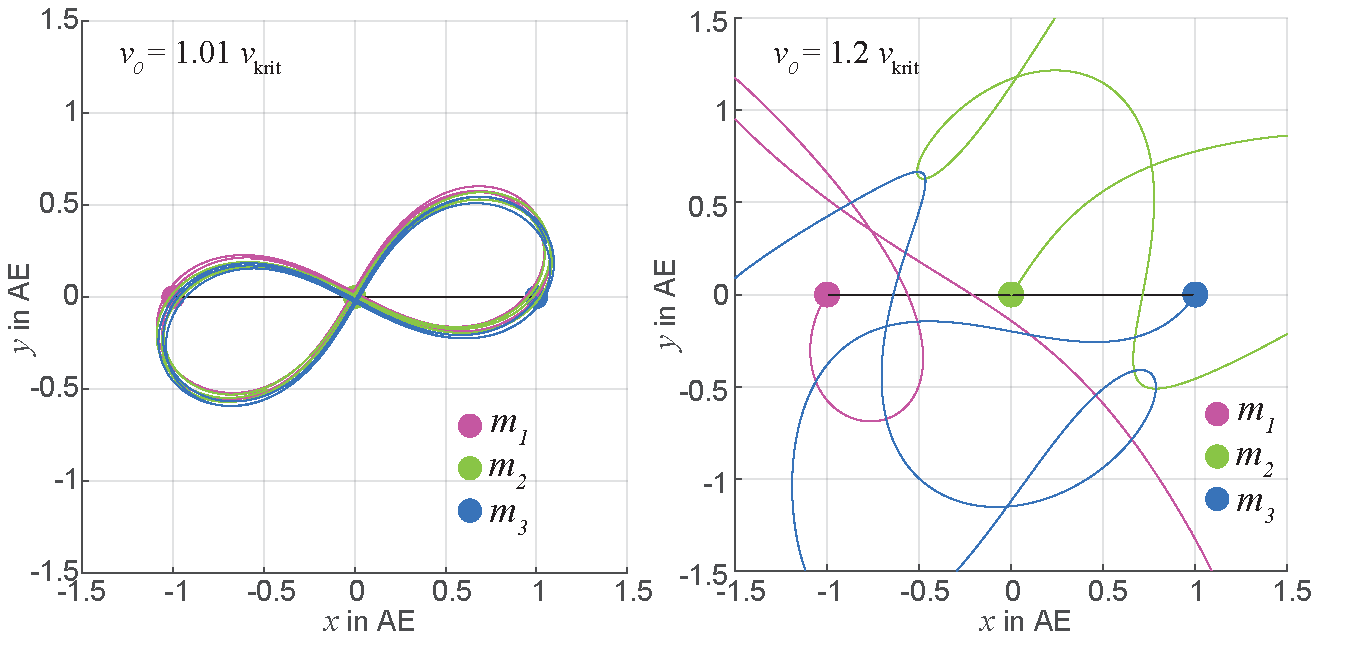
\includegraphics[width=0.9\textwidth]{DreiKoerperSystem02.pdf}%
\caption[Dreik�rperproblem mit Bewegung in Form einer Acht.]{Dreik�rperproblem mit Bewegung in Form einer Acht. Die Geschwindigkeit $v_0$ weicht 1\% (linkes Bild) \bzw 20\% von der der kritischen Geschwindigkeit $v_\text{krit} = 1.27\,\sqrt{(G \, m_0 / x_0)}$ ab. Man erkennt, dass man im linken Bild noch quasistabile Bahnen bekommt, im Fall rechts geht das System sehr schnell in einen chaotischen Zustand �ber.}
\label{abb:hm_DreiKoerperSystem02}%
\end{figure}
	
\newpage
	\item \textit{\textbf{Anordnung 2 - Gleichseitiges Dreieck}}\\
	
Wir k�nnen f�r diesen Fall auf Grund der Symmetrie leicht ableiten, dass die resultierende Kraft aus der Gravitation von den zwei anderen Massen auf die betrachtete betrachtete Masse (in \figref{hm_DreiKoerperSystemDreieck} $m_1$) jeweils in Richtung gemeinsamer Schwerpunkt zeigt und damit als Radialkraft die Massen auf eine kreisf�rmige Umlaufbahn zwingt. (Der Radius der Bahn ist dann gerade der Radius des Umkreises des gleichseitigen Dreiecks.)

\begin{figure}[H]
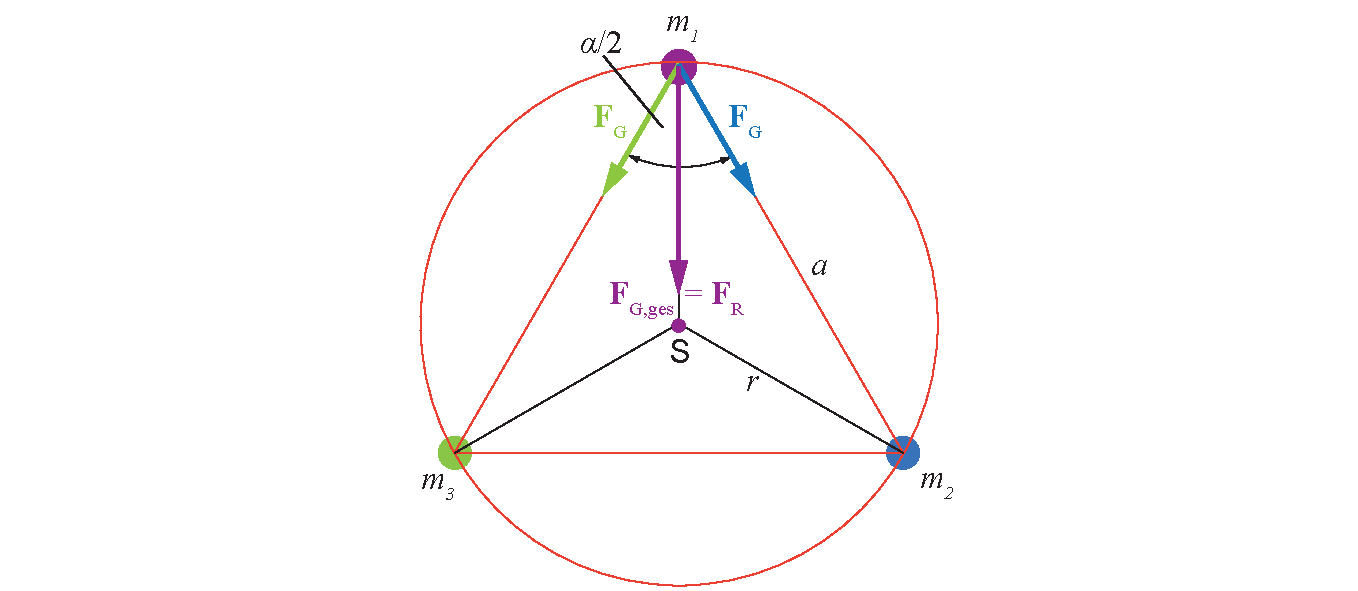
\includegraphics[width=0.9\textwidth]{DreiKoerperSystemDreieck.pdf}%
\caption[Geometrie des Dreik�rperproblem in Form eines gleichseitigen Dreiecks mit Drehung um Schwerpunkt. ]{Geometrie des Dreik�rperproblems in Form eines gleichseitigen Dreiecks mit Drehung um Schwerpunkt.}
\label{abb:hm_DreiKoerperSystemDreieck}%
\end{figure}

Wir wollen die Umlaufgeschwindigkeit berechnen. Dazu berechnen wir mit der Geometrie von \figref{hm_DreiKoerperSystemDreieck} die Gesamtkraft der Massen $m_2=m$ und $m_3=m$ auf die Masse $m_1=m$ zu:
\begin{align}
	\vec{F}_\text{G,ges} &=\frac{G m_1 m_2}{a^2}\,\begin{pmatrix} -\sin(\alpha/2) \\ \cos(\alpha/2 )\\ \end{pmatrix} + 
	        \frac{G m_1 m_3}{a^2}\,\begin{pmatrix} \sin(\alpha/2) \\ \cos(\alpha/2 )\\ \end{pmatrix} \nonumber \\
					&= 2\,\frac{G m^2}{a^2}\,\cos(\alpha/2)\, \veceY~~~~~\text{und mit}~\cos(\alpha/2)=\sqrt{3}/2~\text{, sowie}~d=r\,\sqrt{3} \,\nonumber \\
					&=\frac{G m^2}{\sqrt{3}\,r^2}\,\veceY\,.
	\label{eq:hm_DreiKoerperSystem01}				
\end{align}
Diese muss gleich der Radialkraft der Kreisbewegung sein, \dh:
\begin{align}
	\vec{F}_\text{R} &= \frac{m\,v^2}{r}\,\veceY = \frac{G m^2}{\sqrt{3}\,r^2}\,\veceY\,. 
	\label{eq:hm_DreiKoerperSystem02}				
\end{align}
Damit ergibt sich die Beziehung f�r die Geschwindigkeit: 
\begin{align}
	v = \sqrt{\frac{G\,m}{r\sqrt{3}}} = \sqrt{\frac{G\,m}{a}}\,.
	\label{eq:hm_DreiKoerperSystem03}				
\end{align}

F�r die Simulation im \mscr{}~ \mlhmref{DreiKoerperProblem02.m}\, nehmen wir einen Radius von einer Astronomischen Einheit und eine Masse der K�rper von zwei Sonnenmassen an. Wir erwarten daher eine Bewegung, die sich in der Zeitskala von Jahren abspielt. Das Programm simuliert 10-15 Jahre in Zeitschritten von einem Tag.
	
\begin{figure}[H]
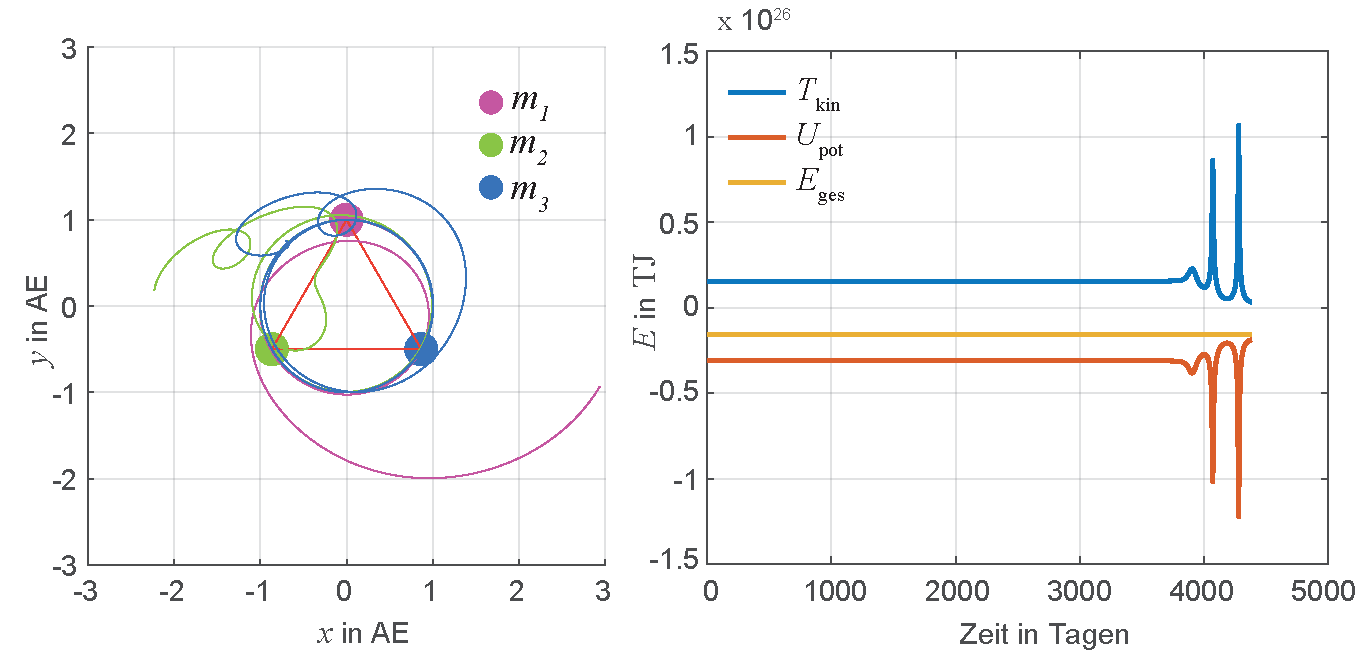
\includegraphics[width=0.9\textwidth]{DreiKoerperSystem03.pdf}%
\caption[Dreik�rperproblem in Form eines gleichseitigen Dreick mit Drehung um Schwerpunkt. ]{Dreik�rperproblem in Form eines gleichseitigen Dreiecks mit Drehung um Schwerpunkt. Man erkennt, dass das System nach einer anf�nglich stabilen Bahn in in einen chaotischen Zustand �bergeht. Dieser �bergangszeitpunkt (in unserem Fall in etwa bei \ca 10 Jahren) h�ngt stark von den Ungenauigkeiten der numerischen Rechnung ab. Man variiere dazu die Toleranzparameter in der options-Funktion des \odevf-Solvers.}
\label{abb:hm_DreiKoerperSystem03}%
\end{figure}
\end{itemize}

\medskip \end{sol}

\textcolor{blue} {$\rightarrow$ zur} \probref{hm_Dreifachstern}.\\
\noindent\rule[1ex]{\textwidth}{0.5pt} \newpage

%-----------------------------------------------------------------------------------------------------------

\begin{sol}{prob:hm_Tempel1_SwiftTuttle}\label{lsg:hm_Tempel1_SwiftTuttle} %�bung30
\textbf{Kometen im Sonnensystem -- Kollision mit der Erde?} \\ \\


Wir verweisen auf die \mscr e \mlhmref{KometenKollisionKepler.m}, \mlhmref{KometenKollisionSim.m} und \mlhmref{KometenKollisionJPL.m}.\\
Als Referenzdaten verwenden wir die Vektordaten aus \url{https://ssd.jpl.nasa.gov/horizons/} (\cite{JPL2020}).\\
Die Berechnung f�r die n�chste Ann�herung des Planeten im Jahr 2126 erfolgt �ber die Kepler-L�sung (\mlhmref{KometenKollisionKepler.m}), die numerische Integration der Bewegungsgleichungen mit den in \probref{hm_Sonnensystem} entwickelten Programmen und zum Vergleich �ber die JPL-Daten \mlhmref{KometenKollisionJPL.m}. Der Vergleich ergibt:
\begin{itemize}
	\item \textit{\textbf{Berechnung f�r 2126 �ber L�sung der Kepler-Gleichung}}\\
	
 Abstand Erdn�he :   0.91426408\,AE\,\,~ \bzw ~~ 1.3677e+08\,km\\
 Datum Erdn�he~~ :   24-Jun-2126\\

 Abstand Perihel :   0.95951616\,AE\,~~ \bzw ~~ 1.4354e+08\,km\\
 Datum Perihel~~ :   30-Apr-2126\\

\item \textit{\textbf{Berechnung f�r 2126 �ber numerische Integration der Bewegungsgleichungen \eqref{eq:hm_PlanetenDGLSystem01}}}\\ 

 Abstand Erdn�he :   0.15346854\,AE\,~~ \bzw ~~ 2.2959e+07\,km\\
 Datum Erdn�he~~ :   06-Aug-2126\\

 Abstand Perihel :   0.95630432\,AE\,~~ \bzw ~~ 1.4306e+08\,km\\
 Datum Perihel~~ :   12-Jul-2126\\

\item \textit{\textbf{Berechnungen des JPL}}\\ 

 Abstand Erdn�he :   0.1530400\,AE\,~~ \bzw ~~ 2.2894e+07\,km\\
 Datum Erdn�he~~ :   06-Aug-2126\\

 Abstand Perihel :   0.95416973\,AE\,~~ \bzw ~~ 1.4274e+08\,km\\
 Datum Perihel~~ :   14-Jul-2126\\

\end{itemize}

Die Ergebnisse der numerischen Integration der Bewegungsgleichungen �ber die Himmelsk�rper stimmen gut mit den JPL Daten �berein. Die einfache Kepler-Rechnung reicht offensichtlich nicht aus, der Komet wird auf seiner weiten Bahn offensichtlich von mehreren Himmelsk�rpern (insbesondere vom Jupiter) beeinflusst, so dass die einfache Zweik�rper-L�sung nicht mehr anwendbar ist. Nach unseren Rechnungen wird der Komet der Erde im Jahr 2026 zwar deutlich n�her kommen als in 1992, diese aber dennoch in einem Abstand von ca 20 Mio km passieren. Es droht also keine Kollisionsgefahr. Wir empfehlen aber dennoch Anfang 2125 mit neuen JPL Daten noch einmal nachzurechnen. In jedem Fall sollte der Komet sehr gut sichtbar werden.

Die Trajektorien von Swift-Tuttle sind f�r den Zeitraum von 110 Jahren \bzw in der Umgebung des Periheldurchgangs im Jahr 2126 in \figref{hm_SwiftTuttle01} dargestellt. \figref{hm_SwiftTuttle02} zeigt berechneten Trajektorien in der Umgebung des Periheldurchgangs im Jahr 2126 f�r die numerische Kepler-L�sung \bzw die  vollst�ndige Integration der Bewegungsgleichungen \eqref{eq:hm_PlanetenDGLSystem01} �ber "`alle"' Himmelsk�rper.

\begin{figure}[H]
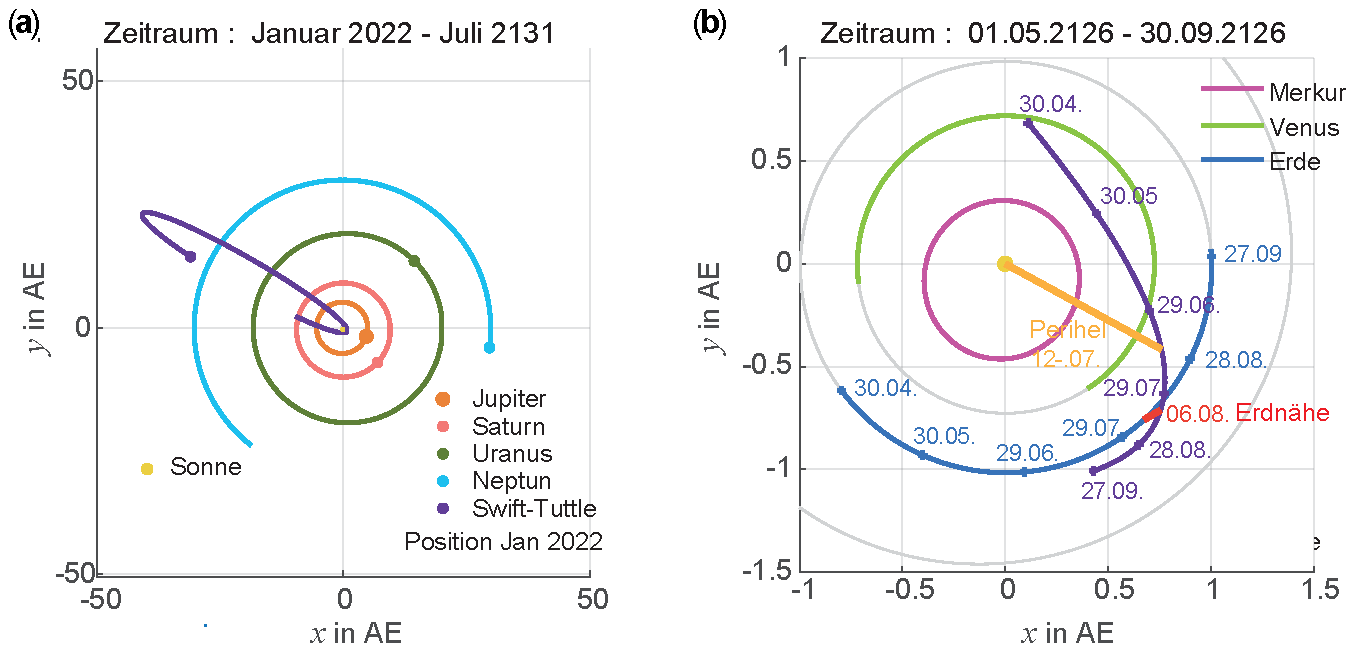
\includegraphics[width=\textwidth]{KometenKollision01.pdf}%
\caption[Trajektorien des Kometen Swift-Tuttle. ]{Berechnete Trajektorien des Kometen Swift-Tuttle. \fa Zeitraum 2022--2132  \fb Umgebung des Perihelduchgangs in 2126. Die Berechnung erfolgte durch numerische Integration der Bewegungsgleichungen \eqref{eq:hm_PlanetenDGLSystem01}.}
\label{abb:hm_SwiftTuttle01}%
\end{figure}

\begin{figure}[H]
\includegraphics[width=\textwidth]{KometenKollision02.pdf}%
\caption[Trajektorien des Kometen Swift-Tuttle zum Zeitpunkt Periheldurchgang in 2126.]{Berechnete Trajektorien des Kometen Swift-Tuttle zum Zeitpunkt des Periheldurchgangs in 2126. \fa Numerische Kepler-L�sung f�r den Kometen. \fb Numerische Integration der Bewegungsgleichungen \eqref{eq:hm_PlanetenDGLSystem01} �ber alle gr��eren Himmelsk�rper.}
\label{abb:hm_SwiftTuttle02}%
\end{figure}


\medskip \end{sol}

\textcolor{blue} {$\rightarrow$ zur} \probref{hm_Tempel1_SwiftTuttle}.\\
\noindent\rule[1ex]{\textwidth}{0.5pt} \newpage

%-----------------------------------------------------------------------------------------------------------

\begin{sol}{prob:hm_lichtlaufzeit}\label{lsg:hm_lichtlaufzeit} %�bung31
\textbf{Lichtlaufzeit, Unterschied $\ET-\UT$} \\ \\
Wir k�nnten zur L�sung der Aufgaben die verschiedenen \mscre zu den Kometen- und Asteroidenbahnen (\mlhmref{Kometenbahnen.m} und folgende) benutzen.
Wir wollen hier aber eine Absch�tzung machen und k�nnen uns daher das Leben etwas einfacher machen.
Wir nehmen an, dass Perihel und Perig�um in der ekliptikalen L�nge zusammenfallen und das beide in der Ekliptik liegen, \dh die ekliptikale Breite 0 ist.
Dies bedeutet, dass die Geschwindigkeit $v_\text{K}$ des Kometen maximal ist und ihre Richtung senkrecht zur Beobachtungsrichtung liegt.
Die Geschwindigkeit $v_\text{K}$ erh�lt man dann aus der vis-viva-Gleichung \eqref{eq:hm_vis-viva_polar} zu
	\[v_\text{K}^2=\mu_\text{G}\lk \frac{2}{q_\text{K}}-\frac{1}{a_\text{K}} \rk~,
\]
worin $q_\text{K}$ und $a_\text{K}$ der Perihelabstand bzw. die gro�e Halbachse der Kometenbahn sind.
Da f�r Kometen i.A. $a_\text{K}\gg q_\text{K}$ ist, gilt n�herungsweise
	\[v_\text{K} \approx \sqrt{\frac{2\mu_\text{G}}{q_\text{K}}} ~.
\]
Der Unterschied in astrometrischer und scheinbarer ekliptikaler L�nge ist dann gegeben durch:
	\[\Delta \lambda \approx \frac{v_\text{K} \Delta t}{q_\text{K}} = \frac{v_\text{K} (q_\text{K} /c)}{q_\text{K}} = \frac{1}{c} \sqrt{\frac{2\mu_\text{G}}{q_\text{K}}}.
\]
Unter der Annahme verschwindender ekliptikaler Breiten (siehe oben) und kleiner Zeiten $\Delta t$ k�nnen wir die Rektaszensions�nderung 
$\Delta \alpha$  aus der L�ngen�nderung  wie folgt 
	\[	\Delta \alpha = \Delta \lambda \cos \epsilon 
	\]
	berechnen, worin $\epsilon$ die Ekliptikschiefe ist.
        Wir erhalten dann f�r den Versatz auf der CCD in der Zwischenbildebene 
	\[\Delta x = \pm f \Delta \alpha ~~.
	\]
Das Bild des Kometen wird also dann im Bildfeld sein, wenn $\left| \Delta x \right| \leq 18 $ mm ist, wenn also gilt:
	\[\Delta x = \frac{f}{c} \sqrt{\frac{2\mu_\text{G}}{q_\text{K}}} \cos \epsilon \leq 18 \text{mm} 
	\]
Wir setzen f�r den Halleyschen Kometen (H) $q_\text{K} = 0.58 \text{AE}$ und f�r Neowise (N) $q_\text{K} = 0.29 \text{AE}$ ein und erhalten:
\begin{align*}
\Delta \alpha_\text{H} &= 0.58' ~~\text{ und } \Delta \alpha_\text{N} = 0.87'\\
v_\text{H}&= 55.3 \:\text{km/s} ~~\text{ und } ~v_\text{N} = 82.6\:\text{km/s}~\\
\Delta x_\text{H} &= 0.43\:\text{mm} ~~\text{ und } ~\Delta x_\text{N} = 0.63\:\text{mm}~,
\end{align*}
was merklich ist (30 Bogensekunden), aber noch deutlich innerhalb des Bildfeldes.
Folglich w�rde auch bei Benutzung von UT anstelle ET, was einer Lichtlaufzeit von ca. 1 min entspricht, ebenfalls ein messbarer Positionsfehler von ca. 6 bis 8 Bogensekunden entstehen, aber der Komet ebenfalls gut im Bildfeld sein.
F�r genaue Astronomie reicht die Nichtber�cksichtigung von $\Delta T$ nat�rlich nicht aus.
Wir berechnen jetzt die Zeit $\Delta t_\text{G}$ in der der Komet aus dem Bildfeld des mitgef�hrten Teleskops herauswandert.
Es gilt:
\[\Delta \alpha_\text{G} = \frac{18\:\text{mm}}{f} = \frac{v_\text{K} \Delta t_\text{G}}{\left| q_\text{K}-a_\text{earth}\right|} ~
\]
woraus f�r die beiden Zeiten 148 min bzw. 175 min folgt.
Das hei�t, dass selbst bei perfekt mitgef�hrtem Teleskop die Kometen nach zwei bis drei Stunden aus dem Teleskopbildfeld "`herauswandern"'.
Man kann also die Eigenbewegung der Kometen in einer Nacht sehr gut beobachten.
Die Rechnungen k�nnen nat�rlich auch im Detail mit dem \mscr~\mlhmref{Kometenbahnen.m} nachvollzogen werden. \\
\medskip \end{sol}
\textcolor{blue} {$\rightarrow$ zur} \probref{hm_lichtlaufzeit}.\\
\noindent\rule[1ex]{\textwidth}{0.5pt} \newpage

%-----------------------------------------------------------------------------------------------------------
\newpage
%%%-----------------------------------------------------------------------------------------------------------
\subsection{�bungen zu Gezeiten}

%-----------------------------------------------------------------------------------------------------------

\begin{sol} {prob:hm_rochelimit} \label{lsg:hm_rochelimit} %�bung32
\textbf{Zur Herleitung des Roche-Limits.}\\ \\

Wir benutzen Abb. 1.14 (Band I), wobei im Bild Sonne/Mond durch Jupiter ersetzt werden muss und die Erde durch den Kometen.
Ebenso ersetzen wir $m \rightarrow m_\text{K},\,r \rightarrow d,\, R_\text{E} \rightarrow R_\text{K}.$
Wir betrachten den Punkt ($x=0$, $y=0$, $z=-R_\text{K}$). Dann wird aus Gleichung (1.103) aus Band I:\footnote{Alternativ kann man nat�rlich auch direkt Gleichung (1.103) aus Band I mit $\theta = 0$ \bzw $\theta = \pi$ benutzen.} 

\begin{align}
    \vec{g}_z = -\frac{2G\,m_\text{J}}{d^3}\,R_\text{K}\,\vec{e}_z \,. \label{eq:hm_lsgroche02}
\end{align}
\begin{align}
    g_z = -g_\text{Gez,V} &= g_0\,\frac{R_\text{E}}{r}\lk 3\cos^2\theta-1\rk = \frac{3}{2}\,g_0\,\frac{R_\text{E}}{r}\lk \cos2\theta+\frac{1}{3}\rk \,. 
\end{align}

Andersereits wirkt an dem Punkt die (Selbst-) Gravitation des Kometen:
\begin{align}
    g_\text{K} = + \frac{G\,m_\text{K}}{R_\text{K}{}^2}\,\vec{e}_z \,. \label{eq:hm_lsgroche03}
\end{align}
von \eqref{eq:hm_lsgroche02} und \eqref{eq:hm_lsgroche03} ergibt die effektiv wirkende Gravitationsbeschleunigung $g_\text{eff}$ auf den Kometen:
\begin{align}
    g_\text{eff} = \frac{G\,m_\text{K}}{R_\text{K}{}^2}\,\lk 1-2\,\frac{m_\text{J}}{m_\text{K}}\,\frac{R_\text{K}{}^3}{d^3}\rk \,, \label{eq:hm_lsgroche04}
\end{align}
welche f�r
\begin{align}
    d = r_\text{R} = \sqrt[3]{2\,\frac{m_\text{J}}{m_\text{K}}}\,R_\text{K} \label{eq:hm_lsgroche05}
\end{align}
verschwindet. Das ist genau das Roche-Limit und der Komet wir bei diesem Abstand zerrissen. \\
F�r $m_\text{J}/m_\text{K}$ k�nnen wir auch schreiben 
\begin{align}
    \frac{m_\text{J}}{m_\text{K}} = \frac{\varrho_\text{J}}{\varrho_\text{K}}\,\frac{R_\text{J}{}^3}{R_\text{K}{}^3}\,,\label{eq:hm_lsgroche06}
\end{align}
womit aus \eqref{eq:hm_lsgroche05} folgt
\begin{align*}
    r_\text{R} = \sqrt[3]{2}\,\sqrt[3]{\frac{\varrho_\text{J}}{\varrho_\text{K}}}\,R_\text{J}\,.
\end{align*}
Mit den bekannten Werten $\varrho_\text{K} = \SI{500}{kg\per\cubic\metre}$, $\varrho_\text{J} = \SI{1333}{kg\per\cubic\metre}$ und $R_\text{J} = \SI{69911}{\km}$ ergibt sich
\begin{align*}
    r_\text{R,K} = 1.26\, \sqrt[3]{\frac{1.33}{0.5}}\,\SI{69911}{km} \approx \SI{122000}{\km}\,,
\end{align*}
was gut mit den beobachteten ca. $\SI{100000}{\km}$ zusammen passt.
Die Formel \eqref{eq:hm_lsgroche05} \bzw \eqref{eq:hm_lsgroche06} ergibt eher zu kleine Werte, da 
\begin{enumerate}
    \item [a)]
    der Komet als komplett fest und 
    \item [b)]
    auch dauerhaft kugelf�rmig bis zum Zerrei�en angenommen wurde. Tats�chlich wird sich dieser aber elongiert verformen und auch zumindest teilweise in einen fluiden Zustand �bergehen.  
\end{enumerate}
Der Radius der Hill-Sph�re des Jupiters betr�gt (\vgl \probref{hm_hill_sphere}) ca. $\SI{0.35}{}\,\mathrm{AE}$, also ein vielfaches des Roche-Limits. Himmelsk�rper k�nnen sich also lange im \anf{Einflussbereich} des Jupiters bewegen, bevor sie zerrissen werden. In \figref{hm_RocheLimit} haben wir die Hill-Sph�ren und die Roche-Limits f�r unser Sonnensystem graphisch dargestellt.
Wir verweisen auf \mlhmref{RocheLimit.m}.

\begin{table}[H] \caption{Roche-Limit und Hill-Sph�re in unserem Sonnensystem.}
\hspace{0.5cm}
\begin{tabular}{|R{1.25cm}|R{1.75cm}|R{1.25cm}|R{2cm}|R{1.75cm}|R{1.75cm}|R{1.5cm}|R{1.75cm}|}
\hline
\rule{0pt}{3pt}& & & & & & & \\
Planet   ~ & $a_\text{P}$ ~\linebreak in AE   ~ & $\varrho_\text{P}$ ~\linebreak in $\SI{}{\kg\per\metre\cubed}$ ~& Radius $R_\text{P}$ ~\linebreak in km  ~ & $m_\text{P}$ ~\linebreak in kg   ~& Roche-Limit ~\linebreak  in $\SI{}{\km}$ ~& Hill-Sph�re ~\linebreak in AE ~& Hill-Sph�re ~\linebreak in $\SI{}{\km}$ ~ \\
\rule{0pt}{3pt}& & & & & & & \\
\hline
\rule{0pt}{3pt}& & & & & & &\\
\rule{0pt}{6pt}Merkur  ~& $\SI{0.38709 }{}$    ~& $\SI{5 427}{}$ ~& $\SI{2 439}{}$ ~& $\SI{3.302e23}{}$ ~&  $\SI{6 806}{}$              ~& $\SI{0.001 }{}$            ~& $\SI{2.21e5 }{}$         ~\\
\rule{0pt}{6pt}Venus   ~& $\SI{0.72333}{}$     ~& $\SI{5 243}{}$ ~& $\SI{6 052}{}$  ~& $\SI{4.869e24}{}$ ~&  $\SI{16 691 }{}$            ~& $\SI{0.007}{}$             ~& $\SI{1.01e6  }{}$        ~\\
\rule{0pt}{6pt}Erde    ~& $\SI{1.00000}{}$     ~& $\SI{5 515}{}$ ~& $\SI{6 371}{}$  ~& $\SI{5.974e24}{}$ ~&  $\SI{17 869}{}$             ~& $\SI{0.010}{}$             ~& $\SI{1.50e6 }{}$         ~\\
\rule{0pt}{6pt}Mars    ~& $\SI{1.52366 }{}$    ~& $\SI{3 933}{}$ ~&$\SI{3 389}{}$   ~& $\SI{6.419e23}{}$ ~&  $\SI{8 494 }{}$             ~& $\SI{0.007 }{}$            ~& $\SI{1.08e6}{}$          ~\\
\rule{0pt}{6pt}Jupiter ~& $\SI{5.20336}{}$     ~& $\SI{1 326}{}$ ~& $\SI{69 911}{}$ ~& $\SI{1.899e27}{}$ ~&  $\SI{121 929  }{}$          ~& $\SI{0.355 }{}$            ~& $\SI{5.32e7 }{}$         ~\\
\rule{0pt}{6pt}Saturn  ~& $\SI{9.53707}{}$     ~& $\SI{687}{}$  ~& $\SI{58 233}{}$ ~& $\SI{5.685e26}{}$ ~&  $\SI{81 571}{}$             ~& $\SI{0.436 }{}$            ~& $\SI{6.52e7 }{}$         ~\\
\rule{0pt}{6pt}Uranus  ~& $\SI{19.19126}{}$    ~& $\SI{1 270}{}$ ~& $\SI{25 362}{}$ ~& $\SI{8.685e25}{}$ ~&  $\SI{43 601}{}$             ~& $\SI{0.469}{}$             ~& $\SI{7.01e7 }{}$         ~\\
\rule{0pt}{6pt}Neptun  ~& $\SI{30.06896}{}$    ~&$\SI{1 638 }{}$ ~& $\SI{24 622}{}$ ~& $\SI{1.026e26}{}$ ~&  $\SI{46 076}{}$             ~& $\SI{0.776 }{}$            ~& $\SI{1.16e8 }{}$         ~\\
\rule{0pt}{6pt}Pluto   ~& $\SI{39.48169}{}$    ~& $\SI{1 854}{}$ ~& $\SI{1 185}{}$  ~& $\SI{1.303e22}{}$ ~&  $\SI{2 311}{}$              ~& $\SI{0.051 }{}$            ~& $\SI{7.66e6}{}$          ~\\
\rule{0pt}{3pt}& & & & & & &\\
\hline
\end{tabular} \label{tab:hm_rochelimit}
\end{table}


\begin{figure}[H]
	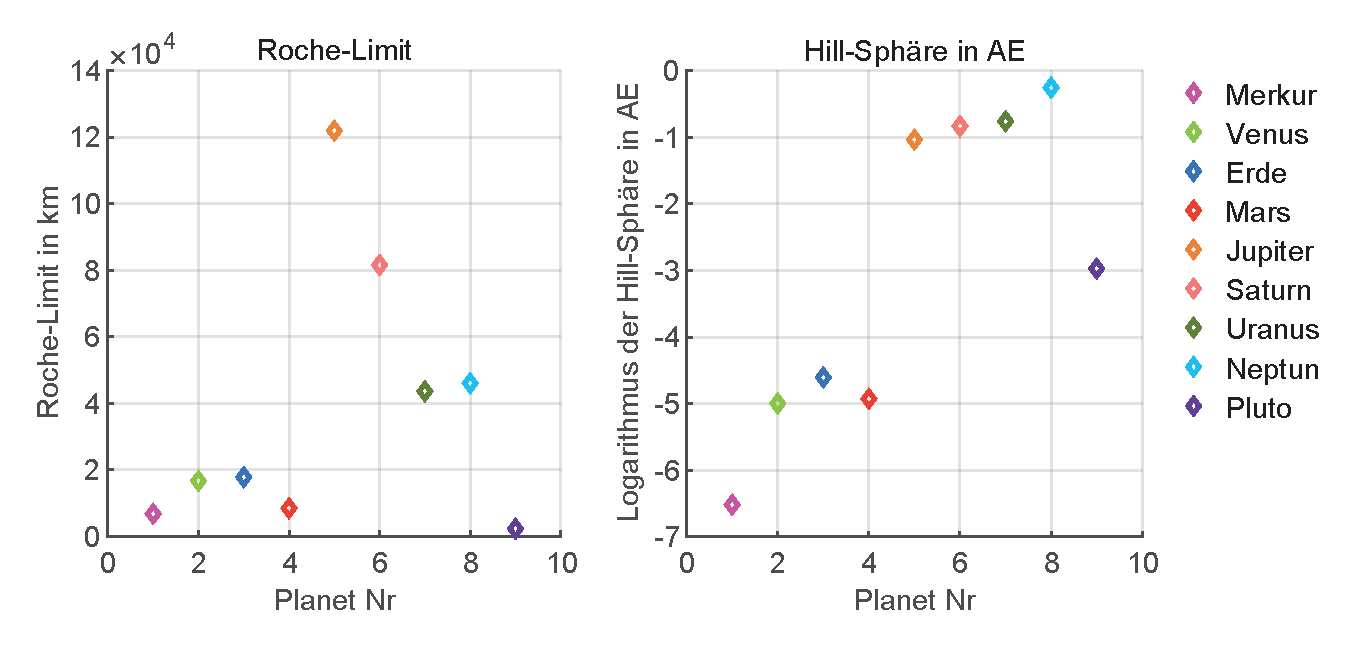
\includegraphics[width=\textwidth]{RocheLimit.pdf} 
	\caption[Vergleich Roche-Limit und Hill-Sph�re f�r unser Planetensystem.]{Vergleich Roche-Limit und Hill-Sph�re f�r unser Planetensystem.}
	\label{abb:hm_RocheLimit}
\end{figure}


\medskip \end{sol}
\textcolor{blue} {$\rightarrow$ zur} \probref{hm_rochelimit}.\\
\noindent\rule[1ex]{\textwidth}{0.5pt} \newpage


%-----------------------------------------------------------------------------------------------------------

\begin{sol} {prob:hm_gezeiten01} \label{lsg:hm_gezeiten01} %�bung33
\textbf{Tidenhub in einem Wasserglas}\\ \\

Wir betrachten \figref{hm_lsggezeiten01}. 
\begin{figure}[H]
	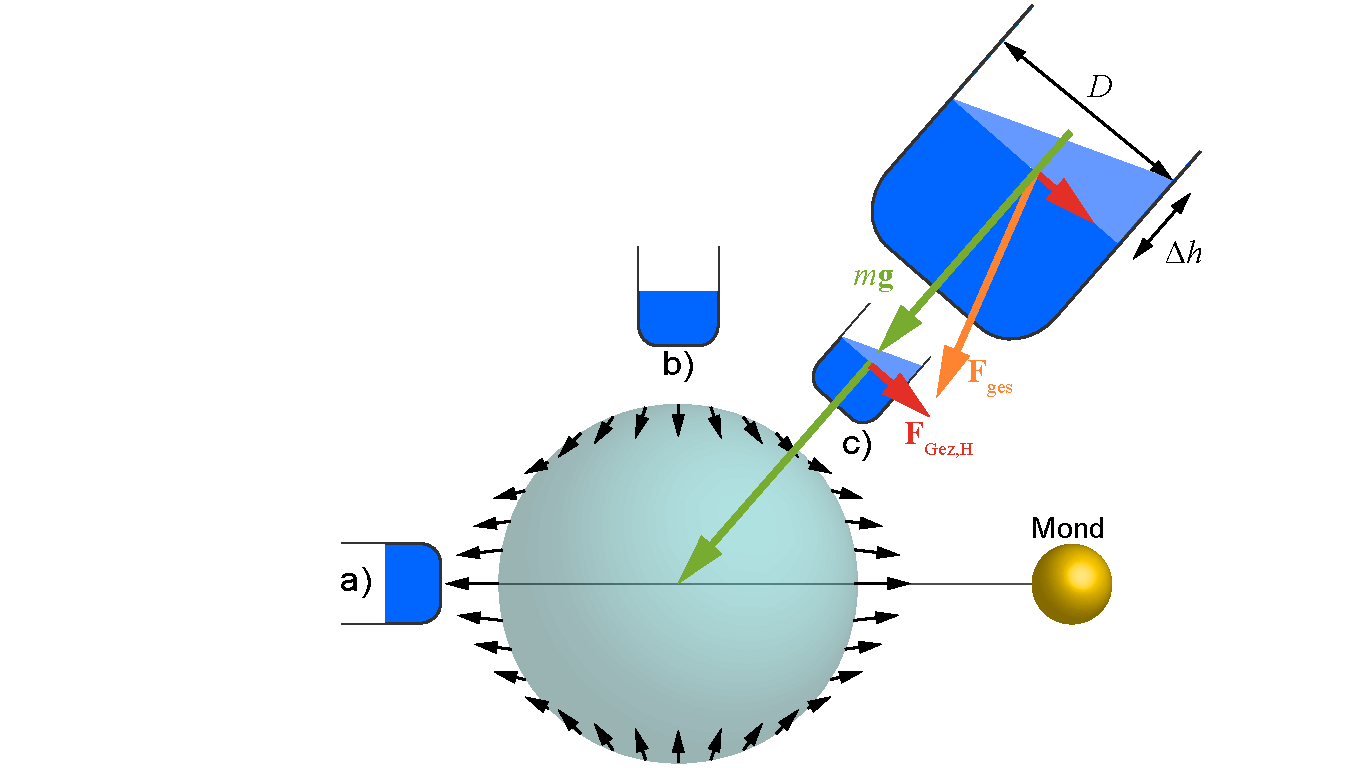
\includegraphics[width=\textwidth]{GezeitenWasserglas.pdf} 
	\caption{Gezeiten im Wasserglas}
	\label{abb:hm_lsggezeiten01}
\end{figure}
Nach der Gleichgewichtstheorie stellt sich die Wasseroberfl�che immer senkrecht zur resultierenden Gesamtschwerkraft $\vec{F}_\text{ges}$ ein. Der Tidenhub $\Delta h$ entspricht dann der Differenz der Wasserh�hen an beiden Ufern (\bzw dem R�ndern des Wasserglases). \\

Wir wollen nur die Wirkung des Mondes betrachten. Steht dieser im Zenit (Nadir) oder am Horizont, so bewirkt die resultierende Gesamtkraft keine Ver�nderung der Oberfl�che (Fall a,b). Im Fall c beginnt das Wasser durch Flie�en sich auszugleichen. \\
Der Tidenhub ergibt sich dann N�herungsweise zu:
\begin{align*}
    \Delta h = D\,\frac{F_\text{Gez,H}}{mg}\,.
\end{align*}
Wir wissen, dass $F_\text{Gez}/mg \approx \SI{e-7}{}$ ist, so dass folgt:
\begin{align*}
    \Delta h  &= \SI{e-8}{\metre} = \SI{10}{\nano\metre} ~~~~ \text{(Wasserglas)}, \\
    \Delta h  &= \SI{e-7}{}\cdot 5\cdot \SI{e4}{\metre} = 5\cdot \SI{e-3}{\metre} = \SI{5}{\mm} ~~~~ \text{(Bodensee)}.
\end{align*}

\newpage
Den Effekt im Glas k�nnte man im perfekt isolierten Labor ja noch interferometrisch messen, in der Badewanne oder aber im Bodensee wird er gegen�ber anderen Effekten verschwindend gering. 
In der Tat wurde die Wirkung von Gezeiten in $\SI{150}{\metre}$ langen Wasserrohren bereits 1914-1917 von Michelson\footnote{Albert Abraham Michelson (1852 -- 1931) war ein US-amerikanischer Physiker deutscher Herkunft. Er war einer der angesehensten Experimentalphysiker und wurde vor allem durch das nach ihm benannte Michelson-Interferometer bekannt. Er erhielt 1907 als erster US-Amerikaner den Nobelpreis f�r Physik.}\indexp{Michelson, Albert Abraham} und Mitarbeitern experimentell vermessen \cite{Michelson2014}.

\medskip \end{sol}
\textcolor{blue} {$\rightarrow$ zur} \probref{hm_gezeiten01}.\\
\noindent\rule[1ex]{\textwidth}{0.5pt} \newpage



%-----------------------------------------------------------------------------------------------------------

\begin{sol} {prob:hm_gezeiten02} \label{lsg:hm_gezeiten02} %�bung34
\textbf{Bewegung des Erdk�rpers im Erde-Mond-System.}\\

Der Umlauf von Erde und Mond um ihren gemeinsamen Schwerpunkt erzeugt oft Verwirrung. Oft wird argumentiert, dass die Erde dem Mond immer die gleich Seite zuwendet. Das ist aber falsch.
In der Realit�t f�hren alle Punkte der Erde eine Umlaufbewegung mit dem gleichen Radius aus und erfahren dabei eine gleiche Tr�gheitskraft (Fliehkraft), die immer vom Mond weg gerichtet ist. Jeder Punkt der Erde hat dabei sein eigenes Umlaufzentrum. Nur das gesamte System Erde-Mond f�hrt eine Bewegung um den Schwerpunkt S aus, nicht aber ein einzelner Massepunkt der Erde (Erde ist ja ein starrer K�rper).
Die \matlab{} Computersimulation \mlhmref{UmlaufErdeMond.m} zeigt in \figref{hm_lsggezeiten02}, dass jeder Punkt der Erde innerhalb eines synodischen Monats eine solche Kreisbewegung um sein jeweils eigenes "`Umlaufzentrum"' ausf�hrt. Dabei wurde die Situation f�r die �quatorebene dargestellt und angenommen, dass der Mond sich in der �quatorebene um den gemeinsamen Schwerpunkt S bewegt. Die Bewegung von zwei um $180\degree$ versetzten Punkten (T,B) in der �quatorebene sowie des Erdmittelpunktes im Lauf eines Monats sind dargestellt.

\newpage
\begin{figure}[H]
	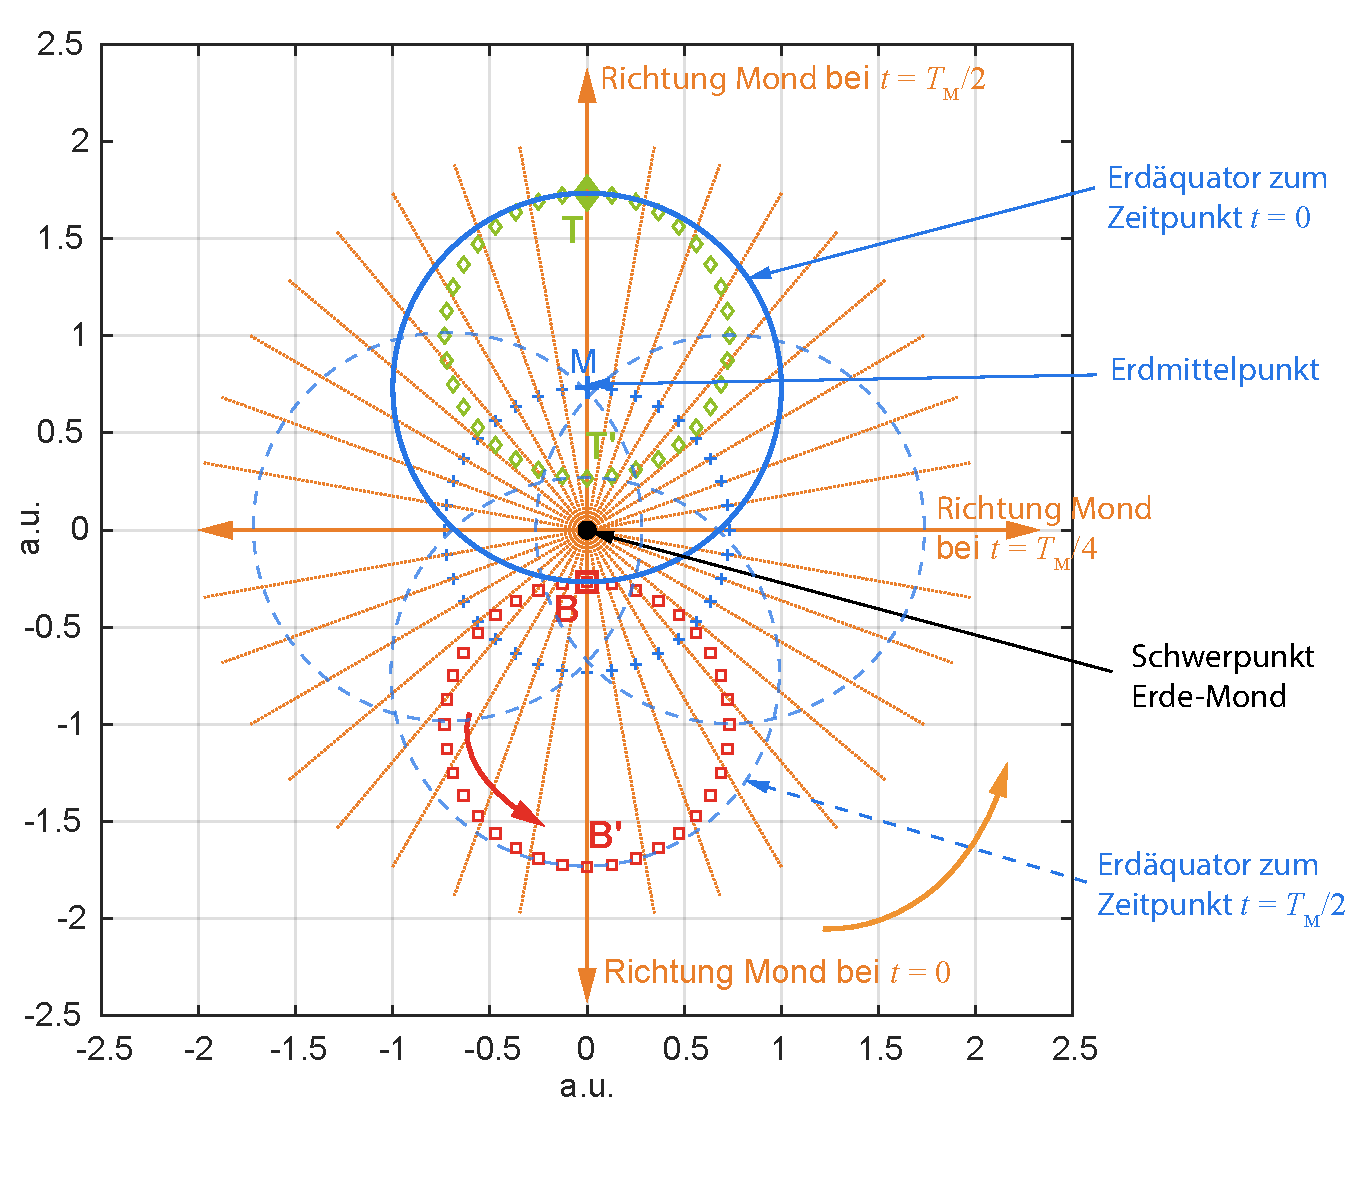
\includegraphics[width=\textwidth]{UmlaufErdeMond.pdf} 
	\caption[Bewegung von verschiedenen Punkten im Erde-Mond-System.]{Bewegung von verschiedenen Punkten der Erde bei einem Umlauf im Erde-Mond-Schwerpunkt-KOS. M ist der Erdmittelpunkt, T ein Punkt auf dem �quator, der bei $t=0$ auf der dem Mond abgewandten Seite liegt, T' der gleiche Punkt auf dem �quator, der bei $t=T_\text{M}/2$ dann auf der dem Mond zugewandten Seite liegt. F�r die Punkte B und B' gilt das Gleiche umgekehrt. $T_\text{M}$ ist die Umlaufzeit des Mondes um die Erde, die Erdrotation ist in dieser Betrachtung nicht ber�cksichtigt.}\label{abb:hm_lsggezeiten02}
\end{figure}
\end{sol}

\textcolor{blue} {$\rightarrow$ zur} \probref{hm_gezeiten02}.\\
\noindent\rule[1ex]{\textwidth}{0.5pt} \newpage

%-----------------------------------------------------------------------------------------------------------

\begin{sol} {prob:hm_gezeiten03} \label{lsg:hm_gezeiten03} %�bung35
\textbf{Newtonsche Gleichgewichtstheorie}\\ 

Abstand zwischen zwei Hochwassern und Tidenhub bei verschiedenen Deklinationen:
\begin{itemize}
	\item \textit{Abstand zwischen zwei Hochwassern }\\
			Aus der Dauer des synodischen Monats von $27.32 \mathrm{d}$ (Sonnentagen) ergibt sich eine mittlere Bewegung\index{Bewegung!mittlere} des Mondes von $n_\text{M} = 13.177\degree \mathrm{d}^{-1}$. An einem Sonnentag hat sich die Erde im Mittel um etwa 
	\[			360\degree \lk 1 + \frac{1\,\mathrm{d}}{365.25\,\mathrm{d}}\rk 
	\]
			weiter bewegt, was einer Bewegung von $n_\text{E} = 360.986\degree \mathrm{d}^{-1}$ entspricht. \\
			Wir wollen die zus�tzliche Zeit $\Delta T$ bestimmen, die verstreicht bis der Mond wieder im Meridian steht, \dh:
			\begin{align*}
					n_\text{E}\,\Delta T -360\degree &= n_\text{M} \, \Delta T \\
					\rightarrow ~~~~\Delta T = \frac{360\degree}{n_\text{E}-n_\text{M}} &= \frac{360\degree}{360.986\degree -13.177\degree}\, \mathrm{d} = \frac{360\degree}{347.809\degree}\, \mathrm{d} = 1.035 \mathrm{d} = \SI{24}{\hour}\,\SI{50}{\min}\,\SI{24}{\second}
			\end{align*}
			Hochwasser wird also im Mittel aller $\Delta T/2 = \SI{12}{\hour}\,\SI{25}{\min} $ eintreten.
			\begin{figure}%
			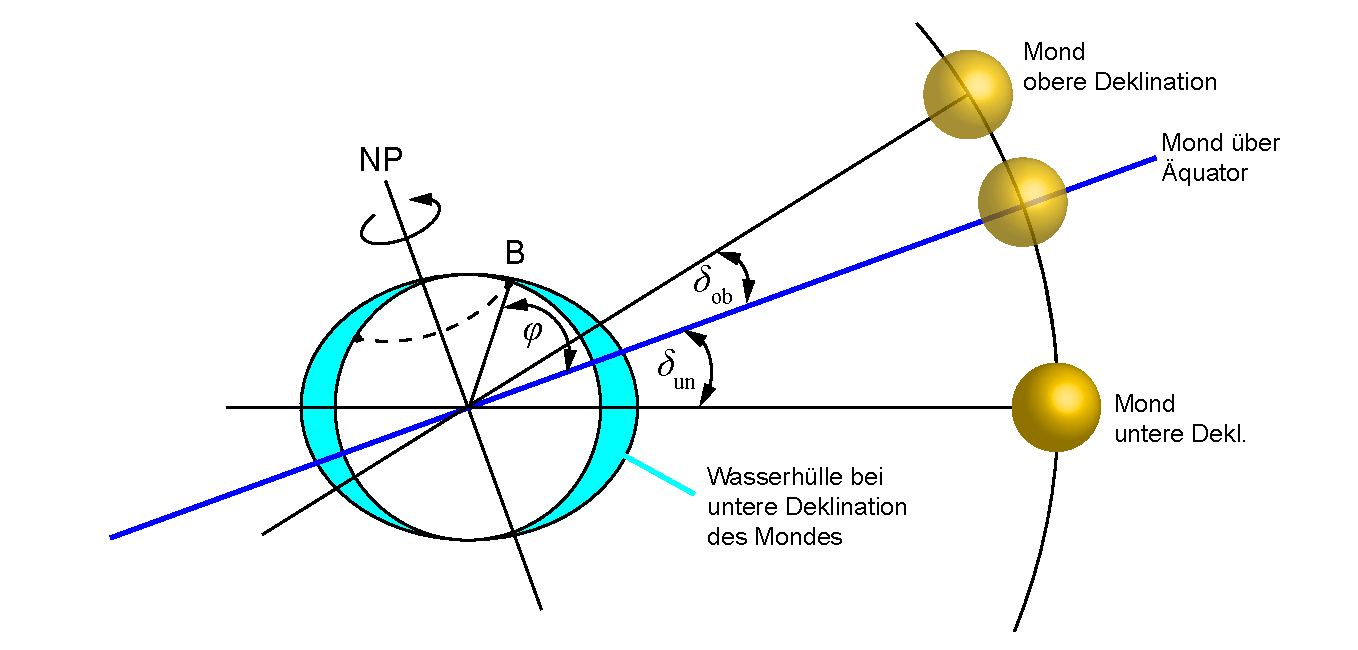
\includegraphics[width=\textwidth]{NewtonTheorieGez.pdf}%
			\caption{Anwendung der Newtonschen Gleichgewichtstheorie der Gezeiten}
			\label{abb:hm_lsggezeiten03}
			\end{figure}\newpage
	\item \textit{Tidenhub als Funktion der geographischen Breite }\\
	Man erkennt aus \figref{hm_lsggezeiten03}, dass die Tidenh�be f�r zwei aufeinander folgenden HW unterschiedlich hoch sind
	\item \textit{Tidenhub am �quator}\\
	Man erkennt aus \figref{hm_lsggezeiten03}, dass die Tidenh�be maximal sind, wenn der Mond die Deklination 0 hat. Ansonsten gibt es auch hier zwischen zwei aufeinander folgenden Hochwassern Unterschiede. Aus der Gezeitentabelle von Diego Garcia lesen wir heraus:
		\begin{enumerate}
		\item Sehr sch�n sind die Springtiden zum Vollmond und Neumond zu erkennen. (9.12. und 23.12.). Allerdings betr�gt die Differenz von HWH und NWH  \ca 250 cm, deutlich mehr als nach der Newtonschen Theorie zu erwarten w�re. Da zum Zeitpunkt des Vollmondes seine Deklination \ca $-10\degree$ betr�gt, die der Sonne \ca $-22\degree$ ist der Unterschied zwischen Tag- und Nachtiden entsprechend der unterschiedlichen Gezeitenwirkung ausgespr�gt. �hnliche Beobachtungen sind zur Neumondzeit zu machen.
		\item Der Mond kulminiert um \ca 9:00 Ortszeit, da finden wir aber NW, \dh wir haben fast eine Phasenverschiebung von $180\degree$, nach der Newtonschen Theorie nicht erkl�rbar.
		\item Die Nipptide am 15.12. ist gut ausgepr�gt, das Verh�ltnis von Spring- zu Nipptide von ca. 2.5 (250 cm / 100 m Tidenhub) entspricht grob der Newtonschen Theorie.
	\end{enumerate}
	\item
	  Die Nordsee ist ein sogenanntes Randmeer und bekommt daher die wesentlichen Gezeitenanregung vom Atlantik. Man kann sich die Nordsee als ein rechteckiges Becken von relativ geringer Tiefe (50 m) einer Breite/L�nge von etwa 1250 km vorstellen. Am Nordende dieses Beckens schwingen die Gezeitenwelle des Atlantiks mit Periode von $T = \SI{12}{\hour}\SI{25}{\minute}$ in das Becken nach S�den ein und werden an der Nordsee-S�dk�ste wieder reflektiert. Die Wellenl�nge berechnet sich aus $\lambda = c_\text{Welle} T = \sqrt{g\,h}\,T_\text{Gez}$ zu \ca 1000 km. Das Verh�ltnis zwischen Wellenl�nge und Beckenl�nge betr�gt somit etwa l : 1.25, bei diesem Schwingungsverh�ltnis bilden sich drei Schwingungsknoten aus (bei $\lambda=L$ w�ren es zwei.
    Durch die Coriolis-Kraft werden diese drei Schwingungsknoten zu ann�hernd station�ren amphidromischen Punkten, um die sich jeweils eine Welle im Gegenuhrzeigersinn bewegt. Man erkennt, dass diese amphidromischen Punkte nicht in der Mittelachse des Nordseebeckens liegen, sondern etwas nach Osten verschoben sind. Der Grund daf�r ist, dass die einlaufende Gezeitenwelle durch die geringe Tiefe der Nordsee stark abgebremst wird und so die wirkende Coriolis-Kraft Richtung S�den schw�cher wird. Diese asymmetrische Lage der amphidromischen Punkte ist f�r die unterschiedlich hohen Tidenh�be an Ost- und Westk�ste der Nordsee verantwortlich, da diese indirekt proportional zur Entfernung vom Amphidromiepunkt sind. (Je weiter weg, desto mehr kann sich die Gezeitenwelle aufbauen!).
\end{itemize}

\end{sol}
\textcolor{blue} {$\rightarrow$ zur} \probref{hm_gezeiten03}.\\
\noindent\rule[1ex]{\textwidth}{0.5pt} 

\begin{figure}%
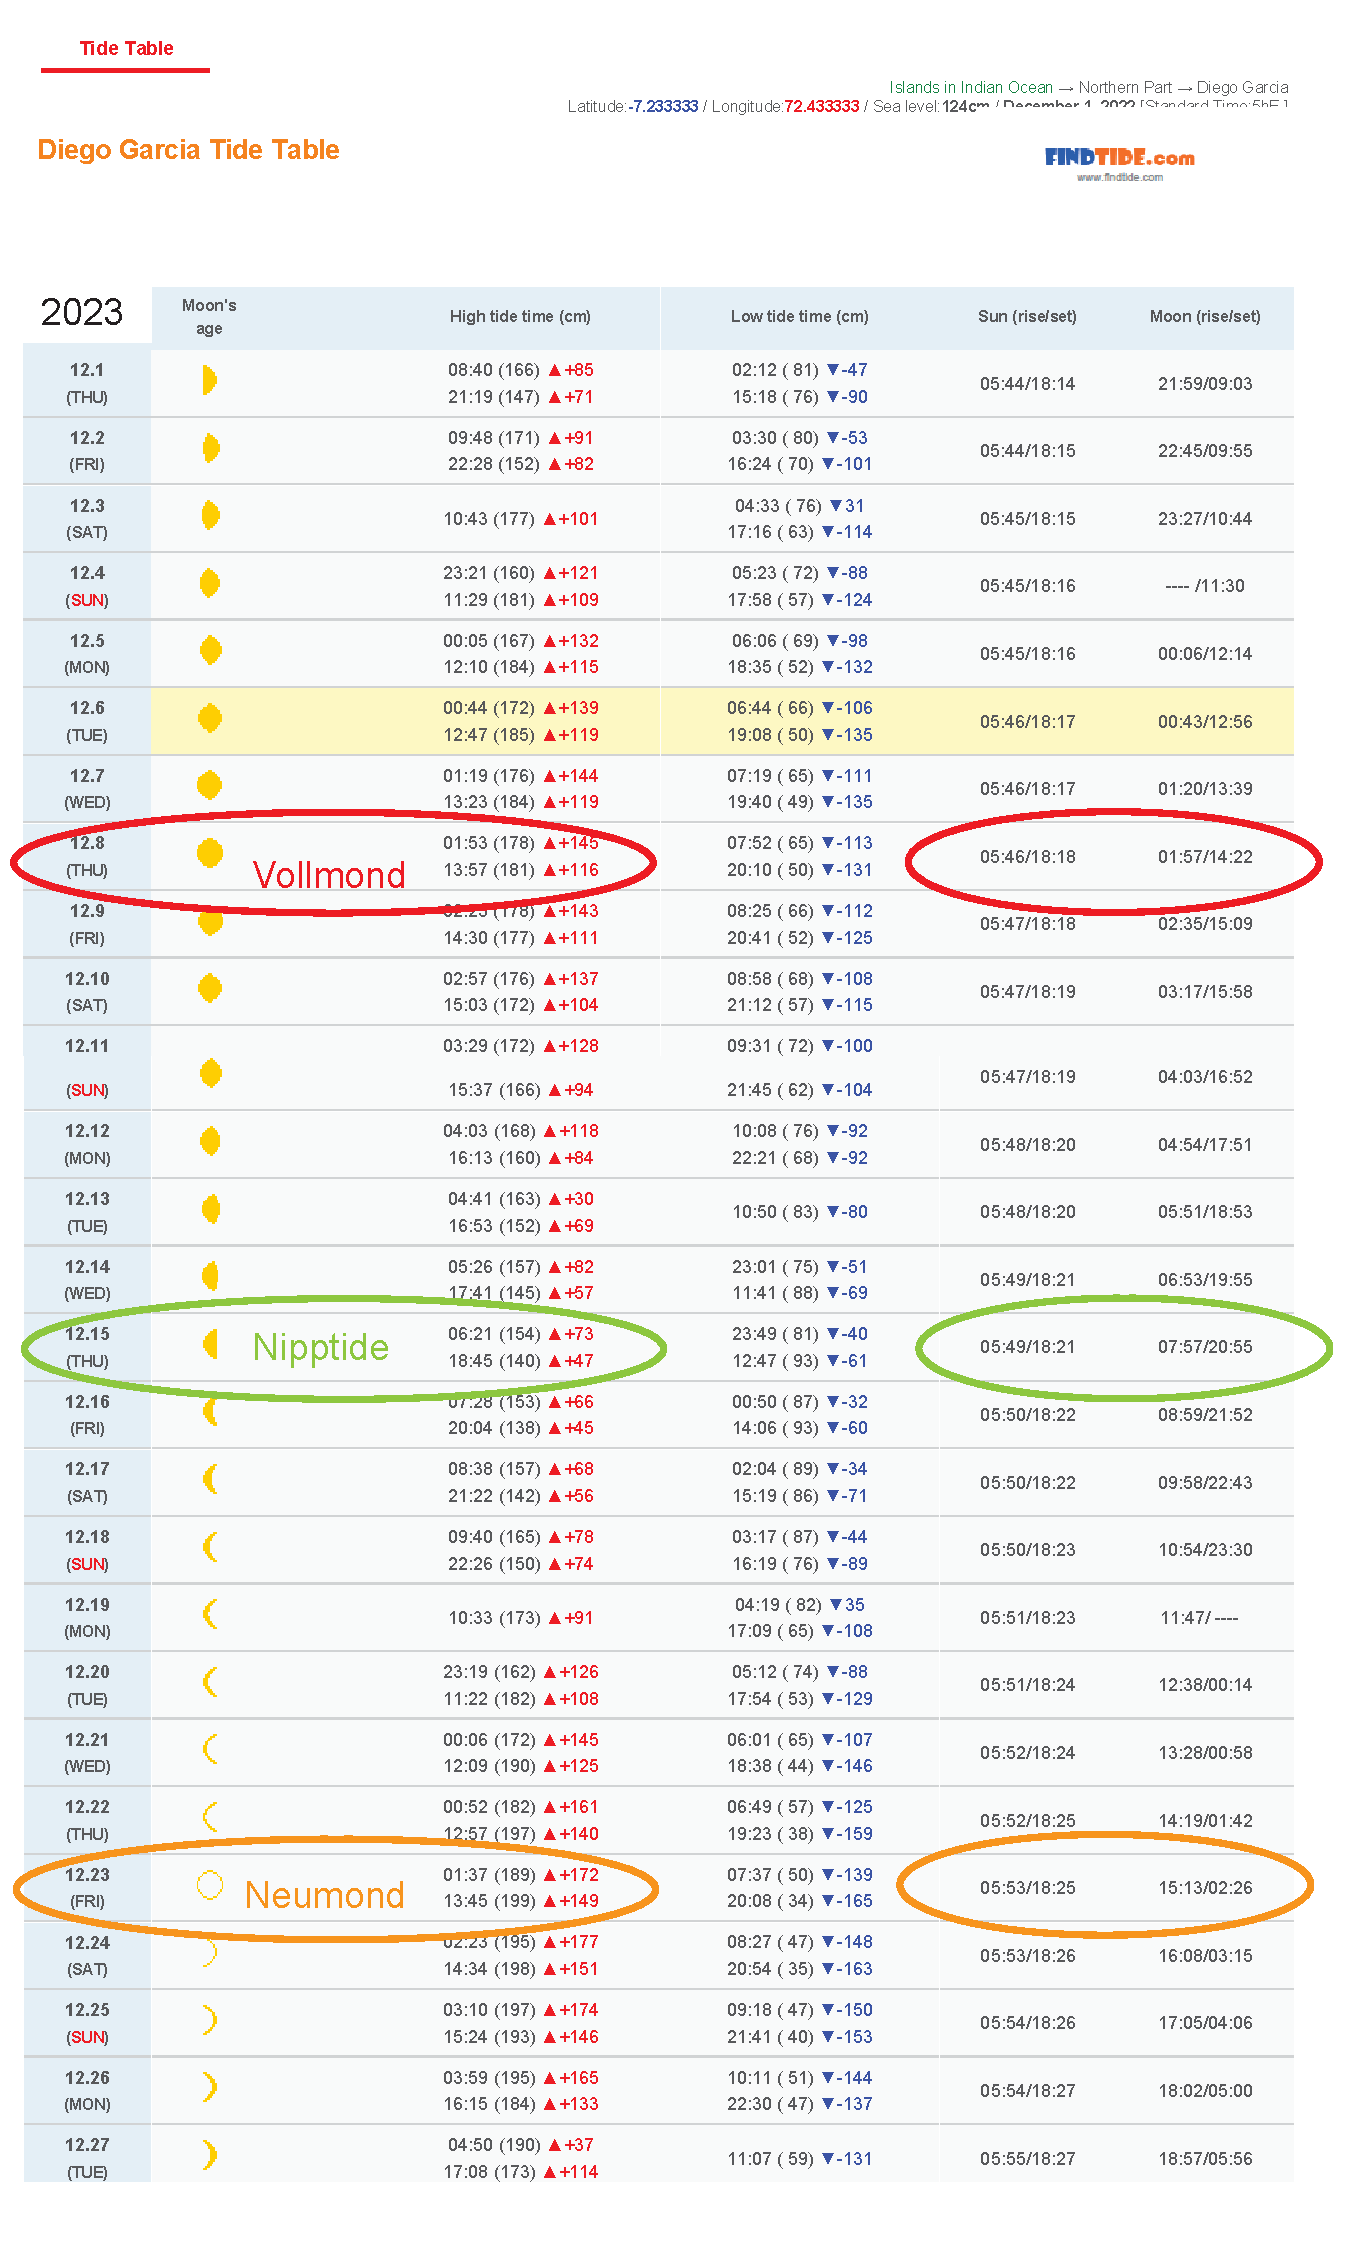
\includegraphics[width=\textwidth]{DiegoGarciaTideTableLsg.pdf}%
\caption{Tide Tabel von Diego Garcia im Indischen Ozean mit Beobachtungen}
	\label{abb:hm_DiegoGarciaTideTableLsg}
\end{figure}

\newpage

%-----------------------------------------------------------------------------------------------------------

\begin{sol} {prob:hm_gezeiten04} \label{lsg:hm_gezeiten04} %�bung36
\textbf{Gezeitenellipsoid}\\

\begin{itemize}
	\item \textit{\textbf{Newtonsche Gezeitentheorie}}\\ \\
	Wir verweisen auf \mlhmref{Gezeitenellipsoid.m}.

\begin{figure}[H]
	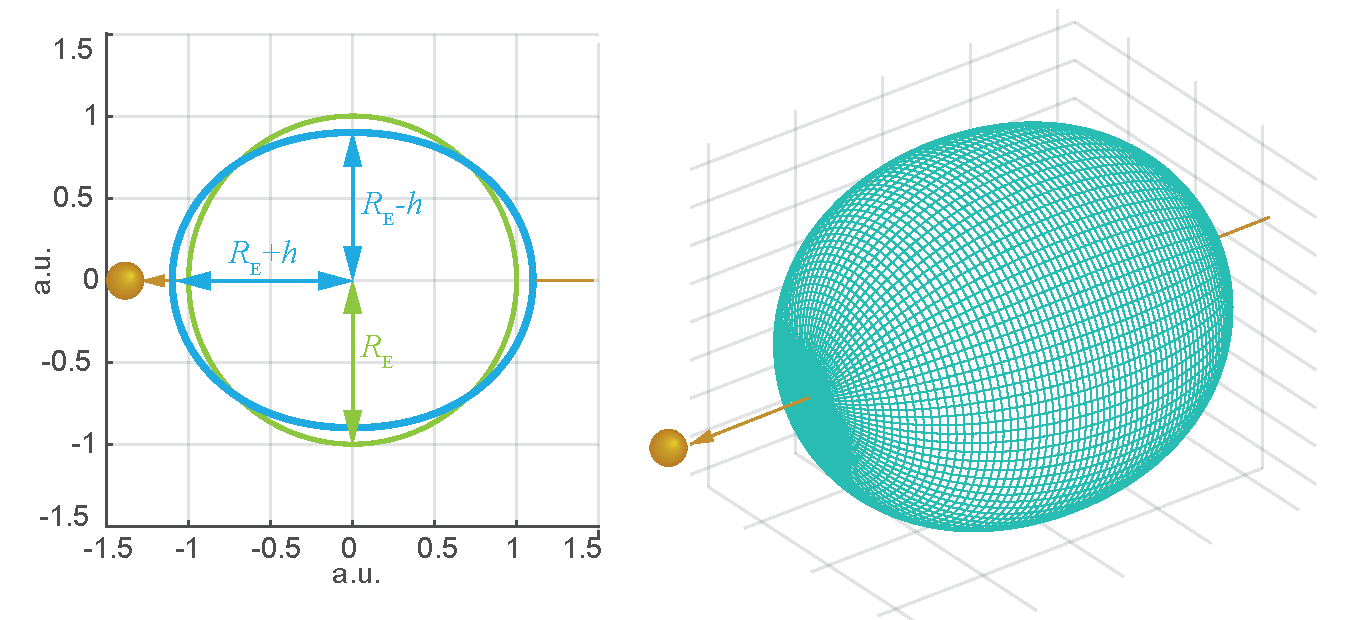
\includegraphics[width=\textwidth]{Gezeiten05.pdf} 
	\caption{Gezeitenellipsoid}
	\label{abb:hm_lsggezeiten04}
\end{figure}

F�r das Verh�ltnis der Volumina von Ellipsoid und Kugel finden wir :
	\[  \frac{V_\text{Ellip}}{V_\text{Kugel}} = \frac{(R_\text{E}+h)\,(R_\text{E}-h)^2}{R_\text{E}^3} \approx 1 - \frac{h}{R_\text{E}}  < 1\,,
	\]
was bedeutet, dass die angenommene Ellipsoidform nur eine N�herung sein kann. Eine verbesserte Rechnung m�sste sowohl die sogenannte Selbstgravitation des Gezeitenberges \cite{Norsen2017} als auch die Abflachungseffekte h�herer Ordnung sowie der bereits durch die Rotation der Erde hervorgerufene Abflachung \cite{Razmi2005} ber�cksichtigen.\\

	\item \textit{\textbf{Potentialtheorie}}\\ 

Wir benutzen \figref{hm_gezeiten02}. Das Potential der Gravitation des Mondes/der Sonne am Punkt $B$ ist gegeben durch: 
\begin{align*}
    U_\text{M} = -\frac{G\,m_\text{M}}{r'} ~~~~ \text{\bzw} ~~~~ U_\text{S} &= -\frac{G\,m_\text{S}}{r'}\,.
\end{align*}
Wir entwickeln $\vec{r}'= \vec{r} -\vec{R}$ wieder wie in \kap{hm_potentialtheorie} in sph�rischen Koordinaten $r,\theta$ (unter Ausnutzung der Rotationssymmetrie) und erhalten aus:
\begin{align}
    \frac{1}{r'} &= \frac{1}{\sqrt{r^2-2\vec{r}\,\vec{R} + R^2}} = \frac{1}{\sqrt{r^2-2r\,R\,\cos\theta+R^2}}  \label{eq:hm_lsggez31}\,.
\end{align}
Wir setzen jetzt $r= a_\text{EM}$ als festen Abstand der Mittelpunkte von der Erde und Mond und erhalten aus \eqref{eq:hm_lsggez31} wieder eine Entwicklung nach den Legendre-Polynomen analog zu \eqref{eq:hm_pot_theo07}
\begin{align}
    \frac{1}{r'} = \frac{1}{a_\text{EM}} \sum\limits_{n=0}^\infty \lk \frac{r}{a_\text{EM}}\rk^n\,\PL n\,\lk \cos\theta\rk\,. \label{eq:hm_lsggez32}
\end{align}
Daraus folgt mit $\mu_\text{M} = Gm_\text{M}$ das Potential am Punkt $B$ der Erdoberfl�che zu:
\begin{align}
    U_\text{M} = -\frac{\mu_\text{M}}{a_\text{EM}}\lek 1+\frac{r}{a_\text{EM}}\,\PL 1 \,\lk \cos\theta\rk + \frac{r^2}{{a_\text{EM}{}^2}}\,\PL 2 \,\lk\cos\theta\rk\rek\label{eq:hm_lsggez33}
\end{align}
und analog f�r die Sonne, wobei wir im Folgenden nun den Mond betrachten. \\
Der betrachtete Punkt $B$ erf�hrt im mitrotierenden Erde-Mond-System eine Zentrifugalkraft \bzw -Beschleunigung (siehe \probref{hm_gezeiten02})
\begin{align*}
    \vec{g}_\text{Z} &= -\omega_\text{M}{}^2\,\frac{m_\text{M}}{m_\text{M}+m_\text{E}} \,a_\text{EM}\,\vec{e}_\text{Z} \\
    &\approx -\omega_\text{M}\,\frac{m_\text{M}}{m_\text{E}}\,a_\text{EM}\,\vec{e}_\text{Z} = -\vec{\nabla}\,U_\text{Z}\,.
\end{align*}
Dies kann man mit \figref{hm_gezeiten02} als Potential
\begin{align}
    U_\text{Z} = \omega^2\,\frac{m_\text{M}}{m_\text{E}}\,a_\text{EM}\,r\,\cos\theta\label{eq:hm_lsggez34}
\end{align}
schreiben.\\
Wir benutzen, dass $\PL 1 \,\lk\cos\theta\rk = \cos\theta$ ist und erhalten mit $\omega^2 = \frac{\mu_\text{M}}{a_\text{EM}{}^3}$ (3. Keplersches Gesetz)
\begin{align}
    U_\text{Z} = \frac{\mu_\text{M}}{a_\text{EM}}\,\frac{r}{a_\text{EM}}\,\PL 1\,\lk\cos\theta\rk \label{eq:hm_lsggez35}\,.
\end{align}
Das gesamte auf den mitbewegten Punkt $B$ wirkende Potential ist dann die Summe von $U_\text{Z}$ und $U_\text{M}$, woraus folgt:
\begin{align}
    U = U_\text{Z} + U_\text{M} = -\frac{\mu_\text{M}}{a_\text{EM}}\,\lek 1+\frac{r^2}{a_\text{EM}{}^2}\,\PL 2\,\lk\cos\theta\rk\rek \,. \label{eq:hm_lsggez36}
\end{align}
Man erkennt aus \eqref{eq:hm_lsggez36}, dass sich die Terme, die linear in $r$ \bzw $\cos\theta$ sind, wegheben (bedingt durch die Balance von Gravitation und Zentrifugalkraft im rotierenden Erde-Mond-System) und dass als Zusatzterm zum Monopolpotential einer Punktmasse in 2. Ordnung das Gravitationspotential proportional zu $a_\text{EM}{}^{-3}$ �brig bleibt. \\ \\
Eine Fl�ssigkeit auf der Erdoberfl�che stellt sich in der H�he $h\lk\theta\rk$ und hat damit ein Potential $g\,h\lk\theta\rk$. Das gesamte Potential ist dann:
\begin{align}
    U_\text{total}\lk\theta\rk = -\frac{G\,m_\text{M}}{a_\text{EM}} + g\,h\lk\theta\rk- \zeta\,g\,\PL 2\,\lk\cos\theta\rk \label{eq:hm_lsggez37}
\end{align}
worin $\zeta$ durch
\begin{align*}
    \zeta = \frac{R_\text{E}{}^3}{a_\text{EM}{}^3}\,\frac{m_\text{M}}{m_\text{E}}\,R_\text{E}
\end{align*}
gegeben ist und wir $g= G\,m_\text{E}/r_\text{E}{}^2$ benutzt haben. \\
F�r eine Fl�ssigkeit muss das Potential $U$ unabh�ngig von $\theta$ sein, weil es sonst zu Ausgleichsstr�men kommt, womit sofort 
\begin{align}
    h\lk\theta\rk=\zeta\,\PL 2\,\lk\cos\theta\rk \label{eq:hm_lsggez38}
\end{align}
folgt und damit das bereits aus \eqref{eq:hm_gezeiten16} bekannte Ergebnis (bis auf konstante Terme).\\
In dieser Herleitung haben wir eine Fl�ssigkeit mit der Dichte $0$ unterstellt, die eine Erde die absolut fest ist komplett bedeckt. \\
Ein besseres Modell w�re sicher ein Zwei-Komponenten-Modell aus einem Planeten mit mittlerem Radius $R_\text{E}$, der einen homogenen inkompressiblen Ozean der Dichte $\rho_\text{W}$, einen homogenen, festen Kern der Dichte $\rho_\text{K}$ und eine Steifigkeit $\mu$ hat. Um dieses Modell zu berechnen, muss man die Effekte des Gravitationsfeldes des Gezeitenellipsoids selbst (die sogenannte Eigengravitation) und die der elastischen Kr�fte im Kern ber�cksichtigen. 
Wir verweisen %auf das erweiterte Problem in \probref{hm_gezeiten_zusatz} und 
die Spezialliteratur \cite{Murray2008,Norsen2017}.

\end{itemize}

\medskip \end{sol}
\textcolor{blue} {$\rightarrow$ zur} \probref{hm_gezeiten04}.\\
\noindent\rule[1ex]{\textwidth}{0.5pt} \newpage

%-----------------------------------------------------------------------------------------------------------

\begin{sol} {prob:hm_gezeiten05} \label{lsg:hm_gezeiten05} %�bung37
\textbf{Wasserkanal nach Airy \cite{Butikov2001}.}\\ \\

Einfaches Modell zur Dynamischen Theorie: 
Wir beziehen uns auf die instruktive Darstellung in \cite{Butikov2001}.
Wir betrachten den Airy-Wasserkanal entlang des �quators um die Erde und eine erzwungene Gezeitenschwingung (elliptischer Form) $q_1(t)$, deren Hauptachse auf die Erde-Mond-Linie ausgerichtet ist. Eine weitere Gezeitenschwingung (elliptischer Form), deren Hauptachse um $45\degree$ zur Erde-Mond-Linie verdreht ist, sei durch $q_2(t)$ gegeben. Die erzwungenen Wasserschwingungen im Kanal haben eine Eigenfrequenz $\omega_\text{Welle}$, die im Wesentlichen durch die Kanaltiefe bestimmt ist (siehe Band I) und die durch die halbt�gliche Gezeitenanregung mit $\omega_\text{Gez} = 2\,\omega_\text{E}$ erzwungen werden:
\begin{align*}
	\ddot{q}_1 +2\gamma\,\dot{q}_1 + \omega_\text{Welle}^2\,q_1 = A_1\,\omega_\text{Welle}^2\,\cos(\omega_\text{Gez}t) \,, \\
  \ddot{q}_2 +2\gamma\,\dot{q}_2 + \omega_\text{Welle}^2\,q_2 = A_2\,\omega_\text{Welle}^2\,\sin(\omega_\text{Gez}t)  \,.
\end{align*}
Hierin sind $\gamma$ die D�mpfungen und $A_, A_2 $ die Amplituden der Anregung der Gezeitenwellen.
Die Wasserh�hensteigung im Kanal an einer beliebigen Stelle des �quators (gegeben durch $R_\text{E},\, \theta$) ist dann gegeben durch:
	\[\Delta h = q_1\lk t\rk \cos 2\theta + q_2\lk t\rk \sin 2\theta \,.
	\]
F�r den Fall einer extrem langsam rotierenden Erde ist die Wasserh�hensteigung durch die station�re L�sung  $q_i(t)$ gegeben durch, wobei wir die Amplituden $A_1,\,A_2$ f�r beide Gezeitenwellen gleich annehmen wollen:
\begin{align}
   \Delta h &= q_1\lk t\rk \cos 2\theta + q_2\lk t\rk \sin 2\theta  \nonumber \\
    &= A\lek \cos\lk 2\omega_\text{Gez}t \rk \, \cos 2\theta + \sin \lk 2\omega_\text{Gez}t \rk \,\sin 2\theta \rek  \nonumber \\
    &= A\, \cos \lk 2\lk \omega_\text{Gez}t-\theta\rk\rk\,,  \label{eq:hm_gezeitenlsg01}
\end{align}
was bedeutet, dass die elliptischen Gezeitenverformungen der langsam rotierenden Erde folgen. Die Hauptachse der Gezeitenellipse ist immer auf die Erd-Mond-Linie ausgerichtet. \\
F�r beliebige $\omega_\text{E}$ benutzen wir als L�sung f�r die $q_i\lk t\rk$ die Berechnungen f�r den getriebenen Oszillator nach Gleichung (1.165) aus Kapitel 1.3.2 (Band I) mit der Amplitude
\begin{align*}
     \hat{q} &= \frac{\omega_\text{Gez}\,A}{\sqrt{\lk \omega_\text{Welle}{}^2\, - \,\omega_\text{Gez}{}^2\rk^2 + 4\gamma^2\,\omega_\text{Gez}{}^2}} \,,
\end{align*} 
und der Phase
\begin{align*}
    \delta &= \arctan\lek \frac{2\gamma\,\omega_\text{Gez}}{\omega_\text{Welle}{}^2 - \omega_\text{Gez}{}^2}\rek \,.
\end{align*} 
Daraus folgt nun f�r den Wasserh�henanstieg im Kanal:
\begin{align}
   \Delta h &= q_1\lk t\rk \cos 2\theta + q_2\lk t\rk \sin 2\theta  \nonumber \\
            &= \hat{q}\,\lek \cos\lk 2\omega_\text{E}t-\delta\rk\,\cos 2\theta + \sin\lk 2\omega_\text{E}t-\delta\rk\,\sin 2\theta\rek \nonumber \\
            &= \hat{q}\,\cos\lek 2\,\lk \omega_\text{E}t-\delta/2-\theta\rk\rek \,. \label{eq:hm_gezeitenlsg02}
\end{align}
Man erkennt aus \eqref{eq:hm_gezeitenlsg02}, dass der HW-Zeitpunkt an einer bestimmten Stelle des Erd�quators $R_\text{E},\, \theta$ gegeben ist durch:
\begin{align*}
    \theta_\text{max} = \omega_\text{E}\,t - \frac{\delta}{2}\,,
\end{align*}
was bedeutet, dass das Hochwasser mit einer bestimmten Zeitverschiebung  $\delta/2$ gegen�ber der Kulmination des Mond eintritt. Diese Verschiebung h�ngt von der Eigenfrequenz $\omega_\text{Welle}$ der Gezeitenwelle und ihrer D�mpfung $\gamma$ ab. In \figref{hm_lsggezeiten05} haben wir die �berlagerung und Verschiebung zur Erde Mond-Linie dargestellt.
Eine Simulation findet sich in \mlhmref{SimulationAiry.m}.

\begin{figure}[H]
	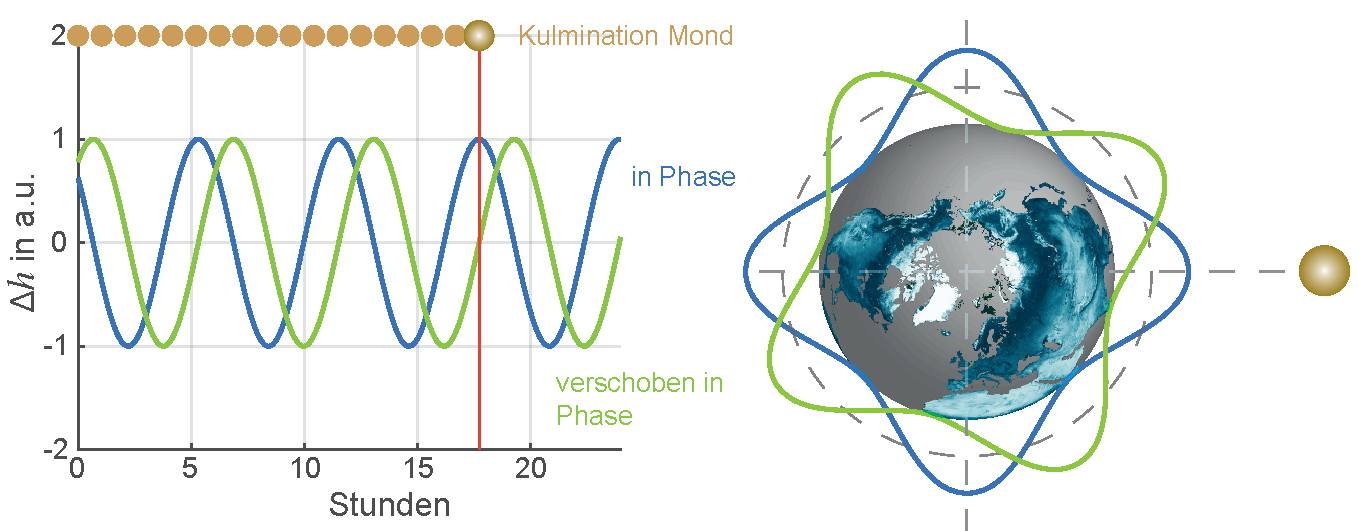
\includegraphics[width=\textwidth]{SimulationAiry.pdf} 
	\caption[Einfaches Modell zur Dynamischen Theorie.]{Einfaches Kanal-Modell nach Airy zur dynamischen Theorie der Gezeiten. Siehe auch \mlhmref{SimulationAiry.m}.
}
	\label{abb:hm_lsggezeiten05}
\end{figure}


\medskip \end{sol}
\textcolor{blue} {$\rightarrow$ zur} \probref{hm_gezeiten05}.\\
\noindent\rule[1ex]{\textwidth}{0.5pt} \newpage

%-----------------------------------------------------------------------------------------------------------

\begin{sol} {prob:hm_gezeiten06} \label{lsg:hm_gezeiten06} %�bung38
\textbf{Gezeitenreibung Hantelmodell}\\ \\

Die Rechnungen sind im Detail im \mscr{} \mlhmref{GezeitenReibung02.m} hinterlegt.
\begin{figure}[H]
	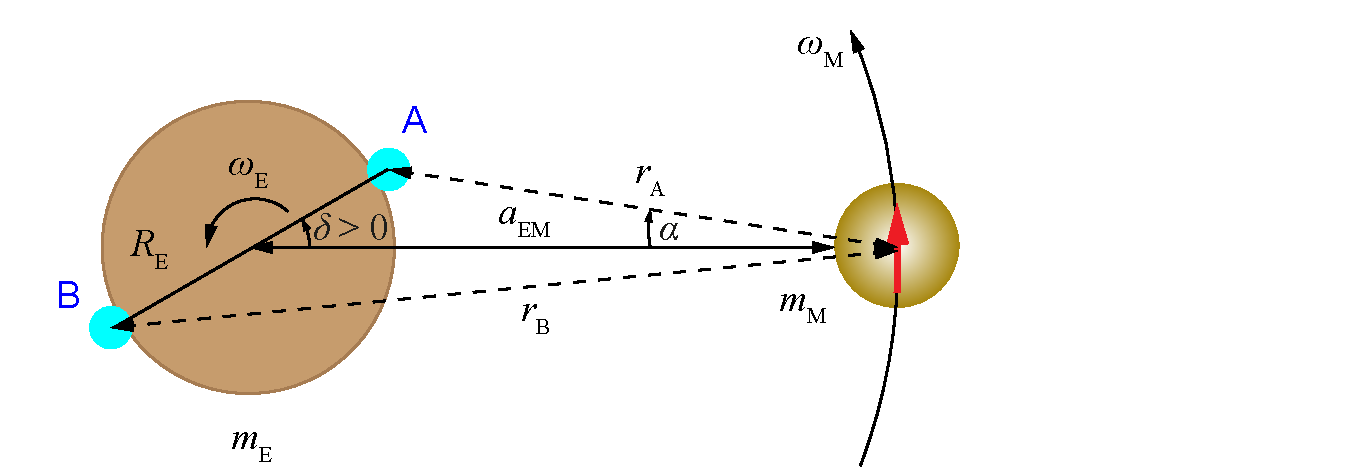
\includegraphics[width=\textwidth]{GezeitenHantel.pdf} 
	\caption{Gezeitenreibung - Hantelmodell}
	\label{abb:hm_lsggezeiten06}
\end{figure}
F�r die Berechnungen geben wir folgende Hinweise und Vorgehensweise zun�chst zur Ableitung des Drehmomentes aus \figref{hm_lsggezeiten06} an:
\begin{enumerate}
    \item [1)] Als erstes berechnen wir die Drehimpulse f�r den heutigen Zustand (Wir lassend dabei den Index 0 weg.):
    \begin{align*}
        L_\text{E} &= J_\text{E}\,\omega_\text{E}\,,~~ J_\text{E}\, \text{wird sp�ter berechnet}\,,~~~ \omega_\text{E} = \frac{2\pi}{\SI{86125}{\second}} \\
        L_\text{M} &= J_{\text{M}}\,\omega_\text{M} = m_\text{M}\,a_\text{EM}{}^2\,\omega_\text{M}\,, ~~~\omega_\text{M} = \frac{2\pi}{T_\text{synod.}}\,.
    \end{align*}
    %2)
    \item [2)] In der finalen Situation gilt: $\omega_\text{E,f} = \omega_\text{M,f}$:
    \begin{align*}
        L_\text{E,f} &= J_\text{E}\,\omega_\text{E,f}~,~~  L_\text{M,f} = J_\text{M,f}\,\omega_\text{M,f} = m_\text{M}\,a_\text{EM,f}{}^2\,\omega_\text{M,f}\,.
		\end{align*}
    %3)
    \item [3)] Aus der Drehimpulserhaltung folgt:
    \begin{align*}
        L_\text{ges} = J_\text{E}\,\omega_\text{E} + J_\text{M}\,\omega_\text{E} = J_\text{E}\,\omega_\text{E,f} + J_\text{M,f}\,\omega_\text{M,f}\,
    \end{align*}
und mit
    \begin{align*}
        \omega_\text{E,f} &= \omega_\text{M,f} ~~\rightarrow~~J_\text{E}\,\omega_\text{E} + J_\text{M}\,\omega_\text{M} = \lk J_\text{E} + J_\text{M,f}\rk\,\omega_\text{M,f}\,.
    \end{align*}
    Wir vergleichen:
    \begin{align*}
        J_\text{E} &\approx \frac{2}{5}\,m_\text{E}\,R_\text{E}{}^2\,~~\text{und}~~ J_\text{M,f} > J_\text{M} = m_\text{M}\,a_\text{EM}{}^2 ~\rightarrow~
        \frac{J_\text{E}}{J_\text{M}} = \frac{2}{5}\,\frac{m_\text{E}}{m_\text{M}}\,\frac{R_\text{E}{}^2}{a_\text{EM}{}^2} = 0.0045 \ll 1\,.
    \end{align*}
    Deswegen k�nnen wir in guter N�herung $J_\text{E} \ll J_\text{M,f}$ annehmen, womit folgt:
    \begin{align}
        L_\text{ges} = J_\text{E}\,\omega_{\text{E}} + J_\text{M}\,\omega_\text{E} = J_\text{M,f}\,\omega_\text{M,f} \label{eq:hm_gezUebg01} \,.
    \end{align}
    %4)
    \item[4)] Wir bestimmen nun den endg�ltigen Erde-Mond-Abstand $a_\text{EM,f}$ und die endg�ltige Kreisfrequenz $\omega_\text{M,f}$. Dazu betrachten wir die Kr�ftebilanz im finalen Zustand:
    \begin{align}
        \frac{G\,\killA{m_\text{M}}\,m_\text{E}}{a_\text{EM,f}{}^2} = \killA{m_\text{M}}\,\omega_\text{M,f}{}^2\,a_\text{EM,f} \label{eq:hm_gezUebg02} \,.
    \end{align}
    Aus \eqref{eq:hm_gezUebg01} und \eqref{eq:hm_gezUebg02} folgt
    \begin{align}
        a_\text{EM,f} &= \frac{L_\text{ges}{}^2}{G\,m_\text{E}\,m_\text{M}{}^2} \label{eq:hm_gezUebg03} \\
        \omega_\text{M,f} &= \frac{L_\text{ges}}{m_\text{M}\,a_\text{EM,f}{}^2} = \frac{G^2\,m_\text{E}{}^2\,m_\text{M}{}^3}{L_\text{ges}^3}\,. \label{eq:hm_gezUebg04}
    \end{align}
    %5)
    \item [5)] Zur Berechnung von $L_\text{ges}$ brauchen wir noch das Tr�gheitsmoment der Erde. \\
    Wir wollen die Erde aus einem Kern mit Dichte $\varrho_\text{K}$ und Radius $R_\text{K}$ und einer Schale $\varrho_\text{S}$ im Radiusbereich $R_\text{U}$ bis $R_\text{E}$ annehmen.
    \begin{align*}
        J_\text{E} &= \frac{2}{5}\,\lk \frac{4}{3}\,\pi\,\varrho_\text{S}\,R_\text{E}{}^3\rk\,R_\text{E}{}^2 + \frac{2}{5}\,\lk \frac{4}{5}\pi\,\lk \varrho_\text{K}-\varrho_\text{S}\rk\,R_\text{K}{}^3\rk\,R_\text{K}{}^2 \\
        &= \frac{2}{3}\,\frac{4}{3}\,\pi\lek \varrho_\text{S}\,R_\text{E}{}^5 + \varrho_\text{K}\,R_\text{K}{}^5 - \varrho_\text{S}\,R_\text{K}{}^5\rek = \frac{8}{15}\,\pi\lek \varrho_\text{S}\,\lk R_\text{E}{}^5 -R_\text{K}{}^5\rk + \varrho_\text{K}\,R_\text{K}{}^5\rek \\
        &\approx \SI{7.83e37}{\kg\square\metre}\\
        \text{\vgl homogene Erde} ~~~~ J_\text{EK} &= \frac{8}{15}\,\pi\,\varrho_\text{E}\,R_\text{E}{}^5 = \SI{9.7e37}{\kg\square\metre} \,.
    \end{align*}
    %6)
    \item[6)] Damit erhalten wir
    \begin{align*}
        L_\text{ges} &= J_\text{E}\,\omega_\text{E} + J_\text{M}\,\omega_\text{M} \approx \SI{3.45e34}{\kg\square\metre\per\second}\,.
    \end{align*}
    %7)
    \item[7)] Aus \eqref{eq:hm_gezUebg03} und \eqref{eq:hm_gezUebg04} erhalten wir:
    \begin{align*}
        a_\text{EM,f} &= \SI{5.55e8}{\km} = 1.44\,a_\text{EM}\,~~\text{und}~~ \omega_\text{M,f} = \SI{1.528e-6}{\per\second} ~~\rightarrow ~~T_\text{E,f} = \frac{2\pi}{\omega_\text{M,f}} = \SI{47.59}{}~\mathrm{d}\,.
    \end{align*}
    %8)
   \item [8)] Jetzt wollen wir noch wissen, wie lange es dauert bis der finale Zustand erreicht ist, \bzw um welche Distanz sich der Mond pro Jahrhundert entfernt. Nach \figref{hm_lsggezeiten06} ist:
    \begin{align*}
        F_\text{A} = \frac{G\,m\,m_\text{M}}{r_\text{A}{}^2} &= \frac{G\,m\,m_\text{M}}{a_\text{EM}{}^2 + R_\text{E}{}^2 - 2a_\text{EM}\,R_\text{E}\,\cos\delta} \\
        F_\text{B} = \frac{G\,m\,m_\text{M}}{r_\text{B}{}^2} &= \frac{G\,m\,m_\text{M}}{a_\text{EM}{}^2 + R_\text{E}{}^2 - 2a_\text{EM}\,R_\text{E}\,\cos\lk 180\degree-\delta\rk} \\
        &= \frac{G\,m\,m_\text{M}}{a_\text{EM}{}^2 + R_\text{E}{}^2 + 2a_\text{EM}\,R_\text{E}\,\cos\delta }
    \end{align*}
    Die Drehmomente auf die Hantel ergeben sich f�r kleine Winkel $\delta$ und $\alpha\approx 0$ zu:
    \begin{align*}
						\vec{M}_\text{D, A} &= \vec{R}_\text{E} \times \vec{F}_\text{A}\\
						M_\text{D, A}  &= R_\text{E}\,F_\text{A}\,\lk -\cos\delta\,\sin\alpha - \sin\delta\,\cos\alpha \rk \\
						\sin\delta &\approx \delta,~~\alpha \approx \frac{R_\text{E}}{r_\text{A}}\delta~\text{Sinussatz}\,~~~ \cos\alpha \approx 1,~~ \cos\delta \approx 1\,,\\
						M_\text{D, A}  &= +R_\text{E}\,F_\text{A}\,\delta \lk 1 + \frac{R_\text{E}}{r_\text{A}} \rk \,,~~
						M_\text{D, B}  = -R_\text{E}\,F_\text{B}\,\delta \lk 1 - \frac{R_\text{E}}{r_\text{A}} \rk \,, \\
						\rightarrow ~~M_\text{D, ges}&\approx -R_\text{E}\delta \lk F_\text{A} - F_\text{B} \rk \,.
			\end{align*}
    F�r das Gesamtdrehmoment auf die Hantel nehmen wir f�r $m$  \ca $\SI{e-8}{}$ $m_\text{E}$ an (wegen $g_\text{gez}|g_\text{E}$) also $m\approx\SI{3.8e-16}{\kg}$, $\delta = 3\degree$ 
    \begin{align*}
        \rightarrow ~~~~  M_\text{D, ges} &= \SI{-4.39e16}{\N\metre}
    \end{align*}
    %9)
    \item[9)] 
		Die Bewegungsgleichung f�r den starren K�rper ergibt:
    \begin{align*}
        -\frac{\D L}{\D t}\,M &=  M_\text{D, ges} = \frac{\D L_\text{E}}{\D t} = J_\text{E}\,\dot{\omega}_\text{E} = \frac{\D }{\D t}\,\lk m_\text{M}\,\omega_\text{M}\,a_\text{EM,f}{}^2\rk
    \end{align*}
    Aus der Drehimpulserhaltung folgt:
    \begin{align*}
				L &= \frac{2}{5}\,m_\text{E}\,R_\text{E}{}^2\,\omega_\text{E} + m_\text{M}\,a_\text{EM}{}^2\,\omega_\text{M} \\
				\frac{\D L}{\D t} = 0 &= \frac{2}{5}\,m_\text{E}\,R_\text{E}{}^2\,\dot{\omega}_\text{E} + 2m_\text{M}\,a_\text{EM}\,\dot{a}_\text{EM}\,\omega_\text{M} + m_\text{M}\,a_\text{EM}{}^2\,\dot{\omega}_\text{M} ~~~~ \Bigg|\substack{:\lk 2m_\text{M}\,a_\text{EM}{}^2\,\omega_\text{M} \rk}\\					0 &= \frac{1}{5}\,\frac{m_\text{E}\,R_\text{E}{}^2}{m_\text{M}\,a_\text{EM}{}^2}\,\frac{\dot{\omega}_\text{E}}{\omega_\text{M}} + \frac{\dot{a}_\text{EM}}{a_\text{EM}} + \frac{1}{2}\,\frac{\dot{\omega}_\text{M}}{\omega_\text{M}} \\
					\omega_\text{M} &= \sqrt{G\,m_\text{M}}\,a_{EM}{}^{-\frac{3}{2}} ~~~~ \rightarrow ~~~~ \dot{\omega}_\text{M} = \sqrt{G\,m_\text{M}}\,\lk -\frac{3}{2}\rk\,a_\text{EM}{}^{-\frac{5}{2}}\,\dot{a}_\text{EM} = -\frac{3}{2}\,\frac{\dot{a}_\text{EM}}{a_\text{EM}}\,\omega_\text{M} \\
				\rightarrow ~~~~ &-\frac{1}{5}\,\frac{m_\text{E}\,R_\text{E}{}^2}{m_\text{M}\,a_\text{EM}{}^2}\,\frac{\dot{\omega}_\text{E}}{\omega_\text{M}} = \frac{\dot{a}_\text{EM}}{a_\text{EM}}\,\lk 1-\frac{1}{2}\,\frac{3}{2}\rk \\
				\rightarrow ~~~~ &\frac{\dot{a}_\text{EM}}{a_\text{EM}} = -\frac{4}{5}\,\frac{m_\text{E}\,R_\text{E}{}^2}{m_\text{M}\,a_\text{EM}{}^2}\,\frac{\dot{\omega}_\text{E}}{\omega_\text{M}}\\
        \rightarrow ~~~~ &\dot{\omega_\text{E}} = \frac{M_\text{ges}}{J_\text{E}} \approx \SI{-5.61e-22}{\per\square\second} \,, \\
        \rightarrow ~~~~ &\dot{a}_\text{EM} = -2\,\frac{J_\text{E}\,\dot{\omega}_\text{E}}{m_\text{M}\,a_\text{EM}\,\omega_\text{M}} \approx \SI{1.17e-9}{\metre\per\second}\,.
    \end{align*}
    Umgerechnet bedeutet das f�r 100 Jahre:
    \begin{align*}
        \Delta T_\text{PE} &= -\frac{\dot{\omega}_\text{E}}{2\pi}\,T_\text{PE}{}^2\, \underbrace{100 \cdot 365 \cdot 86400}_{\substack{=100\,\mathrm{a}}} \SI{}{\second} = -\frac{\dot{\omega}_\text{E}}{\omega_\text{E}{}^2}\,2\pi\, 100\,\mathrm{a} \approx \SI{0.0021}{} \SI{}{\second} = \SI{2.1}{\metre\second}\,, \\
        \Delta a_\text{EM} &= \dot{a}_\text{EM}\, 100\,\mathrm{a} \approx \SI{3.7}{\metre}\,.
    \end{align*}
    %10)
\end{enumerate}

Jetzt wollen wir uns noch die Energiebilanz anschauen. Wir geben auch dazu die Vorgehensweise an:
    \begin{align*}
         E_\text{ges} &= \frac{J_\text{E}}{2}\,\omega_\text{E}{}^2 + \frac{J_\text{M}}{2}\,\omega_\text{M}{}^2 - \frac{G\,m_\text{M}\,m_\text{E}}{a_\text{EM}}\,,\\
         E_\text{ges} &= \frac{J_\text{E}}{2}\,\omega_\text{E}{}^2 + \frac{J_\text{M}}{2}\,\frac{G\,m_\text{E}}{a_\text{EM}{}^3} - \frac{G\,m_\text{M}\,m_\text{E}}{a_\text{EM}}\,, \\
        \rightarrow\frac{\D E}{\D t} &= J_\text{E}\,\omega_\text{E}\,\dot{\omega}_\text{E} - \frac{3}{2}\,\frac{J_\text{M}\,G\,m_\text{E}}{a_\text{EM}{}^4}\,\dot{a}_\text{EM} + \frac{G\,m_\text{E}\,m_\text{M}}{a_\text{EM}{}^2} \,\dot{a}_\text{EM} = P_\text{V} \approx \SI{-3.3e12}{\W}\,.
    \end{align*}
    Wir berechnen die \anf{Arbeit}, die die Gravitationsenergie beim Anheben der Ozeane leistet (pro Tag). Dazu brauchen wir zun�chst die Masse $m_\text{W}$ der angehobenen Wasserschicht:
    \begin{align*}
        m_\text{W} &= \frac{4}{3}\,\pi\,\lk R_\text{E} +h\rk^3\,\varrho - \frac{4}{3}\,\pi\,R_\text{E}\,\varrho = \frac{4}{3}\,\pi\,\varrho\,R_\text{E}{}^3\,\lk 1 + \frac{3h}{R_\text{E}} + \killA{\mathcal{O} \lk \frac{h^2}{R_\text{E}{}^2}\rk}\rk \,,\\
        \rightarrow ~ E_\text{W} &= -2m_\text{W}\,g\,h = \SI{-2.5e18}{\W} \,,\\
        P_\text{Diss} = \dot{E}_\text{Diss} &= -10\% \, \frac{E_\text{W}}{\SI{24}{\hour}} = \SI{-2.9e12}{\W} \,, \\
        E_\text{Diss} \lk 1a\rk &= P_\text{Diss} \, 1a = \SI{-25.4}{\peta\W\hour} = \SI{-25.4e4}{\tera\W\hour} \,.
    \end{align*}
    Wir vergleichen das mit dem weltweiten Prim�renergieverbrauch 2021 von 600 ExaJoule = $\SI{1.67e5}{\tera\W\hour}$, was bedeutet, dass die Gezeitenreibungs-Verlustenergie etwa $10\%$ des weltweiten Prim�renergieverbrauchs betr�gt. Wir k�nnen noch absch�tzen, zu welcher Erw�rmung der Ozeane das f�hrt, falls keine Abstrahlung ins Weltall erfolgen w�rde.
    \begin{align*}
        E_\text{Diss}\lk 1a\rk &= m_\text{W}\,c\,\Delta T~,~~~c_\text{W} = \SI{4.2}{}\,\frac{\SI{}{\kilo\J}}{\SI{}{\kg\K}}\,,\\
        \Delta T_\text{W} &= \frac{E_\text{Diss}\lk 1a\rk}{m_\text{W}\,c_\text{W}} \approx \SI{0.8}{\K} \,.
     \end{align*}

\medskip \end{sol}
\textcolor{blue} {$\rightarrow$ zur} \probref{hm_gezeiten06}.\\
\noindent\rule[1ex]{\textwidth}{0.5pt} \newpage

%-----------------------------------------------------------------------------------------------------------

\begin{sol}{prob:hm_gezeiten06a}\label{lsg:hm_gezeiten06a} %�bung39
\textbf{Gezeitenreibung - Auswirkung Mond.}\\ \\

Wir k�nnen die gleichen Gedankeng�nge wie im \kap{hm_gezeitenreibung} machen und erhalten die entsprechenden Gleichungen angepasst f�r den Mond.\\
Insbesondere ergibt \eqref{eq:hm_gezreibung08} nun:
\begin{align*}
    \frac{\dot{\Omega}_\text{M}}{\Omega_\text{M}} &= -\frac{45}{4}\,\frac{\omega_\text{M}{}^2}{\omega_\text{M}}\,\frac{m_\text{E}}{m_\text{M}}\,\lk \frac{R_\text{M}}{a_\text{EM}}\rk^3\,\frac{\delta}{1+\tilde{\mu}} \\
    &\approx \SI{1.1e-14}{\per\second}
\end{align*}
Die Zeitdauer, in der der Mond auf eine synchrone Eigenrotation gekommen ist, betr�gt dann
\begin{align*}
    \Delta T \approx \Big|\frac{\Omega_\text{M}}{\dot{\Omega}_\text{M}}\Big| \approx \SI{3e6}{} \text{Jahre}\,.
\end{align*}
Im Vergleich zum angenommenen Mondalter von ca. 4.5 Milliarden Jahren ist das eine verschwindend kurze Zeit. Daher ist es kaum �berraschend, dass der Mond schon lange eine synchrone Rotation zur Erde hat und uns immer das gleiche Gesicht zeigt.

\medskip \end{sol}
\textcolor{blue} {$\rightarrow$ zur} \probref{hm_gezeiten06}.\\
\noindent\rule[1ex]{\textwidth}{0.5pt} \newpage

%-----------------------------------------------------------------------------------------------------------

\begin{sol}{prob:hm_gezeiten07}\label{lsg:hm_gezeiten07} 
\textbf{Gravitationspotential au�erhalb eines Rotationsellipsoids.}\\ %�bung40

Wir nehmen die Form des homogenen Rotationsellipsoids mit
\begin{align}
    r'\lk \theta'\rk = R_0\lk 1-\frac{2}{3}\,\epsilon\,\PL 2\,\lk \cos\theta'\rk\rk \label{eq:hm_rotell01}
\end{align}
an, wobei $|\epsilon|\ll 1$ sein soll. \\
Nach \eqref{eq:hm_pot_theo07} in \kap{hm_pot_rotsymm_distrib} k�nnen wir das Potential an einem Ort $r,\, \theta$ vschreiben als:
\begin{align}
    U\lk r,\theta\rk = \sum_{n=0}^\infty \Phi_n\,\frac{\PL n \,\lk \cos\theta\rk}{r^{n+1}}\,, \label{eq:hm_rotell02}
\end{align}
worin
\begin{align}
    \Phi_n = -2\pi\,G\,\int\limits_0^\pi\int\limits_0^{r'\lk\theta'\rk}\,r'^{2+n}\,\varrho\lk r',\theta'\rk\,\PL n\lk\cos\theta'\rk \,\sin\theta'\,\D r'\,\D \theta'\,. \label{eq:hm_rotell03}
\end{align}
Das Integral ist �ber die gesamte Masseverteilung desK�rpers zu nehmen. \\
F�r einen homogenen K�rper der Dichte $\varrho$ k�nnen wir schreiben:
\begin{align}
    \Phi_n = -2\pi\,G\,\varrho\int\limits_0^\pi \PL n\,\lk\cos\theta'\rk \int\limits_0^{r'\lk \theta'\rk}r'^{2+n}\,\D r' \,\sin\theta'\,\D \theta'\,. \label{eq:hm_rotell04}
\end{align}
Die Integration �ber $r'$ ergibt:
\begin{align}
    \Phi_n = -\frac{2\pi\,G\,\varrho}{\lk n+3\rk}\int\limits_0^\pi \PL n\,\lk\cos\theta'\rk \,\lek r'\lk\theta'\rk\rek^{n+3}\,\sin\theta'\,\D \theta' \label{eq:hm_rotell05}\,,
\end{align}
in welches wir \eqref{eq:hm_rotell01} einsetzen und somit erhalten:
\begin{align}
    \Phi_n\approx -\frac{2\pi\,G\,\varrho}{\lk n+3\rk} \int\limits_0^\pi \PL n\,\lk \cos\theta'\rk R_0{}^{n+3}\,\lek \PL 0\lk\cos\theta'\rk - \frac{2}{3}\,\lk n+3\rk\,\epsilon\,\PL 2\lk\cos\theta'\rk\rek\,\sin\theta'\,\D \theta'\,. \label{eq:hm_rotell06}
\end{align}
Hier haben wir f�r $|\epsilon|\ll 1$\, $\lk 1+\epsilon\, x\rk^{n+3} \approx 1 + \lk n+3\rk\,\epsilon\, x$ und ferner $\PL 0\,\lk \cos\theta'\rk = 1$ benutzt.\\
Wegen der Orthogonalit�t der Legendre-Polynome (siehe \cite{Riley2006, Olver1992, Fischer2018} und die \onlineZ) k�nnen nur $\Phi_0$ und $\Phi_2$ von Null verschieden sein. Wir erhalten:
\begin{align}
\begin{split}
    \Phi_0 &= -\frac{4\pi\,G\,\varrho\,R_0{}^3}{3} = -G\,M\,, \\
    \Phi_2 &= \frac{8\pi\,G\,\varrho\,R_0{}^5\,\epsilon}{15} = \frac{2}{5}\,G\,M\,R_0{}^2\,\epsilon\,,
\end{split} \label{eq:hm_rotell07}
\end{align}
wobei wir mit $M = \frac{4\pi}{3}\,R_0{}^3\,\varrho$ die Masse der homogenen Kugel mit dem mittleren Radius $R_0$ bezeichnet haben.\\
Das Potential ergibt sich damit zu:
\begin{align*}
    U = U_0+U_2
\end{align*}
mit
\begin{subequations}
\begin{align}
      U_0 &= -\frac{G\,M}{r} \label{eq:hm_rotell08a} \,,\\
      U_2 &= \frac{2}{5}\,\frac{G\,M}{r^3}\,R_0{}^2\,\epsilon\,\PL 2\lk \cos\theta\rk \,.\label{eq:hm_rotell08b}
\end{align}
\end{subequations}
Man vergleiche diese Beziehung auch \eqref{eq:hm_rotell08b} mit dem Ansatz, welchen wir im Kapitel 1.5.5 im Band I f�r Herleitung der Frequenz der Pr�zessions der Erdachse im Gravitationsfeld des Mondes/der Sonne benutzt hatten.\\

\medskip \end{sol}
\textcolor{blue} {$\rightarrow$ zur} \probref{hm_gezeiten07}.\\
\noindent\rule[1ex]{\textwidth}{0.5pt} \newpage


%-----------------------------------------------------------------------------------------------------------

\begin{sol}{prob:hm_gezeiten09}\label{lsg:hm_gezeiten09} %�bung41
\textbf{Vergleich Gravitationseffekte auf die Erde}\\ \\

In \figref{hm_lsggezeiten10} und Tabelle \ref{tab:hm_Vergleich} haben wir die wesentlichen Charakteristika der Effekt zusammengefasst.

\begin{figure}[H]
	\includegraphics[width=\textwidth]{VergleichEffekte.pdf} 
	\caption{Vergleich verschiedener Effekte der Himmelsmechanik auf unsere Erde}
	\label{abb:hm_lsggezeiten10}
\end{figure}


\begin{sidewaystable}
\vspace{12cm}
\caption{Vergleich Gravitationseffekte auf die Erde} \label{tab:hm_Vergleich}
\begin{center}
\smallskip
%\begin{adjustbox}{width=\textwidth,totalheight=0.5\textheight,keepaspectratio}
\begin{tabular}{L{2.5 cm}L{2.5cm}L{2.6cm}L{5.5cm}L{4.5cm}}
\hline\noalign{\smallskip}
Effekt& KOS & Kr�fte \linebreak Drehmomente & Gr��enordnung Effekt & Charakteristische Werte \\
\noalign{\smallskip}\svhline\noalign{\smallskip}
Rotationsabplattung & Rotierendes System der Erde \linebreak Mitbewegter Beobachter & Zentrifugalkraft &$f = \frac{\omega_\text{E}{}^2\, R_\text{E}}{2\, g_\text{E}}$ & $f \approx 1:300$\linebreak $\Delta R \approx \SI{27}{\kilo\metre}$\\ \\ 
\hline\noalign{\smallskip}
Pr�zession der Erdachse & Inertialsystem & Drehmoment von Sonne und Mond wirkt auf Figurenachse des "`starren"' Erdk�rpers (Kreisel) &$\omega_\text{P} = -\frac{3G\,\cos\vartheta\,\Delta J }{2\, J_3\,\omega_\text{E}}\lk \frac{m_\text{S}}{{a_\text{ES}}^3}+\frac{m_\text{M}}{{a_\text{EM}}^3}\rk $ & $\omega_\text{P} = \SI{7.94e-12}{\per\second} \linebreak T_\text{P} = \frac{2\pi}{\omega_\text{P} } \approx 25\,100\,\text{Jahre} $ \\ \\
\hline\noalign{\smallskip}
Gezeiten& Inertialsystem & Gezeitenkraft von Mond und Sonne erzeugen auf fluider Oberfl�che Gezeitenellipse &$\frac{g_\text{Gez,M}}{g_\text{E}} = \frac{3}{2}\,\frac{m_\text{M}}{m_\text{E}}\,\frac{R_\text{E}{}^3}{r_\text{EM}{}^3} $ & $g_\text{Gez,M} \approx \SI{8.4e-8}{} g_\text{E} \linebreak g_\text{Gez,S} \approx \SI{3.9e-8}{} g_\text{E} \linebreak \Delta h_\text{M} \approx \SI{0.54}{\metre} \linebreak \Delta h_\text{S} \approx \SI{0.24}{\metre} $ \\ \\
\noalign{\smallskip}\hline\noalign{\smallskip}
Gezeitenreibung& Inertialsystem & Gezeitenkraft von Mond und Sonne erzeugt Drehmoment auf verdrehte Gezeitenellipse &$ M_\text{D}\approx \frac{9}{2}\,k\,\delta \,\frac{G\,m_\text{M}{}^2}{R_\text{E}}\,\lk \frac{R_\text{E}}{a_\text{EM}}\rk^6 $& $\Delta T_\text{PE}=-\frac{\dot{\omega}_\text{E}}{\omega_\text{E}}\,T_\text{PE}\,\,100\, \mathrm{a} \approx \SI{2.17e-03}{\second} \approx \SI{2.2}{\milli\second} $ pro Jh. \linebreak \linebreak$ \Delta a_\text{EM} \approx \SI{+4.7}{\metre}$ pro Jh. \\ \\
\noalign{\smallskip}\hline\noalign{\smallskip}
\end{tabular}
\end{center}
\end{sidewaystable}

\medskip \end{sol}
\textcolor{blue} {$\rightarrow$ zur} \probref{hm_gezeiten09}.\\
\noindent\rule[1ex]{\textwidth}{0.5pt}

\clearpage


%-----------------------------------------------------------------------------------------------------------
\newpage
%%%-----------------------------------------------------------------------------------------------------------
\subsection{�bungen zu Stabilit�t von Planetenbahnen, zur Periheldrehung des Merkurs und zu Sonnenfinsternissen}

\medskip

%-----------------------------------------------------------------------------------------------------------

\begin{sol}{prob:hm_hill_sphere} \label{lsg:hm_hill_sphere} %�bung42
\textbf{Warum hat der Mond keinen Mond?}\\ \\
So ganz stimmt die Frage nicht: Der Mond hat zumindest seit einigen Jahrzehnten k�nstliche Satelliten, die man als Monde des Mondes betrachten kann.
Wir wollen die Frage aber etwas generalisieren und betrachten dazu das in \figref{hm_Moon_of_Moon} dargestellte \anf{reduzierte} Dreik�rperproblem mit den Massen $m_1, m_2$ und einer kleineren Testmasse $m$.
Das Sonne ($m_\text{\astrosun}$) - Erde($m_\text{\earth}$) - Mond ($m_\text{M}$)-System kann man sich als einen speziellen Vertreter dieser Anordnung denken.
Die verallgemeinerte Fragestellung ist: Ab welchem Abstand $r_\text{H}$ bewegt die Masse $m$ nicht mehr auf einer geschlossenen Bahn um die Masse $m_2$.
Der Einfachheit halber nehmen wir kreisf�rmige Bahnen in einer Ebene an, so dass wir skalar rechnen k�nnen.

\begin{figure}[H]
	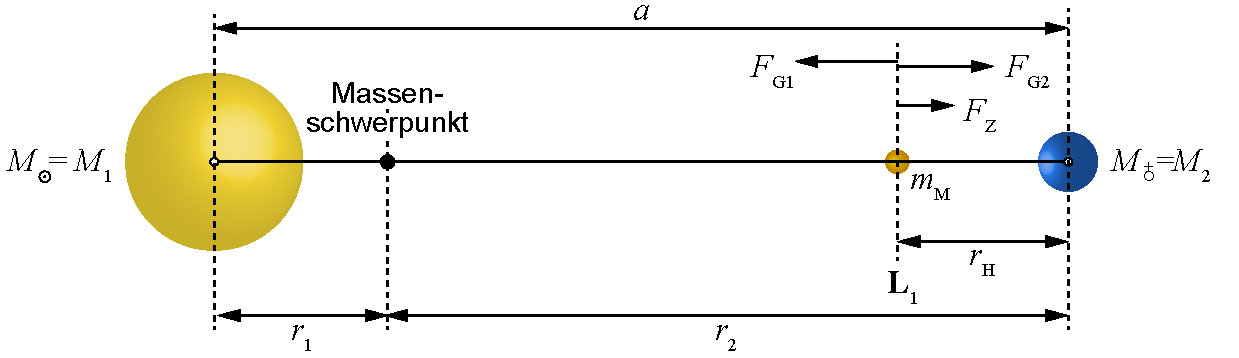
\includegraphics[width=0.8\textwidth]{Moon_of_Moon.pdf} 
	\caption[Zur Ableitung der Stabilit�tsbedingung.]{Zur Ableitung der Stabilit�tsbedingung (Hill Sph�re).}
	\label{abb:hm_Moon_of_Moon}
\end{figure}

Dann wollen wir uns einen ausgezeichneten Punkt zwischen den Massen $m_1$ und $m_2$ anschauen, an dem sich die Testmasse $m$ stabil aufhalten kann.
Dieser Punkt wird Lagrange-Punkt L$_1$ genannt.
Eine dort befindliche Testmasse $m$ rotiert um den Massenschwerpunkt des $m_1$-$m_2$-Systems mit der \emph{gleichen} Winkelgeschwindigkeit $\omega$ wie die Masse $m_2$.\footnote{Gewisserma�en \anf{geh�rt} die Testmasse an diesem Punkt weder zu $m_1$ noch zu $m_2$.
Es ist also der Grenzfall.} Wir erhalten aus der Geometrie der \figref{hm_Moon_of_Moon} die Abst�nde zum Massenschwerpunkt
\begin{align}
	r_1 &= \lk \frac{m_2}{m_1 + m_2} \rk a ~~\text{und} ~~~	r_2 = \lk \frac{m_1}{m_1 + m_2} \rk a ~.\label{eq:hm_moon_moon_lsg2}
\end{align}
Auf die Masse $m$ wirkt wegen ihrer kreisf�rmigen Bewegung um den Massenschwerpunkt die Zentrifugalkraft
\begin{equation}
F_z = m\omega^2 (r_2-r_\text{H}) ~~,\label{eq:hm_moon_moon_lsg3}
\end{equation}
worin wir $\omega$ durch das 3. Keplersche Gesetz ausdr�cken k�nnen:
\begin{equation}
\omega^2 = \frac{G(m_1+m_2)}{a^3}\label{eq:hm_moon_moon_lsg4} ~~.
\end{equation}
Es muss aber auch an dem Punkt L$_1$ die Zentrifugalkraft gleich den wirkenden Gravitationskr�ften der Massen $m_1$ und $m_2$ sein (damit ein Gleichgewicht herrscht), also
\begin{equation}
m\omega^2(r_2 - r_\text{H}) = \frac{Gmm_1}{(a-r_\text{H})^2} - \frac{Gmm_2}{r_\text{H}^2} ~~. \label{eq:hm_eq:moon_moon_lsg5}
\end{equation}
Wir setzen $\omega^2$ aus \eqref{eq:hm_moon_moon_lsg4} ein, dividieren durch $m$ und $G$ und erhalten
\begin{equation}
\frac{m_1+m_2}{a^3}(r_2-r_\text{H}) = \frac{m_1}{(a-r_\text{H})^2} - \frac{m_2}{r_\text{H}^2} ~~.\label{eq:hm_moon_moon_lsg6}
\end{equation}
Mit Substitution von $r_2$, $\gamma_\text{R}\!=\!m_2/m_1$ und $q\!=\!r_\text{H}/a$ erhalten wir aus \eqref{eq:hm_moon_moon_lsg6}
\begin{align}
	m_1 a- (m_1 + m_2) r_\text{H} &= \frac{m_1 a^3}{(a-r_\text{H})^2} - \frac{m_2 a^3}{r_\text{H}^2} ~~\Rightarrow~~a-(1+\gamma_\text{R})r_\text{H} = \frac{a^3}{(a-r_\text{H})^2} - \frac{\gamma_\text{R}a^3}{r_\text{H}^2} \nonumber\\
	\Rightarrow 1-(1+\gamma_\text{R})q &= \frac{1}{(1-q)^2} - \frac{\gamma_\text{R}}{q^2} ~~.\label{eq:hm_moon_moon_lsg7}
\end{align}
Diese Gleichung kann man nur numerisch l�sen, da sie ein Polynom 5. Grades in $q$ ist.
Umgeformt lautet sie
\begin{equation}
(1-q)^2 q^2 - (1+\gamma_\text{R})q^3 (1-q)^2 = q^2 - \gamma_\text{R}(1-q)^2 ~~.\label{eq:hm_moon_moon_lsg8}
\end{equation}
Wir k�nnen die Gleichung entweder numerisch l�sen und erhalten $q\!=\!r_\text{H}/a\!=\!f(\gamma_\text{R})$ (gute �bung in \matlab), oder wir machen eine sinnvolle N�herung, die z.\,B. f�r das Sonne-Erde-Mond-System gilt, mit 
\begin{align*}
	\gamma_\text{R} &= \frac{m_2}{m_1} \ll 1 ,\, q \ll 1 ~~~\Rightarrow 1+\gamma_\text{R} \approx 1 \;,~~(1-q)^2 \approx 1-2q \;~~\frac{1}{(1-q)^2} \approx= 1+2q ~~.
\end{align*}
Dann folgt aus \eqref{eq:hm_moon_moon_lsg7}
\begin{align*}
	1-q &= 1+2q - \frac{\gamma_\text{R}}{q^2} 	\Rightarrow q^2 - q^3 = q^2 + 2q^3 - \gamma_\text{R} ~~~	\Rightarrow ~~3q^3 = \gamma_\text{R} ~~
\end{align*}
und nach Resubstitution von $\gamma_\text{R}$ schlie�lich
\begin{equation}
r_\text{H} = a \sqrt[3]{\frac{m_2}{3 m_1}} ~~.\label{eq:hm_moon_moon_lsg9}
\end{equation}
Damit haben wir den maximalen Radius bestimmt, den ein Satellit mit Masse $m_2$ eines Planeten haben kann, bevor er vollst�ndig in das Gravitationsfeld des Zentralk�rpers mit Masse $m_1$ gelangt und selbst zum Kometen oder Planeten wird.
Dieser Radius wird zu Ehren von G. W. Hill\footnote{George William Hill (1838--1914) war ein US-amerikanischer Mathematiker und Astronom, der besonders auf dem Gebiet der theoretischen Astronomie zu Dreik�rperproblemen und der Mondtheorie forschte.} \emph{Hill-Radius} bzw. das entsprechende Volumen \emph{Hill-Sph�re} genannt.\\
Wir wollen zun�chst $r_\text{H}$ des Sonne-Erde-Mond-Systems berechnen.
Mit den Werten f�r $m_\text{\astrosun}\!=\!1.989\cdot 10^{30}\:$kg und $m_\text{\earth}\!=\!5.972\cdot 10^{24}\:$kg ergibt sich $r_\text{H,\earth}\!\approx\! 1.49\cdot 10^6\:$km.
Der Mond befindet sich mit einem Erdabstand von ca. $383000\:$km also gut innerhalb der Hill-Sph�re. \\
Wie sieht es nun aber beim Erde-Mond-\anf{Mond-Mond}-System aus?
Es folgt mit den Werten $m_\text{\earth}$ und $m_\text{M}\!=\!7.3\cdot 10^{22}\:$ kg ein Radius von $r_\text{H,M}\!\approx\! 61000\:$ km f�r die Hill-Sph�re.
Das ist etwas mehr als $1/7$ der Erde-Mond-Entfernung.
Es k�nnte also durchaus m�glich sein, dass der Mond selbst einen Begleiter hat (oder hatte).
Dass dies aber heute in der Realit�t nicht so ist, liegt an den starken Gezeitenkr�ften, die von Erde und Mond auf den Satelliten wirken und ihn mit der Zeit abbremsen w�rden (siehe \kap{adyn_forces}).
Nach einer gewissen Zeit in der Mondumlaufbahn w�rde die Testmasse (der Satellit) auf den Mond st�rzen. 
Es sei zum Schluss noch erw�hnt, dass die Formel f�r die Hill-Sph�re f�r elliptische Bahnen
\begin{equation}
r_\text{H} = (1-e)\,a\,\sqrt[3]{\frac{m_2}{3m_1}} \,. \label{eq:hm_hill_sphere_allg}
\end{equation}
lautet, was relativ einsichtig ist und im Detail in \cite{Murray2008} nachvollzogen werden kann.
\medskip \end{sol}
\textcolor{blue} {$\rightarrow$ zur} \probref{hm_hill_sphere}.\\
\noindent\rule[1ex]{\textwidth}{0.5pt} \newpage

%-----------------------------------------------------------------------------------------------------------

\begin{sol}{prob:hm_potential_merkur}\label{lsg:hm_potential_merkur} %�bung43
\textbf{Berechnung St�rpotential Merkur}\\
\begin{figure}[H]
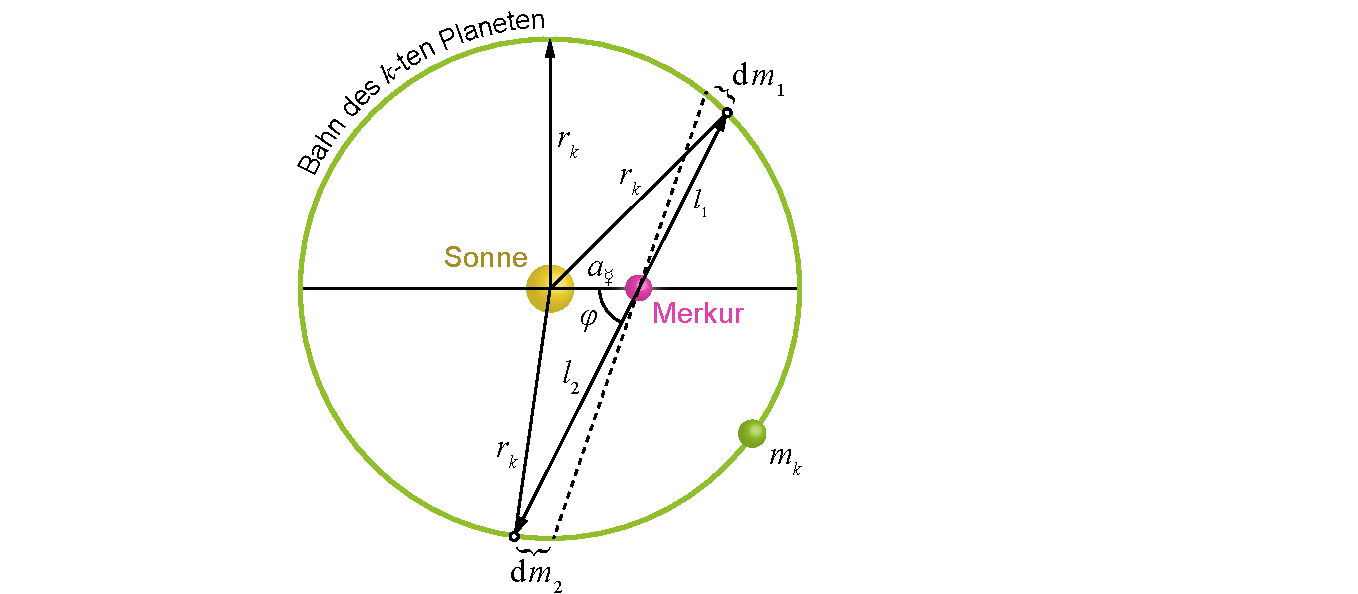
\includegraphics[width=\textwidth]{StoerpotentialMerkur_lsg}%
\caption[Geometrie zur Wirkung des St�rpotentials auf Merkur.]{Geometrie zur Wirkung des St�rpotentials einer Masse $m_k$ auf den Merkur.}%
\label{abb:hm_stoerpot_merkur_lsg}%
\end{figure}

Die Rechnungen sind im Detail im \mscr{} \mlhmref{StoerpotentialMerkur.m} ausgef�hrt. 
\begin{enumerate}[(a)]
	\item Wir benutzen die Geometrie der \figref{hm_stoerpot_merkur_lsg}.
          Der �u�ere Planet mit der Masse $m_k$ bewege sich gleichf�rmig auf der Kreisbahn mit $r_k$.
          Wir k�nnen dann seine Masse im Mittel \anf{verschmiert} auf den Ring mit dem Umfang $2\pi r_k$ verteilt annehmen.
          Die differentielle Massendichte auf der Umlaufbahn des $i$-ten Planeten mit dem Umfang $u_i$, die vom Merkur unter einem Winkel $\varphi$ gesehen wird, ist 
\begin{equation}
\D m_i = \lambda_k \,\D u_i = \frac{m_k}{2\pi r_k}\, l_i\,\D\varphi ~~. \label{eq:hm_pot_merk_lsg1}
\end{equation}
Die Newtonsche Gravitationskraft, die auf den Merkur wirkt, ist jeweils die Differenz der Massenwirkung $\D m_1$ und $\D m_2$, also
\begin{equation}
\D \vec{F} = m_\text{\mercury} G \lk \frac{\D m_1}{l_1^2} - \frac{\D m_2}{l_2^2} \rk \vec{l} ~~. \label{eq:hm_pot_merk_lsg2}
\end{equation}
Hierin ist $\vec{l}$ der Vektor, der vom Merkur zum differentiellen Massepunkt $\D m_1$ zeigt und, wie wir gleich sehen werden, eine Funktion des Winkels $\varphi$ ist.
Die Kraft, die in Richtung der Achse Sonne-Merkur wirkt (das ist die interessante Komponente, die ja das ZK-Feld der Sonne modifiziert), k�nnen wir schreiben als
\begin{equation*}
\D\vec{F}_{\text{SM}} = \D \vec{F}\,\cos\varphi ~~.
\end{equation*}
Wir k�nnen nun �ber $\D\vec{F}_{\text{SM}}$ integrieren und erhalten f�r den Beitrag des $k$-ten �u�eren Planeten �ber
\begin{equation*}
\D\vec{F}_{k,\text{SM}} = \vec{e}_{\text{\astrosun\mercury}}\,\int\limits_{-\pi/2}^{\pi/2} m_\text{\mercury} G \lambda_k \lk \frac{l_2 - l_1}{l_1 l_2} \rk \cos\varphi\,\D\varphi ~~.
\end{equation*}
Hierin haben wir mit $\vec{e}_{\text{\astrosun\mercury}}$ den Einheitsvektor in Richtung Sonne-Merkur bezeichnet.
Wir brauchen jetzt noch die $\varphi$-Abh�ngigkeit der L�ngen $l_1$ und $l_2$.
Mit dem Kosinussatz gilt
\begin{align*}
r_k^2 &= a^2 + l_1^2 - 2a l_1 \cos(\pi-\varphi) \\
\Rightarrow l_1 &= -a \cos\varphi + \sqrt{a^2\cos^2\varphi - \lk a^2-r_k^2 \rk}
\end{align*}
und
\begin{align*}
r_k^2 &= a^2 + l_2^2 - 2a l_2 \cos(\varphi) \\
\Rightarrow l_2 &= a \cos\varphi + \sqrt{a^2\cos^2\varphi - \lk a^2-r_k^2 \rk} ~~.
\end{align*}
Aus \eqref{eq:hm_pot_merk_lsg1} in \eqref{eq:hm_pot_merk_lsg2} eingesetzt erhalten wir
\begin{align*}
\D\vec{F}_{k,\text{SM}} &= m_\text{\mercury} G \lambda_k \lk \frac{l_1}{l_1^2} - \frac{l_2}{l_2^2} \rk \vec{l}\,\D\varphi \\
&= m_\text{\mercury} G \lambda_k \lk \frac{l_2 - l_1}{l_1 l_2} \rk \vec{l}\,\D\varphi ~~.
\end{align*}
Wir erkennen ferner aus der \figref{hm_stoerpot_merkur_lsg}, dass es zu den Kraftkomponenten, die senkrecht zu der Achse Sonne-Merkur wirken, jeweils eine positive und negative Komponente gibt.
Es verbleibt demnach als Netto-Effekt nur eine Komponente des Kraftvektors in Richtung Sonne-Merkur.
Wir machen weiter mit der hilfreichen Beziehung
\begin{align*}
\frac{l_2-l_1}{l_1 l_2} &= \frac{2a_\text{\mercury} \cos\varphi}{\killA{-a^2\cos^2\varphi} + \killA{a^2\cos^2\varphi} - (a^2_\text{\mercury} - r_k^2)} = \frac{2a_\text{\mercury} \cos\varphi}{r_k^2 - a_\text{\mercury}^2}
\end{align*}
und erhalten f�r die Gravitationskraft schlie�lich
\begin{align*}
F_k &= \frac{2 m_\text{\mercury} a_\text{\mercury} G}{r_k^2 - a_\text{\mercury}^2}\,\lambda_k \int\limits_{-\pi/2}^{\pi/2} \cos^2\varphi \, \D\varphi = \frac{\pi m_\text{\mercury} a_\text{\mercury} G \lambda_k}{r_k^2 - a_\text{\mercury}^2} ~~.         
\end{align*}
Die Wirkung des �u�eren Planeten ist also eine zentrale von der Sonne wegziehende Kraft (was nicht ganz �berraschend ist).
Grundlage f�r dieses Ergebnis waren folgende Annahmen:
\begin{itemize}
	\item Konzentrische Kreisbahnen der �u�eren Planeten und des Merkurs um die Sonne
	\item Wirkung des �u�eren Planeten auf den Merkur sind sehr klein
\end{itemize}

\item Wir berechnen die Frequenz $\omega\!=\!\sqrt{(-3/a) b(a)\!-\! b'(a)}\!\equiv\!\sqrt{\beta}$ nach \eqref{eq:hm_lsg_Stoer}.
  Stabile Bahnen gibt es, wenn der Ausdruck $\beta$ unter der Wurzel $>\!0$ ist.
  Wir berechnen die Beschleunigungen aus
\begin{align*}
b(r) &= -\frac{\d}{\d r}\,U(r) ~~\; \text{und} ~~\; b'(r) = -\frac{\d^2}{\d r^2}\,U(r) ~~.
\end{align*}
\begin{itemize}
	\item F�r den Fall $U(r)\!=\!-r^q$ ergibt sich 
	\begin{align*}
		b(r) &= +q r^q ~\;\text{und} ~\;	b'(r)= q(q-1)r^{q-1} ~~.
	\end{align*}
Mit $r\!=\!q\!=\!1$ folgt 
  \begin{align*}
		\beta &= -3q-q(q-1) > 0 ~~, \\
		\beta &= q(q+2) < 0 ~~.
	\end{align*}
Damit ist der stabile Bereich gegeben durch $-2\!<\!q\!<\!0$.
\smallskip
	\item F�r den Fall $U(r)\!=\! -1/r + C/r^3$ ergibt sich 
 	\begin{align*}
		b(r) &= -\frac{1}{r^2} + \frac{3C}{r^4} ~\;\text{und} ~\;	b'(r) = +\frac{2}{r^3} - \frac{12C}{r^5} ~~.
	\end{align*}
Mit $r\!=\!q\!=\!1$ folgt 
   \begin{align*}
		\beta &= -3(-1+3C)-2-12C >0 ~~, \\
		\beta &= 1+3C >0 ~~.
	\end{align*}
Damit ist der stabile Bereich gegeben durch $C\!>\! -1/3$.
\smallskip
\end{itemize}
\end{enumerate}
\medskip \end{sol}
\textcolor{blue} {$\rightarrow$ zur} \probref{hm_potential_merkur}.\\
\noindent\rule[1ex]{\textwidth}{0.5pt} \newpage


%-----------------------------------------------------------------------------------------------------------

\begin{sol}{prob:hm_perihel_kappa3}\label{lsg:hm_perihel_kappa3} %�bung44
\textbf{L�sung der Bewegungsgleichung und Periheldrehung bei einem $\kappa_3/r^3$ St�rpotential und Berechnung der relativistischen Perihelverschiebung des Merkurs}\\ \\
Wir setzen zun�chst in Gleichung \eqref{eq:hm_allg_ZK_1} $\kappa_2\!=\!0$.
Das ergibt
\begin{align}
\D \upsilon &= -\frac{\D q}{\sqrt{\frac{2H_g}{L^2} + \frac{2\mu_\text{G}}{L^2} q - \lk 1 - \frac{2\kappa_3 }{L^2} q \rk q^2 }} \nonumber \\
&= -\frac{\D q}{\sqrt{\hat{A}+ \hat{B} q + \hat{C} q^2 + \hat{D} q^3 }} ~~, \label{eq:hm_perihel_lsg_1} 
\end{align}
mit den Abk�rzungen
\begin{align*}
	\hat{A} = \frac{2H}{L^2} < 0 ~, \: \hat{B} = \frac{2\mu_\text{G}}{L^2} > 0 ~,\:	\hat{C} = -1 < 0 ~\; \text{und} ~\;\hat{D} = \frac{2\kappa_3}{L^2}~~.
\end{align*}
Dieses Integral ist nicht analytisch l�sbar.
Allenfalls kann man eine Reihenentwicklung machen.
Wir verfolgen hier einen st�rungstheoretischen Ansatz \cite{Greiner2003, Stephani1991}.
Dazu schreiben wir wieder die Radialbeschleunigung \eqref{eq:hm_beschl_polar} in Polarkoordinaten:
\begin{equation}
b(r) = b \lk \frac{1}{q} \rk = \lk \ddot{r} - r\dot{\upsilon}^2 \rk = -\frac{\d}{\d r}U(r) ~~.\label{eq:hm_perihel_lsg_2}
\end{equation}
F�r $\dot{r}$ gilt:
\begin{equation*}
\dot{r} = \frac{\D r}{\D \upsilon}\,\dot{\upsilon} = -\frac{1}{\killA{q^2}} \frac{\D q}{\D \upsilon} L \killA{q^2} = -L\,\frac{\D q}{\D \upsilon}~~
\end{equation*}
und analog f�r $\ddot{r}$: 
\begin{align*}
	\ddot{r} = \frac{\D}{\D t}\dot{r} &= -L \, \frac{\D}{\D t} \lk \frac{\D q}{\D \upsilon} \rk = -L \frac{\D }{\D \upsilon}\frac{\D \upsilon}{\D t} \lk \frac{\D q}{\D \upsilon} \rk = -L^2 q^2\,\frac{\D^2 q}{\D \upsilon^2}~~.
\end{align*}
Wir setzen beide Beziehungen in \eqref{eq:hm_perihel_lsg_2} ein und bekommen
\begin{align}
	-L^2 q^2 \,\frac{\D^2 q}{\D \upsilon^2} - \frac{1}{q}\,L^2 q^4 &= -\frac{\d}{\d r}U(r) = -\frac{\mu_\text{G}}{r^2} + \frac{3\kappa_3}{r^4}\nonumber\\
\Rightarrow \frac{\D^2 q}{\D \upsilon^2} + q &= \frac{1}{L^2 q^2}\,\frac{\d}{\d r}U(r) ~\nonumber\\
&= \frac{\mu_\text{G}}{L^2} - \frac{3\kappa_3}{L^2} q^2 ~. \label{eq:hm_perihel_lsg_3} 
 \end{align}
F�r $\kappa_3\!=\!0$ ergibt sich die bemerkenswert einfache Differentialgleichung 
\begin{equation}
\frac{\D^2 q}{\D \upsilon^2} + q = \frac{\mu_\text{G}}{L^2} \label{eq:hm_perihel_lsg_4} ~~, 
\end{equation}
aus deren L�sung sich sehr einfach die Bahnform bestimmen l�sst.
Denn es ist 
\begin{equation}
q(\upsilon) = \frac{\mu_\text{G}}{L^2} + A \cos\upsilon+ B\sin\upsilon \label{eq:hm_perihel_lsg_5} ~~,
\end{equation}
woraus man mit $q\!=\!1/r$ und $A\cos\upsilon + B\sin\upsilon\!=\! C\cos(\upsilon-\upsilon_0)$ nicht �berraschend die bekannte Kegelschnittgleichung \eqref{eq:hm_kegelschnitt} des Keplerproblems erh�lt.\footnote{Ohne Beschr�nkung der Allgemeinheit kann man $\upsilon_0\!=\!0$ setzen.} Wir erweitern nun \eqref{eq:hm_perihel_lsg_5} um $-3\kappa_3 q^2$ und schreiben f�r $\D^2 q / \D \upsilon^2 \!=\! q''$, so dass aus \eqref{eq:hm_perihel_lsg_3} folgt
\begin{align}
	q'' + q &= \frac{\mu_\text{G}}{L^2} - \frac{3\kappa_3 q^2}{L^2} \label{eq:hm_perihel_lsg_6}\\
	&\equiv A + \frac{B}{A}\,q^2 ~~, \nonumber
\end{align}
wobei $A\!=\!\mu_\text{G}/L^2 = 1/p$, $B/A\!=\!-3\kappa_3/L^2$ und $B\!=\!-3\kappa_3\mu_\text{G}/L^4$ gesetzt wurde.
Da $\kappa_3$ und daher $B/A$ kleine Gr��en sind, k�nnen wir f�r die L�sung dieser inhomogenen Differentialgleichung folgenden Ansatz machen:
\begin{align}
q &\approx q_K + B\:\hat{q} ~\label{eq:hm_perihel_lsg_7}\\
\Rightarrow q''_K + q_K + B \hat{q}'' + B\hat{q} &= A + \frac{B}{A} \lk q^2_K + 2 B\! q_K \!\hat{q} + B^2 \hat{q}^2 \rk ~~,
\end{align}
worin $q_K$ die Keplerl�sung f�r $\kappa_3\!=\!0$ ist.
Wir sortieren nach Potenzen von $B$ und bis zur Ordnung mit $B^1$.
Damit ergibt sich
\begin{align}
B^0 : ~ &q''_K + q_K = A ~~. \label{eq:hm_perihel_lsg_8a} \\ 
B^1 : ~ &\hat{q}'' + \hat{q} = \frac{1}{A} \lk q_K^2 + 2B \!q_K \hat{q}\rk = \frac{q_K}{A} \lk q_K + 2\hat{q} B \rk ~~\Rightarrow ~~\hat{q}'' + \hat{q} \lk 1 - \frac{2 B q_K}{A} \rk \approx \frac{q_K^2}{A}~~.  \label{eq:hm_perihel_lsg_8b}
\end{align}
Gleichung \eqref{eq:hm_perihel_lsg_8a} ist wie erwartet die bekannte Kepler-L�sung.
Wir setzen jetzt in \eqref{eq:hm_perihel_lsg_8b} f�r $q_K$ die Bahngleichung in der Form \eqref{eq:hm_kegelschnitt} ein und erhalten mit $q_K(\upsilon) = 1/p (1 + e\cos\upsilon) = A (1 + e\cos\upsilon) $ und $(A=1/p)$
\begin{align*}
	\hat{q}'' + \hat{q} &= p \lek \frac{1}{p} \lk 1+e\cos\upsilon\rk\rek^2 = \frac{1}{p} \lk  1+2e\cos\upsilon + \underbrace{e^2\cos^2\upsilon}_{= \frac{e^2}{2}(1+\cos 2\upsilon)}\rk \\
											&= \frac{1}{p} \lk  1+\frac{e^2}{2}+ 2e\cos\upsilon + \frac{e^2}{2}\cos 2\upsilon \rk~~.
\end{align*}
Da wir an Irregularit�ten der Bahn interessiert sind, schreiben wir die gesuchte Gesamtl�sung als lineare Superposition  $\hat{q}\!=\!\hat{q}_1 + \hat{q}_2 + \hat{q}_3$ und sortieren die einzelnen Elemente nach Vielfachen von $\upsilon$ im Argument des Kosinus:  
\begin{align}
\begin{split}
	\cos(0\upsilon): ~~ \hat{q}''_1 + \hat{q}_1 &= \frac{1}{p} \lk 1+\frac{e^2}{2}\rk~~, \\
	\cos(1\upsilon): ~~ \hat{q}''_2 + \hat{q}_2 &= 2\frac{e}{p} \cos\upsilon ~~, \\
	\cos(2\upsilon): ~~ \hat{q}''_3 + \hat{q}_3 &= \frac{e^2}{2p} \cos 2\upsilon ~~.
\end{split} \label{eq:hm_perihel_lsg_09a}
\end{align}
Die Einzell�sungen $\hat{q}_i$ der linearen Superposition sind (wie man leicht durch Differenzieren verifiziert):
\begin{align}
\begin{split}
\hat{q}_1 &= \frac{1}{p} \lk 1+\frac{e^2}{2}\rk ~~, \\
\hat{q}_2 &= \frac{e}{p}\,\upsilon \sin\upsilon ~~,\\ 
\hat{q}_3 &= -\frac{e^2}{6p}\,\cos 2\upsilon ~~.
\end{split} \label{eq:hm_perihel_lsg_09b}
\end{align}
Der eigentlich interessante Term ist der f�r $\hat{q}_2$.
Man erkennt an dieser Stelle, dass die Periheldrehung durch den nichtlinearen St�ranteil, der in der \eqref{eq:hm_perihel_lsg_3} vorhanden ist, hervorgerufen wird.
Die Gleichung f�r die gest�rte Bahn k�nnen wir schreiben als Keplerbahn plus St�rung $\hat{q}$:
\begin{equation}
q(\upsilon) = q_K + B \hat{q} = \frac{1+e\cos\upsilon}{p} + B (\hat{q}_1 + \hat{q}_2 + \hat{q}_3)~~. \label{eq:hm_perihel_lsg_9}
\end{equation}
Wir wollen jetzt analysieren, wie diese einzelnen St�rungen wirken.
Dazu fahren wir fort mit
\begin{equation}
pq(\upsilon) = 1 + \underbrace{e\cos\upsilon + Be\upsilon\sin\upsilon}_{\text{Term P}} + 1 + B \lek \lk 1+\frac{e^2}{2}\rk - \frac{e^2}{6} \cos{2\upsilon} \rek ~~, \label{eq:hm_perihel_lsg_10}
\end{equation}
wobei nur Term P zur Modifikation der Keplerbahn in Form einer Perihelverschiebung beitragen kann.
Wir k�nnen jetzt mit den Winkelfunktionen und unter Beachtung von $B \ll 1$ folgende Beziehung nutzen:
\begin{align*}
e\cos(\upsilon-B\upsilon)	&= e\cos\upsilon\,\underbrace{\cos(B\upsilon)}_{\approx 1} + e\sin\upsilon\,\underbrace{\sin(B\upsilon)}_{B\upsilon} = e\cos\upsilon + (Be\upsilon)\,\sin\upsilon\,
\end{align*}
Damit vereinfacht sich \eqref{eq:hm_perihel_lsg_10} zu
\begin{align*}
p\,q(\upsilon) &= 1 + \underbrace{e\cos(\upsilon-B\upsilon)}_{\text{Term I}} + B \underbrace{\lk a+\frac{e^2}{2} - \frac{e^2}{6}\,\cos 2\upsilon\rk}_{\text{Term II}}~~,
\end{align*}
wobei Term I \emph{nicht-periodisch} in $2\pi$ ist (und damit zu einer Periheldrehung f�hrt) w�hrend Term II periodisch in $2\pi$ (und damit nur f�r eine Oszillation des Radius verantwortlich ist).
Wir erhalten schlie�lich 
\begin{align}
r(\upsilon)	 &= \frac{p}{1+e\cos(\upsilon-B\upsilon)} \lk 1+ \frac{B C p}{1+e\cos{(\upsilon-B\upsilon)}} \rk^{-1} ~~. \label{eq:hm_perihel_lsg_11}
\end{align}
Damit haben wir eine n�herungsweise Beschreibung der Bahn f�r den gest�rten Fall mit $\kappa_3 \neq 0$ gewonnen.
\begin{figure}[H]
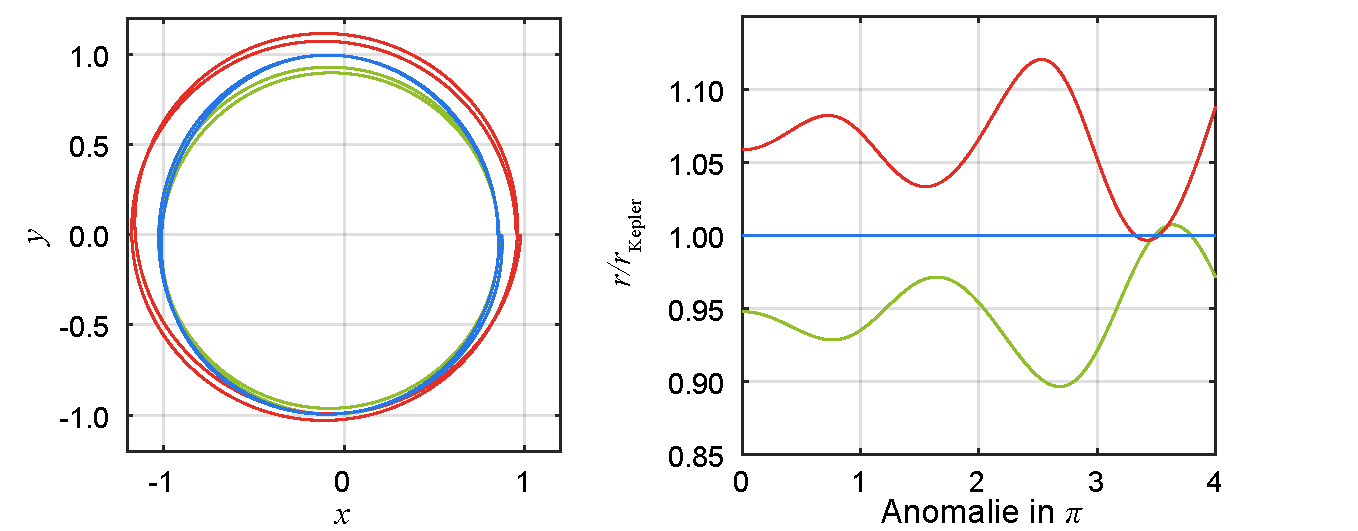
\includegraphics[width=\textwidth]{simulation_merkur2.pdf}%
\caption[Bahnkurven und Bahn-Oszillationen im Fall eines St�rpotentials.]{Bahnkurven und Bahn-Oszillationen im Fall eines St�rpotentials mit $\kappa_3 /{r^3}$\\ Parameter: $a=1, e = 0.1, \kappa_3 = + 0.02\,\mu_\text{G}/a^2 >0 $ (rot) und $\kappa_3-0.02\,\mu_\text{G}/a^2 < 0$ (gr�n). In blauer Farbe ist die Keplerl�sung dargestellt (\scref{prob:hm_perihel_kappa3}).}%
\label{abb:hm_simulationen_merkur2}%
\end{figure} 

F�r $\kappa_3$ k�nnen wir z.\,B. auch das relativistische Zusatzpotential \eqref{eq:hm_einstein_01} einsetzen.
In \figref{hm_simulationen_merkur2} sind im linken Bild die Bahnkurven f�r den Keplerfall (blau) als auch f�r die St�rpotentiale $\kappa_3 = + 0.02 \: \mu_\text{G}/a^2 > 0 $ (rot) und $\kappa_3-0.02 \: \mu_\text{G}/a^2 < 0$ (gr�n) dargestellt.
Im rechten Bild ist der Bahnradius �ber die Anomalie aufgetragen.
Die Bahnoszillationen sind deutlich zu erkennen.\\
Um die Periheldrehung und Verschiebungsrate f�r den Merkur zu erhalten, k�nnen wir mit $\upsilon_{\text{P}_0} (1-B) = 2 \pi $ fortfahren und schreiben:
\begin{align}
		\Delta \upsilon_{\text{P}_0} &= \upsilon_{\text{P}_0} - 2\pi \approx 2\pi \lk (1+B) - 1\rk  ~\: \text{bzw.} \nonumber \\
	\Delta \dot{\upsilon}_{\text{P}_0} &\approx \frac{2\pi B}{T_{\mercury}} = -2\pi\,\frac{3\kappa_3\mu_\text{G}}{T_{\mercury} \, L^4}
~~ \text{mit} ~ B = -\frac{3\kappa_3\mu_\text{G}}{L^4}~. \label{eq:hm_perihel_lsg_12}
\end{align}
Das hei�t, dass die Periheldrehung im Falle $\Delta U_3 \propto 1/r^3$ wie erwartet vom Drehimpuls und der St�rke der St�rung $\kappa_3$ abh�ngt.
F�r ein negatives $\kappa_3$, d.\,h.\, einem zus�tzlich anziehenden Potential, wie es z.\,B. im Fall des relativistischen Beitrags \eqref{eq:hm_einstein_01} vorliegt, ergibt sich ein Voranschreiten des Perihels ($\Delta \dot{\upsilon}_{\text{P}_0} > 0$) in �bereinstimmung mit unseren Absch�tzungen in \eqref{eq:hm_upsilon_P0}.
Setzen wir die Werte von \eqref{eq:hm_einstein_01} ein, erhalten wir mit den Gr��en 
\begin{align*}
\kappa_3 = - \frac{\mu_{\text{G}} L^2}{c^2} ~ \text{und} ~ L^2 \:=\: a \:\mu_{\text{G}} (1-e^2) 
\end{align*}
eine Verschiebungsrate von
\begin{align*}
\Delta \dot{\upsilon}_{\text{P}_0} = \frac{6 \pi}{c^2} \frac{\mu_{\text{G}}}{a(1-e^2)} \frac{1}{T_{\mercury}} \approx 43''/\text{Jh.}.
\end{align*}
Wir sehen, dass unsere Absch�tzung in \eqref{eq:hm_rel_perihel_val} f�r nahezu kreisf�rmige Bahnen in Kapitel \ref{kap:Stabile_Bahnen} sehr gut war.
Unsere st�rungstheoretische L�sung ber�cksichtigt auch noch die Elliptizit�t der Bahn, welche zu einem $4\,\% $ gr��eren Wert der Perihelverschiebung f�hrt.\\

F�r interessierte Leser sei auf eine sch�ne einfache, da linearisierte, Merkurpr�zessionsberechnung f�r den relativistischen Fall in \cite{Hall2022} verwiesen, die ebenfalls f�r ein nichtrelativistisches $\kappa_3/r^3$ St�rpotential verwendet werden kann.\\
\medskip \end{sol}
\textcolor{blue} {$\rightarrow$ zur} \probref{hm_perihel_kappa3}.\\
\noindent\rule[1ex]{\textwidth}{0.5pt} \newpage

%-----------------------------------------------------------------------------------------------------------

\begin{sol}{prob:hm_MoFi}\label{lsg:hm_MoFi} %�bung45
\textbf{Mond- und Sonnenfinsternisse}\\ \\
Aus den �berlegungen von Kapitel \ref{kap:basics_sofis} ist relativ klar, dass eine totale Mondfinsternis sehr h�ufig vor oder nach einer totalen Sonnenfinsternis auftreten muss.
Wir haben die Tage, an welchen im Zeitraum von 1990 bis 2040 m�gliche Sonnenfinsternisse (unabh�ngig vom Ort auf der Erde) und Mondfinsternisse aufgetreten sind \bzw noch auftreten werden, im Detail in \mlhmref{Sonnenfinsternis01.m} ausgef�hrt.
Aus den Rechnungen sieht man, dass am 07.\ August 2017 (18:13:01 UT), also ziemlich genau 14 Tage vor der Sonnenfinsternis vom 21.\ August 2017 (um 18:28.44 UT) eine partielle Mondfinsternis auftrat.
Diese war aber wegen der Uhrzeit und der Position des Mondes in Europa nur in der Endphase zu beobachten.\footnote{Um die Zeiten der Verfinsterung auf eine Sekunde genau berechnen zu k�nnen, braucht man Genauigkeiten in der Ephemeridenrechnung von etwa einer Bogensekunde.
Die in den \mscren verwendeten Funktionen \mlhmiref{SonneExakt.m} und \mlhmiref{MondExakt.m} wurden auf Basis von Daten aus \cite{Montenbruck1999, Meeus1998} geschrieben und haben Genauigkeiten von besser als 5 Bogensekunden.} Aus den Abbildungen erkennt man sehr sch�n das Auftreten von Zyklen der Finsternisse, die bereits im Altertum bekannt waren.
Der bekannteste ist der Saroszyklus\index{Saroszyklus}, der dadurch gekennzeichnet ist, dass seine Periode etwa 18.03 Jahre betr�gt und zwei seiner direkt folgenden Finsternisse sich sehr �hneln.
Das liegt daran, dass nach einer ganzen Zahl anomalistischer Monate der Mond sich wieder an demselben Ort auf seiner elliptischen Bahn um die Erde befindet.
Weil die Sarosperiode nur etwa 11 Tage l�nger als 18 ganze Jahre ist, befindet sich auch die Erde ann�hernd wieder am selben Ort der Erdbahn.
Aus diesem Grund wirft der Mond ann�hernd wieder den gleichen Schatten auf die Erde.

\begin{figure}[H]
\begin{minipage}{\textwidth}
\leftfigure{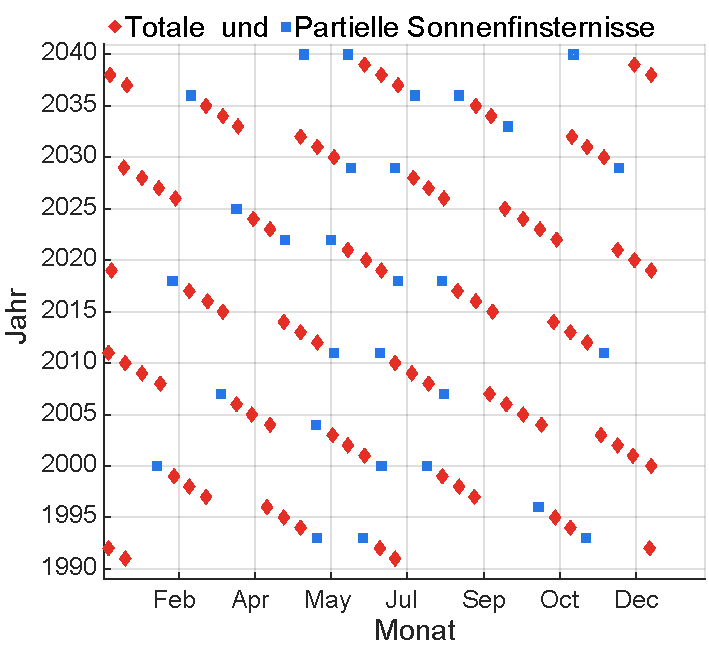
\includegraphics[width=0.5\textwidth]{Sonnenfinsternisse.pdf}}
\hspace{\fill}
\rightfigure{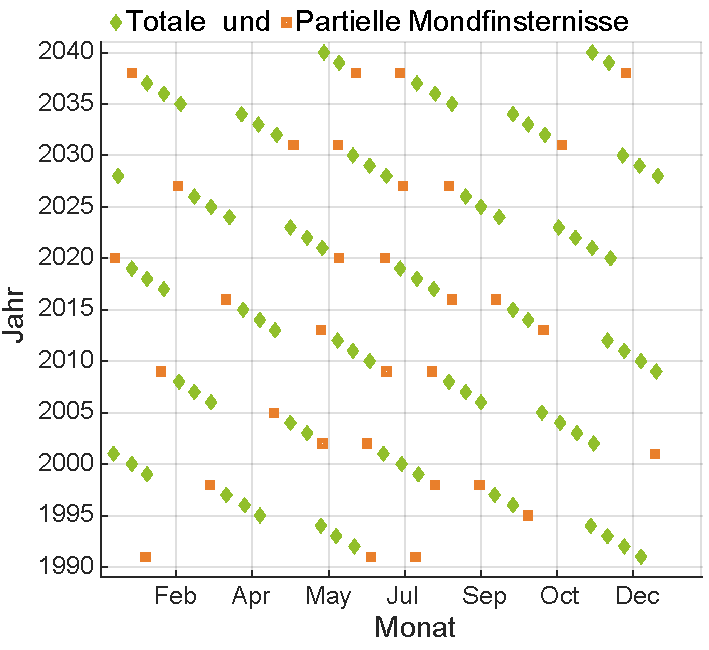
\includegraphics[width=0.5\textwidth]{Mondfinsternisse.pdf}}
\leftcaption[Sonnenfinsternisse 1990--2040.]{Sonnenfinsternisse 1990--2040}\label{abb:hm_Sonnenfinsternisse}
\rightcaption[Mondfinsternisse 1990--2040.]{Mondfinsternisse 1990--2040}\label{abb:hm_Mondfinsternisse}
\end{minipage}
\end{figure}

\medskip \end{sol}
\textcolor{blue} {$\rightarrow$ zur} \probref{hm_MoFi}.\\
\noindent\rule[1ex]{\textwidth}{0.5pt} \newpage

%-----------------------------------------------------------------------------------------------------------


 
%\clearpage
%\clearpage
%\subsection{\mscre--Himmelsmechanik}\label{kap:hm_matlabskripts}

Die \mscre befinden sich im MATLAB-Ordner \texttt{MatlabDateien/hm},
die Hilfsfunktionen im dortigen Unterordner \texttt{Include\-folder} und Daten im Unterordner \texttt{Data}.

Die \mscre befinden sich im MATLAB-Ordner \texttt{MatlabDateien/hm},
die Hilfsfunktionen im dortigen Unterordner \texttt{Include\-folder} und Daten im Unterordner \texttt{Data}.
Es wird empfohlen, entweder die Skripte im GitHub Verzeichnis \githubSN zu benutzen oder sich die komplette Verzeichnisstruktur von \MKc~ runter zu laden und diese und auch das Arbeitsbuch im Hauptverzeichnis Fingeruebungen zu installieren. \\

Wir wollen noch einmal explizit darauf hinweisen, dass die \mscre prim�re der Vermittlung der physikalischen Modelle dienen und keinen Anspruch auf besonders elegante oder effiziente Programmierung erheben. Unser Buch ist ja kein Lehrbuch f�r \matlab-Programmierung. Uns ging es bewusst darum, dass die Skripte gut lesbar sind und das physikalische Modell bzw den physikalischen Gedankengang m�glichst klar abbilden.
Die Leser sind aufgerufen, die Programme nach Belieben zu verbessern und kompakter zu gestalten und diese auch ins GitHub Verzeichnis \githubSN zu stellen.

\subsubsection{Skripte zu Beispielen}\label{mls:hm_bsp_uebungen} %MLSkript1 

\subparagraph{\textbf{Exzentrizit�t Planetenbahnen}}\label{mls:hm_exzentri} %MLSkript2
\begin{longtable}{p{0.33\textwidth}p{0.67\textwidth}}
\hline\noalign{\smallskip}
Skript & Beschreibung \\
\noalign{\smallskip}\svhline\noalign{\smallskip}
\mlhmref{PlanetExzentrizitaeten.m}	& Darstellung der Exzentrizit�ten der Planetenbahnen (auf gro�e Halbachse $a$ normiert).\\
\noalign{\smallskip}\hline\noalign{\smallskip}
\end{longtable}

\subparagraph{\textbf{Analemma}}\label{mls:hm_analemma} %MLSkript3
\begin{longtable}{p{0.33\textwidth}p{0.67\textwidth}}
\hline\noalign{\smallskip}
Skript & Beschreibung \\
\noalign{\smallskip}\svhline\noalign{\smallskip}
\mlhmref{Analemma01.m}        & Analemma auf Basis einer auf der Mittelpunktsgleichung basierenden Keplerl�sung f�r die Sonnenbahn. Exzentrizit�t und Ekliptikschiefe werden variiert (�quinoktium und Ekliptik des Datums). \\
\mlhmref{Analemma02.m}        & Analemmaberechnung (N�herungsrechnung) f�r verschiedene geographische Positionen in Alt-Azimut-Darstellung f�r 24 h. Refraktion und Tagbogenverl�ngerung vernachl�ssigt. Es wird eine einfache auf der Mittelpunktsgleichung basierenden Keplerl�sung f�r die Erdbahn benutzt (�quinoktium und Ekliptik des Datums). \\
\mlhmref{Analemma03.m}        & Analemmaberechnung f�r verschiedene Planeten direkt aus der exzentrischen Anomalie $E$ ohne L�sung der Kepler-Gleichung.\\
\mlhmref{AnalemmaSonne.m}  & Analemmaberechnung der Sonne vom Mond aus auf Basis von auf der Mittelpunktsgleichung basierenden Keplerl�sungen f�r die Sonnen- und Mondbahn.\\
\mlhmref{AnalemmaMond.m}    & Analemmaberechnung f�r Mond von der Erde aus betrachtet auf Basis von auf der Mittelpunktsgleichung basierenden Keplerl�sungen f�r die Sonnen- und Mondbahn.\\
\mlhmref{AnalemmaOkoFit.m}    & Umrechnung einschlie�lich Bildkorrektur des aufgenommenen Analemma von Oberkochen 2019/20 in das horizontale KOS, sowie Darstellung verschiedener theoretisch berechneter Analemma. \\
\mlhmref{AnalemmaFindExz.m}   & Umrechnung einschlie�lich Bildkorrektur des aufgenommenen Analemma von Oberkochen 2019/20 in das horizontale KOS, sowie Fit eines theoretisch berechneten Analemmas mit der Exzentrizit�t e als Parameter. \\
\noalign{\smallskip}\hline\noalign{\smallskip}
\end{longtable}

\subparagraph{\textbf{Sonnenaufgangsberechnung (Methode der quadratischen Interpolation)}}\label{mls:hm_sonnenaufgang} %MLSkript4
\begin{longtable}{p{0.33\textwidth}p{0.67\textwidth}}
\hline\noalign{\smallskip}
Skript & Beschreibung \\
\noalign{\smallskip}\svhline\noalign{\smallskip}
\mlhmref{Sonnenaufgang01.m} & Aufgangs- und Untergangszeiten der Sonne f�r verschiedene geographische Orte (Breite < 60�) und die Tagl�ngen
 iterativ aus der Kepler-Gleichung f�r das ganze Jahr und in der N�he des Jahreswechsels bzw. Mitsommers.\\
\mlhmref{Sonnenaufgang02.m} & Aufgangszeiten auf Basis der Kepler-Gleichung  a) mit einer iterativen Methode (Quadratische 
Interpolation) zur Suche der Nullstellen f�r Auf- und Unterg�nge und b) zum Vergleich auf Basis der ZGL-N�herung.\\
\noalign{\smallskip}\hline\noalign{\smallskip}
\end{longtable}

\subparagraph{\textbf{Vergleich Zeitgleichung}}\label{mls:hm_zeitglgformeln} %MLSkript5
\begin{longtable}{p{0.33\textwidth}p{0.67\textwidth}}
\hline\noalign{\smallskip}
Skript & Beschreibung \\
\noalign{\smallskip}\svhline\noalign{\smallskip}
\mlhmref{ZGL01.m} & ZGL auf Basis einer Mittelpunktsgleichung basierenden Keplerl�sung f�r die Sonnenbahn und Vergleich mit empirischen Werten und den Berechnungen des JPL (�quinoktium und Ekliptik des Datums). \\
\mlhmref{ZGL02.m} & Reihenentwicklung der ZGL.\\
\mlhmref{ZGL03.m} & ZGL auf Basis einer (auf der Mittelpunktsgleichung basierten) Keplerl�sung f�r die Erdbahn und Vergleich mit verschiedenen publizierten N�herungsformeln und den Berechnungen des JPL. \\
\noalign{\smallskip}\hline\noalign{\smallskip}
\end{longtable}
 
\subparagraph{\textbf{Tagbogen-Verl�ngerung}}\label{mls:hm_tagbogenverl} %MLSkript6
\begin{longtable}{p{0.33\textwidth}p{0.67\textwidth}}
\hline\noalign{\smallskip}
Skript & Beschreibung \\
\noalign{\smallskip}\svhline\noalign{\smallskip}
\mlhmref{TagbogenVerlaengerung.m} & Tagbogenverl�ngerung bedingt durch Refraktion und scheinbaren Sonnendurchmesser bei Sonnenaufgang.\\
\noalign{\smallskip}\hline\noalign{\smallskip}
\end{longtable}

%\newpage
\subparagraph{\textbf{Tageslauf Sonne}}\label{mls:hm_tageslauf_sonne} %MLSkript7
\begin{longtable}{p{0.33\textwidth}p{0.67\textwidth}}
\hline\noalign{\smallskip}
Skript & Beschreibung \\
\noalign{\smallskip}\svhline\noalign{\smallskip}
\mlhmref{TageslaufSonne01.m} & Der Tageslauf der Sonne wird nach der N�herungsformel (3.84) berechnet. Die geographische Breite kann variiert werden. Es wird die H�he der Sonne f�r verschieden Jahreszeiten und geographische Breiten dargestellt. Die ZGL wird nicht ber�cksichtigt.
Berechnung des Tagbogenverlaufs (N�herung) der Sonne �ber dem Horizont f�r verschiedene Jahreszeiten und geographische Breiten.\\
\mlhmref{TageslaufSonne02.m} & Tagbogenverlauf der Sonne �ber dem Horizont. (N�herungsformel und zum numerische L�sung. Die geographische Breite kann variiert werden.\\
\noalign{\smallskip}\hline\noalign{\smallskip}
\end{longtable}
 


\subparagraph{\textbf{Berechnung der Aufgangswinkel der Sonne (Verschiedene Orte und Jahreszeiten)}}\label{mls:hm_aufgangswinkel_sonne} %MLSkript8
\begin{longtable}{p{0.33\textwidth}p{0.67\textwidth}}
\hline\noalign{\smallskip}
Skript & Beschreibung \\
\noalign{\smallskip}\svhline\noalign{\smallskip}
\mlhmref{SonnenaufgangZeit.m}    & H�he $h$ und Azimut $\mathcal{A}$ und die Zeit-H�hen-Kurven beim Sonnenaufgang auf Basis einer MPG-Keplerl�sung f�r verschiedene geographische Breiten und verschiedene Jahreszeiten (Wintersonnenwende, Fr�hlingsanfang, Sommersonnenwende, Herbstanfang). Dabei wird die astrometrische H�he $h$ und die durch Refraktion \ua Effekte bedingte \anf{scheinbare} H�he $h'$ berechnet.\\ 
\mlhmref{SonnenaufgangBaabe.m}        & H�he $h$ und Azimut $\mathcal{A}$ und die Zeit-H�hen-Kurven beim Sonnenaufgang auf Basis einer MPG-Keplerl�sung f�r die Erdbahn f�r Baabe (Ostsee). Dabei wird die astrometrische H�he $h$ und die durch Refraktion \ua Effekte bedingte \anf{scheinbare} H�he $h'$ berechnet.\\
\noalign{\smallskip}\hline\noalign{\smallskip}
\end{longtable}
 

\subparagraph{\textbf{Innere Planetenbahnen}}\label{mls:hm_innere_planeten} %MLSkript9
\begin{longtable}{p{0.33\textwidth}p{0.67\textwidth}}
\hline\noalign{\smallskip}
Skript & Beschreibung \\
\noalign{\smallskip}\svhline\noalign{\smallskip}
\mlhmref{InnerePlaneten.m} & Bahnen der inneren Planeten auf Basis der Kepler-Geichung. 
(�quinoktium und Ekliptik des Datums) \\
\mlhmref{VenusTransit01.m} & Koordinaten der Venus und des Merkurs bei Transits. Die Zeiten m�ssen n�herungsweise z.\,B. aus \mlhmref{InnerePlaneten.m} bekannt sein. Die Daten werden mit JPL-Daten verglichen. \\
\mlhmref{VenusTransit02.m} & Bestimmung der Astronomischen Einheit aus den Daten eines Venustransits. a) Parallaxen-Methode nach Halley: Die beobachteten Werte f�r zwei geographische Orte zu einer Zeit UT werden dem Internet entnommen, daraus wird die Parallaxe bestimmt und daraus dann die AE berechnet.  b) Kontaktzeitmethode durch Beobachtung an einem Standort.\\
\noalign{\smallskip}\hline\noalign{\smallskip}
\end{longtable}

\subparagraph{\textbf{�u�ere Planetenbahnen}}\label{mls:hm_aussere_planeten} %MLSkript10
\begin{longtable}{p{0.33\textwidth}p{0.67\textwidth}}
\hline\noalign{\smallskip}
Skript & Beschreibung \\
\noalign{\smallskip}\svhline\noalign{\smallskip}
\mlhmref{AeusserePlaneten.m} & Bahnen der �u�eren Planeten auf Basis der Kepler-Gleichung f�r den Zeitraum 1920--2020. (�quinoktium und Ekliptik des Datums) \\
\noalign{\smallskip}\hline\noalign{\smallskip}
\end{longtable}
 
\subparagraph{\textbf{St�rungsrechnung }}\label{mls:hm_stoerunsgrechnung_planeten} %MLSkript11
\begin{longtable}{p{0.33\textwidth}p{0.67\textwidth}}
\hline\noalign{\smallskip}
Skript & Beschreibung \\
\noalign{\smallskip}\svhline\noalign{\smallskip}
\mlhmiref{VenusExakt.m} & Ekliptikale Koordinaten der Venus auf Basis einer Reihenentwicklung \cite{Montenbruck1999}. \\
\mlhmiref{MarsExakt.m} & Ekliptikale Koordinaten des Mars auf Basis einer Reihenentwicklung \cite{Montenbruck1999}. \\
\mlhmiref{JupiterExakt.m} & Ekliptikale Koordinaten des Jupiters auf Basis einer Reihenentwicklung \cite{Montenbruck1999}. \\
\mlhmiref{SonneExakt.m}  & Ekliptikale Koordinaten der Sonne auf Basis der Newcombschen Theorie \cite{Montenbruck1999}. \\
\mlhmiref{MondExakt.m}. & Geozentrisch-�quatoriale Koordinaten des Mondes auf Basis der Brownschen Theorie \cite{Montenbruck1999}. \\
\mlhmref{SL9numerisch.m} & Bahn des Kometen Shoemaker-Levy 9 bis zu seinem Zusammenprall mit dem Jupiter �ber numerische Integration.
\end{longtable}


\subparagraph{\textbf{Periheldrehung des Merkurs}}\label{mls:hm_perihel_merkur} %MLSkript12
\begin{longtable}{p{0.33\textwidth}p{0.67\textwidth}}
\hline\noalign{\smallskip}
Skript & Beschreibung \\
\noalign{\smallskip}\svhline\noalign{\smallskip}
\mlhmref{PerihelKappa2.m}    & Perihel-Verschiebung f�r ein Potential mit Term $\kappa_2 \neq 0$. \\
\mlhmref{PerihelKappa3.m}    & Perihel-Verschiebung f�r ein Potential mit Term $\kappa_3 \neq 0$. \\
\mlhmref{StoerpotentialMerkur.m}  & St�rpotentiale und Gravitationskr�fte der anderen Planeten auf den Merkur als Ursache der Perihel-Verschiebung des Merkurs nach der Newtonschen Mechanik. \\
\noalign{\smallskip}\hline\noalign{\smallskip}
\end{longtable}

\subparagraph{\textbf{Kometenbahnen}}\label{mls:hm_kometenbahnen} %MLSkript13
\begin{longtable}{p{0.33\textwidth}p{0.67\textwidth}}
\hline\noalign{\smallskip}
Skript & Beschreibung \\
\noalign{\smallskip}\svhline\noalign{\smallskip}
\mlhmref{AsteroidenBahnen.m}   & Bahnen der Asteroiden in heliozentrischen Koordinaten unter Benutzung der Gau�schen Vektoren (�quinoktium und Ekliptik des Datums). \\
\mlhmref{AsteroidenZeit.m}     & Bahn eines Asteroiden als Funktion der Zeit unter fallweiser Benutzung einer parabolischen N�herung. (�quinoktium und Ekliptik des Datums). \\
\mlhmref{KometenBahnen.m}      & Bahnen der Kometen in heliozentrischen Koordinaten unter Benutzung der Gau�schen Vektoren (�quinoktium und Ekliptik des Datums).\\
\mlhmref{KometenZeit.m}        & Bahn eines Kometen als Funktion der Zeit unter fallweiser Benutzung einer parabolischen N�herung (�quinoktium und Ekliptik des Datums). \\
\mlhmref{KometenObsEqu.m}      & Kometenbahnen in Erdn�he als Funktion der Zeit und die Beobachtungsdaten (Rektaszension und Deklination) unter Benutzung von parabolischen N�herungen.\\
\mlhmref{KometenObsHor.m}      & Kometenbahnen in Erdn�he als Funktion der Zeit und die Beobachtungsdaten (Azimut und H�he) unter Benutzung von parabolischen N�herungen.\\
\mlhmref{KometenSL9.m}         & Kepler-Bahn des Kometen D/1993 F2-D (Shoemaker-Levy 9) als Funktion der Zeit und Vergleich mit Werten des JPL \cite{JPL2020} (�quinoktium und Ekliptik des Datums). \\
\mlhmref{KometenHalley.m}      & Bahnen des Kometen Halley von 1986 und 1758 (�quinoktium und Ekliptik Datums). \\
\noalign{\smallskip}\hline\noalign{\smallskip}
\end{longtable}

\subparagraph{\textbf{Gezeiten}}\label{mls:hm_gezeiten} %MLSkript13
\begin{longtable}{p{0.33\textwidth}p{0.67\textwidth}}
\hline\noalign{\smallskip}
Skript & Beschreibung \\
\noalign{\smallskip}\svhline\noalign{\smallskip}
\mlhmref{Gezeitenellipsoid.m}  & Berechnet die Form des Gezeitenellipsoids. \\
\mlhmref{GezeitenReibung01.m}  & Berechnet Parameter der Gezeitenreibung auf der Erde. \\
\mlhmref{GezeitenReibung02.m}  & Berechnet Parameter der Gezeitenreibung auf der Erde mit einem einfachen Hantelmodell.\\
\mlhmref{UmlaufErdeMond.m}     & Simuliert die Bewegung von Erde und Mond um gemeinsamen Schwerpunkt im Laufe eines Monats.\\
%\mlhmref{GezeitenDGLSystem.m}  & L�st das DGLS-System f�r ZKP inklusive Gezeitenreibung.\\
\mlhmref{SimulationAiry.m}     & Simuliert stehende Wellen nach dem Airy-Modell.\\
\noalign{\smallskip}\hline\noalign{\smallskip}
\end{longtable}


\subparagraph{\textbf{Sonnenfinsternisse}} \label{mls:hm_so_fis} %MLSkript14
\medskip
Diese Programme wurden in Teilen auf Basis der C++ Programmstrukturen und der Beschreibung/Erl�uterung in  
"Astronomie mit dem Personal Computer" von Oliver Montenbruck und Thomas Pfleger \cite{Montenbruck1999} entwickelt. 
Genehmigung des Verlages und der Autoren liegt vor.
\begin{longtable}{p{0.33\textwidth}p{0.67\textwidth}}
\hline\noalign{\smallskip}
Skript & Beschreibung \\
\noalign{\smallskip}\svhline\noalign{\smallskip}
\mlhmref{Sonnenfinsternis01.m}    & Zeiten des Neu/Vollmondes in einem bestimmten Zeitraum und bestimmt, ob zu der Neumond/Vollmondzeit eine Sonnen- oder Mondfinsternis stattfinden kann. F�r die Koordinaten Sonne und Mond werden genauere Reihen verwendet. \\
%\mlhmref{PhaseFunc.m} 	& Hilfsfunktion zur Berechnung der Zeiten des Neu/Vollmondes und von Finsternissen.\\
\mlhmref{Sonnenfinsternis02.m}    &  Startet von ungef�hren Neumondzeiten und bestimmt, wann und wo um die Neumondzeit eine Sonnenfinsternis stattfinden kann. F�r die Sonnenfinsternis wird die Zentrallinie der sogenannten maximalen Verfinsterung berechnet.\\
\mlhmref{Sonnenfinsternis03.m}    &  Bestimmt ausgehend vom Neumondzeitpunkt f�r einen gew�hlten Beobachtungsort die Phase, Gr��e und Kontaktzeiten einer Sonnenfinsternis.\\
\noalign{\smallskip}\hline\noalign{\smallskip}
\end{longtable}
 
\subparagraph{\textbf{Lange Zeiten}}\label{mls:hm_lange_zeiten} %MLSkript15
\begin{longtable}{p{0.33\textwidth}p{0.67\textwidth}}
\hline\noalign{\smallskip}
Skript & Beschreibung \\
\noalign{\smallskip}\svhline\noalign{\smallskip}
\mlhmref{ZGL04.m} & Zeitgleichung und Analemma �ber Zeitr�ume von mehreren Jahrtausenden. \\
\noalign{\smallskip}\hline\noalign{\smallskip}
\end{longtable}

\medskip
\subsubsection{Skripte zu verschiedenen �bungen}\label{mls:hm_uebungen} %MLSkript�bungen
\begin{longtable}{p{0.33\textwidth}p{0.67\textwidth}}
\hline\noalign{\smallskip}
Skript & Beschreibung \\
\noalign{\smallskip}\svhline\noalign{\smallskip}
\mlhmref{AbflachungSonne.m}         & Abflachung der Sonne bei Sonnenuntergang als Funktion der H�he.\\
\mlhmref{AnalemmaAnomalie.m}      & Zeitgleichung und Analemma direkt aus der exzentrischen Anomalie.\\
\mlhmref{AufprallgeschwindigkeitKomet.m}        & Aufprallgeschwindigkeit von Kometen/Meteoriten auf der Erde als Funktion verschiedener Parameter.\\
\mlhmref{Besselreihe.m}         & Bessel-Reihe f�r exzentrische Anomalie $E$ f�r verschiedene Exzentrizit�ten $e$ und Summationsgrenzen.\\
\mlhmref{KeplerVergleich.m}         & L�sung der Kepler-Gleichung �ber verschiedene Iterationsverfahren f�r verschiedene Exzentrizit�ten zwischen 0.1, 0.2,.....0.999. Vergleich der Iteration mit Regula falsi und Newton-Raphson f�r verschiedene Anfangswerte der mittleren Anomalie M.\\
\mlhmref{LangzeitJahreszeiten.m}         & Dauer der Jahreszeiten und Energieeintrag der Sonne auf die Nordhemisph�re f�r einen Zeitraum von 8000 Jahren. Einfache Modellierung der Ver�nderungen von Exzentrizit�t, Ekliptikneigung und Richtung der Erdachse.\\
\mlhmref{Mondbahn01.m}         & Mondbahn f�r ein einfaches koplanares ZK-Planet-Mond-System bezogen auf den Zentralk�rper f�r verschiedene Verh�ltnisse der Umlaufzeiten TM (Mond um Planet) und TP (Planet um ZK). \\
\mlhmref{Mondbahn02.m}         & Heliozentrische Mondbahn aus den Ephemeriden.\\
\mlhmref{MarsOpposition.m}         & Marsoppositionen im Zeitraum 2000--2020.\\
\mlhmref{MondErdeSonneApollo8.m}        & Programm berechnet die Positionen von Mond, Erde, Sonne und Apollo 8 am 24.12.1968.\\
\mlhmref{OlympusMons.m}         & Sonnenaufgang auf dem Mars.\\
\mlhmref{PlanetenbahnenKepler.m}         & Bahnen der Planeten Venus bis Jupiter auf Basis der Kepler-Gleichung. Venus-Jupiter-Konjunktion f�r den 22.\ 11.\ 2065 die  (�quinoktium und Ekliptik des Datum). \\
\mlhmref{Refraktion.m}         & Refraktionsberechnung f�r das Kugelschalen-Schichtenmodell und Vergleich mit der Normalrefraktion.\\
\mlhmref{RocheLimit.m}         & Berechnet Roche-Limit und Hill-Sph�ren f�r Planeten unseres Sonnensystems.\\
\mlhmref{SonnenaufgangReinsch.m}         & Analytische Formel f�r Sonnenaufgang nach \cite{Reinsch2003} und Vergleich mit numerischer Berechnung.\\
\mlhmref{SonnenuhrAnalem.m}  & Berechnet Lineatur einer analemmatischen Sonnenuhr f�r G�rlitz.\\
\mlhmref{SimulationAiry.m}  & Simuliert das Airy-Kanal-Modell der dynamischen Theorie der Gezeiten.\\
\mlhmref{TageslaufSonne.m}         & Tageslauf der Sonne mit Ber�cksichtigung der Refraktion $R$ und �ber den Tag ver�nderlicher Deklination $\delta$.\\
\mlhmref{VenusMerkurTransit.m}         & Venustransits am 08.06.2004 und am 06.06.2012.\\
\mlhmref{VerweildauerKomet.m}        & Verweildauer von Kometen in Erdn�he.\\
\mlhmref{Wandsonnenuhr.m}    & Berechnet Lineatur einer Wandsonnenuhr.\\
\mlhmref{ZGLAnalemma.m}      & Zeitgleichung und Analemma auf anderen Planeten (Methode Allison).\\
\mlhmref{ZGLAnalemmaKepler.m}      & Zeitgleichung und Analemma auf anderen Planeten (Methode Montenbruck).\\
\noalign{\smallskip}\hline\noalign{\smallskip}
\end{longtable}

%\newpage
\subsubsection{Hilfsfunktionen}\label{mls:hm_hilfsfunktionen} %MLSkript1 
Einige der Programme wurden in Teilen mit freundlicher Genehmigung der Autoren auf Basis der C++ Programmstrukturen und der Beschreibung/Erl�uterung in \glqq Astronomie mit dem Personal Computer\grqq{} von Oliver Montenbruck und Thomas Pfleger \cite{Montenbruck1999} entwickelt.\\
\begin{longtable}{p{0.33\textwidth}p{0.67\textwidth}}
\hline\noalign{\smallskip}
Skript & Beschreibung \\
\noalign{\smallskip}\svhline\noalign{\smallskip}
Mathematische Funktionen \\
\noalign{\smallskip}\svhline\noalign{\smallskip}
\mlhmiref{CalcAnglesfromXYZ.m}         & Sph�rische Koordinaten aus kartesischen Koordinaten.\\
\mlhmiref{CalcXYZfromAngles.m}         & Kartesische Koordinaten aus sph�rischen Koordinaten.\\
\mlhmiref{Frac.m}                      & Nachkommastellen.\\
\mlhmiref{Modulo.m}                    & Modulus-Funktion.\\
\mlhmiref{R\_x.m}, \mlhmiref{R\_y.m}, \mlhmiref{R\_z.m},     & Rotationsmatrizen bez�glich x,y,z-Achse.\\
\mlhmiref{Stumpff.m}                   & Stumpffsche Funktionen.\\
\noalign{\smallskip}\svhline\noalign{\smallskip}
Hilfsfunktionen f�r Ein- und Ausgabe \\
\noalign{\smallskip}\svhline\noalign{\smallskip}
\mlhmiref{GetColorLines.m}             & L�dt Farbtabelle f�r Linien und graphische Darstellungen.\\
\mlhmiref{StrDMS.m}                    & Umrechnung von Formaten f�r Ausgabe von Winkeln von Dezimal in Grad, Bogenminute, Bogensekunde.\\
\mlhmiref{HMS.m}                       & Umrechnung von Formaten f�r Zeit von Dezimal in hh:mm:ss.s \\
\mlhmiref{StrHMS.m}                    & Umrechnung von Formaten f�r Ausgabe von Zeit von Dezimal in hh:mm:ss.s \\
\mlhmiref{LabelPoints.m}               & Beschriftung von Datenpunkten.\\
\mlhmiref{OrbitParameter.m}            & Einlesen der Bahnparameter der Planeten.\\ 
\mlhmiref{KometParameter.m}            & Einlesen der Bahnparameter der Kometen.\\
\mlhmiref{ImportPlanetParameter.m}     & Einlesen typischer physikalischer Bahnparameter der Planeten und des Mondes.\\

\noalign{\smallskip}\hline\noalign{\smallskip}
Astronomische Funktionen \\
\noalign{\smallskip}\svhline\noalign{\smallskip}
\mlhmiref{Jd.m}                        & Julianisches Datum aus dem Kalenderdatum.\\
\mlhmiref{MJD.m}                       & Modifiziertes Julianisches Datum aus dem Kalenderdatum.\\
\mlhmiref{Jd2JJht.m}                   & Umrechnung von Julianischem Datum in Julianisches Jahrhundert.\\
\mlhmiref{JJht2Jd.m}                   & Umrechnung von Julianischem Jahrhundert in Julianisches Datum.\\
\mlhmiref{GMST.m}                      & GMST (Greenwich Mean Sidereal Time) aus MJD.\\
\mlhmiref{LMST.m}                      & LMST (Local Mean Sidereal Time) aus MJD und geographischer L�nge.\\
\mlhmiref{EpsErde.m}                   & Ekliptikneigung als Funktion der Zeit.\\
\mlhmiref{EAnom.m}                     & Exzentrische Anomalie durch Iteration.\\  
\mlhmiref{Ellip.m}                     & Elliptische Koordinaten aus exzentrischer Anomalie.\\
\mlhmiref{FindRiseSet.m}               & Nullstellensuche Sonnen-Auf- und Untergang im Intervall 0..24 h mit quadratischer Interpolation.\\
\mlhmiref{PQR.m}                       & Multiplikation mit Transformationsmatrix aus Gau�schen Vektoren.\\
\mlhmiref{KometPQR.m}                  & Ekliptikale und �quatoriale Koordinaten von Kometen.\\
\mlhmiref{KometOrbits.m}               & Bahnen der Kometen im Raum.\\
\mlhmiref{PlanetPQR.m}                 & Ekliptikale und �quatoriale Koordinaten von Planeten.\\
\mlhmiref{PlanetOrbits.m}              & Bahnen der Planeten im Raum.\\
\mlhmiref{SonnePQR.m}                  & Ekliptikale und �quatoriale Koordinaten der mittleren Sonne von beliebigen Planeten aus.\\ 
\mlhmiref{KeplerMond.m}                & Mittelpunktsgleichung-L�sung f�r Mond.\\
\mlhmiref{KeplerSonne.m}               & Mittelpunktsgleichung-L�sung f�r Sonne.\\
\mlhmiref{KeplerSonneEx.m}             & Mittelpunktsgleichung-L�sung f�r Sonne -- �quinoktium des Datums und ver�nderliche Exzentrizit�ten.\\
\mlhmiref{KeplerSonneLang.m}           & Mittelpunktsgleichung-L�sung f�r Sonne -- Modellierung f�r gro�e Zeitabst�nde von J2000.\\
%\mlhmiref{SinAlt.m} & Berechnet den Sinus der H�he aus Deklination, Stundenwinkel und Breitengrad.\\ 
\mlhmiref{Convert2Equ.m}               & Umwandlung von ekliptikalen Koordinaten in �quatoriale Koordinaten.\\ 
\mlhmiref{MondExakt.m}                 & Geozentrische Koordinaten des Mondes nach der Brownschen Theorie \cite{Montenbruck1999, Meeus1998}.\\
\mlhmiref{SonneExakt.m}                & Geozentrische Koordinaten der Sonne nach der Newcomschen Theorie \cite{Montenbruck1999, Meeus1998}.\\
\mlhmiref{VenusExakt.m}                & Heliozentrische Koordinaten der Venus nach der St�rungstheorie \cite{Montenbruck1999, Meeus1998}.\\
\mlhmiref{JupiterExakt.m}              & Heliozentrische Koordinaten des Jupiter nach der St�rungstheorie \cite{Montenbruck1999, Meeus1998}.\\
\noalign{\smallskip}\svhline\noalign{\smallskip}
\end{longtable}

\newpage
\subsubsection{Datenfiles} \label{mls:hm_datafiles} %MLSkripteDaten
\begin{longtable}{p{0.4\textwidth}p{0.6\textwidth}}
\hline\noalign{\smallskip}
Skript & Beschreibung \\
\noalign{\smallskip}\svhline\noalign{\smallskip}
csv - Files \\
\noalign{\smallskip}\svhline\noalign{\smallskip}
\mlhmdref{AnalemmaOko2019.csv}              & Analemma-Bilddaten von Aufnahmen in 2019.\\
\mlhmdref{Bahnparameter.csv}                & Bahnparameter f�r �quinoktium und Ekliptik des Datums.\\
\mlhmdref{BahnparameterJ2000.csv}           & Bahnparameter f�r �quinoktium und Ekliptik J2000 \cite{Meeus1998}.\\
\mlhmdref{BahnparameterAbleitung.csv}       & Erste zeitliche Ableitung der Bahnparameter f�r �quinoktium und Ekliptik des Datums.\\
\mlhmdref{BahnparameterJ2000Ableitung.csv}  & Erste zeitliche Ableitung der Bahnparameter f�r �quinoktium und Ekliptik J2000 \cite{Meeus1998}.\\
\mlhmdref{Kometen.csv}                      & Bahnparameter f�r einige ber�hmte Kometen.\\
\mlhmdref{ParaLangzeit.csv}                 & Parameter f�r Langzeitver�nderungen der Bahnparameter der Erde.\\
\mlhmdref{PlanetenFarben.csv}               & Daten f�r Farbkonventionen f�r Planetendarstellungen etc. Wird mit \mlhmiref{GetColorLines.m} eingelesen.\\
\mlhmdref{SL9.csv}                          & Daten f�r Komet Shoemaker-Levy 9 \cite{JPL2020}.\\
\mlhmdref{SonnePos.csv}                     & Parameter f�r St�rungsrechnung der Sonne \cite{Montenbruck1999, Meeus1998}.\\
\mlhmdref{VenusPos.csv} etc.                & Parameter f�r St�rungsrechnung der Planeten \cite{Montenbruck1999, Meeus1998}.\\
\noalign{\smallskip}\svhline\noalign{\smallskip}
dat - Files \\
\noalign{\smallskip}\svhline\noalign{\smallskip}
\mlhmdref{Sonne20040608.dat}         & Koordinaten der Sonne (RA, Deklination) f�r den 08.\,06.\,2004 \cite{JPL2020}.\\
\mlhmdref{Venus20040608.dat}         & Koordinaten der Venus (RA, Deklination) f�r den 08.\,06.\,2004 \cite{JPL2020}.\\
\mlhmdref{ZGLhorizonJPL.dat}         & Daten f�r ZGL 2000 \cite{JPL2020}.\\
\mlhmdref{ZGLempirisch.dat}          & Empirische Daten der ZGL.\\
\noalign{\smallskip}\svhline\noalign{\smallskip}
\end{longtable}



\clearpage
\input{hm/hm_tabellen}
\clearpage
\renewcommand\glslongextraNameAlign{p{36mm}}
\renewcommand\glslongextraDescAlign{p{60mm}}
\clearpage
\bgroup
\small
\printunsrtglossary[type=hm]
\egroup
\clearpage

\fancyhead[RE]{\nouppercase\rightmark}
\bibliography{referenzen}
\clearpage
\fancyhead[RE]{\nouppercase\leftmark}
%%%%%%%%%%%%%%%%%%%%%%%%%%%%%%%%%%%%%%%%%%%%%%%%%%%%%%%%%%%%%%%%%%%%%%%%%%%
%\IfFileExists{footer.tex}{\input{footer.tex}}{}

%\documentclass[makeidx,envcountchap,graybox,deutsch,ngerman,sectrefs]{svmono}
%\documentclass[envcountchap,graybox,deutsch,sectrefs]{svmono}
%%%%% eigene tempor�re Abk�rzungsliste, f�r die Zeit, bis einheitliche Schreibungen bestehen
\usepackage{tempshort}
%%  Von Springer empfohlene Pakete %% 
%%\documentclass[envcountsect,graybox,deutsch,sectrefs]{svmono}
\usepackage{chapterbib}
\usepackage{type1cm}
\usepackage[ansinew]{inputenc}
\usepackage{babel}
\usepackage[pdftex]{graphicx} %PDF-Vektorgrafiken einbinden
\usepackage{newtxtext} %Typischer Springer-Font
\usepackage{newtxmath}
\usepackage{multicol}
\usepackage[bottom]{footmisc} %Platziert alle Fu�noten unten  
\usepackage[nobreak]{cite}
%\usepackage{biblatex}
\usepackage{cancel}
\usepackage[absolute]{textpos}
\usepackage{graphicx}
\usepackage{pdfpages}

%\usepackage{floatrow}
%\usepackage{mwe}
\usepackage[figuresright]{rotating}
\usepackage{bigints}
\let\laplace\relax  % Vermeidung der Fehlermeldung "\laplace already defined."
\usepackage{trfsigns}
\usepackage{amsmath}
\usepackage{tabulary}
\usepackage{tabularx}

%%  Eigene Pakete %%
\usepackage{adjustbox}
\usepackage{wasysym}
\usepackage{gensymb}
\usepackage{float}
\usepackage{caption}
\usepackage[left=5cm,right=4cm,top=3cm,bottom=4cm,includeheadfoot]{geometry}

%\usepackage{wasysym}
%\usepackage{bigints}
%\usepackage{esint}
%\usepackage{relsize,exscale}

\usepackage{mathtools}   % Vermeidung der Fehlermeldung "Undefined control sequence \coloneqq."


% header and footer
\usepackage{fancyhdr}
\pagestyle{fancy}
\fancyhead[LE,RO]\thepage
\renewcommand{\sectionmark}[1]{\markright{\thesection.\ #1}}
%\fancyhead[LO]{\nouppercase\leftmark}
%\fancyhead[RE]{\nouppercase\rightmark}
\fancyhead[LO]{\nouppercase\rightmark}
\fancyhead[RE]{\nouppercase\leftmark}
\fancyfoot{}
% svmono hat offenbar irgendwas merkw�rdig definiert, darum mu� hier verbreitert werden
%\addtolength\headwidth{25pt}
\setlength{\headheight}{25pt}

%% Units
\usepackage{siunitx}
\sisetup{
  locale = US,
  per-mode = reciprocal, %symbol, % | reciprocal | fraction | ?
  exponent-product = \cdot,
  separate-uncertainty,
  %exponent-to-prefix,
  %prefixes-as-symbols = false,
  %list-units = brackets,% | single | repeat
  %range-units = brackets,% | single | repeat
  %multi-part-units = brackets,% | single | repeat
}
\usepackage{chngcntr}
\usepackage{booktabs}
\usepackage{slashed}
\usepackage{listings}
\usepackage{color} %red, green, blue, yellow, cyan, magenta, black, white
%\usepackage{color} %Einfache Farbendefinition -> von Graybox-Option ben�tigt
\usepackage{multirow}
\usepackage{longtable} %Tabellen �ber mehrere Seiten hinweg
\usepackage{framed} % von Graybox-Option ben�tigt
\usepackage[shortlabels]{enumitem} %Erweiterte Aufz�hloptionen
\usepackage{array}
\usepackage[xindy]{imakeidx} %Wortindex und Personenindex erstellen

\usepackage[hyphens]{url}
%\usepackage[breaklinks,colorlinks=true,linkcolor=black,urlcolor=blue,citecolor=black,filecolor=green,hyperfootnotes=false]{hyperref}
\usepackage[                                    %Hyperref erstellt ein Bookmark/Lesezeichen im PDF. siehe https://www.namsu.de/Extra/pakete/Hyperref.html
bookmarksopen=true,															%Das Lesezeichen ist ge�ffnet beim �ffnen der PDF.
bookmarksnumbered=true,                         %Zahlen werden im Bookmark angezeigt.   
plainpages=false,
pdfpagelabels,
colorlinks=true,                                %Links werden farbig dargestellt.
linkcolor=black, citecolor=black, urlcolor=cyan %Farben definieren.
]{hyperref}                                     %Sollte als letztes eingebunden werden, da es sehr viele Verweise und �nderungen erzeugt. Das Packet ist sehr stark, aber auch umfangreich ist. 

%\usepackage[breaklinks,colorlinks=true,linkcolor=black,urlcolor=blue,citecolor=black,filecolor=green,hyperfootnotes=false]{hyperref}
%\usepackage[breaklinks,colorlinks=true,linkcolor=black,urlcolor=blue,citecolor=black,filecolor=green,hyperfootnotes=false
            %pdftex,
            %pdfauthor={Kaschke, Cartarius},
            %pdftitle={Finger�bungen der Physik}
            %pdfsubject={Ein Repetitorium und �bungsbuch zu im Studium wenig behandelten Kapiteln der Physik mit ausf�hrlich behandelten Problemen und MATLAB-Programmen},
            %pdfkeywords={Physik, Mechanik}
            %]{hyperref}
\pdfminorversion=5

\usepackage{hypcap}
\usepackage[record,section=section,stylemods={mcols},automake]{glossaries-extra}
\usepackage{glossary-longextra}
%\usepackage{glossary-bookindex}
%\makeindex
\setglossarystyle{long-name-sym-desc-loc}
\setabbreviationstyle[acronym]{long-short}

\definecolor{killA}{rgb}{.7,.3,.3}
\newcommand\killA[1]{\bgroup\color{killA}{\cancel{#1}}\egroup}
\newcommand\killB[1]{\bgroup\color{cyan!30!black}{\cancel{#1}}\egroup}

% typographisch korrekte Abk�rzungen (needs to be loaded after hyperref)
\usepackage{abbrev}
\newglossary*{bew}{Glossar}
\newglossary*{hm}{Glossar}
\newglossary*{adyn}{Glossar}
\newglossary*{kontmech}{Glossar}
\newglossary*{aero}{Glossar}
\newglossary*{edyn}{Glossar}
\newglossary*{spo}{Glossar}
\newglossary*{optbas}{Glossar}
\newglossary*{optger}{Glossar}
\newglossary*{optatm}{Glossar}
\newglossary*{optspez}{Glossar}
\GlsXtrLoadResources[src={bew/gloss},type=bew]
\GlsXtrLoadResources[src={hm/gloss},type=hm]
\GlsXtrLoadResources[src={adyn/gloss},type=adyn]
\GlsXtrLoadResources[src={kontmech/gloss},type=kontmech]
\GlsXtrLoadResources[src={aero/gloss},type=aero]
\GlsXtrLoadResources[src={spo/gloss},type=spo]
\GlsXtrLoadResources[src={edyn/gloss},type=edyn]
\GlsXtrLoadResources[src={optbas/gloss},type=optbas]
\GlsXtrLoadResources[src={optger/gloss},type=optger]
\GlsXtrLoadResources[src={optatm/gloss},type=optatm]
\GlsXtrLoadResources[src={optspez/gloss},type=optspez]
\glssetcategoryattribute{bew}{indexname}{true}
%\renewcommand\index\newterm
%\newcolumntype{g}[1]{>{\RaggedRight\hspace{0pt}}p{#1}}
%\renewcommand\glslongextraNameAlign{g}
\renewcommand\glslongextraLocationAlign{@{\ ~\ }>{\raggedright}p{\glspagelistwidth}}
\definecolor{gls}{rgb}{.4,.4,.5}
\renewcommand*{\glstextformat}[1]{\textcolor{gls}{#1}}

%Absatzregeln
\clubpenalty = 30000 %Keine einzelnen Absatzzeilen
\widowpenalty = 30000
\setlength{\parindent}{0em} 
\newcolumntype{L}[1]{>{\raggedright\arraybackslash}p{#1}}
\newcolumntype{C}[1]{>{\centering\arraybackslash}p{#1}}
\newcolumntype{R}[1]{>{\raggedleft\arraybackslash}p{#1}}

\usepackage{xstring}

\newcommand\mfile[2]{%
\saveexpandmode\noexpandarg
\StrSubstitute{#2}{_}{\_}[\tmpname]
\restoreexpandmode
\href{MatlabDateien/\chapname/#1\tmpname}{\tmpname}}

%%% Hyperlinks zu MATLAB Dateien
%\newcommand\mlref[1]{\mfile{}{#1}}
%\newcommand\mlinclref[1]{\mfile{IncludeFolder/}{#1}}
%\newcommand\mldataref[1]{\mfile{Data/}{#1}}

%%% .. f�r ein Verzeichnis hoch
%%% . f�r aktuelle Verzeichnis
%% lokal: MatlabDateien/bew
%\newcommand\mlbewref[1]{\href{MatlabDateien/bew/#1}{#1}}
%% git: https://github.com/sn-code-inside/fingeruebungen-physik/tree/main/bew

\newcommand{\mlrefwithindex}[2]{%
  \index[mfiles]{#2}%   <-- Eintrag im M-File-Index mit aktueller Seitenzahl
  \href{https://github.com/sn-code-inside/fingeruebungen-physik/tree/main/#1/#2}{#2}%
}


%\newcommand\mlbewref[1]{\href{https://github.com/sn-code-inside/fingeruebungen-physik/tree/main/bew/#1}{#1}}
%\newcommand\mlbewdref[1]{\href{https://github.com/sn-code-inside/fingeruebungen-physik/tree/main/bew/Data/#1}{#1}}
%\newcommand\mlbewiref[1]{\href{https://github.com/sn-code-inside/fingeruebungen-physik/tree/main/bew/IncludeFolder/#1}{#1}}
%\newcommand\mlkontmechref[1]{\href{https://github.com/sn-code-inside/fingeruebungen-physik/tree/main/kontmech/#1}{#1}}
%\newcommand\mlkontmechdref[1]{\href{https://github.com/sn-code-inside/fingeruebungen-physik/tree/main/kontmech/Data/#1}{#1}}
%\newcommand\mlkontmechiref[1]{\href{https://github.com/sn-code-inside/fingeruebungen-physik/tree/main/kontmech/IncludeFolder/#1}{#1}}
%\newcommand\mlhmref[1]{\href{https://github.com/sn-code-inside/fingeruebungen-physik/tree/main/hm/#1}{#1}}
%\newcommand\mlhmdref[1]{\href{https://github.com/sn-code-inside/fingeruebungen-physik/tree/main/hm/Data/#1}{#1}}
%\newcommand\mlhmiref[1]{\href{https://github.com/sn-code-inside/fingeruebungen-physik/tree/main/hm/IncludeFolder/#1}{#1}}
%\newcommand\mladynref[1]{\href{https://github.com/sn-code-inside/fingeruebungen-physik/tree/main/adyn/#1}{#1}}
%\newcommand\mladyndref[1]{\href{https://github.com/sn-code-inside/fingeruebungen-physik/tree/main/adyn/Data/#1}{#1}}
%\newcommand\mladyniref[1]{\href{https://github.com/sn-code-inside/fingeruebungen-physik/tree/main/adyn/IncludeFolder/#1}{#1}}
%\newcommand\mledynref[1]{\href{https://github.com/sn-code-inside/fingeruebungen-physik/tree/main/edyn/#1}{#1}}
%\newcommand\mledyndref[1]{\href{https://github.com/sn-code-inside/fingeruebungen-physik/tree/main/edyn/Data/#1}{#1}}
%\newcommand\mledyniref[1]{\href{https://github.com/sn-code-inside/fingeruebungen-physik/tree/main/edyn/IncludeFolder/#1}{#1}}
%\newcommand\mloptbasref[1]{\href{https://github.com/sn-code-inside/fingeruebungen-physik/tree/main/optbas/#1}{#1}}
%\newcommand\mloptbasdref[1]{\href{https://github.com/sn-code-inside/fingeruebungen-physik/tree/main/optbas/Data/#1}{#1}}
%\newcommand\mloptbasiref[1]{\href{https://github.com/sn-code-inside/fingeruebungen-physik/tree/main/optbas/IncludeFolder/#1}{#1}}
%\newcommand\mloptspezref[1]{\href{https://github.com/sn-code-inside/fingeruebungen-physik/tree/main/optspez/#1}{#1}}
%\newcommand\mloptspezdref[1]{\href{https://github.com/sn-code-inside/fingeruebungen-physik/tree/main/optspez/Data/#1}{#1}}
%\newcommand\mloptspeziref[1]{\href{https://github.com/sn-code-inside/fingeruebungen-physik/tree/main/optspez/IncludeFolder/#1}{#1}}

\newcommand\mlbewref[1]{\mlrefwithindex{bew}{#1}}
\newcommand\mlbewdref[1]{\mlrefwithindex{bew/Data}{#1}}
\newcommand\mlbewiref[1]{\mlrefwithindex{bew/Include}{#1}}
\newcommand\mlkontmechref[1]{\mlrefwithindex{kontmech}{#1}}
\newcommand\mlkontmechdref[1]{\mlrefwithindex{kontmech/Data}{#1}}
\newcommand\mlkontmechiref[1]{\mlrefwithindex{kontmech/Include}{#1}}
\newcommand\mlhmref[1]{\mlrefwithindex{hm}{#1}}
\newcommand\mlhmdref[1]{\mlrefwithindex{hm/Data}{#1}}
\newcommand\mlhmiref[1]{\mlrefwithindex{hm/Include}{#1}}
\newcommand\mladynref[1]{\mlrefwithindex{adyn}{#1}}
\newcommand\mladyndref[1]{\mlrefwithindex{adyn/Data}{#1}}
\newcommand\mladyniref[1]{\mlrefwithindex{adyn/Index}{#1}}
\newcommand\mledynref[1]{\mlrefwithindex{edyn}{#1}}
\newcommand\mledyndref[1]{\mlrefwithindex{edyn/Data}{#1}}
\newcommand\mledyniref[1]{\mlrefwithindex{edyn/Index}{#1}}
\newcommand\mloptbasref[1]{\mlrefwithindex{optbas}{#1}}
\newcommand\mloptbasdref[1]{\mlrefwithindex{optbas/Data}{#1}}
\newcommand\mloptbasiref[1]{\mlrefwithindex{optbas/Include}{#1}}
\newcommand\mloptspezref[1]{\mlrefwithindex{optspez}{#1}}
\newcommand\mloptspezdref[1]{\mlrefwithindex{optspez/Data}{#1}}
\newcommand\mloptspeziref[1]{\mlrefwithindex{optspez/Include}{#1}}
\newcommand\mloptgerref[1]{\mlrefwithindex{optger}{#1}}
\newcommand\mloptgerdref[1]{\mlrefwithindex{optger/Data}{#1}}
\newcommand\mloptgeriref[1]{\mlrefwithindex{optger/Include}{#1}}
\newcommand\mloptatmref[1]{\mlrefwithindex{optatm}{#1}}
\newcommand\mloptatmdref[1]{\mlrefwithindex{optatm/Data}{#1}}
\newcommand\mloptatmiref[1]{\mlrefwithindex{optatm/Include}{#1}}



\newcommand\mlcmd[1]{\textcolor{cyan}{\texttt{#1}}}

%Grafikregeln
\graphicspath{{hm/graphs/}
	                    	{bew/graphs/}
     						{kontmech/graphs/}
							{hm/graphs/}
							{adyn/graphs/}
							{edyn/graphs/}
							{kontmech/graphs/}
							{spo/graphs/}
							{optbas/graphs/}
							{optger/graphs/}
							{optatm/graphs/}
							{solman/graphs/}
                                                        {aero/graphs}}
\DeclareGraphicsExtensions{.pdf, .png, .jpg, .jpeg}
\def\figname{Abb}
\newcommand\figref[1]{\figname.\ \ref{abb:#1}}
\usepackage[labelfont=bf]{caption}

\usepackage{tocloft}
\usepackage{etoc}
\setlength\cftfignumwidth{30pt}

% Flatterrand links
\cftsetindents{chapter}{0em}{4em}
\cftsetindents{section}{1.5em}{4em}
\cftsetindents{subsection}{3.8em}{4em}

% flacher Rand links
%\cftsetindents{chapter}{0em}{4em}
%\cftsetindents{section}{0em}{4em}
%\cftsetindents{subsection}{0em}{4em}

\newcommand\partitle[1]{
\addcontentsline{toc}{part}{#1}
\begin{titlepage}
  %\vskip 60%\p@
  \begin{center}
    {\LARGE Finger�bungen der Physik -- #1 \par}
    \vskip 3em%
    {\large Michael Kaschke und Holger Cartarius\par}
  \end{center}
\end{titlepage}
}

%\newcommand\mlref[1]{\href{\chapname/matlab/#1}{#1}}
%\newcommand\mlinclref[1]{\href{\chapname/matlab/IncludeFolder/#1}{\color{cyan}{#1}}}

%Neue Kommandos
\newcommand{\lk}{\left(}        %gro�e runde Klammer (links)
\newcommand{\rk}{\right )}      %gro�e runde Klammer (rechts)
\newcommand{\lgk}{\left \{}     %gro�e geschweifte Klammer (links)
\newcommand{\rgk}{\right \}}    %gro�e geschweifte Klammer (rechts)
\newcommand{\lek}{\left [}      %gro�e eckige Klammer (links)
\newcommand{\rek}{\right ]}     %gro�e eckige Klammer (rechts)
\newcommand{\anf}[1]{\glqq#1\grqq}    %Deutsche Anf�hrungszeichen: \anf{}
\newcommand{\defined}{:=}				%Definition
\newcommand{\curl}{\text{\textbf{rot}}\,}	%Rotation-Operator curl()
\newcommand{\ket}[1]{|#1\rangle}		%Quantenmechanischer Zustand
\newcommand{\curvelintri}{\,\overset{\blacktriangle}{\smallfrown}}
\newcommand{\straighttri}{\blacktriangle}
\newcommand{\UT}{\text{UT}}
\newcommand{\UTC}{\text{UTC}}
\newcommand{\JD}{\text{JD}}
\newcommand{\JDE}{\text{JDE}}
\newcommand{\MJD}{\text{MJD}}
\newcommand{\TDT}{\text{TDT}}
\newcommand{\TT}{\text{TT}}
\newcommand{\NVS}{\text{Navier-Stokes-Gleichungen}}
\newcommand{\MWG}{\text{Maxwell-Gleichungen}}
\newcommand{\EMW}{\text{Elektromagnetische Wellen}}
\newcommand{\eMW}{\text{elektromagnetischen Wellen}}
\newcommand{\RT}{\text{Relativit�tstheorie~}}
\newcommand{\au}{\mathrm{AE}}
\newcommand{\ET}{\text{ET}}
\newcommand{\TAI}{\text{TAI}}
\newcommand{\GMST}{\text{GMST}}
\newcommand{\LMST}{\text{LMST}}
\newcommand{\MESZ}{\text{MESZ}}
\newcommand{\KOS}{\text{Koordinatensystem }}
\newcommand{\DGL}{\text{Differentialgleichung }}
\newcommand{\NA}{\text{NA}}
\newcommand{\uA}{\text{u}}  %atomare Masseneinheit
\newcommand{\MOZ}{\text{MOZ}}
\newcommand{\grad}{\text{\textbf{grad}}\,}	%Gradient-Operator grad()
\newcommand{\uproman}[1]{\mathrm{\uppercase\expandafter{\romannumeral#1}}}
\newcommand{\lowroman}[1]{\romannumeral#1\relax}

\newcommand\todo[1]{\textcolor{red}{TODO: #1}}

\renewcommand{\=}[1]{\stackrel{\text{#1}}{=}}  %Schrift �ber Gleich-Zeichen
\renewcommand{\d}{\partial}
\newcommand{\lra}{\Leftrightarrow}  %�quivalenz-Pfeile
\newcommand{\abs}[1]{\left\vert#1\right\vert}     %Betragsklammern
\renewcommand{\Re}{\mathrm{Re}}                          %Realteil
\renewcommand{\Im}{\mathrm{Im}}                          %Imagin�rteil
\renewcommand{\im}{\mathrm{i}}                         %Imagin�re Einheit
\renewcommand{\epsilon}{\varepsilon} 
\newcommand{\keff}{k_\text{eff}}
\newcommand{\con}{\text{const}}
\newcommand{\conv}{\vec{const}}
\newcommand{\PL}{\mathcal{P}_}
\newcommand{\artanh}{\mathrm{artanh}}
% QED-Symbol im text- bzw. Mathemodus
\newcommand{\textqed}{\hfill ~ $\square$}
\newcommand{\mmqed}{\tag*{$\square$}}

\newcommand{\fa}{(\textbf{a}) }
\newcommand{\fb}{(\textbf{b}) }
\newcommand{\fc}{(\textbf{c}) }
\newcommand{\fd}{(\textbf{d}) }
\newcommand{\fe}{(\textbf{e}) }
\newcommand{\ff}{(\textbf{f}) }

\newcommand{\iF}{im Folgenden~}
\newcommand{\iA}{im Allgemeinen~}


\DeclareMathOperator\divv{div}
\DeclareMathOperator\res{Res}
\DeclareMathOperator{\sech}{sech}
\DeclareMathOperator\sgn{sgn}

% f�r Appendix - MATLAB Referenz
\newcommand{\rotv}{\vec{rot}\,}
\newcommand{\gradv}{\vec{grad}\,}
\newcommand{\nablav}{\vec{\nabla}\,}

\newcommand{\ceil}{\mathrm{ceil}}
\newcommand{\sinc}{\mathrm{sinc}}
\newcommand{\diag}{\mathrm{diag}}
\newcommand{\sign}{\mathrm{sign}}
\newcommand{\length}{\mathrm{length}}
\newcommand{\sort}{\mathrm{sort}}
\newcommand{\summ}{\mathrm{sum}}
\newcommand{\asin}{\mathrm{asin}}
\newcommand{\acos}{\mathrm{acos}}
\newcommand{\atan}{\mathrm{atan}}
\newcommand{\prodd}{\mathrm{prod}}
\newcommand{\median}{\mathrm{mediab}}
\newcommand{\mean}{\mathrm{mean}}
\newcommand{\std}{\mathrm{std}}
\newcommand{\eye}{\mathrm{eye}}
\newcommand{\zeros}{\mathrm{zeros}}
\newcommand{\ones}{\mathrm{ones}}
\newcommand{\rand}{\mathrm{rand}}
\newcommand{\inline}{\mathrm{inline}}
\newcommand{\modd}{\mathrm{mod}}
\newcommand{\floor}{\mathrm{floor}}
\newcommand{\round}{\mathrm{round}}
\newcommand{\rem}{\mathrm{rem}}
\newcommand{\sqrtt}{\mathrm{sqrt}}
\newcommand{\triu}{\mathrm{triu}}
\newcommand{\tril}{\mathrm{tril}}
\newcommand{\size}{\mathrm{size}}
\newcommand{\dett}{\mathrm{det}}
\newcommand{\inv}{\mathrm{inv}}
\newcommand{\rank}{\mathrm{rank}}
\newcommand{\rref}{\mathrm{rref}}
\newcommand{\eig}{\mathrm{eig}}
\newcommand{\poly}{\mathrm{poly}}
\newcommand{\lu}{\mathrm{lu}}
\newcommand{\qr}{\mathrm{qr}}
\newcommand{\quaddd}{\mathrm{quad}}
\newcommand{\fzero}{\mathrm{fzero}}
\newcommand{\roots}{\mathrm{roots}}
\newcommand{\odezd}{\textcolor{mygreen}{\texttt{ode23}}}
\newcommand{\odevf}{\textcolor{mygreen}{\texttt{ode45}}}
\newcommand{\odeeds}{\textcolor{mygreen}{\texttt{ode13s}}}
\newcommand{\odeefs}{\textcolor{mygreen}{\texttt{ode15s}}}
\newcommand{\ddezd}{\textcolor{mygreen}{\texttt{dde23}}}
\newcommand{\onlineZ}{online verf�gbaren Zusatzmaterialien{}}
\newcommand{\MKc}{\url{https://www.fingeruebungen-physik.de}{}}
\newcommand{\linklsg}{\href{https://www.fingeruebungen-physik.de}{\textcolor{blue} {$\rightarrow$ L�sungsteil.}}}
\newcommand{\githubSN}{\url{https://github.com/sn-code-inside/fingeruebungen-physik}{}\,\,}

\newcommand{\FT}{\mathcal{F}} %Fourier-Transformierte

% Aufz�hlung der L�sungen der Teilaufgaben
\newlist{subprobs}{enumerate}{1}
\setlist[subprobs]{
  label= \textbf{\textit{Teilaufgabe}} \textbf{\textit{\arabic*:}} \protect\thissubprob,
  ref=\arabic*, itemsep=\baselineskip, align=left}
\newcommand{\subprob}[1]{
  \def\thissubprob{\textbf{\textit{#1}}}\item ~\vspace{0.2\baselineskip} \newline}

\renewenvironment{example}[1]{
\refstepcounter{example}\par\medskip
\begin{shaded} 
\begin{samepage}
\noindent \textbf{\textit{Beispiel~\theexample: {#1}}}\\ 
\noindent{\color{black} \rule{\textwidth}{0.2 mm}}
\end{samepage}
}{\end{shaded}
\noindent{\color{black} \rule{\textwidth}{0.2 mm}}
} % or snugshade
\definecolor{shadecolor}{gray}{0.95}
\definecolor{mygreen}{RGB}{28,172,0} % color values Red, Green, Blue
\definecolor{mylilas}{RGB}{170,55,241}

\newenvironment{infobox}[1]{
     \begin{shaded} 
     \begin{samepage}
\noindent{\color{black} \rule{\textwidth}{0.2 mm}}
     \end{samepage}
}{\end{shaded}
\noindent{\color{black} \rule{\textwidth}{0.2 mm}}
} 
\definecolor{shadecolor}{gray}{0.95}
\definecolor{mygreen}{RGB}{28,172,0} % color values Red, Green, Blue
\definecolor{mylilas}{RGB}{170,55,241}


\newenvironment{nebenrechnung}[1]{
\begin{shaded} 
\begin{samepage}
\noindent\textbf{Nebenrechnung: \\} 
\noindent{\color{black} \rule{0.1\columnwidth}{0.2mm} \\}
\end{samepage}
}{\end{shaded}
\noindent{\color{black} \rule{0.1\columnwidth}{0.2mm} \\}
} % or snugshade
\definecolor{shadecolor}{gray}{0.95}
\definecolor{mygreen}{RGB}{28,172,0} % color values Red, Green, Blue
\definecolor{mylilas}{RGB}{170,55,241}

\newenvironment{merksatz}[1]{
\begin{shaded} 
\begin{samepage}
\noindent\textbf{Merke:\\} 
\noindent{\color{black} \rule{0.9\columnwidth}{0.2mm} \\ \\}
\end{samepage}
}{\end{shaded}
\noindent{\color{black} \rule{0.9\columnwidth}{0.2mm} \\}
} % or snugshade


\lstset{language=Matlab,%
    %basicstyle=\color{red},
    %basicstyle={\linespread{0.9}\ttfamily},
    basicstyle=\footnotesize\ttfamily,
    breaklines=true,%
    morekeywords={matlab2tikz},
    keywordstyle={\small \color{mygreen}},%
    morekeywords=[2]{1}, keywordstyle=[2]{\small\color{black}},
    identifierstyle={\small \color{black}},%
    stringstyle={\small\color{mylilas}},
    commentstyle={\small\color{mylilas}},%
    showstringspaces=false,%without this there will be a symbol in the places where there is a space
    numbers=left,%
    numberstyle={\tiny \color{black}},% size of the numbers
    numbersep=9pt, % this defines how far the numbers are from the text
    emph=[1]{for,end,else,break, function},emphstyle=[1]\small \color{blue}, %some words to emphasise
    emph=[2]{odeset},emphstyle=[2]\small \color{mygreen}, %some words to emphasise
    %emph=[2]{word1,word2}, emphstyle=[2]{style},    
}

%\bibliographystyle{spphys.bst}

%Trennregeln f�r spezielle Worte
%\hyphenation{Fresnel \matlab �qui-nok-ti-um}

\DeclareSIUnit\erg{erg}
\DeclareSIUnit\cal{cal}
\DeclareSIUnit\celsius{C}
\DeclareSIUnit\m{M}
\DeclareSIUnit\kel{K^{-4}}

%Stichwort- und Personenverzeichnis
\makeindex[title=Stichwortverzeichnis] % Create the default index
\makeindex[name=personen,title=Personenverzeichnis] % Create an index named 'personen'
\newcommand{\indexp}[1]{\index[personen]{#1}}
\makeindex[name=mfiles,title=MATLAB-Skriptverzeichnis,columns=2]

% list of exercises
\newcommand{\loxname}{\Large �bungsverzeichnis}  % einheitliche Gr��e Large
\newlistof[chapter]{prob}{lox}\loxname
\newcommand\uebung[3][]{\label{prob:#2}%
\addcontentsline{lox}{prob}{\protect\numberline{}{\probRef{#2}:~#3#1}}%
\textbf{#1#3}\\[\baselineskip]}
\makeatletter
\renewcommand{\l@prob}{\@dottedtocline{1}{0em}{0em}}
\makeatother

\newcommand\einfach{\uebung[~$\ast$~~]}
\newcommand\mittel{\uebung[~$\ast\,\ast$~~]}
\newcommand\schwierig{\uebung[~$\ast\,\ast\,\ast$~~]}
\newcommand\zusatz{\uebung[~$\ast\,\ast\,\ast\,!$~~]}
%\newcommand\einfach{\uebung[~\textbf{*}~~]}
%\newcommand\mittel{\uebung[~\textbf{*\,*}~~]}
%\newcommand\schwierig{\uebung[~\textbf{*\,*\,*}~]}
%\newcommand\zusatz{\uebung[~\textbf{*\,*\,*\,!}~~]}
\usepackage[atend]{bookmark}
%\BookmarkAtEnd{%
%\bookmarksetup{startatroot}\bookmark[level=0,named=\loxname]{}}

\newcommand\kapitel[1]{Kapitel \ref{kap:#1}}
%\newcommand\kap[1]{Kap.\ \ref{kap:#1}}
\newcommand\kap[1]{Kap. \ref{kap:#1}}

\begin{document}
% customize prob and sol in svmono
\makeatletter
%\counterwithin*{chapter}{part}

\spn@wtheorem{prob}{\bgroup\exercisename\egroup}{\bfseries}{\rmfamily}
\makeatother
\renewenvironment{sol}[1]{\par\addvspace{6pt}\noindent\phantomsection{\textbf{L�sung \ref{#1}}} \ignorespaces}{\par\addvspace{6pt}}
\newcommand\probRef[1]{�bung \ref{prob:#1}}
\renewcommand\probref[1]{\textbf{\probRef{#1}}}
\newcommand\lsgref[1]{L�sung \ref{lsg:#1}}

\newcommand\sbullet[1][.5]{\mathbin{\vcenter{\hbox{\scalebox{#1}{$\bullet$}}}}}

\setcounter{table}{0}


%%%%%%%%%%%%%%%%%%%%%%%%%%%%%%%%%%%%%%%%%%%%%%%%%%%%%%%%%%%%
\chapter{Astrodynamik}\label{chap:adyn}
\def\chapname{adyn}
\bibliographystyle{spphys}
%\begin{bibunit}[spphys]
\input{adyn/adyn_motivation}
\newpage
\section{Grundlagen der Raketenphysik} \label{kap:adyn_rockets}

Um einen k�nstlichen Satelliten von der Erdoberfl�che (oder von einem anderen Himmelsk�rper) ins Weltall zu bringen, muss man diesen nach den  Gesetzen der Himmelsmechanik (Kap. \ref{chap:hm}) auf eine bestimmte Geschwindigkeit bringen. Wie bereits erw�hnt, war es bereits Oberth, Ziolkowski und Goddard klar, dass ein Kanonenschuss, wie von Jules Verne beschrieben, als Antrieb zum Mond nicht funktionieren w�rde (Wir rechnen das in \probref{adyn_canonball} nach.). Deswegen kam f�r einen Flug, der auch im nahezu luftleeren Raum stattfindet, nur ein Raketentriebwerk in Frage. 

\subsection{Raketen-Gleichung}\label{kap:adyn_rocketequ} \index{Raketen-Gleichung|textbf}

\begin{figure}[H]
	\includegraphics[width=\textwidth]{Rockets01.pdf} 
	\caption[Zur Herleitung der Raketen-Gleichung.]{Zur Herleitung der Raketen-Gleichung. Die Rakete hat zum Zeitpunkt $t$ die Masse~$m$ (inklusive Treibstoff) und die Geschwindigkeit $\vec{v}_\text{R}$. Nach einem kleinen Zeitinterval $\D t$ hat sich die Gesamtmasse $m$ um die Masse der ausgesto�enen Treibgase $\D m_\text{G} > 0$ verringert. Im Bild sind Raketen- und Treibgasgeschwindigkeit $\vec{v}_\text{R}$ und $\vec{v}_\text{G}$ kollinear  eingezeichnet, das muss \ia nicht der Fall sein. Man beachte, dass die �nderung der Gesamtmasse $\D m$ negativ und durch $\D m = - \D m_\text{G}$ gegeben ist.}
	\label{abb:adyn_rockets01}
\end{figure}

Ein Raketentriebwerk funktioniert nach dem R�cksto�prinzip\index{R�cksto�prinzip} und dieses wiederum auf der Impulserhaltung\index{Impulserhaltung}. Wir betrachten zun�chst eine solche Rakete im luftleeren Raum in einem Kraftfeld wie \zb dem Gravitationsfeld der Erde (\figref{adyn_rockets01}). Die Rakete verliert w�hrend der relativ kurzen Brenndauer ihres Raketentriebwerks an Masse\footnote{Bei einem chemischen Raketenantrieb ist der Brennstoffverbrauch sehr hoch, deshalb f�llt dieser Effekt viel st�rker ins Gewicht als \zb bei einem nuklearen Raketentriebwerk, das das auszusto�ende Gas durch eine Kernreaktion erhitzt. Noch weniger Treibstoff verbrauchen elektrische Raketentriebwerke, zu denen zum Beispiel der Ionenantrieb z�hlt. Wir werden uns im wesentlichen auf chemische Raketentriebwerke fokussieren. Im \kap{adyn_maneuvers} werden wir kurz auf die Unterschiedlichkeit der Man�ver eingehen, die sich f�r die verschiedenen Triebwerksarten ergeben.} (dabei steigt bei gleich bleibendem Antrieb die Beschleunigung), wir haben es also mit einem dynamischen System sich ver�ndernder Masse zu tun, wie wir es \zb auch schon im Kapitel 1.3.5.5 in Band I untersucht haben. Man muss die  Newtonsche Bewegungsgleichung f�r solche Systeme in ihrer allgemeinen Form benutzen:
\begin{align}
    \vec{F}_\text{ext} = \frac{\D \vec{p}_\text{ges}}{\D t}  = \frac{\D \vec{p}_\text{R}}{\D t} + \frac{\D \vec{p}_\text{G}}{\D t} \,,\label{eq:adyn_rockets01}
\end{align}
worin der Gesamtimpuls $\vec{p}_\text{ges}$ aus $\vec{p}_\text{R}$ f�r den Impuls der Rakete und $\vec{p}_\text{G}$ den Impuls der ausstr�menden Gase besteht. Die Gasgeschwindigkeit der ausstr�menden Gase $\vec{v}_\text{G}$ wird gemessen im \textit{mitbewegten} Koordinatensystem, welches sich auf den Ort der mitbewegten D�se (oder genauer auf den Schwerpunkt der Rakete) bezieht. Da es verschiedene, die Gasgeschwindigkeit negativ beeinflussende Faktoren gibt, ersetzt man \ia $\vec{v}_\text{G}$ durch $\vec{v}_\text{G,eff}$, worin $\vec{v}_\text{G,eff}$ eine effektive Ausstr�mgeschwindigkeit der Verbrennungsgase ist. F�r diese effektive \textit{Strahlgeschwindigkeit} oder \textit{Schubgeschwindigkeit}\index{Schubgeschwindigkeit}\index{Strahlgeschwindigkeit} gilt $|\vec{v}_\text{G,eff}| < |\vec{v}_\text{G}|$. Als ein typisches Beispiel sei ein sogenanntes kryogenes $\text{H}_2$-$\text{O}_2$-Triebwerk genannt, das theoretisch eine Strahlgeschwindigkeit von \ca $v_\text{G}\approx \SI{5100}{\metre\per\second}$ erm�glichen sollte, dessen effektive Schubgeschwindigkeit $v_\text{G,eff}$ aber nur \ca $\SI{4400}{\metre\per\second}$ betr�gt \cite{Messerschmid2017}. Wir schreiben im Folgenden aber der K�rze wegen immer $\vec{v}_\text{G} $, auch wenn wir darunter  $\vec{v}_\text{G,eff} $ verstehen wollen.\\
Zum Zeitpunkt $t$ sei noch kein Gas ausgetreten, dann gilt:
\begin{align}
    \vec{p} \lk t\rk &= \vec{p}_\text{R}(t) =  m\,\vec{v}_\text{R}\,. \label{eq:adyn_rockets01a}
\end{align}
Zum Zeitpunkt $t + \D t$ hat sich die Gesamtmasse um Gas der Menge $\D m = -\D m_\text{G}$ verringert\footnote{Man beachte, dass $\D m < 0$, mithin $\D m_\text{G} > 0 $ ist!}, dann gilt im eingezeichneten \textit{festen} \KOS, das als Inertialsystem mit dem Ursprung im Erdmittelpunkt angenommenen werden kann:
\begin{align}
    \vec{p} \lk t + \D t \rk &= \vec{p}_\text{R}\lk t +\D t \rk \,+ \, \vec{p}_\text{G} \lk t + \D t \rk \nonumber \\
		                   &= \lk m + \D m \rk \lk \vec{v}_\text{R} + \D \vec{v}_\text{R}\rk + \D m_\text{G} \lk \vec{v}_\text{R} + \vec{v}_\text{G} \rk \nonumber \\
										 	 &= m\,\vec{v}_\text{R} \,+\,\killA{\D m \, \vec{v}_\text{R}} + m \,\D \vec{v}_\text{R}\, - \,\cancel{\D m\,\D v_\text{R}} \,\, \killA{\,-\, \D m\,\vec{v}_\text{R}} \, - \,\D m\,\vec{v}_\text{G} \nonumber \\
											 &= m\,\vec{v}_\text{R} + m \,\D \vec{v}_\text{R} - \D m\,\vec{v}_\text{G} \,.  \label{eq:adyn_rockets01b}
\end{align}

Wir bilden aus $\D [\vec{p}\lk t + \D t \rk - \vec{p}\lk t\rk]$ den Differentialquotienten �ber die Zeit und erhalten aus \eqref{eq:adyn_rockets01} bis \eqref{eq:adyn_rockets01b} im kr�ftefreien Raum wegen der Impulserhaltung 
\begin{align}
   \frac{\D \vec{p}_\text{ges}}{\D t } = 0 ~~~~\rightarrow~~~~ m\,\dot{\vec{v}}_\text{R} - \dot{m}\,\vec{v}_\text{G} = 0\,. \label{eq:adyn_rockets02}
\end{align}
F�r $\vec{F}_\text{ext} = 0$ erhalten wir also die Raketen-Gleichung f�r den kr�ftefreien Raum:
\begin{align}
    m\,\dot{\vec{v}}_\text{R} = \dot{m}\,\vec{v}_\text{G} = \vec{F}_\text{S} \,. \label{eq:adyn_rockets03}
\end{align}
Der Term $\vec{F}_\text{S}$ ist die sogenannte \textit{Schubkraft}\index{Schubkraft}\glslink{thrust}.

Im Normalfall werden als externe Kr�fte vor allem die Gravitation $\vec{F}_\text{G}$ und die Reibung $\vec{F}_\text{D}$ wirken.\footnote{Wir benutzen hier den Subskript D f�r engl. \emph{Drag}\index{Drag}\glslink{drag}, um Verwechslungen mit dem Subskript R f�r Rakete zu vermeiden.}

Wir k�nnen \eqref{eq:adyn_rockets03} f�r $|\vec{v}_\text{G}| = \con$ leicht integrieren und gehen dabei einfacherweise zu skalaren Gr��en �ber, wobei wir vereinfachend annehmen, dass $\vec{v}_\text{R}$ antiparallel zu $\vec{v}_\text{G}$ ist. Das ergibt:
\begin{align*}
    \D v_\text{R} = - \frac{\D m}{m}\,v_\text{G}\,,
\end{align*}
worin die Zeit nicht explizit enthalten ist, so dass die Integration 
\begin{align}
    \Delta v_\text{R} = v_\text{R}\lk t_f\rk - v_\text{R}\lk t_0\rk = - v_\text{G}\,\ln \frac{m(t_f)}{m(t_0)} = v_\text{G}\,\ln \frac{m_0}{m_f} \label{eq:adyn_rocketequ} \,.
\end{align}
ergibt. Das ist die ber�hmte \gls{rocketequ}\index{Raketen-Gleichung}\footnote{Diese Gleichung wird in der Literatur h�ufig auch als Ziolkowski-Gleichung\index{Ziolkowski-Gleichung|textbf} bezeichnet.}, die die Geschwindigkeits�nderung im freien Raum �ber eine Brennphase des Triebwerks mit konstanter Strahlgeschwindigkeit\index{Strahlgeschwindigkeit} $v_\text{G}$ hinweg angibt, worin $m_0$ die (Start-)Masse zum Zeitpunkt $t_0$ und $m_f$ die Masse zum Zeitpunkt $t_f$ sind. Diese Geschwindigkeits�nderung $\Delta v_\text{R}$, h�ufig auch nur $\Delta v$ geschrieben, ist f�r die Betrachtung der Dynamik eines Raumschiffs/einer Rakete die wichtigste Gr��e und wird \emph{Antriebsverm�gen} \index{Antriebsverm�gen} oder \emph{charakteristische Geschwindigkeit}\index{Geschwindigkeit!charakteristische} genannt.
Die zugeh�rige Massen�nderung ist gegeben durch 
\begin{align}
    \Delta m = m_0 \lk  1- e^{-\frac{\Delta v_\text{R}}{\,v_\text{G}}}\rk = m_f\lk e^{\frac{\Delta v_\text{R}}{\,v_\text{G}}} -1\rk  \label{eq:adyn_rockets05} \,.
\end{align}
Der Gesamtimpuls zum Zeitpunkt $t_\text{end}$ nach dem sogenannten \gls{Brennschluss}\index{Burn-out}\index{Brennschluss} ist gegeben durch
\begin{align}
    p_\text{tot} \lk t_f \rk = \int\limits_0^{t_f} F_\text{S} \lk t'\rk\,\D t' \,,  \label{eq:adyn_rockets06}
\end{align}
\bzw $p_\text{tot} = F_\text{S}\,t_f$ f�r konstanten Schub. In der Raketentechnik benutzt man h�ufig den spezifischen Impuls\index{Impuls!spezifischer} $I_\text{S}$ (in $\SI{}{\second}$), der definiert ist als Schubkraft geteilt durch den mit der Erdbeschleunigung $g$ multiplizierten Treibstoffdurchsatz $\dot{m}_\text{T}$ (in $\SI{}{\N\per\second}$)\,:
\begin{align}
    I_\text{S} = \frac{F_\text{S} }{g\,\dot{m}_\text{T}} = \frac{F_\text{S} \,t_f}{m_\text{T}\,g} = \frac{p_\text{tot}}{m_\text{T}\,g}\,.  \label{eq:adyn_rockets07}
\end{align}
In \figref{adyn_rockets02} haben wir die numerische Berechnung eines Raketenfluges von der Erdoberfl�che dargestellt. Man erkennt die initiale Beschleunigungsphase bis zum Brennschluss, die bei den angegebenen Parametern (Treibstoffmasse $m_\text{T}(t_0) =\SI{2.688e6}{\kg}$, $v_\text{G}=\SI{3000}{\metre\per\second}$) nur wenig mehr als 3 min dauert. 

\begin{figure}
	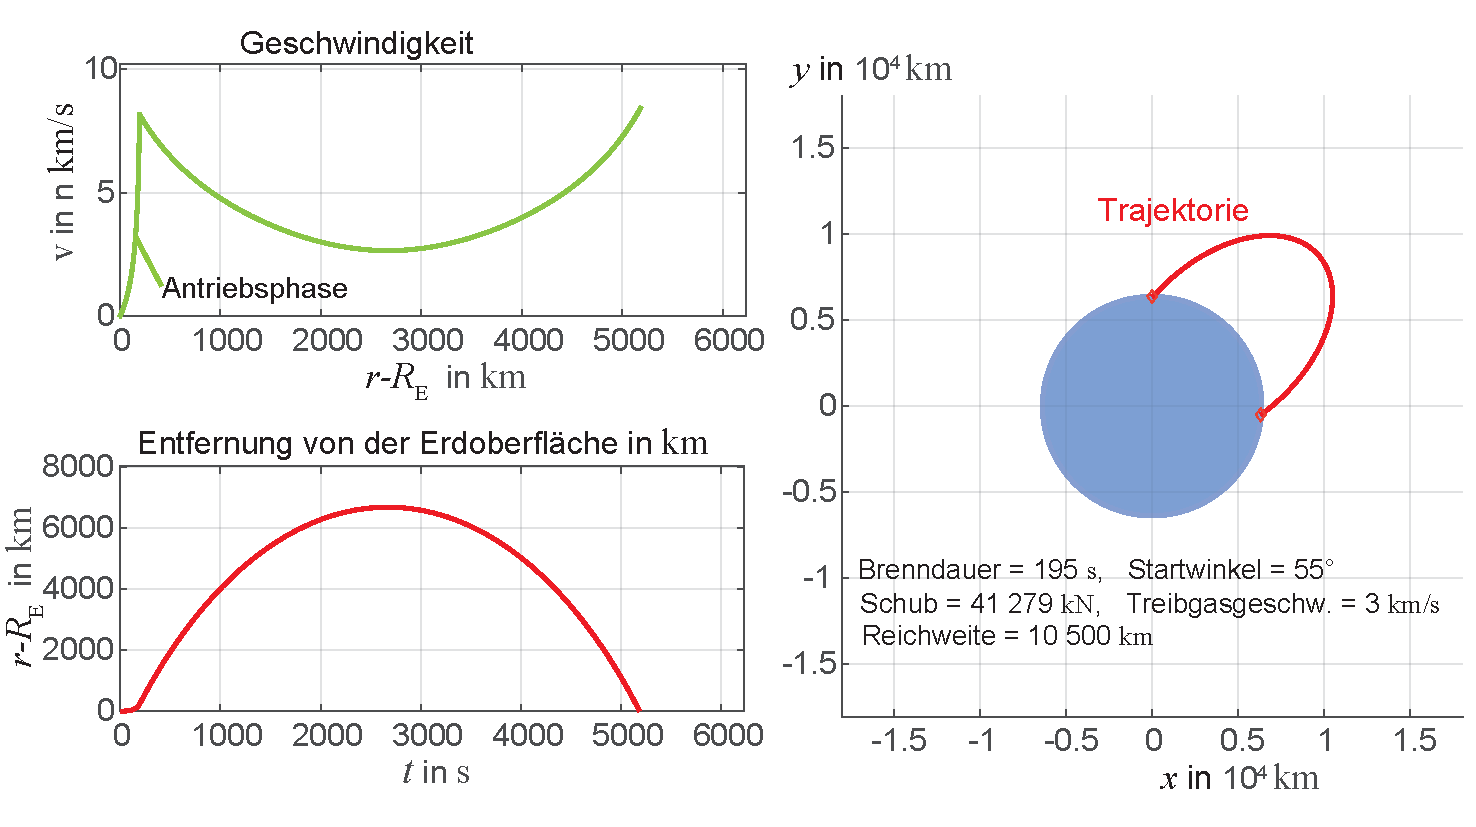
\includegraphics[width=\textwidth]{Rockets02.pdf} 
	\caption[Dynamik einer einstufigen von der Erdoberfl�che gestarteten Rakete.]{Numerische Berechnung der Dynamik einer einstufigen von der Erdoberfl�che gestarteten Rakete. Die numerische Rechnung (siehe \mscr\ \mladynref{Raketenstart01.m}) verwendete die vollst�ndige Bewegungsgleichung \eqref{eq:adyn_rockets01}, \dh ber�cksichtigt auch die Verringerung der Gravitationskraft in gr��eren H�hen, aber keine Reibung der Erdatmosph�re. Das werden wir in \kap{adyn_reentry} anschauen. Man erkennt, dass bei den gew�hlten Parametern die Rakete nach dem Brennschluss eine elliptische ballistische Bahn durchl�uft, die also keine volle Erdumrundung ergibt (adaptiert nach \cite{Hasbun2018})}.
	\label{abb:adyn_rockets02}
\end{figure}

\subsection{Nutzlast-�berlegungen}\index{Nutzlast}\index{Payload}\label{kap:adyn_payload}

\subsubsection{Wirkungsgrad}\label{kap:adyn_efficiency}

F�r das Design von Raketensystemen sind neben dem Schub \bzw dem erreichbaren Gesamtimpuls noch zwei �berlegungen wichtig. Zum einen der Wirkungsgrad und zum anderen die maximale Masse, die sich mit einer Rakete auf eine bestimmte Geschwindigkeit und damit auf eine bestimmte Bahn bringen l�sst. Wir wenden uns zun�chst dem Wirkungsgrad zu und betrachten den wichtigen inneren Wirkungsgrad. Dieser gibt an, wie viel Treibstoffenergie ben�tigt wird, um eine bestimmte Schubenergie zu erzeugen:
\begin{align}
    \eta_\text{int} = \frac{\frac{1}{2}{m_\text{T}\, v_\text{G}{}^2}}{E_\text{T}}  \label{eq:adyn_rockets08}\,.
\end{align}
Dieser Wirkungsgrad bestimmt, wie gro� $v_\text{G}$ und damit das Antriebsverm�gen $\Delta\, v$ bei einer bestimmten Treibstoffmenge $m_\text{T}$ (mit entsprechendem Energieinhalt $E_\text{T}$) letztendlich werden kann.

\subsubsection{Grenzen einstufiger Raketen}\label{kap:adyn_onestagerockets}

Wenn man sich Gleichung \eqref{eq:adyn_rocketequ} anschaut, k�nnte man auf die Vermutung kommen, dass man die Anfangsmasse (Startmasse) $m_1$ nur hinreichend gro� machen m�sste, um ein Raumschiff einer Masse $m_2$ auf eine beliebig gro�e Geschwindigkeit zu bringen. Dem ist aber nicht so. Wir betrachten dazu die Massenverh�ltnisse in einem Raketensystem genauer. Es gilt:
\begin{align}
\begin{split}
    t = t_0 : ~~ m_0 &= m_\text{S} + m_\text{L} + m_\text{T} \; , \\
		t = t_f : ~~ m_\text{f} &= m_\text{S} + m_\text{L} \;,
\end{split} \label{eq:adyn_rockets09}
\end{align}
worin $m_\text{S}$ die Masse der Struktur (Triebwerk, Schale \usw), $ m_\text{L}$ die Nutzlast (englisch \textit{Payload}) \glslink{payload} und $m_\text{T}$ die Treibstoffmasse jeweils zum Zeitpunkt $t=0$ sind.
Wir definieren das Nutzlastverh�ltnis\index{Nutzlastverh�ltnis} (englisch \textit{payload ratio}) mit
\begin{align}
    \mu_\text{L} = \frac{m_\text{L}}{m_0 - m_\text{L}} = \frac{m_\text{L}}{m_\text{S} + m_\text{T}} \label{eq:adyn_rockets10}\,
\end{align}
und das \gls{StrukturmassenVerhaeltnis} (englisch \textit{structural mass ratio}) \index{Strukturmassenverh�ltnis} durch:
\begin{align}
    \sigma_\text{S} = \frac{m_\text{S}}{m_0 - m_\text{L}} = \frac{m_\text{S}}{m_\text{S} + m_\text{T}} \label{eq:adyn_rockets11}\,.
\end{align}
Bildet man das Verh�ltnis von Endmasse zu Startmasse, so findet man �ber das Struktur\-massen-Verh�ltnis die Beziehung 
\begin{align}
    \frac{m_\text{f}}{m_0 } = \frac{\sigma_\text{S} + \mu_\text{L}}{1 + \mu_\text{L}} \label{eq:adyn_rockets12}\,.
\end{align}
Das Struktur\-massen-Verh�ltnis geht direkt in die L�sung der Ziolkowski-Gleichung ein und wir erhalten dann aus \eqref{eq:adyn_rocketequ}:
\begin{align}
\begin{split}
    \frac{\Delta v}{v_\text{G}} &= - \ln \frac{m_\text{f}}{m_0 } = - \ln \frac{\sigma_\text{S} + \mu_\text{L}}{1 + \mu_\text{L}} = \ln \frac{1 + \mu_\text{L}}{\sigma_\text{S} + \mu_\text{L}} ~~\text{\bzw} \\
		\mu_\text{L} &= \frac{\e^{-\Delta v/v_\text{G}}- \sigma_\text{S}}{1-\e^{-\Delta v/v_\text{G}}}\,. 
\end{split} \label{eq:adyn_rockets13}
\end{align}
Gl. \eqref{eq:adyn_rockets13} setzt das erzielbare Nutzlastverh�ltnis in Relation zu dem normierten Geschwindigkeitsgewinn $\Delta v/v_\text{G}$. Nun ist aber $v_\text{G}$ auf
\ca $\SI{4000}{\metre\per\second}$ begrenzt. Aus \figref{adyn_rockets03} kann man erkennen, dass zum Erreichen einer Endgeschwindigkeit von $\SI{8}{\km\per\second}$, selbst wenn man ein �u�erst optimistisches Struktur\-massen-Verh�ltnis von $\sigma_\text{S}=0.1$ annimmt, lediglich ein Nutzlastanteil von 3.5\%  realisiert werden kann. Gleichung \eqref{eq:adyn_rockets13} zeigt, warum gr��ere Nutzlasten \ia mit mehrstufigen Raketen ins All gebracht werden m�ssen. Dies werden wir im n�chsten Kapitel genauer untersuchen.

\begin{figure}
	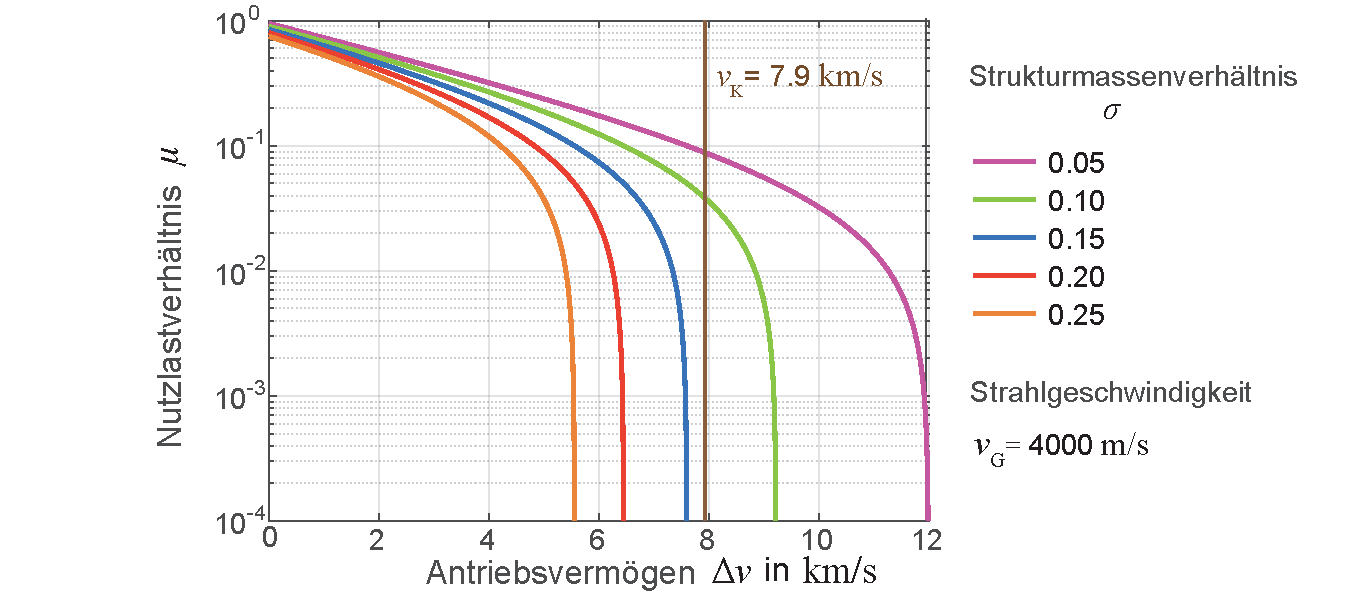
\includegraphics[width=\textwidth]{Rockets03.pdf} 
	\caption[Nutzlastverh�ltnis als Funktion der Endgeschwindigkeit $\Delta v$.]{Nutzlastverh�ltnis als Funktion der Endgeschwindigkeit $\Delta v$ bei angenommener Strahlgeschwindigkeit $v_\text{G} = \SI{4000}{\metre\per\second}$ nach Gleichung \eqref{eq:adyn_rockets13}. Die vertikale Linie zeigt die 1.~\gls{vkosmos}.}\index{Geschwindigkeit!1.~kosmische}
	\label{abb:adyn_rockets03}
\end{figure}

Zuvor aber noch eine Bemerkung zur charakteristischen Geschwindigkeit $\Delta v$. Im allgemeinen Fall wird man $\Delta v$ nur numerisch berechnen k�nnen, insbesondere bei l�nger andauernden Brennphasen des Triebwerks, wie wir das bei der numerischen Rechnung f�r \figref{adyn_rockets02} f�r den Aufstieg der Rakete im Gravitationsfeld der Erde getan haben. Wir hatten dort die anf�nglich noch stark wirkende Reibung der Atmosph�re unber�cksichtigt gelassen, werden dies aber sp�ter im \kap{adyn_launch_reentry} nachholen.\\
F�r die n�chsten Kapitel wollen wir den h�ufigen Fall eines zeitlich relativ kurzen Treibstoffaussto�es  voraussetzen. In diesem Fall k�nnen die wirkenden externen Kr�fte, insbesondere die Gravitationskraft $F_\text{G}$, als konstant angenommen werden und Gleichung \eqref{eq:adyn_rockets02} wird zu:
\begin{align}
     \Delta v &= - v_\text{G} \int_{m_0}^{m_\text{f}} \frac{\D m }{m} + F_\text{G} \int_{m_0}^{m_\text{f}} \frac{1}{\dot{m}} \frac{\D m}{m} = + \lk v_\text{G} - \frac{F_\text{G}}{\dot{m}_\text{T}} \rk\, \ln \frac{m_\text{f}}{m_0}		\,. \label{eq:adyn_rockets14}
\end{align}

\subsection{Prinzip der Stufenrakete}\label{kap:adyn_multistagerockets}

Wir haben im vorhergehenden Kapitel gesehen, dass mit einer einstufigen Rakete bei gegebenem Antriebsverm�gen die Nutzlast �u�erst begrenzt ist. Um gr��ere Nutzlasten ins Weltall zu bef�rdern, muss man das Prinzip der Stufenrakete \index{Stufenrakete} anwenden. Dieses besteht darin, dass w�hrend des Fluges unn�tig gewordene Strukturmassen der Rakete (leere Treibstoffbeh�lter, Triebwerke etc.) abgeworfen werden, um die verbleibende Antriebsenergie besser f�r die Beschleunigung der Nutzlasten zu verwenden. Man unterscheidet die Tandemstufung \index{Tandemstufung} (serielle Stufung) und die \index{Parallelstufung} Parallelstufung. Bei der ersteren erfolgt die Stufung �bereinander (\figref{adyn_rockets04}a), bei der Parallelstufung entsprechend parallel  (\figref{adyn_rockets04}b). H�ufig gibt es auch Mischformen \cite{Walter2018}. \\

\begin{figure}[H]
	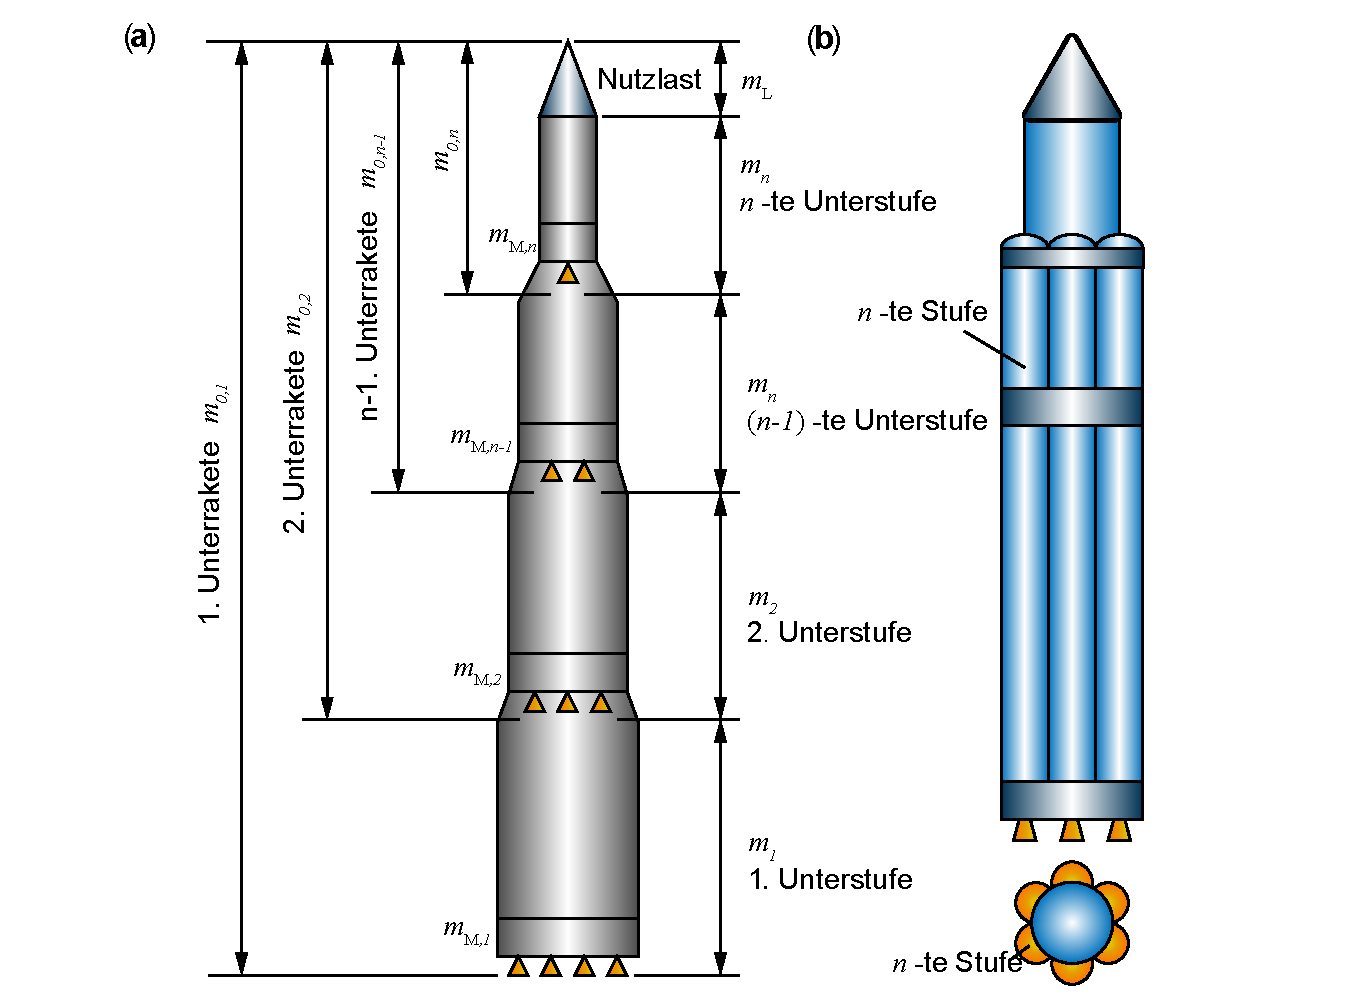
\includegraphics[width=\textwidth]{Mehrstufenraketen.pdf} 
	\caption[Mehrstufenprinzip bei Raketen.]{Mehrstufenprinzip bei Raketen. \fa Tandemstufung \fb Parallelstufung.}
	\label{abb:adyn_rockets04}
\end{figure}

Die Startmasse f�r eine $N$-stufige Rakete lautet:
\begin{align}
     m_0 &= \sum_{i=1}^N \, m_i + m_\text{L} \,, \label{eq:adyn_rockets15}
\end{align}
worin $m_\text{L}$ f�r die Nutzlast steht. Die Massen der einzelnen Stufen $m_i$ werden unterteilt in
\begin{align*}
     m_i &= m_{\text{T},i} + m_{\text{S},i}{} + m_{\text{M},i} \,.
\end{align*}
Hierin sind $m_{\text{T},i}$ die Massen des Treibstoffs, $ m_{\text{S},i}$ die Strukturmassen und $ m_{\text{M},i}$ die Triebwerksmassen der jeweils $i$-ten Stufe. Die Masse der Rakete nach Abbrennen und Abwerfen der $i$-ten Stufe ist gleichzeitig die Startmasse f�r die jeweilig n�chste Stufe, was die Definition von sogenannten Unterraketen mit den Massen $m_{0,i}$ erlaubt:
\begin{align}
\begin{split}
           m_{0,1} &= \lk \sum_{i=1}^N m_i \rk +  m_{\text{L}} = m_0 \,\\
		       m_{0,2} &= \lk \sum_{i=2}^N m_i \rk +  m_{\text{L}} \,\\
					         &\vdots \\
           m_{0,k} &= \lk \sum_{i=k}^N m_i \rk +  m_{\text{L}} \,\\
					         &\vdots \\
         m_{0,N+1} &= m_{\text{L}} = m_{\text{f}} \,.
\end{split} \label{eq:adyn_rockets16}
\end{align}


Mehrfache Anwendung der Raketen-Gleichung \eqref{eq:adyn_rocketequ} ergibt aus \eqref{eq:adyn_rockets16} f�r das Antriebsverm�gen\index{Antriebsverm�gen|textbf} $\Delta v$:
\begin{align}
     \Delta v &=  \sum_{i=1}^N v_{\text{G},i} \, \ln \frac{m_{0,i}}{m_{0,i}- m_{\text{T},i}} \,. \label{eq:adyn_rockets17}
\end{align}
Man beachte, dass im Nenner des Logarithmus von Gleichung \eqref{eq:adyn_rockets17} der Term $m_{0,i}- m_{\text{T},i}$ stehen muss, da zum Brenn-Endzeitpunkt der Stufe $i$ zwar der Treibstoff verbrannt ist, aber die Strukturen noch nicht abgeworfen worden sind. Man kann nun ein Strukturmassenverh�ltnis f�r die jeweiligen Stufen einf�hren:
\begin{align}
     \sigma_{\text{S},i} &= \frac{m_{0,i}- m_{\text{T},i} - m_{0,i+1}}{m_{0,i}} = \frac{m_{\text{M},i} + m_{\text{S},i}}{m_{0,i}}\,. \label{eq:adyn_rockets18}
\end{align}
Dieses kann man verstehen als das Verh�ltnis der momentanen (f�r $i$-te Stufe) eingesetzten Struktur- und Triebwerksmasse zur aktuellen Gesamtmasse, \dh der Masse der verbleibenden Unterrakete. Mit \eqref{eq:adyn_rockets18} folgt aus \eqref{eq:adyn_rockets17} f�r das gesamte Antriebsverm�gen:
\begin{align}
     \Delta v_\text{ges} &=  \sum_{i=1}^N v_{\text{G},i} \, \ln \frac{1}{\sigma_{\text{S},i} + m_{0,i+1}/m_{0,i}} = \sum_{i=1}^N v_{\text{G},i} \, \ln \frac{1}{\sigma_{\text{S},i} + \mu_{i+1}/\mu_i}  \,,\label{eq:adyn_rockets19}
\end{align}
wobei wir als 
\begin{align}
	\mu_i = m_{0,i}/m_0  \label{eq:adyn_rockets19a}
\end{align}
das Massenverh�ltnis der $i$-ten Unterrakete zur Gesamtstartmasse eingef�hrt haben, womit insbesondere gilt:
\begin{align}
		\mu_1 = 1\,,~~\mu_{N+1} = m_\text{L}/m_0 = \mu_\text{L}\,. \label{eq:adyn_rockets19b}
\end{align}
Wir sehen an Gleichung \eqref{eq:adyn_rockets19}, dass f�r das Antriebsverm�gen der Rakete die Struktur\-massen-Verh�ltnisse und die relativen Massenverh�ltnisse entscheidend sind. Man kann leicht �berpr�fen, dass \eqref{eq:adyn_rockets19} f�r $N=1$ in die Ziolkowski-Gleichung\index{Ziolkowski-Gleichung} �bergeht. Offensichtlich stellt \eqref{eq:adyn_rockets19} eine komplexe Optimierungsaufgabe f�r die Bestimmung des mehrstufigen Raketensystems bei vorgegebener Nutzlast $m_\text{L}$  und Maximierung \bzw Erreichung eines bestimmten Antriebsverm�gens $\Delta v_\text{ges}$ dar. 
Die Stufenoptimierungsaufgabe besteht insbesondere darin,  die Zahl der Stufen $N$ und die Massenaufteilung $m_{0,i}$ auf die einzelnen Raketenstufen so festzulegen, dass die Gesamtmasse  $m_0$ minimal wird. 
Vorgegeben sind dabei die Gasaustrittsgeschwindigkeiten $v_{\text{G},i}$ der einzelnen Stufen. Ebenso werden die Strukturmassenverh�ltnisse $\sigma_{\text{S},i}$ der einzelnen Stufen, die von der Beschleunigungsbelastung, der G�te der Konstruktion, der Bauweise und vielen anderen Faktoren abh�ngen, als bekannte Konstanten vorausgesetzt. Siehe dazu auch \probref{adyn_rocketbasic} und \probref{adyn_rocketopt2}, die Optimierungsaufgabe werden wir speziell in \probref{adyn_rocketopt1} durchf�hren.
In \figref{adyn_rockets05} haben wir das Nutzlastverh�ltnis und das Antriebsverm�gen mit den Werten der Saturn V und der Ariane 1 Raketen aufgetragen \cite{Messerschmid2017}. Man erkennt, dass mit h�herer Stufenzahl das Antriebsverm�gen wie erwartet zunimmt. 

\begin{figure}[H]
	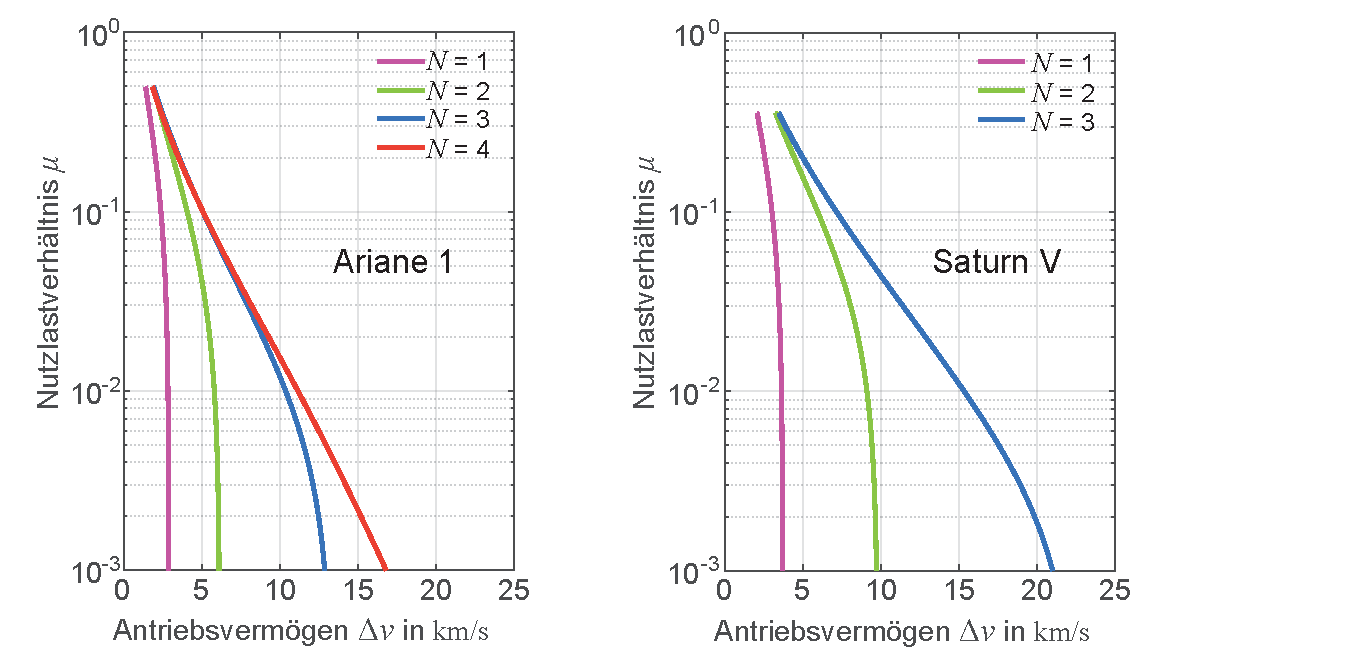
\includegraphics[width=\textwidth]{ArianeSaturn.pdf} 
	\caption[Nutzlastverh�ltnis f�r mehrstufige Raketen.]{Nutzlastverh�ltnis f�r mehrstufige Raketen (Werte f�r Saturn~V und der Ariane~1 siehe Tabelle \ref{tab:adyn_parameter_raketen} \cite{Messerschmid2017}).}
	\label{abb:adyn_rockets05}
\end{figure}





\clearpage
\section{Umlaufbahnen von k�nstlichen Himmelsk�rpern}\label{kap:adyn_orbits}

Im vorherigen Kapitel hatten wir die Geschwindigkeits�nderung eines Raumflugk�rpers unter Wirkung eines Schubs betrachtet. Wenn dieser Schub nur f�r kurze Zeit wirkt, k�nnen w�hrend dieser Phase dann alle anderen wirkenden Kr�fte und auch die Positions�nderung des Raumschiffs \bzw der Rakete unber�cksichtigt bleiben und man muss nur die Geschwindigkeits�nderung $\Delta v$ betrachten. Wirkt der Schub hingegen �ber eine l�ngere Zeit, dann muss man die Bewegungsgleichung \eqref{eq:adyn_rockets01} unter Ber�cksichtigung aller wirkenden Kr�fte entsprechend integrieren (wie zum Beispiel in der Rechnung zu \figref{adyn_rockets02}). 
Im Folgenden nehmen wir die Wechselwirkungszeit des Schubs zun�chst als sehr kurz an, in \kap{adyn_kont_maneuver} werden wir auch Phasen betrachten, in denen der Schub �ber eine l�ngere Zeit wirkt.\\
In den Flugphasen ohne Schub bewegt sich das Raumschiff im Gravitationsfeld der Himmelsk�rper nach den Gesetzen der Himmelsmechanik, im einfachsten Fall auf Kepler-Bahnen des Zweik�rpersystems Himmelsk�rper-k�nstlicher Satellit. Wir wollen daher zun�chst den Fall von Satellitenbahnen um die Erde betrachten und stellen daf�r noch einmal die im Kapitel der Himmelsmechanik (Kap. \ref{chap:hm}) hergeleiteten wichtigsten Beziehungen f�r das Zweik�rperproblem, angepasst f�r (geschlossene) Satellitenbahnen um die Erde, zusammen.

\subsection{Grundlegende Beziehungen aus der Himmelsmechanik f�r Satellitenbahnen um die Erde}\label{kap:adyn_recap_hm}

F�r k�nstliche Satelliten der Masse $m$ um die Erde gilt: 
\begin{align}
    m \ll m_\text{E} ~~~~ \rightarrow ~~~~ \mu_\text{G} = G\,m_\text{E}\,.  \label{eq:adyn_orbit01}
\end{align}
Aus den im \kap{hm_abl_kepler} hergeleiteten Beziehungen f�r die Ellipsenbahn folgt dann mit dem Drehimpuls $L$ f�r die Bahnparameter $p, a, e ~\text{und}~ T_\text{P}$ und den Koordinaten $r, v$:
\begin{subequations}
\begin{align}
    r &= \frac{p}{1+\e \cos\upsilon} ~~~\text{mit}\\
    p &=\frac{L^2}{G\,m_\text{E}}\,,~~~ e = \sqrt{1-\frac{L^2}{a\,m_\text{E}}}~~~\text{und}~~~ a= \sqrt[3]{\frac{G\,m_\text{E}\,T_\text{P}{}^2}{4\pi^2}}\,.
		\label{eq:adyn_orbit01a} 
\end{align}
\end{subequations}
F�r das \gls{perigee}\index{Perig�um|textbf} \bzw das \gls{apogee}\index{Apog�um|textbf} gilt dann: 
\begin{align}
    r_\text{min} &= r_\text{per} = \frac{p}{1+e} ~~~ \text{und}~~~  r_\text{max} = r_\text{apo} = \frac{p}{1-e} \,. \label{eq:adyn_orbit01b} 
\end{align}

\begin{figure}[H]
	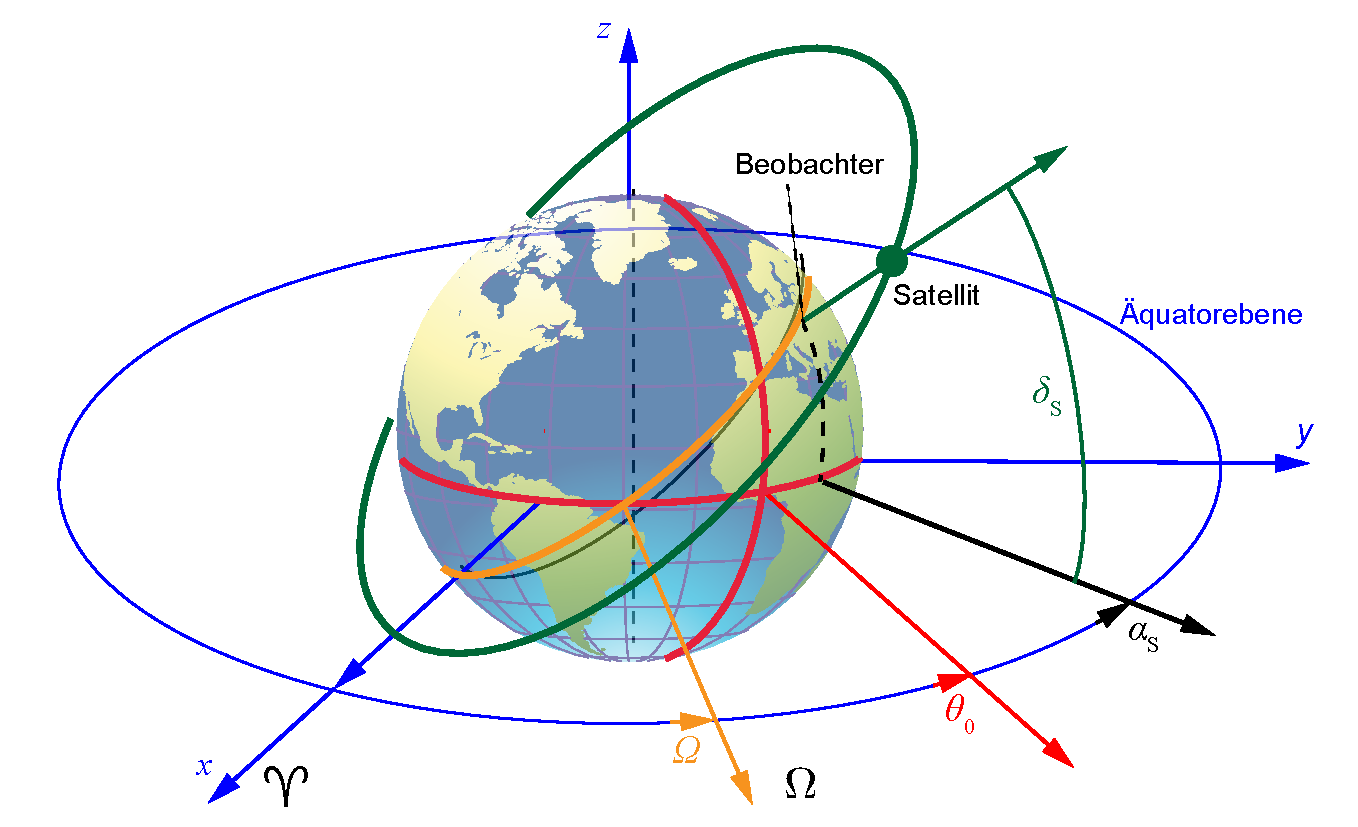
\includegraphics[width=\textwidth]{Orbits01.pdf} 
	\caption[Bahnparameter und Koordinatensystem einer Satellitenbahn um die Erde.]{Bahnparameter und Koordinatensystem einer Satellitenbahn um die Erde. Die Winkel $\Omega,\, \theta_0,\, \alpha_\text{S}$ werden jeweils vom Fr�hlingspunkt\index{Fr�hlingspunkt} aus gemessen.}
	\label{abb:adyn_orbits01}
\end{figure}

Die \gls{visvivaadyn} \eqref{eq:hm_vis-viva} lautet
\begin{align}
    v^2 = G\,m_\text{E} \lk \frac{2}{r} -\frac{1}{a}\rk \,, \label{eq:adyn_orbit03}
\end{align}
woraus sich die Geschwindigkeiten am Perig�um \bzw Apog�um ergeben:
\begin{subequations}
\begin{align}
    v_\text{max} &= v (r_\text{min}) = v_\text{per} = \sqrt{\frac{G\,m_\text{E}}{a}}\,\sqrt{\frac{1+\e}{1-\e}} ~~~ \text{\bzw} \\
		v_\text{min} &= v (r_\text{max}) = v_\text{apo} = \sqrt{\frac{G\,m_\text{E}}{a}}\,\sqrt{\frac{1-\e}{1+\e}}\,.
\end{align} \label{eq:adyn_orbit04}
\end{subequations}

Die Bahnparameter $\Omega,\omega,i$ (\figref{adyn_orbits01}) entsprechen den Bahnparametern, wie sie f�r Planeten und andere nat�rliche Himmelsk�rper in \kap{hm_bewegungsgl} hergeleitet (\figref{hm_bahnelemente}) wurden. \\
Entsprechend kann man die Bewegung eines k�nstlichen Satelliten au�erhalb der Schubphasen durch die in \kap{hm_bahnen_hk_ss} hergeleiteten Gau�schen
%\footnote{Johann Carl Friedrich Gau� (auch oft Gauss) (1777 -- 1855) war ein deutscher Mathematiker, Astronom, Geod�t und Physiker. Wegen seiner �berragenden wissenschaftlichen Leistungen galt er bereits zu seinen Lebzeiten als \textit{Princeps mathematicorum - F�rst der Mathematiker}. Seine Arbeiten erstreckten sich von vielen Feldern der Mathematik und Physik auch auf angewandte Gebiete, zum Beispiel der Landesvermessung und der elektromagnetischen Telegrafie.}\indexp{Gau�, Johann Carl Friedrich} 
 Vektoren\footnote{In \kap{hm_bahnen_hk_ss} hatten wir der historischen Konvention folgend die Gau�schen Vektoren mit $\vec{P}\vec{Q}\vec{R}$  bezeichnet. Um Verwechslungen mit dem Radiusvektor $\vec{R}$ zu vermeiden, schreiben wir ab hier $\vec{R}=\vec{W}$.}  \eqref{eq:hm_gauss_ansatz},\eqref{eq:hm_gauss_vektoren} $\vec{P}\vec{Q}\vec{W}$ beschreiben:
\begin{align}
\begin{split}
    \vec{r}_\text{S} &= 
    \begin{pmatrix}
        x_\text{S} \\
        y_\text{S} \\
        z_\text{S}
    \end{pmatrix}
    = \mathbb{U}\,r\,    
		\begin{pmatrix}
        \cos\upsilon \\
        \sin\upsilon \\
        0
    \end{pmatrix}
		= 
    \lk \vec{P}\vec{Q}\vec{W}\rk\,\,r\,
    \begin{pmatrix}
        \cos\upsilon \\
        \sin\upsilon \\
        0
    \end{pmatrix} \\
    &= \mathbb{R}_z\lk -\Omega\rk\,\mathbb{R}_x\lk -i\rk\,\mathbb{R}_z\lk -\omega\rk\,\,r\,
    \begin{pmatrix}
        \cos\upsilon \\
        \sin\upsilon \\
        0
    \end{pmatrix} \,,
\end{split} \label{eq:adyn_orbit05}
\end{align}\\
wobei sich die wahre Anomalie\index{Anomalie!wahre} $\upsilon$ aus der Kepler-Gleichung \eqref{eq:hm_keplerglg} �ber die exzentrische Anomalie $E$\index{Anomalie!exzentrische} berechnen l�sst.
Wie man aus \figref{adyn_orbits01} sieht, ist die Satellitenbahnebene ein Gro�kreis, der eindeutig durch die Bahnneigung (Inklination) $i$ und den aufsteigenden Knoten festgelegt ist. Dieser Gro�kreis schneidet somit die �quatorebene unter dem Winkel~$i$. Die maximale (minimale) geographische Breite, unter der der Satellit beobachtet werden kann, ist dann durch $+\,i$ \bzw $-\,i$ gegeben, wie man ebenfalls aus \figref{adyn_orbits01} sieht.

\subsection{Bestimmung der Bodenspuren k�nstlicher Satelliten} \label{kap:adyn_orbits_groundtracks}

Wir nehmen zun�chst an, dass uns die Bahnparameter des Satelliten bekannt sind, wir also seine geozentrische Bahn berechnen k�nnen, so wie wir das f�r Planeten als nat�rliche Satelliten der Sonne im \kap{hm_bahnen_hk_ss} ausf�hrlich beschrieben haben. Wir wollen jetzt aber auch die Projektion dieser Bahn auf die Erdoberfl�che berechnen. Dazu brauchen wir zu jeder Zeit den geographischen Ort, �ber dem der Satellit senkrecht steht. Die jeweilige geographische Breite $\varphi_\text{B}$ des Ortes B (eigentlich die geozentrische Breite), �ber welchem der Satellit im Zenit steht, ist durch die Deklination des Satelliten $\delta_\text{S}(t)$ gegeben, die sich wiederum aus \eqref{eq:adyn_orbit05} berechnen l�sst. Die entsprechende geographische L�nge $\lambda_\text{B}$ h�ngt, wie im \kap{hm_zeitdefinition}, \figref{hm_Sternzeit_Stundenwinkel} gezeigt, von der Rektaszension $\alpha_\text{S}\lk t\rk$ des Satelliten ab (vgl. \eqref{eq:hm_std_winkel_tau}), woraus sich mit \eqref{eq:hm_UT_3} die folgende Beziehung ergibt \cite{Montenbruck2012}:
\begin{align}
    \lambda_\text{B}\lk t\rk = \alpha_\text{S}\lk t\rk -\theta_0 = \alpha_\text{S}\lk t\rk + 280.4606\degree + 360.9856473\degree d \,. \label{eq:adyn_orbit06}
\end{align}
Hierin ist $\theta_0$ die (mittlere) Greenwich Sternzeit (GMST) und $d$ ist die seit dem $1.1.2000$ verstrichene Zeit in (Julianischen) Tagen, die sich einfach aus $d = \mathrm{MJD} - 51544.5$ berechnen l�sst. Sinnvollerweise benutzt man das (modifizierte) Julianische Datum MJD ebenfalls zur Berechnung von $\alpha_\text{S}(t)$ und $\delta_\text{S}(t)$ (\vgl \kap{hm_zeitdefinition}). Als Ergebnis der �ber die Beziehung \eqref{eq:adyn_orbit06} ber�cksichtigten Erdrotation relativ zur Bewegung des Satelliten ist der Pfad des Satelliten auf der Erdoberfl�che kein einfacher Gro�kreis mehr, sondern hat \zb f�r einen sogenannten \gls{LEO}\index{Low Earth Orbit, LEO} die in \figref{adyn_orbits02} dargestellte Form. Offensichtlich sind die Bodenspuren f�r aufeinanderfolgende Orbits wegen der Erdrotation jeweils westlich verschoben.
F�r einen Satelliten mit einer ann�hernd kreisf�rmigen Bahn und einer Umlaufzeit von $T_\text{p}$ in Minuten verschiebt sich die geographische L�nge eines Beobachtungspunktes auf dem �quator um 
\begin{align*}
    \Delta \lambda_\text{B,�q} = -\dot{\theta}_0\,T_\text{p} = -0.2507\degree\,T_\text{p}
\end{align*}
pro Umlauf (\figref{adyn_orbits02}). \\
F�r andere Satellitenbahnen, wie \zb geostation�re Bahnen (\gls{GEO}, GEO)\index{Orbit!geostation�rer, GEO} oder hoch elliptische Bahnen (\gls{HEO}, HEO)\index{Orbit!highly elliptical, HEO} ergeben sich deutlich andere Bodenspuren (siehe \figref{adyn_orbits03} und \probref{adyn_orbits2}).

\begin{figure}[H]
	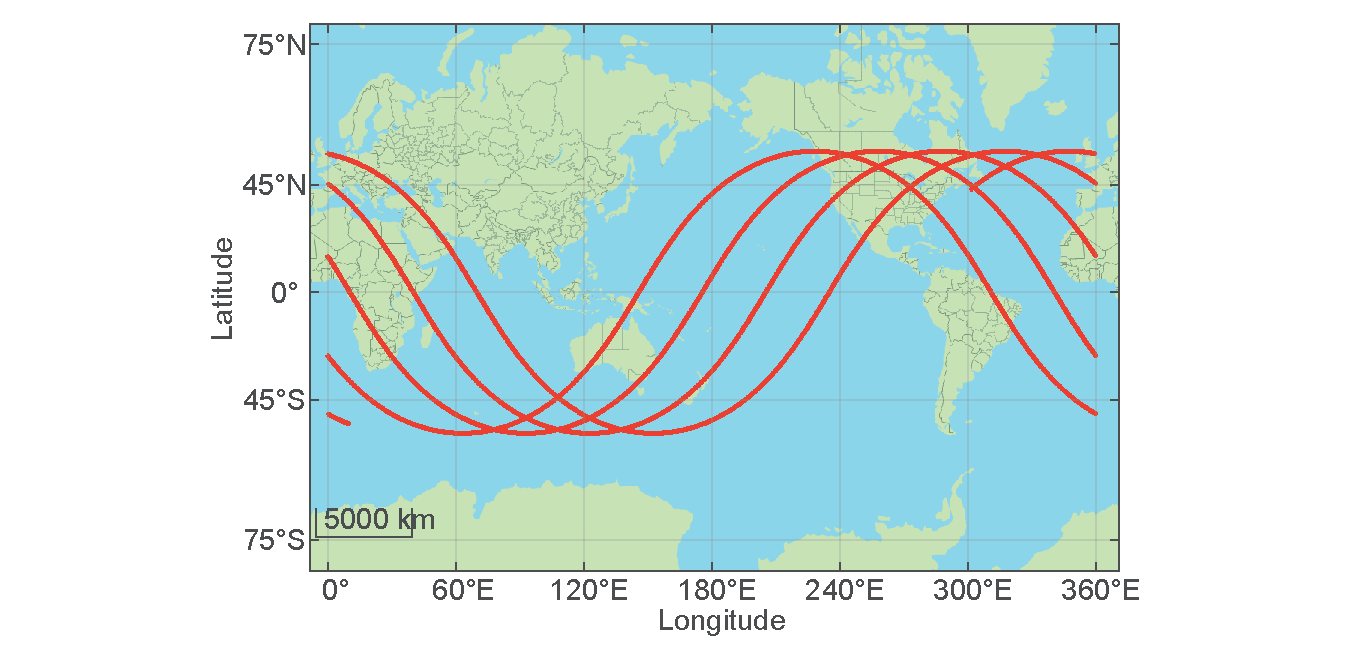
\includegraphics[width=\textwidth]{Orbits02.pdf} 
	\caption[Bodenspur eines LEO-Satelliten.]{Bodenspur eines LEO-Satelliten. $a = \SI{8000}{\km},\; e = 0.0,\; i = 55\degree$.}
	\label{abb:adyn_orbits02}
\end{figure}

\begin{figure}[H]
	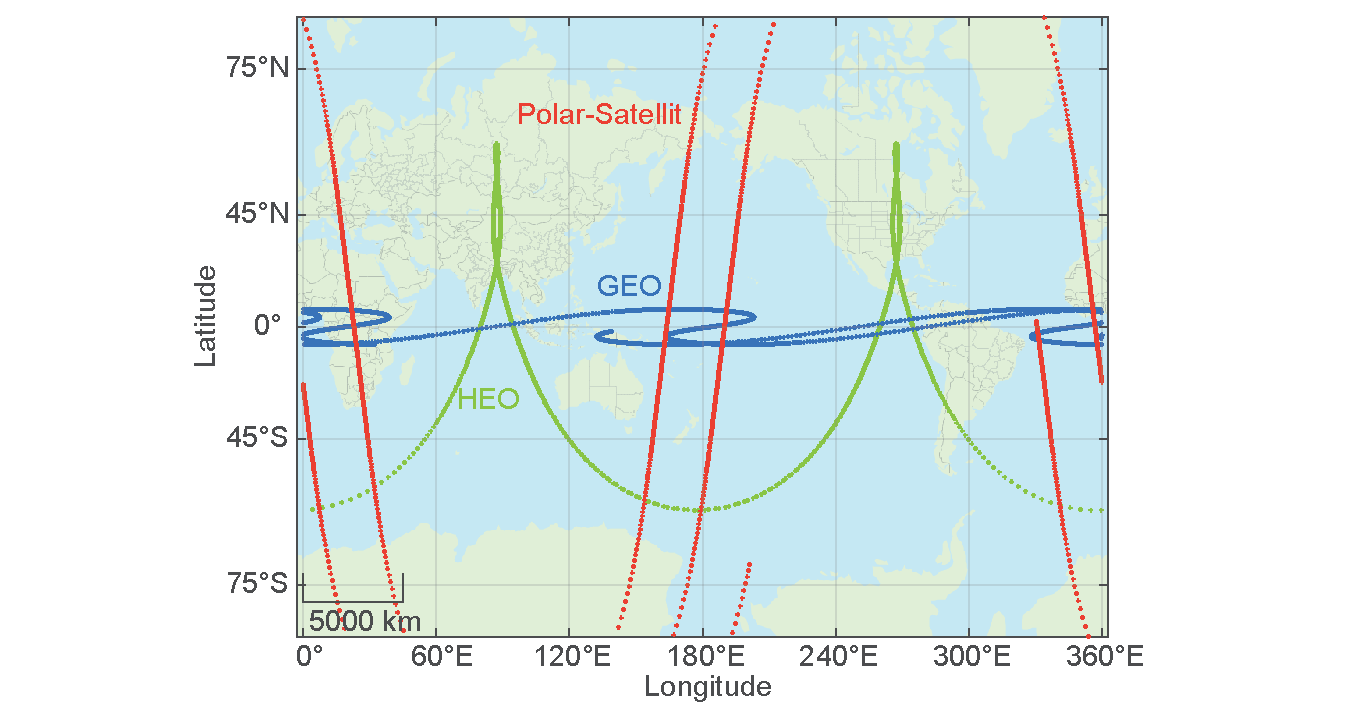
\includegraphics[width=0.9\textwidth]{Orbits03a.pdf} 
	\caption[Bodenspuren von verschiedenen Satelliten.]{Bodenspuren von verschiedenen Satelliten. GEO-artiger Satellit:\, $a = \SI{25000}{\km},\, e = 0.73,\, i = 8\degree,\, \Omega =45\degree$,\,\, HEO (Typ Molnija-Satelliten):\, $a = \SI{26555}{\km},\, e = 0.72,\, i = 63.4\degree,\, \Omega =120\degree,\,\omega =270\degree$,\,\, Polar-Satellit:\, $a = \SI{7330}{\km},\, e = 0.0,\, i = 93\degree,\, \Omega =130\degree,\,\omega =0\degree$. Siehe auch \mscr~ \mladynref{SatPositionen01.m}.}
	\label{abb:adyn_orbits03}
\end{figure}

\subsection{Topographische Beziehungen f�r die Beobachtungen k�nstlicher Satelliten} \label{kap:adyn_orbits_topo}

Will man die Beobachtungsdaten eines in der Erdumlaufbahn befindlichen Satelliten f�r eine bestimmte Bodenstation aus den Bahnparametern berechnen, so muss man, wie bereits im Kapitel Himmelsmechanik (\kap{hm_koordinatensysteme}) gezeigt, in ein topozentrisches Koordinatensystem wechseln, da ein Beobachter auf der Erdoberfl�che einen Satelliten aus der Horizont\-ebene (\figref{adyn_satobserv01}) beobachten wird. Die Bodenspuren (englisch \textit{Ground-Tracks}) aus dem vorherigen Kapitel geben eine gewisse Indikation, aber man erh�lt daraus keine Aussage �ber die H�he des Satelliten, die Sichtbarkeitsdauer und auch die Beobachtungsrichtung. Um diese Gr��en zu berechnen, gehen wir in ein lokales tangentiales Koordinatensystem, welches ein spezielles topozentrisches \KOS\ darstellt (\figref{adyn_satobserv01}, \vgl auch \kap{hm_koordinatensysteme}). Wir wollen nun die Position des Satelliten in diesem Koordinatensystem ausdr�cken. \\

\begin{figure}[H]
	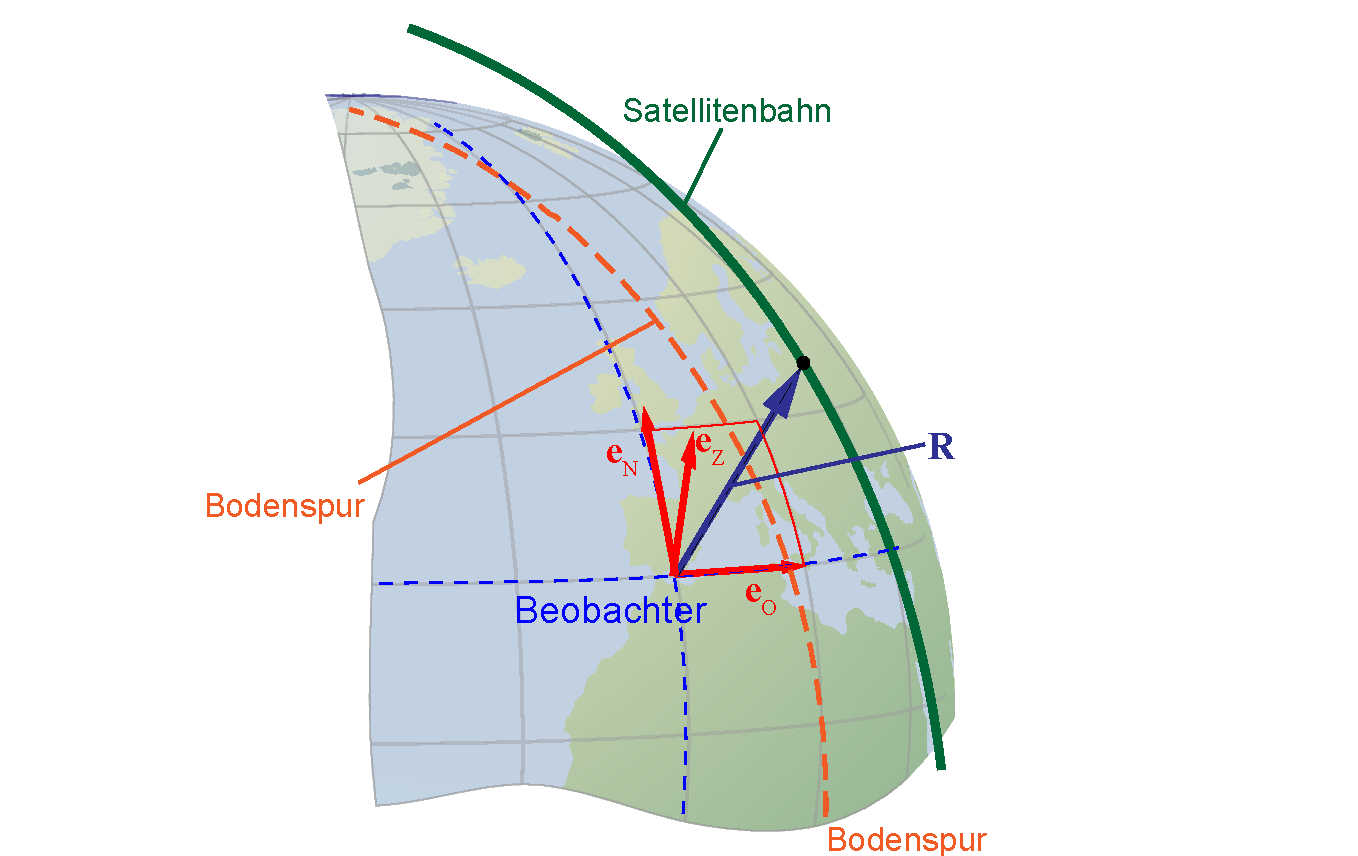
\includegraphics[width=\textwidth]{SatObserver01.pdf} 
	\caption[Horizontkoordinatensystem.]{Horizontkoordinatensystem und beobachtbarer Anteil der Umlaufbahn eines Satelliten.}
	\label{abb:adyn_satobserv01}
\end{figure}

Wir starten mit den Koordinaten des Satelliten $\vec{r}$ im geozentrisch-�quatorialen Koordinatensystem und schreiben diese als $\vec{r}_\text{S}$ in ein erdfestes geozentrisch-�quatorialen System  um, in dem wir die Rotation der Erde durch den Stundenwinkel von Greenwich $\theta$ ber�cksichtigen (vgl. \kap{hm_koordinatensysteme}, Gleichung \eqref{eq:hm_LMST}, \figref{hm_Sternzeit_Stundenwinkel}):
\begin{align}
\begin{split}
    \vec{r}_\text{S} &= \mathbb{R}_\text{z}\!\lk\theta\rk\,\vec{r}\, ~~~~
\text{mit} ~~~~ \mathbb{R}_\text{z}\lk\theta\rk = 
    \begin{pmatrix}
         \cos\theta & ~~\sin\theta & ~~0 \\
        -\sin\theta & ~~\cos\theta & ~~0 \\
        0             & ~~0            &~~ 1
    \end{pmatrix} \\
		\text{und}~~~~\theta &= 280.4606\degree + 360.9856473\degree \cdot \lk \mathrm{MJD} - 51544.5\rk \,,
\end{split} \label{eq:adyn_statobserv01} 
\end{align}
worin MJD das modifizierte Julianischem Datum (Kap. \ref{kap:hm_zeitdefinition}) des Beobachtungszeitpunkts ist. Die Koordinaten des Beobachters sind gegeben durch:
\begin{align}
    \vec{r}_\text{B} = R_\text{E}
    \begin{pmatrix}
		                     \cos \varphi_\text{B} \, \cos \lambda_\text{B} \\
		                     \cos \varphi_\text{B} \, \sin \lambda_\text{B} \\
		                     \sin \varphi_\text{B}
    \end{pmatrix} \,, \label{eq:adyn_statobserv02}
\end{align} 
wobei wir f�r die geographische Breite \bzw L�nge verk�rzend $\varphi=\varphi_\text{B}$ \bzw $\lambda= \lambda_\text{B}$ schreiben.\footnote{Wie bereits erw�hnt, setzen wir die geographische Breite hier gleich der geozentrischen Breite, \dh wir vernachl�ssigen die Abplattung der Erde.} Der topozentrische, fest mit der Erde verbundene Koordinatenvektor $\vec{R}_\text{S}$ ist in �quatorialen Koordinaten dann durch 
\begin{align}
\begin{split}
    \vec{R}_\text{S} &= \vec{r}_\text{S} - \vec{r}_\text{B}\,
\end{split} \label{eq:adyn_statobserv03} 
\end{align}
bestimmt.\\
Die Einheitsvektoren des topozentrischen \KOS\ lauten:
\begin{align}
\begin{split}
    \vec{e}_\text{O} &= 
    \begin{pmatrix}
        -\sin\lambda_\text{B}\\
        +\cos\lambda_\text{B}\\
        0
    \end{pmatrix} ~~~ \text{(Ost-Richtung)}\,,~~~
    \vec{e}_\text{N} = 
    \begin{pmatrix}
        -\sin\varphi_\text{B}\cos\lambda_\text{B}\\
        -\sin\varphi_\text{B}\sin\lambda_\text{B}\\
        \cos\varphi_\text{B}
    \end{pmatrix} ~~~ \text{(Nord-Richtung)}\,,\\
    \vec{e}_\text{Z} &= 
    \begin{pmatrix}
        \cos\varphi_\text{B}\cos\lambda_\text{B}\\
        \cos\varphi_\text{B}\sin\lambda_\text{B}\\
        \sin\varphi_\text{B}
    \end{pmatrix} ~~~ \text{(Zenit-Richtung)}\,.
\end{split} \label{eq:adyn_statobserv04} 
\end{align}
F�r die Umrechnung von erdfesten �quatorialen in topozentrische Koordinaten verwendet man die Transformationsmatrix $\mathbb{U}$, die durch die drei Einheitsvektoren nach \eqref{eq:adyn_statobserv04}  definiert wird:
\begin{align}
    \mathbb{U}= 
		\begin{pmatrix}
        \vec{e}_\text{O}{}^\text{T} \\
        \vec{e}_\text{N}{}^\text{T} \\
        \vec{e}_\text{Z}{}^\text{T} 
    \end{pmatrix} =
    \begin{pmatrix}
        -\sin\lambda_\text{B} &~~ +\cos\lambda_\text{B} &~~ 0 \\
        -\sin\varphi_\text{B}\,\cos\lambda_\text{B} &~~ -\sin\varphi_\text{B}\,\sin\lambda_\text{B}&~~\cos\varphi_\text{B}\\
        +\cos\varphi_\text{B}\,\cos\lambda_\text{B} &~~ +\cos\varphi_\text{B}\,\sin\lambda_\text{B}&~~ \sin\varphi_\text{B}
    \end{pmatrix} \,. \label{eq:adyn_statobserv05} 
\end{align}
Wir erhalten damit leicht den Beobachtungsvektor zum Satelliten $\vec{R}$ in kartesischen topozentrischen Koordinaten:% (Distanz $R$, Azimut $\mathcal{A}$ und H�he $h$)
\begin{align}
    \vec{R} = 
    \begin{pmatrix}
        R_\text{O} \\
        R_\text{N}\\
        R_\text{Z}
    \end{pmatrix}
    &= \mathbb{U}\,\vec{R}_\text{S} =
    \mathbb{U}\,\lek \lk \mathbb{R}_\text{z}\lk \theta\rk \,\vec{r} \rk - \vec{r}_\text{B} \rek \,.
\end{align} \label{eq:adyn_statobserv06}
Die Beobachtungsdaten Azimut $\mathcal{A}$ und H�he $h$ sind dann leicht zu bestimmen:
\begin{align}
    \mathcal{A} &= \arctan\lk \frac{R_\text{O}}{R_\text{N}}\rk ~~~\text{und}~~~
    h = \arctan\lk \frac{R_\text{Z}}{\sqrt{R_\text{O}{}^2 + R_\text{N}{}^2}}\rk \,.\label{eq:adyn_statobserv07}
\end{align}
Wie aus \figref{adyn_satobserv01} ableitbar, beschreibt $\mathcal{A}$ den Winkel zwischen der Bodenspur des Satelliten und der Nordrichtung und $h$ den Winkel zwischen der Richtung von Beobachter zum Satelliten und der Horizontebene. In \probref{adyn_orbits3} werden wir die Beobachtungsdaten f�r einen polaren Satelliten und die ISS berechnen. %�bung7

\subsection{Bestimmung der Bahn k�nstlicher Satelliten vom Boden aus} \label{kap:adyn_orbits_determination}

\subsubsection{Bestimmung der Bahn k�nstlicher Satelliten aus Orts- und Geschwindigkeitsmessungen vom Boden} \label{kap:adyn_orbits_determination_rv}

Wir nehmen an, dass zu einem Zeitpunkt $t$ die geozentrischen Orts- \bzw Geschwindigkeitsvektoren ($\vec{r}, \vec{v}=\dot{\vec{r}}$) des Satelliten gegeben sind.\\
Der spezifische Drehimpuls $\vec{L} = \vec{r} \times \dot{\vec{r}} = \begin{pmatrix}
    y\,\dot{z} - z\,\dot{y}\\
    z\,\dot{x} - x\,\dot{z}\\
    x\,\dot{y} - y\,\dot{x}
\end{pmatrix}$ ist mit dem Gau�-Vektor\index{Gau�-Vektor|textbf} $\vec{W}$ wie folgt verkn�pft:
\begin{align}
    \begin{pmatrix}
        \sin i \,\sin\Omega\\
        \sin i \,\cos\Omega\\
        \cos i
    \end{pmatrix}
    = 
    \begin{pmatrix}
        +L_x/L\\
        -L_y/L\\
        +L_z/L
    \end{pmatrix}
    = 
    \begin{pmatrix}
        +W_x\\
        -W_y\\
        +W_z
    \end{pmatrix} \,. \label{eq:adyn_Bahnpara01}
\end{align}
Daraus erh�lt man sofort
\begin{align}
    i = \arctan\lk\frac{\sqrt{W_x{}^2+W_y{}^2}}{W_z}\rk \label{eq:adyn_Bahnpara02}
\end{align}
und 
\begin{align}
    \Omega = \arctan\lk\frac{W_x}{-W_y}\rk \label{eq:adyn_Bahnpara03}\,.
\end{align}
Der Drehimpuls ist nach \eqref{eq:hm_kegelschnitt} \bzw  \eqref{eq:adyn_orbit01a} mit dem Parameter $p$ �ber 
\begin{align}
    p = \frac{L^2}{G\,m_\text{E}} \label{eq:adyn_Bahnpara04}
\end{align}
verkn�pft. Der \textit{vis-viva-Satz}\index{vis-viva-Satz} \eqref{eq:hm_vis-viva} \bzw \eqref{eq:adyn_orbit03} ergibt aus den Messwerten sofort die gro�e Halbachse $a$ und die mittlere Bewegung\index{Bewegung!mittlere} $n$ �ber:
\begin{align}
    a = \lk \frac{2}{r} - \frac{v^2}{G\,m_\text{E}} \rk^{-1}~~~\text{\bzw}~~~ n = \sqrt{\frac{G\,m_\text{E}}{a^3}} \,, \label{eq:adyn_Bahnpara05}
\end{align}
und damit erhalten wir auch die Exzentrizit�t $e$: 
\begin{align}
    e = \sqrt{1-\frac{p}{a}} \,.\label{eq:adyn_Bahnpara07}
\end{align}
�ber die exzentrische Anomalie 
\begin{align}
    E\lk t\rk = \arctan\lk\frac{\vec{r}\cdot\vec{v}/(a^2\,n)}{1-r/a}\rk \label{eq:adyn_Bahnpara08}
\end{align}
und die Kepler-Gleichung erh�lt man die mittlere Anomalie zum Zeitpunkt $t$:
\begin{align}
    M\lk t\rk =E\lk t \rk - e\,\sin E\lk t\rk \label{eq:adyn_Bahnpara09}\,.
\end{align}
Etwas aufwendiger ist die Berechnung des Arguments des Perig�ums. \\
Man muss zun�chst die L�nge $u$ berechnen,
\begin{align}
    u = \arctan\lk\frac{z/\sin i }{x\,\cos\Omega +y\,\sin\Omega}\rk\,. \label{eq:adyn_Bahnpara10}
\end{align}
Die mittlere Anomalie $\upsilon$ kann dann aus der exzentrischen Anomalie $E$ \eqref{eq:adyn_Bahnpara08} �ber 
\begin{align}
    \upsilon = \arctan\lk \frac{\sqrt{1-e^2}\,\sin E}{\cos E-e}\rk \label{eq:adyn_Bahnpara11}
\end{align}
berechnet werden. Schlie�lich erh�lt man �ber 
\begin{align}
   \omega = u-\upsilon  \label{eq:adyn_Bahnpara12}
\end{align}
das letzte noch fehlende Bahnelement.
Wir verweisen auf eine Anwendung der gerade beschriebenen Vorgehensweise in \probref{adyn_orbits1}. %�bung5

\subsubsection{Bestimmung Bahnparameter bei kreisf�rmigen und �quatorialen Bahnen}  \label{kap:adyn_orbits_determination_singulaer}

Die Bestimmung der Bahn (Ort, Geschwindigkeit) eines Satelliten aus den Bahnelementen stellt keine besondere Schwierigkeit dar, selbst wenn die Exzentrizit�t und die Inklination ungef�hr Null sind, \dh $e\approx 0$ und $i\approx 0$.\\
Das inverse Problem, die Bahnparameter aus Einzelbeobachtungen von Satelliten mit nahezu kreisf�rmigen Bahnen oder Bahnen in der �quatorebene zu bestimmen, ist nicht so trivial. Das Argument des Perig�ums $\omega$ ist f�r kreisf�rmige Bahnen unbestimmt und kleine �nderungen der Beobachtungsdaten oder numerische Fehler f�hren zu gro�en �nderungen des Wertes f�r $\omega$. Analoges gilt f�r die Inklination $i$ bei geostation�ren Bahnen. Daher hat man f�r solche F�lle einen alternativen Satz von Bahnparametern konstruiert: 
\begin{align}
\begin{split}
     a&= a\,,~~~~\lambda=\Omega+\omega+M\,,\\
		 h&= e\,\sin\lk\Omega+\omega\rk\,,~~~~\eta  = \tan\frac{i}{2}\,\sin\Omega\,,\\
	  ~k&= e\,\cos\lk\Omega+\omega\rk\,,~~~\kappa = \tan\frac{i}{2}\,\cos\Omega\,. 
\end{split} \label{eq:adyn_bahnbest_01}
\end{align}
Hierin sind $M$ die mittlere Anomalie, die durch die Umlaufzeit bestimmt ist, und $\lambda$ die mittlere L�nge des Satelliten, die auch als ungef�hre Rektaszension des Satelliten auf der kreisf�rmigen Bahn interpretiert werden kann.\\
Man definiert nun ein neues $(\vec{f},\,\vec{g})$-Koordinatensystem, das aus den Gau�-Vektoren\index{Gau�-Vektor} $\vec{P}$,\,$\vec{Q}$ durch Drehung um den Winkel $\Omega+\omega$ hervorgeht:
\begin{subequations}
\begin{align}
    \vec{f} &= \cos\lk\omega+\Omega\rk\,\vec{P} - \sin\lk \omega+\Omega\rk\,\vec{Q} = \frac{1}{1+\eta^2+\kappa^2}
    \begin{pmatrix}
        1-\eta^2+\kappa^2\\
        2\eta\kappa\\
        -2\eta
    \end{pmatrix}\,,\label{eq:adyn_bahnbest_02a}\\
    \vec{g} &= \sin\lk\omega+\Omega\rk\,\vec{P} +\cos\lk \omega+\Omega\rk\,\vec{Q} = \frac{1}{1+\eta^2+\kappa^2}
    \begin{pmatrix}
        2\eta\kappa\\
        1+\eta^2-\kappa^2\\
        2\kappa
    \end{pmatrix}\,. \label{eq:adyn_bahnbest_02b}
\end{align}
\end{subequations}
Der Ortsvektor der Bahn ist in diesem \KOS\ dann gegeben durch 
\begin{subequations}
\begin{align}
    \vec{r} &= X\,\vec{f} +Y\,\vec{g}\label{eq:adyn_bahnbest_03a}\,,\\
    X &= a\lek \lk 1-h^2\,\beta\rk\,\cos\lk \Lambda\rk + h\,k\,\beta\,\sin\lk \Lambda\rk-k\rek \label{eq:adyn_bahnbest_03b}\,, \\
    Y &= a\lek\lk 1-k^2\,\beta\rk\,\sin\lk \Lambda\rk + h\,k\,\beta\,\cos\lk \Lambda\rk -h\rek \label{eq:adyn_bahnbest_03c}
\end{align}
\end{subequations}
mit
\begin{align}
    \beta = \frac{1}{1+\sqrt{1-h^2-k^2}}\label{eq:adyn_bahnbest_04}
\end{align}
und der exzentrischen L�nge
\begin{align}
    \Lambda = E+\omega+\Omega\,.\label{eq:adyn_bahnbest_05}
\end{align}
Analog ergibt sich f�r den Geschwindigkeitsvektor
\begin{subequations}
\begin{align}
    \dot{\vec{r}} &= \dot{X}\,\vec{f} +\dot{Y}\,\vec{g}\,, \label{eq:adyn_bahnbest_06a}\\
    \dot{X} &= \frac{a^2\,n}{r}\,\lk h\,k\,\beta\,\cos\lk \Lambda\rk -\lk 1-h^2\,\beta\rk\,\sin\lk \Lambda\rk\rk\,, \label{eq:adyn_bahnbest_06b} \\
    \dot{Y} &= \frac{a^2\,n}{r}\,\lk -h\,k\,\beta\,\sin\lk \Lambda\rk -\lk 1-k^2\,\beta\rk\,\cos\lk \Lambda\rk\rk\,. \label{eq:adyn_bahnbest_06c}
\end{align}
\end{subequations}
Die exzentrische L�nge $\Lambda$ ersetzt die exzentrische Anomalie $E$ und bestimmt sich aus:
\begin{align}
    \Lambda-k\,\sin\lk \Lambda\rk +h\,\cos\lk \Lambda\rk = \lambda = M+\omega+\Omega\,,\label{eq:adyn_bahnbest_07}
\end{align}
w�hrend sich der Betrag des Abstandsvektor $r$ durch 
\begin{align}
    r = a\,\lk 1-k\,\cos\lk \Lambda\rk -h\,\sin\lk \Lambda\rk\rk \label{eq:adyn_bahnbest_08}
\end{align}
ausdr�cken l�sst. \\
Wir halten nochmals fest, dass als Messwerte die kartesischen Koordinaten
\begin{equation*}
  \vec{r}\,=\, \begin{pmatrix}
    x\\y\\z
  \end{pmatrix} \qquad \text{und Geschwindigkeiten} \qquad
  \dot{\vec{r}}\,=\,\begin{pmatrix}
    \dot{x}\\\dot{y}\\\dot{z}
  \end{pmatrix}
\end{equation*}
vorliegen und wir daraus die normierten Drehimpulse
\begin{equation*}
  \vec{W}= \begin{pmatrix}
    W_x\\W_y\\W_z
  \end{pmatrix} = \begin{pmatrix}
    L_x/L\\L_y/L\\L_z/L
  \end{pmatrix}
\end{equation*}
ermitteln k�nnen.
Der weitere Gang der Berechnung ist dann:
\begin{enumerate}
    %1
    \item Wir bestimmen die Parameter $\eta$ und $\kappa$ aus den Messwerten �ber 
    \begin{align*}
        \vec{W} =\frac{\vec{L}}{|\vec{L}|}=\frac{\vec{r}\times \dot{\vec{r}}}{|\vec{r}\times \dot{\vec{r}}|}
    \end{align*}
    und erhalten
    \begin{align}
        \eta = \frac{W_x}{1+W_z} ~~~\text{\bzw}~~~ \kappa=\frac{-W_y}{1+W_z}\,.\label{eq:adyn_bahnbest_09}
    \end{align}
    %2
    \item Wir k�nnen ebenfalls �ber den Laplace-Vektor (\vgl Herleitung in \eqref{eq:hm_laplace_int})
    \begin{align}
        \vec{A} =\dot{\vec{r}}\times\lk \vec{r}\times\dot{\vec{r}}\rk -G\,m_\text{E}\,\frac{\vec{r}}{r} \label{eq:adyn_bahnbest_10}
    \end{align}
    die Parameter $k$ und $h$ bestimmen und erhalten
    \begin{align}
        k = \frac{\vec{A}\cdot\vec{f}}{G\,m_\text{E}} ~~~\text{\bzw}~~~ h = \frac{\vec{A}\cdot\vec{g}}{G\,m_\text{E}}\,. \label{eq:adyn_bahnbest_11}
    \end{align}
    %3
    \item Damit sind die Koordinaten $X,Y$ im ($\vec{f},\,\vec{g}$)-\KOS\ berechenbar
    \begin{align}
        X = \vec{r}\cdot\vec{f}\,,~~~\text{\bzw}~~~Y=\vec{r}\cdot\vec{g}\,.\label{eq:adyn_bahnbest_12}
    \end{align}
    %4
    \item Wir setzen die $X,Y$ in \eqref{eq:adyn_bahnbest_03b} \bzw \eqref{eq:adyn_bahnbest_03c} ein und k�nnen den Kosinus und Sinus der exzentrischen L�nge $\Lambda$ bestimmen:
    \begin{subequations}
    \begin{align}
        \cos\lk \Lambda\rk &= k+\frac{\lk 1-k^2\,\beta\rk\,X - h\,k\,\beta\,Y}{a\,\sqrt{1-h^2-k^2}} \,,\label{eq:adyn_bahnbest_13a} \\
        \sin\lk \Lambda\rk &= h+\frac{\lk 1-h^2\,\beta\rk\,Y - h\,k\,\beta\,X}{a\,\sqrt{1-h^2-k^2}}\,. \label{eq:adyn_bahnbest_13b}
    \end{align}
    \end{subequations}
    %5
    \item Daraus folgt sofort $\Lambda$ und �ber \eqref{eq:adyn_bahnbest_07} die mittlere L�nge $\lambda$.
    %6
    \item Will man die klassischen Bahnparameter f�r kreisf�rmige Bahnen bestimmen, so benutzt man \eqref{eq:adyn_bahnbest_01}, \zb
    \begin{subequations}
    \begin{align}
        \Omega &= \arctan\lk\frac{\eta}{\kappa}\rk\,, \\
        \Omega +\omega &= \arctan\lk\frac{h}{k}\rk\,, \\
        \omega&= \arctan\lk\frac{h}{k}\rk-\arctan\lk \frac{\eta}{\kappa}\rk \,, \\
        e &= \sqrt{h^2+k^2}\,,\\
        i &= 2\sqrt{\eta^2+\kappa^2}\,,\\
        a &= \lk \frac{2}{r} - \frac{v^2}{G\,m_\text{E}}\rk
    \end{align}
    \end{subequations}
    mit
    \begin{align*}
        r = \sqrt{x^2+y^2+z^2} \,,  ~~~\text{\bzw}~~~ v^2 = \dot{x}^2 +\dot{y}^2 + \dot{z}^2\,.
    \end{align*}
\end{enumerate}
In \probref{adyn_orbits1} wollen wir auch diese Bahnbestimmung am Beispiel der ISS umsetzen und das Ergebnis der Bahnberechnung dann mit tats�chlich beobachteten Werten vergleichen. 

\subsubsection{Bestimmung der Bahn k�nstlicher Satelliten aus Orts- und Winkelmessungen vom Boden aus} \label{kap:adyn_orbits_determination_xwinkel}

Im vorherigen Kapitel haben wir dargestellt, wie man Bahnparameter aus einer Beobachtung von geozentrischen Orts- und Geschwindigkeitsvektoren des Satelliten zum gleichen Zeitpunkt erh�lt. 
Im Allgemeinen hat man von der Erde aus aber meist nur die M�glichkeit, Ortsvektoren oder gar nur Winkel zum Satelliten zu messen. Da es um die Bestimmung von sechs Bahnparametern geht, braucht man also mindestens sechs unabh�ngige Messwerte, um die Bahn eindeutig zu bestimmen.\\
Wir wollen zwei F�lle betrachten, zum einen die Messung von zwei Ortsvektoren $\vec{r}_1$ und $\vec{r}_2$ zu zwei verschiedenen Zeiten $t_1$ und $t_2$ und zum anderen die Messung von drei Winkels�tzen (bestehend aus jeweils zwei Winkeln) zu drei Zeiten $t_1<t_2<t_3$. \\
Dies ist ein sogenanntes Randwertproblem\index{Randwertproblem}, dem wir in etwas anderer Formulierung als Lambert-Problem\index{Lambert-Problem} in \kap{adyn_lambert_transfer} wieder begegnen werden und dort auch etwas ausf�hrlicher behandeln wollen. Hier wollen wir eine numerisch-geometrische L�sungsmethode f�r dieses Problem angeben, die 
auf Gau�\indexp{Gau�, Johann Carl Friedrich} zur�ckgeht und in vielen Lehrb�chern behandelt wird.\\
F�r den Fall, das zwei Ortsvektoren gegeben sind, erfolgt die Bestimmung nach einer Methode, die in \cite{Montenbruck2012} im Detail beschrieben ist (siehe auch \probref{adyn_orbits_zusatz2}). Das Problem mit drei Winkels�tzen kann auf das Problem mit zwei Ortsvektoren zur�ckgef�hrt werden, indem man aus den Winkels�tzen die geozentrischen Entfernungen berechnet. Wir verweisen auch hier auf die Literatur \cite{Montenbruck2012, Walter2018, Escobal1965, Bucerius1950}.
In \kap{adyn_lambert_transfer} werden wir bei der Diskussion des Lambert-Problems\index{Lambert-Problem} zeigen, wie mittels eines numerischen Iterationsverfahrens die Bahnbestimmung aus zwei bekannten Ortsvektoren auf eine andere Art und Weise erfolgen kann.


\clearpage
\section{Man�ver im Weltraum}\label{kap:adyn_maneuvers}

Nachdem wir uns mit den verschiedenen Satellitenbahnen besch�ftigt haben, wollen wir nun betrachten, wie man durch Bahnman�ver die Bahnen ver�ndern \bzw �berhaupt in bestimmte Umlaufbahnen gelangen kann. \\
Wir wollen uns zun�chst auf Man�ver konzentrieren, in denen die Schubphase relativ kurz ist, \dh die Zeit in der der Schub wirkt, so klein ist, dass die Wirkungen aller anderen Kr�fte im Vergleich zum Schub in dieser Zeit vernachl�ssigt werden k�nnen. Dann kann man ohne weiteres so rechnen, als ob dieses \anf{impulsives Schubman�ver} im schwerelosen Raum stattf�nde. Die erreichten Geschwindigkeits�nderungen am Ende der Schubphase werden vektoriell zu der Anfangsgeschwindigkeit addiert. Flugphasen ohne Schub werden durch Keplerbahnen (\bzw bei Mehrk�rpersystemen durch gest�rte Keplerbahnen) beschrieben. \\
F�r Raketenantriebe mit kleinem kontinuierlichen Schub oder auch f�r die Aufstiegsphase einer Rakete von der Oberfl�che eines Planeten m�ssen die Bahnen durch Integration der Bewegungsgleichungen unter Ber�cksichtigung aller �ber die Schubphase hinweg wirkenden Kr�fte berechnet werden. Wir werden das im Detail in \kap{adyn_kont_maneuver} und f�r die Aufstiegsphase in \kap{adyn_launch} untersuchen.\\

Man k�nnte zun�chst annehmen, dass es keine Rolle spielt, wo die Rakete gez�ndet wird. Dem ist aber nicht so, da man ber�cksichtigen muss, dass der Treibstoff, der w�hrend des Man�vers "`verbrannt"' wird, vor dem Man�ver ebenfalls kinetische Energie hatte. Wenn man also den gr��tm�glichen beschleunigenden Effekt auf ein Raumschiff haben will, startet man das Man�ver am Punkt der Bahn, wo die Geschwindigkeit am gr��ten ist, \dh im Perig�um (oder allgemeiner an der Periapsis) der Bahn. Das ist der sogenannte \gls{OberthEffekt}\index{Oberth-Effekt|textbf}. Einfach gesprochen besagt dieser, dass ein Raumschiff bei einem Impulsman�ver etwas Energie zus�tzlich zur chemischen Energie des Treibstoffs \anf{stehlen} kann und zwar von der urspr�nglichen kinetischen Energie, die der Treibstoff vor dem Z�nden auf Grund der Bewegung der Rakete hatte. Siehe dazu \probref{adyn_rocket_analogy}.\\

Wir wollen uns zun�chst die m�glichen Bahnman�ver ganz allgemein betrachten, bevor wir auf einige typische und in der Raumfahrt h�ufig verwendete Man�ver genauer eingehen. Dabei betrachten wir vor allem sogenannte impulsive Man�ver, bei denen der Schub nur relativ kurze Zeit wirkt, wollen uns aber auch die eher selten verwendeten Man�ver mit Triebwerken, die einen kontinuierlichen Schub erzeugen, anschauen. Wir behandeln auch Bahnman�ver, die \textit{Rendezvous} zwischen k�nstlichen Himmelsk�rpern im Weltall erm�glichen. Am Ende dieses Kapitels zeigen wir noch, wie einzelne Man�ver sich bei einem interplanetaren Raumflug zusammenf�gen.

\subsection{Man�ver mit impulsiven Schubphasen}\label{kap:adyn_impuls_maneuver}

\begin{figure}[H]
	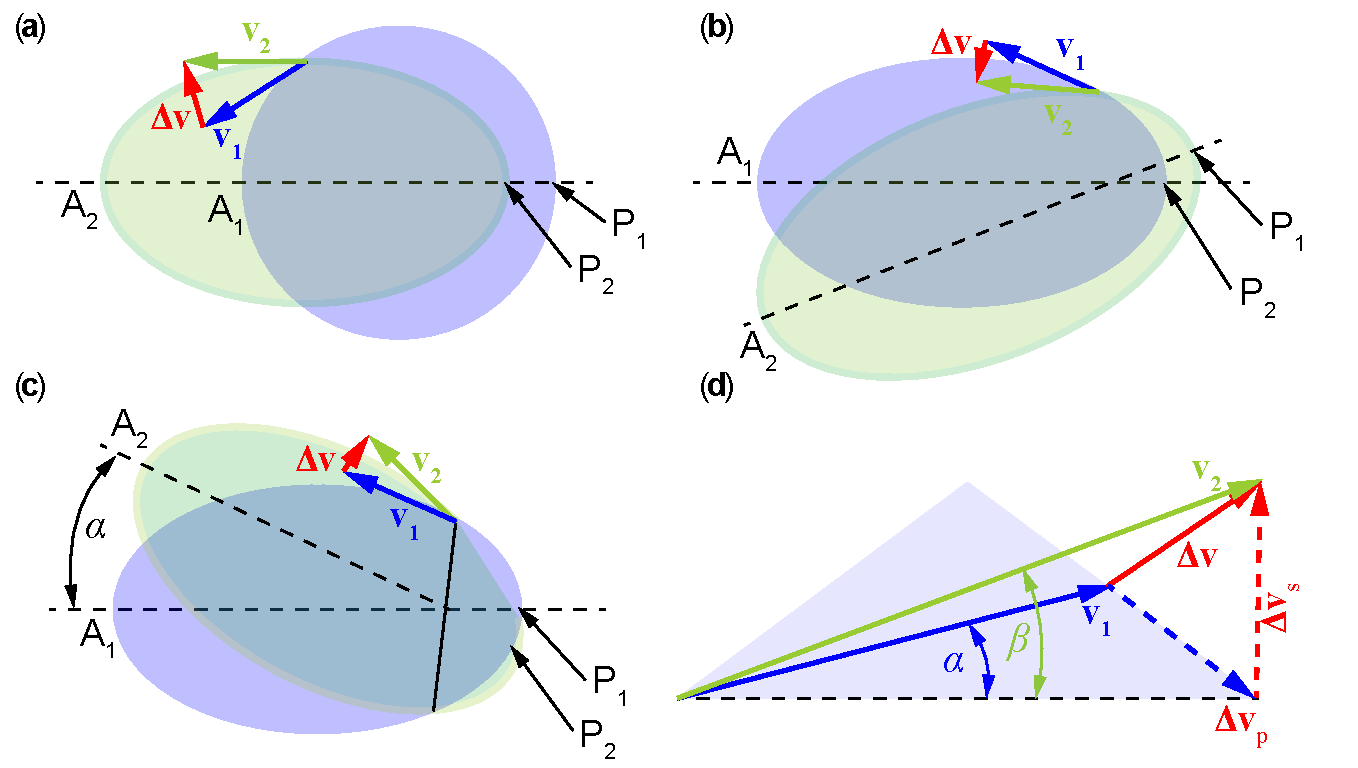
\includegraphics[width=\textwidth]{Bahnmanoever.pdf} 
	\caption[Wirkung der Geschwindigkeits�nderung auf Satellitenbahnen.]{Wirkung der Geschwindigkeits�nderung auf Satellitenbahnen. \fa �nderung der Exzentrizit�t. \fb �nderung der (Richtung) der Apsidenlinie. \fc �nderung der Inklination. \fd Vektorielle Addition der Geschwindigkeiten beim impulsiven Man�ver. Der Winkel $\alpha$ liegt wie $\Delta \vec{v}_\text{p}$ in der urspr�nglichen Bahnebene, der Winkel $\beta$ ebenso wie $\Delta \vec{v}_\text{s}$ senkrecht zur urspr�nglichen Bahnebene.}
	\label{abb:adyn_manenvers_overview}
\end{figure}

F�r impulsive Schubphasen kann die Wirkung der Geschwindigkeits�nderung je nach vektorieller Addition nach folgenden Gesichtspunkten unterteilt werden (\figref{adyn_manenvers_overview}).
\begin{enumerate}
    \item [1)] Koplanare Transfers, \dh die Bahnebene bleibt erhalten, wobei es entweder zu einer 
\begin{itemize}
        \item  �nderung der Exzentrizit�t bis hin zum �bergang in eine andere Bahnform oder
        \item  einer �nderung der Apsidenlinie kommt, oder alternativ zu einer
\end{itemize}
    \item [2)] �nderung der Inklination der Bahn f�hrt.
\end{enumerate}
Wir wollen uns zun�chst koplanare Transfers/Man�ver anschauen.

\subsubsection{Hohmann-Transfer}\label{kap:adyn_hohmann_transfer}

Als erstes Beispiel f�r ein impulsives koplanares Man�ver betrachten wir den Hohmann\indexp{Hohmann, Walter}\footnote{Walter Hohmann (1880--1945) war ein st�dtischer Baurat in Essen und besch�ftigte sich nebenberuflich mit Himmelsmechanik und Raumfahrt. Den nach ihm benannten Transfer zwischen zwei Satellitenbahnen beschrieb er bereits 1925 in seinem Buch "`Die Erreichbarkeit der Himmelsk�rper"'.}-Transfer. Der Hohmann-Transfers besteht darin, einen Satelliten aus einer niedrigeren (kreisf�rmigen) Umlaufbahn durch zwei Schubman�ver mit $\Delta v_1$  und $\Delta v_2$ auf eine Kreisbahn mit gr��erem Radius zu "`heben"' (\figref{adyn_hohmann_transfer}a).
Wir wollen als Beispiel berechnen, wie man einen Satelliten von einer Kreisbahn mit $h_1$ auf eine Kreisbahn der H�he $h_2$ bringen kann. \\
Dann muss der Satellit vor \bzw nach den Man�vern die Geschwindigkeiten 
\begin{align}
    v_1 = \sqrt{\frac{G\,m_\text{E}}{r_1}}= \sqrt{\frac{G\,m_\text{E}}{R_\text{E}+h_1}} ~~\text{\bzw}~~ 
		v_2 = \sqrt{\frac{G\,m_\text{E}}{r_2}}= \sqrt{\frac{G\,m_\text{E}}{R_\text{E}+h_2}} \label{eq:adyn_hohmann01}
\end{align}
haben.
\begin{figure}[H]
	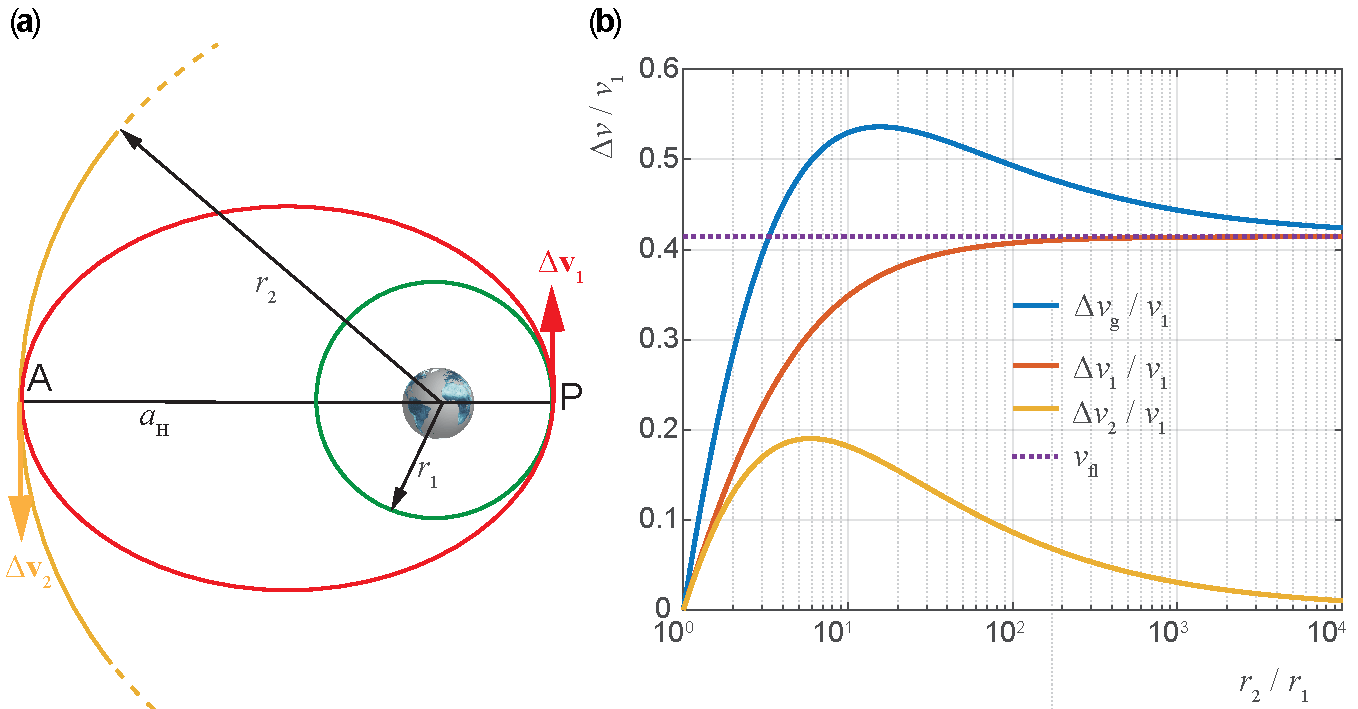
\includegraphics[width=\textwidth]{HohmannTransfer.pdf} 
	\caption[Hohmann-Transfer Prinzip und Geschwindigkeits�nderung.]{\fa Hohmann-Transfer Prinzip und \fb Geschwindigkeits�nderung bei Hohmann-Transfer als Funktion der Radius�nderung.}
	\label{abb:adyn_hohmann_transfer}
\end{figure}
Durch das erste Bahnman�ver mit $\Delta v_1$ kommt der Satellit aus einer Kreisbahn auf eine Transferellipse (Hohmann-Ellipse, \figref{adyn_hohmann_transfer}a), deren gro�e Halbachse durch 
\begin{align}
    a_\text{H} = \frac{1}{2}\,\lk r_1+r_2 \rk \label{eq:adyn_hohmann02}
\end{align}
gegeben ist. Nach der \gls{visvivaadyn} \eqref{eq:hm_vis-viva} \bzw \eqref{eq:adyn_orbit03} ergeben sich dann f�r diese Ellipse folgende Perig�ums- und Apog�umsgeschwindigkeiten:
\begin{subequations}
\begin{align}
    v_\text{P} &= \sqrt{G\,m_\text{E}}\,\sqrt{\frac{2}{r_1}-\frac{1}{\frac{1}{2}\,\lk r_1+r_2\rk}} = \sqrt{\frac{G\,m_\text{E}}{a_\text{H}}\,\frac{r_2}{r_1}} \,,\label{eq:adyn_hohmann03a}\\
    v_\text{A} &= \sqrt{G\,m_\text{E}}\,\sqrt{\frac{2}{r_2}-\frac{1}{\frac{1}{2}\,\lk r_1+r_2\rk}} = \sqrt{\frac{G\,m_\text{E}}{a_\text{H}}\,\frac{r_1}{r_2}}\,.\label{eq:adyn_hohmann03b}
\end{align}
\end{subequations}
Im Apog�um\index{Apog�um} der Transferellipse muss eine zweite Schubphase mit $\Delta v_2$ erfolgen, die aus der Ellipsenbahn wieder eine Kreisbahn mit der Geschwindigkeit $v_2$ nach \eqref{eq:adyn_hohmann01} macht, \dh wir haben insgesamt eine Geschwindigkeits�nderung von 
\begin{align}
    \Delta v = \Delta v_1+ \Delta v_2 = \lk v_\text{P}-v_1\rk +\lk v_2-v_\text{A}\rk\,.\label{eq:adyn_hohmann04}
\end{align}
In \figref{adyn_hohmann_transfer}b ist der Antriebsbedarf $\Delta v$ als Funktion des Radienverh�ltnisses $r_2/r_1$ dargestellt. Man erkennt, dass f�r bestimmte Radienverh�ltnisse der gesamte Geschwindigkeitsbedarf $\Delta v$ gr��er als die \gls{vescape} werden kann (\probref{adyn_manoevers1}).
%BEISPIEL 1 %%%%%%%%%%%%%%%%%%%%%%%%%%%%%%%%%%%%%%%%%%%%%%%%%%%%%%%%%%%%%%%%%%%%%%%%%%%%%%%%%
\begin{example}{Hohmann-Transfer f�r kleine Bahn�nderungen}  
Wir wollen jetzt noch eine N�herung f�r den Geschwindigkeitsbedarf beim Hohmann-Transfer f�r kleine Bahn�nderungen $\Delta r$ herleiten.
Wir erhalten f�r kleine Bahn�nderungen
	\[\frac{\Delta r}{r_1} = \frac{r_2-r_1}{r_1} \approx \frac{\Delta r}{r}~~\rightarrow~~r_2 \approx \Delta r+ r_1\,.
\]
Unter Verwendung von $a_\text{H} = r_1 +\Delta r / 2$ folgt damit:
\begin{align}
\begin{split}
    v_2 &= \sqrt{\frac{G\,m_\text{E}\,r_1}{r_2\,r_1}} = v_1\,\sqrt{\frac{r_1}{r_2}} \approx v_1 \,\sqrt{\frac{r_1}{r_1+\Delta r}} \approx v_1\,\lk 1-\frac{1}{2}\,\frac{\Delta r}{r}\rk\,,\\ 
    v_\text{P}&= v_1\,\lk 1+\frac{1}{4}\,\frac{\Delta r}{r}\rk\;, ~~~v_\text{A} = v_1\,\lk 1-\frac{3}{4}\,\frac{\Delta r}{r}\rk\,, 
\end{split} \label{eq:adyn_hohmann05}
\end{align}
woraus folgt:
\begin{align}
    \Delta v &= \killA{v_1} + \frac{v_1}{4}\,\frac{\Delta r}{r}-\killA{v_1} + \killA{v_1} - \frac{v_1}{2}\,\frac{\Delta r}{r}-\killA{v_1} + \frac{3}{4}\,v_1\,\frac{\Delta r}{r} \ = \frac{1}{2}\,v_1\,\frac{\Delta r}{r} \,. \label{eq:adyn_hohmann06}
\end{align} 
\end{example} \label{bsp:adyn_hohmann_klein}
%BEISPIEL %%%%%%%%%%%%%%%%%%%%%%%%%%%%%%%%%%%%%%%%%%%%%%%%%%%%%%%%%%%%%%%%%%%%%%%%%%%%%%%%%%

\subsubsection{Hohmann-, Oberth- und Edelbaum-Transfers nach Unendlich}\label{kap:adyn_oberth_edelbaum}

\begin{figure}[H]
	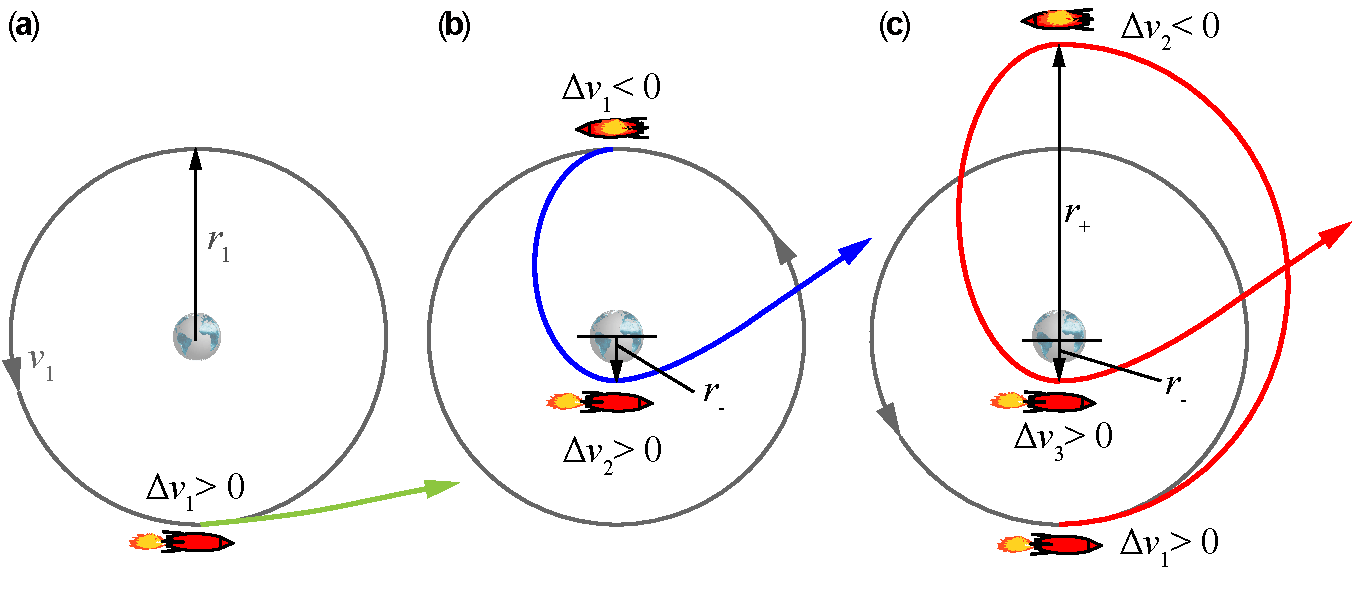
\includegraphics[width=\textwidth]{TransfersInfin01.pdf} 
	\caption[Hohmann-, Oberth- und Edelbaum-Transfers nach Unendlich.]{\fa Hohmann-, \fb Oberth- und \fc Edelbaum-Transfers nach Unendlich ($\infty$).}
	\label{abb:adyn_Oberth_transfer1}
\end{figure}

In vorherigen \kap{adyn_hohmann_transfer} hatten wir den Hohmann-Transfer von Satelliten von einer kreisf�rmigen Ausgangsbahn mit Radius $r_1$ auf eine elliptische Bahn mit der gro�en Halbachse $a_\text{H}$ und anschlie�end auf eine Kreisbahn mit $r_2$ untersucht, wobei $a_\text{H} = \frac{1}{2}\,\lk r_1+r_2\rk$ war. \\
Man kann sich jetzt die Frage stellen, wie gro� die notwendige Geschwindigkeits�nderung sein muss, damit der Satellit aus der Umlaufbahn $r_1$ nach $r_2=\infty$ kommt, also den Gravitationsbereich der Erde (\bzw des jeweiligen Zentralk�rpers) verl�sst. Wie gro� ist seine Flugzeit in einem solchen Fall, bis der Satellit \zb einen Abstand $200\,r_1,\,500\,r_1,\,1000\,r_1$ von der Erde erreicht (siehe auch \probref{adyn_manoevers2})?\\
Man kann sich auch �berlegen, dass es neben diesem sogenannten direkten Transfer auf die Endgeschwindigkeit $v_\infty$ (im Prinzip ein entarteter Hohmann-Transfer auf eine Hyperbel) zwei m�gliche weitere Transfers mit insgesamt zwei \bzw drei impulsiven Schubman�vern geben kann. Diese werden als Oberth-\indexp{Oberth, Hermann Julius} \bzw Edelbaum\indexp{Edelbaum, Theodore}\footnote{Theodore N. Edelbaum war ein US-amerikanischer Astrodynamiker und Raumfahrtspezialist.}-Transfers oder auch Zwei- \bzw Drei-Impuls-Transfers bezeichnet (\figref{adyn_Oberth_transfer1}).\\
Wir berechnen die notwendigen $\Delta v$ f�r die 3 F�lle, die entsprechende Flugzeit und den Treibstoffverbrauch und folgen dabei der Darstellung in \cite{Blanco2021}. Bei der L�sung benutzen wir:
\begin{enumerate}
    \item Die Energiegleichung (Notation entsprechend \kap{hm_bewegungsgl}):
    \begin{align}
        H = \frac{1}{2}\,v^2 -\frac{G\,m_\text{E}}{r}\,. \label{eq:adyn_escape01}
    \end{align}
		\item Die asymptotische Geschwindigkeit $v_\infty$ im Unendlichen ergibt sich dann:
    \begin{align}
        \frac{1}{2}\,v_\infty{}^2 &= \frac{1}{2}\,v_\text{Start} - \frac{G\,m_\text{E}}{r_\text{Start}}~~~\rightarrow ~~~ v_\text{Start} = \sqrt{\frac{2\,G\,m_\text{E}}{r_\text{Start}} + v_\infty{}^2} \,. \label{eq:adyn_escape02} 
    \end{align}
    Hierin sind $v_\text{Start},\,r_\text{Start}$ die Geschwindigkeit \bzw der Radius nach dem Starten des Man�vers. Man beachte, dass $v_\text{Start}$ f�r $v_\infty > 0$ verschieden von der f�r die Erde definierten Fluchtgeschwindigkeit $v_\text{F} = \sqrt{2\,G\,m_\text{E} / R_\text{E}}$ ist.
		\item Die Definition des Drehimpulses f�r eine Kreisbahn \bzw Ellipsenbahn (A\,Apog�um\,,\,P Perig�um)\index{Apog�um}\index{Perig�um} lautet:
    \begin{align}
    \begin{split}
        L &= r_1\,v_1~~~~ \text{Kreisbahn}\,,~~~\text{\bzw}~~~ L = r_\text{A}\,v_\text{A} = r_\text{P}\,v_\text{P}~~~~ \text{Ellipse} \,,\\
				&\text{mit} ~~ r_\text{P},\,r_\text{A} ~~~\text{Abstand zum Perig�um \bzw Apog�um}\,.
    \end{split}\label{eq:adyn_escape03} 
    \end{align}
    \item F�r die Geschwindigkeit beim Apo- \bzw Perig�um kann man aus der Drehimpulserhaltung leicht ableiten:
    \begin{align}
        v_\text{A} &= \sqrt{\frac{G\,m_\text{E}}{r_\text{A}}} \,\sqrt{\frac{2}{1+r_\text{A}/r_\text{P}} }\, ~~~ \text{\bzw}~~~
        v_\text{P} = \sqrt{\frac{G\,m_\text{E}}{r_\text{P}}} \,\sqrt{\frac{2}{1+r_\text{P}/r_\text{A}} }\,. \label{eq:adyn_escape04}
    \end{align}
\end{enumerate}		
		Wir schauen uns nun die einzelnen Transfers an, wobei wir den Radius der Ausgangsbahn jetzt mit $r_0$ bezeichnen wollen.
\begin{itemize} 
		\item \underline{Fall A:} Direkter Transfer aus einer Kreisbahn mit Radius $r_1$ (Hohmann-Transfer nach $\infty$) \\
    Aus \eqref{eq:adyn_escape02} erhalten wir
    \begin{align}
		\begin{split}
        v_\text{Start} &= v_1 +\Delta v_\text{A} = \sqrt{\frac{2\,G\,m_\text{E}}{r_1} + v_\infty{}^2}\qquad\text{und mit} \qquad v_1 = \sqrt{\frac{G\,m_\text{E}}{r_1}}   \,,\\
         \rightarrow ~~~~ \Delta v_\text{A} &= v_1\,\lk \sqrt{2+\frac{v_\infty{}^2}{v_1{}^2}}-1\rk = v_1\,\lk \sqrt{2+\frac{v_\infty{}^2\,r_1}{G\,m_\text{E}}}-1\rk \,.
		\end{split} \label{eq:adyn_escape06}
    \end{align}
    \item \underline{Fall B:} Zwei-Impuls-Transfer (Oberth-Transfer)\\
		Die physikalischen Grundlagen des Oberth-Effektes\index{Oberth-Effekt} und damit des Oberth-Transfers sind ausf�hrlich in \probref{adyn_rocket_analogy} behandelt und sollen hier als bekannt voraus gesetzt werden.
    \begin{itemize}
        \item F�r den ersten Impuls, bei dem es zu einer Abbremsung aus der initialen Kreisbahn mit $r_1$ auf eine kleinere Ellipsenbahn mit Perig�umsabstand $r_\text{-}$ kommt, finden wir am Punkt $A$ (Apog�um)
        \begin{align}
            \Delta v_{\text{B},1} &= v_\text{A} -v_1 = \sqrt{\frac{G\,M}{r_1}}\,\lk \sqrt{\frac{2}{1+\frac{r_1}{r_\text{-}}}}\rk-v_1 = -v_1\,\lk 1-\sqrt{\frac{2}{1+\frac{r_1}{r_\text{-}}}}\rk \label{eq:adyn_escape07}\,.
        \end{align}
        \item Beim Perig�um $P$, wo $r=r_\text{-}$ ist und der zweite Impuls erfolgt, finden wir
        \begin{align}
            \Delta v_{\text{B},2} &= v_\text{Start} - v_\text{P} = \sqrt{\frac{2\,G\,m_\text{E}}{r_\text{-}} + v_\infty{}^2} - \sqrt{\frac{G\,m_\text{E}}{r_\text{-}}}\,\sqrt{\frac{2}{1+r_\text{-} / r_1}}\nonumber \\
            &= \sqrt{\frac{G\,m_\text{E}}{r_1}}\,\lk \sqrt{2+\frac{v_\infty{}^2\,r_\text{-}}{G\,m_\text{E}}} - \sqrt{\frac{2}{1+r_\text{-} / r_1}}\rk \,. \label{eq:adyn_escape08}
        \end{align}
        \item Der gesamte notwendige Antriebsbedarf ist dann
        \begin{align}
            \Delta v_\text{B} = |\Delta v_\text{B,1}| + \Delta v_\text{B,2} = v_1\,\lk 1+\sqrt{\frac{v_\infty{}^2}{v_1{}^2} + \frac{2r_1}{r_\text{-}}} - \sqrt{2+\frac{2r_1}{r_\text{-}}}\rk \label{eq:adyn_escape09}\,.
        \end{align}
    \end{itemize}
    \item \underline{Fall C:} Drei-Impuls-Transfer (Edelbaum-Transfer)
    \begin{itemize}
        \item Im ersten Schritt geht das Raumschiff auf eine gr��ere elliptische Bahn mit einer gro�en Halbachse $r_\text{+}$:
        \begin{align}
            \Delta v_\text{C,1} = v_1\,\lk \sqrt{\frac{2}{1+\frac{r_1}{r_\text{+}}}} -1\rk\,. \label{eq:adyn_escape10} 
        \end{align}
        \item Im zweiten Schritt wird es wieder auf eine deutlich kleinere Bahn mit Radius $r_\text{Ed2}$ gebracht (durch Abbremsen):
        \begin{align}
            \Delta v_\text{C,2} = -\sqrt{\frac{G\,m_\text{E}}{r_\text{+}}}\,\lk \sqrt{\frac{2}{1+r_\text{+} / r_1}} - \sqrt{\frac{2}{1+r_\text{+} / r_\text{-}}}\rk \,. \label{eq:adyn_escape11} 
        \end{align}
        \item Im dritten Schritt wird das Raumschiff wieder beschleunigt:
        \begin{align}
            \Delta v_\text{C,3} = \sqrt{\frac{G\,m_\text{E}}{r_\text{-}}}\,\lk \sqrt{2+\frac{v_\infty{}^2\,r_\text{-}}{G\,m_\text{E}}} - \sqrt{\frac{2}{1+r_\text{-}/ r_\text{+}}}\rk\,.\label{eq:adyn_escape12} 
        \end{align}
        \item Die gesamte Geschwindigkeits�nderung ist:
        \begin{align}
            \Delta v_\text{C} &= \Delta v_\text{C,1} + |\Delta v_\text{C,2}| + \Delta v_\text{C,3} \nonumber \\
            &= v_1\,\lk \sqrt{\frac{v_\infty{}^2}{v_1{}^2} + \frac{2r_1}{r_\text{-}}} + \sqrt{2 + \frac{2r_1}{r_\text{+}}} - \sqrt{\frac{2r_1}{r_\text{-}}+\frac{2r_1}{r_\text{+}}}- 1\rk\,.\label{eq:adyn_escape13} 
        \end{align}
    \end{itemize}
\end{itemize}
Man kann nun vergleichen, wie sich die $\Delta v$ f�r die verschiedenen F�lle verhalten  (\figref{adyn_Oberth_transfer2}) und erkennt, dass f�r gr��ere $v_\infty$ das Edelbaum-Man�ver einen geringeren Antriebsbedarf (und damit geringeren Treibstoffbedarf) hat als der Oberth- und auch der direkte Transfer. 
Aus \eqref{eq:adyn_escape13} erh�lt man durch Invertierung auch eine Beziehung f�r $v_\infty\,\lk v_1,r_1,r_\text{-},r_\text{+}\rk$ bei gegebenen Treibstoffvorrat $\Delta v$:
\begin{align}
    v_\infty = v_1\,\sqrt{ \lek 1+\frac{\Delta v}{v_1} + \sqrt{\frac{2r_1}{r_\text{-}} + \frac{2r_1}{r_\text{+}}} - \sqrt{2+\frac{2r_1}{r_\text{+}}} \rek^2 - \frac{2\,r_1}{r_\text{-}} }\,.\label{eq:adyn_escape14} 
\end{align}
F�r $r_\text{+} = r_1$ ergibt sich die Beziehung f�r den Oberth-Transfer, f�r $r_\text{-} = r_\text{+} = r_1$ die f�r den direkten Transfer.
%BEISPIEL 2 %%%%%%%%%%%%%%%%%%%%%%%%%%%%%%%%%%%%%%%%%%%%%%%%%%%%%%%%%%%%%%%%%%%%%%%%%%%%%%%%%
\begin{example}{Flugbahnen und Flugzeiten f�r die Hohmann-Oberth-Edelbaum-Transfers}  
Zum Schluss adressieren wir die Frage, welches das Flugman�ver (Hohmann-, Oberth- oder Edelbaum-Transfer) mit dem geringsten Treibstoffverbrauch \bzw mit der k�rzesten Flugzeit ist.
Die Energie des Systems Raumschiff und ausgestr�mtes Gas nach dem jeweiligen i-ten Schubimpuls ist:
\begin{align}
	E_\text{g} &= T_\text{g, i} + \Delta E_\text{chem} = -\frac{1}{2}\, m_\text{i} v_1{}^2 + \frac{1}{2}\, \lk m_\text{i} - m_\text{f} \rk v_\text{G}{}^2 \nonumber \\
	           &= -\frac{1}{2}\, m_\text{i} v_1{}^2 + \frac{1}{2}\,  m_\text{i}\,v_\text{G}{}^2 \lk 1 - \e^{\lk - \Delta v / v_\text{G} \rk} \rk \,. \label{eq:adyn_oberth31}
\end{align}
Hierin ist wie bisher $m_\text{i}$ die Gesamtmasse des Raumschiffs inklusive Treibstoff vor dem Schubman�ver, $m_\text{f}$ die Masse danach, $v_\text{G}$ die Ausstr�mgeschwindigkeit des Treibstoffgases und $\Delta E_\text{chem} $ die w�hrend des Schubs umgesetzte chemische Energie des Treibstoffs. Wenn man $v_\text{G} = \kappa\,v_1$ setzt, dann kann man die �nderung der kinetischen Energie des Raumschiffs pro impulsivem Schubman�ver relativ einfach berechnen.\\ %Dies werden wir in \probref{adyn_manoevers1} tun. \\
F�r die Berechnung der Flugzeiten muss man beachten, dass sich die Gesamtzeit aus Segmenten einer hyperbolischen Bahn und Segmenten von elliptischen Bahnen (genauer halben Ellipsen) zusammensetzt. Die Berechnung der Halbellipsen-Zeiten (\zb von $r_\text{out}$ bis $r_\text{in}$) ist nach dem 3. Keplerschen Gesetz:
\begin{align}
	t_\text{ell} = \frac{1}{2}\,2\pi \sqrt{\frac{a^3}{G\,m_\text{E}}} = \frac{\pi}{2} \sqrt{\frac{\lk r_\text{A} + r_\text{P} \rk^3}{2\,G\,m_\text{E}}} \,. \label{eq:adyn_oberth32}
\end{align}
Die Berechnung des hyperbolischen Abschnitts ist etwas komplexer. Wir starten dazu von der Gleichung f�r den Radialanteil der Geschwindigkeit (vgl. \eqref{eq:hm_allg_ZK_2}):
\begin{align}
	v_r{}^2 = \lk \frac{\D r}{\D t}\rk^2 = v_\infty{}^2 + 2 \,\frac{G\,m_\text{E}}{r} - \frac{L^2}{r^2}  \,. \label{eq:adyn_oberth33}
\end{align}
Wir wissen, dass am Perig�um gilt:
\begin{align}
   \frac{\D r}{\D t} &= 0 ~~~\rightarrow~~~ L^2 = v_\infty{}^2\,r_\text{P}{}^2 + 2 \,G\,m_\text{E}\,r_\text{P} ~~~\text{und erhalten somit} \nonumber \\
	 \frac{\D r}{\D t} &= \sqrt{ v_\infty{}^2 + 2 \,\frac{G\,m_\text{E}}{r} - \frac{v_\infty{}^2\,r_\text{P}{}^2 + 2 \,G\,m_\text{E}\,r_\text{P}}{r^2}} \,.  \label{eq:adyn_oberth34}
\end{align}
Diese DGL 1. Ordnung kann man numerisch mit den �blichen Verfahren in \matlab{}\, integrieren, alternativ kann man die inverse Funktion $t(r)$ durch Integration von
\begin{align}
	 \frac{\D t}{\D r} = \frac{r}{\sqrt{ v_\infty{}^2 \lk {r^2 -r_\text{P}{}^2}\rk + 2 \,G\,m_\text{E} \lk {r -r_\text{P}}\rk }} \label{eq:adyn_oberth35}
\end{align}
berechnen. Mit Hilfe einer Integraltafel \cite{Gradshteyn1980} findet man:
\begin{align}
\begin{split}
	 t_\text{hyp}(r, r_\text{P}) &= \frac{G\,m_\text{E}}{v_\infty{}^3} \lek \sqrt{\lk 1+ \frac{r\,v_\infty{}^2}{G\,m_\text{E}}\rk^2 - \lk 1 + \frac{r_\text{P}\,v_\infty{}^2}{G\,m_\text{E}}\rk^2 }\rek + \ldots \\
	      &~~~ + \frac{G\,m_\text{E}}{v_\infty{}^3} \ln{\lek \frac{G\,m_\text{E} + v_\infty{}^2\,r}{v_\infty\, \sqrt{ v_\infty{}^2 \lk {r^2 -r_\text{P}{}^2}\rk + 2 \,G\,m_\text{E} \lk {r -r_\text{P}}\rk }}\rek}\\
				&= \frac{T_0}{2\pi} \frac{v_1{}^3}{v_\infty{}^3} \lek \sqrt{\lk 1 + \frac{r\,v_\infty{}^2}{r_1\,v_1{}^2} \rk^2 - \lk 1 + \frac{r_\text{P}\,v_\infty{}^2}{r_1\,v_1{}^2} \rk^2 } -
				    \cosh^{-1} {\lk \frac{1 + \frac{r\,v_\infty{}^2}{r_1\,v_1{}^2}}{1 + \frac{r_\text{P}\,v_\infty{}^2}{r_1\,v_1{}^2} } \rk} \rek \,.
\end{split} \label{eq:adyn_oberth36}
\end{align}
\label{bsp:adyn_transfers_times}
F�r die weitere Diskussion verweisen wir auf \probref{adyn_manoevers3}.\\

\end{example}
%BEISPIEL %%%%%%%%%%%%%%%%%%%%%%%%%%%%%%%%%%%%%%%%%%%%%%%%%%%%%%%%%%%%%%%%%%%%%%%%%%%%%%%%%%

\begin{figure}[H]
	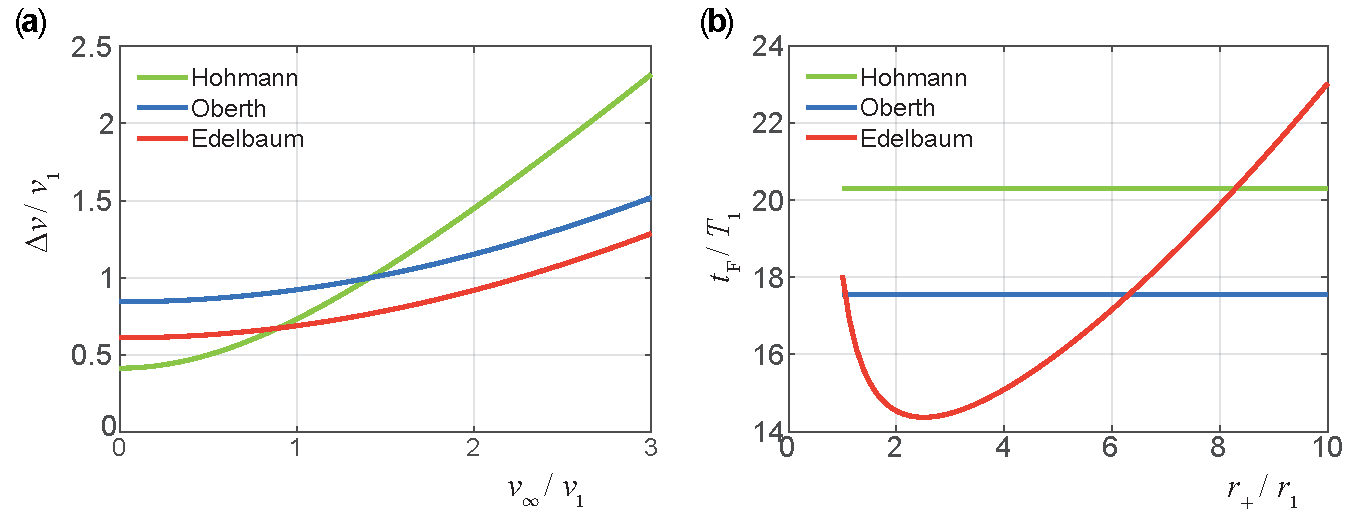
\includegraphics[width=\textwidth]{TransfersInfin02.pdf} 
	\caption[Geschwindigkeitsbedarf und Flugzeiten beim Transfer nach $\infty$.]{\fa Geschwindigkeitsbedarf f�r verschiedene zu erzielende Endgeschwindigkeiten beim Hohmann-, Oberth- \bzw Edelbaum-Transfer nach $\infty$. Man sieht, dass ab einer bestimmten zu erreichenden Endgeschwindigkeit das Geschwindigkeitsbudget f�r den Oberth- und Edelbaum-Transfer kleiner ist als das f�r den direkten Hohmann-Transfer. \fb Flugzeiten bis zu $r=200\,r_1$ beim Hohmann-, Oberth- \bzw Edelbaum-Transfer. Als variabler Parameter wurde der �u�ere Radius $r_{+}$ genommen, der innere Radius wurde als fix mit $r_{-}=0.05\,r_1$ gesetzt und der Schubparameter wurde mit $\Delta v/v1 = 1.1$ angenommen. Man erkennt, dass es f�r $r_{+}\approx 2.5\,r_1$ ein absolutes Minimum der Flugzeit f�r den Edelbaum-Transfer gibt. Danach f�hrt die l�ngere Flugzeit auf der Halbellipse von $r_{+}$ nach $r_{-}$ zu insgesamt l�ngeren Flugzeiten. (Nach \cite{Blanco2021}, siehe auch \probref{adyn_manoevers2}.)} \label{abb:adyn_Oberth_transfer2}
\end{figure}
Das Ergebnis der zeitlichen Entwicklung der verschiedenen Transfers ist in \probref{adyn_manoevers2} explizit durchgerechnet und das Ergebnis im Vergleich der verschiedenen Transfers in \figref{adyn_Oberth_transfer2} zu sehen. 

\subsection{Interplanetare Raumfl�ge zu den Nachbarplaneten der Erde}\label{kap:adyn_flight_venus_mars}

Wir wollen in diesem Kapitel Raumfl�ge zu Mars und Venus untersuchen und zun�chst stark vereinfachende Annahmen treffen, um Grundprinzipien bei der Planung einer solchen Mission zu verdeutlichen. Insbesondere sollen
\begin{enumerate}
    \item [1.] alle Bewegungen (Planeten, Raumsonde) koplanar in der Ekliptik stattfinden,
		\item [2.] die Planetenbahnen als kreisf�rmig angenommen werden und
		\item [3.] der Flug zum Nachbarplaneten �ber eine Hohmann-Ellipse erfolgen.
\end{enumerate}
Zun�chst betrachten wir den Flug zur Venus, f�r welchen gilt:
\begin{align}
\begin{split}
    \upsilon_\text{E}  &= \upsilon_\text{E}\lk t_0\rk + n_\text{E}\,\lk t-t_0\rk = \upsilon_\text{E,0} + n_\text{E}\,t\,,\\
    \upsilon_\text{V}  &= \upsilon_\text{V}\lk t_0\rk + n_\text{V}\,\lk t-t_0\rk = \upsilon_\text{V,0} + n_\text{V}\,t\,.
\end{split} \label{eq:adyn_PlFlights01}
\end{align} 
Hierin sind $n_\text{E},\,n_\text{V},\,n_\text{M}$ die mittleren Bewegungen\index{Bewegung!mittlere} der Planeten Erde, Venus \bzw f�r sp�ter auch Mars (siehe Tabelle \ref{tab:hm_bahnparameter}), die sich nach \eqref{eq:adyn_Bahnpara05} berechnet. Die Differenz der wahren Anomalien $\psi = \upsilon_\text{V} -\upsilon_\text{E}$ wird als Phasenwinkel zwischen Venus und Erde bezeichnet. Dessen zeitliche Entwicklung lautet:
\begin{align}
    \psi = \psi_0 + \lk n_\text{V} - n_\text{E}\rk\,t ~~~~ \text{mit} ~~~~ \psi_0 = \upsilon_\text{V,0} - \upsilon_\text{E,0}\,. \label{eq:adyn_PlFlights02}
\end{align}
Aus \eqref{eq:adyn_PlFlights02} folgt die bereits in der \probref{hm_sideric_period_mars} hergeleitete synodische Periode\index{Periode!Synodische} eines Planeten (hier der Venus). Diese synodische Periode ergibt sich als die Zeit, die verstreicht, bis der Phasenwinkel zwischen den beiden betrachteten Himmelsk�rpern wieder den gleichen Wert hat.
\begin{align}
    \psi_0 +2k\pi &= \psi_0 +\lk n_\text{V} - n_\text{E}\rk\,T_\text{syn}\nonumber\\
    \rightarrow ~~~~ T_\text{syn,V} &= \frac{2\pi}{n_\text{V}-n_\text{E}} = \frac{2\pi}{2\pi\,\lk \frac{1}{T_\text{P,V}} - \frac{1}{T_\text{P,E}}\rk} = \frac{T_\text{P,E} T_\text{P,V}}{T_\text{P,E} - T_\text{P,V}}\label{eq:adyn_PlFlights03}\,.
\end{align}
Analog gilt f�r den Mars:
\begin{align}
    T_\text{syn,M} = \frac{2\pi}{n_\text{E}-n_\text{M}} = \frac{T_\text{P,M} T_\text{P,E}}{T_\text{P,M} - T_\text{P,E}}\label{eq:adyn_PlFlights04}\,.
\end{align}
Da der Transfer �ber eine Hohmann-Ellipse mit der gro�en Halbachse $a_\text{H}$ erfolgen soll (vgl. auch \kap{adyn_hohmann_transfer}), findet man mit \figref{adyn_flight_venus_mars}b,c und dem sog. \gls{gravparadyn}\index{Gravitationsparameter}~$\mu_\text{S}=G\,m_\text{S}$ leicht den finalen Phasenwinkel $\psi_\text{f}$:
\begin{align}
\begin{split}
  a_\text{H} &= \frac{1}{2}\,\lk r_\text{E} + r_\text{M}\rk\,,\,~~t_\text{H} = \frac{1}{2} \frac{2\pi}{n_\text{H}} = \pi\,\sqrt{\frac{a_\text{H}{}^3}{\mu_\text{S}}}\,~~\text{und}~~ \pi = \psi_0 + n_\text{M}\,t_\text{H}\;, ~~~\\
 \psi_\text{f} &= \psi_0 + t_\text{H}\,\lk n_\text{M}-n_\text{E}\rk = \pi -n_\text{E}\,t_\text{H}\;.
\end{split}\label{eq:adyn_PlFlights05}
\end{align}
Damit liegen die Phasenwinkel zwischen Erde und Mars bei Start und Ankunft fest. Als Werte ergeben sich $t_\text{H} \approx 259\,\text{d}$, $\psi_0 \approx 44.3\degree$ und $\psi_\text{f} \approx -75.1\degree$. \\
Ein negativer Phasenwinkel $\psi_\text{f}$ bedeutet, dass der Mars \anf{hinter} der Erde liegt (\figref{adyn_flight_venus_mars}c), also $\upsilon_\text{f, M} < \upsilon_\text{f, E}$.

\begin{figure}[H]
	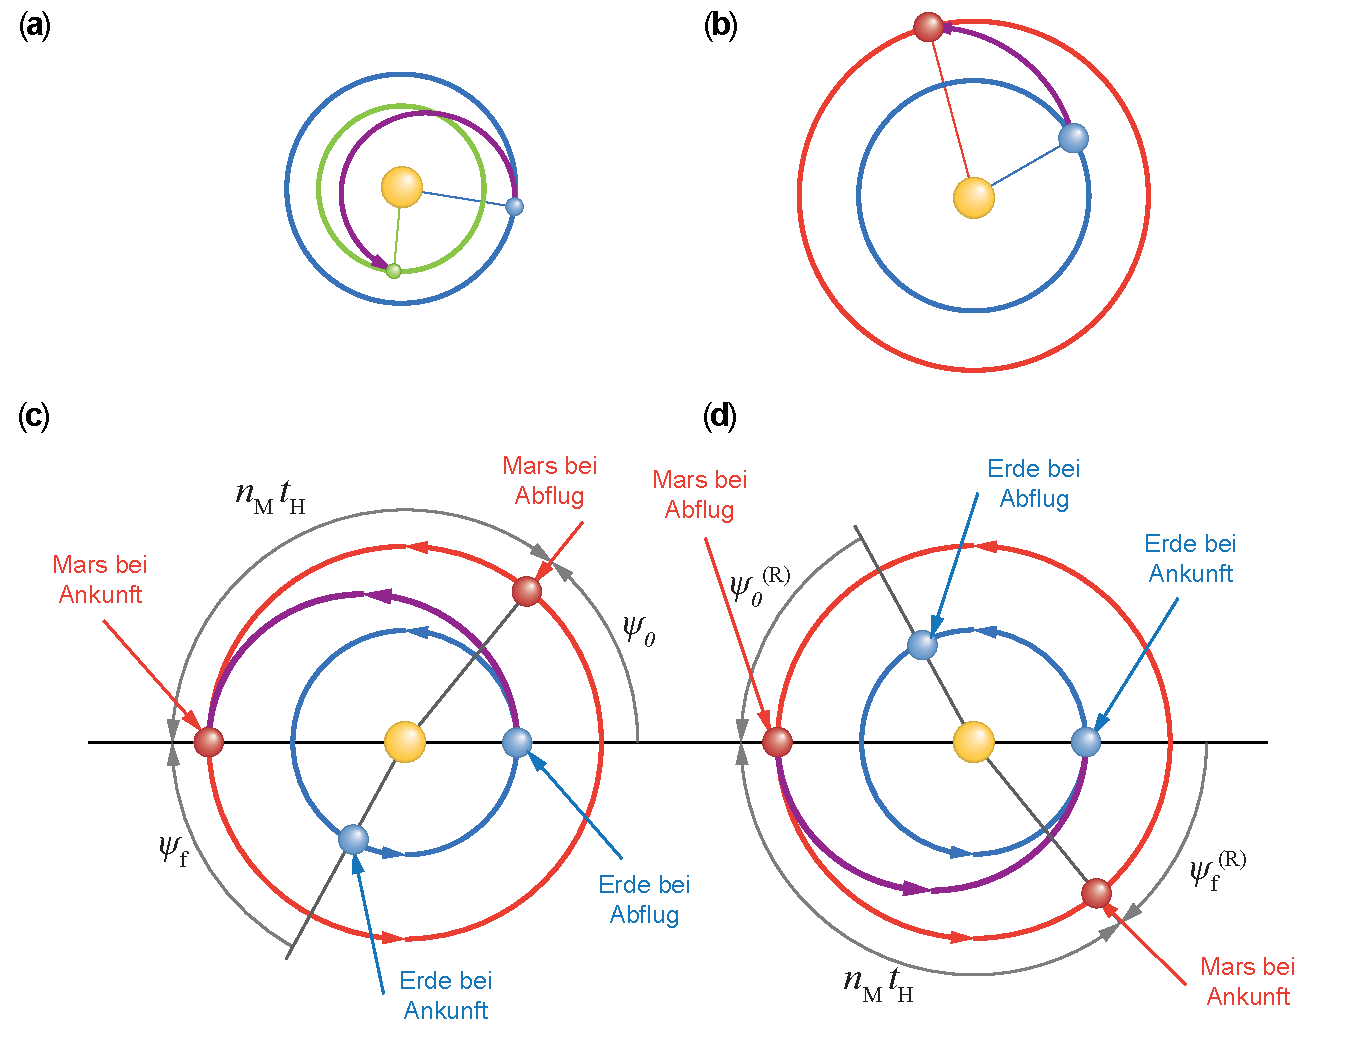
\includegraphics[width=\textwidth]{InterplanetarerTransfer.pdf} 
	\caption[Raumfl�ge zu Venus und Mars.]{Raumfl�ge zu Venus und Mars. \fa Raumflug zur Venus (ma�st�blich, Reisezeit 158 Tage). \fb Raumflug zum Mars (ma�st�blich, Reisezeit 115 Tage).  \fc Raumflug von der Erde zum Mars (nicht ma�st�blich). Beziehung der Phasenwinkel $\psi_0, \psi_\text{f}$ beim Hinflug von der Erde zum Mars. \fd Raumflug vom Mars zur Erde (nicht ma�st�blich). Beziehung der Phasenwinkel $\psi_0{}^\text{(R)}, \psi_0, \psi_\text{f}$ beim R�ckflug vom Mars zur Erde.}
	\label{abb:adyn_flight_venus_mars}
\end{figure}

F�r die R�ckkehr zur Erde geht man eine \anf{umgekehrte} Hohmann-Ellipse aus, was nichts anderes bedeutet als:
\begin{align}
    \psi_0{}^\text{(R)} = -\psi_\text{f}\,.\label{eq:adyn_PlFlights06R}
\end{align}
Die Raumsonde muss aber eine gewisse Zeit $t_\text{W}$ auf dem Mars warten, bis die Konstellation nach \eqref{eq:adyn_PlFlights06R} eintritt (\figref{adyn_flight_venus_mars}b). Wegen
\begin{align}
    0 = 2\psi_\text{f} + \lk n_\text{M} - n_\text{E} \rk \,t_\text{W} \label{eq:adyn_PlFlights06R1}
\end{align}
und der Forderung, dass $t_\text{W}>0$ ist, muss man gegebenenfalls einen Betrag von $2k\pi$ mit $k=0, \pm 1, \pm 2\ldots $ zu \eqref{eq:adyn_PlFlights06R1} addieren, woraus folgt:
\begin{align}
    t_\text{M, W} = \frac{2\psi_\text{f} + 2\,\pi\,N}{n_\text{E}-n_\text{M}} \,.\label{eq:adyn_PlFlights06M}
\end{align}
Wir erhalten $t_\text{W} \approx 454\,\text{d}$, was bedeutet, dass eine Reise zum Mars �ber Hohmann-Bahnen im Minimum:\
$t_\text{M, ges} = t_\text{H} + t_\text{W} +  t_\text{H} \approx 259\,\text{d} + 454\,\text{d} + 259\,\text{d} = 972\,\text{d}$\
dauern wird. Entsprechend erh�lt man f�r die Venus:
\begin{align}
    t_\text{V, W} = \frac{2\psi_\text{f} - 2\,\pi\,N}{n_\text{V}-n_\text{E}} \,,\label{eq:adyn_PlFlights06V}
\end{align}
mit $N=0$ die Werte $t_\text{V, ges} = t_\text{H} + t_\text{V, W} +  t_\text{H} \approx 146\,\text{d} + 117\,\text{d} + 146\,\text{d} = 409\,\text{d}$\,.\\

Wir wollen nun auch Fl�ge untersuchen und berechnen, die nicht �ber Hohmann-Ellipsen ablaufen und bei denen die Positionsvektoren der Zielplaneten auch nicht mehr in der Ekliptikebene liegen m�ssen. Ferner soll eine bestimmte Flugzeit vorgegeben sein. Es sind dann der vom Hohmann-Transfer verschiedene Antriebsbedarf $\Delta \vec{v}$ und die Parameter der Transferbahn zu bestimmen. Dies f�hrt auf das im n�chsten Kapitel behandelte Lambert-Problem.

\subsection{Lambert-Problem (Lambert-Transfer)}\label{kap:adyn_lambert_transfer}\index{Lambert-Transfer}\index{Lambert-Problem|textbf}

Das Lambert\indexp{Lambert, Johann Heinrich}\footnote{Johann Heinrich Lambert (1728 -- 1777) war ein hugenottischer Schweizer Mathematiker und Physiker, der sich auch mit Kartographie und Astronomie besch�ftigte. Neben dem Lambert-Problem der Himmelsmechanik ist auch das Lambert-Beersche Gesetz der Lichtabsorption nach ihm benannt.}\index{Lambert-Problem}-Problem lautet wie folgt:\\

Zur Zeit $t_1$ und $t_2$ seien zwei Positionsvektoren $\vec{r}(t_1) =\vec{r}_1$ und $\vec{r}(t_2) =\vec{r}_2$ eines K�rpers gegeben, der sich im Gravitationsfeld eines Zentralk�rpers befindet. Die Positionsvektoren werden dabei vom Zentralk�rper (Ursprung des Koordinatensystems) aus gemessen.\\
Man finde die L�sung $\vec{r}\lk t\rk$ und damit insbesondere auch die Geschwindigkeiten $\vec{v}(\vec{r}_1)$ und $\vec{v}(\vec{r}_2)$, welche der Differentialgleichung
\begin{align*}
    \ddot{\vec{r}} = -G\,m_\text{ZK}\,\frac{\vec{r}}{|\vec{r}|^2} = \mu\,\frac{\vec{r}}{|\vec{r}|^2} 
\end{align*}
gen�gen. Hierbei ist $m_\text{ZK}$ die Masse des Zentralk�rpers, um den die Bewegung erfolgt.\\
Das Lambert-Problem ist streng genommen kein reines Problem der Astrodynamik, sondern wurde bereits im 18. Jahrhundert von Lambert f�r die Himmelsmechanik aufgestellt und von Lagrange\indexp{Lagrange, Joseph-Louis} gel�st. �bertragen auf die Astrodynamik kann man auch formulieren: Gesucht ist die Raumkurve $\vec{r}\lk t\rk$ zwischen zwei Positionen im Raum $\vec{r}_1$ und $\vec{r}_2$, die in einer Zeit $t_\text{F}^* = t_2-t_1$, der sogenannten \gls{ToF} (ToF), durchflogen wird, wobei nur das Schwerefeld eines Zentralk�rpers wirkt. Die gesuchte Kurve muss daher ein Kegelschnitt sein, wobei wir uns hier auf elliptische Bahnen beschr�nken wollen. Da man folglich das Lambert-Problem auch als Bestimmung eines Transfer-Orbits zwischen zwei vorgegebenen Punkten verstehen kann, behandeln wir dieses Thema auch hier im Kapitel �ber Weltraumman�ver. Das Lambert-Problem ist eines der wichtigsten Probleme der Astrodynamik. Fragestellungen, wie die Planung von Bahnen f�r Rendezvous von Raumschiffen im Weltall, dass Abfangen von ballistischen Flugk�rpern oder Asteroiden oder auch die Konzeption interplanetarer Fl�ge gehen auf die L�sung des Lambert-Problems zur�ck. \\

\begin{figure}[H]
	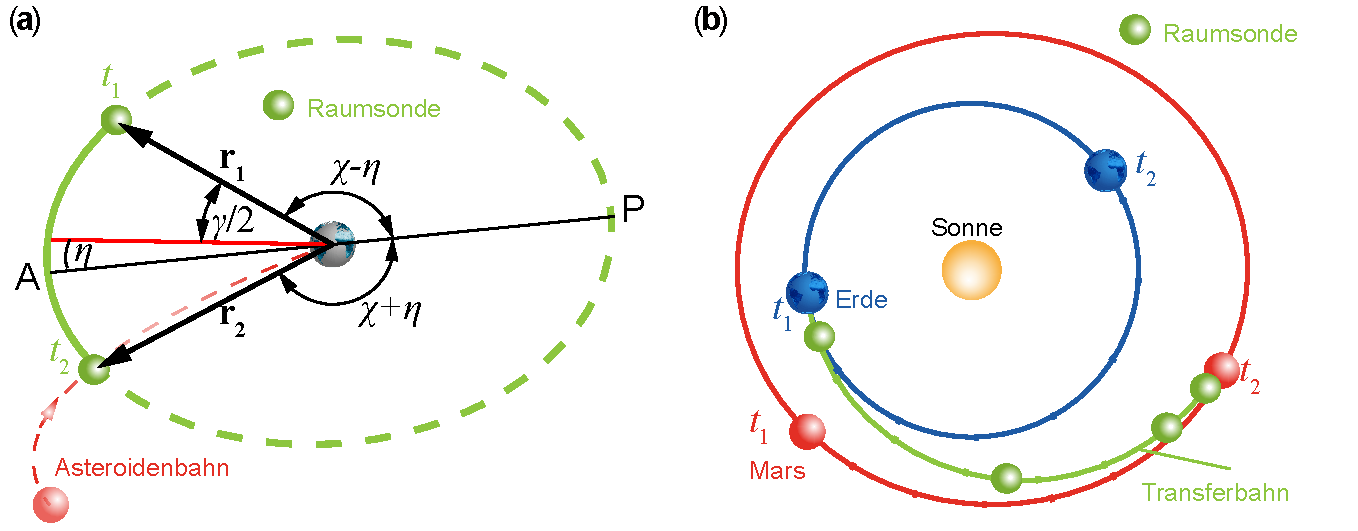
\includegraphics[width=\textwidth]{LambertProblem01Geometrie.pdf} 
	\caption[Lambert-Problem.]{\fa Geometrie des Lambert-Problems. Beispiel f�r ein Abfangen eines Asteroiden durch eine Raumsonde. \fb Anwendung des Lambert-Problems beim interplanetaren Flug zum Mars. Die Transferellipse zum Mars (Startzeitpunkt $t_1$ muss die Marsbahn zum Zeitpunkt $t_2$ auch genau dann schneiden/ber�hren, wenn der Mars sich an der entsprechenden Stelle befindet.}
	\label{abb:adyn_lambert_basic}
\end{figure}

In \figref{adyn_lambert_basic}a haben wir als Beispiel das Problem des "`Abfangens"' eines Asteroiden und in \figref{adyn_lambert_basic}b eine Planung eines Raumflugs zum Mars schematisch dargestellt, die wir in \probref{adyn_manoevers5} und  \probref{adyn_manoevers6} genauer behandeln wollen. Es gibt verschiedene Ans�tze zur L�sung des Lambert-Problems und noch heute erscheinen regelm��ig Originalarbeiten zu dem Thema. Im Wesentlichen geht es dabei um die (numerische) Optimierung der L�sungsverfahren und spezielle Probleme. Eine gute �bersicht �ber den aktuellen Stand findet sich f�r den interessierten Leser in \cite{Izzo2015} und \cite{sangra2021}, wobei die letztere Referenz auch explizit auf die \matlab-Modellierung eingeht.\\
Warum ist das Lambert-Problem so besonders? Gegeben sind beim Lambert-Problem wie oben ausgef�hrt, zwei Ortsvektoren $\vec{r}(t_1)$ und $\vec{r}(t_2)$ und die ToF. Gesucht sind die Bahnparameter und die Geschwindigkeiten $\dot{\vec{r}}(t_1)$ und $\dot{\vec{r}}(t_2)$ f�r die Kurve zwischen $\vec{r}(t_1)$ und $\vec{r}(t_2)$. Das ist ein sogenanntes \emph{Randwertproblem}\index{Randwertproblem|textbf}, welches wesentlich schwieriger zu l�sen ist als die bisher behandelten Anfangswertprobleme, bei denen alle Informationen zur Integration der Bewegungsgleichungen zum Anfangszeitpunkt bekannt waren. Im Gegensatz zu Anfangswertproblemen\index{Anfangswertproblem} haben Randwertprobleme nicht immer eine eindeutige L�sung. Die ausf�hrliche Behandlung von Randwertproblemen geht �ber den Umfang dieses Buches hinaus, wir empfehlen zur Vertiefung die Referenzen \cite{Arens2008, Fischer2014}.\footnote{Dem Lambert-Randwertproblem sind wir schon bei der Bestimmung der Bahnparameter aus zwei Ortsvektoren in \kap{adyn_orbits_determination_xwinkel} begegnet. Wir hatten dort lediglich die numerische Methodik angegeben, ohne auf das Randwertproblem einzugehen.} F�r das Lambert-Problem gibt es eine Reihe von L�sungsmethoden \cite{Izzo2015, sangra2021}, wir zeigen hier eine physikalisch sehr anschauliche, die auf \cite{Gatland2022} zur�ckgeht. In \probref{adyn_manoevers4} werden wir eine andere L�sungsmethode verwenden und auch auf weitere L�sungsmethoden verweisen. Wir f�hren mit Hilfe von \figref{adyn_lambert_basic} die folgenden Bezeichnungen ein:
\begin{align*}
    \gamma ~~~~~~~~ &\text{Winkel zwischen $\vec{r}_1$ und $\vec{r}_2$}\,,\\
    \chi   ~~~~~~~~ &\pi-\frac{\gamma}{2} \,,\\
    \eta   ~~~~~~~~ &\text{Winkel zwischen der Winkelhalbierenden von}~ \vec{r}_1 ~\text{und} ~\vec{r}_2~\text{und Apsidenlinie}~~ \overline{\mathrm{PA}}.
\end{align*}
Die Flugzeit $t_\text{F}^* = t_2-t_1$ ist als Bedingung vorgegeben, man muss also die Bahnparameter der Ellipse suchen. Wir w�hlen dazu den Parameter $p$ (\textit{semi-latus rectum}) und die Exzentrizit�t~$e$, k�nnten aber auch anstelle $p$ die gro�e Halbachse $a$ nehmen, wie wir es in \probref{adyn_manoevers4} tun werden. Mit den L�ngen der Ortsvektoren $r_{1,2}=\left|\vec{r}_{1,2}\right|$ schreiben wir mit Gleichung~\eqref{eq:hm_bahnglg}: 
\begin{align}
\begin{split}
    p &= r_1\,\lk 1+e\,\cos\lk\theta_1\rk\rk\, = r_1\,\lk 1+ e\cos\lk\chi-\eta\rk\rk\, \\
    &= r_1 \lk1+e\,\cos\chi\,\cos\eta + e\,\sin\chi\,\sin\eta\rk\,,
\end{split} \label{eq:adyn_lambert01}
\end{align}
\bzw
\begin{align}
\begin{split}
    p &= r_2\,\lk 1+e\,\cos\lk 2\pi - |\lk \chi+\eta\rk|\rk\rk \,\\
    &= r_2\,\lk 1+ e\,\cos\chi\,\cos\eta - e\,\sin\chi\,\sin\eta\rk\,. 
\end{split} \label{eq:adyn_lambert02}
\end{align}
Wir addieren \bzw subtrahieren $p/r_1$ und $p/r_2$ und erhalten nach kleiner Umformung
\begin{align}
    A &= \frac{\lek p/r_1 + p/r_2 -2\rek}{2\cos\chi} = e\,\cos\eta ~~~\text{\bzw}~~~
     B = \frac{\lek  p/r_1 - p/r_2 \rek}{2\sin\chi}  = e\,\sin\eta \,. \label{eq:adyn_lambert03}
\end{align}
Aus den beiden Gleichungen gewinnt man die Exzentrizit�t $e$ und den Winkel $\eta$:
\begin{align}
    e = \sqrt{A^2+B^2} ~~~\text{\bzw}~~~\eta = \upsilon_0 = \arctan \lk \frac{B}{A} \rk \,.\label{eq:adyn_lambert05}
\end{align}
Gegeben sind $r_1,r_2,\gamma$ und $\chi$. F�r $p$, das wir ja bestimmen wollen, kann ein Startwert $p^{(0)}$ angenommen werden, so dass dann mit \eqref{eq:adyn_lambert03} und \eqref{eq:adyn_lambert05} auch $e^{(0)}$ und $\eta^{(0)}$ bekannt sind und damit auch $\upsilon_1^{(0)} = \chi-\eta^{(0)}$ als Winkel (wahre Anomalie)\index{Anomalie!wahre} von $\vec{r}_1$ zur Periapsis und die entsprechende wahre Anomalie $\upsilon_2^{(0)} = 2\pi -\lk\chi+\eta^{(0)}\rk$. \\
Damit k�nnen wir nun f�r den angenommenen Startwert $p^{(0)}$ die Zeiten $t_{1,2}^{(0)}$ berechnen, indem wir die Beziehung \eqref{eq:hm_1-ecosEdE} f�r $t(E)$ ($E$ ist die exzentrische Anomalie) aus dem \kap{hm_abl_kepler} integrieren und dabei $a^{(0)} =p^{(0)}/\lk 1-\lk e^{(0)}\rk^2\rk$ benutzen. Wir erhalten: 
\begin{align}
    \sqrt{\frac{\mu}{p^3}}\,t_{1,2}^{(0)} = \frac{E_{1,2}^{(0)}-e^{(0)}\,\sin E_{1,2}^{(0)}}{\lk 1-\lk e^{(0)}\rk ^2\rk^{\frac{3}{2}}}\,. \label{eq:adyn_lambert06}
\end{align}
Wir k�nnen die exzentrische Anomalie\index{Anomalie!exzentrische} $E_{1,2}^{(0)}$ �ber \eqref{eq:hm_nu(t)_alternativ} aus 
\begin{align}
    \tan\lk\frac{E_{1,2}^{(0)}}{2}\rk = \sqrt{\frac{1-e^{(0)}}{1+e^{(0)}}}\,\tan\lk\frac{\upsilon_{1,2}}{2}\rk \label{eq:adyn_lambert07}
\end{align}
berechnen und vergleichen nun die mit dem Startwert berechnete Flugzeit $t_\text{F}^{(0)} = t_2^{(0)}-t_1^{(0)}$, die im Allgemeinen noch nicht mit der ToF $t_\text{F}^*=t_1-t_2$ �bereinstimmen wird. Ohne Beschr�nkung der Allgemeinheit wollen wir annehmen, dass $t_\text{F}^{(0)}>t_\text{F}^*$ ist.\\
Die weitere iterative Bestimmung des tats�chlichen Bahnparameters erfolgt, indem man einen zweiten Iterationsstartwert $p^{(1)}$ und w�hlt und zwar so, dass f�r das �ber \eqref{eq:adyn_lambert06} berechnete $t_\text{F}^{(1)}= t_2^{(1)}-t_1^{(1)}$ gilt: $t_\text{F}^{(1)} < t_\text{F}^*$.\footnote{Falls $t^{(0)}<t_\text{F}^*$ war, entsprechend umgekehrt!} Nun interpoliert man ein $p^{(2)}$ nach
\begin{align}
    p^{(2)} = \frac{t_\text{F}^*-t_\text{F}^{(1)}}{t_\text{F}^{(0)}-t_\text{F}^{(1)}}\,\lk p^{(0)}-p^{(1)}\rk + p^{(1)}  \label{eq:adyn_lambert09}
\end{align}
und berechnet $t_\text{F}^{(2)}$. Diese Interpolation wird so lange fortgesetzt bis $t_\text{F}^{(n)} \approx t_\text{F}^*$ ist. Die L�sung f�r einen �hnlichen Fall wie in  \figref{adyn_lambert_basic}a dargestellt haben wir f�r zwei exemplarische Parameters�tze im \mscr~ \mladynref{LambertProblem01.m} durchgerechnet (\figref{adyn_lambert_bsp}). \\
\begin{figure}[H]
	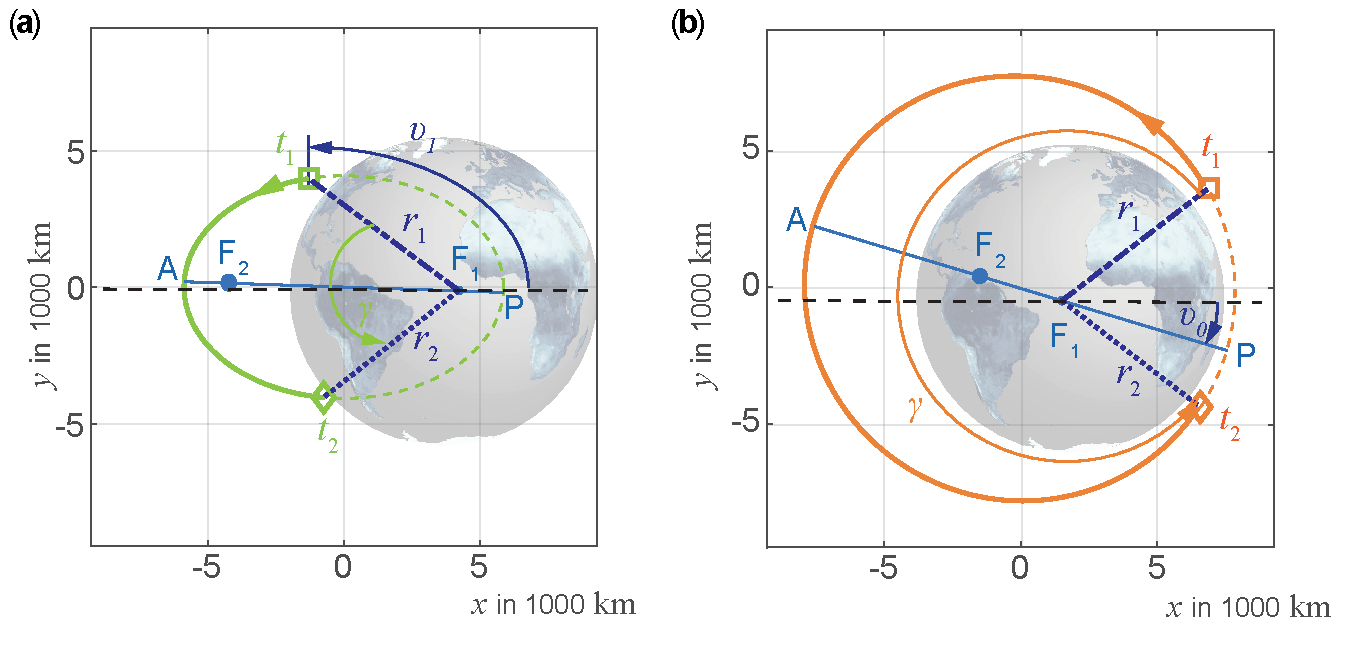
\includegraphics[width=\textwidth]{LambertProblem01Loesung.pdf} 
	\caption[L�sung des Lambert-Problems.]{L�sung des Lambert-Problems f�r das Beispiel des Abfangens einer interkontinentalen ballistischen Rakete durch eine Raumsonde im Schwerefeld der Erde. \fa Parameter: $r_1 = \SI{6800}{\kilo\metre},\, r_2 = \SI{6400}{\kilo\metre},\, \gamma=75\degree,\ t_\text{F}^*=3000s = \SI{50}{\minute}$. Es ergibt sich die gr�ne Ellipse mit Parametern $p = \SI{2831}{\kilo\metre},\, \e=0.7195,\, \eta = -1.7\degree$. \fb Mit gleichen Anfangsvektoren aber unterschiedlichem eingeschlossenen Winkel $\gamma=285\degree=360\degree- 75\degree$  ergibt sich die l�ngere orangefarbene Ellipse mit einer Flugzeit $t_\text{F}^*=6000s = \SI{100}{\minute}$ und Ellipsenparametern von: $p = \SI{7589}{\kilo\metre},\, \e=0.1988,\, \eta = -16.7\degree$. (\mscr~ \mladynref{LambertProblem01.m} nach \cite{Gatland2022}.)
	}
	\label{abb:adyn_lambert_bsp}
\end{figure}
Wir haben in der gezeigten Rechnung eine eindeutige L�sung erhalten. Das ist bei Randwertaufgaben jedoch keinesfalls immer der Fall, wie wir in \probref{adyn_manoevers4} zeigen werden. Bei ung�nstig gew�hltem Startwert $p^{(0)}$ kann es sein, dass die Itration nicht konvergiert. Es empfiehlt sich daher, sich mit einer numerischen Vorw�rtsrechnung eine Tabelle von $p^{(i)}$ und den zugeh�rigen $t_\text{F}^{(i)}$ zu beschaffen. 

F�r die Bahnberechnung in der Astrodynamik braucht man h�ufig auch die Geschwindigkeiten bei den jeweiligen normalen Anomalien, insbesondere bei $\upsilon_1$ und $\upsilon_2$. Diese berechnen sich nach \cite{Gatland2022}:
\begin{align}
    \vec{v}_\text{tr} = \sqrt{\frac{\mu}{p}}\,\lek e\,\sin\upsilon\,\vec{e}_\text{r} + \lk 1 + e \,\cos\upsilon \rk \,\vec{e}_\upsilon \rek \,,\label{eq:adyn_lambert08}
\end{align}
worin $\vec{e}_r$ \bzw $\vec{e}_\upsilon$ Einheitsvektoren sind. In \probref{adyn_manoevers4} werden wir noch eine andere Berechnung f�r die Geschwindigkeiten zeigen.\\ 
F�r das Lambert-Problem gibt es wie erw�hnt zahlreiche Anwendungen. Beispielsweise ist die Berechnung der Bahn eines Transportraumschiffs zur ISS nach dem \gls{Brennschluss} des Triebwerks der Startrakete ein Lambert-Problem, ebenso wie die Planung und Berechnung eines optimalen Startzeitpunkts (Start-Fensters) zum Mars \bzw zur Venus (\probref{adyn_manoevers5}).
In \probref{adyn_manoevers6} behandeln wir das Abfangen einer interkontinentalen ballistischen Rakete.

\subsection{Man�ver mit kontinuierlichem Schub}\label{kap:adyn_kont_maneuver}

Wir wollen uns nun Man�ver mit kontinuierlichem Schub anschauen, wie sie \zb durch Plasma- oder Ionenstrahltriebwerke oder allgemein elektrische Antriebe realisiert werden k�nnen. Diese Triebwerke sind wieder verst�rkt in das Interesse der Raumfahrt ger�ckt, beispielsweise bei der Raumsonde BepiColombo im Jahr 2018 \cite{Althaus2007, Krueger2018, Messerschmid2017}.\\
Im Gegensatz zu einem chemischen Antrieb auf Basis von Verbrennung von Treibstoff, steht beim elektrischen Antrieb quasi kontinuierlich und �ber Solarpanele auch nahezu unbegrenzt  Energie zur Verf�gung, allerdings ist die Leistung (Energie pro Zeit) begrenzt. Ein Vorteil der elektrischen Antriebe ist aber, dass die Aussto�geschwindigkeit der Teilchen (beschleunigte Ionen) mit bis zu $v_1= \SI{50}{\km\per\second}$ deutlich �ber den Werten von chemischen Triebwerken ($v_\text{G}\approx 3 \ldots 5\,\SI{}{\km\per\second}$) liegt. Damit ist pro $\SI{}{\kg}$ Treibstoffmasse auch ein etwa $10$ mal gr��erer Schub verbunden. Dennoch gibt es zwei Nachteile, 
\begin{itemize}
    \item zum einen funktionieren Ionenstrahltriebwerke nicht unter Atmosph�renbedingungen, was ihren Einsatz auf h�here Orbits und interplanetare Fl�ge begrenzt und
    \item wegen der begrenzten elektrischen Leistung sind zum anderen nur sehr kleine Sch�be im Bereich von $\SI{1e-3}{\newton}$ bis etwa $\SI{0.5}{\newton}$ m�glich. 
\end{itemize}
Damit sind auch die Einsatzbereiche der Triebwerke vorgezeichnet.\\
Wir wollen uns als ein Beispiel den Flug von einer nahen Erdumlaufbahn (\zb LEO) zu einem geostation�ren Orbit (GEO) mit einem Ionentriebwerk durch sogenanntes Aufspiralen im Vergleich zum Hohmann-Transfer (\kap{adyn_hohmann_transfer}) anschauen.
In der Bewegungsgleichung f�r kontinuierliche Sch�be soll die sich �ber die Man�verzeitdauer ver�ndernde Gravitationskraft $\vec{F}_\text{G}$ ber�cksichtigt werden. Alle anderen wirkenden Kr�fte sollen weiterhin vernachl�ssigt werden. Wir haben also f�r das Raumschiff (Masse $m_\text{R}$) mit kontinuierlichem Triebwerk folgende Bewegungsgleichung:
\begin{align}
    \ddot{\vec{r}} = \dot{\vec{v}} = \frac{\vec{F}_\text{S}\lk t\rk}{m_\text{R}(t)} +\frac{\vec{F}_\text{G}\lk\vec{r}\rk}{m_\text{R}(t)}\,.\label{eq:adyn_ionentr_01}
\end{align}
Im Allgemeinen wird man diese Gleichung nur numerisch l�sen k�nnen (\probref{adyn_manoevers7}), wir k�nnen aber mit zwei Annahmen eine gute analytische N�herung herleiten.
Es gilt zum einen, dass $|\vec{F}_\text{S}| \ll |\vec{F}_\text{G}|$ und zum anderen soll der Schub immer tangential zur Bahn, also parallel zur Geschwindigkeit erfolgen, also:
\begin{align}
    \vec{F}_\text{S}\,\vec{v}_\text{R} = F_\text{S}\,v_\text{R}\,. \label{eq:adyn_ionentr_02}
\end{align}
Das bedeutet auch, dass die Bahn w�hrend des gesamten Man�vers als kreis�hnlich betrachtet werden kann, das Aufspiralen wird also mit sehr kleinen H�hen�nderungen pro Zeit (\bzw Umlauf) verbunden sein. Man muss dann nat�rlich bei der Rechnung aufpassen, dass die Bedingungen f�r die gemachten N�herungsannahmen noch erf�llt sind. Wir benutzen die  Gleichung f�r die Gesamtenergie \eqref{eq:hm_vis-viva} und die \gls{visvivaadyn} \eqref{eq:hm_vis-viva}, die wir etwas umformen und beide nach der Zeit ableiten:
\begin{align}
\begin{split}
    \frac{\D }{\D t}\,H = \frac{\D }{\D t} \lk -\frac{\mu_\text{E}}{2a}\rk &= \frac{\D}{\D t}\lk\frac{1}{2}\,v^2 - \frac{m_\text{E}\,G}{r} \rk %= \frac{\D}{\D t} \lk\frac{1}{2}\,\vec{v}^2-\frac{\mu_\text{E}}{r}\rk 
		= \frac{\D}{\D t}\lk \frac{1}{2}\,\vec{v}^2 + U\lk r\rk \rk\\
    &=\vec{v}\,\frac{\D \vec{v}}{\D t} + \frac{\d U\lk r\rk}{\d \vec{r}}\,\frac{\D \vec{r}}{\D t}= \vec{v}\,\lk\frac{\D \vec{v}}{\D t} - \vec{g}\lk r \rk \rk \,.
\end{split} \label{eq:adyn_ionentr_03}
\end{align}
Hier haben wir die spezifische (auf die Masse bezogene) potentielle Energie 
\begin{align}
    U\lk r\rk = \frac{1}{m_\text{r}}\,\int\limits_r^\infty F_\text{G}\lk r\rk\, \D r  \label{eq:adyn_ionentr_04}
\end{align}
und die Gravitationsbeschleunigung 
\begin{align}
    \vec{g} = \frac{\vec{F}_\text{G}}{m_\text{r}} = - \frac{\d}{\d \vec{r}}\,U\lk r\rk = -\vec{\nabla}\,U\lk r\rk \label{eq:adyn_ionentr_05}
\end{align}
benutzt. 
%Gleichung \eqref{eq:adyn_ionentr_03} ist aber nach \eqref{eq:hm_bewgl1} gleich der zeitlichen Ableitung der Gesamtenergie, also:
%\begin{align}
    %\frac{\D }{\D t} = \lk -\frac{\mu_\text{E}}{2a}\rk = \frac{\D }{\D t}\,H\,. \label{eq:adyn_ionentr_06}
%\end{align}
Damit k�nnen wir \eqref{eq:adyn_ionentr_03} mit \eqref{eq:adyn_ionentr_01} schreiben:
\begin{align}
    \frac{\D}{\D t}\, H = \vec{v}\,\lk \frac{\vec{F}_\text{S}}{m_\text{R}} + \vec{g} - \vec{g} \rk = \vec{v}\,\frac{\vec{F}_\text{S}}{m_\text{R}} ~~~~ \rightarrow ~~~~ \frac{1}{v}\,\frac{\D}{\D t}\,H = \frac{F_\text{S}}{m_\text{R}}\,.\label{eq:adyn_ionentr_07}
\end{align}
Das ist unsere Bewegungsgleichung. Die bereits gemachte Annahme f�r kleine Sch�be f�hrt zu kreis�hnlichen Bahnen, die wir durch
\begin{align}
    v = \left|r \dot{\varphi} \vec{e}_\varphi \right| = \sqrt{\frac{G\,m_\text{E}}{r}} = \sqrt{\frac{\mu_\text{E}}{r}}~~~~ \text{und} ~~~~ H =-\frac{G\,m_\text{E}}{2r}= -\frac{\mu_\text{E}}{2r} \label{eq:adyn_ionentr_08}
\end{align}
ausdr�cken (siehe auch \kap{hm_abl_kepler}). \\
Damit erhalten wir:
\begin{align*}
    \frac{1}{2}\,\sqrt{\frac{\mu_\text{E}}{r^3}}\,\frac{\D r}{\D t} = \frac{F_\text{S}}{m_\text{R}}
\end{align*}
und durch Integration
\begin{align}
\begin{split}
    \frac{\sqrt{\mu_\text{E}}}{2}\,\int\nolimits_{r_1\approx R_\text{E}+h}^{r_2} r^{-\frac{3}{2}}\,\D r = &-\sqrt{\mu_\text{E}}\,\lk \frac{1}{\sqrt{r_2}} - \frac{1}{\sqrt{r_1}}\rk = \int\nolimits_{t=0}^{t_\text{end}}\,\frac{F_\text{S}}{m_\text{R}}\,\D t = \Delta v_\text{kont}\\
    \rightarrow ~~~~ &\Delta v_\text{kont} = \sqrt{\frac{\mu_\text{E}}{r_1}}\,\lk 1-\sqrt{\frac{r_1}{r_2}}\rk = v_1-v_2 \,.
\end{split} \, \label{eq:adyn_ionentr_09}
\end{align}
Beim kontinuierlichen Schub ist also der Geschwindigkeitsbedarf durch die Differenz der Umlaufgeschwindigkeiten in der Anfangs- und Endbahn gegeben. \\
Vergleichen wir das mit dem Hohmann-Transfer \eqref{eq:adyn_hohmann04}
\begin{align}
    \Delta v_\text{Hohmann}=  v_\text{P}-v_\text{A} +v_2-v_1 = v_\text{P}-v_\text{A} -\Delta v_\text{kont}\,, \label{eq:adyn_ionentr_10}
\end{align}
so sehen wir, dass beim kontinuierlichen Schub ein h�herer Energiebetrag notwendig ist (\figref{adyn_Ionenantrieb01}a). \\
Wir wollen noch die Flugzeit unter der Annahme konstanten Schubs und konstanter Massenverlustrate $\dot{m}_\text{R}$ (das sind im wesentlichen die ausgesto�enen Ionen) berechnen. Aus \eqref{eq:adyn_ionentr_07} folgt dann mit $m\lk t\rk = m_0 - \dot{m}_\text{r}\lk t-t_0\rk$:
\begin{align*}
    \int\limits_{t_0}^t\frac{F_\text{S}}{m\lk t \rk} \,\D t = \frac{F_\text{S}}{m_0}\,\int\limits_{t_0}^t \, \frac{\D t'}{1-\frac{\dot{m}_\text{R}}{m_0}\,\lk t'-t_0 \rk} = \frac{F_\text{S}}{\dot{m}_\text{R}} \,\ln \,\lek 1-\frac{\dot{m}_\text{R}}{m_0}\,\lk t-t_0\rk\rek
\end{align*}
\begin{align*}
    \rightarrow ~~~~ \frac{r}{r_1} = \lek 1 + \sqrt{\frac{r_1}{\mu_\text{E}}}\,\frac{F_\text{S}}{\dot{m}_\text{R}}\,\lk \ln \lek 1-\frac{\dot{m}_\text{R}}{m_0}\,\lk t-t_0\rk\rek\rk\rek \;. 
\end{align*}
Wir haben die Zeiten f�r den Flug zum GEO mit kontinuierlichem Antrieb in \figref{adyn_Ionenantrieb02} dargestellt und mit denen f�r einen �quivalenten Hohmann-Transfer verglichen.
Man erkennt, dass bei kontinuierlichen (elektrischen) Triebwerken mit deutlich l�ngeren Flugzeiten zu rechnen ist. Deswegen kommt es bei Raketenantrieben immer zu einer Kombination von chemischen Triebwerken (schon f�r den Start von der Erde notwendig) und elektrischen Triebwerken. Wir wollen nochmals explizit darauf hinweisen, dass die N�herungsannahmen, die wir weiter oben gemacht haben, nicht mehr f�r die gesamte Flugzeit erf�llt sind. Das kann man auch am starken Anstieg der Kurve $r(t)$ am Ende der Flugzeit sehen. Eine detaillierte numerische Rechnung ist Gegenstand von \probref{adyn_manoevers7}. In \probref{adyn_manoevers8} wollen wir dann auch den Flug mit einem kontinuierlichen Antrieb zum Mars aus einer Parkbahn um den Mond heraus betrachten und die Gleichung \eqref{eq:adyn_ionentr_01} numerisch l�sen. Es sei darauf hingewiesen, dass auch der Strahlungsdruck (siehe \kap{adyn_strahlungsdruck}) besonders im interplanetaren Raum zum kontinuierlichen Antrieb benutzt werden. Dazu werden Raumschiffe mit sogenannte Sonnensegeln ausgestattet. In \cite{Bailer2021} wird die japanische Mission IKAROS behandelt, die mit einem solchen Antrieb im interplanetaren Raum unterwegs ist. 

\begin{figure}[H]
	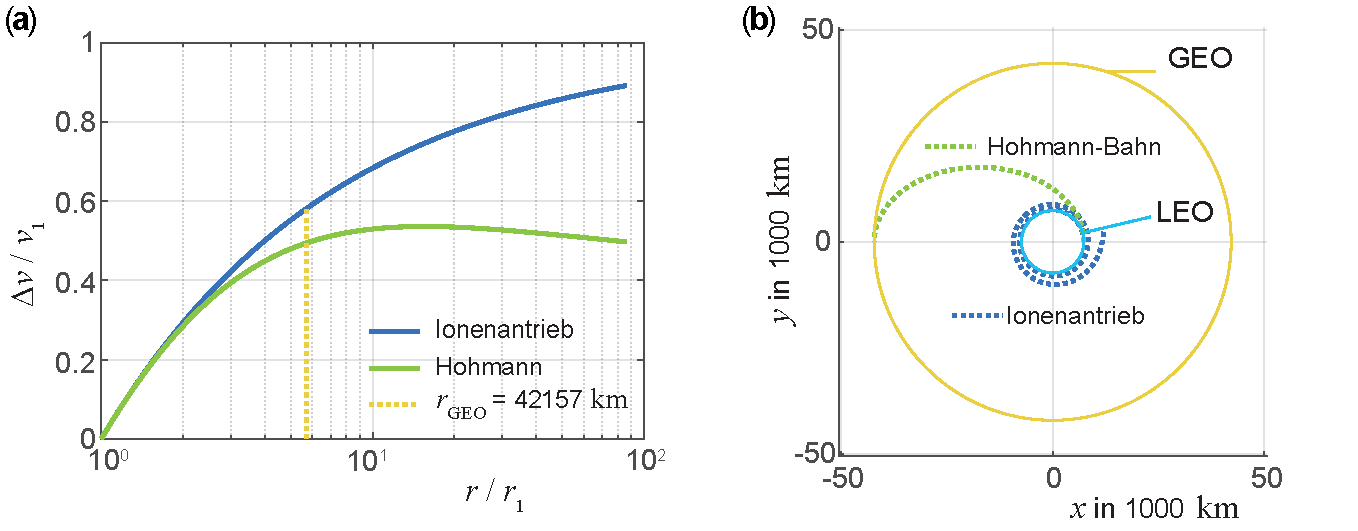
\includegraphics[width=\textwidth]{Ionenantrieb01.pdf} 
	\caption[Ionenantrieb im Vergleich zu Hohmann-Transfer.]{Ionenantrieb im Vergleich zu einem Hohmann-Transfer. \fa Geschwindigkeitsbedarf f�r Transfer von $r_1$ nach $r_2$. \fb Bahnform. Parameter: $r_1= \SI{1000}{\km} + R_\text{E}$, $r_2 = \SI{35786}{\km} + R_\text{E}$, Schub $F_\text{S}= \SI{0.5}{\newton}$, Anfangsmasse $m_0= \SI{10000}{\kg}$, Massenaussto� $\dot{m}_\text{R} = \SI{3e-3}{\kg\per\second}$. }
	\label{abb:adyn_Ionenantrieb01}
\end{figure}

\begin{figure}[H]
	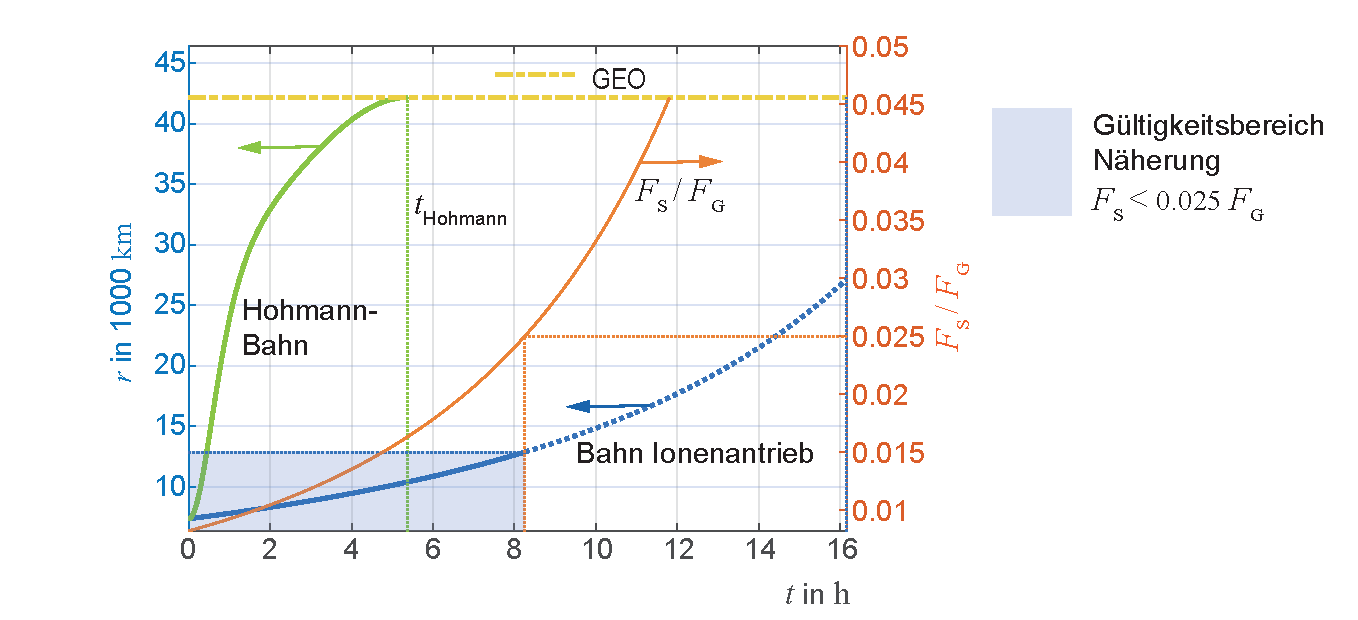
\includegraphics[width=\textwidth]{Ionenantrieb02.pdf} 
	\caption[Abstand zur Erde und Flugzeit bei Flug zu geostation�rem Orbit.]{Abstand zur Erde und Flugzeit bei einem Flug zu einem geostation�ren Orbit mit Ionenantrieb im Vergleich zu einem Hohmann-Transfer.}
	\label{abb:adyn_Ionenantrieb02}
\end{figure}


\subsection{Gravity-Assist-Man�ver}\label{kap:adyn_gravity_assist}

Wir wollen nun die ebenfalls sehr wichtigen \glslink{GA}{\textit{Gravity-Assist-Man�ver (GA-Man�ver)}}\index{Gravity-Assist-Man�ver} behandeln, denen wir bereits unter dem Namen Swing-By\index{Swing-By-Man�ver}\footnote{Wir benutzen die Begriffe GA-Man�ver und Swing-By-Man�ver synonym. H�ufig wird auch die Schreibweise Swingby oder Flyby verwendet.} im Kapitel 1 von Band I und auch im Kapitel Himmelsmechanik begegnet sind. 
Warum ist das Gravity-Assist-Man�ver f�r die Raumfahrt insbesondere zu den weiter entfernten Planeten so bedeutsam? Der Hohmann-Transfer erfordert bei entfernt liegenden Planeten sehr gro�e Geschwindigkeitsbudgets und f�hrt auch zu sehr langen Flugzeiten. So br�uchte man nach \eqref{eq:adyn_hohmann04} f�r einen Hohmann-Transfer zum Jupiter bereits ein $\Delta v \approx \SI{14}{\km\per\second}$, was zumindest bei der derzeitigen Raketentechnologie zu v�llig unakzeptablen, \dh verschwindenden, Nutzlasten f�hren w�rde.\\ 

\begin{figure}[H]
	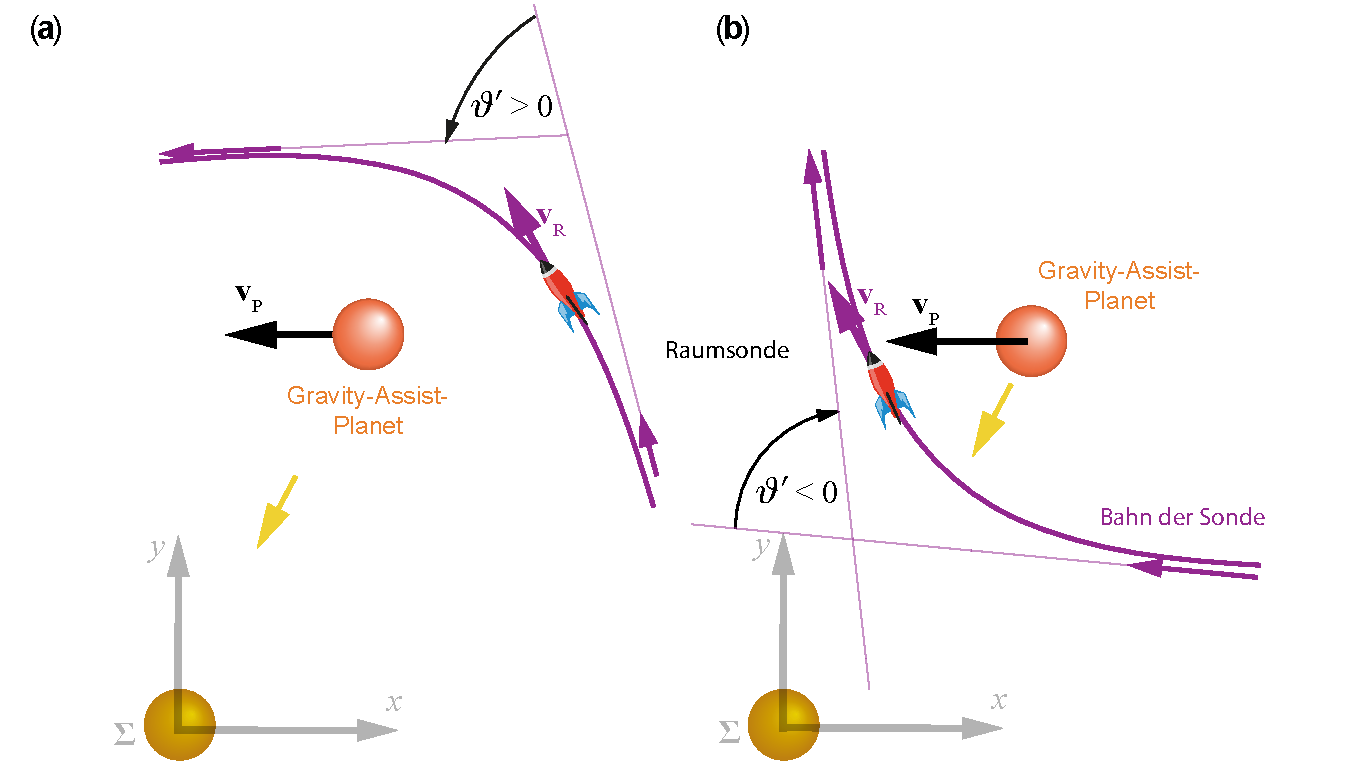
\includegraphics[width=\textwidth]{GravityAssistManoever01.pdf} 
	\caption[Verschiedene Swing-By-Man�ver im heliozentrischen \KOS .]{Swing-By-Man�ver im heliozentrischen Koordinatensystem. \fa Bahn der Sonde liegt "`hinter"' dem Planeten, die Ablenkung erfolgt entgegen dem Uhrzeigersinn ($\vartheta' >0$). \fb Bahn der Sonde liegt "`vor"' dem Planeten, die Ablenkung erfolgt im Uhrzeigersinn ($\vartheta' < 0$).}
	\label{abb:adyn_swingby00}
\end{figure}

Erst mit den Swing-By-Man�vern wurden solche interplanetaren Raumfl�ge wirklich m�glich. Erw�hnenswert ist, dass die Entdeckung des Swing-By 1961 von dem Mathematik-Studenten Michael Minovitch\footnote{Michael Minovitch (geb. 1935) ist ein US-amerikanischer Mathematiker, der als erster gezeigt hat, dass die Bahnen von Raumsonden beim Vorbeiflug an Planeten durch ein Swing-By-Man�ver Geschwindigkeit hinzugewinnen k�nnen.}\indexp{Minovitch, Michael Andrew} w�hrend seines studentischen Praktikums am \textit{\gls{jpladyn}~(JPL)}\index{Jet Propulsion Lab (JPL)} in Pasadena (Kalifornien) gemacht wurde. Innerhalb der NASA und der ESA wird auch Giuseppe Colombo\footnote{Giuseppe Colombo (1920--1984) war ein italienischer Ingenieur und Mathematiker, der auf den Gebieten der theoretischer Mechanik, insbesondere der Schwingungs- und Himmelsmechanik und der Astrodynamik t�tig war. Neben seinen Beitr�gen zum Swing-By ist auch seine Konzeptentwicklung des Space Tethers (Weltraumfahrstuhl, siehe auch �bung im Kapitel 1, Band I)\indexp{Colombo, Giuseppe} erw�hnenswert.} als konzeptioneller Kopf und genialer Weiterentwickler von Swing-By-Man�vern genannt.\\
Wie kann eine Raumsonde durch ein GA-Man�ver an einem Planeten an Geschwindigkeit gewinnen? Wir hatten im Kapitel Streuprobleme (Band I, Kapitel  1.3.5) gesehen, dass es sich bei Swing-By-Man�vern um ein elastisches Streuproblem im Gravitationsfeld des Planeten handelt. Die Bewegung einer Sonde um den sogenannten Gravity-Assist-Planeten erfolgt auf einer Hyperbelbahn und nat�rlich bleibt bei diesem elastischen Streuprozess die Gesamtenergie des Systems erhalten. Es findet aber eine Energie�bertragung $\Delta T$ zwischen Planet und Raumsonde statt, die im heliozentrischen \KOS\ zu einer Geschwindigkeits�nderung der Sonde f�hrt. Das GA-Man�ver ist im reinen Zweik�rperproblem nicht erkl�rbar, denn es muss die heliozentrische Geschwindigkeit des Planeten f�r die Erkl�rung des Energie- \bzw Geschwindigkeits�bertrags ber�cksichtigt werden.\footnote{In der Referenz \cite{Walter2018} wird eine sch�ne Analogie f�r den Swing-By gegeben. Nach dieser kann eine Raumsonde mit einem Roller-Skater verglichen werden. Der Roller-Skater h�ngt sich f�r eine kurze Zeit an einem vorbeifahrenden Bus (den Planeten), l�sst diesen dann nach einiger Zeit wieder los und hat damit Geschwindigkeit gewonnen. Das Festhalten entspricht der Gravitationskraft zwischen Planet und Raumsonde.} Man behandelt deshalb das Problem des Swing-By in einer Abfolge von Schritten, zun�chst im heliozentrischen, dann im planetaren und zum Schluss wieder im heliozentrischen System, in dem dann ja auch der Geschwindigkeitsgewinn beobachtet wird.\\

\begin{figure}[H]
	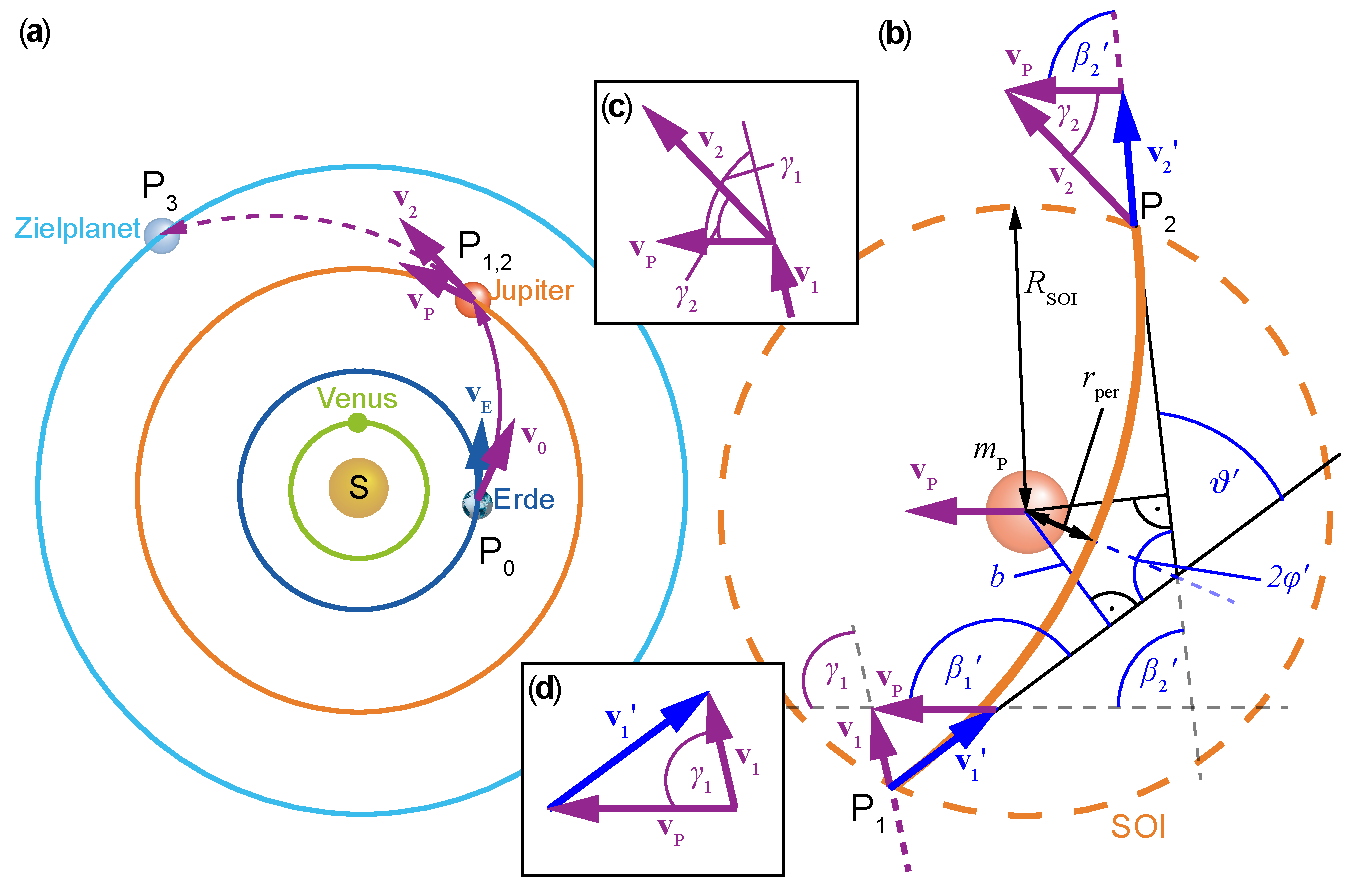
\includegraphics[width=\textwidth]{SwingByHeliozPlanetoz.pdf} 
	\caption[Swing-By-Man�ver im heliozentrischen und planetaren \KOS .]{Swing-By-Man�ver im heliozentrischen \fa und im planetaren \KOS\ \fb im Bereich der Einflusssph�re (SOI). Wir haben hierbei auch f�r die weiteren Darstellungen folgende Konventionen gew�hlt: Gr��en im heliozentrischen \KOS\ sind ungestrichen (\zb $\vec{v}_1,\, \gamma_1$) und in der Farbe lila dargestellt, w�hrend Gr��en im planetaren \KOS\ dagegen gestrichen (\zb $\vec{v}_1{}',\,\beta_1{}'$) und in den Farben blau oder orange angegeben sind. Systemunabh�ngige Gr��en sind ungestrichen (\zb $r_\text{per},\, R_\text{SOI}$) und in der Farbe schwarz dargestellt. Die Inlets zeigen \fc die Geschwindigkeitsverh�ltnisse am Eintrittspunkt in die SOI des Planeten \bzw \fd die Gesamt�nderung des heliozentrischen Geschwindigkeitsvektors der Raumsonde.}
	\label{abb:adyn_swingby01}
\end{figure}

Wir wollen uns die mathematische Behandlung des Swing-By-Man�vers etwas vereinfachen, indem wir annehmen, dass alle Bewegungen in der Ebene der Ekliptik stattfinden. 
Bei der Streuung am Planeten wird die Raumsonde um einen zun�chst noch nicht bekannten Winkel $\vartheta'$ abgelenkt. Dabei kann der Winkel sowohl negativ (Richtungs�nderung entgegen dem Uhrzeigersinn) als auch positiv (Richtungs�nderung im Uhrzeigersinn) sein, siehe \figref{adyn_swingby00}, je nachdem, ob sich die Sonde "`vor"' oder "`hinter"' dem Planeten (von der Sonne aus betrachtet) an diesem vorbei bewegt. Gleiches gilt f�r die Geschwindigkeits�nderung.\\ 
\figref{adyn_swingby01}a zeigt das Gravity-Assist-Man�ver im heliozentrischen \KOS\ und \figref{adyn_swingby01}b im \KOS\ des Gravity-Assist-Planeten, welches wegen der gro�en Masse $m_\text{P} \gg m_\text{R}$ zugleich das Schwerpunktsystem ist. Mit den Bezeichnungen aus den Abbildungen finden wir f�r die Situation am Punkt $\text{P}_1$ vor dem Swing-By-Man�ver, \dh vor der Streuung (\figref{adyn_swingby01}c):
\begin{subequations}
    \begin{align}
        \vec{v}_1{}' &= \vec{v}_1 - \vec{v}_\text{P}\,, \label{eq:adyn_swingby01a} \\
        {v_1{}'}^2 &= v_1{}^2 + v_\text{P}{}^2 - 2\,v_1\,v_\text{P}\,\cos\gamma_1\,.\label{eq:adyn_swingby01b} 
    \end{align} \label{eq:adyn_swingby01} 
\end{subequations}
Hierbei haben wir unterstellt, dass wir in der sogenannten \gls{SOI} (englisch \textit{Sphere of Influence} (SOI))\index{Einflusssph�re}\index{Sphere of Influence (SOI)} des Gravity-Assist-Planeten (in \figref{adyn_swingby01}b als gestrichelter Kreis gezeichnet) nur die Gravitationskraft des Gravity-Assist-Planeten ber�cksichtigen m�ssen\footnote{Die Berechnung der Gr��e der \gls{SOI} (SOI) ist nicht ganz einfach, h�ufig finden sich in der Literatur auch nicht ganz korrekte Definitionen und Berechnungen f�r die SOI. Wir geben die Werte f�r die Radien der SOI der einzelnen Planeten am Ende dieses Kapitels in Tabelle \ref{tab:adyn_results_swingby} an und empfehlen \probref{adyn_SOI}, in der wir die korrekte Beziehung herleiten.}.

\begin{figure}[H]
	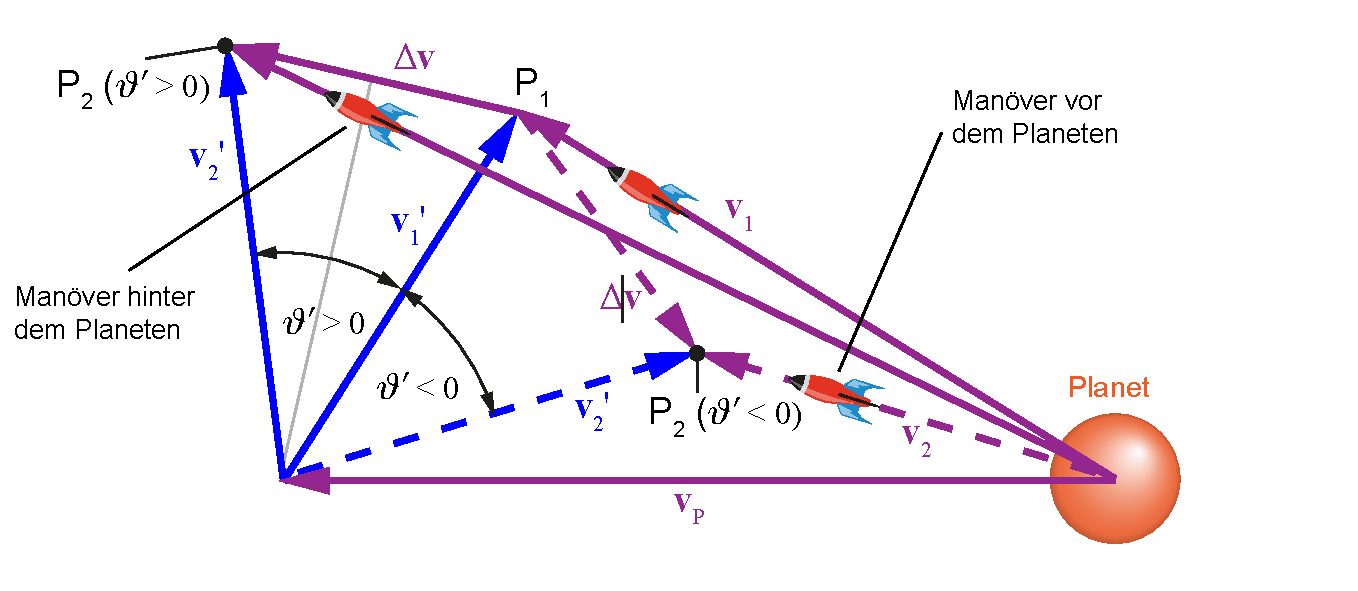
\includegraphics[width=\textwidth]{FlyByVorHinterPlanet.pdf} 
	\caption[Vektordiagramm der Geschwindigkeiten beim Swing-By-Man�ver.]{Vektordiagramm der Geschwindigkeiten beim Swing-By-Man�ver. Die Darstellung ist eine Kombination der beiden Teilzeichnungen \figref{adyn_swingby01}c,d f�r die jeweiligen F�lle des GA-Man�vers "`vor"' \bzw "`hinter"' dem Planeten.}
	\label{abb:adyn_swingby01a}
\end{figure}

Wegen Energieerhaltung beim elastischen Sto� gilt
\begin{align}
    v_1{}' = v_2{}' = v_\infty{} \,, \label{eq:adyn_swingby02} 
\end{align}
worin wir die asymptotische Geschwindigkeit in der Streuhyperbel mit $ v_\infty{}$ bezeichnet haben. Au�erhalb der SOI wird der Einfluss der Gravitation des Planeten gegen�ber der Gravitation der Sonne vernachl�ssigt, so dass am Punkt $\text{P}_2$ (\vgl \figref{adyn_swingby00}b) f�r die Geschwindigkeit $\vec{v}_2$ dann im heliozentrischen System wieder gilt:
\begin{subequations}
    \begin{align}
        \vec{v}_2 &= \vec{v}_2{}' + \vec{v}_\text{P} \,, \label{eq:adyn_swingby03a} \\
        v_2{}^2 &= {v_\infty{}}^2 + v_\text{P}{}^2 - 2\,v_\infty{}\,v_\text{P}\,\cos(180\degree - \beta_2{}') = {v_\infty{}}^2 + v_\text{P}{}^2 + 2\,v_\infty{}\,v_\text{P}\,\cos\beta_2{}'\,. \label{eq:adyn_swingby03b} 
    \end{align} \label{eq:adyn_swingby03} 
\end{subequations}
Man erkennt schon an den Gleichungen \eqref{eq:adyn_swingby01b} und \eqref{eq:adyn_swingby03b}, dass ein Geschwindigkeitsgewinn $\Delta v = v_2-v_1$ mit der Geschwindigkeit der Bewegung des Gravity-Assist-Planeten $v_\text{P}$ zusammenh�ngt. Dies ist in \figref{adyn_swingby01a} f�r die beiden F�lle $\vartheta' >0$ und $\vartheta' <0$ verdeutlicht.\\
Wir wollen nun diesen Geschwindigkeitsgewinn nach folgendem Schema berechnen:
\begin{enumerate}[1.]
	\item \textit{Berechnung der Anflugbedingungen im heliozentrischen System}\\ 

	Die als bekannt angenommenen Anflugbedingungen sind die heliozentrische Geschwindigkeit der Raumsonde $\vec{v}_1$, die Bahngeschwindigkeit $\vec{v}_\text{P}$ des Planeten, dessen Masse $m_\text{P}$ und der kleinste Abstand $r_\text{per}$ (periplanetarer Abstand), den die Raumsonde im Vorbeiflug am Planeten erreichen kann. Letzterer entspricht dem Perizentrumsabstand\index{Perizentrum} der Streuhyperbel. Dar�ber hinaus seien noch die Vektoren $\vec{r}_\text{R}$ und $\vec{r}_\text{P}$ bekannt.
	Aus den Vektorwerten $\vec{v}_1$ und $\vec{v}_\text{P}$ berechnen sich die Betr�ge $v_1,\,v_\text{P}$ und der Winkel $\gamma_1{}$.\\
	
	\item \textit{�bergang ins planetare System und Berechnung des Streuwinkels}\\ 
	
	�ber Gleichung \eqref{eq:adyn_swingby01} berechnet man $v_1{}'=v_\infty{}$ und $\gamma_1{}$. 
	Nun muss der Streuwinkel~$\vartheta'$ bestimmt werden. % f�r den nach \figref{adyn_swingby01} die Beziehung $\vartheta' = 180\degree-2\varphi'$ gilt. 
	Hier k�nnen  die Ergebnisse aus der Behandlung der Rutherford-Streuung\index{Streuung,!Rutherford-} im Kapitel Streuprobleme (Band I, Kapitel  1.3.5) benutzt werden, da wegen $m_\text{P} \gg m_\text{R}$ das planetare System auch gleichzeitig das Schwerpunktsystem f�r die Streuung der Raumsonde am Planeten ist. Den Streuwinkel f�r das Zentralkraftfeld hatte wir dort mit Formel (1.80) wie folgt berechnet:
	\begin{align}
		\sin^2\lk \frac{\vartheta'}{2} \rk & \:=\: \frac{1}{1 + 4 E^2 b^2/\alpha^2}\,, \label{eq:adyn_StreuungVglBew}
	\end{align}
	worin $E$ die Energie des einfallenden Streuteilchens, $\alpha$ die St�rke des Zentralkraftfeldes (dort war es ein Coulomb-Feld) und $b$ der Streuparameter waren. Nun m�ssen die �quivalenten Gr��en f�r das Swing-By-Man�vers im Gravitationsfeld berechnet werden.
	Da hier mit auf die Masse der Raumsonde bezogenen Gr��en gerechnet wird, ergibt sich mit der Masse $m_\text{P}$ des Gravity-Assist-Planeten f�r die Energie $H$ \bzw $\alpha$ :
	\begin{align}
	\begin{split}
 		H &= \frac{v_\infty{}^2}{2} ~~~~ (\text{f�r} ~~~~ r\to \infty \,~~~ \text{vgl.}~\eqref{eq:hm_bewgl1})\,, \\ 
		\alpha &= G\,m_\text{P}=\mu_\text{P}\,. 
	\end{split} \label{eq:adyn_swingby09a}
	\end{align}
Der Streuparameter $b$, der sich durch die Geschwindigkeit $\vec{v}_1$ und damit auch den Winkel $\gamma_1$ aus der Flugsteuerung am Punkt $\text{P}_0$ aus der Erdumlaufbahn bestimmt, h�ngt mit dem Drehimpuls �ber 
\begin{align}
    L_\infty &= b\,v_\infty  \label{eq:adyn_swingby09b} 
\end{align}
zusammen. Man ersetzt den Drehimpuls $L_\infty$ durch den Drehimpuls $L_{r_\text{per}} = r_\text{per}\,v_\text{max}{}'$ am Perizentrumsabstand der Bahn (Es gilt Drehimpulserhaltung!) und benutzt dabei den vis-viva-Satz\index{vis-viva-Satz} \eqref{eq:hm_vis-viva}:
\begin{align}
\begin{split}
    L_\infty &= b\,v_\infty{} = r_\text{per}\,v_\text{max}{}'~~~\rightarrow~~~ b= r_\text{per}\,\frac{v_\text{max}{}'}{v_\infty{}} \\
		\rightarrow~~\frac{v_\infty{}^2}{2} &= \frac{v_\text{max}{}'^2}{2} - \frac{\mu_\text{P}}{r_\text{per}} \\
		\rightarrow~~v_\text{max}{}' &= v_\infty{}\,\sqrt{1+\frac{\tilde{v}_\text{F}{}^2}{v_\infty{}^2}}\,.
	\end{split} \label{eq:adyn_swingby10}
\end{align}
Die \gls{vescape} vom Perizentrum (Punkt des minimalen Abstandes der Sondenbahn zum Planeten) $\tilde{v}_\text{F}$ wurde hier als
 \begin{align}
    \tilde{v}_\text{F} &= \sqrt{\frac{2\mu_\text{P}}{r_\text{per}}}\, \label{eq:adyn_swingby09c} 
\end{align}
definiert und ist durch die Masse des Planeten $m_\text{P}$ und den periplanetaren Abstand $r_\text{per}$ vollst�ndig bestimmt. Setzt man noch \eqref{eq:adyn_swingby09a}, $b$ aus \eqref{eq:adyn_swingby10} und $\tilde{v}_\text{F}$ aus \eqref {eq:adyn_swingby09c} in \eqref{eq:adyn_StreuungVglBew} ein, erh�lt man f�r den Streuwinkel die relativ einfache Beziehung
	\begin{align}
		\sin\lk \frac{\left|\vartheta'\right|}{2} \rk & \:=\: \frac{1}{1 + 2\,\lk v_\infty{}^2/\tilde{v}_\text{F}{}^2\rk}\,. \label{eq:adyn_Streuung13b}
	\end{align}

In \eqref{eq:adyn_Streuung13b} ist Betrag des Streuwinkels $\vartheta'$ enthalten, was bedeutet, dass dieser positiv oder negativ sein.\footnote{In \probref{adyn_swingby04} werden wir genauer untersuchen, unter welchen Bedingungen $\vartheta' > 0$ \bzw $\vartheta' < 0$ wird. Ebenso betrachten wir dort den Fall, dass die Bahnebene der Raumsonde und die Planetenebene nicht mehr �bereinstimmen und die Bahnebene auch nicht mehr der Ekliptik\index{Ekliptik} entspricht.} Wir arbeiten mit $\vartheta' > 0$ weiter und erhalten aus \eqref{eq:adyn_Streuung13b} und \figref{adyn_swingby01a} sofort die Geschwindigkeitsdifferenz $\Delta v'$:
	\begin{align}
		\sin\lk \frac{\left|\vartheta'\right|}{2} \rk & \:=\: \frac{\left|\Delta \vec{v}'\right|/2}{\left|\vec{v}_1{}'\right|} = \frac{\Delta v'}{v_\infty{}} = \frac{1}{1 + 2\,\lk v_\infty{}^2/\tilde{v}_\text{F}{}^2\rk} \,. \label{eq:adyn_Streuung13c} 
	\end{align}

	\item \textit{�bergang zur�ck ins heliozentrische System und Berechnung des Geschwindigkeitsvektors der Raumsonde beim Verlassen der Einflusssph�re des Planeten}\\ 

Man kann sich zun�chst leicht �berlegen, dass der Betrag der Geschwindigkeits�nderung $\Delta \vec{v}'$ in beiden Koordinatensystemen gleich gro� ist.
F�r den Vektor der Geschwindigkeit $\vec{v}_2{}'$ gilt im planetaren System (\vgl \figref{adyn_swingby01}a und \figref{adyn_swingby01a}):
	\begin{align}
		\vec{v}_2{}'& \:=\: \mathbb{R}_z(-\vartheta')\,\,\vec{v}_1{}' = \begin{pmatrix} \cos \vartheta' & -\sin \vartheta'\\ \sin \vartheta' & \cos \vartheta' \end{pmatrix}\,\, \vec{v}_1{}'
		\,. \label{eq:adyn_swingby_result01}
	\end{align}
Im heliozentrischen System ergibt sich mit \eqref{eq:adyn_swingby01a} und \eqref{eq:adyn_swingby03a} f�r den Vektor der Geschwindigkeit $\vec{v}_2{}$:
	\begin{align}
		\vec{v}_2{}& \:=\: \mathbb{R}_z(-\vartheta')\,\lk \vec{v}_1{} - \vec{v}_\text{P} \rk + \vec{v}_\text{P} \,. \label{eq:adyn_swingby_result01a}
	\end{align}
Auf Grund des Oberth-Effektes\index{Oberth-Effekt} kann man noch ein zus�tzliches $\Delta v_\text{ext}$ zu $\vec{v}_2 - \vec{v}_1$ erzielen, wenn beim Durchlaufen des minimalen Perizentrumsabstands ein Burn erfolgt. Wir wollen das im Detail in \probref{adyn_swingby02} untersuchen. Eine Simulation des Swing-By komplett im heliozentrischen \KOS\ findet sich in \probref{adyn_swingby03}. 
\end{enumerate}

Wir wollen Gleichungen \eqref{eq:adyn_swingby_result01} und \eqref{eq:adyn_swingby_result01a} auswerten. Man erkennt, dass die Ausgangswerte eines Swing-By-Man�vers nur von dem Verh�ltnis $v_\infty{}^2/\tilde{v}_\text{F}{}^2$ abh�ngen, je kleiner dieses Verh�ltnis ist, um so gr��er wird $\Delta v$ und $\vartheta'$ und umgekehrt. Man erkennt ferner, dass
\begin{itemize}
    \item $\Delta v$ sowohl gr��er als auch kleiner als Null sein kann, also zu einer Beschleunigung oder zu einem Abbremsen der Raumsonde f�hrt, je nach $\gamma_1$ \bzw $\vartheta_1'$, \dh Vorbeiflug \anf{vor} oder \anf{hinter} dem Planeten,
    \item je kleiner $r_\text{per}$ ist, \dh je dichter am Planeten des Gravity-Assist-Man�ver erfolgt, desto gr��er auch $|\Delta v|$ und $|\vartheta'|$ sind, und   
    \item offensichtlich je gr��er $m_\text{P}$ und $v_\text{P}$ sind, desto gr��er auch $|\Delta v|$ und $|\vartheta'|$ sind.
\end{itemize}

\begin{figure}[H]
	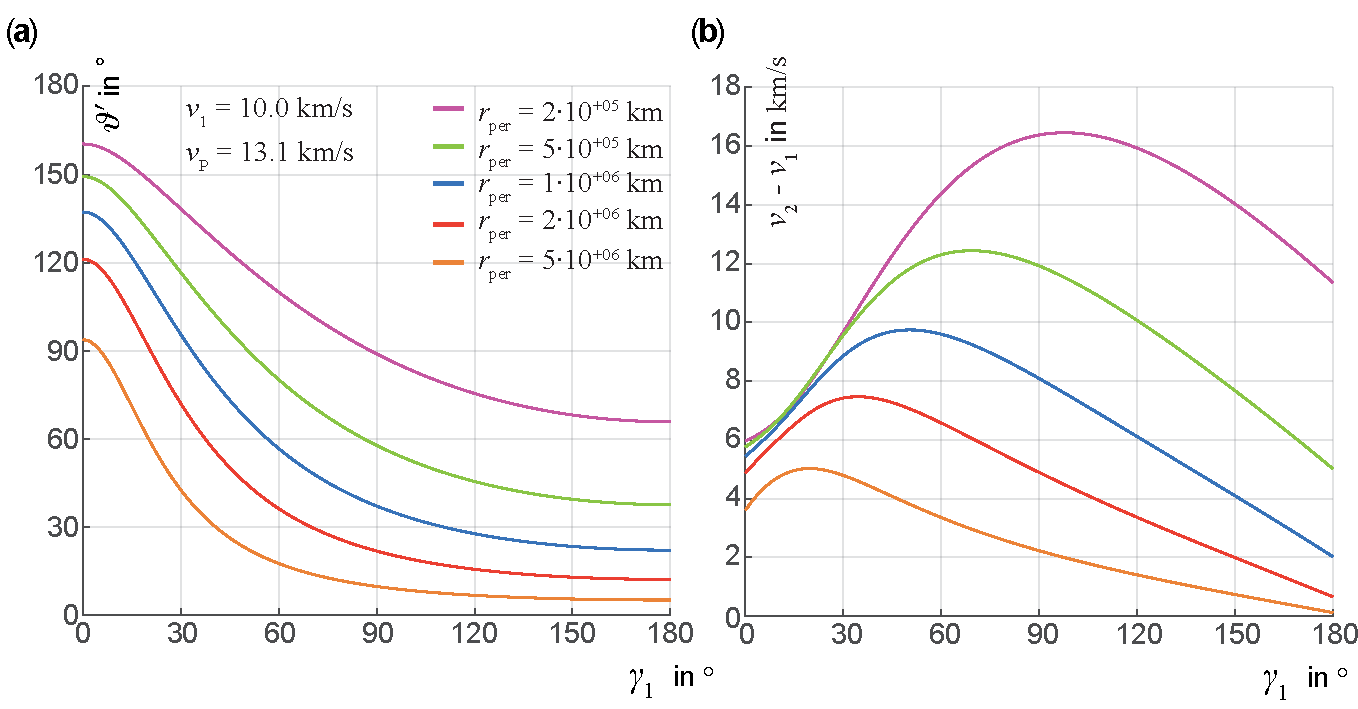
\includegraphics[width=\textwidth]{SwingByJupiter.pdf} 
	\caption[Swing-By-Man�ver am Jupiter.]{Swing-By-Man�ver am Jupiter.  \fa Streuwinkel $\vartheta'$  \fb Geschwindigkeitsgewinn $\vec{v}_2 - \vec{v}_1$ f�r verschiedene periplanetare Abst�nde $r_\text{per}$ als Funktion des Winkels $\gamma_1$.}
	\label{abb:adyn_swingby02}
\end{figure}

\begin{figure}[H]
	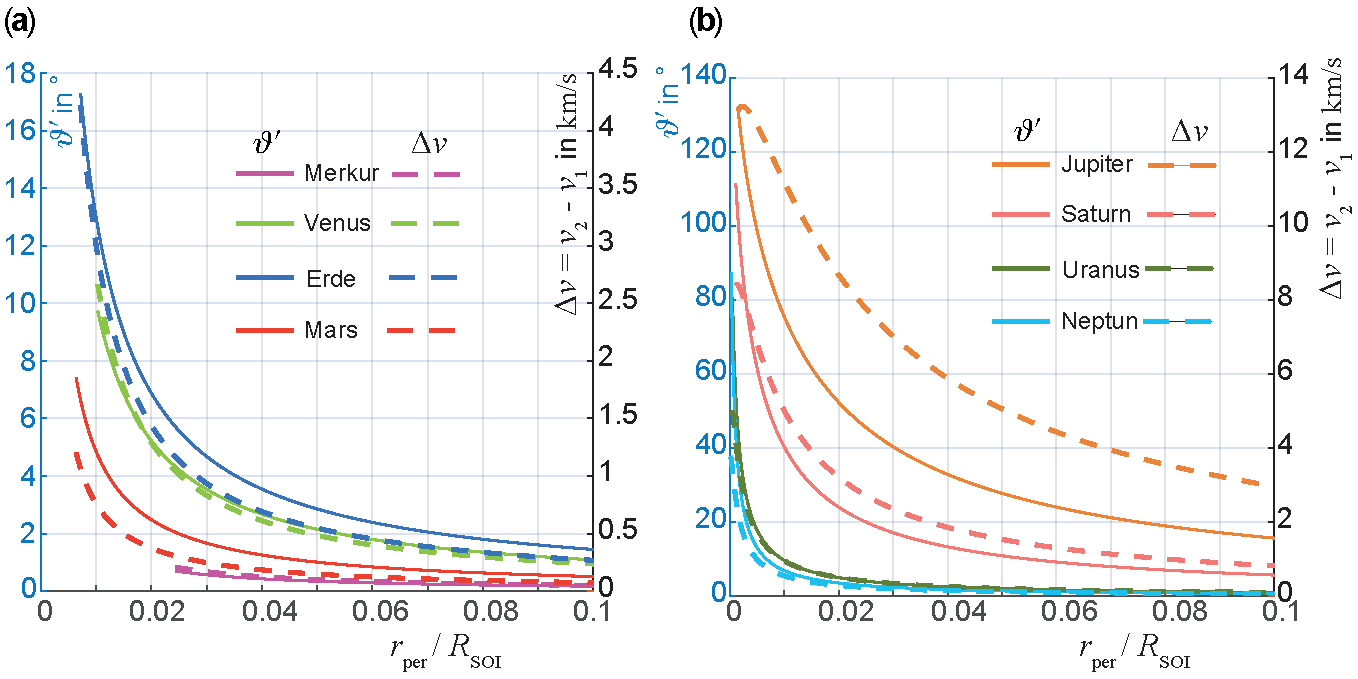
\includegraphics[width=\textwidth]{SwingByPlaneten.pdf} 
	\caption[Swing-By-Man�ver Ergebnisse bei den Planeten unseres Sonnensystems.]{Swing-By-Man�ver Ergebnisse bei den Planeten unseres Sonnensystems  als Funktion des periplanetaren Abstands $r_\text{per}$ normiert auf den Radius der SOI $R_\text{SOI}$, \fa innere Planeten \fb �u�ere Planeten. F�r die inneren Planeten wurde ein Eingangswinkel $\gamma_1 = 20\degree$ gew�hlt, f�r die �u�eren Planeten $\gamma_1 = 60\degree$. In beiden F�llen wurde $v_1= \SI{12.7}{\km\per\second}$ gesetzt. Alle anderen Werte siehe Tabelle \ref{tab:adyn_results_swingby}.}
	\label{abb:adyn_swingby02a}
\end{figure}

Da beim Swing-By $m_\text{P}$ (\bzw $\mu_\text{P}$) und $v_\text{P}$ festliegen, bleiben als freie Parameter nur $r_\text{per}$ und $\beta_1'$ (\bzw $\gamma_1$) �brig. Den Parameter $r_\text{per}$ k�nnen wir aus der Hyperbelgleichung berechnen:
\begin{align}
    r_\text{per} = a\lk 1- e\rk = \frac{\mu_\text{P}}{v_\infty{}^2}\,\lk e-1\rk \,, \label{eq:adyn_swingby16}
\end{align}
mit $e = 1/\cos\varphi'$. Der maximale Energie�bertrag erfolgt, wenn $\beta_2{}'=0$ ist, \dh die Vektoren $\vec{v}_2{}'$ und $\vec{v}_\text{P}$ parallel sind. Dann ist $\varphi'=90\degree-\beta_1{}'/2$ und somit $\cos\varphi'= \sin(\beta_1{}'/2)$ und wir erhalten f�r den optimalen Minimalabstand zum Perizentrum, bei dem der Energie�bertrag maximal wird: 
\begin{align}
    r_\text{P, opt} = \frac{\mu_\text{P}}{v_\infty{}^2}\,\lek \frac{1}{\sin\lk\beta_1{}'/2\rk}-1\rek > R_\text{P} \,.\label{eq:adyn_swingby17}
\end{align}
Dieser Abstand muss logischerweise immer gr��er als der physische Planetenradius $R_\text{P}$ sein, kann also durch geschickte Wahl von $v_1$ und $\gamma_1$ (und damit $v_1{}'$ und $\beta_1{}'$) entsprechend gew�hlt werden.\\
In \figref{adyn_swingby02a} haben wir $\Delta v = v_2-v_1$  und $\vartheta' = \Delta \gamma = \gamma_2 -\gamma_1$ als Funktion des Parameters $r_\text{per}$ �ber $\gamma_1$ dargestellt. \figref{adyn_swingby02} zeigt die gleichen Gr��en f�r die verschiedenen Planeten unseres Sonnensystems f�r einen vorgegebenen Wert von $v_1$ und $\gamma_1$ als Funktion des auf den Radius der SOI $R_\text{SOI}$ normierten Perizentrumsabstands $r_\text{per}$. Dabei haben wir f�r die Planeten jeweils den Bereich von $r_\text{per} = R_\text{P} + 500\,\mathrm{km}$ (inklusive Sicherheitsabstand von der Oberfl�che!) bis zu $0.1\,R_\text{SOI}$, \dh 10\% des Radius der jeweiligen SOI ausgew�hlt. Man erkennt, dass es signifikante Energie�bertr�ge vor allem bei den massereichen Planeten Jupiter und Saturn gibt, aber auch durch m�gliche "`nahe"' Vorbeifl�ge bei Venus und Erde (Tabelle \ref{tab:adyn_results_swingby}).\\ 

\begin{table}%tab 
\caption{Swing-By-Man�ver Daten f�r die Planeten unseres Sonnensystems.}
\smallskip
\begin{tabular}{L{0.8cm}R{1.35cm}R{1.65cm}R{1.25cm}R{1.25cm}R{1.25cm}R{1.25cm}R{1.65cm}R{1.25cm}}
\svhline\noalign{\smallskip}
Planet				& $v_\text{P}$                     & $m_\text{P}$     & $a_\text{P}$     & $R_\text{SOI}$  & $R_\text{P}$ & $v_{1,\text{max}{}'}$        & $\Delta H_\text{max}$& $\vartheta_\text{max}{}'$\\ 
\noalign{\smallskip}\noalign{\smallskip}              
& $\SI{}{\kilo\metre\per\second}$  & $\SI{}{\kg}$     & $10^6\,\SI{}{\km}$ & $10^6\,\SI{}{\km}$& $\SI{}{\km}$ & $\SI{}{\km\per\second}$   & $\SI{}{\joule\per\kg}$  &$\degree$\\ 
\noalign{\smallskip}\noalign{\smallskip}              
\noalign{\smallskip}\svhline\noalign{\smallskip} 
Merkur				& 47.9          & $\SI{3.28e23}{}$ &  57.9        & 0.11          & 2439         & 2.99                 & $\SI{1.43e8}{}$ & 6.1\\
Venus 				& 35.0          & $\SI{4.87e24}{}$ & 108.2        & 0.62          & 6051         & 7.33                 & $\SI{2.57e8}{}$ & 28.9\\
Erde 	  			& 29.8          & $\SI{5.97e24}{}$ & 149.6        & 0.93          & 6378         & 7.90                 & $\SI{2.35e8}{}$ & 32.4\\
Mars   				& 24.1          & $\SI{6.42e23}{}$ & 228.0        & 0.58          & 3394         & 3.55                 & $\SI{0.86e8}{}$ & 8.3\\
Jupiter 			& 13.1          & $\SI{1.90e27}{}$ & 778.4        &48.20          &71400         &42.1                  & $\SI{5.50e8}{}$ & 132.9\\
Saturn  			&  9.6          & $\SI{5.69e26}{}$ & 1425.5       &54.8           &60000         &25.2                  & $\SI{2.43e8}{}$ & 105.6\\
Uranus 				&  6.8          & $\SI{8.68e25}{}$ & 2870.4       &51.7           &26650         &15.0                  & $\SI{1.02e8}{}$ & 71.4\\
Neptun 				&  5.4          & $\SI{1.03e26}{}$ & 4501.1       &86.7           &24780         &16.7                  & $\SI{0.91e8}{}$ & 78.2\\
\svhline\noalign{\smallskip}
\end{tabular} \\
\label{tab:adyn_results_swingby}
\end{table}%tab 

Wie erw�hnt wird das Gravity-Assist-Man�ver bei vielen interplanetaren Raumfl�gen angewendet. 
Dabei benutzt man f�r die Missionsplanung die sogenannte \textit{Patched-Conic-} N�herung\index{Patched-Conic-N�herung}. Bei dieser N�herung wird die Trajektorie der Raumsonde in verschiedene Abschnitte unterteilt, indem jedem Himmelsk�rper (Sonne, Mond, Planeten) seine eigene Einflusssph�re (SOI) zugeordnet wird. Wenn die Sonde innerhalb der SOI des jeweiligen Himmelsk�rpers ist, wird nur dessen Gravitationskraft ber�cksichtigt, au�erhalb bei interplanetaren Fl�gen dann \ia nur die der Sonne. Dieses Vorgehen reduziert das $N$-K�rper-Problem auf ein Zweik�rperproblem, f�r das wir die bekannten parabolischen, elliptischen \bzw hyperbolischen L�sungen kennen.\footnote{Man �berlege sich, unter welchen Bedingungen die Methode nicht zum Erfolg f�hrt. Hinweis: Lagrange-Punkte (Band I, Kapitel 1.2.3.6.} 
Als Beispiel sei ein Erde-Mars-Transfer betrachtet (\vgl \probref{adyn_manoevers5}). Hier folgt die Raumsonde zun�chst einer hyperbolischen Bahn, um den Anziehungsbereich der Erde zu verlassen, dann folgt sie \ia einer Kepler-Ellipse um die Sonne, um schlie�lich in die Einflusssph�re des Mars zu treten. Durch das Zusammenf�gen der einzelnen Kegelschnittbahnen erh�lt man in guter N�herung die tats�chliche Bahn, daher auch der Name der N�herung (Englisch \textit{ to patch }- zusammenf�gen).\\
Selbstverst�ndlich kann man bei den Missionsplanungen zu �u�eren Planeten mit dieser Methode Gravity-Assist-Man�ver einbauen. In der Literatur (\ua \cite{Minovitch2010, Walter2018, Messerschmid2017}) finden sich dazu zahlreiche Beispiele. Wir wollen die zum Zeitpunkt des Verfassens dieses Buches im Jahre 2023 gestartete ESA-Mission JUICE (\textit{\underline{Ju}piter \underline{I}cy \underline{M}oon \underline{E}xploration}) etwas genauer betrachten und beziehen uns dabei auf \cite{Althaus2023}.

\begin{figure}[H]
	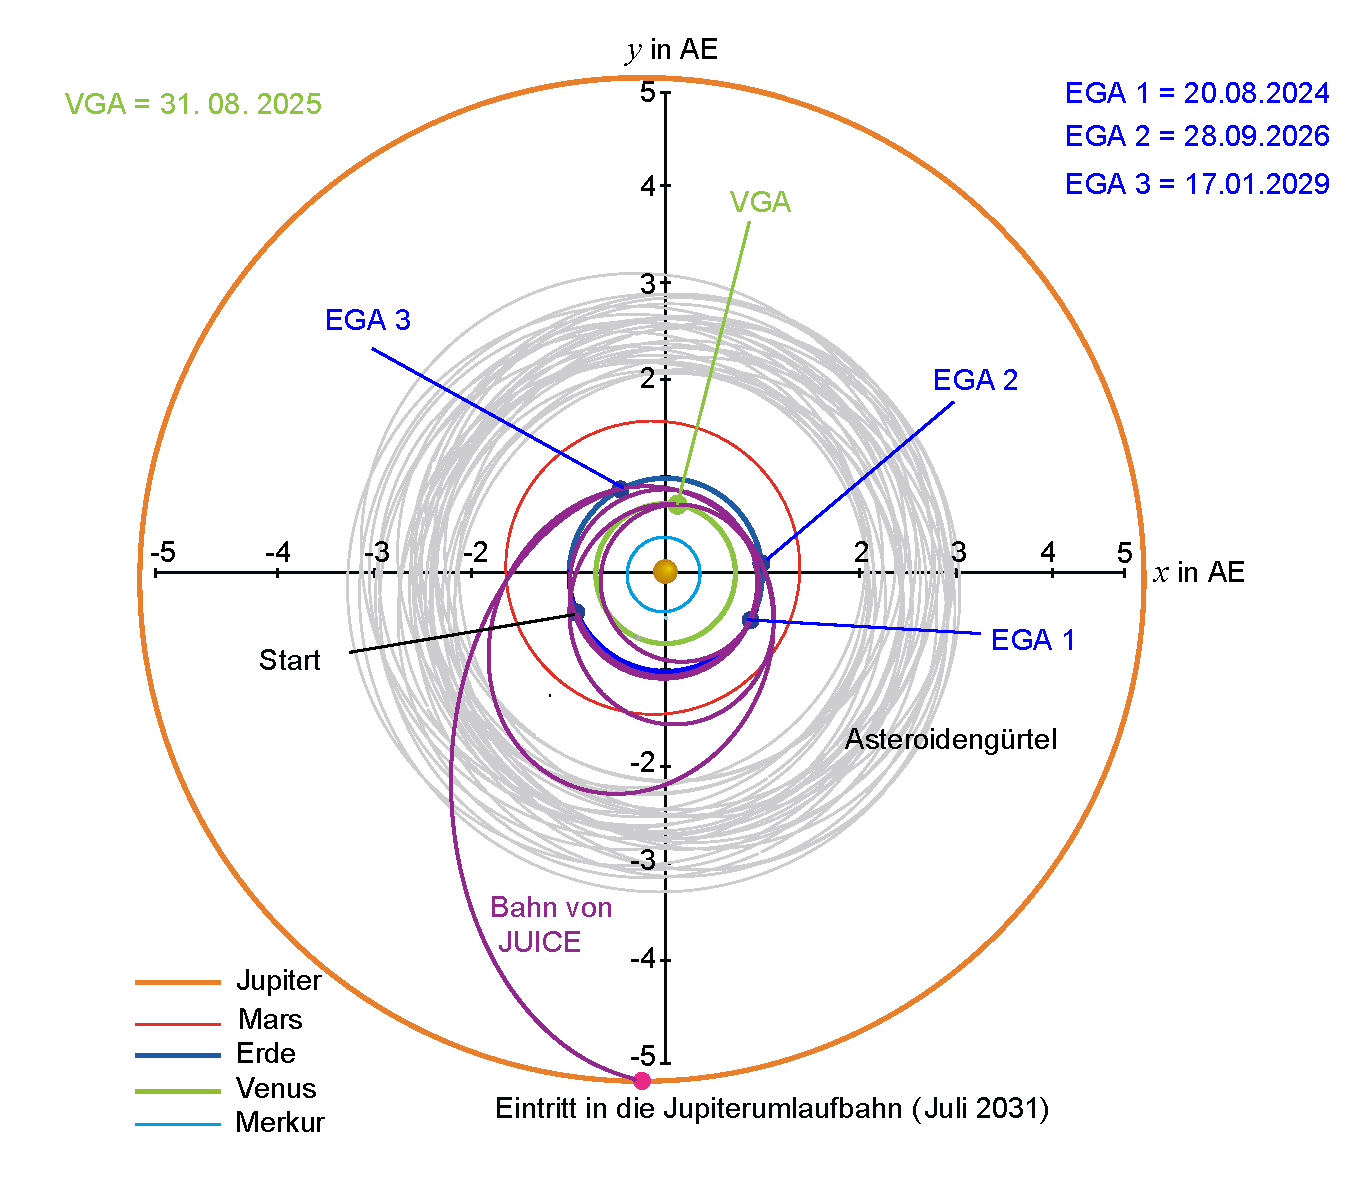
\includegraphics[width=\textwidth]{MissionJUICE.pdf} 
	\caption[Interplanetare Flugplanung der ESA-Mission JUICE.]{Interplanetare Flugplanung der ESA-Mission JUICE. Nach \cite{Althaus2023}.}
	\label{abb:adyn_PSP01}
\end{figure}

Die beeindruckende Reise dieser Raumsonde zu den Jupiter-Monden mit dem geplanten Eintritt in die Jupiterumlaufbahn im Jahr 2031 erfordert insgesamt vier Planeten-Vorbeifl�ge (\gls{GA}), dreimal an der Erde (EGA, \gls{EGA}) und einmal an der Venus (VGA, \gls{VGA}). Das erste EGA am 20.08.2024 f�hrte zu einer Abbremsung und damit zu einer engen Bahn um die Venus, von wo aus sie dann wieder beschleunigt wird und beim geplanten VGA am 31.08.2025 ein $\Delta v = \SI{3.8}{\km\per\second}$ erhalten wird ($r_\text{min} = \SI{5100}{\km} + R_\text{v}$). Der erneute Erdvorbeiflug am 28.09.2026 wird die Geschwindigkeit nochmals um $\Delta v = \SI{3.5}{\km\per\second}$ ($r_\text{min}= \SI{8600}{\km} + R_\text{E}$) erh�hen.\footnote{In \probref{adyn_PSP01} vergleichen wir die in den Vorbeifl�gen an Erde und Venus erreichten Geschwindigkeitszuw�chse von JUICE mit den maximal erreichbaren $\Delta v$ bei Venus und Erde (Tabelle \ref{tab:adyn_results_swingby}) und den Rechnungen in \probref{adyn_swingby01}.} 
%Die Sonde hat nun ausreichend Energie, um auf einer weiten elliptischen Bahn um die Sonne den Rand des Asteroideng�rtels zu erreichen, bevor sie 
Beim letzten EGA am 17.01.2029 wird sie noch ein $\Delta v = \SI{3.5}{\km\per\second}$ ($r_\text{min} = \SI{4600}{\,\km} + R_\text{E}$) bekommen, das sie endlich auf eine elliptische Bahn zum Jupiter (\figref{adyn_PSP01}) bringt. 

\subsection{Interplanetarer Raumflug zur Sonne}\label{kap:adyn_interplanetary_flights}

Wir hatten bereits in \figref{adyn_swingby00} gesehen, dass der Geschwindigkeitsgewinn $\Delta v$ bei einem Swing-By-Man�ver sowohl positiv als auch negativ sein kann. Wir wollen nun den Fall betrachten, bei dem man ein negatives $\Delta v$ braucht, um \zb eine Sonde so abzubremsen, dass sie auf eine sehr enge Umlaufbahn um die Sonne gelangen kann. Ein solche Mission ist die NASA-\textit{Parker}\footnote{Eugene Newman Parker (1927--2022) war ein US-amerikanischer Astrophysiker, der vor allem den Sonnenwind, die Magnetfelder von Erde und Sonne und deren komplexe Wechselwirkungen untersuchte. Er pr�gte auch als erster den Begriff \gls{Sonnenwind}\index{Sonnenwind} (\textit{solar wind}).}\indexp{Parker, Eugene Newman} \textit{Solar Probe}-Mission (PSP), die am 12.08.2018 gestartet wurde und zum Ziel hat, einen Minimalabstand zur Sonne von $r_\text{S}= \SI{0.05}{AE}$ zu erreichen. Was ist dabei eigentlich die Schwierigkeit? Man k�nnte meinen, dass eine Sonde einmal von der Erde in Richtung Sonne auf den Weg gebracht, von dieser so angezogen wird, dass die Sonde fr�her oder sp�ter in den Einfangbereich der Sonne gelangt und dann dort quasi von dieser in sich hineingezogen wird. Dem widersprechen aber die Gesetze der Himmelsmechanik, insbesondere die Drehimpuls- und Energieerhaltung. 
Um wirklich eine Sonde direkt zur Sonne zu senden, m�sste man ja durch Raketenenergie den Drehimpuls auf ann�hernd Null bringen, was bedeutet, dass man beim Start auf einer Erdbahn ein Antriebsbudget von etwa $\Delta v = - v_\text{E} = - \sqrt{2\mu_\text{S}/1\au} = -\SI{29.8}{\kilo\metre\per\second}$ haben muss. Die Sonne ist damit der am "`schwierigsten"' zu erreichende Platz in unserem Sonnensystem. 
Wir wollen den Antriebsbedarf etwas genauer absch�tzen, den man br�uchte, wenn man eine sonnennahe Bahn mit Minimalabstand $r_\text{min}$ durch einen Flug direkt aus einer Erdumlaufbahn erreichen wollte. Wir nehmen der Einfachheit halber einen Hohmann-Transfer mit $a_\text{H} = \frac{1}{2}\,\lk 1 \au + r_\text{min}\rk$ und $v_1 = v_\text{E} = \SI{29.8}{\km\per\second}$ an. Dann ergibt sich mit dem vis-viva-Satz\index{vis-viva-Satz} ein Geschwindigkeitsbedarf von 
\begin{align}
    \Delta v &\approx v_\text{P} -v_\text{E} = \sqrt{\mu_\text{S}\,\lk \frac{2}{0.05\au} - \frac{1}{a_\text{H}}\rk} - v_\text{E}
		= \sqrt{\frac{\mu_\text{S}}{1\au}}\,\sqrt{\lk \frac{2}{0.05\au} - \frac{2}{1.05\au}\rk} - v_\text{E} \nonumber  \\
		&= v_\text{E}\,\lk \sqrt{2\,\lk 1-\frac{1}{1.05}\rk} -1\rk \approx -\SI{20.6}{\km\per\second}\,.\label{eq:adyn_abschaetzung}
\end{align}
Mit der Ariane 5 schafft man es, eine Sonde mit einer Masse von $\SI{6}{\tonne}$ mit einer Geschwindigkeit von \ca $\SI{12.7}{\km\per\second}$ auf die Reise zu schicken (gemessen im \KOS\ der Erde, also vergleichbar mit dem $\Delta v$ aus \eqref{eq:adyn_abschaetzung}). Wir sehen also, dass es beim Stand der heutigen Raketentechnik nicht m�glich w�re, eine Sonde direkt zur Sonne zu schicken, die einen Minimalabstand von $0.05\,\au$ erreicht.\footnote{Zum Vergleich: Die gro�e Halbachse der Merkurbahn betr�gt $\SI{0.3871}{AE}$, also das etwa 8-fache.}
Wir wollen nun die Planung der PSP-Mission genauer betrachten. Die PSP soll die �u�ersten Atmosph�renschichten der Sonne und deren \gls{Korona}\index{Korona!der Sonne} erforschen und am 24.12.2024 den sonnenn�chsten Punkt der gesamten Mission mit $a_\text{P}= \SI{0.046}{}\,\au = \SI{6.8e6}{\kilo\metre}$ (Perihel ihres solaren Orbits) erreichen. Das ist nur das 18-fache des Erde-Mond-Abstands. N�her an die Sonne ist bisher noch keine Sonde gekommen. Die PSP nutzt bei ihrer Ann�herung an die Sonne verschiedene Gravity-Assists aus, um ihre Bahnenergie zu reduzieren. Wir wollen uns das Prinzip etwas genauer anschauen und treffen als Vereinfachung die Annahme, dass alle Bewegungen in der Ekliptik erfolgen.\\
Wenn eine Sonde von der Erde mit einem $\Delta \vec{v}_\text{R}$ gestartet wird, dann folgt diese einem elliptischen Orbit, der die SOI der Erde (oder auch der Venus) zu einem bestimmten Zeitpunkt wieder "`kreuzen"' wird, siehe \figref{adyn_swingby04}. An diesem Kreuzungspunkt $\mathrm{P}_1$ soll nun ein Gravity-Assist-Man�ver stattfinden.\footnote{Es gibt ja einen weiteren Kreuzungspunkt $\mathrm{P}_1'$, an dem ein Man�ver stattfinden kann. Zur Unterscheidung bezeichnen wir das Man�ver bei $\mathrm{P}_1$ als Planeten-ann�hernd und bei $\mathrm{P}_1'$ als Planeten-entfernend. Im weiteren wollen wir uns auf das erstere beschr�nken.} 

\begin{figure}[H]
	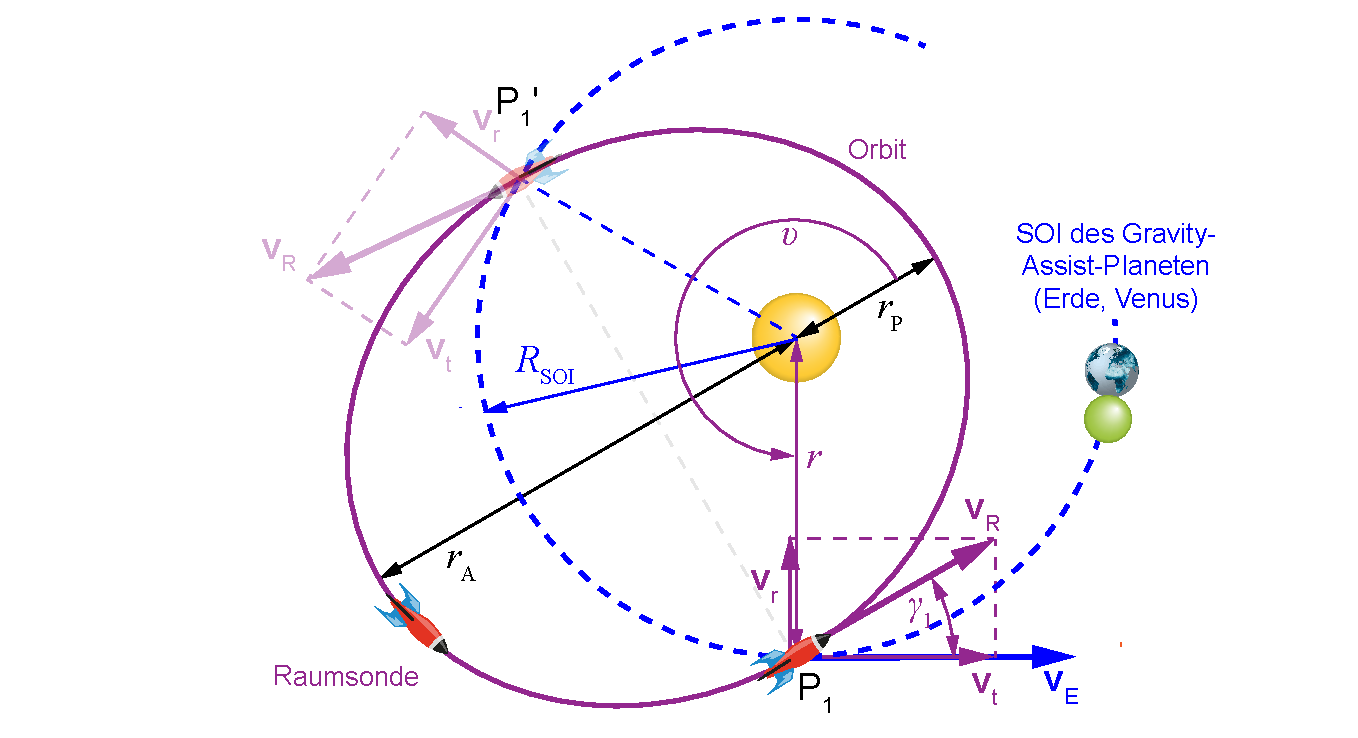
\includegraphics[width=\textwidth]{OrbitCrossing.pdf} 
	\caption[Gravity-Assist-Man�ver - Orbital Crossing.]{Gravity-Assist-Man�ver - Eine elliptische Bahn einer Sonde (lila) kreuzt die Einflusssph�re eines Planeten, hier der Erde (blau gezeichnet). Die Momentangeschwindigkeit der Sonde und auch die radiale und tangentiale Komponente sind als lila Vektoren dargestellt.}
	\label{abb:adyn_swingby04}
\end{figure}

Zur Berechnung brauchen wir den Vektor der Geschwindigkeit der Sonde an diesem Punkt~$\mathrm{P}_1$ im heliozentrischen Koordinatensystem. Dieser Vektor ist eine Funktion der Parameter der momentanen Bahn der Sonde und wir k�nnen ihn in einen radialen und einen zur SOI tangentialen Anteil zerlegen:
\begin{align}
	  \vec{v}_1 =\vec{v}_\text{R} = v_\text{r}\,\vec{e}_\text{r} + v_\text{t}\,\vec{e}_\text{t}\,.\label{eq:adyn_PSP01}
\end{align}
Dies hat den Vorteil, dass am Punkt $\mathrm{P}_1$ die Tangentialkomponente parallel zum Vektor der Planetengeschwindigkeit ist. Zur Vereinfachung nehmen wir an, dass die Sonde am Punkt~$\mathrm{P}_1$ zwar in die Einflusssph�re des Gravity-Assist-Planeten gelangt, aber immer noch einen Abstand zur Sonne von etwa dem Bahnradius (1\,AE f�r die Erde \bzw 0.723\,AE f�r die Venus) haben soll.\\
Wir nutzen die Erhaltungss�tze und schreiben mit $\mu_\text{S} = G\,m_\text{S}$ und den Parametern $a,\,e$ der Bahnellipse: 
\begin{align}
\begin{split}
	  \text{Drehimpulserhaltung, vgl. \eqref{eq:hm_drehimpuls_von_ae}} ~~~~L^2 &= r^2\, v_\text{t}{}^2 = \mu_\text{S}\,a\,\lk 1-e^2 \rk \,, \\
		\text{Energieerhaltung, vgl. \eqref{eq:hm_bewgl1}}~~~~H &= \frac{1}{2} \left| \vec{v}_\text{R} \right|^2 - \frac{\mu_\text{S}}{r} = - \frac{\mu_\text{S}}{2\,a}\,.
\end{split}  \label{eq:adyn_PSP02}
\end{align}
Aus der Ellipsengleichung \eqref{eq:hm_bahnglg}
\begin{align}
r(\upsilon) = \frac{a(1-e^2)}{1+e\,\cos\lk\upsilon-\upsilon_\text{P}\rk} \label{eq:adyn_PSP03}
\end{align}
mit $a = \lk r_\text{P} + r_\text{A} \rk /2$ und Perihel- \bzw Aphelabstand\index{Aphel}\index{Perihel} von $r_\text{P} = a\,(1-e)$ \bzw $r_\text{A} = a\,(1+e)$ erhalten wir f�r das Verh�ltnis von gro�er Halbachse $a$ der Sondenbahn und dem Radius der SOI, den wir vereinfacht schreiben als $R_0 = R_\text{SOI} = 1\,\au$ (\bzw $R_0 = 0.723\,\au$ f�r die Venus):
\begin{align}
	\frac{a}{R_0} = \frac{1}{2-\left|\vec{v}_\text{R} \right|^2 / v_0{}^2}\,, \label{eq:adyn_PSP04}
\end{align}
worin $v_0 = \sqrt{\mu_\text{S}/ R_0}$ ist. Aus \eqref{eq:adyn_PSP04} erhalten wir $\left|\vec{v}_\text{R} \right| = v_\text{R}$. Ferner folgt aus der Drehimpulserhaltung aus \eqref{eq:adyn_PSP02} f�r die Tangential- und Radialkomponente $v_\text{t}$ \bzw $v_\text{r}$
\begin{subequations}
\begin{align}
	v_\text{t} &= v_0\, \sqrt{\frac{a}{R_0}\,\lk 1-e^2 \rk} \,, \label{eq:adyn_PSP05a} \\
	v_\text{r} &= \sqrt{\left|\vec{v}_\text{R} \right|^2 - v_\text{t}{}^2} \,. \label{eq:adyn_PSP05b}
\end{align} 
\end{subequations} \label{eq:adyn_PSP05}

Damit k�nnen wir nun die f�r die Berechnung des Streuwinkels aus \eqref{eq:adyn_Streuung13b} noch fehlende Gr��e $v_\infty{}$ �ber \eqref{eq:adyn_swingby01a} berechnen: 
\begin{align}
	v_\infty{}  = \sqrt{v_\text{r}{}^2 - \lk v_\text{t} - v_0 \rk^2} \,. \label{eq:adyn_PSP06}
\end{align} 
Wir setzen nun f�r die initiale Bahn (Index a) der PSP die Werte $r_\text{P} = 0.207\,\au,\,~r_\text{A} = 1.013\,\au$ ein und erhalten: 
\begin{align*}
  v_\text{t} &= \SI{24.1}{\km\per\second}\,,~~~v_\text{r} = \SI{20.4}{\km\per\second}\,,~~~v_0 = \SI{35.02}{\km\per\second}\,~~
	\rightarrow v_\infty{}  = \SI{23.4}{\km\per\second}\,.
\end{align*}
F�r die Venus erhalten wir mit $\mu_\text{V} = G\,m_\text{V}$ f�r $\tilde{v}_\text{F}$ aus \eqref{eq:adyn_swingby09c}:
\begin{align}
    \tilde{v}_\text{F} &= \sqrt{\frac{2 \mu_\text{V}}{R_\text{V} + \SI{500}{km}}} = \SI{9.95}{\km\per\second}\,, \label{eq:adyn_PSP07} 
\end{align}
woraus sich bei einem Sicherheitsabstand des Swing-By-Man�vers von 500 km von der Venusoberfl�che ein maximaler Streuwinkel von $\vartheta'_\text{a} = 9.73\degree$ ergibt. 

\begin{table} [ht] %tab 
\caption{Die einzelnen Orbits der NASA Mission Parker Solar Probe I um die Sonne.}
\smallskip
\begin{tabular}{C{0.8cm}R{1.5cm}R{1.5cm}R{1.5cm}C{1.5cm}R{1.75cm}R{1.75cm}}
\svhline\noalign{\smallskip}
Orbit &  $r_\text{P} \, (\au)$  & $r_\text{A} \, (\au)$ & $\beta_1'\, (\degree)$ &   $ e $    &  $ T_\text{Bahn}$ \, (Tage) & $v_\text{P}\,(\SI{}{\km\per\second})$\\
\noalign{\smallskip}\svhline\noalign{\smallskip} 
\noalign{\smallskip}\noalign{\smallskip}              
  a    &   0.207     &   1.013    &   61.94     &  0.661   &    174.0     &   84.35 \\
  b    &   0.166     &   0.938    &   55.58     &  0.699   &    149.8     &   95.29 \\
  c    &   0.130     &   0.874    &   48.43     &  0.741   &    129.9     &  108.99 \\
  d    &   0.095     &   0.817    &   39.42     &  0.792   &    112.5     &  129.34 \\
  e    &   0.074     &   0.783    &   31.99     &  0.827   &    102.5     &  147.99 \\
  f    &   0.062     &   0.761    &   25.77     &  0.849   &     96.4     &  162.65 \\
  g    &   0.053     &   0.745    &   19.74     &  0.867   &     92.1     &  176.77 \\
  h    &   0.046     &   0.731    &   11.99     &  0.882   &     88.5     &  190.47 \\
\svhline\noalign{\smallskip}
\end{tabular} \\
\label{tab:adyn_PSP01}
\end{table}%tab 

Dieser Streuwinkel ist deutlich kleiner als der notwendige Streuwinkel von $\Delta \vartheta' = \beta_{1,\text{a}}{}' - \beta_{1,\text{h}}{}' \approx 50\degree$, den man br�uchte, wenn man durch ein Swing-By-Man�ver direkt von der Anfangsbahn mit $r_\text{P,a} = 0.207\,\au,\,~r_\text{A,a} = 1.013\,\au$ auf die vorgesehene finale Bahn mit $r_\text{P,h} = 0.046\,\au,\,~r_\text{A,h} = 0.731\,\au$ gelangen m�chte. Dazu br�uchte man (siehe Tabellen \ref{tab:adyn_PSP01} und \ref{tab:adyn_PSP02}) also mindestens 6 Gravity-Assist-Man�ver an der Venus. Die tats�chliche Mission nutzte insgesamt 7 solcher Swing-By-Man�ver, deren Abfolge mit den einzelnen Streuwinkeln, den kumulierten Streuwinkeln und den realisierten Perizentrumsabst�nden $R_\text{V,real}$ der jeweiligen Swing-By-Man�ver in Tab. \ref{tab:adyn_PSP02} und \figref{adyn_swingby05} dargestellt sind. Eine vertiefte Betrachtung zu der Missionsplanung der PSP, in der auch ein elegantes graphisches Tool zur Bestimmung der Bahnen, die sogenannte \textit{Velocity-Space-Map},  vorgestellt wird, findet sich in \cite{Longcope2020}.

\begin{table} [ht] %tab 
\caption{Die einzelnen Swing-By-Man�ver der NASA Mission Parker Solar Probe I an der Venus.}
\smallskip
\begin{tabular} {C{1.75cm}R{1.75cm}R{1.75cm}R{1.75cm}}
\svhline\noalign{\smallskip}
GA-Man�ver &  $\vartheta' \,(\degree)$  &  $\sum\vartheta'\, (\degree)$  & $R_\text{V,real}/R_\text{V}$\\
\noalign{\smallskip}\svhline\noalign{\smallskip} 
\noalign{\smallskip}\noalign{\smallskip}              
   1\,:\;(a $\,\rightarrow\,$ b)  &    6.501    &      6.501        &   1.67  \\
   2\,:\;(b $\,\rightarrow\,$ c)  &    7.157    &     13.658        &   1.49  \\
   3\,:\;(c $\,\rightarrow\,$ d)  &    9.113    &     22.771        &   1.15  \\
   4\,:\;(d $\,\rightarrow\,$ e)  &    7.389    &     30.160        &   1.43  \\
   5\,:\;(e $\,\rightarrow\,$ f)  &    6.229    &     36.389        &   1.70  \\
   6\,:\;(f $\,\rightarrow\,$ g)  &    5.948    &     42.337        &   1.79  \\
   7\,:\;(g $\,\rightarrow\,$ h)  &    7.628    &     49.965        &   1.37  \\
\svhline\noalign{\smallskip}
\end{tabular} \\
\label{tab:adyn_PSP02}
\end{table}%tab 

\begin{figure}[H]
	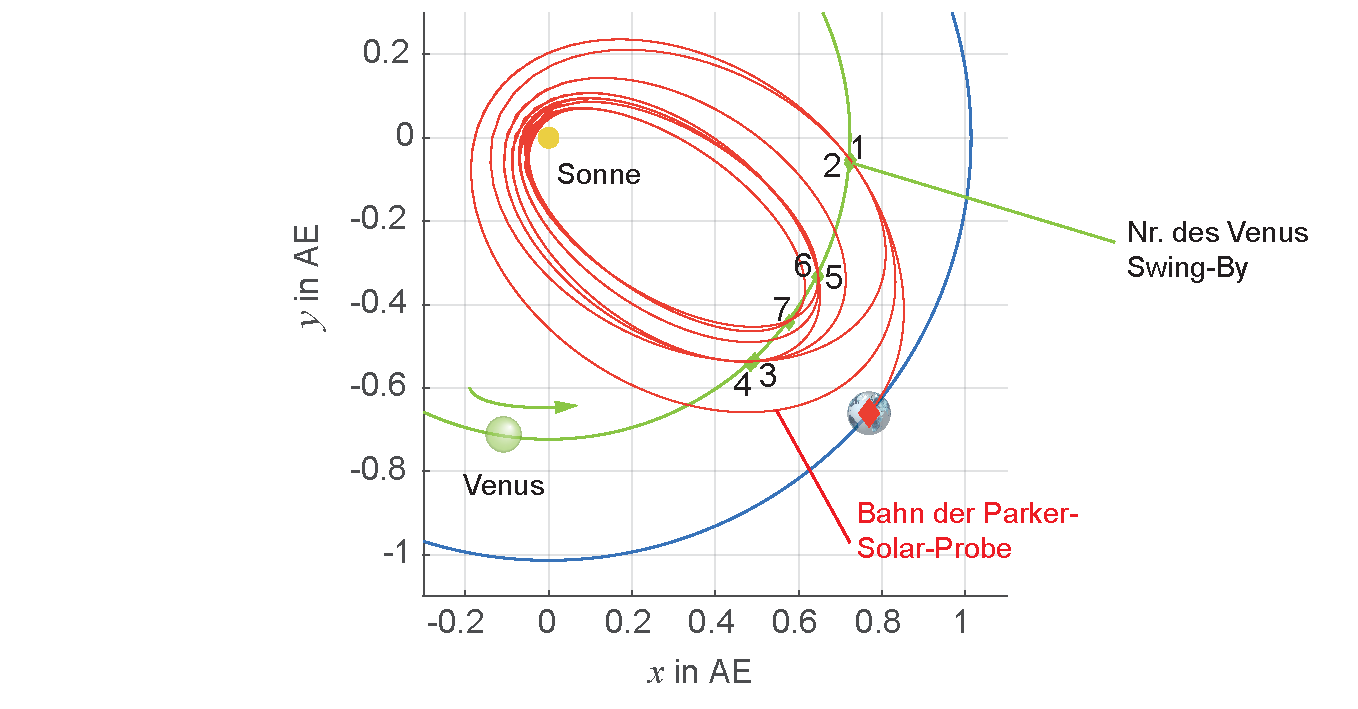
\includegraphics[width=\textwidth]{BahnParkerSolarProbe.pdf} 
	\caption[Die NASA Mission Parker Solar Probe.]{Die NASA Mission Parker Solar Probe. Dargestellt ist die Bahn der PSP vom Start bis zum 30.1.2024. Die Rauten geben die Punkte der Venus-Swing-By-Man�ver an. Die Daten der PSP-Bahn stammen vom JPL \cite{JPL2020}, k�nnen aber nat�rlich genau so wie die Planetenbahnen von Venus und Erde mit den Methoden aus dem \kap{hm_bahnen_hk_ss} aus der Himmelsmechanik berechnet werden. Sehr gut zu erkennen ist, wie mit jedem Swing-By-Man�ver die Sonde sukzessive auf eine engere Bahn um die Sonne gelangt. Siehe auch \probref{adyn_PSP01} und \mscr~ \mladynref{ParkerSolarProbe.m}.}
	\label{abb:adyn_swingby05}
\end{figure}















\clearpage
\section{Rendezvous im Weltall}\label{kap:adyn_planetflights}

\subsection{Dynamik und Kinematik eines Kopplungsman�vers }\label{kap:adyn_rendezvous}

Wir wollen uns jetzt das Rendezvous\index{Rendezvouz} (\bzw das Andocken) zwischen zwei Raumschiffen, \zb einem Raumtransporter (\emph{"`Verfolger"'}, englisch \textit{Interceptor, Chaser}, Index J) und einer Raumstation (\zb der ISS) in einer Umlaufbahn  (dem \textit{"`Ziel"'}, englisch \textit{Target}, Index T) anschauen und folgen hier der Darstellung in \cite{Carroll2019}.
Die mathematische Beschreibung des Rendezvous von zwei Raumschiffen im Weltall ist relativ komplex, was unter anderem auch daran liegt, dass die Bewegung der beiden Raumschiffe zueinander, wenn man sie aus einem mit einem der Raumschiffe verbundenen Koordinatensystem beschreibt, dann in einem rotierenden nicht inertialen Koordinatensystem beschrieben werden muss\footnote{Wir werden dabei gewisse �hnlichkeiten mit dem Fahren auf einer rotierenden Scheibe (\vgl �bung 1.21 in Band I) feststellen.}.\\
Wir bezeichnen das Inertialsystem mit Ursprung im Erdmittelpunkt mit $\vec{\Sigma}$ und das mitbewegte System, welches seinen Ursprung im Ziel (in der ISS) mit $\vec{\Sigma}'$. Die $z$-Achsen beider Systeme sind parallel und zeigen senkrecht aus der Bahnebene heraus (\figref{adyn_rendezvousKOS01}). Die Koordinaten des Verfolgers (des Raumtransporters) haben daher einen Strich, wenn sie vom Ziel aus gemessen werden, sie sind ohne Strich, wenn sie von der Erde aus gemessen werden.\\
F�r die Kopplung\footnote{Wir benutzen den Begriff Kopplung und Rendezvous hier synonym, obwohl im strengen Sinne der Astrodynamik mit Rendezvous die Begegnung zweier Raumschiffe durch entsprechende Bahnman�ver und mit Kopplung der gesamte mechanische Vorgang der Verbindung zweier Raumschiffe bezeichnet wird.} zweier Objekte im Weltall muss zum Zeitpunkt $t_\text{K}$ der Kopplung im Koordinatensystem der Erde $\vec{\Sigma}$ \bzw im System des Ziels $\vec{\Sigma}'$ gelten:
\begin{align}
\begin{split}
    \vec{\Sigma}: ~~~~ \vec{r}_\text{T}\lk t_\text{K}\rk &= \vec{r}_\text{J}\lk t_\text{K}\rk ~~ \text{und} ~~~  \dot{\vec{r}}_\text{T}\lk t_\text{K}\rk = \dot{\vec{r}}_\text{J}\lk t_\text{K}\rk \,, \\
    \vec{\Sigma}': ~~~\,~  \vec{r}'\lk t_\text{K}\rk &= 0 ~~ \text{und} ~~~ \dot{\vec{r}}'\lk t_\text{K}\rk = 0 \,. 
\end{split} \label{eq:adynrendez01}
\end{align}
Die Bedingungen f�r die Geschwindigkeit sichern eine \anf{weiche} Kopplung.\\
Wir bezeichnen die Position des Ziels (\figref{adyn_rendezvousKOS01}) im Inertialsystem mit:
\begin{align}
    \vec{R} = X\,\vec{e}_x + Y\,\vec{e}_y + 0\,\vec{e}_z = R_0\,\vec{e}_{y'} ~~~~ \text{mit} ~~~~ R_0 = \sqrt{X^2+Y^2}\,,\label{eq:adyn_rendez01}
\end{align}
entsprechend die des Verfolgers mit
\begin{align}
    \vec{r} = x\,\vec{e}_x + y\,\vec{e}_y + z\,\vec{e}_z\label{eq:adyn_rendez02}\,,
\end{align}
\bzw im mitbewegten \KOS\ mit
\begin{align}
    \vec{r}' = x'\,\vec{e}_{x'} + y'\,\vec{e}_{y'} + z'\,\vec{e}_{z'}\label{eq:adyn_rendez03}\,.
\end{align}
%Um ein Rendezvous im Weltall durchzuf�hren, ist die Beschreibung der Bewegung als Relativbewegung von Ziel und Verfolger sinnvoll, und zwar am einfachsten vom Ziel aus betrachtet. 
Es gelten dann folgende Bewegungsgleichungen f�r die Koordinaten des Verfolgers im nichtinertialen \KOS\ des Ziels:
\begin{align}
\begin{split}
    \vec{r}' &= \vec{r} - \vec{R}\,,\\
    \dot{\vec{r}}' &= \dot{\vec{r}} - \dot{\vec{R}} - \vec{\omega}'\times\vec{r}'\,,\\
    \ddot{\vec{r}}' &= \ddot{\vec{r}} - \ddot{\vec{R}} - \vec{\omega}'\times\lk\vec{\omega}'\times\vec{r}'\rk-2\vec{\omega}'\times\dot{\vec{r}}'-\dot{\vec{\omega}}' \times\vec{r}'\,.
\end{split} \label{eq:adyn_rendez04}
\end{align} 
Wir wissen aus der Himmelsmechanik, dass f�r Kepler-Bahnen Drehimpulserhaltung und $\dot{\vec{\omega}} = 0$ gilt, so dass wir mit dem Kreisbahnradius $R_0$ des Ziels  schreiben k�nnen:
\begin{align}
    \vec{\omega}' = -\omega_0\,\vecpeZ = -\omega_0\,\veceZ ~~~~ \text{mit} ~~~~ \omega_0 = \sqrt{\frac{G\,m_\text{E}}{R_0{}^3}}\,.  \label{eq:adyn_rendez04a}
\end{align}
F�r den Term $-\vec{\omega}'\times\lk\vec{\omega}'\times\vec{r}'\rk$ finden wir durch einfache Rechnung:
\begin{align}
    -\vec{\omega}' \times\lk\vec{\omega}'\times\vec{r}'\rk = \omega_0{}^2\,\lk x'\, \vecpeX +  y'\, \vecpeY \rk = \omega_0{}^2\,\vec{r}' - \omega_0{}^2\, z'\, \vecpeZ
\end{align} \label{eq:adyn_rendez05}
und f�r $\ddot{\vec{R}}$ 
\begin{align}
    \ddot{\vec{R}} = -\omega_0{}^2\,\vec{R}= -\frac{G\,m_\text{E}}{R_0{}^3}\,\vec{R} \label{eq:adyn_rendez06}\,.
\end{align}

\begin{figure}[H]
	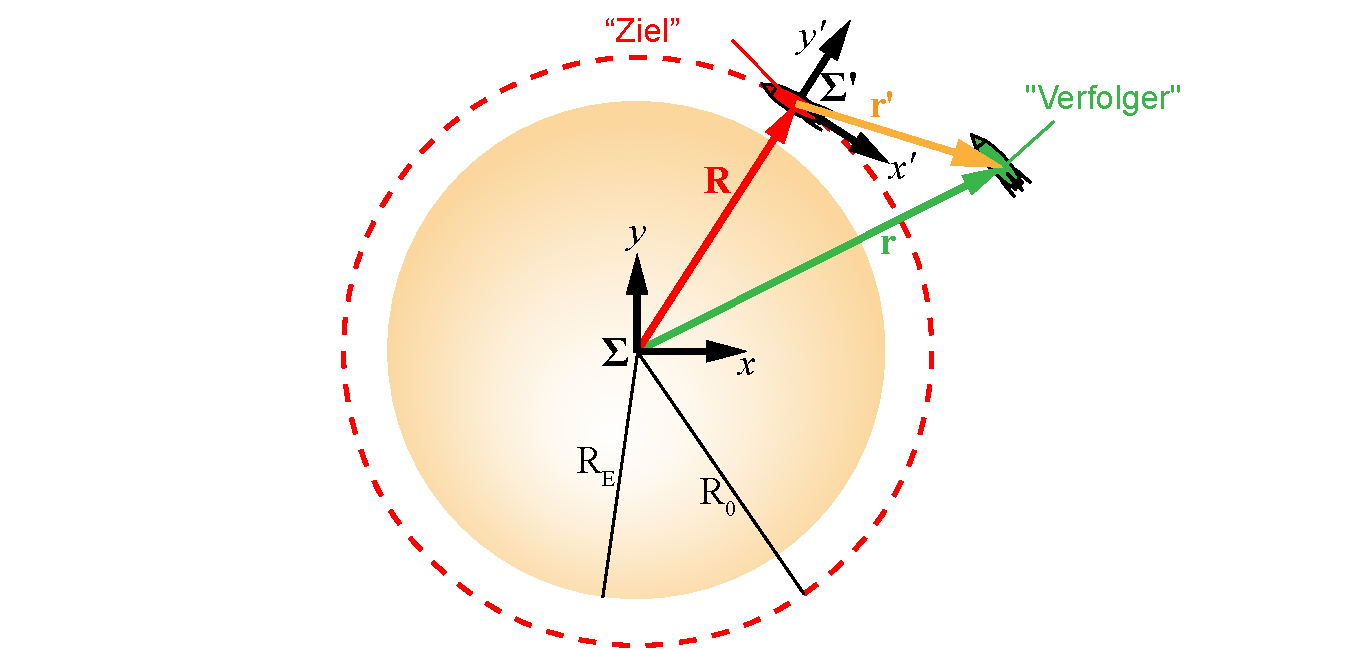
\includegraphics[width=\textwidth]{RendezvousKOS01.pdf} 
	\caption[Koordinatensysteme f�r Rendezvous in der Umlaufbahn.]{Koordinatensysteme f�r Rendezvous in der Umlaufbahn. Wir nehmen zun�chst eine Bewegung der beiden Raumschiffe in der $x$-$y$-Ebene an. Das Inertialsystem $\vec{\Sigma}$ ist in der Erde \bzw dem Mond zentriert, das Nicht-Inertialsystem $\vec{\Sigma}'$ auf dem Ziel-Raumschiff, welches sich mit konstanter Winkelgeschwindigkeit um die Erde \bzw den Mond bewegt. Die $z$-Achse zeigt aus der Papierebene heraus.}
	\label{abb:adyn_rendezvousKOS01}
\end{figure}

Unter Ber�cksichtigung der Gravitationskraft der Erde $\vec{F}_\text{G} =-G\,m_\text{E}\,m_\text{R}\,\vec{r}/ r{}^3 $ und anderer nichtgravitativer Kr�fte $\vec{F}$ (wie \zb Reibung, Schub) ergeben sich dann folgende Bewegungsgleichungen (in drei Dimensionen), wobei $m_\text{R}$ die Masse des Raumschiffs ist:
\begin{align}
\begin{split}
    \ddot{\vec{r}}' &= G\,m_\text{E}\lk\frac{1}{R_0{}^3}-\frac{1}{r^3}\rk\,\vec{r} - \omega_0{}^2\,z'\,\vec{e}_{z'} - 2\vec{\omega}\times\dot{\vec{r}}' + \frac{\vec{F}}{m_\text{R}} \\
    &= \omega_0{}^2 \,\lk 1-\frac{R_0{}^3}{r^3}\rk\,\vec{r} - \omega_0{}^2\,z'\,\vec{e}_{z'} -2\vec{\omega} \times\dot{\vec{r}}' + \frac{\vec{F}}{m_\text{R}} \; .
\end{split}\label{eq:adyn_rendez07}
\end{align}
F�r kleine Abst�nde $r'$ wollen wir diese Gleichung nach $x',\,y',\,z'$ entwickeln und schreiben deshalb den Term mit $1/r^3$ wie folgt:\footnote{Das haben wir ja bereits ausgiebig ge�bt, \zb im \kap{hm_gezeiten}.}
\begin{align}
\begin{split}
    \lk 1-\frac{R_0{}^3}{r^3}\rk\,\omega_0{}^2\,\vec{r} &= \lek 1-\frac{R_0{}^3}{\sqrt{\lk x'{}^2 + \lk R_0+y' \rk^2+z'{}^2\rk^3}}\rek \,\omega_0{}^2\,\lk \vec{r}' + \vec{R} \rk\\
    &= \lek 1-\frac{1}{\sqrt{\lk\lk \frac{x'}{R_0}\rk^2 +\lk 1+\frac{y'}{R_0}\rk^2 + \lk \frac{z'}{R_0}\rk^2\rk^3}}\rek\,\,\omega_0{}^2\,\lk \vec{r}' + R_0\,\vec{e}_{y'}\rk \,.
\end{split} \label{eq:adyn_rendez08}
\end{align}
Wir k�nnen nun $x'/R_0,\,y'/R_0\,,z'/R_0\,\ll\, 1$ annehmen, so dass der Term in der rechteckigen Klammer zu $ \lk 1-\lk 1+2\frac{y'}{R_0}\rk^{-3/2} \rk  = \lk 1-\lk 1-3\frac{y'}{R_0}\rk\rk$ wird und somit aus \eqref{eq:adyn_rendez08}:
\begin{align}
\begin{split}
    \lk 1-\frac{R_0{}^3}{r^3} \rk \, \omega_0{}^2\,\vec{r} 
		&\approx \omega_0{}^2 \lk 3\,\frac{y'}{R_0}\rk \lk x'\,\veceX + y'\,\veceY + z'\,\veceZ + R_0\,\vecpeY\rk \approx 3y' \, \omega_0{}^2 \, \vec{e}_{y'} \,.
\end{split} \label{eq:adyn_rendez09}
\end{align}
Analog l�sst sich zeigen, dass f�r das Kreuzprodukt in \eqref{eq:adyn_rendez07} gilt:
\begin{align}
    -2\vec{\omega}'\times\dot{\vec{r}}' = -2\,\omega_0\,\dot{y}'\,\vecpeX + 2\,\omega_0\,\dot{x}'\,\vecpeY \,. \label{eq:adyn_rendez10}
\end{align}
Damit ergibt sich aus \eqref{eq:adyn_rendez07}:
\begin{align}
    \ddot{\vec{r}}' = 3\,\omega_0{}^2\,y'\,\vec{e}_{y'}  - \omega_0{}^2\,z'\,\vec{e}_{z'}  + 2\,\omega_0\,\dot{x}'\,\vec{e}_{y'}  -2\,\omega_0\,\dot{y}'\,\vec{e}_{x'}  + \frac{\vec{F}}{m_\text{R}}\,. \label{eq:adyn_rendez11}
\end{align}
Man erkennt an \eqref{eq:adyn_rendez11} die verschiedenen Beitr�ge. Der erste Term ist eine Gezeitenkraft, die Terme mit $\dot{x}'$ \bzw $\dot{y}'$ sind Beitr�ge der Coriolis-Kraft. In Komponenten und Matrixform geschrieben wird aus \eqref{eq:adyn_rendez11}:
\begin{align}
    \begin{pmatrix}
        \ddot{x}'\\
        \ddot{y}'\\
        \ddot{z}'
    \end{pmatrix}
    = 2\omega_0
    \begin{pmatrix}
      -\dot{y}'\\
      \dot{x}'\\
      0
    \end{pmatrix}
    +\omega_0^2
    \begin{pmatrix}
        0\\
        3y'\\
        -z'
    \end{pmatrix}
    + \frac{1}{m_\text{R}}
    \begin{pmatrix}
        F_{x'}\\
        F_{y'}\\
        F_{z'}
    \end{pmatrix} \,.\label{eq:adyn_rendez22}
\end{align}
%\begin{align}
    %\begin{pmatrix}
        %\ddot{x}'\\
        %\ddot{y}'\\
        %\ddot{z}'
    %\end{pmatrix}
%=
    %\begin{pmatrix}
       %-2\,\omega_0\,\dot{y}'\\
        %2\,\omega_0\,\dot{x}' + 3\,\omega_0{}^2\,y' \\
        %-\omega_0{}^2\,z'
    %\end{pmatrix} \,+ \,
		%\begin{pmatrix}
       %F_{x'}/m_\text{R}\\
       %F_{y'}/m_\text{R}\\
       %F_{z'}/m_\text{R}
    %\end{pmatrix} \, . \label{eq:adyn_rendez12a}
%\end{align}
%\begin{subequations}
%\begin{align}
    %\ddot{x}' &= -2\,\omega_0\,\dot{y}' + \frac{F_{x'}}{m_\text{R}} \,,\\
    %\ddot{y}' &= 2\,\omega_0\,\dot{x}' + 3\,\omega_0{}^2\,y'+ \frac{F_{y'}}{m_\text{R}}\,,\\
    %\ddot{z}' &= -\omega_0{}^2\,z' + \frac{F_{z'}}{m_\text{R}}\,.
%\end{align}\label{eq:adyn_rendez12}
%\end{subequations}
Diese Gleichungen werden in der Literatur als \emph{Hill\footnote{George William Hill (1838--1914) war ein US-amerikanischer Astronom und Mathematiker, dessen Methoden zur Bahnberechnung von Himmelsk�rpern bis heute u.a. auch in der Raumfahrt verwendet werden.}-Gleichungen}\index{Hill-Gleichungen}\indexp{Hill, George William} bezeichnet. \\
Wir wollen diese nun unter der Annahme impulsiver Man�ver l�sen, so dass wir $F_{x'}$, $F_{y'}$, $F_{z'}$ alle gleich Null setzen k�nnen. Die Gleichung f�r $\ddot{z}'(t)$ ist vollkommen von den anderen Gleichungen entkoppelt und man erh�lt sofort f�r $z'\lk t\rk$ die L�sung 
\begin{align}
\begin{split}
    z'\lk t\rk &= z_0'\,\cos\lk \omega_0 t\rk + \frac{\dot{z}_0'}{\omega_0}\,\sin\lk \omega_0 t\rk, \\
    \dot{z}'\lk t\rk &= -z_0'\,\omega_0\,\sin\lk \omega_0 t\rk + \dot{z}_0'\,\cos\lk \omega_0 t\rk \,.
\end{split}  \label{eq:adyn_rendez13}
\end{align} 
Das bedeutet, dass das Raumschiff in $z'$-Richtung eine harmonische Bewegung ausf�hrt, deren Periode durch die Umlaufzeit $T_0 = 2\pi/\omega_0=2\pi\sqrt{R_0{}^3/(G m_\text{E})}$ des Ziels definiert ist. Das bedeutet aber auch, dass durch die entsprechende Wahl von $z_0'$ und $\dot{z}_0'$ diese Bewegung so kompensiert werden kann, dass das Rendezvous-Man�ver nur in der $x',y'$-Ebene stattfindet und dort betrachtet werden muss. In dieser Ebene gibt es nun ein interessantes Wechselspiel von Gezeiten- und Coriolis-Kraft. \\
Wir wollen die Hill-Gleichungen \eqref{eq:adyn_rendez22} weiter l�sen und nehmen die Anfangsbedingungen $x_0'$, $\dot{x}_0'$, $y_0'$ und $\dot{y}_0'$ als gegeben an. Die L�sung erfolgt �hnlich zu der, die in Kapitel 1.3.2 in Band I f�r die Bewegungsgleichungen eines Massepunktes im \KOS\ der rotierenden Erde gezeigt wurde. Wir erhalten anstelle der zwei Differentialgleichungen zweiter Ordnung nun vier Differentialgleichungen erster Ordnung:
\begin{subequations}
\begin{align}
    x'\lk t\rk = &\lk 6\,y_0' +4\,\frac{\dot{x}_0'}{\omega_0}\rk\,\sin\lk \omega_0 t\rk + \frac{2\dot{y}_0'}{\omega_0}\,\cos\lk \omega_0 t\rk + x_0' -2\,\frac{\dot{y}_0'}{\omega_0} - \lk 6\,\omega_0\,y_0' + 3\,\dot{x}_0'\rk\,t\,, \label{eq:adyn_rendez14a} \\
\dot{x}'\lk t\rk = &\lk 6\,\omega_0\,y_0' +4\,\dot{x}_0'\rk\,\cos\lk\omega_0 t\rk - 2\,\dot{y}_0'\,\sin\lk\omega_0t\rk - 6\,\omega_0\,y_0'-      3\,\dot{x}_0' \,, 
\label{eq:adyn_rendez14b} \\
y'\lk t\rk = &-\lk 3\,y_0' +2\,\frac{\dot{x}_0'}{\omega_0}\rk\,\cos\lk \omega_0 t\rk + \frac{\dot{y}_0'}{\omega_0}\,\sin\lk \omega_0 t\rk + 4\,y_0' + 2\,\frac{\dot{x}_0'}{\omega_0} \,, \label{eq:adyn_rendez14c} \\
\dot{y}'\lk t\rk = &\lk 3\,\omega_0\,y_0' +2\,\dot{x}_0'\rk\,\sin\lk\omega_0 t\rk + \dot{y}_0'\,\cos\lk\omega_0t\rk \,. \label{eq:adyn_rendez14d}
\end{align} 
\end{subequations}
Diese Gleichungen zusammen mit \eqref{eq:adyn_rendez13} hei�en \gls{CWG}\index{Clohessy-Wiltshire-Gleichungen|textbf}\footnote{Diese Gleichungen wurden erstmals im Jahre 1960 im Zusammenhang mit dem Mercury Programm der NASA ver�ffentlicht.} und beschreiben die Bewegung eines Raumschiffs im Koordinatensystem des Ziels, dem sich der Verfolger ann�hern will. Sie sind die L�sungen der Bewegungsgleichung f�r den Verfolger im mitbewegten Koordinatensystem, die man nat�rlich auch numerisch aus dem DGL-System \eqref{eq:adyn_rendez22} der Hill-Gleichungen mittels \matlab{} berechnen kann (siehe \probref{adyn_rendezvous01}). Sie zeigen durch das Zusammenwirken von Gezeitenkraft und Coriolis-Kraft einige Besonderheiten in den Ann�herungstrajektorien, die gerade in der Fr�hphase der bemannten Raumfahrt f�r �berraschung sorgten. Man beachte insbesondere die direkte lineare Zeitabh�ngigkeit in \eqref{eq:adyn_rendez14a}.\\
Auch die L�sungen der Clohessy-Wiltshire-Gleichungen lassen sich vorteilhaft in der Matrix-Form schreiben (hier f�r den im kr�ftefreien Fall):
\begin{align}
\begin{split}
    \begin{pmatrix}
        x'\\
        y'\\
        z'
    \end{pmatrix}
    = \,&\frac{\sin\omega_0 t}{\omega_0}
    \begin{pmatrix}
        4\dot{x}_0'+6\omega_0 y_0\\
        \dot{y}_0' \\
        \dot{z}_0'
    \end{pmatrix}
    + \frac{\cos\omega_0 t}{\omega_0}
    \begin{pmatrix}
        2\dot{y}_0'\\
        -2\dot{x}_0' -3\omega_0 y_0'\\
        \omega_0 z_0'
    \end{pmatrix} 
    - t
    \begin{pmatrix}
        6\omega_0 y_0' + 3\dot{x}_0'\\
        0\\
        0
    \end{pmatrix}+\frac{1}{\omega_0}
    \begin{pmatrix}
        1\omega_0 x_0' - 2\dot{y}_0'\\
        4\omega_0 y_0' + 2\dot{x}_0'\\
        0 
    \end{pmatrix} \,, 
\end{split} \label{eq:adyn_rendez23}
\end{align}
worin $x_0'$, $y_0'$, $z_0'$ die Anfangspositionen und $\dot{x}_0'$, $\dot{y}_0'$, $\dot{z}_0'$ die Anfangsgeschwindigkeiten des Verfolgers relativ zum Ziel sind.\\
Gibt man bei vorgegebenen Anfangswerten eine Zeit $t_\text{K}$ bis zum Zusammentreffen von Verfolger und Ziel vor (Kopplung), dann kann man aus \eqref{eq:adyn_rendez23} die notwendigen Anfangsgeschwindigkeiten berechnen, die der Verfolger haben muss, damit das Rendezvous gelingen kann:
\begin{align}
    \begin{pmatrix}
        \dot{x}_0'\\ \\
        \dot{y}_0'\\ \\
        \dot{z}_0'
    \end{pmatrix}
    &= 
    \begin{pmatrix}
        C(t_\text{K})\cdot\lek x_0'\,\omega_0\,\sin\omega_0 t_\text{K} + y_0'\,\omega_0\,\lk 6\,\omega_0\, t_\text{K}\,\sin\omega_0  t_\text{K} - 14 + 14\cos\omega_0  t_\text{K}\rk \rek \\ \\
        C(t_\text{K})\cdot\lek 2\,x_0'\,\omega_0\,\lk 1-\cos\omega_0  t_\text{K}\rk + y_0'\,\omega_0\, \lk 4\,\sin\omega_0 t_\text{K} \linebreak -3\,\omega_0 t_\text{K}\,\cos\omega_0 t_\text{K} \rk \rek\\ \\
			 - \omega_0\,z_0'/\tan\lk\omega_0 t_\text{K}\rk
    \end{pmatrix}  \label{eq:adyn_rendez24} \\
		\text{mit} ~~ C(t_\text{K}) &= \lek 3\,\omega_0\, t_\text{K}\,\sin\omega_0  t_\text{K} - 8\,\lk 1- \cos\omega_0  t_\text{K}\rk \rek^{-1}\,. \nonumber
\end{align}
Wir leiten noch eine Beziehung f�r die Energie des Verfolgers im \KOS\ des Ziels her. 
Da die Coriolis-Kraft immer senkrecht zur Bewegungsrichtung  ist, leistet sie keine Arbeit. Die einzige Kraft, die in \eqref{eq:adyn_rendez22} dann Arbeit leisten kann ist die Gezeitenkraft entlang der $y'$-Koordinate. 
Es ergibt sich damit f�r die Energie des Verfolger im \KOS\ des Ziel:
\begin{align}
    E &= T + U = \frac{1}{2}\,m_\text{R}\,\lk \dot{x}'^2 + \dot{y}'^2\rk -\int_0^{y'} F\D \tilde{y} = \frac{1}{2}\,m_\text{R}\,\lk \dot{x}'^2+\dot{y}'^2\rk -m_\text{R}\,3\,\omega_0\,\int\limits_0^{y'} \tilde{y}\D \tilde{y} \nonumber \\
    &= \frac{1}{2}\,m_\text{R}\,\lek \dot{x}'^2+\dot{y}'^2 - 3\,\omega_0\,y'^2\rek = \con \,.  \label{eq:adyn_rendez25}
\end{align}
Wir k�nnen daraus absch�tzen, ab welchem relativen Abstand $y'$ zwischen Ziel und Verfolger die Geschwindigkeit des Verfolgers durch die Gezeitenkraft merklich ver�ndert wird. Da $\omega_0 = 2\pi/T_\text{K} \approx 2\pi / \SI{1}{\hour} \approx 2\pi/\SI{3600}{\second} \approx \SI{e-3}{\radian\per\second}$ muss $y'\leq \SI{1}{\km}$ sein, damit $v= \sqrt{\dot{x}'^2+\dot{y}'^2}$ sich merklich, \dh um $\approx \SI{1}{\metre\per\second}$, �ndert. Anders gesagt: Man muss die Clohessy-Wiltshire-Gleichungen\index{Clohessy-Wiltshire-Gleichungen} erst ab Relativabst�nden von $<\SI{1}{\km}$ ber�cksichtigen, ansonsten kann man rechnen, als ob die Bewegung in einem Inertialsystem stattfindet. Wir wollen nun die R�ckkehr eines Astronauten zu seinem Mutterschiff (\zb der ISS) behandeln.
%NEBEBENRECHNUNG %%%%%%%%%%%%%%%%%%%%%%%%%%%%%%%%%%%%%%%%%%%%%%%%%%%%%%%%%%%%%%%%%%%%%%%%%%
%
%\begin{nebenrechnungNeu} {Clohessy-Wiltshire-Gleichungen}
%
%Wir starten von der Darstellung \eqref{eq:adyn_rendez23}:
%\begin{align}
%\begin{split}
    %\omega\,x &= \lk 6 \omega\, y_0 + 4\dot{x}_0\rk\,  \sin \omega t + 2 \dot{y}_0 \, \cos \omega t + \omega t \, \lk -6 \omega\,  y_0 - 3 \dot{x}_0\rk  + \omega\,  \lk x_0 - 2 \dot{y}_0\rk\,,  \\
    %\omega \, y &= \lk \dot{y}_0\rk \,  \sin \omega t + \lk -3 \omega \, y_0 - 2 \dot{x}_0\rk \,  \cos \omega t + \omega \, \lk 4 y_0 + 2 \dot{x}_0\rk  \, ,\\
    %\omega \, z &= \dot{z}_0\, \sin \omega t + \omega\,  z_0 \, \cos \omega t +0
%\end{split}\label{eq:adyn_CWEq_01}
%\end{align}
%
%Umordnung nach $\dot{x}_0, \dot{y}_0, \dot{z}_0$ und $x = y = z = 0$:
%
%\begin{align}
%\begin{split}
    %\begin{pmatrix} 0 \\ 0 \\ 0 \end{pmatrix} =\,
    %&\underbrace{\begin{pmatrix} 4 \sin \omega t - 3 \omega t & 2 \cos \omega t - 2 & 0 \\
    %-2 \cos \omega t + 2 & \sin \omega t & 0 \\
    %0 & 0 & \sin \omega t 
    %\end{pmatrix} }_{\substack{\hat{A}}}
    %\begin{pmatrix} \dot{x}_0 \\ \dot{y}_0 \\ \dot{z}_0 \end{pmatrix} 
    %\\ &+ \underbrace{\begin{pmatrix} 6 \omega \,y_0\, \sin \omega t - 6 \omega^2 t\,y_0 + \omega x_0 \\
    %-3 \omega \,y_0\, \cos \omega t + 4 \omega\, y_0 \\
    %\omega\, z_0\, \cos \omega t 
    %\end{pmatrix}}_{\substack{-\hat{B}}}
%\end{split}\label{eq:adyn_CWEq_02}
%\end{align}
%\begin{align}
    %-\hat{B} &= \omega \, 
    %\begin{pmatrix}
        %6 y_0\,\sin \omega t - 6 \omega t \,y_0 + x_0 \\ 
        %-3 y_0\, \cos \omega t + 4 y_0 \\ 
        %z_0\, \cos \omega t 
    %\end{pmatrix} \label{eq:adyn_CWEq_03}\\
    %\rightarrow \quad \hat{B} &= \omega \,
    %\begin{pmatrix}
        %-6 y_0 \,\sin \omega t + 6 \omega t\, y_0 - x_0 \\ 
        %3 y_0\, \cos \omega t - 4 y_0 \\ 
        %-z_0\, \cos \omega t 
    %\end{pmatrix} \label{eq:adyn_CWEq_04}\\
  %\rightarrow\quad  \hat{B} &=      \hat{A} \hat{X}\nonumber\\
    %\rightarrow\quad \hat{X} &= 
    %\begin{pmatrix} 
        %\dot{x}_0 \\ 
        %\dot{y}_0 \\ 
        %\dot{z}_0 
    %\end{pmatrix} 
    %= \hat{A}^{-1}\, B\label{eq:adyn_CWEq_05}
%\end{align}
%\subsubsection*{Cramersche Regel}
%\begin{align}
    %\dot{x}_0 &= \frac{\det \hat{A}_x}{\det \hat{A}}, \quad
    %\dot{y}_0 = \frac{\det \hat{A}_y}{\det \hat{A}}, \quad
    %\dot{z}_0 = \frac{\det \hat{A}_z}{\det \hat{A}}\label{eq:adyn_CWEq_06}
%\end{align}
%\begin{align}
    %\det \hat{A} &= 
    %\begin{vmatrix}
        %\lk 4 \sin \omega t - 3 \omega t \rk & -2\, \lk 1 - \cos \omega t \rk & 0 \\
        %+2 \,\lk 1 - \cos \omega t \rk & \sin \omega t & 0 \\
        %0 & 0 & \sin \omega t
    %\end{vmatrix} \label{eq:adyn_CWEq_07}
%\end{align}
%\begin{align*}
    %&= \lk 4 \sin \omega t - 3 \omega t \rk\, \sin^2 \omega t + 4 \sin \omega t \,\lk 1 - \cos \omega t \rk^2\\
    %&= \sin \omega t \,
    %\lk 4 \sin^2 \omega t - 3 \omega t \,\sin \omega t + 4 + 4 \cos^2 \omega t - 8 \cos \omega t \rk\\
    %&= \sin \omega t \,
    %\lek 8 \,\lk 1 - \cos \omega t \rk - 3 \omega t\, \sin \omega t \rek
%\end{align*}
%\begin{align}
    %\det \hat{A}_z &=
    %\begin{vmatrix}
         %4 \sin \omega t - 3 \omega t & -2 \,\lk 1 - \cos \omega t \rk & -6 \omega \,y_0\, \sin \omega t + 6 \omega^2 t\, y_0 - \omega \,x_0 \\
        %2 \,\lk 1 - \cos \omega t \rk & \sin \omega t & -3 \omega \,y_0\, \cos \omega t - 4 \omega \,y_0 \\
        %0 & 0 & -\omega \,z_0\, \cos \omega t
    %\end{vmatrix}\\
    %&= -\lk 4 \sin \omega t - 3 \omega t \rk \,\sin \omega t \,\omega \,z_0 \,\cos \omega t - 4 \omega \,z_0 \,\cos \omega t \,\lk 1 - \cos \omega t \rk^2\nonumber\\
    %&= -\cos \omega t \,\omega \,z_0 \,
    %\lk 4 \sin^2 \omega t - 3 \omega t \,\sin \omega t + 4 + 4 \cos^2 \omega t - 8 \cos \omega t \rk \nonumber\\
    %&= -\cos \omega t \,\omega \,z_0 \,
    %\lek 8 \,\lk 1 - \cos \omega t \rk - 3 \omega t \,\sin \omega t \rek \nonumber\\
    %\rightarrow \quad \dot{z}_0 &= - \frac{\cos \omega t\, \omega\, z_0}{\sin\omega t} = -\frac{\omega\,z_0}{\tan\omega t}\label{eq:adyn_CWEq_09}
%\end{align}
%\begin{align}
    %\det \hat{A}_x &=
    %\begin{vmatrix}
        %6 \omega \,y_0\, \sin \omega t - 6 \omega^2 \,t \,y_0 + \omega \,x_0 & -2 \,\lk 1 - \cos \omega t \rk & 0 \\
        %-3 \omega\, y_0\, \cos \omega t + 4 \omega\, y_0 & \sin \omega t & 0 \\
        %\omega\, z_0\, \cos \omega t & 0 & \sin \omega t
    %\end{vmatrix}\label{eq:adyn_CWEq_10}
%\end{align}
%
%\end{nebenrechnungNeu}
%
%%%%%%%%%%%%%%%%%%%%%%%%%%%%%%%%%%%%%%%%%%%%%%%%%%%%%%%%%%%%%%%%%%%%%%%%%%%%%%%%%%%%%%%%%%%%
%BEISPIEL 1 %%%%%%%%%%%%%%%%%%%%%%%%%%%%%%%%%%%%%%%%%%%%%%%%%%%%%%%%%%%%%%%%%%%%%%%%%%%%%%%%%
\begin{example}{R�ckkehr eines Astronauten zur Raumstation}  
Wir nehmen folgende Parameter an: 
\begin{align*}
    h_\text{ISS} &= \SI{420.0}{\km}\,, ~ R_0 = \SI{6778}{\km} \,,~
    T_\text{P}   = \SI{ 92.4}{\min}\,, ~ \omega_0 = \SI{1.13e-3}{\radian\per\second}\,,~  x_0' = y_0' = \SI{100}{\metre}\,, ~\dot{x}_0' = \dot{y}_0' = 0\,.
\end{align*}
\begin{enumerate}
    \item [a)]
    Was passiert, wenn der Astronaut \anf{nichts} macht?
    \begin{align}
        x'\lk t\rk &= x_0'-6\,y_0'\,\lek\omega_0 t - \sin\lk\omega_0 t\rk\rek\,, ~~~ y'\lk t\rk = y_0' +3\,y_0'\,\lek 1-\cos\lk\omega_0t\rk\rek\,. \label{eq:adyn_rendez26}
    \end{align}
    Der Astronaut wird sich durch die Gezeitenkraft in $x'$-Richtung immer weiter von der ISS entfernen und dabei durch die Coriolis-Kraft in $y'$-Richtung eine Art schwingende Bewegung ausf�hren (\figref{adyn_rendezvous02}).
		
	\begin{figure}[H]
	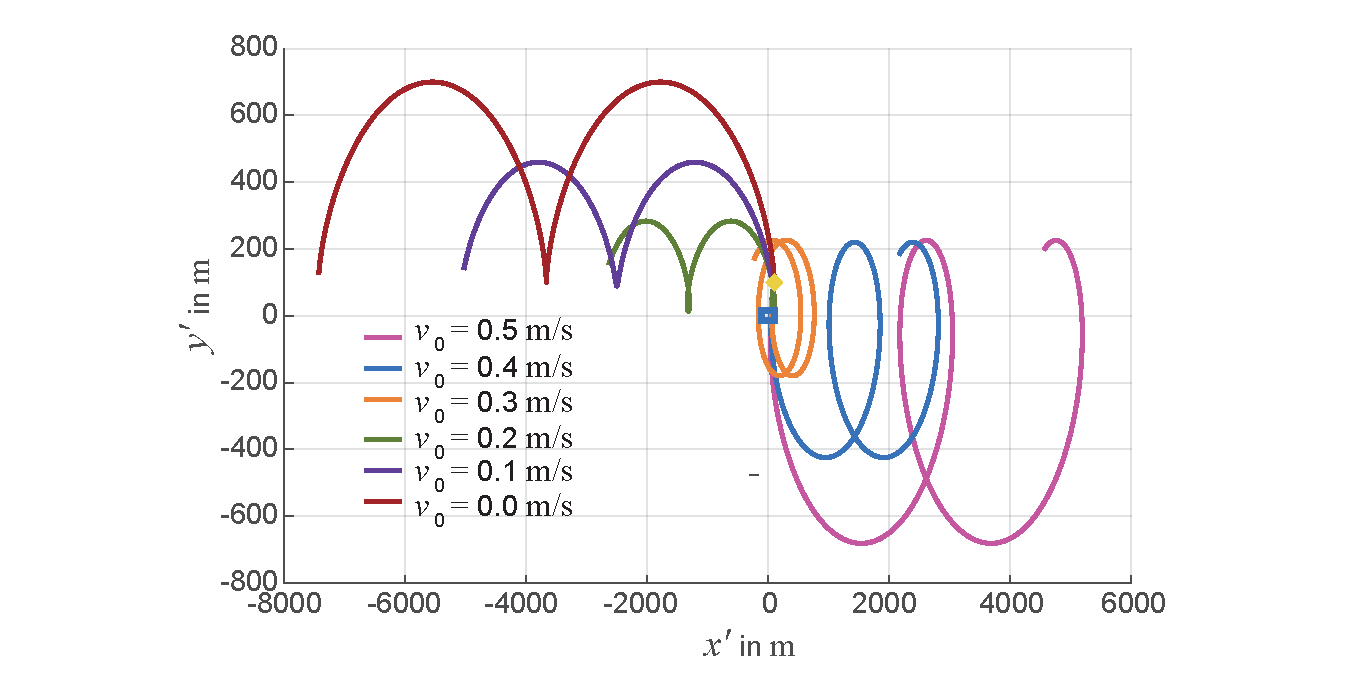
\includegraphics[width=\textwidth]{RendezvousAstronaut01.pdf} 
	\caption[Astronaut au�erhalb der ISS.]{Astronaut au�erhalb der ISS. Der Astronaut befindet sich initial bei $x_0'=y_0'=\SI{100}{\metre}$ und bewegt sich mit einer Anfangsgeschwindigkeit $v_0$ (also keine initiale Relativgeschwindigkeit zum Ziel, d.h. $\dot{x}_0'=\dot{y}_0=0'$) genau in Richtung auf die Station zu. Selbst bei $v_0=0$ entfernt sich der Astronaut mit der Zeit von der Raumstation. Dargestellt sind die L�sungen der Clohessy-Wiltshire-Gleichungen wie im \mscr~ \mladynref{Rendezvous01.m} im Detail ausgef�hrt.}
	\label{abb:adyn_rendezvous02}
\end{figure}

  \item[b)]
    Was passiert, wenn der Astronaut seinen R�ckkehrantrieb (englisch \textit{Return-Thruster}) mit einem Antriebsverm�gen von $\SI{1}{\metre\per\second}$ einsetzt?   
		Intuitiv \anf{zielt} der Astronaut mit seinem auf dem R�cksto�-Prinzip basierenden Thruster genau in Richtung ISS, also mit
    \begin{align*}
        \vec{v}_0 = 
        \begin{pmatrix}
            \dot{x}_0'\\
            \dot{y}_0'\\
            \dot{z}_0'
        \end{pmatrix}
        = \frac{1}{\sqrt{2}}
        \begin{pmatrix}
            1\\
            1\\
            0
        \end{pmatrix}
        \SI{}{\metre\per\second}\,.
    \end{align*}
    Leider wird durch die kombinierte Wirkung der Gezeiten und Coriolis-Kraft der Astronaut die ISS verfehlen, wie Gleichung \eqref{eq:adyn_rendez23} und \figref{adyn_rendezvous02} und \figref{adyn_rendezvous03}a zeigen.\\
    \item[c)]
    Wie muss der Astronaut beim Abfeuern seines Thrusters zielen, damit er die ISS sicher erreicht? \\
		$\dot{x}_0'$, $\dot{y}_0'$ ergeben sich aus \eqref{eq:adyn_rendez24}. Wir k�nnen noch eine kleine Eigengeschwindigkeit des Astronauten vor dem Starten des Thrusters mit $\vec{v}_\text{vor} = \lk\dot{x}_{\text{vor},0'}, \dot{y}_{\text{vor},0'}\rk$ annehmen und erhalten den richtigen Zielwinkel:
    \begin{align}
        \tan\lk\gamma\rk = \frac{\Delta v_y}{\Delta v_x} = \frac{\dot{y}_0' -\dot{y}_{\text{vor},0'}}{\dot{x}_0'- \dot{x}_{\text{vor},0'}} \,. \label{eq:adyn_rendez27}
    \end{align}
\end{enumerate}
In der Realit�t wird sich der Astronaut nat�rlich in kleinen Minisch�ben iterativ der ISS n�hern, doch auch daf�r gelten die abgeleiteten Formeln.

\begin{figure}[H]
	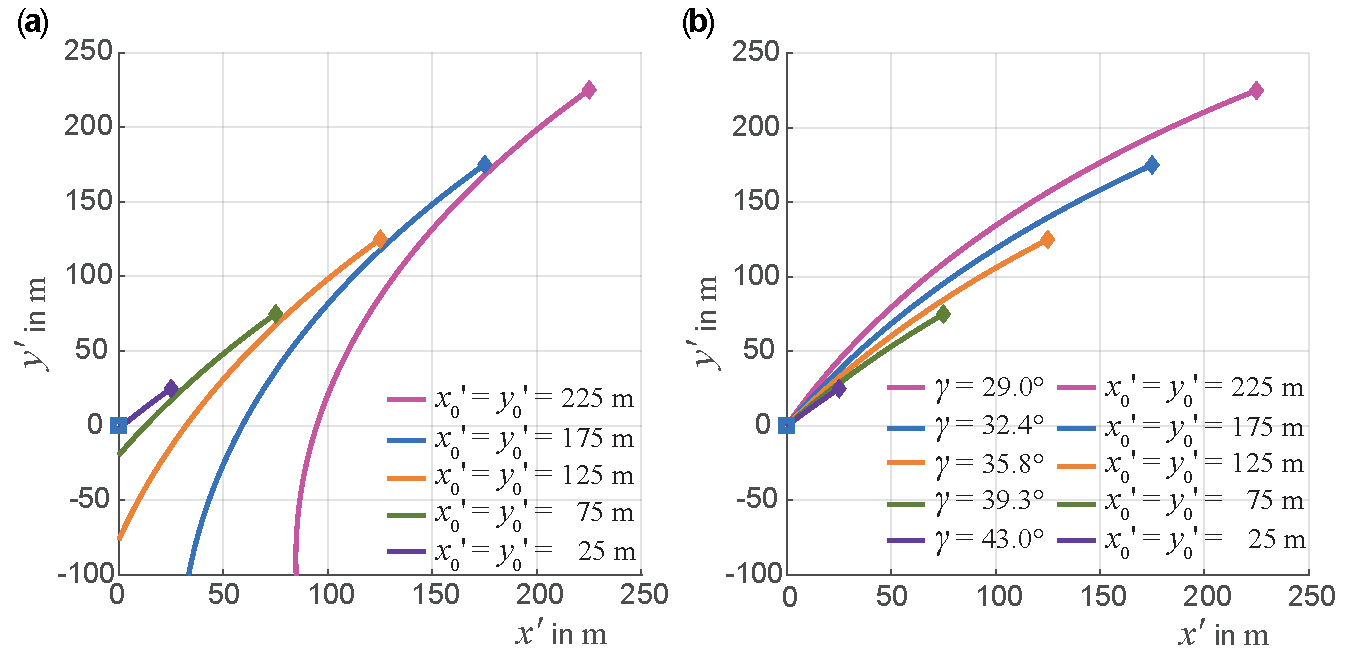
\includegraphics[width=\textwidth]{RendezvousAstronaut02.pdf} 
	\caption[Astronaut au�erhalb der ISS.]{Astronaut au�erhalb der ISS. \fa Der Astronaut befindet sich initial bei $x_0'=y_0'=\SI{25}{\metre} \ldots \SI{225}{\metre}$ und "`zielt"' mit seinem Antriebssystem  mit einer Anfangsgeschwindigkeit $v_0$ genau in Richtung auf die Station. L�sung der Hill-Gleichungen. \fb Der Astronaut befindet sich ebenfalls initial bei $x_0'=y_0'=\SI{25}{\metre} \ldots \SI{225}{\metre}$ und bewegt sich mit einem optimierten Zielwinkel $\gamma$ der Richtung Anfangsgeschwindigkeit von $v_0 = \SI{1}{\metre\per\second}$ auf die Station zu (L�sung der Clohessy-Wiltshire-Gleichungen\index{Clohessy-Wiltshire-Gleichungen}). Offensichtlich wird der Astronaut erst bei Entfernung von kleiner als 50 m bei direkter Anzielung der Station auch bei dieser wirklich ankommen. Die Rechnungen sind im \mscr~ \mladynref{Rendezvous02.m} im Detail ausgef�hrt.}
	\label{abb:adyn_rendezvous03}
\end{figure}

\label{bsp:adyn_stranded_astronaut}
\end{example}
%BEISPIEL %%%%%%%%%%%%%%%%%%%%%%%%%%%%%%%%%%%%%%%%%%%%%%%%%%%%%%%%%%%%%%%%%%%%%%%%%%%%%%%%%%

\subsection{Rendezvous Space Shuttle und ISS}\label{kap:adyn_rendezvous_ISS}

Ganz analog zu den Rechnungen im vorhergehenden Kapitel kann man das Weltraum-Rendezvous von einem Raumtransporter und der ISS berechnen. 
Wenn zwei Raumschiffe vor einer Kopplung f�r l�ngere Zeit in einem konstanten Abstand fliegen sollen, ist dies ohne st�ndigen Treibstoffverbrauch nur m�glich, wenn sich beide in der gleichen Umlaufbahn befinden. Ist dies nicht der Fall,  wird der Verfolger vom Ziel aus gesehen eine Ellipsenbahn (\bzw ellipsen�hnliche Bahn) beschreiben, die man sich leicht �ber die Berechnung im Inertialsystem aus den Kepler-Bahnen beschaffen kann. Dabei muss man ber�cksichtigen, dass das Koordinatensystem $\vec{\Sigma}'$ in der Zeit mitgedreht werden muss, denn die $y'$-Achse soll ja immer radial nach au�en zeigen.
Zur Berechnung der von der ISS beobachteten Bahnen �ber die Hill- \bzw CW-Gleichungen muss man neben den Anfangskoordinaten $\vec{r}_0,\, \vec{R}_0$ auch die Anfangsgeschwindigkeiten $\vec{v}_0,\, \vec{V}_0$, sowie deren Umrechnung in das mitbewegte \KOS\ der ISS (des Ziels) kennen. 
\begin{figure}[H]
	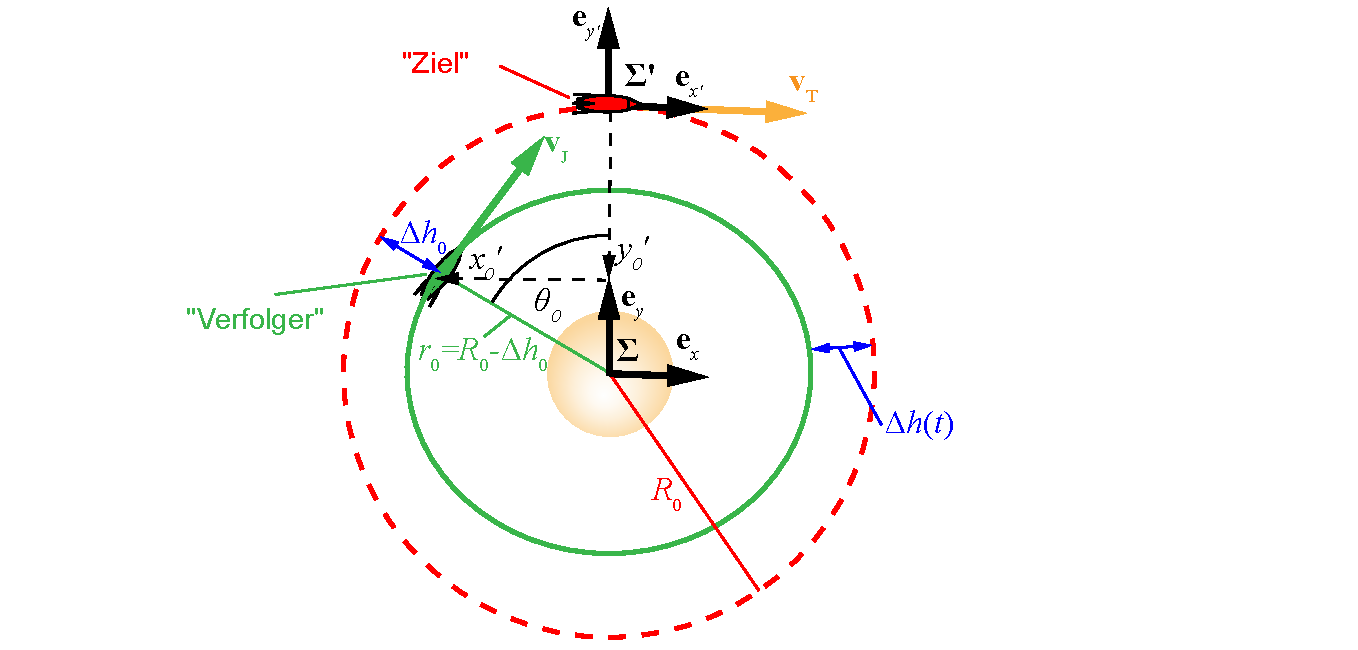
\includegraphics[width=\textwidth]{RendezvousKOS02.pdf} 
	\caption[Koordinatensysteme f�r Rendezvous in der Umlaufbahn.]{Koordinatensysteme f�r Rendezvous in der Umlaufbahn. Wir nehmen eine Bewegung der beiden Raumschiffe in der $x$-$y$-Ebene an. Die $z$-Achse zeigt aus der Papierebene heraus. F�r das Ziel wird vereinfachend eine Kreisbahn angenommen, der Verfolger befindet sich auf einer elliptischen Bahn. Ebenfalls wurde vereinfachend angenommen, dass zum Zeitpunkt $t=0$ die Achsen $\veceY,\, \vecpeY$ in die gleiche Richtung zeigen und $\veceY$ auch zum Perig�um der Bahn des Verfolgers.}
	\label{abb:adyn_rendezvousKOS02}
\end{figure}
Die Situation ist in \figref{adyn_rendezvousKOS02} gezeigt. Man liest f�r die Anfangsbedingungen ab:
	\begin{align}
	\begin{split}
		\vec{r}_0 &= x_0\, \veceX + y_0\,\veceY \,, \\
		\vec{R}_0 &= (0,R_0)\,, \\
		\vec{r}_0' &= x_0'\, \vecpeX + y_0'\,\vecpeY \,.
		\end{split} \label{eq:adyn_rendez28}
	\end{align}
Die beiden Vektoren $\vec{R}_0,\,\vec{r}_0$ bilden einen Winkel $\theta_0$, der sich mit $\Delta h_0 =\Delta h(t_0)$ aus
	\begin{align}
		\sin\theta_0 &= -\frac{x_0'}{R_0-\Delta h_0} ~~~\text{\bzw}~~~ \cos\theta_0 = -\frac{R_0+y_0'}{R_0-\Delta h_0}\, \label{eq:adyn_rendez29}
	\end{align}
bestimmen l�sst. F�r die Anfangsgeschwindigkeiten finden wir:
	\begin{align}
	\begin{split}
		\vec{V}_0 \,=\,&\dot{\vec{R}}_0 \,= \,R_0\,\omega_\text{T} \,\veceX\,,\\
		\vec{v}_0 \,=\,&\dot{\vec{r}}_0 \,= \,v_{\text{J},0} \lk \cos\theta_0\,\veceX + \sin\theta_0\,\veceY \rk\,.\\
	\end{split}  \label{eq:adyn_rendez30}
	\end{align}
Befindet sich der Verfolger auch auf einer Kreisbahn mit dem Radius $R_0-\Delta h_0$, dann ist $ v_{\text{J},0} = \omega_\text{J}\,(R_0-\Delta h_0)=\sqrt{G m_\text{M}/(R_0-\Delta h_0)}$, ansonsten bestimmt sich $v_{\text{J},0}$ aus der L�sung der Kepler-Gleichung \bzw der \gls{visvivaadyn} \eqref{eq:hm_vis-viva}. 
F�r einen solchen Fall nehmen wir eine Bahn des Verfolgers mit einer Exzentrizit�t $e$ und einer gro�en Halbachse $a=R_0$ an. Zum Zeitpunkt $t=0$ sollen sich Ziel und Verfolger bei $(0,0)\,\bzw (0,y_0')$ befinden. Dann ist 
\begin{align}
  \vec{v}_0 &= v_{\text{J},0} \,\veceX ~~~\text{mit}~~~v_{\text{J},0} = \sqrt{\frac{G\,m_\text{E}}{R_0}}\,\sqrt{\frac{1+e}{1-e}} \approx (1+e)\,R_0\,\omega_\text{T} \, \veceX \,. \label{eq:adyn_rendez30a}
\end{align}
Hat der Verfolger bereits im Inertialsystem eine Anfangsgeschwindigkeit $\vec{v}_0 \neq 0$, so m�ssen wir f�r die L�sung der Hill- \bzw die Nutzung der CW-Gleichungen, die sich daraus im mitbewegten \KOS\ $\vec{\Sigma}'$ ergebende Anfangsgeschwindigkeit $\vec{r}_0'$ kennen. Diese berechnet sich nach \eqref{eq:adyn_rendez04} zu:
	\begin{align}
		\dot{\vec{r}}_0' &= \dot{\vec{r}}'(t=0)= \dot{\vec{r}}_0 - \dot{\vec{R}}_0 - \vec{\omega}_0' \times \vec{r}'_0 = \vec{v}_0 - \vec{V}_0 - \vec{\omega}_0' \times \vec{r}'_0  \,. \label{eq:adyn_rendez31}
	\end{align}
Hierin ist $\vec{\omega}_0'$ der Rotationsvektor f�r die Drehung des mitbewegten Koordinatensystems, welches sich mit der Bewegung des Ziels so dreht, dass die $\vecpeY$-Achse immer radial nach au�en zeigt.

\begin{figure}[H]
	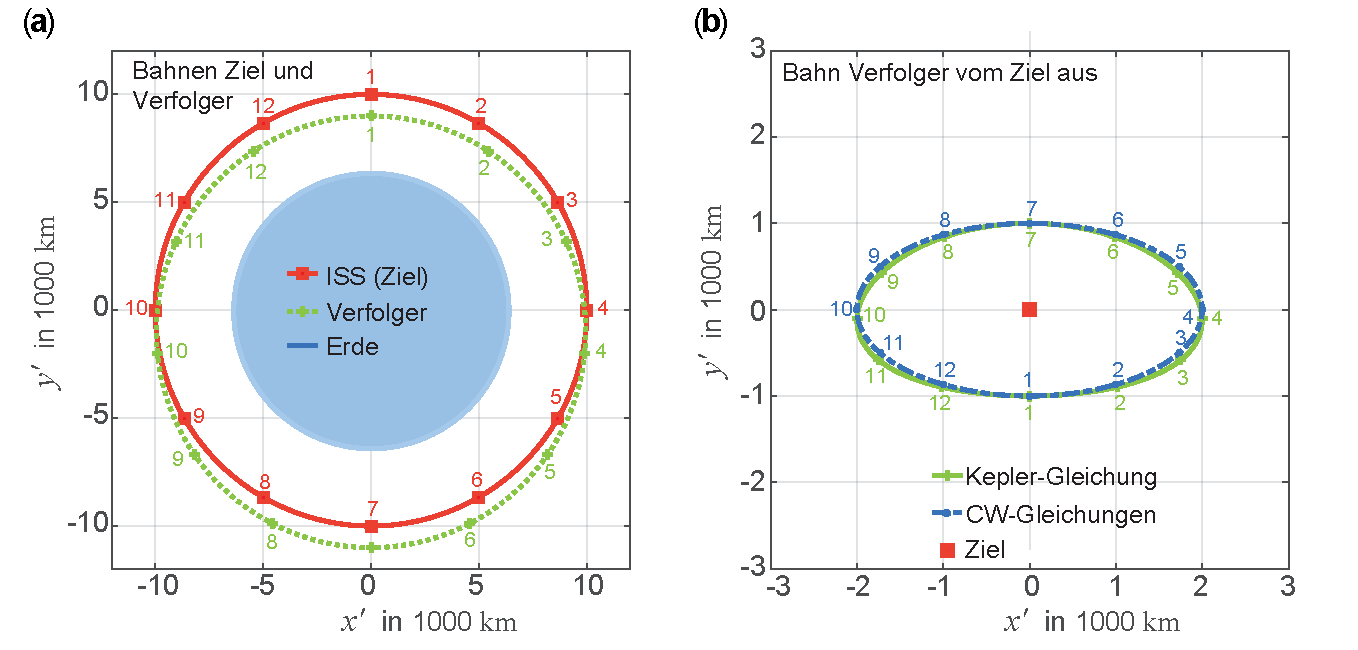
\includegraphics[width=\textwidth]{Raumschiff2Orbits.pdf} 
	\caption[Zwei Raumschiffe in unterschiedlichen Umlaufbahnen.]{Zwei Raumschiffe in unterschiedlichen Umlaufbahnen.\fa Bahnen von Ziel und Verfolger im Inertialsystem. \fb Bahn Verfolger von Ziel aus. L�sungen nach der Kepler-Gleichung mit Drehung des mitbewegten Koordinatensystems des Ziels (gr�n) und CW-L�sung (blau) im Vergleich. F�r die Bahn des Ziels wurde $R_0 = \SI{10000}{\kilo\metre}$ angenommen, die Bahn des Verfolgers habe eine Exzentrizit�t von $e=0.1$ und die gro�e Halbachse $a=R_0$. Es wurden 12 Zeitpunkte des Umlaufs gekennzeichnet. Die erkennbaren Abweichungen der exakten L�sungen nach der Kepler-Gleichung von der CW-L�sung resultieren aus der Tatsache, dass die Linearisierungsbedingung f�r die CW-Gleichung bei den vorliegenden Parametern nicht mehr erf�llt ist. (Siehe \mscr~ \mladynref{Rendezvous03.m} nach \cite{Carroll2019}) }
	\label{abb:adyn_rendezvous04}
\end{figure}

In unserem Fall (der Bewegung des Ziels im Uhrzeigersinn) k�nnen wir mit
	\begin{align}
		\vec{\omega}_0' &= -\omega_\text{T}\,\vecpeZ = -\omega_\text{T}\,\veceZ ~~~\text{und} ~~~\omega_\text{T} = \sqrt{\frac{G\,m_\text{E}}{R_0{}^3}}  \label{eq:adyn_rendez32}
	\end{align}
das Kreuzprodukt $\vec{\omega}_0' \times \vec{r}'_0$ in \eqref{eq:adyn_rendez31} berechnen zu:
\begin{align}
 	\dot{\vec{r}}_0' &= \sqrt{\frac{G\,m_\text{E}}{R_0}}\, \lek \sqrt{\frac{1+e}{1-e}}-1+e \rek\, \vecpeX \approx 2e\,R_0\,\omega_\text{T}\,\vecpeX\,. \label{eq:adyn_rendez34}
\end{align}
\figref{adyn_rendezvous04} zeigt die berechnete Bahn des Verfolgers vom Ziel aus betrachtet. F�r die CW-L�sung wurde die N�herung aus \eqref{eq:adyn_rendez34} verwendet, in \probref{adyn_rendezvous01} ist die Rechnung dann f�r Werte der ISS ausgef�hrt.
Wir wollen jetzt noch annehmen, dass die beiden Raumschiffe auf (ann�hernd) gleiche Bahn gebracht worden sind (in \figref{adyn_rendezvousKOS01} \bzw \figref{adyn_rendezvousKOS02} bedeutet das $y_0'=0$) und wollen absch�tzen, ab welchem Abstand $\Delta x'$ die Steuerung manuell direkt nach Sicht erfolgen kann.
Wir starten dazu mit der CW-Gleichung \eqref{eq:adyn_rendez14c} f�r $y'(t)$ und den Anfangsbedingungen $y_0' = 0$ und $\dot {y}_0'=0$ und nehmen wiederum eine Geschwindigkeit 
von $v_0=\dot{x}_0=\SI{1}{\metre\per\second}$ an. Es ergeben sich dann f�r die Koordinate $y'$ nach der Flugzeit $t\approx 100 \ldots 200 \mathrm{s}$ in der N�herung $\omega_0\,t \ll 1$ 
\begin{align}
	y'(t) = \frac{2\,\dot {x}_0'}{\omega_0}\,\frac{\lk \omega_0\,t\rk^2}{2} = \dot {x}_0'\,\omega_0\,t^2\,.\label{eq:adyn_rendez41}
\end{align}
Bei einem Anflug in direkter Sichtlinie muss aber die Docking-Einrichtung auf $y'(t) = \Delta d \approx \SI{2}{\metre}$ genau getroffen werden, womit sich aus
\eqref{eq:adyn_rendez41} mit $t=x_0'/\abs{\dot{x}_0'}$ der maximale Abstand $\Delta x'$ ergibt, bis zu welchem ein solcher Direktanflug manuell nach direkter Sichtlinie erfolgen kann (\figref{adyn_rendezvous04a}):
\begin{align}
	\Delta x' = \sqrt{\frac{\Delta d\, \abs{\dot{x}_0'}}{\omega_0}} \leq \SI{40}{\metre} \,.\label{eq:adyn_rendez42}
\end{align}
\begin{figure}[H]
	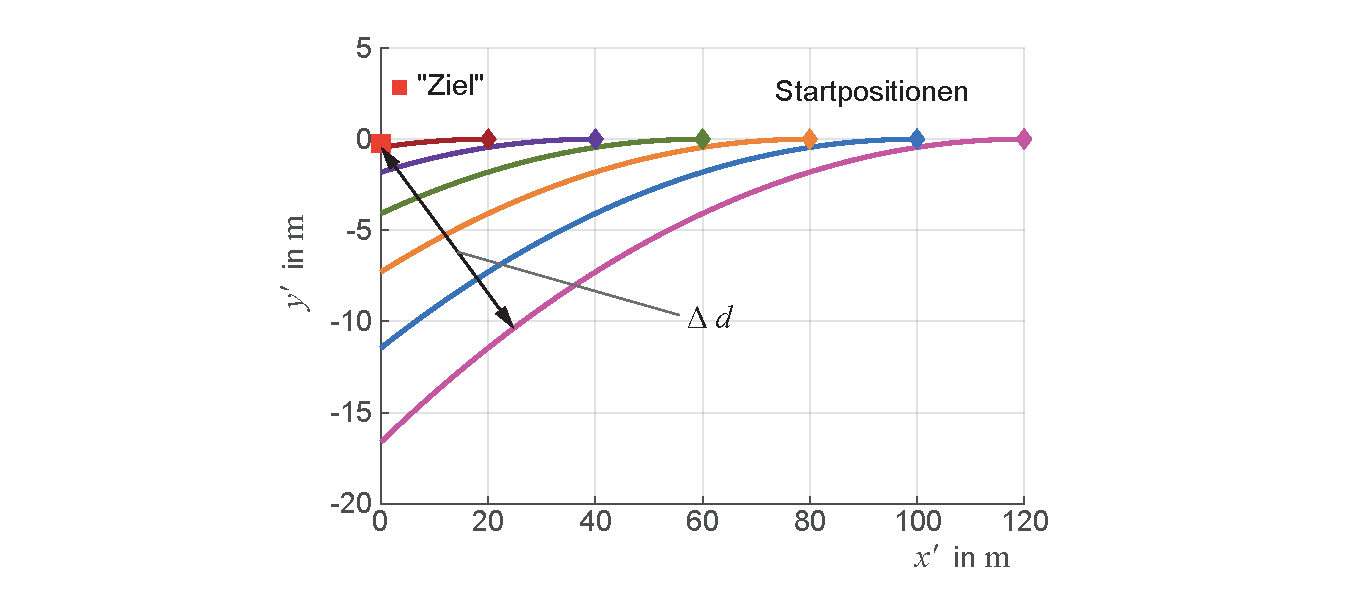
\includegraphics[width=\textwidth]{DirektAnflugISS.pdf} 
	\caption[Trajektorien eines Raumtransporters bei Anflug.]{Trajektorien eines Raumtransporters f�r verschiedene Anfangspunkte des Rendezvous-Man�vers (Anflug unter Schub in direkter Sichtlinie). Eingezeichnet ist auch der erreichte Endabstand $\Delta d$ (des jeweiligen Anflugs von $x_0'$) vom Zentrum der Docking-Vorrichtung f�r eine Anfangsgeschwindigkeit von $v_0 =  \SI{1}{\metre\per\second}$. (Nach \cite{Carroll2019}, siehe \probref{adyn_rendezvous01} \bzw \mscr~\mladynref{Rendezvous04.m})} \label{abb:adyn_rendezvous04a}
\end{figure}

\subsection{Wiederankopplung LM und CSM von Apollo 11}\label{kap:adyn_rendezvous_apollo11}

Ein besonders interessanter und zugleich f�r die erste bemannte Mondlandung extrem erfolgskritischer Fall eines Weltraum-Rendezvous war die Wiederankopplung der Mondf�hre von Apollo 11 (\gls{LM}\index{LM} "`The Eagle"', kurz: LM) nach der erfolgreichen Mondlandung mit den Astronauten Armstrong\footnote{Neil Alden Armstrong (1930--2012) war ein US-amerikanischer Testpilot und Astronaut. Er war Kommandant von Apollo 11 und betrat am 21. Juli 1969 als erster Mensch den Mond.}\indexp{Armstrong, Neil Alden} und Aldrin\footnote{Buzz Aldrin (geb. 1930)\indexp{Aldrin, Buzz} ist ein ehemaliger US-amerikanischer Astronaut, der im Rahmen der Apollo-11-Mission kurz nach Neil Armstrong als zweiter Mensch den Mond betrat.} an das Mutterschiff (\gls{CSM}\index{CSM}, kurz: CSM) mit dem Piloten Collins\footnote{Michael Collins (1930--2021) war ein US-amerikanischer Astronaut und umkreiste als Pilot des CSM einsam den Mond, w�hrend Armstrong und Aldrin die Mondoberfl�che betraten.}\indexp{Collins, Michael}. Details dieses Flugabschnitts sind in dem sehr lesenswerten Apollo Flight Journal \cite{Apollo11FJ} beschrieben.\\
Wir wollen den finalen Flugabschnitt des LM zwischen dem Zeitpunkt der \gls{TPI}\index{TPI} (TPI-Burn) und dem Bremsman�ver \gls{TPF}\index{TPF} (TPF) modellieren, vgl.~\figref{adyn_rendezvous05}.\footnote{Die vorhergehenden Flugabschnitte kann der Leser leicht mit dem Wissen aus dem \kap{adyn_maneuvers} nachvollziehen.}
Zum Zeitpunkt des TPI war das LM auf einer \ca 28 km tieferen Bahn als das CSM, \dh $y_0'=y_\text{LM}'\approx -\SI{28}{\kilo\metre}$. Der direkte Abstand zwischen LM und CSM betrug zu diesem Zeitpunkt \ca $\SI{56}{\kilo\metre}$, womit das CSM unter einem H�henwinkel von $\theta_0 = 26.5\degree$ vom LM aus "`gesehen"' wurde.\\

\begin{figure}[H]
	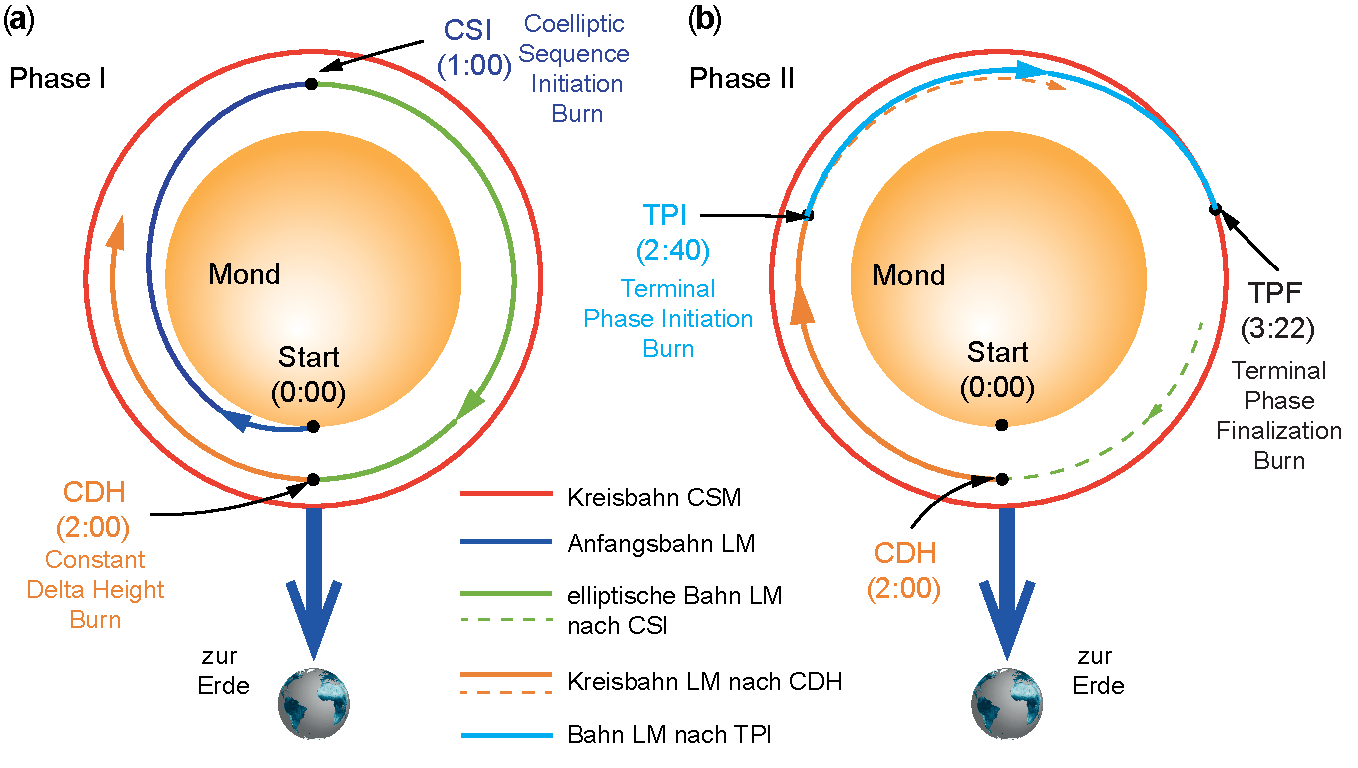
\includegraphics[width=\textwidth]{Apollo11LMCSMRendezvous.pdf} 
	\caption[Rendezvous von CSM und LM von Apollo 11.]{Rendezvous von CSM und LM von Apollo 11. \fa Phase I: Der Flug zum CSM begann mit dem Start des LM von der Mondoberfl�che und den Transfer in eine elliptische Bahn von $\SI{87.6}{} \,\mathrm{x}\, \SI{17.6}{\kilo\metre}$. %(\bzw  47.3 x 9.5 Nautische Meilen (die Ma�einheit der NASA)) 
	Nach einer Stunde hat das LM den apolunaren Punkt erreicht und kommt durch einen sogenannten CSI-Burn (\gls{CSI}) auf eine kreisf�rmigere Bahn von $\SI{92.5}{} \,\mathrm{x}\, \SI{85.0}{\kilo\metre}$. %(\bzw  50 x 46 Nautische Meilen)
	Durch einen weiteren Burn (CDH) erreicht das LM eine Bahn mit konstanter H�he und ist damit in einem konstanten H�henabstand von \ca $\SI{28}{\kilo\metre}$ zum CSM.
	%(\bzw  15 Nautischen Meilen)
  \fb Nach weiteren 40 Minuten erfolgt der so genannte TPI-Burn (\gls{TPI}), welche das LM auf die finale Rendezvous-Bahn bringt. 
%Nach diesem Burn fliegt das LM in einer nahezu geraden Linie in Bezug auf das feste KOS\ der Sterne auf das CSM zu. Tats�chlich haben die Astronauten die Fixsterne als visuelle Referenz zur Korrektur der Ann�herung benutzen k�nnen, da sich das LM auf der Nachtseite des Mondes befand. Die finale Phase der Ann�herung und das Bremsman�ver (TPF) erfolgten dann bei Tageslicht. %Zwischen TPI und TPF gab es zwei weitere kleinere Kurskorrekturen, die wir hier aber nicht weiter ber�cksichtigen m�ssen.
	(Nicht ma�st�bliche Zeichnung nach dem NASA Flight Journal von Apollo 11.)}
	\label{abb:adyn_rendezvous05}
\end{figure}

Wir haben in \kap{adyn_rendezvous} gelernt, dass f�r einen Burn zum direkten Anflug ein anderer Zielwinkel $\gamma$ angenommen werden muss als der direkte Sichtwinkel $\varphi_0 =\arctan({y_0'/x_0'})$. Um diesen Winkel $\gamma$ mit den CW-Gleichungen \eqref{eq:adyn_rendez27} zu berechnen, brauchen wir die Anfangsgeschwindigkeit $\vec{v}_{\text{LM},0}$ des LM im CSM-\KOS\ vor dem Burn. Wir haben diese bereits im vorhergehenden \kap{adyn_rendezvous_ISS} hergeleitet. Wir benutzen das Ergebnis hier, jetzt aber f�r zwei kreisf�rmige Bahnen (f�r CSM und LM). Dann folgt aus Gleichung \eqref{eq:adyn_rendez34} eine Geschwindigkeit des LM vor dem Burn zu:
\begin{align}
	\vec{v}_{\text{LM},0} = \lk \omega_\text{LM} - \omega_\text{CSM} \rk \, \lek \lk R_\text{CSM} + y_0' \rk \, \vecpeX - x_0 \, \vecpeY \rek \,. \label{eq:adyn_rendez43}
\end{align}
Die $x_0',\, y_0'$ ergeben sich aus einfacher geometrischer Betrachtung aus \figref{adyn_rendezvousKOS02} und die Kreisfrequenzen der Umlaufbahnen sind gegeben durch:
\begin{subequations}
	\begin{align}
		\omega_\text{CSM} &= \sqrt{\frac{G\,m_\text{M}}{R_\text{CSM}{}^3}} \approx \SI{8.8e-4}{\radian\per\second} \,,\\
		\omega_\text{LM} &= \sqrt{\frac{G\,m_\text{M}}{R_\text{LM}{}^3}} = \sqrt{\frac{G\,m_\text{M}}{\lk R_\text{CSM} - \Delta h\rk^3}} \approx \SI{9.0e-4}{\radian\per\second}\,, \label{eq:adyn_rendez44}
	\end{align} 
\end{subequations}
worin $m_\text{M}$ die Masse des Mondes und $R_\text{CSM},\, R_\text{LM}$ die Bahnradien der beiden Raumschiffe vor dem TPI sind. Wir k�nnen Gleichung \eqref{eq:adyn_rendez43} f�r $x_0',\, y_0' \ll R_0$ entwickeln, indem wir f�r $\omega_\text{LM}$ n�herungsweise $\omega_\text{LM} \approx \sqrt{\lk G\,m_\text{M}\rk/\lk R_\text{CSM} - y_0'\rk^3} $ schreiben und erhalten dann aus \eqref{eq:adyn_rendez43}
\begin{align}
	\vec{v}_{\text{LM},0} = \begin{pmatrix} v_{\text{LM},0,x'} \\ v_{\text{LM},0,y'} \end{pmatrix}
	= -\frac{3}{2}\,\omega_\text{CSM} \, y_0' \,\begin{pmatrix} -x_0'/R_0 \\ 1 + y_0'/R_0 \end{pmatrix} \begin{pmatrix} \vecpeX \\ \vecpeY \end{pmatrix}\,.
	\label{eq:adyn_rendez46}
\end{align}
Damit haben wir alle Gr��en, um aus den CW-Gleichungen den Geschwindigkeitsbedarf f�r das TPI-Man�ver, die Richtung des TPI-Burn und die finale Trajektorie nach dem TPI zu berechnen.
Das Ergebnis der Rechnungen haben wir f�r verschiedene $y_0'$ in \figref{adyn_rendezvous06} dargestellt. Man berechnet f�r den Geschwindigkeitsbedarf des TPI-Burn 
\begin{align}
	\Delta v = \sqrt{\lk \dot{x}_0' - v_{\text{LM},0,x'}\rk^2 + \lk \dot{y}_0'-v_{\text{LM},0,y'}\rk^2}\,,\label{eq:adyn_rendez47}
\end{align}
wobei sich die $\dot{x}_0',\,\dot{y}_0'$ aus \eqref{eq:adyn_rendez24} berechnen. F�r die drei F�lle aus \figref{adyn_rendezvous06} ergeben sich Geschwindigkeitsbedarfe von $\Delta v = 8.0 \ldots \SI{6.9}{\metre\per\second}$ und ein Zielwinkel des Burn von $\gamma= 19.8\degree$ (nicht zu verwechseln mit dem Abflugwinkel $\alpha$), was gut mit der NASA Planung von $\Delta v = \SI{7.5}{\metre\per\second}$ �bereinstimmt. Man erkennt auch aus \figref{adyn_rendezvous06}, dass selbst bei Verpassen des optimalen Zeitpunktes des TPI-Burn (\dh der richtigen H�he $y_0'$) die Burn-Richtung und auch die Gr��e von $\Delta v$ relativ unkritisch sind f�r den Erfolg des Man�vers, was sicher etwas vom Stress der Astronauten wegnahm.
\begin{figure}[H]
	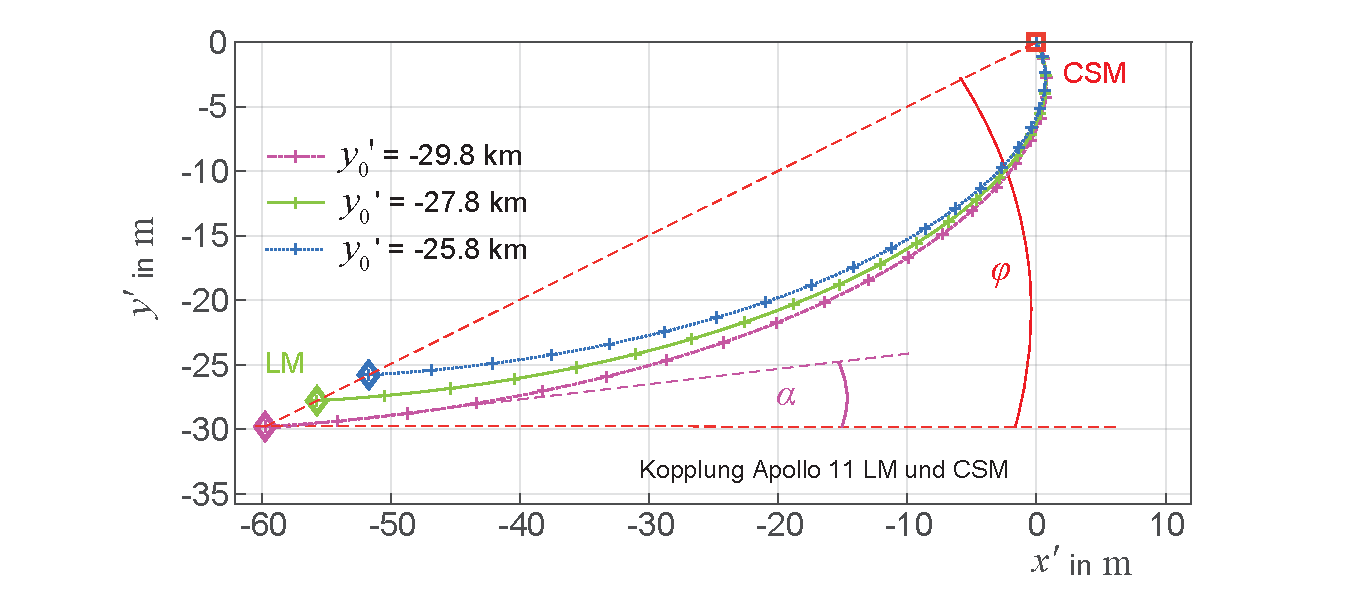
\includegraphics[width=\textwidth]{Apollo11LMCSMTrajektorie.pdf} 
	\caption[Trajektorien des LM im Anflug auf das CSM von Apollo 11.]{Trajektorien des LM im Anflug auf das CSM von Apollo 11 f�r verschiedene H�hen des TPI-Burn. Siehe \probref{adyn_rendezvous02} \bzw \mscr~\mladynref{LMCSMApollo11.m}.}
	\label{abb:adyn_rendezvous06}
\end{figure}
Wir m�chten noch erw�hnen, dass nach der erfolgreichen Kopplung und dem Umstieg der Astronauten vom LM ins CSM das LM wieder abgesprengt wurde. Das wohl mit bedeutsamste Fahrzeug der Menschheitsgeschichte war damit sich selbst \bzw dem Gravitationsfeld des Mondes �berlassen. Bis heute konnte man keinen Einschlagkrater des LM auf dem Mond finden, so dass man davon ausgehen muss, dass der \textit{"`Eagle"'}  noch immer den Mond umkreist. Wer sich Modellrechnungen f�r eine m�gliche Bahn des LM anschauen will, dem seien die Referenzen \cite{Khan2021} und \cite{meador2021} empfohlen. Letztere eignet sich auch f�r einen Einstieg in das von der NASA der Allgemeinheit zur Verf�gung gestellte GMAT-Paket \url{software.nasa.gov/software/GSC-17177-1}, in welchem auch sehr leistungsf�hige \matlab-Programme f�r die Astrodynamik und Himmelsmechanik zu finden sind.




 
\clearpage
\section{Start aus der Erdatmosph�re und Wiedereintritt}\label{kap:adyn_launch_reentry}

\subsection{Kr�fte im erdnahen Weltall}\label{kap:adyn_forces}

Zum Abschluss der Astrodynamik wollen wir uns mit Situationen besch�ftigen, in denen neben der Gravitationskraft weitere Kr�fte eine Rolle spielen. Das ist insbesondere bei Starts von der Erdoberfl�che, Bahnen in niedriger H�he und nat�rlich beim Wiedereintritt in die Erdatmosph�re der Fall. \\
In den meisten F�llen wird man die Bewegungsgleichung nur numerisch integrieren k�nnen, wir wollen aber in einigen F�llen auch N�herungsformeln angeben. \\
Zun�chst untersuchen wir die zur Gravitation der Erde (die als Zentralkraft angenommen wird) zus�tzlich auftretenden Kr�fte, um dann die jeweiligen relevanten Kr�fte bei der Berechnung von Start, Wiedereintritt in die Erdatmosph�re \bzw in Flug in niedrigen Orbits zu ber�cksichtigen. 

\subsubsection{Atmosph�rische Reibung \index{Drag}\index{Reibung!atmosph�rische}}\label{kap:adyn_drag}

Die atmosph�rische Reibung stellt die gr��te nicht-gravitative St�rung f�r Satelliten und Raumsonden bei Start und Wiedereintritt sowie Fl�gen in extrem geringen Flugh�hen dar. Die genaue Modellierung der atmosph�rischen Reibung ist aber nicht ganz einfach, da \ia die Eigenschaften der Atmosph�re in den verschiedenen H�henbereichen nicht ausreichend genau bekannt sind und auch die genaue Wechselwirkung der atmosph�rischen Teilchen mit der Form und Oberfl�che des Raumschiffs stark variiert. \\
Wir werden deshalb auf das uns aus Band I bereits bekannte einfache Kraftmodell der Newtonschen Reibung zur�ckgreifen. 
Nach diesem beschreiben wir die atmosph�rische Reibung (Englisch \textit{\gls{drag}}\index{Drag|textbf}) mit:
\begin{align}
    \vec{F}_\text{D} = -\frac{1}{2}\,c_\text{D}\,A\,\varrho\,v_\text{R}{}\,\dot{\vec{r}}\,. \label{eq:adyn_forces01}
\end{align}
Hierin ist $c_\text{D}$ der atmosph�rische Reibungskoeffizient, der typischerweise im Bereich von $\SI{1.5}{}\ldots\SI{3.0}{}$ liegt, $A$ die effektive Querschnittsfl�che des Raumschiffs, $\varrho$ die (h�henabh�ngige) Dichte der Atmosph�re und $v_\text{R}$ der Betrag des momentanen Geschwindigkeitsvektors~$\dot{\vec{r}}$. F�r die Dichte werden in der Astrodynamik verschiedene Modelle verwendet, im einfachsten Fall kann $\varrho$ nach der barometrischen H�henformel \index{H�henformel!barometrische|textbf} mit 
\begin{align}
    \varrho = \varrho_0\,\e^{-\frac{h}{H_0}} \label{eq:adyn_barom_h_fomulae}
\end{align}
angegeben werden,
worin $H_0$ und $\varrho_0$ f�r die Standardatmosph�re \cite{ISA1976} durch
\begin{align}
    H_0= \frac{R\,T}{\tilde{M}_\text{L}\,g} = \SI{6.7}{\km}~~~\text{und}~~~\varrho_0 = \SI{1.752}{\kg\per\metre\cubed} \label{eq:adyn_barom_h_fomulae_zusatz}
\end{align}
gegeben sind. 
$R$ ist die universelle Gaskonstante $R= \SI{8.314}{\joule\per\K\per\mole}$, $T$ die gegebenenfalls h�henabh�ngige absolute Temperatur und $\tilde{M}_\text{L}$ ist die (mittlere) molare Masse der Luft $\tilde{M}_\text{L}=\SI{28.9e-3}{\kg\per\mole}$. Letztlich wird die Dichte noch von Faktoren wie der Einstrahlung der Sonne (die eine halbt�gliche Variation der Dichte bewirkt) und auch geomagnetischen Einfl�ssen abh�ngen, die Teilchendichte und -zusammensetzung beeinflussen.\footnote{Ein in der Astrodynamik weit verbreitetes Modell ist das Harris-Priester-Modell, das aber �ber den Umfang und Anspruch dieses Buches hinausgeht. Wir verweisen auf die weiterf�hrende Literatur \cite{Walter2018, Montenbruck2012}.} 
Wir werden f�r unsere grobe Absch�tzung \ia mit der barometrischen H�henformel oder der tabellierten Standardatmosph�re (US Standard Atmosphere Table \cite{ISA1976}) arbeiten, was f�r unsere Zwecke meist ausreichend ist.
Es sei noch darauf hingewiesen, dass die Atmosph�re neben dem Drag auch noch einen Auftrieb bewirken kann, den wir beim Wiedereintritt zu ber�cksichtigen haben, sonst aber vernachl�ssigen werden. 

\subsubsection{Strahlungsdruck \index{Strahlungsdruck}} \label{kap:adyn_strahlungsdruck}

Der Strahlungsdruck ist eine weitere St�rkraft. Sie wird hervorgerufen durch den Druck, den ein Strahl von Photonen auf einen K�rper aus�bt, wenn dieser auf die Oberfl�che des K�rpers trifft. Wir werden diese in der Elektrodynamik herleiten, hier geben wir nur die f�r die Astrodynamik relevante Beziehung an:
\begin{align}
    F_\text{Rad} = \frac{s_0}{c}\,\lk\frac{\au}{d}\rk^2 \label{eq:adyn_forces04}
\end{align}
mit $s_0 = \hat{s}_0\,\lek 1+0.034\,\cos\lk\frac{360\,n}{365.25}\rk\rek$ und $\hat{s}_0 = \SI{1376.6}{\W\per\square\metre}$ (Solarkonstante). Dabei sind $n$ die Nummer des Tages eines Jahres, $d$ der Abstand der Raumsonde zur Sonne und $\au$ wie �blich die astronomische Einheit.\\
Die tats�chlich auf ein Raumschiff ausge�bte Kraft des Strahlungsdrucks h�ngt von weiteren Faktoren ab, \zb der tats�chlichen Geometrie des Raumschiffs, der  Abschattung der Sonne durch andere Himmelsk�rper \ua Wir werden den Strahlungsdruck im weiteren nicht ber�cksichtigen, er ist bei Start und Wiedereintritt \ia gegen den Drag zu vernachl�ssigen, muss aber bei HEO-Satelliten und im interplanetaren Raumflug\footnote{Der Strahlungsdruck kann besonders im interplanetaren Raum auch zum Antrieb benutzt werden. Dazu werden Raumschiffe mit sogenannte Sonnensegeln, die die Solarstrahlung zum Antrieb des Raumschiffs nutzen, ausgestattet. In \cite{Bailer2021} wird die japanische Mission IKAROS behandelt, die mit einem solchen Antrieb im interplanetaren Raum unterwegs ist.} unbedingt ber�cksichtigt werden. 

\subsubsection{Gravitative St�rungen} \label{kap:adyn_gravity_pertubations}
Neben Drag und Strahlungsdruck gibt es auch St�rungen, die durch das nicht vollst�ndig sph�rische Gravitationsfeld hervorgerufen werden. Solchen St�rungen werden durch die Abweichung der Form der Erde von einer idealen Kugel oder vom Gravitationseinfluss anderer Planeten und Monde hervorgerufen. Wir sind diesen Kr�ften bereits mehrfach begegnet. Im Kapitel 1.5.6 in Band I hatten wir bei der Behandlung der Pr�zession der Erde und in diesem Band im \kap{Periheldrehung} bei der Perihelverschiebung des Merkurs bereits solche St�rungen ber�cksichtigt. \\
Die allgemeine Vorgehensweise zur Berechnung solcher St�rungen mit Hilfe der Potential\-theorie hatten wir ausf�hrlich bei der Theorie der Gezeiten in \kap{hm_gezeiten_Laplace} behandelt. Wir haben das reale, von der sph�rischen Symmetrie abweichende Gravitationspotential $U\lk \vec{r} \rk  = U(r,\, \phi,\,\lambda)$ nach \eqref{eq:hm_pot_theo07a} durch eine Entwicklung nach Kugelfl�chenfunktionen\index{Kugelfl�chenfunktionen} des Winkels der geozentrischen Breite $\phi$ beschrieben. Der Einfachheit halber haben wir Rotationssymmetrie angenommen (also keine Abh�ngigkeit von der L�nge $\lambda$) und brauchen deshalb nur die Entwicklung nach $\phi$ zu betrachten. In \eqref{eq:hm_pot_theo07a} hatten wir den Winkel~$\theta$ verwendet und deshalb bei den Legendre-Polynomen\index{Legendre-Polynome} $\PL n(\,\cos\theta)$ geschrieben.  Hier aber benutzen wir die geozentrische Breite $\phi=\frac{\pi}{2}-\theta$ , so dass sich ergibt: 
\begin{align}
    \frac{1}{m}\,U\lk r,\phi\rk =-\frac{M\,G}{r}\,\lk 1-\sum\limits_{n-2}^\infty\,J_n\,\lk\frac{R_0}{r}\rk^n\,\PL n\,\lk\sin\phi\rk\rk \,.\label{eq:adyn_forces05} 
\end{align}
Die St�rterme $J_n$ in \eqref{eq:adyn_forces05} bestimmen sich aus der Form und Masseverteilung der Planeten und werden oft auch als zonale Harmonische\index{Harmonische!zonale} bezeichnet. Nehmen wir die f�r die meisten Himmelsk�rper g�ltige N�herung eines oblaten Rotationsellipsoids an, gilt:
\begin{align*}
    J_2 \gg J_n ~~~~ \forall\, n>2\,.
\end{align*}
F�r die Erde gilt beispielsweise $ |J_2| = \SI{1.08e-3}{} \: \gg \:|J_4| = \SI{1.62e-6}{}$, 
so dass es f�r unsere Zwecke gen�gt, nur $J_2$ bei der Berechnung von \eqref{eq:adyn_forces05} zu ber�cksichtigen. 
Bei der Behandlung der Gezeiten in \kap{hm_gezeiten} hatten wir auch gesehen, dass das Potential der Gezeitenkr�fte eine �hnliche mathematische Struktur aufweist, wie das Potential welches durch einen Rotationsellipsoiden erzeugt wird. Wir k�nnen daher annehmen, dass die Gezeitenkr�fte von Sonne und Mond �hnliche St�rwirkungen auf einen Erdorbit eines Satelliten hervorrufen, wie die St�rungen, die von der abgeplatteten Form der Erde herr�hren. \\
Tabelle \ref{tab:adyn_forces01} zeigt die relativen Gr��enverh�ltnisse der einzelnen St�rungen f�r eine Bahn $h=\SI{400}{\km}$ (ISS) und eine Bahn $h\approx\SI{40000}{\km}$ (GEO-Satellit).\\
Die Frage ist nun, wie die einzelnen St�rbeschleunigungen wirken. Da der Drag immer entgegen der Bewegungsrichtung wirkt, f�hrt er zu einer Geschwindigkeits�nderung und somit auch einer �nderung von Halbachse und Elliptizit�t der Bahn. Die zonalen Harmonischen $J_n$ und auch die Gravitationseinfl�sse von Sonne und Mond bewirken eine Drehung der Apsidenlinie \bzw Perig�umsverschiebung (\vgl \kap{Periheldrehung}) und eine Verschiebung des Knotens der Bahn. Abh�ngig von der Einstrahlcharakteristik der solaren Strahlung kann der Strahlungsdruck sowohl eine �nderung des Bahnradius als auch der Apsidenlinie bewirken.\\

\begin{table}[ht]
    \begin{center}
    \begin{tabular}{|C{4cm}|C{3cm}|C{3.0cm}|}
    \hline
    \rule{0pt}{3pt}& &  \\
      $\text{St�rung durch}$ & ISS/LEO-Satellit  & GEO-Satellit \\
    %\rule{0pt}{3pt}& &  \\
       & $h\approx\SI{500}{\km}$ & $h\approx\SI{40000}{\km}$ \\
    \rule{0pt}{3pt}& &  \\
    \hline
    %\rule{0pt}{3pt}& &   \\
    \rule{0pt}{6pt} Abplattung Erde $J_2$&$\SI{e-5}{}$ & $\SI{e-8}{}$ \vphantom{$I^{I^I}$} \\
    %\rule{0pt}{3pt}& &  \\
    \rule{0pt}{6pt} $\text{Gravitation Mond}$ &$\SI{e-9}{}$ & $\SI{5e-9}{}$ \\
    %\rule{0pt}{3pt}& &  \\
    \rule{0pt}{6pt} $\text{Gravitation Sonne}$ &$\SI{5e-10}{}$ & $\SI{2e-9}{}$ \\
    %\rule{0pt}{3pt}& &  \\
    \rule{0pt}{6pt} Abplattung Erde $J_4$&$\SI{e-8}{}$ & $\SI{1e-11}{}$ \\
    %\rule{0pt}{3pt}& &  \\
    \rule{0pt}{6pt} $\text{Strahlungsdruck}$ &$\SI{5e-8}{}$ & $\SI{5e-8}{}$ \\
    %\rule{0pt}{3pt}& &  \\
    \rule{0pt}{6pt} $\text{Drag}$ &$\SI{6e-8}{}$ & $\approx 0$ \\
    %\rule{0pt}{3pt}& &  \\
    \hline
    \end{tabular}    
    \end{center}
    \caption{Ungef�hre Gr��enordnungen von St�rbeschleunigungen (alle in $\SI{}{\km\per\square\second}$) auf Satelliten in verschiedenen H�hen �ber der Erde \cite{Montenbruck2012, Walter2018}.}
    \label{tab:adyn_forces01}
\end{table}
\subsection{Raketenstart von der Erde}\label{kap:adyn_launch}

Ein Raketenflug in eine erdnahe Umlaufbahn kann in drei Phasen unterteilt werden:
\begin{itemize}
	\item Start und die Schubphase, in der die Rakete mit dem Raumschiff auf eine Geschwindigkeit~$v_\text{f}$ bis zum �bergangspunkt (\gls{Brennschluss}) beschleunigt wird,
	\item die Bewegung auf einer freien Kepler-Trajektorie bis zum Erreichen des Apog�ums,
	\item den Burn mit $\Delta v$, der das Raumschiff auf die gew�nschte Zielumlaufbahn bringt.
\end{itemize}
Diese Phasen sind in \figref{adyn_launch01}a dargestellt. Wir weisen bereits hier darauf hin, dass man sich das Problem der R�ckkehr eines Raumschiffs zur Erde, insbesondere unter Ber�cksichtigung der Phase des Wiedereintritts in die Erdatmosph�re, als genau umgekehrt ablaufende Dynamik vorstellen kann (\figref{adyn_launch01}b). Wir werden das im \kap{adyn_reentry} genauer betrachten.

\begin{figure}[H]
\includegraphics[width=\textwidth]{PhasenStartvonErde.pdf}
\caption[Phasen eines Raketenflugs vom Start bis in eine Erdumlaufbahn.]{\fa Phasen eines Raketenflugs vom Start auf der Erdoberfl�che in eine Erdumlaufbahn. Der �bergangspunkt ist hier durch das Ende der Schubphase definiert. \fb Phasen eines Raketenflugs aus einem Erdorbit bis zur Landung auf der Erdoberfl�che. Der �bergangspunkt  ist hier durch den Eintritt in den sogenannten aerodynamischen Bereich (\kap{adyn_reentry}) definiert.}
\label{abb:adyn_launch01}
\end{figure}

In \figref{adyn_launch02} sind:
\begin{center}
\begin{tabular}{L{2cm}L{10cm}}
        \rule{0pt}{12pt}$\vec{F}_\text{S}, \vec{F}_\text{D}$, $\vec{F}_\text{A}$ & die Schubkraft, der \index{Drag}\textit{\glslink{drag}{Drag}} \bzw der Auftrieb,  \\
        \rule{0pt}{12pt}$\alpha$ & der Winkel zwischen Schub $\vec{F}_\text{S}$ und der Geschwindigkeit der Rakete $\vec{v}$, im Englischen \index{Angle of Attack}\textit{\glslink{AngleOfAttack}{Angle of Attack (AoA)}} genannt, \\
        \rule{0pt}{12pt}$\gamma$ & der Winkel zwischen der Geschwindigkeit $\vec{v}$ und dem lokalen Horizont, im Englischen \index{Flight Path Angle}\textit{\glslink{FlightPathAngle}{Flight Path Angle (FPA)}} $\gamma$ genannt,\\
         \rule{0pt}{12pt}$h, s$ & die H�he �ber der Erdoberfl�che \bzw  der zur�ckgelegte Weg der Sonde.\\
\end{tabular}
\end{center}

Wir berechnen nun unter Ber�cksichtigung der �u�eren Kr�fte die Aufstiegsbahn einer Rakete. Nach Tabelle \ref{tab:adyn_forces01} m�ssen wir f�r die Aufstiegsphase sicher den Drag einrechnen, alle anderen Kr�fte k�nnen wir im Bereich $R_\text{E} < r < R_\text{E} + h$ mit $h \leq \SI{100 }{\km}$ vernachl�ssigen. \\
Um die Bewegungsgleichungen aufzustellen, betrachten wir \figref{adyn_launch02}a. In vektorieller Form lauten diese im Erd-\KOS :
\begin{align}
      m_\text{R}(t)\,\ddot{\vec{r}} &= \vec{F}_\text{S} (t) + m_\text{R}(t)\,\vec{g}(\vec{r}) + \vec{F}_\text{D}(\dot{\vec{r}}, \vec{r}) + \vec{F}_\text{A}(\dot{\vec{r}}, \vec{r})  \,. \label{eq:adyn_launch_vec}
\end{align}

\begin{figure}[H]
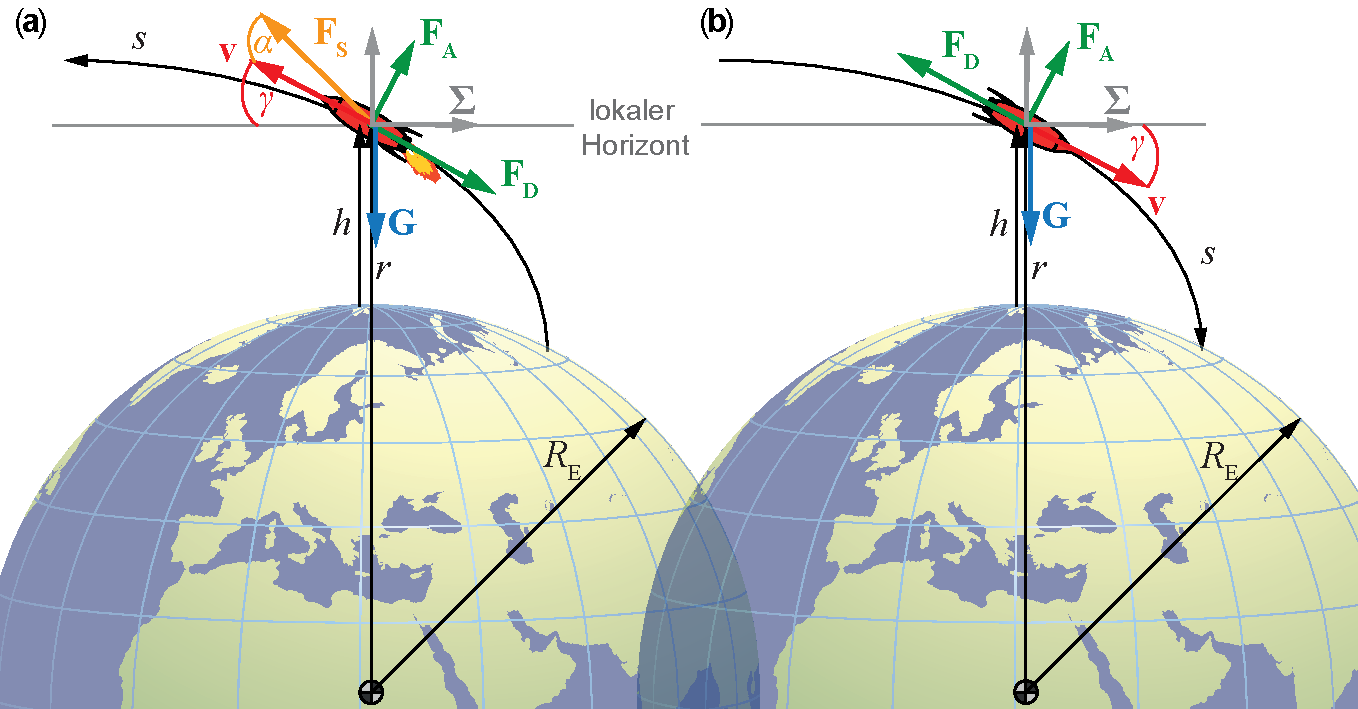
\includegraphics[width=\textwidth]{RaumflugstartErde.pdf}
\caption[Kr�fte beim Raketenstart von der Erdoberfl�che und beim Wiedereintritt.]{Zur Herleitung der Bewegungsgleichungen f�r den Raketenstart \bzw den Wiedereintritt in die Erdatmosph�re. \fa Kr�fte beim Raketenstart von der Erdoberfl�che. \fb Kr�fte beim Wiedereintritt in die Erdatmosph�re.}
\label{abb:adyn_launch02}
\end{figure}

Bei der Planung von realen Raumfahrtmissionen wird man \ia mit bekannten \bzw vorgegebenen  Gr��en $\vec{F}_\text{S}(t),\, \vec{F}_\text{D}(\dot{\vec{r}}, \vec{r})$ und $\vec{F}_\text{A}(\dot{\vec{r}}, \vec{r})$ die gesuchten Gr��en $\vec{r}$ und $\vec{v}=\dot{\vec{r}}$ aus \eqref{eq:adyn_launch_vec} numerisch berechnen. 

Wir werden nun ein System von skalaren Bewegungsgleichungen zur mathematischen Behandlung der Aufstiegsphase aus \eqref{eq:adyn_launch_vec} herleiten. 
Der Aufstiegsbereich wird als relativ klein angenommen, so dass $r, R_\text{E} \gg s,h$ und $R_\text{E}/r \approx 1$.
Ferner sollen die Kr�fte $\vec{F}_\text{D}(\dot{\vec{r}},\vec{r}), \vec{F}_\text{A}(\dot{\vec{r}},\vec{r})$ in der Bahn\-ebene des Raumschiffs liegen. Das erlaubt uns ein Behandlung als zweidimensionales Problem. Wir gehen weiter in ein mit dem Raumschiff mitbewegtes \KOS\ �ber, dessen $x$-Achsenrichtung mit dem lokalen Horizont zusammenf�llt (\figref{adyn_launch02}a). In diesem \KOS\ ergibt sich folgendes System von Bewegungsgleichungen\footnote{Auch hier sei wieder angemerkt, dass das Problem des Wiedereintritts in die Erdatmosph�re als genau umgekehrt ablaufende Dynamik gesehen werden kann, lediglich der Schub wird \ia Null sein. In \figref{adyn_launch02}b sind die wirkenden Kr�fte f�r diesen Fall dargestellt und im \kap{adyn_reentry} werden wir auf die nachfolgenden Rechnungen in diesem Kapitel Bezug nehmen.} f�r die vier unabh�ngigen\footnote{In einem zweidimensionalen System gibt es eigentlich nur zwei unabh�ngige Variablen, f�r die ein Differentialgleichungssystem 2. Ordnung nach der Zeit gilt. Dieses ist aber einem Differentialgleichungssystem 1. Ordnung nach der Zeit f�r vier unabh�ngigen Variablen �quivalent.} Variablen $v$, $\gamma$, $h$, $x$ (\probref{adyn_launch01a}): 

\begin{subequations}
    \begin{align}
        \frac{\D v}{\D t} &= \frac{F_\text{S}(t)\,\cos\alpha-F_\text{D}(h,v)}{m_\text{R}} -g(h)\,\sin\gamma\,,\label{eq:adyn_launch01a} \\
        v\,\frac{\D \gamma}{\D t}&= \frac{F_\text{S}(t)\,\sin\alpha + F_\text{A}(h,v)}{m_\text{R}} - \lk g(h) -\frac{v^2}{R_\text{E} + h}\rk \,\cos\gamma\,, \label{eq:adyn_launch01b}\\
        \frac{\D r}{\D t} &= \frac{\D h}{\D t} - v\,\sin\gamma\,~~\,~\rightarrow ~~ \frac{\D h}{\D t} \approx v\,\sin\gamma \,,\label{eq:adyn_launch01c} \\
        \frac{\D s}{\D t} &= \lk \frac{R_\text{E}}{r}\rk\,v\,\cos\gamma\,~~\rightarrow ~~ \frac{\D x}{\D t} \approx \,v\,\cos\gamma\,. \label{eq:adyn_launch01d}
    \end{align} \label{eq:adyn_launch01}
\end{subequations} 

Bekannte Parameter in \eqref{eq:adyn_launch01} sind $F_\text{S}\lk t\rk$, $F_\text{D}\lk h\rk$ und $g\lk h\rk$. Der FPA $\gamma$ ist aus folgendem Grund noch explizit zeitabh�ngig: Raketen starten aus Gr�nden der strukturellen Stabilit�t \iA senkrecht von der Erdoberfl�che ($\gamma_0 = 90\degree$). Nach einiger Zeit hat die Rakete eine H�he von $\SI{500}{}\ldots\SI{1000}{\metre}$ erreicht und es erfolgen dann eine oder mehrere sogenannte Nickkorrekturen\index{Nickkorrektur} des FPA um $\Delta \gamma\approx 1\degree\ldots8\degree$, die die Rakete in eine geneigte Bahn �bergehen lassen.\\
Die Bewegungsgleichung \eqref{eq:adyn_launch01a} kann formal integriert werden und ergibt dann mit der Raketen-Gleichung\index{Raketen-Gleichung} \eqref{eq:adyn_rocketequ} f�r $t=t_\text{f}$ (Zeit zum �bergangspunkt) eine Beziehung f�r den Betrag der Endgeschwindigkeit: 
\begin{align}
    v(t_\text{f}) &= \int\limits_0^t \frac{F_\text{S}}{m_\text{R}}\,\D t' - \underbrace{\int\limits_0^t \frac{F_\text{D}}{m_\text{R}}  \,\D t'}_{\mathrm{Reibungsverlust}} - \underbrace{\int\limits_0^t \frac{F_\text{S}\,(1-\cos\alpha)}{m_\text{R}}  \,\D t'}_{\mathrm{Steuerungsverlust}}  - \underbrace{\int\limits_0^t g\,\sin\gamma \,\D t'}_{\mathrm{Gravitationsverlust}} \nonumber \\
		&=  v_\text{G}\ln{\frac{m_0}{m_\text{f}}} - \Delta v_\text{D} - \Delta v_\text{S} - \Delta v_\text{G}  \,. \label{eq:adyn_launch07}
\end{align}
Hierin ist $v_\text{G}$ die in \kap{adyn_rockets} definierte Austrittsgeschwindigkeit der Treibgase der Rakete und $m_\text{f}$ ist �ber  $m_\text{f} = m(t_\text{f}) = m_0 - \dot{m}\,t_\text{f}$ gegeben. Diese Gleichung zeigt, dass zus�tzlich zum Antriebsbedarf nach der Raketen-Gleichung der Schub noch die Reibungs-, Steuerungs- und Gravitationsverluste kompensieren muss.\footnote{Die Steuerungsverluste durch einen AoA $\neq 0$ sind meist klein gegen die Reibungs- und Gravitationsverluste und k�nnen daher meist vernachl�ssigt werden. Den unterst�tzenden Effekt der Erdrotation betrachten wir am Ende dieses Kapitels.}\\
Wir wollen nun \eqref{eq:adyn_launch01} numerisch l�sen und werden uns die Rechnungen etwas vereinfachen, in dem wir den Auftrieb $F_\text{A}$ gleich Null setzen. Ebenso soll die Raketensteuerung so realisiert werden, dass $\vec{F}_\text{S}\parallel \vec{v}$, \dh $\alpha \approx 0$.  Ferner nehmen wir eine "`ebene"' Erde an, \dh $r, R_\text{E} \gg h$, $R_\text{E}/r \approx 1$ und $g \gg v^2/r$. Die Bewegungsgleichungen \eqref{eq:adyn_launch01} vereinfachen sich zu:
\begin{subequations}
    \begin{align}
        \dot{v} &= \frac{\D v}{\D t} = \frac{F_\text{S}\lk t\rk - F_\text{D}\lk h\rk}{m_\text{R}} - g\lk h\rk \,\sin\gamma\,,\label{eq:adyn_launch08a} \\
        \dot{\gamma}&= \frac{\D \gamma}{\D t} = \frac{g\lk h \rk}{v} \,\cos\gamma\,, \label{eq:adyn_launch08b} \\
        \dot{h} &= \frac{\D h}{\D t} = v\,\sin\gamma\,, \label{eq:adyn_launch08c} \\
        \dot{x} &= \frac{\D x}{\D t} = v\,\cos\gamma\,. \label{eq:adyn_launch08d}
    \end{align} \label{eq:adyn_launch08}
\end{subequations}

F�r den Drag $F_\text{D}\lk h\rk$ benutzen wir die Beziehung \eqref{eq:adyn_forces01} und die einfache barometrische H�henformel \eqref{eq:adyn_barom_h_fomulae}. 
Die numerische L�sung erfolgt mit der \matlab-Routine \odevf, wobei $F_\text{S}\lk t\rk$ f�r die verschiedenen Bahnphasen explizit zeitabh�ngig sein kann. Der FPA kann durch einzelne sogenannte Nickkorrekturen zu Zeiten $t=t_\text{Nick}$ in Spr�ngen ver�ndert werden. In \figref{adyn_launch03} ist das Ergebnis der Rechnungen, die im \mscr{} \mladynref{RaketenstartReal.m} hinterlegt sind, f�r verschiedene Parameters�tze der Nickkorrektur $\Delta \gamma$ gezeigt. Auch ein Vergleich zum Fall mit vernachl�ssigbarer aerodynamischer Reibung ist angegeben. Man erkennt sehr sch�n, welchen gro�en Einfluss die Nickkorrektur auf die Bahnh�he und Bahnform der Rakete hat. \\

Abschlie�end seien noch einige Bemerkungen zur Optimierung der Aufstiegsphase einer Raketenmission in einen erdnahen Orbit gegeben.
Offensichtlich geht es zum einen darum, den Gesamtantriebsbedarf $\Delta v$ so gering wie m�glich zu machen. Zum anderen soll auch eine vorgegebene Bahn unter bestimmten Randbedingungen (�bergangspunktfestlegung, Zeitprofil, Schub, Nickprofil etc.) erreicht werden. Die Optimierung geschieht folgenderma�en: Man l�st die Bewegungsgleichungen \eqref{eq:adyn_launch01} \bzw \eqref{eq:adyn_launch08} unter Ber�cksichtigung der gegebenen Funktionen $F_\text{S}(t),\, m_\text{R}(t)$ und $\Delta \gamma(t,h)$, der Anfangs- und Endbedingungen f�r $h, \gamma$ und $v$ und sucht das minimale $\Delta v$, in dem man die Summe der einzelnen Verlustbeitr�ge in \eqref{eq:adyn_launch07} minimiert. Daraus ergibt sich 
die finale Geschwindigkeit $v_\text{f}$ am �bergangspunkt in die freie Trajektorie zu:
\begin{align}
    v_\text{f} = v_\text{G}\ln{\frac{m_0}{m_\text{f}}} - \Delta v_\text{D} - \Delta v_\text{G} + \Delta v_\text{E} \,. \label{eq:adyn_launch09}
\end{align}
Hierin sind $\Delta v_\text{D}$ und $\Delta v_\text{G}$ die in \eqref{eq:adyn_launch07} definierten Antriebsbedarfe zur Kompensation der Reibung und der Arbeit im Gravitationsfeld.

\begin{figure}[H]
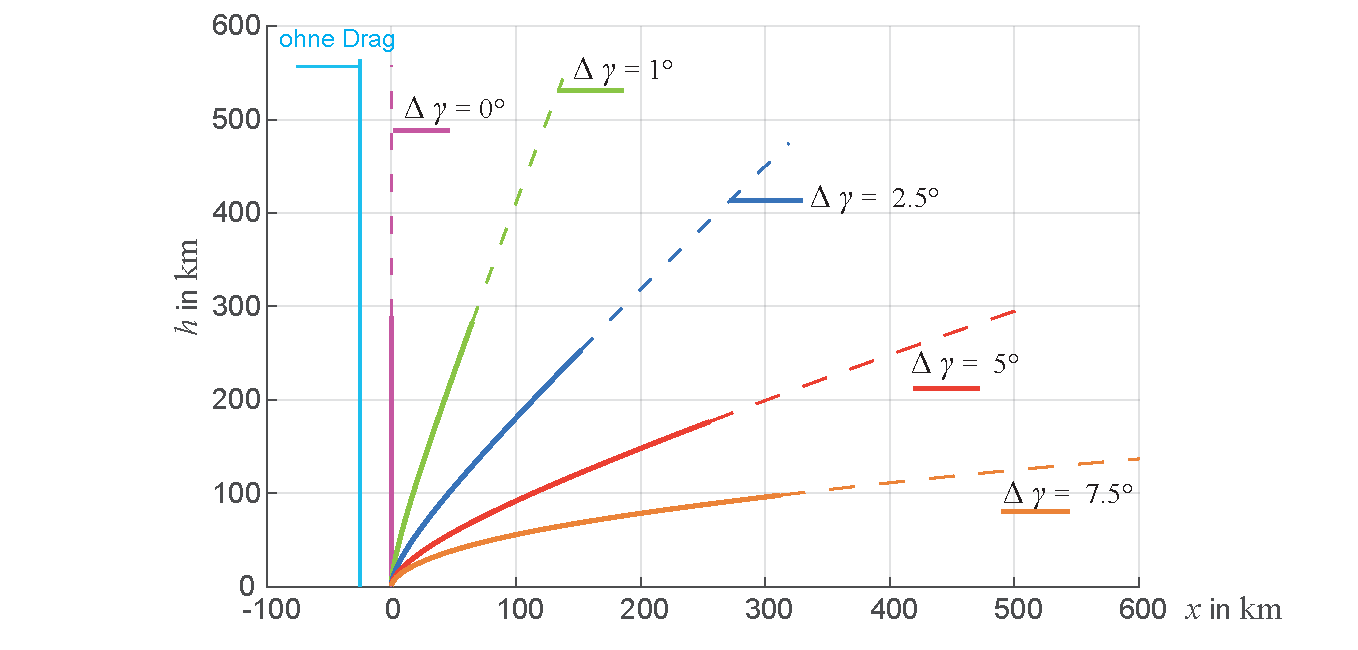
\includegraphics[width=\textwidth]{RaketenstartReal.pdf}
\caption[Trajektorie eines Raketenstarts von der Erdoberfl�che.]{Trajektorie eines Raketenstarts von der Erdoberfl�che f�r verschiedene Nickwinkel $\Delta \gamma$. Parameter: 
$c_\text{D}\,A = \SI{1.5}{\metre\squared}$ (Widerstandsbeiwert x Fl�che), $m_0 = \SI{1e5}{\kg}$ (Startmasse), $m_\text{L} = \SI{5e3}{\kg}$ (Payload), $\dot{m} = \SI{500}{\kg\per\second}$ (Masseverlust), $F_\text{S} = \SI{1.47e3}{\newton}$ (Schub), Nickkorrektur nach $t = \SI{20}{\second}$, Ende Schub nach $t_\text{BO} = \SI{190}{\second}$ (Brennschluss). F�r die Abh�ngigkeit der Dichte von der H�he wurde \eqref{eq:adyn_barom_h_fomulae} verwendet. Die Trajektorien bis zum Burn-Out sind durchgestrichen gezeichnet, f�r $t > t_\text{BO}$ gestrichen. Zum Vergleich ist die Trajektorie f�r eine Situation ohne Drag in Hellblau und der Startplatz um $\Delta x = \SI{-25}{\km}$ verschoben gezeigt. Siehe auch \mscr{} \mladynref{RaketenstartReal.m} f�r weitere Details und Graphiken.}
\label{abb:adyn_launch03}
\end{figure}

Die Endgeschwindigkeit $v_\text{f}$ im \KOS\ der Erde wird noch durch die von der Erde mitgegebene Anfangsgeschwindigkeit $\Delta v_\text{E,t}$ erh�ht (vorausgesetzt der Flug erfolgt in Richtung der Erdrotation und die Inklination der Bahn entspricht ungef�hr der geographischen Breite des Startplatzes). Dieser Beitrag ergibt sich zu:
\begin{align}
	 \Delta v_\text{E,t}& = \SI{0.465}{\km\per\second}\,\cos\phi_0\,.  \label{eq:adyn_launch10}
\end{align}
Hierin ist $\phi_0$ die geographische Breite des Startorts.\\
In \probref{adyn_launch01} wollen wir verschiedene Fragen des Raketenstarts genauer beleuchten. Wir werden den Einfluss der Erdrotation und des Richtungsvektors nach Start f�r verschieden geographische Breiten der jeweiligen Startorte ber�cksichtigen. Ebenso wollen wir den Start einer mehrstufigen Rakete mit den Werten aus Tabelle \ref{tab:adyn_parameter_raketen} simulieren. 

\subsection{Wiedereintritt eines Raumschiffs in die Erdatmosph�re}\label{kap:adyn_reentry}

Wie im vorherigen Kapitel bereits angemerkt, kann die Dynamik des Wiedereintritts in die Erdatmosph�re (\textit{Reentry}\index{Reentry}) durch die gleichen Bewegungsgleichungen  beschrieben werden, die wir f�r die Start- und Anfangsphase eines Raumfluges hergeleitet hatten (Gleichungen \eqref{eq:adyn_launch_vec} und \eqref{eq:adyn_launch01}). Allerdings sind die Anfangs- und Randbedingungen voneinander verschieden, was zu deutlich unterschiedlichen Effekten f�hrt (\figref{adyn_launch02}). Au�erdem ist im Fall des Wiedereintritts kein Schub zu ber�cksichtigen, daf�r ist aber \ia der beim Start/Aufstieg vernachl�ssigte Auftrieb durchaus von Bedeutung. Bevor wir uns mit der Dynamik des Wiedereintritts genauer besch�ftigen, wollen wir kurz auf die thermischen Problemstellungen eingehen, die mit dem Wiedereintritt in die Erdatmosph�re verbunden sind. 

\subsubsection{Thermodynamische �berlegungen zum Wiedereintritt}

Eine Raumsonde, die aus einem Erdorbit in einer H�he von \ca $\SI{125}{\km}$ wieder in die Erdatmosph�re eintritt, besitzt in etwa eine spezifische kinetische Energie von 
\begin{align*}
    T = \frac{1}{2}\,v_\text{k}{}^2 \approx \SI{31}{\mega\J\per\kg}\,.
\end{align*}
Diese Energie wird in der Phase des Wiedereintritts innerhalb typischer Zeiten $\tau \approx \SI{30}{}\ldots\SI{120}{\second}$  durch die atmosph�rische Bremsung in W�rmeenergie $Q_\text{th} = 
\dot{Q}_\text{th}\,\tau$ umgewandelt und muss dissipiert werden. Dabei werden interessanterweise $99.9\%$ der W�rmeleistung $P_\text{th}$ in die die Sonde umflie�ende Str�mung der atmosph�rischen Teilchen \anf{wegtransportiert}. Nur $0.1\%$ von $P_\text{th}$ \cite{Walter2018} m�ssen vom Raumschiff aufgenommen und auch wieder abgestrahlt werden. Nach dem Stefan\footnote{Josef Stefan (1835--1938) war ein �sterreichischer Mathematiker und Physiker, der auf den Gebieten der Akustik, Optik und der W�rmeleitung von Gasen sowie der Abh�ngigkeit der W�rmestrahlung von der Temperatur arbeitete.}\indexp{Stefan, Josef}-Boltzmann-Gesetz\index{Stefan-Boltzmann-Gesetz}\footnote{Ludwig Eduard Boltzmann (1844--1906) war ein �sterreichischer Physiker. Seine bedeutendsten Leistungen liegen im Bereich der Thermodynamik und der statistischen Mechanik. Er war einer der vehementesten Verfechter der Atomistik und gilt als einer der Vollender der klassischen Physik des 19. Jahrhunderts.}
%Schwer depressiv erkrankt auch auf Grund vieler Anfeindungen, nahm er sich im Alter von 62 Jahren das Leben.}
\indexp{Boltzmann, Ludwig Eduard} f�r einen schwarzen Strahler \cite{Meschede2010} ist die abgestrahlte Leistung eines solchen Strahlers mit seiner Temperatur �ber
\begin{align}
    T^4 = 0.001\,\frac{P_\text{th}}{\sigma\,A} \label{eq:adyn_reentry01}
\end{align}
verkn�pft, worin $\sigma$ die Stefan-Boltzmann-Konstante\index{Stefan-Boltzmann-Konstante} mit $\sigma = \SI{5.6705e-8}{\W\per\metre\squared\per\raiseto{4}\K}$ und $A$ die Fl�che des strahlenden K�rpers (\zb des Hitzeschildes der Sonde) sind. Setzen wir typische Werte von  $m=\SI{3000}{\kg}$, $A=\SI{3}{\square\metre}$, $\tau = \SI{30}{\second}$ ein, dann erhalten wir Temperaturen bis zu $T\approx\SI{1400}{\K}$. Dies gibt ein Gef�hl f�r die Temperaturen, die durch ein entsprechend konstruiertes Hitzeschild ausgehalten werden m�ssen. 

\subsubsection{Berechnung der Anfangsbedingung am �bergangspunkt} \label{kap:ady_reentry_conditions}

\figref{adyn_launch01}b und \figref{adyn_launch02}b zeigen den �bergangspunkt von der freien Trajektorie in die eigentliche Phase des aerodynamischen Wiedereintritts in die Atmosph�re. Man hat festgelegt, dass dieser Punkt einheitlich in einer H�he von $h_\text{Re} = \SI{400000}{}\,\mathrm{ft} \approx \SI{122}{\km}$ liegen soll (\figref{adyn_reentry02}).
Damit wird eine entsprechende Sph�re mit dem Radius $ h_\text{Re} = \SI{6500}{\km}$ definiert, bei welcher die Atmosph�re beginnt, einen signifikanten Einfluss auf das Raumschiff zu haben. Man berechnet die Dichte in $h_\text{Re}$ nach der barometrischen H�henformel\index{H�henformel!barometrisch} \eqref{eq:adyn_barom_h_fomulae} zu
\begin{align*}
    \varrho_\text{Re}= \varrho(h_\text{Re}) = \varrho_0\,\e^{-h_\text{Re}/H_0} = \SI{21.7}{\kg\per\km\cubed}\,. 
\end{align*}
Verbesserte Modelle der Atmosph�re wie CIRA-72 oder das Harris-Priester-Modell \cite{Vallado2007} liefern f�r $\varrho_\text{Re}$ Werte zwischen $\SI{24.49}{\kg\per\km\cubed}$ und $\SI{19,73}{\kg\per\km\cubed}$. Die einfache barometrische H�henformel ist also f�r uns eine brauchbare N�herungsformel. \\
Aus den Beziehungen f�r eine Kepler-Ellipse (\kap{hm_abl_kepler}) lassen sich folgende Beziehungen f�r die Gr��en am �bertrittspunkt gewinnen (\figref{adyn_launch01} mit $r_\text{Re} = R_\text{E} + h_\text{Re}$): 
\begin{subequations}
\begin{align}
    \cos\gamma_\text{Re} &= \frac{1+e\,\cos\upsilon_\text{Re}}{\sqrt{1+2e\,\cos\upsilon_\text{Re} +e^2}}\,,\label{eq:adyn_reentry02a}\\
    v_\text{Re} &= \frac{\mu_\text{E}}{L}\,\sqrt{1+2e\,\cos\upsilon_\text{Re}+e^2} \label{eq:adyn_reentry02b} \,,\\
    r_\text{e} &= \frac{a\,\lk 1-e^2\rk}{1+e\,\cos\upsilon_\text{Re}} = R_\text{E} +h_\text{Re}\,.\label{eq:adyn_reentry02c}
\end{align} \label{eq:adyn_reentry02}
\end{subequations}

\begin{figure}[H]
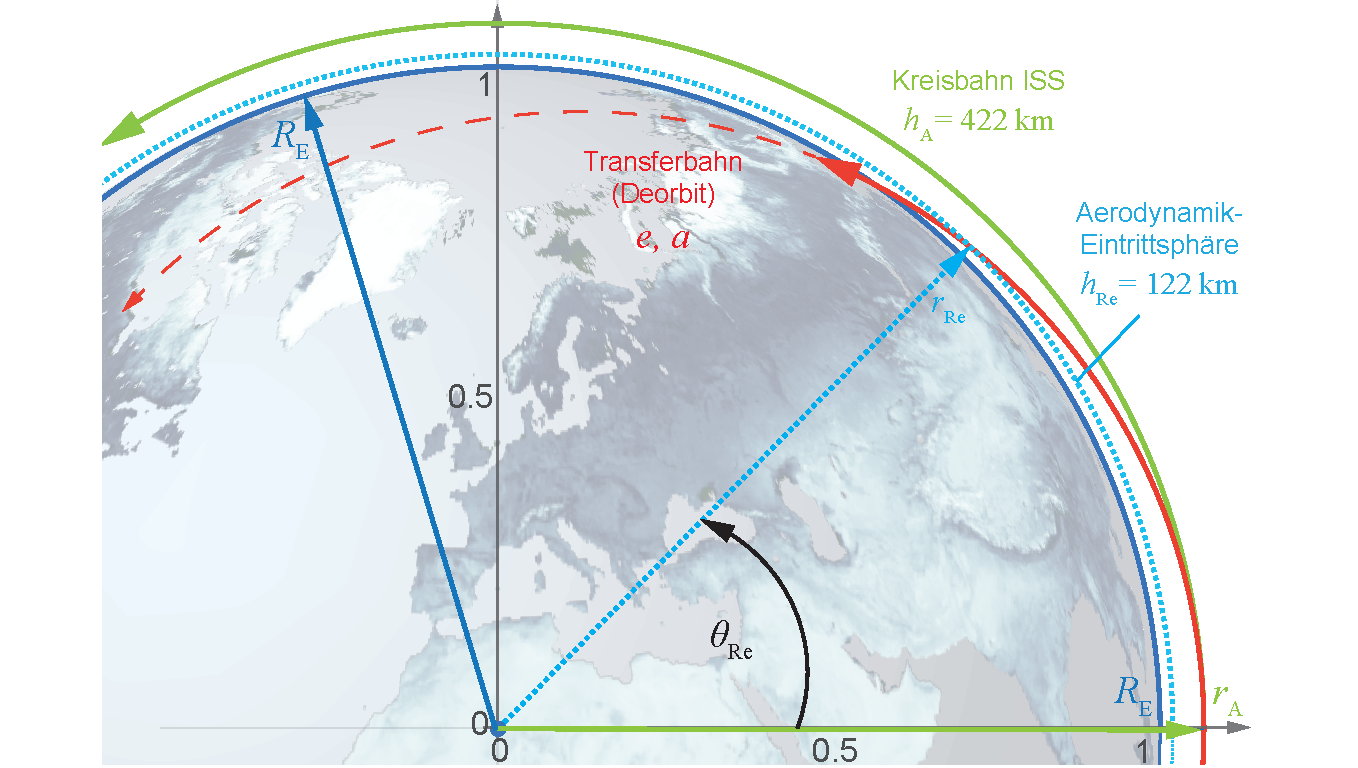
\includegraphics[width=0.8\textwidth]{ReentryGeometrie01.pdf}
\caption[Wiedereintritt-Transferbahn.]{Wiedereintritt-Transferbahn (Deorbit). Parameter: $r_\text{A} = R_\text{E} + \SI{422}{\km} =\SI{6800}{\km}$, $q=1.0462$.
Siehe auch \mscr{}\mladynref{Transfer2Reentry.m} f�r weitere Details und Graphiken.}
\label{abb:adyn_reentry02}
\end{figure}

Hier sind $\gamma_\text{Re}$ der FPA und $r_\text{Re}$ der Abstand zum Erdzentrum am �bergangspunkt bekannte Gr��en. Gesucht sind der Bahnparameter $e,\,a, \upsilon_\text{Re}$ der freien Trajektorie bis zum Wiedereintrittspunkt (im Englischen auch \textit{Deorbit}, also Abstiegsbahn genannt), die Geschwindigkeit $v_\text{Re}$ und der notwendigen Antriebsbedarf $\Delta v$ beim Apog�um $\Delta v$ (\figref{adyn_reentry01}). 
Der Drehimpuls der Bahn ist nach \eqref{eq:hm_drehimpuls_von_ae} gegeben durch:  $L=\sqrt{\mu_\text{E}\,a\,\lk 1-e^2\rk}$. Wir setzen  
\begin{align*}
    q=\frac{r_\text{A}}{r_\text{Re}} > 1\,.
\end{align*}
F�r die Berechnung des Wiedereintritts kann $q$ �ber $r_\text{A}$ als bekannt angenommen werden, ebenso wie der  FPA beim Eintritt $\gamma_\text{Re}$. Dieser wird aus Gr�nden der thermischen Belastung  \ia kleiner als $10\degree$ gew�hlt. Aus \eqref{eq:adyn_reentry02} findet man leicht:
\begin{subequations}
\begin{align}
    e &= \frac{q^2-\lk 2q-1\rk\,\cos^2\gamma_\text{Re}}{q^2-\cos^2\gamma_\text{Re}}\,, \\
    v_\text{Re} &= \sqrt{\frac{2\mu_\text{E}}{r_\text{A}}\,\frac{q^2\,(q-1)}{q^2-\cos^2\gamma_\text{Re}} }\,, \\
    \cos \upsilon_\text{Re} &= \frac{(q-1)^2\cos^2\gamma_\text{Re}- q^2\sin^2\gamma_\text{Re}}{(q-1)^2+(2\,q-1)\,\sin^2\gamma_\text{Re}}\,,\\
   \Delta v &= \frac{\mu_\text{E}}{r_\text{A}} - \cos\gamma_\text{Re}\,\frac{v_\text{Re}}{q}\,.
\end{align}\label{eq:adyn_reentry03}
\end{subequations}

\begin{figure}[H]
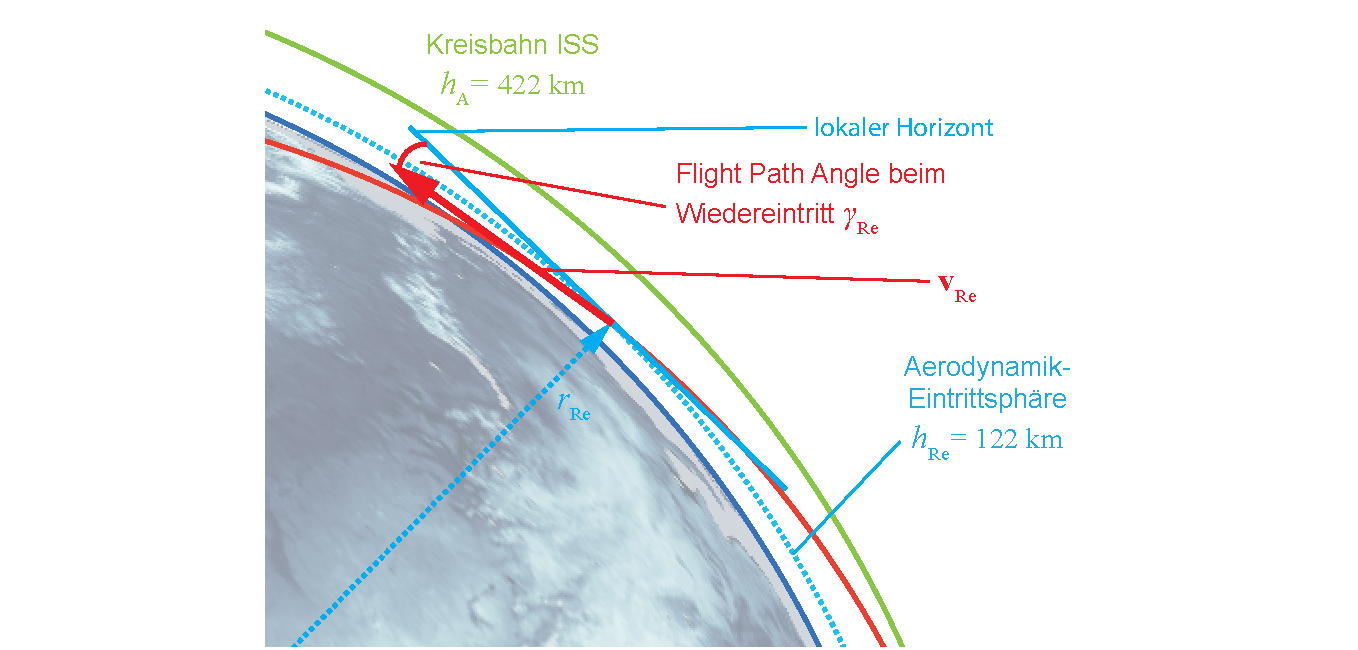
\includegraphics[width=0.95\textwidth]{ReentryGeometrie02.pdf}
\caption[Parameter zur Berechnung der Wiedereintritt-Transferbahn.]{Parameter zur Berechnung der Wiedereintritt-Transferbahn (Deorbit). Die Festlegung von $h_\text{Re}$ auf eine nichtmetrische SI-Einheit $\SI{400000}{}\,\mathrm{ft}$ kommt noch aus der Zeit, da die westliche Raumfahrtwissenschaft sehr stark durch die USA dominiert war. Es sind im �brigen schon Raumfahrtmissionen wegen unterschiedlicher Verwendung nichtmetrischer \bzw imperialer Einheiten und inkorrekter Konversion fehlgeschlagen. Das soll uns nicht passieren, weswegen wir ausschlie�lich das SI-Einheiten-System (siehe die \onlineZ) verwenden.}
\label{abb:adyn_reentry01}
\end{figure}

Wir �berlassen es dem Leser als �bung, die einzelnen Schritte zur Herleitung der Beziehungen \eqref{eq:adyn_reentry02} und \eqref{eq:adyn_reentry03} mit den Kenntnissen aus der Himmelsmechanik \kap{lsg_kepler} nachzuvollziehen (\probref{adyn_reentry01}). \\
Man berechnet nun nach \eqref{eq:adyn_reentry03} schrittweise $e$, $v_\text{Re}$ schlie�lich $\Delta v$ und $\upsilon_\text{Re}$ \bzw $\upsilon_\text{Re}$ =  $\left| \upsilon_\text{Re}- 180\degree \right|$.\\
%F�r diesen Fall und $q= \frac{r_\text{A}}{r_\text{Re}} \to 1$ kann man aus \eqref{eq:adyn_reentry03} eine N�herung erhalten:
%\begin{subequations}
%\begin{align}
    %\upsilon_\text{Re} &= \sqrt{\frac{\mu_\text{E}}{r_\text{A}}} \,\lk 1+\frac{3}{4}\,\lk q-1\rk -\frac{\gamma_\text{Re}{}^2}{8\,\lk q-1\rk}\rk\,,\\
    %\Delta v &= \sqrt{\frac{\mu_\text{E}}{A_\text{A}}}\,\lk q-1 + \frac{\gamma_\text{Re}{}^2}{2\,\lk q-1\rk}\rk
%\end{align}\label{eq:adyn_reentry04}
%\end{subequations}
Als Beispiel sei die R�ckkehr eines Transport-Raumschiffes von der ISS genannt. Man w�hlt einen FPA von $\gamma_\text{Re}=6\degree$ und erh�lt mit $r_\text{A} = R_\text{E} + \SI{422}{\km} =\SI{6800}{\km}$, $q=1.0462$ (siehe \mscr \mladynref{Transfer2Reentry.m} \figref{adyn_reentry02}): 
\begin{align*}
    \theta_\text{Re} = 45.5\degree\,, && v_\text{Re} =  \SI{7.50}{\km\per\second}\,, && \Delta v = -\SI{530}{\metre\per\second}\,.
\end{align*}
Wir k�nnen leicht numerisch oder auch analytisch aus \eqref{eq:adyn_reentry03} ableiten, dass f�r den Wiedereintritt aus einem LEO n�herungsweise gilt:
	\[ q \to 1\,, ~~v_\text{Re} \approx v_\text{K} =\sqrt{\frac{\mu_\text{E}}{R_\text{E}}} = \SI{7.905}{\km\per\second} ~~\text{(1.\,\gls{vkosmos})}\,. \]
Ebenso kann man sich �berlegen, dass f�r einen direkten Wiedereintritt in die Erdatmosph�re aus dem interplanetaren Raum die Anfangsbedingungen lauten: 
	\[ q \to \infty\,,~~ v_\text{Re} \approx \sqrt{\frac{2\mu}{r_\text{Re}}} = \SI{11.8}{\km\per\second} ~~\text{(2.\,\gls{vkosmos})}\,,\\
    ~~~~\upsilon_\text{Re} = 2\,\gamma_\text{Re}\,.\]

\subsubsection{Berechnung der Dynamik des Wiedereintritts in die Erdatmosph�re}

Wir l�sen nun mit den berechneten Anfangsbedingungen die Bewegungsgleichungen f�r die Wiedereintritt-Phase numerisch. Das Ergebnis ist in \figref{adyn_reentry03} und \figref{adyn_reentry04} gezeigt. In der ersten Abbildung ist der "`Gleitpfad"' $h(x)$ f�r zwei verschiedene initiale FPA $\gamma_\text{Re}$ gezeigt. Erwartungsgem�� wird bei einem steilen Eintauchen in die Erdatmosph�re $\gamma_\text{Re} \approx 10\degree$ der Gleitpfad steiler und k�rzer und damit auch die thermische Belastung gr��er. 

\begin{figure}[H]
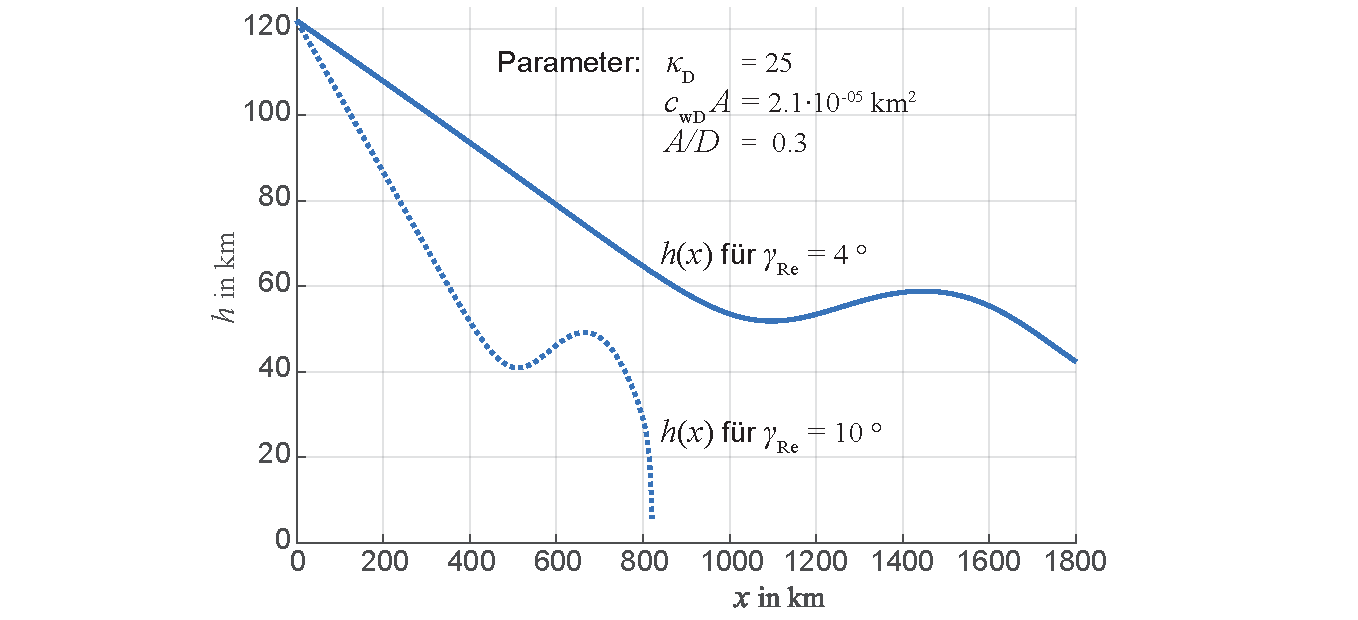
\includegraphics[width=\textwidth]{RaumschiffReentry01.pdf}
\caption[Gleitpfad beim Wiedereintritt.]{Gleitpfad beim Wiedereintritt f�r zwei verschiedene initiale FPA $\gamma_\text{Re}$. Parameter:
$c_\text{D}\cdot A = \SI{1.5}{\metre\squared}$ (Widerstandsbeiwert $\cdot$ Fl�che), $m_\text{L} = \SI{5e3}{\kg}$ (Payload). F�r die Abh�ngigkeit der Dichte von der H�he wurde \eqref{eq:adyn_barom_h_fomulae} verwendet. Siehe auch \mscr{} \mladynref{ReentrySummary.m} f�r weitere Details und Graphiken.}
\label{abb:adyn_reentry03}
\end{figure}

In \figref{adyn_reentry04} sind neben dem H�henverlauf $h(t)$ auch der Geschwindigkeitsverlauf $v(t)$ und die Beschleunigung (Abbremsung) $a(t)$  �ber der Zeit aufgetragen. Deutlich zu erkennen sind die einzelnen Phasen des Abbremsens, so bei $t=50 \ldots 90\,\mathrm{s}$ f�r $\gamma_\text{Re} = 10\degree$ \bzw $t= 100 \ldots 180\,\mathrm{s}$ f�r $\gamma_\text{Re} = 4\degree$. Im zweiten Fall ist also die thermische Belastung (Temperaturerh�hung) auf Grund der doppelt so langen "`Bremszeit"' auf etwa 85\% und die gegebenenfalls durch Astronauten auszuhaltende Maximalbeschleunigung von $20\,g$ auf etwa $5\,g$ reduziert.
\begin{figure}[H]
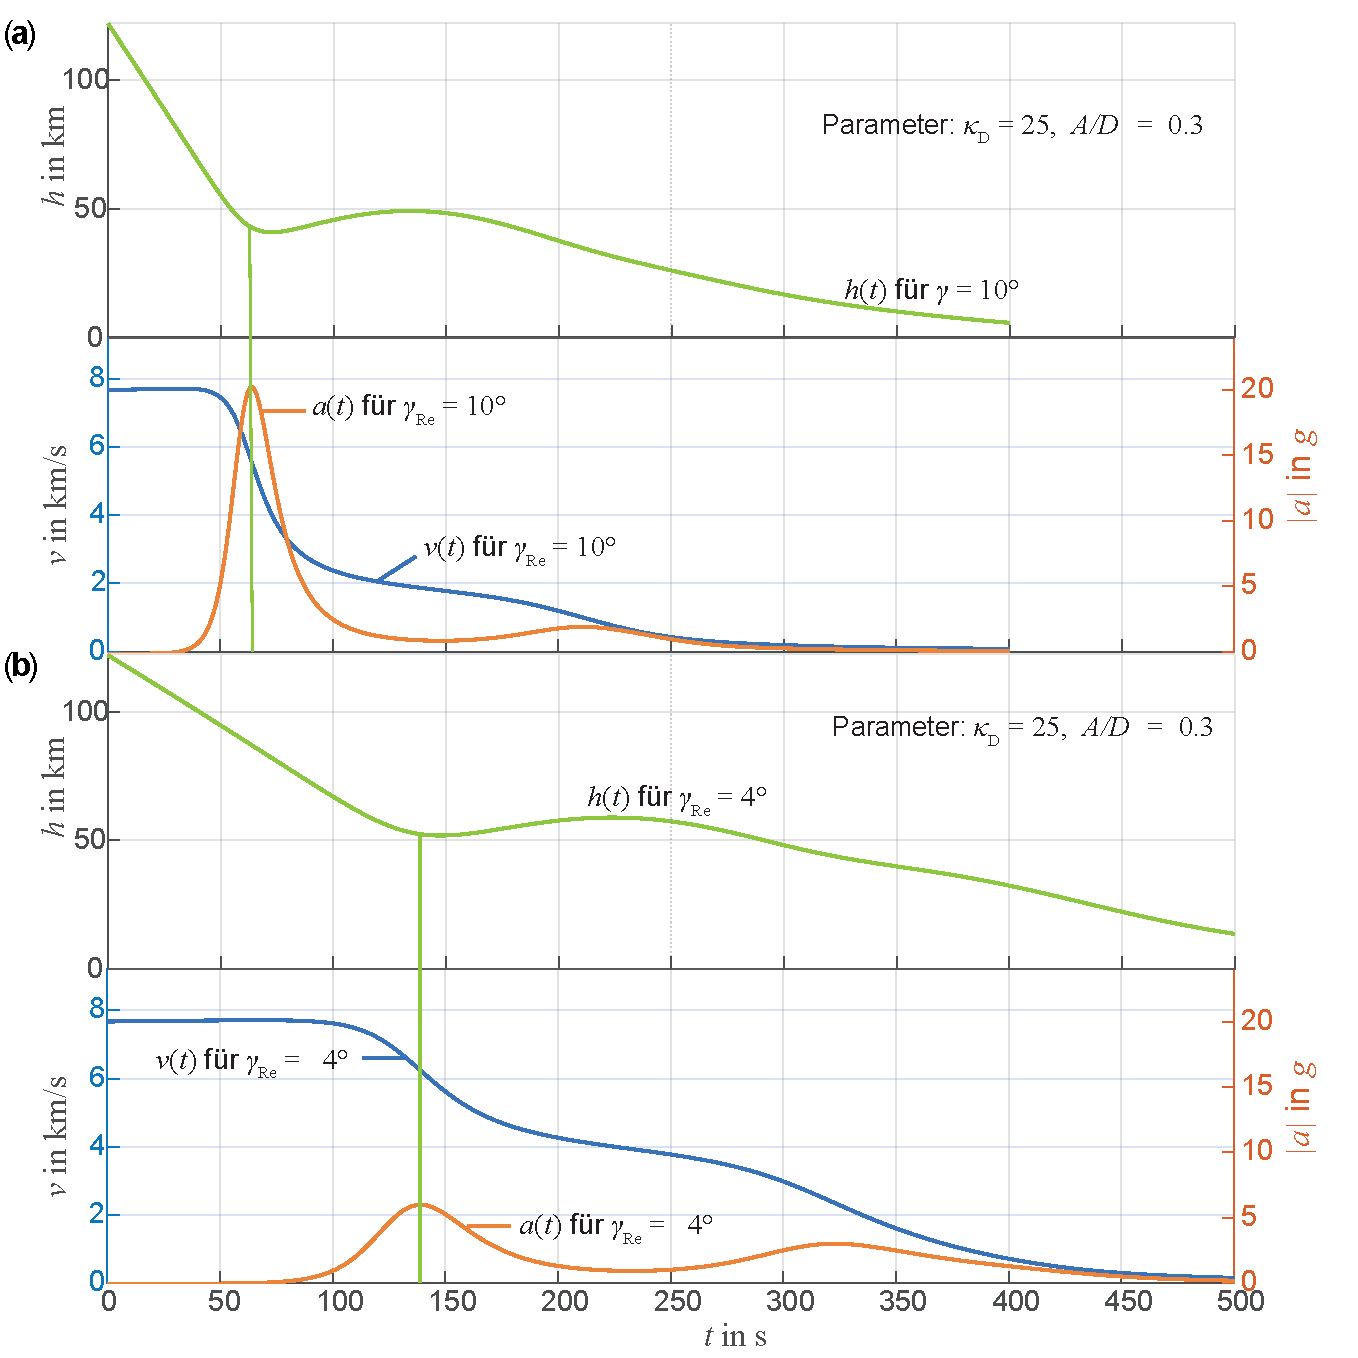
\includegraphics[width=1.0\textwidth]{RaumschiffReentry02.pdf}
\caption[Zeitverl�ufe beim Wiedereintritt.]{Zeitverl�ufe beim Wiedereintritt f�r $h,\, v$ und $a$. Parameter: 
$c_\text{D}\cdot A = \SI{1.5}{\metre\squared}$ (Widerstandsbeiwert $\cdot$ Fl�che), $m_\text{L} = \SI{5e3}{\kg}$ (Payload). F�r die Abh�ngigkeit der Dichte von der H�he wurde \eqref{eq:adyn_barom_h_fomulae} verwendet. \fa initialer FPA $\gamma\text{Re} = 10\degree$,  \fb initialer FPA $\gamma\text{Re} = 4\degree$. Siehe auch \mscr{} \mladynref{ReentrySummary.m} f�r weitere Details und Graphiken.}
\label{abb:adyn_reentry04}
\end{figure}

Ebenso erkennbar sind Phasen ann�hernd konstanter Geschwindigkeit und Phasen in denen es auf Grund eines speziellen Auftrieb/Drag-Verh�ltnisses sogar kurzzeitig zu einem Ansteigen des Raumschiffs kommen kann. Diese Abh�ngigkeit untersuchen wir in \probref{adyn_reentry02}.

\subsubsection{N�herungsformel f�r einzelne Phasen}

Wir wollen nun noch f�r einzelne Phasen des Wiedereintritts einfache N�herungsbeziehungen herleiten. Dabei wenden wir eine h�ufig benutzte Methode an, mit der das noch recht komplexe Differentialgleichungssystem \eqref{eq:adyn_launch08}, in welchem wir wieder den Auftrieb ber�cksichtigen wollen, weiter vereinfacht werden kann. F�r den Drag und den Auftrieb benutzen wir wiederum die barometrische H�henformel 
\begin{align}
    F_\text{D} &= m_\text{R}\,v^2 \frac{\kappa_\text{D}}{H_0} \e^{-h/H_0} ~~~\text{\bzw}~~~
    F_\text{A} = m_\text{R}\,v^2 \frac{\kappa_\text{A}}{H_0} \e^{-h/H_0} \,. \label{eq:adyn_reentry10a}
\end{align}
F�r das Verh�ltnis von Auftrieb zu Drag schreiben wir $A/D = \kappa_\text{A}/\kappa_\text{D}$.
Die Gleichung \eqref{eq:adyn_launch08c} kann benutzt werden um �ber $t=t\lk h\rk$ die Zeitvariable zu eliminieren, womit wir $v\lk h\rk$ und $\gamma\lk h\rk$ bekommen. Gleichzeitig wollen wir zu dimensionslosen Gr��en �bergehen. F�r die Geschwindigkeit schreiben wir $\mu = v/v_\text{K}$ mit $v_\text{k} = \sqrt{\mu_\text{E}/R_\text{E}}$ als die 1.~\gls{vkosmos}. F�r die H�he und Bodendistanz $\eta=h/H_0$ \bzw $\xi=x/H_0$ und f�r die Zeit $\tau= t\,g_\text{E}/v_\text{K}$, worin $g_\text{E}= \mu_\text{E}/R_\text{E}{}^2$ die Erdbeschleunigung auf der Erdoberfl�che ist.
Zum Schluss f�hren wir noch eine dimensionslose spezifische kinetische Energie $\hat{\epsilon}$ ein:
\begin{align}
    \hat{\epsilon} = \mu^2 = \frac{v^2}{v_\text{K}{}^2}~.\label{eq:adyn_reentry10b}
\end{align}
Die dimensionslose H�he $\eta=h/H_0$ skalieren wir exponentiell entsprechend der barometrischen H�henformel zur ebenfalls diemensionslosen H�he $\hat{\eta}$:
\begin{align}
    \hat{\eta} = \frac{2\,\kappa_\text{D}}{\sin\gamma_\text{Re}}\,\e^{-\eta} \;.\label{eq:adyn_reentry10c}
\end{align}
Nach etwas Algebra, die wir in \probref{adyn_reentry03} ausgef�hrt haben, erhalten wir aus \eqref{eq:adyn_launch08}:
\begin{subequations}
\begin{align}
    \frac{\D \lk \ln\hat{\epsilon}\rk}{\D\hat{\eta}} &= -\underbrace{\frac{\sin\gamma_\text{Re}}{\sin\gamma}}_{\text{Drag}}\, + \underbrace{\frac{2H_0}{\hat{\epsilon}\,\hat{\eta}\,R_\text{E}}}_{\text{Gravitation}}\,, \label{eq:adyn_reentry11a}\\
    \frac{\D \lk\cos\gamma\rk}{\D \hat{\eta}} &= \underbrace{\frac{\sin\gamma_\text{Re}}{2}\,\frac{A}{D}}_{\text{Auftrieb}} \,- \underbrace{\lk\frac{1}{\hat{\epsilon}-1}\rk\,\frac{H_0\,\cos\gamma}{\hat{\eta}\,R_\text{E}}}_{\text{Gravitation, Zentrifugalkraft}} \,.\label{eq:adyn_reentry11b}
\end{align} \label{eq:adyn_reentry11}
\end{subequations}

Wir haben zwei Gleichungen erhalten. Die erste beschreibt die Ver�nderung der (dimensionslosen) Energie �ber die dimensionslose H�he und die zweite die Ver�nderung des FPA ebenfalls �ber die dimensionslose H�he.  Auf den ersten Blick sieht das nicht wie ein Fortschritt aus, aber die Gleichungen zeigen eine Separation in vier Terme, die den wirkenden Kr�ften (Auftrieb, Drag, Gravitation und Zentrifugalkraft) zugeordnet werden k�nnen. Aus
\begin{align*}
    a = \frac{\D v}{\D t}= \frac{\D v}{\D \lk\ln\hat{\epsilon}\rk}\,\frac{\D\lk\ln\hat{\epsilon}\rk}{\D\hat{\eta}}\,\frac{\D\hat{\eta}}{\D h}\,\frac{\D h}{\D t}
\end{align*}
folgt
\begin{align}
    a &= \frac{\hat{\epsilon}\,v_\text{K}{}^2}{2v} \,\lek - \frac{\sin\gamma_\text{Re}}{\sin\gamma} + \frac{2H_0}{\hat{\epsilon}\,\hat{\eta}\,R_\text{Re}}\rek\,\lk -\frac{\hat{\eta}}{H_0}\rk\,\lk-v\,\sin\gamma\rk \nonumber \\
    \rightarrow~~~a &= -g_\text{E}\,\lk \frac{\hat{\epsilon}\,\hat{\eta} \,R_\text{E}}{2H_0}\,\sin\gamma_\text{Re} - \sin\gamma\rk\,. \label{eq:adyn_reentry12}
\end{align}
Damit haben wir eine Gleichung gewonnen, die uns erlaubt, abh�ngig von den Parametern $H_0$, $\kappa_\text{D}$, $A/D$ und $\gamma_\text{Re}$ eine Absch�tzung f�r die Beschleunigung zu machen. Wir wollen das an zwei Phasen verdeutlichen:
\subparagraph{Phase ohne Drag}
Wir k�nnen $\kappa_\text{D}\approx 0$ setzen und erhalten aus \eqref{eq:adyn_reentry12}:
\begin{subequations}
\begin{align}
    a &= \dot{v} = g_\text{E}\,\sin\gamma \,,\\
    \dot{\gamma} &= 0\,,\\
    \dot{h} &= -v\,\sin\gamma
\end{align} \label{eq:adyn_reentry13}
\end{subequations}
mit den einfachen L�sungen 
\begin{subequations}
\begin{align}
    \gamma &= \gamma_\text{Re} \,,\\
    h &= h_\text{Re} - v_\text{Re}\,\sin\gamma_\text{Re}\,t \,,\\
    v &= v_\text{Re} + g_\text{E}\,\sin\gamma_\text{Re}\,t\approx v_\text{Re}\,.
\end{align}\label{eq:adyn_reentry14}
\end{subequations}

\begin{figure}[H]
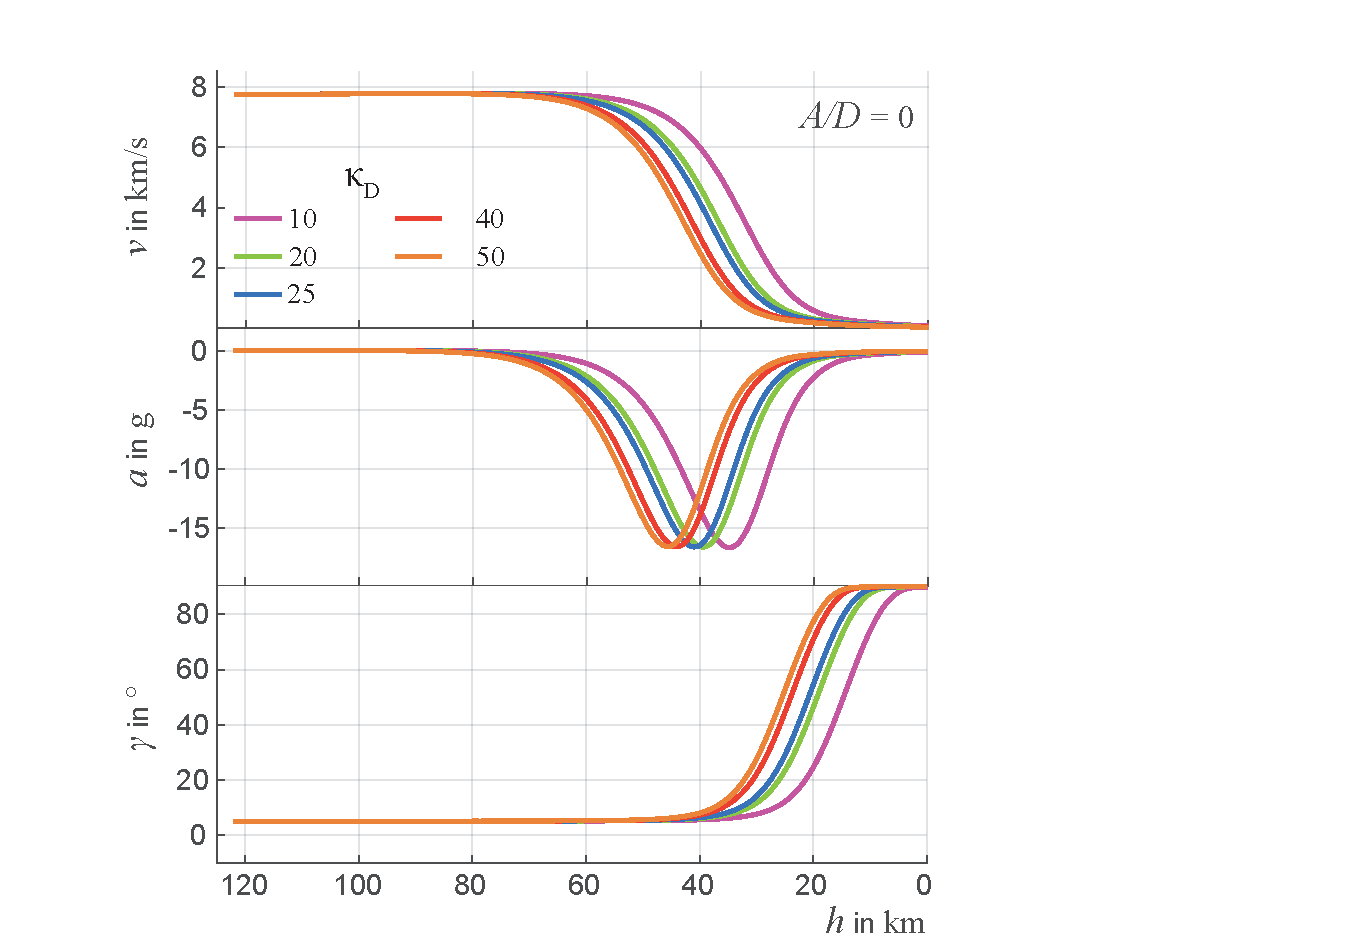
\includegraphics[width=\textwidth]{ReentryNaeherungen01.pdf}
\caption[L�sungen der Bewegungsgleichungen f�r den Wiedereintritt.]{L�sungen der Bewegungsgleichungen f�r den Wiedereintritt f�r verschiedene Reibungskoeffizienten. Siehe auch \mscr{} \mladynref{ReentryNaeherungen.m} f�r weitere Details und Graphiken.}
\label{abb:adyn_reentry05}
\end{figure}

Wir k�nnen das sehr gut in \figref{adyn_reentry05} und \figref{adyn_reentry06} erkennen. Wann aber ist nun das Ende dieser Phase erreicht?
Dazu betrachten wir \eqref{eq:adyn_reentry11a} und sehen, dass $\D \ln\hat{\epsilon} / \D \hat{\eta}< 0$ wird, wenn
\begin{align}
    \frac{\sin\gamma_\text{Re}}{\sin\gamma} = \frac{2H}{\hat{\epsilon}\,\hat{\eta}\,R_\text{E}}\label{eq:adyn_reentry15}\,.
\end{align}
In der initialen Phase ist aber $\hat{\epsilon}\approx 1$ und $\gamma\approx \gamma_\text{Re}$, so dass daraus eine Bedingung f�r $h$ entsteht, bei welcher die sogenannte ballistische Phase beginnt:
\begin{align}
    \hat{\eta} &= \frac{2H_0}{R_\text{E}} ~~ \to ~~ \frac{2\,\kappa_\text{D}}{\sin\gamma_\text{Re}}\,\e^{-\frac{h}{H_0}} = \frac{2H_0}{R_\text{E}} ~~\to ~~ h = -H_0\,\ln\,\frac{H_0\,\sin\gamma_\text{E}}{R_\text{E}\,\kappa_\text{D}}\,.\label{eq:adyn_reentry16}
\end{align}
Wegen $\D \hat{\epsilon} /\D \hat{\eta} = 0 $ ist das auch die H�he, bei der die maximale Geschwindigkeit erreicht wird.

\begin{figure}[H]
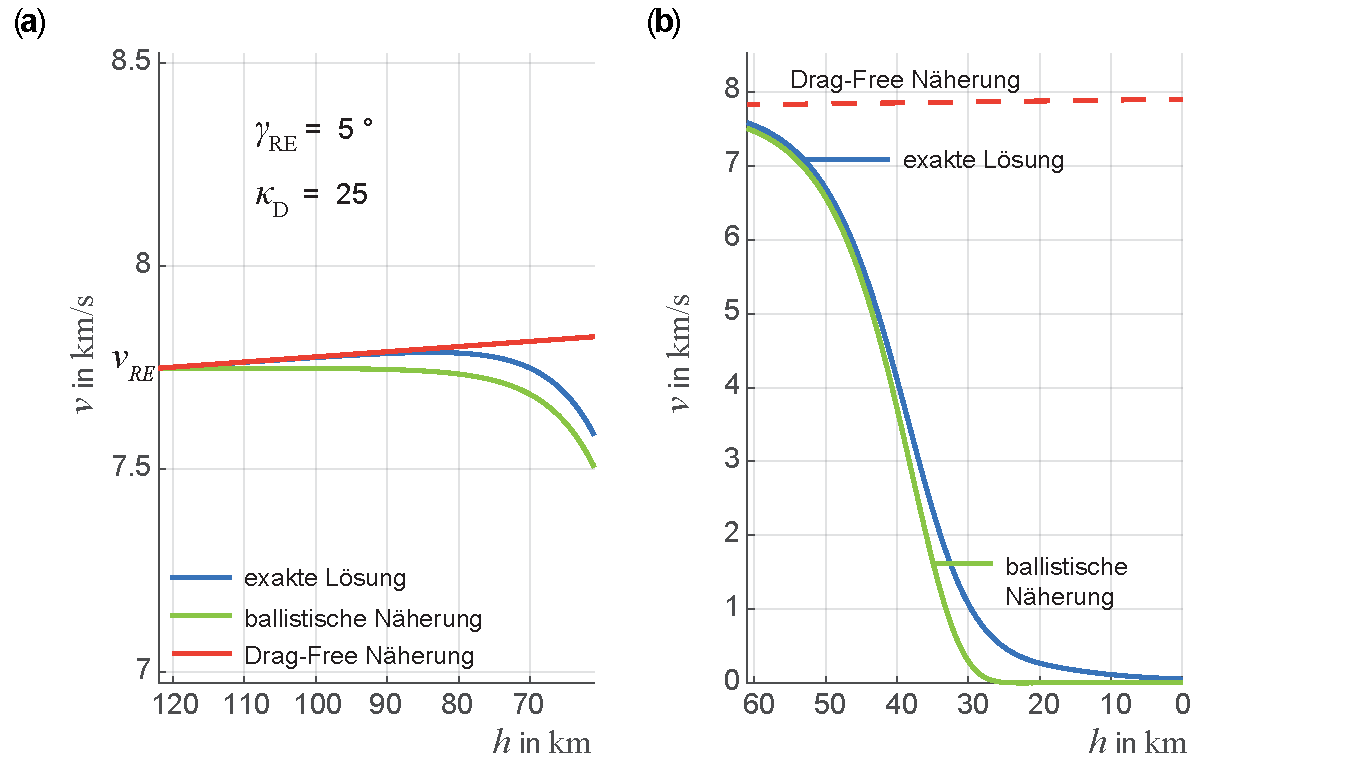
\includegraphics[width=\textwidth]{ReentryNaeherungen02.pdf}
\caption[N�herungsl�sungen normierte Bewegungsgleichungen f�r Wiedereintritt.]{N�herungsl�sungen der normierten Bewegungsgleichungen f�r den Wiedereintritt im Vergleich zur "`exakten"' L�sung. \fa Free-Drag Phase \fb Ballistische Phase. Man erkennt, dass fast unabh�ngig von $\kappa_\text{D}$ die Abbremsung auf eine gleichf�rmige Bewegung in einer H�he von ca. 40 km erfolgt. Siehe auch \mscr{} \mladynref{ReentryNaeherungen.m} f�r weitere Details und Graphiken.}
\label{abb:adyn_reentry06}
\end{figure}

\subparagraph{Ballistische Phase mit gro�em Drag}
Die nachfolgende Phase soll unter der Vereinfachung betrachtet werden, dass alle anderen Kr�fte au�er dem Drag vernachl�ssigt werden k�nnen, \dh $A=0$, $\hat{\epsilon}\approx 1$. 
Dann folgt aus \eqref{eq:adyn_reentry11}:
\begin{align}
\begin{split}
    \frac{\D \ln\hat{\epsilon}}{\D \hat{\eta}} &= -\frac{\sin\gamma_\text{Re}}{\sin\gamma} + \underbrace{\frac{2H_0\,\sin\gamma_\text{Re}}{R_\text{E}\,\kappa_\text{D}}\,\e^{\frac{h}{H_0}}}_{\approx 0}\,,\\
    \frac{\D \cos\gamma}{\D \hat{\eta}} &= 0 \,\,. 
\end{split}   \label{eq:adyn_reentry17}
\end{align}
Das System l�sst sich leicht l�sen und wir erhalten mit $\gamma = \gamma_\text{Re} = \con $ und 
\begin{align}
    \ln\,\frac{\hat{\epsilon}}{\hat{\epsilon}_\text{Re}} &= -\lk\hat{\eta}-\hat{\eta}_\text{Re}\rk \to ~~~ \hat{\epsilon} = \hat{\epsilon}_\text{Re}\,\e^{-\hat{\eta}_0-\hat{\eta}_\text{Re}}\approx\hat{\epsilon}_\text{Re}\,\e^{-\hat{\eta}}\,,\nonumber\\
    v &\approx v_\text{Re}\,\e^{-\frac{\hat{\eta}}{2}} = v_\text{Re}\,\e^{-\lek\frac{\kappa_\text{D}}{\sin\gamma_\text{Re}}\,\e^{-h/H_0}\rek}\,.\label{eq:adyn_reentry18}
\end{align}
Auch diese Phase ist in \figref{adyn_reentry06} gut zu erkennen. \\

Wir m�chten zum Schluss noch einmal darauf hinweisen, dass neben dem Drag auch das nichtsph�rische Gravitationsfeld der Erde und der Strahlungsdruck einen abbremsenden Charakter auf Raumsonden in niedrigen Orbits haben. In \probref{adyn_reentry04} werden wir ein sehr einfaches Modell einer solchen abfallenden, sinkenden Umlaufbahn untersuchen.
Wir konnten mit diesem kurzen Exkurs das hochinteressante Thema des Wiedereintritts von Raumschiffen in die Erdatmosph�re nur anrei�en und m�ssen den interessierten Leser f�r weitere Details an die entsprechende Fachliteratur verweisen \cite{Walter2018, Veris2018}, womit wir dann auch das sch�ne Kapitel der Astrodynamik schlie�en. \\
 
\clearpage
%%% Anmerkung 2023-11-13 (mk.):
%%% Links auf L�sungen komplett auskommentiert, da extra file bew_uebungenAB.tex
%%% Einfaches �ndern durch  ersetzen \hyperref.. <--> %\hyperref.

%%% Links basieren f�r ein m�gliches e_book auf getrennter pdf-Zieldokumente auf pdf-Hypertags:
%%%        \linklsg\\%\href{FingerUeb2_AB.pdf#prb:adyn_canonball}{\textcolor{blue} {$\rightarrow$ zur \probref{adyn_canonball}.}}\\
%%% Einfaches �ndern durch  ersetzen %href{FingerUeb1_AB.pdf.. <--> \linklsg\\%\href{FingerUeb1_AB.pdf..
%%%
%%% oder 
%%% f�r das Arbeitsbuch als geschlossenes Zieldokument auf normalen Verweisen (siehe bew_uebungenAB.tex):
%%%        \textcolor{blue} {$\rightarrow$ zur} \probref{adyn_canonball}.\\
%%%

\section{�bungen zu \autoref{chap:adyn} -- Astrodynamik}\label{kap:adyn_uebungen}

\medskip
Die �bungen sind mit Schwierigkeitsindikatoren markiert, von einfach ($\ast$) �ber mittel ($\ast \ast$) bis schwierig ($\ast \ast \ast$).
Zusatzaufgaben sind zum Teil mit ($\ast \ast \ast \;!$) markiert und eher als Erweiterung des Theorieteils zu betrachten.
Einige wenige �bungen sind rein analytisch, die gro�e Mehrzahl beinhaltet aber \matlab-Anwendungen. \\

L�sungsbeispiele finden sich in den \onlineZ{} im Arbeitsbuch {\textcolor{blue}{FingerUeb2\_AB.pdf}} und k�nnen �ber den Link \linklsg erreicht werden.\\
Die entsprechenden \mscre finden sich im GitHub unter \githubSN \bzw
in den \onlineZ{} (\MKc).\\

%%%-----------------------------------------------------------------------------------------------------------

\subsection{�bungen zu Grundlagen der Raketenphysik}

\medskip

%-----------------------------------------------------------------------------------------------------------

\begin{prob} %�bung1
\einfach{adyn_canonball}{Jules Vernes Kanonenschuss zum Mond}
In seinem Buch "`Von der Erde zum Mond"' berichtet Jules Verne, dass ein Kanonenclub in den USA einen Vorschlag machte, mit einer Kanone ein Geschoss von der Erde zum Mond zu schicken. Man plante eine Granate mit einer Nutzlast von $\SI{8.75}{\tonne}$ und einigte sich auf ein Gesch�tzrohr von $\SI{270}{\metre}$ L�nge aus Gusseisen. Als Treibladung sollte Schie�baumwolle (Zellulosenitrat) verwendet werden. %Als geeigneter Standort f�r die Kanone wurde der Bundesstaat Florida gew�hlt.\\
%Jules Vernes Astronauten starteten also genau so wie die sp�teren NASA-Astronauten in Florida und erneuerten den notwendigen Sauerstoff im Projektil durch Erhitzen von Kaliumchlorat.
Diskutieren Sie die Chancen, die drei Astronauten und zwei Hunde mit dieser Technik sicher zum Mond zu bringen.

\medskip
\linklsg\\%\href{FingerUeb2_AB.pdf#lsg:adyn_canonball}{\textcolor{blue} {$\rightarrow$ L�sungsteil}}.\\
%\hyperref[lsg:adyn_canonball]{\textcolor{blue} {$\rightarrow$ L�sungsvorschlag}}.\\
\noindent\rule[1ex]{\textwidth}{0.5pt}
\end{prob}

%-----------------------------------------------------------------------------------------------------------

\begin{prob} %�bung2
\einfach{adyn_rocketbasic}{Prinzip Mehrstufenrakete}
Man kann einige grunds�tzliche Erkenntnisse aus der Raketen-Gleichung \eqref{eq:adyn_rockets19} ableiten, wenn man \zb den Spezialfall gleicher Stufenmassen und gleicher Massen f�r alle $N$~Raketenstufen betrachtet, also $v_{\text{G},i} = v_\text{G}^*\,,~~ m_{0,i}/(m_{0,i}-m_{\text{T},i}) = \mathcal{M}^*\,$. Man erh�lt aus \eqref{eq:adyn_rockets19}:
\begin{align}
\begin{split}
     \Delta v_\text{ges} &=  N\,v_\text{G}^*\,\ln \mathcal{M}^* ~~\rightarrow ~~  \lk \mathcal{M}^* \rk^N = \e^{\Delta v_\text{ges}/v_\text{G}^*} ~~\text{\bzw} ~~ \mu_\text{L} =  \frac{m_\text{L}}{m_0} = \lk \mathcal{M}^* \rk^{-N}\,,
\end{split}  \label{eq:adyn_rockets20}
\end{align}
was bedeutet, dass das Antriebsverm�gen linear mit der Stufenzahl $N$ zunimmt, w�hrend das Nutzlastverh�ltnis exponentiell mit $N$ f�r diesen speziellen Fall der Massenverh�ltnisse abnimmt. Leiten Sie \eqref{eq:adyn_rockets20} her.

\medskip
%\hyperref[lsg:adyn_rocketbasic]{\textcolor{blue} {$\rightarrow$ L�sungsvorschlag}}.\\
\linklsg\\%\href{FingerUeb2_AB.pdf#lsg:adyn_rocketbasic}{\textcolor{blue} {$\rightarrow$ L�sungsteil}}.\\
\noindent\rule[1ex]{\textwidth}{0.5pt}
\end{prob}

%-----------------------------------------------------------------------------------------------------------

\begin{prob}  %�bung3
\schwierig{adyn_rocketopt1}{Optimierung Mehrstufenrakete (Tandemstufung)}
\begin{enumerate}
	\item \textit{\textbf{\anf{Optimieren} Sie Parameter der dreistufigen Saturn V Rakete mit 100 t Nutzlast �ber die Methode der Extremwertberechnung}}\\
          Nehmen Sie die Ausstr�mgeschwindigkeiten $v_{\text{G},i}$, die Strukturkoeffizienten $\sigma_i$ und die zu transportierende Nutzlast $m_\text{L}$ \bzw das Nutzlastverh�ltnis $\mu_\text{L}$ als gegeben an. Daten finden Sie dazu in Tabelle \ref{tab:adyn_parameter_raketen} im Tabellenanhang \kap{adyn_tabellen}. 
Formulieren Sie das Problem als Extremwertberechnung f�r $\Delta v_\text{g}$ in Abh�ngigkeit von den Massenverh�ltnissen $\mu_i$.\\

	\item \textit{\textbf{Berechnen Sie das erzielbare Nutzlastverh�ltnis der Saturn V Rakete f�r den Flug zum Mond �ber die Methode der der Lagrange-Multiplikatoren}}\\ 
Gehen von einem Antriebsbedarf $\Delta v_\text{g}= \SI{12.4}{\kilo\metre\per\second}$ aus. Vergleichen Sie Ihr Ergebnis mit dem tats�chlich von der NASA realisierten Nutzlastverh�ltnis.
F�r die Apollo 11 Mission w�hlte die NASA folgende Konfiguration der Saturn V Rakete (siehe Tab. \ref{tab:adyn_parameter_Apollo11}), um eine Nutzlast von $\SI{47000}{\kg}$ zum Mond zu bringen:
\begin{table}%tab1
\caption[Saturn V Konfiguration f�r die Apollo 11 Mission.]{Saturn V Konfiguration f�r die Apollo 11 Mission \cite{Walter2018}.}
\smallskip
\hspace{1.5cm}
\begin{tabular}{L{1.5cm}R{2cm}R{2cm}R{2cm}R{1.5cm}}
\svhline\noalign{\smallskip}
Gr��e				    			& 1. Stufe				& 2. Stufe   	    & 3. Stufe  		& Einheit \\
\noalign{\smallskip}\svhline\noalign{\smallskip}
\noalign{\smallskip}
$m_{0,i}$							&	$\SI{2902000}{}$	&	$\SI{ 658000}{}$	&	$\SI{  165000}{}$	&	$\SI{}{\kg}$	 \\	
$v_{\text{G},i}$			&	$\SI{  2980}{}$	&	$\SI{   4130}{}$	&	$\SI{    4130}{}$	&	$\SI{}{\metre\per\second}$	 \\	
$\sigma_i$						&	$\SI{0.0765}{}$	&	$\SI{0.1140}{}$	&	$\SI{0.1110}{}$	&	$\SI{}{}$	 \\	
\noalign{\smallskip}
\svhline\noalign{\smallskip}
\end{tabular} 
\label{tab:adyn_parameter_Apollo11}
\end{table}%tab1
\end{enumerate}

\medskip
%\hyperref[lsg:adyn_rocketopt1]{\textcolor{blue} {$\rightarrow$ L�sungsvorschlag}}.\\
\linklsg\\%\href{FingerUeb2_AB.pdf#lsg:adyn_rocketopt1}{\textcolor{blue} {$\rightarrow$ L�sungsteil}}.\\
\noindent\rule[1ex]{\textwidth}{0.5pt}
\end{prob}

%-----------------------------------------------------------------------------------------------------------
\begin{prob}  %�bung4
\einfach{adyn_rocketopt2}{Vergleich Mehrstufenrakete (Serielle und Parallelstufung)} 
Stellen Sie die Vor- und Nachteile der Parallelstufung gegen�ber der Tandemstufung einer Mehrstufenrakete zusammen.

\medskip
%\hyperref[lsg:adyn_rocketopt2]{\textcolor{blue} {$\rightarrow$ L�sungsvorschlag}}.\\
\linklsg\\%\href{FingerUeb2_AB.pdf#lsg:adyn_rocketopt2}{\textcolor{blue} {$\rightarrow$ L�sungsteil}}.\\
\noindent\rule[1ex]{\textwidth}{0.5pt}
\end{prob}

%-----------------------------------------------------------------------------------------------------------
%-----------------------------------------------------------------------------------------------------------
\newpage
\subsection{�bungen zu Umlaufbahnen}

\medskip

%-----------------------------------------------------------------------------------------------------------

\begin{prob}  %�bung5
\mittel{adyn_orbits1}{Bahnparameter aus Bodenbeobachtungen}
Berechnen Sie die Bahnparameter f�r die Satelliten mit den folgenden gemessenen geozentrischen Orts- und Geschwindigkeitsdaten:\\
   Satellit 1 (HEO) 
\begin{align*}
   \vec{r}  &= [12000,\,32000,\,-6000]\,\SI{}{\km}\,, \\
	 \vec{v}  &= [1.250,\,1.3,\,-0.2]\,\SI{}{\km\per\second}\,.
\end{align*}
   Satellit 2 (LEO, fast kreisf�rmig, geringe Neigung) 
\begin{align*}
   \vec{r}  &= [6600,\,5800,\,-1000]\,\SI{}{\km}\,, \\
	 \vec{v}  &= [-4.2,\,4.9,\,-0.2]\,\SI{}{\km\per\second}\,.
\end{align*}
Berechnen Sie die Bahnparameter der ISS (am 20.3.2023 UTC 12:00) aus den folgenden ver�ffentlichten geozentrischen Orts- und Geschwindigkeitsdaten der NASA \url{https://spotthestation.nasa.gov/trajectory_data.cfm}:\footnote{Man beachte die Genauigkeiten mit der die Daten von der NASA angegeben werden.}
\begin{align*}
    \vec{r}  &= [-4804.680472139880,\,-4787.203226753670,\,418.697383172504]\,\SI{}{\km}\,, \\
	  \vec{v}  &= [3.084667418034520,\,-3.63637959795974,\,-5.99889734723948]\,\SI{}{\km\per\second}\,. 
\end{align*}

\medskip
%\hyperref[lsg:adyn_orbits1]{\textcolor{blue} {$\rightarrow$ L�sungsvorschlag}}.\\
\linklsg\\%\href{FingerUeb2_AB.pdf#lsg:adyn_orbits1}{\textcolor{blue} {$\rightarrow$ L�sungsteil}}.\\
\noindent\rule[1ex]{\textwidth}{0.5pt}
\end{prob}


%-----------------------------------------------------------------------------------------------------------
\begin{prob}  %�bung6
\einfach{adyn_orbits2}{Bodenspuren von Erdsatelliten}
\begin{enumerate}
\item \textit{\textbf{Bodenspuren verschiedener Satellitenarten (Epoche 01.01.2000)}} 
	\begin{itemize}
			\item Berechnen Sie die Bodenspur eines GEO-artigen-Satelliten.
			\item Berechnen Sie die Bodenspur eines HEO-Satelliten \zb vom Typ Molnija.
			\item Berechnen Sie die Bodenspur eines polaren Satelliten. 
	\end{itemize}

	Benutzen Sie folgende Bahnparameter: \\
	GEO-artig:\, $a = \SI{25000}{\km},\, e = 0.73,\, i = 8\degree,\, \Omega =45\degree$\,, \\
	HEO (Typ Molnija):\, $a = \SI{26555}{\km},\, e = 0.72,\, i = 63.4\degree,\, \Omega =120\degree,\,\omega =270\degree$\,,\\
	Polar-Satellit:\, $a = \SI{7330}{\km},\, e = 0.0,\, i = 93\degree,\, \Omega =130\degree,\,\omega =0\degree$.\\

\item \textit{\textbf{Bodenspuren verschiedener Satelliten in geosynchronen Umlaufbahnen (Epoche 01.01.2000)}}\\
\begin{itemize}
	\item 	Satellit 1:\, $e = 0.2,\, i = -20\degree,\, \Omega =+30\degree,\,\omega =360\degree$\,,
	\item		Satellit 2:\, $e = 0.2,\, i = -30\degree,\, \Omega =-35\degree,\,\omega =+35\degree$\,,
	\item		Satellit 3:\, $e = 0.2,\, i = +45\degree,\, \Omega =-90\degree,\,\omega =-30\degree$.
\end{itemize}
Erkl�ren Sie die Formen der Bodenspuren. Welchen Zusammenhang erkennen Sie? \\

\newpage
\item \textit{\textbf{Berechnen Sie die Bodenspur der ISS mit den Ergebnissen von \probref{adyn_orbits1}}} (Aufnahme zur vom Erdboden sichtbaren ISS siehe \figref{adyn_ISS}).\\
\begin{figure} 
\includegraphics[width=0.85\textwidth]{ISS_ueber_Dresden_2020-05-17.jpg}
\caption[�berflug der ISS �ber dem Altstadtpanorama von Dresden.]{�berflug der ISS am 17.5.2020 um 22:18 Uhr �ber der Altstadt von Dresden. Die Aufnahme besteht aus 20 zusammengesetzten Einzelaufnahmen. W�hrend der Gesamtbelichtung von ca. 2.5 min erzeugen die Fixsterne bereits deutliche Sternspuren. Aufnahme U. Potthoff.}\label{abb:adyn_ISS}
\end{figure}
\end{enumerate}
\medskip
%\hyperref[lsg:adyn_orbits2]{\textcolor{blue} {$\rightarrow$ L�sungsvorschlag}}.\\
\linklsg\\%\href{FingerUeb2_AB.pdf#lsg:adyn_orbits2}{\textcolor{blue} {$\rightarrow$ L�sungsteil}}.\\
\noindent\rule[1ex]{\textwidth}{0.5pt}
\end{prob}

%-----------------------------------------------------------------------------------------------------------

\begin{prob}  %�bung7
\schwierig{adyn_orbits3}{Bodenbeobachtung von Erdsatelliten}
Berechnen Sie die topozentrischen Beobachtungsdaten f�r einen polaren Satelliten von Mitteleuropa aus. Die Bahnparameter sind gegeben durch:
\begin{align*}
	&\text{Bahnh�he}\,\,h & \SI{900}{\km}\\
	&\text{Exzentrizit�t}\,\,e & 0.00\\
	&\text{Bahnneigung} \,\,i &  95 \degree\\
	&\text{Knoten} \,\, \Omega & 135 \degree \, \text{am 1.1.2020}
\end{align*}
Die Stationskoordinaten sind:\\
G�rlitz (D): $~\lambda = 15\degree\,\text{O},\, \varphi = 51\degree\,\text{N}$  und Marienhamn (S): $~\lambda = 20\degree\,\text{O},\, \varphi = 60\degree\,\text{N}$ .\\
$\theta_0$ sei durch die Beziehung \eqref{eq:adyn_orbit06} mit $\theta_0 = 280.4606\degree + 360.9856473\degree \cdot \lk \mathrm{MJD} - 51544.5\rk$ gegeben. Eine Sichtbarkeit des Satelliten ist nur f�r $h>0$ gegeben. \\

\textit{\textbf{Zusatzaufgabe:}} Berechnen Sie die topozentrischen Beobachtungsdaten f�r die ISS mit den Ergebnissen von \probref{adyn_orbits1} f�r zwei Beobachtungsorte und Zeiten. 
Die Stationskoordinaten sind: Kapstadt (RSA): $~\lambda = 18.5\degree\,\text{O},\, \varphi = 34\degree\,\text{S}$  und Mombasa (Kenia): $~\lambda = 40.0\degree\,\text{O},\, \varphi = 04\degree\,\text{S}$.\\
F�r welchen Ort und welche Zeit k�nnen Sie von einer guten Beobachtungschance ausgehen?  Was k�nnen Sie zu den Beobachtungsdauern sagen?

\medskip
%\hyperref[lsg:adyn_orbits3]{\textcolor{blue} {$\rightarrow$ L�sungsvorschlag}}.\\
\linklsg\\%\href{FingerUeb2_AB.pdf#lsg:adyn_orbits3}{\textcolor{blue} {$\rightarrow$ L�sungsteil}}.\\
\noindent\rule[1ex]{\textwidth}{0.5pt}
\end{prob}

%-----------------------------------------------------------------------------------------------------------

\begin{prob}  %�bung 8
\mittel{adyn_orbits4}{Bodenbeobachtung eines Molniya HEO-Satelliten}
Berechnen Sie die m�glichen Bodenbeobachtungen eines Molniya HEO-Satelliten: Die Bahnparameter sind gegeben durch
\begin{align*}
	&\text{Gro�e Halbachse}\,\,h & \SI{26555}{\km}\,\\
	&\text{Exzentrizit�t}\,\,e & 0.72\, \\
	&\text{Bahnneigung} \,\,i &  63.4 \degree\, \\
	&\text{Knoten} \,\, \Omega & 125 \degree \,\\ 
	&\text{Argument Perig�um} \,\, \omega & 270 \degree \,\\ 
	&\text{Mittlere Anomalie} \,\, M & 0 \degree \,
\end{align*}
Die Stationskoordinaten sind:\\
Indien: $~\lambda = 75\degree\,\text{O},\, \varphi = 10\degree\,\text{N}$  und Russland: $~\lambda = 75\degree\,\text{O},\, \varphi = 55\degree\,\text{N}$ .\\
Die Beobachtungszeiten seien von 11.03.2020\,16:00:00 UTC bis 12.03.2020\,04:00:00 UTC\,.\\

Erkl�ren Sie Ihre Berechnungen und an Hand Ihrer Graphiken, warum der Satellit sehr geeignet ist f�r die Nachrichten�bertragung in hohe geographische Breiten.\\

\textit{\textbf{Zusatzaufgabe:}} Berechnen Sie mit den Kenntnissen aus \kap{adyn_lambert_transfer} und den Ergebnissen von \probref{adyn_manoevers4} in Umkehrung aus den topozentrischen Beobachtungsdaten zu zwei verschiedenen und Zeiten die Bahnparameter (siehe auch \probref{adyn_orbits_zusatz1}). 

\medskip
%\hyperref[lsg:adyn_orbits4]{\textcolor{blue} {$\rightarrow$ L�sungsvorschlag}}.\\
\linklsg\\%\href{FingerUeb2_AB.pdf#lsg:adyn_orbits4}{\textcolor{blue} {$\rightarrow$ L�sungsteil}}.\\
\noindent\rule[1ex]{\textwidth}{0.5pt}
\end{prob}

%-----------------------------------------------------------------------------------------------------------

\begin{prob}  %�bung 9
\mittel{adyn_orbits5}{Sonnensynchrone Bahnen}
Bestimmte Satelliten, wie \zb die Wettersatelliten wie METOP\footnote{METOP ist eine Serie von drei europ�ischen Wettersatelliten.} oder Erderkundungssatelliten wie Landsat\footnote{Landsat-Satelliten sind zivile Erdbeobachtungssatelliten der NASA zur Erkundung der Erdoberfl�che und der K�stenregionen.}, bewegen sich auf einer sogenannten \textit{sonnensynchronen Umlaufbahn} (englisch \textit{Sun Synchronous Orbit} -- SSO, siehe \figref{adyn_synchron_orbit_uebung})\index{Umlaufbahn!sonnensynchrone}. Bei einer solchen Umlaufbahn um die Erde hat die Bahnebene immer den gleichen Winkel zur Linie Erdmittelpunkt-Sonne. Wegen des Umlaufs der Erde um die Sonne kann das nur sein, wenn die Bahnebene die gleiche Rotations�nderung erf�hrt wie die Erde um die Sonne, \dh die Bahnebene des Satelliten sich in einem Jahr einmal um die Erde dreht, wobei diese kontinuierliche �nderung der Bahnebene nicht durch ein Steuerungsman�ver realisiert werden kann!\\

\begin{figure}[H]
	\includegraphics[width=\textwidth]{SonnensynchroneBahn.pdf} 
	\caption[Sonnensynchrone Bahn.]{[Sonnensynchrone Bahn. Symbolische und nicht-ma�stabsgetreue Darstellung. }
	\label{abb:adyn_synchron_orbit_uebung}
\end{figure}

Wie ist das dann aber mit dem Drehimpulserhaltungssatz in Einklang zu bringen? Denken Sie dabei an St�rungen, die durch die abgeplattete Erde hervorgerufen werden.

\textbf{Zusatzaufgabe}\\
Berechnen Sie die Bodenspur eines der fr�hen SSO-Satelliten (ERS-1) der ESA.\footnote{Diese European Remote Sensing Satellites ERS dienten der Fernerkundung der Erdoberfl�che und sind heute nicht mehr in Betrieb. ERS-1 war dabei der erste Erdbeobachtungssatellit der ESA und eine ihrer wichtigsten Satellitenentwicklungen der 1980er Jahre. Start war 17.07.1991, Missionsende am 10.03.2000.} 
Der nahezu kreisf�rmige Orbit war Anfangs so ausgelegt, dass die geographische L�nge des �quator-Durchgangs sich nach 3 Tagen und insgesamt 43 Umrundungen immer wiederholte. Sp�ter wurde der Satellit auf eine sonnensynchrone Bahn mit 782\,x\,785\,km und $98.5\degree$ mit einem Wiederholzyklus von 35 Tagen gebracht \cite{Gottschalk1991, Montenbruck2012}.

\medskip
%\hyperref[lsg:adyn_orbits5]{\textcolor{blue} {$\rightarrow$ L�sungsvorschlag}}.\\
\linklsg\\%\href{FingerUeb2_AB.pdf#lsg:adyn_orbits5}{\textcolor{blue} {$\rightarrow$ L�sungsteil}}.\\
\noindent\rule[1ex]{\textwidth}{0.5pt}
\end{prob}



%-----------------------------------------------------------------------------------------------------------
\newpage
\begin{prob}   %�bung 10
\mittel{adyn_starlink}{Starlink}
Starlink ist ein von dem US-Raumfahrtunternehmen SpaceX betriebenes Satellitennetzwerk, das seit 2020 in verschiedenen Ausbaustufen Internetzugang bietet, seit 2023 weltweit. 
Wenn das Projekt komplett realisiert wird, f�llt sich in den
n�chsten Jahren der Himmel mit einer gewaltigen Zahl von Kommunikationssatelliten und wird auch den Anblick unseres Nachthimmels ver�ndern. 
Mit 4845 Starlink-Satelliten im Erdorbit (Stand Ende September 2023) ist SpaceX bereits heute der mit Abstand gr��te Satellitenbetreiber weltweit (siehe \figref{adyn_starlink01}). Insgesamt bestehen Genehmigungen f�r den Start von maximal 19.427 Satelliten, sowie Antr�ge von SpaceX f�r nochmals bis zu 22.488 Satelliten. Zusammen entspricht das der fast der f�nffachen Zahl aller von 1957 (Sputnik 1) bis 2023 gestarteten Satelliten.\footnote{Seit Sputnik 1 hat die Menschheit \ca 10000 Objekte ins All gebracht. Aktuell befinden sich noch etwas weniger als 6000 im Erdorbit, der Rest ist zur�ck zur Erde gekehrt oder in der Atmosph�re vergl�ht.}
\begin{figure}[H]
	\includegraphics[width=0.9\textwidth]{Starlink01.pdf} 
	\caption[Starlink (Himmelspur und k�nstlerische Darstellung).]{Starlink. Map aller gestarteter Starlink-Satelliten \url{https://satellitemap.space} und Aufnahme der Himmelspur eines Zuges von Starlink-Satelliten �ber Dresden (Aufnahme: U. Potthoff). Die gro�e Anzahl von Starlink-Satelliten stellt durchaus eine Beeinflussung astronomischer Beobachtungen dar. Siehe dazu auch \cite{FAZ2020} und \url{https://findstarlink.com}.}
	\label{abb:adyn_starlink01}
\end{figure}

SpaceX wird das Projekt mit Satelliten in zun�chst drei "`Kugelschalen"' umsetzen, und zwar in H�hen von $h_1= \SI{340}{\km}$, $h_2= \SI{550}{\km}$ und $h_3= \SI{1200}{\km}$ mit jeweils $N_i=7518,\, 1584,\,2825$ Satelliten. Durch diese sollen auch die entlegensten
Orte der Erde mit dem Internet versorgt werden. Wir wollen einige Fakten zu Starlink berechnen (Aufgabe nach \cite{Quetz2019}, mit freundlicher Genehmigung):
\begin{enumerate}
	\item Berechnen Sie die Anzahl der Satelliten, die f�r einen beliebigen Beobachter auf der Erdoberfl�che ($h_\text{B}=0$ und Refraktion vernachl�ssigt) st�ndig sichtbar sind. Wie viele Starlink-Satelliten sind insgesamt -- alle Schalen zusammengenommen -- dann oberhalb des Horizonts? Wir nehmen dabei an, dass die Satelliten in gleichm��igen Abst�nden zueinander fliegen. 
	\item Welcher mittleren Raumwinkeldichte entspricht diese Anzahl? Vergleichen Sie diese anschaulich mit anderen Himmelsobjekten. Wie viel Zeit braucht ein Starlink-Satellit in der jeweiligen Schale um "`vor"' dem Mond vorbei zu fliegen.
%	\item Wenn man die Polarregion ($\left|\varphi\right| > 70\degree$) "`ausspart"', \dh keine Abdeckung dort erreicht, erh�ht sich logischerweise die Zahl der sichtbaren Satelliten �ber dem Horizont in den Regionen ($\left|\varphi\right| < 70\degree$). Um wie viel? Was w�rde es kosten, diese d�nn besiedelten Regionen auch noch abzudecken, wenn ein ein Satellit 250000 USD und jeder Start mit jeweils 60 Satelliten 50 Millionen USD kostet?
\end{enumerate}
Diese Aufgabe wurde zuerst in �hnlicher Form in \cite{Quetz2019} gestellt.\\

\medskip
%\hyperref[lsg:adyn_starlink]{\textcolor{blue} {$\rightarrow$ L�sungsvorschlag}}.\\
\linklsg\\%\href{FingerUeb2_AB.pdf#lsg:starlink}{\textcolor{blue} {$\rightarrow$ L�sungsteil}}.\\
\noindent\rule[1ex]{\textwidth}{0.5pt}
\end{prob}


\newpage
%-----------------------------------------------------------------------------------------------------------
\subsection{�bungen zu Man�vern im Weltall}
\medskip

%-----------------------------------------------------------------------------------------------------------
\begin{prob}  %�bung11
\einfach{adyn_rocket_analogy}{Analogie zum Oberth-Effekt der Astrodynamik}

(Nach \cite{Blanco2019}.)\\
Stellen Sie sich ein Raketenauto nach \figref{adyn_rocket_analogy01} vor. Es f�hrt in die Mulde (tiefster Punkt bei B) bei Punkt A ein (mit einer vernachl�ssigbaren Anfangsgeschwindigkeit) und soll nach M�glichkeit den Punkt C erreichen. An welchem Punkt der Fahrt ist es sinnvoll, die Rakete zu z�nden? Welches Antriebsverm�gen muss diese mindestens haben? Die Reibung sei vernachl�ssigt. \\
Beschreiben Sie mit dieser Analogie den Oberth-Effekt der Astrodynamik.

\begin{figure}[H]
	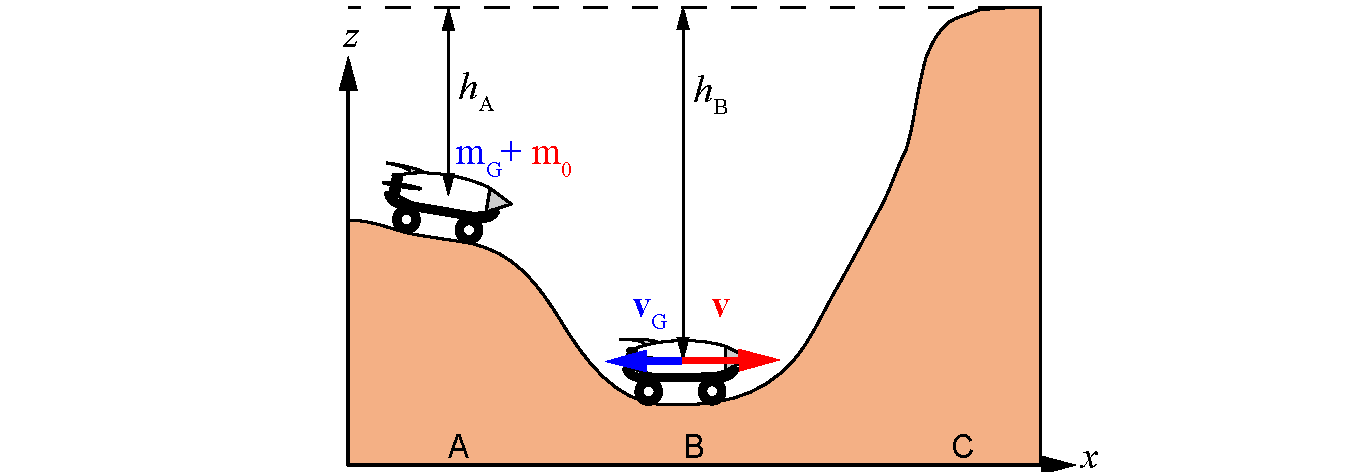
\includegraphics[width=\textwidth]{OberthEffAnalogie.pdf} 
	\caption[Analogie-Modell zum Oberth-Effekt.]{Analogie-Modell zum Oberth-Effekt (nach \cite{Blanco2019}).}
	\label{abb:adyn_rocket_analogy01}
\end{figure}

\medskip
%\hyperref[lsg:adyn_rocket_analogy]{\textcolor{blue} {$\rightarrow$ L�sungsvorschlag}}.\\
\linklsg\\%\href{FingerUeb2_AB.pdf#lsg:adyn_rocket_analogy}{\textcolor{blue} {$\rightarrow$ L�sungsteil}}.\\
\noindent\rule[1ex]{\textwidth}{0.5pt}
\end{prob}

%-----------------------------------------------------------------------------------------------------------

\begin{prob}  %�bung12
2
\einfach{adyn_manoevers1}{Hohmann-Transfer}
Berechnen Sie die �bergangszeit f�r den Hohmann-Transfer als Funktion von $r_2/r_1$ und diskutieren Sie diese.\\
Erkl�ren Sie, warum $\Delta v$ f�r den Hohmann-Transfer in bestimmten Situationen gr��er sein kann als die \gls{vescape}, obwohl die Bahn ja noch eine geschlossene Kreisbahn bleibt.\\ 
Was k�nnen Sie zu $\Delta v$ sagen, wenn man den Bahnradius verkleinern will?

\medskip
%\hyperref[lsg:adyn_manoevers1]{\textcolor{blue} {$\rightarrow$ L�sungsvorschlag}}.\\
\linklsg\\%\href{FingerUeb2_AB.pdf#lsg:adyn_manoevers1}{\textcolor{blue} {$\rightarrow$ L�sungsteil}}.\\
\noindent\rule[1ex]{\textwidth}{0.5pt}
\end{prob}

\newpage
%-----------------------------------------------------------------------------------------------------------
\begin{prob}  %�bung13
\mittel{adyn_manoevers2}{Bielliptischer �bergang}

Zwei-Impuls-�bergang von Bahn mit Radius $r_1$ auf eine elliptische Bahn mit Radius $r_2$:
Da der Antriebsbedarf $\Delta v$ beim Hohmann-Transfer in bestimmten F�llen sehr gro� sein kann, kann man �berlegen, ob es nicht g�nstiger ist, dass Raumschiff zun�chst auf die \gls{vescape} zu beschleunigen und dann wieder abzubremsen. Zeigen Sie, dass das in der Tat so sein kann. Was ist der Nachteil eines solchen Man�vers?

\medskip
%\hyperref[lsg:adyn_manoevers2]{\textcolor{blue} {$\rightarrow$ L�sungsvorschlag}}.\\
\linklsg\\%\href{FingerUeb2_AB.pdf#lsg:adyn_manoevers2}{\textcolor{blue} {$\rightarrow$ L�sungsteil}}.\\
\noindent\rule[1ex]{\textwidth}{0.5pt}
\end{prob}

%-----------------------------------------------------------------------------------------------------------
\begin{prob}  %�bung14
\einfach{adyn_manoevers3}{Hohmann-Oberth-Edelbaum-Transfers aus dem Orbit nach $\infty$}
Berechnen Sie Antriebsbedarfe und Energiegewinne eines Raumschiffs f�r die verschiedenen impulsiven Man�ver. F�r welchen Transfer w�rden Sie sich entscheiden, wenn der Treibstoffvorrat begrenzt ist?\\
Berechnen Sie die Flugzeiten des Raumschiffs bei den verschiedenen impulsiven Man�vern, bis das Raumschiff eine Entfernung des 50-, 100- \bzw 200-fachen des Radius~$r_1$ der anf�nglichen Umlaufbahn hat.

\medskip
%\hyperref[lsg:adyn_manoevers3]{\textcolor{blue} {$\rightarrow$ L�sungsvorschlag}}.\\
\linklsg\\%\href{FingerUeb2_AB.pdf#lsg:adyn_manoevers3}{\textcolor{blue} {$\rightarrow$ L�sungsteil}}.\\
\noindent\rule[1ex]{\textwidth}{0.5pt}
\end{prob}

%-----------------------------------------------------------------------------------------------------------
\begin{prob}  %�bung15
\schwierig{adyn_manoevers4}{Lambert-Problem}
Das Lambert-Problem wird heute meist in folgender Form geschrieben:
\begin{align}
  \Delta t &= \sqrt{\frac{a^3}{\mu}} \,\lek\alpha-\sin\alpha-\lk \beta -\sin\beta\rk \rek \,, \label{adyn_lambert_lsg01}
\end{align}
worin
\begin{align}
  \sin\lk \frac{\alpha}{2} \rk = \sqrt{\frac{s}{2a}}\,,~~~~~\sin\lk \frac{\beta}{2} \rk = \sqrt{\frac{s-c}{2a}}\, \label{adyn_lambert_lsg02}
\end{align}
Funktionen des gesuchten Bahnparameters $a$ und der bekannten geometrischen Gr��en $s$ und $c$ (siehe \figref{adyn_lambert_lsg01}) sind.
Diese Formulierung basiert auf der Kepler-Gleichung. 
Leiten Sie die Gleichung \eqref{adyn_lambert_lsg01} aus der Kepler-Gleichung her und l�sen Sie die Gleichung nach dem Bahnparameter $a$ mit Hilfe der Bisektionsmethode. Zur Anwendung der Methode siehe auch \probref{adyn_manoevers5} und \probref{adyn_manoevers6}, sowie die Literatur \cite{Izzo2015}.

\begin{figure}[H]
	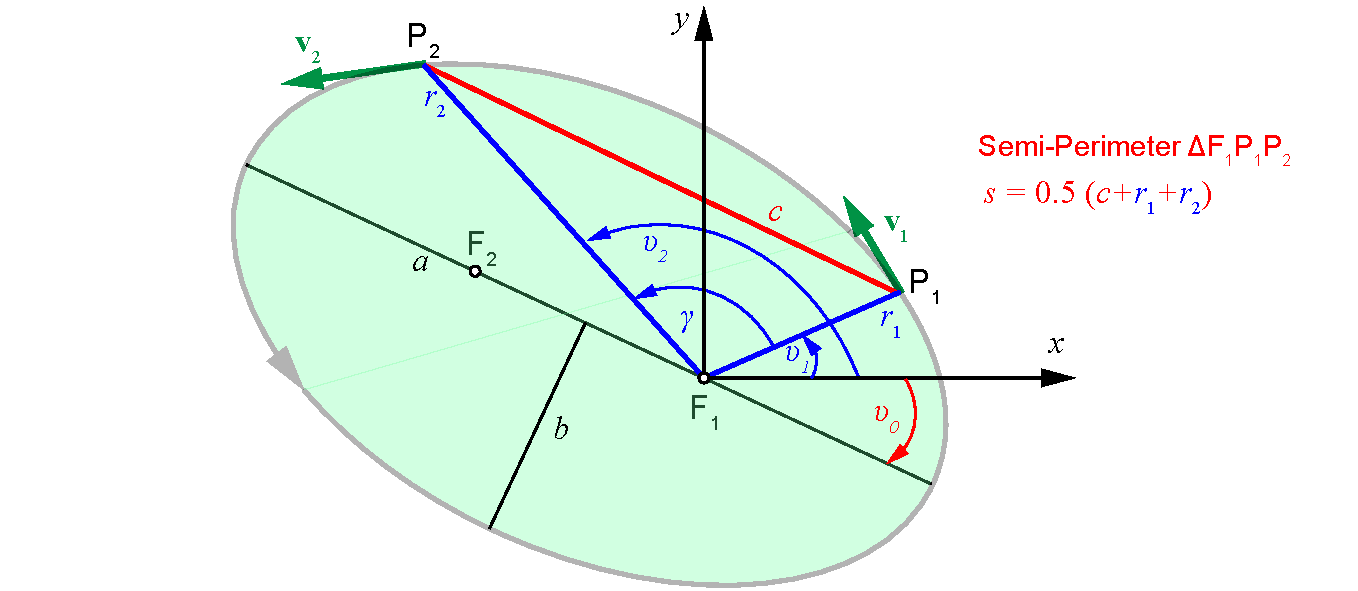
\includegraphics[width=\textwidth]{LambertProblem02Geometrie.pdf} 
	\caption[Geometrie des Lambert-Problems.]{Geometrie des Lambert-Problems.}
	\label{abb:adyn_lambert_lsg01}
\end{figure}

\medskip
%\hyperref[lsg:adyn_manoevers4]{\textcolor{blue} {$\rightarrow$ L�sungsvorschlag}}.\\
\linklsg\\%\href{FingerUeb2_AB.pdf#lsg:adyn_manoevers4}{\textcolor{blue} {$\rightarrow$ L�sungsteil}}.\\
\noindent\rule[1ex]{\textwidth}{0.5pt}
\end{prob}

%-----------------------------------------------------------------------------------------------------------
\begin{prob}  %�bung16
\schwierig{adyn_manoevers5}{Venus- und Mars-Fl�ge}
Benutzen Sie die L�sungsmethode des Lambert-Problems aus \probref{adyn_manoevers4}, um nun Venus- und Marsfl�ge aus einer Parkbahn um die Erde zu konzipieren. 
\begin{itemize}
	\item Berechnen Sie zun�chst die minimal m�gliche Transferzeit f�r ein gewisses Startdatum (\zb 18.6.2023). Diese wird durch einen parabolischen Orbit erreicht. \\
	\item Berechnen Sie nun f�r dieses Startdatum die Bahn f�r eine vorgegebene Flugzeit von 158 Tagen (zur Venus) \bzw 115 Tagen (zum Mars). \\
Benutzen Sie f�r Ihre Rechnungen die Werte aus der Tabelle \ref{tab:hm_bahnparameter} im Kapitel \ref{kap:hm_tabellen} der Himmelsmechanik. Hinweis: Sie k�nnen auch die Mittelpunktsgleichung\index{Mittelpunktsgleichung} \eqref{eq:hm_mpglg_r/a} aus \kap{hm_mpg} f�r eine einfache N�herung der elliptischen Bahnen von Mars und Venus verwenden.
\end{itemize}
Zusatzaufgabe: Suchen Sie ein optimales Startfenster f�r den Flug zum Mars aus. Wodurch ist dieses gekennzeichnet? Betrachten Sie dabei zwei F�lle:
	\begin{enumerate} [a)]
		\item Sie wollen nur einen Rover auf den Mars schaffen und zwar mit minimalen Treibstoffbedarf.
		\item Sie wollen mit Ihrer Crew auch m�glichst schnell wieder zur Erde zur�ck. Gehen Sie von realistischen Treibstoffvorr�ten aus. 
	\end{enumerate}

\medskip
%\hyperref[lsg:adyn_manoevers5]{\textcolor{blue} {$\rightarrow$ L�sungsvorschlag}}.\\
\linklsg\\%\href{FingerUeb2_AB.pdf#lsg:adyn_manoevers5}{\textcolor{blue} {$\rightarrow$ L�sungsteil}}.\\
\noindent\rule[1ex]{\textwidth}{0.5pt}
\end{prob}

%-----------------------------------------------------------------------------------------------------------
\begin{prob}  %�bung17
\mittel{adyn_manoevers6}{Abfang ballistischer Raketen}
Benutzen Sie die L�sungsmethode des Lambert-Problems aus \probref{adyn_manoevers4}, um ein Abfangman�ver zu berechnen.\\
Berechnen Sie das Geschwindigkeitsbudget, die Trajektorie und die Flugzeit einer Abfangrakete f�r eine interkontinentale ballistische Rakete (\textit{ICBM - \underline{I}nter-\underline{C}ontinental \underline{B}allistic \underline{M}issile}).\\
Die Abfangrakete befindet sich zum Zeitpunkt der Ortung bei:
\begin{align*}
	  \vec{r}(t_1)  = \vec{r}_1 = [6000, 3500, 0]\,\, \SI{}{\km}\,,~~~~
		\dot{\vec{r}}(t_1)  = \vec{v}_1 = [-2.5, 6.5, 2.5]\,\, \SI{}{\km\per\second}
\end{align*}
Die ICBM wurde getrackt mit:
\begin{align*}
	  \vec{R}(t_1)  &= \vec{R}_1 = [12250.0, 10250.0, 2000.0]\,\,\SI{}{\km}\,, ~~~~
		\dot{\vec{R}}(t_1) &= \vec{V}_1 = [-3.5, 1.0, 0] \,\,\SI{}{\km\per\second}
\end{align*}
Die ICBM soll binnen 30 min abgefangen werden und zwar bevor sie eine Flugh�he von 100 km erreicht. Ist das m�glich?
Zusatz: K�nnen Sie sagen, von wo die Rakete gestartet ist und wo sie ohne Abfang einschlagen w�rde?

\medskip
%\hyperref[lsg:adyn_manoevers6]{\textcolor{blue} {$\rightarrow$ L�sungsvorschlag}}.\\
\linklsg\\%\href{FingerUeb2_AB.pdf#lsg:adyn_manoevers6}{\textcolor{blue} {$\rightarrow$ L�sungsteil}}.\\
\noindent\rule[1ex]{\textwidth}{0.5pt}
\end{prob}


%-----------------------------------------------------------------------------------------------------------
\begin{prob}  %�bung18
\mittel{adyn_manoevers7}{Mondflug mit Ionenstrahltriebwerk}
L�sen Sie Bewegungsgleichung \eqref{eq:adyn_ionentr_01} numerisch f�r ein Triebwerk mit kontinuierlichem Schub f�r den Transfer aus einem LEO in einen GEO.\\
Parameter: $r_1= \SI{1000}{\km} + R_\text{E}$, $r_2 = \SI{35786}{\km} + R_\text{E}$, Schub $F_\text{S}= \SI{0.5}{\newton}$, Anfangsmasse $m_0= \SI{10000}{\kg}$, Massenaussto� $\dot{m}_\text{R} = \SI{3e-3}{\kg\per\second}$.\\

Berechnen Sie die Zeitdauer und Bahn f�r einen Mondflug mit einem Ionenstrahltriebwerk. Reduzieren Sie die Triebwerksleistung kontinuierlich so, dass diese bei einem Erreichen eines Abstands von der Erde, der dem Abstand des Lagrange-Punkts $\text{L}_1$ zwischen Erde und Mond entspricht, nahe Null wird. Vergleichen Sie mit dem Hohmann-Transfer.

\medskip
%\hyperref[lsg:adyn_manoevers7]{\textcolor{blue} {$\rightarrow$ L�sungsvorschlag}}.\\
\linklsg\\%\href{FingerUeb2_AB.pdf#lsg:adyn_manoevers7}{\textcolor{blue} {$\rightarrow$ L�sungsteil}}.\\
\noindent\rule[1ex]{\textwidth}{0.5pt}
\end{prob}

%-----------------------------------------------------------------------------------------------------------
\begin{prob}  %�bung19
\mittel{adyn_SOI}{Einflusssph�re - Sphere of Influence SOI}
Berechnen Sie die Radien der Einflusssph�ren der Planeten unseres Sonnensystems und vergleichen Sie mit dem Hill-Radius\index{Hill-Sph�re}, den wir in \probref{hm_hill_sphere} berechnet hatten. Worin unterscheiden sich die Radien? Wann muss man welchen heranziehen?

\medskip
%\hyperref[lsg:adyn_SOI]{\textcolor{blue} {$\rightarrow$ L�sungsvorschlag}}.\\
\linklsg\\%\href{FingerUeb2_AB.pdf#lsg:adyn_SOI}{\textcolor{blue} {$\rightarrow$ L�sungsteil}}.\\
\noindent\rule[1ex]{\textwidth}{0.5pt}
\end{prob}

%-----------------------------------------------------------------------------------------------------------

\begin{prob}  %�bung20
\mittel{adyn_swingby01}{Gravity-Assist-Man�ver - Analytische L�sung}
Finden Sie die analytischen L�sungen f�r $v_2$, $\Delta v = v_2 -v_1$ und $\gamma_2$ als Funktion der Eingangsparameter $v_1,\,v_\text{P},\,\gamma_1$. 
Finden Sie eine Beziehung f�r den Geschwindigkeits- und Energiegewinn beim Gravity-Assist-Man�ver und berechnen Sie die in der Tabelle \ref{tab:adyn_results_swingby}
in \kap{adyn_gravity_assist} angegebenen Werte f�r die theoretisch maximal erreichbaren Ablenkungen~$\vartheta'$ f�r die Planeten unseres Sonnensystems bei einem (unrealistischen) perizentralen Abstand von genau dem Planetenradius und einer typischen Einfluggeschwindigkeit von $v_1{}'= \SI{13.0}{\km\per\second}$. 

\medskip
%\hyperref[lsg:adyn_swingby01]{\textcolor{blue} {$\rightarrow$ L�sungsvorschlag}}.\\
\linklsg\\%\href{FingerUeb2_AB.pdf#lsg:adyn_swingby01}{\textcolor{blue} {$\rightarrow$ L�sungsteil}}.\\
\noindent\rule[1ex]{\textwidth}{0.5pt}
\end{prob}

%-----------------------------------------------------------------------------------------------------------

\begin{prob}  %�bung21
\einfach{adyn_swingby03}{Gravity-Assist-Man�ver - Simulation} 
Erstellen Sie in \matlab{} eine Simulation eines Gravity-Assist-Man�ver im Schwerefeld des Jupiters. \\

\medskip
%\hyperref[lsg:adyn_swingby03]{\textcolor{blue} {$\rightarrow$ L�sungsvorschlag}}.\\
\linklsg\\%\href{FingerUeb2_AB.pdf#lsg:adyn_swingby03}{\textcolor{blue} {$\rightarrow$ L�sungsteil}}.\\
\noindent\rule[1ex]{\textwidth}{0.5pt}
\end{prob}


%-----------------------------------------------------------------------------------------------------------

\newpage
\subsection{�bungen zu Rendezvous im Weltall}

\begin{prob}  %�bung22
\mittel{adyn_rendezvous01}{Rendezvous ISS und Raumtransporter}
Berechnen Sie, wie das Weltraum-Rendezvous zwischen der ISS und einem Raumtransporter stattfinden k�nnte. Ab welcher Entfernung kann die Bodenstation dem Kommandanten des Raumtransporters die Anweisung zur direkten manuellen Ansteuerung nach Sicht geben?

Gehen Sie von einer initial leicht elliptischen Bahn des Raumtransporters aus. Die gro�e Halbachse stimmt mit dem Radius der (nahezu) kreisf�rmigen Bahn der ISS �berein und die Exzentrizit�t betr�gt $e=0.035$. Beim Perig�um der Raumtransporterbahn haben die beiden Weltraumsysteme die gleiche wahre Anomalie.\\

Berechnen Sie auch numerisch f�r den Fall einer gro�er Elliptizit�t von $e=0.2$ die Bahnbeobachtung eines Raumschiffs von einer Raumstation aus der Kepler-L�sung, der L�sung aus der vollen Lagrange-Gleichung und zum Vergleich aus den CW-Gleichungen. Erkl�ren Sie Ihrer Ergebnisse.\\

\medskip
%\hyperref[lsg:adyn_rendezvous01]{\textcolor{blue} {$\rightarrow$ L�sungsvorschlag}}.\\
\linklsg\\%\href{FingerUeb2_AB.pdf#lsg:adyn_rendezvous01}{\textcolor{blue} {$\rightarrow$ L�sungsteil}}.\\
\noindent\rule[1ex]{\textwidth}{0.5pt}
\end{prob}
%-----------------------------------------------------------------------------------------------------------

\begin{prob}  %�bung23
\mittel{adyn_rendezvous02}{Rendezvous Apollo 11 CM und LM}
Berechnen Sie mit den Daten aus \kap{adyn_rendezvous_apollo11} und in der N�herung, dass die Bahnen von LM und CSM Kreisbahnen sind, wie das Weltraum-Rendezvous zwischen dem LM und dem CSM von Apollo 11 stattfand. Was k�nnen Sie �ber die Zeitabh�ngigkeit und die Genauigkeit des Zielwinkels des TPI-Burn sagen? 
Welcher Antriebsbedarf ist f�r den TPI-Burn notwendig? Ber�cksichtigen Sie dabei die Geschwindigkeit des LM vor dem TPI-Burn.\\
K�nnen Sie erkl�ren, warum der Astronaut Collins �ber die letzte Phase des "`geraden"' Anflugs etwas verwundert war?\\

\medskip
%\hyperref[lsg:adyn_rendezvous02]{\textcolor{blue} {$\rightarrow$ L�sungsvorschlag}}.\\
\linklsg\\%\href{FingerUeb2_AB.pdf#lsg:adyn_rendezvous02}{\textcolor{blue} {$\rightarrow$ L�sungsteil}}.\\
\noindent\rule[1ex]{\textwidth}{0.5pt}
\end{prob}

%-----------------------------------------------------------------------------------------------------------

\begin{prob}  %�bung24
\mittel{adyn_rendezvous03}{Planung einer Apollo Mission - \emph{Free Return Trajectory}}

Bei jeder der Apollo-Missionen zum Mond gab es eine besondere Sicherheitsma�nahme. F�r den Fall, dass die Mission aus irgendeinem Grund nicht so wie geplant durchgef�hrt werden konnte, wurde die Flugbahn des Apollo-Raumschiffs so geplant, dass es in einer freien R�ckflugbahn (\emph{Free Return Trajectory}) auf einer sogenannten \textit{slingshot trajectory} um den Mond herum "`geschleudert"' und nur durch die Gravitationskr�fte von Mond und Erde zur Erde zur�ckkehren w�rde. 
%In der Apollo 8 Mission wurde diese \textit{Free Return Trajectory} durch drei kurze Burns entsprechend angepasst.  Der erste Burn brachte Apollo 8 auf eine elliptische Umlaufbahn um den Mond, der zweite auf eine kreisf�rmige.  Apollo 8 umkreiste den Mond zehnmal und wurde dann nach einem dritten Burn wieder auf eine \textit{Free Return Trajectory} zur�ck zur Erde gebracht.  

Bei Apollo 13, der urspr�nglich dritten geplanten Mondlandemission, explodierte nach 56 Stunden Flugzeit ein Sauerstofftank an Bord des Raumschiffs. Das Raumschiff hatte nicht genug Treibstoff, um umzukehren und nach Hause zu fliegen. Es gab keine andere Wahl, als den Flug zum Mond fortzusetzen und auf der \textit{Free Return Trajectory} zur Erde zur�ckzukehren. Ohne die implizit eingebaute Sicherheitsma�nahme w�re das �berleben der Besatzung von Apollo 13 nicht m�glich gewesen.\\

Erstellen Sie zun�chst unter vereinfachenden Annahmen, dass  der Flug in der Mondbahnebene um die Erde stattfinden soll und dass nur die SOIs (\probref{adyn_SOI}) von Erde und Mond ber�cksichtigt werden sollen,  mittels der Methode des \textit{Patched-Conic-}N�herung\index{Patched-Conic-N�herung} (siehe \kap{adyn_gravity_assist}) 
eine erste n�herungsweise Missionsplanung f�r den Flug zum Mond. Bei der \textit{Free Return Trajectory} soll ohne weiteren Treibstoffverbrauch (von minimalen Kurskorrekturen abgesehen) nach der translunaren Injektion (\textit{Trans Lunar Injection} - TLI) eine sichere R�ckkehr zur Erde gew�hrleistet sein.\\
Versuchen Sie dann mit den so gewonnenen Anfangsdaten eine numerische L�sung.\\
Hinweise:
\begin{itemize}
	\item Beginnen Sie in der Erdumlaufbahn und legen Sie eine Richtung und eine Anfangsgeschwindigkeit f�r Ihre TLI fest.
	\item Stellen Sie die Trajektorie und die Position des Mondes dar.
	\item Zeigen Sie die Abh�ngigkeit der Flugbahn von Variationen in der Startgeschwindigkeit und der Startrichtung. 
\end{itemize}
Zusatz:
\begin{itemize}
	\item Berechnen Sie das n�tige Geschwindigkeitsbudget und die daf�r n�tige Treibstoffmenge f�r die TLI.
	\item Planen Sie eine Kurskorrektur, die das Raumschiff aus der \textit{Free Return Trajectory} in eine Mondumlaufbahn von ca. 120 km H�he bringt und eine weitere, die die Sonde aus dieser wieder in eine \textit{Free Return Trajectory} zur�ck zur Erde bringt.
\end{itemize}


F�r interessierte Leser sei auf das Apollo Flight Journal unter \url{https://www.nasa.gov/history/afj/} sowie die lesenswerte Beschreibung des Physikhintergrunds der Apollo-Missionen in \cite{Lundy2001} verwiesen, in denen jeweils alle Phasen der Apollo Missionen im Detail beschrieben sind.

\medskip
%\hyperref[lsg:adyn_rendezvous03]{\textcolor{blue} {$\rightarrow$ L�sungsvorschlag}}.\\
\linklsg\\%\href{FingerUeb2_AB.pdf#lsg:adyn_rendezvous03}{\textcolor{blue} {$\rightarrow$ L�sungsteil}}.\\
\noindent\rule[1ex]{\textwidth}{0.5pt}
\end{prob}

%-----------------------------------------------------------------------------------------------------------



\newpage
\subsection{�bungen zu Starts aus der Erdatmosph�re und zum Wiedereintritt}
%-----------------------------------------------------------------------------------------------------------

%\begin{prob}  %�bung25
%\einfach{adyn_forces01}{Kr�fte im Weltall}
%Berechnen Sie die Gr��enordnungen der Kr�fte von Tabelle \ref{tab:adyn_forces01}.
%�berlegen Sie sich die Wirkungen der Kr�fte auf die Umlaufbahnen von Satelliten.\\
%
%\medskip
%%\hyperref[lsg:adyn_forces01]{\textcolor{blue} {$\rightarrow$ L�sungsvorschlag}}.\\
%\linklsg\\%\href{FingerUeb2_AB.pdf#lsg:adyn_forces01}{\textcolor{blue} {$\rightarrow$ L�sungsteil}}.\\
%\noindent\rule[1ex]{\textwidth}{0.5pt}
%\end{prob}
%

%-----------------------------------------------------------------------------------------------------------

\begin{prob}  %�bung25
\mittel{adyn_launch01a}{Bewegungsgleichungen f�r Raketenstart von Erdoberfl�che}

Leiten Sie die skalaren Bewegungsgleichungen \eqref{eq:adyn_launch01} f�r einen Raketenstart von der Erdoberfl�che aus \eqref{eq:adyn_launch_vec} her.
Gehen Sie dabei von einem erdfesten \KOS\ in ein mitbewegtes \KOS\ �ber und schreiben Sie die Bewegungsgleichung in nat�rlichen Koordinaten und in geeigneten kartesischen Koordinaten ($h-x$).\\

\medskip
%\hyperref[lsg:adyn_launch01a]{\textcolor{blue} {$\rightarrow$ L�sungsvorschlag}}.\\
\linklsg\\%\href{FingerUeb2_AB.pdf#lsg:adyn_launch01a}{\textcolor{blue} {$\rightarrow$ L�sungsteil}}.\\
\noindent\rule[1ex]{\textwidth}{0.5pt}
\end{prob}


%-----------------------------------------------------------------------------------------------------------

\begin{prob}  %�bung26
\schwierig{adyn_launch01}{Raketenstarts von verschiedenen Weltraumzentren}
Die mathematisch-physikalische Behandlung eines Raketenstarts unter Ber�cksichtigung aller Faktoren (Atmosph�re, geographischer Ort der Startrampe, gew�nschte Bahn/Orbit, Nutzlast \usw) ist eine ziemlich komplexe Aufgabe, die letztendlich nur numerisch zu l�sen ist. Man kann mit den Erkenntnisse aus \kap{adyn_launch}
aber einige grunds�tzliche �berlegungen anstellen und Absch�tzungen machen, bevor man an die numerische Behandlung geht.\\
%Nach \figref{adyn_launch01} k�nnen wir den Flug eines Raumschiffs vom Start auf der Erdoberfl�che aus bis zum gew�nschten Orbit in 3 Phasen unterteilen:
%\begin{enumerate}
	%\item Schubphase
	%\item Freie Trajektorie (auch \textit{coasting phase} genant)
	%\item Gegebenenfalls eine Kurskorrektur (Burn) in den finalen, gew�nschten Orbit. 
%\end{enumerate}
In der �bung sollen folgende Aspekte behandelt werden:
\begin{itemize}
	\item Die Dynamik der Schubphase und den notwendigen Treibstoffbedarf  \bzw das Geschwindigkeitsbudget f�r das Erreichen eines bestimmten Orbits. Wir unterscheiden dabei den Fall des sogenannten \textit{Direct to Orbit} Transfers und des Transfers �ber eine Hohmann-Transferbahn mit anschlie�ender Kurskorrektur.
	\item Berechnung des Startverlaufs im mitbewegten \KOS{} nach \kap{adyn_launch} \bzw \probref{adyn_launch01a}.
	\item Festlegung des zeitlichen Startfensters und der Startrichtung (Startazimut) f�r den Start von verschiedenen Raumfahrtzentren im mitbewegten \KOS{} sowie im Inertialsystem.
	\item Komplette 3D-Trajektorienberechung der Startphase bis in den erdnahen Orbit.
\end{itemize}
Aufgabenstellungen:
\begin{enumerate}
\item Formulieren Sie eine allgemeine Optimierungsstrategie f�r einen Raumschiffstart in einen erdnahen Orbit. F�r die frei Trajektorie nehmen Sie einen Hohmann-Transfer an. Benutzen Sie auch die Ergebnisse von \kap{ady_reentry_conditions}. 
\item Berechnen Sie numerisch die Startphase einer dreistufigen Rakete (Ariane-1) im durch $\vec{t},\, \vec{n}$ und \vec{h} definierten mitbewegten \KOS. Ber�cksichtigen Sie den Drag und die Nickkorrektur. Legen Sie die Parameter so fest, dass die Rakete in eine Erdumlaufbahn von \ca 300 km H�he gelangt.
\item Zeigen Sie, dass man von einem Startort mit der geographischen Breite $\varphi_0$ ohne (treibstoffintensive) Bahnman�ver im Weltraum keine Orbits mit Inklinationen $i$ kleiner als $\varphi_0$ erreichen kann. Geben Sie auch eine physikalische Erkl�rung. Berechnen Sie f�r einen Raumschiffstart zur ISS jeweils Startfenster und Startazimut von Cape Canaveral, Baikonour und Kourou aus.
\item Berechnen Sie numerisch die 3D-Trajektorien im geozentrischen \KOS\ (Inertialsystem) f�r einen Raumschiffstart in eine Erdparkbahn von \ca 300 km jeweils von Cape Canaveral, Baikonour und Kourou aus. Ber�cksichtigen Sie den Einfluss der Erdrotation, der atmosph�rischen Reibung, ebenso wie den Nickwinkel und das Startazimut.
Berechnen Sie die Bodenspur des Raumschiffs von Start bis zum erstmaligen Abschluss einer Erdumrundung. 
Vergleichen Sie die Startbedingungen von den drei Zentren.\\
Benutzen Sie dabei die Daten aus Tabelle \ref{tab:adyn_parameter_raketen} f�r die Ariane-1 Rakete.
\end{enumerate}

\medskip
%\hyperref[lsg:adyn_launch01]{\textcolor{blue} {$\rightarrow$ L�sungsvorschlag}}.\\
\linklsg\\%\href{FingerUeb2_AB.pdf#lsg:adyn_launch01}{\textcolor{blue} {$\rightarrow$ L�sungsteil}}.\\
\noindent\rule[1ex]{\textwidth}{0.5pt}
\end{prob}

%-----------------------------------------------------------------------------------------------------------

\begin{prob}  %�bung27
\mittel{adyn_reentry01}{Parameter des Wiedereintritts in die Erdatmosph�re}
Leiten Sie die Beziehungen \eqref{eq:adyn_reentry03} mit den Kenntnissen aus \kap{hm_abl_kepler} her.\\
Vergleichen Sie die Problemstellung mit dem Lambert-Problem. Worin liegt der Unterschied, was gibt es f�r Gemeinsamkeiten?\\

\medskip
%\hyperref[lsg:adyn_reentry01]{\textcolor{blue} {$\rightarrow$ L�sungsvorschlag}}.\\
\linklsg\\%\href{FingerUeb2_AB.pdf#lsg:adyn_reentry01}{\textcolor{blue} {$\rightarrow$ L�sungsteil}}.\\
\noindent\rule[1ex]{\textwidth}{0.5pt}
\end{prob}

%-----------------------------------------------------------------------------------------------------------

\newpage
\begin{prob}  %�bung28
\mittel{adyn_reentry02}{Auftrieb/Drag-Abh�ngigkeit bei Wiedereintritt in Erdatmosph�re}
Untersuchen Sie die Abh�ngigkeit des H�henverlaufs $h(t)$. des Geschwindigkeitsverlaufs $v(t)$, des Flight Path Angle $\gamma(t)$ und der Beschleunigung (Abbremsung) $a(t)$ als Funktion des Verh�ltnisses von Auftrieb zu Drag f�r verschiedene initiale FPA.\\

\medskip
%\hyperref[lsg:adyn_reentry02]{\textcolor{blue} {$\rightarrow$ L�sungsvorschlag}}.\\
\linklsg\\%\href{FingerUeb2_AB.pdf#lsg:adyn_reentry02}{\textcolor{blue} {$\rightarrow$ L�sungsteil}}.\\
\noindent\rule[1ex]{\textwidth}{0.5pt}
\end{prob}

%-----------------------------------------------------------------------------------------------------------
\begin{prob}  %�bung29
\mittel{adyn_reentry03}{Normierte Gleichungen f�r $v(h)$ und $\gamma(h)$ bei Wiedereintritt}
Leiten Sie die Beziehung \eqref{eq:adyn_reentry11} aus \eqref{eq:adyn_launch08} f�r den Wiedereintritt in die Erdatmosph�re her.\\

\medskip
%\hyperref[lsg:adyn_reentry03]{\textcolor{blue} {$\rightarrow$ L�sungsvorschlag}}.\\
\linklsg\\%\href{FingerUeb2_AB.pdf#lsg:adyn_reentry03}{\textcolor{blue} {$\rightarrow$ L�sungsteil}}.\\
\noindent\rule[1ex]{\textwidth}{0.5pt}
\end{prob}

%-----------------------------------------------------------------------------------------------------------
\begin{prob}  %�bung30
\einfach{adyn_reentry04}{ISS Stabilit�t - Absturz und Vergl�hen des Satelliten Tiangong-1}
\begin{enumerate}
\item\textbf{\textit{Magnetsturm und ISS-Bahn}}\\
Dass ein Raumschiff beim Umkreisen der Erde wegen der minimal vorhandenen Reibung st�ndig an H�he verliert, ist v�llig normal. Bei der ISS sind es normalerweise \ca 100 Meter pro Tag. Berechnen Sie die mit einer geeigneten N�herungsrechnung die effektive Fl�che der ISS, die sich aus der normalen H�henverlustrate bei 420 km ergibt.
Wenn alle Systeme der ISS pl�tzlich ausfallen w�rden, wie lange w�rde es dauern, bis die ISS zum Absturz k�me?\\
W�hrend der heftigen Magnetst�rme im November 2004 sank die ISS bis zu 300 Meter pro Tag, so dass die Raumstation innerhalb weniger Tage um vier Kilometer an H�he verlor (\figref{adyn_ISS2004}).
Um wie viel gr��er war die Reibung durch den Magnetsturm im September? 

\begin{figure}[H]
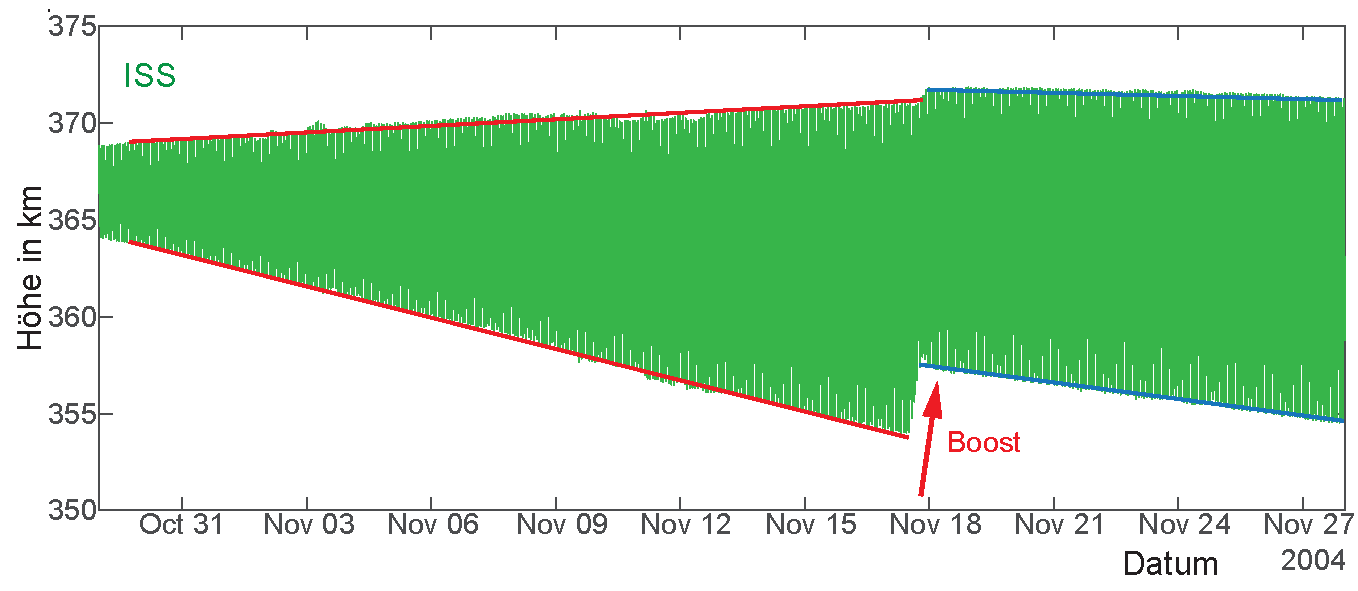
\includegraphics[width=\textwidth]{ISS2004.pdf}
\caption[H�he der Bahn der ISS im November 2004.]{H�henverlust der Bahn der ISS im November 2004 nach einem Magnetsturm. Daten von \cite{JPL2020}\, (siehe auch \mladyndref{ISS20004.txt}).}
\label{abb:adyn_ISS2004}
\end{figure}

\item \textbf{\textit{Der Absturz von Tiangong-1}}\\
Tiangong 1 (chinesisch f�r "`Himmelspalast 1"') war die erste Weltraumstation der Volksrepublik China. Der Start erfolgte mit einer Tr�gerrakete "`Langer Marsch"' am 29. September 2011. 
Das B�ro f�r bemannte Raumfahrt Chinas meldete am 21. M�rz 2016, dass die Ger�te an Bord von Tiangong-1 abgeschaltet wurden und dass sich seine Flugbahn im Laufe absenken und die Station in der Erdatmosph�re vergl�hen w�rde. Die Bahnh�he von Tiangong-1 verringerte sich zunehmend, der genaue Zeitpunkt des Wiedereintritts und damit der genaue Ort des Absturzes hing von der zum Teil unbekannten Dichte der Hochatmosph�re und von der Ausrichtung der Raumstation ab und lie� sich bis zuletzt nicht genau voraussagen.
Am 2. April 2018 um 00:16 Uhr UTC trat Tiangong-1 �ber dem S�dpazifik in die Erdatmosph�re ein und zerbrach in mehrere Teile (\figref{adyn_Tiangong2018}).
Untersuchen Sie mit einer geeigneten N�herungsrechnung den Absturz des Satelliten Tiangong-1 im Jahre 2018. Verwenden Sie die Daten aus \cite{JPL2020}\, (\mladyndref{Tiangong2018.csv}) \bzw \cite{Fiolhais2023, Pardini2019}.
\begin{figure}[H]
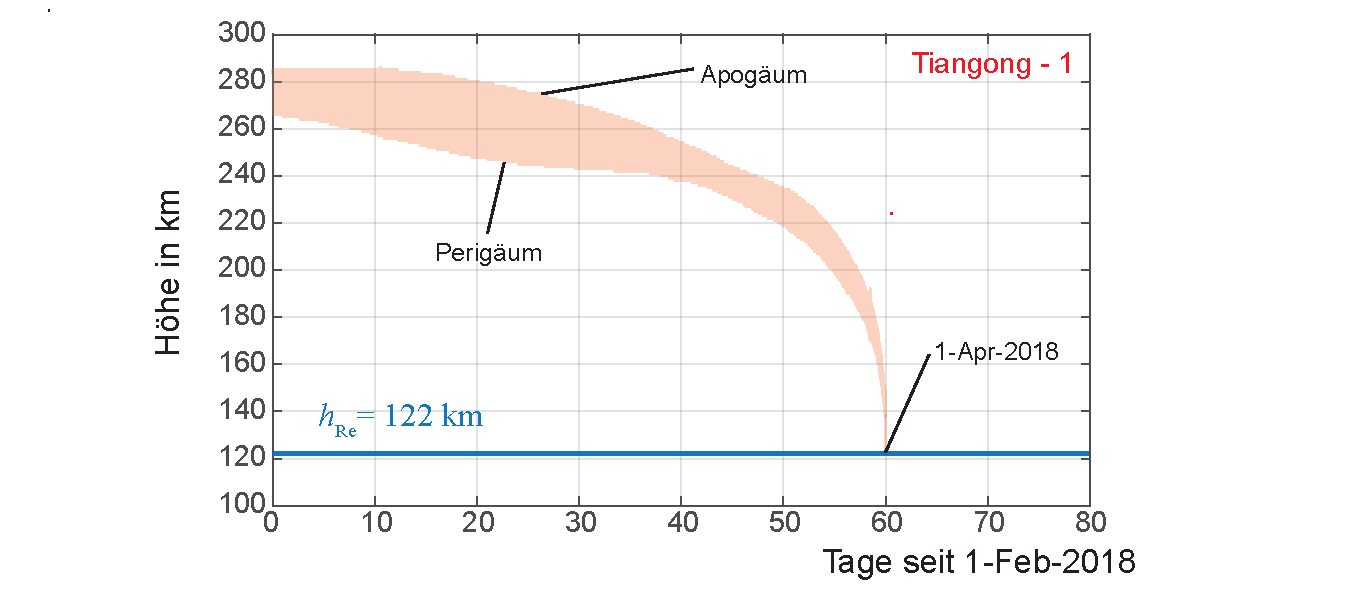
\includegraphics[width=0.95\textwidth]{Tiangong2018.pdf}
\caption[H�he der Bahn des chinesischen Satelliten Tiangong-1.]{H�he der Bahn des chinesischen Satelliten Tiangong-1 im Zeitraum Februar bis April 2018. Daten von \cite{JPL2020} (siehe auch \mladyndref{Tiangong2018.csv}).}
\label{abb:adyn_Tiangong2018}
\end{figure}

\item \textbf{\textit{Zusatzaufgabe 1}}\\

Berechnen Sie mit den Daten vom 05.03.2018 (\cite{JPL2020, Pardini2019} \bzw \mscr~\mladyndref{ISS2004.csv}) die Bahn der letzten Tage des Satelliten Tiangong-1 und die Bodenspur. Was ist Ihre Vorhersage? Vergleichen Sie mit dem tats�chlichen Ort des Vergl�hens (S�dpazifik $24.5\degree\,\text{S}, \, 151.1\degree\,\text{W}$).\\

\item \textbf{\textit{Zusatzaufgabe 2}}\\

Zeigen Sie numerisch wie extrem kritisch die Wiedereintrittsphase in einem solch einem Fall vom FPA $\gamma$ abh�ngt. Benutzen Sie die Ergebnisse von \probref{adyn_reentry03}.\\ 
\end{enumerate}

\medskip
%\hyperref[lsg:adyn_reentry04]{\textcolor{blue} {$\rightarrow$ L�sungsvorschlag}}.\\
\linklsg\\%\href{FingerUeb2_AB.pdf#lsg:adyn_reentry04}{\textcolor{blue} {$\rightarrow$ L�sungsteil}}.\\
\noindent\rule[1ex]{\textwidth}{0.5pt}
\end{prob}

%-----------------------------------------------------------------------------------------------------------
\begin{prob}  %�bung31
\einfach{adyn_BoatRocketModel}{Zur Entspannung}
Zum Abschluss zur Entspannung eine sch�ne Analogieaufgabe zwischen einer Rakete und einem Physiker als Bootsfahrer. Dieser will sich durch Abwerfen von Kokosn�ssen aus seinem Boot vorw�rts bewegen\footnote{Diese sch�ne Aufgabe geht auf \cite{Lagos2023} zur�ck}.\\
\figref{adyn_BoatRocketModel} zeigt die Situation des Bootsfahrers Leonardo, ohne Ruder und sonstigen Antrieb. Er hat lediglich $N$ Kokosn�sse der Masse $m_\text{K}$, die er jeweils mit einer Geschwindigkeit $v_\text{K}$ abwerfen kann. Sein Boot wiegt $m_\text{B}$, er selbst $m_\text{L}$. 
Zeigen Sie mit Hilfe des Impulserhaltungssatzes, dass das Problem �quivalent ist zu Raketengleichung und dass Sie f�r $N\rightarrow\infty$ und gleichzeitig  
$m_\text{K}\rightarrow 0$ tats�chlich die Raketengleichung erhalten.

\begin{figure}[H]
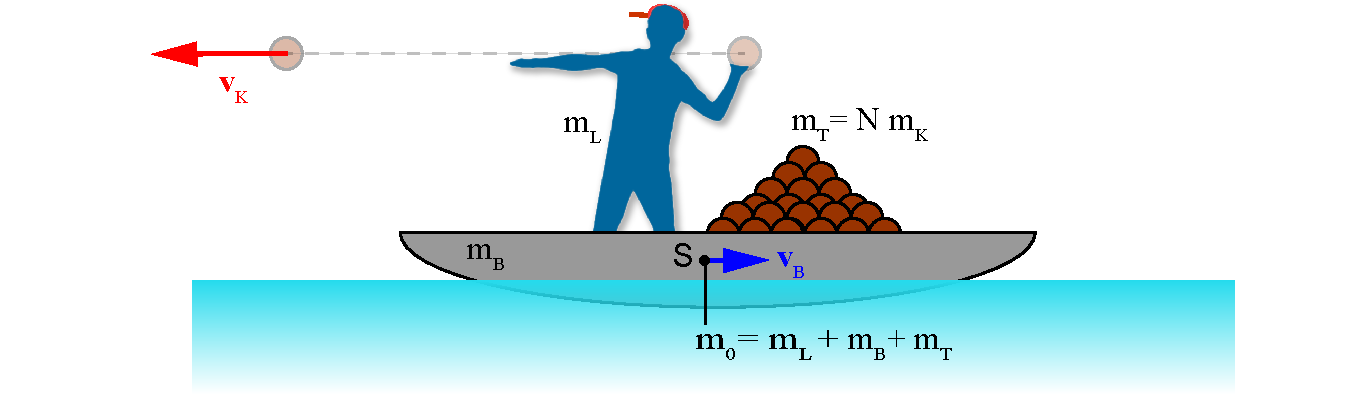
\includegraphics[width=\textwidth]{BoatRocketModel.pdf}
\caption[Diskretes Modell der Raketengleichung.]{Diskretes Modell der Raketengleichung.}
\label{abb:adyn_BoatRocketModel}
\end{figure}

\medskip
%\hyperref[lsg:adyn_BoatRocketModel]{\textcolor{blue} {$\rightarrow$ L�sungsvorschlag}}.\\
\linklsg\\%\href{FingerUeb2_AB.pdf#lsg:adyn_BoatRocketModel}{\textcolor{blue} {$\rightarrow$ L�sungsteil}}.\\
\noindent\rule[1ex]{\textwidth}{0.5pt}
\end{prob}


\newpage
\subsection{Weiterf�hrende Zusatzaufgaben und Probleme}

%-----------------------------------------------------------------------------------------------------------

\begin{prob}  %Zusatz1
\zusatz{adyn_launchinnovations}{Neue Ideen zum Flug ins Weltall}
Immer wieder gibt es Berichte zu alternativen und kosteng�nstigeren Methoden, Lasten von der Erde in den Weltraum zu bringen.
Besonders zwei Methoden haben in den letzten Jahren gro�e Aufmerksamkeit erreicht und auch entsprechendes Funding:
\begin{enumerate}
	\item Steinschleuder-Methode (englisch \textit{Spinlaunch}) \\
	Bei dieser relativ neuen, \ua von der Firma \textit{Spinlaunch} diskutierten Methode, wird mit einem rotierenden Massenbeschleuniger (einer Art Zentrifuge) eine geschossf�rmige Tr�gerrakete in gro�e H�hen katapultiert. Dort sollen die Triebwerke gez�ndet und die Nutzlast in eine Erdumlaufbahn gebracht werden. Dieses System soll weitaus kosteng�nstiger arbeiten als herk�mmliche Stufenraketen, ein erster Start wird f�r 2026 prognostiziert (\url{www.spinlaunch.com}, \cite{Krolle2022}).
	\item Weltraumfahrstuhl (englisch \textit{Space Elevator}) \\
	Die Idee dieser seit einigen Jahren \ua von der Firma \textit{Liftport} diskutierten Methode besteht darin, an einem Seil aus geeignetem Material Nutzlasten nach oben zu ziehen. Das Seil verl�uft vom �quator senkrecht nach oben �ber die geostation�re Bahn eines Satelliten hinaus und wird dort eventuell durch eine Gegenmasse abgeschlossen. (\url{www.liftport.com}, \cite{Aravind2007, Swan2013, Rauchhaupt2014}).
\end{enumerate}

Bewerten Sie diese Methoden, indem Sie einfache Absch�tzungen zur Realisierbarkeit machen. Was sind die Top-Probleme \bzw Herausforderungen. Welche Risiken sehen Sie?
K�nnen Sie eine Kostenabsch�tzung machen im Vergleich zu heutigen Kosten? SpaceX gibt heute $\SI{3000}{}$ USD pro kg Fracht an.\\
W�rden Sie investieren, in welches der beiden Projekte am ehesten?

\medskip
\linklsg\\%\hyperref[lsg:adyn_launchinnovations]{\textcolor{blue} {$\rightarrow$ L�sungsvorschlag}}.\\
\noindent\rule[1ex]{\textwidth}{0.5pt}
\end{prob}


%-----------------------------------------------------------------------------------------------------------

\begin{prob}  %Zusatz2
\zusatz{adyn_orbits_zusatz1}{Bahnparameter aus Bodenbeobachtungen (Ortsvektoren) }
Diese Aufgabe wurde aus \cite{Montenbruck2012} entnommen.\\
Berechnen Sie die Bahnparameter eines Satelliten f�r folgende Beobachtungen von der Station mit den geozentrischen Stationskoordinaten:\\
	$x_\text{B} = \SI{1344.143}{\km,}\,\, y_\text{B} = \SI{6068.601}{\km,}\,\,z_\text{B} = \SI{1429.311}{\km}\,.$  (Indien)\\
Die topozentrischen Messwerte f�r die indische Station sind:\\
	02.04.1999\,\, 00:30:00 UTC\,:\; $\mathcal{A} = 132.67\degree~\,,~h=32.44\degree~\,~  R_\text{S}=\SI{16945.45}{\km}$\,,\\
	02.04.1999\,\, 03:00:00 UTC\,:\; $\mathcal{A} = 123.08\degree~\,,~h=50.06\degree~\,~  R_\text{S}=\SI{37350.34}{\km}$\,.\\

\medskip
\linklsg\\%\hyperref[lsg:adyn_orbits_zusatz1]{\textcolor{blue} {$\rightarrow$ L�sungsvorschlag}}.\\
\noindent\rule[1ex]{\textwidth}{0.5pt}
\end{prob}

%-----------------------------------------------------------------------------------------------------------

\begin{prob}  %Zusatz3
\zusatz{adyn_orbits_zusatz2}{Bahnparameter aus Bodenbeobachtungen (Ortsvektoren) }
Berechnen Sie aus den in \probref{adyn_orbits3} berechneten topozentrischen Beobachtungsdaten zu den Zeiten 00:32 und 00:38 in G�rlitz nun umgekehrt die Bahnparameter.
Die Stationskoordinaten von G�rlitz sind: $\lambda = 15\degree$ O  und $\varphi=51\degree$ N.\\

\medskip
\linklsg\\%\hyperref[lsg:adyn_orbits_zusatz1]{\textcolor{blue} {$\rightarrow$ L�sungsvorschlag}}.\\
\noindent\rule[1ex]{\textwidth}{0.5pt}
\end{prob}



%-----------------------------------------------------------------------------------------------------------

\begin{prob}  %Zusatz4
\zusatz{adyn_manoevers8}{Marsflug mit Ionenstrahltriebwerk}
Konzipieren Sie einen Marsflug mit einem Ionenstrahltriebwerk. Seien Sie optimistisch und nehmen Sie eine Ausstr�mgeschwindigkeit von $v_\text{ion}=\SI{50}{\kilo\metre\per\second}$ und einen Anfangsschub von $\SI{50e-3}{\newton\per\kg}$ an. Das Raumschiff soll bereits in einer Parkbahn in 10000 km Abstand von der Mondoberfl�che kreisen. Welche Treibstoffmasse ist notwendig, was ist der gesamte Energiebedarf/Leistungsbedarf und mit welcher Flugzeit m�ssen Sie rechnen? Vergleichen Sie das mit einem Hohmann-Transfer \bzw der Flugzeit, die Sie in \probref{adyn_manoevers5} berechnet haben. \\
Was k�nnen Sie �ber das Nutzlastverh�ltnis sagen?\\
Hinweis: Gehen Sie analog zu \probref{adyn_manoevers7} vor und �berlegen Sie sich, welche sinnvollen N�herungen Sie f�r welchen Flugabschnitt machen k�nnen, um die numerische Rechnung zu vereinfachen und zu beschleunigen.

\medskip
%\hyperref[lsg:adyn_manoevers8]{\textcolor{blue} {$\rightarrow$ L�sungsvorschlag}}.\\
\noindent\rule[1ex]{\textwidth}{0.5pt}
\end{prob}


%-----------------------------------------------------------------------------------------------------------

\begin{prob}  %Zusatz5
\zusatz{adyn_swingby02}{Gravity-Assist-Man�ver - Allgemeiner Fall}
Betrachten Sie das GA-Man�ver im allgemeinen Fall, \dh dass die Bahnebene der Raumsonde und die Planetenebene nicht mehr �bereinstimmen (\figref{adyn_GA3dim}) und die
Bahnebene auch nicht mehr der Ekliptik entspricht. Geben Sie eine Berechnungsvorschrift f�r die Ausgangsparameter des GA-Man�vers in Matrixschreibweise an.
Finden Sie �ber eine vektorielle Definition des Streuparameters eine mathematische Formulierung f�r die jeweiligen F�lle des GA-Man�vers "`vor"' bzw. "`hinter"' einem Planeten und begr�nden Sie, warum sich daraus entweder $\vartheta' > 0$ oder $\vartheta' < 0$ ergibt.

\begin{figure}[H]
	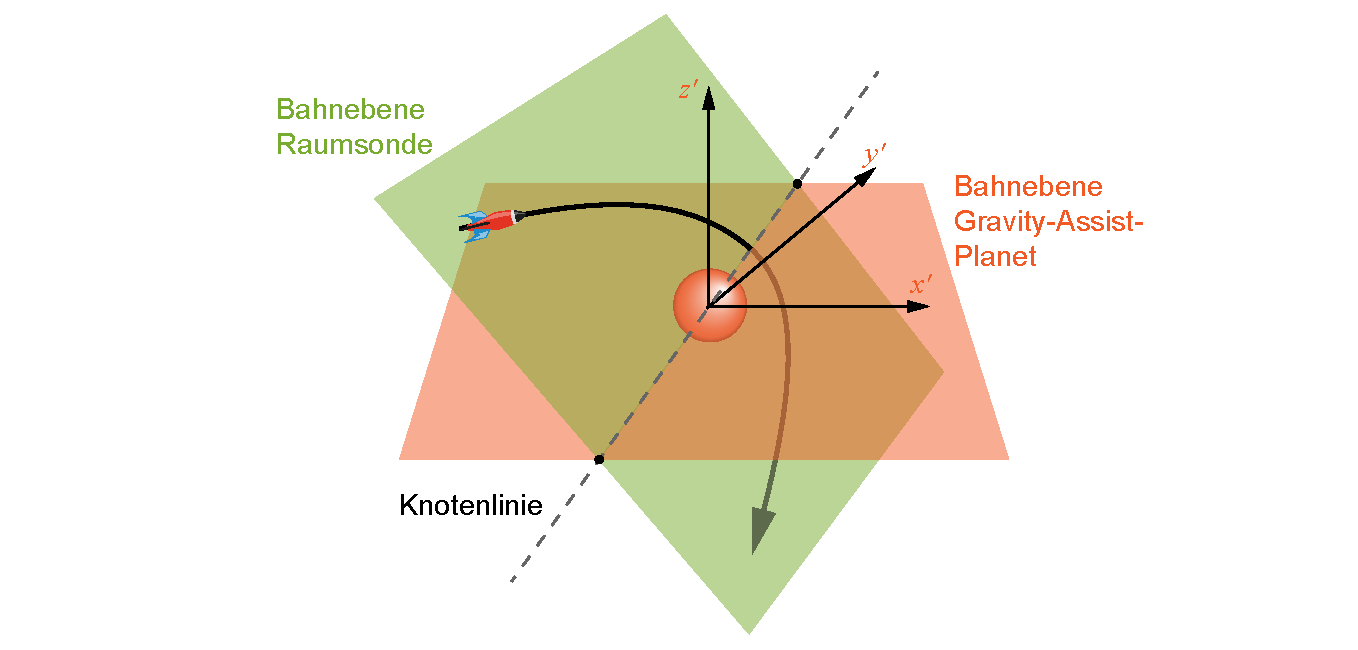
\includegraphics[width=\textwidth]{GravityAssist3D.pdf} 
	\caption[Geometrie des Gravity-Assist-Man�vers.]{Geometrie des Gravity-Assist-Man�vers (nichtkoplanarer Fall).}
	\label{abb:adyn_GA3dim}
\end{figure}
\medskip
\linklsg\\%\hyperref[lsg:adyn_swingby02]{\textcolor{blue} {$\rightarrow$ L�sungsvorschlag}}.\\
\noindent\rule[1ex]{\textwidth}{0.5pt}
\end{prob}


%-----------------------------------------------------------------------------------------------------------

\begin{prob}  %Zusatz6
\zusatz{adyn_swingby04}{Gravity-Assist-Man�ver - Zus�tzlicher Schub }
Berechnen Sie die Ausgangsparameter eines GA-Man�vers, bei dem die Raumsonde am Perizentrum noch einen Zusatzbetrag $\Delta v_\text{ext}$ aus den Treibstoffvorr�ten bekommt. Wie ver�ndern sich die Ausgangswerte zum Fall $\Delta v_\text{ext} = 0$ und zum Fall, wenn  $\Delta v_\text{ext}$ an den Punkten $\mathrm{P}_1$ \bzw  $\mathrm{P}_2$ zur Anwendung kommt. Diskutieren Sie Ihre Ergebnisse. 

\medskip
\linklsg\\%\hyperref[lsg:adyn_swingby04]{\textcolor{blue} {$\rightarrow$ L�sungsvorschlag}}.\\
\noindent\rule[1ex]{\textwidth}{0.5pt}
\end{prob}



%-----------------------------------------------------------------------------------------------------------

\begin{prob}  %Zusatz7
\zusatz{adyn_PSP01}{Flug der Parker Solar Probe - PSP}
Berechnen Sie die Bahn der PSP �ber die Patched-Conic-N�herung. Benutzen Sie dabei die Werte aus \kap{adyn_interplanetary_flights} und f�r die Anfangswerte der Bahn Daten der Horizon-Webseite des Jet Propulsion Lab \url{https://ssd.jpl.nasa.gov/horizons.cgi}. Die Daten sind  im File \mladyndref{PSP.csv} hinterlegt. F�r die Planeten k�nnen die Bahnen mit den Methoden aus dem \kap{hm_bahnen_hk_ss} in der Himmelsmechanik berechnet werden. \\
Ebenso sch�tze man ab, ob der Treibstoffvorrat dieser Sonde von $\SI{3650}{\kg}$ mit optimistischen  $v_\text{G} = \SI{4}{\km\per\second}$ ausgereicht h�tte, JUICE aus einer elliptischen Bahn um die Sonne (Perihelabstand von etwa $\SI{1}{AE}$) zum Jupiter zu bringen. Hinweis: Die gesamte mitgef�hrte Treibstoffmasse von JUICE betrug $\SI{3650}{\kg}$, die Strukturmasse und Nutzlast zusammen $\SI{2700}{\kg}$. Als Hinweis sei erw�hnt, dass die Startrakete eine Ariane 5 war, die f�r Transporte in den geostation�ren Orbit optimiert ist und die mit der Nutzlast von $\SI{6.3}{\tonne}$ beim Start voll ausgelastet war.

\medskip
%\hyperref[lsg:adyn_PSP01]{\textcolor{blue} {$\rightarrow$ L�sungsvorschlag}}.\\
\noindent\rule[1ex]{\textwidth}{0.5pt}
\end{prob}


%-----------------------------------------------------------------------------------------------------------

\begin{prob}  %Zusatz8
\zusatz{adyn_pertubations}{Gest�rte Satellitenbahnen - Grundideen der St�rungstheorie}
Berechnen Sie die �nderungen der Bahnparameter eines Satelliten (\bzw eines beliebigen Himmelsk�rpers) bei Vorhandensein einer beliebigen St�rkraft $\vec{F}_\text{S}$ zus�tzlich zum Zentralkraftfeld der Erde (\bzw des Zentralk�rpers) numerisch und durch analytische N�herungsformeln.
Benutzen Sie dabei das mit dem Satelliten mitbewegte Koordinatensystem~\vec{PQR}.

F�r die numerische Methode k�nnen Sie zwei verschiedene Methoden verwenden (vgl. auch \figref{adyn_pertubations01}):
\begin{enumerate}
	\item \textbf{Methode von Cowell}\footnote{Philip Herbert Cowell (1870 -- 1949) war ein britischer Astronom, der mit der nach ihm benannten Methode zur L�sung von Differentialgleichungen in rechtwinkligen Koordinaten einen bedeutenden Beitrag zur Berechnung der Bahnen von Himmelsk�rpern lieferte.}\indexp{Cowell, Philip Herbert}
	
	Die Cowell-Methode, Anfang des 20. Jahrhunderts ver�ffentlicht, besteht darin, dass man einfach die beiden Bewegungsgleichungen f�r die gest�rten Bahn $\vec{\rho}(t)$ und eine Referenzbahn $\vec{r}(t)$ (die sogenannte \gls{Oskulation}) \index{Bahn!oskulierende} \cite{Montenbruck1999} aufschreibt und diese dann simultan numerisch integriert.\\

	\item \textbf{Methode von Encke}\footnote{Johann Franz Encke (1791 -- 1865) war ein deutscher Astronom, der unter anderem die nach ihm benannte Enckesche Teilung des Saturnrings entdeckte. Er bestimmte die Bahnen vieler Kometen und Asteroiden mit hoher Genauigkeit, ebenso wie die Astronomische Einheit.}\indexp{Encke, Johann Franz}

	Die Encke-Methode, die bereits 1857 ver�ffentlicht wurde, besteht darin, dass man aus den beiden Bewegungsgleichungen f�r die gest�rten Bahn $\vec{\rho}(t)$ und die oskulierende Bahn $\vec{r}(t)$ eine Differentialgleichung f�r die Differenz $\vec{r}_\Delta (t)$ gewinnt und diese dann mit einem speziellen Verfahren numerisch integriert.
\end{enumerate}
	Beide Verfahren z�hlen zu den sogenannten speziellen St�rungstheorien, da letztendlich numerisch integriert werden muss.

	Alternativ kann man versuchen, analytisch �ber Reihenentwicklungen die zeitliche Variation der Bahnparameter aus den St�rbeschleunigungen abzuleiten. Dies ist erstmalig in einem ber�hmt gewordenen NASA-Report erfolgt \cite{NASA1968}. Man kann, dem dort dargelegten Prinzip folgend, f�r die Bahnparametervariationen $\D a/ \D t$, $\D e/ \D t$ \usw relativ kompakte Gleichungen herleiten und an diesen auch die Wirkung der unterschiedlichen St�rungen gut erkennen.
	
\begin{figure}[H]
	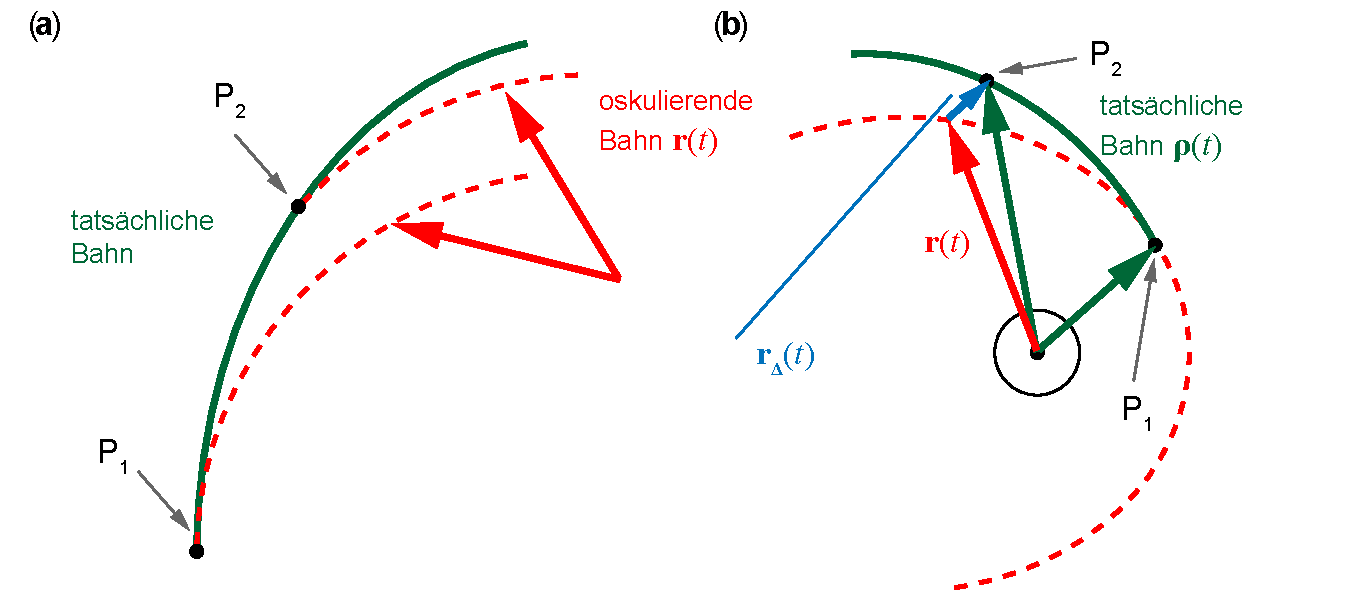
\includegraphics[width=\textwidth]{Stoerungsrechnung01.pdf} 
	\caption[Geometrie f�r die St�rungsrechnung.]{Geometrie f�r die St�rungsrechnung. \fa Definition der oskulierenden Bahn. \fb Definition von  $\vec{r}_\Delta (t)$ f�r die speziellen St�rungsrechnung nach der Methode von Encke.}
	\label{abb:adyn_pertubations01}
\end{figure}
\medskip
%\hyperref[lsg:adyn_PSP01]{\textcolor{blue} {$\rightarrow$ L�sungsvorschlag}}.\\
\noindent\rule[1ex]{\textwidth}{0.5pt}
\end{prob}

%-----------------------------------------------------------------------------------------------------------



 
%\clearpage
%\newpage
\subsection{\mscre -- Astrodynamik}\label{kap:adyn_matlabskripts}

Die \mscre befinden sich im MATLAB-Ordner \texttt{MatlabDateien/adyn},
die Hilfsfunktionen im dortigen Unterordner \texttt{Include\-folder} und Daten im Unterordner \texttt{Data}.
Es wird empfohlen, entweder die Skripte im GitHub Verzeichnis \githubSN zu benutzen oder sich die komplette Verzeichnisstruktur von \MKc~ runter zu laden und diese und auch das Arbeitsbuch im Hauptverzeichnis Fingeruebungen zu installieren. \\

Wir wollen noch einmal explizit darauf hinweisen, dass die \mscre prim�re der Vermittlung der physikalischen Modelle dienen und keinen Anspruch auf besonders elegante oder effiziente Programmierung erheben. Unser Buch ist ja kein Lehrbuch f�r \matlab-Programmierung. Uns ging es bewusst darum, dass die Skripte gut lesbar sind und das physikalische Modell bzw den physikalischen Gedankengang m�glichst klar abbilden.
Die Leser sind aufgerufen, die Programme nach Belieben zu verbessern und kompakter zu gestalten und diese auch ins GitHub Verzeichnis \githubSN zu stellen.

\subsubsection {Skripte zu Beispielen} \label{mls:adyn_kapitel} 
\begin{longtable}{p{0.34\textwidth}p{0.66\textwidth}}
\hline\noalign{\smallskip}
Skript & Beschreibung \\
\noalign{\smallskip}\svhline\noalign{\smallskip}
\mladynref{FlugzeitenMarsVenus.m}           & Programm berechnet die Flugzeiten f�r Hohmann-Ellipsen zu einem der Nachbar-Planeten (Venus, Mars) in der N�herung kreisf�rmiger Bahnen der Planeten.\\
\mladynref{GravityAssist01.m}               & Berechnet verschiedene Abh�ngigkeiten eines Gravity-Assist-Man�vers am Jupiter.\\
\mladynref{GravityAssist02.m}               & Berechnet verschiedene Abh�ngigkeiten der Gravity-Assist-Man�ver an den Planeten des Sonnensystems.\\
\mladynref{HohmannTransfer.m}               & Berechnet den Geschwindigkeitsbedarf f�r den Hohmann-Transfer als Funktion der Verh�ltnisse von Anfangs- und Endradius der kreisf�rmigen Erdumlaufbahnen von Satelliten und die Transferzeiten f�r interplanetare Hohman-Transfers.\\
\mladynref{Ionenantrieb01.m}                & Programm berechnet die Geschwindigkeitssch�be und die Bahnen/Flugzeiten f�r einen Ionenantrieb aus einem LEO in ein GEO im Vergleich zum Hohmann-Transfer (N�herungsl�sung).\\
\mladynref{LambertProblem01.m}              & Programm berechnet die Parameter der Ellipsenbahn f�r das Lambert-Problem �ber Iteration. Verwendet \mladyniref{LambertSolver1.m}\\
\mladynref{LambertProblem02.m}              & Programm berechnet die Parameter der Ellipsenbahn $a,\, e$ f�r das Lambert-Problem bei vorgegebener Geometrie f�r verschiedene ToF. Verwendet \mladyniref{LambertSolver2.m}\\
\mladynref{LambertProblem03.m}              & Programm berechnet die Parameter der Ellipsenbahn bzw. Hyperbelbahn f�r das allgemeine Lambert-Problem bei vorgegebenen Positionsvektoren 1 und 2 und der Richtung Bewegung, sowie der Flugzeit (ToF). Als Zentralk�rper ist entweder die Erde oder die Sonne angenommen. Verwendet \mladyniref{LambertSolver3.m}.\\
\mladynref{LMCSMApollo11.m}                 & Rendezvous von LM und CSM von Apollo 11 in der Mondumlaufbahn (Berechnung der Kinematik des Rendezvous �ber die Clohessy-Wiltshire-Gleichungen).\\
\mladynref{ParkerSolarProbe.m}              & Programm berechnet die einzelnen Gravity-Assist-Man�ver der Parker-Solar-Probe und simuliert die Bahn im Zeitraum von Start bis 2024.\\
\mladynref{Raketenstart01.m}                & Berechnet Start und Flug einer einstufigen Rakete von der Erdoberfl�che.\\
\mladynref{Raketenstart02.m}                & Programm berechnet Nutzlast-Antriebsverm�gen-Relation als Funktion des Strukturmassen-Verh�ltnisses.\\
\mladynref{Raketenstart03.m}                & Programm berechnet Nutzlast-Antriebsverm�gen-Relation f�r Ariane 1 und Saturn V.\\
\mladynref{RaketenstartReal.m}              & Programm berechnet Start einer einstufigen Rakete von der Erdoberfl�che unter Ber�cksichtigung von Reibung und Nickwinkel-Korrekturen.\\
\mladynref{ReentryNaeherungen.m}            & Programm berechnet die Dynamik des Wiedereintritts eines Raumschiffes in die Erdatmosph�re mit dem vollst�ndigen DGL-System in der N�herung $x,h \ll R_\text{E}$ und in den N�herungsl�sungen aus dem normierten DGL-System.\\
\mladynref{Rendezvous01.m}                  & Programm berechnet die Dynamik eines Weltall-Rendezvous eines Astronauten, der sich au�erhalb der Raumstation befindet mit der ISS. L�sung der Hill-Gleichungen und Clohessy-Wiltshire-Gleichungen (direkter Anflug mit verschiedenen Antriebsgeschwindigkeiten).\\
\mladynref{Rendezvous02.m}                  & Programm berechnet die Dynamik eines Weltall-Rendezvous eines Astronauten, der sich au�erhalb der Raumstation befindet mit der ISS. L�sung der Hill-Gleichungen und Clohessy-Wiltshire-Gleichungen (verschiedene Antriebsrichtungen).\\
\mladynref{Rendezvous03.m}                  & Berechnung der Kinematik eines Weltall-Rendezvous eines Targets und J�gers (L�sung �ber die Kepler-Gleichung bzw. die Clohessy-Wiltshire-Gleichungen).\\
\noalign{\smallskip}\svhline\noalign{\smallskip}
\end{longtable}

\subsubsection{Skripte zu �bungen} \label{mls:adyn_uebungen} %MLSkript�bungen
\begin{longtable}{p{0.34\textwidth}p{0.66\textwidth}}
\hline\noalign{\smallskip}
Skript & Beschreibung \\
\noalign{\smallskip}\svhline\noalign{\smallskip}
\mladynref{AlternativeRaketenGl.m}          & Berechnet die Raketengleichung nach einem diskreten Modell. \\
\mladynref{BahnparaBestimmung01.m}          & Berechnet die Bahnparameter von Satellitenbahnen um die Erde aus einem bekannten Orts- und Geschwindigkeitsvektor. \\
\mladynref{BiElliptischerTransfer.m}        & Berechnet Zwei-Impuls-�bergang von Bahn mit Radius $r_1$ auf eine elliptische Bahn (bielliptischer �bergang) mit Radius $r_2$.\\
\mladynref{FlugVenusParabelbahn.m}          & Programm berechnet die Parabel-Flugbahn einer Raumsonde zur Venus zu verschiedenen Startzeiten. Vorgegeben ist das Startdatum, gesucht ist das Ankunftsdatum mit dem schnellsten Transfer unabh�ngig vom notwendigen Antriebsbedarf.\\
\mladynref{FreReturTrajectorie01.m}         & Berechnet f�r verschiedene Parameter die Free Return Trajectorie um den Mond.\\
\mladynref{GravityAssistAnalytik.m}         & Analytische Formeln f�r Gravity-Assist-Man�ver und deren Auswertung.\\
\mladynref{GravityAssistSimulation.m}       & Programm simuliert die Streuung einer Raumsonde an einem Planeten (Gravity-Assist-Man�ver) im heliozentrischen KOS am Beispiel Jupiter.\\
\mladynref{IonenantriebMond.m}              & Programm berechnet die Geschwindigkeitssch�be und die Bahnen/Flugzeiten f�r einen Ionenantrieb aus einem LEO zum Mond im Vergleich zum Hohmann-Transfer.\\
\mladynref{Ionenantrieb02.m}                & Programm berechnet die Geschwindigkeitssch�be und die Bahnen/Flugzeiten f�r einen Ionenantrieb aus einem LEO in ein GEO im Vergleich zum Hohmann-Transfer.\\
\mladynref{LambertICBM.m}                   & Programm berechnet die Parameter des Abfangens einer ICBM  (Intercontinental Ballistic Missile) �ber die L�sung (Bisektionsverfahren) des Lambert-Problems. Verwendet \mladynref{LambertSolver3.m}.\\
\mladynref{LambertMarsVenus.m}              & Programm berechnet die Parameter der Ellipsenbahn f�r Fl�ge zu Mars und Venus f�r das Lambert-Problem bei vorgegebenen Positionsvektoren 1 und 2 in AE, sowie der Abflug und Ankunftszeit. Verwendet \mladynref{LambertSolver3.m}.\\
%\mladynref{LambertSolver3.m}                &.\\
\mladynref{OberthEffektAnalogie.m}          & Analogie zum Oberth-Effekt als Bewegung durch eine Potentialmulde.\\
\mladynref{OberthSwingBy.m}                 & Berechnet Swing-By Man�ver mit Oberth-Effekt am Beispiel Jupiter.\\
\mladynref{RaketenOptimierung01.m}          & Optimierung einer Mehrstufenrakete (Tandemstufung).\\
\mladynref{RaketenOptimierung02.m}          & Optimierung einer Mehrstufenrakete mit der Methode der Lagrange-Multiplikatoren am Beispiel Saturn V und Apollo~11.\\
\mladynref{Raketen2Orbit01.m}               & Programm berechnet Start einer zweistufigen Rakete von der Erdoberfl�che unter Ber�cksichtigung von Reibung und Nickwinkel-Korrekturen. Berechnung im mitbewegten KOS.\\
\mladynref{Raketen2Orbit02.m}               & Programm berechnet Start einer dreistufigen Rakete von der Erdoberfl�che unter Ber�cksichtigung von Reibung und Nickwinkel-Korrekturen. Berechnung im mitbewegten KOS.\\
\mladynref{Raketen2Orbit03.m}               & Programm berechnet Startazimut und Startfenster f�r Start eines Raumschiffs zur ISS von verschiedenen Weltraumzentren.\\
\mladynref{Raketenstart04.m}                & Programm berechnet Nutzlast-Antriebsverm�gen-Relation f�r gleiche Struktur-/Treibstoffmassenverh�ltnisse als Funktion der Stufenzahl $N$.\\
\mladynref{ReentryReal.m}                   & Programm berechnet die Dynamik des Wiedereintritts (Reentry) eines Raumschiffes in die Erdatmosph�re f�r verschiedene Eintrittswinkel $\gamma_\text{Re}$ und Auftrieb-Drag-Relationen.\\
\mladynref{ReentrySummary.m}                & Programm berechnet die Dynamik des Wiedereintritts (Reentry) eines Raumschiffes in die Erdatmosph�re f�r verschiedene Eintrittswinkel $\gamma_\text{Re}$.\\
\mladynref{Rendezvous04.m}                  & Berechnung der Kinematik eines Weltall-Rendezvous eines Raumtransporters und der ISS (L�sung �ber die Kepler-Gleichung bzw. Clohessy-Wiltshire-Gleichungen) und Anflug mit direkter Sichtlinie.\\
\mladynref{Rendezvous05.m}                  & Berechnung der Kinematik eines Weltall-Rendezvous eines Raumtransporters und der ISS (L�sung �ber die vollst�ndige Lagrange-Gleichung im Vergleich zur L�sung Clohessy-Wiltshire-Gleichungen).\\
\mladynref{SatPositionen01.m}               & Programm berechnet die Positionen und Bodenspuren von verschiedenen Satelliten um die Erde �ber die L�sung der Kepler-Gleichung.\\
\mladynref{SatPositionen02.m}               & Programm berechnet die Bahnparameter und die Bodenspur der ISS auf Basis von Daten der NASA. \\
\mladynref{SatPositionen03.m}               & Bestimmung der topozentrischen Beobachtungsdaten eines polaren Satelliten und der ISS.\\
\mladynref{SatPositionen04.m}               & Bestimmung der Bodenspur der ISS und ihrer topozentrischer Beobachtungsdaten von zwei Bodenstationen aus. \\
\mladynref{SatPositionen05.m}               & Bestimmung der topozentrische Beobachtungsdaten eines polaren Satelliten von zwei Bodenstationen aus\\
\mladynref{SonnenSynchroneBahn.m}           & Berechnung der Bahn und der Bodenspur eines sonnensynchronen Satelliten.\\
\mladynref{Spinlaunch.m}                    & Simulation eines Raketenstarts mit dem Spinlaunch System.\\
\mladynref{Transfer2Moon.m}                 & Berechnet verschiedene Parameter und Trajektorien f�r einen Flug zum Mond.\\
\mladynref{Transfer2MoonExample.m}          & Berechnet verschiedene Parameter und Trajektorien f�r einen Flug zum Mond. Parameter $r_0, v_0, \gamma_0, \lambda_1$ werden vorgegeben.\\
\mladynref{FreReturTrajectorie01.m}         & Berechnet f�r verschiedene Parameter die Free Return Trajectorie um den Mond.\\
\mladynref{TransferUnendlich.m}             & Programm berechnet die Geschwindigkeitsbedarfe f�r Hohmann-Oberth-Edelbaum-Transfers nach Unendlich, ebenso wie die Flugzeiten (normiert auf die Anfangsgeschwindigkeit/Umlaufzeit/Radius der Anfangs-Kreisbahn).\\
\mladynref{Transfer2Reentry.m}              & Programm berechnet die Transferbahnparameter (Deorbit) aus einer Kreisbahn zum Wiedereintritts (Reentry) eines Raumschiffes in die Erdatmosph�re in Abh�ngigkeit vom Eintrittswinkel $\gamma_\text{Re}$.\\


\noalign{\smallskip}\hline\noalign{\smallskip}
\end{longtable}

\subsubsection {Hilfsfunktionen} \label{mls:adyn_hilfsfunktionen} 

\begin{longtable}{p{0.33\textwidth}p{0.67\textwidth}}
\hline\noalign{\smallskip}
Skript & Beschreibung \\
\noalign{\smallskip}\svhline\noalign{\smallskip}
\mladyniref{EulerLagrange.m}             & Symbolische Berechnung der Euler-Lagrange Gleichungen (\url{https://www.mathworks.com/matlabcentral/fileexchange/93275-euler-lagrange-solver}), MATLAB Central File Exchange. 27.12.2021, Copyright (c)  Morten Veng 2021.\\
\mladyniref{R\_x.m} , \mladyniref{R\_y.m}, \mladyniref{R\_z.m}     & Rotationsmatrizen bez�glich x,y,z-Achse.\\
\mladyniref{LambertSolver1.m}            & Routine zur Berechnung des Bahnparameters $p, e$ der Ellipsenbahn f�r das Lambert Problem durch ein Bisektionsverfahren.\\
\mladyniref{LambertSolver2.m}            & Routine zur Berechnung des Bahnparameters $a, e$ der Ellipsenbahn f�r das Lambert Problem durch ein Bisektionsverfahren.\\
\mladyniref{LambertSolver3.m}            & Allgemeine Routine zur Berechnung der Bahnparameters $a, e$ der Ellipsen- \bzw Hyperbelbahn f�r das Lambert Problem auf Basis der Methode von Battin \cite{Battin1999}. Copyright (c) 2017, Meysam Mahooti.\\
\mladyniref{GetColorLines.m}             & L�dt Farbtabelle f�r Linien und graphische Darstellungen.\\
\noalign{\smallskip}\svhline\noalign{\smallskip}
\end{longtable}

 
%\clearpage
%\section{L�sungsbeispiele \autoref{chap:adyn} -- Astrodynamik}\label{chap:adyn_lsguebungen}

Die in den L�sungsvorschl�gen angegebenen \mscre finden sich im GitHub unter \githubSN \bzw
in den \onlineZ{} (\MKc).\\
Sie sind wirklich als Vorschlag f�r eine m�gliche L�sung gedacht, wohl wissend, dass es in der Physik oft ganz verschiedene, manchmal auch elegantere als die hier vorgestellten L�sungen gibt, um ein Problem zu l�sen. Das macht ja gerade den Reiz der Physik aus.
Wir laden die Leser ein, ihre L�sungen auch unter \githubSN \bzw auf den online-Seiten (\MKc) zu teilen.
Wir sind in jedem Fall gespannt.

%%-----------------------------------------------------------------------------------------------------------

\subsection{�bungen zu Grundlagen der Raketenphysik}

\medskip

-----------------------------------------------------------------------------------------------------------

\begin{sol}{prob:adyn_canonball}\label{lsg:adyn_canonball} %�bung1
\textbf{Jules Vernes Kanonenschuss zum Mond}\\

Wir wissen, dass ein Objekt, das zum Mond fliegen soll, eine bestimmte kinetische Energie braucht, um das Gravitationsfeld der Erde zu verlassen:
\begin{align*}
    \frac{m}{2}\,v^2 = G\,\frac{m_\text{E}\,m}{R_\text{E}}\,,
\end{align*}
woraus die 2.\,\gls{vkosmos} oder auch \gls{vescape} 
$v_\text{F} = \sqrt{2\,G\,m_\text{E}/R_\text{E}} \approx \SI{11.2}{\km\per\second}$
folgt. Das \textit{Problem Nr. 1} ist das Erreichen dieser Fluchtgeschwindigkeit. Im Buch gibt Verne eine Masse der Kapsel von \ca $m_\text{R} = \SI{8.75}{\tonne}$ und eine Sprengstoffmasse von Schie�baumwolle $m_\text{SB}$ von \ca $\SI{182}{\tonne}$ an. Schie�baumwolle (auch Nitrozellulose genannt) wurde 1846 entdeckt und hat eine f�r das Projekt \textit{Columbiade} relevante Detonationsgeschwindigkeit von $\SI{6300}{\metre\per\second}$ \bzw eine spezifische Explosionsenergie von $\epsilon = \SI{5475}{\kilo\J\per\kg}$.
Wir k�nnen den Energieerhaltungssatz aufschreiben und nehmen an, dass das Gas und die Kapsel an der Kanonenrohr�ffnung beim Verlassen dieser die gleiche Geschwindigkeit haben:
\begin{align*}
    \epsilon\,m_\text{SB}\,&= \frac{m_\text{SB}}{2}\,v^2 + \frac{m_\text{R}}{2}\,v^2  ~~~~ \rightarrow ~~~ v = \sqrt{\frac{2\,m_\text{SB}\,\epsilon}{m_\text{SB}+m_\text{R}}} = \SI{3232}{\metre\per\second}\,.
\end{align*}
Das ist deutlich geringer als die notwendigen $v_\text{F} = \SI{11.2}{\km\per\second}$. 
Das \textit{Problem Nr. 2} ist aber noch ein anderes: Selbst wenn es einen Sprengstoff g�be, der eine Geschwindigkeit von gr��er $\SI{11.2}{\km\per\second}$ an der Rohrm�ndung erlauben w�rde, m�sste auf der L�nge des Rohrs (nach Verne $s = \SI{270}{\metre}$) eine Beschleunigung von
\begin{align*}
    a = \frac{v_\text{F}{}^2}{2s} \approx \SI{2.32e5}{\metre\per\square\second} \approx \SI{23700}{}\, g
\end{align*}
wirken. Wenn man wei�, dass man bereits bei einer Belastung von $\SI{10}{}\,g$ in Ohnmacht fallen kann, wird es nicht viele Freiwillige gegeben haben. \\
Man k�nnte nat�rlich die Beschleunigungsstrecke l�nger machen, so dass nur $\SI{10}{}\,g$ auf die Astronauten wirken. Dann m�sste das Kanonenrohr aber 
$s = v_\text{F}{}^2/(\SI{20}{}\,g) \approx \SI{640}{\km}$ lang sein. %was l�nger ist als die Strecken M�nchen-Hamburg (612\,km) bzw. Baltimore-Boston (578 km).\\
\end{sol} 
\textcolor{blue} {$\rightarrow$ zur} \probref{adyn_canonball}.\\
\noindent\rule[1ex]{\textwidth}{0.5pt}  \newpage  \clearpage

%-----------------------------------------------------------------------------------------------------------

\begin{sol}{prob:adyn_rocketbasic}\label{lsg:adyn_rocketbasic} %�bung2
\textbf{Prinzip Mehrstufenrakete}\\ \\
Wir starten von \eqref{eq:adyn_rockets19} und zeigen zun�chst, dass f�r eine einstufige Rakete diese Gleichung in die Ziolkowski-Gleichung �bergeht ($N=i=1$)
\begin{align*}
    \Delta v_\text{ges} = v_\text{G}\,\ln\,\frac{m_1}{\sigma_1\,m_1+m_\text{L}} = v_\text{G}\,\ln\,\frac{1}{\sigma_1 + m_\text{L}/m_1}\,.
\end{align*}
Mit $\sigma_1\approx 0$ folgt daraus die Ziolkowski-Gleichung $\Delta v = v_\text{G}\,\ln(m_1/m_\text{L})$.\\
Wir setzen nun in \eqref{eq:adyn_rockets19} alle $v_{\text{G},i}= v_\text{G}{}^*$ und benutzen ebenfalls:
	\[\mathcal{M}^* = \frac{m_{0,i}}{m_{0,i}-m_{\text{T},i}}\,.	\]
\begin{align*}
    \Delta v = v_\text{G}^*\,\sum\limits_{i=1}^N\ln\,\frac{m_{0,i}}{\sigma_i\,m_{0,i} + m_{0,i+1}}\,.
\end{align*}
Nun war ja $\sigma_i$ definiert als \eqref{eq:adyn_rockets18}:
\begin{align*}
    \sigma_i = \frac{m_{0,i}- m_{\text{T},i}- m_{0,i+1}}{m_{0,i}}\,,
\end{align*}
womit wir erhalten:
\begin{align}
    \Delta v &= v_\text{G}^* \,\sum_{i=1}^N\ln\,\frac{m_{0,i}}{m_{0,i} - m_{\text{T},i} - \killA{m_{0,i+1}} + \killA{m_{0,i+1}}}\nonumber \\
             &= v_\text{G}^* \,\sum_{i=1}^N\ln\,\frac{m_{0,i}}{m_{0,i} - m_{\text{T},i} } =  v_\text{G}^* \,\sum_{i=1}^N\ln\,\mathcal{M}^* =  v_\text{G}^* \,N\,\ln \,\mathcal{M}^*\,. 
						\label{eq:adyn_lsg_rocket01}
\end{align}
Damit haben wir die erste Gleichung von \eqref{eq:adyn_rockets20} bewiesen. \\
Das Nutzlastverh�ltnis ist gegeben durch:
\begin{align*}
    \mu_\text{L}= \frac{m_\text{L}}{m_0} = \frac{m_\text{L}}{\sum\limits_{i=1}^N m_i+m_\text{L}}\,.
\end{align*}
Die Strukturmassen wollen wir gegen�ber den Treibstoffmassen vernachl�ssigen, so dass mit $\lk\mathcal{M}^*\rk^N$ und mit der Masse der $i$-ten Unterrakete
	\[ 
	m_{0,i} = \lk \sum\limits_{j=i}^N m_{\text{T},j} \rk + m_\text{L}  \approx m_{0,i-1} + m_{\text{T},i} 
	\]
(siehe auch \figref{adyn_rockets04}a gilt:
\begin{align*}
     \lk \mathcal{M}^* \rk ^N  &= \lk \frac{m_{0,i}}{m_{0,i}-m_{\text{T},i}}\rk^N \approx \frac{m_0}{ \lk \sum\limits_{i=2}^N m_{\text{T},i} \rk + m_\text{L}}\, \dot\,\frac{ \lk \sum\limits_{i=2}^N m_{\text{T},i} \rk + m_\text{L}}{\lk \sum\limits_{i=3}^N m_{\text{T},i} \rk + m_\text{L}}\,\dot\,\ldots \,\dot\, \frac{\lk \sum\limits_{i=N-1}^N m_{\text{T},i} \rk + m_\text{L}}{m_\text{L}}\,\approx\, \frac{m_0}{m_\text{L}}\,,
\end{align*}
woraus die zweite Gleichung von \eqref{eq:adyn_rockets20} 
\begin{align}
    \frac{m_\text{L}}{m_0} \approx \lk \mathcal{M}^*\rk^{-N}\, \label{eq:adyn_lsg_rocket02}
\end{align}
folgt.

\begin{figure}[H]
	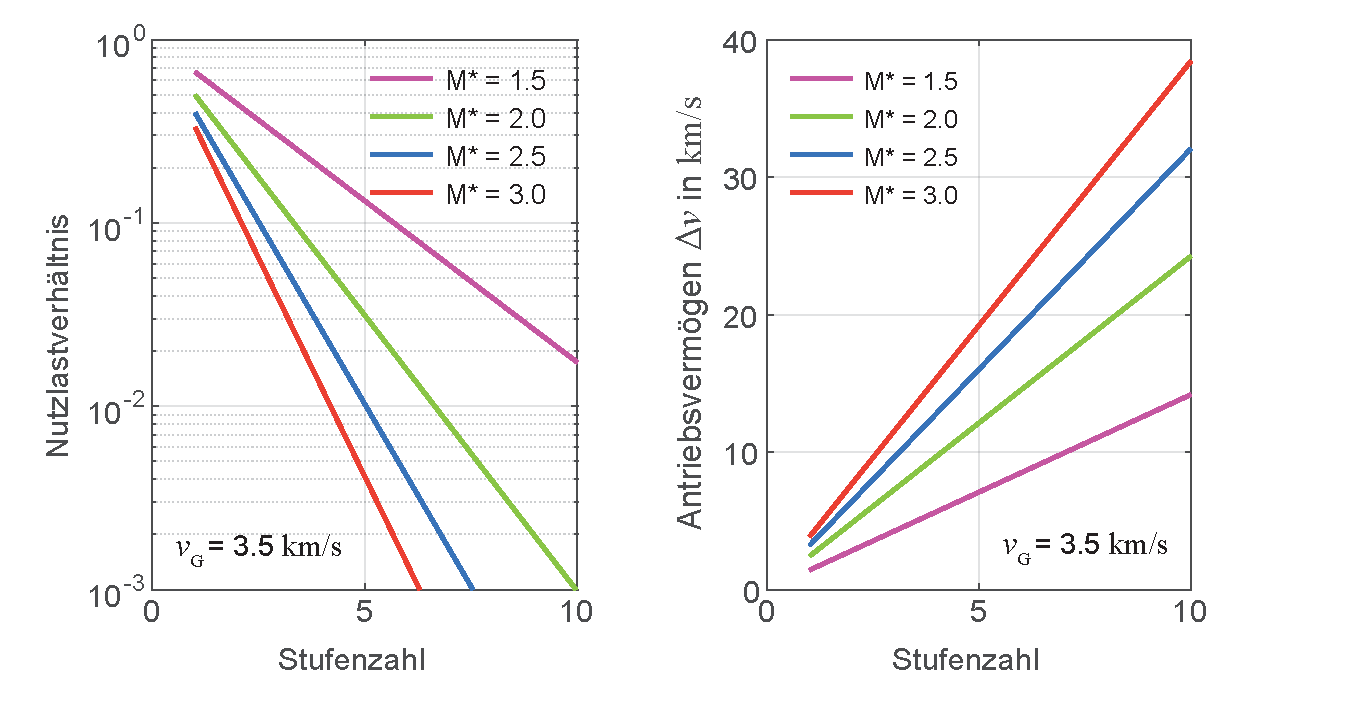
\includegraphics[width=\textwidth]{MehrStufenTheorie.pdf} 
	\caption[Nutzlastverh�ltnis �ber Antriebsbudget f�r mehrstufige Raketen.]{Nutzlastverh�ltnis �ber Antriebsbudget f�r mehrstufige Raketen bei gleichen $v_{\text{G},i}= v_\text{G}{}^*$ und 
	gleichen Struktur- und Treibstoffmassen aller Unterraketen ($\mathcal{M}^* = m_{0,i}/(m_{0,i}-m_{\text{T},i})$). Siehe \matlab{}-Datei
\mladynref{Raketenstart04.m}.}
	\label{abb:adyn_rocket_lsg05}
\end{figure}

\end{sol} 
\textcolor{blue} {$\rightarrow$ zur} \probref{adyn_rocketbasic}.\\
\noindent\rule[1ex]{\textwidth}{0.5pt}  \newpage  \clearpage

%-----------------------------------------------------------------------------------------------------------


\begin{sol}{prob:adyn_rocketopt1}\label{lsg:adyn_rocketopt1} %�bung3
\textbf{Optimierung Mehrstufenrakete (Tandemstufung)}\\
\begin{enumerate}
	\item \textit{\textbf{L�sungsansatz �ber Extremwertberechnung - Beispiel Saturn V Maximalleistung 100 t Nutzlast}}\\ 
Wir starten von der Raketen-Gleichung f�r die Tandemstufung \eqref{eq:adyn_rockets19} und fordern, dass f�r ein Nutzlastverh�ltnis
\begin{align}
    \Delta v = \sum\limits_{i_1}^N \Delta v_i = \sum\limits_{i_1}^N v_{\text{G},i}\,\ln\,\frac{1}{\sigma_i + \frac{\mu_{i+1}}{\mu_i}}\,.\label{eq:adyn_rocketsopt01} ~~~~ \rightarrow ~~~~ \text{max}
\end{align}
gelten soll. Die Bedingung f�r das Maximum lautet, wenn $\mu_\text{L}$ und alle $\sigma_i$ gegeben sind:
\begin{align}
    \frac{\d \Delta v\lk\mu_2,\mu_3,\ldots,\mu_N\rk}{\d \mu_i} = 0 ~~~~ \text{f�r} ~~~~i= 2,3,\ldots,N\,.\label{eq:adyn_rocketsopt02}
\end{align}
Daraus folgt sofort:
\begin{align}
    \frac{\d}{\d\mu_i}\,\lek -v_{\text{G},i-1}\,\ln\lk\sigma_{i-1} + \frac{\mu_i}{\mu_{i-1}}\rk- v_{\text{G},i}\,\lk\sigma_i + \frac{\mu_{i+1}}{\mu_i}\rk\rek= 0\,.\label{eq:adyn_rocketsopt03}
\end{align}
Wir f�hren  die Ableitung aus und erhalten $N-1$ Gleichungen in $\mu_i$ der Form: ($i=2,3,\ldots,N$)
\begin{align}
    \mu_i{}^2 = \frac{\lk v_{\text{G},i}-v_{\text{G},i-1}\rk\,\mu_{i+1}}{v_{\text{G},i-1}\,\sigma_i}\,\mu_i-\frac{v_{\text{G},i}}{v_{\text{G},i-1}}\,\frac{\sigma_{i-1}}{\sigma_i}\,\mu_{i-1}\,\mu_{i+1} = 0 \,,\label{eq:adyn_rocketsopt04}
\end{align}
\bzw aufgel�st nach
\begin{align}
    \mu_i = Q_i\,\mu_{i+1}+\sqrt{\lk Q_i\,\mu_{i+1}\rk^2 + P_i\,\mu_{i+1}\,\mu_{i-1}}\label{eq:adyn_rocketsopt05}
\end{align}
mit 
\begin{subequations}
\begin{align}
    Q_i = \frac{v_{\text{G},i}-v_{\text{G},i-1}}{2\,v_{\text{G},i-1}\,\sigma_i} \label{eq:adyn_rocketsopt06a}
\end{align}
und
\begin{align}
    P_i = \frac{v_{\text{G},i}\,\sigma_{i-1}}{v_{\text{G},i-1}\,\sigma_i}\;. \label{eq:adyn_rocketsopt06b}
\end{align}
\end{subequations}
F�r eine zweistufige Rakete ist $N=2$ und damit gibt es nur eine Bestimmungsgleichung f�r $\mu_2$ (da $\mu_1=1$ und $\mu_3 = \mu_L$):
\begin{align}
    \mu_2 = Q_2\,\mu_\text{L} + \sqrt{\lk Q_2\,\mu_\text{L}\rk^2 + P_2\,\mu_\text{L}}\,. \label{eq:adyn_rocketsopt07}
\end{align}
F�r eine dreistufige Rakete  ($N=3$) gibt es zwei Bestimmungsgleichungen
\begin{subequations}
\begin{align}
    \mu_2 &=  Q_2\,\mu_3 + \sqrt{\lk Q_2\,\mu_3\rk^2 + P_2\,\mu_3}\,, \label{eq:adyn_rocketsopt08a}\\
    \mu_3 &= Q_3\,\mu_\text{L} + \sqrt{\lk Q_3\,\mu_\text{L}\rk^2 + P_3\,\mu_\text{L}\,\mu_2}\,, \label{eq:adyn_rocketsopt08b}
\end{align}
\end{subequations}
die man am besten numerisch in \matlab{}  nach $\mu_2$ und $\mu_3$ l�st (siehe \mscr{} \mladynref{RaketenOptimierung01.m}). F�r $N=3$ f�hrt das Gleichungssystem 
nach einiger Algebra auf eine noch analytisch l�sbare kubische Gleichung f�r $\mu_3$, die wir hier angeben:
\begin{align*}
    \mu_3^3 - B\,\mu_3^2 + C\,\mu_3 - D &= 0 \\
		\text{mit}~~ B &= 2\mu_\text{L}\,(2Q_3+ Q_2\,P_3)\,,\\
		             C &= 4Q_3\,\mu\text{L}^2\,(Q_3+Q_2\,P_3)\,,\\
								 D &= P_2\,P_3{}^2\, \mu\text{L}^2\,.
\end{align*}
In \figref{adyn_optrockets01}a haben wir die Massenverh�ltnisse $\mu_2,\,\mu_3$ der einzelnen Raketenstufen f�r den Fall einer zweistufigen und einer dreistufigen Rakete �ber dem Nutzlastverh�ltnis aufgetragen. In \figref{adyn_optrockets01}b ist das mit heutigen Werten f�r $v_\text{G}$ maximal erzielbare Antriebsverm�gen f�r eine Stufenzahl von $N=2$ und $N=3$ �ber das Nutzlastverh�ltnis aufgetragen. Man erkennt daraus, dass man mit einer zweistufigen Rakete nicht zum Mond kommt, da $\Delta v$ kleiner als die 2.\,\gls{vkosmos} ist. \\

\begin{figure}[H]
	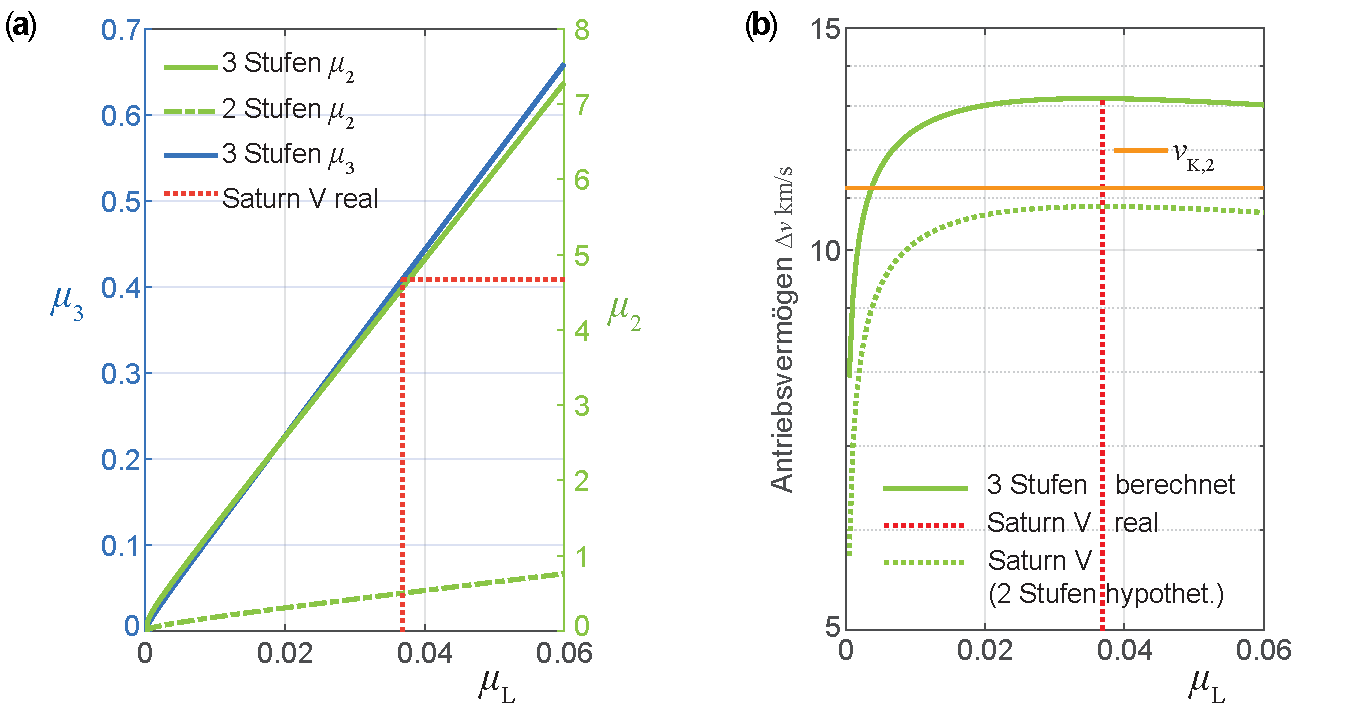
\includegraphics[width=\textwidth]{RaketenOptimierung01.pdf} 
	\caption[Optimierung einer Dreistufen-Rakete.]{Optimierung einer Dreistufen-Rakete. L�sung �ber Extremwertberechnung. \fa Berechnung der Massenverh�ltnisse der einzelnen Raketenstufen \fb Antriebsverm�gen f�r eine Dreistufen-Rakete (berechnet) und f�r die Saturn V. Zum Vergleich sind auch die Werte f�r eine (hypothetische) Ausf�hrung der Saturn V als Zweistufen-Rakete gezeigt.}
	\label{abb:adyn_optrockets01}
\end{figure}

\item \textit{\textbf{L�sungsansatz �ber Lagrange-Multiplikatoren - Beispiel Saturn V zum Mond}}\\ 
	
	Gegeben seien nach Aufgabenstellung: $v_{\text{G},i}$ (Ausstr�mgeschwindigkeit), $\sigma_i$ (Strukturparameter) und $m_0$ (Gesamtmasse der Rakete) \\
Variiert werden k�nnen die Massenverh�ltnisse $\mu_i$ oder, was gleichbedeutend ist, die Teil-Nutzlastverh�ltnisse $\eta_i$, die wir �ber
\begin{align}
    \eta_i = \frac{m_{\text{L},i}}{m_{0,i}-m_{0,i+1}} = \frac{m_{0,i+1}}{m_{\text{S},i} + m_{\text{T},i}} \label{adyn_optrocket11}
\end{align}
definieren. \\
Als $i$-tes Nutzlastverh�ltnis wird die Masse der n�chsten $\lk i+1\rk$-ten Unterrakete im Verh�ltnis zur Summe von Struktur- und Treibstoffmasse der $i$-ten Stufe definiert. Die Zahl der Stufen k�nnte ebenfalls variiert werden, soll aber hier festgehalten werden. \\
Zu optimieren/maximieren sind das Gesamt-Nutzlastverh�ltnis $\mu_\text{L}$ und das Gesamt-Antriebsverm�gen $\Delta v$, also max $\mu_\text{L}\lk \Delta v\rk$ \bzw max $\Delta v\lk\mu_\text{L}\rk $.\\
In Kapitel �ber den Lagrange-Formalismus im Band I hatten wir die Methode der Lagrange-Multiplikatoren kennen gelernt, mit der man die Extremwertberechnung der Wirkung $S$ bei Vorliegen von Zwangsbedingungen \bzw Nebenbedingungen durchf�hren konnte. Wir wenden dies f�r unser Problem an. Der Wirkung $S$ entspricht hier die Gr��e $\mu_\text{L}$ \bzw $\Delta v$, die Nebenbedingungen sind duch die $m_{\text{S},i}$ \bzw $\sigma_{i}$ gegeben und die "`Bewegungsgleichungen"' ergeben sich dann durch:
\begin{align}
    \frac{\d\lk\mu_\text{L}\rk}{\d \eta_j} + \lambda_{\mu_\text{L}}\,\frac{\d\lk \Delta v\rk}{\d \eta_j} = 0 ~~~~ \text{(maximieren von $\mu_\text{L}$)} \label{adyn_optrocket12}
\end{align}
\bzw
\begin{align}
    \frac{\d\lk\Delta v\rk}{\d \eta_j} + \lambda_{\Delta v}\,\frac{\d\lk \mu_\text{L}\rk}{\d \eta_j} = 0 ~~~~ \text{(maximieren von $\Delta v$)} \,.\label{adyn_optrocket13}
\end{align}
F�r $\lambda_{\mu_\text{L}} = 1/\lambda_{\Delta v}$ beschreiben beide Gleichungen das gleiche mathematische Problem.\\
Wir f�hren die Ableitungen aus und erhalten:
\begin{align}
\begin{split}
     \frac{\d\lk\Delta v\rk}{\d \eta_j} &= -v_{\text{G,j}}\,\frac{1-\sigma_j}{1+\eta_j}\,\frac{1}{\sigma_j+\eta_j} \,,\\
     \frac{\d\lk\mu_\text{L}\rk}{\d \eta_j}  &= \frac{\mu_\text{L}}{\eta_j\lk 1+\eta_j\rk}
\end{split}\label{adyn_optrocket14}
\end{align}
und erhalten aus \eqref{adyn_optrocket12}
\begin{align}
    \frac{\mu_\text{L}}{\eta_j\lk 1+\eta_j\rk} = \lambda_{\mu_\text{L}}\,v_{\text{G},j}\,\frac{1-\sigma_j}{1+\eta_j}\,\frac{1}{\sigma_j + \eta_j} \label{adyn_optrocket15} \,.
\end{align}
Daraus folgt sofort
\begin{align}
    v_{\text{G},j}\,\eta_j\,\frac{1-\sigma_j}{\sigma_j + \eta_j} = \frac{\mu_\text{L}}{\lambda_{\mu_\text{L}}} =:\gamma = \text{const} ~~~~ j=1,2,\ldots,N \,.\label{adyn_optrocket16}
\end{align}
Damit haben wir die Grundgleichungen f�r die Optimierung. \\
$\gamma$ ist noch eine unbekannte Gr��e, die es aus \eqref{adyn_optrocket16} zu bestimmen gilt. Wir nehmen diese zun�chst als bestimmt an, so dass sich dann die optimalen Nutzlastverh�ltnisse ergeben zu:
\begin{align}
    \eta_\text{j,\text{opt}} = \frac{\gamma\,\sigma_j}{\lk 1-\sigma_j\rk\,v_{\text{G},j}-\gamma}~~~~ j=1,2,\ldots,N \,.\label{adyn_optrocket17}
\end{align}
Wir setzen diese in die Raketen-Gleichung f�r die serielle Stufung \eqref{eq:adyn_rockets17} ein und erhalten:
\begin{align}
    \Delta v = \sum\limits_{j=1}^N\,v_{\text{G},j}\,\ln\,\frac{1+\eta_j}{\sigma_j + \eta_j} = \sum\limits_{j=1}^Nv_{\text{G},j}\,\ln\,\frac{v_{\text{G},j}-\gamma}{\sigma_j\,v_{\text{G},j}}\,.\label{adyn_optrocket18}
\end{align}
F�r das totale Nutzlastverh�ltnis 
\begin{align}
    \mu_\text{L} = \frac{m_\text{L}}{m_0} = \prod\limits_{j=1}^N\frac{\eta_j}{1+\eta_j} = \prod\limits_{j=1}^N \frac{\gamma\,\sigma_j}{\lk 1-\sigma_j\rk\lk v_{\text{G},j}-\gamma\rk}\,.\label{adyn_optrocket19}
\end{align}
Der weitere Weg besteht darin, dass man aus \eqref{adyn_optrocket18} f�r bekannte $\sigma_j$, $\Delta v$ die Konstante $\gamma$ (die aus dem Lagrange-Multiplikator abgeleitet wurde) bestimmt und diese in \eqref{adyn_optrocket19} einsetzt, um $\mu_\text{L,opt}$ zu erhalten. \\
Die Konstante $\gamma$ muss aus der Gleichung \eqref{adyn_optrocket16} numerisch bestimmt werden, was wir vorteilhaft in \matlab\,im Skript \mladynref{RaketenOptimierung02.m} ausgef�hrt haben.\\
Wenn wir die in der �bung in Tabelle \ref{tab:adyn_parameter_Apollo11} angegebenen Werte verwenden, erhalten wir aus der Rechnung einen Wert von $\mu_\text{L} = 0.0176$, der nur wenig von dem tats�chlichen (etwas kleineren) Wert von $\mu_\text{L} = 0.0162$ abweicht, mit dem die NASA (vermutlich aus Sicherheitsgr�nden) operierte.
In \figref{adyn_optrockets02} ist das maximale Nutzlastverh�ltnis gezeigt, mit der eine Nutzlast von $m_\text{L} = \mu_\text{L,opt}\cdot m_0$ auf ein bestimmtes Antriebsverm�gen gebracht werden kann.\\
Es sei noch darauf hingewiesen, dass $\gamma < \mathrm{min}\lk v_{\text{G},j}\,\lk 1-\sigma_j\rk \rk \,$f�r alle $j=1,\ldots,N$ sein muss, was bei der numerischen Berechnung zu ber�cksichtigen ist.
	
\begin{figure}[H]
	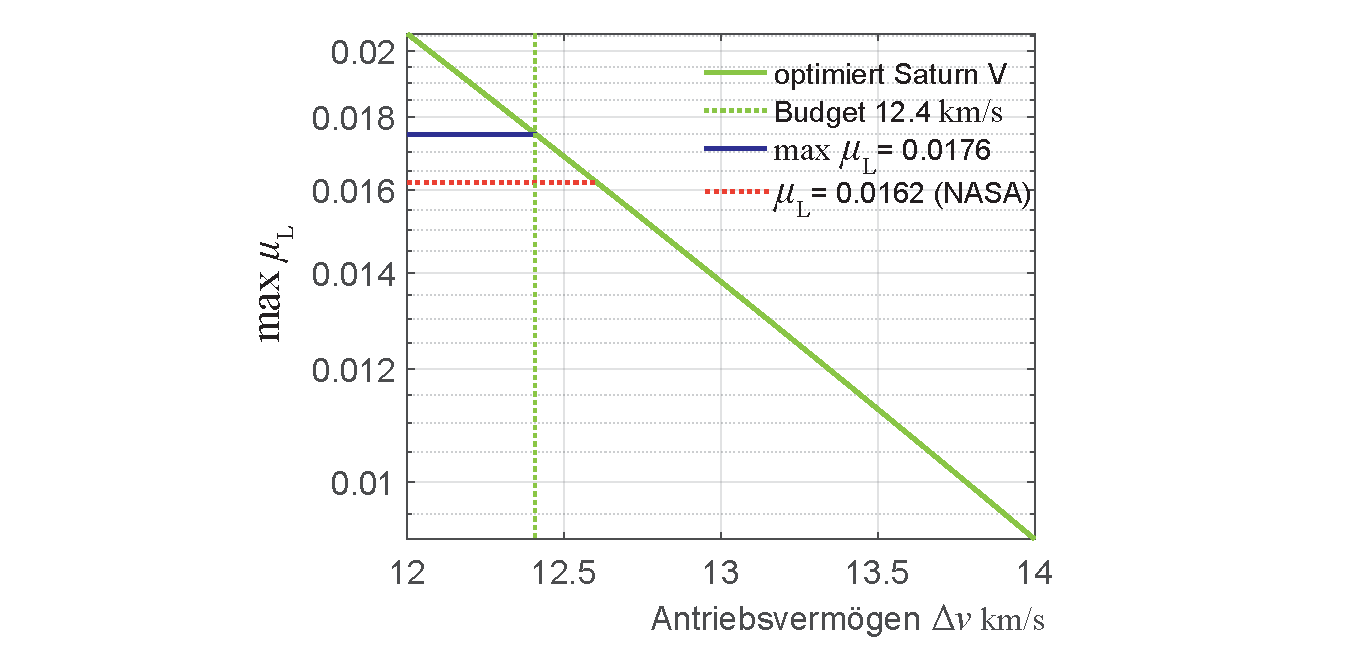
\includegraphics[width=\textwidth]{RaketenOptimierung02.pdf} 
	\caption[Optimierung einer Dreistufen-Rakete.]{Optimierung Saturn V Konfiguration f�r die Apollo Missionen. L�sung �ber Methode der Lagrange-Multiplikatoren. Berechnung des optimalen Antriebsverm�gens/Nutzlastverh�ltnisses.}
	\label{abb:adyn_optrockets02}
\end{figure}


\end{enumerate}

\end{sol} 
\textcolor{blue} {$\rightarrow$ zur} \probref{adyn_rocketopt1}.\\
\noindent\rule[1ex]{\textwidth}{0.5pt}  \newpage  \clearpage


%-----------------------------------------------------------------------------------------------------------


\begin{sol}{prob:adyn_rocketopt2}\label{lsg:adyn_rocketopt2} %�bung4
\textbf{Vergleich Mehrstufenrakete (Serielle und Parallelstufung)} \\ \\
Wir fassen die Vor- und Nachteile der Tandemstufung gegen�ber der Parallelstufung  in der folgenden Tabelle zusammen.\\
\begin{table}%tab1
\caption{Vor- und Nachteile der Tandemstufung gegen�ber der Parallelstufung.}
\smallskip
\hspace{1.5cm}
\begin{tabular}{L{3cm}L{3cm}L{3cm}}
\svhline\noalign{\smallskip}
Eigenschaft				    			& Tandemstufung				& Parallelstufung \\
\noalign{\smallskip}\svhline\noalign{\smallskip}
\noalign{\smallskip}
Startbeschleunigung							&kleiner &gr��er\\	
Strukturbelastung 							&kleiner &gr��er\\	
Biegemomente      							&gr��er  &kleiner\\	
Aerodynamische Verluste 				&kleiner &gr��er\\	
Gravitationsverluste						&gr��er  &kleiner\\	
Gesamtl�nge Rakete							&gr��er  &kleiner\\	
\noalign{\smallskip}
\svhline\noalign{\smallskip}
\end{tabular} \\
\label{tab:adyn_vergleich_staging}
\end{table}%tab1


\end{sol} 
\textcolor{blue} {$\rightarrow$ zur} \probref{adyn_rocketopt2}.\\
\noindent\rule[1ex]{\textwidth}{0.5pt}  \newpage  \clearpage


%-----------------------------------------------------------------------------------------------------------


%-----------------------------------------------------------------------------------------------------------
%-----------------------------------------------------------------------------------------------------------

\subsection{�bungen zu Umlaufbahnen}

\medskip

%-----------------------------------------------------------------------------------------------------------

\begin{sol}{prob:adyn_orbits1}\label{lsg:adyn_orbits1} %�bung5
\textbf{Bahnparameter aus Bodenbeobachtungen}\\ \\
\textit{Bahnparameter von Satelliten mit gegebenen geozentrischen Orts- und Geschwindigkeitsdaten:}\\ \\
Wir verwenden die Formeln aus \kap{adyn_orbits_determination_rv} und erhalten:\\

Satellit 1 (HEO)
\begin{align*}
	&\text{Halbachse}\,\,a & \SI{20251.57}{\km}\\
	&\text{Exzentrizit�t}\,\,e & 0.777596\\
	&\text{Bahnneigung} \,\,i &   10.194 \degree\\
	&\text{Knoten} \,\, \Omega &  171.951 \degree\\
	&\text{Arg. Perig�um} \,\, \omega &  86.081 \degree\\
	&\text{Mittl. Anomalie} \,\, M &  138.824  \degree\\
	&\text{Mittl. Bewegung} \,\, n & \SI{2.19e-04}{\per\second} \\
\end{align*}

Satellit 2 (LEO)
\begin{align*}
	&\text{Halbachse}\,\,a & \SI{8225.40}{\km}\\
	&\text{Exzentrizit�t}\,\,e & 0.076722\\
	&\text{Bahnneigung} \,\,i &   6.707 \degree\\
	&\text{Knoten} \,\, \Omega &  145.881 \degree\\
	&\text{Arg. Perig�um} \,\, \omega &  86.476 \degree\\
	&\text{Mittl. Anomalie} \,\, M &  167.278  \degree\\
	&\text{Mittl. Bewegung} \,\, n & \SI{8.46e-04}{\per\second}
\end{align*}

\newpage

\textit{Bahnparameter der ISS aus den ver�ffentlichten geozentrischen Orts- und Geschwindigkeitsdaten der NASA:}\\
	%\url{https://spotthestation.nasa.gov/trajectory_data.cfm}\\

Auch hier verwenden wir die Formeln aus \kap{adyn_orbits_determination_rv} und erhalten:
\begin{align*}
	&\text{Halbachse}\,\,a & \SI{6803.28}{\km}\\
	&\text{Bahnh�he}\,\,h & \SI{425.28}{\km}\\
	&\text{Exzentrizit�t}\,\,e & 0.001855\\
	&\text{Bahnneigung} \,\,i &  51.751 \degree\\
	&\text{Knoten} \,\, \Omega &  47.685 \degree\\
	&\text{Arg. Perig�um} \,\, \omega & 124.00 \degree\\
	&\text{Mittl. Anomalie} \,\, M & 315.75 \degree\\
	&\text{Umlaufzeit} \,\, n & \SI{93.8 }{\minute}
\end{align*}
Die mittlere Anomalie $M$ wurde so angepasst, dass der Anfangswert mit den NASA Daten �bereinstimmt. Wir verweisen auf \kap{adyn_orbits_determination_singulaer}
zur Berechnung alternativer Bahnparameter bei kreisf�rmigen und �quatorialen Bahnen, sowie auf die Zusatzaufgabe \probref{adyn_orbits_zusatz1}.
\begin{figure}[H]
	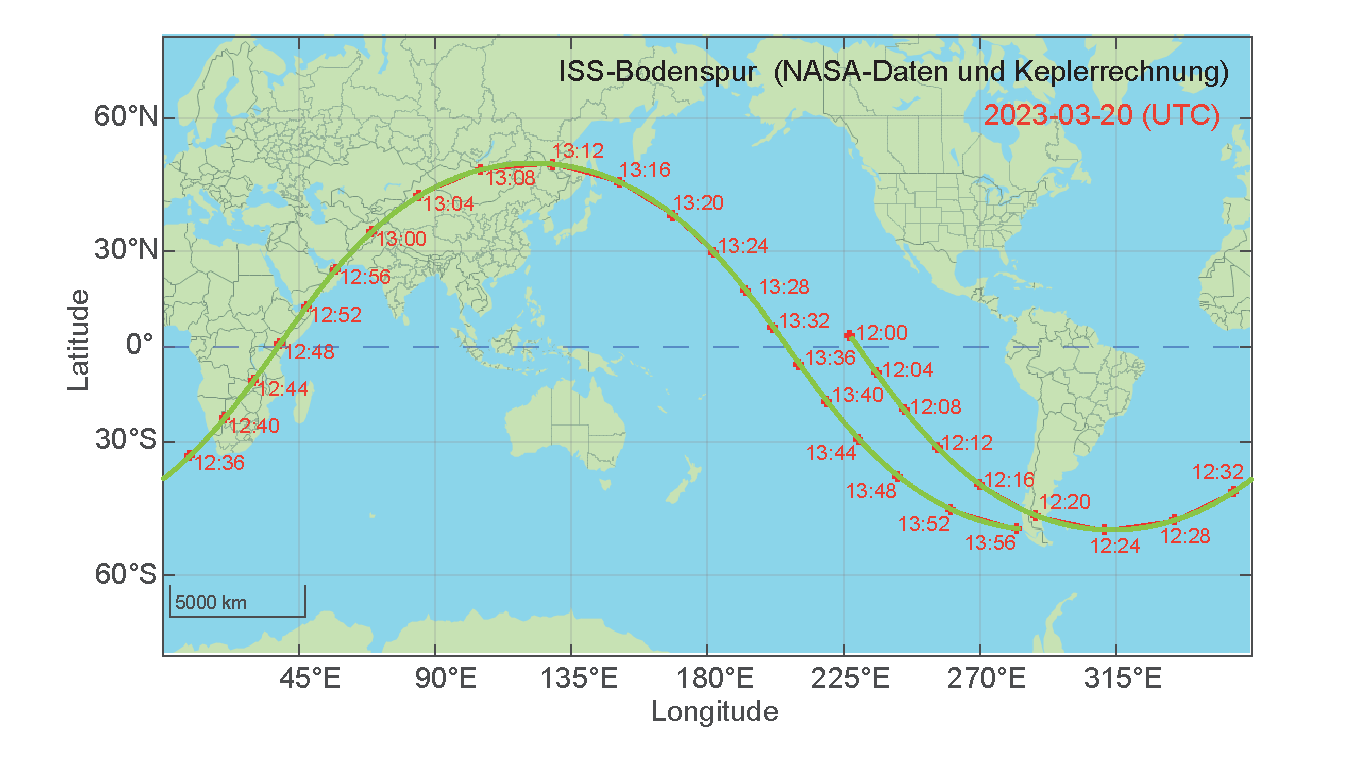
\includegraphics[width=\textwidth]{GroundTrackISS20032023.pdf} 
	\caption[Bodenspur der ISS.]{Bodenspur der ISS. Vergleich NASA Daten und Berechnung Keplerbahn.}
	\label{abb:adyn_satobserv02}
\end{figure}
Die Berechnungen finden sich im Detail im \mscr{} \mladynref{BahnparaBestimmung01.m}. 

\end{sol} 
\textcolor{blue} {$\rightarrow$ zur} \probref{adyn_orbits1}.\\
\noindent\rule[1ex]{\textwidth}{0.5pt}  \newpage  \clearpage

%-----------------------------------------------------------------------------------------------------------
\newpage

\begin{sol}{prob:adyn_orbits2}\label{lsg:adyn_orbits2} %�bung6
\textbf{Bodenspuren von Erdsatelliten}\\ 

\begin{itemize}
	\item \textit{\textbf{Bodenspuren verschiedener Satellitenarten}}\\
		\begin{itemize}
			\item Bodenspur eines GEO-Satelliten.
			\item Bodenspur eines Molnija-Satelliten (HEO-Satelliten).
			\item Bodenspur eines polaren Satelliten. 
		\end{itemize}
		\begin{figure}[H]
			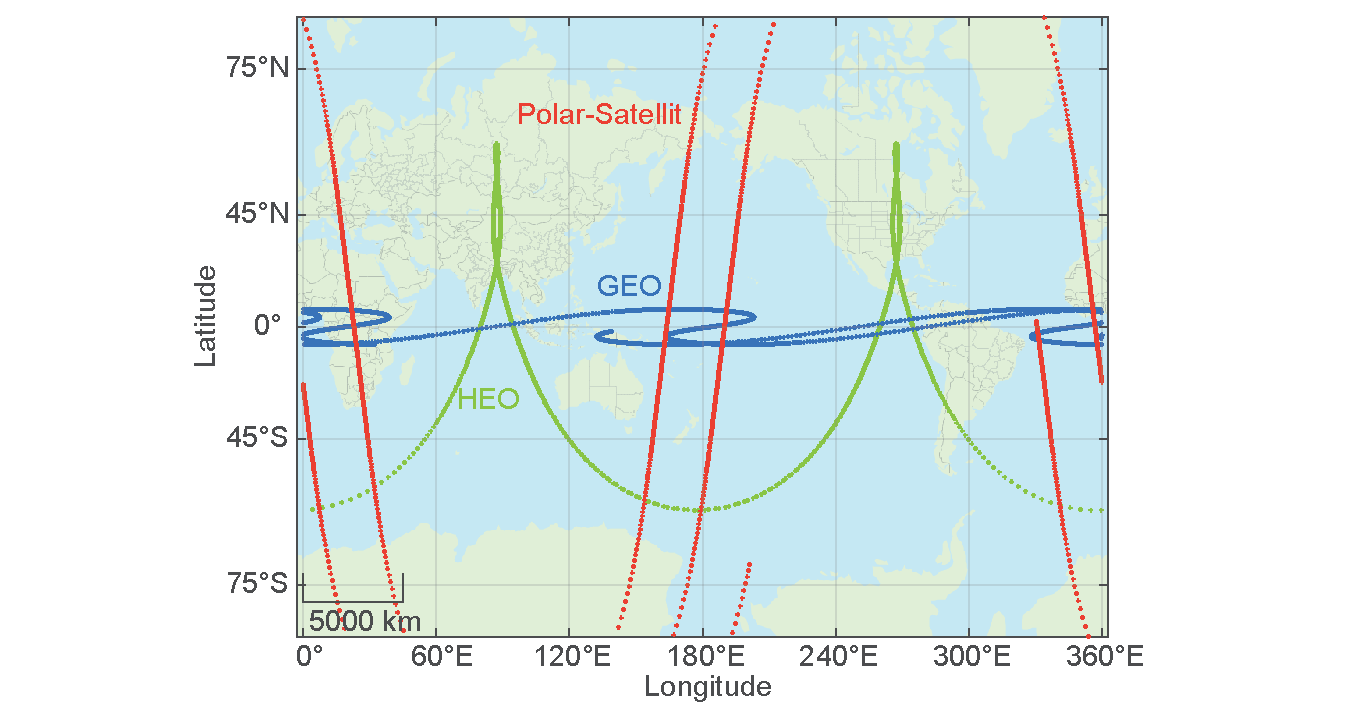
\includegraphics[width=0.9\textwidth]{Orbits03a.pdf} 
			\caption[Bodenspuren von verschiedenen Satelliten.]{Bodenspuren von verschiedenen Satelliten. GEO:\, $a = \SI{25000}{\km},\, e = 0.73,\, i = 8\degree,\, \Omega =45\degree$,\,\, HEO (Typ Molnija-Satelliten):\, $a = \SI{26555}{\km},\, e = 0.72,\, i = 63.4\degree,\, \Omega =120\degree,\,\omega =270\degree$,\,\, Polar-Satellit:\, $a = \SI{7330}{\km},\, e = 0.0,\, i = 93\degree,\, \Omega =130\degree,\,\omega =0\degree$.}
			\label{abb:adyn_orbits03a}
			\end{figure}
	\item \textit{\textbf{Bodenspuren verschiedener Satelliten in geosynchronen Umlaufbahnen}}\\

				Die Bodenspuren \figref{adyn_orbits03b} �hneln den verschiedenen Analemma, die wir im \kap{kulmination_sonne} \bzw in der \probref{hm_Analemma_Mars} kennen gelernt hatten. Das ist nicht verwunderlich. In einer geozentrischen Betrachtung �bernehmen die Satelliten die Rolle der Sonne, die unterschiedlichen Formen des \textit{\anf{Satelliten-Analemmas}} kommen durch die unterschiedlichen Bahnparameter zustande. Siehe auch im Detail \probref{hm_Analemma_Mars}.\\
\newpage
			\begin{figure}[H]
			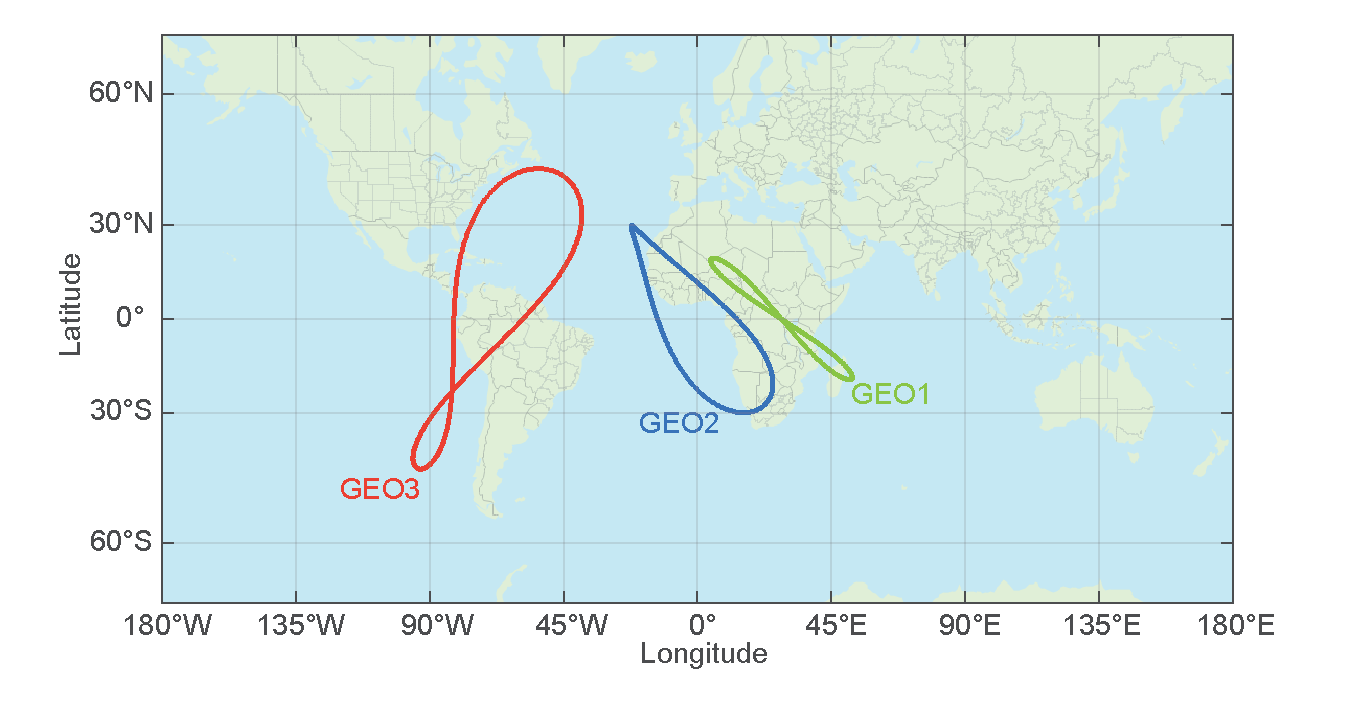
\includegraphics[width=0.95\textwidth]{Orbits03b.pdf} 
			\caption[Bodenspuren von verschiedenen geosynchronen Satelliten.]{Bodenspuren von verschiedenen geosynchronen Satelliten. Parameter siehe \probref{adyn_orbits2}.}
			\label{abb:adyn_orbits03b}
			\end{figure}
\item \textit{\textbf{Bodenspur ISS}}\\
			\begin{figure}[H]
			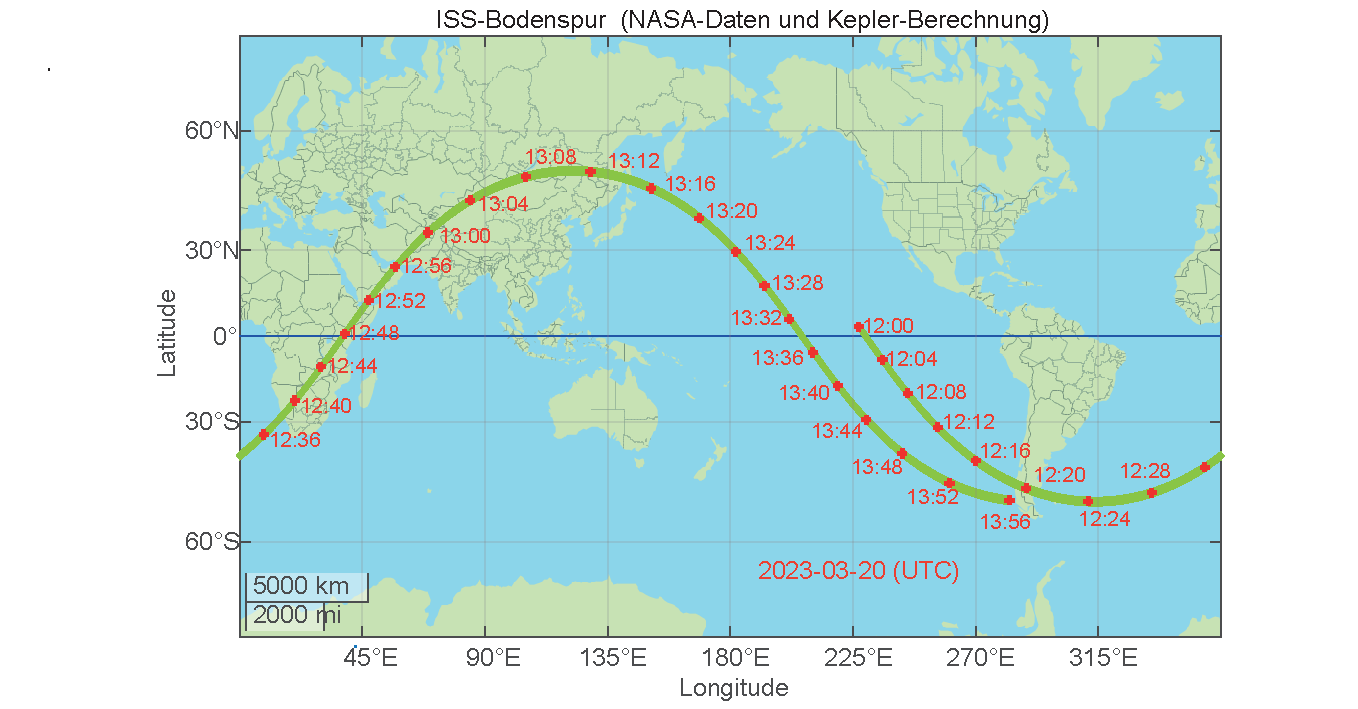
\includegraphics[width=0.95\textwidth]{ISSBodenspur.pdf} 
			\caption[Bodenspuren der ISS.]{Bodenspuren der ISS vom 20.03.2023. Parameter siehe \probref{adyn_orbits2}.}
			\label{abb:adyn_orbits03c}
			\end{figure}
\end{itemize}
Die Berechnungen finden sich im Detail im \mscr~\mladynref{SatPositionen01.m} \bzw \mladynref{SatPositionen02.m}.

\end{sol} 
\textcolor{blue} {$\rightarrow$ zur} \probref{adyn_orbits2}.\\
\noindent\rule[1ex]{\textwidth}{0.5pt}  \newpage  \clearpage

%-----------------------------------------------------------------------------------------------------------

\begin{sol}{prob:adyn_orbits3}\label{lsg:adyn_orbits3} %�bung7
\textbf{Bodenbeobachtung von Erdsatelliten}\\ \\

Die Berechnungen finden sich im Detail im \mscr~\mladynref{SatPositionen03.m} \bzw \mladynref{SatPositionen04.m}.
\begin{figure}[H]
	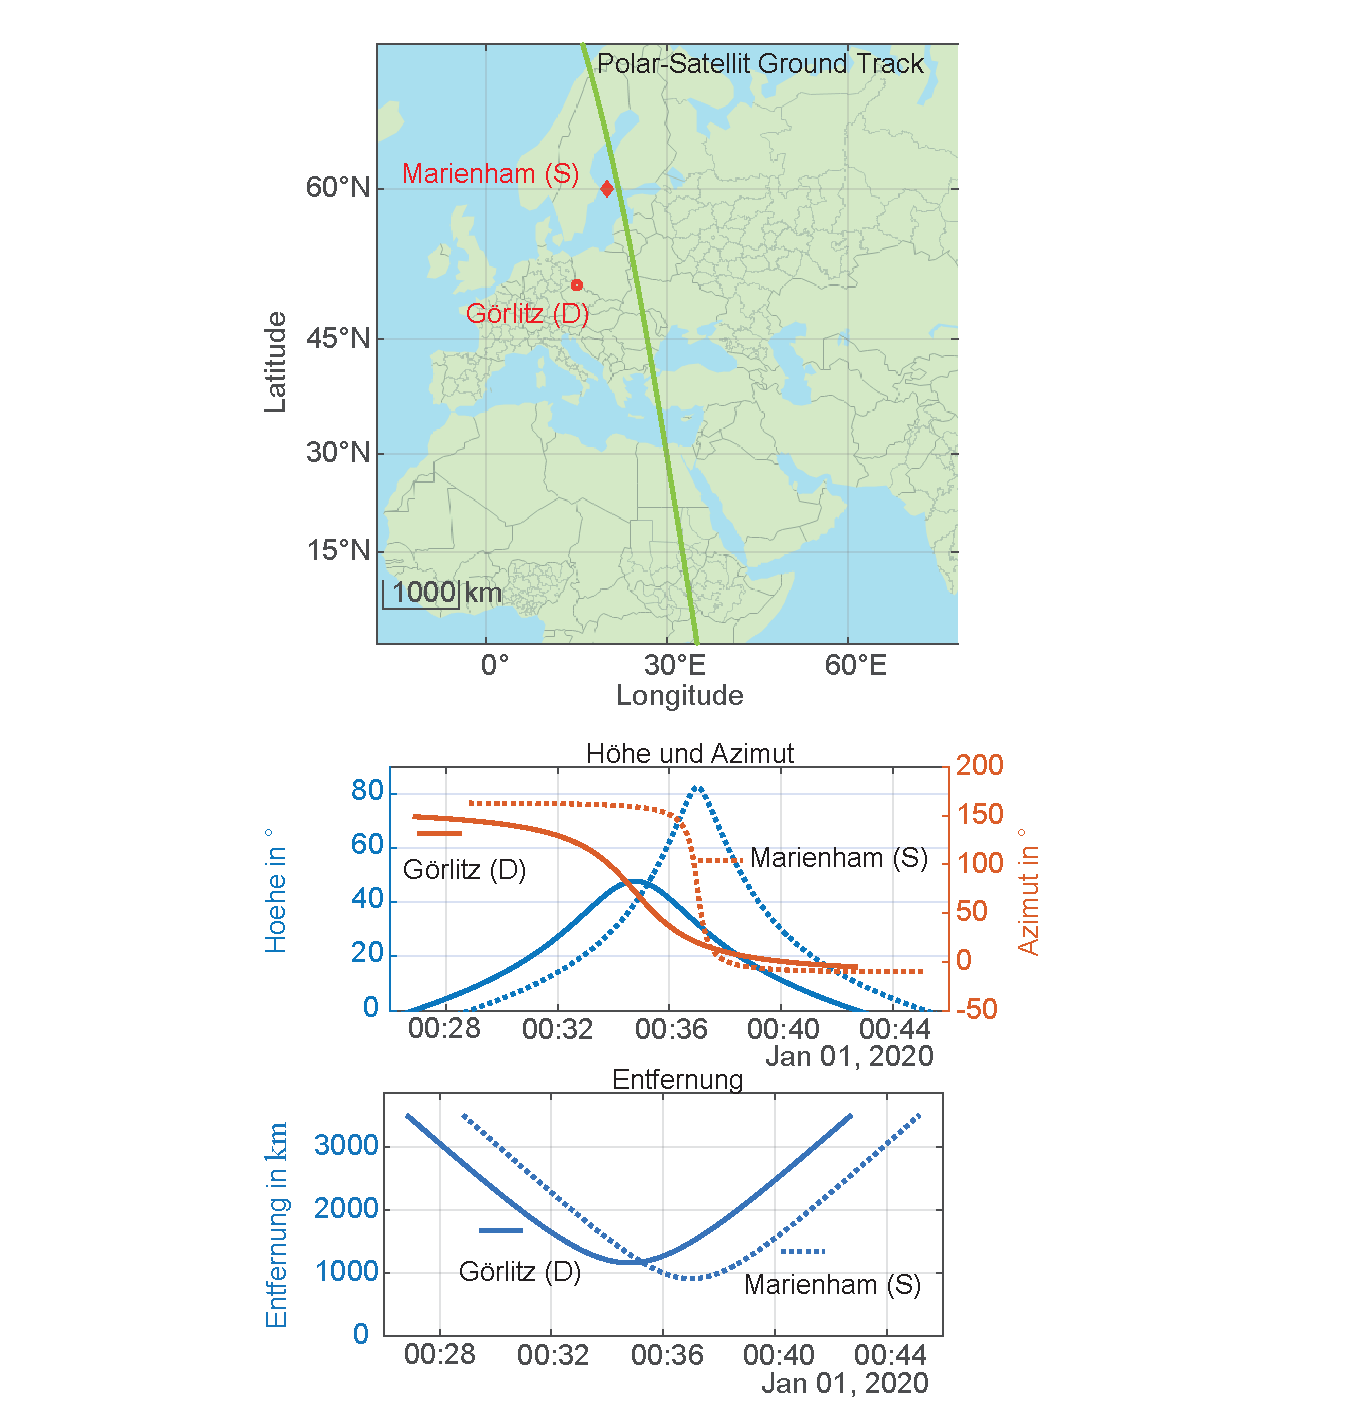
\includegraphics[width=\textwidth]{TopographPolarerSat.pdf} 
	\caption[Topographische Beobachtung eines polaren Satelliten.]{Bodenspur, Azimut, H�he und Entfernung eines polaren Satelliten von zwei Bodenstationen. Parameter siehe \probref{adyn_orbits3} und \mscr~\mladynref{SatPositionen03.m} \bzw \mscr~\mladynref{SatPositionen03a.m}.}
	\label{abb:adyn_satobserv03}
\end{figure}
\begin{figure}[H]
	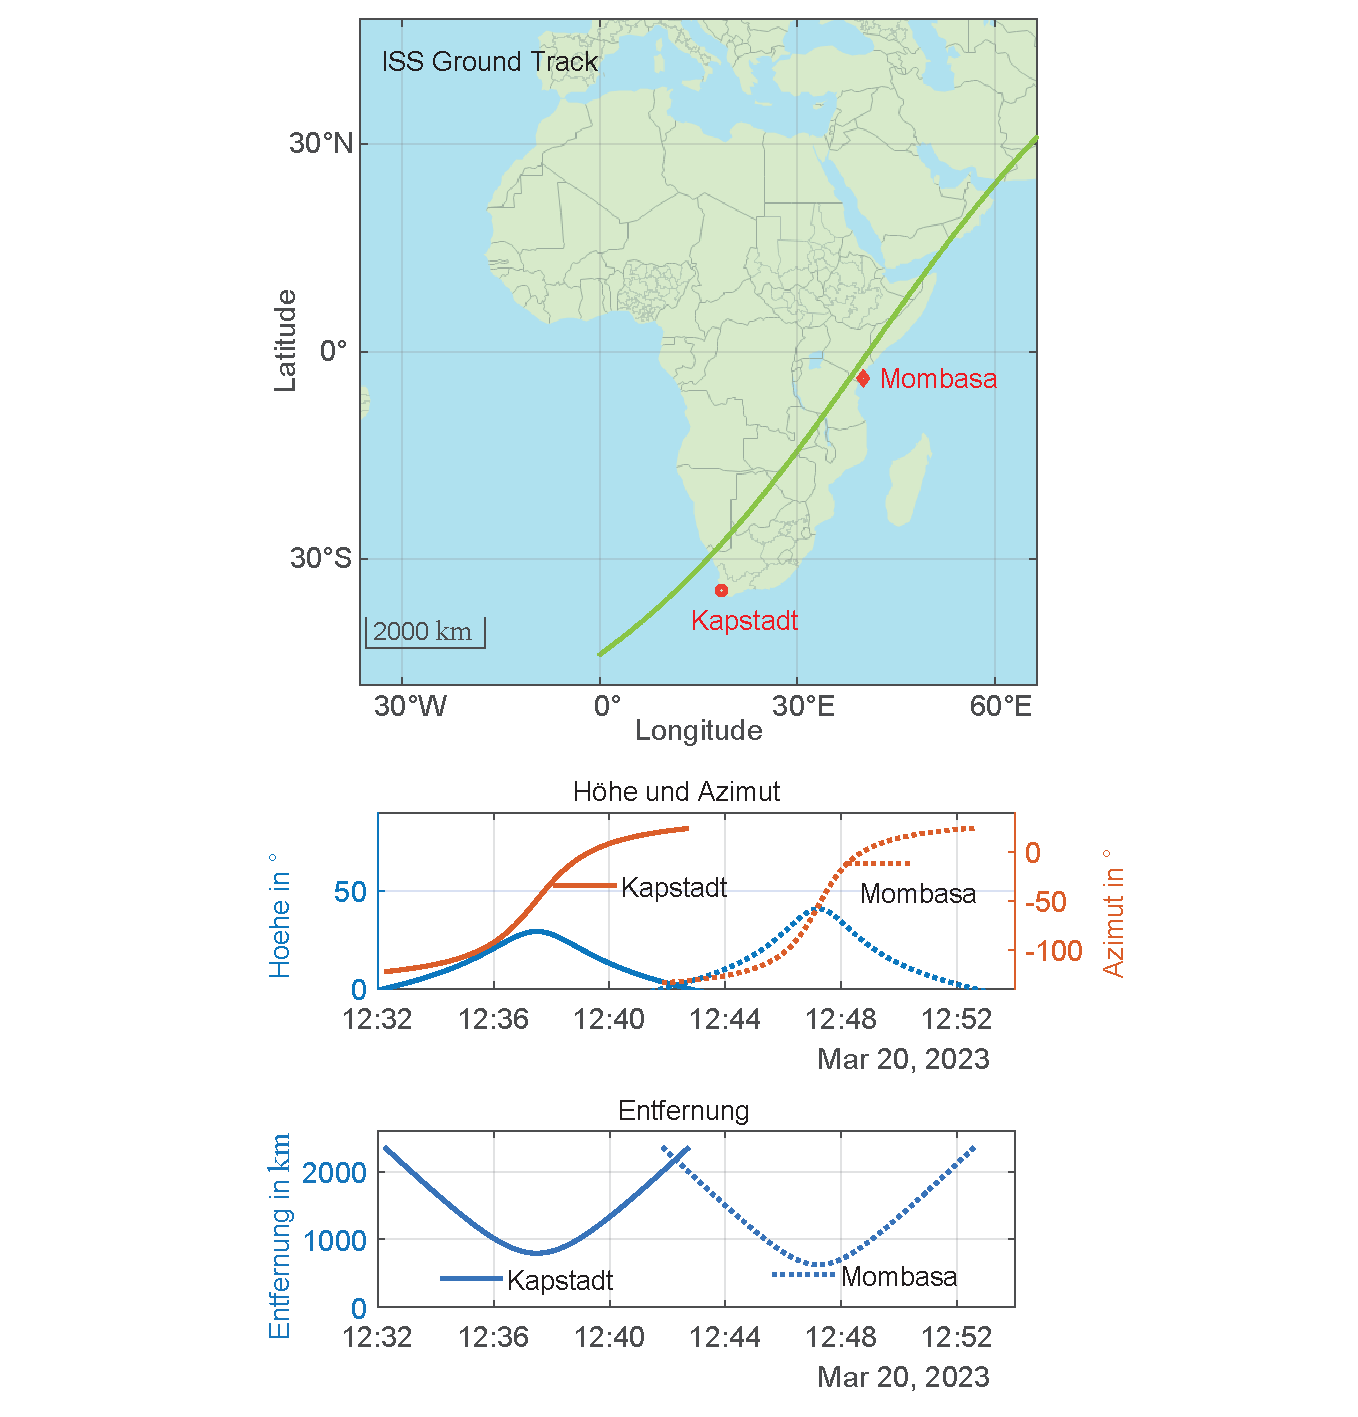
\includegraphics[width=\textwidth]{TopographISS.pdf} 
	\caption[Topographische Beobachtung der ISS.]{Bodenspur, Azimut, H�he und Entfernung der von zwei Bodenstationen. Parameter siehe \probref{adyn_orbits3} und \mscr~\mladynref{SatPositionen04.m}.}
	\label{abb:adyn_satobserv04}
\end{figure}

\end{sol} 
\textcolor{blue} {$\rightarrow$ zur} \probref{adyn_orbits3}.\\
\noindent\rule[1ex]{\textwidth}{0.5pt}  \newpage  \clearpage

%-----------------------------------------------------------------------------------------------------------

\begin{sol}{prob:adyn_orbits4}\label{lsg:adyn_orbits4} %�bung8
\textbf{Bodenbeobachtung eines Molniya-Satelliten}\\ \\

Die Berechnungen finden sich im Detail im \mscr~\mladynref{SatPositionen05.m}.
\begin{figure}[H]
	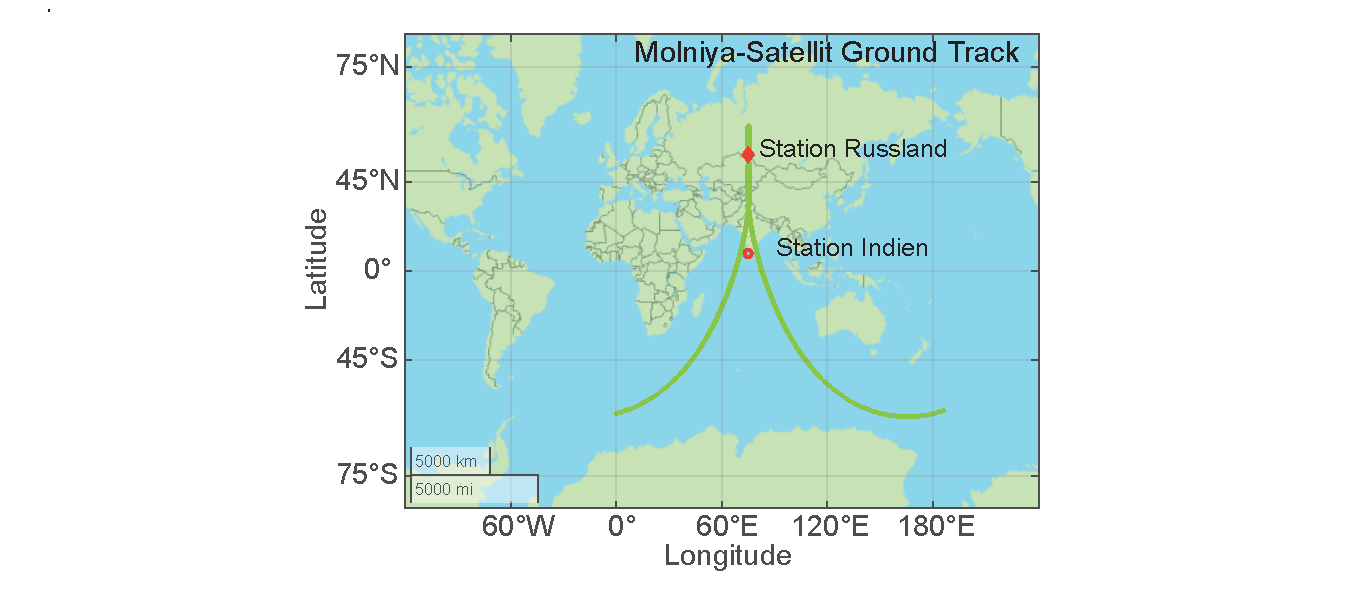
\includegraphics[width=\textwidth]{TopographMolniyaSat01.pdf} 
	\caption[Bodenspur eines Molniya-Satelliten.]{Bodenspur eines Molniya-Satelliten.\\Parameter siehe \probref{adyn_orbits4} und \mscr~\mladynref{SatPositionen05.m}.}
	\label{abb:adyn_MolniyaObserv01}
\end{figure}
\begin{figure}[H]
	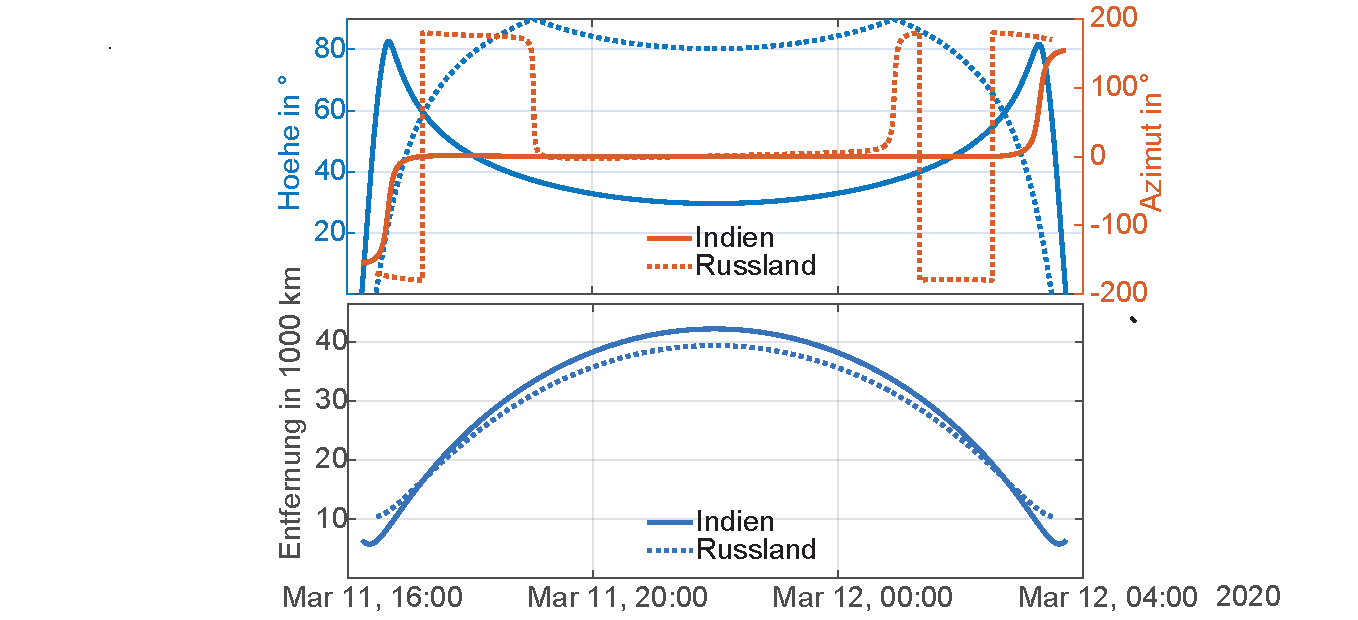
\includegraphics[width=\textwidth]{TopographMolniyaSat02.pdf} 
	\caption[Topographische Beobachtung eines Molniya-Satelliten.]{Azimut, H�he und Entfernung eines Molniya-Satelliten von zwei Bodenstationen. Parameter siehe \probref{adyn_orbits4} und \mscr~\mladynref{SatPositionen05.m}.}
	\label{abb:adyn_MolniyaObserv02}
\end{figure}
\end{sol} 
\textcolor{blue} {$\rightarrow$ zur} \probref{adyn_orbits4}.\\
\noindent\rule[1ex]{\textwidth}{0.5pt}  \newpage  \clearpage


%-----------------------------------------------------------------------------------------------------------

\begin{sol}{prob:adyn_orbits5}\label{lsg:adyn_orbits5} %�bung9
\textbf{Sonnensynchrone Bahnen}\\ \\

Die Drehimpulserhaltung gilt streng nur f�r das Zweik�rperproblem, dann ist auch die Bahnebene fest im Raum orientiert und die Bahn geschlossen.\\
Wie wir \zb in \kap{Periheldrehung} gesehen haben, bewirkt die Abplattung der Erde jedoch ein Drehmoment auf die Bahn und f�hrt zu einer Verschiebung der Rektaszension des aufsteigenden Knotens. 
Man kann mit Hilfe der St�rungsrechnung zeigen (siehe auch \probref{adyn_pertubations}), dass die Frequenz dieser Pr�zession des aufsteigenden Knoten sich nach folgender Formel berechnet:
	\begin{align}
		\dot{\Omega} = -\frac{3}{2} J_2\, \frac{2\pi}{T_\text{E}} \lk \frac{R_\text{E}}{a\,(1-e^2)} \rk^2 \cos i = 
		-\frac{3}{2} J_2\,R_\text{E}\, \sqrt{\frac{a_\text{E}}{a_\text{E}{}^2}} \, \frac{\cos i}{a^2\,(1-e^2)^2} = C\,f(a,e,i)\,. \label{eq:adyn_orbits5_01}
	\end{align}
Hierin sind $J_2$ die sogenannte zonale Harmonische\index{Harmonische!zonale} (siehe \kap{adyn_gravity_pertubations}) als Ma� f�r die Abplattung der Erde, $R_\text{E}$ der mittlere Erdradius, $a$ die gro�e Halbachse der Satellitenbahn und $i$ \bzw $e$ deren Neigung (Inklination) \bzw Exzentrizit�t. $T_\text{E} = 2\pi\sqrt{a_\text{E}{}^3/\mu_\text{E}}$ ist die Umlaufzeit der Erde um die Sonne.\footnote{Genauer gesagt ist es die Zeit eines anomalistischen Jahres ($\SI{365.25963}{}\,\mathrm{d}$, siehe \kap{hm_zeitdefinition})} Die Pr�zession ist umso gr��er, je geringer die Inklination $i$ und die Bahnh�he $a$ sind.\\
Wegen des Minuszeichen wirkt bei einer retrograden Bahnen (Bahn entgegen der Erdrotation, \dh $i > 90\degree$) diese Pr�zession in die gleiche Richtung wie die Erdrotation. Man kann also durch geeigneter Wahl von Inklination und Flugh�hen daf�r sorgen, dass sich die Bahn gerade um so viel verschiebt wie der mittleren Bewegung der Erde ($2\pi/T_\text{E}$) um die Sonne entspricht (\figref{adyn_synchron_orbit}). 

Bei einem SSO erfolgt der �berflug des Satelliten �ber einen Punkt auf der Oberfl�che des Planeten immer zur selben Ortszeit, vorausgesetzt die geographische Breite des Ortes liegt innerhalb des Bereiches, der durch die Inklination der Bahn begrenzt wird. Aufgrund dieser konstanten �berflugszeit lassen sich Beobachtungen von verschiedenen Tagen und Jahreszeiten gut miteinander vergleichen, deswegen haben ja Wetter- und Erdbeobachtungssatelliten oft solche Bahnen.

\begin{figure}[H]
	\includegraphics[width=\textwidth]{SonnensynchroneBahn.pdf} 
	\caption[Sonnensynchrone Bahn.]{Sonnensynchrone Bahn. Symbolische und nicht-ma�stabsgetreue Darstellung. }
	\label{abb:adyn_synchron_orbit}
\end{figure}

\newpage
\textbf{Zusatzaufgabe}\\

Wir wollen nun noch die Bodenspur des ERS-1 SSO-Satelliten berechnen \cite{Gottschalk1991}. Man k�nnte nun aus \eqref{eq:adyn_orbits5_01} einen der Parameter $a,\, e$ oder $i$ berechnen und die anderen vorgeben. 
Man hat aber eben mit $a$ einen weiteren Freiheitsgrad neben $i$, womit man auch fordern kann, dass die Bahnh�he $h$ so gew�hlt wird, dass ein �berflug �ber eine Gebiet (\zb das �berkreuzen des �quators nach $K$ Tagen \bzw. $N$ Orbits genau wiederholt (sogenannte \textit{Sonnensynchrone Repeat Orbits}).  Anfangs w�hlte man f�r den ERS-1 K=3, N=43, sp�ter ging man auf K=35.
Um das zu erreichen, muss man auch die St�rungen der Perihelverschiebung (siehe \kap{Stoerpotential_Merkur}) und der mittleren Anomalie ber�cksichtigen. Diese sind f�r kreisf�rmige Bahnen gegeben durch \cite{Montenbruck2012, Murray2008, Vallado2007}:

	\begin{align}
	\begin{split}
		\dot{\omega} = -\frac{3}{4} J_2\, n_0 \frac{R_\text{E}{}^2}{a^2} \lk 1 - 5\cos^2 i\rk \\ 
    \Delta n = n - n0  = -\frac{3}{4} J_2\, n_0 \frac{R_\text{E}{}^2}{a^2} \lk 1 - 2\cos^2 i\rk\,,
	\end{split}\label{eq:adyn_orbits5_02}
\end{align}

worin $n_0=\sqrt{(GM_\text{E}/a^3)}$ die mittlere Bewegung der Kepler-Bahn ist.
F�r sonnensynchrone Bahnen ist dann gefordert, dass gilt:

	\begin{align}
		\dot{\Omega} - \dot{\theta} = -360\degree\,, \\ 
\label{eq:adyn_orbits5_03}
\end{align}

woraus man f�r die Umlaufzeit einer solchen Bahn die Beziehung

	\begin{align}
		T_\text{P,SSO} = \frac{2\pi}{n_0-\Delta n-\dot{\omega}}\,, \\ 
\label{eq:adyn_orbits5_04}
\end{align}

was etwas l�nger ist als die Umlaufzeit im reinen Kepler-Fall.
Durch Iteration mit dem Startwert $T_\text{P,SSO}^{(0)}= 2\pi/n_0$ findet man �ber \eqref{eq:adyn_orbits5_02} aus \eqref{eq:adyn_orbits5_01} nacheinander $a$ und $i$ f�r die geforderten Bedingungen.\\

Wir finden:
\begin{align} 
  h &= a - R_\text{E} = \SI{7153.1}{\km} - \SI{6371.0}{\km} = \SI{782.1}{\km}\,, \\
	i &= 98.5\degree,
\end{align}
was f�r unsere Kreisbahnn�herung gut mit den Werten in \cite{Gottschalk1991} �bereinstimmt.
F�r die Berechnung der Bodenspur zu verschiedenen Zeiten, m�ssen Sie die Zeitabh�ngigkeit von $\Omega(t) = \Omega(t_0) + \dot{\Omega}\,(t-t_0)$ beachten.\\
Die Rechnungen finden sich im Detail im \mscr~\mladynref{SonnenSynchroneBahn.m} und ein Ergebnis in \figref{adyn_synchron_groundtrack}.

\begin{figure}[H]
	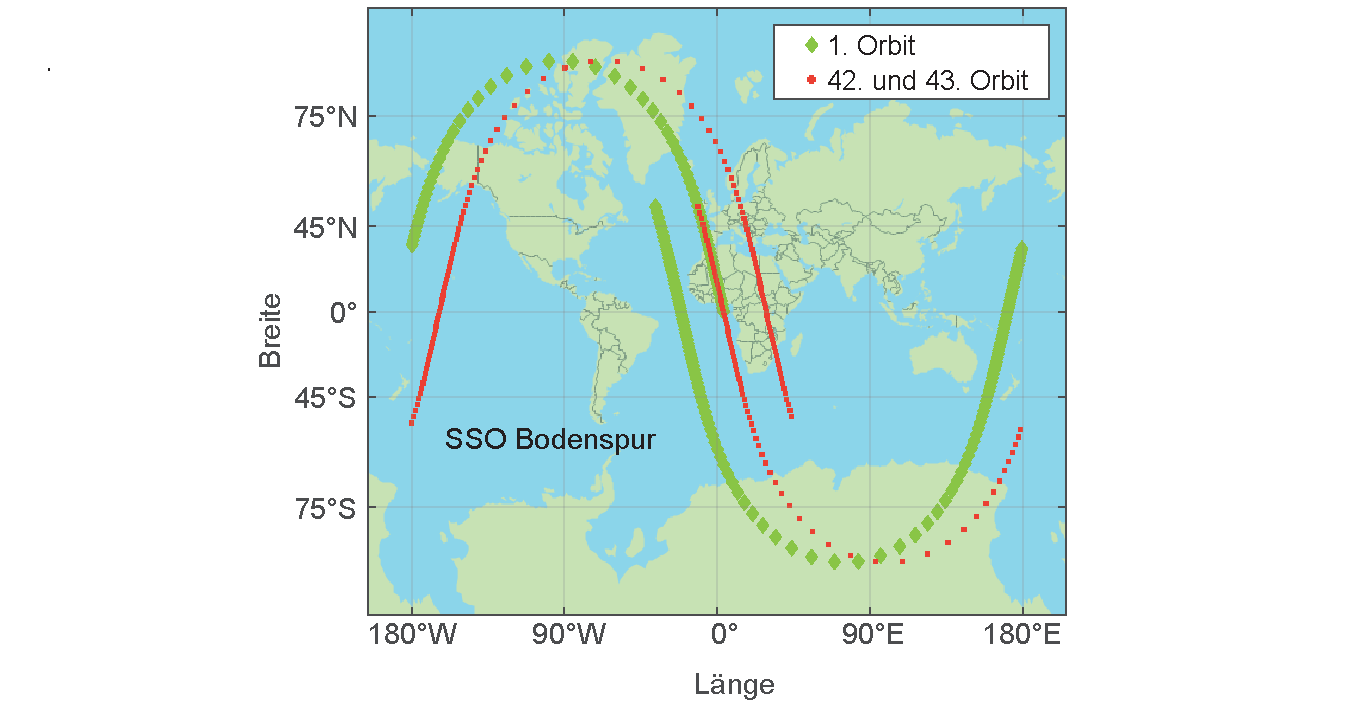
\includegraphics[width=\textwidth]{SonnensynchroneBodenspur.pdf} 
	\caption[Sonnensynchroner \textit{Repeat Orbit} -Bodenspur.]{Sonnensynchroner \textit{Repeat Orbit} - Bodenspur. Gezeigt sind Orbit Nr. 1 (willk�rlich gew�hlt) und die Orbits Nr 42 und Nr. 43 als Bodenspur. Man sieht, dass bei $N=43$ nach 3 Tagen der Satellit genau �ber die gleichen Gebiete fliegt wie beim Orbit $N=1$.}
	\label{abb:adyn_synchron_groundtrack}
\end{figure}

Wir empfehlen auch die Zusatz�bung \probref{adyn_pertubations}.

\end{sol} 
\textcolor{blue} {$\rightarrow$ zur} \probref{adyn_orbits5}.\\
\noindent\rule[1ex]{\textwidth}{0.5pt}  \newpage  \clearpage


%-----------------------------------------------------------------------------------------------------------

\begin{sol}{prob:adyn_starlink}\label{lsg:adyn_starlink} %�bung10
\textbf{Starlink}
\begin{figure}[H]
	\includegraphics[width=\textwidth]{StarlinkGeometrie.pdf} 
	\caption[Zur Geometrie der Starlink-Beobachtungen.]{[Zur Geometrie der Starlink-Beobachtungen. Mit rot ist die Kugelkappe dargestellt die ein Beobachter auf der Erde sieht, wenn sich ein Starlink-Satellit in einer Kugelschale mit Radius $R_\text{E} + h$ bewegt.}
	\label{abb:adyn_starlink_ueb01}
\end{figure}
\begin{enumerate}
\item [1)] Wir berechnen zun�chst den Anteil $\gamma\lk h\rk$ der Kugelschale mit Radius $R_\text{E} + h$, den ein Beobachter von der Erdoberfl�che aus sieht. \\
    Nach \figref{adyn_starlink_ueb01} ist das:
    \begin{align*}
        \gamma\lk h\rk = \frac{A_\text{KK}}{A_\text{K}} \,. 
    \end{align*}
    Hierin ist $A_\text{K}$ ist die Oberfl�che einer Kugel $4\pi\,r^2 = 4\pi\,\lk R_\text{E} +h\rk^2$ und $A_\text{KK}$ die Oberfl�che der Kugelkappe, die man sich leicht �ber 
    \begin{align*}
       A_\text{KK} &= 2\pi\,r\int\limits_{x_1}^{x_2} y(x)\,\sqrt{1+y'(x){}^2}\D x = 2\pi\int\limits_{\rho_1}^{\rho_2} y(\rho)\,\sqrt{1+y'(\rho){}^2}\,\D \rho 
    \end{align*}
    mit $y = \sqrt{r^2-x^2}$,\,  $1+y'{}^2 = r^2/(r^2-x^2)$,\, $r = R_\text{E} + h$\, und \,$x= \rho\,\cos\phi$ herleiten kann.\\
		Somit erh�lt man 
    \begin{align}
		  A_\text{KK} &= 2\pi\,r \int\limits_{R_\text{E}}^{R_\text{E} + h}\,\D \rho = 2\pi\,\lk R_\text{E} +h\rk \,h \nonumber \\
      \rightarrow~~~  \gamma\lk h\rk &= \frac{2\pi\,\killA{\lk R_\text{E} + h\rk}\,h}{4\pi\,\lk R_\text{E} + h\rk^\killA{2}} = \frac{1}{2}\,\frac{h}{R_\text{E} + h} \,. \label{eq:adyn_starlink_ueb01}
    \end{align}
    Mit den Angaben aus der Aufgabenstellung sind damit jederzeit pro Schale $n_i $ Satelliten 
    \begin{align*}
        n_i = \gamma\lk n_i\rk \cdot \,N_i = 
        \begin{cases} 
        190 \\ 
        63\\
        223
        \end{cases}
    \end{align*}
    und insgesamt $n_\text{ges} = \sum n_i \approx 476$ Satelliten zu sehen.
\newpage
\item [2)] Wir nehmen eine Gleichverteilung der Satelliten in der Kugelschale an. Dann ergibt sich f�r einen Beobachter eine Raumwinkeldichte von
    \begin{align}
        \Omega_\text{ges} = \frac{n_\text{ges}}{2 \pi} \approx 75.8 \,. \label{eq:adyn_starlink_ueb03}
    \end{align}
    Der Nenner von $2\pi$ (anstelle $4\pi$) ergibt sich, aus der Tatsache, dass wir bereits in der Berechnung von \eqref{eq:adyn_starlink_ueb01} ber�cksichtigt hatten, dass der Beobachter nur den Halbraum sieht. Wir rechnen den Raumwinkel auf Quadratgrad ($\square^\degree$) um:
    \begin{align*}
        4\pi^2 = \lk 2\pi\rk^2 \widehat{=} \lk 360^\degree\rk^2 = 129600\,\square^\degree \,.
    \end{align*}
    und erhalten damit aus \eqref{eq:adyn_starlink_ueb03}
    \begin{align}
        \Omega_\text{ges} = \frac{n_\text{ges}}{2\pi} \approx 0.023\,\frac{1}{\square^\degree} \,.\label{eq:adyn_starlink_ueb04}
    \end{align}
    Umgekehrt hei�t das, dass f�r eine Kantenl�nge $d_\square$ eines Winkelquadrats am Himmel von 
    \begin{align}
        d_\square = \sqrt{A_\square} = \frac{1}{\sqrt{\Omega_\text{ges}}} \approx 6.6\degree   \label{eq:adyn_starlink_ueb05}
    \end{align}
    in etwa ein Starlink-Satellit zu sehen ist. \\
    Die Winkelgeschwindigkeit eines Starlink-Satelliten ist nach dem Keplerschen Gesetz durch
    \begin{align*}
        \omega_i = \sqrt{\frac{G\,M_\text{E}}{\lk R_\text{E} +h_i\rk^3}} = 
        \begin{cases} 
        \SI{3.95}{\degree\per\minute} \\ 
        \SI{3.75}{\degree\per\minute}\\
        \SI{3.3}{\degree\per\minute}
        \end{cases} \,.
    \end{align*}
    Der Mond hat einen Winkeldurchmesser von \ca $\SI{0.5}{\degree}$, \dh ein Starlink-Satellit \anf{durchquert} den Mond in weniger als $\Delta t = 0.5/\omega_i \approx \SI{8}{\second}$.
\end{enumerate}

\end{sol} 
\textcolor{blue} {$\rightarrow$ zur} \probref{adyn_orbits5}.\\
\noindent\rule[1ex]{\textwidth}{0.5pt}  \newpage  \clearpage





%-----------------------------------------------------------------------------------------------------------


\subsection{�bungen zu Man�vern im Weltall}

\medskip

%-----------------------------------------------------------------------------------------------------------

\begin{sol}{prob:adyn_rocket_analogy}\label{lsg:adyn_rocket_analogy} %�bung11
\textbf{Analogie zum Oberth-Effekt\index{Oberth-Effekt}}\\

Zun�chst k�nnte man denken, es spielt keine Rolle, wo die Rakete gez�ndet wird. Dem ist aber nicht so.\\
Wir betrachten den Gewinn an kinetischer Energie des Raketenautos durch den kurzen Raketenimpuls ($m_0$ ist die Masse der Rakete ohne Treibstoff) im festen KOS $\sum$:
\begin{align}
\begin{split}
    \Delta T_\text{R} &=\frac{1}{2}\,m_0\,\lk v+\Delta v\rk^2 - \frac{1}{2}\,m_0\,v^2\\
    &= \frac{1}{2}\,m_0\,\lk\Delta v\rk^2 - m_0\,v\,\Delta v  \,. 
\end{split}\label{eq:adyn_rocket_analogy01}
\end{align}
Der Gewinn an kinetischer Energie h�ngt interessanterweise von $v$ ab.\\
Der Impuls der gez�ndeten Rakete auf das Raketenauto ist aber unabh�ngig von $v$:
\begin{align}
    m_0\,\Delta v = m_\text{G}\,v_\text{G} = F\,\Delta t\,, \label{eq:adyn_rocket_analogy02}
\end{align}
worin $m_\text{G}$, $v_\text{G}$ die Masse \bzw die Geschwindigkeit des ausgesto�enen Treibgases sind, $F$ der Schub und $\Delta t$ ein kleines Zeitintervall. \\
Die Bezeichnung Ausstr�mgeschwindigkeit des Treibgases verdient eine genauere Betrachtung, es ist n�mlich die Geschwindigkeit des Gases relativ gemessen zum Schwerpunkt des Systems Raketenauto und Treibstoff. \\
Wie kann man das Paradoxon erkl�ren? Indem man die Ver�nderung der kinetischen Energie des Treibstoffs (\bzw der ausstr�menden Gase) wiederum im festen KOS $\sum$ betrachtet: 
\begin{align}
\begin{split}
    \Delta T_\text{G} &=\frac{1}{2}\,m_\text{G}\,\lk v_\text{G}-v\rk^2 - \frac{1}{2}\,m_\text{G}\,v^2\\
    &= \frac{1}{2}\,m_\text{G}\,v_\text{G}{}^2 - m_\text{G}\,v_\text{G}\,\Delta v \,.
\end{split} \label{eq:adyn_rocket_analogy03}
\end{align}
Man betrachte, dass hier in die Beziehung die Relativgeschwindigkeit $|v_\text{G} - v|$ eingeht, da im festen KOS sich ja der Treibstoff vor dem Z�nden bereits mit $v$ bewegt (\figref{adyn_rocket_analogy02}).\\

\begin{figure}[H]
	\includegraphics[width=\textwidth]{OberthEffAnalogie.pdf} 
	\caption[Analogie-Modell zum Oberth-Effekt.]{Analogie-Modell zum Oberth-Effekt.}
	\label{abb:adyn_rocket_analogy02}
\end{figure}

Die gesamte Ver�nderung der kinetischen Energie vom Raketenauto und Treibstoff muss gleich der freigesetzten chemischen Energie des Treibstoffs $\Delta E_\text{T}$ sein:
\begin{align}
\begin{split}
    \Delta T &= \Delta T_\text{R} + \Delta T_\text{G} \\
    &=\frac{1}{2}\,m_\text{G}\,v_\text{G}{}^2 + \frac{1}{2}\,m_0\lk\Delta v\rk^2 + \underbrace{m_0\,v\,\Delta v - m_\text{G}\,v\,v_\text{G}}_{\text{wegen \eqref{eq:adyn_rocket_analogy02}} =0} \\
    \Delta T &= \frac{1}{2}\,m_\text{G}\,v_\text{G}{}^2 + \frac{1}{2}\,m_0\lk\Delta v\rk^2 = \Delta E_\text{T}\,. 
\end{split} \label{eq:adyn_rocket_analogy04}
\end{align}
Die gesamte kinetische Energie ist wie erwartet unabh�ngig von $v$ und wegen der Energieerhaltung gleich $\Delta E_\text{T}$. \\

Was bedeutet das nun f�r den Z�ndungszeitpunkt? Wir untersuchen zwei Zeitpunkte (\bzw Orte) $A$ und $B$. 
Es gilt f�r die Gesamtenergien vor dem Z�nden:
\begin{align*}
    E_\text{A} &= -\lk m_0+ m_\text{G}\rk\,g\,h_\text{A}  \,,\\
    E_\text{B} &= -\lk m_0 + m_\text{G} \rk\,g\,h_\text{B} + T_\text{B} \\
    &= -\lk m_0+m_\text{G}\rk\,g\,h_\text{B}  + \frac{1}{2}\lk m_\text{G} +m_0\rk\,v_\text{B}{}^2 = -\lk m_0 + m_\text{G} \rk\,g\,h_\text{A}     \,.
\end{align*}
Aus $E_\text{A} = E_\text{B}$ folgt $v_\text{B} = \sqrt{2g\lk h_\text{B} -h_\text{A}\rk }$.\\

Unmittelbar nach dem Z�nden am Punkt $B$ gilt:
\begin{align*}
    E_\text{R}' =\,&\frac{1}{2}\,m_0\lk v_\text{B}+\Delta v\rk^2 - m_0\,g\,h_\text{B} + \frac{1}{2}\,m_\text{G}\lk v_\text{B} -v_\text{G}\rk^2 - m_\text{G}\,g\,h_\text{B}\\
    = \,&\frac{1}{2}\,m_0\lk\Delta v\rk^2 + m_0\,g\,h_\text{A} -m_0\,\Delta v\,\sqrt{2g\lk h_\text{B}-h_\text{A}\rk} \,,\\
		E_\text{G}' = \,& \frac{1}{2}\,m_\text{G}\,v_\text{G}{}^2 -m_\text{G}\,g\,h_\text{A} - m_\text{G}\,v_\text{G}\,\sqrt{2g\lk h_\text{B}-h_\text{A}\rk} \,,\\
    E_\text{ges}' = \,&\frac{1}{2}\,m_0\,\lk\Delta v\rk^2 + \frac{1}{2}\,m_\text{G}\,v_\text{G}{}^2 - \lk m_0 + m_\text{G}\rk\,g\,h_\text{A} = \, E_\text{A} + \Delta E_\text{T} \,.
\end{align*}
Man erkennt, dass die Energie der Rakete einen von $\sqrt{\lk h_\text{B} -h_\text{A}\rk}$ abh�ngigen Term hat, der offensichtlich verschwindet, wenn $h_\text{B} = h_\text{A}$ ist, es also keine Potentialmulde gibt. \\
Wir bestimmen jetzt noch wie gro� $\Delta v$ sein mu�, um den Punkt C zu erreichen, wenn die Rakete bei $B$ gez�ndet wird. 
\begin{align}
\begin{split}
    \frac{1}{2}\,m_0\,v_\text{C}{}^2 &= \frac{1}{2}\,m_0\,\lk \Delta v\rk^2 - m_0\,g\,h_\text{A} +m_0\,\Delta v \,\sqrt{2g\lk h_\text{B}-h_\text{A}\rk}\\
    \rightarrow ~~~~ 0 &= \lk \Delta v\rk^2 + 2\,\Delta v\,\sqrt{2g\lk h_\text{B}-h_\text{A}\rk} - 2\,g\,h_\text{A}\\
    \rightarrow ~~~~ \lk \Delta v\rk_\text{min} &= \sqrt{2g\lk h_\text{B}-h_\text{A}\rk} + \sqrt{\frac{g}{2}\,\lk h_\text{B}-h_\text{A}\rk + 2\,g\,h_\text{A}} 
\end{split}\,.\label{eq:adyn_rocket_analogy06}
\end{align}
Wie erwartet wird $\Delta v$ f�r $h_\text{B} = h_\text{A}$ zu $\Delta v= \sqrt{2\,g\,h_\text{A}}$. \\
Wir haben $\Delta v\lk h_\text{B}, h_\text{A}\rk$ in \figref{adyn_rocket_analogy03} dargestellt.\\

Die Analogie zum Oberth-Effekt der Raumfahrt ist offensichtlich. Wenn man den gr��tm�glichen beschleunigenden Effekt auf ein Raumschiff haben will, startet man das Man�ver am Punkt der Bahn, wo die Geschwindigkeit am gr��ten ist, \dh im Perig�um oder allgemein an der Periapsis. \\
Einfach gesprochen besagt der Oberth-Effekt, dass ein Raumschiff bei einem Impulsman�ver etwas Energie zus�tzlich zur chemischen Energie des Treibstoffs  \anf{stehlen} kann und zwar von der urspr�nglichen kinetischen Energie, die der Treibstoff vor dem Z�nden auf Grund der Bewegung der Rakete hatte. Anders gesagt: Der Schub generiert einen Impuls proportional zu $\Delta v$. Da die Energie proportional zu $v^2$ ist, ist dieser generierte Impuls energetisch um so wirksamer, je gr��er die Geschwindigkeit $v$ zu Beginn des Schubs ist.


\begin{figure}[H]
	\includegraphics[width=\textwidth]{OberthEffAnalogie02.pdf} 
	\caption[Antriebsbedarf eines Raketenautos durch eine Potentialmulde.]{Antriebsbedarf eines Raketenautos durch eine Potentialmulde als Analogie-Modell zum Oberth-Effekt (Parameter siehe \mscr~\mladynref{OberthEffektAnalogie.m}).}
	\label{abb:adyn_rocket_analogy03}
\end{figure}

\end{sol} 
\textcolor{blue} {$\rightarrow$ zur} \probref{adyn_rocket_analogy}.\\
\noindent\rule[1ex]{\textwidth}{0.5pt}  \newpage  \clearpage


%-----------------------------------------------------------------------------------------------------------

\begin{sol}{prob:adyn_manoevers1}\label{lsg:adyn_manoevers1} %�bung12
\textbf{Hohmann-Transfer}
\begin{itemize}
   \item �bergangszeit f�r den Hohmann-Transfer als Funktion von $r_2/r_1$ \\
	Die �bergangszeit ergibt sich als halbe Umlaufzeit f�r die Hohmann-Ellipse:
	\begin{align*}
    t_\text{H} = \pi\sqrt{\frac{a_\text{H}{}^3}{m_\text{ZK}\,G}} = \frac{\pi}{\sqrt{m_\text{ZK}\,G}}\,\sqrt{\lk \frac{r_1+r_2}{2}\rk^3}\,.
\end{align*}
F�r den Fall eines Hohmann-Transfers von der Erdbahn in den interplanetaren Raum sind die Zeiten in \figref{adyn_Hohmann_TOF} dargestellt (\mscr~\mladynref{HohmannTransfer.m}).
\begin{figure}[H]
	\includegraphics[width=\textwidth]{HohmannTOF.pdf} 
	\caption[Hohmann-Transferzeiten.]{Hohmann-Transferzeiten.}
	\label{abb:adyn_Hohmann_TOF}
\end{figure}
   \item $\Delta v$ gr��er als die \gls{vescape}\\
	F�r $r_2 \rightarrow \infty$ geht $\Delta v_2 \rightarrow 0$ und $\Delta v_1 \rightarrow v_\text{F}$. Daher ist in einem Bereich von $3.3 < r_2/r_1 < \infty$ die Summe $\Delta v_1+\Delta v_2$ gr��er als $v_\text{F}$, wie man leicht aus \eqref{eq:adyn_hohmann04} zusammen mit \eqref{eq:adyn_hohmann03a} und  \eqref{eq:adyn_hohmann03b} herleiten kann.\\
	Im Allgemeinen braucht man insgesamt mehr Antriebsenergie wenn eine Raumsonde erst impulsiv beschleunigt wird, dann durch Gravitation verlangsamt wird und anschlie�end wieder beschleunigt wird, als wenn die gesamte Antriebsimpuls in der Form von $\Delta v_1 = v_\text{F}$ aufgebracht wird.\\
   \item Hohmann-Transfer f�r Verringerung des Bahnradius\\
	Beim Hohmann-�bergang von h�heren auf niedrigere Bahnen gelten die Formeln unver�ndert, der Antriebsbedarf ist negativ und als Schub gegen die Flugrichtung zu verstehen.\\
\end{itemize}

\end{sol} 
\textcolor{blue} {$\rightarrow$ zur} \probref{adyn_manoevers1}.\\
\noindent\rule[1ex]{\textwidth}{0.5pt}  \newpage  \clearpage

%-----------------------------------------------------------------------------------------------------------
\begin{sol}{prob:adyn_manoevers2}\label{lsg:adyn_manoevers2} %�bung13
\textbf{Bielliptischer �bergang}\\

Zwei-Impuls-�bergang von Bahn mit Radius $r_1$ auf eine elliptische Bahn mit Radius $r_2$: 
F�r den Hohmann-Transfer nach $\infty$ ($r_2 \to\infty)$ k�nnen wir schreiben:
\begin{align*}
    \Delta v_1 = \sqrt{\frac{\mu}{r_1}}\,\lk \sqrt{2}-1\rk = v_1\lk \sqrt{2}-1\rk\,.
\end{align*}
Hierin ist $\mu$ der Gravitationsparameter f�r den jeweiligen betrachteten Zentrlk�rper (Erde, Sonne). Analog folgt in der umgekehrten Richtung (aus dem $\infty$ auf die Kreisbahn $r_2$):
\begin{align*}
    \Delta v_2 = v_2 \lk \sqrt{2}-1 \rk
\end{align*}
und somit mit $ \gamma = r_2 / r_1$:
\begin{align*}
    \frac{\Delta v_2}{v_1} = \frac{v_2}{v_1}\,\lk \sqrt{2}-1\rk = \sqrt{\frac{r_1}{r_2}} \,\lk\sqrt{2}-1\rk = \frac{\sqrt{2}-1}{\sqrt{\gamma}}\,.
\end{align*}
Der Gesamt-Antriebsbedarf ist dann: 
\begin{align*}
    \frac{\Delta v}{v_1} = \frac{\Delta v_1+\Delta v_2}{v_1} = \frac{\Delta v_1}{v_1}+\frac{\Delta v_2}{v_1} = \lk \sqrt{2} -1\rk\lk 1 + \frac{1}{\sqrt{\gamma}}\rk\,.
\end{align*}
\begin{figure}[H]
	\includegraphics[width=\textwidth]{BiEllptischerTransfer.pdf} 
	\caption[Bielliptischer Transfer.]{Antriebsbedarf beim bielliptischen Transfer im Vergleich zum Hohmann-Transfer.}
	\label{abb:adyn_manoevers2}
\end{figure}

Man erkennt aus \figref{adyn_manoevers2}, dass in der Tat f�r gro�e Radienverh�ltnisse ($\gamma > \SI{11.94}{}$) der bielliptische-Transfer energetisch g�nstiger ist.\\
Allerdings erkauft man sich das durch sehr lange Transferzeiten. Vorteilhaft sind solche bielliptischen �berg�nge aber, wenn man die Inklination und Umlaufrichtung des Orbits �ndern will. Die Rechnungen sind im Detail im \mscr~\mladynref{BiElliptischerTransfer.m} ausgef�hrt.
Die in der Abbildung gezeigten Trajektorien der hyperbolischen Bahnen sind nach \kap{hm_bewegungsgl} gegeben durch:
\begin{align}
	 r = \frac{a\,\lk 1 - e^2 \rk}{1 - e\,\cos\upsilon} ~~~\text{mit}~~~\upsilon < \arccos\frac{1}{e} ~~~\text{und}~~~a = \frac{r_\text{P}}{(1-e)} \,.	\label{eq:adyn_oberth37}
\end{align}
Die geometrischen Parameter $a$ und $e$ der Hyperbel sind durch die physikalischen Parameter $H$ \bzw $v_\infty$ und $r_\text{P}$ definiert (vgl. \kap{hm_bewegungsgl}: $~a < 0,\, e > 1$):
\begin{align}
	 a = -\frac{\mu}{2H_\infty} = -\frac{\mu}{v_\infty{}^2} ~~~\text{und}~~~e = 1 + \frac{r_\text{P}\,v_\infty{}^2}{\mu} \,.	\label{eq:adyn_oberth38}
\end{align}

\end{sol} 
\textcolor{blue} {$\rightarrow$ zur} \probref{adyn_manoevers2}.\\
\noindent\rule[1ex]{\textwidth}{0.5pt}  \newpage  \clearpage

%-----------------------------------------------------------------------------------------------------------

\begin{sol}{prob:adyn_manoevers3}\label{lsg:adyn_manoevers3} %�bung14
\textbf{Hohmann-Oberth-Edelbaum-Transfers aus dem Orbit nach $\infty$}\\

Die Rechnungen sind explizit im \mscr~\mladynref{TransferUnendlich.m} hinterlegt und die Ergebnisse in \figref{adyn_Oberth_transfer2} und \figref{adyn_Oberth_transfer3} gezeigt. 
Man erkennt, dass es f�r gr��ere finale Abst�nde $r_\text{end}$ und bestimmte Verh�ltnisse von $r_{+}/r_1$  ein Minimum der Flugzeit f�r den Edelbaum-Transfer gibt. Er ist in den meisten F�llen der energetisch g�nstigste Transfer. Der Hohmann-Transfer ist f�r gro�e Entfernungen sowohl was die Flugzeit als auch den Antriebsbedarf betrifft der ung�nstigste.\\

\begin{figure}
	\includegraphics[width=\textwidth]{TransfersInfin03.pdf} 
	\caption[Flugzeiten beim Transfer nach $\infty$.]{Flugzeiten beim Hohmann-, Oberth- \bzw Edelbaum-Transfer. \fa bis zu $r_\text{end}=50\,r_1$ \fb bis zu $r_\text{end}=200\,r_1$.  Als variabler Parameter wurde der �u�ere Radius $r_{+}$ genommen, der innere Radius wurde als fix mit $r_{-}=0.05\,r_1$ gesetzt und der Schubparameter wurde mit $\Delta v/v1 = 1.1$ angenommen. Man erkennt, dass es f�r $r_{+}\approx 2.5\,r_1$ ein absolutes Minimum der Flugzeit f�r den Edelbaum-Transfer gibt. Danach f�hrt die l�ngere Flugzeit auf der Halbellipse von $r_{+}$ nach $r_{-}$ zu insgesamt l�ngeren Flugzeiten.} \label{abb:adyn_Oberth_transfer3}
\end{figure}

\end{sol} 
\textcolor{blue} {$\rightarrow$ zur} \probref{adyn_manoevers3}.\\
\noindent\rule[1ex]{\textwidth}{0.5pt}  \newpage  \clearpage

%-----------------------------------------------------------------------------------------------------------

\begin{sol}{prob:adyn_manoevers4}\label{lsg:adyn_manoevers4} %�bung15
\textbf{Lambert-Problem}\\

Die allgemeine Formulierung des Lambert-Problems lautet wie folgt (\figref{adyn_lambert_lsg02a}):\\
Es seien zwei Punkte $\text{P}_1,\, \text{P}_1$ im Raum durch ihre Vektoren $\vec{r}_1$, $\vec{r}_2$ bekannt, ebenso die Zeit $t_\text{F} = t_2-t_1$, die f�r die Bewegung des K�rpers zwischen $\mathrm{P}_1$ und $\mathrm{P}_2$ ben�tigt wird. Gesucht sind f�r die Kepler-Ellipse die Bahnparameter $a$, $e$, $ \upsilon_0$.\footnote{Wir wollen hier nur Ellipsenbahnen betrachten. Man kann das Problem auch f�r Hyperbelbahnen formulieren und l�sen, siehe \ua \cite{Izzo2015, Walter2018}. Im wesentlichen werden dabei die Winkelfunktionen durch die Hyperbelfunktionen ersetzt.}\\

\begin{figure}[H]
	\includegraphics[width=\textwidth]{LambertProblem02Geometrie.pdf} 
	\caption[Geometrie des Lambert-Problems.]{Geometrie des Lambert-Problems. Parameter siehe Text.}
	\label{abb:adyn_lambert_lsg02a}
\end{figure}

Zun�chst schreiben wir die Kepler-Gleichung f�r die beiden Zeitpunkte auf ($\mu$ ist hierin der Gravitationsparameter des Zentralk�rpers, in dessen Schwerefeld die Bewegung stattfindet.) und subtrahieren die beiden Gleichungen voneinander. Wir erhalten:
\begin{align}
\sqrt{\frac{\mu}{a^3}}\,\lk t_2-t_1\rk &= \sqrt{\frac{\mu}{a^3}}\,t_\text{F} = E\lk t_2\rk - E\lk t_1\rk -e\,\lek \sin E\lk t_2\rk -\sin E\lk t_1\rk\rek \nonumber \\
\rightarrow ~~~~ \sqrt{\frac{\mu}{a^3}} \,t_\text{F} &= E_2-E_1 -e\,\lk \sin E_2 -\sin E_1\rk \label{eq:adyn_lsglambert01}\,.
\end{align}
Durch die Randwerte ist ja ein Brennpunkt der Ellipse, n�mlich $\mathrm{F}_1$ bekannt. Man sucht nun den Brennpunkt $\mathrm{F}_2$ (oft auch versteckter Fokus genannt), mit dem dann die Ellipse eindeutig definiert ist und zugleich die Bedingung erf�llt ist, dass f�r das Durchlaufen von $\mathrm{P}_1$ nach $\mathrm{P}_2$ die Zeit $t_\text{F}$, im Englischen auch \gls{ToF} (ToF), ben�tigt wird. 

\begin{figure}[H]
	\includegraphics[width=\textwidth]{LambertProblem02Allgemein.pdf} 
	\caption[Geometrie des Lambert-Problems.]{Geometrie des Lambert-Problems. Die beiden Ellipsen (gr�n und blau schattiert) stellen jeweils eine L�sung des Lambert-Problems f�r unterschiedliche Flugzeiten und Flugrichtungen dar. Die Flugrichtung wird als prograd bezeichnet, wenn diese entgegen des Uhrzeigersinns von $\mathrm{P}_1$ nach $\mathrm{P}_2$ erfolgt, die entgegengesetzte Flugrichtung wird retrograd genannt. Die Vektoren $\vec{r}_1$, $\vec{r}_2$ definieren die Ellipsen, sie k�nnen als Positionsvektoren aber auch zu unterschiedlichen Umlaufbahnen geh�ren, \zb $\vec{r}_1$ kann ein Vektor von der Sonne zur Erde sein, $\vec{r}_2$ eine entsprechender Vektor zum Mars. Weitere Parameter siehe Text.}
	\label{abb:adyn_lambert_lsg02}
\end{figure}
Wir k�nnen uns nun leicht �berlegen, dass es f�r die gesuchte Bahn zwei Ellipsen als denkbare L�sungen gibt und zwar mit den beiden "`versteckten"' Fokuspunkten $\mathrm{F}_2$ und $\mathrm{F}_2{}'$ (\figref{adyn_lambert_lsg02})\footnote{Man kann sich die zwei L�sungen anschaulich-geometrisch deutlich machen, in dem man sich die Konstruktionsvorschrift einer Ellipse in Erinnerung ruft. Nach dieser ist an jedem Punkt einer Ellipse die Summe des Abstandes zu den beiden Fokuspunkten konstant und gleich $2a$. Die Konstruktion erfolgt, in dem man einen Kreis um $\mathrm{P}_1$ mit dem Radius $2a-r_1$ schl�gt und einen um $\mathrm{P}_2$ mit $2a-r_2$. Es ergeben sich zwei Schnittpunkte, dies sind die Brennpunkte $\mathrm{F}_2$ \bzw $\mathrm{F}_2{}'$.}.\\
Mit den Beziehung \eqref{eq:hm_r_param_ellipse} und \eqref{eq:hm_bahnglg} aus dem \kap{hm_abl_kepler} k�nnen wir schreiben: 
\begin{subequations}
\begin{align}
    r_{1,2} &= a\,\lk 1-e\,\cos E_{1,2}\rk  \label{eq:adyn_lsglambert02a} \,,\\
    \cos\lk \upsilon_{1,2}-\upsilon_0\rk &= \frac{a}{r_{1,2}}\,\lk\cos E_{1,2}-e\rk \,. \label{eq:adyn_lsglambert02b}
    %r_{1,2}\cos{\upsilon_{1,2}} &= a\,\lk \cos E_{1,2} - e \rk \,, \label{eq:adyn_lsglambert02b} \\
    %r_{1,2}\sin{\upsilon_{1,2}} &= a\,\sqrt{\lk 1-e^2 \rk}\, \sin E_{1,2} \,, \label{eq:adyn_lsglambert02c} \\
\end{align} %\label{eq:adyn_lsglambert02} 
\end{subequations}
Wir betrachten eine der beiden Ellipsen aus \figref{adyn_lambert_lsg02} genauer und verwenden die Darstellung in \figref{adyn_lambert_lsg02a}. Unser Ziel ist es ja, die Trajektorie $r(\upsilon)$ zu finden:
\begin{align}
    r (\upsilon) &= \frac{a\,\lk 1 - e^2 \rk}{1+e\,\cos\lk\upsilon - \upsilon_0 \rk}\,. \label{eq:adyn_lsglambert_traj} 
\end{align} 
In einer Ebene ist eine Trajektorie (Bahn) durch 3 Parameter eindeutig bestimmt. Das Lambert-Problem ist ein planares Problem und wir
haben mit dem Gleichungssystem \eqref{eq:adyn_lsglambert01}, \eqref{eq:adyn_lsglambert02a} und \eqref{eq:adyn_lsglambert02b} ein System f�r 5 Unbekannte $E_1$, $E_2$, $a$, $e$, $\upsilon_0$ mit den bekannten Gr��en $r_1$, $r_2$, $\upsilon_1$, $\upsilon_2$, $t_\text{F}$ und $\mu$.\footnote{Eigentlich sind $\upsilon_1$, $\upsilon_2$ ja nicht bekannt, sondern nur deren Differenz. Durch freie Festlegung eines \KOS wie in \figref{adyn_lambert_lsg02a} gezeigt kann man sich aber $\upsilon_1$ und $\upsilon_2$ berechnen. Man beachte, dass dieses \KOS mit den $x-y$- Achsen in der Ellipsenebene liegt und gegebenenfalls durch Drehung in ein anderes (\zb heliozentrisches) \KOS transformiert werden muss, wenn man die koordinaten der Trajektorie in diesem haben  m�chte.} Dieses System wollen wir jetzt l�sen:
\begin{enumerate}
    \item [1.] Mit der Nebenrechnung (\cite{Gradshteyn1980})
		\begin{align*}
		\sin x - \sin y =&  \sin{\lk \frac{x-y}{2} +  \frac{x+y}{2}\rk} - \sin{\lk \frac{x+y}{2} +  \frac{-x+y}{2}\rk} \\
		=& \sin{\lk \frac{x-y}{2} +  \frac{x+y}{2}\rk} + \sin{\lk \frac{x-y}{2} + \frac{-x-y}{2} \rk} \\
		=& \sin\lk \frac{x-y}{2}\rk\,\cos\lk\frac{x+y}{2}\rk + \sin\lk \frac{x+y}{2}\rk\,\cos\lk\frac{x-y}{2}\rk\\
		&+ \sin\lk \frac{x-y}{2}\rk\,\cos\lk\frac{x+y}{2}\rk - \sin\lk \frac{x+y}{2}\rk\,\cos\lk\frac{x-y}{2}\rk \\
		=& 2\,\sin{\frac{x-y}{2}}\,\cos{\frac{x+y}{2}}
		\end{align*}
    f�hren wir $\psi$ und $\varphi$ als neue Variable ein:
    \begin{align}
        \psi = \frac{E_2-E_1}{2}~~~~ \text{und} ~~~~ \cos \varphi = e\,\cos\lk \frac{E_2 +E_1}{2} \rk \,, \label{eq:adyn_lsglambert06}
    \end{align}
		wobei $\psi \in [0, \pi]$ und $\varphi \in [0, \pi]$ gilt. Wir erhalten dann die Kepler-Gleichung \eqref{eq:adyn_lsglambert01} in folgender vereinfachter Form:
\begin{align}
			\sqrt{\frac{\mu}{a^3}} \,t_\text{F} &= \psi - \cos\varphi\, \sin\psi \label{eq:adyn_lsglambert01a}\,.
\end{align}
Die beiden Gr��en $\psi$ und $\varphi$ h�ngen nur von der vorgegebenen Geometrie des Problems ab, wie man leicht nachrechnen kann, in dem man 
den Abstand von $\mathrm{P}_1$ und $\mathrm{P}_2$ unter Verwendung von \eqref{eq:adyn_lsglambert02b} �ber 
    \begin{align}
        c^2 &= \lk r_2\,\cos\upsilon_2 - r_1\,\cos\upsilon_1 \rk^2 + \lk r_2\,\sin\upsilon_2 - r_1\,\sin\upsilon_1 \rk^2 ~\nonumber \\
				&= r_1{}^2+r_2{}^2 - 2\,r_1\,r_2\,\cos\lk \upsilon_2-\upsilon_1\rk = r_1{}^2+r_2{}^2 - 2\,r_1\,r_2\,\cos\lk \gamma \rk~\nonumber \\
				\rightarrow~~c &= 2 a\,\sin\psi\,\sin\varphi\, \label{eq:adyn_lsglambert03a}
    \end{align}
berechnet. 
Ebenso erh�lt man die Summe der Abst�nde $r_1+r_2$ von den Punkten $\mathrm{P}_1$ und $\mathrm{P}_2$ zum Brennpunkt $\mathrm{F}_1$ wiederum unter Verwendung von \eqref{eq:adyn_lsglambert02b} zu
		\begin{align}
		r_1 + r_2  &= 2a\lk 1- \cos\psi\, \cos\varphi \rk\,. \label{eq:adyn_lsglambert03b}
    \end{align} 
Die Gleichungen \eqref{eq:adyn_lsglambert03a} und \eqref{eq:adyn_lsglambert03b} bestimmen die Gr��en $\psi$ und $\varphi$ eindeutig. Man kann also schlussfolgern, dass die Zeit $t_\text{F}$ nach \eqref{eq:adyn_lsglambert01a} nur eine Funktion von $a$ und den bekannten geometrischen Gr��en $c$ und $r_1 + r_2$  ist.\footnote{Der Beweis daf�r wurde von Lagrange erbracht, der zeigte, dass die ToF $t_\text{F}$ nur von der Energie der Bahn und damit nur von $a$ abh�ngt.}\\   

\item [2.] Um uns die Rechnungen zu erleichtern, f�hren wir zwei weitere Gr��en ein, die wir aus $\varphi$ und $\psi$ wie folgt bilden:
				\begin{align}
						\alpha= \varphi +\psi ~~~~ \text{und} ~~~~ \beta= \varphi-\psi \,. \label{eq:adyn_lsglambert05}
				\end{align}
		Offensichtlich gilt: $\alpha \in [0,\, 2\pi]$ und $\beta \in [-\pi,\, \pi]$. \\
		
\item [3.] Wir bezeichnen den halben Umfang (Semi-Perimeter) des Dreiecks $\Delta \,\mathrm{F}_1\mathrm{P}_1\mathrm{P}_2$ mit 
    \begin{align}
        s= \frac{r_1+r_2+c}{2}\,. \label{eq:adyn_lsglambert04}
    \end{align}
		Damit und mit \eqref{eq:adyn_lsglambert03a} und \eqref{eq:adyn_lsglambert03b} findet man  f�r $\alpha$ die Beziehung: 
    \begin{subequations}
    \begin{align}
        \frac{s}{2a} &= \frac{1}{2} \lek 1 - \cos\psi\cos\varphi + \sin\psi\sin\varphi \rek = \frac{1}{2} \lek 1 - \cos \lk \psi+\varphi \rk \rek \nonumber \\
				&= \frac{1}{2} \lek 1 - \cos\alpha \rek = \frac{1}{2} \lek 1 - \cos\lk \frac{\alpha}{2} + \frac{\alpha}{2} \rk \rek \nonumber \\
				&= \frac{1}{2} \lek 1 - \cos^2\frac{\alpha}{2} + \sin^2\frac{\alpha}{2} \rek = \frac{1}{2} \lek 2\sin^2\frac{\alpha}{2} \rek \nonumber \\
        &\rightarrow~~ \sin^2\lk \frac{\alpha}{2}\rk = \frac{s}{2a}\, \label{eq:adyn_lsglambert06a} \\
				&\text{und entsprechend f�r}~~ \beta \nonumber \\
        &\rightarrow~~ \sin^2\lk\frac{\beta}{2}\rk = \frac{s-c}{2a}\,\label{eq:adyn_lsglambert06b}
    \end{align}
    \end{subequations}
    Sowohl $\alpha$ als auch $\beta$ sind somit Gr��en, die nur von der Geometrie der Aufgabenstellung und dem Bahnparameter $a$ abh�ngen.\\
		
\item [4.] Wir setzen nun \eqref{eq:adyn_lsglambert06a} und \eqref{eq:adyn_lsglambert06b} in \eqref{eq:adyn_lsglambert01} ein und erhalten die elegante Formulierung des Lambert-Problems 
\begin{align}
    t_\text{F} &= \sqrt{\frac{a^3}{\mu}}\,\lk \alpha-\beta-\lek\sin\alpha -\sin\beta\rek\rk\,,\label{eq:adyn_lsglambert07}
\end{align}   
Damit haben wir $E_2$, $E_1$ aus der Kepler-Gleichung eliminiert und das Lambert-Problem auf ein System von 3 Unbekannten ($a$, $\alpha$, $\beta$) zur�ck gef�hrt, von den $\alpha$ und $\beta$ neben den bekannten Gr��en $s$, $c$ nur noch von $a$ abh�ngen. Der Winkel $\alpha$ ist dabei wegen des Quadrats in \eqref{eq:adyn_lsglambert06a} nicht eindeutig bestimmt, es gibt zwei L�sungen
\begin{align}
	\alpha ~~~\text{und}~~~ \alpha'=2\pi-\alpha\,, \label{eq:adyn_lsglambert08}
\end{align}
die den beiden Ellipsenl�sungen und damit auch den beiden Zeit $t_\text{F}$ \bzw $t_\text{F}'$ in \figref{adyn_lambert_lsg02} entsprechen. Der Wert f�r $\beta$ ist hingegen f�r ein aus \eqref{eq:adyn_lsglambert08} folgendes  $a$ \bzw $a'$ eindeutig bestimmt. Man muss aber folgende Fallunterscheidung machen: 
\begin{align}
    \beta = \left\{
\begin{array}{ll}
+2\arcsin\sqrt{(s-c)/a} ~~ & \text{f�r} ~~~~ \gamma = \upsilon_2-\upsilon_1 <\pi \\
-2\arcsin\sqrt{(s-c)/a} ~~ & \text{f�r} ~~~~ \gamma = \upsilon_2-\upsilon_1 >\pi \\
\end{array}
\right.\,.\label{eq:adyn_lsglambert09}
\end{align}

\item [5.] Setzen wir $\alpha\lk a,a' \rk$ und $\beta\lk a,a' \rk$ in \eqref{eq:adyn_lsglambert07} ein, erhalten wir demzufolge zwei Kurven $t_\text{F}\lk a\rk$, die vom Punkt $\lek a_\text{min},\, t_\text{m} \rek$ ausgehen (siehe \figref{adyn_lambert_lsg03}). Hierbei ist $a_\text{min} = s/2$, wie man leicht nachpr�fen kann. Die Ellipse, die durch $a_\text{min}$ definiert wird auch Minimal-Energie-Bahn genannt, wegen $E_\text{min}= -\mu/(2a_\text{min})$. Das ist aber nicht zu verwechseln mit dem minimalen Antriebsbedarf $\Delta v_\text{min}$. Ebenso ist $t_\text{m}$ nicht die minimale Flugzeit, sondern die Flugzeit f�r die Bahn mit der kleinsten Bahnenergie. Wie bereits erw�hnt und aus \figref{adyn_lambert_lsg02} zu erkennen, gibt es zu einem bestimmten Wert von $a$ zwei ToF, die dem kurzen ($t_\text{F} < t_\text{m}$) \bzw  der dem langen Transfer ($t_\text{F} > t_\text{m}$) von $\mathrm{P}_1$ nach $\mathrm{P}_2$ entsprechen.\end{enumerate}

Wir wollen nun Gleichung \eqref{eq:adyn_lsglambert07} l�sen. Das ist analytisch nicht m�glich. Da sie aber eine gewisse �hnlichkeit mit der Kepler-Gleichung hat, k�nnen wir �hnliche Iterationsmethoden wie in \kap{iteration_kepler} benutzen. Wir wollen hier das sogenannte Bisektionsverfahren \cite{Arens2008} verwenden. Man geht folgenderma�en vor:
\begin{enumerate}
    %1.
    \item [1.] Wir bestimmenen die Flugzeit f�r eine Parabell�sung von $\text{P}_1$ nach $\text{P}_2$. Diese l�sst sich aus der Barker-Gleichung\index{Barker-Gleichung} \eqref{eq:hm_Barker_glg} bestimmen:\footnote{F�r die interessierten Leser empfehlen wir die Herleitung von \eqref{eq:adyn_lsglambert11} aus der Barker-Gleichung\index{Barker-Gleichung} \eqref{eq:hm_Barker_glg} (siehe  \kap{kometen}) nachzuvollziehen.} % und verweisen auf die Referenzen \cite{Izzo2015}, \cite{Sangra2021}
			\begin{align}
								t_\text{Par} &= \frac{\sqrt{2}}{3}\,\sqrt{\frac{s^3}{\mu}}\,\lk 1-\sqrt{\lk\frac{s-c}{s}\rk^3}\rk\,.\label{eq:adyn_lsglambert11}
			\end{align}
    %2.
    \item [2.] Wir definieren mit \eqref{eq:adyn_lsglambert07} die Funktion\\
			\begin{align}
						\tau\lk a\rk &= \sqrt{\frac{a^3}{\mu}}\,\lek \alpha\lk a\rk -\beta\lk a \rk - \lk \sin\alpha\lk a\rk-\sin\beta\lk a\rk \rk\rek\,.\label{eq:adyn_lsglambert11a}
			\end{align}
    Gesucht ist das $a$, welches $\tau\lk a\rk = t_\text{F}$ erf�llt.
    %3.
    \item [3.] Wir setzen nun $a_\text{min} = s/2$ und bestimmen damit $t_\text{m} = \tau\lk a_\text{min} \rk$. Ist $t_\text{m} > t_\text{F} > t_\text{Par}$,
		so muss eine (elliptische) L�sung existieren.\footnote{F�r $t_\text{F} < t_\text{Par}$ kann man einen hyperbolischen Transfer von $\mathrm{P}_1$ nach $\mathrm{P}_2$ finden, der noch schneller als der parabolische ist. Wir verweisen auf \cite{Izzo2015, Walter2018}.} Ist $t_\text{Par} < t_\text{F} < t_\text{m}$, dann gibt es eine L�sung auf dem unteren Ast in \figref{adyn_lambert_lsg03}, f�r $t_\text{F} > t_\text{m}$ kann es eine L�sung auf dem oberen Ast geben. Man muss das Bisektionsverfahren entsprechend anpassen, siehe dazu auch \mscr~\mladynref{LambertProblem02.m}. 
    %4.
    \item [4.] Wir suchen nun ein $a_\text{max} \gg a_\text{min}$ und setzen $a_1 = (a_\text{min} + a_\text{max})/2$.
    %5.
    \item [5.] Wir bestimmen $\tau\lk a_1\rk$.
    %6.
    \item [6.] Falls $\tau\lk a_1\rk> t_\text{F}$, dann setzen wir $a_2= (a_1+a_\text{max})/2$, falls $\tau\lk a_1\rk <t_\text{F}$, dann setzen wir $a_2 = (a_\text{min}+a_1)/2$.
    %7.
    \item [7.] Wir wiederholen die Schritte bis zur gew�nschten Genauigkeit von $\tau\lk a_n\rk \approx t_\text{F}$. 
\end{enumerate}
Dieses Verfahren konvergiert, falls �berhaupt eine L�sung existiert: deshalb muss man im Schritt 1 �berpr�fen, ob f�r die gegebenen Werte $r_1$, $r_2$, $\gamma$ und $t_\text{F}$ �berhaupt eine elliptische L�sung existiert. 

\begin{figure}[H]
	\includegraphics[width=\textwidth]{LambertProblem02Zeiten.pdf} 
	\caption[L�sung des Lambert-Problems.]{L�sung des Lambert-Problems f�r folgende Parameter: $r_1 = \SI{1.0}{AE},\, r_2 = \SI{1.525}{AE},\, \gamma = 75\degree$, und einer ToF von $t_\text{F} = 115 \mathrm{d}$ \bzw $t_\text{F} = 365 \mathrm{d}.$ Siehe \mscr~\mladynref{LambertProblem02.m}.}
	\label{abb:adyn_lambert_lsg03}
\end{figure}
Wir brauchen jetzt noch, nachdem wir $a$ bestimmt haben, die Bahnparameter $e$ und $\upsilon_0$. Aus \eqref{eq:adyn_lsglambert02a} finden wir 
\begin{align}
    E_1 = \arccos \lk \frac{a-r_1}{a\,e} \rk  \label{eq:adyn_lsglambert13}
\end{align}
und aus \eqref{eq:adyn_lsglambert02b} auch $\upsilon_0$
\begin{align}
    \upsilon_0 = \upsilon_1 - 2\,\arctan\lk \sqrt{\frac{1+e}{1-e}}\,\tan\frac{E_1}{2}\rk\,.  \label{eq:adyn_lsglambert14}
\end{align}
Setzen wir das gefundene $a$ in die Gleichungen f�r $\alpha$ und $\beta$ ein und diese wiederum in die f�r $\varphi$ und $\psi$ finden wir mit \eqref{eq:adyn_lsglambert02b} f�r die Exzentrizit�t
\begin{align}
    e = \sqrt{\frac{\lk r_2-r_1\rk^2}{\lk2a\,\sin\psi\rk^2}+\cos^2\varphi}\,.  \label{eq:adyn_lsglambert15}
\end{align}

Hat man mittels Bisektionsverfahren entweder $p$  (mit \mscr~\mladynref{LambertProblem01.m}) oder $a$  (mit \mscr~\mladynref{LambertProblem02.m}) bestimmt, kann man �ber folgende  Beziehung die Geschwindigkeiten an den Punkten $\mathrm{P}_1$ nach $\mathrm{P}_2$ auf der Trajektorie bestimmen (\cite{Walter2018, Battin1999}:
\begin{align}
\begin{split}
    \vec{v}_\text{tr, 1} &= \sqrt{\frac{\mu\,p}{r_1\,r_2\,\sin\gamma}}\,\lek \lk \vec{r}_2 - \vec{r}_1 \rk  + \frac{r_2}{p}\,\lk 1- \cos\gamma \rk\,\vec{r}_1 \rek \\
    \vec{v}_\text{tr, 2} &= \sqrt{\frac{\mu\,p}{r_1\,r_2\,\sin\gamma}}\,\lek \lk \vec{r}_2 - \vec{r}_1 \rk  + \frac{r_1}{p}\,\lk 1- \cos\gamma \rk\,\vec{r}_2 \rek \,.
\end{split}  \label{eq:adyn_lambert16}
\end{align}
Die Richtung der Periapsis (Perihel, Perig�um \usw) und damit der Wert f�r $\upsilon_0$ kann dann �ber den Laplace-Vektor\index{Laplace-Vektor} $\vec{e}$ und \eqref{eq:hm_laplace_int} aus \kap{hm_abl_kepler} wie folgt bestimmt werden:
\begin{align}
    \vec{e} &= \lk \frac{1}{r_1} - \frac{1}{a} \rk \, \vec{r}_1  - \frac{1}{\mu} \, \lk \vec{r}_1 \cdot \vec{v}_\text{tr, 1} \rk \, \vec{v}_\text{tr, 1} \,. 
		\label{eq:adyn_lambert17}
\end{align}

Wir haben das Bisektionsverfahren zur L�sung des Lambert-Problems exemplarisch f�r zwei verschiedene F�lle im \mscr~\mladynref{LambertProblem01.m} \bzw \mscr~\mladynref{LambertProblem02.m} hinterlegt. Fall 1 ist der Transfer einer Raumsonde von der ISS aus $h \approx \SI{422}{\km}$ in die Stratosph�re ($h \approx \SI{22}{\km}$) innerhalb von 50 min und Fall 2 ein Raumflug von der Erde zum Mars f�r eine Flugdauer von 115 Tagen. \figref{adyn_lambert_lsg04} und Tabelle \ref{tab:adyn_bisection} zeigen den Verlauf der Iteration f�r den Fall 2.\\

Im \mscr~\mladynref{LambertProblem03.m} haben wir die Rechnungen mit einer modernen, stabileren numerischen Routine zur L�sung des Lambert-Problems (\cite{Mahooti2015}) wiederholt. Die Routine basiert auf den Ans�tzen, die in \cite{Battin1999, Izzo2015, Walter2018} ausf�hrlich beschrieben sind. Sie beinhaltet auch hyperbolische L�sungen. Die �bereinstimmung mit dem Bisektionsverfahren f�r die angegebenen Beispiele ist sehr gut.

\begin{figure}[H]
	\includegraphics[width=\textwidth]{BisektionLambert.pdf} 
	\caption[Bisektionsverfahren zur L�sung des Lambert-Problems.]{Bisektionsverfahren zur L�sung des Lambert-Problems f�r folgende Parameter: $r_1 = \SI{1.000}{AE},\, r_2 = \SI{1.525}{AE},\, \gamma = 75\degree$, und einer ToF von $t_\text{F} = 115\,\mathrm{d}$. Siehe \mscr~\mladynref{LambertProblem02.m}.}
	\label{abb:adyn_lambert_lsg04}
\end{figure}

\begin{table}[ht]
\begin{center}
\begin{tabular}{L{1cm}R{1.5cm}R{1.5cm}R{1.5cm}R{2cm}R{2cm}R{1.5cm}}
    \hline
    \rule{0pt}{3pt}&&&&&& \\
      $n$ & $a_n$ & $\alpha_n$ & $\beta_n$ & $\tau(\alpha_n)$ & $\tau(\alpha_n) - \mathrm{ToF} $ & $e_n$\\
    %\rule{0pt}{3pt}&&&&&& \\
       & $\SI{}{AE}$ &&& Tage & Tage & \\
    \rule{0pt}{3pt}&&&&&& \\
    \hline
    \rule{0pt}{3pt}&&&&&& \\
 \rule{0pt}{3pt} 1    &   1.544     &   1.911    &   0.798     &   98.87      &   -16.132      &   0.387 \\
 \rule{0pt}{3pt} 2    &   1.287     &   2.214    &   0.879     &  110.83      &    -4.166      &   0.330 \\
 \rule{0pt}{3pt} 3    &   1.158     &   2.462    &   0.931     &  123.60      &     8.596      &   0.350 \\
 \rule{0pt}{3pt} 4    &   1.222     &   2.324    &   0.904     &  116.12      &     1.120      &   0.332 \\
 \rule{0pt}{3pt} 5    &   1.255     &   2.267    &   0.891     &  113.28      &    -1.723      &   0.330 \\
 \rule{0pt}{3pt} 6    &   1.238     &   2.295    &   0.898     &  114.64      &    -0.358      &   0.331 \\
 \rule{0pt}{3pt} 7    &   1.230     &   2.309    &   0.901     &  115.37      &     0.366      &   0.331 \\
 \rule{0pt}{3pt} 8    &   1.234     &   2.302    &   0.899     &  115.00      &     0.000      &   0.331 \\
    \rule{0pt}{3pt}&&&&&& \\
    \hline
\end{tabular}    
\end{center}
\caption{Bisektionsverfahren zur L�sung des Lambert-Problems. Parameter siehe Text \bzw \figref{adyn_lambert_lsg04}.}
 %f�r folgende Parameter: $r_1 = \SI{1.0}{AE},\, r_2 = \SI{1.525}{AE},\, \gamma = 75\degree$, und einer ToF von $t_\text{F} = 115 \mathrm{d}$ \bzw $t_\text{F} = 365 \mathrm{d}.$ Siehe \mscr\mladynref{LambertProblem02.m}.}
\label{tab:adyn_bisection}
\end{table}


\end{sol} 

\textcolor{blue} {$\rightarrow$ zur} \probref{adyn_manoevers4}.\\
\noindent\rule[1ex]{\textwidth}{0.5pt}  \newpage  \clearpage

%-----------------------------------------------------------------------------------------------------------

\begin{sol}{prob:adyn_manoevers5}\label{lsg:adyn_manoevers5} %�bung16
\textbf{Venus- und Mars-Fl�ge}\\

Wir bestimmen als erstes die Flugzeit f�r eine Parabell�sung von der Erdbahn (Punkt $\text{P}_1$) zur Marsbahn (Punkt $\text{P}_2$). Diese l�sst sich aus der Barker-Gleichung\index{Barker-Gleichung} \eqref{eq:hm_Barker_glg} bestimmen (siehe L�sung zu \probref{adyn_manoevers4} und\cite{Izzo2015}, \cite{sangra2021}):
			\begin{align}
								t_\text{Par} &= \frac{\sqrt{2}}{3}\,\sqrt{\frac{s^3}{\mu}}\,\lk 1-\sqrt{\lk\frac{s-c}{s}\rk^3}\rk\,.\label{eq:adyn_lsglambert21}
			\end{align}
Wir verweisen auf das \mscr~\mladynref{FlugVenusParabelbahn.m}, in welchem die Parabel-Flugbahn einer Raumsonde zur Venus
zu verschiedenen Startzeiten auf Basis der der L�sung des Lambert-Problems numerisch berechnet wird. Vorgegeben ist das Startdatum, gesucht ist das Ankunftsdatum mit dem
schnellsten Transfer unab�ngig vom notwendigen Antriebsbedarf.

\begin{figure}[H]
	\includegraphics[width=\textwidth]{ParabelTransferVenus.pdf} 
	\caption[Parabel-L�sung des Lambert-Problems.]{Parabel-L�sung des Lambert-Problems f�r einen Flug zur Venus. Siehe \mscr~\mladynref{FlugVenusParabelbahn.m}.}
	\label{abb:adyn_lambert_lsg05}
\end{figure}

F�r die Berechnung der Transferbahn (elliptisch) von der Erde zur Venus oder zum Mars bei vorgegebener ToF benutzen wir die \mscr~\mladynref{LambertProblem03.m} \bzw \mladynref{LambertMarsVenus.m}, in welchen �ber die Routine \mladyniref{LambertSolver3.m}. die Parameter des interplanetaren Raumflugs zum Mars bzw. zur Venus �ber die L�sung des Lambert-Problems berechnet werden. Vorgegeben sind dabei die Positionsvektoren 1 und 2, sowie die Abflug und Ankunftszeit. Die Abflugs-Ankunfs-Positionen m�ssen vorher berechnet werden (z.B. �ber \mscr~\mladynref{FlugzeitenMarsVenus.m} oder �ber Programme aus dem Kapitel Himmelsmechanik, wie \mscr~\mlhmref{PlanetenbahnenKepler.m} und \mlhmref{PlanetenPositionen.m}. \\

\begin{figure}[H]
	\includegraphics[width=\textwidth]{LambertTransferVenusMars.pdf} 
	\caption[L�sung des Lambert-Problems f�r Fl�ge zu Venus und Mars.]{L�sung des Lambert-Problems f�r Fl�ge zu Venus und Mars. Siehe \mscr~\mladynref{LambertProblem03.m}.}
	\label{abb:adyn_lambert_lsg06}
\end{figure}

\end{sol} 
\textcolor{blue} {$\rightarrow$ zur} \probref{adyn_manoevers5}.\\
\noindent\rule[1ex]{\textwidth}{0.5pt}  \newpage  \clearpage

%-----------------------------------------------------------------------------------------------------------

\begin{sol}{prob:adyn_manoevers6}\label{lsg:adyn_manoevers6} %�bung17
\textbf{Abfang ballistischer Raketen}\\

Die L�sung ist  im \mscr~\mladynref{LambertICBM.m} detailliert und mit ausf�hrlichen Kommentaren hinterlegt.
Die Vorgehensweise ist dabei wie folgt:
\begin{enumerate}[1.]
	\item Aus den gegebenen Werten f�r $\vec{R}$ und $\vec{V}$ der ICBM bestimmt man die Bahnparameter der ICBM. Wir verweisen auf \probref{adyn_orbits1}.
	\item Man berechnet mit diesen Bahnparametern �ber die Kepler-Gleichung \bzw die Methode mit den Gau�-Vektoren (PQR) (siehe \kap{hm_bahnen_hk_PQR}) den zeitlichen Verlauf der Trajektorie der ICBM und insbesondere den Punkt $\vec{R}(t_1+\mathrm{ToF})$, den diese nach $\mathrm{ToF}=\SI{30 }{\minute}$ errreicht. Wir erhalten:
\begin{align}
    \vec{R}(t_1+\mathrm{ToF})=[3930.7, 9762.2, 1583.3]\,\SI{}{\km}\,.
\end{align}
	\item F�r den Abf�nger gilt das Lambert-Problem mit $[\mathrm{P}_1,\mathrm{P}_2] = [\vec{r}(t_1), \vec{R}(t_1+\mathrm{ToF})]$.
	\item Man �berpr�ft, ob es �berhaupt eine L�sung geben kann. Dazu bestimmt man die minimale Flugzeit zu $t_\text{par} = \SI{16.0}{\minute}$ und die maximale Flugzeit zu $t_\text{m} = \SI{33.6}{\minute}$. Unsere $\mathrm{ToF}$ liegt dazwischen, es gibt also eine L�sung.
	\item Wir l�sen das Lambert-Problem wieder durch das in \probref{adyn_manoevers4} eingef�hrte Bisektionsverfahren und erhalten:
\begin{align}
    a=\SI{6130.7}{\km}\,,~~~\alpha = 2.9841\,,~~~\beta = 1.5418\,.
\end{align}
	\item Wir bestimmen mit diesen $a$, $\alpha$ und $\beta$ noch die notwendige Geschwindigkeit $\vec{v}_\text{trans}(t_1)$, die der Abf�nger am Punkt $\mathrm{P}_1$ haben muss, damit er auf die richtige Abfangbahn gelangt. Sie ergibt sich aus \eqref{eq:adyn_lambert08}zu:
\begin{align}
    \vec{v}_\text{trans}(t_1) &= (A+B)\,\vec{e}_c - (A-B)\,\vec{e}_1 = [2.16, 6.61, 1.13]\,\SI{}{\km\per\second}\, \\
		&\text{mit}\nonumber\\
		A &= \sqrt{\frac{G\,m_\text{E}}{4a}}\,\cot\frac{\alpha}{2}\,~~~~B = \sqrt{\frac{G\,m_\text{E}}{4a}}\,\cot\frac{\beta}{2}\,.\nonumber
\end{align}	
	\item Damit kann man sofort den erforderlichen Antriebsbedarf ermitteln, den man aufbringen muss, um den Abf�nger auf den richtigen Kurs zu bringen. Man erh�lt:
	\begin{align}
    \Delta \vec{v} &= \vec{v}_\text{trans}(t_1) - \vec{v}_1 = [4.66, 0.12,-1.37]\,\SI{}{\km\per\second}\,.		\\
		&\text{bzw}\nonumber\\
    \Delta v &= \SI{4.863}{\km\per\second}\,.
\end{align}	
	\item Zum Schlu� kann man aus $\vec{v}_\text{trans}(t_1)$ und $\vec{r}_1$ noch analog \probref{adyn_orbits1} die Bahnparameter der Abfangbahn berechnen und daraus mittels der Gau�-Vektoren-Methode (siehe \kap{hm_bahnen_hk_PQR}) die Trajektorie des Abf�ngers bestimmen, der sein Ziel nach genau 30 min erreicht (\figref{LambertAbfangICBM}).
\end{enumerate}

\begin{figure}[H]
	\includegraphics[width=\textwidth]{LambertAbfangICBM.pdf} 
	\caption[Abfang ballistischer Raketen.]{Abfang ballistischer Raketen. Dargestellt sind die Trajektorien der ICBM und des Abf�ngers mit und ohne $\Delta v$. Parameter siehe Text.}
	\label{abb:LambertAbfangICBM}
\end{figure}


\end{sol} 
\textcolor{blue} {$\rightarrow$ zur} \probref{adyn_manoevers6}.\\
\noindent\rule[1ex]{\textwidth}{0.5pt}  \newpage  \clearpage

%-----------------------------------------------------------------------------------------------------------

\begin{sol}{prob:adyn_manoevers7}\label{lsg:adyn_manoevers7} %�bung18
\textbf{Mondflug mit Ionenstrahltriebwerk}

\begin{itemize}
	\item
	Die Rechnungen sind im \mscr~\mladynref{Ionenantrieb02.m} ausgef�hrt und in \figref{IonenantriebExakt} dargestellt. Man sieht, dass die N�herung von \kap{adyn_kont_maneuver} zusammenbricht, wenn die Radius�nderung der Bahn per Umlauf gr��er wird.

\begin{figure}[H]
	\includegraphics[width=\textwidth]{IonenantriebExakt.pdf} 
	\caption[Vergleich Hohmann-Transfer und Ionenantrieb.]{Vergleich Hohmann-Transfer und Ionenantrieb (LEO zu GEO), numerische L�sung der Bewegungsgleichung \eqref{eq:adyn_ionentr_01} f�r ein Triebwerk mit kontinuierlichem Schub. F�r den Ionenantrieb wurde ein konstanter Schub von $\SI{0.5}{\newton}$ angesetzt. Der Massenaussto� wurde bei der numerische Rechnung ber�cksichtigt.}
	\label{abb:IonenantriebExakt}
\end{figure}

	\item Die Rechnungen sind im \mscr~\mladynref{IonenantriebMond.m} ausgef�hrt. Dabei wurde die Triebwerksleistung entlang der Bahn linear so reduziert, dass sie bei der Entfernung, die dem Abstand des Lagrange-Punkts $\text{L}_1$ zwischen Erde und Mond entspricht, Null wird. Danach bewegt sich die Sonde allein im Gravitationsfeld des Mondes. Der Hohmann-Transfer wurde ebenfalls unter Ber�cksichtigung der Gravitationswirkung des Mondes berechnet.
Das Ergebnis der Rechnungen ist in der \figref{IonenantriebMoon} zu sehen.

\begin{figure}[H]
	\includegraphics[width=\textwidth]{IonenantriebMoon.pdf} 
	\caption[Vergleich Hohmann-Transfer und Ionenantrieb zum Mond.]{Vergleich Hohmann-Transfer und Ionenantrieb zum Mond. F�r den Ionenantrieb wurde ein initialer Schub von $\SI{0.05}{\newton}$ der bis zum Gravitationsgleichgewicht zwischen Erde und Mond kontinuierlich reduziert wurde. Ebenso wurde der Massenaussto� bei der numerische Rechnung ber�cksichtigt.}
	\label{abb:IonenantriebMoon}
\end{figure}

\end{itemize}

\end{sol} 
\textcolor{blue} {$\rightarrow$ zur} \probref{adyn_manoevers7}.\\
\noindent\rule[1ex]{\textwidth}{0.5pt}  \newpage  \clearpage

%-----------------------------------------------------------------------------------------------------------

\begin{sol}{prob:adyn_SOI}\label{lsg:adyn_SOI} %�bung19
\textbf{Einflusssph�re - Sphere of Influence (SOI)}\\

Die Begriffe Hill-Sph�re\index{Hill-Sph�re} und Einflusssph�re\index{Einflusssph�re}\index{Sphere of Influence, SOI} adressieren zwei unterschiedliche Probleme:\\

\textit{Hill Sph�re:} Gegeben sind eine gro�e Masse $m_1$ (\zb die Sonne) und eine etwas kleinere Masse $m_2 < m_1$ (\zb die Erde) gegeben. Letztere bewegt sich um die gr��ere Masse. Es wird der Bereich gesucht, in dem f�r eine noch kleinere Masse $m_\text{M}$ (\zb der Mond) eine stabile Bahn um die kleine Masse ($m_2$) m�glich ist. Dieser Bereich wird Hill-Sph�re genannt. Die Berechnung der Hill-Sph�re hatten wir in \probref{hm_hill_sphere} ausf�hrlich behandelt und hatten dor mit $a$ als den Abstand zwischen den Massen $m_1$ und $m_2$ erhalten \eqref{eq:hm_moon_moon_lsg9}:
\begin{equation}
	r_\text{H} = a\,\sqrt[3]{\frac{1}{3}\frac{m_1}{m_2}} \,. \label{eq:adyn_hill_sphere_radius}:
\end{equation}

\textit{SOI:} Hier sind nun zwei relativ gro�e Massen $m_1, m_2$ gegeben (\zb Mars $m_1$ und Jupiter $m_2$ oder Sonne $m_2$ und Mars $m_1$ ) und eine sehr kleine Masse $m_\text{R}$ (\zb eine Raumsonde), die sich zwischen diesen beiden Massen bewegt. Es werden die Bereiche gesucht, in welchem jeweils eines der Zentren der Massen $m_1, m_2$ den Ursprung des Koordinatensystems bildet, welches f�r die Beschreibung der Bewegung der sehr kleinen Masse $m_\text{R}$  verwendet wird. In diesem Bereich muss dann f�r die Berechnung der Bewegung nur die Gravitationskraft der jeweiligen die SOI definierenden Masse $m_1$ oder $m_2$ ber�cksichtigt werden. Damit kann in der Astrodynamik bei interplanetaren Raumfl�gen die Trajektorie oft durch Aneinanderf�gen von Kepler-Bahn Abschnitten in den aufeinanderfolgenden SOI der einzelnen Planeten \bzw der Sonne (im interplanetaren Raum) n�herungsweise berechnet werden (sogenannte \textit{patched conic trajectories}.\\
Zur Herleitung der Beziehung f�r den Radius der SOI als Funktion der Massen  $m_1, m_2$ verwendet man zwei Referenzsysteme:
\begin{itemize}
	\item Zum einen erfolgt die Betrachtung der Bewegung der Raumsonde in einem Koordinaten\-system, dessen Ursprung im Zentrum der Masse $m_1$ liegt und ber�cksichtigt als Hauptwirkung nur die Gravitation der Masse $m_1$. Die Gravitationsbeschleunigung der gr��eren Masse $m_2$ wird in der Bewegungsgleichung als St�rgr��e eingef�hrt, im Prinzip als erste Abeitung.
	\item Dann betrachtet man die Bewegung der Raumsonde in dem \KOS, dessen Ursprung im Zentrum der Masse $m_2$ liegt und ber�cksichtigt als Hauptwirkung nur die Gravitation der Masse $m_2$. In der Bewegungsgleichung wird dann wiederum die Gravitationsbeschleunigung der Masse $m_1$ als St�rgr��e eingef�hrt.
\end{itemize}

\begin{figure}[H]
	\includegraphics[width=\textwidth]{GeometrieHerleitungSOI.pdf} 
	\caption[Zur Herleitung der Einflusssph�re.]{Zur Herleitung der Einflusssph�re.}
	\label{abb:adyn_SOI01}
\end{figure}

Es ergeben sich folgende Bewegungsgleichungen (f�r $m_\text{R} \ll m_1,m_2$):\footnote{Die Herleitung wird als Zusatz�bung empfohlen, siehe auch \kap{hm_potentialtheorie} sowie \figref{adyn_SOI01}.}
\begin{subequations}
\begin{align}
    \ddot{\vec{r}} &= -G\,m_1\,\frac{\vec{r}}{r^3}-G\,m_2\,\lk\frac{\vec{p}}{p^3} + \frac{\vec{R}}{R^3}\rk\,,\\
    \ddot{\vec{R}} &= -G\,m_2\,\frac{\vec{R}}{R^3}-G\,m_1\,\lk\frac{\vec{r}}{r^3} - \frac{\vec{p}}{p^3}\rk\,.
\end{align}    \label{eq:adyn_SOI01}
\end{subequations}

Diese Gleichungen k�nnen geschrieben werden als:
\begin{subequations}
\begin{align}
     \ddot{\vec{r}} &= \vec{a}_{\text{H},1}^{\lk 1 \rk} + \vec{a}_{\text{S},2}^{\lk 1 \rk}\,, \\
     \ddot{\vec{R}} &= \vec{a}_{\text{H},2}^{\lk 2 \rk} + \vec{a}_{\text{S},1}^{\lk 2 \rk} \,,
\end{align} \label{eq:adyn_SOI02}
\end{subequations}

worin in $\vec{a}_{\text{H,S},i}^{\lk j \rk}$ der Index $j$ das KOS-System des jeweiligen Planeten bezeichnet und H und S f�r die Hauptgravitations- \bzw St�rbeschleunigung stehen. Letztere wird hervorgerufen jeweils durch die Masse $m_i$ ($i=1,2$). Die Beschleunigungen k�nnen mit den Einheitsvektoren $\vec{e}_\text{r},\, \vec{e}_\text{R}$ und $\vec{e}_\text{p}$aus \figref{adyn_SOI01} beschrieben werden durch:

\begin{subequations}
\begin{align}
   \vec{a}_{\text{H},1}^{\lk 1 \rk} &= -\frac{G\,m_1}{r^2}\,\vec{e}_\text{r}\,,\label{eq:adyn_SOI03a} \\ 
    \vec{a}_{\text{H},2}^{\lk 2 \rk} &= -\frac{G\,m_2}{R^2}\,\vec{e}_\text{R}\,, \label{eq:adyn_SOI03b} \\
    \vec{a}_{\text{S},2}^{\lk 1 \rk} &= +\,G\,\frac{m_2}{p^2}\,\sum\limits_{k=1}^\infty \lk \frac{r}{p}\rk^k\lek {\PL {k+1}}'\lk  \cos\theta\rk\,\vec{e}_\text{p} - {\PL {k}}'\lk\cos\theta\rk\,\vec{e}_\text{r} \rek\,, \label{eq:adyn_SOI03c} \\ 
    \vec{a}_{\text{S},1}^{\lk 2 \rk}&= +\,G\,\frac{m_1}{r^2}\,\lek \lk \frac{r}{p} \rk^2\,\vec{e}_\text{p} - \vec{e}_\text{r} \rek\,, \label{eq:adyn_SOI03d}
\end{align} \label{eq:adyn_SOI03}
\end{subequations}  

worin $\PL k$ die im \kap{hm_potentialtheorie} eingef�hrten Legendre-Polynome sind (\cite{Andrews2003}) und ${\PL k}'$ deren erste Ableitungen. 
Die Gleichungen sind direkt aus \eqref{eq:adyn_SOI01} ablesbar. Lediglich Gleichung \eqref{eq:adyn_SOI03b} erfordert eine Nebenrechnung. Sie ergibt sich aus der Definition der Legendre-Polynome und der Nutzung der verschiedenen Beziehungen zwischen den Ableitungen und den Rekursionsformeln (\cite{Riley2006, Andrews2003}). 
Wir bilden nun die Verh�ltnisse von Hauptbeschleunigung zu St�rbeschleunigung im jeweiligen \KOS. Wir dividieren dazu \eqref{eq:adyn_SOI03d} durch \eqref{eq:adyn_SOI03b} und finden:
\begin{align}
    \frac{ \vec{a}_\text{S1}^{\lk 2\rk}}{ \vec{a}_\text{H2}^{\lk 2\rk}} = \frac{m_1}{m_2}= \frac{1-2\,\lk\frac{r}{p}\rk\,\cos\theta + \lk\frac{r}{p}\rk^2}{\lk\frac{r}{p}\rk^2}\,\sqrt{\lek 1-2\,\lk\frac{r}{p}\rk^2\,\cos\theta + \lk\frac{r}{p}\rk^4\rek} \,.\label{eq:adyn_SOI04}
\end{align}
Analog erh�lt man durch Division von \eqref{eq:adyn_SOI03c} durch \eqref{eq:adyn_SOI03a}:
\begin{align}
    \frac{\vec{a}_{\text{S},2}^{\lk 2\rk}}{\vec{a}_{\text{H},1}^{\lk 2\rk}} = \frac{m_1}{m_2}\,\lk \frac{r}{p} \rk^3 \, \sqrt{\lek 1+3\cos^2\theta \rek} + \mathcal{O}\lk\frac{r}{p}^4\rk \,, \label{eq:adyn_SOI05}
\end{align}
wobei wir hier wegen $r \ll p$ alle Terme mit Potenzen von $\lk \frac{r}{p} \rk^n$, $n>3$ vernachl�ssigen. Die Gleichungen dr�cken das Verh�ltnis von St�rbeschleunigung zu Hauptbeschleunigung im jeweiligen Bezugssystem aus.\\
Gleichsetzen von \eqref{eq:adyn_SOI04} mit \eqref{eq:adyn_SOI05} bedeutet, dass die St�rungs- und Hauptbeschleunigungen an einem Ort im Abstand $r_\text{SOI} $ von dem jeweiligen Zentrum des \KOS im gleichen Verh�ltnis zueinander stehen. Man erh�lt dann eine diesen Abstand unter der Annahme $r/p \ll 1$: 
\begin{align}
    \frac{r_\text{SOI}}{p} &= \sqrt[5]{\frac{m_1{}^2}{m_2{}^2}}\,\underbrace{\lk 1+3\cos^2\theta\rk^{-\frac{1}{10}}}_{\leq 1.148}~~\rightarrow ~~~ \frac{r_\text{SOI}}{p} \approx \lk \frac{m_1}{m_2}\rk^{\frac{2}{5}}\,. \label{eq:adyn_SOI06}
\end{align}
Der Radius einer SOI h�ngt somit vom Abstand $p$ beider Massen und dem Verh�ltnis (hoch $2/5$) der beiden Massen ab. Tabelle \ref{tab:adyn_SOI01} zeigt die Radien der SOI der Planeten unseres Sonnensystems im Vergleich zu den Radien der Hill-Sph�re \eqref{eq:adyn_hill_sphere_radius}:
\begin{table}[ht]
		\begin{center}
    \begin{tabular}{|C{1.5cm}|C{2.75cm}|C{2.75cm}|C{2.75cm}|C{2.75cm}|}
    \hline
    \rule{0pt}{3pt}& & &&  \\
      Planet (Masse $m_1$) & Gro�e Halbachse\linebreak zur Sonne \linebreak (Masse $m_2$)\linebreak $\lk\SI{}{\km}\rk$ & Massenverh�ltnis Planet/Sonne \linebreak $m_1/m_2$& Radius der SOI \linebreak  $\lk\SI{}{\km}\rk$ \linebreak \linebreak \eqref{eq:adyn_SOI_radius} &  Radius der Hill-Sph�re  \linebreak  $\lk\SI{}{\km}\rk$ \linebreak \linebreak \eqref{eq:adyn_hill_sphere_radius} \\
    \rule{0pt}{3pt}&& &&  \\
    \hline
    \rule{0pt}{3pt}&& &&   \\
    \rule{0pt}{6pt} Merkur &\SI{57.9e6}{}&$\SI{0.166e-6}{}$ & $\SI{112000e06}{}$& $\SI{2.206e05}{}$\\
    \rule{0pt}{3pt}&& &&   \\
    \rule{0pt}{6pt} Venus &\SI{108.2e6}{}&$\SI{2.450e-6}{}$ & $\SI{616350e06}{}$& $\SI{1.010e+06}{}$\\
    \rule{0pt}{3pt}&& &&   \\
    \rule{0pt}{6pt} Erde & \SI{149.6e6}{}&$\SI{3.002e-6}{}$ & $\SI{924510e06}{}$& $\SI{1.496e+06}{}$\\
    \rule{0pt}{3pt}&& &&   \\
    \rule{0pt}{6pt} Mars &\SI{227.9e6}{}&$\SI{0.323e-6}{}$ & $\SI{577230e06}{}$& $\SI{1.084e+06}{}$\\
    \rule{0pt}{3pt}&& &&   \\
    \rule{0pt}{6pt} Jupiter &\SI{778.6e6}{}&$\SI{954.490e-6}{}$ & $\SI{48219000e06}{}$& $\SI{5.315e+07}{}$\\
    \rule{0pt}{3pt}&& &&   \\
    \rule{0pt}{6pt} Saturn &\SI{1433.5e6}{}&$\SI{285.641e-6}{}$ & $\SI{54793000e06}{}$& $\SI{6.546e+07}{}$\\
    \rule{0pt}{3pt}&& &&   \\
    \rule{0pt}{6pt} Uranus &\SI{2872.5e6}{}&$\SI{43.651e-6}{}$ & $\SI{51791000e06}{}$& $\SI{7.013e+07}{}$\\
    \rule{0pt}{3pt}&& &&   \\
    \rule{0pt}{6pt} Neptun &\SI{4495.1e6}{}&$\SI{51.295e-6}{}$ & $\SI{86451000e06}{}$& $\SI{1.158e+08}{}$\\
    \rule{0pt}{3pt}&& &&   \\
    \hline
    \end{tabular} 
		\end{center}
		\caption{Vergleich Radien der SOI mit dem Hill-Sph�re f�r die Planeten unseres Sonnensystems.}
		\label{tab:adyn_SOI01}
\end{table}

Im letzten Schritt in \eqref{eq:adyn_SOI06} haben wir die $\theta$-Abh�ngigkeit vernachl�ssigt. Ber�cksichtigt man diese, so ergibt sich ein oblater Sph�roid anstelle einer Einflusssph�re (Sphere of Influence). In den meisten F�llen reicht die Kugelbetrachtung aber aus, man kann also schreiben:
\begin{align}
	r_\text{SOI} = a\,\sqrt[5]{\lk \frac{m_1}{m_2}\rk^2} \,, \label{eq:adyn_SOI_radius}
\end{align}
worin a der Abstand zwischen den beiden Massen (\ia gleich der gro�en Halbachse von $m_1$ um $m_2$) ist.\\
Man wird also immer dann, wenn sich die Raumsonde in geringerem Abstand als $r_\text{SOI}$  von der Masse $m_1$ befindet, die Bewegung als Zweik�rperproblem mit den Massen $m_1,\,m_\text{R}$ behandeln k�nnen, bei Abst�nden gr��er als $r_\text{SOI}$ als Zweik�rperproblem mit den Massen $m_2,\,m_\text{R}$.\\

\end{sol} 
\textcolor{blue} {$\rightarrow$ zur} \probref{adyn_SOI}.\\
\noindent\rule[1ex]{\textwidth}{0.5pt}  \newpage  \clearpage

%-----------------------------------------------------------------------------------------------------------

\begin{sol}{prob:adyn_swingby01}\label{lsg:adyn_swingby01} %�bung20
\textbf{Gravity-Assist-Man�ver - Analytische L�sung}\\

Wir beginnen mit:
\begin{subequations}
\begin{align}
        \vec{v}_1{}' &= \vec{v}_1 - \vec{v}_\text{P} \,, \label{eq:adyn_lsgswingby01a} \\
        v_1{}'^2     &= v_1{}^2 + v_\text{P}{}^2 - 2\,v_1{}'\,v_\text{P}\,\cos\gamma_1{}'\,, \label{eq:adyn_lsgswingby01b} \\
        \vec{v}_2{}  &= \vec{v}_2{}' + \vec{v}_\text{P} \,, \label{eq:adyn_lsgswingby02a} \\
        v_2{}^2      &= v_2{}'^2 + v_\text{P}{}^2 + 2\,v_2{}'\,v_\text{P}\,\cos\beta_2{}' \,, \label{eq:adyn_lsgswingby02b} \\
        v_1{}'       &= v_2{}'= v_\infty \,. \label{eq:adyn_lsgswingby02c} 
\end{align} %\label{eq:adyn_lsgswingby02} 
\end{subequations}
F�r die weitere numerische Auswertung lassen sich aus \eqref{eq:adyn_swingby01}, \eqref{eq:adyn_swingby03} und \figref{adyn_swingby01} durch Anwendung des Kosinussatzes \bzw geometrische �berlegungen aus der Streuhyperbel noch einige n�tzliche Beziehungen, \zb zwischen dem Winkel $\beta_2{}'$ und dem Streuwinkel $\vartheta'$ sowie f�r den Winkel $\varphi'$ gewinnen:
\begin{subequations}
\begin{align}
        \beta_2{}' &= \beta_1{}' -\vartheta' = \beta_1{}' + 2\varphi' - 180\degree \label{eq:adyn_lsgswingby03a} \\
        \cos\beta_2{}' &= \cos\,\beta_1{}'\,\lk 1-2\cos^2\varphi'\rk + 2\cos\varphi'\,\sqrt{1-\cos^2\varphi'}\,\sqrt{1-\beta_1'{}^2} \label{eq:adyn_lsgswingby03b} \\
        \cos\beta_1{}' &= \frac{{v_1{}}^2+v_\text{P}{}^2-{v_1{}'}^2}{2\,v_1\,v_\text{P}} \label{eq:adyn_lsgswingby03c}
\end{align}%\label{eq:adyn_lsgswingby03} 
\end{subequations}
Die Gr��e $\cos\varphi'$ k�nnen wir ebenfalls aus \figref{adyn_swingby01} mit der Hyperbelgleichung durch
\begin{align}
    \cos\varphi' &= \frac{1}{1+ (r_\text{per}\,v_1{}'^2)/(G\,m_\text{P})} = -\frac{1}{e}\,\label{eq:adyn_lsgswingby04} 
\end{align}
ausdr�cken.

\begin{nebenrechnungNeu} {} \\
Der Winkel $\varphi'$ h�ngt mit dem asymptotischen Grenzwinkel $\theta_\infty{}'$ der Hyperbel wie folgt zusammen:
\begin{align}
    \theta_\infty{}' = -\frac{1}{e} = + \cos\lk 180\degree-\varphi'\rk = - \cos\varphi' \label{eq:adyn_lsgswingby05} 
\end{align}
Die Exzentrizit�t ist nach \eqref{eq:hm_relations2} gegeben durch
\begin{align}
    e= \sqrt{1+\frac{2\,H\,L^2}{\mu_\text{P}{}^2}} = \sqrt{1+\frac{2L^2}{\mu_\text{P}{}^2}\,\frac{v_1{}'^2}{2}} = \sqrt{1 + \frac{b^2\,v_1{}'^4}{\mu_\text{P}^2}}\,, \label{eq:adyn_lsgswingby06} 
\end{align}
wobei wir $H = v_1{}'^2/2$ f�r $r\to \infty$ und $L_\infty = b\,v_1{}' = b\,v_2{}' = b\, v_\infty$ f�r $r\to \infty$ benutzt haben.\\
Wegen der Drehimpulserhaltung k�nnen wir $L_\infty$ durch $L_\text{per} = r_\text{per}\,v_\text{per}{}'$ am Perizentrum ersetzen und benutzen dabei den \textit{vis-viva}-Satz \eqref{eq:hm_vis-viva}, womit wir erhalten:
\begin{align}
    L = b\,v_1{}' = r_\text{per}\,v_\text{per}{}'~~~\text{und}~~~
    \frac{v_1{}'}{2}^2 = \frac{v_\text{per}{}'^2}{2} - \frac{\mu_\text{P}}{r_\text{per}}\,.\label{eq:adyn_lsgswingby07} 
\end{align}
\end{nebenrechnungNeu}

\newpage
Mit den Beziehungen in \eqref{eq:adyn_lsgswingby07} k�nnen wir in \eqref{eq:adyn_lsgswingby06} den Streuparameter $b$ eliminieren und erhalten aus \eqref{eq:adyn_lsgswingby02b} mit \eqref{eq:adyn_lsgswingby05} �ber \eqref{eq:adyn_lsgswingby03b} schlie�lich die heliozentrische Geschwindigkeit des Raumschiffs $v_2$ beim Verlassen der Einflusssph�re des Gravity-Assist-Planeten am Punkt $\text{P}_2$:
\begin{subequations}
    \begin{align}
        v_2{}^2 = v_1{}^2 - \frac{2\,C_1}{C_2{}^2} + \frac{4\,v_1{}'\,v_\text{P}}{C_2}\,\sqrt{1-\frac{1}{C_2{}^2}}\,\sqrt{1-\lk\frac{C_1}{2\,v_1{}'\,v_\text{P}}\rk^2}\label{eq:adyn_lsgswingby08a}
    \end{align}
    mit 
    \begin{align}
        C_1 &= v_1{}^2 - v_\text{P}^2 - v_1{}'^2 \label{eq:adyn_lsgswingby08b}\,,\\
        C_2 &= 1+\frac{r_\text{per}}{\mu_\text{P}}\,v_1{}'{}^2 \label{eq:adyn_lsgswingby08c}\,,\\
        v_1{}'&= \sqrt{v_1{}^2 +v_\text{P}{}^2 - 2\,v_1\,v_\text{P}\,\cos\gamma_1}\,.\label{eq:adyn_lsgswingby08d}
    \end{align}%\label{eq:adyn_lsgswingby08}
\end{subequations}
Wir haben $v_2(r_\text{per},\gamma_1)$ in \figref{adyn_lsgswingby01} dargestellt.

\begin{figure}[H]
	\includegraphics[width=\textwidth]{GravityAssistAnalytisch.pdf} 
	\caption[Gravity-Assist-Man�ver (Analytisch L�sung).]{Gravity-Assist-Man�ver (Analytisch L�sung).}
	\label{abb:adyn_lsgswingby01}
\end{figure}

Zum Schluss wollen wir noch den maximal m�glichen Energiegewinn bei einem Gravity-Assist-Man�ver berechnen. Dieser ergibt sich zu
\begin{align}
    \Delta H &= \frac{1}{2}\,v_2{}^2 - \frac{m_\text{S}\,G}{r_1-r_\text{per}} - \lk \frac{1}{2}\,v_1{}^2 - \frac{m_\text{S}\,G}{r_1-r_\text{per}}\rk \approx \frac{1}{2}\,\lk v_2{}^2 - v_1{}^2\rk \,.\label{eq:adyn_lsgswingby09}
\end{align}
Der Energiegewinn h�ngt also bei vorgegebenen $r_\text{per}$ von zwei Parametern ab:\\
$v_1{}'$ (\bzw. $v_1$)\, und $\beta_1{}'$ (\bzw $\gamma_1$).
Tr�gt man $\Delta H$ �ber $\beta_1{}'$ und $v_1{}'$ auf, so findet man ein Maximum bei $\beta_1{}' = 2\pi/3=120\degree$ und 
	\[v_1{}' = \sqrt{\frac{\mu_\text{P}}{r_\text{per}}}\,,
\]
Damit kann man mit den bekannten Gr��en $m_\text{P}$, $r_\text{per}$ (wir nehmen $r_\text{per} \approx 5\,R_\text{P}$ an) und $v_\text{P}$ die notwendig Anfluggeschwindigkeit $v_\text{1,opt}$ bestimmt, die den maximalen Energiegewinn bringt. Die Rechnungen sind im Detail \mscr{} \mladynref{GravityAssistAnalytik.m} ausgef�hrt. 

Der Energiegewinn $\Delta H(v_1{}', \beta_1{}')$ \bzw $\Delta H(v_1{}, \gamma_1{})$ ist in \figref{adyn_lsgswingby02a} dargestellt:

\begin{figure}[H]
	\includegraphics[width=\textwidth]{GravityAssistEnergiegewinn.pdf} 
	\caption[Gravity-Assist-Man�ver - Energiegewinn.]{Gravity-Assist-Man�ver - Energiegewinn am Beispiel des Flugs einer Raumsonde um den Jupiter.  Parameter: $r>_\text{per} = 5\,R_\text{J}$.}
	\label{abb:adyn_lsgswingby02a}
\end{figure}

\end{sol} 
\textcolor{blue} {$\rightarrow$ zur} \probref{adyn_swingby01}.\\
\noindent\rule[1ex]{\textwidth}{0.5pt}  \newpage  \clearpage
%
%%-----------------------------------------------------------------------------------------------------------

\begin{sol}{prob:adyn_swingby03}\label{lsg:adyn_swingby03} %�bung21
\textbf{Gravity-Assist-Man�ver - Simulation}\\

Die Simulation des Swing-By ist im \mscr{} \mladynref{GravityAssistSimulation.m} ausgef�hrt, die Resultate f�r ein Beispiel am Jupiter in \figref{adyn_lsgswingby02}.\\

\begin{figure}[H]
	\includegraphics[width=\textwidth]{GravityAssistSimulation.pdf} 
	\caption[Gravity-Assist-Man�ver Simulation.]{Ergebnisse der Gravity-Assist-Man�ver Simulation im heliozentrischen \KOS am Beispiel des Flugs einer Raumsonde um den Jupiter.  Parameter: $v_1 = \SI{13.0}{\km\per\second}$, $\gamma_1 = 75\degree$.}
	\label{abb:adyn_lsgswingby02}
\end{figure}

\end{sol} 
\textcolor{blue} {$\rightarrow$ zur} \probref{adyn_swingby03}.\\
\noindent\rule[1ex]{\textwidth}{0.5pt}  \newpage  \clearpage

%-----------------------------------------------------------------------------------------------------------
\newpage 
\subsection{�bungen zu Rendezvous im Weltall}

\begin{sol}{prob:adyn_rendezvous01}\label{lsg:adyn_rendezvous01} %�bung22
\textbf{Rendezvous ISS und Raumtransporter}\\

Wir wollen zun�chst die Beziehungen \eqref{eq:adyn_rendez23} und \eqref{eq:adyn_rendez24} aus \kap{adyn_rendezvous} herleiten, die wir f�r unsere \matlab-
Programmierung gut verweenden k�nnen. Wir starten von der Darstellung \eqref{eq:adyn_rendez23}:
\begin{nebenrechnungNeu} {Clohessy-Wiltshire-Gleichungen}
\begin{align}
\begin{split}
    \omega\,x &= \lk 6 \omega\, y_0 + 4\dot{x}_0\rk\,  \sin \omega t + 2 \dot{y}_0 \, \cos \omega t + \omega t \, \lk -6 \omega\,  y_0 - 3 \dot{x}_0\rk  + \omega\,  \lk x_0 - 2 \dot{y}_0\rk\,,  \\
    \omega \, y &= \lk \dot{y}_0\rk \,  \sin \omega t + \lk -3 \omega \, y_0 - 2 \dot{x}_0\rk \,  \cos \omega t + \omega \, \lk 4 y_0 + 2 \dot{x}_0\rk  \, ,\\
    \omega \, z &= \dot{z}_0\, \sin \omega t + \omega\,  z_0 \, \cos \omega t +0
\end{split}\label{eq:adyn_CWEq_01}
\end{align}

Umordnung nach $\dot{x}_0, \dot{y}_0, \dot{z}_0$ und $x = y = z = 0$:

\begin{align}
\begin{split}
    \begin{pmatrix} 0 \\ 0 \\ 0 \end{pmatrix} =\,
    &\underbrace{\begin{pmatrix} 4 \sin \omega t - 3 \omega t & 2 \cos \omega t - 2 & 0 \\
    -2 \cos \omega t + 2 & \sin \omega t & 0 \\
    0 & 0 & \sin \omega t 
    \end{pmatrix} }_{\substack{\hat{A}}}
    \begin{pmatrix} \dot{x}_0 \\ \dot{y}_0 \\ \dot{z}_0 \end{pmatrix} 
    \\ &+ \underbrace{\begin{pmatrix} 6 \omega \,y_0\, \sin \omega t - 6 \omega^2 t\,y_0 + \omega x_0 \\
    -3 \omega \,y_0\, \cos \omega t + 4 \omega\, y_0 \\
    \omega\, z_0\, \cos \omega t 
    \end{pmatrix}}_{\substack{-\hat{B}}}
\end{split}\label{eq:adyn_CWEq_02}
\end{align}
\begin{align}
    -\hat{B} &= \omega \, 
    \begin{pmatrix}
        6 y_0\,\sin \omega t - 6 \omega t \,y_0 + x_0 \\ 
        -3 y_0\, \cos \omega t + 4 y_0 \\ 
        z_0\, \cos \omega t 
    \end{pmatrix} \label{eq:adyn_CWEq_03}\\
    \rightarrow \quad \hat{B} &= \omega \,
    \begin{pmatrix}
        -6 y_0 \,\sin \omega t + 6 \omega t\, y_0 - x_0 \\ 
        3 y_0\, \cos \omega t - 4 y_0 \\ 
        -z_0\, \cos \omega t 
    \end{pmatrix} \label{eq:adyn_CWEq_04}\\
  \rightarrow\quad  \hat{B} &=      \hat{A} \hat{X}\nonumber\\
    \rightarrow\quad \hat{X} &= 
    \begin{pmatrix} 
        \dot{x}_0 \\ 
        \dot{y}_0 \\ 
        \dot{z}_0 
    \end{pmatrix} 
    = \hat{A}^{-1}\, B\label{eq:adyn_CWEq_05}
\end{align}
\subsubsection*{Cramersche Regel}
\begin{align}
    \dot{x}_0 &= \frac{\det \hat{A}_x}{\det \hat{A}}, \quad
    \dot{y}_0 = \frac{\det \hat{A}_y}{\det \hat{A}}, \quad
    \dot{z}_0 = \frac{\det \hat{A}_z}{\det \hat{A}}\label{eq:adyn_CWEq_06}
\end{align}
\begin{align}
    \det \hat{A} &= 
    \begin{vmatrix}
        \lk 4 \sin \omega t - 3 \omega t \rk & -2\, \lk 1 - \cos \omega t \rk & 0 \\
        +2 \,\lk 1 - \cos \omega t \rk & \sin \omega t & 0 \\
        0 & 0 & \sin \omega t
    \end{vmatrix} \label{eq:adyn_CWEq_07}
\end{align}
\begin{align*}
    &= \lk 4 \sin \omega t - 3 \omega t \rk\, \sin^2 \omega t + 4 \sin \omega t \,\lk 1 - \cos \omega t \rk^2\\
    &= \sin \omega t \,
    \lk 4 \sin^2 \omega t - 3 \omega t \,\sin \omega t + 4 + 4 \cos^2 \omega t - 8 \cos \omega t \rk\\
    &= \sin \omega t \,
    \lek 8 \,\lk 1 - \cos \omega t \rk - 3 \omega t\, \sin \omega t \rek
\end{align*}
\begin{align}
    \det \hat{A}_z &=
    \begin{vmatrix}
         4 \sin \omega t - 3 \omega t & -2 \,\lk 1 - \cos \omega t \rk & -6 \omega \,y_0\, \sin \omega t + 6 \omega^2 t\, y_0 - \omega \,x_0 \\
        2 \,\lk 1 - \cos \omega t \rk & \sin \omega t & -3 \omega \,y_0\, \cos \omega t - 4 \omega \,y_0 \\
        0 & 0 & -\omega \,z_0\, \cos \omega t
    \end{vmatrix}\\
    &= -\lk 4 \sin \omega t - 3 \omega t \rk \,\sin \omega t \,\omega \,z_0 \,\cos \omega t - 4 \omega \,z_0 \,\cos \omega t \,\lk 1 - \cos \omega t \rk^2\nonumber\\
    &= -\cos \omega t \,\omega \,z_0 \,
    \lk 4 \sin^2 \omega t - 3 \omega t \,\sin \omega t + 4 + 4 \cos^2 \omega t - 8 \cos \omega t \rk \nonumber\\
    &= -\cos \omega t \,\omega \,z_0 \,
    \lek 8 \,\lk 1 - \cos \omega t \rk - 3 \omega t \,\sin \omega t \rek \nonumber\\
    \rightarrow \quad \dot{z}_0 &= - \frac{\cos \omega t\, \omega\, z_0}{\sin\omega t} = -\frac{\omega\,z_0}{\tan\omega t}\label{eq:adyn_CWEq_09}
\end{align}
\begin{align}
    \det \hat{A}_x &=
    \begin{vmatrix}
        6 \omega \,y_0\, \sin \omega t - 6 \omega^2 \,t \,y_0 + \omega \,x_0 & -2 \,\lk 1 - \cos \omega t \rk & 0 \\
        -3 \omega\, y_0\, \cos \omega t + 4 \omega\, y_0 & \sin \omega t & 0 \\
        \omega\, z_0\, \cos \omega t & 0 & \sin \omega t
    \end{vmatrix}\label{eq:adyn_CWEq_10}
\end{align}
\medskip

\end{nebenrechnungNeu}
%%%%%%%%%%%%%%%%%%%%%%%%%%%%%%%%%%%%%%%%%%%%%%%%%%%%%%%%%%%%%%%%%%%%%%%%%%%%%%%%%%%%%%%%%%%
%
%%BEISPIEL 1 %%%%%%%%%%%%%%%%%%%%%%%%%%%%%%%%%%%%%%%%%%%%%%%%%%%%%%%%%%%%%%%%%%%%%%%%%%%%%%%%%
%\begin{example}{R�ckkehr eines Astronauten zur Raumstation}  
%Wir nehmen folgende Parameter an: 
%\begin{align*}
    %h_\text{ISS} &= \SI{420.0}{\km}\,, ~ R_0 = \SI{6778}{\km} \,,~
    %T_\text{P}   = \SI{ 92.4}{\min}\,, ~ \omega_0 = \SI{1.13e-3}{\radian\per\second}\,,~  x_0' = y_0' = \SI{100}{\metre}\,, ~\dot{x}_0' = \dot{y}_0' = 0\,.
%\end{align*}
%\begin{enumerate}
    %\item [a)]
    %Was passiert, wenn der Astronaut \anf{nichts} macht?
    %\begin{align}
        %x'\lk t\rk &= x_0'-6\,y_0'\,\lek\omega_0 t - \sin\lk\omega_0 t\rk\rek\,, ~~~ y'\lk t\rk = y_0' +3\,y_0'\,\lek 1-\cos\lk\omega_0t\rk\rek\,. \label{eq:adyn_rendez26}
    %\end{align}
    %Der Astronaut wird sich durch die Gezeitenkraft in $x'$-Richtung immer weiter von der ISS entfernen und dabei durch die Coriolis-Kraft in $y'$-Richtung eine Art schwingende Bewegung ausf�hren (\figref{adyn_rendezvous02}).
		%
	%\begin{figure}[H]
	%\includegraphics[width=\textwidth]{RendezvousAstronaut01.pdf} 
	%\caption[Astronaut au�erhalb der ISS.]{Astronaut au�erhalb der ISS. Der Astronaut befindet sich initial bei $x_0'=y_0'=\SI{100}{\metre}$ und bewegt sich mit einer Anfangsgeschwindigkeit $v_0$ (also keine initiale Relativgeschwindigkeit zum Ziel, d.h. $\dot{x}_0'=\dot{y}_0=0'$) genau in Richtung auf die Station zu. Selbst bei $v_0=0$ entfernt sich der Astronaut mit der Zeit von der Raumstation. Dargestellt sind die L�sungen der Clohessy-Wiltshire-Gleichungen wie im \mscr~ \mladynref{Rendezvous01.m} im Detail ausgef�hrt.}
	%\label{abb:adyn_rendezvous02}
%\end{figure}
%
  %\item[b)]
    %Was passiert, wenn der Astronaut seinen R�ckkehrantrieb (englisch \textit{Return-Thruster}) mit einem Antriebsverm�gen von $\SI{1}{\metre\per\second}$ einsetzt?   
		%Intuitiv \anf{zielt} der Astronaut mit seinem auf dem R�cksto�-Prinzip basierenden Thruster genau in Richtung ISS, also mit
    %\begin{align*}
        %\vec{v}_0 = 
        %\begin{pmatrix}
            %\dot{x}_0'\\
            %\dot{y}_0'\\
            %\dot{z}_0'
        %\end{pmatrix}
        %= \frac{1}{\sqrt{2}}
        %\begin{pmatrix}
            %1\\
            %1\\
            %0
        %\end{pmatrix}
        %\SI{}{\metre\per\second}\,.
    %\end{align*}
    %Leider wird durch die kombinierte Wirkung der Gezeiten und Coriolis-Kraft der Astronaut die ISS verfehlen, wie Gleichung \eqref{eq:adyn_rendez23} und \figref{adyn_rendezvous02} und \figref{adyn_rendezvous03}a zeigen.\\
    %\item[c)]
    %Wie muss der Astronaut beim Abfeuern seines Thrusters zielen, damit er die ISS sicher erreicht? \\
		%$\dot{x}_0'$, $\dot{y}_0'$ ergeben sich aus \eqref{eq:adyn_rendez24}. Wir k�nnen noch eine kleine Eigengeschwindigkeit des Astronauten vor dem Starten des Thrusters mit $\vec{v}_\text{vor} = \lk\dot{x}_{\text{vor},0'}, \dot{y}_{\text{vor},0'}\rk$ annehmen und erhalten den richtigen Zielwinkel:
    %\begin{align}
        %\tan\lk\gamma\rk = \frac{\Delta v_y}{\Delta v_x} = \frac{\dot{y}_0' -\dot{y}_{\text{vor},0'}}{\dot{x}_0'- \dot{x}_{\text{vor},0'}} \,. \label{eq:adyn_rendez27}
    %\end{align}
%\end{enumerate}
%In der Realit�t wird sich der Astronaut nat�rlich in kleinen Minisch�ben iterativ der ISS n�hern, doch auch daf�r gelten die abgeleiteten Formeln.
%
%\begin{figure}[H]
	%\includegraphics[width=\textwidth]{RendezvousAstronaut02.pdf} 
	%\caption[Astronaut au�erhalb der ISS.]{Astronaut au�erhalb der ISS. \fa Der Astronaut befindet sich initial bei $x_0'=y_0'=\SI{25}{\metre} \ldots \SI{225}{\metre}$ und "`zielt"' mit seinem Antriebssystem  mit einer Anfangsgeschwindigkeit $v_0$ genau in Richtung auf die Station. L�sung der Hill-Gleichungen. \fb Der Astronaut befindet sich ebenfalls initial bei $x_0'=y_0'=\SI{25}{\metre} \ldots \SI{225}{\metre}$ und bewegt sich mit einem optimierten Zielwinkel $\gamma$ der Richtung Anfangsgeschwindigkeit von $v_0 = \SI{1}{\metre\per\second}$ auf die Station zu (L�sung der Clohessy-Wiltshire-Gleichungen\index{Clohessy-Wiltshire-Gleichungen}). Offensichtlich wird der Astronaut erst bei Entfernung von kleiner als 50 m bei direkter Anzielung der Station auch bei dieser wirklich ankommen. Die Rechnungen sind im \mscr~ \mladynref{Rendezvous02.m} im Detail ausgef�hrt.}
	%\label{abb:adyn_rendezvous03}
%\end{figure}
%
%\label{bsp:adyn_stranded_astronaut}
%\end{example}
%
%

Wir verweisen auf die MATLAB-Skripte \mladynref{Rendezvous04.m} und \mladynref{Rendezvous05.m}.

\begin{figure}[H]
	\includegraphics[width=\textwidth]{SpaceShuttle2ISS.pdf} 
	\caption[Space Shuttle und ISS in unterschiedlichen Umlaufbahnen.]{Space Shuttle und ISS in unterschiedlichen Umlaufbahnen. \fa Bahnen von ISS und Space Shuttle. Die Shuttle Bahn ist fiktiv, um das Prinzip zu erl�utern. In der Realit�t war die Shuttle Bahn viel n�her an der ISS. \fb Bahn Space Shuttle von ISS aus. L�sungen nach der Kepler-Gleichung mit Drehung des mitbewegten \KOS des Ziels und CW-L�sung im Vergleich. Die �bereinstimmung der exakten L�sungen nach der Kepler-Gleichung mit der CW-L�sung ist sehr gut, da auf Grund der Parameter die Linearisierungsbedingung f�r die CW-Gleichung relativ gut erf�llt ist.}
	\label{abb:adyn_rendezvous04Lsg}
\end{figure}

\end{sol} 
\textcolor{blue} {$\rightarrow$ zur} \probref{adyn_rendezvous01}.\\
\noindent\rule[1ex]{\textwidth}{0.5pt}  \newpage  \clearpage


%-----------------------------------------------------------------------------------------------------------

\begin{sol}{prob:adyn_rendezvous02}\label{lsg:adyn_rendezvous02} %�bung23
\textbf{Rendezvous Apollo 11 CSM und LM}\\

Die L�sung zum Rendezvous von LM und CSM von Apollo 11 in der Mondumlaufbahn ist im Detail im \mscr~\mladynref{LMCSMApollo11.m} als Berechnung der Kinematik des Rendezvous �ber die Clohessy-Wiltshire-Gleichungen ausgef�hrt. Wir erhalten die \figref{adyn_rendezvous06} aus \kap{adyn_rendezvous_apollo11}.\\

\begin{figure}[H]
	\includegraphics[width=\textwidth]{Apollo11LMCSMTrajektorie.pdf} 
	\caption[Trajektorien des LM im Anflug auf das CSM von Apollo 11.]{Trajektorien des LM im Anflug auf das CSM von Apollo 11 f�r verschiedene H�hen des TPI-Burn. Siehe \probref{adyn_rendezvous02} \bzw \mscr{}\mladynref{LMCSMApollo11.m}.}
	\label{abb:adyn_rendezvous06_uebung}
\end{figure}

\end{sol} 
\textcolor{blue} {$\rightarrow$ zur} \probref{adyn_rendezvous02}.\\
\noindent\rule[1ex]{\textwidth}{0.5pt} \newpage \clearpage 

%-----------------------------------------------------------------------------------------------------------

\begin{sol}{prob:adyn_rendezvous03}\label{lsg:adyn_rendezvous03} %�bung24
\textbf{Planung einer Apollo Mission - \textit{Free Return Trajectory}}\\

\begin{subprobs}
\subprob{Absch�tzungen}
Wir wollen als erstes eine Absch�tzung f�r die Flugzeit zum Mond treffen und nehmen dabei eine koplanare Bewegung von Flugbahn und Mondbahn an, letztere wird auch noch als Kreisbahn angenommen (\figref{adyn_FRT01}).\\
Der Punkt $\mathrm{P}_0$ (Abstand $r_0$ vom Erdzentrum) in der Parkbahn um die Erde, aus der der Einschuss (Injektion) in die translunare Bahn erfolgt, wird \textit{(Translunar Injection Point} (TLI) genannt. Dort gilt f�r die Energie und den Drehimpuls des Raumschiffs bezogen auf das Erd-\KOS:
\begin{align}
H_0 = \frac{v_0{}^2}{2} - \frac{\mu_\text{E}}{r_0}\,, & L_0 = r_0\,v_0\,\cos\gamma_0\,. \label{eq:adyn_lsg_FRT01}
\end{align}
Hierin sind $v_0\,\cos\gamma_0$ die Komponente der Raumschiff-Geschwindigkeit in Richtung lokaler Horizont mit $\gamma_0$ als der FPA bei $r_0$.\\
Damit ergeben sich f�r die Ellipse zum Mond folgende Ellipsenparameter (vergleiche auch Gleichungen \eqref{eq:hm_bewgl1} und \eqref{eq:hm_relations1}):
\begin{align}
\begin{split}
    p &= \frac{L_0{}^2}{\mu_ \text{E}}\,,~~~~ a = -\frac{\mu_\text{E}}{2H_0}\,, ~~~~
    e = \sqrt{1 - \frac{p}{a}} \,=\, \sqrt{1+\frac{L_0{}^2}{\mu_\text{E}{}^2}\,2H_0}\,~.
\end{split} \label{eq:adyn_lsg_FRT02}
\end{align}
\begin{figure}[H]
	\includegraphics[width=\textwidth]{Transfer2Moon.pdf} 
	\caption[Geometrie des Flugs zum Mond.]{Vereinfachte Geometrie des Flugs eines Raumschiffes zum Mond. Im Bild wurde eine koplanare Bewegung von Raumschiff und Mond in der Ekliptik angenommen (Draufsicht auf die Ekliptik). (Nach \cite{Bate1971}).}
	\label{abb:adyn_FRT01}
\end{figure}

In \figref{adyn_FRT01} definieren wir aus der Geometrie f�r die weitere mathematische Behandlung folgende Parameter:
\begin{align*} 
    r_0 && &\text{geozentrischer Abstand des Raumschiffs bei Injektion in die translunare Bahn} \\
    r_1 && &\text{geozentrischer Abstand des Raumschiffs beim Erreichen der SOI des Mondes}\\
    && &r_1 = \sqrt{r_{\text{EM}}{}^2 + R_{\text{SOI, M}}{}^2 - 2 r_{\text{EM}} R_{\text{SOI, M}} \cos\gamma_1} \\
    r_\text{EM} && &\text{Abstand der Massezentren von Erde und Mond}      \\
    R_\text{SOI,M} && &\text{Radius der SOI des Mondes}\\
    \varphi_0 && &\text{geozentrischer Phasenwinkel des Mondes bei Abflug (TLI) relativ zur}\\
    && &\text{Verbindungslinie Erde/Raumschiff}\\
    \varphi_1 && &\text{geozentrischer Phasenwinkel des Mondes bei Ankunft des Raumschiffs }\\
    && &\text{an der SOI relativ zur Verbindungslinie Erde/Raumschiff}\\
    \lambda_1 && &\text{selenozentrischer Winkel zwischen Ankunftsort des Raumschiffs}\\
    && &\text{an der SOI des Mondes und der Verbindungslinie Erde/Mond}\\
    \gamma_0,\gamma_1 && &\text{FPA des Raumschiffs bei TLI \bzw Ankunft an der SOI des Mondes}\\
    \upsilon_0,\upsilon_1 && &\text{wahre Anomalien der Ellipsenbahn bei TLI \bzw Ankunft SOI des Mondes}\\
    \omega_\text{M} && &\text{Umlaufgeschwindigkeit des Mondes}\,\approx \SI{2.649e-6}{\radian\per\second}\\
		a, e, P && &\text{Parameter der Transferellipse zum Mond}
\end{align*}
F�r eine Planung eines Fluges zum Mond startet man mit Vorgaben f�r $r_0,\,v_0,\,\gamma_0$ und $\lambda_1$ und berechnet die Flugzeit $t_\text{F} = \mathrm{ToF}$,\;$\varphi_0$,\, $\varphi_1$ und $\gamma_1$. Ergeben sich daraus keine sinnvollen Werte, so muss man $r_0,\,v_0,\,\gamma_0$ und $\lambda_1$ variieren. \\
Aus den Ellipsenparametern $a$, $p$, $e$ lassen sich nun bei bekannten $r_0,r_1$ die jeweiligen wahren Anomalien berechnen.
\begin{align}
\begin{split}
    \cos\upsilon_0 &= \frac{p - r_0}{\e\,r_0} \,,\\
    \cos \upsilon_1 &= \frac{p - r_1}{\e \,r_1} \quad \text{mit} \quad r_1 = \sqrt{r_{\text{EM}}{}^2 + R_{\text{SOI,M}}{}^2 - 2 r_{\text{EM}}\,R_{\text{SOI,M}} \cos \lambda_1}
\end{split}\label{eq:adyn_lsg_FRT03}
\end{align}
Die Flugzeit zum Mond ergibt sich �ber die Kepler-Gleichung zu:
\begin{align}
    t_\text{F} = t_1 - t_0 = \lk\sqrt{\frac{a^3}{\mu_\text{E}}}\rk \lek E_1 - E_0 - \e\,\lk \sin E_1 - \sin E_0\rk\rek\label{eq:adyn_lsg_FRT04}
\end{align}
wobei sich die exzentrische Anomalien $E_i~~(i=1,2)$ entweder aus
\begin{align}
\begin{split}
    \cos E_i &= \frac{\e - \cos \upsilon_i}{1 + \e \cos \upsilon_i} = \lk 1 - \frac{r_i}{a}\rk\,\frac{1}{\e}\\
    \text{oder}\quad \tan \frac{E_i}{2} &= \sqrt{\frac{1-\e}{1+\e}}\,\tan \lk \frac{\upsilon_i}{2} \rk    
\end{split}\label{eq:adyn_lsg_FRT05}
\end{align}
ergeben (\vgl Gleichungen \eqref{eq:hm_r_param_ellipse} und \eqref{eq:hm_nu(t)_alternativ}).\\
Wir brauchen noch den Winkel $\varphi_1$, dieser ergibt sich nach dem Sinussatz aus
\begin{align}
    \sin\varphi_1 = \frac{R_{\text{SOI,M}}}{r_1}\,\sin\lambda_1 \,. \label{eq:adyn_lsg_FRT06}
\end{align}
F�r eine Absch�tzung der Flugzeiten wollen wir annehmen, dass $\gamma_0 \approx 0$ ist. Wir k�nnen dann die Flugzeiten f�r verschiedene $\lambda_1$ \bzw $\varphi_1$ als Funktion der TLI-Geschwindigkeit $v_0$ berechnen.

\begin{figure}[H]
	\includegraphics[width=\textwidth]{Transfer2MoonTOF.pdf} 
	\caption[Flugzeiten und Minimalgeschwindigkeit zum Mond.]{Flugzeiten und Minimalgeschwindigkeit zum Mond. \fa ToF als Funktion der TLI-Geschwindigkeit $v_0$ \fb Minimum-Geschwindigkeit $v_\text{min}$ f�r TLI und zugeh�rige ToF als Funktion des Radius $r_0$ der erdnahen Kreisbahn. Siehe \mscr~\mladynref{Transfer2Moon.m}.}
	\label{abb:adyn_FRT02}
\end{figure}

Man erkennt aus \figref{adyn_FRT02}a, dass es eine minimale Geschwindigkeit $v_{\text{min}}$ (abh�ngig vom Winkel $\lambda_1$) gibt, um �berhaupt in endlicher Zeit den Mond zu erreichen. Diese liegt bei etwas �ber $\SI{10.8}{\km\per\second}$ f�r $\lambda_1 =0$ und ist ebenfalls abh�ngig und der H�he $h_0$ der Parkbahn in Erdn�he.\\
Man kann nun eine einfache numerische Absch�tzung f�r $v_{\text{min}}$ machen, wenn man annimmt, dass die TLI am Perig�um erfolgen soll.
Dann ist definitiv $\gamma_0 = 0$ und das Apog�um der elliptischen translunaren Bahn entspricht dann $r_{\text{EM}}$ (\bzw $r_{\text{EM}} - R_{\text{SOI,M}}$, wenn wir die SOI ber�cksichtigen wollen). Wir finden also:
\begin{align}
     2a_0 &= r_0 + r_{\text{EM}} ~~~\text{und}~~~H_0 = -\frac{\mu_\text{E}}{2a} = \frac{v_{\text{min}}{}^2}{2} - \frac{\mu_\text{E}}{r_0} \nonumber \\
    \rightarrow \quad v_{\text{min}}{}^2 &= \frac{2\mu_\text{E}}{r_0}\,\lk 1 - \frac{1}{1 + r_{\text{EM}}/r_0}\rk ~~ \text{und} ~~~ \text{ToF}_{\text{max}} = \pi \sqrt{\frac{a_0{}^3}{\mu_\text{E}}} \,. \label{eq:adyn_lsg_FRT07}
\end{align}
Man erh�lt dann \zb f�r $h_0 = \SI{400}{\km}$ eine minimale notwendige Geschwindigkeit von $v_{\text{min}} = \SI{10.75}{\km\per\second}$ und eine (maximale) Flugzeit von $ \text{ToF}_{\text{max}} = \SI{119.5}{\hour}$ (\figref{adyn_FRT03}), 
was wesentlich l�nger ist, als \zb Apollo 11 zum Mond brauchte.\\
Man erkennt sehr sch�n aus \figref{adyn_FRT02}, wie kleine �nderungen der TLI-Anfangsgeschwindigkeit die Flugzeit wesentlich verk�rzen.

\subprob {\textit{Patch Conic} - N�herung}

Nach diesen grunds�tzlichen �berlegungen wollen wir nun die Bahn genauer berechnen und dabei das Konzept der SOI (siehe \kap{adyn_gravity_assist} \bzw \probref{adyn_SOI}) benutzen. Bisher haben wir ja die Gravitationswirkung des Mondes vernachl�ssigt. Wir arbeiten in den relevanten Bereichen jeweils nur mit der SOI der Erde \bzw des Mondes. Dies f�hrt auf das sogenannte Konzept der \textit{Patched Conic} (der "`aneinandergest�ckelten Kegelschnitte"', \vgl auch \probref{adyn_SOI}). 

\begin{figure}[H]
	\includegraphics[width=\textwidth]{Transfer2MoonPP.pdf} 
	\caption[Geometrie des Transfers zum Mond am \textit{Patch Point}.]{Geometrie des Transfers zum Mond am \textit{Patch Point}. Die Koordinaten im selenozentrischen \KOS werden mit dem Index 2 bezeichnet und sind in rot gezeichnet. Der Winkel $\varepsilon_2$ bezeichnet den anf�nglichen selenozentrischen Winkel der Geschwindigkeit des Raumschiffs relativ zum Mondzentrum. (Nach \cite{Bate1971}.)}
	\label{abb:adyn_FRT03}
\end{figure}

Wir berechnen zun�chst die Transferphase vom TLI bis zum Erreichen der SOI des Mondes. Dazu berechnen wir �ber \eqref{eq:adyn_lsg_FRT03}-\eqref{eq:adyn_lsg_FRT05} die ToF und auch den geozentrischen Phasenwinkel $\varphi_0$, den der Mond bei der TLI haben muss:
\begin{align}
    \varphi_0 = \upsilon_1 - \upsilon_0 - \gamma_1 - \omega_{\text{M}}\,  \lk t_1 - t_0\rk\,. \label{eq:adyn_lsg_FRT08}
\end{align}
Wir schauen uns nun genauer die Bedingungen am sogenannten \textit{Patch Point}, dem Punkt PP an. Wir bestimmen dort zun�chst die Geschwindigkeit $\vec{v}_2$ des Raumschiffs im selenozentrischen (\dh lunaren) \KOS:
\begin{align}
\begin{split}
    \vec{v}_2 &= -\vec{v}_{\text{M}} + \vec{v}_1\\
    v_2 &= \sqrt{v_1{}^2 + v_{\text{M}}{}^2 - 2 v_1\,v_{\text{M}}\,\cos \lk \gamma_1 - \varphi_1\rk} 
\end{split}\label{eq:adyn_lsg_FRT09}
\end{align}
mit
\begin{align*}
    v_{\text{M}} = \omega_{\text{M}}\,r_{\text{EM}} \approx \SI{1.018}{\km\per\second}.
\end{align*}
Ferner gilt am Punkt PP $r_2 = R_{\text{SOI,M}}$ und 
\begin{align}
    \varepsilon_2 = \arcsin \lk\frac{v_\text{M}}{v_2}\,\cos\lambda_1 - \frac{v_1}{v_2}\,\cos\lk \lambda_1 + \varphi_1-\gamma_1\rk\rk \,. \label{eq:adyn_lsg_FRT10}
\end{align}
Letztere Beziehung kann man sich ebenfalls aus \figref{adyn_FRT03} �ber
\begin{align*}
    v_2\,\sin\epsilon_2 = v_{\text{M}}\,\cos \lambda_1 - v_1\,\cos\lk\lambda_1 + \varphi_1 - \gamma_1\rk
\end{align*}
herleiten. F�r eine direkte Landung auf dem Mond muss der Winkel $\varepsilon_2$ logischerweise $0$ sein. 
F�r alle anderen F�lle kann man nun mit den \anf{lunaren} Anfangsbedingungen $r_2$, $v_2$ und $\epsilon_2$ drei m�gliche Trajektorien um den Mond herum unterscheiden:
\begin{enumerate}
    \item [1)] Aufschlag auf den Mond: In diesem Fall ist das Periselenium $r_{\text{P,M}}$ (kleinster Abstand der Bahn vom Mondzentrum) kleiner als der Mondradius $R_{\text{M}}$.
    \item [2)] Mondumlaufbahn, \dh Einschwenken auf eine Mondumlaufbahn durch Abbremsen/Beschleunigen auf die notwendige Umlaufgeschwindigkeit  $v_3$.
    \item [3)] Mondumrundung (\zb als \textit{Free Return Trajektory} (FRT)), wobei besonders das Periselenium und die Bedingungen ($r_3$, $v_3$, $\gamma_3$, $\lambda_3$) beim Verlassen der SOI des Mondes interessant sind, da diese in ma�gebliche die R�ckkehrbahn zur Erde bestimmen.
\end{enumerate}
Wir m�ssen daher als n�chstes das Periselenium $r_\text{P,M}$ berechnen, da wir das ja in jedem der drei F�lle zur Bewertung der Bahn um den Mond brauchen. In der SOI des Mondes gilt im \KOS des Mondes gilt nat�rlich wieder Energie- und Drehimpulserhaltung:
\begin{align}
\begin{split}
    H_2 &= \frac{v_2{}^2}{2} - \frac{\mu_\text{M}}{r_2}\,~~\text{mit}~~ \mu_ \text{M} = G\,M_\text{M} \,\\
		L_2 &=  r_2 \, v_2\,\cos \gamma_2 = r_2\,v_2\,\sin \varepsilon_2 \,, ~~\text{da}~~ \gamma_2 = 90^\degree - \varepsilon_2\,.
\end{split}\label{eq:adyn_lsg_FRT11}
\end{align}
Wie bei der Berechnung der Transferellipse finden wir die Kegelschnittparameter\footnote{Der Kegelschnitt wird \ia eine Hyperbel sein.} f�r die Mondbahn:
\begin{align}
    p_2 = \frac{L^2}{\mu_\text{M}}\,, \quad e_2 = \sqrt{1 + \frac{2 H_2\,L^2}{\mu_\text{M}{}^2}} \label{eq:adyn_lsg_FRT12}
\end{align}
und daraus
\begin{align}
    r_\text{P,M} = \frac{p_2}{1 + \e}\,, \quad v_\text{P,M} = \sqrt{2 \lk H_2 + \frac{\mu_\text{M}}{r_\text{P,M}} \rk} \label{eq:adyn_lsg_FRT13}
\end{align}
Wir wollen als Beispiel durchrechnen:
\begin{align*}
    r_0 &= \SI{300}{\km} + R_\text{E} = \SI{6678}{\km}\,,~~
    v_0 = \SI{10.87}{\km\per\second}\,,~~
    \gamma_0 = 0^\degree\,,~~
    \lambda_1 = 30^\degree\,.
\end{align*}
Ohne weitere Kurskorrekturen wird die geringste Entfernung zur Mondoberfl�che
\begin{align*}
    h_\text{P,M} = r_\text{P,M} - R_\text{M} = r_\text{P,M} - \SI{1737.4}{\km} = \SI{1413.6}{\km}\,.
\end{align*}
Wie bereits erw�hnt, kommt es f�r  $h_\text{P,M} < 0$ zur Landung \bzw zum Aufschlag auf dem Mond, abh�ngig von $v\lk h_\text{M} = 0\rk$ und je nach Verf�gbarkeit von Bremsm�glichkeiten.\\

\begin{figure}[H]
	\includegraphics[width=\textwidth]{Transfer2Moon04.pdf} 
	\caption[Berechnete Geometrie des Transfers zum Mond.]{Berechnete Geometrie des Transfers eines Raumschiffes zum Mond. In der Rechnung wurde eine koplanare Bewegung von Raumschiff und Mond in der Ekliptik angenommen. Parameter siehe Tabelle \ref{tab:adyn_FRT01} und \mscr~\mladynref{Transfer2MoonExample.m}.}
	\label{abb:adyn_FRT04}
\end{figure}


Die Parameter f�r die \figref{adyn_FRT04} und \figref{adyn_FRT05} sind in folgender Tabelle gelistet:
\begin{table}[h!]
\centering
\begin{tabular}{|c|c|c|c|c|c|}
\hline
\multicolumn{6}{|l|}{\textbf{Vorgaben und Abflugparameter @TLI}} \\
\hline
$h_0$ (km) & $\gamma_0$ ($\degree$) & $v_0$ (km/s) & $\lambda_1$ ($\degree$) & &   \\
\hline
300.0 & 0.0 & 10.87 & 30.0 & &  \\
\hline
\multicolumn{6}{|l|}{\textbf{Abflugparameter @TLI}} \\
\hline
$a_0$ (km) & $p_0$ (km) & $\e_0$  & $\phi_0$ ($\degree$) &  &  \\
\hline
$\SI{3.03e5}{}$& $\SI{1.32e4}{}$& 0.9780 & 135.77 & &   \\
\hline
\multicolumn{6}{|l|}{\textbf{Parameter auf Transfer zum Mond}} \\
\hline
$v_1$ (km/s) & $v_2$ (km/s) & $\upsilon_1$ &$\upsilon_2$ & $\mathrm{TOF}$ (h) &  \\
\hline
1.054 & 1.220 &0.0 & 5.78 & 50.15&  \\
\hline
\multicolumn{6}{|l|}{\textbf{Parameter am Mond}} \\
\hline
$r_2$ (km) & $\epsilon_2$ ($\degree$) & $p_2$ (km) &$\e_2$ & $h_\text{PM}$ (km)& $\mathrm{TOF}_\text{SOI}$ (h)  \\
\hline
$\SI{6.62e4}{}$ & 4.72 & 9014.8 & 1.8610 & 1413.6 & 28.05 \\
\hline
\end{tabular}
\caption{Parameter f�r \textit{Patch Conic} N�herung} \label{tab:adyn_FRT01}
\end{table}
Hierin ist $\mathrm{TOF}$ die Flugzeit von der TLI bis zum Erreichen der SOI des Mondes und $\mathrm{TOF}_\text{SOI}$ die Flugzeit zum Durchfliegen der SOI des Mondes. \\
Insgesamt ergibt sich f�r einen Flug bis zur R�ckseite des Mondes eine Gesamtflugzeit von
\begin{align*}
    t_\text{F} = \mathrm{TOF} + \frac{1}{2} \mathrm{TOF}_\text{SOI} = \SI{50.15}{\hour} + \SI{14.025}{\hour} \approx \SI{64.175}{\hour}\,,
\end{align*}
also etwa weniger als 3 Tage und damit auch etwas schneller als Apollo 8 unterwegs war.\\

\begin{figure}[H]
	\includegraphics[width=\textwidth]{Transfer2Moon05.pdf} 
	\caption[Berechnete Geometrie des Transfers zum Mond am \textit{Patch Point}.]{Berechnete Geometrie des Transfers zum Mond am \textit{Patch Point}, sowie Mondumlauf. Die lila Kurve zeigt die Bahn des Raumschiffs im \KOS des Mondes. In der Rechnung wurde eine koplanare Bewegung von Raumschiff und Mond in der Ekliptik angenommen. Parameter siehe Tabelle Parameter siehe Tabelle \ref{tab:adyn_FRT01} und \mscr~\mladynref{Transfer2MoonExample.m}. Man beachte, dass \figref{adyn_FRT05} die Bewegung im \KOS des Mondes zeigt und nicht im als Inertialsystem angenommenen geozentrischen \KOS der Erde. F�r eine Energie $H_2 > 0$ wird $\e_2 > 1$ und damit die Bewegung um den Mond eine Hyperbel. Man �berlege sich Analogien zur Behandlung des Gravity-Assist-Man�vers in \kap{adyn_gravity_assist}.}
	\label{abb:adyn_FRT05}
\end{figure}

Man kann die Werte am Punkt PP' berechnen und dann weiter transformieren in das Erd-\KOS, um zu sehen, ob eine \textit{Free Return Trajectory} vorliegt, ganz analog wie beim Swing-By-Man�ver.\\
Wir wollen jedoch im Folgenden die Rechnungen komplett, also auch die Bewegung um den Mond herum im Inertialsystem numerisch machen und k�nnen dabei als Startwert die Parameter der \textit{Patch Conic}-Rechnung �bernehmen.

\newpage
\subprob{Numerische Rechnung Vergleich \textit{Patch Conic} und 1. N�herung}

Wir wollen nun konkret den Raumflug von Apollo 13 anschauen und w�hlen  entsprechend des NASA Flight Journal (\url{https://www.nasa.gov/history/afj/ap13fj/index.html}) $h_0=\SI{169.609}{\km}$. Ebenso benutzen die Ergebnisse der \textit{Patch Conic} N�herung (\figref{adyn_FRT06}) als Startwerte f�r die numerische Rechnung und betrachten zun�chst die Erde als ruhend und den Mond auf einer Kreisbahn umlaufend. 

\begin{figure}[H]
	\includegraphics[width=\textwidth]{PatchConicApollo13.pdf} 
	\caption[Ergebnisse der \textit{Patch Conic} N�herung f�r Apollo 13.]{Ergebnisse der \textit{Patch Conic} N�herung f�r Apollo 13.}
	\label{abb:adyn_FRT06}
\end{figure}

Wir erhalten dann \zb f�r $v_0 = \SI{10960.0}{\km\per\second}$ in der
\textit{Patch Conic} N�herung:\\
\begin{align*}
	\lambda_1      &: 49.70\degree  && \\ 
	\varphi_0      &: 129.89\degree\\ 
	\mathrm{ToF} &: 78.7\,\mathrm{h}\\ 
	h_\text{P,M} &: \SI{279.3}{\km} \, 
\end{align*}
was schon relativ gut mit den tats�chlichen Werten von Apollo 13 �bereinstimmt, wobei man ber�cksichtigen muss, dass beim tats�chlichen Raumflug es eine Reihe von Kurskorrekturen gab.

In der numerische Betrachtung (L�sung der Bewegungsgleichungen) ergeben sich dann eine Vielzahl von L�sungen. Das liegt daran, dass es sich bei der Bestimmung der FRT ja um ein Optimierungsproblem handelt, bei dem $h_0$, $h_\text{Reentry}$ und $h_\text{P,M}$ gegeben sind und $v_0$ und $\varphi_0$ gesucht werden. F�r solche Optimierungsprobleme gibt es h�ufig keine eindeutigen L�sungen. Wir erhalten \zb f�r $v_0 = \SI{10960.0}{\km\per\second}$ und $\varphi_0 = 129.33\degree$:
\begin{align*}
	\mathrm{ToF}\, \text{zum Mond} &: 78.2\,\mathrm{h}\\ 
	\mathrm{ToF}\, \text{Gesamt} &: 156.4\,\mathrm{h}\\ 
	h_\text{M,P}\, \text{Mond} &: \SI{2111.0}{\km}\\
	h_\text{Reentry}\, \text{Erde} &: \SI{150.0}{\km} 
\end{align*}
Die L�sung ist im Detail im \mscr~\mladynref{FreeReturnTrajectoryApollo13.m} ausgef�hrt.\\

\subprob{Genauere Rechnungen f�r Apollo 13}

Bisher haben wir die Erde als ruhend angenommen und den Mond auf einer Kreisbahn um diese rotierend, Wir betrachten nun das vollst�ndige Dreik�rper-Problem Erde, Mond und Apollo 13 im Schwerpunktsystem von Erde-Mond. Wiederum handelt sich hierbei um ein Optimierungsproblem, bei dem $h_0$ und $h_\text{Reentry}$ gegeben sein sollen und $v_0$, $\varphi_0$ und $h_\text{P,M}$ gesucht werden.
Die Rechnungen ergeben in diesem Fall beispielhaft, 
\begin{align*}
	v_0      &: \SI{10963.0}{\km\per\second}\\ 
	\varphi_0      &: 130.46\degree\\ 
	\mathrm{ToF}\, \text{zum Mond} &: 75.2\,\mathrm{h}\\ 
	\mathrm{ToF}\, \text{Gesamt} &: 149.5\,\mathrm{h}\\ 
	h_\text{P,M}\, \text{Mond} &: \SI{1353.4}{\km}\\
	h_\text{Reentry}\, \text{Erde} &: \SI{169.6}{\km} \,,
\end{align*}
wobei wir hier vor darauf geachtet haben, dass der Wiedereintritt in die Erdatmosph�re gew�hrleistet ist, daf�r der Mondabstand etwas gr��er gew�hlt ist.
Das L�sungsbeispiel ist in \figref{adyn_FRT08} dargestellt und im Detail im \mscr~\mladynref{FreeReturnTrajectoryApollo13CoM.m} ausgef�hrt.\\

\begin{figure}[H]
	\includegraphics[width=\textwidth]{FRTApollo13.pdf} 
	\caption[Ergebnisse der numerischen Rechnung f�r eine \textit{Free Return Trajectory } f�r Apollo 13.]{Ergebnisse der numerischen Rechnung f�r eine \textit{Free Return Trajectory} im Schwerpunktsystem Erde-Mond. In der Graphik ist auch der Ort der Explosion des Tanksystems von Apollo 13 eingezeichnet.}
	\label{abb:adyn_FRT08}
\end{figure}

\newpage	
\subprob{Allgemeine Bemerkungen - Alternative Ans�tze}

Wie bereits erw�hnt, handelt es sich bei der Bestimmung der FRT um ein Optimierungsproblem. \cite{Battin1999, Brown2002, Bate1971, Vallado2007}. 
Bei der L�sung desselben findet man, dass die L�sungswerte $h_\text{P,M},\, h_\text{Reentry}$ sehr stark auf kleinere Ver�nderungen der Eingabeparameter variieren, \zb wird bei kleinsten �nderungen der Anfangsgeschwindigkeit (TLI-Geschwindigkeit) $v_0$ oder des TLI-Phasenwinkels $\varphi_0$ bei ansonsten festgehaltenen Parametern die Reentry-Flugbahn sehr stark variieren, was bedeuten k�nnte, dass das Raumschiff auf der FRT entweder in der Erdatmosph�re vergl�ht oder von dieser abprallt (siehe \kap{adyn_reentry}).\\
In der Realit�t wird man deswegen die Missionsplanung im Verlauf einer FRT mit kleineren Kurskorrekturen versehen, die wesentliche gr��ere Toleranzen der Parameter ($v_0$, $\varphi_0$) erlauben. Man kann in diesem Fall auch als weitere Randbedingung f�r die Optimierungsaufgabe einen minimalen Treibstoffverbrauch f�r die Summe der einzelnen Kurskorrekturen und Bahn�nderungen fordern, also f�r
\begin{align*}
    \Delta v_{\text{ges}} = \Delta v_{\text{TLI}} + \Delta_\text{Cor,E$\to$M} + \Delta v_{\text{LOI}} + \Delta v_{\text{TEI}} + \Delta_\text{Cor,M$\to$E} + \Delta v_{\text{EOI}}
\end{align*}
Hierbei bedeuten:
\begin{align*}
    \Delta_\text{Cor,E$\to$M} &: \text{Geschwindigkeitsbudget f�r Kurskorrektur auf dem We g $E \to M$ (\bzw $M \to E$)}\\
    \Delta v_\text{LOI,EOI} &: \text{Geschwindigkeitsbudget f�r Lunar Orbit Injektion \bzw Earth Orbit Injektion}\\
    \Delta v_{\text{TEI}} &: \text{Geschwindigkeitsbudget f�r Trans Earth Injektion}
\end{align*}
Dem interessierten Leser sei auf die Ref. \cite{Gagg2016} verwiesen, in welcher auch die einzelnen Schritte der mathematischen Optimierung\footnote{Die Optimierungsprobleme sind generell interessante mathematische Probleme, deren allgemeine Behandlung �ber den Umfang dieses Buches hinaus geht. Wir sind bereits bei der Herleitung der Lagrange-Gleichungen in Band I auf ein Problem dieser Art gesto�en und beim Lambert-Problem.} erl�utert sind.\\
Ebenso verweisen wir auf die unter \url{https://de.mathworks.com/matlabcentral/fileexchange} aufgef�hrten Programme  mit verschiedenen Optimierungsprozeduren in zum Teil vereinfachten Geometrien f�r die Berechnung der FRT.\footnote{ Wir verweisen insbesondere auf:\\
\url{Lunar Free-Return Trajectory Analysis with MATLAB - OTB - File Exchange - MATLAB Central (mathworks.com)},\\ \url{Lunar Free-Return Trajectory Analysis with MATLAB - File Exchange - MATLAB Central (mathworks.com)} und \\
\url{N-body Lunar Free Return Trajectory Analysis � OTB - File Exchange - MATLAB Central (mathworks.com)}.} \\

Wir wollen jedoch noch einen anderen Bezug herstellen. In Kap. 1.2.3.6 in Band I hatten wir das Drei-K�rper-Problem und insbesondere auch das sogenannte eingeschr�nkte Drei-K�rper-Problem eingef�hrt, bei welchem eine dritte Testmasse deutlich kleiner ist als die beiden anderen Massen. Bei dem FRT-Problem handelt es sich genau um ein solches Problem, welches wir im mitrotierenden \KOS (um den Schwerpunkt des Erde-Mond-Systems) wie folgt schreiben k�nnen (\vgl Gl. (1.100) in Band I), wobei wir die Striche f�r das mitbewegte System weglassen wollen. 
\begin{subequations}
\begin{align}
    \ddot{x}_\text{R} - 2\omega_\text{M}\,\dot{y}_\text{R}- \omega_\text{M}{}^2\,x_\text{R} &= -\frac{\mu_\text{E}}{r_{\text{RE}{}^3}}\,\lk x_\text{R} + m_\text{eff,M}\,r_{\text{EM}}\rk -\frac{\mu_\text{M}}{r_{\text{RM}{}^3}}\,\lk x_\text{R} - m_\text{eff,E}\,r_{\text{EM}}\rk\\
    \ddot{y}_\text{R} + 2 \omega_\text{M}\,\dot{x}_\text{R}  - \omega_\text{M}{}^2\,y_\text{R}  &= -\frac{\mu_\text{E}}{r_{\text{RE}{}^3}}\,y_\text{R} - \frac{\mu_\text{M}}{r_{\text{RM}{}^3}}\,y_\text{R}\,\label{eq:FRT_20}
\end{align}  
\end{subequations}
mit 
\begin{align*}
    r_\text{RE} = \left| \vec{r}_\text{R} - \vec{r}_\text{E} \right|, \quad
    r_\text{RM} = \left| \vec{r}_\text{R} - \vec{r}_\text{M} \right|, \quad
		m_\text{eff,E} = \frac{M_{\text{E}}}{M_{\text{E}} + M_{\text{M}}} \quad \text{und} \quad 
		m_\text{eff,M} = \frac{M_{\text{M}}}{M_{\text{E}} + M_{\text{M}}}\,.
\end{align*}
Setzt man die Anfangsbedingungen ($r_0, v_0$ \bzw $x_\text{R,0},y_\text{R,0},\dot{x}_\text{R,0},\dot{y}_\text{R,0}$) ein, erh�lt man als L�sung $\lk x_\text{R},y_\text{R}\rk$ die achtf�rmige Kurve nach \figref{adyn_FRT10}.

\begin{figure}[H]
	\includegraphics[width=\textwidth]{Transfer2MoonRotatingKOS.pdf} 
	\caption[Ergebnisse der numerischen Rechnung f�r das eingeschr�nkte Drei-K�rper-System Erde-Mond-Raumschiff.]{Ergebnisse der numerischen Rechnung f�r das eingeschr�nkte Drei-K�rper-System Erde-Mond-Raumschiff im mitrotierenden Koordinatensystem. Man beachte die unterschiedliche Form der Bahn, die wesentlich von der in \figref{adyn_FRT08} abweicht, was durch die unterschiedliche "`Perspektive"' des mitrotierenden Beobachters zustande kommt.}
	\label{abb:adyn_FRT10}
\end{figure}

Zum Schluss m�chten wir noch einmal bemerken, dass die FRT ein sch�nes Beispiel eines Swing-By-Man�vers (Gravity-Assist-Man�vers) (siehe \kap{adyn_gravity_assist}) beinhaltet und zwar ein Man�ver, bei welchem die Masse des Gravity-Assist-Himmelsk�rpers (in diesem Fall der Mond) abbremsend wirkt, da die Bahn nach \figref{adyn_swingby00} vor dem Himmelsk�rper liegt.

\end{subprobs}

\end{sol} 
\textcolor{blue} {$\rightarrow$ zur} \probref{adyn_rendezvous03}.\\
\noindent\rule[1ex]{\textwidth}{0.5pt}  \newpage  \clearpage

%-----------------------------------------------------------------------------------------------------------

\subsection{�bungen zu Starts aus der Erdatmosph�re und Wiedereintritt}

\noindent\rule[1ex]{\textwidth}{0.5pt} 

%-----------------------------------------------------------------------------------------------------------

\begin{sol}{prob:adyn_launch01a}\label{lsg:adyn_launch01a} %�bung25
\textbf{Bewegungsgleichungen f�r Raketenstart von Erdoberfl�che}\\

\begin{nebenrechnungNeu} {Nat�rliche Koordinaten}

(siehe \cite{Arens2008, Riley2006, Otto2019 })\\

Der zeitabh�ngige Einheitsvektor $\vec{t}$ der Tangente an die Bahnkurve (Tangentialvektor) ist definiert durch:
\begin{align}
    \vec{t} = \frac{\D \vec{r}}{\D s} ~~~\text{mit}~~~~\D s = | \D \vec{r}(t) | = \left| {\frac{\D \vec{r}}{\D t}} \right| \,  \D\,t= v(t)\; \D\,t\,,
\label{eq:adyn_NR_launch01}
\end{align}
worin $\D s$ die differentielle Bahnl�nge ist und $v$ der Betrag der Geschwindigkeit $\vec{v}$. Der Hauptnormalenvektor (ebenfalls eine Einheitsvektor) ist die 
normierte �nderung des Tangentialvektors �ber die Bahnl�nge:
\begin{align}
    \vec{n} = \frac{\D \vec{t}}{\D s} \big/ \left|\frac{\D \vec{t}}{\D s} \right|\,.
\label{eq:adyn_NR_launch02}
\end{align}
Aus $\vec{t}^2 =1 $ folgt $\D \vec{t} / \D s \cdot \vec{t} = 0$, \dh $\vec{n} \bot \vec{t}$, also $\vec{n} \cdot \vec{t} = 0$.
Damit kann man einen dritten Vektor definieren, der senkrecht auf dem Tangential- und dem Hauptnormalenvektor steht und Binormalvektor hei�t:
\begin{align}
    \vec{h} =  \vec{t} \times \vec{n}\,.
\label{eq:adyn_NR_launch03}
\end{align}
Die drei Vektoren $\vec{t},\,\vec{n},\, \vec{h}$ bilden ein (sogenanntes nat�rliches) Koordinatendreibein, das sich mit dem bewegten Objekt auf der Bahn mitbewegt und dabei sowohl einer Translation als auch Rotation unterliegt.
Die Geschwindigkeit $\vec{v}$ und die Beschleunigung $\vec{a}$ sind in diesen Koordianten dann definiert durch (\vgl Kap. 1.2.2. in Band I) 
\begin{align}
    \begin{split}
		    \vec{r} &=  v\,\vec{t}\\
        \vec{a} &=  \frac{\D}{\D t}\,\lk v\,\vec{t}\rk = \,\lek \dot{v}\,\vec{t} + v\,\dot{\vec{t}}\rek = \lek \dot{v}\,\vec{t} + v\,\vec{\omega}\times \vec{v}\rek\,.
    \end{split} \label{eq:adyn_NR_atmos03}
\end{align}
Hierin ist $\vec{\omega}$ die momentane Rotationsfrequenz des mitrotierenden \KOS definiert durch $\vec{t},\, \vec{n}$ und \vec{h}.\\

\end{nebenrechnungNeu}

Wir wollen zun�chst die momentane Rotationsfrequenz des nat�rlichen Dreibeins als Funktion von Bahnradius $r$ , Geschwindigkeit $v$ und FPA $\gamma$ berechnen. Wir betrachten dazu \figref{adyn_ueb_atmos01} und finden:
\begin{align}
    \vec{\omega} = \vec{\omega_1} + \vec{\omega_2} = (\omega_1 + \omega_2)\,\vec{h}\,,\label{eq:adyn_ueb_atmos05}
\end{align}
worin $\omega_1\,\vec{h}$ die Drehung durch die reine Bahnbewegung beschreibt und $\omega_2\,\vec{h}$ die Drehung des FPA ber�cksichtigt. Der Betrag von $\vec{\omega_1}$ ergibt sich aus \figref{adyn_ueb_atmos01} �ber $r\,\D\upsilon = |\D \vec{r}|\,\cos\gamma$ zu
\begin{align}
        \omega_1 = \dot{\upsilon} &= \frac{|\vec{v}|}{r}\,\cos\gamma = \frac{v}{r}\,\cos\gamma\, \label{eq:adyn_ueb_atmos05a} \,,
\end{align}
w�hrend der Betrag von $\vec{\omega_2}$ einfach der �nderungsrate des FPA entspricht (man beachte die Richtung!):
\begin{align}
        \omega_2 = - \dot{\gamma} \,.\label{eq:adyn_ueb_atmos05b}
\end{align}
Um die Bewegungsgleichung \eqref{eq:adyn_launch_vec},
\begin{align}
    m_\text{R}\lk t\rk \,\ddot{\vec{r}} = \vec{F}_\text{S}\lk t\rk + m_\text{R}\lk t\rk\,\vec{g}\lk \vec{r}\rk + \vec{F}_\text{D}\lk \vec{r},\dot{\vec{r}}\rk + \vec{F}_\text{A}\lk \vec{r},\dot{\vec{r}}\rk\, , \label{eq:adyn_ueb_atmos01}
\end{align}
in nat�rlichen Koordinaten schreiben zu k�nnen, schreiben wir die Kr�fte \bzw Beschleunigungen in \eqref{eq:adyn_ueb_atmos01} unter Ber�cksichtigung der Geometrie von \figref{adyn_launch02} in nat�rlichen Koordinaten (die Bewegung und alle Kr�fte sollen in einer Ebene liegen) und benutzen dabei den Angle of Attack $\alpha$ und den Flight Path Angle $\gamma$:
\begin{align}
\begin{split}
				\vec{F}_\text{S} &= F_\text{S}\,\cos\alpha\,\vec{t} + F_\text{S}\,\sin\alpha\,\vec{n}\,,~~~~\vec{F}_\text{A}  = F_\text{A}\,\vec{n}\,,~~~
        \vec{F}_\text{D} = -F_\text{D}\,\vec{t}\,,~~~\vec{g} = -g\,\sin\gamma\,\vec{t} -g\,\cos\gamma\,\vec{n}\,.
\end{split}\label{eq:adyn_ueb_atmos02}
\end{align} 
\begin{figure}[H]
\includegraphics[width=\textwidth]{KOSReentry.pdf}
\caption[Zur Berechnung der Komponenten des Radialvektors einer Bahn im Inertialsystem der Erde.]{Zur Berechnung der Komponenten des Radialvektors einer Bahn im im Inertialsystem der Erde und im zylindrischen \KOS $\vec{t},\, \vec{n},\,\vec{h}$. \fa Lokaler Horizont, Geschwindigkeit und Flight Path Angle (FPA) $\gamma$. \fb Infinitesimale �nderungen von $r, \,\gamma$  und $v$. Der Winkel $\upsilon$ ist der Orbitalwinkel der Bahn (entspricht in etwa der wahren Anomalie) zwischen dem geozentrischen Ortsvektor zum Startpunkt und dem Ortsvektor zum Raumschiff zur Zeit $t$.}  

\label{abb:adyn_ueb_atmos01}
\end{figure}
Wir setzen \eqref{eq:adyn_ueb_atmos02} in \eqref{eq:adyn_ueb_atmos01} ein und erhalten eine Gleichung f�r $\vec{t}$ und $\vec{u}$.
\begin{align}
    \begin{split}
        \ddot{\vec{r}} &= \frac{\D}{\D t}\,\lk v\,\vec{t}\rk =  \lek \dot{v}\,\vec{t} + v\,\dot{\vec{t}}\rek = \lek \dot{v}\,\vec{t} + v \, \vec{\omega}\times \vec{v}\rek \\
        &= \lek \frac{F_\text{S}\,\cos\alpha - F_\text{D}} {m_\text{R}} \,- \,g\,\sin\gamma \rek\,\vec{t} + \lek \frac{F_\text{S}\,\sin\alpha + F_\text{A}}{m_\text{R}} - \,g\,\gamma\,\cos\gamma \rek\,\vec{n}\,.
    \end{split} \label{eq:adyn_ueb_atmos03}
\end{align}

Mit \eqref{eq:adyn_ueb_atmos05} - \eqref{eq:adyn_ueb_atmos05b} in \eqref{eq:adyn_ueb_atmos03} erhalten wir daraus jeweils eine Gleichung f�r $\vec{t}$ und 
$\vec{n}$, die jede f�r sich erf�llt sein muss, woraus folgt:
\begin{subequations}
    \begin{align}
        \dot{v}\,\vec{t} &= \lek \frac{F_\text{S}\,\cos\alpha-F_\text{D}}{m_\text{R}} - g\,\sin\gamma \rek\,\vec{t} \,, \\
        v\,\vec{\omega}\times \vec{v} &= \lk \dot{\theta}-\dot{\gamma}\rk\,\vec{h} \times v\,\vec{t}  = - \lek \frac{v^2}{r}\,\cos\gamma - v\, \dot{\gamma} \rek\,\vec{n} = \lek \frac{F_\text{S}\,\sin\alpha + F_\text{A}}{m_\text{R}} - \gamma\,g\,\cos\alpha \rek \,\vec{n}\,.
    \end{align} \label{eq:adyn_ueb_atmos04}
\end{subequations}

Nach einfacher Umformung erhalten wir schlie�lich die zwei verkoppelten skalaren Differentialgleichungen f�r $v$ und $\gamma$:
\begin{subequations}
    \begin{align}
        \dot{v} &= \frac{F_\text{S}\,\cos\alpha - F_\text{D}}{m_\text{R}} - g\,\sin\gamma\,,\\
        \dot{\gamma} &= \frac{F_\text{S}\,\sin\alpha + F_\text{A}}{v\,m_\text{R}} - \lk \frac{g}{v} -\frac{v}{r}\rk\,\cos\gamma\,~.
    \end{align}\label{eq:adyn_ueb_atmos06}
\end{subequations}

F�r den projizierten Kreisbogen $s(t)$, den das Raumschiff (eigentlich der Koordinatenursprung des mitbewegten \KOS) auf der Erdoberfl�che s(t) beschreibt, den Abstand des Raumschiffs vom Erdmittelpunkt  $r$ \bzw seine H�he $h$ �ber der Erdoberfl�che finden wir leicht aus geometrischen �berlegungen (\figref{adyn_launch02} und \figref{adyn_ueb_atmos01}):

\begin{subequations}
    \begin{align}
        \dot{h} &= v\,\sin\gamma\,,\\ 
        \dot{s} &= \frac{R_\text{E}}{r}\,v\,\cos\gamma \,=\, \frac{1}{1+h/R_\text{E}}\,v\,\cos\gamma  \,.
    \end{align}\label{eq:adyn_ueb_atmos07}
\end{subequations}

Das Differential-Gleichungssystem \eqref{eq:adyn_ueb_atmos06} und \eqref{eq:adyn_ueb_atmos07} bestimmt damit vollst�ndig die Aufstiegsbahn im mitbewegten KOS. Diese Bahn liegt in der durch die Richtungen von $s$ und $h = r - R_\text{E}$ bestimmten Ebene. 

\end{sol} 
\textcolor{blue} {$\rightarrow$ zur} \probref{adyn_launch01a}.\\
\noindent\rule[1ex]{\textwidth}{0.5pt}  \newpage  \clearpage
%-----------------------------------------------------------------------------------------------------------

\begin{sol}{prob:adyn_launch01}\label{lsg:adyn_launch01} %�bung26
\textbf{Raketenstart von verschiedenen Weltraumzentren}\\

\begin{subprobs}
\subprob{Allgemeine Betrachtungen}

\begin{figure}[H]
	\includegraphics[width=\textwidth]{Aufstiegsbahnen.pdf} 
	\caption[Transfer eines Raumschiffs von der Erdoberfl�che in einen Erdorbit �ber eine Hohmann-Ellipse.]{Transfer eines Raumschiffs von der Erdoberfl�che in einen Erdorbit �ber eine Hohmann-Ellipse. \fa idealisierter Fall ohne Reibung \fb realistischer Fall bei Vorhandensein einer Atmosph�re. Im idealisierten Fall w�rde man die Rakete horizontal direkt in die Hohmann-Ellipse starten lassen, im Fall \fb aus aerodynamischen und strukturellen senkrecht zum Horizont und f�hrt dann eine Nickkorrektur aus, um das Raumschiff einen \textit{Gravitation Turn}\index{Gravitation Turn}\index{Schwerkraftdrehung}  machen zu lassen. Siehe unten im Text.}
	\label{abb:adyn_launch_lsg_Schema}
\end{figure}

Wir k�nnen die Berechnungen vorteilhafter weise im in \kap{adyn_launch} eingef�hrten mitbewegten \KOS tun, da es uns nur um die Dynamik und nicht um eine geographische Berechnung der Bahn geht.\\
Zielstellung der Berechnung ist, das Raumschiff in eine Kreisbahn mit der H�he $h_\text{K}$ (numerische Werte beispielhaft f�r $h_\text{K}= \SI{300}{\km}$) zu bringen.\\
Ohne Atmosph�re w�rde man das Raumschiff horizontal in Richtung Osten von der Erde starten lassen (\figref{adyn_launch_lsg_Schema}a  und zwar mit einem Geschwindigkeitsbudget von
\begin{align}
	\Delta v_0 = \sqrt{\frac{G\,M_\text{E}}{R_\text{E}+h}} - \Delta v_\text{E,t} = \sqrt{\frac{G\,M_\text{E}}{R_\text{E}+h}} - \frac{2\pi\,R_\text{E}\,\cos\varphi_0}{\SI{86125}{\second}}\approx \SI{7.7309}{\km\per\second} - \SI{0.465}{\km\per\second}\,\cos\varphi_0 \,,
\end{align}
worin $\varphi_0$ die geographische Breite des Abschussortes ist und $\Delta v_\text{E,t}$ die Tangentialgeschwindigkeit auf der Erdoberfl�che der Erdrotation bezeichnet.
Das Raumschiff bewegt sich in diesem idealisierten Fall auf einer Hohmann-Ellipse (\kap{adyn_hohmann_transfer}) mit der Halbachse $a_\text{T}$ und der Exzentrizit�t $e_\text{T}$ (Numerische Werte f�r $h=\SI{300}{\km}$.)
\begin{align*}
	a_\text{T} &= \frac{1}{2} \, \lk R_\text{E} + h + R_\text{E} \rk = R_\text{E}+\frac{h}{2} \approx \SI{6528}{\km} \,,\\
  e_\text{T} &= \frac{h}{2R_\text{E}+h } \approx 0.022978\,.
\end{align*}
und br�uchte 
\begin{align}
	t_\text{f} = t_\text{T}= \pi\sqrt{\frac{a_\text{T}{}^3}{G\,M_\text{E}}} \approx \SI{43.5}{\minute}\,,
\end{align}
um in die Umlaufbahn zu gelangen, wo noch einmal entsprechend Gleichung \eqref{eq:adyn_hohmann04} ein Burn notwendig ist, um das Raumschiff aus der elliptischen Bahn in die Kreisbahn zu bringen.\\
In einem realistischen Fall (\figref{adyn_launch_lsg_Schema}b, \dh unter Ber�cksichtigung von Drag, wird das Raumschiff nach der Schubphase zum Zeitpunkt $t_\text{T}$ an einem �bergangspunkt T auf die Hohmann-Ellipse treffen. Dort m�ssen dann folgende Bedingungen erf�llt sein:\footnote{Hierbei haben wir die Gleichungen \eqref{eq:adyn_reentry02} benutzt. Wir hatten ja in \kap{adyn_reentry} darauf hingewiesen, dass diese Gleichungen sowohl f�r den De-Orbit als auch die Startphase gelten.}
\begin{subequations}
\begin{align}
    \cos\gamma_\text{T} &= \cos\gamma(t_\text{T})=\frac{1+e_\text{T}\,\cos\upsilon_\text{T}}{\sqrt{1+2e_\text{T}\,\cos\upsilon_\text{T} +e_\text{T}{}^2}}\,,\label{eq:adyn_launch_lsg01a}\\
    v_\text{T} &= v(t_\text{T}) = \sqrt{\frac{G\,M_\text{E}}{a_\text{T}(1-e_\text{T}{}^2}}\,\sqrt{1+2e_\text{T}\,\cos\upsilon_\text{T}+e_\text{T}{}^2} \label{eq:adyn_launch_lsg01b} \,,\\
    h_\text{T} &= r(t_\text{T}) - R_\text{E} = \frac{a_\text{T}\,\lk 1-e_\text{T}{}^2\rk}{1+e_\text{T}\,\cos\upsilon_\text{T}} - R_\text{E}\,.\label{eq:adyn_launch_lsg01c}
\end{align} \label{eq:adyn_launch_lsg01}
\end{subequations}

Hierin ist $\gamma_\text{T}$ der FPA und $\upsilon_\text{T}$ die wahre Anomalie der Hohmann-Ellipse zum Zeitpunkt $t_\text{T}$.\\
F�r den Startzeitpunkt $t=0$ gilt:
\begin{subequations}
\begin{align}
    \gamma_0 &= \gamma(t = 0)=  \pi/2 \label{eq:adyn_launch_lsg02a}\,,\\
    v_0 &= v(t=0) = 0 \label{eq:adyn_launch_lsg02b} \,,\\
    h_0 &= h(t=0) = 0 \,.\label{eq:adyn_launch_lsg02c}
\end{align} \label{eq:adyn_launch_lsg02}
\end{subequations}

Die Schubphase muss also durch geeignete Steuerung des Anstellwinkles (AoA) $\alpha(t)$, der Massenverlustrate $\dot(m)(t)$, des Schubs $F_\text{S}(t)$ und der Wahl von $\upsilon(t)$ so gestaltet werden, dass als Ergebnis der zeitlichen Entwicklung des DGL-Systems \eqref{eq:adyn_launch01} die Bedingungen \eqref{eq:adyn_launch_lsg01} erf�llt werden und dies bei m�glichst geringem Treibstoffverbrauch \bzw gro�er Nutzlast. Wir wissen nun aus \kap{adyn_launch}, Gleichung \eqref{eq:adyn_launch07}, dass ein AoA verschieden von Null zu Verlusten zus�tzlich zu den unvermeidlichen Gravitations- und Reibungsverlusten f�hrt. Andererseits zeigt die formale Integration von \eqref{eq:adyn_launch01} auch, dass ein $\alpha$ verschieden von Null zu einer gew�nschten Ver�nderung des FPA f�hrt.
\begin{subequations}
\begin{align}
    v(t_\text{T}) &= \int\limits_0^{t_\text{T}} \frac{F_\text{S}}{m_\text{R}}\,\D t' - \underbrace{\int\limits_0^{t_\text{T}} \frac{F_\text{D}}{m_\text{R}}  \,\D t'}_{\mathrm{Reibungsverlust}} - \underbrace{\int\limits_0^{t_\text{T}} \frac{F_\text{S}\,(1-\cos\alpha)}{m_\text{R}}  \,\D t'}_{\mathrm{Steuerungsverlust}}  - \underbrace{\int\limits_0^{t_\text{T}} g\,\sin\gamma \,\D t'}_{\mathrm{Gravitationsverlust}} \label{eq:adyn_launch_lsg03a} \,, \\
    \gamma(t_\text{T}) &= \frac{\pi}{2}+ \underbrace{\int\limits_0^{t_\text{T}} \frac{F_\text{S}\,\sin\alpha}{m_\text{R}\,v}  \,\D t'}_{\mathrm{Steuerungsverlust}} -  - \underbrace{\int\limits_0^{t_\text{T}}\frac{g}{v}\,\cos\gamma \,\D t'}_{\mathrm{Gravitationsverlust}} + \underbrace{\int\limits_0^{t_\text{T}}\frac{v}{r}\,\cos\gamma \,\D t'}_{\mathrm{Zentrifugalgewinn}} \nonumber \\
		&= \frac{\pi}{2} + \underbrace{\int\limits_0^{t_\text{T}} \frac{F_\text{S}\,\sin\alpha}{m_\text{R}\,v}  \,\D t'}_{\mathrm{Steuerungsverlust}} - \underbrace{\int\limits_0^{t_\text{T}} \lk \frac{g}{v} - \frac{v}{r} \rk \,\cos\gamma  \,\D t'}_{\mathrm{Gravitation~Turn}} \,. \label{eq:adyn_launch_lsg03b}
\end{align} \label{eq:adyn_launch_lsg03}
\end{subequations}

Das erscheint zun�chst wie ein Dilemma, denn erreicht man eine gro�e �nderung von $\gamma$, verliert man an Geschwindigkeit $v$. Zum Gl�ck gibt es, wie man am 2. Term in \eqref{eq:adyn_launch_lsg03b} sieht, den \textit{Gravitation Turn} (in etwa Schwerkraftdrehung), der sich aus der Kombination von Schwerkraft und Zentrifugalkraft\footnote{Da wir die Gleichungen \eqref{eq:adyn_launch01} im mitbewegten \KOS geschrieben haben tritt in diesen die Zentrifugalkraft auf.} f�r $\gamma \neq \pi/2$ ergibt und der automatisch Null wird, wenn $v$ gegen die Kreisbahngeschwindigkeit $\sqrt{g\,r}$ geht. Der Vorteil der Schwerkraftdrehung besteht darin, dass der Schub nicht dazu verwendet werden muss, um die Richtung des Raumfahrzeugs zu �ndern, und noch wichtiger, dass w�hrend der anf�nglichen Aufstiegsphase die Rakete eine Anstellwinkle von Null behalten kann, welcher die aerodynamischen Belastungen der Rakete erheblich reduziert.\\
Wie findet nun ein Raketenstart unter Nutzung der Schwerkraftdrehung statt?  Nach dem vertikalen Start gewinnt die Rakete zun�chst an Vertikalgeschwindigkeit und H�he. W�hrend dieses Teils des Starts wirkt der Schwerkraftwiderstand, der in der n�chsten Phase des Starts mit dem sogenannten Pitchover-Man�ver (Nick-Korrektur) reduziert wird.\footnote{Die Nick-Korrektur wird bei immer noch relativ geringen Vertikalgeschwindigkeiten durchgef�hrt, um aerodynamische Belastungen auf das Raumschiff zu vermeiden. Der Neigungswinkel des Pitchover-Man�ver betr�gt nur wenige Grad, es gibt aber auch F�lle, bei denn relativ gro�e Winkel (einige zehn Grad) verwendet werden. Die Nickkorrektur dauert \ia nur sehr kurz und ist der einzige Moment w�hrend der Aufstiegsphase, in dem der Schub zum Lenken genutzt wird. Nach dem Pitchover-Man�ver bleibt der AoA f�r den Rest des Aufstiegs bei Null, so dass auch der Auftrieb vernachl�ssigt werden kann.}
Das Pitchover-Man�ver dient zwei Zwecken. Erstens dreht es die Rakete leicht, so dass ihre Flugbahn nicht mehr vertikal verl�uft, und zweitens bringt es die Rakete auf den richtigen Kurs (Startazimut)\index{Startazimut} f�r ihren Aufstieg in die Umlaufbahn. Siehe dazu auch den folgenden L�sungsteil zum Startfenster (Launch Window) und  Startrichtung (Startazimut)). 

\subprob{Startphase einer dreistufigen Rakete (Ariane-1) im $\vec{t},\, \vec{n}$ und \vec{h} - \KOS.}

Im \mscr~\mladynref{Raketenstart2Orbit01.m} und \mladynref{Raketenstart2Orbit02.m} berechnen wir die f�r eine dreistufige Rakete den Transfer in den erdnahem Orbit.

\begin{figure}[H]
	\includegraphics[width=\textwidth]{Startkurve.pdf} 
	\caption[Trajektorie nach Start von der Erdoberfl�che.]{Trajektorie nach Start von der Erdoberfl�che. Parameter siehe \mladynref{Raketenstart2Orbit02.m}.}
	\label{abb:adyn_launch_lsg02}
\end{figure}

\begin{figure}[H]
	\includegraphics[width=\textwidth]{Raketenstart2OrbitUebersicht.pdf} 
	\caption[Geschwindigkeit, Bahnh�he, FPA und Masse nach Start von der Erdoberfl�che. ]{Geschwindigkeit, Bahnh�he, FPA und Masse nach Start von der Erdoberfl�che f�r eine dreistufige Rakete bis zum �bergangspunkt (hier mit $h_\text{T} = \ca \SI{350}{\km}$ angenommen. Parameter siehe \mladynref{Raketenstart2Orbit02.m}.}
	\label{abb:adyn_launch_lsg03}
\end{figure}

\subprob{Startfenster (Launch Window) und  Startrichtung (Startazimut)}

Bisher haben wir uns nur mit der Dynamik und den energetischen Fragen eines Starts von der Erdoberfl�che und des anschlie�enden Transfer in eine gew�nschte Umlaufbahn besch�ftigt, nicht aber mit den Fragen nach der Zeit und den r�umlichen-geometrischen Bedingungen. Man k�nnte nat�rlich prinzipiell das Raumschiff zu jedem beliebigen Zeitpunkt starten und es auch an einen beliebigen Ort schie�en, um dann mit verschiedenen Bahnman�ver die Zielbahn zu erreichen. Aber das w�re eine enorme Verschwendung von Treibstoff. 

Unter einem Startfenster verstehen wir den Zeitraum, in welchem ein Raumschiff direkt in den gew�nschten Orbit \bzw auf eine geeignete Transferbahn (siehe vorhergehenden Abschnitt) gestartet werden kann. Dazu m�ssen wir abh�ngig vom gew�nschten Orbit und der geographischen Position des Abschussortes eine geeignet Startzeit und einen geeigneten Startwinkel finden. 

Hierbei gilt es zwei F�lle zu unterscheiden, zum einen, wenn die Inklination der gew�nschten Bahn $i$ gr��er oder gleich der geographischen Breite $\varphi_0$ des Startplatzes ist und zum anderen, wenn die Bahnneigung kleiner als die geographischen Breite ist. Wir werden sehen, dass es im zweiten Fall M�glichkeit gibt, direkt in den Orbit zu starten. 

Ein geeigneter Startzeitpunkt ist gegeben, wenn sich der Startort in der Position der Sternzeit des Startfensters (LWST) befinden, wobei  �in Position� hei�t, dass sich  Startplatz (bzw genauer der Breitenkreis des Startorts) und die gew�nschte Bahnebene schneiden. Wir betrachten dazu das sph�rische Dreieck in \figref{adyn_launch_lsg02}, welches durch drei Linien/Seiten gegeben ist. Die erste Seite ergibt sich aus der Bodenspur f�r die Umlaufbahn, die zweite aus der �quatorlinie und die dritte aus dem L�ngenkreis des Startplatzes. 
Aus \figref{adyn_launch_lsg02} entnehmen wir ferner noch weitere Gr��en mit folgenden Definitionen und Beziehungen:\\

\begin{tabular}[h]{ll}
LWST &~Sternzeit des Startfenster\index{Startfenster} (Launch Window Siderial Time)\index{Launch Window Siderial Time}\\
$\delta$ &~Hilfswinkel in Startrichtung\\
$\theta$ &~Standortwinkel des Startfensters\\
$\beta$  &~Startazimut\index{Startazimut}\\
$\Omega$ &~Rektaszension des aufsteigenden Knotens\\
\end{tabular}

\begin{figure}[H]
	\includegraphics[width=\textwidth]{BestimmungLWST.pdf} 
	\caption[LST und sph�risches Dreieck zur Bestimmung des LWST.]{LST \fa und sph�risches Dreieck zur Bestimmung des LWST \fb.}
	\label{abb:adyn_launch_lsg04}
\end{figure}

Mit dem Winkelkosinussatz der sph�rischen Trigonometrie \cite{Meyers1995} $~\cos \alpha = -\cos\beta\,\cos\gamma\,+\,\sin\beta\,\sin\gamma\,\cos a$ 
finden wir 
\begin{align*}
\cos i = -\cos(\pi/2)\,\cos\delta\,+\,\sin(\pi/2)\,\sin\delta\,\cos \varphi_0\,,
\end{align*}
was sich mit $\cos(\pi/2) = 0$ und $\sin(\pi/2) = 1$ zu
\begin{align}
\sin \delta = \cos i / \cos \varphi_0\, \label{eq:adyn_launch_lsg04}
\end{align}
vereinfacht. F�r das rechtwinklige sph�rische Dreieck gilt au�erdem \cite{Meyers1995}: $\cos \delta = \cos \theta \,\sin i~$, 
woraus schlie�lich mit \eqref{eq:adyn_launch_lsg03}
\begin{align}
\cos \theta = \frac{\cos \delta }{\sin i} = \frac{\sqrt{1 - \sin^2\delta}}{\sin i} = \frac{\sqrt{\lk 1 - \cos^2 i / \cos^2 \varphi_0 \rk}}{\sin i}
\label{eq:adyn_launch_lsg05}
\end{align}
folgt. F�r die n�rdliche Hemisph�re ergibt sich damit das LWST zu:
\begin{align}
\text{In der N�he des aufsteigenden Knotens: ~~~}\mathrm{LWST}_\text{auf} &= \Omega + \theta ~\,, \label{eq:adyn_launch_lsg06} \\
\text{In der N�he des absteigenden Knotens: ~~~~}\mathrm{LWST}_\text{abs} &= \Omega + (180\degree - \theta) \,. \label{eq:adyn_launch_lsg07}
\end{align}

\begin{figure}[H]
	\includegraphics[width=\textwidth]{StartAzimute.pdf} 
	\caption[Startazimut.]{Startazimut in der N�he des \fa aufsteigenden Knotens und des \fb absteigenden Knotens.}
	\label{abb:adyn_launch_lsg05}
\end{figure}

Es gibt noch einen letzten Winkel, der ber�cksichtigt werden muss, n�mlich das Startazimut $\beta$, \dh die Richtung in die gestartet werden soll. Dies ist der Winkel zwischen dieser �Aufw�rts�-Richtung und der Startrichtung (\figref{adyn_launch_lsg03}) und wird von der Nordrichtung aus im Uhrzeigersinn gemessen. Er ist vom Betrag her gleich dem Winkel $\delta$, womit wir schreiben k�nnen:
\begin{align}
\beta = \arcsin \frac{\cos i}{\cos \varphi_0}\,. \label{eq:adyn_launch_lsg08}
\end{align}
Wir erkennen an dieser Beziehung auch, dass die erreichbare Neigung der Bahn immer gr��er als die geographische Breite des Startortes sein muss, andernfalls w�rde $\beta$ komplexe Werte annehmen. Es gilt also immer $i \geq \varphi_0$, wobei die minimal Bahnneigung bei einem Startazimut von $90\degree$ (entspricht Ost) erreicht wird (\figref{adyn_launch_lsg04}).\\
F�r ein gegebenes $\Omega$ der Bahn gibt es  zwei L�sungen oder Startzeiten pro Rotation. Bei jeder davon kann man dann zwischen prograden und retrograden Umlaufbahnen w�hlen. Diese werden entlang der berechneten Startazimute in Richtung Norden oder S�den verlaufen, wobei die Startfenster einige Zeit auseinander liegen. Es gibt nur eine L�sung, wenn die Neigung genau dem Breitengrad entspricht.  Wir wolle zwei Beispiele angeben (siehe auch \mscr~\mladynref{Raketenstart2Orbit03.m}).

\begin{figure}[H]
	\includegraphics[width=\textwidth]{StartAzimuteStartFenster.pdf} 
	\caption[Bahnneigung und Startfenster als Funktion des Startazimuts und Startfenster zur ISS.]{Bahnneigung \fa und Startfenster \fb als Funktion des Startazimuts f�r verschiedene Weltraumzentren.}
	\label{abb:adyn_launch_lsg06}
\end{figure}

Die Internationale Raumstation umkreist die Erde mit einer Neigung von $51.6\degree$. F�r einen Start von Cape Canaveral (Breitengrad $28.383\degree$) \bzw vom Kosmodrom Baikonur (Breitengrad 45.617�) in die ISS-Umlaufbahn berechnen sich die Startazimute zu:
ergibt sich dann:
\begin{align*}
\beta_\text{CC}  &= \arcsin \frac{\cos(51.6\degree)}{\cos(28.383\degree)} = 44.98\degree~~ \text{\bzw}~~135.02\degree\,,\\ 
\beta_\text{Bai} &= \arcsin \frac{\cos(51.6\degree)}{\cos(45.617\degree)} = 63.21\degree~~ \text{\bzw}~~116.80\degree\,. 
\end{align*}

Die Berechnung der  Startfenster und Startazimute f�r die ISS f�r den 10. M�rz 2006 ist im \mscr~\mladynref{Raketenstart2Orbit03.m}\, ausgef�hrt.
F�r die ISS haben wir daf�r folgende Bahnparameter f�r Anfang 2006 benutzt \cite{JPL2020}.\\

\begin{tabular}{L{7cm}C{2cm}L{4cm}}
Epoche & $t_\text{epoch}$ & 09.02.2006 20:26:00.0000\\
Inklination &$i$ & $51.6448\degree$\\
Rektaszension des aufsteigenden Knotens & $\Omega$ & $122.3522\degree$\\
numerische Exzentrizit�t der Umlaufbahn & $e$ & 0.0008835\\
Argument des Perig�ums & $\omega$ &$257.3473\degree$\\
Mittlere Anomalie & $M$ & $251.7436\degree$\\
Mittlere Bewegung & $n$ & $ \SI{15.74622749}{\per\day}$\\
\end{tabular}
\medskip

Die Sternzeit in Greenwich bestimmt man aus dem Julianischen Datum JD f�r den Zeitpunkt 0:00 h UTC. Zun�chst berechnet man das Julianische Datum in Jahrhunderten seit dem 1.1.2000. 
	\[ T\,=\,\frac {JD-2451545.0}{36525} \]
und daraus die mittlere Sternzeit f�r Greenwich f�r den Zeitpunkt 0:00 h UTC:
\begin{align}
\mathrm {GMST_0} \,&=\,6^{\mathrm {h} }41^{\mathrm {m} }50.54841^{\mathrm {s}}\,+\,8640184.812866^{\mathrm {s} }\, T\,+\,0.093104^{\mathrm {s} }\, T^{2}\,-\,0.0000062^{\mathrm {s} }\, T^{3}\\
&=\,24110.54841^{\mathrm {s} }+8640184.812866^{\mathrm {s} }\, T \, + \,0.093104^{\mathrm {s} }\, T^{2}\,-\,0.0000062^{\mathrm {s} }\, T^{3}\\
&=\,100.46061837\degree+36000.770053608\degree\, T\,+\,0.000387933\degree\, T^{2}\,-\,(T^{3}/38710000)\degree
\end{align}
F�r einen Beobachter auf der geographischen L�nge $\lambda_0$ muss man die Sternzeit noch auf seine Ortssternzeit LST umrechnen:
\begin{align}
\mathrm {LST} \,&\,=\mathrm {GMST} +\lambda~~~{\text{f�r GMST im Gradma�}}
\end{align}

Wir verweisen auf das \mscr~\mladynref{Raketenstart2Orbit03.m} und auch auf \kap{hm_zeitdefinition}.


\subprob{Berechnung der 3D-Trajektorien im Inertialsystem}


F�r die weiteren Berechnungen muss man ber�cksichtigen, das wir alle Gr��en wie \zb das in \eqref{eq:adyn_launch_lsg08} abgeleitete Startazimut im Inertialsystem berechnet hatten. Da wir jedoch die Rakete von der rotierenden Erdoberfl�che starten, muss man die Erddrehung entsprechend ber�cksichtigen, was zu einer leichten Korrektur des Startazimuts und auch des Geschwindigkeitsbudgets f�hrt. Wir wollen ab sofort zur besseren Unterscheidung die Gr��en im mitbewegten System gestrichen kennzeichnen, die im Inertialsystem als ungestrichen.
So ist \zb f�r eine Umlaufbahn von 300 km H�he das Mindestgeschwindigkeitsbudget $\Delta \vec{v}$ (ohne Reibung und Reserven) durch $\Delta \vec{v} = \Delta v\,(\sin \beta\,\veceX + \cos \beta\,\veceY)$ mit $\Delta v = \SI{7.7309}{\km\per\second}$ gegeben, wobei die Einheitsvektoren in der Bahnebene liegen und in die Ost- \bzw Nordrichtung zeigen. Am einfachsten macht man sich nun an Hand von \figref{adyn_launch_lsg07} klar, dass zur Berechnung des Geschwindigkeitsbudget $\Delta \vec{v}'$ im Nichtinertialsystem die vektorielle Differenz von $\Delta \vec{v}$ und $\Delta v_\text{E,t}\,\veceX = \SI{0.465}{\km\per\second}\,\cos\phi_0$ (\vgl \eqref{eq:adyn_launch10}) gebildet werden muss. Man erh�lt:
\begin{align}
\Delta v' = \Delta v \, \sqrt{\lk \sin \beta \, - \Delta v_\text{E,t}/ \Delta v \rk^2 + \cos^2 \beta}\,. \label{eq:adyn_launch_lsg09}
\end{align}
Das Startazimut im mitbewegten System $\beta'$ ergibt sich dann zu:
\begin{align}
\beta' = \arctan \lk \frac{\Delta v\,\sin \beta\, - v_\text{E,t}}{\Delta v\,\cos \beta\,} \rk\,. \label{eq:adyn_launch_lsg10}
\end{align}
F�r einen Start zur ISSS von Cape Canaveral �ndert es sich beispielsweise von $44.98\degree$ auf $42.76\degree$. Auch der FPA rechnet sich enstprechend um zu:
\begin{align}
\gamma = \arcsin \lk \frac{\Delta v'}{\Delta v}\,\sin \gamma' \rk\,. \label{eq:adyn_launch_lsg11}
\end{align}

\begin{figure}[H]
	\includegraphics[width=\textwidth]{StartAzimutInertial.pdf} 
	\caption[Ber�cksichtigung der Erdrotation beim Start von Raketen.]{Ber�cksichtigung der Erdrotation beim Start von Raketen.}
	\label{abb:adyn_launch_lsg07}
\end{figure}

F�r die Berechnung der 3D-Trajektorien haben wir drei M�glichkeiten:
\begin{enumerate}[a)]
	\item Wir betrachten alles im geozentrisch-raumfesten Inertialsystem und l�sen numerisch die Bewegungsgleichung \eqref{eq:adyn_launch_vec} in 3 Dimensionen. Dabei m�ssen wir bei den Anfangsbedingungen die von der Rakete mitgenommene Rotation der Erde nach \eqref{eq:adyn_launch_lsg09} ber�cksichtigen, ebenso wie das umgerechnete Startazimut $\beta$ und den Anfangs-FPA $\gamma_0$ nach \eqref{eq:adyn_launch_lsg10} \bzw \eqref{eq:adyn_launch_lsg11}. Man beachte, dass die beiden Gr��en im topozentrischen System definiert sind und mit den Ortskoordinaten des Startorts in das Inertialsystem umgerechnet werden m�ssen.\\
	Bei der Berechnung der Reibung muss man ber�cksichtigen, dass die Atmosph�re mitrotiert und folglich die f�r die Reibung ma�gebliche aktuelle Geschwindigkeit $v'$ aus der im Inertialsystem geltenden Geschwindigkeit in $v$ umgerechnet werden muss:
\begin{align}
\begin{split}
		\vec{v}'(t) &= \vec{v}(t) - \vec{v}_\text{E,0} ~~~\text{mit}~~~\vec{v}_\text{E,0} = \vec\omega_\text{E} \times \vec{r}_0 \,.
\end{split} \label{eq:adyn_launch_lsg12}
\end{align}
Die Bewegungsgleichung lautet also:
\begin{align}
\begin{split}
		\vec{\ddot{r}}\begin{pmatrix} \ddot{x}\\ \ddot{y} \\ \ddot{z} \end{pmatrix} &=  \frac{\vec{F}_\text{S}(t) + \vec{F}_\text{G}(t) - \vec{F}_\text{D}(t)}{m_\text{R}(t)} = 
		\frac{F_\text{S}(t)}{m_\text{R}(t)\,v(t)} \begin{pmatrix} \dot{x}\\ \dot{y} \\ \dot{z} \end{pmatrix} 
 - \frac{G\,M_\text{E}}{\left| \vec{r}(t) \right|^3} \begin{pmatrix} x \\y\\z \end{pmatrix}
 - \frac{\varrho(r)\, v'\, A \,c_\text{D}}{m_\text{R}(t)} \begin{pmatrix} \dot{x}'\\ \dot{y}'\\ \dot{z}' \end{pmatrix}\,.
\end{split} \label{eq:adyn_launch_lsg13}
\end{align}
Die Nickkorrektur wird wie folgt berechnet:\\ 
Nach Bestimmung der Geschwindigkeit zum Zeitpunkt kurz vor der Nickkorrektur $\vec{v}(t=t_\text{Nick-})$, die sich ohne der mitgenommenen
Rotation der Erde ergibt (also nur die Geschwindigkeitszunahme durch den Schub), erfolgt 
die Drehung des Geschwindigkeitsvektors/Schubvektors um den Nickwinkel $\gamma_\text{N}$ in Richtung des Startazimuts. Diese Drehung wird im Horizontsystem 
mit folgender Drehmatrix $\mathbb{R}_\text{Nkorr}$ beschrieben, wobei hierbei zuerst die
Nickkorrektur und dann die Ausrichtung auf das Azimut ausgef�hrt wird. Die dazu notwendigen Berechnung der Drehmatritzen f�hren wir in einer Nebenrechnung aus:

\begin{nebenrechnungNeu} {Einheitsvektoren und Transformationsmatrix}

\begin{align*}
    \vec{r} &= r\,\begin{pmatrix} \sin\theta\,\cos\phi \\ \sin\theta\,\sin\phi \\ \cos\phi \end{pmatrix} ~~ \text{\bzw in geograph. Koord.}~~~ \vec{r} = r\,\begin{pmatrix} \cos\varphi\,\cos\lambda \\ \cos\varphi\,\sin\lambda \\ \sin\varphi \end{pmatrix}\\
    \vec{e}_\text{r} &= \frac{\d\vec{r}}{\d r} \;= \;\begin{pmatrix} \sin\theta \,\cos\phi \\ \sin\theta\,\sin\phi \\ \sin\phi \end{pmatrix}\; \widehat{=} \;\begin{pmatrix} \cos\varphi\,\cos\lambda \\ \cos\varphi\,\sin\lambda \\ \sin\varphi \end{pmatrix}\\
     \vec{e}_\theta &= \frac{1}{r}\,\frac{\d\vec{r}}{\d \theta}\;=\; \begin{pmatrix} \cos\theta \,\cos\phi \\ \cos\theta \,\sin\phi \\ -\sin\phi \end{pmatrix}\;\widehat{=}\;\vec{e}_\varphi = \frac{1}{r}\,\frac{\d\vec{r}}{\d \varphi}\;=\; \begin{pmatrix} -\sin\varphi \,\cos\lambda \\ -\sin\varphi\,\sin\lambda \\ \cos\varphi \end{pmatrix} \\
     \vec{e}_\phi &= \frac{1}{r\,\sin\theta}\,\frac{\d\vec{r}}{\d \phi}\;=\; \begin{pmatrix} -\sin\phi\\ \cos\phi \\ 0 \end{pmatrix}\;\widehat{=}\;\vec{e}_\lambda = \frac{1}{r\,\cos\varphi}\,\frac{\d\vec{r}}{\d \lambda}\;=\; \begin{pmatrix} -\sin\lambda \\ \cos\lambda\\ 0 \end{pmatrix} \\
    \rightarrow \mathbb{S} &= \lk \vec{e}_\text{r},\,\vec{e}_\theta,\,\vec{e}_\phi \rk \;=\; \begin{pmatrix} \cos\varphi\,\cos\lambda & -\sin\phi\,\cos\varphi & -\sin\lambda \\ \cos\varphi\,\sin\lambda & -\sin\varphi\,\cos\lambda & \cos\lambda \\ \sin\varphi & \cos\varphi& 0 \end{pmatrix}
\end{align*}

\end{nebenrechnungNeu}

Wir erhalten damit:

\begin{align}
\begin{split}
		\mathbb{R}_\text{Nkorr} &= \mathbb{R}_\text{A}\, \mathbb{R}_\text{N} ~~\text{mit}~~\\
		\mathbb{R}_\text{N} &= \begin{pmatrix} \cos\gamma_\text{N} & ~~-\sin\gamma_\text{N} & ~~0 \\
		                                      \sin\gamma_\text{N} & ~~+\cos\gamma_\text{N} & ~~0 \\
																					0 & 0 & 1\end{pmatrix}\ ~~\text{und}~~
		\mathbb{R}_\text{A} = \begin{pmatrix} 1 &~~ 0 &~~ 0 \\
		                                      0 &~~\cos\beta' & ~~-\sin\beta'\\
		                                      0 &~~\sin\beta' & ~~+\cos\beta' \end{pmatrix}\,.
\end{split} \label{eq:adyn_launch_lsg14}
\end{align}
Die so berechnete Drehmatrix geht jedoch davon aus, dass die Rakete vor der
Nickkorrektur entlang der $x$-Richtung der Drehmatrix ausgerichtet ist. In unserem Fall ist die Rakete aber radial nach au�en gerichtet. Daher muss die Drehmatrix noch
in das richtige (sph�rische) Koordinatensystem transformiert werden. (Siehe auch \mscr~\mladynref{KOS.m}):
\begin{align}
\begin{split}
  \mathbb{R}_\text{Nkorr}' &= \mathbb{S} \,\mathbb{R}_\text{Nkorr}\, \mathbb{S}^\text{T}~~~\text{mit}~~~\\
	\mathbb{S} &= \begin{pmatrix} \vec{e}_r  & \vec{e}_\varphi &\vec{e}_\lambda \end{pmatrix} =
	              \begin{pmatrix} \cos\varphi\,\cos\lambda &~~ -\sin\varphi\,\cos\lambda &~~ -\sin\lambda\\
			                          \cos\varphi\,\sin\lambda &~~ -\sin\varphi\,\sin\lambda &~~ +\cos\lambda\\
			                          \sin\varphi)                &~~ +\cos\varphi                &~~ 0 \end{pmatrix}\,.
\end{split} \label{eq:adyn_launch_lsg15}
\end{align}
Der Geschwindigkeitsvektor (zugleich die Schubrichtung) der Rakete nach Nickkorrektur ist dann:
\begin{align*}
\vec{v}(t=t_\text{Nick+})  = \mathbb{R}_\text{Nkorr}'\,\vec{v}(t=t_\text{Nick-})\,.
\end{align*}
Wir bestimmen die H�he, den FPA, die Geschwindigkeit und die Masse der Rakete f�r die einzelnen Stufen bis die Rakete einen FPA von 0 hat. Dann erfolgt nur noch ein tangentialer Schub bis zum Erreichen der notwendigen Kreisbahngeschwindigkeit. 

Das Ergebnis der Rechnungen ist in \figref{adyn_launch_lsg08} und \figref{adyn_launch_lsg09} dargestellt und im \mscr~\mladynref{Raketenstart2Orbit04.m} ausgef�hrt und ausf�hrlich erl�utert.

\begin{figure}[H]
	\includegraphics[width=\textwidth]{StartAriane01.pdf} 
	\caption[Trajektorie nach Start von der Erdoberfl�che.]{Trajektorie nach Start von der Erdoberfl�che. Parameter siehe \mladynref{Raketenstart2Orbit04.m}.}
	\label{abb:adyn_launch_lsg08}
\end{figure}

\begin{figure}[H]
	\includegraphics[width=\textwidth]{StartAriane02.pdf} 
	\caption[H�he, FPA,  Geschwindigkeit und  Masse der Ariane 1 nach Start von der Erdoberfl�che.]{H�he, FPA,  Geschwindigkeit und  Masse der Ariane 1 nach Start von der Erdoberfl�che. Parameter siehe \mladynref{Raketenstart2Orbit04.m}.}
	\label{abb:adyn_launch_lsg09}
\end{figure}

\item Als Alternative kann man die Trajektorien nat�rlich auch im mitbewegten \KOS des Beobachters im Horizontsystem berechnen. Das f�hrt auf �hnliche Rechnungen wie wir im Kap. 1.3.2 im Band I (Physik Bewegung) zum Wurf und freien Fall auf der Erdoberfl�che gemacht hatten.
\item Als weitere Alternative k�nnen wir nat�rlich das Ergebnis der Rechnungen im mitbewegten \KOS (Siehe Teilaufgabe 2) benutzen und ins Inertialsystem transformieren. Zwei Ortsvektoren sind dabei ausgezeichnet: Der Vektor zum Startpunkt und der Vektor zum aufsteigenden Knoten. Die Inklination und der aufsteigende Knoten der Bahn sind durch Startazimut, Startfenster und geographische Position des Startortes gegeben. Die Transformation erfolgt �ber die im \kap{hm_bahnen_hk_PQR} hergeleiteten Matrizen.\\
Wir empfehlen dem Leser zur Vervollst�ndigung des Bildes beide Alternativen selbst zu rechnen.
\end{enumerate}

\end{subprobs}
\end{sol} 
\textcolor{blue} {$\rightarrow$ zur} \probref{adyn_launch01}.\\
\noindent\rule[1ex]{\textwidth}{0.5pt}  \newpage  \clearpage

%-----------------------------------------------------------------------------------------------------------

\begin{sol}{prob:adyn_reentry01}\label{lsg:adyn_reentry01} %�bung27
\textbf{Parameter des Wiedereintritts in die Erdatmosph�re}\\

\begin{figure}[H]
\includegraphics[width=\textwidth]{ReentryGeometrie01.pdf}
\caption[Geometrie des Wiedereintritts in die Erdatmosph�re.]{Geometrie des Wiedereintritts in die Erdatmosph�re. Siehe auch \mscr~\mladynref{Transfer2Reentry.m} f�r weitere Details und Graphiken.}
\label{abb:adyn_reentry_geometrie01}
\end{figure}

\begin{figure}[H]
\includegraphics[width=\textwidth]{ReentryGeometrie02.pdf}
\caption[Geometrie des Wiedereintritts in die Erdatmosph�re.]{Geometrie  (Detail) des Wiedereintritts in die Erdatmosph�re. Siehe auch \mscr~\mladynref{Transfer2Reentry.m} f�r weitere Details und Graphiken.}
\label{abb:adyn_reentry_geometrie02}
\end{figure}

%\begin{nebenrechnung}
%\begin{align*}
    %e &= \frac{q^2-\lk 2q-1\rk\,\cos^2\gamma_\text{Re}}{q^2-\cos^2\gamma_\text{Re}} = \frac{q^2-\lk 2q-1\rk\,u^2}{q^2-u^2} \\
    %\cos\theta_\text{Re} &= q\,\frac{\lk 1-e\rk}{e}-\frac{1}{e} = \frac{q-1}{e}-q = \frac{Z}{N}\\
    %&= \frac{\lk q-1\rk\lk q^2-u^2\rk-q\,\lk q^2-\lk 2q-1\rk\,u^2\rk}{q^2-\lk2q-1\rk\,u^2}\\
    %N &= q^2-2\,q\,u^2+ u^2 = q^2-2q+1+2q-1-2\,q\,u^2+u^2\\
    %&= \lk q-1\rk^2 +\lk 2q-1\rk - \lk 2q-1\rk\,u^2 \\
    %&= \lk q-1\rk^2 + \lk2q-1\rk\lk1-u^2\rk \\
    %&= \hat{q}^2 + \lk 2q-1\rk\,\sin^2\gamma_\text{Re}\\
    %Z &=  \cancel{q^3} - \cancel{q\,u^2}-q^2+u^-\cancel{q^3} +2\,q^2\,u^2-\cancel{q\,u^2} = 2\,q^2\,u^2- 2\,q\,u^2 - q^2+u^2 \\
    %&= \lk q^2-2q+1\rk\,u^2 - \lk q^2-q^2\,u^2\rk = \hat{q}^2\,u^-q^2\,\lk1-u^2\rk\\
    %&= \hat{q}^2\,\cos^2\gamma_\text{Re} - q^2\,\sin^2\gamma_\text{Re}
%\end{align*}
%\end{nebenrechnung}

Wir haben die Geometrie des Deorbits in \figref{adyn_reentry_geometrie01} und \figref{adyn_reentry_geometrie02} dargestellt.\\
Gegeben sind $v_\text{A}$, $r_\text{A}$, $r_\text{Re}$ und der gew�nschte FPA $\gamma_\text{Re}$, gesucht sind der \anf{Ort} $\upsilon_\text{Re}$ \bzw $\theta_\text{Re}$ des \anf{Eintauchens} in die aerodynamische Zone/Sph�re und die Geschwindigkeit $v_\text{Re}$, die das Raumschiff dort hat. Dazu muss man die Bahnparameter $e$ \bzw $a$ kennen, f�r die gilt: $r_\text{A} = a\,\lk 1+e\rk$.\\
Wir starten mit Ellipsengleichung \eqref{eq:hm_kegelschnitt}:
\begin{align}
    r_\text{Re} = \frac{a\,\lk 1-e^2\rk}{1+e\,\cos\upsilon_\text{Re}} = \frac{a\,\lk1-e^2\rk}{1-e\,\cos\theta_\text{Re}} \,. \label{eq:adyn_lsg_reentry01}
\end{align}
Aus der vis-visa-Gleichung \eqref{eq:hm_vis-viva}, die wir zun�chst vektoriell aufschreiben aufschreiben, k�nnen wir eine Beziehung f�r $v_\text{Re}\lk r_\text{Re},\upsilon_\text{Re}\rk$ ableiten.
\begin{nebenrechnungNeu} {  }

\begin{align*}
   \text{Aus} ~~ \vec{L} \times\,\lk \vec{v}\times \vec{L}\rk &= \vec{v} \,\lk \vec{L}\vec{L}\rk - 			   \underbrace{\vec{L}\,\lk \vec{L}\vec{v}\rk}_{\substack{=0}} = L^2\,\vec{v} ~~
   \text{und}\\
    \vec{e} &= -\frac{1}{\mu}\,\lk \vec{L}\times \vec{v}\rk\,\frac{\vec{r}}{r}\,,~~~~
    \vec{v} = \frac{\mu}{L^2}\,\vec{L}\times\lk\vec{e} + \frac{\vec{r}}{r}\rk~~\text{folgt}\\
    \vec{L}\times \vec{v} &= -\mu\,\lk\frac{\vec{r}}{r}+\vec{e}\rk ~~\rightarrow~~
    \vec{L}\times\lk\vec{v}\times \vec{L}\rk = \vec{L}\times\mu\,\lk\frac{\vec{r}}{r} + \vec{e}\rk\,, \\
    L^2\,\vec{v} &= \mu\,\lek\vec{L}\times \lk\vec{e} + \frac{\vec{r}}{r}\rk\rek ~~\rightarrow~~~
    \vec{v} = \frac{\mu}{L^2}\lek \vec{L}\times\lk \vec{e}+ \frac{\vec{r}}{r}\rk\rek\,, \\
    \rightarrow~~~|\vec{v}| &=\frac{\mu}{L^2}\,\sqrt{\lek \vec{L}\times\lk \vec{e}+\frac{\vec{r}}{r}\rk\rek\lek\vec{L}\times\lk \vec{e}+\frac{\vec{r}}{r}\rk\rek}\,.\\
\text{Wegen}~~&\lk \vec{a}\times \vec{b}\rk\lk \vec{a}\times\vec{b}\rk = a^2\,b^2 -\lk a\,b\rk^2~~\text{folgt:}\\
    |\vec{v}| &= \frac{\mu}{L^2}\,\sqrt{L^2\,\lk \vec{e} + \frac{\vec{r}}{r}\rk^2 - \underbrace{\lek \vec{L}\,\lk \vec{e} + \frac{\vec{r}}{r}\rk\rek^2 }_{=0}}~~~\text{und da}~~~\vec{L} \perp \vec{e},\vec{r} \\
    |\vec{v}| &= \frac{\mu}{L^2}\,L\,\sqrt{\lk \vec{e} + \frac{\vec{r}}{r}\rk^2} = \frac{\mu}{L}\,\sqrt{e^2+2e\,\cos\upsilon_\text{e} +1}
\end{align*}
\end{nebenrechnungNeu}

Damit haben wir als zweite Gleichung:
\begin{align}
    v_\text{e} = \frac{\mu}{L}\,\sqrt{1+e\,\cos\upsilon_\text{Re} + e^2}\,. \label{eq:adyn_lsg_reentry02}
\end{align}
Als dritte Gleichung brauchen wir noch den FPA. Dieser ist gegeben durch den Winkel zwischen Geschwindigkeitsvektor $\vec{v}$ und lokalem Horizont.
Letzterer liegt senkrecht zum Radiusvektor (Abstandsvektor) $\vec{r}$ in der $\vec{r}$\,-\,$\vec{v}$-Bahnebene und stimmt mit der Richtung des Vektors $\vec{e}$ �berein.
Wir bilden das Skalarprodukt:
\begin{subequations}
\begin{align}
    \vec{v}\,\lk \frac{\vec{L}}{L}\times\frac{\vec{r}}{r}\rk &= r\,\dot{\upsilon} =v\,\cos\gamma\,, \label{eq:adyn_lsg_reentry03a}\\
    \vec{v}\,\frac{\vec{r}}{r} &= \dot{r} = \sin\gamma\,. \label{eq:adyn_lsg_reentry03b}
\end{align} \label{eq:adyn_lsg_reentry03}
\end{subequations}
Aus \eqref{eq:adyn_lsg_reentry03a} folgt mit \eqref{eq:adyn_lsg_reentry02} und $L = r^2\,\dot{\upsilon}$:
\begin{subequations}
\begin{align}
    \cos\gamma_\text{Re} = \frac{1+e\,\cos\upsilon_\text{Re}}{\sqrt{1+2e\,\cos\upsilon_\text{Re} + e^2}}\,,\label{eq:adyn_lsg_reentry04a} \\
    \sin\gamma_\text{Re} = \frac{e\,\sin\upsilon_\text{Re}}{\sqrt{1+2e\,\cos\upsilon_\text{Re}+e^2}}\,. \label{eq:adyn_lsg_reentry04b}
\end{align} 
\end{subequations}
Man kann folglich mit \eqref{eq:adyn_lsg_reentry04a} und  \eqref{eq:adyn_lsg_reentry04b} auch die Geschwindigkeit an einem beliebigen Bahnpunkt durch
\begin{align}
\begin{split}
    \vec{v} &= \frac{\mu}{L}
    \begin{pmatrix}
        \sin\gamma \\
        \cos\gamma
    \end{pmatrix}
    =
    \frac{\mu}{L}
    \begin{pmatrix}
        e\,\sin\upsilon \\
        1+e\,\cos\upsilon
    \end{pmatrix} \\
    &= \sqrt{\frac{\mu^{\killA{2}}}{\killA{\mu}\,a\,\lk 1-e^2 \rk}}
    \begin{pmatrix}
        e\,\sin\upsilon \\
        1+e\,\cos\upsilon
    \end{pmatrix} 
    =\sqrt{\frac{\mu}{p}}
     \begin{pmatrix}
        e\,\sin\upsilon \\
        1+e\,\cos\upsilon
    \end{pmatrix} 		
\end{split} \label{eq:adyn_lsg_reentry05}
\end{align}
in der Koordinate $\upsilon$ und den Bahnparametern $p$, $e$ ausdr�cken. \\
Zus�tzlich zu Gleichungen \eqref{eq:adyn_lsg_reentry01}, \eqref{eq:adyn_lsg_reentry02} und \eqref{eq:adyn_lsg_reentry04a} gilt noch $r_\text{A} = a\,\lk1+e\rk$ und $q= r_\text{A}/r_\text{Re} > 1$.
Aus \eqref{eq:adyn_lsg_reentry01} k�nnen wir dann folgende Beziehung ableiten:
\begin{align}
   e\,\cos\upsilon_\text{Re} &= \frac{a\,\lk 1-e^2\rk}{r_\text{Re}} -1 = \frac{a\,\lk 1+e\rk\lk 1-e\rk}{r_\text{Re}} = q\,\lk 1-e\rk-1 \,. \label{eq:adyn_lsg_reentry05a} 
\end{align}
Wir benutzen \eqref{eq:adyn_lsg_reentry05a} in \eqref{eq:adyn_lsg_reentry01} und erhalten:
\begin{align}
\begin{split}
    \cos\gamma_\text{Re} &= \frac{q\,\lk 1-e\rk}{\sqrt{1+2q\,\lk 1-e\rk -2+e^2}}
    = q\,\sqrt{\frac{\lk 1-e\rk^2}{2q-2\,e\,q-1+e^2}}\\
    &= q\,\sqrt{\frac{\lk 1-e\rk^2}{2q-2\,e\,q-\lk 1-e^2\rk}}
    = q\,\sqrt{\frac{\lk 1-e\rk^2}{2q\,\lk 1-e\rk - \lk 1+e\rk\lk1-e\rk}}
    = q\,\sqrt{\frac{1-e}{2q-\lk 1+e\rk}}
\end{split} \label{eq:adyn_lsg_reentry06} 
\end{align}
F�r $v_\text{Re}$ erhalten wir:
\begin{align}
\begin{split}
    v_\text{Re} &= \frac{\mu}{L}\,\sqrt{1+2e\,\cos\upsilon_\text{Re} +e} = \sqrt{\frac{\mu\,\lk 1+2q\,\lk 1-e\rk -1+e^2\rk}{r_\text{A}\,\lk 1-e^2\rk}}\\
    &= \sqrt{\frac{\mu}{r_\text{A}}}\,\sqrt{\frac{2q-2\,q\,e-1+e^2}{\lk 1+e\rk\lk 1-e\rk}} = \sqrt{\frac{\mu}{r_\text{A}}}\,\,\sqrt{\frac{2q\,\cancel{\lk 1-e\rk}}{\lk 1+e\rk\cancel{\lk 1-e\rk}} - \cancel{\frac{\lk 1-e^2\rk}{\lk 1+e\rk\lk1-e\rk}}} \\
    &= \sqrt{\frac{\mu}{r_\text{A}}}\,\sqrt{\frac{2q-\lk 1+e \rk}{\lk 1+e\rk}} = \sqrt{\frac{\mu}{r_\text{A}\,\lk 1+e\rk}}\,\sqrt{2q-\lk 1+e\rk}
\end{split}\label{eq:adyn_lsg_reentry07}
\end{align}
Aus \eqref{eq:adyn_lsg_reentry06} k�nnen wir die Exzentrizit�t $e$ bestimmen und dann $v_\text{Re}$ �ber \eqref{eq:adyn_lsg_reentry07}. 
\begin{align*}
\begin{split}
    \frac{u^2}{q^2} &= \frac{1-e}{2q-\lk 1+e\rk} ~~~~\text{mit}~~~~ u = \cos\gamma_\text{Re}\\ 
		u^2\,\lek 2q-\lk 1+e\rk\rek &= \lk 1-e\rk ~~\rightarrow~~
    \frac{u^2}{q^2}\,2q -\frac{u^2}{q^2}\,\lk 1\rk - \frac{u^2}{q^2}\,e^2 = 1-e \,,\\
    %\rightarrow~~\frac{u^2}{q^2}\,\lk 2q-1\rk -1 &= \frac{u^2}{q^2}\,e-1 = e\lk \frac{u^2}{q^2}-1\rk\\
    \rightarrow~~ e &= \frac{\lek \frac{u^2}{q^2}-\lk 2q-1\rk -1\rek}{\lek \frac{u^2}{q^2} -1\rek} = \frac{u^2\,\lk 2q-1\rk-q^2}{u^2-q^2} \\
    &= \frac{q^2-\cos^2\gamma_\text{Re}\,\lk 2q-1\rk}{q^2-\cos^2\gamma_\text{Re}}\,.
\end{split} 
\end{align*}
Mit der Beziehung f�r $e$, die man in \eqref{eq:adyn_lsg_reentry07} einsetzt, erh�lt man die Beziehungen \eqref{eq:adyn_reentry03} f�r $v_\text{Re}$ \bzw $\vec{v}_\text{Re}$ und �ber $\Delta \vec{v} = \vec{v}_\text{Re} - \vec{v}_\text{A}$, auch $|\Delta \vec{v}| =\Delta v$.

Wir vergleichen zum Schluss noch die Problemstellungen des Lambert-Transfers und des Wiedereintritt-Transfers miteinander:
\begin{table}[ht]
		\begin{center}
    \begin{tabular}{|L{2.5cm}|L{5cm}|}
    \hline
    \rule{0pt}{3pt}&  \\
    \rule{0pt}{6pt}\textit{Lambert-Problem} &  \\
 %   \rule{0pt}{3pt} &   \\
      Gegeben: & $r_1,\, r_2,\, \gamma = \angle (r_1,r_2),\, \Delta t$ \\
			Gesucht: & $a,\, e$,\, $v_\text{1,tr},\, \Delta v$ \\
    \rule{0pt}{3pt}&  \\
    \rule{0pt}{6pt}\textit{Deorbit-Transfer}& \\
%    \rule{0pt}{3pt}&  \\
      Gegegen: & $r_1, r_2,\, \text{FPA} =\gamma_\text{Re},\, v_\text{A}$ \\
			Gesucht: & $e,\, \upsilon_\text{Re} $,\, $v_\text{Re},\, \Delta v$ \\
    \rule{0pt}{3pt}&  \\
    \hline
    \end{tabular} 
		\end{center}
		\caption{Vergleich Lambert-Problem und Parameterbestimmung Reentry}
		\label{tab:adyn_vglLambertReentry}
\end{table}


\end{sol} 
\textcolor{blue} {$\rightarrow$ zur} \probref{adyn_reentry01}.\\
\noindent\rule[1ex]{\textwidth}{0.5pt}  \newpage  \clearpage

%-----------------------------------------------------------------------------------------------------------

\begin{sol}{prob:adyn_reentry02}\label{lsg:adyn_reentry02} %�bung28
\textbf{Auftrieb/Drag-Abh�ngigkeit bei Wiedereintritt in Erdatmosph�re}\\

Die Rechnung sind im \mscr~\mladynref{ReentryReal.m} im Detail hinterlegt.

\begin{figure}[H]
\includegraphics[width=\textwidth]{Reentry_Uebung01.pdf}
\caption[H�he $h$ nach Wiedereintritt in die Erdatmosph�re �ber die Bodendistanz $x$.]{H�he $h$ nach Wiedereintritt in die Erdatmosph�re �ber die Bodendistanz $x$ in Abh�ngigkeit vom Auftrieb/Drag-Verh�ltnis. Siehe \mscr~\mladynref{ReentryReal.m} f�r Parameter und Details.}
\label{abb:adyn_reentry_uebung01}
\end{figure}

\begin{figure}[H]
\includegraphics[width=\textwidth]{Reentry_Uebung02.pdf}
\caption[Geschwindigkeit $v$ nach Wiedereintritt in die Erdatmosph�re �ber die H�he $h$.]{Geschwindigkeit $v$ nach Wiedereintritt in die Erdatmosph�re �ber die H�he $h$ in Abh�ngigkeit vom Auftrieb/Drag-Verh�ltnis. Siehe \mscr~\mladynref{ReentryReal.m} f�r Parameter und Details.}
\label{abb:adyn_reentry_uebung02}
\end{figure}

\begin{figure}[H]
\includegraphics[width=\textwidth]{Reentry_Uebung03.pdf}
\caption[Verschieden Parameter nach Wiedereintritt als Funktion der Zeit.]{H�he $h$ \fa, Geschwindigkeit $v$ \fb, Flight Path Angle FPA \fc und Beschleunigung $a$ \fd nach Wiedereintritt in die Erdatmosph�re �ber die Zeit $t$ in Abh�ngigkeit vom Auftrieb/Drag-Verh�ltnis. Siehe \mscr~\mladynref{ReentryReal.m} f�r Parameter und Details.}
\label{abb:adyn_reentry_uebung03}
\end{figure}

\end{sol} 
\textcolor{blue} {$\rightarrow$ zur} \probref{adyn_reentry02}.\\
\noindent\rule[1ex]{\textwidth}{0.5pt}  \newpage  \clearpage

%-----------------------------------------------------------------------------------------------------------

\begin{sol}{prob:adyn_reentry03}\label{lsg:adyn_reentry03} %�bung29
\textbf{Normierte Gleichungen f�r $v(h)$ und $\gamma(h)$ bei Wiedereintritt}\\

F�r den Fall $F_\text{S}=0$ (was \zb f�r das Space Shuttle oft nicht erf�llt ist!) starten wir von:
\begin{subequations}
    \begin{align}
        \dot{v} &= -\frac{F_\text{D}}{m_\text{R}} - g\lk h\rk\,\sin\gamma = -v^2\,\frac{K_\text{D}}{H_0}\,\e^{-\frac{h}{H_0}}-g\,\sin \gamma\,,\\
        v\,\dot{\gamma} &= -\frac{F_\text{A}}{m_\text{R}} + \lk g\lk h\rk  - \frac{v^2}{r}\rk\,\cos\gamma\,,\\
        \dot{h} &= -v\,\sin\gamma\,,\\
        \dot{x} &= v\,\cos\gamma\,. 
    \end{align} \label{eq:adyn_normierte01}
\end{subequations}

Wir benutzen die barometrische H�henformel, sowie folgende Beziehungen f�r dem Drag und den Auftrieb:
\begin{subequations}
    \begin{align}
        F_\text{D} &= \frac{1}{2}\,\varrho\lk h\rk \,v^2\,C_\text{D}\,A_\text{R} = m_\text{R}\,v^2\,\frac{\kappa_\text{D}}{H_0}\,\e^{-\frac{h}{H_0}}\,,\\
        F_\text{A} &= \frac{1}{2}\,\varrho\lk h\rk \,v^2\,C_\text{A}\,A_\text{R} = m_\text{R}\,v^2\,\frac{\kappa_\text{A}}{H_0}\,\e^{-\frac{h}{H_0}}\,.
    \end{align} \label{eq:adyn_normierte02}
\end{subequations}

F�r $g\lk h\rk$ setzen wir an:
\begin{align}
    g\lk h\rk = g_0\,\frac{R_\text{E}{}^2}{r^2} = g_0\,\frac{R_\text{E}{}^2}{\lk R_\text{E}+h\rk^2}\,.  \label{eq:adyn_normierte03}
\end{align}
Wir normalisieren nun das DGL-System mit:
\begin{align}
    \begin{split}
        \mu &= \frac{v}{v_\text{K}} = \frac{v}{\sqrt{g_0\,R_\text{E}}} = \frac{v}{\sqrt{G\,M_\text{E}}}\\
        \eta &= \frac{h}{H_0}\,, ~~~~~~~~ \tau = \frac{g_0}{v_\text{K}}\,t\,, ~~~~~~~~
        \chi= \frac{x}{H_0}\, \\
        \D\tau &= \frac{g_0}{v_\text{K}}\,\D t\,, ~~~~~~~~ \D t = \frac{v_\text{K}}{g_0}\,\D \tau
    \end{split}\label{eq:adyn_normierte04}
\end{align}
und erhalten:
\begin{subequations}
    \begin{align}
        \begin{split}
            \frac{\D}{\D t}\,v &= -v^2\,\frac{\kappa_\text{D}}{H_0}\,\e^{-\frac{h}{H_0}} +g_0\,\frac{R_\text{E}{}^2}{r^2}\,\sin\gamma ~~~
            \rightarrow ~~~ \frac{\D}{\D \tau}\,\mu = -\mu^2\,\kappa_\text{D}\,\frac{R_\text{E}}{H_0}\,\e^{-\eta} +\sin\gamma\,.
          \end{split}
          \label{eq:adyn_normierte05a}
    \end{align}
und
    \begin{align}
        \begin{split}
            v\,\frac{\D}{\D t}\,\gamma &= -v^2\,\frac{\kappa_\text{A}}{H_0}\,\e^{-\frac{h}{H_0}} +\lk g-\frac{v^2}{r}\rk\,\cos\gamma~~~
            \rightarrow ~~~~ \mu\,\frac{\D}{\D\tau}\,\gamma =  -\mu^2\,\kappa_\text{D}\,\frac{A}{D}\,\frac{R_\text{E}}{H_0}\,\e^{-\eta} +\lk 1-\mu^2\rk\,\cos\gamma\,. 
          \end{split}
          \label{eq:adyn_normierte05b}
    \end{align}\label{eq:adyn_normierte05}
\end{subequations}
Die Gleichungen f�r H�he und Bodendistanz werden einfach zu:
\begin{subequations}
    \begin{align}
      \frac{\D}{\D\tau}\,\eta
      & = -\frac{R_\text{E}}{H_0}\, \mu\,\sin\gamma\,,
        \label{eq:adyn_normierte06a}\\
      \frac{\D}{\D\tau}\,\chi
      & = +\frac{R_\text{E}}{H_0}\,\mu\,\cos\gamma\,. \label{eq:adyn_normierte06b}
    \end{align} 
\end{subequations}

Wir setzen jetzt $\hat{\epsilon} = \mu^2$ und $\hat{\eta} = 2\,\frac{\kappa_\text{D}}{\sin\gamma_\text{Re}}\,\e^{-\eta}$ in \eqref{eq:adyn_normierte05} ein und erhalten mit der Substitution $\D \tau \rightarrow \D \hat{\eta} $ (siehe Nebenrechnung):
\begin{subequations}
  \begin{align}
    \frac{\D\lk \ln \hat{\epsilon}\rk}{\D \hat{\eta}}
    &= - \frac{\sin\gamma_\text{Re}}{\sin\gamma}
      + \frac{2H_0}{\hat{\epsilon}\,\hat{\eta}\,R_\text{E}}\,,
      \label{eq:adyn_normierte07a}\\
    \frac{\D\lk \cos\gamma\rk}{\D \hat{\eta}}
    &= \frac{\sin\gamma_\text{Re}}{2}\,\frac{A}{D}
      - \lk \frac{1}{\hat{\epsilon}}-1 \rk \,\frac{H_0\,\cos\gamma}
      {\hat{\eta}\,R_\text{E}}\,.
      \label{eq:adyn_normierte07b}
  \end{align}\label{eq:adyn_normierte07}
\end{subequations}

Die erste Gleichung ist eine Gleichung f�r die Entwicklung der (dimensionslosen) Energie $\hat{\epsilon}$ als Funktion der (dimensionslosen) H�he $\hat{\eta}$ und die zweite eine des FPA $\gamma$ ebenfalls als Funktion der H�he.

\begin{nebenrechnungNeu}  {  }

  Zun�chst nehmen wir uns \eqref{eq:adyn_normierte07a} vor.
  Wir beginnen mit der Ableitung und ber�cksichtigen die eingef�hrten
  Koordinatentransformationen, die eine mehrfache Verkettung enthalten,
  \begin{equation}
    \frac{\D\lk \ln \hat{\epsilon}(\tau(\eta(\hat{\eta})))\rk}{\D \hat{\eta}}
    = \frac{\D \eta}{\D \hat{\eta}} \frac{\D\lk \ln \hat{\epsilon}
      (\tau(\eta))\rk}{\D \eta}
    = \frac{\D \eta}{\D \hat{\eta}} \frac{\D \tau}{\D \eta}
    \frac{\D\lk \ln \hat{\epsilon}(\tau)\rk}{\D \tau} \; .
  \end{equation}
  Um die Ableitung berechnen zu k�nnen, ben�tigen wir also die Umkehrungen
  der Koordinatentransformation
  \begin{equation*}
    \hat{\eta} = 2\,\frac{\kappa_\text{D}}{\sin\gamma_\text{Re}}\,\e^{-\eta}
    \qquad \to \qquad \eta = -\ln\lk \frac{\sin\gamma_\text{Re}}
    {2\,\kappa_\text{D}}\, \hat{\eta} \rk
  \end{equation*}
  \begin{subequations}
    und daraus
    \begin{equation}
      \frac{\D \eta}{\D \hat{\eta}} = - \frac{\D}{\D \hat{\eta}} \ln\lk
      \frac{\sin\gamma_\text{Re}}{2\,\kappa_\text{D}}\, \hat{\eta} \rk
      = -\frac{1}{\hat{\eta}}
      \label{eq:adyn_normierte08a}
    \end{equation}
    Weiterhin kennen wir aus \eqref{eq:adyn_normierte06a} $\D\eta / \D \tau$
    und berechnen
    \begin{equation}
      \frac{\D \tau}{\D \eta} = \frac{1}{\D \eta/\D \tau} = - \frac{H_0}
      {R_\mathrm{E}}\frac{1}{\mu \sin\gamma} \; .
      \label{eq:adyn_normierte08b}
    \end{equation}
  \end{subequations}
  Schlie�lich ber�cksichtigen wir noch
  \begin{equation}
    \frac{\D\lk \ln \hat{\epsilon}(\tau)\rk}{\D \tau}
    = \frac{\D\lk \ln \mu(\tau)^2 \rk}{\D \tau}
    = 2 \frac{\D\lk \ln \mu(\tau) \rk}{\D \tau}
    = \frac{2}{\mu} \frac{\D \mu(\tau)}{\D \tau} \; .
    \label{eq:adyn_ablLnEpsilon}
  \end{equation}
  Wir fassen nun \eqref{eq:adyn_ablLnEpsilon} mit den Ableitungen
  \eqref{eq:adyn_normierte08a} und \eqref{eq:adyn_normierte08b} zusammen,
  \begin{equation}
     \frac{\D\lk \ln \hat{\epsilon}\rk}{\D \hat{\eta}} 
     = \frac{2}{\hat{\eta}\,\mu^2\, \sin\gamma} \frac{H_0}{R_\mathrm{E}}
     \frac{\D \mu(\tau)}{\D \tau} \; ,
  \end{equation}
  und erhalten durch das Einsetzen von \eqref{eq:adyn_normierte05a}
  \begin{multline}
     \frac{\D\lk \ln \hat{\epsilon}\rk}{\D \hat{\eta}}
     = \frac{2}{\hat{\eta}\,\mu^2\, \sin\gamma} \frac{H_0}{R_\mathrm{E}}
     \lk -\mu^2\,\kappa_\text{D}\, \frac{R_\text{E}}{H_0}\,\e^{-\eta}
     +\sin\gamma \rk
     = -\frac{1}{\hat{\eta}}\, \frac{\sin\gamma_\text{Re}}{\sin\gamma}\,
     \underbrace{\frac{2\,\kappa_\text{D}}{\sin\gamma_\text{Re}}\e^{-\eta}
     }_{\hat{\eta}} + \frac{H_0}{R_\mathrm{E}} \frac{1}{\hat{\eta}\,\mu^2} \\
     = -\frac{\sin\gamma_\text{Re}}{\sin\gamma}
     + \frac{H_0}{\hat{\epsilon}\,\hat{\eta} \,R_\text{E}} \; .
  \end{multline}

  Vollkommen analog berechnen wir
  \begin{equation}
    \frac{\D\lk \cos \gamma(\tau(\eta(\hat{\eta})))\rk}{\D \hat{\eta}}
    = \frac{\D \eta}{\D \hat{\eta}} \frac{\D\lk \cos \gamma(\tau(\eta))\rk}
    {\D \eta}
    = \frac{\D \eta}{\D \hat{\eta}} \frac{\D \tau}{\D \eta}
    \frac{\D\lk \cos \gamma(\tau)\rk}{\D \tau} 
    = - \frac{\D \eta}{\D \hat{\eta}} \, \frac{\D \tau}{\D \eta} \,
    \sin\gamma \, \frac{\D \gamma(\tau)}{\D \tau} \; ,
  \end{equation}
  wobei wir wieder die Ableitungen \eqref{eq:adyn_normierte08a} und
  \eqref{eq:adyn_normierte08b} einsetzen und \eqref{eq:adyn_normierte05b}
  verwenden,
  \begin{multline}
    \frac{\D\lk \cos \gamma \rk}{\D \hat{\eta}}
    = -\frac{1}{\hat{\eta}\,\mu^2} \frac{H_0}{R_\mathrm{E}}\,
    \lk -\mu^2\,\kappa_\text{D}\,\frac{A}{D}\, \frac{H_0}{R_\mathrm{E}} \,
    \frac{R_\text{E}}{H_0}\,\e^{-\eta} +\lk 1-\mu^2\rk\,\cos\gamma \rk \\
    = \frac{1}{\hat{\eta}} \, \frac{A}{D}\, \frac{\sin\gamma_\text{Re}}{2}\,
    \underbrace{\frac{2\,\kappa_\text{D}} {\sin\gamma_\text{Re}}\e^{-\eta}
    }_{\hat{\eta}}
    - \frac{H_0}{R_\mathrm{E}}\, \lk \frac{1}{\mu^2} - 1 \rk \frac{\cos\gamma}
    {\hat{\eta}} \\
    = \frac{\sin\gamma_\text{Re}}{2}\, \frac{A}{D}
    - \lk \frac{1}{\hat{\epsilon}} - 1 \rk \frac{H_0\,\cos\gamma}{\hat{\eta}\,
      R_\text{E}} \; .
  \end{multline}

\end{nebenrechnungNeu}

\end{sol} 
\textcolor{blue} {$\rightarrow$ zur} \probref{adyn_reentry03}.\\
\noindent\rule[1ex]{\textwidth}{0.5pt}  \newpage  \clearpage

%-----------------------------------------------------------------------------------------------------------

\begin{sol}{prob:adyn_reentry04}\label{lsg:adyn_reentry04} %�bung30
\textbf{ISS Stabilit�t - Absturz und Vergl�hen des Satelliten Tiangong-1}\\

\begin{figure}[H]
\includegraphics[width=\textwidth]{Tiangong01.pdf}
\caption[Einfaches Modell zur Berechnung des Absturzes des chinesischen Satelliten Tiangong-1.]{Einfaches Modell zur Berechnung des Absturzes des chinesischen Satelliten Tiangong-1.}
\label{abb:adyn_Tiangong01}
\end{figure}


\begin{enumerate}
\item [1.] Wir k�nnen aus \figref{adyn_ISS2004} folgende Raten des Radiusabfalls f�r das Jahr 2014 bestimmen: \\
    \begin{align*}
        \frac{\Delta a}{\Delta t} &= \SI{-1.578e-6}{\km\per\second} \pm \SI{1.0e-6}{\km\per\second} \approx \SI{-130}{\metre\per\day}\pm \SI{80}{\metre\per\day}
    \end{align*}
    Daraus erh�lt man �ber \eqref{eq:adyn_tiangong03} und \eqref{eq:adyn_tiangong05} eine effektive Fl�che 
    \begin{align*}
        A_\text{eff} = \kappa_\text{D}\,A_\perp \approx \SI{210}{\square\metre} \pm \SI{140}{\square\metre}\,,
    \end{align*}
    was eher am unteren Ende der Erwartung liegt, wenn man
    \begin{align*}
        A_\perp \approx
        \begin{cases}
            \SI{50}{\metre}\cdot\SI{70}{\metre} = \SI{3500}{\square\metre}\\
            \SI{109}{\metre}\cdot\SI{51}{\metre} \approx \SI{5000}{\square\metre}
        \end{cases}
    \end{align*}
    entsprechend der Literatur ansetzt, wobei man hierbei das Sonnensegel als voll ausgebreitet in Flugrichtung annimmt. Wir m�ssten dann von einem relativ niedrigen $\kappa_\text{D}$ Wert von $\SI{0.1}{}$ ausgehen. \\
    Fehler in unserer Absch�tzung k�nnen vor allem in der Dichteberechnung liegen. Eine �berpr�fung mit dem Harries-Priester-Modell \cite{Montenbruck2012} ergibt f�r eine H�he von $\SI{420}{\km}$ Werte von $\varrho$ zwischen $\SI{1.558}{\g\per\cubic\km}$ und $\SI{5.684}{\g\per\cubic\km}$ je nach Tageszeit eine etwas bessere �bereinstimmung mit den $A_\text{eff}$-Werten aus der Literatur!\\
    Im Fall eines Magnetsturms kann man von einer Zunahme der Partikeldichte ausgehen, die wegen
    \begin{align*}
        \frac{\Delta a_1/\Delta t}{\Delta a_0/\Delta t} = 4 = \frac{\varrho_1}{\varrho_0}
    \end{align*}
    in etwa proportional zur Zunahme der Rate des Radiusabfalls ist. \\
\item [2.] Wir k�nnten zur Berechnung nat�rlich das Instrumentarium aus \kap{adyn_reentry} benutzen und da insbesondere die Gleichungen \eqref{eq:adyn_reentry02} \bzw \eqref{eq:adyn_reentry02}. Da uns aber wesentliche Informationen fehlen \bzw nicht in ausreichender Genauigkeit vorliegen, wollen wir ein einfaches Modell verwenden. Wir gehen von einer kreisf�rmigen Bahn aus, nehmen an, dass der Drag immer entgegengesetzt zur Richtung der Geschwindigkeit wirkt. Ebenso wird ein konstanter FPA von $\gamma=0$ angenommen. Damit k�nnen wir auch annehmen, dass die Verringerung der Energie des Satelliten (\figref{adyn_Tiangong01}) allein aus der Reibungsarbeit des Drags resultiert, also
    \begin{align}
        \frac{\D}{\D t} H = \frac{\D}{\D t}\lk \frac{\mu_\text{E}\,m_\text{R}}{2r}\rk = F_\text{D}\,v_\text{R}~~~\text{mit}~~~
        F_\text{D} = \frac{1}{2}\,\varrho\lk r\rk \,\kappa_\text{D}\,A_\perp\,v_\text{R}{}^2\,,\label{eq:adyn_tiangong01}
    \end{align}
    worin $\varrho\lk r\rk$ die Dichte der Restatmosph�re im Abstand $r$ vom Erdmittelpunkt und $A_\perp$ die wirksame Fl�che des Raumschiffs senkrecht zur Bewegungsrichtung ist, $\kappa_\text{D}$ ist der Drag-Koeffizient. \\
    Wir erhalten aus \eqref{eq:adyn_tiangong01} die einfache Differentialgleichung 
    \begin{align}
        \begin{split}
            \dot{r} &= -\kappa_\text{eff}\,\sqrt{r}\,\varrho\lk r\rk ~~~~ \text{\bzw mit} ~~~~ r = h + R_\text{E}\, \\
            \dot{h} &= -\kappa_\text{eff}\,\sqrt{h+R_\text{E}}\,\varrho\lk h\rk ~~~~ \text{und}~~~\kappa_\text{eff} = \sqrt{\mu_\text{E}}\,\frac{\kappa_\text{D}\,A_\perp}{m_\text{R}}\,.
        \end{split} \label{eq:adyn_tiangong03}
    \end{align}
    F�r $\varrho\lk h\rk$ benutzen wir ein Modell der Australian Space Weather Agency \cite{Fiolhais2023}:
    \begin{align}
        \varrho\lk h\rk = \SI{6e-1}{} \exp\lk-\frac{\lk h-h_0\rk}{H}\rk\,\SI{}{\kg\per\cubic\km}\label{eq:adyn_tiangong04}
    \end{align}
    mit $H= 29.5 \pm 0.1$ und h=\SI{175}{ \km}.\\
    Da $m_\text{R} = \SI{8.5e3}{\kg}$ bekannt ist, ist der einzig anzupassende Parameter in unserem Modell dann die effektive Fl�che $A_\text{eff} = \kappa_\text{D}\,A_\perp$:
    \begin{align}
        \kappa_\text{eff} = \sqrt{\mu_\text{E}}\,\frac{A_\text{eff}}{m_\text{R}} = \sqrt{\mu_\text{E}}\,\frac{\kappa_\text{D}\,A_\perp}{m_\text{R}}\,. \label{eq:adyn_tiangong05}
    \end{align}
    Wenn wir mit den Anfangswerten f�r Apog�um und Perig�um von $\SI{286}{\km}$ \bzw $\SI{274}{\km}$ eine Anpassung an die experimentellen Werte vornehmen, erhalten wir $A_\text{eff,A} \approx \SI{63}{\square\metre}$ \bzw $A_\text{eff,P} \approx \SI{33}{\square\metre}$, was mit den Abmessungen der Raumstation von $\SI{4}{\metre}\cdot\SI{10}{\metre}$ relativ gut �bereinstimmt (\figref{adyn_Tiangong02}). Gleichwohl ist der Unterschied zwischen den Perig�ums- und Apog�umswerten recht gro�, was aber an unserem einfachen Modell liegt. \\
    Der Leser �berlege sich, ein verbessertes (numerisches) Modell, welches die Elliptizit�t der Anfangsbahn ber�cksichtigt und den Drag dann st�ckweise auf der elliptischen Bahn ber�cksichtigt. Welche weiteren Verbesserungen des Modells sind dar�ber hinaus denkbar und relativ einfach umzusetzen?\\

\begin{figure}[H]
\includegraphics[width=\textwidth]{Tiangong02.pdf}
\caption[Zeitliche Entwicklung des Bahnradius bis zum Absturz des chinesischen Satelliten Tiangong-1.]{Zeitliche Entwicklung des Bahnradius des chinesischen Satelliten Tiangong-1.}
\label{abb:adyn_Tiangong02}
\end{figure}

\end{enumerate}    

Alle Rechnungen sind im \mscr~\mladynref{OrbitalDecay.m} hinterlegt. 

\end{sol} 
\textcolor{blue} {$\rightarrow$ zur} \probref{adyn_reentry04}.\\
\noindent\rule[1ex]{\textwidth}{0.5pt}  \newpage  \clearpage

%-----------------------------------------------------------------------------------------------------------

\begin{sol}{prob:adyn_BoatRocketModel}\label{lsg:adyn_BoatRocketModel} %�bung31
\textbf{Zur Entspannung}\\

Die anf�ngliche Gesamtmasse $M$ besteht aus der Boot- und K�rpermasse $m_\text{B},\, m_\text{L}$, sowie den $N$ Kokosn�ssen mit der Masse $m_\text{K}$ pro Nuss.
    \begin{align}
        M &= m_\text{L} + m_\text{B} + \sum\limits_1^N m_\text{K} \,. \label{eq:adyn_RaketenAlt01}
    \end{align}
F�r jeden Abwurf einer Kokosnuss schreiben wir sukzessive die Geschwindigkeit $V_i$ des Bootes nach Abwurf einer Kokosnuss �ber die Impulserhaltung auf:\\
\underline{1. Abwurf:} 
    \begin{align}
        -m_\text{K}\,v_\text{K} + \lk M-m_\text{K}\rk \,V_1 &= 0 ~~~~
        \rightarrow  ~~~~~ V_1 &= \frac{m_\text{K}}{M-m_\text{K}}\,v_\text{K}\label{eq:adyn_RaketenAlt02}
    \end{align}\\
\underline{2. Abwurf:} 
    \begin{align}
        -m_\text{K}\,\lk v_\text{K} - v_1\rk + \lk M-2m_\text{K}\rk\,V_2 &= \lk M-m_\text{K}\rk\,V_1 ~~~~
        \rightarrow ~~~~ V_2 &= \lek \frac{m_\text{K}}{M-m_\text{K}} + \frac{m_\text{K}}{M-2m_\text{K}}\rek\,v_\text{K} \label{eq:adyn_RaketenAlt03}  
    \end{align}\\
\underline{N-te Abwurf} 
    \begin{align}
        V_N = \sum\limits_{n=1}^N \frac{m_\text{K}\,v_\text{K}}{M-n\,m_\text{K}} = \frac{m_\text{K}\,v_\text{K}}{M}\,\sum\limits_{n=1}^N\,\frac{1}{1-n\,\frac{m_\text{K}}{M}}\label{eq:adyn_RaketenAlt04}  
    \end{align}

Man kann leicht mit \matlab{} zeigen, dass diese Summe konvergiert. Man beachte dabei, dass $N\,m_\text{K} = M-m_\text{L} - m_\text{B}$ ist. \\
F�hren wir die Masse $m_\text{G} = n\,m_\text{K}$ als die Masse der geworfenen Kokosn�sse ein, 
\begin{align}
    V_n &= v_\text{K}\,\sum\limits_{n=1}^N\,\frac{1}{\mu^N-n} ~~~~ \text{mit} ~~~~ \mu = \frac{n\,M_0}{M_\text{T}} = \frac{n\,M_0}{n\,m_\text{K}} ~~~~ \rightarrow ~~~~ \mu = \frac{M_0}{m_\text{K}}>1 \nonumber \\
    &= v_\text{K}\,\lek \frac{1}{\mu-1}+\frac{1}{\mu-2} + \ldots +\frac{1}{\mu-n}\rek \label{eq:adyn_RaketenAlt05}  
\end{align}
Wir bilden nun den Grenzwert:
\begin{align}
    \lim_{N\to\infty} V_N = v_\text{K}\, \lim_{N\to\infty}\sum\limits_{n=1}^N\,\frac{1}{\mu-n}\label{eq:adyn_RaketenAlt06}\,.
\end{align}
Im \mscr ~ \mladynref{AlternativRaketenGL.m} l�sst sich die Grenzwertbildung gut numerisch simmulieren. Das Ergebnis ist in \figref{adyn_RaketenAlternative} gezeigt.\\
Wir ersetzen $\mu = n\,M_0/M_\text{T} = n/x$ mit $0<x=M_\text{T}/M_0<1$:
\begin{align}
    V_N = v_\text{K}\sum\limits_{n=1}^N\,\frac{1}{n/x-n}\,\frac{x}{x} = v_\text{K}\sum\limits_{n=1}^N\,\frac{x}{n-n\,x}\label{eq:adyn_RaketenAlt07}\,.
\end{align}

\begin{figure}[H]
\includegraphics[width=\textwidth]{BoatRocketModelLsg.pdf}
\caption[Diskretes Modell der Raketengleichung.]{Diskretes Modell der Raketengleichung.}
\label{abb:adyn_RaketenAlternative}
\end{figure}


\begin{nebenrechnungNeu} {Grenzwertberechnung}
  
Wir wollen den Grenzwert bilden:
\begin{align}
    \lim_{N\to\infty} V_N &= v_\text{K} \lim_{N\to\infty} \lk \frac{1}{\mu-1} + \frac{1}{\mu-2} + \ldots + \frac{1}{\mu-n}\rk \nonumber \\
    &= v_\text{K} \lim_{N\to\infty} \lk \frac{x}{n-x} + \frac{x}{n-2x} + \ldots + \frac{n}{n-n\,x} \rk = S(x) \label{eq:adyn_RaketenAlt08}
\end{align}
Wir berechnen zun�chst die Partialsumme $S_k^n$, die die Summe aller Terme der Summe $V_n$ nach \eqref{eq:adyn_RaketenAlt08} bis zum $k$-ten Term beinhaltet. Wir definieren dies wie folgt rekursiv:
\begin{align}
    S_{k+1}^n = S_{k}^n + \frac{x}{n-\lk k+1\rk\,x} ~~~~ \text{mit} ~~~~ n=1,2,\ldots,N ~~~~\text{und} ~~~~ k = 0,1,\ldots,\lk n-1\rk\label{eq:adyn_RaketenAlt09}
\end{align}
Dabei ist:
\begin{align*}
    S_0^1 = 0
    \begin{cases}
        n=1,\, k=0
    \end{cases}
    ~~~\text{und}~~~
    S_1^1 = S_0^1 + \frac{x}{1-x} = \frac{x}{1-x}
    \begin{cases}
        n=1,\, k=1
    \end{cases}
\end{align*}
Wir bilden den Quotienten:
\begin{align}
    \frac{S_{k+1}^n - S_k^n}{x/n} = \frac{1}{1-\lk k+1\rk \,x/n}\label{eq:adyn_RaketenAlt10}
\end{align}
und bezeichnen der Einfachheit wegen: 
\begin{align}
    \lk k+1\rk\,\frac{x}{n} = \chi_\text{k} \label{eq:adyn_RaketenAlt11}
\end{align}
und 
\begin{align}
    S_{k+1}^n - S_k^n = \Delta S\lk \chi_\text{k}\rk\,.  \label{eq:adyn_RaketenAlt12}
\end{align}
Damit wird aus \eqref{eq:adyn_RaketenAlt10} der Differentialquotient
\begin{align}
    \frac{\Delta S\lk \chi_\text{k}\rk}{\Delta \chi_\text{k}} = \frac{1}{1-\chi_\text{k}}\,. \label{eq:adyn_RaketenAlt13}
\end{align}
Wir bilden den Grenzwert $n\to\infty$ und erhalten mit $S\lk \chi_\text{k}\rk$ das Riemann-Integral der rechten Seite:
\begin{align}
    S\lk \chi_\text{k}\rk = -\ln\lk 1-\chi_\text{k}\rk = \ln \lk \frac{1}{1-\chi_\text{k}}\rk\,. \label{eq:adyn_RaketenAlt14}
\end{align}
Mit \eqref{eq:adyn_RaketenAlt11} k�nnen wir f�r $n\to\infty$ auch schreiben ($k=n,\,\chi_\text{k}\to x$)
\begin{align*}
    S\lk \chi_\text{k}\rk = S\lk x\rk
\end{align*}
also:
\begin{align}
    \ln\lk \frac{1}{1-x}\rk = \lim_{n\to\infty} \lk \frac{x}{n-x} + \frac{x}{n-2x} +\ldots + \frac{x}{n-n\,x}\rk\,. \label{eq:adyn_RaketenAlt15}
\end{align}
Damit wird aus \eqref{eq:adyn_RaketenAlt11}
\begin{align}
    V= \lim_{n\to\infty} V_N = v_\text{k}\,\ln\lk\frac{1}{1-x}\rk = v_\text{k}\,\ln\lk\frac{1}{1-M_\text{T}/M_0}\rk = v_\text{k} \,\ln\frac{M_0}{M_0-M_\text{T}}\,, \label{eq:adyn_RaketenAlt16}
\end{align}
was genau der Raketengleichung \eqref{eq:adyn_rocketequ} entspricht. (Diese Rechnung wurde in �hnlicher Form zuerst in \cite{Lagos2023} gezeigt.)\\

\end{nebenrechnungNeu}


\end{sol} 
\textcolor{blue} {$\rightarrow$ zur} \probref{adyn_BoatRocketModel}.\\
\noindent\rule[1ex]{\textwidth}{0.5pt}  \newpage  \clearpage

%-----------------------------------------------------------------------------------------------------------
%-----------------------------------------------------------------------------------------------------------

\newpage
\subsection{Weiterf�hrende Zusatzaufgaben und Probleme}

\begin{sol}{prob:adyn_launchinnovations}\label{lsg:adyn_launchinnovations} %Zusatz1
\textbf{Neue Ideen zum Flug ins Weltall}\\

Wir zitieren aus der etwas sp�rlichen Information der Firma Spinlaunch (\url{www.spinlaunch.com}):
\begin{quotation}
\textit{The Suborbital Accelerator is designed to operate from 800 to 5,000 mph (approx. 8000 km/h) and acts primarily as a test-bed for the Orbital Launch System. On October 22nd, 2021, our first launch successfully propelled a test vehicle at supersonic speeds and ended with the recovery of the reusable flight vehicle. Throughout 2022 the system will conduct regular test flights with a variety of vehicles and launch velocities. The Suborbital System offers testing capabilities to customers and provides long term value as a satellite qualification facility.
}
\end{quotation}
So weit so gut. Schauen wir uns diese neueren Ideen f�r den Weltraumflug genauer an:\\
Den Weltraumfahrstuhl haben wir bereits in �bung 1.10 von Band I untersucht und verweisen daher auf die entsprechende L�sung.\\
Die \anf{Weltraumachterbahn}, wie der Spinlaunch auch genannt wird, ist ein neues Konzept und wir wollen uns die Machbarkeit unter drei Gesichtspunkten genauer anschauen. Wir benutzen dabei Angaben, die von der Fa. SpinLaunch \bzw in der Literatur im Internet zu finden sind.\\
Danach soll der Raumtransporter (Anfangsmasse von $m_0 = \SI{250}{\kg}$) die Zentrifuge mit einer Geschwindigkeit von $\SI{1000}{}$ - $\SI{8000}{\km\per\hour}$ verlassen und ohne Antrieb eine H�he von $\SI{60}{\km}$ �ber der Erdoberfl�che erreichen, wo eventuell noch einmal mit einer mitgenommenen Treibstoffmenge von $\SI{100}{\kg} \ldots \SI{150}{\kg}$
eine weitere Beschleunigung erfolgen kann. 
Der Durchmesser der Zentrifuge betr�gt etwa  $D=2R=\SI{50}{\metre}$.\\
Wir wollen untersuchen:
\begin{itemize}
    \item [1)] 
    \textbf{\textit{Mechanische Herausforderungen an die Zentrifuge}}:\\
    Es gilt: $v_0 = \omega\,D \quad \rightarrow \quad \omega = v_0/D$.\\
    Mit den geforderten Werten erhalten wir $\omega \approx 120,\ldots,1000\,\SI{}{\per\second}$.\\
    Wir gehen davon aus, dass das Raumschiff durch ein Gest�nge in der Zentrifuge geleitet wird. Das Gest�nge soll einen effektiven Durchmesser von $D = \SI{0.5}{\metre}$ haben und aus Stahl \bzw Kohlenfaserverbundstoffen bestehen.\\
    Die gesamte Zugspannung auf das Gest�nge  betr�gt dann:
    \begin{align*}
        \sigma = A\,\varrho\,\frac{R^2}{2}\,\omega^2 + m_0\,\omega^2\,\frac{R}{A} 
    \end{align*}
mit $A=\pi D^2/4$  und $\varrho \approx \SI{7e3}{\kg\per\cubic\metre}\,\text{(Stahl)}\, \text{\bzw}\, \varrho = \SI{2e3}{\kg\per\metre}\,\text{(Kohlenfaser)}$.  Wir erhalten\\
$\sigma = \SI{6.6}{\giga\Pa}$ (Stahl) \bzw $\sigma= \SI{2.2}{\giga\Pa}$ (Kohlenfaser).\\
Diese Werte sind dicht an der maximal erreichbaren Zugspannung vor einer m�glichen Zerst�rung. Hierin liegt also eine erste Herausforderung in der Lagerung des Zentrifugalarms, diese enormen Radialkraft muss ja durch das Lager aufgenommen werden.\\
    \item [2)]
    \textbf{\textit{Antriebsloser Aufstieg}}:\\
Nach Ausl�sen aus der Zentrifuge tritt der  Raumtransporter aus dem Vakuum in die Erdatmosph�re und erf�hrt auf dem Weg nach oben neben den gravitativen Verlusten auch Reibungsverluste.\\
    Wir k�nnen die Ergebnisse von \probref{adyn_launch01} benutzen und erhalten unter der Annahme von optimistischen Werten von $c_\text{w,R} = 0.2$ und $A_\text{R} = \pi\,\SI{0.25}{\square\metre}/4$ eine maximale H�he am Ende der Spin Launch Phase von $h_\text{end} = \SI{50}{\km},\ldots,\SI{60}{\km}$ \bzw eine Geschwindigkeit von $v_\text{end}\lk h=\SI{60}{\km}\rk\approx \SI{1.25}{\km\per\second}$.\\
    \item [3)]
    \textbf{\textit{Zusatzschub}}:\\
    Nimmt man an, dass bei $h=\SI{60}{km}$ noch $\SI{200}{\kg}$ Treibstoff mit $v_\text{G}=\SI{5000}{\metre\per\second}$ (sehr optimistisch) zur Verf�gung stehen, dann hat man dort f�r die verbleibende Nutzlast von $\SI{100}{kg}$ (ohne Strukturmasse) noch ein Geschwindigkeitsbudget von
    \begin{align*}
        \Delta v = v_\text{G}\,\ln\,\frac{m_\text{L}}{m_0}\, = \SI{5.9}{\km\per\second}
    \end{align*}
    zur Verf�gung, zus�tzlich der 
    \begin{align*}
        \Delta v_\text{E} \approx \SI{0.4}{\km\per\second}
    \end{align*}
    aus der Rotation der Erde.\\
    Gebraucht werden f�r eine Kreisbahn in $\SI{200}{\km}$:
    \begin{align*}
        v_\text{k} =  \sqrt{ \frac{\mu_\text{E}}{R_\text{E}}+\SI{200}{\km}}\approx \SI{7.85}{\km\per\second}\,,
    \end{align*}
    \dh unter den Annahmen kommt es zu keiner stabilen Kreisbahn in $\SI{200}{\km}$ H�he, es wird sich also um einen suborbitalen Flug handeln.\\
		\item [4)] 
    Wir wollen nun noch die energetischen Verh�ltnisse betrachten.\\
    Um eine Nutzlast von $\SI{100}{\kg}$ mit in eine H�he von $\SI{200}{\km}$ zu bringen, braucht man (ohne Ber�cksichtigung der Unterst�tzung durch die Erdrotation) ein Geschwindigkeitsbudget von 
    \begin{align*}
        \Delta v = \SI{7.85}{\km\per\second}
    \end{align*}
    \bzw bei Annahme einer Strukturmasse von $\SI{500}{\kg}$ eine Treibstoffmasse von 
    \begin{align*}
        m_\text{T} = m_\text{L} \, \lk \e^{+\frac{\Delta v}{v_\text{G}}} - 1 \rk - m_\text{S} \approx \SI{300}{\kg}\,.
    \end{align*}
    Man spart also in etwa $\SI{100}{\kg}$ Treibstoff. Daf�r muss man durch elektrischen Antrieb eine kinetische und Rotationsenergie von 
    \begin{align*}
        T = \frac{m_0}{2}\,v_0{}^2 + \frac{J}{2}\,\lk\frac{v_0}{R}\rk^2 = \frac{1}{2}\,v_0{}^2\,\lk m_0 + \frac{J}{R^2} \rk
    \end{align*}
    aufbringen, wenn $J$ das Tr�gheitsmoment des Rotationsarms ist.
    \begin{align*}
        J &= \frac{1}{3}\,m_{\text{Rotor}}\,R^2 = \frac{1}{3}\,\frac{\pi}{4}\,D^2\,R^3 \,\varrho \approx \SI{1.8}{\kg\square\metre}\\
        \rightarrow \quad T & \approx \SI{5.8}{\N\metre} \approx \SI{1.6}{\mega\watt\hour}
    \end{align*}
    Der \anf{eingesparte} Treibstoff (typische Parameter) hat einen \anf{Energieinhalt} von
    \begin{align*}
        E_{\text{chem}} &= \epsilon_\text{T}\,\Delta m_\text{T}\\
        &\approx \SI{3500}{\kilo\joule\per\mol}\cdot\SI{0.01}{\mol\per\g}\cdot\SI{100e3}{\g} \approx \SI{3.5e9}{\joule} \approx \SI{1}{\mega\watt\hour}
    \end{align*}
    Auch daran sieht man, dass man energetisch nicht wirklich etwas spart (wie k�nnte man auch?), jedoch w�re der Betrieb der SpinLaunch-Anlage nat�rlich mit \anf{nachhaltiger} Energie machbar.\\
    \item [5)]
    \textbf{\textit{Zusammenfassung}}:\\
    Alles in allem sieht das Projekt SpinLaunch etwas erfolgversprechender aus als der Erdfahrstuhl, wenngleich die ingenieurtechnischen Anforderungen riesig sind und auch der f�r 2022 angek�ndigte Erstflug bislang nicht erfolgt ist. \\
    In \figref{adyn_SpinLaunch} haben wir das Ergebnis der Simulation eines SpinLaunch-Unternehmens f�r eine Nutzlast von \SI{100}{\kg} und einem \textit{on-board} Treibstoffvorrat von $\SI{200}{\kg}$ dargestellt. Auch sonst sind alle anderen Annahmen extrem optimistisch gemacht. Man erkennt, dass dieses Prinzip bestenfalls f�r kleinere Nutzlasten machbar/sinnvoll erscheint, wobei wir mal von den \anf{kleinen} ingenieurtechnischen Herausforderungen wie Vakuum f�r die Zentrifuge, Stabilit�t der Materialien, Bewegung von $\SI{200}{\kg}$ Treibstoff bei einer \anf{leicht erh�hten} Zentrifugalbeschleunigung von $a_\text{z} = v_0{}^2/R\approx \SI{20e3}{} g$ absieht.
\end{itemize}


\begin{figure}
	\includegraphics[width=\textwidth]{Spinlaunch.pdf} 
	\caption[Beispielrechnungen zum Spinlaunch.]{Beispielrechnungen zum Spinlaunch. Parameter siehe Text und \mscr~\mladynref{Spinlaunch.m} \fa H�he und FPA �ber die Zeit \fb Geschwindigkeit �ber die Zeit \fc H�he �ber Horizontkoordinate $x$ \fd Masse des Raumtransporters �ber die Zeit.}
	\label{abb:adyn_SpinLaunch}
\end{figure}

\end{sol} 
\textcolor{blue} {$\rightarrow$ zur} \probref{adyn_launchinnovations}.\\
\noindent\rule[1ex]{\textwidth}{0.5pt} \newpage  \clearpage


%-----------------------------------------------------------------------------------------------------------

\begin{sol}{prob:adyn_orbits_zusatz2}\label{lsg:adyn_orbits_zusatz1} %Zusatz
\textbf{Bahnparameter aus Bodenbeobachtungen (Ortsvektoren)}\\

Zun�chst m�ssen wir aus den topozentrischen Messwerten ($\vec{R}$ mit Distanz $R$, Azimut $\mathcal{A}$ und H�he $h$) geozentrisch-�quatoriale Messwerte "`machen"'. Wir invertieren dazu \eqref{eq:adyn_statobserv06} und erhalten:
\begin{align}
	  \vec{r} =  \mathbb{R}_\text{z}\lk -\theta\rk \, \lek \mathbb{U}^{-1} \,\vec{R} + \vec{r}_\text{B} \rek \,, \label{eq:adyn_bahnbest_lsg01}
\end{align}
worin $\vec{r},\, \vec{r}_\text{B}$ die geozentrische-�quatorialen Koordinatenvektoren f�r Satellit und Beobachtungsstation sind und  $\vec{R}$ die topozentrischen Koordinaten des Satelliten.\\
Mit den so bestimmten Vektoren $\vec{r}_1$ und $\vec{r}_2$ zu den beiden Messzeiten /$t_1,$ und $t_2$ kann man nach einer von Gau� entwickelten geometrisch-iterativen Methode die Bahnparameter bestimmen. Im folgenden ist diese der Darstellung in \cite{Montenbruck2012} folgend skizziert. Wir starten mit \figref{adyn_orbit_determination} und gehen wie folgt vor:

\begin{figure}
	\includegraphics[width=\textwidth]{BestimmungOrbitsGauss.pdf} 
	\caption[Bestimmung von Bahnparametern von Satelliten.]{Zur Bestimmung von Bahnparametern von Satelliten aus Orts- und Winkelbeobachtungen.}
	\label{abb:adyn_orbit_determination}
\end{figure}

\begin{enumerate}
    %1
    \item Man benutzt, dass die Bahnebene eines Satelliten immer durch die Ebene gegeben ist, die durch die beiden Vektoren $\vec{r}_1$, $\vec{r}_2$ aufgespannt wird. \\
    Man bestimmt dann �ber die Einheitsvektoren 
    \begin{align}
        \vec{e}_1 &= \frac{\vec{r}_1}{|\vec{r}_1|}~~~~ \text{und} ~~~~ \vec{e}_0 = \frac{\vec{r}_0}{|\vec{r}_0|} \label{eq:adyn_bahnbest_15}
    \end{align}
    mit $\vec{r}_0 = \vec{r}_2 - \lk \vec{r}_2\,\vec{e}_1\rk\,\vec{e}_1$ und den Gau�-Vektor \\
   \begin{align}
			\vec{W} &= \vec{L}/|\vec{L}| = \vec{e}_1\times \vec{e}_0 =\begin{pmatrix} W_x\\W_y\\W_z \end{pmatrix} \,, \label{eq:adyn_bahnbest_15a}
	\end{align}
		der senkrecht auf der Bahnebene steht.\\
    %2
    \item Wir erhalten damit sofort die Inklination 
    \begin{align}
        i = \arctan \lk\frac{\sqrt{W_x{}^2+W_y{}^2}}{W_z}\rk \label{eq:adyn_bahnbest_16}
    \end{align}
    und die Rektaszension des aufsteigenden Knotens 
    \begin{align}
        \Omega = \arctan \lk\frac{W_x}{-W_y}\rk \,. \label{eq:adyn_bahnbest_17}
    \end{align}
    Ebenso bestimmt man das Argument der L�nge, welches wir sp�ter noch ben�tigen: 
    \begin{align}
        u_1 =\arctan\lk\frac{z_1}{-x_1\,W_y +y_1\,W_x}\rk\,. \label{eq:adyn_bahnbest_17a}
    \end{align}
    %3
    \item Zur Bestimmung der restlichen Bahnparameter braucht man einige Hilfsgr��en, wir verweisen f�r eine detailliertere Darstellung auf die Literatur \cite{Montenbruck2012, Bucerius1950, Escobal1965}. \\
		
		Mit dem Bahnparameter $p$ der Ellipse $p=a\,(1-e^2) $ findet man die Sektorenfl�che nach dem 2. Keplerschen Gesetz (\figref{adyn_orbit_determination}a zu:
    \begin{align}
        A_\text{S} = \frac{1}{2} \sqrt{G\,m_\text{E}}\,a\,(1-e^2)\,\lk t_2 -t_1\rk  \,. \label{eq:adyn_bahnbest_19a}
    \end{align}
		Die entsprechende durch $\vec{r}_1$ und $\vec{r}_2$ definierte Dreiecksfl�che nach \figref{adyn_orbit_determination}b ist:
		    \begin{align}
        A_\Delta = \frac{1}{2}\,r_1\,r_2\,\sin\lk \upsilon_2-\upsilon_1\rk= \frac{1}{2}\,r_1\,r_0 \,.\label{eq:adyn_bahnbest_19b}
    \end{align}
		Ferner setzen wir 
    \begin{align}
        \tau = \sqrt{G\,m_\text{E}}\,\lk t_2 -t_1\rk  \label{eq:adyn_bahnbest_20a}
    \end{align}
		 als eine mit $\sqrt{G\,m_\text{E}}$ multiplizierte Zeit zwischen den zwei Messungen. Wir definieren nun die Gr��e  $\eta$ als das  Verh�ltnis von Sektorfl�che $A_\text{S}$ zu Dreiecksfl�che $A_\Delta$ und erhalten:
    \begin{align}
        \eta = \frac{A_\text{S}}{A_\Delta} = \frac{\sqrt{p}\,\tau}{r_1\,r_2\,\sin(\upsilon_2 - \upsilon_1)} \label{eq:adyn_bahnbest_20b}
    \end{align}
		Hat man $\eta$ berechnet, kann man �ber   
    \begin{align}
        p = \lk \frac{2\,A_\Delta\,\eta}{\tau} \rk^2\,, \label{eq:adyn_bahnbest_18}
    \end{align}
    den Parameter $p$ der Bahnellipse bestimmen. Dieser, wie auch die wahren Anomalien, sind aber noch unbekannt, ebenso wie $\eta$. Ersetzt man diese durch die Gr��en aus der Bahngleichung \bzw Kepler-Gleichung, wobei man mit $\zeta = \lk E(t_2) - E(t_1) \rk /2 $ eine Hilfsgr��e einf�hrt, erh�lt man f�r $\eta$ und $\zeta$ das folgende nichtlineare Gleichungssystem 
    \begin{align}
    \begin{split}
        \eta^2\,\lk \eta-1\rk &= m\,\frac{2\zeta -\sin\lk 2\zeta\rk}{\sin^3\lk\zeta\rk}\,, \\
        \eta^2 &= m\,\frac{1}{k+\sin^2\lk \zeta/2 \rk}
    \end{split} \label{eq:adyn_bahnbest_21}
    \end{align}
		mit den Abk�rzungen f�r die Kombination der bekannten Gr��en $\vec{r}_1, \vec{r}_2$:
    \begin{subequations}
    \begin{align}
        m &= \frac{\tau^2}{\sqrt{2\,\lk r_1\,r_2 + \vec{r}_1\,\vec{r}_2\rk}^3}  ~~~\text{und} \label{eq:adyn_bahnbest_22a}\,, \\
        k &= \frac{r_1+r_2}{2\sqrt{2\,\lk r_1\,r_2 + \vec{r}_1\,\vec{r}_2\rk}}-\frac{1}{2}\,. \label{eq:adyn_bahnbest_22b}
    \end{align}
    \end{subequations}
		Die L�sung des nichtlinearen Gleichungssystems \eqref{eq:adyn_bahnbest_21} ergibt sowohl $\eta$ als auch $\zeta$, wobei man eigentlich nur $\eta$  f�r die weitere Berechnung braucht.\\
    %4
    \item Die numerische L�sung f�r $\eta$ findet man mit \matlab �ber drei Wege:		
		\begin{enumerate}
			\item [a)] Man l�st das nichtlinearen Gleichungssystems \eqref{eq:adyn_bahnbest_21} mit Hilfe des \matlab-Solvers \textcolor{mygreen}{\texttt{fsolve}}. Hierzu 
			muss eine Vektorfunktion $\vec{F}_2 = \mathrm{func2d}(\vec{x})$ der Vektorvariablen $\vec{x} = [x(1), x(2)] = [\eta, \zeta]$ definiert werden.
			\item [b)] Man eliminiert aus dem nichtlinearen Gleichungssystems \eqref{eq:adyn_bahnbest_21} die Variable $\zeta$ und erh�lt die Funktion 
			 \begin{align}
				  F_1 &= \mathrm{func1d}(\eta) = 1 - \eta + \frac{m}{\eta^2}\,\frac{2q(\eta)-\sin\lk 2q(\eta) \rk}{\sin\lk q(\eta) \rk^3}~~~\text{mit}~~\label{eq:adyn_bahnbest_23a}\\
					~q &= 2\asin\lk \frac{m}{\eta^2} - k \rk \,, \nonumber 
			 \end{align}
			deren Nullstelle man mit Hilfe des \matlab-Solvers \textcolor{mygreen}{\texttt{fzero}} sucht. 
			\item [c)q] Man startet mit \eqref{eq:adyn_bahnbest_23a} und bestimmt die Nullstelle durch eine Iteration nach folgendem Iterationsschema \cite{Montenbruck2012}:
    \begin{align}
        \eta_{i+1} = \eta_i -f\lk\eta_i\rk\,\frac{\eta_i -\eta_{i-1}}{f\lk \eta_i\rk - f\lk\eta_{i-1}\rk} \label{eq:adyn_bahnbest_23b}
    \end{align}
    mit 
    \begin{subequations}
    \begin{align}
        f\lk\eta_i\rk &= 1-\eta_i + \frac{m}{\eta_i{}^2}\,\lek \frac{4}{3} + \frac{4\cdot 6}{3\cdot 5}\,\lk\frac{m}{\eta_i{}^2}-k\rk + \frac{4\cdot 6\cdot 8}{3\cdot 5\cdot 7}\,\lk\frac{m}{\eta_i{}^2}-k\rk^2 +\ldots\rek\label{eq:adyn_bahnbest_24a}
    \intertext{und den Anfangswerten}
        \eta_0 &= \frac{12}{22} + \frac{10}{22}\,\sqrt{1+\frac{44}{9}\,\frac{m}{k+\frac{5}{6}}} \label{eq:adyn_bahnbest_24b}\\
        \eta_1 &= \eta_0 + 0.1  \label{eq:adyn_bahnbest_24c}
	 \end{align}
    \end{subequations}
		\end{enumerate}
    %5
    \item  Hat man nach einer der drei Methoden $\eta$ berechnet, kann man �ber \eqref{eq:adyn_bahnbest_18} den Ellipsen-Parameter $p$ bestimmen und �ber die Ellipsengleichung 
		\begin{align*}
        e\,\cos\lk\upsilon_1\rk = \frac{p}{r_1}-1\,,~~~ e\,\cos\lk\upsilon_2\rk = \frac{p}{r_2}-1
    \end{align*}
    folgende Bestimmungsgleichungen f�r $\upsilon_1$ und $e$ erhalten:
    \begin{subequations}
    \begin{align}
        e\,\cos\lk\upsilon_1\rk &= \frac{p}{r_1}-1 \label{eq:adyn_bahnbest_25a}\,,\\
        e\,\sin\lk\upsilon_1\rk &= \frac{\lk \frac{p}{r_1}-1\rk\,\lk \frac{\vec{r}_2\,\vec{e}_1}{r_2}\rk-\lk\frac{p}{r_2}-1\rk}{\frac{r_0}{r_2}} \,,\label{eq:adyn_bahnbest_25b}
    \end{align}
    \end{subequations}
    woraus folgt:
    \begin{align}
        \upsilon_1 = \arctan{\lek \frac{\lk \frac{p}{r_1}-1 \rk \, \lk \frac{\vec{r}_2\,\vec{e}_1}{r_2}\rk-\lk\frac{p}{r_2}-1\rk}{\frac{r_0}{r_2}\,\lk\frac{p}{r_1}-1\rk} \rek}
				\label{eq:adyn_bahnbest_26a}
    \end{align}
    \bzw
    \begin{align}
        e = \sqrt{\lk \frac{p}{r_1}-1 \rk^2 + \frac{\lk \lk \frac{p}{r_1}-1\rk\,\lk \frac{\vec{r}_2\,\vec{e}_1}{r_2}\rk-\lk\frac{p}{r_2}-1\rk\rk^2}{\lk \frac{r_0}{r_2}\rk^2}} \,.\label{eq:adyn_bahnbest_26b}
    \end{align}
		%6
    \item Das Argument des Perig�ums $\omega$ bestimmt man �ber 
    \begin{align}
        \omega = u_1 -\upsilon_1 ~~~\text{mit dem Argument der L�nge}~~u_1 = \arctan \lk \frac{z_1}{-x_1\,W_y + y_1\,W_x} \rk \label{eq:adyn_bahnbest_26c}
    \end{align}
    und die gro�e Halbachse $a$ �ber
    \begin{align}
        a = \frac{p}{1-e^2}\,.  \label{eq:adyn_bahnbest_26d}
    \end{align}
    %7
    \item Als sechstes und letztes Bahnelement berechnet sich die mittlere Anomalie zum Zeitpunkt $t_1$ �ber die Kepler-Gleichung 
    \begin{align}
        M_1= E_1 -e\,\sin E_1 \label{eq:adyn_bahnbest_26e}
    \end{align}
    mit der exzentrischen Anomalie 
    \begin{align}
        E_1 = \arctan \lk\frac{\sqrt{1-e^2}\,\sin\upsilon_1}{\cos\upsilon_1 +e}\rk\,. \label{eq:adyn_bahnbest_26f}
    \end{align}
\end{enumerate} 

Die Rechnungen sind im Detail im \mscr~\mladynref{BahnparaBestimmung02.m} hinterlegt.\\

\textbf{Hinweis:} Man muss bei der Bestimmung der Bahnparameter etwas aufpassen, ob die Beobachtungszeiten zum gleichen Umlauf geh�ren oder ob der Satellit inzwischen nicht bereits eine oder mehrere Erdumrundungen vollzogen hat. Im angegebenen Beispiel relativ kurzer Zeiten zwischen zwei Beobachtungen ist sicher davon auszugehen, dass die Daten zum gleichen Umlauf geh�ren.\\

\textbf{Zusatzaufgabe:} In \kap{adyn_lambert_transfer} bzw \probref{adyn_manoevers4} haben wir bei der Behandlung des Lambert-Problems noch eine andere Methode kennen gelernt, wie das Problem der Bestimmung der Bahnparameter  gel�st werden kann. Hierzu bestimmt man aus den gemessenen $\vec{r}_1$ und $\vec{r}_2$ den Winkel $\gamma$ und nimmt als Flugzeit (TOF) des Satelliten auf seine Bahn die Differenz der Beobachtungszeiten. Wir empfehlen zur Vertiefung auch diese Aufgabe hier mit der Methode des Lambert-Transfers zu l�sen.

\end{sol} 
\textcolor{blue} {$\rightarrow$ zur} \probref{adyn_orbits_zusatz2}.\\
\noindent\rule[1ex]{\textwidth}{0.5pt}  \newpage  \clearpage
%
%%-----------------------------------------------------------------------------------------------------------------------------------------------


\begin{sol}{prob:adyn_orbits_zusatz2}\label{lsg:adyn_orbits_zusatz2} %Zusatz
\textbf{Bahnparameter aus Bodenbeobachtungen (Ortsvektoren)}\\

Wir verweisen auf das \mscr~ \mladynref{BahnparaBestimmung03.m}.

\end{sol} 
\textcolor{blue} {$\rightarrow$ zur} \probref{adyn_orbits_zusatz2}.\\
\noindent\rule[1ex]{\textwidth}{0.5pt} \newpage  \clearpage

%-----------------------------------------------------------------------------------------------------------------------------------------------

\begin{sol}{prob:adyn_swingby02}\label{lsg:adyn_swingby02} %Zusatz
\textbf{Gravity-Assist-Man�ver - Allgemeiner Fall}\\

\begin{figure}
	\includegraphics[width=\textwidth]{GeschwindigkeitenSOI.pdf} 
	\caption[Geometrie und Geschwindigkeiten beim Gravity-Assist-Man�ver am Punkt $\mathrm{P}_1$.]{Geometrie und Geschwindigkeiten beim Gravity-Assist-Man�ver am Punkt $\mathrm{P}_1$. Bahnebene des Swing-By und Planetenbahnebene fallen hier gem�� Annahme noch zusammen. }
	\label{abb:adyn_swby01}
\end{figure}

\begin{enumerate}
    %1
    \item [1)]
		Wir definieren zun�chst die Vektoren im Inertialsystem (\figref{adyn_swingby01} und \figref{adyn_swby01}):
    \begin{align*}
        \vec{r}_\text{P} \quad &\text{Vektor zum Planeten} \\
        \vec{r}_\text{R} \quad &\text{Vektor zum Raumschiff} \\
        \vec{v}_1 \quad &\text{Geschwindigkeit des Raumschiffs beim Eintreffen an der SOI des Planeten}\\
        \vec{v}_\text{P} \quad &\text{Geschwindigkeit des Planeten}
    \end{align*} 
    %2
    \item [2)]
    Wir definieren die Geschwindigkeit und den Abstand zum Planeten beim Eintreffen an der SOI im planetozentrischen \KOS:
    \begin{align}
    \begin{split}
        \vec{r}_1{}' &= \vec{r}_\text{R} - \vec{r}_\text{P}\,, \\
        \vec{v}_1{}' &= \vec{v}_1 - \vec{v}_\text{P}\,, \\
              v_1{}' &= |\vec{v}_1{}'| = v_\infty\,, \\
    \end{split} \label{eq:adyn_swby01}
    \end{align}
    Wir wollen dabei zun�chst gem�� \figref{adyn_swby01} noch die Vereinfachung machen, dass die Orbitalebene des Planeten mit der Swing-By Ebene zusammenf�llt, wir werden sp�ter weiter unten diese Einschr�nkung fallen lassen (siehe dazu auch \figref{adyn_GA3dim}).
    %3
    \item [3)]
    Den vektoriellen Sto�parameter $\vec{b}$ k�nnen wir dann ebenfalls definieren, er ergibt sich nach einfachen geometrischen �berlegungen aus \figref{adyn_swby01} zu
     \begin{align}
     \begin{split}
         \vec{b} & =\vec{r}_1{}' + \frac{\vec{v}_1{}'}{v_1{}'^2}\,\lk -\vec{r}_1{}'\cdot\vec{v}_1{}' \rk = \vec{r}_1{}' - \frac{\vec{v}_1{}'}{v_1{}'^2}\,\lk \vec{r}_1{}'\cdot\vec{v}_1{}' \rk \,.
     \end{split}
     \label{eq:adyn_swby02}
     \end{align}
		
\begin{figure}
	\includegraphics[width=\textwidth]{SwingByHyperbel.pdf} 
	\caption[Ablenkwinkel beim Gravity-Assist-Man�ver.]{Ablenkwinkel beim Gravity-Assist-Man�ver.}
	\label{abb:adyn_swby02}
\end{figure}
%
 Mit \eqref{eq:adyn_swby02} kann man mathematisch sauber zwischen einem Swing-By vor \bzw hinter dem Planeten unterscheiden (\vgl \figref{adyn_swingby00}):
     \begin{align*}
         \text{vor Planeten:} \quad &\vec{b}\,\vec{v}_\text{P} > 0 \\
         \text{hinter Planeten:} \quad &\vec{b}\,\vec{v}_\text{P} < 0
     \end{align*}
Wir wissen, aus \kap{adyn_gravity_assist} und insbesondere \figref{adyn_swingby00}, dass der Ablenkwinkel vorzeichenabh�ngig ist. Wir wollen diese Abh�ngigkeit nun dem Sto�parameter zuordnen und k�nnen aus \figref{adyn_swby02} und mit den Kenntnissen zur Geometrie der Hyperbel ablesen:
     \begin{align*}
         \tan \varphi' &= \tan(180\degree -\theta_\infty) = -\tan \theta_\infty = \frac{b}{-a} ~~~\text{mit}~~~
				 a = -\frac{\mu_\text{P}}{v_\infty{}^2}
     \end{align*}
Aus $\vartheta'/2 = \pi/2 - \varphi'$ folgt dann:
     \begin{align}
        \tan\lk\frac{\vartheta'}{2}\rk = \tan\,\lk \pi/2 - \varphi'\rk  =  \frac{1}{\tan\varphi'} = \frac{-a}{b} = \frac{\mu_\text{P}}{b\,v_\infty{}^2}\,.\label{eq:adyn_swby06}
     \end{align}
Offensichtlich ist $\vartheta'$ abh�ngig vom Vorzeichen von $b$.\footnote{Der Betrag des Ablenkungswinkels $\vartheta'$ ist nat�rlich identisch mit dem in Gleichung \eqref{eq:adyn_Streuung13b} hergeleiteten Winkel nach\\ $\sin\lk |\vartheta|/2 \rk = 1/ \lek 1 + \lk v_\infty{}^2\,r_{\text{Per}}/\mu_\text{P} \rk \rek\,$.}
Wir bestimmen nun das Vorzeichen von $\vartheta'$ �ber
    \begin{align}
         \sgn\lk\vartheta'\rk &= \sgn\lek \lk\vec{r}_\infty\times \vec{b}\rk\,\vec{e}_n\rek = \sgn\lek \lk\vec{r}_\infty\times \vec{b}\rk_z \rek] = \sgn\lk r_{\text{in},x}\,b_y - r_{\text{in},y}\,b_x\rk\,.\label{eq:adyn_swby04}
     \end{align}
Hierin ist $\vec{e}_n = \vec{e}_z$ der Normalenvektor der Bahnebene ist, der parallel zum Drehimpuls liegt und in die $z$-Richtung zeigt, w�hrend die Koordinaten $x, y$ in der Ebene des Swing-By-Orbits liegen.\footnote{Wir weisen darauf hin, dass die SOI nach dem ZKP-Prinzip eine \anf{eigene} Bahnebene definiert, die von der Anfangsbahnebene verschieden sein kann.}\\ 

Mit \eqref{eq:adyn_swby04} k�nnen wir f�r den mit einem Vorzeichen behafteten Wert des Sto�parameters schreiben:
     \begin{align}
         b = \sgn\lk\vartheta\rk \, |\vec{b}| = \sgn\lk r_{\text{in},x}\,b_y - r_{\text{in},y}\,b_x\rk\,|\vec{b}|\,.\label{eq:adyn_swby05}
     \end{align}
     %5
     \item [4)]
     Wir m�ssen jetzt noch die \anf{Drehung} des Swing-By mathematisch beschreiben, was sich am einfachsten mit Rotationsmatritzen machen l�sst.
     Dabei m�ssen wir zun�chst die Geschwindigkeit $\vec{v}_1$ in das planetozentrische System transformieren (wir erhalten $\vec{v}_1{}'$). \\
     Dann drehen wir $\vec{v}_1{}'$ um den Winkel $\vartheta'$ und erhalten $\vec{v}_2{}'$ im planetozentrischen System, welchen wir am Schluss wieder ins heliozentrische System zur�ck transformieren, um $\vec{v}_2$ zu erhalten. Dabei haben wir zun�chst weiterhin angenommen, dass der Swing-By in der Bahnebene des Planeten stattfindet. Wir k�nnen also schreiben:
     \begin{align}
         \vec{v}_2 = \mathbb{R}_\vartheta\,\lk\vec{v}_1 - \vec{v}_\text{P}\rk + \vec{v}_\text{P} \quad \text{mit} \quad \mathbb{R}_\vartheta = \begin{pmatrix}
             \cos\vartheta' & -\sin\vartheta' \\
             \sin \vartheta' & \cos\vartheta'
         \end{pmatrix}\,. \label{eq:adyn_swby07}
     \end{align}
     Unter Benutzung von trigonometrischen Formeln f�r den $\sin$, $\cos$ und $\tan$ erhalten wir schlie�lich: 
    \begin{align}
    \begin{split}
        \mathbb{R}_\vartheta &= 
        \begin{pmatrix}
            \cos\vartheta & -\sin\vartheta & 0 \\
            \sin \vartheta & \cos\vartheta & 0 \\
            0 &0&1
        \end{pmatrix}\\
        &= \frac{1}{1+\alpha^2}
        \begin{pmatrix}
            \alpha^2-1 & -2\alpha & 0\\
            2\alpha & \alpha^2-1 & 0 \\
            0 & 0 & 1+\alpha^2
        \end{pmatrix} 
        \quad \text{mit} \quad \tan\frac{\vartheta}{2} = \frac{1}{\alpha} = \frac{v_\text{P}{}^2}{b_n\,v_\infty{}^2}
    \end{split}\,. \label{eq:adyn_swby08}
    \end{align}
  Hierbei haben wir die Rotationsmatrix auf den dreidimensionalen Fall erweitert.\\
	\item [6)]
   Die Matrix in \eqref{eq:adyn_swby08} zusammen mit \eqref{eq:adyn_swby07} gelten nach unseren Einschr�nkungen nur f�r den Fall, dass die Bahnebene im planetozentrischen System, das durch die Vektoren $\vec{v}_1{}'$ und $\vec{b}$ aufgespannt wird, mit der Orbitalebene des Gravity-Assist-Planeten zusammen f�llt.\\
    Im allgemeinen Fall, in welchem diese beiden Bahnebenen nicht notwendigerweise �bereinstimmen (\figref{adyn_GA3dim}), muss man zun�chst die Vektoren aus dem heliozentrischen System in das Swing-By-\KOS (aufgespannt durch $\vec{v}_1{}'$, $\vec{b}$ und $\vec{L}$) transformieren. Das sind zwei Rotationen mit Eulerwinkeln (siehe Kap. 1.4.2.2 in Band I) und zwar zun�chst um die $z$-Achse um den Winkel $\varphi_{\text{Euler}}$ und dann um die neue $x$-Achse um den Winkel $\vartheta_{\text{Euler}}$. \\
    Wir wollen diese Rotationsmatrix mit $\mathbb{U}_\text{Euler}$ bezeichnen. Der Vektor der Geschwindigkeit $\vec{v}_2$ im heliozentrischen System ergibt sich dann zu:
    \begin{align}
          \vec{v}_2 = \mathbb{U}^\intercal_{\text{Euler}}\,\mathbb{R}_\vartheta\,\mathbb{U}_{\text{Euler}} \,\lk \vec{v}_1 - \vec{v}_\text{P}\rk + \vec{v}_\text{P}\,.  \label{eq:adyn_swby09}
    \end{align}
    Wir empfehlen als Zusatzaufgabe, die Matrix $\mathbb{U}_\text{Euler}$ selbst zu berechnen. 
\end{enumerate}

\end{sol} 
\textcolor{blue} {$\rightarrow$ zur} \probref{adyn_swingby02}.\\
\noindent\rule[1ex]{\textwidth}{0.5pt} \newpage  \clearpage


%---------------------------------------------------------------------------------------------------


\begin{sol}{prob:adyn_swingby04}\label{lsg:adyn_swingby04} %Zusatz
\textbf{Gravity-Assist-Man�ver - Zus�tzlicher Schub}\\

Wir wollen annehmen, dass das Raumschiff beim Perizentrumsdurchgang einen zus�tzlichen Schub mit einem Geschwindigkeitsbudget  $\Delta v_\text{per}$ bekommt und zwar tangential, \dh mit $\text{FPA} = 0$. Dies ist eine Anwendung des Oberth-Effktes\index{Oberth-Effekt} (siehe \kap{adyn_maneuvers} und \probref{adyn_rocket_analogy}).\\Wir wollen mit Gleichung \eqref{eq:adyn_lsgswingby02b} starten. 
In dieser wird $v_2$ maximal, wenn $\beta_2' = 0$ ist, was wir der Einfachheit halber annehmen wollen. Der periplanetare Abstand (Abstand Planet zum Perizentrum \bzw kleinster Bahnabstand zum Planeten) ist gegeben durch:
\begin{align}
     r_{\text{per}} = \frac{L^2}{\mu_\text{P}\,(e+1)} = -a\,(e-1) = \frac{\mu_\text{P}}{v_{\infty}{}^2}\,\lk \e - 1\rk\,. \label{eq:adyn_swby_oberth01}
\end{align}
Man kann nat�rlich auch die Geschwindigkeit am Perizentrum bestimmen:
\begin{align}
    v_{\text{per}} = \frac{\mu_\text{P}}{L} (e+1) = \sqrt {- \frac{\mu_\text{P}}{a}}\,\sqrt{\frac{e+1}{e-1}} \,. \label{eq:adyn_swby_oberth02}
\end{align}
Beide Gr��en seien durch $v_1$ bekannt, wir geben dieses, das $\Delta v$ und den Abstand $r_{\text{per}}$ vor, dann k�nnen wir $v_{\text{per}}$ und $v_2'$ berechnen und auch die Geschwindigkeit $\vec{v}_{2,\Delta\text{v}}$ beim Verlassen der SOI am Punkt $P_2$ (\figref{adyn_swingby01}). \\
Wie man erwarten kann, wird $\vec{v}_{2,\Delta\text{v}}$ \bzw $\vec{v}_{2,\Delta\text{v}}'$ und auch die Bahnform nach dem Perizentrums-Durchgang von $\vec{v}_2$ \bzw $\vec{v}_2{}'$ ohne $\Delta v$ abweichen.\\
Wir k�nnen uns leicht �berlegen, dass das Raumschiff bis zum Burn am Perizentrum auf einer Hyperbel mit den Parametern $a, e$ fliegt und nach dem Burn auf einer Hyperbel mit den Parametern $\hat{a}, \hat{e}$. Es gilt dann:
\begin{subequations}
\begin{align}
    \frac{v_\text{per}{}^2}{2}- \frac{\mu_\text{P}}{r_\text{per}} & =  \frac{v_1{}'^2}{2}\,, \label{eq:adyn_swby_oberth03a} \\
    \frac{\lk v_\text{per} +\Delta v \rk ^2}{2}- \frac{\mu_\text{P}}{r_\text{per}} & =  \frac{v_2{}'^2}{2} \,. \label{eq:adyn_swby_oberth03b}
\end{align}
\end{subequations}

Die Hyperbel nach dem Durchgang durchs Perizentrum hat dann folgende Parameter:
\begin{subequations}
\begin{align}
     \hat{a} &= - \frac{\mu_\text{P}}{v_2{}'^2}\,,\label{eq:adyn_swby_oberth04a} \\
		 \hat{e} & =  \frac{\lk v_\text{per} +\Delta v \rk ^2\,r_\text{per}}{\mu_\text{P}} - 1 \,. \label{eq:adyn_swby_oberth04b}
\end{align}
\end{subequations}

Damit k�nnen wir auch den Ablenkwinkel bestimmen, der sich �ber $\hat{\theta}_\infty = \acos(-1/\hat{e})$ dann ergibt zu:
\begin{align}
    \hat{\vartheta}' &= \pi - \varphi' - \hat{\varphi}' = \pi - \atan\sqrt{e^2-1} - \atan\sqrt{\hat{e}^2-1} \,. \label{eq:adyn_swby_oberth5}
\end{align}
\figref{adyn_swby03} zeigt
\begin{align*}
     \Delta \vec{v}_{2} &= v_2-v_{2,\Delta\text{v}} ~~~\text{und}~~~
		 \Delta \vartheta' = \sphericalangle\,\lk \vec{v}_1,\vec{v}_2\rk - \sphericalangle\,\lk \vec{v}_1,\vec{v}_{2,\Delta\text{v}}\rk = \vartheta' - \hat{\vartheta}'\,.
\end{align*}
an Beispiel des Jupiters, \figref{adyn_swby03} zeigt Beispiele f�r ver�nderte Hyperbelbahnen. Alle Rechnungen sind im \mscr~ \mladynref{OberthSwingBy.m} ausgef�hrt.

Man k�nnte meinen, dass das behandelte Problem rein theoretischer Natur ist. Dem ist keinesfalls so. In \cite{Bailer2021} wird die japanische Mission IKAROS behandelt, die mit einem Antrieb durch sogenannte Sonnensegel, die die Solarstrahlung zum Antrieb des Raumschiffs nutzen, unterwegs im interplanetaren Raum ist. F�r diese wird die M�glichkeit einer Ausnutzung des Oberth-Effektes bei der Ann�herung an einen massereichen Himmelsk�rper diskutiert. 

\begin{figure}
	\includegraphics[width=\textwidth]{SwingByOberth01.pdf} 
	\caption[Geschwindigkeits- und Richtungs�nderung beim Gravity-Assist-Man�ver mit zus�tzlichem Schub.]{\fa Geschwindigkeits- und \fb Richtungs�nderung beim Gravity-Assist-Man�ver mit zus�tzlichem Schub am Beispiel Swing-By Jupiter. Man erkennt deutlich, dass der Geschwindigkeitszuwachs, wenn der Boost am Perizentrum erfolgt, deutlich gr��er ist als wenn dieser beim Eintreffen in die SOI des Jupiters erfolgen w�rde. Parameter siehe \mscr~ \mladynref{OberthSwingBy.m}.}
	\label{abb:adyn_swby03}
\end{figure}

\end{sol} 
\textcolor{blue} {$\rightarrow$ zur} \probref{adyn_swingby04}.\\
\noindent\rule[1ex]{\textwidth}{0.5pt} \newpage  \clearpage

%---------------------------------------------------------------------------------------------------


\begin{sol}{prob:adyn_raumfahrtschrott}\label{lsg:adyn_raumfahrtschrott} %Zusatz
\textbf{Raumfahrtschrott}\\

\begin{enumerate}
	\item\textit{\textbf{``Lebensdauer'' von Weltraumm�ll}}\\
	
Die Verweildauer von Weltraumm�ll in einer niedrigen Erdumlaufbahn
(\textit{Low Earth Orbi}t, LEO) wird im Wesentlichen durch den
atmosph�rischen Widerstand bestimmt.
Eine eindeutige Zuordnung \emph{Bahnh�he \(\to\) Lebensdauer} ist nicht
m�glich, da die Lebensdauer stark von
\begin{itemize}
  \item dem \emph{ballistischen Koeffizienten} \(A/m\) (projizierte Fl�che pro Masse),
  \item dem Aerodynamik-Koeffizienten \(C_\text{D}\),
  \item der zeitlich variablen Atmosph�rendichte \(\varrho(h,t)\) (stark variierend mit der Sonnenaktivit�t)
\end{itemize}
abh�ngt. Dennoch lassen sich f�r typische Objekte im All sinnvolle
Absch�tzungen angeben.

F�r ein Objekt der Masse \(m\) und Fl�che \(A\)
sei der aerodynamische Widerstand in erster N�herung (siehe Band I)
\begin{equation}
a_\text{drag}
= \frac{1}{2}\,\varrho(h)\,\,v^2\,C_\text{D}\,\frac{A}{m},
\end{equation}
wobei \(\varrho(h)\) die Atmosph�rendichte in H�he \(h\) und
\(v\) die Bahngeschwindigkeit ist.
Der Faktor \(C_\text{D} A/m\) wird h�ufig durch den
\emph{ballistischen Koeffizienten} charakterisiert:
\begin{equation}
B = \frac{m}{C_\text{D} A}
\quad\Leftrightarrow\quad
C_\text{D}\frac{A}{m} = \frac{1}{B}.
\end{equation}
Typische Werte f�r kleine Satelliten und gr��ere Tr�mmerobjekte liegen im Bereich
\begin{equation}
\frac{A}{m} \sim 10^{-2}\,\si{\meter^2\per\kilo\gram},
\end{equation}
also z.\,B.\ \(A=\SI{10}{\meter^2}\),~\(m=\SI{1000}{\kilo\gram}\)
bei \(C_\text{D} \approx 2.2\).\\


Wir benutzen das exponentielles Atmosph�renmodell (siehe \kap{adyn_drag}).
In guter N�herung kann man die Atmosph�rendichte im LEO
durch ein Exponentialgesetz beschreiben:
\begin{equation}
\varrho(h)
= \varrho_\mathrm{ref}\,\exp\!\left(-\frac{h-h_\mathrm{ref}}{H}\right),
\label{eq:rhoexp}
\end{equation}
wobei \(\varrho_\mathrm{ref}\) eine Referenzdichte bei H�he \(h_\mathrm{ref}\)
und \(H\) eine feste Skalenh�he ist. In einem verbesserten Modell ist \(H\) h�hen- und
zeitabh�ngig und \(\varrho(h,t)\) h�ngt wie erw�hnt stark von der Sonnenaktivit�t ab;
Gleichung~\eqref{eq:rhoexp} ist daher nur ein sehr einfaches Modell.

F�r die Dynamik im Orbit betrachten wir eine einfache Kreisbahn mit Bahnradius $a = R_\text{\earth} + h$, wobei $R_\text{\earth}$ der Erdradius ist.
Die Bahnenergie pro Masse lautet
\begin{equation}
\varepsilon = -\frac{\mu}{2a}
\end{equation}
mit dem Standardgravitationsparameter \(\mu = GM_\text{\earth}\), wobei $M_\text{\earth}$ die Masse der Erde ist.

Durch den Drag wird Energie dissipiert. Die �nderungsrate der
Energie ist $\D \varepsilon /\D t = \mathbf{a}_\text{D}\cdot\mathbf{v} = - a_\text{D}\,v$, da der Widerstand entgegengesetzt zur Geschwindigkeit wirkt.
Andererseits gilt
\begin{equation}
\frac{\mathrm d\varepsilon}{\mathrm d t}
= \frac{\mathrm d}{\mathrm d t}\left(-\frac{\mu}{2a}\right)
= \frac{\mu}{2a^2}\,\frac{\mathrm d a}{\mathrm d t}.
\end{equation}
Damit folgt
\begin{equation}
\frac{\mu}{2a^2}\,\frac{\mathrm d a}{\mathrm d t}
= - a_\text{D}\,v.
\end{equation}
F�r eine Kreisbahn ist $v = \sqrt{\mu/a}$.
Setzt man den Ausdruck f�r \(a_\text{D}\) ein,
\begin{equation}
a_\text{drag}
= \frac{1}{2}\,\varrho(h)\,v^2\,C_\text{D}\,\frac{A}{m},
\end{equation}
so erh�lt man
\begin{equation}
\frac{\mu}{2a^2}\,\frac{\mathrm d a}{\mathrm d t}
= - \frac{1}{2}\,\varrho(h)\,v^3\,C_\text{D}\,\frac{A}{m}.
\end{equation}
Einsetzen von \(v^3 = \left(\mu/a\right)^{3/2}\) liefert
\begin{equation}
\frac{\mathrm d a}{\mathrm d t}
= - \varrho(h)\,C_\text{D}\,\frac{A}{m}\,\sqrt{\mu}\,\sqrt{a}.
\label{eq:adot}
\end{equation}
Da \(h = a - R_\text{\earth}\) ist, h�ngt \(\varrho\) �ber \eqref{eq:rhoexp}
implizit von \(a\) ab. Gleichung~\eqref{eq:adot} l�sst sich numerisch integrieren. Aus einer Starth�he \(h_0\) berechnet man die Zeit bis zu einer
Reentry-H�he \(h_\text{reentry}\) (\zb \SI{122}{\kilo\meter}).\\

Als Gr��enordnungen der Lebensdauer erhalten wir mit 
einem typischen ballistischen Koeffizienten
\(A/m\sim 10^{-2}\,\si{\meter^2\per\kilo\gram}\) und
des erq�hnten groben Modells der Erd-Atmosph�re folgende Werte:

\begin{itemize}
  \item \(h_0 \approx \SI{300}{\kilo\meter}\):
        Lebensdauer von Monaten bis \ca \(\SI{1}{Jahr}\).
  \item \(h_0 \approx \SI{400}{\kilo\meter}\):
        typische Lebensdauer einiger Jahre (\zb~\ca 3-5~ Jahre).
  \item \(h_0 \approx \SI{500}{\kilo\meter}\): \ca 10-20~Jahre.
  \item \(h_0 \approx \SI{600}{\kilo\meter}\): mehrere Jahrzehnte.
  \item \(h_0 \approx \SI{800}{\kilo\meter}\): Jahrhunderte, da die Atmosph�rendichte sehr gering ist.
  \item \(h_0 \gtrsim \SI{1000}{\kilo\meter}\): Jahrhunderte bis Jahrtausende; der atmosph�rischer Drag ist vernachl�ssigbar.
\end{itemize}

Diese Zahlen sind nur Gr��enordnungen. �nderungen der
Sonnenaktivit�t oder des ballistischen Koeffizienten k�nnen die
Lebensdauer leicht um Faktoren von \(2{-}10\) verschieben. 
%Sie entsprechen in etwa der Aussage in \cite{Krag2025}. Wir verweisen f�r Details auf \mscr{} \mladynref{Raumfahrtschrott.m}.\\
%F�r eine quantitative Beispielrechnung l�sst sich 
%Gleichung~\eqref{eq:adot} in Verbindung mit dem
%Exponentialmodell \eqref{eq:rhoexp} numerisch integrieren.
%Setzt man z.\,B.
%\begin{align*}
%\varrho_\mathrm{ref} &\sim 4\times10^{-12}\,\si{\kilo\gram\per\meter^3}
%\quad\text{bei}\quad h_\mathrm{ref} \approx \SI{400}{\kilo\meter},\\
%H &\sim \SI{60}{\kilo\meter},\\
%C_\text{D} &\approx 2{,}2,\qquad \frac{A}{m}\sim 10^{-2}\,\si{\meter^2\per\kilo\gram},
%\end{align*}
%so erh�lt man eine Kurve \(\,T(h_0)\,\) (Lebensdauer als Funktion der
%Starth�he), die qualitativ den oben genannten Gr��enordnungen entspricht.
%Eine Darstellung in doppelt-logarithmischer Form (logarithmische
%Skalierung in der Zeitachse) zeigt, dass die Lebensdauer mit der H�he
%sehr stark anw�chst.\\
%
%Zusammenfassen kann man sagen, das es keinen exakten Zusammenhang zwischen
%Bahnh�he und Lebensdauer gibt; der ballistische Koeffizient \(A/m\), der Widerstandsbeiwert \(C_\text{D}\) und die
%Sonnenaktivit�t spielen eine zentrale Rolle. In einer einfachen Absch�tzung erh�lt man 
%mit der Exponentialatmosph�re und typischen ballistischen Koeffizienten f�r die Verweildauer
%Gr��enordnungen von Jahren bei \(\sim\SI{400}{\kilo\meter}\) \bzw Jahrtausende bei \(\gtrsim\SI{1000}{\kilo\meter}\).

\item\textit{\textbf{Beseitigung von Weltraumm�ll mit Lasern}}\\
	
Wir betrachten nun ein ideales, kugelf�rmiges St�ck Weltraumm�ll
mit Durchmesser \(\SI{10}{\centi\meter}\) in einer kreisf�rmigen Bahn
in \(\SI{800}{\kilo\meter}\) H�he �ber der Erdoberfl�che.
Ziel ist es, durch Laserablation die Bahn so zu �ndern, dass
das Perig�um auf etwa \(\SI{300}{\kilo\meter}\) abgesenkt wird.
In dieser H�he ist der atmosph�rische Widerstand gro� genug,
dass das Objekt typischerweise innerhalb von deutlich weniger als 5 Jahren 
wieder in die Atmosph�re eintritt (genaue Lebensdauer
h�ngt vom Atmosph�renmodell und dem ballistischen Koeffizienten ab) und vergl�ht.

Wir wollen eine grobe Absch�tzung der erforderlichen Laserenergie
f�r die Verwendung von Laserablation zur Weltraumm�ll-Beseitigung machen.

\subparagraph{Orbitdynamik}

Wir modellieren die Erde mit Radius $R_\text{\earth} \approx \SI{6371e3}{\meter}$
und Standardgravitationsparameter
$\mu_\text{\earth} \approx \SI{3.986e14}{\meter^3\per\second^2}$.
Die Ausgangsbahn sei kreisf�rmig mit H�he $h_0 = \SI{800e3}{\meter}$, und damit $r_0 = R_\text{\earth} + h_0$.
Die Kreisbahngeschwindigkeit ist
\begin{equation}
v_{\text{K,0}}
= \sqrt{\frac{\mu_\text{\earth}}{r_0}}.
\end{equation}
Als Zielbahn soll eine elliptische Bahn mit Apog�um in \(\SI{800}{\kilo\meter}\)
und Perig�um in \(\SI{300}{\kilo\meter}\) angenommen werden:
\[
h_\text{P} = \SI{300e3}{\meter},\quad
r_\text{P} = R_\text{\earth} + h_\text{P},\quad
r_\text{A} = r_0.
\]
Die gro�e Halbachse dieser lautet dann $a = (r_\text{P} + r_\text{A})/2$.
Die Geschwindigkeit im Apog�um dieser elliptischen Bahn ergibt sich
aus der \textit{vis-viva-Gleichung}\index{vis-viva-Gleichung} \eqref{eq:hm_vis-viva}:
\begin{equation}
v_\text{A}
= \sqrt{\mu_\text{\earth}\left(\frac{2}{r_\text{A}} - \frac{1}{a}\right)}.
\end{equation}
Wir brauchen  also am Apog�um eine retrograde Geschwindigkeits�nderung \(\Delta v\), um von der
kreisf�rmigen in die elliptische Bahn zu wechseln:
\begin{equation}
\Delta v = v_{\text{K,0}} - v_\text{A}.
\end{equation}
Mit den Zahlenwerten erhalten wir
%\begin{align}
%r_0 &= R_\text{earth} + \SI{800e3}{\meter},\\
%r_\text{P} &= R_\text{earth} + \SI{300e3}{\meter},\\
%a &= \frac{r_0 + r_\text{p}}{2}.
%\end{align}
%Damit erh�lt man numerisch
$ v_{\text{c,0}} \approx \SI{7456}{\meter\per\second},\,\,v_\text{A} \approx \SI{7320}{\meter\per\second},\,\, \Delta v \approx \SI{136}{\meter\per\second}$.
Dieses \(\Delta v\) gen�gt, um das Perig�um auf \ca \(\SI{300}{\kilo\meter}\)
abzusenken. 
%Noch niedrigere Zielh�hen (z.\,B. \(\SI{200}{\kilo\meter}\))
%w�rden ein etwas gr��eres \(\Delta v\) erfordern (Gr��enordnung
%\(\sim \SI{160}{\meter\per\second}\)).\\

Wir nehmen an, dass das Objekt eine Kugel aus Aluminium
mit Durchmesser \(d = 2r = \SI{10}{\centi\meter}\) ist.
%Das Volumen der Kugel ist
%\begin{equation}
%V = \frac{4}{3}\pi r^3.
%\end{equation}
Mit einer typischen Dichte f�r Aluminium von
\(\varrho \approx \SI{2700}{\kilo\gram\per\meter^3}\) ist die Masse
$m = \varrho V \approx \SI{1.4}{\kilo\gram}$.
%In der Realit�t kann die Masse je nach Geometrie und Material
%stark variieren; \(\SI{1}{\kilo\gram}\) bis einige \(\SI{}{kg}\) f�r
%\(\sim\SI{10}{\centi\meter}\)-Objekte ist jedoch plausibel als Gr��enordnung.\\

Der f�r die Bahn�nderung notwendige Impuls ist
\begin{equation}
I_\text{ges} = m\,\Delta v \approx \SI{1.9e2}{\newton\second} \,.
\end{equation}

\subparagraph{Laserablation und Impuls-Kopplungskoeffizient}

Bei Laserablation wird eine d�nne Oberfl�chenschicht verdampft
und bildet einen Plasmastrahl. Der R�cksto� liefert den gew�nschten
Impuls. Als praktische Kenngr��e wird h�ufig der
\emph{Impuls-Kopplungskoeffizient} \(C_m\) verwendet:
\begin{equation}
C_\text{abl} = \frac{\Delta I}{E_\text{Laser}},
\end{equation}
also Impuls pro eingestrahlter Laserenergie. Die Einheit ist
\(\si{\newton\second\per\joule}\).

Typische Werte f�r \(C_\text{abl}\) bei Nanosekundenimpulsen im
\(\SI{1}{\micro\meter}\)-Bereich und geeigneten Energiewerten
liegen in der Gr��enordnung
\[
C_\text{abl}\sim 10^{-4} \dots 10^{-3}\,\si{\newton\second\per\joule},
\]
je nach Material, Wellenl�nge, Pulsdauer und Energie.

Die erforderliche Laserenergie zur Erzeugung des Gesamtimpulses
\(I_\text{ges}\) ist $E_\text{Laser} = I_\text{ges}/C_\text{abl}$.
Mit \(I_\text{ges} \approx \SI{1.9e2}{\newton\second}\) und
\(C_\text{abl} \approx \SI{3e-4}{\newton\second\per\joule}\) ergibt sich
\begin{align}
E_\text{Laser}
&\approx \frac{\SI{1.9e2}{}}{\SI{3e-4}{}}\,\SI{}{\joule} \approx \SI{6.4e5}{\joule} \approx \SI{0.64}{\mega\joule}\,.
\end{align}

F�r andere plausible Werte von \(C_\text{abl}\) ergibt sich z.\,B.
\begin{align*}
C_\text{abl} &= \SI{1e-4}{\newton\second\per\joule}
&&\Rightarrow&
E_\text{Laser} &\approx \SI{1.9e6}{\joule}
\approx \SI{1.9}{\mega\joule},\\
C_\text{abl} &= \SI{1e-3}{\newton\second\per\joule}
&&\Rightarrow&
E_\text{Laser} &\approx \SI{1.9e5}{\joule}
\approx \SI{0.19}{\mega\joule}.
\end{align*}

Wir erhalten also eine grobe Bandbreite von $E_\text{Laser} \sim 0.2 \dots 2\,\si{\mega\joule} $ f�r ein \(\SI{10}{\centi\meter}\)-Objekt mit \(\sim\SI{1.4}{\kilo\gram}\)
Masse und \(\Delta v \sim \SI{136}{\meter\per\second}\).

Setzen wir \(E_\text{Laser} \approx \SI{0.64}{\mega\joule}\) an,
so entspricht dies $E\text{el} = E_\text{Laser}/\eta$, wobei \(\eta\) der Gesamtwirkungsgrad vom Stromnetz bis zum
Zielobjekt ist (Laser-Wirkungsgrad, Strahlf�hrung, atmosph�rische
Verluste etc.). Selbst bei einem eher optimistischen Gesamtwirkungsgrad
$\eta \sim 10\%$ ergibt sich
\begin{equation}
E_\text{el} \approx \SI{1.8}{\kilo\watt\hour}\,.
\end{equation}
Das ist energetisch durchaus handhabbar, zumal sich die Ablation
�ber viele einzelne Impulse und zahlreiche Uml�ufe verteilen kann.\\

In einem realistischen Szenario w�rde man das Objekt bei jedem
�berflug des Laserstandorts (bzw.\ des Laser-Satelliten)
f�r kurze Zeit im Fokus haben und pro Passage eine gewisse Anzahl
von Impulsen einbringen. Der Gesamtimpuls von \ca
\(\SI{200}{\newton\second}\) kann also auf viele hundert oder tausende
Impulse verteilt werden, etwa in der Gr��enordnung
\begin{equation}
\Delta I_\text{pro Impuls} \sim 10^{-2} \dots 10^{-1}\,\si{\newton\second},
\end{equation}
je nach Impulsenergie.\\

Die gemachte Absch�tzung enth�lt
mehrere idealisierende Annahmen:
\begin{itemize}
  \item Das Objekt ist eine homogene Aluminiumkugel; reale Tr�mmer
        haben komplexe Geometrie und Materialkombinationen.
  \item Der Impuls-Kopplungskoeffizient \(C_\text{abl}\) h�ngt stark von
        verschiedenen Parametern ab.
  \item Die Orbitdynamik ist idealisiert (keine St�rungen, kein zus�tzlicher aerodynamischer Drag
        w�hrend der Absenkphase).
\end{itemize}

Bei der Bahn�nderung von Weltraumm�ll durch Laserbestrahlung stellt sich die Frage, ob neben dem R�cksto� durch die Ablationsplasmawolke auch der reine Photonenimpuls des Laserstrahls ber�cksichtigt werden muss.\\
Im eigentlichen Ablationsregime ist der Photonenimpuls in der Regel gegen�ber dem Ablationsr�cksto� vernachl�ssigbar. Unterhalb der Ablationsschwelle kann er dagegen der f�hrende Effekt sein. Wir wollen das quantitativ absch�tzen:
Allgemein kann man mit einem dimensionslosen Kopplungsfaktor \(C_R\) der Impuls�bertrag  als (siehe Band V):
\begin{align}
	\Delta I_\text{photon} = C_\text{R} \frac{E_\text{Laser}}{c}\, \qquad 1 \le  C_\text{R}R \le 2
\end{align}
f�r den Bereich zwischen idealer Absorption und idealer Spiegelung schreiben.
Daraus folgt f�r den Impuls pro Joule bei Absorption
\[
\lk \frac{\Delta I_\text{photon}}{E_\text{Laser}}\rk_\gamma \approx \SI{3.33e-9}{\newton\second\per\joule}\,,
\]
und bei perfekter Reflexion maximal der doppelte Betrag, was sehr klein ist.
Das Verh�ltnis von Ablationsimpuls zu Photonenimpuls ist
\[
\frac{\Delta I_\text{abl}}{\Delta I_\text{photon}} = \frac{C_\text{abl} E_\text{Laser}}{C_\text{R} E_\text{Laser}/c} = \frac{C_\text{abl}}{C_\text{R}}c\,.
\]
Mit $C_\text{abl} = \SI{1e-5}{\newton\second\per\joule}$ erh�lt man f�r $\Delta I_\text{abl}/\Delta I_\text{photon}$ einen Wert von \ca $\SI{3e3}{}$.
Der Ablationsr�cksto� ist also typischerweise um drei bis vier Gr��enordnungen gr��er als der reine Photonenimpuls.\\

Trotz unserer gemachten Vereinfachungen liefert die Rechnung eine sinnvolle
Gr��enordnung: F�r ein \(\SI{10}{\centi\meter}\)-Objekt in \(\SI{800}{\kilo\meter}\)
H�he liegt die erforderliche Laserenergie zur Absenkung des Perig�ums
auf etwa \(\SI{300}{\kilo\meter}\) typischerweise im Bereich einiger
\(\SI{}{\mega\joule}\) auf dem Zielobjekt, was technisch prinzipiell
machbar ist, wenn man die Ablation �ber viele Uml�ufe verteilt. In Bezug auf reine Energiegr��enordnungen erscheint
ein Laser-basiertes Deorbiting einzelner \(\SI{10}{\centi\meter}\)-Objekte
prinzipiell realistisch. Die eigentlichen Herausforderungen liegen eher
in Strahlf�hrung, Zielverfolgung und Systemkomplexit�t.
Insbesondere haben wir in unseren Rechnungen unber�cksichtigt gelassen, wie die Laserenergie von der Erde so zum Tr�mmerobjekt gebracht werden kann, \dh ausgerichtet und fokussiert werden kann, dass die gesamte \bzw ein Gro�teil der von der Erde abgestrahlten Energie das relativ kleine Tr�mmerobjekt trifft. Mit solchen, im Wesentlichen optischen Fragen, wollen wir uns n�her im Band V besch�ftigen.  

%Nicht zuletzt soll erw�hnt werden, dass es f�r die Methode noch eine  Reihe rechtlicher und politischer Rahmenbedingungen zu kl�ren gilt.

%Zusammenfassung 
%
%\begin{itemize}
  %\item Ben�tigtes \(\Delta v\) zur Absenkung des Perig�ums von
        %\(\SI{800}{\kilo\meter}\) auf \(\SI{300}{\kilo\meter}\):
        %\(\Delta v \approx \SI{136}{\meter\per\second}\).
  %\item Masse eines idealisierten \(\SI{10}{\centi\meter}\)-Aluminiumfragments:
        %\(m \approx \SI{1.4}{\kilo\gram}\).
  %\item Gesamtimpulsbedarf:
        %\(I_\text{ges} \approx \SI{2e2}{\newton\second}\).
  %\item Bei typischen Werten f�r den Impuls-Kopplungskoeffizienten
        %\(C_m \sim 10^{-4} \dots 10^{-3}\,\si{\newton\second\per\joule}\)
        %ergibt sich eine ben�tigte Laserenergie auf dem Zielobjekt von
        %\[
        %E_\text{Laser} \sim 0{,}2 \dots 2\,\si{\mega\joule}.
        %\]
%\end{itemize}
%
\end{enumerate}

\end{sol} 
\textcolor{blue} {$\rightarrow$ zur} \probref{adyn_raumfahrtschrott}.\\
\noindent\rule[1ex]{\textwidth}{0.5pt} 

%---------------------------------------------------------------------------------------------------

\newpage
\begin{sol}{prob:adyn_proxima_centauri}\label{lsg:adyn_proxima_centauri} %Zusatz
\textbf{Starshot and Starlight}\\


Wir verweisen auf \cite{Umrigar2025} und danken den Autoren f�r dieses instruktive physikalische Problem.\\

\end{sol} 
\textcolor{blue} {$\rightarrow$ zur} \probref{adyn_proxima_centauri}.\\
\noindent\rule[1ex]{\textwidth}{0.5pt} 



%---------------------------------------------------------------------------------------------------

\newpage
\begin{sol}{prob:adyn_waterrocket}\label{lsg:adyn_waterrocket} %Zusatz
\textbf{Wasserrakete}\\

Gegeben sind folgende Parameter:
\begin{itemize}
  \item Wasservolumen $V_\text{W0}$, Luftvolumen �ber dem Wasser $V_\text{A0}$, Flaschenvolumen $V_\text{F}=V_\text{W0}+V_\text{A0}$.
  \item Druck der komprimierten Luft $p_0$ als Absolutdruck.
  \item D�sendurchmesser $d_\text{N}$ mit Querschnitt $A_\text{N}=\pi(d_\text{N}/2)^2$.
  \item Abschusswinkel $\theta$ (konstant als Schubrichtung angenommen).
  \item Trockenmasse $m_\mathrm{F}$ (Flasche+Nase+Finnen), aerodynamische Parameter $C_\text{D}$ und Referenzfl�che $A_\mathrm{ref}$.
\end{itemize}

Konstanten:
Wasserdichte $\varrho_\text{W}\approx 1000\,\mathrm{kg/m^3}$, Luftdichte $\varrho_\mathrm{A}\approx 1.2\,\mathrm{kg/m^3}$,
adiabatischer Exponent der Luft $\gamma\approx 1.4$,
Umgebungsdruck $p_\mathrm{Luft}\approx 101325\,\mathrm{Pa}$.
Der Ausflussbeiwert der D�se liege $C_\text{D,N}$ im Intervall $[0.8,0.95]$.

In der Wasser-Schubphase (Blowdown), \dh w�hrend Wasser ausstr�mt, vergr��ert sich das Luftvolumen $V_\text{A}(t)$, und der Flaschendruck f�llt adiabatisch:
\begin{equation}
p(t)=p_0\left(\frac{V_\text{A0}}{V_\text{A}(t)}\right)^\gamma.
\end{equation}
Der antreibende Differenzdruck ist $\Delta p(t)=\max(p(t)-p_\mathrm{L},0)$.

F�r die Strahlgeschwindigkeit (wir nehmen die Bernoulli-L�sung (siehe Band I) mit Ausflussbeiwert gilt
\begin{equation}
v_\text{ex}(t)=C_\text{D,N}\sqrt{\frac{2\,\Delta p(t)}{\varrho_\text{W}}}.
\end{equation}
Damit folgen Volumenstrom \bzw  Massenstrom des Wassers:
\begin{equation}
\dot V(t)=A_n v_\text{ex}(t), ~~ \rightarrow~~ \dot m_\text{W}(t)=\varrho_\text{W} A_\text{N} v_\text{ex}(t).
\end{equation}
Eine einfache Schubn�herung in der Wasserphase ist die Impulsbilanz
\begin{equation}
T(t)\approx \dot m_\text{W}(t)\, v_\text{ex}(t).
\end{equation}
Diese ist gerechtfertigt, da der zus�tzliche Druckterm $(p_\text{ex}-p_\mathrm{amb})A_n$ bei freiem Wasserstrahl meist klein gegen�ber $\dot m v_\text{ex}$ ist. 
Die Luftvolumen�nderung ist identisch mit dem abgeflossenen Wasservolumen:
\begin{equation}
\dot V_\text{A}(t)=\dot V(t)=A_n v_\text{ex}(t).
\end{equation}
Die Wasserphase endet bei $V_\text{A}(t)=V_\text{F}$ (Wasser ist leer) oder wenn $\Delta p(t)=0$.
Die Wassermasse ist $m_w(t)=\varrho_w V_\text{W}(t)$ und f�llt mit
\begin{equation}
\dot m_\text{W}(t)=-\varrho_\text{W} A_\text{N} v_\text{ex}(t).
\end{equation}
Die Gesamtmasse sei (w�hrend der Wasserphase)
\begin{equation}
m(t)=m_\mathrm{F}+m_\text{W}(t)+m_\mathrm{A},
\end{equation}
wobei $m_\mathrm{A}$  als konstant angenommen werden kann.

Der aerodynamischer Widerstand wird quadratisch angesetzt (wir haben nach einfacher Absch�tzung eine gro�e Reynolds-Zahl, die Turbulenz ergibt):
\begin{equation}
\mathbf{F}_\text{D}=\frac12\varrho_\mathrm{air} C_\text{D} A_\mathrm{ref} \, |\vec{v}|\,\vec{v}.
\end{equation}
Die Schubrichtung wird als konstant entlang des Abschusswinkels $\theta$ angenommen (Das setzt voraus, dass zumindest in der Schubphase die Rakete ihrer Abschussrichtung beibeh�lt,  genauer w�re eigentlich wenn Schubrichtung der Tangente an die Bahn entspricht.)
\begin{equation}
\vec{T}(t)=T(t)\begin{pmatrix}\cos\theta\\ \sin\theta\end{pmatrix}.
\end{equation}
Dann lautet die Bewegungsgleichung:
\begin{equation}
m(t)\, \dot{\mathbf{v}}=\vec{T}(t)-\vec{F}_\text{D} - m(t)\,g\begin{pmatrix}0\\1\end{pmatrix}.
\end{equation}
Die Numerische Integration erfolgt in Zeitschritten $\Delta t$ mit explizitem Euler-Verfahren oder der \matlab~\odevf-Rotine.
Ausgegeben werden die Trajektorien $(x(t),y(t))$, $(t,z(t))$, die maximale H�he $z_\mathrm{max}$, die Flugzeit $t_\mathrm{impact}$ und die Reichweite $x(t_\mathrm{impact})$ (bei $z=0$). Ergebnisse haben wir f�r die Werte unserer Modellraket (Tabelle \ref{tab:adyn_param_wasserrakete}) zeigen wir in \figref{adyn_WaterRocket}.\\
\begin{table}%tab1
\smallskip
\begin{tabular}{L{4cm}L{4cm}}
\svhline\noalign{\smallskip}
\noalign{\smallskip}
\textbf{Gr��e} & \textbf{Wert} \\
\noalign{\smallskip}\svhline\noalign{\smallskip}
Wasservolumen bei $t=0$ & $0.375\,\mathrm{l}$ \\
Luftvolumen bei $t=0$   & $0.375\,\mathrm{l}$ \\
Masse der Flasche       & $70.00\,\mathrm{g}$ \\
Druck bei $t=0$         & $650000.00\,\mathrm{Pa}$ \\
D�sendurchmesser        & $5.00\,\mathrm{mm}$ \\
$C_\text{D}$-Wert       & $0.40$ \\
Querschnitt             & $19.63\,\mathrm{cm^2}$ \\
Winkel                  & $55.00^\circ$ \\
\hline
Reichweite              & $86.1\,\mathrm{m}$ \\
Maximale H�he           & $33.7\,\mathrm{m}$ \\
Flugzeit                & $5.79\,\mathrm{s}$ \\
\noalign{\smallskip}
\svhline\noalign{\smallskip}
\end{tabular}
\caption{Parameter und Messwerte der Wasserrakete}
\label{tab:adyn_param_wasserrakete}
\end{table}
\begin{figure}
	\includegraphics[scale=1]{WaterRocket.pdf} 
	\caption[Trajektorie einer Wasserrakete.]{Trajektorie einer Wasserrakete. Parameter siehe Tabelle \ref{tab:adyn_param_wasserrakete} und \mscr~ \mladynref{WaterRocket.m}.}
	\label{abb:adyn_WaterRocket}
\end{figure}

Bei der numerischen Integration m�ssen wir auf  einen ``stetigen'' �bergang zwischen Wasser- und Gasphase achten, denn im einfachen Modell wird beim Erreichen von $m_\text{W}=0$ abrupt von der Wasser-Schubformel auf die Gas-Schubformel umgeschaltet. Dadurch w�rde im Schub-Zeit-Diagramm unter Umst�nden 
eine unphysikalisch Diskontinuit�t auftreten. Zur numerischen Regularisierung verwenden wir deshalb eine kleine �bergangszone f�r sehr kleine Restwassermassen. Sei
$ m_{\text{W}0}=\varrho_\text{W} V_{\text{W}0}$ die Anfangswassermasse und $\varepsilon \ll 1$ ein kleiner Bruchteil, \zb $0.02$, dann wird f�r
$m_\text{W} \le \varepsilon\, m_{\text{W}0}$
ein ``glatter'' Mischfaktor
\begin{align}
	w = \frac12 \lek 1+\cos\!\lk \pi \lk 1-\frac{m_\text{W}}{\varepsilon m_{\text{W}0}}\rk \rk \rek
\end{align}
verwendet. Dann gilt:
\[
w=1 \quad \text{bei} \quad m_\text{W}=\varepsilon m_{\text{W}0}, \qquad w=0 \quad \text{bei} \quad m_\text{W}=0\,.
\]
Der Schub wird in dieser Zone als gewichtete Summe geschrieben:
$T = w\,T_\mathrm{W} + (1-w)\,T_\mathrm{A}$, Analog kann auch der Massenstrom gegl�ttet werden:
\[
\dot m = w\,\dot m\text{W} + (1-w)\,\dot m_\text{A}.
\]
Diese Vorgehensweise ist in erster Linie eine numerische Regularisierung und kein
vollst�ndiges physikalisches Zweiphasenmodell, f�hrt aber zu einer realistischen und numerisch stabilen
Schubkurve.\\

Die �bereinstimmung der numerischen Rechnung mit den Beobachtungen ist damit relativ gut, insbesondere wenn man die gemachten groben N�herungen ber�cksichtigt.\\

Wir wollen das Ganze jetzt noch mit einer so genannten Fehlerlandkarte (\textit{Error-Map}) �berpr�fen. Das Ziel ist, aus den experimentellen Messdaten Reichweite, maximale H�he, Flugzeit 
($R_{\mathrm{exp}}, H_{\mathrm{exp}}$ und $T_{\mathrm{exp}}$ )
die plausiblen unbekannten Modellparameter zu bestimmen. 
Im unserem Fall werden als freie Parameter der aerodynamische Widerstandsbeiwert  $C_\text{D}$ und der absolute Anfangsdruck $p_0$ genommen. 
Alle �brigen Gr��en, insbesondere die geometrischen Gr��en der Rakete, werden als bekannt angenommen.
Die Methode basiert auf einer systematischen Abtastung des Parameterraums und der Bewertung der jeweiligen Parameterkombination durch eine Fehlerfunktion.
Das physikalische Modell, im \mscr{}~ durch 
$\textcolor{mygreen}{\texttt{waterRocketSim}}$ 
realisiert, definiert eine Abbildung der Art
\begin{align}
	(C_\text{D}, p_0) ;\longmapsto; \lk R_{\mathrm{sim}}, H_{\mathrm{sim}}, T_{\mathrm{sim}}\rk \,.
\end{align}
Zum Vergleich zwischen Simulation und Messung werden relative Fehler definiert:
\begin{align*}
	e_R &= \frac{R_{\mathrm{sim}} - R_{\mathrm{exp}}}{R_{\mathrm{exp}}}\,,\quad e_H = \frac{H_{\mathrm{sim}} - H_{\mathrm{exp}}}{H_{\mathrm{exp}}}\,,\quad
	e_T = \frac{T_{\mathrm{sim}} - T_{\mathrm{exp}}}{T_{\mathrm{exp}}}\,.
\end{align*}
Diese Normierung hat den Vorteil der dimensionslosen Darstellung und der gleichen Gewichtung der Messwerte unabh�ngig von der Gr��enordnung.

\begin{figure}
	\includegraphics[scale=1]{WaterRocket02.pdf} 
	\caption[Error-Map einer Wasserrakete f�r die Variablen Parameter $p_0$ und $C_\text{D}$.]{Error-Map einer Wasserrakete f�r die variablen Parameter $p_0$ und $C_\text{D}$. \fa Error-Map mit Schnittpunkt Flugzeit und Reichweite als Messwerte der Wasserrakete \fb Zielsimulation auf die Messwert Flugzeit der Wasserrakete, \fc Zielsimulation auf die Messwert Reichweite der Wasserrakete. Parameter siehe Tabelle \ref{tab:adyn_param_wasserrakete} und \mscr~ \mladynref{WaterRocket.m}.}
	\label{abb:adyn_WaterRocket02}
\end{figure}

Die Fehler werden zu einer skalaren Kostenfunktion kombiniert:
\begin{align}
	J(C_\text{D},p_0) = w_R e_R^2 + w_H e_H^2 + w_T e_T^2\,~~\text{mit Gewichtungsfaktoren}~~w_R, ~ w_H, ~ w_T \ge 0\,.
\end{align}
$J=0$ entspricht perfekter �bereinstimmung, kleine Werte von $J$ bedeuten gute Anpassung.
Der Parameterraum wird auf einem Gitter diskretisiert, woraus sich ein zweidimensionales Raster
$[C_{\text{D},i}, p_{0,j}] $ f�r $i=1,\dots,N,~ j=1,\dots,M$ ergibt.
F�r jedes Gitterelement wird die Simulation durchgef�hrt und aus den relativen Fehlern $e_R, e_H, e_T$ die Kostenfunktion ausgewertet:
Aus der erhaltenen Matrix ergibt sich der beste Parametersatz durch Minimierung.
In der Error-Map wird die Funktion $J(C_\text{D},p_0)$ \zb durch eine Farbkarte (\textit{Heatmap}) dargestellt.
Zus�tzlich werden h�ufig geplottet $R_{\mathrm{sim}}(C_\text{D},p_0)$, $T_{\mathrm{sim}}(C_\text{D},p_0)$ und $H_{\mathrm{sim}}(C_\text{D},p_0)$.
Besonders aussagekr�ftig sind die Konturen $R_{\mathrm{sim}} = R_{\mathrm{exp}}$, $T_{\mathrm{sim}} = T_{\mathrm{exp}}$ und $H_{\mathrm{sim}} = H_{\mathrm{exp}}$.
Schnittpunkte dieser Kurven im Parameterraum entsprechen konsistenten L�sungen, mehrere Schnittpunkte bedeuten Nicht-Eindeutigkeit und  keine Schnittpunkte deuten auf Modellabweichungen hin.\\

Die Error-Map ist ein zentrales Werkzeug zur Modellvalidierung und Parameteridentifikation und liefert eine hilfreiche diskrete Approximation der Funktion $J(C_\text{D},p_0)$ dar, welche den Abstand zwischen Simulation und Experiment misst.
Sie erlaubt eine visuelle Analyse des Parameterraums, eine Bestimmung optimaler Parameter und die Identifikation von Unsicherheiten und Korrelationen.\\

\subparagraph{Modellverfeinerungen und zus�tzliche Problemstellungen:}

In einer Verfeinerung des Modells k�nnte man ber�cksichtigen:
\begin{enumerate} [1)]
	\item die Beschreibung der Rakete als starren K�rper mit ver�nderlichen Schwerpunkt, 
	\item den Pitch (Nickbewegung) der Richtung des Schubs durch die Wirkung Schwerkraft/Reibung auf die Rakete,
	\item den Auftrieb der Rakete und
	\item die Rotation der Rakete um die L�ngsachse (hervorgerufen durch die seitlichen ``Flossen'').
\end{enumerate}

Eine weitere sch�ne �bung ist der Vergleich mit der Trajektorie eines schr�gen Wurfs, der die gleiche H�he und Reichweite erreicht. 
Man vergleiche insbesondere die dazu notwendige  Abwurfgeschwindigkeit. (Wir verweisen auch auf die �bung 1.41 in Band I Mechanik).
Wir finden interessanterweise, dass man bei einer Abwurfgeschwindigkeit von udn einem Abwurfwinkel eine Trajektorie $z(x)$ erh�lt, die in etwa mit der Trajektorie der Wasserrakete �bereinstimmt und zwar sowohl bei Scheitelh�he als auch Reichweite.
Das Zeitverhalten ist aber leicht unterschiedlich (die Rakete muss ja erst beschleunigt werden), so dass der Wurf eine um 0.5 s verk�rzte Flugzeit hat. Siehe dazu die \mscr{}e \mladynref{WaterRocket.m} und \mladynref{WaterRocketVergleichWurf.m}.

%Wir wollen die Punkte 1) bis 3) gemeinsam angehen und die Rakete nicht mehr als Punktmasse behandeln, sondern als starren K�rper (in der $x$-$z$-Ebene).
%Dadurch k�nnen zus�tzlich zur translatorischen Bewegung auch die Orientierung und die Nickbewegung beschrieben werden.
%
%Das Modell umfasst:
%\begin{itemize}
%\item Translation des Schwerpunkts in der Ebene $(x,z)$,
%\item Rotation der Rakete mit Winkel $\theta$,
%\item Winkelgeschwindigkeit $\omega=\dot\theta$,
%\item zeitabh�ngige Gesamtmasse $m(t)$,
%\item zeitabh�ngigen Schwerpunkt $x_{CG}(t)$ entlang der Raketenachse,
%\item zeitabh�ngiges Tr�gheitsmoment $I_{CG}(t)$.
%\end{itemize}
%
%Der Zustandsvektor sei
%\[
%\vec{Y}(t)= \lek x, z, v_x, v_z, \theta, \omega, m_\text{W},  m_\text{A} \rek^\text{T}\,.
%\]
%Dabei ist $\theta$ die Orientierung der Raketenachse gegen die $x$-Achse und ,
%$\omega$ die Nickrate. Die anderen Parameter wurden bereits oben eingef�hrt.
%Die Raketenachse ist durch den Einheitsvektor
%\[
%\vec e_\text{R}=
%\begin{pmatrix}
%\cos\theta\\
%\sin\theta
%\end{pmatrix}
%\]
%gegeben.
%Ein dazu senkrechter Einheitsvektor ist
%\[
%\vec e_n=
%\begin{pmatrix}
%-\sin\theta\\
%\cos\theta
%\end{pmatrix}.
%\]
%Die Geschwindigkeit des Schwerpunkts ist
%\[
%\vec v=
%\begin{pmatrix}
%v_x\\
%v_z
%\end{pmatrix},
%\qquad
%V=\|\mathbf v\|=\sqrt{v_x^2+v_z^2}.
%\]
%Der Flugbahnwinkel (siehe \kap{}) ist $\gamma=\operatorname{atan2}(v_y,v_z)$.
%Der Anstellwinkel (ebenfalls Verweis auf\kap{}) der Rakete relativ zur Flugrichtung wird definiert als $\alpha=\theta-\gamma$.
%F�r kleine Winkel ist $\alpha$ der zentrale aerodynamische P
%%Die Gesamtmasse ist
%%\[
%%m(t)=m_{\mathrm{F}} + m_\text{W}(t) + m_\text{W}(t) + m_a(t).
%%\]a(t).
%%\]
%%
%Die Lage des Schwerpunkts entlang der Raketenachse werde durch $x_\text{S}(t)$
%beschrieben. Sie kann aus den Teilmassen berechnet werden:
%\[
%x_\text{S}(t)=\frac{\sum_i m_i(t)x_i}{\sum_i m_i(t)},
%\]
%wobei man typischerweise die Rakete in die Bestandteile trockene Flasche, Wasserf�llung, Luft, Nase und Flossen zerlegt.
%Das Tr�gheitsmoment um den Schwerpunkt ist
%\[
%J_\text{S}(t)=\sum_i \lk J_i^{(\mathrm{eig})} + m_i(t) \lek (x_i-x_\text{S}(t)\rek^2\rk\,.
%\]
%Es wirken im Wesentlichen vier Kr�fte:
%\begin{enumerate} [(a)]
	%\item Schwerkraft\\
			%\[
		%\mathbf F_g=
		%\begin{pmatrix}
		%0\\
		%-\,m(t)g 
		%\end{pmatrix}.\]
	%\item Schub\\
	%Der Schub wirkt entlang der Raketenachse: $\mathbf F_T = T(t)\,\vec e_\text{R}$.
	%\item Luftwiderstand\\
	%Der Widerstand wirkt entgegen der Flugrichtung:
		%\[
		%\mathbf F_D
		%=
		%-\frac12 \rho_{\mathrm{air}} V^2 A_{\mathrm{ref}} C_\text{D} \,\vec e_v,
		%\]
		%wobei $\mathbf e_v=\frac{\mathbf v}{V}$ f�r $V>0$.
	%\item Normalkraft\\
		%Die aerodynamische Normalkraft wird f�r kleine Anstellwinkel modelliert durch $N=\frac12 \rho_{\mathrm{A}} V^2 A_{\mathrm{ref}}\, C_{N\alpha}\,\alpha$. Sie wirkt senkrecht zur Raketenachse, \dh $\vec{F}_N = N\,\vec{e}_n$.
%\end{enumerate}
%
%Die Translation des Schwerpunkts folgt der Newton-Bewegungsgleichung. 
%\begin{align}
	%m(t)\,\dot{\mathbf v} &= \mathbf F_T + \mathbf F_D + \mathbf F_N + \mathbf F_g\,\\
%\end{align}
%\bzw in Komponentenschreibweise:
%\begin{align}
%\begin{split}
	%\dot x   &= v_x\,,\\
	%\dot z 	 &= v_z\,,\\
	%\dot v_x &= \frac{F_{T,x}+F_{D,x}+F_{N,x}}{m(t)}\,,\\
	%\dot v_z &= \frac{F_{T,y}+F_{D,y}+F_{N,y}}{m(t)} - g\,.
%\end{split}
%\end{align}
%Die Rotationsgleichung um den Schwerpunkt lautet
%\begin{align}
	%I_\text{S}(t)\,\dot\omega = M(t)~~~\text{mit}~~~\dot\theta=\omega\,.
%\end{align}
%Das dominierende Drehmoment ist h�ufig das aerodynamische Nickmoment $M_N = N\,(x_\text{CP}-x_\text{S})$, wobei $x_\text{CP}$ die Lage des Druckpunkts entlang der Raketenachse beschreibt. Zus�tzlich kann ein Schubmoment auftreten, wenn die Schublinie nicht exakt durch den Schwerpunkt geht, \dh $M_T = T\,\Delta_\perp$, mit seitlichem Hebelarm $\Delta_\perp$.
%Damit haben wir insgesamt ein Drehmoment von:
%\[
%M = M_N + M_T + M_{\mathrm{d}}\,,
%\]
%wobei f�r das aerodynamische D�mpfungsmoment $M_{\mathrm{d}} = -C_q\,\omega$ eingesetzt werden kann oder besser noch
%\[
%M_{\mathrm{d}} = -\frac12 \rho_{\mathrm{A}} V^2 A_{\mathrm{ref}} L_{\mathrm{ref}}^2 C_{m_q}\,\omega\,.
%\]
%Die innere Antriebsdynamik kann aus dem einfachen Massenpunkt-Modell �bernommen werden.\\
%Damit lauten die Bewegungsgleichungen f�r das Gesamtsystem (2D-System eines Starren K�rpers):
%\begin{subequations}
%\begin{align}
	%\dot x &= v_x,\\
	%\dot z &= v_z,\\
	%\dot v_x &= \frac{F_{T,x}+F_{D,x}+F_{N,x}}{m},\\
	%\dot v_z &= \frac{F_{T,y}+F_{D,y}+F_{N,y}}{m} - g,\\
	%\dot\theta &= \omega,\\
	%\dot\omega &= \frac{M_N + M_T + M_{\mathrm{d}}}{J_\text{S}},\\
	%\dot m_\text{W} &= \text{aus Blowdown-Phase Massenpunkt-Modell},\\
	%\dot m_\text{A} &= \text{aus Gas-Phase Massenpunkt-Modell}\,.
%\end{align}
%\end{subequations}
%Dieses Modell erlaubt:
%\begin{itemize}
	%\item Unterschied zwischen Raketenachse und Flugbahnrichtung,
	%\item dynamische �nderung des Anstellwinkels,
	%\item Stabilit�tsanalyse �ber den Abstand $x_\text{CP}-x_\text{S}$,
	%\item Einfluss der Schwerpunktwanderung w�hrend der Wasserentleerung,
	%\item realistischere Beschreibung von Pitch und Bahnkr�mmung.
%\end{itemize}

\end{sol} 
\textcolor{blue} {$\rightarrow$ zur} \probref{adyn_waterrocket}\\
\noindent\rule[1ex]{\textwidth}{0.5pt} 


 
\clearpage
\section{Tabellen}\label{kap:adyn_tabellen}

\begin{table}%tab1
\caption{Wesentliche Parameter mehrstufiger Raketen \cite{Messerschmid2017}.}
\smallskip
\begin{tabular}{L{1.5cm}R{2cm}R{2cm}R{2cm}R{2cm}R{1.5cm}}
\svhline\noalign{\smallskip}
Gr��e				    			& 1. Stufe				& 2. Stufe   	    & 3. Stufe  			& 4. Stufe        & Einheit \\
\noalign{\smallskip}\svhline\noalign{\smallskip}
\noalign{\smallskip}
\textbf{Ariane 1 (ESA)} &&&&& \\
\noalign{\smallskip}
$m_i$ 				  			&	$\SI{153270}{}$	&	$\SI{ 36271}{}$	&	$\SI{  9369}{}$	&	$\SI{   807}{}$	&	$\SI{}{\kg}$	 \\		
$m_{\text{T},i}$			&	$\SI{140000}{}$	&	$\SI{ 33028}{}$	&	$\SI{  8238}{}$	&	$\SI{   685}{}$	&	$\SI{}{\kg}$		 \\	
$m_{\text{S},i}$			& $\SI{13270}{}$	&	$\SI{  3243}{}$	&	$\SI{  1131}{}$	&	$\SI{   122}{}$	&	$\SI{}{\kg}$	 \\	
$m_{0,i}$							&	$\SI{202510}{}$	&	$\SI{ 49240}{}$	&	$\SI{ 12969}{}$	&	$\SI{  3600}{}$	&	$\SI{}{\kg}$	 \\	
$v_{\text{G},i}$			&	$\SI{  2400}{}$	&	$\SI{  2585}{}$	&	$\SI{  3998}{}$	&	$\SI{  2708}{}$	&	$\SI{}{\metre\per\second}$	 \\	
$\sigma_i$						&	$\SI{0.0655}{}$	&	$\SI{0.0659}{}$	&	$\SI{0.0872}{}$	&	$\SI{0.0339}{}$	&	$\SI{}{}$	 \\	
$\mu_i$								&	$\SI{   1.0}{}$	&	$\SI{0.2543}{}$	&	$\SI{0.0640}{}$	&	$\SI{0.0178}{}$	&	$\SI{}{}$	 \\	
$t_{\text{B},i}$			&	$\SI{   138}{}$	&	$\SI{   130}{}$	&	$\SI{   563}{}$	&	$\SI{   300}{}$	&	$\SI{}{\second}$	 \\	
$p_{\text{S},i}$			&	$\SI{   256}{}$	&	$\SI{   285}{}$	&	$\SI{   411}{}$	&	$\SI{   275}{}$	&	$\SI{}{\second}$	 \\	
$F_{\text{T},i}$			&	$\SI{2.55}{}$	&	$\SI{ 0.71}{}$	&	$\SI{ 0.06}{}$	&	$\SI{   0.006}{}$	&	$\SI{e6}{\N}$		 \\	
$\Delta v_i$					& $\SI{  2821}{}$	&	$\SI{  2872}{}$	&	$\SI{  4032}{}$	&	$\SI{   572}{}$	&	$\SI{}{\metre\per\second}$	 \\
$\Delta v_\text{ges}$	& $\SI{  2821}{}$	&	$\SI{  5693}{}$	&	$\SI{  9725}{}$	&	$\SI{ 10297}{}$	&	$\SI{}{\metre\per\second}$	 \\
\noalign{\smallskip}\svhline\noalign{\smallskip}
\noalign{\smallskip}
\textbf{Saturn V (NASA)}&&&&& \\
\noalign{\smallskip}
$m_i$ 				  			&	$\SI{214500}{}$	&	$\SI{ 458700}{}$	&	$\SI{  117250}{}$	&	&	$\SI{}{\kg}$	 \\		
$m_{\text{T},i}$			&	$\SI{140000}{}$	&	$\SI{ 416000}{}$	&	$\SI{  104500}{}$	&	&	$\SI{}{\kg}$		 \\	
$m_{\text{S},i}$			& $\SI{13270}{}$	&	$\SI{  27522}{}$	&	$\SI{    7035}{}$	&	&	$\SI{}{\kg}$	 \\	
$m_{0,i}$							&	$\SI{202510}{}$	&	$\SI{ 675950}{}$	&	$\SI{  217250}{}$	&	&	$\SI{}{\kg}$	 \\	
$v_{\text{G},i}$			&	$\SI{  2761}{}$	&	$\SI{   4561}{}$	&	$\SI{    4549}{}$	&	&	$\SI{}{\metre\per\second}$	 \\	
$\sigma_i$						&	$\SI{0.0500}{}$	&	$\SI{0.0600}{}$	&	$\SI{0.0600}{}$	&	&	$\SI{}{}$	 \\	
$\mu_i$								&	$\SI{   1.0}{}$	&	$\SI{0.2396}{}$	&	$\SI{0.0770}{}$	&	&	$\SI{}{}$	 \\	
$t_{\text{B},i}$			&	$\SI{   150}{}$	&	$\SI{   400}{}$	&	$\SI{   500}{}$	&	&	$\SI{}{\second}$	 \\	
$p_{\text{S},i}$			&	$\SI{   289}{}$	&	$\SI{   430}{}$	&	$\SI{   430}{}$	&	&	$\SI{}{\second}$	 \\	
$F_{\text{T},i}$			&	$\SI{36.00}{}$	&	$\SI{5.10}{}$	&	$\SI{1.02}{}$	&	&	$\SI{e6}{\N}$		 \\	
$\Delta v_i$					& $\SI{  3421}{}$	&	$\SI{  4396}{}$	&	$\SI{  2972}{}$	&	&	$\SI{}{\metre\per\second}$	 \\
$\Delta v_\text{ges}$	& $\SI{  3421}{}$	&	$\SI{  7818}{}$	&	$\SI{ 10790}{}$	&	&	$\SI{}{\metre\per\second}$	 \\
\noalign{\smallskip}
\svhline\noalign{\smallskip}
\end{tabular} \\
\label{tab:adyn_parameter_raketen}
\end{table}%tab1
\begin{table}
    %\centering
    \begin{tabular}{llcll}
         $m$& Masse Unterstufe&\ \ \ \ &$m_{\text{T},i}$&Treibstoffmasse\\
         $m_{\text{S},i}$&Strukturmasse&\ \ \ \ &$m_{\text{0},i}$&Masse Unterrakete\\
         $v_{\text{G},i}$& Ausstr�mgeschwindigkeit&\ \ \ \ &$\sigma_i$&Strukturmassenverh�ltnis \\
         $\mu_i$& Nutzlastverh�ltnis&\ \ \ \ &$t_{\text{B},i}$& Brenndauer \\
         $p_{\text{S},i}$& spezifischer Impuls&\ \ \ \ &$F_{\text{T},i}$	&Schub\\
         $\Delta v_i $& Antriebsverm�gen&\ \ \ \ &$\Delta v_\text{ges}$ & Antriebsverm�gen gesamt\\
    \end{tabular}
\end{table} \label{adyn_Parameterdefinitionen}
\newpage



\clearpage
\renewcommand\glslongextraNameAlign{p{36mm}} 
\renewcommand\glslongextraDescAlign{p{60mm}}
\clearpage
\bgroup
\small
\printunsrtglossary[type=adyn]
\egroup
\clearpage
\fancyhead[RE]{\nouppercase\rightmark}
\bibliography{referenzen}
\clearpage
\fancyhead[RE]{\nouppercase\leftmark}
%%%%%%%%%%%%%%%%%%%%%%%%%%%%%%%%%%%%%%%%%%%%%%%%%%%%%%%%%%%%%
%\input{footer.tex}


%%%%%%%%%%%%%%%%%%%%%%%%%%%%%%%%%%%%%%%%%%%%%%%%%%%%%%%
\backmatter

%\clearpage
\cleardoublepage
\phantomsection
\addcontentsline{toc}{chapter}{Abbildungsverzeichnis}
\renewcommand{\listfigurename}{} % Unterdr�ckt automatische �berschrift
\thispagestyle{fancy}
\fancyhead[LO]{\nouppercase{\normalsize Abbildungsverzeichnis}}
\fancyhead[RE]{\nouppercase{\normalsize Abbildungsverzeichnis}}
{\Large\bfseries\noindent Abbildungsverzeichnis\par}  % einheitliche Gr��e Large
\vspace{1ex}
\begingroup
\setlength{\cftfigindent}{0pt}
\setlength{\cftfignumwidth}{2.5em}
\listoffigures
\endgroup
\raggedbottom \pagebreak \thispagestyle{empty}
\clearpage

%https://tex.stackexchange.com/questions/74439/table-of-contents-incorrect-page-numbering
%\clearpage
\cleardoublepage
\phantomsection
\addcontentsline{toc}{chapter}{�bungsverzeichnis}
\thispagestyle{fancy}
\fancyhead[LO]{\nouppercase{\normalsize �bungsverzeichnis}}
\fancyhead[RE]{\nouppercase{\normalsize �bungsverzeichnis}}
\listofprob
\raggedbottom \pagebreak \thispagestyle{empty}

%\clearpage
\cleardoublepage
\phantomsection
\addcontentsline{toc}{chapter}{Stichwortverzeichnis}
\thispagestyle{fancy}
\fancyhead[LO]{\nouppercase{\normalsize Stichwortverzeichnis}}
\fancyhead[RE]{\nouppercase{\normalsize Stichwortverzeichnis}}
\printindex
\raggedbottom \pagebreak \thispagestyle{empty}

%\clearpage
\cleardoublepage
\phantomsection
\addcontentsline{toc}{chapter}{Personenverzeichnis}
\thispagestyle{fancy}
\fancyhead[LO]{\nouppercase{\normalsize Personenverzeichnis}}
\fancyhead[RE]{\nouppercase{\normalsize Personenverzeichnis}}
\printindex[personen]

\cleardoublepage
\phantomsection
\addcontentsline{toc}{chapter}{MATLAB-Skriptverzeichnis}
\thispagestyle{fancy}
\fancyhead[LO]{\nouppercase{\normalsize MATLAB-Skriptverzeichnis}}
\fancyhead[RE]{\nouppercase{\normalsize MATLAB-Skriptverzeichnis}}
\printindex[mfiles]


\input{footer} 
